%% Generated by Sphinx.
\def\sphinxdocclass{article}
\documentclass[a4paper,12pt,english]{sphinxhowto}
\ifdefined\pdfpxdimen
   \let\sphinxpxdimen\pdfpxdimen\else\newdimen\sphinxpxdimen
\fi \sphinxpxdimen=.75bp\relax
\ifdefined\pdfimageresolution
    \pdfimageresolution= \numexpr \dimexpr1in\relax/\sphinxpxdimen\relax
\fi
%% let collapsible pdf bookmarks panel have high depth per default
\PassOptionsToPackage{bookmarksdepth=5}{hyperref}

\PassOptionsToPackage{booktabs}{sphinx}
\PassOptionsToPackage{colorrows}{sphinx}
\PassOptionsToPackage{svgnames}{xcolor}
\PassOptionsToPackage{warn}{textcomp}
\usepackage[utf8]{inputenc}
\ifdefined\DeclareUnicodeCharacter
% support both utf8 and utf8x syntaxes
  \ifdefined\DeclareUnicodeCharacterAsOptional
    \def\sphinxDUC#1{\DeclareUnicodeCharacter{"#1}}
  \else
    \let\sphinxDUC\DeclareUnicodeCharacter
  \fi
  \sphinxDUC{00A0}{\nobreakspace}
  \sphinxDUC{2500}{\sphinxunichar{2500}}
  \sphinxDUC{2502}{\sphinxunichar{2502}}
  \sphinxDUC{2514}{\sphinxunichar{2514}}
  \sphinxDUC{251C}{\sphinxunichar{251C}}
  \sphinxDUC{2572}{\textbackslash}
\fi
\usepackage{cmap}
\usepackage[T1]{fontenc}
\usepackage{amsmath,amssymb,amstext}
\usepackage{babel}


\usepackage{amsmath,amsfonts,amssymb,amsthm}


\usepackage[Bjarne]{fncychap}
\usepackage[,numfigreset=2,mathnumfig]{sphinx}

\fvset{fontsize=auto}
\usepackage{geometry}


% Include hyperref last.
\usepackage{hyperref}
% Fix anchor placement for figures with captions.
\usepackage{hypcap}% it must be loaded after hyperref.
% Set up styles of URL: it should be placed after hyperref.
\urlstyle{same}


\usepackage{sphinxmessages}



    \usepackage{newunicodechar}
    \newunicodechar{┬}{\scriptsize{\ensuremath{\top}}}
    \newunicodechar{┴}{\scriptsize{\ensuremath{\bot}}}
    \usepackage{chngcntr}
    \counterwithout{figure}{section}
    \counterwithout{table}{section}



\title{Tutorials for the Digraph3 Python software resources}
\date{July 22, 2024}
\release{3.12.4}
\author{Raymond Bisdorff}
\newcommand{\sphinxlogo}{\sphinxincludegraphics{introDoc3.png}\par}
\renewcommand{\releasename}{Release}
\makeindex
\begin{document}

\ifdefined\shorthandoff
  \ifnum\catcode`\=\string=\active\shorthandoff{=}\fi
  \ifnum\catcode`\"=\active\shorthandoff{"}\fi
\fi

\pagestyle{empty}

    \pagenumbering{Roman} %%% to avoid page 1 conflict with actual page 1

    \begin{titlepage}
        \centering

        \vspace*{10mm} %%% * is used to give space from top
        \textbf{\Large {Documentation of the \textsc{Digraph3} software collection}}

        \vspace{5mm}
        \begin{figure}[!h]
            \centering
            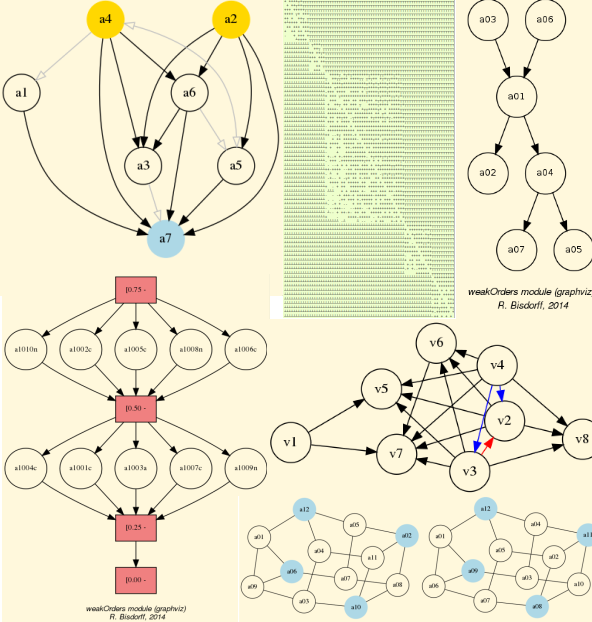
\includegraphics[scale=0.5]{introDoc3.png}
        \end{figure}

        \vspace{10mm}
        \textbf{\Huge {Tutorials and Advanced Topics}}

        \textbf{Raymond BISDORFF}

        \small Luxembourg,  2020

        \small  Last updated : \today
        
        \vspace{10mm}
        \begin{center}
        \emph{This documentation is dedicated to our}\\
        \emph{late colleague and dear friend}\\
         Prof. Marc ROUBENS.
        \end{center}

        %% \vfill adds at the bottom
        \vfill
        \textit{More documents are freely available }{\href{https://digraph3.readthedocs.io/en/latest}{here}}
    \end{titlepage}

    \clearpage
    \pagenumbering{arabic}

    
\pagestyle{plain}

    
    
\pagestyle{normal}
\phantomsection\label{\detokenize{tutorial::doc}}
\begingroup
\sphinxsetup{%
      verbatimwithframe=false,
      VerbatimColor={named}{OldLace},
      %VerbatimHighlightColor={named}{Azure},
      hintBorderColor={named}{LightCoral},
      attentionborder=3pt,
      attentionBorderColor={named}{Crimson},
      attentionBgColor={named}{FloralWhite},
      noteborder=2pt,
      noteBorderColor={named}{Olive},
      cautionborder=3pt,
      cautionBorderColor={named}{Cyan},
      cautionBgColor={named}{LightCyan}}


\phantomsection\label{\detokenize{tutorial:tutorial-label}}

\bigskip\hrule\bigskip


\textbf{\Large{A. Tutorials of the \textsc{Digraph3} Resources}}

\href{https://digraph3.readthedocs.io/en/latest/index.html}{HTML Version}
\vspace{5mm}

\sphinxAtStartPar
The tutorials in this document describe the practical usage of our \sphinxstyleemphasis{Digraph3} Python3 software resources in the field of \sphinxstyleemphasis{Algorithmic Decision Theory} and more specifically in \sphinxstylestrong{outranking} based \sphinxstyleemphasis{Multiple Criteria Decision Aid} (MCDA). They mainly illustrate practical tools for a Master Course  at the University of Luxembourg. The document contains first a set of tutorials introducing the main objects available in the Digraph3 collection of Python3 modules, like \sphinxstylestrong{digraphs}, \sphinxstylestrong{outranking digraphs}, \sphinxstylestrong{performance tableaux} and \sphinxstylestrong{voting profiles}. Some of the tutorials are decision problem oriented and show how to compute the potential \sphinxstylestrong{winner(s)} of an election, how to build a \sphinxstylestrong{best choice recommendation}, or how to \sphinxstylestrong{rate} or \sphinxstylestrong{linearly rank} with multiple incommensurable performance criteria. More graph theoretical tutorials follow. One on working with \sphinxstylestrong{undirected graphs}, followed by tutorials on how to tackle big outranking digraphs. Finally, special tutorials are devoted to \sphinxstyleemphasis{perfect} graphs, like \sphinxstyleemphasis{split}, \sphinxstyleemphasis{interval} and \sphinxstyleemphasis{permutation} graphs, and to \sphinxstyleemphasis{tree\sphinxhyphen{}graphs} and \sphinxstyleemphasis{forests}.

\sphinxtableofcontents


\section{Working with digraphs and outranking digraphs}
\label{\detokenize{tutorial:working-with-digraphs-and-outranking-digraphs}}\label{\detokenize{tutorial:working-with-digraphs-label}}
\sphinxAtStartPar
This first part of the tutorials introduces the Digraph3 software collection of Python programming resources.

\begin{sphinxShadowBox}
\begin{itemize}
\item {} 
\sphinxAtStartPar
\phantomsection\label{\detokenize{tutorial:id243}}{\hyperref[\detokenize{tutorial:working-with-the-digraph3-software-resources}]{\sphinxcrossref{Working with the \sphinxstyleemphasis{Digraph3} software resources}}} (\autopageref*{\detokenize{tutorial:working-with-the-digraph3-software-resources}})

\item {} 
\sphinxAtStartPar
\phantomsection\label{\detokenize{tutorial:id244}}{\hyperref[\detokenize{tutorial:working-with-the-digraphs-module}]{\sphinxcrossref{Working with the \sphinxcode{\sphinxupquote{digraphs}} module}}} (\autopageref*{\detokenize{tutorial:working-with-the-digraphs-module}})

\item {} 
\sphinxAtStartPar
\phantomsection\label{\detokenize{tutorial:id245}}{\hyperref[\detokenize{tutorial:working-with-the-outrankingdigraphs-module}]{\sphinxcrossref{Working with the \sphinxcode{\sphinxupquote{outrankingDigraphs}} module}}} (\autopageref*{\detokenize{tutorial:working-with-the-outrankingdigraphs-module}})

\end{itemize}
\end{sphinxShadowBox}


\bigskip\hrule\bigskip



\subsection{Working with the \sphinxstyleemphasis{Digraph3} software resources}
\label{\detokenize{tutorial:working-with-the-digraph3-software-resources}}\label{\detokenize{tutorial:digraphs-tutorial-label}}
\begin{sphinxShadowBox}
\begin{itemize}
\item {} 
\sphinxAtStartPar
\phantomsection\label{\detokenize{tutorial:id246}}{\hyperref[\detokenize{tutorial:purpose}]{\sphinxcrossref{Purpose}}} (\autopageref*{\detokenize{tutorial:purpose}})

\item {} 
\sphinxAtStartPar
\phantomsection\label{\detokenize{tutorial:id247}}{\hyperref[\detokenize{tutorial:downloading-of-the-digraph3-resources}]{\sphinxcrossref{Downloading of the Digraph3 resources}}} (\autopageref*{\detokenize{tutorial:downloading-of-the-digraph3-resources}})

\item {} 
\sphinxAtStartPar
\phantomsection\label{\detokenize{tutorial:id248}}{\hyperref[\detokenize{tutorial:starting-a-python3-terminal-session}]{\sphinxcrossref{Starting a Python3 terminal session}}} (\autopageref*{\detokenize{tutorial:starting-a-python3-terminal-session}})

\item {} 
\sphinxAtStartPar
\phantomsection\label{\detokenize{tutorial:id249}}{\hyperref[\detokenize{tutorial:digraph-object-structure}]{\sphinxcrossref{\sphinxstyleemphasis{Digraph} object structure}}} (\autopageref*{\detokenize{tutorial:digraph-object-structure}})

\item {} 
\sphinxAtStartPar
\phantomsection\label{\detokenize{tutorial:id250}}{\hyperref[\detokenize{tutorial:permanent-storage}]{\sphinxcrossref{Permanent storage}}} (\autopageref*{\detokenize{tutorial:permanent-storage}})

\item {} 
\sphinxAtStartPar
\phantomsection\label{\detokenize{tutorial:id251}}{\hyperref[\detokenize{tutorial:inspecting-a-digraph-object}]{\sphinxcrossref{Inspecting a \sphinxstyleemphasis{Digraph} object}}} (\autopageref*{\detokenize{tutorial:inspecting-a-digraph-object}})

\item {} 
\sphinxAtStartPar
\phantomsection\label{\detokenize{tutorial:id252}}{\hyperref[\detokenize{tutorial:special-digraph-instances}]{\sphinxcrossref{Special \sphinxstyleemphasis{Digraph} instances}}} (\autopageref*{\detokenize{tutorial:special-digraph-instances}})

\end{itemize}
\end{sphinxShadowBox}


\subsubsection{Purpose}
\label{\detokenize{tutorial:purpose}}
\sphinxAtStartPar
The basic idea of the Digraph3 Python resources is to make easy python interactive sessions or write short Python3 scripts for computing all kind of results from a bipolar\sphinxhyphen{}valued digraph or graph. These include such features as maximal independent, maximal dominant or absorbent choices, rankings, outrankings, linear ordering, etc. Most of the available computing resources are meant to illustrate a Master Course  on \emph{Algorithmic Decision Theory} given at the University of Luxembourg in the context of its \sphinxstyleemphasis{Master in Information and Computer Science} (MICS).

\sphinxAtStartPar
The Python development of these computing resources offers the advantage of an easy to write and maintain OOP source code as expected from a performing scripting language without loosing on efficiency in execution times compared to compiled languages such as C++ or Java.


\subsubsection{Downloading of the Digraph3 resources}
\label{\detokenize{tutorial:downloading-of-the-digraph3-resources}}
\sphinxAtStartPar
Using the Digraph3 modules is easy. You only need to have installed on your system the \sphinxhref{https://www.python.org/doc/}{Python} (https://www.python.org/doc/) programming language of version 3.+ (readily available under Linux and Mac OS).

\sphinxAtStartPar
Several download options (easiest under Linux or Mac OS\sphinxhyphen{}X) are given.
\begin{enumerate}
\sphinxsetlistlabels{\arabic}{enumi}{enumii}{}{.}%
\item {} 
\sphinxAtStartPar
(\sphinxstyleemphasis{Recommended}) With a browser access, download and extract the latest distribution zip archive from

\sphinxAtStartPar
\sphinxurl{https://github.com/rbisdorff/Digraph3}  or, from

\sphinxAtStartPar
\sphinxurl{https://sourceforge.net/projects/digraph3}

\item {} 
\sphinxAtStartPar
By using a git client either, cloning from github

\end{enumerate}

\begin{sphinxVerbatim}[commandchars=\\\{\}]
...\PYGZdl{}\PYG{+w}{ }git\PYG{+w}{ }clone\PYG{+w}{ }https://github.com/rbisdorff/Digraph3
\end{sphinxVerbatim}
\begin{enumerate}
\sphinxsetlistlabels{\arabic}{enumi}{enumii}{}{.}%
\setcounter{enumi}{2}
\item {} 
\sphinxAtStartPar
Or, from sourceforge.net

\end{enumerate}

\begin{sphinxVerbatim}[commandchars=\\\{\}]
...\PYGZdl{}\PYG{+w}{ }git\PYG{+w}{ }clone\PYG{+w}{ }https://git.code.sf.net/p/digraph3/code\PYG{+w}{ }Digraph3
\end{sphinxVerbatim}


\subsubsection{Starting a Python3 terminal session}
\label{\detokenize{tutorial:starting-a-python3-terminal-session}}
\sphinxAtStartPar
You may start an interactive Python3 terminal session in the \sphinxstyleemphasis{Digraph3} directory.

\begin{sphinxVerbatim}[commandchars=\\\{\},numbers=left,firstnumber=1,stepnumber=1]
\PYG{n+nv}{\PYGZdl{}HOME}/.../Digraph3\PYGZdl{}\PYG{+w}{ }python3
Python\PYG{+w}{ }\PYG{l+m}{3}.10.0\PYG{+w}{ }\PYG{o}{(}default,\PYG{+w}{ }Oct\PYG{+w}{ }\PYG{l+m}{21}\PYG{+w}{ }\PYG{l+m}{2021},\PYG{+w}{ }\PYG{l+m}{10}:53:53\PYG{o}{)}
\PYG{o}{[}GCC\PYG{+w}{ }\PYG{l+m}{11}.2.0\PYG{o}{]}\PYG{+w}{ }on\PYG{+w}{ }linux\PYG{+w}{ }Type\PYG{+w}{ }\PYG{l+s+s2}{\PYGZdq{}help\PYGZdq{}},\PYG{+w}{ }\PYG{l+s+s2}{\PYGZdq{}copyright\PYGZdq{}},
\PYG{l+s+s2}{\PYGZdq{}credits\PYGZdq{}}\PYG{+w}{ }or\PYG{+w}{ }\PYG{l+s+s2}{\PYGZdq{}license\PYGZdq{}}\PYG{+w}{ }\PYG{k}{for}\PYG{+w}{ }more\PYG{+w}{ }information.
\PYGZgt{}\PYGZgt{}\PYGZgt{}
\end{sphinxVerbatim}

\sphinxAtStartPar
For exploring the classes and methods provided by the \sphinxstyleemphasis{Digraph3} modules (see the \sphinxhref{techDoc.html}{Reference manual}) enter the \sphinxstyleemphasis{Python3} commands following the session prompts marked with \sphinxcode{\sphinxupquote{\textgreater{}\textgreater{}\textgreater{}}} or \sphinxcode{\sphinxupquote{...}} . The lines without the prompt are console output from the Python3 interpreter.
\sphinxSetupCaptionForVerbatim{Generating a random digraph instance}
\def\sphinxLiteralBlockLabel{\label{\detokenize{tutorial:digraphs}}}
\fvset{hllines={, 3, 11, 12,}}%
\begin{sphinxVerbatim}[commandchars=\\\{\},numbers=left,firstnumber=1,stepnumber=1]
\PYG{g+gp}{\PYGZgt{}\PYGZgt{}\PYGZgt{} }\PYG{k+kn}{from} \PYG{n+nn}{randomDigraphs} \PYG{k+kn}{import} \PYG{n}{RandomDigraph}
\PYG{g+gp}{\PYGZgt{}\PYGZgt{}\PYGZgt{} }\PYG{n}{dg} \PYG{o}{=} \PYG{n}{RandomDigraph}\PYG{p}{(}\PYG{n}{order}\PYG{o}{=}\PYG{l+m+mi}{5}\PYG{p}{,}\PYG{n}{arcProbability}\PYG{o}{=}\PYG{l+m+mf}{0.5}\PYG{p}{,}\PYG{n}{seed}\PYG{o}{=}\PYG{l+m+mi}{101}\PYG{p}{)}
\PYG{g+gp}{\PYGZgt{}\PYGZgt{}\PYGZgt{} }\PYG{n}{dg}
\PYG{g+go}{ *\PYGZhy{}\PYGZhy{}\PYGZhy{}\PYGZhy{}\PYGZhy{}\PYGZhy{}\PYGZhy{} Digraph instance description \PYGZhy{}\PYGZhy{}\PYGZhy{}\PYGZhy{}\PYGZhy{}\PYGZhy{}*}
\PYG{g+go}{ Instance class   : RandomDigraph}
\PYG{g+go}{ Instance name    : randomDigraph}
\PYG{g+go}{ Digraph Order      : 5}
\PYG{g+go}{ Digraph Size       : 12}
\PYG{g+go}{ Valuation domain : [\PYGZhy{}1.00; 1.00]}
\PYG{g+go}{ Determinateness  : 100.000}
\PYG{g+go}{ Attributes       : [\PYGZsq{}actions\PYGZsq{}, \PYGZsq{}valuationdomain\PYGZsq{}, \PYGZsq{}relation\PYGZsq{},}
\PYG{g+go}{                     \PYGZsq{}order\PYGZsq{}, \PYGZsq{}name\PYGZsq{}, \PYGZsq{}gamma\PYGZsq{}, \PYGZsq{}notGamma\PYGZsq{},}
\PYG{g+go}{                     \PYGZsq{}seed\PYGZsq{}, \PYGZsq{}arcProbability\PYGZsq{}, ]}
\end{sphinxVerbatim}
\sphinxresetverbatimhllines

\sphinxAtStartPar
In \hyperref[\detokenize{tutorial:digraphs}]{Listing \ref{\detokenize{tutorial:digraphs}}} we import, for instance, from the \sphinxcode{\sphinxupquote{randomDigraphs}} module the \sphinxcode{\sphinxupquote{RandomDigraph}} class in order to generate a random \sphinxstyleemphasis{digraph} object \sphinxstyleemphasis{dg} of order 5 \sphinxhyphen{} number of nodes called (decision) \sphinxstyleemphasis{actions} \sphinxhyphen{} and arc probability of 50\%. We may directly inspect the content of python object \sphinxstyleemphasis{dg} (Line 3).
\begin{quote}

\begin{sphinxadmonition}{note}{Note:}
\sphinxAtStartPar
For convenience of redoing the computations, all python code\sphinxhyphen{}blocks show in the upper right corner a specific \sphinxstylestrong{copy button} which allows to both copy \sphinxstyleemphasis{only} code lines, i.e. lines starting with ‘\textgreater{}\textgreater{}\textgreater{}’ or ‘…’, and stripping the console prompts. The copied code lines may hence be right away \sphinxstyleemphasis{pasted} into a Python console session.
\end{sphinxadmonition}
\end{quote}


\subsubsection{\sphinxstyleemphasis{Digraph} object structure}
\label{\detokenize{tutorial:digraph-object-structure}}
\sphinxAtStartPar
All \sphinxcode{\sphinxupquote{Digraph}} objects contain at least the following attributes (see \hyperref[\detokenize{tutorial:digraphs}]{Listing \ref{\detokenize{tutorial:digraphs}}} Lines 11\sphinxhyphen{}12):
\begin{enumerate}
\sphinxsetlistlabels{\arabic}{enumi}{enumii}{}{.}%
\setcounter{enumi}{-1}
\item {} 
\sphinxAtStartPar
A \sphinxstylestrong{name} attribute, holding usually the actual name of the stored instance that was used to create the instance;

\item {} 
\sphinxAtStartPar
A ordered dictionary of digraph nodes called \sphinxstylestrong{actions} (decision alternatives) with at least a ‘name’ attribute;

\item {} 
\sphinxAtStartPar
An \sphinxstylestrong{order} attribute containing the number of graph nodes (length of the actions dictionary) automatically added by the object constructor;

\item {} 
\sphinxAtStartPar
A logical characteristic \sphinxstylestrong{valuationdomain} dictionary with three decimal entries: the minimum (\sphinxhyphen{}1.0, means certainly false), the median (0.0, means missing information) and the maximum characteristic value (+1.0, means certainly true);

\item {} 
\sphinxAtStartPar
A double dictionary called \sphinxstylestrong{relation} and indexed by an oriented pair of actions (nodes) and carrying a decimal characteristic value in the range of the previous valuation domain;

\item {} 
\sphinxAtStartPar
Its associated \sphinxstylestrong{gamma} attribute, a dictionary containing the direct successors, respectively predecessors of each action, automatically added by the object constructor;

\item {} 
\sphinxAtStartPar
Its associated \sphinxstylestrong{notGamma} attribute, a dictionary containing the actions that are not direct successors respectively predecessors of each action, automatically added by the object constructor.

\end{enumerate}


\subsubsection{Permanent storage}
\label{\detokenize{tutorial:permanent-storage}}
\sphinxAtStartPar
The \sphinxcode{\sphinxupquote{save()}} method stores the digraph object \sphinxstyleemphasis{dg} in a file named ‘tutorialDigraph.py’,

\begin{sphinxVerbatim}[commandchars=\\\{\}]
\PYG{g+gp}{\PYGZgt{}\PYGZgt{}\PYGZgt{} }\PYG{n}{dg}\PYG{o}{.}\PYG{n}{save}\PYG{p}{(}\PYG{l+s+s1}{\PYGZsq{}}\PYG{l+s+s1}{tutorialDigraph}\PYG{l+s+s1}{\PYGZsq{}}\PYG{p}{)}
\PYG{g+go}{ *\PYGZhy{}\PYGZhy{}\PYGZhy{} Saving digraph in file: \PYGZlt{}tutorialDigraph.py\PYGZgt{} \PYGZhy{}\PYGZhy{}\PYGZhy{}*}
\end{sphinxVerbatim}

\sphinxAtStartPar
with the following content

\begin{sphinxVerbatim}[commandchars=\\\{\},numbers=left,firstnumber=1,stepnumber=1]
\PYG{k+kn}{from} \PYG{n+nn}{decimal} \PYG{k+kn}{import} \PYG{n}{Decimal}
\PYG{k+kn}{from} \PYG{n+nn}{collections} \PYG{k+kn}{import} \PYG{n}{OrderedDict}
\PYG{n}{actions} \PYG{o}{=} \PYG{n}{OrderedDict}\PYG{p}{(}\PYG{p}{[}
 \PYG{p}{(}\PYG{l+s+s1}{\PYGZsq{}}\PYG{l+s+s1}{a1}\PYG{l+s+s1}{\PYGZsq{}}\PYG{p}{,} \PYG{p}{\PYGZob{}}\PYG{l+s+s1}{\PYGZsq{}}\PYG{l+s+s1}{shortName}\PYG{l+s+s1}{\PYGZsq{}}\PYG{p}{:} \PYG{l+s+s1}{\PYGZsq{}}\PYG{l+s+s1}{a1}\PYG{l+s+s1}{\PYGZsq{}}\PYG{p}{,} \PYG{l+s+s1}{\PYGZsq{}}\PYG{l+s+s1}{name}\PYG{l+s+s1}{\PYGZsq{}}\PYG{p}{:} \PYG{l+s+s1}{\PYGZsq{}}\PYG{l+s+s1}{random decision action}\PYG{l+s+s1}{\PYGZsq{}}\PYG{p}{\PYGZcb{}}\PYG{p}{)}\PYG{p}{,}
 \PYG{p}{(}\PYG{l+s+s1}{\PYGZsq{}}\PYG{l+s+s1}{a2}\PYG{l+s+s1}{\PYGZsq{}}\PYG{p}{,} \PYG{p}{\PYGZob{}}\PYG{l+s+s1}{\PYGZsq{}}\PYG{l+s+s1}{shortName}\PYG{l+s+s1}{\PYGZsq{}}\PYG{p}{:} \PYG{l+s+s1}{\PYGZsq{}}\PYG{l+s+s1}{a2}\PYG{l+s+s1}{\PYGZsq{}}\PYG{p}{,} \PYG{l+s+s1}{\PYGZsq{}}\PYG{l+s+s1}{name}\PYG{l+s+s1}{\PYGZsq{}}\PYG{p}{:} \PYG{l+s+s1}{\PYGZsq{}}\PYG{l+s+s1}{random decision action}\PYG{l+s+s1}{\PYGZsq{}}\PYG{p}{\PYGZcb{}}\PYG{p}{)}\PYG{p}{,}
 \PYG{p}{(}\PYG{l+s+s1}{\PYGZsq{}}\PYG{l+s+s1}{a3}\PYG{l+s+s1}{\PYGZsq{}}\PYG{p}{,} \PYG{p}{\PYGZob{}}\PYG{l+s+s1}{\PYGZsq{}}\PYG{l+s+s1}{shortName}\PYG{l+s+s1}{\PYGZsq{}}\PYG{p}{:} \PYG{l+s+s1}{\PYGZsq{}}\PYG{l+s+s1}{a3}\PYG{l+s+s1}{\PYGZsq{}}\PYG{p}{,} \PYG{l+s+s1}{\PYGZsq{}}\PYG{l+s+s1}{name}\PYG{l+s+s1}{\PYGZsq{}}\PYG{p}{:} \PYG{l+s+s1}{\PYGZsq{}}\PYG{l+s+s1}{random decision action}\PYG{l+s+s1}{\PYGZsq{}}\PYG{p}{\PYGZcb{}}\PYG{p}{)}\PYG{p}{,}
 \PYG{p}{(}\PYG{l+s+s1}{\PYGZsq{}}\PYG{l+s+s1}{a4}\PYG{l+s+s1}{\PYGZsq{}}\PYG{p}{,} \PYG{p}{\PYGZob{}}\PYG{l+s+s1}{\PYGZsq{}}\PYG{l+s+s1}{shortName}\PYG{l+s+s1}{\PYGZsq{}}\PYG{p}{:} \PYG{l+s+s1}{\PYGZsq{}}\PYG{l+s+s1}{a4}\PYG{l+s+s1}{\PYGZsq{}}\PYG{p}{,} \PYG{l+s+s1}{\PYGZsq{}}\PYG{l+s+s1}{name}\PYG{l+s+s1}{\PYGZsq{}}\PYG{p}{:} \PYG{l+s+s1}{\PYGZsq{}}\PYG{l+s+s1}{random decision action}\PYG{l+s+s1}{\PYGZsq{}}\PYG{p}{\PYGZcb{}}\PYG{p}{)}\PYG{p}{,}
 \PYG{p}{(}\PYG{l+s+s1}{\PYGZsq{}}\PYG{l+s+s1}{a5}\PYG{l+s+s1}{\PYGZsq{}}\PYG{p}{,} \PYG{p}{\PYGZob{}}\PYG{l+s+s1}{\PYGZsq{}}\PYG{l+s+s1}{shortName}\PYG{l+s+s1}{\PYGZsq{}}\PYG{p}{:} \PYG{l+s+s1}{\PYGZsq{}}\PYG{l+s+s1}{a5}\PYG{l+s+s1}{\PYGZsq{}}\PYG{p}{,} \PYG{l+s+s1}{\PYGZsq{}}\PYG{l+s+s1}{name}\PYG{l+s+s1}{\PYGZsq{}}\PYG{p}{:} \PYG{l+s+s1}{\PYGZsq{}}\PYG{l+s+s1}{random decision action}\PYG{l+s+s1}{\PYGZsq{}}\PYG{p}{\PYGZcb{}}\PYG{p}{)}\PYG{p}{,}
 \PYG{p}{]}\PYG{p}{)}
\PYG{n}{valuationdomain} \PYG{o}{=} \PYG{p}{\PYGZob{}}\PYG{l+s+s1}{\PYGZsq{}}\PYG{l+s+s1}{min}\PYG{l+s+s1}{\PYGZsq{}}\PYG{p}{:} \PYG{n}{Decimal}\PYG{p}{(}\PYG{l+s+s1}{\PYGZsq{}}\PYG{l+s+s1}{\PYGZhy{}1.0}\PYG{l+s+s1}{\PYGZsq{}}\PYG{p}{)}\PYG{p}{,}
                   \PYG{l+s+s1}{\PYGZsq{}}\PYG{l+s+s1}{med}\PYG{l+s+s1}{\PYGZsq{}}\PYG{p}{:} \PYG{n}{Decimal}\PYG{p}{(}\PYG{l+s+s1}{\PYGZsq{}}\PYG{l+s+s1}{0.0}\PYG{l+s+s1}{\PYGZsq{}}\PYG{p}{)}\PYG{p}{,}
                   \PYG{l+s+s1}{\PYGZsq{}}\PYG{l+s+s1}{max}\PYG{l+s+s1}{\PYGZsq{}}\PYG{p}{:} \PYG{n}{Decimal}\PYG{p}{(}\PYG{l+s+s1}{\PYGZsq{}}\PYG{l+s+s1}{1.0}\PYG{l+s+s1}{\PYGZsq{}}\PYG{p}{)}\PYG{p}{,}
                   \PYG{l+s+s1}{\PYGZsq{}}\PYG{l+s+s1}{hasIntegerValuation}\PYG{l+s+s1}{\PYGZsq{}}\PYG{p}{:} \PYG{k+kc}{True}\PYG{p}{,} \PYG{c+c1}{\PYGZsh{} repr. format}
                   \PYG{p}{\PYGZcb{}}
\PYG{n}{relation} \PYG{o}{=} \PYG{p}{\PYGZob{}}
 \PYG{l+s+s1}{\PYGZsq{}}\PYG{l+s+s1}{a1}\PYG{l+s+s1}{\PYGZsq{}}\PYG{p}{:} \PYG{p}{\PYGZob{}}\PYG{l+s+s1}{\PYGZsq{}}\PYG{l+s+s1}{a1}\PYG{l+s+s1}{\PYGZsq{}}\PYG{p}{:}\PYG{n}{Decimal}\PYG{p}{(}\PYG{l+s+s1}{\PYGZsq{}}\PYG{l+s+s1}{\PYGZhy{}1.0}\PYG{l+s+s1}{\PYGZsq{}}\PYG{p}{)}\PYG{p}{,} \PYG{l+s+s1}{\PYGZsq{}}\PYG{l+s+s1}{a2}\PYG{l+s+s1}{\PYGZsq{}}\PYG{p}{:}\PYG{n}{Decimal}\PYG{p}{(}\PYG{l+s+s1}{\PYGZsq{}}\PYG{l+s+s1}{\PYGZhy{}1.0}\PYG{l+s+s1}{\PYGZsq{}}\PYG{p}{)}\PYG{p}{,}
        \PYG{l+s+s1}{\PYGZsq{}}\PYG{l+s+s1}{a3}\PYG{l+s+s1}{\PYGZsq{}}\PYG{p}{:}\PYG{n}{Decimal}\PYG{p}{(}\PYG{l+s+s1}{\PYGZsq{}}\PYG{l+s+s1}{1.0}\PYG{l+s+s1}{\PYGZsq{}}\PYG{p}{)}\PYG{p}{,} \PYG{l+s+s1}{\PYGZsq{}}\PYG{l+s+s1}{a4}\PYG{l+s+s1}{\PYGZsq{}}\PYG{p}{:}\PYG{n}{Decimal}\PYG{p}{(}\PYG{l+s+s1}{\PYGZsq{}}\PYG{l+s+s1}{\PYGZhy{}1.0}\PYG{l+s+s1}{\PYGZsq{}}\PYG{p}{)}\PYG{p}{,}
        \PYG{l+s+s1}{\PYGZsq{}}\PYG{l+s+s1}{a5}\PYG{l+s+s1}{\PYGZsq{}}\PYG{p}{:}\PYG{n}{Decimal}\PYG{p}{(}\PYG{l+s+s1}{\PYGZsq{}}\PYG{l+s+s1}{\PYGZhy{}1.0}\PYG{l+s+s1}{\PYGZsq{}}\PYG{p}{)}\PYG{p}{,}\PYG{p}{\PYGZcb{}}\PYG{p}{,}
 \PYG{l+s+s1}{\PYGZsq{}}\PYG{l+s+s1}{a2}\PYG{l+s+s1}{\PYGZsq{}}\PYG{p}{:} \PYG{p}{\PYGZob{}}\PYG{l+s+s1}{\PYGZsq{}}\PYG{l+s+s1}{a1}\PYG{l+s+s1}{\PYGZsq{}}\PYG{p}{:}\PYG{n}{Decimal}\PYG{p}{(}\PYG{l+s+s1}{\PYGZsq{}}\PYG{l+s+s1}{1.0}\PYG{l+s+s1}{\PYGZsq{}}\PYG{p}{)}\PYG{p}{,} \PYG{l+s+s1}{\PYGZsq{}}\PYG{l+s+s1}{a2}\PYG{l+s+s1}{\PYGZsq{}}\PYG{p}{:}\PYG{n}{Decimal}\PYG{p}{(}\PYG{l+s+s1}{\PYGZsq{}}\PYG{l+s+s1}{\PYGZhy{}1.0}\PYG{l+s+s1}{\PYGZsq{}}\PYG{p}{)}\PYG{p}{,}
        \PYG{l+s+s1}{\PYGZsq{}}\PYG{l+s+s1}{a3}\PYG{l+s+s1}{\PYGZsq{}}\PYG{p}{:}\PYG{n}{Decimal}\PYG{p}{(}\PYG{l+s+s1}{\PYGZsq{}}\PYG{l+s+s1}{\PYGZhy{}1.0}\PYG{l+s+s1}{\PYGZsq{}}\PYG{p}{)}\PYG{p}{,} \PYG{l+s+s1}{\PYGZsq{}}\PYG{l+s+s1}{a4}\PYG{l+s+s1}{\PYGZsq{}}\PYG{p}{:}\PYG{n}{Decimal}\PYG{p}{(}\PYG{l+s+s1}{\PYGZsq{}}\PYG{l+s+s1}{1.0}\PYG{l+s+s1}{\PYGZsq{}}\PYG{p}{)}\PYG{p}{,}
        \PYG{l+s+s1}{\PYGZsq{}}\PYG{l+s+s1}{a5}\PYG{l+s+s1}{\PYGZsq{}}\PYG{p}{:}\PYG{n}{Decimal}\PYG{p}{(}\PYG{l+s+s1}{\PYGZsq{}}\PYG{l+s+s1}{1.0}\PYG{l+s+s1}{\PYGZsq{}}\PYG{p}{)}\PYG{p}{,}\PYG{p}{\PYGZcb{}}\PYG{p}{,}
 \PYG{l+s+s1}{\PYGZsq{}}\PYG{l+s+s1}{a3}\PYG{l+s+s1}{\PYGZsq{}}\PYG{p}{:} \PYG{p}{\PYGZob{}}\PYG{l+s+s1}{\PYGZsq{}}\PYG{l+s+s1}{a1}\PYG{l+s+s1}{\PYGZsq{}}\PYG{p}{:}\PYG{n}{Decimal}\PYG{p}{(}\PYG{l+s+s1}{\PYGZsq{}}\PYG{l+s+s1}{1.0}\PYG{l+s+s1}{\PYGZsq{}}\PYG{p}{)}\PYG{p}{,} \PYG{l+s+s1}{\PYGZsq{}}\PYG{l+s+s1}{a2}\PYG{l+s+s1}{\PYGZsq{}}\PYG{p}{:}\PYG{n}{Decimal}\PYG{p}{(}\PYG{l+s+s1}{\PYGZsq{}}\PYG{l+s+s1}{\PYGZhy{}1.0}\PYG{l+s+s1}{\PYGZsq{}}\PYG{p}{)}\PYG{p}{,}
        \PYG{l+s+s1}{\PYGZsq{}}\PYG{l+s+s1}{a3}\PYG{l+s+s1}{\PYGZsq{}}\PYG{p}{:}\PYG{n}{Decimal}\PYG{p}{(}\PYG{l+s+s1}{\PYGZsq{}}\PYG{l+s+s1}{\PYGZhy{}1.0}\PYG{l+s+s1}{\PYGZsq{}}\PYG{p}{)}\PYG{p}{,} \PYG{l+s+s1}{\PYGZsq{}}\PYG{l+s+s1}{a4}\PYG{l+s+s1}{\PYGZsq{}}\PYG{p}{:}\PYG{n}{Decimal}\PYG{p}{(}\PYG{l+s+s1}{\PYGZsq{}}\PYG{l+s+s1}{1.0}\PYG{l+s+s1}{\PYGZsq{}}\PYG{p}{)}\PYG{p}{,}
        \PYG{l+s+s1}{\PYGZsq{}}\PYG{l+s+s1}{a5}\PYG{l+s+s1}{\PYGZsq{}}\PYG{p}{:}\PYG{n}{Decimal}\PYG{p}{(}\PYG{l+s+s1}{\PYGZsq{}}\PYG{l+s+s1}{\PYGZhy{}1.0}\PYG{l+s+s1}{\PYGZsq{}}\PYG{p}{)}\PYG{p}{,}\PYG{p}{\PYGZcb{}}\PYG{p}{,}
 \PYG{l+s+s1}{\PYGZsq{}}\PYG{l+s+s1}{a4}\PYG{l+s+s1}{\PYGZsq{}}\PYG{p}{:} \PYG{p}{\PYGZob{}}\PYG{l+s+s1}{\PYGZsq{}}\PYG{l+s+s1}{a1}\PYG{l+s+s1}{\PYGZsq{}}\PYG{p}{:}\PYG{n}{Decimal}\PYG{p}{(}\PYG{l+s+s1}{\PYGZsq{}}\PYG{l+s+s1}{1.0}\PYG{l+s+s1}{\PYGZsq{}}\PYG{p}{)}\PYG{p}{,} \PYG{l+s+s1}{\PYGZsq{}}\PYG{l+s+s1}{a2}\PYG{l+s+s1}{\PYGZsq{}}\PYG{p}{:}\PYG{n}{Decimal}\PYG{p}{(}\PYG{l+s+s1}{\PYGZsq{}}\PYG{l+s+s1}{1.0}\PYG{l+s+s1}{\PYGZsq{}}\PYG{p}{)}\PYG{p}{,}
        \PYG{l+s+s1}{\PYGZsq{}}\PYG{l+s+s1}{a3}\PYG{l+s+s1}{\PYGZsq{}}\PYG{p}{:}\PYG{n}{Decimal}\PYG{p}{(}\PYG{l+s+s1}{\PYGZsq{}}\PYG{l+s+s1}{1.0}\PYG{l+s+s1}{\PYGZsq{}}\PYG{p}{)}\PYG{p}{,} \PYG{l+s+s1}{\PYGZsq{}}\PYG{l+s+s1}{a4}\PYG{l+s+s1}{\PYGZsq{}}\PYG{p}{:}\PYG{n}{Decimal}\PYG{p}{(}\PYG{l+s+s1}{\PYGZsq{}}\PYG{l+s+s1}{\PYGZhy{}1.0}\PYG{l+s+s1}{\PYGZsq{}}\PYG{p}{)}\PYG{p}{,}
        \PYG{l+s+s1}{\PYGZsq{}}\PYG{l+s+s1}{a5}\PYG{l+s+s1}{\PYGZsq{}}\PYG{p}{:}\PYG{n}{Decimal}\PYG{p}{(}\PYG{l+s+s1}{\PYGZsq{}}\PYG{l+s+s1}{\PYGZhy{}1.0}\PYG{l+s+s1}{\PYGZsq{}}\PYG{p}{)}\PYG{p}{,}\PYG{p}{\PYGZcb{}}\PYG{p}{,}
 \PYG{l+s+s1}{\PYGZsq{}}\PYG{l+s+s1}{a5}\PYG{l+s+s1}{\PYGZsq{}}\PYG{p}{:} \PYG{p}{\PYGZob{}}\PYG{l+s+s1}{\PYGZsq{}}\PYG{l+s+s1}{a1}\PYG{l+s+s1}{\PYGZsq{}}\PYG{p}{:}\PYG{n}{Decimal}\PYG{p}{(}\PYG{l+s+s1}{\PYGZsq{}}\PYG{l+s+s1}{1.0}\PYG{l+s+s1}{\PYGZsq{}}\PYG{p}{)}\PYG{p}{,} \PYG{l+s+s1}{\PYGZsq{}}\PYG{l+s+s1}{a2}\PYG{l+s+s1}{\PYGZsq{}}\PYG{p}{:}\PYG{n}{Decimal}\PYG{p}{(}\PYG{l+s+s1}{\PYGZsq{}}\PYG{l+s+s1}{1.0}\PYG{l+s+s1}{\PYGZsq{}}\PYG{p}{)}\PYG{p}{,}
        \PYG{l+s+s1}{\PYGZsq{}}\PYG{l+s+s1}{a3}\PYG{l+s+s1}{\PYGZsq{}}\PYG{p}{:}\PYG{n}{Decimal}\PYG{p}{(}\PYG{l+s+s1}{\PYGZsq{}}\PYG{l+s+s1}{1.0}\PYG{l+s+s1}{\PYGZsq{}}\PYG{p}{)}\PYG{p}{,} \PYG{l+s+s1}{\PYGZsq{}}\PYG{l+s+s1}{a4}\PYG{l+s+s1}{\PYGZsq{}}\PYG{p}{:}\PYG{n}{Decimal}\PYG{p}{(}\PYG{l+s+s1}{\PYGZsq{}}\PYG{l+s+s1}{\PYGZhy{}1.0}\PYG{l+s+s1}{\PYGZsq{}}\PYG{p}{)}\PYG{p}{,}
        \PYG{l+s+s1}{\PYGZsq{}}\PYG{l+s+s1}{a5}\PYG{l+s+s1}{\PYGZsq{}}\PYG{p}{:}\PYG{n}{Decimal}\PYG{p}{(}\PYG{l+s+s1}{\PYGZsq{}}\PYG{l+s+s1}{\PYGZhy{}1.0}\PYG{l+s+s1}{\PYGZsq{}}\PYG{p}{)}\PYG{p}{,}\PYG{p}{\PYGZcb{}}\PYG{p}{,}
 \PYG{p}{\PYGZcb{}}
\end{sphinxVerbatim}


\subsubsection{Inspecting a \sphinxstyleemphasis{Digraph} object}
\label{\detokenize{tutorial:inspecting-a-digraph-object}}
\sphinxAtStartPar
We may reload (see \hyperref[\detokenize{tutorial:tutorialdigraph}]{Listing \ref{\detokenize{tutorial:tutorialdigraph}}}) the previously saved digraph object from the file named ‘tutorialDigraph.py’ with the \sphinxcode{\sphinxupquote{Digraph}} class constructor and different \sphinxstyleemphasis{show} methods (see \hyperref[\detokenize{tutorial:tutorialdigraph}]{Listing \ref{\detokenize{tutorial:tutorialdigraph}}} below) reveal us that \sphinxstyleemphasis{dg} is a \sphinxstyleemphasis{crisp}, \sphinxstyleemphasis{irreflexive}  and \sphinxstyleemphasis{connected} digraph of \sphinxstyleemphasis{order} five.
\sphinxSetupCaptionForVerbatim{Random crisp digraph example}
\def\sphinxLiteralBlockLabel{\label{\detokenize{tutorial:tutorialdigraph}}}
\fvset{hllines={, 3, 18, 28, 31,}}%
\begin{sphinxVerbatim}[commandchars=\\\{\},numbers=left,firstnumber=1,stepnumber=1]
\PYG{g+gp}{\PYGZgt{}\PYGZgt{}\PYGZgt{} }\PYG{k+kn}{from} \PYG{n+nn}{digraphs} \PYG{k+kn}{import} \PYG{n}{Digraph}
\PYG{g+gp}{\PYGZgt{}\PYGZgt{}\PYGZgt{} }\PYG{n}{dg} \PYG{o}{=} \PYG{n}{Digraph}\PYG{p}{(}\PYG{l+s+s1}{\PYGZsq{}}\PYG{l+s+s1}{tutorialDigraph}\PYG{l+s+s1}{\PYGZsq{}}\PYG{p}{)}
\PYG{g+gp}{\PYGZgt{}\PYGZgt{}\PYGZgt{} }\PYG{n}{dg}\PYG{o}{.}\PYG{n}{showShort}\PYG{p}{(}\PYG{p}{)}
\PYG{g+go}{ *\PYGZhy{}\PYGZhy{}\PYGZhy{}\PYGZhy{}\PYGZhy{} show short \PYGZhy{}\PYGZhy{}\PYGZhy{}\PYGZhy{}\PYGZhy{}\PYGZhy{}\PYGZhy{}\PYGZhy{}\PYGZhy{}\PYGZhy{}\PYGZhy{}\PYGZhy{}\PYGZhy{}*}
\PYG{g+go}{ Digraph          : tutorialDigraph}
\PYG{g+go}{ Actions          : OrderedDict([}
\PYG{g+go}{  (\PYGZsq{}a1\PYGZsq{}, \PYGZob{}\PYGZsq{}shortName\PYGZsq{}: \PYGZsq{}a1\PYGZsq{}, \PYGZsq{}name\PYGZsq{}: \PYGZsq{}random decision action\PYGZsq{}\PYGZcb{}),}
\PYG{g+go}{  (\PYGZsq{}a2\PYGZsq{}, \PYGZob{}\PYGZsq{}shortName\PYGZsq{}: \PYGZsq{}a2\PYGZsq{}, \PYGZsq{}name\PYGZsq{}: \PYGZsq{}random decision action\PYGZsq{}\PYGZcb{}),}
\PYG{g+go}{  (\PYGZsq{}a3\PYGZsq{}, \PYGZob{}\PYGZsq{}shortName\PYGZsq{}: \PYGZsq{}a3\PYGZsq{}, \PYGZsq{}name\PYGZsq{}: \PYGZsq{}random decision action\PYGZsq{}\PYGZcb{}),}
\PYG{g+go}{  (\PYGZsq{}a4\PYGZsq{}, \PYGZob{}\PYGZsq{}shortName\PYGZsq{}: \PYGZsq{}a4\PYGZsq{}, \PYGZsq{}name\PYGZsq{}: \PYGZsq{}random decision action\PYGZsq{}\PYGZcb{}),}
\PYG{g+go}{  (\PYGZsq{}a5\PYGZsq{}, \PYGZob{}\PYGZsq{}shortName\PYGZsq{}: \PYGZsq{}a5\PYGZsq{}, \PYGZsq{}name\PYGZsq{}: \PYGZsq{}random decision action\PYGZsq{}\PYGZcb{})}
\PYG{g+go}{  ])}
\PYG{g+go}{ Valuation domain : \PYGZob{}}
\PYG{g+go}{  \PYGZsq{}min\PYGZsq{}: Decimal(\PYGZsq{}\PYGZhy{}1.0\PYGZsq{}),}
\PYG{g+go}{  \PYGZsq{}max\PYGZsq{}: Decimal(\PYGZsq{}1.0\PYGZsq{}),}
\PYG{g+go}{  \PYGZsq{}med\PYGZsq{}: Decimal(\PYGZsq{}0.0\PYGZsq{}), \PYGZsq{}hasIntegerValuation\PYGZsq{}: True}
\PYG{g+go}{  \PYGZcb{}}
\PYG{g+gp}{\PYGZgt{}\PYGZgt{}\PYGZgt{} }\PYG{n}{dg}\PYG{o}{.}\PYG{n}{showRelationTable}\PYG{p}{(}\PYG{p}{)}
\PYG{g+go}{ * \PYGZhy{}\PYGZhy{}\PYGZhy{}\PYGZhy{} Relation Table \PYGZhy{}\PYGZhy{}\PYGZhy{}\PYGZhy{}\PYGZhy{}}
\PYG{g+go}{   S   |  \PYGZsq{}a1\PYGZsq{}  \PYGZsq{}a2\PYGZsq{}  \PYGZsq{}a3\PYGZsq{}  \PYGZsq{}a4\PYGZsq{}  \PYGZsq{}a5\PYGZsq{}}
\PYG{g+go}{ \PYGZhy{}\PYGZhy{}\PYGZhy{}\PYGZhy{}\PYGZhy{}\PYGZhy{}|\PYGZhy{}\PYGZhy{}\PYGZhy{}\PYGZhy{}\PYGZhy{}\PYGZhy{}\PYGZhy{}\PYGZhy{}\PYGZhy{}\PYGZhy{}\PYGZhy{}\PYGZhy{}\PYGZhy{}\PYGZhy{}\PYGZhy{}\PYGZhy{}\PYGZhy{}\PYGZhy{}\PYGZhy{}\PYGZhy{}\PYGZhy{}\PYGZhy{}\PYGZhy{}\PYGZhy{}\PYGZhy{}\PYGZhy{}\PYGZhy{}\PYGZhy{}\PYGZhy{}\PYGZhy{}\PYGZhy{}}
\PYG{g+go}{  \PYGZsq{}a1\PYGZsq{} |   \PYGZhy{}1    \PYGZhy{}1     1    \PYGZhy{}1    \PYGZhy{}1}
\PYG{g+go}{  \PYGZsq{}a2\PYGZsq{} |    1    \PYGZhy{}1    \PYGZhy{}1     1     1}
\PYG{g+go}{  \PYGZsq{}a3\PYGZsq{} |    1    \PYGZhy{}1    \PYGZhy{}1     1    \PYGZhy{}1}
\PYG{g+go}{  \PYGZsq{}a4\PYGZsq{} |    1     1     1    \PYGZhy{}1    \PYGZhy{}1}
\PYG{g+go}{  \PYGZsq{}a5\PYGZsq{} |    1     1     1    \PYGZhy{}1    \PYGZhy{}1}
\PYG{g+go}{ Valuation domain: [\PYGZhy{}1;+1]}
\PYG{g+gp}{\PYGZgt{}\PYGZgt{}\PYGZgt{} }\PYG{n}{dg}\PYG{o}{.}\PYG{n}{showComponents}\PYG{p}{(}\PYG{p}{)}
\PYG{g+go}{ *\PYGZhy{}\PYGZhy{}\PYGZhy{} Connected Components \PYGZhy{}\PYGZhy{}\PYGZhy{}*}
\PYG{g+go}{ 1: [\PYGZsq{}a1\PYGZsq{}, \PYGZsq{}a2\PYGZsq{}, \PYGZsq{}a3\PYGZsq{}, \PYGZsq{}a4\PYGZsq{}, \PYGZsq{}a5\PYGZsq{}]}
\PYG{g+gp}{\PYGZgt{}\PYGZgt{}\PYGZgt{} }\PYG{n}{dg}\PYG{o}{.}\PYG{n}{showNeighborhoods}\PYG{p}{(}\PYG{p}{)}
\PYG{g+go}{ Neighborhoods:}
\PYG{g+go}{   Gamma     :}
\PYG{g+go}{ \PYGZsq{}a1\PYGZsq{}: in =\PYGZgt{} \PYGZob{}\PYGZsq{}a2\PYGZsq{}, \PYGZsq{}a4\PYGZsq{}, \PYGZsq{}a3\PYGZsq{}, \PYGZsq{}a5\PYGZsq{}\PYGZcb{}, out =\PYGZgt{} \PYGZob{}\PYGZsq{}a3\PYGZsq{}\PYGZcb{}}
\PYG{g+go}{ \PYGZsq{}a2\PYGZsq{}: in =\PYGZgt{} \PYGZob{}\PYGZsq{}a5\PYGZsq{}, \PYGZsq{}a4\PYGZsq{}\PYGZcb{}, out =\PYGZgt{} \PYGZob{}\PYGZsq{}a1\PYGZsq{}, \PYGZsq{}a4\PYGZsq{}, \PYGZsq{}a5\PYGZsq{}\PYGZcb{}}
\PYG{g+go}{ \PYGZsq{}a3\PYGZsq{}: in =\PYGZgt{} \PYGZob{}\PYGZsq{}a1\PYGZsq{}, \PYGZsq{}a4\PYGZsq{}, \PYGZsq{}a5\PYGZsq{}\PYGZcb{}, out =\PYGZgt{} \PYGZob{}\PYGZsq{}a1\PYGZsq{}, \PYGZsq{}a4\PYGZsq{}\PYGZcb{}}
\PYG{g+go}{ \PYGZsq{}a4\PYGZsq{}: in =\PYGZgt{} \PYGZob{}\PYGZsq{}a2\PYGZsq{}, \PYGZsq{}a3\PYGZsq{}\PYGZcb{}, out =\PYGZgt{} \PYGZob{}\PYGZsq{}a1\PYGZsq{}, \PYGZsq{}a3\PYGZsq{}, \PYGZsq{}a2\PYGZsq{}\PYGZcb{}}
\PYG{g+go}{ \PYGZsq{}a5\PYGZsq{}: in =\PYGZgt{} \PYGZob{}\PYGZsq{}a2\PYGZsq{}\PYGZcb{}, out =\PYGZgt{} \PYGZob{}\PYGZsq{}a1\PYGZsq{}, \PYGZsq{}a3\PYGZsq{}, \PYGZsq{}a2\PYGZsq{}\PYGZcb{}}
\PYG{g+go}{   Not Gamma :}
\PYG{g+go}{ \PYGZsq{}a1\PYGZsq{}: in =\PYGZgt{} set(), out =\PYGZgt{} \PYGZob{}\PYGZsq{}a2\PYGZsq{}, \PYGZsq{}a4\PYGZsq{}, \PYGZsq{}a5\PYGZsq{}\PYGZcb{}}
\PYG{g+go}{ \PYGZsq{}a2\PYGZsq{}: in =\PYGZgt{} \PYGZob{}\PYGZsq{}a1\PYGZsq{}, \PYGZsq{}a3\PYGZsq{}\PYGZcb{}, out =\PYGZgt{} \PYGZob{}\PYGZsq{}a3\PYGZsq{}\PYGZcb{}}
\PYG{g+go}{ \PYGZsq{}a3\PYGZsq{}: in =\PYGZgt{} \PYGZob{}\PYGZsq{}a2\PYGZsq{}\PYGZcb{}, out =\PYGZgt{} \PYGZob{}\PYGZsq{}a2\PYGZsq{}, \PYGZsq{}a5\PYGZsq{}\PYGZcb{}}
\PYG{g+go}{ \PYGZsq{}a4\PYGZsq{}: in =\PYGZgt{} \PYGZob{}\PYGZsq{}a1\PYGZsq{}, \PYGZsq{}a5\PYGZsq{}\PYGZcb{}, out =\PYGZgt{} \PYGZob{}\PYGZsq{}a5\PYGZsq{}\PYGZcb{}}
\PYG{g+go}{ \PYGZsq{}a5\PYGZsq{}: in =\PYGZgt{} \PYGZob{}\PYGZsq{}a1\PYGZsq{}, \PYGZsq{}a4\PYGZsq{}, \PYGZsq{}a3\PYGZsq{}\PYGZcb{}, out =\PYGZgt{} \PYGZob{}\PYGZsq{}a4\PYGZsq{}\PYGZcb{}}
\end{sphinxVerbatim}
\sphinxresetverbatimhllines

\sphinxAtStartPar
The \sphinxcode{\sphinxupquote{exportGraphViz()}} method generates in
the current working directory a ‘tutorialDigraph.dot’ file and a
‘tutorialdigraph.png’ picture of the tutorial digraph \sphinxstyleemphasis{dg} (see \hyperref[\detokenize{tutorial:tutorialdigraphfig}]{Fig.\@ \ref{\detokenize{tutorial:tutorialdigraphfig}}}), if the \sphinxhref{https://graphviz.org/}{graphviz} (https://graphviz.org/) tools are installed on your system %
\begin{footnote}[1]\sphinxAtStartFootnote
The \sphinxstyleemphasis{exportGraphViz} method is depending on drawing tools from \sphinxhref{https://graphviz.org/}{graphviz} (https://graphviz.org/). On Linux Ubuntu or Debian you may try ‘sudo apt\sphinxhyphen{}get install graphviz’ to install them. There are ready \sphinxstyleemphasis{dmg} installers for Mac OSX.
%
\end{footnote}.

\begin{sphinxVerbatim}[commandchars=\\\{\},numbers=left,firstnumber=1,stepnumber=1]
\PYG{g+gp}{\PYGZgt{}\PYGZgt{}\PYGZgt{} }\PYG{n}{dg}\PYG{o}{.}\PYG{n}{exportGraphViz}\PYG{p}{(}\PYG{l+s+s1}{\PYGZsq{}}\PYG{l+s+s1}{tutorialDigraph}\PYG{l+s+s1}{\PYGZsq{}}\PYG{p}{)}
\PYG{g+go}{ *\PYGZhy{}\PYGZhy{}\PYGZhy{}\PYGZhy{} exporting a dot file do GraphViz tools \PYGZhy{}\PYGZhy{}\PYGZhy{}\PYGZhy{}\PYGZhy{}\PYGZhy{}\PYGZhy{}\PYGZhy{}\PYGZhy{}*}
\PYG{g+go}{ Exporting to tutorialDigraph.dot}
\PYG{g+go}{ dot \PYGZhy{}Grankdir=BT \PYGZhy{}Tpng tutorialDigraph.dot \PYGZhy{}o tutorialDigraph.png}
\end{sphinxVerbatim}

\begin{figure}[H]
\centering
\capstart

\noindent\sphinxincludegraphics[width=300\sphinxpxdimen]{{tutorialDigraph}.png}
\caption{The tutorial crisp digraph}\label{\detokenize{tutorial:tutorialdigraphfig}}\end{figure}

\sphinxAtStartPar
Further methods are provided for inspecting this \sphinxcode{\sphinxupquote{Digraph}} object \sphinxstyleemphasis{dg} , like the following \sphinxcode{\sphinxupquote{showStatistics()}} method.
\sphinxSetupCaptionForVerbatim{Inspecting a Digraph object}
\def\sphinxLiteralBlockLabel{\label{\detokenize{tutorial:showstatistics}}}
\fvset{hllines={, 5, 7, 16,}}%
\begin{sphinxVerbatim}[commandchars=\\\{\},numbers=left,firstnumber=1,stepnumber=1]
\PYG{g+gp}{\PYGZgt{}\PYGZgt{}\PYGZgt{} }\PYG{n}{dg}\PYG{o}{.}\PYG{n}{showStatistics}\PYG{p}{(}\PYG{p}{)}
\PYG{g+go}{ *\PYGZhy{}\PYGZhy{}\PYGZhy{}\PYGZhy{}\PYGZhy{} general statistics \PYGZhy{}\PYGZhy{}\PYGZhy{}\PYGZhy{}\PYGZhy{}\PYGZhy{}\PYGZhy{}\PYGZhy{}\PYGZhy{}\PYGZhy{}\PYGZhy{}\PYGZhy{}\PYGZhy{}*}
\PYG{g+go}{ for digraph              : \PYGZlt{}tutorialDigraph.py\PYGZgt{}}
\PYG{g+go}{ order                    : 5 nodes}
\PYG{g+go}{ size                     : 12 arcs}
\PYG{g+go}{ \PYGZsh{} undetermined           : 0 arcs}
\PYG{g+go}{ determinateness (\PYGZpc{})      : 100.0}
\PYG{g+go}{ arc density              : 0.60}
\PYG{g+go}{ double arc density       : 0.40}
\PYG{g+go}{ single arc density       : 0.40}
\PYG{g+go}{ absence density          : 0.20}
\PYG{g+go}{ strict single arc density: 0.40}
\PYG{g+go}{ strict absence density   : 0.20}
\PYG{g+go}{ \PYGZsh{} components             : 1}
\PYG{g+go}{ \PYGZsh{} strong components      : 1}
\PYG{g+go}{ transitivity degree (\PYGZpc{})  : 60.0}
\PYG{g+go}{                          : [0, 1, 2, 3, 4, 5]}
\PYG{g+go}{ outdegrees distribution  : [0, 1, 1, 3, 0, 0]}
\PYG{g+go}{ indegrees distribution   : [0, 1, 2, 1, 1, 0]}
\PYG{g+go}{ mean outdegree           : 2.40}
\PYG{g+go}{ mean indegree            : 2.40}
\PYG{g+go}{                          : [0, 1, 2, 3, 4, 5, 6, 7, 8, 9, 10]}
\PYG{g+go}{ symmetric degrees dist.  : [0, 0, 0, 0, 1, 4, 0, 0, 0, 0, 0]}
\PYG{g+go}{ mean symmetric degree    : 4.80}
\PYG{g+go}{ outdegrees concentration index   : 0.1667}
\PYG{g+go}{ indegrees concentration index    : 0.2333}
\PYG{g+go}{ symdegrees concentration index   : 0.0333}
\PYG{g+go}{                                  : [0, 1, 2, 3, 4, \PYGZsq{}inf\PYGZsq{}]}
\PYG{g+go}{ neighbourhood depths distribution: [0, 1, 4, 0, 0, 0]}
\PYG{g+go}{ mean neighbourhood depth         : 1.80}
\PYG{g+go}{ digraph diameter                 : 2}
\PYG{g+go}{ agglomeration distribution       :}
\PYG{g+go}{ a1 : 58.33}
\PYG{g+go}{ a2 : 33.33}
\PYG{g+go}{ a3 : 33.33}
\PYG{g+go}{ a4 : 50.00}
\PYG{g+go}{ a5 : 50.00}
\PYG{g+go}{ agglomeration coefficient        : 45.00}
\end{sphinxVerbatim}
\sphinxresetverbatimhllines

\sphinxAtStartPar
These \sphinxstyleemphasis{show} methods usually rely upon corresponding \sphinxstyleemphasis{compute} methods, like the \sphinxcode{\sphinxupquote{computeSize()}}, the \sphinxcode{\sphinxupquote{computeDeterminateness()}} or the \sphinxcode{\sphinxupquote{computeTransitivityDegree()}} method (see \hyperref[\detokenize{tutorial:showstatistics}]{Listing \ref{\detokenize{tutorial:showstatistics}}} Line 5,7,16).

\begin{sphinxVerbatim}[commandchars=\\\{\},numbers=left,firstnumber=1,stepnumber=1]
\PYG{g+gp}{\PYGZgt{}\PYGZgt{}\PYGZgt{} }\PYG{n}{dg}\PYG{o}{.}\PYG{n}{computeSize}\PYG{p}{(}\PYG{p}{)}
\PYG{g+go}{ 12}
\PYG{g+gp}{\PYGZgt{}\PYGZgt{}\PYGZgt{} }\PYG{n}{dg}\PYG{o}{.}\PYG{n}{computeDeterminateness}\PYG{p}{(}\PYG{n}{InPercents}\PYG{o}{=}\PYG{k+kc}{True}\PYG{p}{)}
\PYG{g+go}{ Decimal(\PYGZsq{}100.00\PYGZsq{})}
\PYG{g+gp}{\PYGZgt{}\PYGZgt{}\PYGZgt{} }\PYG{n}{dg}\PYG{o}{.}\PYG{n}{computeTransitivityDegree}\PYG{p}{(}\PYG{n}{InPercents}\PYG{o}{=}\PYG{k+kc}{True}\PYG{p}{)}
\PYG{g+go}{ Decimal(\PYGZsq{}60.00\PYGZsq{})}
\end{sphinxVerbatim}

\sphinxAtStartPar
Mind that \sphinxstyleemphasis{show} methods output their results in the Python console. We provide also some \sphinxstyleemphasis{showHTML} methods which output their results in a system browser’s window.

\begin{sphinxVerbatim}[commandchars=\\\{\}]
\PYG{g+gp}{\PYGZgt{}\PYGZgt{}\PYGZgt{} }\PYG{n}{dg}\PYG{o}{.}\PYG{n}{showHTMLRelationMap}\PYG{p}{(}\PYG{n}{relationName}\PYG{o}{=}\PYG{l+s+s1}{\PYGZsq{}}\PYG{l+s+s1}{r(x,y)}\PYG{l+s+s1}{\PYGZsq{}}\PYG{p}{,}\PYG{n}{rankingRule}\PYG{o}{=}\PYG{k+kc}{None}\PYG{p}{)}
\end{sphinxVerbatim}

\begin{figure}[H]
\centering
\capstart

\noindent\sphinxincludegraphics[width=350\sphinxpxdimen]{{relationMap1}.png}
\caption{Browsing the relation map of the tutorial digraph}\label{\detokenize{tutorial:relationmap1}}\end{figure}

\sphinxAtStartPar
In \hyperref[\detokenize{tutorial:relationmap1}]{Fig.\@ \ref{\detokenize{tutorial:relationmap1}}} we find confirmed again that our random digraph instance \sphinxstyleemphasis{dg}, is indeed a crisp, i.e. 100\% determined digraph instance.


\subsubsection{Special \sphinxstyleemphasis{Digraph} instances}
\label{\detokenize{tutorial:special-digraph-instances}}
\sphinxAtStartPar
Some constructors for universal digraph instances, like the \sphinxcode{\sphinxupquote{CompleteDigraph}}, the \sphinxcode{\sphinxupquote{EmptyDigraph}} or the \sphinxstyleemphasis{circular oriented} \sphinxcode{\sphinxupquote{GridDigraph}} constructor, are readily available (see \hyperref[\detokenize{tutorial:tutorialgrid}]{Fig.\@ \ref{\detokenize{tutorial:tutorialgrid}}}).

\fvset{hllines={, 2,}}%
\begin{sphinxVerbatim}[commandchars=\\\{\},numbers=left,firstnumber=1,stepnumber=1]
\PYG{g+gp}{\PYGZgt{}\PYGZgt{}\PYGZgt{} }\PYG{k+kn}{from} \PYG{n+nn}{digraphs} \PYG{k+kn}{import} \PYG{n}{GridDigraph}
\PYG{g+gp}{\PYGZgt{}\PYGZgt{}\PYGZgt{} }\PYG{n}{grid} \PYG{o}{=} \PYG{n}{GridDigraph}\PYG{p}{(}\PYG{n}{n}\PYG{o}{=}\PYG{l+m+mi}{5}\PYG{p}{,}\PYG{n}{m}\PYG{o}{=}\PYG{l+m+mi}{5}\PYG{p}{,}\PYG{n}{hasMedianSplitOrientation}\PYG{o}{=}\PYG{k+kc}{True}\PYG{p}{)}
\PYG{g+gp}{\PYGZgt{}\PYGZgt{}\PYGZgt{} }\PYG{n}{grid}\PYG{o}{.}\PYG{n}{exportGraphViz}\PYG{p}{(}\PYG{l+s+s1}{\PYGZsq{}}\PYG{l+s+s1}{tutorialGrid}\PYG{l+s+s1}{\PYGZsq{}}\PYG{p}{)}
\PYG{g+go}{ *\PYGZhy{}\PYGZhy{}\PYGZhy{}\PYGZhy{} exporting a dot file for GraphViz tools \PYGZhy{}\PYGZhy{}\PYGZhy{}\PYGZhy{}\PYGZhy{}\PYGZhy{}\PYGZhy{}\PYGZhy{}\PYGZhy{}*}
\PYG{g+go}{ Exporting to tutorialGrid.dot}
\PYG{g+go}{ dot \PYGZhy{}Grankdir=BT \PYGZhy{}Tpng TutorialGrid.dot \PYGZhy{}o tutorialGrid.png}
\end{sphinxVerbatim}
\sphinxresetverbatimhllines

\begin{figure}[H]
\centering
\capstart

\noindent\sphinxincludegraphics[width=200\sphinxpxdimen]{{tutorialGrid}.png}
\caption{The 5x5 grid graph median split oriented}\label{\detokenize{tutorial:tutorialgrid}}\end{figure}

\sphinxAtStartPar
Back to {\hyperref[\detokenize{tutorial:tutorial-label}]{\sphinxcrossref{\DUrole{std,std-ref}{Content Table}}}} (\autopageref*{\detokenize{tutorial:tutorial-label}})


\bigskip\hrule\bigskip



\subsection{Working with the \sphinxstyleliteralintitle{\sphinxupquote{digraphs}} module}
\label{\detokenize{tutorial:working-with-the-digraphs-module}}\label{\detokenize{tutorial:digraph-tools-label}}
\begin{sphinxShadowBox}
\begin{itemize}
\item {} 
\sphinxAtStartPar
\phantomsection\label{\detokenize{tutorial:id253}}{\hyperref[\detokenize{tutorial:random-digraphs}]{\sphinxcrossref{Random digraphs}}} (\autopageref*{\detokenize{tutorial:random-digraphs}})

\item {} 
\sphinxAtStartPar
\phantomsection\label{\detokenize{tutorial:id254}}{\hyperref[\detokenize{tutorial:graphviz-drawings}]{\sphinxcrossref{Graphviz drawings}}} (\autopageref*{\detokenize{tutorial:graphviz-drawings}})

\item {} 
\sphinxAtStartPar
\phantomsection\label{\detokenize{tutorial:id255}}{\hyperref[\detokenize{tutorial:asymmetric-and-symmetric-parts}]{\sphinxcrossref{Asymmetric and symmetric parts}}} (\autopageref*{\detokenize{tutorial:asymmetric-and-symmetric-parts}})

\item {} 
\sphinxAtStartPar
\phantomsection\label{\detokenize{tutorial:id256}}{\hyperref[\detokenize{tutorial:border-and-inner-parts}]{\sphinxcrossref{Border and inner parts}}} (\autopageref*{\detokenize{tutorial:border-and-inner-parts}})

\item {} 
\sphinxAtStartPar
\phantomsection\label{\detokenize{tutorial:id257}}{\hyperref[\detokenize{tutorial:fusion-by-epistemic-disjunction}]{\sphinxcrossref{Fusion by epistemic disjunction}}} (\autopageref*{\detokenize{tutorial:fusion-by-epistemic-disjunction}})

\item {} 
\sphinxAtStartPar
\phantomsection\label{\detokenize{tutorial:id258}}{\hyperref[\detokenize{tutorial:dual-converse-and-codual-digraphs}]{\sphinxcrossref{Dual, converse and codual digraphs}}} (\autopageref*{\detokenize{tutorial:dual-converse-and-codual-digraphs}})

\item {} 
\sphinxAtStartPar
\phantomsection\label{\detokenize{tutorial:id259}}{\hyperref[\detokenize{tutorial:symmetric-and-transitive-closures}]{\sphinxcrossref{Symmetric and transitive closures}}} (\autopageref*{\detokenize{tutorial:symmetric-and-transitive-closures}})

\item {} 
\sphinxAtStartPar
\phantomsection\label{\detokenize{tutorial:id260}}{\hyperref[\detokenize{tutorial:strong-components}]{\sphinxcrossref{Strong components}}} (\autopageref*{\detokenize{tutorial:strong-components}})

\item {} 
\sphinxAtStartPar
\phantomsection\label{\detokenize{tutorial:id261}}{\hyperref[\detokenize{tutorial:csv-storage}]{\sphinxcrossref{CSV storage}}} (\autopageref*{\detokenize{tutorial:csv-storage}})

\item {} 
\sphinxAtStartPar
\phantomsection\label{\detokenize{tutorial:id262}}{\hyperref[\detokenize{tutorial:complete-empty-and-indeterminate-digraphs}]{\sphinxcrossref{Complete, empty and indeterminate digraphs}}} (\autopageref*{\detokenize{tutorial:complete-empty-and-indeterminate-digraphs}})

\end{itemize}
\end{sphinxShadowBox}


\bigskip\hrule\bigskip



\subsubsection{Random digraphs}
\label{\detokenize{tutorial:random-digraphs}}
\sphinxAtStartPar
We are starting this tutorial with generating a uniformly random {[}\sphinxhyphen{}1.0; +1.0{]}\sphinxhyphen{}valued digraph of order 7, denoted \sphinxstyleemphasis{rdg} and modelling, for instance, a binary relation (\sphinxstyleemphasis{x S y}) defined on the set of nodes of \sphinxstyleemphasis{rdg}. For this purpose, the \sphinxstyleemphasis{Digraph3} collection contains a \sphinxcode{\sphinxupquote{randomDigraphs}} module providing a specific \sphinxcode{\sphinxupquote{RandomValuationDigraph}} constructor.
\sphinxSetupCaptionForVerbatim{Random bipolar\sphinxhyphen{}valued digraph instance}
\def\sphinxLiteralBlockLabel{\label{\detokenize{tutorial:tutrandvaldigraph}}}
\fvset{hllines={, 2, 3, 13,}}%
\begin{sphinxVerbatim}[commandchars=\\\{\},numbers=left,firstnumber=1,stepnumber=1]
\PYG{g+gp}{\PYGZgt{}\PYGZgt{}\PYGZgt{} }\PYG{k+kn}{from} \PYG{n+nn}{randomDigraphs} \PYG{k+kn}{import} \PYG{n}{RandomValuationDigraph}
\PYG{g+gp}{\PYGZgt{}\PYGZgt{}\PYGZgt{} }\PYG{n}{rdg} \PYG{o}{=} \PYG{n}{RandomValuationDigraph}\PYG{p}{(}\PYG{n}{order}\PYG{o}{=}\PYG{l+m+mi}{7}\PYG{p}{)}
\PYG{g+gp}{\PYGZgt{}\PYGZgt{}\PYGZgt{} }\PYG{n}{rdg}\PYG{o}{.}\PYG{n}{save}\PYG{p}{(}\PYG{l+s+s1}{\PYGZsq{}}\PYG{l+s+s1}{tutRandValDigraph}\PYG{l+s+s1}{\PYGZsq{}}\PYG{p}{)}
\PYG{g+gp}{\PYGZgt{}\PYGZgt{}\PYGZgt{} }\PYG{k+kn}{from} \PYG{n+nn}{digraphs} \PYG{k+kn}{import} \PYG{n}{Digraph}
\PYG{g+gp}{\PYGZgt{}\PYGZgt{}\PYGZgt{} }\PYG{n}{rdg} \PYG{o}{=} \PYG{n}{Digraph}\PYG{p}{(}\PYG{l+s+s1}{\PYGZsq{}}\PYG{l+s+s1}{tutRandValDigraph}\PYG{l+s+s1}{\PYGZsq{}}\PYG{p}{)}
\PYG{g+gp}{\PYGZgt{}\PYGZgt{}\PYGZgt{} }\PYG{n}{rdg}
\PYG{g+go}{ *\PYGZhy{}\PYGZhy{}\PYGZhy{}\PYGZhy{}\PYGZhy{}\PYGZhy{}\PYGZhy{} Digraph instance description \PYGZhy{}\PYGZhy{}\PYGZhy{}\PYGZhy{}\PYGZhy{}\PYGZhy{}*}
\PYG{g+go}{ Instance class      : Digraph}
\PYG{g+go}{ Instance name       : tutRandValDigraph}
\PYG{g+go}{ Digraph Order       : 7}
\PYG{g+go}{ Digraph Size        : 22}
\PYG{g+go}{ Valuation domain    : [\PYGZhy{}1.00;1.00]}
\PYG{g+go}{ Determinateness (\PYGZpc{}) : 75.24}
\PYG{g+go}{ Attributes          : [\PYGZsq{}name\PYGZsq{}, \PYGZsq{}actions\PYGZsq{}, \PYGZsq{}order\PYGZsq{},}
\PYG{g+go}{                        \PYGZsq{}valuationdomain\PYGZsq{}, \PYGZsq{}relation\PYGZsq{},}
\PYG{g+go}{                        \PYGZsq{}gamma\PYGZsq{}, \PYGZsq{}notGamma\PYGZsq{}]}
\end{sphinxVerbatim}
\sphinxresetverbatimhllines

\sphinxAtStartPar
With the \sphinxcode{\sphinxupquote{save()}} method (see \hyperref[\detokenize{tutorial:tutrandvaldigraph}]{Listing \ref{\detokenize{tutorial:tutrandvaldigraph}}} Line 3) we may keep a backup version for future use of \sphinxstyleemphasis{rdg} which will be stored in a file called \sphinxstyleemphasis{tutRandValDigraph.py} in the current working directory. The genric \sphinxcode{\sphinxupquote{Digraph}} class constructor may restore the \sphinxstyleemphasis{rdg} object from the stored file (Line 4). We may easily inspect the content of \sphinxstyleemphasis{rdg} (Lines 5). The digraph size 22 indicates the number of positively valued arcs. The valuation domain is uniformly distributed in the interval \([-1.0; 1.0]\) and the mean absolute arc valuation is \((0.7524 \times 2)\, -\, 1.0 \;=\; 0.5048\) (Line 12) .

\sphinxAtStartPar
All \sphinxcode{\sphinxupquote{Digraph}} objects contain at least the list of attributes shown here: a \sphinxstylestrong{name} (string), a dictionary of \sphinxstylestrong{actions} (digraph nodes), an \sphinxstylestrong{order} (integer) attribute containing the number of actions, a \sphinxstylestrong{valuationdomain} dictionary, a double dictionary \sphinxstylestrong{relation} representing the adjency table of the digraph relation, a \sphinxstylestrong{gamma} and a \sphinxstylestrong{notGamma} dictionary containing the direct neighbourhood of each action.

\sphinxAtStartPar
As mentioned previously, the \sphinxcode{\sphinxupquote{Digraph}} class provides some generic \sphinxstyleemphasis{show…} methods for exploring a given \sphinxstyleemphasis{Digraph} object, like the \sphinxcode{\sphinxupquote{showShort()}}, \sphinxcode{\sphinxupquote{showAll()}}, \sphinxcode{\sphinxupquote{showRelationTable()}} and the \sphinxcode{\sphinxupquote{showNeighborhoods()}} methods.
\sphinxSetupCaptionForVerbatim{Example of random valuation digraph}
\def\sphinxLiteralBlockLabel{\label{\detokenize{tutorial:tutrandvaldigraphshowall}}}
\fvset{hllines={, 12, 13, 14, 15, 16, 17, 18,}}%
\begin{sphinxVerbatim}[commandchars=\\\{\},numbers=left,firstnumber=1,stepnumber=1]
\PYG{g+gp}{\PYGZgt{}\PYGZgt{}\PYGZgt{} }\PYG{n}{rdg}\PYG{o}{.}\PYG{n}{showAll}\PYG{p}{(}\PYG{p}{)}
\PYG{g+go}{ *\PYGZhy{}\PYGZhy{}\PYGZhy{}\PYGZhy{}\PYGZhy{} show detail \PYGZhy{}\PYGZhy{}\PYGZhy{}\PYGZhy{}\PYGZhy{}\PYGZhy{}\PYGZhy{}\PYGZhy{}\PYGZhy{}\PYGZhy{}\PYGZhy{}\PYGZhy{}\PYGZhy{}*}
\PYG{g+go}{  Digraph          : tutRandValDigraph}
\PYG{g+go}{ *\PYGZhy{}\PYGZhy{}\PYGZhy{}\PYGZhy{} Actions \PYGZhy{}\PYGZhy{}\PYGZhy{}\PYGZhy{}*}
\PYG{g+go}{  [\PYGZsq{}1\PYGZsq{}, \PYGZsq{}2\PYGZsq{}, \PYGZsq{}3\PYGZsq{}, \PYGZsq{}4\PYGZsq{}, \PYGZsq{}5\PYGZsq{}, \PYGZsq{}6\PYGZsq{}, \PYGZsq{}7\PYGZsq{}]}
\PYG{g+go}{ *\PYGZhy{}\PYGZhy{}\PYGZhy{}\PYGZhy{} Characteristic valuation domain \PYGZhy{}\PYGZhy{}\PYGZhy{}\PYGZhy{}*}
\PYG{g+go}{  \PYGZob{}\PYGZsq{}med\PYGZsq{}: Decimal(\PYGZsq{}0.0\PYGZsq{}), \PYGZsq{}hasIntegerValuation\PYGZsq{}: False,}
\PYG{g+go}{   \PYGZsq{}min\PYGZsq{}: Decimal(\PYGZsq{}\PYGZhy{}1.0\PYGZsq{}), \PYGZsq{}max\PYGZsq{}: Decimal(\PYGZsq{}1.0\PYGZsq{})\PYGZcb{}}
\PYG{g+go}{ * \PYGZhy{}\PYGZhy{}\PYGZhy{}\PYGZhy{} Relation Table \PYGZhy{}\PYGZhy{}\PYGZhy{}\PYGZhy{}\PYGZhy{}}
\PYG{g+go}{ r(xSy) |  \PYGZsq{}1\PYGZsq{}    \PYGZsq{}2\PYGZsq{}   \PYGZsq{}3\PYGZsq{}  \PYGZsq{}4\PYGZsq{}   \PYGZsq{}5\PYGZsq{}    \PYGZsq{}6\PYGZsq{}  \PYGZsq{}7\PYGZsq{}}
\PYG{g+go}{ \PYGZhy{}\PYGZhy{}\PYGZhy{}\PYGZhy{}\PYGZhy{}\PYGZhy{}\PYGZhy{}|\PYGZhy{}\PYGZhy{}\PYGZhy{}\PYGZhy{}\PYGZhy{}\PYGZhy{}\PYGZhy{}\PYGZhy{}\PYGZhy{}\PYGZhy{}\PYGZhy{}\PYGZhy{}\PYGZhy{}\PYGZhy{}\PYGZhy{}\PYGZhy{}\PYGZhy{}\PYGZhy{}\PYGZhy{}\PYGZhy{}\PYGZhy{}\PYGZhy{}\PYGZhy{}\PYGZhy{}\PYGZhy{}\PYGZhy{}\PYGZhy{}\PYGZhy{}\PYGZhy{}\PYGZhy{}\PYGZhy{}\PYGZhy{}\PYGZhy{}\PYGZhy{}\PYGZhy{}\PYGZhy{}\PYGZhy{}\PYGZhy{}\PYGZhy{}\PYGZhy{}\PYGZhy{}\PYGZhy{}\PYGZhy{}}
\PYG{g+go}{ \PYGZsq{}1\PYGZsq{}    |  0.00 \PYGZhy{}0.48  0.70  0.86  0.30  0.38  0.44}
\PYG{g+go}{ \PYGZsq{}2\PYGZsq{}    | \PYGZhy{}0.22  0.00 \PYGZhy{}0.38  0.50  0.80 \PYGZhy{}0.54  0.02}
\PYG{g+go}{ \PYGZsq{}3\PYGZsq{}    | \PYGZhy{}0.42  0.08  0.00  0.70 \PYGZhy{}0.56  0.84 \PYGZhy{}1.00}
\PYG{g+go}{ \PYGZsq{}4\PYGZsq{}    |  0.44 \PYGZhy{}0.40 \PYGZhy{}0.62  0.00  0.04  0.66  0.76}
\PYG{g+go}{ \PYGZsq{}5\PYGZsq{}    |  0.32 \PYGZhy{}0.48 \PYGZhy{}0.46  0.64  0.00 \PYGZhy{}0.22 \PYGZhy{}0.52}
\PYG{g+go}{ \PYGZsq{}6\PYGZsq{}    | \PYGZhy{}0.84  0.00 \PYGZhy{}0.40 \PYGZhy{}0.96 \PYGZhy{}0.18  0.00 \PYGZhy{}0.22}
\PYG{g+go}{ \PYGZsq{}7\PYGZsq{}    |  0.88  0.72  0.82  0.52 \PYGZhy{}0.84  0.04  0.00}
\PYG{g+go}{ *\PYGZhy{}\PYGZhy{}\PYGZhy{} Connected Components \PYGZhy{}\PYGZhy{}\PYGZhy{}*}
\PYG{g+go}{  1: [\PYGZsq{}1\PYGZsq{}, \PYGZsq{}2\PYGZsq{}, \PYGZsq{}3\PYGZsq{}, \PYGZsq{}4\PYGZsq{}, \PYGZsq{}5\PYGZsq{}, \PYGZsq{}6\PYGZsq{}, \PYGZsq{}7\PYGZsq{}]}
\PYG{g+go}{ Neighborhoods:}
\PYG{g+go}{  Gamma:}
\PYG{g+go}{  \PYGZsq{}1\PYGZsq{}: in =\PYGZgt{} \PYGZob{}\PYGZsq{}5\PYGZsq{}, \PYGZsq{}7\PYGZsq{}, \PYGZsq{}4\PYGZsq{}\PYGZcb{}, out =\PYGZgt{} \PYGZob{}\PYGZsq{}5\PYGZsq{}, \PYGZsq{}7\PYGZsq{}, \PYGZsq{}6\PYGZsq{}, \PYGZsq{}3\PYGZsq{}, \PYGZsq{}4\PYGZsq{}\PYGZcb{}}
\PYG{g+go}{  \PYGZsq{}2\PYGZsq{}: in =\PYGZgt{} \PYGZob{}\PYGZsq{}7\PYGZsq{}, \PYGZsq{}3\PYGZsq{}\PYGZcb{}, out =\PYGZgt{} \PYGZob{}\PYGZsq{}5\PYGZsq{}, \PYGZsq{}7\PYGZsq{}, \PYGZsq{}4\PYGZsq{}\PYGZcb{}}
\PYG{g+go}{  \PYGZsq{}3\PYGZsq{}: in =\PYGZgt{} \PYGZob{}\PYGZsq{}7\PYGZsq{}, \PYGZsq{}1\PYGZsq{}\PYGZcb{}, out =\PYGZgt{} \PYGZob{}\PYGZsq{}6\PYGZsq{}, \PYGZsq{}2\PYGZsq{}, \PYGZsq{}4\PYGZsq{}\PYGZcb{}}
\PYG{g+go}{  \PYGZsq{}4\PYGZsq{}: in =\PYGZgt{} \PYGZob{}\PYGZsq{}5\PYGZsq{}, \PYGZsq{}7\PYGZsq{}, \PYGZsq{}1\PYGZsq{}, \PYGZsq{}2\PYGZsq{}, \PYGZsq{}3\PYGZsq{}\PYGZcb{}, out =\PYGZgt{} \PYGZob{}\PYGZsq{}5\PYGZsq{}, \PYGZsq{}7\PYGZsq{}, \PYGZsq{}1\PYGZsq{}, \PYGZsq{}6\PYGZsq{}\PYGZcb{}}
\PYG{g+go}{  \PYGZsq{}5\PYGZsq{}: in =\PYGZgt{} \PYGZob{}\PYGZsq{}1\PYGZsq{}, \PYGZsq{}2\PYGZsq{}, \PYGZsq{}4\PYGZsq{}\PYGZcb{}, out =\PYGZgt{} \PYGZob{}\PYGZsq{}1\PYGZsq{}, \PYGZsq{}4\PYGZsq{}\PYGZcb{}}
\PYG{g+go}{  \PYGZsq{}6\PYGZsq{}: in =\PYGZgt{} \PYGZob{}\PYGZsq{}7\PYGZsq{}, \PYGZsq{}1\PYGZsq{}, \PYGZsq{}3\PYGZsq{}, \PYGZsq{}4\PYGZsq{}\PYGZcb{}, out =\PYGZgt{} set()}
\PYG{g+go}{  \PYGZsq{}7\PYGZsq{}: in =\PYGZgt{} \PYGZob{}\PYGZsq{}1\PYGZsq{}, \PYGZsq{}2\PYGZsq{}, \PYGZsq{}4\PYGZsq{}\PYGZcb{}, out =\PYGZgt{} \PYGZob{}\PYGZsq{}1\PYGZsq{}, \PYGZsq{}2\PYGZsq{}, \PYGZsq{}3\PYGZsq{}, \PYGZsq{}4\PYGZsq{}, \PYGZsq{}6\PYGZsq{}\PYGZcb{}}
\PYG{g+go}{  Not Gamma:}
\PYG{g+go}{  \PYGZsq{}1\PYGZsq{}: in =\PYGZgt{} \PYGZob{}\PYGZsq{}6\PYGZsq{}, \PYGZsq{}2\PYGZsq{}, \PYGZsq{}3\PYGZsq{}\PYGZcb{}, out =\PYGZgt{} \PYGZob{}\PYGZsq{}2\PYGZsq{}\PYGZcb{}}
\PYG{g+go}{  \PYGZsq{}2\PYGZsq{}: in =\PYGZgt{} \PYGZob{}\PYGZsq{}5\PYGZsq{}, \PYGZsq{}1\PYGZsq{}, \PYGZsq{}4\PYGZsq{}\PYGZcb{}, out =\PYGZgt{} \PYGZob{}\PYGZsq{}1\PYGZsq{}, \PYGZsq{}6\PYGZsq{}, \PYGZsq{}3\PYGZsq{}\PYGZcb{}}
\PYG{g+go}{  \PYGZsq{}3\PYGZsq{}: in =\PYGZgt{} \PYGZob{}\PYGZsq{}5\PYGZsq{}, \PYGZsq{}6\PYGZsq{}, \PYGZsq{}2\PYGZsq{}, \PYGZsq{}4\PYGZsq{}\PYGZcb{}, out =\PYGZgt{} \PYGZob{}\PYGZsq{}5\PYGZsq{}, \PYGZsq{}7\PYGZsq{}, \PYGZsq{}1\PYGZsq{}\PYGZcb{}}
\PYG{g+go}{  \PYGZsq{}4\PYGZsq{}: in =\PYGZgt{} \PYGZob{}\PYGZsq{}6\PYGZsq{}\PYGZcb{}, out =\PYGZgt{} \PYGZob{}\PYGZsq{}2\PYGZsq{}, \PYGZsq{}3\PYGZsq{}\PYGZcb{}}
\PYG{g+go}{  \PYGZsq{}5\PYGZsq{}: in =\PYGZgt{} \PYGZob{}\PYGZsq{}7\PYGZsq{}, \PYGZsq{}6\PYGZsq{}, \PYGZsq{}3\PYGZsq{}\PYGZcb{}, out =\PYGZgt{} \PYGZob{}\PYGZsq{}7\PYGZsq{}, \PYGZsq{}6\PYGZsq{}, \PYGZsq{}2\PYGZsq{}, \PYGZsq{}3\PYGZsq{}\PYGZcb{}}
\PYG{g+go}{  \PYGZsq{}6\PYGZsq{}: in =\PYGZgt{} \PYGZob{}\PYGZsq{}5\PYGZsq{}, \PYGZsq{}2\PYGZsq{}\PYGZcb{}, out =\PYGZgt{} \PYGZob{}\PYGZsq{}5\PYGZsq{}, \PYGZsq{}7\PYGZsq{}, \PYGZsq{}1\PYGZsq{}, \PYGZsq{}3\PYGZsq{}, \PYGZsq{}4\PYGZsq{}\PYGZcb{}}
\PYG{g+go}{  \PYGZsq{}7\PYGZsq{}: in =\PYGZgt{} \PYGZob{}\PYGZsq{}5\PYGZsq{}, \PYGZsq{}6\PYGZsq{}, \PYGZsq{}3\PYGZsq{}\PYGZcb{}, out =\PYGZgt{} \PYGZob{}\PYGZsq{}5\PYGZsq{}\PYGZcb{}}
\end{sphinxVerbatim}
\sphinxresetverbatimhllines

\begin{sphinxadmonition}{warning}{Warning:}
\sphinxAtStartPar
Mind that most Digraph class methods will ignore the \sphinxstylestrong{reflexive} links by considering that they are \sphinxstylestrong{indeterminate}, i.e. the characteristic value \(r(x\,S\,x)\) for all action \sphinxstyleemphasis{x} is set to the \sphinxstyleemphasis{median}, i.e. \sphinxstyleemphasis{indeterminate} value 0.0 in this case (see \hyperref[\detokenize{tutorial:tutrandvaldigraphshowall}]{Listing \ref{\detokenize{tutorial:tutrandvaldigraphshowall}}} Lines 12\sphinxhyphen{}18 and \sphinxcite{tutorial:bis-2004a}).
\end{sphinxadmonition}


\subsubsection{Graphviz drawings}
\label{\detokenize{tutorial:graphviz-drawings}}
\sphinxAtStartPar
We may even get a better insight into the \sphinxcode{\sphinxupquote{Digraph}} object \sphinxstyleemphasis{rdg} by looking at a \sphinxhref{https://graphviz.org/}{graphviz} (https://graphviz.org/)  drawing \sphinxfootnotemark[1] .

\begin{sphinxVerbatim}[commandchars=\\\{\},numbers=left,firstnumber=1,stepnumber=1]
\PYG{g+gp}{\PYGZgt{}\PYGZgt{}\PYGZgt{} }\PYG{n}{rdg}\PYG{o}{.}\PYG{n}{exportGraphViz}\PYG{p}{(}\PYG{l+s+s1}{\PYGZsq{}}\PYG{l+s+s1}{tutRandValDigraph}\PYG{l+s+s1}{\PYGZsq{}}\PYG{p}{)}
\PYG{g+go}{ *\PYGZhy{}\PYGZhy{}\PYGZhy{}\PYGZhy{} exporting a dot file for GraphViz tools \PYGZhy{}\PYGZhy{}\PYGZhy{}\PYGZhy{}\PYGZhy{}\PYGZhy{}\PYGZhy{}\PYGZhy{}\PYGZhy{}*}
\PYG{g+go}{ Exporting to tutRandValDigraph.dot}
\PYG{g+go}{ dot \PYGZhy{}Grankdir=BT \PYGZhy{}Tpng tutRandValDigraph.dot \PYGZhy{}o tutRandValDigraph.png}
\end{sphinxVerbatim}

\begin{figure}[H]
\centering
\capstart

\noindent\sphinxincludegraphics[width=300\sphinxpxdimen]{{tutRandValDigraph}.png}
\caption{The tutorial random valuation digraph}\label{\detokenize{tutorial:tutorialvaldigraph}}\end{figure}

\sphinxAtStartPar
Double links are drawn in bold black with an arrowhead at each end, whereas single asymmetric links are drawn in black with an arrowhead showing the direction of the link. Notice the undetermined relational situation (\(r(6\,S\,2) = 0.00\)) observed between nodes ‘6’ and ‘2’. The corresponding link is marked in gray with an open arrowhead in the drawing (see \hyperref[\detokenize{tutorial:tutorialvaldigraph}]{Fig.\@ \ref{\detokenize{tutorial:tutorialvaldigraph}}}).


\subsubsection{Asymmetric and symmetric parts}
\label{\detokenize{tutorial:asymmetric-and-symmetric-parts}}
\sphinxAtStartPar
We may now extract both the \sphinxstyleemphasis{symmetric} as well as the \sphinxstyleemphasis{asymmetric} part of digraph \sphinxstyleemphasis{dg} with the help of two corresponding constructors (see \hyperref[\detokenize{tutorial:asymsymparts}]{Fig.\@ \ref{\detokenize{tutorial:asymsymparts}}}).

\begin{sphinxVerbatim}[commandchars=\\\{\},numbers=left,firstnumber=1,stepnumber=1]
\PYG{g+gp}{\PYGZgt{}\PYGZgt{}\PYGZgt{} }\PYG{k+kn}{from} \PYG{n+nn}{digraphs} \PYG{k+kn}{import} \PYG{n}{AsymmetricPartialDigraph}\PYG{p}{,}
\PYG{g+gp}{... }                     \PYG{n}{SymmetricPartialDigraph}

\PYG{g+gp}{\PYGZgt{}\PYGZgt{}\PYGZgt{} }\PYG{n}{asymDg} \PYG{o}{=} \PYG{n}{AsymmetricPartialDigraph}\PYG{p}{(}\PYG{n}{rdg}\PYG{p}{)}
\PYG{g+gp}{\PYGZgt{}\PYGZgt{}\PYGZgt{} }\PYG{n}{asymDg}\PYG{o}{.}\PYG{n}{exportGraphViz}\PYG{p}{(}\PYG{p}{)}
\PYG{g+gp}{\PYGZgt{}\PYGZgt{}\PYGZgt{} }\PYG{n}{symDg} \PYG{o}{=} \PYG{n}{SymmetricPartialDigraph}\PYG{p}{(}\PYG{n}{rdg}\PYG{p}{)}
\PYG{g+gp}{\PYGZgt{}\PYGZgt{}\PYGZgt{} }\PYG{n}{symDg}\PYG{o}{.}\PYG{n}{exportGraphViz}\PYG{p}{(}\PYG{p}{)}
\end{sphinxVerbatim}

\begin{figure}[H]
\centering
\capstart

\noindent\sphinxincludegraphics[width=600\sphinxpxdimen]{{asymSymParts}.png}
\caption{Asymmetric and symmetric part of the tutorial random valuation digraph}\label{\detokenize{tutorial:asymsymparts}}\end{figure}

\begin{sphinxadmonition}{note}{Note:}
\sphinxAtStartPar
The constructor of the partial objects \sphinxstyleemphasis{asymDg} and \sphinxstyleemphasis{symDg} puts to the indeterminate characteristic value all \sphinxstyleemphasis{not\sphinxhyphen{}asymmetric}, respectively \sphinxstyleemphasis{not\sphinxhyphen{}symmetric} links between nodes (see \hyperref[\detokenize{tutorial:asymsymparts}]{Fig.\@ \ref{\detokenize{tutorial:asymsymparts}}}).
\end{sphinxadmonition}

\sphinxAtStartPar
Here below, for illustration the source code of the \sphinxstyleemphasis{relation} constructor of the \sphinxcode{\sphinxupquote{AsymmetricPartialDigraph}} class.

\begin{sphinxVerbatim}[commandchars=\\\{\},numbers=left,firstnumber=1,stepnumber=1]
 \PYG{k}{def} \PYG{n+nf}{\PYGZus{}constructRelation}\PYG{p}{(}\PYG{n+nb+bp}{self}\PYG{p}{)}\PYG{p}{:}
     \PYG{n}{actions} \PYG{o}{=} \PYG{n+nb+bp}{self}\PYG{o}{.}\PYG{n}{actions}
     \PYG{n}{Min} \PYG{o}{=} \PYG{n+nb+bp}{self}\PYG{o}{.}\PYG{n}{valuationdomain}\PYG{p}{[}\PYG{l+s+s1}{\PYGZsq{}}\PYG{l+s+s1}{min}\PYG{l+s+s1}{\PYGZsq{}}\PYG{p}{]}
     \PYG{n}{Max} \PYG{o}{=} \PYG{n+nb+bp}{self}\PYG{o}{.}\PYG{n}{valuationdomain}\PYG{p}{[}\PYG{l+s+s1}{\PYGZsq{}}\PYG{l+s+s1}{max}\PYG{l+s+s1}{\PYGZsq{}}\PYG{p}{]}
     \PYG{n}{Med} \PYG{o}{=} \PYG{n+nb+bp}{self}\PYG{o}{.}\PYG{n}{valuationdomain}\PYG{p}{[}\PYG{l+s+s1}{\PYGZsq{}}\PYG{l+s+s1}{med}\PYG{l+s+s1}{\PYGZsq{}}\PYG{p}{]}
     \PYG{n}{relationIn} \PYG{o}{=} \PYG{n+nb+bp}{self}\PYG{o}{.}\PYG{n}{relation}
     \PYG{n}{relationOut} \PYG{o}{=} \PYG{p}{\PYGZob{}}\PYG{p}{\PYGZcb{}}
     \PYG{k}{for} \PYG{n}{a} \PYG{o+ow}{in} \PYG{n}{actions}\PYG{p}{:}
         \PYG{n}{relationOut}\PYG{p}{[}\PYG{n}{a}\PYG{p}{]} \PYG{o}{=} \PYG{p}{\PYGZob{}}\PYG{p}{\PYGZcb{}}
         \PYG{k}{for} \PYG{n}{b} \PYG{o+ow}{in} \PYG{n}{actions}\PYG{p}{:}
             \PYG{k}{if} \PYG{n}{a} \PYG{o}{!=} \PYG{n}{b}\PYG{p}{:}
                 \PYG{k}{if} \PYG{n}{relationIn}\PYG{p}{[}\PYG{n}{a}\PYG{p}{]}\PYG{p}{[}\PYG{n}{b}\PYG{p}{]} \PYG{o}{\PYGZgt{}}\PYG{o}{=} \PYG{n}{Med} \PYG{o+ow}{and} \PYG{n}{relationIn}\PYG{p}{[}\PYG{n}{b}\PYG{p}{]}\PYG{p}{[}\PYG{n}{a}\PYG{p}{]} \PYG{o}{\PYGZlt{}}\PYG{o}{=} \PYG{n}{Med}\PYG{p}{:}
                     \PYG{n}{relationOut}\PYG{p}{[}\PYG{n}{a}\PYG{p}{]}\PYG{p}{[}\PYG{n}{b}\PYG{p}{]} \PYG{o}{=} \PYG{n}{relationIn}\PYG{p}{[}\PYG{n}{a}\PYG{p}{]}\PYG{p}{[}\PYG{n}{b}\PYG{p}{]}
                 \PYG{k}{elif} \PYG{n}{relationIn}\PYG{p}{[}\PYG{n}{a}\PYG{p}{]}\PYG{p}{[}\PYG{n}{b}\PYG{p}{]} \PYG{o}{\PYGZlt{}}\PYG{o}{=} \PYG{n}{Med} \PYG{o+ow}{and} \PYG{n}{relationIn}\PYG{p}{[}\PYG{n}{b}\PYG{p}{]}\PYG{p}{[}\PYG{n}{a}\PYG{p}{]} \PYG{o}{\PYGZgt{}}\PYG{o}{=} \PYG{n}{Med}\PYG{p}{:}
                     \PYG{n}{relationOut}\PYG{p}{[}\PYG{n}{a}\PYG{p}{]}\PYG{p}{[}\PYG{n}{b}\PYG{p}{]} \PYG{o}{=} \PYG{n}{relationIn}\PYG{p}{[}\PYG{n}{a}\PYG{p}{]}\PYG{p}{[}\PYG{n}{b}\PYG{p}{]}
                 \PYG{k}{else}\PYG{p}{:}
                     \PYG{n}{relationOut}\PYG{p}{[}\PYG{n}{a}\PYG{p}{]}\PYG{p}{[}\PYG{n}{b}\PYG{p}{]} \PYG{o}{=} \PYG{n}{Med}
             \PYG{k}{else}\PYG{p}{:}
                 \PYG{n}{relationOut}\PYG{p}{[}\PYG{n}{a}\PYG{p}{]}\PYG{p}{[}\PYG{n}{b}\PYG{p}{]} \PYG{o}{=} \PYG{n}{Med}
     \PYG{k}{return} \PYG{n}{relationOut}
\end{sphinxVerbatim}


\subsubsection{Border and inner parts}
\label{\detokenize{tutorial:border-and-inner-parts}}
\sphinxAtStartPar
We may also extract the border \sphinxhyphen{}the part of a digraph induced by the union of its initial and terminal prekernels (see tutorial \DUrole{xref,std,std-ref}{Kernel\sphinxhyphen{}Tutorial\sphinxhyphen{}label})\sphinxhyphen{}  as well as, the inner part \sphinxhyphen{}the \sphinxstyleemphasis{complement} of the border\sphinxhyphen{} with the help of two corresponding class constructors: \sphinxcode{\sphinxupquote{GraphBorder}} and \sphinxcode{\sphinxupquote{GraphInner}} (see \hyperref[\detokenize{tutorial:borderinnerpart}]{Listing \ref{\detokenize{tutorial:borderinnerpart}}}).

\sphinxAtStartPar
Let us illustrate these parts on a linear ordering obtained from the tutorial random valuation digraph \sphinxstyleemphasis{rdg}  with the {\hyperref[\detokenize{tutorial:netflows-ranking-label}]{\sphinxcrossref{\DUrole{std,std-ref}{NetFlows ranking rule}}}} (\autopageref*{\detokenize{tutorial:netflows-ranking-label}}) (see \hyperref[\detokenize{tutorial:borderinnerpart}]{Listing \ref{\detokenize{tutorial:borderinnerpart}}} Line 2\sphinxhyphen{}3).
\sphinxSetupCaptionForVerbatim{Border and inner part of a linear order}
\def\sphinxLiteralBlockLabel{\label{\detokenize{tutorial:borderinnerpart}}}
\fvset{hllines={, 2, 3,}}%
\begin{sphinxVerbatim}[commandchars=\\\{\},numbers=left,firstnumber=1,stepnumber=1]
\PYG{g+gp}{\PYGZgt{}\PYGZgt{}\PYGZgt{} }\PYG{k+kn}{from} \PYG{n+nn}{digraphs} \PYG{k+kn}{import} \PYG{n}{GraphBorder}\PYG{p}{,} \PYG{n}{GraphInner}
\PYG{g+gp}{\PYGZgt{}\PYGZgt{}\PYGZgt{} }\PYG{k+kn}{from} \PYG{n+nn}{linearOrders} \PYG{k+kn}{import} \PYG{n}{NetFlowsOrder}
\PYG{g+gp}{\PYGZgt{}\PYGZgt{}\PYGZgt{} }\PYG{n}{nf} \PYG{o}{=} \PYG{n}{NetFlowsOrder}\PYG{p}{(}\PYG{n}{rdg}\PYG{p}{)}
\PYG{g+gp}{\PYGZgt{}\PYGZgt{}\PYGZgt{} }\PYG{n}{nf}\PYG{o}{.}\PYG{n}{netFlowsOrder}
\PYG{g+go}{ [\PYGZsq{}6\PYGZsq{}, \PYGZsq{}4\PYGZsq{}, \PYGZsq{}5\PYGZsq{}, \PYGZsq{}3\PYGZsq{}, \PYGZsq{}2\PYGZsq{}, \PYGZsq{}1\PYGZsq{}, \PYGZsq{}7\PYGZsq{}]}
\PYG{g+gp}{\PYGZgt{}\PYGZgt{}\PYGZgt{} }\PYG{n}{bnf} \PYG{o}{=} \PYG{n}{GraphBorder}\PYG{p}{(}\PYG{n}{nf}\PYG{p}{)}
\PYG{g+gp}{\PYGZgt{}\PYGZgt{}\PYGZgt{} }\PYG{n}{bnf}\PYG{o}{.}\PYG{n}{exportGraphViz}\PYG{p}{(}\PYG{n}{worstChoice}\PYG{o}{=}\PYG{p}{[}\PYG{l+s+s1}{\PYGZsq{}}\PYG{l+s+s1}{6}\PYG{l+s+s1}{\PYGZsq{}}\PYG{p}{]}\PYG{p}{,}\PYG{n}{bestChoice}\PYG{o}{=}\PYG{p}{[}\PYG{l+s+s1}{\PYGZsq{}}\PYG{l+s+s1}{7}\PYG{l+s+s1}{\PYGZsq{}}\PYG{p}{]}\PYG{p}{)}
\PYG{g+gp}{\PYGZgt{}\PYGZgt{}\PYGZgt{} }\PYG{n}{inf} \PYG{o}{=} \PYG{n}{GraphInner}\PYG{p}{(}\PYG{n}{nf}\PYG{p}{)}
\PYG{g+gp}{\PYGZgt{}\PYGZgt{}\PYGZgt{} }\PYG{n}{inf}\PYG{o}{.}\PYG{n}{exportGraphViz}\PYG{p}{(}\PYG{n}{worstChoice}\PYG{o}{=}\PYG{p}{[}\PYG{l+s+s1}{\PYGZsq{}}\PYG{l+s+s1}{6}\PYG{l+s+s1}{\PYGZsq{}}\PYG{p}{]}\PYG{p}{,}\PYG{n}{bestChoice}\PYG{o}{=}\PYG{p}{[}\PYG{l+s+s1}{\PYGZsq{}}\PYG{l+s+s1}{7}\PYG{l+s+s1}{\PYGZsq{}}\PYG{p}{]}\PYG{p}{)}
\end{sphinxVerbatim}
\sphinxresetverbatimhllines

\begin{figure}[H]
\centering
\capstart

\noindent\sphinxincludegraphics[width=600\sphinxpxdimen]{{graphBorderAndInner1}.png}
\caption{\sphinxstyleemphasis{Border} and \sphinxstyleemphasis{inner} part of a linear order oriented by \sphinxstyleemphasis{terminal} and \sphinxstyleemphasis{initial} kernels}\label{\detokenize{tutorial:graphborderandinner1}}\end{figure}

\sphinxAtStartPar
We may orient the graphviz drawings in \hyperref[\detokenize{tutorial:graphborderandinner1}]{Fig.\@ \ref{\detokenize{tutorial:graphborderandinner1}}} with the terminal node 6 (\sphinxstyleemphasis{worstChoice} parameter) and initial node 7 (\sphinxstyleemphasis{bestChoice} parameter), see \hyperref[\detokenize{tutorial:borderinnerpart}]{Listing \ref{\detokenize{tutorial:borderinnerpart}}} Lines 7 and 9).

\begin{sphinxadmonition}{note}{Note:}
\sphinxAtStartPar
The constructor of the partial digraphs \sphinxstyleemphasis{bnf} and \sphinxstyleemphasis{inf}  (see \hyperref[\detokenize{tutorial:borderinnerpart}]{Listing \ref{\detokenize{tutorial:borderinnerpart}}} Lines 3 and 6) puts to the \sphinxstyleemphasis{indeterminate} characteristic value all links \sphinxstyleemphasis{not} in the \sphinxstyleemphasis{border}, respectively \sphinxstyleemphasis{not} in the \sphinxstyleemphasis{inner} part (see \hyperref[\detokenize{tutorial:graphborderandinner}]{Fig.\@ \ref{\detokenize{tutorial:graphborderandinner}}}).
\end{sphinxadmonition}

\sphinxAtStartPar
Being much \sphinxstyleemphasis{denser} than a linear order, the actual inner part of our tutorial random valuation digraph \sphinxstyleemphasis{dg} is reduced to a single arc between nodes 3 and 4 (see \hyperref[\detokenize{tutorial:graphborderandinner}]{Fig.\@ \ref{\detokenize{tutorial:graphborderandinner}}}).

\begin{figure}[H]
\centering
\capstart

\noindent\sphinxincludegraphics[width=600\sphinxpxdimen]{{graphBorderAndInner}.png}
\caption{Border and inner part of the tutorial random valuation digraph \sphinxstyleemphasis{rdg}}\label{\detokenize{tutorial:graphborderandinner}}\end{figure}

\sphinxAtStartPar
Indeed, a \sphinxstyleemphasis{complete} digraph on the limit has no inner part (privacy!) at all, whereas \sphinxstyleemphasis{empty} and \sphinxstyleemphasis{indeterminate} digraphs admit both, an empty border and an empty inner part.


\subsubsection{Fusion by epistemic disjunction}
\label{\detokenize{tutorial:fusion-by-epistemic-disjunction}}\label{\detokenize{tutorial:epistemic-fusion-label}}
\sphinxAtStartPar
We may recover object \sphinxstyleemphasis{rdg} from both partial objects \sphinxstyleemphasis{asymDg} and \sphinxstyleemphasis{symDg}, or as well from the border \sphinxstyleemphasis{bg} and the inner part \sphinxstyleemphasis{ig}, with a \sphinxstylestrong{bipolar fusion} constructor, also called \sphinxstylestrong{epistemic disjunction}, available via the \sphinxcode{\sphinxupquote{FusionDigraph}} class (see \hyperref[\detokenize{tutorial:tutrandvaldigraph}]{Listing \ref{\detokenize{tutorial:tutrandvaldigraph}}} Lines 12\sphinxhyphen{} 21).
\sphinxSetupCaptionForVerbatim{Epistemic fusion of partial diagraphs}
\def\sphinxLiteralBlockLabel{\label{\detokenize{tutorial:epistemicfusion}}}
\fvset{hllines={, 2,}}%
\begin{sphinxVerbatim}[commandchars=\\\{\},numbers=left,firstnumber=1,stepnumber=1]
\PYG{g+gp}{\PYGZgt{}\PYGZgt{}\PYGZgt{} }\PYG{k+kn}{from} \PYG{n+nn}{digraphs} \PYG{k+kn}{import} \PYG{n}{FusionDigraph}
\PYG{g+gp}{\PYGZgt{}\PYGZgt{}\PYGZgt{} }\PYG{n}{fusDg} \PYG{o}{=} \PYG{n}{FusionDigraph}\PYG{p}{(}\PYG{n}{asymDg}\PYG{p}{,}\PYG{n}{symDg}\PYG{p}{,}\PYG{n}{operator}\PYG{o}{=}\PYG{l+s+s1}{\PYGZsq{}}\PYG{l+s+s1}{o\PYGZhy{}max}\PYG{l+s+s1}{\PYGZsq{}}\PYG{p}{)}
\PYG{g+gp}{\PYGZgt{}\PYGZgt{}\PYGZgt{} }\PYG{c+c1}{\PYGZsh{} fusDg = FusionDigraph(bg,ig,operator=\PYGZsq{}o\PYGZhy{}max\PYGZsq{})}
\PYG{g+gp}{\PYGZgt{}\PYGZgt{}\PYGZgt{} }\PYG{n}{fusDg}\PYG{o}{.}\PYG{n}{showRelationTable}\PYG{p}{(}\PYG{p}{)}
\PYG{g+go}{ * \PYGZhy{}\PYGZhy{}\PYGZhy{}\PYGZhy{} Relation Table \PYGZhy{}\PYGZhy{}\PYGZhy{}\PYGZhy{}\PYGZhy{}}
\PYG{g+go}{ r(xSy) |  \PYGZsq{}1\PYGZsq{}    \PYGZsq{}2\PYGZsq{}   \PYGZsq{}3\PYGZsq{}  \PYGZsq{}4\PYGZsq{}   \PYGZsq{}5\PYGZsq{}    \PYGZsq{}6\PYGZsq{}  \PYGZsq{}7\PYGZsq{}}
\PYG{g+go}{ \PYGZhy{}\PYGZhy{}\PYGZhy{}\PYGZhy{}\PYGZhy{}\PYGZhy{}\PYGZhy{}|\PYGZhy{}\PYGZhy{}\PYGZhy{}\PYGZhy{}\PYGZhy{}\PYGZhy{}\PYGZhy{}\PYGZhy{}\PYGZhy{}\PYGZhy{}\PYGZhy{}\PYGZhy{}\PYGZhy{}\PYGZhy{}\PYGZhy{}\PYGZhy{}\PYGZhy{}\PYGZhy{}\PYGZhy{}\PYGZhy{}\PYGZhy{}\PYGZhy{}\PYGZhy{}\PYGZhy{}\PYGZhy{}\PYGZhy{}\PYGZhy{}\PYGZhy{}\PYGZhy{}\PYGZhy{}\PYGZhy{}\PYGZhy{}\PYGZhy{}\PYGZhy{}\PYGZhy{}\PYGZhy{}\PYGZhy{}\PYGZhy{}\PYGZhy{}\PYGZhy{}\PYGZhy{}\PYGZhy{}}
\PYG{g+go}{ \PYGZsq{}1\PYGZsq{}    |  0.00 \PYGZhy{}0.48  0.70  0.86  0.30  0.38  0.44}
\PYG{g+go}{ \PYGZsq{}2\PYGZsq{}    | \PYGZhy{}0.22  0.00 \PYGZhy{}0.38  0.50  0.80 \PYGZhy{}0.54  0.02}
\PYG{g+go}{ \PYGZsq{}3\PYGZsq{}    | \PYGZhy{}0.42  0.08  0.00  0.70 \PYGZhy{}0.56  0.84 \PYGZhy{}1.00}
\PYG{g+go}{ \PYGZsq{}4\PYGZsq{}    |  0.44 \PYGZhy{}0.40 \PYGZhy{}0.62  0.00  0.04  0.66  0.76}
\PYG{g+go}{ \PYGZsq{}5\PYGZsq{}    |  0.32 \PYGZhy{}0.48 \PYGZhy{}0.46  0.64  0.00 \PYGZhy{}0.22 \PYGZhy{}0.52}
\PYG{g+go}{ \PYGZsq{}6\PYGZsq{}    | \PYGZhy{}0.84  0.00 \PYGZhy{}0.40 \PYGZhy{}0.96 \PYGZhy{}0.18  0.00 \PYGZhy{}0.22}
\PYG{g+go}{ \PYGZsq{}7\PYGZsq{}    |  0.88  0.72  0.82  0.52 \PYGZhy{}0.84  0.04  0.00}
\end{sphinxVerbatim}
\sphinxresetverbatimhllines

\sphinxAtStartPar
The {\hyperref[\detokenize{tutorial:epistemic-fusion-label}]{\sphinxcrossref{\DUrole{std,std-ref}{epistemic fusion}}}} (\autopageref*{\detokenize{tutorial:epistemic-fusion-label}}) operator \sphinxstylestrong{o\sphinxhyphen{}max} (see \hyperref[\detokenize{tutorial:epistemicfusion}]{Listing \ref{\detokenize{tutorial:epistemicfusion}}} Line 2) works as follows.

\sphinxAtStartPar
Let \sphinxstyleemphasis{r} and \sphinxstyleemphasis{r’} characterise two bipolar\sphinxhyphen{}valued epistemic situations.
\begin{itemize}
\item {} 
\sphinxAtStartPar
o\sphinxhyphen{}max(\sphinxstyleemphasis{r}, \sphinxstyleemphasis{r’} ) = max(\sphinxstyleemphasis{r}, \sphinxstyleemphasis{r’} ) when both \sphinxstyleemphasis{r} and \sphinxstyleemphasis{r’} are more or less valid or indeterminate;

\item {} 
\sphinxAtStartPar
o\sphinxhyphen{}max(\sphinxstyleemphasis{r}, \sphinxstyleemphasis{r’} ) = min(\sphinxstyleemphasis{r}, \sphinxstyleemphasis{r’} ) when both \sphinxstyleemphasis{r} and \sphinxstyleemphasis{r’} are more or less invalid or indeterminate;

\item {} 
\sphinxAtStartPar
o\sphinxhyphen{}max(\sphinxstyleemphasis{r}, \sphinxstyleemphasis{r’} ) = \sphinxstyleemphasis{indeterminate} otherwise.

\end{itemize}


\subsubsection{Dual, converse and codual digraphs}
\label{\detokenize{tutorial:dual-converse-and-codual-digraphs}}\label{\detokenize{tutorial:codual-transform-label}}
\sphinxAtStartPar
We may as readily compute the \sphinxstylestrong{dual} (negated relation %
\begin{footnote}[14]\sphinxAtStartFootnote
Not to be confused with the \sphinxstyleemphasis{dual graph} of a plane graph \sphinxstyleemphasis{g} that has a vertex for each face of \sphinxstyleemphasis{g}. Here we mean the \sphinxstyleemphasis{less than} (strict converse) relation corresponding to a \sphinxstyleemphasis{greater or equal} relation, or the \sphinxstyleemphasis{less than or equal} relation corresponding to a (strict) \sphinxstyleemphasis{better than} relation.
%
\end{footnote}), the \sphinxstylestrong{converse} (transposed relation) and the \sphinxstylestrong{codual} (transposed and negated relation) of the digraph instance \sphinxstyleemphasis{rdg}.

\fvset{hllines={, 2, 13, 25,}}%
\begin{sphinxVerbatim}[commandchars=\\\{\},numbers=left,firstnumber=1,stepnumber=1]
\PYG{g+gp}{\PYGZgt{}\PYGZgt{}\PYGZgt{} }\PYG{k+kn}{from} \PYG{n+nn}{digraphs} \PYG{k+kn}{import} \PYG{n}{DualDigraph}\PYG{p}{,} \PYG{n}{ConverseDigraph}\PYG{p}{,} \PYG{n}{CoDualDigraph}
\PYG{g+gp}{\PYGZgt{}\PYGZgt{}\PYGZgt{} }\PYG{n}{ddg} \PYG{o}{=} \PYG{n}{DualDigraph}\PYG{p}{(}\PYG{n}{rdg}\PYG{p}{)}
\PYG{g+gp}{\PYGZgt{}\PYGZgt{}\PYGZgt{} }\PYG{n}{ddg}\PYG{o}{.}\PYG{n}{showRelationTable}\PYG{p}{(}\PYG{p}{)}
\PYG{g+go}{ \PYGZhy{}r(xSy) |  \PYGZsq{}1\PYGZsq{}    \PYGZsq{}2\PYGZsq{}   \PYGZsq{}3\PYGZsq{}  \PYGZsq{}4\PYGZsq{}   \PYGZsq{}5\PYGZsq{}    \PYGZsq{}6\PYGZsq{}  \PYGZsq{}7\PYGZsq{}}
\PYG{g+go}{ \PYGZhy{}\PYGZhy{}\PYGZhy{}\PYGZhy{}\PYGZhy{}\PYGZhy{}\PYGZhy{}\PYGZhy{}|\PYGZhy{}\PYGZhy{}\PYGZhy{}\PYGZhy{}\PYGZhy{}\PYGZhy{}\PYGZhy{}\PYGZhy{}\PYGZhy{}\PYGZhy{}\PYGZhy{}\PYGZhy{}\PYGZhy{}\PYGZhy{}\PYGZhy{}\PYGZhy{}\PYGZhy{}\PYGZhy{}\PYGZhy{}\PYGZhy{}\PYGZhy{}\PYGZhy{}\PYGZhy{}\PYGZhy{}\PYGZhy{}\PYGZhy{}\PYGZhy{}\PYGZhy{}\PYGZhy{}\PYGZhy{}\PYGZhy{}\PYGZhy{}\PYGZhy{}\PYGZhy{}\PYGZhy{}\PYGZhy{}\PYGZhy{}\PYGZhy{}\PYGZhy{}\PYGZhy{}\PYGZhy{}\PYGZhy{}}
\PYG{g+go}{ \PYGZsq{}1 \PYGZsq{}    |  0.00  0.48 \PYGZhy{}0.70 \PYGZhy{}0.86 \PYGZhy{}0.30 \PYGZhy{}0.38 \PYGZhy{}0.44}
\PYG{g+go}{ \PYGZsq{}2\PYGZsq{}     |  0.22  0.00  0.38 \PYGZhy{}0.50  0.80  0.54 \PYGZhy{}0.02}
\PYG{g+go}{ \PYGZsq{}3\PYGZsq{}     |  0.42  0.08  0.00 \PYGZhy{}0.70  0.56 \PYGZhy{}0.84  1.00}
\PYG{g+go}{ \PYGZsq{}4\PYGZsq{}     | \PYGZhy{}0.44  0.40  0.62  0.00 \PYGZhy{}0.04 \PYGZhy{}0.66 \PYGZhy{}0.76}
\PYG{g+go}{ \PYGZsq{}5\PYGZsq{}     | \PYGZhy{}0.32  0.48  0.46 \PYGZhy{}0.64  0.00  0.22  0.52}
\PYG{g+go}{ \PYGZsq{}6\PYGZsq{}     |  0.84  0.00  0.40  0.96  0.18  0.00  0.22}
\PYG{g+go}{ \PYGZsq{}7\PYGZsq{}     |  0.88 \PYGZhy{}0.72 \PYGZhy{}0.82 \PYGZhy{}0.52  0.84 \PYGZhy{}0.04  0.00}
\PYG{g+gp}{\PYGZgt{}\PYGZgt{}\PYGZgt{} }\PYG{n}{cdg} \PYG{o}{=} \PYG{n}{ConverseDigraph}\PYG{p}{(}\PYG{n}{rdg}\PYG{p}{)}
\PYG{g+gp}{\PYGZgt{}\PYGZgt{}\PYGZgt{} }\PYG{n}{cdg}\PYG{o}{.}\PYG{n}{showRelationTable}\PYG{p}{(}\PYG{p}{)}
\PYG{g+go}{ * \PYGZhy{}\PYGZhy{}\PYGZhy{}\PYGZhy{} Relation Table \PYGZhy{}\PYGZhy{}\PYGZhy{}\PYGZhy{}\PYGZhy{}}
\PYG{g+go}{  r(ySx) |  \PYGZsq{}1\PYGZsq{}    \PYGZsq{}2\PYGZsq{}   \PYGZsq{}3\PYGZsq{}   \PYGZsq{}4\PYGZsq{}   \PYGZsq{}5\PYGZsq{}   \PYGZsq{}6\PYGZsq{}   \PYGZsq{}7\PYGZsq{}}
\PYG{g+go}{ \PYGZhy{}\PYGZhy{}\PYGZhy{}\PYGZhy{}\PYGZhy{}\PYGZhy{}\PYGZhy{}\PYGZhy{}|\PYGZhy{}\PYGZhy{}\PYGZhy{}\PYGZhy{}\PYGZhy{}\PYGZhy{}\PYGZhy{}\PYGZhy{}\PYGZhy{}\PYGZhy{}\PYGZhy{}\PYGZhy{}\PYGZhy{}\PYGZhy{}\PYGZhy{}\PYGZhy{}\PYGZhy{}\PYGZhy{}\PYGZhy{}\PYGZhy{}\PYGZhy{}\PYGZhy{}\PYGZhy{}\PYGZhy{}\PYGZhy{}\PYGZhy{}\PYGZhy{}\PYGZhy{}\PYGZhy{}\PYGZhy{}\PYGZhy{}\PYGZhy{}\PYGZhy{}\PYGZhy{}\PYGZhy{}\PYGZhy{}\PYGZhy{}\PYGZhy{}\PYGZhy{}\PYGZhy{}\PYGZhy{}\PYGZhy{}}
\PYG{g+go}{ \PYGZsq{}1\PYGZsq{}     |  0.00 \PYGZhy{}0.22 \PYGZhy{}0.42  0.44  0.32 \PYGZhy{}0.84  0.88}
\PYG{g+go}{ \PYGZsq{}2\PYGZsq{}     | \PYGZhy{}0.48  0.00  0.08 \PYGZhy{}0.40 \PYGZhy{}0.48  0.00  0.72}
\PYG{g+go}{ \PYGZsq{}3\PYGZsq{}     |  0.70 \PYGZhy{}0.38  0.00 \PYGZhy{}0.62 \PYGZhy{}0.46 \PYGZhy{}0.40  0.82}
\PYG{g+go}{ \PYGZsq{}4\PYGZsq{}     |  0.86  0.50  0.70  0.00  0.64 \PYGZhy{}0.96  0.52}
\PYG{g+go}{ \PYGZsq{}5\PYGZsq{}     |  0.30  0.80 \PYGZhy{}0.56  0.04  0.00 \PYGZhy{}0.18 \PYGZhy{}0.84}
\PYG{g+go}{ \PYGZsq{}6\PYGZsq{}     |  0.38 \PYGZhy{}0.54  0.84  0.66 \PYGZhy{}0.22  0.00  0.04}
\PYG{g+go}{ \PYGZsq{}7\PYGZsq{}     |  0.44  0.02 \PYGZhy{}1.00  0.76 \PYGZhy{}0.52 \PYGZhy{}0.22  0.00}
\PYG{g+gp}{\PYGZgt{}\PYGZgt{}\PYGZgt{} }\PYG{n}{cddg} \PYG{o}{=} \PYG{n}{CoDualDigraph}\PYG{p}{(}\PYG{n}{rdg}\PYG{p}{)}
\PYG{g+gp}{\PYGZgt{}\PYGZgt{}\PYGZgt{} }\PYG{n}{cddg}\PYG{o}{.}\PYG{n}{showRelationTable}\PYG{p}{(}\PYG{p}{)}
\PYG{g+go}{ * \PYGZhy{}\PYGZhy{}\PYGZhy{}\PYGZhy{} Relation Table \PYGZhy{}\PYGZhy{}\PYGZhy{}\PYGZhy{}\PYGZhy{}}
\PYG{g+go}{ \PYGZhy{}r(ySx) |  \PYGZsq{}1\PYGZsq{}    \PYGZsq{}2\PYGZsq{}   \PYGZsq{}3\PYGZsq{}   \PYGZsq{}4\PYGZsq{}   \PYGZsq{}5\PYGZsq{}   \PYGZsq{}6\PYGZsq{}   \PYGZsq{}7\PYGZsq{}}
\PYG{g+go}{ \PYGZhy{}\PYGZhy{}\PYGZhy{}\PYGZhy{}\PYGZhy{}\PYGZhy{}\PYGZhy{}\PYGZhy{}|\PYGZhy{}\PYGZhy{}\PYGZhy{}\PYGZhy{}\PYGZhy{}\PYGZhy{}\PYGZhy{}\PYGZhy{}\PYGZhy{}\PYGZhy{}\PYGZhy{}\PYGZhy{}\PYGZhy{}\PYGZhy{}\PYGZhy{}\PYGZhy{}\PYGZhy{}\PYGZhy{}\PYGZhy{}\PYGZhy{}\PYGZhy{}\PYGZhy{}\PYGZhy{}\PYGZhy{}\PYGZhy{}\PYGZhy{}\PYGZhy{}\PYGZhy{}\PYGZhy{}\PYGZhy{}\PYGZhy{}\PYGZhy{}\PYGZhy{}\PYGZhy{}\PYGZhy{}\PYGZhy{}\PYGZhy{}\PYGZhy{}\PYGZhy{}\PYGZhy{}\PYGZhy{}\PYGZhy{}}
\PYG{g+go}{ \PYGZsq{}1\PYGZsq{}     |  0.00  0.22  0.42 \PYGZhy{}0.44 \PYGZhy{}0.32  0.84 \PYGZhy{}0.88}
\PYG{g+go}{ \PYGZsq{}2\PYGZsq{}     |  0.48  0.00 \PYGZhy{}0.08  0.40  0.48  0.00 \PYGZhy{}0.72}
\PYG{g+go}{ \PYGZsq{}3\PYGZsq{}     | \PYGZhy{}0.70  0.38  0.00  0.62  0.46  0.40 \PYGZhy{}0.82}
\PYG{g+go}{ \PYGZsq{}4\PYGZsq{}     | \PYGZhy{}0.86 \PYGZhy{}0.50 \PYGZhy{}0.70  0.00 \PYGZhy{}0.64  0.96 \PYGZhy{}0.52}
\PYG{g+go}{ \PYGZsq{}5\PYGZsq{}     | \PYGZhy{}0.30 \PYGZhy{}0.80  0.56 \PYGZhy{}0.04  0.00  0.18  0.84}
\PYG{g+go}{ \PYGZsq{}6\PYGZsq{}     | \PYGZhy{}0.38  0.54 \PYGZhy{}0.84 \PYGZhy{}0.66  0.22  0.00 \PYGZhy{}0.04}
\PYG{g+go}{ \PYGZsq{}7\PYGZsq{}     | \PYGZhy{}0.44 \PYGZhy{}0.02  1.00 \PYGZhy{}0.76  0.52  0.22  0.00}
\end{sphinxVerbatim}
\sphinxresetverbatimhllines

\sphinxAtStartPar
Computing the \sphinxstyleemphasis{dual}, respectively the \sphinxstyleemphasis{converse}, may also be done with prefixing the \sphinxstyleemphasis{\_\_neg\_\_} (\sphinxhyphen{}) or the \sphinxstyleemphasis{\_\_invert\_\_} (\textasciitilde{}) operator. The \sphinxstyleemphasis{codual} of a Digraph object may, hence, as well be computed with a \sphinxstylestrong{composition} (in either order) of both operations.
\sphinxSetupCaptionForVerbatim{Computing the \sphinxstyleemphasis{dual}, the \sphinxstyleemphasis{converse} and the \sphinxstyleemphasis{codual} of a digraph}
\def\sphinxLiteralBlockLabel{\label{\detokenize{tutorial:infixoperators}}}
\begin{sphinxVerbatim}[commandchars=\\\{\},numbers=left,firstnumber=1,stepnumber=1]
\PYG{g+gp}{\PYGZgt{}\PYGZgt{}\PYGZgt{} }\PYG{n}{ddg} \PYG{o}{=} \PYG{o}{\PYGZhy{}}\PYG{n}{rdg}   \PYG{c+c1}{\PYGZsh{} dual of rdg}
\PYG{g+gp}{\PYGZgt{}\PYGZgt{}\PYGZgt{} }\PYG{n}{cdg} \PYG{o}{=} \PYG{o}{\PYGZti{}}\PYG{n}{rdg}   \PYG{c+c1}{\PYGZsh{} converse of rdg}
\PYG{g+gp}{\PYGZgt{}\PYGZgt{}\PYGZgt{} }\PYG{n}{cddg} \PYG{o}{=} \PYG{o}{\PYGZti{}}\PYG{p}{(}\PYG{o}{\PYGZhy{}}\PYG{n}{rdg}\PYG{p}{)} \PYG{c+c1}{\PYGZsh{} = \PYGZhy{}(\PYGZti{}rdg) codual of rdg}
\PYG{g+gp}{\PYGZgt{}\PYGZgt{}\PYGZgt{} }\PYG{p}{(}\PYG{o}{\PYGZhy{}}\PYG{p}{(}\PYG{o}{\PYGZti{}}\PYG{n}{rdg}\PYG{p}{)}\PYG{p}{)}\PYG{o}{.}\PYG{n}{showRelationTable}\PYG{p}{(}\PYG{p}{)}
\PYG{g+go}{ * \PYGZhy{}\PYGZhy{}\PYGZhy{}\PYGZhy{} Relation Table \PYGZhy{}\PYGZhy{}\PYGZhy{}\PYGZhy{}\PYGZhy{}}
\PYG{g+go}{ \PYGZhy{}r(ySx) |  \PYGZsq{}1\PYGZsq{}    \PYGZsq{}2\PYGZsq{}   \PYGZsq{}3\PYGZsq{}   \PYGZsq{}4\PYGZsq{}   \PYGZsq{}5\PYGZsq{}   \PYGZsq{}6\PYGZsq{}   \PYGZsq{}7\PYGZsq{}}
\PYG{g+go}{ \PYGZhy{}\PYGZhy{}\PYGZhy{}\PYGZhy{}\PYGZhy{}\PYGZhy{}\PYGZhy{}\PYGZhy{}|\PYGZhy{}\PYGZhy{}\PYGZhy{}\PYGZhy{}\PYGZhy{}\PYGZhy{}\PYGZhy{}\PYGZhy{}\PYGZhy{}\PYGZhy{}\PYGZhy{}\PYGZhy{}\PYGZhy{}\PYGZhy{}\PYGZhy{}\PYGZhy{}\PYGZhy{}\PYGZhy{}\PYGZhy{}\PYGZhy{}\PYGZhy{}\PYGZhy{}\PYGZhy{}\PYGZhy{}\PYGZhy{}\PYGZhy{}\PYGZhy{}\PYGZhy{}\PYGZhy{}\PYGZhy{}\PYGZhy{}\PYGZhy{}\PYGZhy{}\PYGZhy{}\PYGZhy{}\PYGZhy{}\PYGZhy{}\PYGZhy{}\PYGZhy{}\PYGZhy{}\PYGZhy{}\PYGZhy{}}
\PYG{g+go}{ \PYGZsq{}1\PYGZsq{}     |  0.00  0.22  0.42 \PYGZhy{}0.44 \PYGZhy{}0.32  0.84 \PYGZhy{}0.88}
\PYG{g+go}{ \PYGZsq{}2\PYGZsq{}     |  0.48  0.00 \PYGZhy{}0.08  0.40  0.48  0.00 \PYGZhy{}0.72}
\PYG{g+go}{ \PYGZsq{}3\PYGZsq{}     | \PYGZhy{}0.70  0.38  0.00  0.62  0.46  0.40 \PYGZhy{}0.82}
\PYG{g+go}{ \PYGZsq{}4\PYGZsq{}     | \PYGZhy{}0.86 \PYGZhy{}0.50 \PYGZhy{}0.70  0.00 \PYGZhy{}0.64  0.96 \PYGZhy{}0.52}
\PYG{g+go}{ \PYGZsq{}5\PYGZsq{}     | \PYGZhy{}0.30 \PYGZhy{}0.80  0.56 \PYGZhy{}0.04  0.00  0.18  0.84}
\PYG{g+go}{ \PYGZsq{}6\PYGZsq{}     | \PYGZhy{}0.38  0.54 \PYGZhy{}0.84 \PYGZhy{}0.66  0.22  0.00 \PYGZhy{}0.04}
\PYG{g+go}{ \PYGZsq{}7\PYGZsq{}     | \PYGZhy{}0.44 \PYGZhy{}0.02  1.00 \PYGZhy{}0.76  0.52  0.22  0.00}
\end{sphinxVerbatim}


\subsubsection{Symmetric and transitive closures}
\label{\detokenize{tutorial:symmetric-and-transitive-closures}}
\sphinxAtStartPar
Symmetric and transitive closures, by default in\sphinxhyphen{}site constructors, are also available (see \hyperref[\detokenize{tutorial:strongcomponents}]{Fig.\@ \ref{\detokenize{tutorial:strongcomponents}}}). Note that it is a good idea, before going ahead with these in\sphinxhyphen{}site operations, who irreversibly modify the original \sphinxstyleemphasis{rdg} object, to previously make a backup version of \sphinxstyleemphasis{rdg}. The simplest storage method, always provided by the generic \sphinxcode{\sphinxupquote{save()}}, writes out in a named file the python content of the Digraph object in string representation.
\sphinxSetupCaptionForVerbatim{Symmetric and transitive in\sphinxhyphen{}site closures}
\def\sphinxLiteralBlockLabel{\label{\detokenize{tutorial:transitiveclosure}}}
\begin{sphinxVerbatim}[commandchars=\\\{\},numbers=left,firstnumber=1,stepnumber=1]
\PYG{g+gp}{\PYGZgt{}\PYGZgt{}\PYGZgt{} }\PYG{n}{rdg}\PYG{o}{.}\PYG{n}{save}\PYG{p}{(}\PYG{l+s+s1}{\PYGZsq{}}\PYG{l+s+s1}{tutRandValDigraph}\PYG{l+s+s1}{\PYGZsq{}}\PYG{p}{)}
\PYG{g+gp}{\PYGZgt{}\PYGZgt{}\PYGZgt{} }\PYG{n}{rdg}\PYG{o}{.}\PYG{n}{closeSymmetric}\PYG{p}{(}\PYG{n}{InSite}\PYG{o}{=}\PYG{k+kc}{True}\PYG{p}{)}
\PYG{g+gp}{\PYGZgt{}\PYGZgt{}\PYGZgt{} }\PYG{n}{rdg}\PYG{o}{.}\PYG{n}{closeTransitive}\PYG{p}{(}\PYG{n}{InSite}\PYG{o}{=}\PYG{k+kc}{True}\PYG{p}{)}
\PYG{g+gp}{\PYGZgt{}\PYGZgt{}\PYGZgt{} }\PYG{n}{rdg}\PYG{o}{.}\PYG{n}{exportGraphViz}\PYG{p}{(}\PYG{l+s+s1}{\PYGZsq{}}\PYG{l+s+s1}{strongComponents}\PYG{l+s+s1}{\PYGZsq{}}\PYG{p}{)}
\end{sphinxVerbatim}

\begin{figure}[H]
\centering
\capstart

\noindent\sphinxincludegraphics[width=300\sphinxpxdimen]{{strongComponents}.png}
\caption{Symmetric and transitive in\sphinxhyphen{}site closures}\label{\detokenize{tutorial:strongcomponents}}\end{figure}

\sphinxAtStartPar
The \sphinxcode{\sphinxupquote{closeSymmetric()}} method (see \hyperref[\detokenize{tutorial:transitiveclosure}]{Listing \ref{\detokenize{tutorial:transitiveclosure}}} Line 2), of complexity \(\mathcal{O}(n^2)\) where \sphinxstyleemphasis{n} denotes the digraph’s order, changes, on the one hand, all single pairwise links it may detect into double links by operating a disjunction of the pairwise relations. On the other hand, the \sphinxcode{\sphinxupquote{closeTransitive()}} method (see \hyperref[\detokenize{tutorial:transitiveclosure}]{Listing \ref{\detokenize{tutorial:transitiveclosure}}} Line 3), implements the \sphinxstyleemphasis{Roy\sphinxhyphen{}Warshall} transitive closure algorithm of complexity \(\mathcal{O}(n^3)\). (%
\begin{footnote}[17]\sphinxAtStartFootnote
Roy, B. \sphinxstyleemphasis{Transitivité et connexité.} C. R. Acad. Sci. Paris 249, 216\sphinxhyphen{}218, 1959. Warshall, S. \sphinxstyleemphasis{A Theorem on Boolean Matrices.} J. ACM 9, 11\sphinxhyphen{}12, 1962.
%
\end{footnote})

\begin{sphinxadmonition}{note}{Note:}
\sphinxAtStartPar
The same \sphinxcode{\sphinxupquote{closeTransitive()}} method with a \sphinxstyleemphasis{Reverse = True} flag may be readily used for eliminating all transitive arcs from a transitive digraph instance. We make usage of this feature when drawing \sphinxstyleemphasis{Hasse diagrams} of \sphinxcode{\sphinxupquote{TransitiveDigraph}} objects.
\end{sphinxadmonition}


\subsubsection{Strong components}
\label{\detokenize{tutorial:strong-components}}
\sphinxAtStartPar
As the original digraph \sphinxstyleemphasis{rdg} was connected (see above the result of the \sphinxcode{\sphinxupquote{showShort()}} command), both the symmetric and the transitive closures operated together, will necessarily produce a single strong component, i.e. a \sphinxstylestrong{complete} digraph. We may sometimes wish to collapse all strong components in a given digraph and construct the so \sphinxstyleemphasis{collapsed} digraph. Using the \sphinxcode{\sphinxupquote{StrongComponentsCollapsedDigraph}} constructor here will render a single hyper\sphinxhyphen{}node gathering all the original nodes (see Line 7 below).

\fvset{hllines={, 7,}}%
\begin{sphinxVerbatim}[commandchars=\\\{\},numbers=left,firstnumber=1,stepnumber=1]
\PYG{g+gp}{\PYGZgt{}\PYGZgt{}\PYGZgt{} }\PYG{k+kn}{from} \PYG{n+nn}{digraphs} \PYG{k+kn}{import} \PYG{n}{StrongComponentsCollapsedDigraph}
\PYG{g+gp}{\PYGZgt{}\PYGZgt{}\PYGZgt{} }\PYG{n}{sc} \PYG{o}{=} \PYG{n}{StrongComponentsCollapsedDigraph}\PYG{p}{(}\PYG{n}{dg}\PYG{p}{)}
\PYG{g+gp}{\PYGZgt{}\PYGZgt{}\PYGZgt{} }\PYG{n}{sc}\PYG{o}{.}\PYG{n}{showAll}\PYG{p}{(}\PYG{p}{)}
\PYG{g+go}{ *\PYGZhy{}\PYGZhy{}\PYGZhy{}\PYGZhy{}\PYGZhy{} show detail \PYGZhy{}\PYGZhy{}\PYGZhy{}\PYGZhy{}\PYGZhy{}*}
\PYG{g+go}{ Digraph          : tutRandValDigraph\PYGZus{}Scc}
\PYG{g+go}{ *\PYGZhy{}\PYGZhy{}\PYGZhy{}\PYGZhy{} Actions \PYGZhy{}\PYGZhy{}\PYGZhy{}\PYGZhy{}*}
\PYG{g+go}{ [\PYGZsq{}\PYGZus{}7\PYGZus{}1\PYGZus{}2\PYGZus{}6\PYGZus{}5\PYGZus{}3\PYGZus{}4\PYGZus{}\PYGZsq{}]}
\PYG{g+go}{ * \PYGZhy{}\PYGZhy{}\PYGZhy{}\PYGZhy{} Relation Table \PYGZhy{}\PYGZhy{}\PYGZhy{}\PYGZhy{}\PYGZhy{}}
\PYG{g+go}{   S     |  \PYGZsq{}Scc\PYGZus{}1\PYGZsq{}}
\PYG{g+go}{  \PYGZhy{}\PYGZhy{}\PYGZhy{}\PYGZhy{}\PYGZhy{}\PYGZhy{}\PYGZhy{}|\PYGZhy{}\PYGZhy{}\PYGZhy{}\PYGZhy{}\PYGZhy{}\PYGZhy{}\PYGZhy{}\PYGZhy{}\PYGZhy{}}
\PYG{g+go}{ \PYGZsq{}Scc\PYGZus{}1\PYGZsq{} |  0.00}
\PYG{g+go}{ short        content}
\PYG{g+go}{ Scc\PYGZus{}1        \PYGZus{}7\PYGZus{}1\PYGZus{}2\PYGZus{}6\PYGZus{}5\PYGZus{}3\PYGZus{}4\PYGZus{}}
\PYG{g+go}{ Neighborhoods:}
\PYG{g+go}{   Gamma     :}
\PYG{g+go}{ \PYGZsq{}frozenset(\PYGZob{}\PYGZsq{}7\PYGZsq{}, \PYGZsq{}1\PYGZsq{}, \PYGZsq{}2\PYGZsq{}, \PYGZsq{}6\PYGZsq{}, \PYGZsq{}5\PYGZsq{}, \PYGZsq{}3\PYGZsq{}, \PYGZsq{}4\PYGZsq{}\PYGZcb{})\PYGZsq{}: in =\PYGZgt{} set(), out =\PYGZgt{} set()}
\PYG{g+go}{   Not Gamma :}
\PYG{g+go}{ \PYGZsq{}frozenset(\PYGZob{}\PYGZsq{}7\PYGZsq{}, \PYGZsq{}1\PYGZsq{}, \PYGZsq{}2\PYGZsq{}, \PYGZsq{}6\PYGZsq{}, \PYGZsq{}5\PYGZsq{}, \PYGZsq{}3\PYGZsq{}, \PYGZsq{}4\PYGZsq{}\PYGZcb{})\PYGZsq{}: in =\PYGZgt{} set(), out =\PYGZgt{} set()}
\end{sphinxVerbatim}
\sphinxresetverbatimhllines


\subsubsection{CSV storage}
\label{\detokenize{tutorial:csv-storage}}
\sphinxAtStartPar
Sometimes it is required to exchange the graph valuation data in CSV format with a statistical package like \sphinxhref{https://www.r-project.org/}{R} (https://www.r\sphinxhyphen{}project.org/). For this purpose it is possible to export the digraph data into a CSV file. The valuation domain is hereby normalized by default to the range {[}\sphinxhyphen{}1,1{]} and the diagonal put by default to the minimal value \sphinxhyphen{}1.

\begin{sphinxVerbatim}[commandchars=\\\{\},numbers=left,firstnumber=1,stepnumber=1]
\PYG{g+gp}{\PYGZgt{}\PYGZgt{}\PYGZgt{} }\PYG{n}{rdg} \PYG{o}{=} \PYG{n}{Digraph}\PYG{p}{(}\PYG{l+s+s1}{\PYGZsq{}}\PYG{l+s+s1}{tutRandValDigraph}\PYG{l+s+s1}{\PYGZsq{}}\PYG{p}{)}
\PYG{g+gp}{\PYGZgt{}\PYGZgt{}\PYGZgt{} }\PYG{n}{rdg}\PYG{o}{.}\PYG{n}{saveCSV}\PYG{p}{(}\PYG{l+s+s1}{\PYGZsq{}}\PYG{l+s+s1}{tutRandValDigraph}\PYG{l+s+s1}{\PYGZsq{}}\PYG{p}{)}
\PYG{g+go}{ \PYGZsh{} content of file tutRandValDigraph.csv}
\PYG{g+go}{ \PYGZdq{}d\PYGZdq{},\PYGZdq{}1\PYGZdq{},\PYGZdq{}2\PYGZdq{},\PYGZdq{}3\PYGZdq{},\PYGZdq{}4\PYGZdq{},\PYGZdq{}5\PYGZdq{},\PYGZdq{}6\PYGZdq{},\PYGZdq{}7\PYGZdq{}}
\PYG{g+go}{ \PYGZdq{}1\PYGZdq{},\PYGZhy{}1.0,0.48,\PYGZhy{}0.7,\PYGZhy{}0.86,\PYGZhy{}0.3,\PYGZhy{}0.38,\PYGZhy{}0.44}
\PYG{g+go}{ \PYGZdq{}2\PYGZdq{},0.22,\PYGZhy{}1.0,0.38,\PYGZhy{}0.5,\PYGZhy{}0.8,0.54,\PYGZhy{}0.02}
\PYG{g+go}{ \PYGZdq{}3\PYGZdq{},0.42,\PYGZhy{}0.08,\PYGZhy{}1.0,\PYGZhy{}0.7,0.56,\PYGZhy{}0.84,1.0}
\PYG{g+go}{ \PYGZdq{}4\PYGZdq{},\PYGZhy{}0.44,0.4,0.62,\PYGZhy{}1.0,\PYGZhy{}0.04,\PYGZhy{}0.66,\PYGZhy{}0.76}
\PYG{g+go}{ \PYGZdq{}5\PYGZdq{},\PYGZhy{}0.32,0.48,0.46,\PYGZhy{}0.64,\PYGZhy{}1.0,0.22,0.52}
\PYG{g+go}{ \PYGZdq{}6\PYGZdq{},0.84,0.0,0.4,0.96,0.18,\PYGZhy{}1.0,0.22}
\PYG{g+go}{ \PYGZdq{}7\PYGZdq{},\PYGZhy{}0.88,\PYGZhy{}0.72,\PYGZhy{}0.82,\PYGZhy{}0.52,0.84,\PYGZhy{}0.04,\PYGZhy{}1.0}
\end{sphinxVerbatim}

\sphinxAtStartPar
It is possible to reload a Digraph instance from its previously saved CSV file content.

\begin{sphinxVerbatim}[commandchars=\\\{\},numbers=left,firstnumber=1,stepnumber=1]
\PYG{g+gp}{\PYGZgt{}\PYGZgt{}\PYGZgt{} }\PYG{k+kn}{from} \PYG{n+nn}{digraphs} \PYG{k+kn}{import} \PYG{n}{CSVDigraph}
\PYG{g+gp}{\PYGZgt{}\PYGZgt{}\PYGZgt{} }\PYG{n}{rdgcsv} \PYG{o}{=} \PYG{n}{CSVDigraph}\PYG{p}{(}\PYG{l+s+s1}{\PYGZsq{}}\PYG{l+s+s1}{tutRandValDigraph}\PYG{l+s+s1}{\PYGZsq{}}\PYG{p}{)}
\PYG{g+gp}{\PYGZgt{}\PYGZgt{}\PYGZgt{} }\PYG{n}{rdgcsv}\PYG{o}{.}\PYG{n}{showRelationTable}\PYG{p}{(}\PYG{n}{ReflexiveTerms}\PYG{o}{=}\PYG{k+kc}{False}\PYG{p}{)}
\PYG{g+go}{ * \PYGZhy{}\PYGZhy{}\PYGZhy{}\PYGZhy{} Relation Table \PYGZhy{}\PYGZhy{}\PYGZhy{}\PYGZhy{}\PYGZhy{}}
\PYG{g+go}{ r(xSy) |   \PYGZsq{}1\PYGZsq{}   \PYGZsq{}2\PYGZsq{}   \PYGZsq{}3\PYGZsq{}   \PYGZsq{}4\PYGZsq{}   \PYGZsq{}5\PYGZsq{}   \PYGZsq{}6\PYGZsq{}   \PYGZsq{}7\PYGZsq{}}
\PYG{g+go}{ \PYGZhy{}\PYGZhy{}\PYGZhy{}\PYGZhy{}\PYGZhy{}\PYGZhy{}\PYGZhy{}|\PYGZhy{}\PYGZhy{}\PYGZhy{}\PYGZhy{}\PYGZhy{}\PYGZhy{}\PYGZhy{}\PYGZhy{}\PYGZhy{}\PYGZhy{}\PYGZhy{}\PYGZhy{}\PYGZhy{}\PYGZhy{}\PYGZhy{}\PYGZhy{}\PYGZhy{}\PYGZhy{}\PYGZhy{}\PYGZhy{}\PYGZhy{}\PYGZhy{}\PYGZhy{}\PYGZhy{}\PYGZhy{}\PYGZhy{}\PYGZhy{}\PYGZhy{}\PYGZhy{}\PYGZhy{}\PYGZhy{}\PYGZhy{}\PYGZhy{}\PYGZhy{}\PYGZhy{}\PYGZhy{}\PYGZhy{}\PYGZhy{}\PYGZhy{}\PYGZhy{}\PYGZhy{}\PYGZhy{}\PYGZhy{}\PYGZhy{}\PYGZhy{}\PYGZhy{}\PYGZhy{}\PYGZhy{}\PYGZhy{}\PYGZhy{}\PYGZhy{}\PYGZhy{}\PYGZhy{}\PYGZhy{}\PYGZhy{}\PYGZhy{}\PYGZhy{}\PYGZhy{}\PYGZhy{}\PYGZhy{}}
\PYG{g+go}{ \PYGZsq{}1\PYGZsq{}    |   \PYGZhy{}   \PYGZhy{}0.48  0.70  0.86  0.30  0.38  0.44}
\PYG{g+go}{ \PYGZsq{}2\PYGZsq{}    | \PYGZhy{}0.22   \PYGZhy{}   \PYGZhy{}0.38  0.50  0.80 \PYGZhy{}0.54  0.02}
\PYG{g+go}{ \PYGZsq{}3\PYGZsq{}    | \PYGZhy{}0.42  0.08   \PYGZhy{}    0.70 \PYGZhy{}0.56  0.84 \PYGZhy{}1.00}
\PYG{g+go}{ \PYGZsq{}4\PYGZsq{}    |  0.44 \PYGZhy{}0.40 \PYGZhy{}0.62   \PYGZhy{}    0.04  0.66  0.76}
\PYG{g+go}{ \PYGZsq{}5\PYGZsq{}    |  0.32 \PYGZhy{}0.48 \PYGZhy{}0.46  0.64   \PYGZhy{}   \PYGZhy{}0.22 \PYGZhy{}0.52}
\PYG{g+go}{ \PYGZsq{}6\PYGZsq{}    | \PYGZhy{}0.84  0.00 \PYGZhy{}0.40 \PYGZhy{}0.96 \PYGZhy{}0.18   \PYGZhy{}   \PYGZhy{}0.22}
\PYG{g+go}{ \PYGZsq{}7\PYGZsq{}    |  0.88  0.72  0.82  0.52 \PYGZhy{}0.84  0.04   \PYGZhy{}}
\end{sphinxVerbatim}

\sphinxAtStartPar
It is as well possible to show a colored version of the valued relation table in a system browser window tab (see \hyperref[\detokenize{tutorial:htmltutorialdigraph}]{Fig.\@ \ref{\detokenize{tutorial:htmltutorialdigraph}}}).

\begin{sphinxVerbatim}[commandchars=\\\{\},numbers=left,firstnumber=1,stepnumber=1]
\PYG{g+gp}{\PYGZgt{}\PYGZgt{}\PYGZgt{} }\PYG{n}{rdgcsv}\PYG{o}{.}\PYG{n}{showHTMLRelationTable}\PYG{p}{(}\PYG{n}{tableTitle}\PYG{o}{=}\PYG{l+s+s2}{\PYGZdq{}}\PYG{l+s+s2}{Tutorial random digraph}\PYG{l+s+s2}{\PYGZdq{}}\PYG{p}{)}
\end{sphinxVerbatim}

\begin{figure}[H]
\centering
\capstart

\noindent\sphinxincludegraphics[width=400\sphinxpxdimen]{{htmlTutorialDigraph}.png}
\caption{The valued relation table shown in a browser window}\label{\detokenize{tutorial:htmltutorialdigraph}}\end{figure}

\sphinxAtStartPar
Positive arcs are shown in \sphinxstyleemphasis{green} and negative arcs in \sphinxstyleemphasis{red}. Indeterminate \sphinxhyphen{}zero\sphinxhyphen{}valued\sphinxhyphen{} links, like the reflexive diagonal ones or the link between node \sphinxstyleemphasis{6} and node \sphinxstyleemphasis{2}, are shown in \sphinxstyleemphasis{gray}.


\subsubsection{Complete, empty and indeterminate digraphs}
\label{\detokenize{tutorial:complete-empty-and-indeterminate-digraphs}}
\sphinxAtStartPar
Let us finally mention some special universal classes of digraphs that are readily available in the \sphinxcode{\sphinxupquote{digraphs}} module, like the \sphinxcode{\sphinxupquote{CompleteDigraph}}, the \sphinxcode{\sphinxupquote{EmptyDigraph}} and the \sphinxcode{\sphinxupquote{IndeterminateDigraph}} classes, which put all characteristic values respectively to the \sphinxstyleemphasis{maximum}, the \sphinxstyleemphasis{minimum} or the median \sphinxstyleemphasis{indeterminate} characteristic value.
\sphinxSetupCaptionForVerbatim{Complete, empty and indeterminate digraphs}
\def\sphinxLiteralBlockLabel{\label{\detokenize{tutorial:completeempty}}}
\fvset{hllines={, 20, 21, 22, 23, 24, 25, 43, 44, 45, 46, 47, 48,}}%
\begin{sphinxVerbatim}[commandchars=\\\{\},numbers=left,firstnumber=1,stepnumber=1]
\PYG{g+gp}{\PYGZgt{}\PYGZgt{}\PYGZgt{} }\PYG{k+kn}{from} \PYG{n+nn}{digraphs} \PYG{k+kn}{import} \PYG{n}{CompleteDigraph}\PYG{p}{,}\PYG{n}{EmptyDigraph}\PYG{p}{,}\PYG{n}{IndeterminateDigraph}
\PYG{g+gp}{\PYGZgt{}\PYGZgt{}\PYGZgt{} }\PYG{n}{e} \PYG{o}{=} \PYG{n}{EmptyDigraph}\PYG{p}{(}\PYG{n}{order}\PYG{o}{=}\PYG{l+m+mi}{5}\PYG{p}{)}
\PYG{g+gp}{\PYGZgt{}\PYGZgt{}\PYGZgt{} }\PYG{n}{e}\PYG{o}{.}\PYG{n}{showRelationTable}\PYG{p}{(}\PYG{p}{)}
\PYG{g+go}{ * \PYGZhy{}\PYGZhy{}\PYGZhy{}\PYGZhy{} Relation Table \PYGZhy{}\PYGZhy{}\PYGZhy{}\PYGZhy{}\PYGZhy{}}
\PYG{g+go}{   S   |    \PYGZsq{}1\PYGZsq{}    \PYGZsq{}2\PYGZsq{}    \PYGZsq{}3\PYGZsq{}    \PYGZsq{}4\PYGZsq{}    \PYGZsq{}5\PYGZsq{}}
\PYG{g+go}{ \PYGZhy{}\PYGZhy{}\PYGZhy{}\PYGZhy{} \PYGZhy{}|\PYGZhy{}\PYGZhy{}\PYGZhy{}\PYGZhy{}\PYGZhy{}\PYGZhy{}\PYGZhy{}\PYGZhy{}\PYGZhy{}\PYGZhy{}\PYGZhy{}\PYGZhy{}\PYGZhy{}\PYGZhy{}\PYGZhy{}\PYGZhy{}\PYGZhy{}\PYGZhy{}\PYGZhy{}\PYGZhy{}\PYGZhy{}\PYGZhy{}\PYGZhy{}\PYGZhy{}\PYGZhy{}\PYGZhy{}\PYGZhy{}\PYGZhy{}\PYGZhy{}\PYGZhy{}\PYGZhy{}\PYGZhy{}\PYGZhy{}\PYGZhy{}\PYGZhy{}}
\PYG{g+go}{ \PYGZsq{}1\PYGZsq{}   |  \PYGZhy{}1.00  \PYGZhy{}1.00  \PYGZhy{}1.00  \PYGZhy{}1.00  \PYGZhy{}1.00}
\PYG{g+go}{ \PYGZsq{}2\PYGZsq{}   |  \PYGZhy{}1.00  \PYGZhy{}1.00  \PYGZhy{}1.00  \PYGZhy{}1.00  \PYGZhy{}1.00}
\PYG{g+go}{ \PYGZsq{}3\PYGZsq{}   |  \PYGZhy{}1.00  \PYGZhy{}1.00  \PYGZhy{}1.00  \PYGZhy{}1.00  \PYGZhy{}1.00}
\PYG{g+go}{ \PYGZsq{}4\PYGZsq{}   |  \PYGZhy{}1.00  \PYGZhy{}1.00  \PYGZhy{}1.00  \PYGZhy{}1.00  \PYGZhy{}1.00}
\PYG{g+go}{ \PYGZsq{}5\PYGZsq{}   |  \PYGZhy{}1.00  \PYGZhy{}1.00  \PYGZhy{}1.00  \PYGZhy{}1.00  \PYGZhy{}1.00}
\PYG{g+go}{ \PYGZgt{}\PYGZgt{}\PYGZgt{} e.showNeighborhoods()}
\PYG{g+go}{ Neighborhoods:}
\PYG{g+go}{   Gamma     :}
\PYG{g+go}{ \PYGZsq{}1\PYGZsq{}: in =\PYGZgt{} set(), out =\PYGZgt{} set()}
\PYG{g+go}{ \PYGZsq{}2\PYGZsq{}: in =\PYGZgt{} set(), out =\PYGZgt{} set()}
\PYG{g+go}{ \PYGZsq{}5\PYGZsq{}: in =\PYGZgt{} set(), out =\PYGZgt{} set()}
\PYG{g+go}{ \PYGZsq{}3\PYGZsq{}: in =\PYGZgt{} set(), out =\PYGZgt{} set()}
\PYG{g+go}{ \PYGZsq{}4\PYGZsq{}: in =\PYGZgt{} set(), out =\PYGZgt{} set()}
\PYG{g+go}{   Not Gamma :}
\PYG{g+go}{ \PYGZsq{}1\PYGZsq{}: in =\PYGZgt{} \PYGZob{}\PYGZsq{}2\PYGZsq{}, \PYGZsq{}4\PYGZsq{}, \PYGZsq{}5\PYGZsq{}, \PYGZsq{}3\PYGZsq{}\PYGZcb{}, out =\PYGZgt{} \PYGZob{}\PYGZsq{}2\PYGZsq{}, \PYGZsq{}4\PYGZsq{}, \PYGZsq{}5\PYGZsq{}, \PYGZsq{}3\PYGZsq{}\PYGZcb{}}
\PYG{g+go}{ \PYGZsq{}2\PYGZsq{}: in =\PYGZgt{} \PYGZob{}\PYGZsq{}1\PYGZsq{}, \PYGZsq{}4\PYGZsq{}, \PYGZsq{}5\PYGZsq{}, \PYGZsq{}3\PYGZsq{}\PYGZcb{}, out =\PYGZgt{} \PYGZob{}\PYGZsq{}1\PYGZsq{}, \PYGZsq{}4\PYGZsq{}, \PYGZsq{}5\PYGZsq{}, \PYGZsq{}3\PYGZsq{}\PYGZcb{}}
\PYG{g+go}{ \PYGZsq{}5\PYGZsq{}: in =\PYGZgt{} \PYGZob{}\PYGZsq{}1\PYGZsq{}, \PYGZsq{}2\PYGZsq{}, \PYGZsq{}4\PYGZsq{}, \PYGZsq{}3\PYGZsq{}\PYGZcb{}, out =\PYGZgt{} \PYGZob{}\PYGZsq{}1\PYGZsq{}, \PYGZsq{}2\PYGZsq{}, \PYGZsq{}4\PYGZsq{}, \PYGZsq{}3\PYGZsq{}\PYGZcb{}}
\PYG{g+go}{ \PYGZsq{}3\PYGZsq{}: in =\PYGZgt{} \PYGZob{}\PYGZsq{}1\PYGZsq{}, \PYGZsq{}2\PYGZsq{}, \PYGZsq{}4\PYGZsq{}, \PYGZsq{}5\PYGZsq{}\PYGZcb{}, out =\PYGZgt{} \PYGZob{}\PYGZsq{}1\PYGZsq{}, \PYGZsq{}2\PYGZsq{}, \PYGZsq{}4\PYGZsq{}, \PYGZsq{}5\PYGZsq{}\PYGZcb{}}
\PYG{g+go}{ \PYGZsq{}4\PYGZsq{}: in =\PYGZgt{} \PYGZob{}\PYGZsq{}1\PYGZsq{}, \PYGZsq{}2\PYGZsq{}, \PYGZsq{}5\PYGZsq{}, \PYGZsq{}3\PYGZsq{}\PYGZcb{}, out =\PYGZgt{} \PYGZob{}\PYGZsq{}1\PYGZsq{}, \PYGZsq{}2\PYGZsq{}, \PYGZsq{}5\PYGZsq{}, \PYGZsq{}3\PYGZsq{}\PYGZcb{}}
\PYG{g+gp}{\PYGZgt{}\PYGZgt{}\PYGZgt{} }\PYG{n}{i} \PYG{o}{=} \PYG{n}{IndeterminateDigraph}\PYG{p}{(}\PYG{p}{)}
\PYG{g+go}{ * \PYGZhy{}\PYGZhy{}\PYGZhy{}\PYGZhy{} Relation Table \PYGZhy{}\PYGZhy{}\PYGZhy{}\PYGZhy{}\PYGZhy{}}
\PYG{g+go}{   S   |   \PYGZsq{}1\PYGZsq{}   \PYGZsq{}2\PYGZsq{}   \PYGZsq{}3\PYGZsq{}   \PYGZsq{}4\PYGZsq{}   \PYGZsq{}5\PYGZsq{}}
\PYG{g+go}{ \PYGZhy{}\PYGZhy{}\PYGZhy{}\PYGZhy{}\PYGZhy{}\PYGZhy{}|\PYGZhy{}\PYGZhy{}\PYGZhy{}\PYGZhy{}\PYGZhy{}\PYGZhy{}\PYGZhy{}\PYGZhy{}\PYGZhy{}\PYGZhy{}\PYGZhy{}\PYGZhy{}\PYGZhy{}\PYGZhy{}\PYGZhy{}\PYGZhy{}\PYGZhy{}\PYGZhy{}\PYGZhy{}\PYGZhy{}\PYGZhy{}\PYGZhy{}\PYGZhy{}\PYGZhy{}\PYGZhy{}\PYGZhy{}\PYGZhy{}\PYGZhy{}\PYGZhy{}\PYGZhy{}}
\PYG{g+go}{ \PYGZsq{}1\PYGZsq{}   |  0.00  0.00  0.00  0.00  0.00}
\PYG{g+go}{ \PYGZsq{}2\PYGZsq{}   |  0.00  0.00  0.00  0.00  0.00}
\PYG{g+go}{ \PYGZsq{}3\PYGZsq{}   |  0.00  0.00  0.00  0.00  0.00}
\PYG{g+go}{ \PYGZsq{}4\PYGZsq{}   |  0.00  0.00  0.00  0.00  0.00}
\PYG{g+go}{ \PYGZsq{}5\PYGZsq{}   |  0.00  0.00  0.00  0.00  0.00}
\PYG{g+gp}{\PYGZgt{}\PYGZgt{}\PYGZgt{} }\PYG{n}{i}\PYG{o}{.}\PYG{n}{showNeighborhoods}\PYG{p}{(}\PYG{p}{)}
\PYG{g+go}{ Neighborhoods:}
\PYG{g+go}{   Gamma     :}
\PYG{g+go}{ \PYGZsq{}1\PYGZsq{}: in =\PYGZgt{} set(), out =\PYGZgt{} set()}
\PYG{g+go}{ \PYGZsq{}2\PYGZsq{}: in =\PYGZgt{} set(), out =\PYGZgt{} set()}
\PYG{g+go}{ \PYGZsq{}5\PYGZsq{}: in =\PYGZgt{} set(), out =\PYGZgt{} set()}
\PYG{g+go}{ \PYGZsq{}3\PYGZsq{}: in =\PYGZgt{} set(), out =\PYGZgt{} set()}
\PYG{g+go}{ \PYGZsq{}4\PYGZsq{}: in =\PYGZgt{} set(), out =\PYGZgt{} set()}
\PYG{g+go}{   Not Gamma :}
\PYG{g+go}{ \PYGZsq{}1\PYGZsq{}: in =\PYGZgt{} set(), out =\PYGZgt{} set()}
\PYG{g+go}{ \PYGZsq{}2\PYGZsq{}: in =\PYGZgt{} set(), out =\PYGZgt{} set()}
\PYG{g+go}{ \PYGZsq{}5\PYGZsq{}: in =\PYGZgt{} set(), out =\PYGZgt{} set()}
\PYG{g+go}{ \PYGZsq{}3\PYGZsq{}: in =\PYGZgt{} set(), out =\PYGZgt{} set()}
\PYG{g+go}{ \PYGZsq{}4\PYGZsq{}: in =\PYGZgt{} set(), out =\PYGZgt{} set()}
\end{sphinxVerbatim}
\sphinxresetverbatimhllines

\begin{sphinxadmonition}{note}{Note:}
\sphinxAtStartPar
Mind the subtle difference between the neighborhoods of an \sphinxstylestrong{empty} and the neighborhoods of an \sphinxstylestrong{indeterminate} digraph instance. In the first kind, the neighborhoods are known to be completely \sphinxstyleemphasis{empty}  (see \hyperref[\detokenize{tutorial:completeempty}]{Listing \ref{\detokenize{tutorial:completeempty}}} Lines 20\sphinxhyphen{}25) whereas, in the latter, \sphinxstyleemphasis{nothing is known} about the actual neighborhoods of the nodes  (see \hyperref[\detokenize{tutorial:completeempty}]{Listing \ref{\detokenize{tutorial:completeempty}}} Lines 43\sphinxhyphen{}48). These two cases illustrate why in the case of \sphinxstylestrong{bipolar\sphinxhyphen{}valued} digraphs, we may need both a \sphinxstyleemphasis{gamma} \sphinxstylestrong{and} a \sphinxstyleemphasis{notGamma} attribute.
\end{sphinxadmonition}

\sphinxAtStartPar
Back to {\hyperref[\detokenize{tutorial:tutorial-label}]{\sphinxcrossref{\DUrole{std,std-ref}{Content Table}}}} (\autopageref*{\detokenize{tutorial:tutorial-label}})


\bigskip\hrule\bigskip



\subsection{Working with the \sphinxstyleliteralintitle{\sphinxupquote{outrankingDigraphs}} module}
\label{\detokenize{tutorial:working-with-the-outrankingdigraphs-module}}\label{\detokenize{tutorial:outrankingdigraphs-tutorial-label}}\begin{quote}

\sphinxAtStartPar
“\sphinxstyleemphasis{The rule for the combination of independent concurrent arguments takes a very simple form when expressed in terms of the intensity of belief … It is this: Take the sum of all the feelings of belief which would be produced separately by all the arguments pro, subtract from that the similar sum for arguments con, and the remainder is the feeling of belief which ought to have the whole. This is a proceeding which men often resort to, under the name of balancing reasons.}”

\begin{flushright}
---C.S. Peirce, The probability of induction (1878)
\end{flushright}
\end{quote}

\begin{sphinxShadowBox}
\begin{itemize}
\item {} 
\sphinxAtStartPar
\phantomsection\label{\detokenize{tutorial:id263}}{\hyperref[\detokenize{tutorial:outranking-digraph-model}]{\sphinxcrossref{Outranking digraph model}}} (\autopageref*{\detokenize{tutorial:outranking-digraph-model}})

\item {} 
\sphinxAtStartPar
\phantomsection\label{\detokenize{tutorial:id264}}{\hyperref[\detokenize{tutorial:the-bipolar-valued-outranking-digraph}]{\sphinxcrossref{The bipolar\sphinxhyphen{}valued outranking digraph}}} (\autopageref*{\detokenize{tutorial:the-bipolar-valued-outranking-digraph}})

\item {} 
\sphinxAtStartPar
\phantomsection\label{\detokenize{tutorial:id265}}{\hyperref[\detokenize{tutorial:pairwise-comparisons}]{\sphinxcrossref{Pairwise comparisons}}} (\autopageref*{\detokenize{tutorial:pairwise-comparisons}})

\item {} 
\sphinxAtStartPar
\phantomsection\label{\detokenize{tutorial:id266}}{\hyperref[\detokenize{tutorial:recoding-the-digraph-valuation}]{\sphinxcrossref{Recoding the digraph valuation}}} (\autopageref*{\detokenize{tutorial:recoding-the-digraph-valuation}})

\item {} 
\sphinxAtStartPar
\phantomsection\label{\detokenize{tutorial:id267}}{\hyperref[\detokenize{tutorial:the-strict-outranking-digraph}]{\sphinxcrossref{The strict outranking digraph}}} (\autopageref*{\detokenize{tutorial:the-strict-outranking-digraph}})

\end{itemize}
\end{sphinxShadowBox}


\bigskip\hrule\bigskip



\subsubsection{Outranking digraph model}
\label{\detokenize{tutorial:outranking-digraph-model}}
\sphinxAtStartPar
In this \sphinxstyleemphasis{Digraph3} module, the \sphinxcode{\sphinxupquote{BipolarOutrankingDigraph}} class from the \sphinxcode{\sphinxupquote{outrankingDigraphs}} module provides our standard \sphinxstylestrong{outranking digraph} constructor. Such an instance represents a \sphinxstylestrong{hybrid} object of both, the \sphinxcode{\sphinxupquote{PerformanceTableau}} type and the \sphinxcode{\sphinxupquote{OutrankingDigraph}} type. A given object consists hence in:
\begin{enumerate}
\sphinxsetlistlabels{\arabic}{enumi}{enumii}{}{.}%
\item {} 
\sphinxAtStartPar
an ordered dictionary of decision \sphinxstylestrong{actions} describing the potential decision actions or alternatives with ‘name’ and ‘comment’ attributes,

\item {} 
\sphinxAtStartPar
a possibly empty ordered dictionary of decision \sphinxstylestrong{objectives} with ‘name’ and ‘comment attributes, describing the multiple preference dimensions involved in the decision problem,

\item {} 
\sphinxAtStartPar
a dictionary of performance \sphinxstylestrong{criteria} describing \sphinxstyleemphasis{preferentially independent} and \sphinxstyleemphasis{non\sphinxhyphen{}redundant} decimal\sphinxhyphen{}valued functions used for measuring the performance of each potential decision action with respect to a decision objective,

\item {} 
\sphinxAtStartPar
a double dictionary \sphinxstylestrong{evaluation} gathering performance grades for each decision action or alternative on each criterion function.

\item {} 
\sphinxAtStartPar
the digraph \sphinxstylestrong{valuationdomain}, a dictionary with three entries: the \sphinxstyleemphasis{minimum} (\sphinxhyphen{}1.0, certainly outranked), the \sphinxstyleemphasis{median} (0.0, indeterminate) and the \sphinxstyleemphasis{maximum} characteristic value (+1.0, certainly outranking),

\item {} 
\sphinxAtStartPar
the outranking \sphinxstylestrong{relation} : a double dictionary defined on the Cartesian product of the set of decision alternatives capturing the credibility of the pairwise \sphinxstyleemphasis{outranking situation} computed on the basis of the performance differences observed between couples of decision alternatives on the given family of criteria functions.

\end{enumerate}

\sphinxAtStartPar
Let us construct, for instance, a random bipolar\sphinxhyphen{}valued outranking digraph with seven decision actions denotes \sphinxstyleemphasis{a1}, \sphinxstyleemphasis{a2}, …, \sphinxstyleemphasis{a7}. We need therefore to first generate a corresponding random performance tableaux (see below).

\begin{sphinxVerbatim}[commandchars=\\\{\},numbers=left,firstnumber=1,stepnumber=1]
\PYG{g+gp}{\PYGZgt{}\PYGZgt{}\PYGZgt{} }\PYG{k+kn}{from} \PYG{n+nn}{outrankingDigraphs} \PYG{k+kn}{import} \PYG{o}{*}
\PYG{g+gp}{\PYGZgt{}\PYGZgt{}\PYGZgt{} }\PYG{n}{pt} \PYG{o}{=} \PYG{n}{RandomPerformanceTableau}\PYG{p}{(}\PYG{n}{numberOfActions}\PYG{o}{=}\PYG{l+m+mi}{7}\PYG{p}{,}
\PYG{g+gp}{... }                              \PYG{n}{seed}\PYG{o}{=}\PYG{l+m+mi}{100}\PYG{p}{)}

\PYG{g+gp}{\PYGZgt{}\PYGZgt{}\PYGZgt{} }\PYG{n}{pt}
\PYG{g+go}{*\PYGZhy{}\PYGZhy{}\PYGZhy{}\PYGZhy{}\PYGZhy{}\PYGZhy{}\PYGZhy{} PerformanceTableau instance description \PYGZhy{}\PYGZhy{}\PYGZhy{}\PYGZhy{}\PYGZhy{}\PYGZhy{}*}
\PYG{g+go}{ Instance class     : RandomPerformanceTableau}
\PYG{g+go}{ Seed               : 100}
\PYG{g+go}{ Instance name      : randomperftab}
\PYG{g+go}{ \PYGZsh{} Actions          : 7}
\PYG{g+go}{ \PYGZsh{} Criteria         : 7}
\PYG{g+go}{ NaN proportion (\PYGZpc{}) : 6.1}
\PYG{g+gp}{\PYGZgt{}\PYGZgt{}\PYGZgt{} }\PYG{n}{pt}\PYG{o}{.}\PYG{n}{showActions}\PYG{p}{(}\PYG{p}{)}
\PYG{g+go}{    *\PYGZhy{}\PYGZhy{}\PYGZhy{}\PYGZhy{}\PYGZhy{} show digraphs actions \PYGZhy{}\PYGZhy{}\PYGZhy{}\PYGZhy{}\PYGZhy{}\PYGZhy{}\PYGZhy{}\PYGZhy{}\PYGZhy{}\PYGZhy{}\PYGZhy{}\PYGZhy{}\PYGZhy{}\PYGZhy{}*}
\PYG{g+go}{    key:  a1}
\PYG{g+go}{    name:       action \PYGZsh{}1}
\PYG{g+go}{    comment:    RandomPerformanceTableau() generated.}
\PYG{g+go}{    key:  a2}
\PYG{g+go}{    name:       action \PYGZsh{}2}
\PYG{g+go}{    comment:    RandomPerformanceTableau() generated.}
\PYG{g+go}{    ...}
\PYG{g+go}{    ...}
\PYG{g+go}{    key:  a7}
\PYG{g+go}{    name:       action \PYGZsh{}7}
\PYG{g+go}{    comment:    RandomPerformanceTableau() generated.}
\end{sphinxVerbatim}

\sphinxAtStartPar
In this example we consider furthermore a family of seven \sphinxstylestrong{equisignificant cardinal criteria functions} \sphinxstyleemphasis{g1}, \sphinxstyleemphasis{g2}, …, \sphinxstyleemphasis{g7}, measuring the performance of each alternative on a rational scale from 0.0 (worst) to 100.00 (best). In order to capture the grading procedure’s potential uncertainty and imprecision, each criterion function \sphinxstyleemphasis{g1} to \sphinxstyleemphasis{g7} admits three performance \sphinxstylestrong{discrimination thresholds} of 2.5, 5.0 and 80 pts for warranting respectively any indifference, preference or considerable performance difference situation.

\fvset{hllines={, 6, 7, 8,}}%
\begin{sphinxVerbatim}[commandchars=\\\{\},numbers=left,firstnumber=1,stepnumber=1]
\PYG{g+gp}{\PYGZgt{}\PYGZgt{}\PYGZgt{} }\PYG{n}{pt}\PYG{o}{.}\PYG{n}{showCriteria}\PYG{p}{(}\PYG{p}{)}
\PYG{g+go}{ *\PYGZhy{}\PYGZhy{}\PYGZhy{}\PYGZhy{}  criteria \PYGZhy{}\PYGZhy{}\PYGZhy{}\PYGZhy{}\PYGZhy{}*}
\PYG{g+go}{ g1 \PYGZsq{}RandomPerformanceTableau() instance\PYGZsq{}}
\PYG{g+go}{   Scale = [0.0, 100.0]}
\PYG{g+go}{   Weight = 1.0}
\PYG{g+go}{   Threshold ind : 2.50 + 0.00x ; percentile: 4.76}
\PYG{g+go}{   Threshold pref : 5.00 + 0.00x ; percentile: 9.52}
\PYG{g+go}{   Threshold veto : 80.00 + 0.00x ; percentile: 95.24}
\PYG{g+go}{ g2 \PYGZsq{}RandomPerformanceTableau() instance\PYGZsq{}}
\PYG{g+go}{   Scale = [0.0, 100.0]}
\PYG{g+go}{   Weight = 1.0}
\PYG{g+go}{   Threshold ind : 2.50 + 0.00x ; percentile: 6.67}
\PYG{g+go}{   Threshold pref : 5.00 + 0.00x ; percentile: 6.67}
\PYG{g+go}{   Threshold veto : 80.00 + 0.00x ; percentile: 100.00}
\PYG{g+go}{ ...}
\PYG{g+go}{ ...}
\PYG{g+go}{ g7 \PYGZsq{}RandomPerformanceTableau() instance\PYGZsq{}}
\PYG{g+go}{   Scale = [0.0, 100.0]}
\PYG{g+go}{   Weight = 1.0}
\PYG{g+go}{   Threshold ind : 2.50 + 0.00x ; percentile: 0.00}
\PYG{g+go}{   Threshold pref : 5.00 + 0.00x ; percentile: 4.76}
\PYG{g+go}{   Threshold veto : 80.00 + 0.00x ; percentile: 100.00}
\end{sphinxVerbatim}
\sphinxresetverbatimhllines

\sphinxAtStartPar
On criteria function \sphinxstyleemphasis{g1} (see Lines 6\sphinxhyphen{}8 above) we observe, for instance, about 5\% of \sphinxstylestrong{indifference}, about 90\% of \sphinxstylestrong{preference} and about 5\% of \sphinxstylestrong{considerable} performance difference situations. The individual performance evaluation of all decision alternative on each criterion are gathered in a \sphinxstyleemphasis{performance tableau}.

\fvset{hllines={, 6,}}%
\begin{sphinxVerbatim}[commandchars=\\\{\},numbers=left,firstnumber=1,stepnumber=1]
\PYG{g+gp}{\PYGZgt{}\PYGZgt{}\PYGZgt{} }\PYG{n}{pt}\PYG{o}{.}\PYG{n}{showPerformanceTableau}\PYG{p}{(}\PYG{n}{Transposed}\PYG{o}{=}\PYG{k+kc}{True}\PYG{p}{,}\PYG{n}{ndigits}\PYG{o}{=}\PYG{l+m+mi}{1}\PYG{p}{)}
\PYG{g+go}{ *\PYGZhy{}\PYGZhy{}\PYGZhy{}\PYGZhy{}  performance tableau \PYGZhy{}\PYGZhy{}\PYGZhy{}\PYGZhy{}\PYGZhy{}*}
\PYG{g+go}{  criteria |  weights | \PYGZsq{}a1\PYGZsq{}  \PYGZsq{}a2\PYGZsq{}  \PYGZsq{}a3\PYGZsq{}  \PYGZsq{}a4\PYGZsq{}  \PYGZsq{}a5\PYGZsq{}  \PYGZsq{}a6\PYGZsq{}  \PYGZsq{}a7\PYGZsq{}}
\PYG{g+go}{  \PYGZhy{}\PYGZhy{}\PYGZhy{}\PYGZhy{}\PYGZhy{}\PYGZhy{}\PYGZhy{}\PYGZhy{}\PYGZhy{}|\PYGZhy{}\PYGZhy{}\PYGZhy{}\PYGZhy{}\PYGZhy{}\PYGZhy{}\PYGZhy{}\PYGZhy{}\PYGZhy{}\PYGZhy{}|\PYGZhy{}\PYGZhy{}\PYGZhy{}\PYGZhy{}\PYGZhy{}\PYGZhy{}\PYGZhy{}\PYGZhy{}\PYGZhy{}\PYGZhy{}\PYGZhy{}\PYGZhy{}\PYGZhy{}\PYGZhy{}\PYGZhy{}\PYGZhy{}\PYGZhy{}\PYGZhy{}\PYGZhy{}\PYGZhy{}\PYGZhy{}\PYGZhy{}\PYGZhy{}\PYGZhy{}\PYGZhy{}\PYGZhy{}\PYGZhy{}\PYGZhy{}\PYGZhy{}\PYGZhy{}\PYGZhy{}\PYGZhy{}\PYGZhy{}\PYGZhy{}\PYGZhy{}\PYGZhy{}\PYGZhy{}\PYGZhy{}\PYGZhy{}\PYGZhy{}\PYGZhy{}}
\PYG{g+go}{   \PYGZsq{}g1\PYGZsq{}    |    1     | 15.2  44.5  57.9  58.0  24.2  29.1  96.6}
\PYG{g+go}{   \PYGZsq{}g2\PYGZsq{}    |    1     | 82.3  43.9   NA   35.8  29.1  34.8  62.2}
\PYG{g+go}{   \PYGZsq{}g3\PYGZsq{}    |    1     | 44.2  19.1  27.7  41.5  22.4  21.5  56.9}
\PYG{g+go}{   \PYGZsq{}g4\PYGZsq{}    |    1     | 46.4  16.2  21.5  51.2  77.0  39.4  32.1}
\PYG{g+go}{   \PYGZsq{}g5\PYGZsq{}    |    1     | 47.7  14.8  79.7  67.5   NA   90.7  80.2}
\PYG{g+go}{   \PYGZsq{}g6\PYGZsq{}    |    1     | 69.6  45.5  22.0  33.8  31.8   NA   48.8}
\PYG{g+go}{   \PYGZsq{}g7\PYGZsq{}    |    1     | 82.9  41.7  12.8  21.9  75.7  15.4   6.0}
\end{sphinxVerbatim}
\sphinxresetverbatimhllines

\sphinxAtStartPar
It is noteworthy to mention the three \sphinxstylestrong{missing data} (\sphinxstyleemphasis{NA}) cases: action \sphinxstyleemphasis{a3} is missing, for instance, a grade on criterion \sphinxstyleemphasis{g2} (see Line 6 above).


\subsubsection{The bipolar\sphinxhyphen{}valued outranking digraph}
\label{\detokenize{tutorial:the-bipolar-valued-outranking-digraph}}
\sphinxAtStartPar
Given the previous random performance tableau \sphinxstyleemphasis{pt}, the \sphinxcode{\sphinxupquote{BipolarOutrankingDigraph}} constructor computes the corresponding \sphinxstylestrong{bipolar\sphinxhyphen{}valued outranking digraph}.
\sphinxSetupCaptionForVerbatim{Example of random bipolar\sphinxhyphen{}valued outranking digraph}
\def\sphinxLiteralBlockLabel{\label{\detokenize{tutorial:tutoutrankingdigraph}}}
\fvset{hllines={, 8, 9,}}%
\begin{sphinxVerbatim}[commandchars=\\\{\},numbers=left,firstnumber=1,stepnumber=1]
\PYG{g+gp}{\PYGZgt{}\PYGZgt{}\PYGZgt{} }\PYG{n}{odg} \PYG{o}{=} \PYG{n}{BipolarOutrankingDigraph}\PYG{p}{(}\PYG{n}{pt}\PYG{p}{)}
\PYG{g+gp}{\PYGZgt{}\PYGZgt{}\PYGZgt{} }\PYG{n}{odg}
\PYG{g+go}{ *\PYGZhy{}\PYGZhy{}\PYGZhy{}\PYGZhy{}\PYGZhy{}\PYGZhy{}\PYGZhy{} Object instance description \PYGZhy{}\PYGZhy{}\PYGZhy{}\PYGZhy{}\PYGZhy{}\PYGZhy{}*}
\PYG{g+go}{  Instance class       : BipolarOutrankingDigraph}
\PYG{g+go}{  Instance name        : rel\PYGZus{}randomperftab}
\PYG{g+go}{  \PYGZsh{} Actions            : 7}
\PYG{g+go}{  \PYGZsh{} Criteria           : 7}
\PYG{g+go}{  Size                 : 20}
\PYG{g+go}{  Determinateness (\PYGZpc{})  : 63.27}
\PYG{g+go}{  Valuation domain     : [\PYGZhy{}1.00;1.00]}
\PYG{g+go}{  Attributes           : [}
\PYG{g+go}{     \PYGZsq{}name\PYGZsq{}, \PYGZsq{}actions\PYGZsq{},}
\PYG{g+go}{     \PYGZsq{}criteria\PYGZsq{}, \PYGZsq{}evaluation\PYGZsq{}, \PYGZsq{}NA\PYGZsq{},}
\PYG{g+go}{     \PYGZsq{}valuationdomain\PYGZsq{}, \PYGZsq{}relation\PYGZsq{},}
\PYG{g+go}{     \PYGZsq{}order\PYGZsq{}, \PYGZsq{}gamma\PYGZsq{}, \PYGZsq{}notGamma\PYGZsq{}, ...}
\PYG{g+go}{     ]}
\end{sphinxVerbatim}
\sphinxresetverbatimhllines

\sphinxAtStartPar
The resulting digraph contains 20 positive (valid) outranking realtions. And, the mean majority criteria significance support of all the pairwise outranking situations is 63.3\% (see \hyperref[\detokenize{tutorial:tutoutrankingdigraph}]{Listing \ref{\detokenize{tutorial:tutoutrankingdigraph}}} Lines 8\sphinxhyphen{}9). We may inspect the complete {[}\sphinxhyphen{}1.0,+1.0{]}\sphinxhyphen{}valued adjacency table as follows.

\begin{sphinxVerbatim}[commandchars=\\\{\},numbers=left,firstnumber=1,stepnumber=1]
\PYG{g+gp}{\PYGZgt{}\PYGZgt{}\PYGZgt{} }\PYG{n}{odg}\PYG{o}{.}\PYG{n}{showRelationTable}\PYG{p}{(}\PYG{p}{)}
\PYG{g+go}{ * \PYGZhy{}\PYGZhy{}\PYGZhy{}\PYGZhy{} Relation Table \PYGZhy{}\PYGZhy{}\PYGZhy{}\PYGZhy{}\PYGZhy{}}
\PYG{g+go}{  r(x,y)|  \PYGZsq{}a1\PYGZsq{}   \PYGZsq{}a2\PYGZsq{}   \PYGZsq{}a3\PYGZsq{}   \PYGZsq{}a4\PYGZsq{}   \PYGZsq{}a5\PYGZsq{}   \PYGZsq{}a6\PYGZsq{}   \PYGZsq{}a7\PYGZsq{}}
\PYG{g+go}{  \PYGZhy{}\PYGZhy{}\PYGZhy{}\PYGZhy{}\PYGZhy{}\PYGZhy{}|\PYGZhy{}\PYGZhy{}\PYGZhy{}\PYGZhy{}\PYGZhy{}\PYGZhy{}\PYGZhy{}\PYGZhy{}\PYGZhy{}\PYGZhy{}\PYGZhy{}\PYGZhy{}\PYGZhy{}\PYGZhy{}\PYGZhy{}\PYGZhy{}\PYGZhy{}\PYGZhy{}\PYGZhy{}\PYGZhy{}\PYGZhy{}\PYGZhy{}\PYGZhy{}\PYGZhy{}\PYGZhy{}\PYGZhy{}\PYGZhy{}\PYGZhy{}\PYGZhy{}\PYGZhy{}\PYGZhy{}\PYGZhy{}\PYGZhy{}\PYGZhy{}\PYGZhy{}\PYGZhy{}\PYGZhy{}\PYGZhy{}\PYGZhy{}\PYGZhy{}\PYGZhy{}\PYGZhy{}\PYGZhy{}\PYGZhy{}\PYGZhy{}\PYGZhy{}\PYGZhy{}\PYGZhy{}\PYGZhy{}}
\PYG{g+go}{   \PYGZsq{}a1\PYGZsq{} | +1.00  +0.71  +0.29  +0.29  +0.29  +0.29  +0.00}
\PYG{g+go}{   \PYGZsq{}a2\PYGZsq{} | \PYGZhy{}0.71  +1.00  \PYGZhy{}0.29  \PYGZhy{}0.14  +0.14  +0.29  \PYGZhy{}0.57}
\PYG{g+go}{   \PYGZsq{}a3\PYGZsq{} | \PYGZhy{}0.29  +0.29  +1.00  \PYGZhy{}0.29  \PYGZhy{}0.14  +0.00  \PYGZhy{}0.29}
\PYG{g+go}{   \PYGZsq{}a4\PYGZsq{} | +0.00  +0.14  +0.57  +1.00  +0.29  +0.57  \PYGZhy{}0.43}
\PYG{g+go}{   \PYGZsq{}a5\PYGZsq{} | \PYGZhy{}0.29  +0.00  +0.14  +0.00  +1.00  +0.29  \PYGZhy{}0.29}
\PYG{g+go}{   \PYGZsq{}a6\PYGZsq{} | \PYGZhy{}0.29  +0.00  +0.14  \PYGZhy{}0.29  +0.14  +1.00  +0.00}
\PYG{g+go}{   \PYGZsq{}a7\PYGZsq{} | +0.00  +0.71  +0.57  +0.43  +0.29  +0.00  +1.00}
\PYG{g+go}{    Valuation domain: [\PYGZhy{}1.0; 1.0]}
\end{sphinxVerbatim}

\sphinxAtStartPar
Considering the given performance tableau \sphinxstyleemphasis{pt}, the \sphinxcode{\sphinxupquote{BipolarOutrankingDigraph}} class constructor computes the characteristic value \(r(x,y)\) of a \sphinxstylestrong{pairwise outranking} relation “\(x\, \succsim \,y\)” (see \sphinxcite{tutorial:bis-2013}, \sphinxcite{tutorial:adt-l7}) in a default \sphinxstyleemphasis{normalised} \sphinxstylestrong{valuation domain} {[}\sphinxhyphen{}1.0,+1.0{]} with the \sphinxstyleemphasis{median value} 0.0 acting as \sphinxstylestrong{indeterminate} characteristic value. The semantics of \(r(x,y)\) are the following.
\begin{enumerate}
\sphinxsetlistlabels{\arabic}{enumi}{enumii}{}{.}%
\item {} 
\sphinxAtStartPar
When \(r(x,y) > 0.0\), it is more \sphinxstyleemphasis{True} than \sphinxstyleemphasis{False} that \sphinxstyleemphasis{x} \sphinxstylestrong{outranks} \sphinxstyleemphasis{y}, i.e. alternative \sphinxstyleemphasis{x} is at least as well performing than alternative \sphinxstyleemphasis{y} on a weighted majority of criteria \sphinxstylestrong{and} there is no considerable negative performance difference observed in disfavour of \sphinxstyleemphasis{x},

\item {} 
\sphinxAtStartPar
When \(r(x,y) < 0.0\), it is more \sphinxstyleemphasis{False} than \sphinxstyleemphasis{True} that \sphinxstyleemphasis{x} \sphinxstylestrong{outranks} \sphinxstyleemphasis{y}, i.e. alternative \sphinxstyleemphasis{x} is \sphinxstylestrong{not} at least as well performing on a weighted majority of criteria than alternative \sphinxstyleemphasis{y} \sphinxstylestrong{and} there is no considerable positive performance difference observed in favour of \sphinxstyleemphasis{x},

\item {} 
\sphinxAtStartPar
When \(r(x,y) = 0.0\), it is \sphinxstylestrong{indeterminate} whether \sphinxstyleemphasis{x} outranks \sphinxstyleemphasis{y} or not.

\end{enumerate}


\subsubsection{Pairwise comparisons}
\label{\detokenize{tutorial:pairwise-comparisons}}
\sphinxAtStartPar
From above given semantics, we may consider (see Line 5 above) that \sphinxstyleemphasis{a1} outranks \sphinxstyleemphasis{a2} (\(r(a_{1},a_{2}) > 0.0\)), but not \sphinxstyleemphasis{a7} (\(r(a_{1},a_{7}) = 0.0\)). In order to comprehend the characteristic values shown in the relation table above, we may furthermore inspect the details of the pairwise multiple criteria comparison between alternatives \sphinxstyleemphasis{a1} and \sphinxstyleemphasis{a2}.

\begin{sphinxVerbatim}[commandchars=\\\{\},numbers=left,firstnumber=1,stepnumber=1]
\PYG{g+gp}{\PYGZgt{}\PYGZgt{}\PYGZgt{} }\PYG{n}{odg}\PYG{o}{.}\PYG{n}{showPairwiseComparison}\PYG{p}{(}\PYG{l+s+s1}{\PYGZsq{}}\PYG{l+s+s1}{a1}\PYG{l+s+s1}{\PYGZsq{}}\PYG{p}{,}\PYG{l+s+s1}{\PYGZsq{}}\PYG{l+s+s1}{a2}\PYG{l+s+s1}{\PYGZsq{}}\PYG{p}{)}
\PYG{g+go}{ *\PYGZhy{}\PYGZhy{}\PYGZhy{}\PYGZhy{}\PYGZhy{}\PYGZhy{}\PYGZhy{}\PYGZhy{}\PYGZhy{}\PYGZhy{}\PYGZhy{}\PYGZhy{}  pairwise comparison \PYGZhy{}\PYGZhy{}\PYGZhy{}\PYGZhy{}*}
\PYG{g+go}{  Comparing actions : (a1, a2)}
\PYG{g+go}{  crit. wght.  g(x)  g(y)    diff    | ind   pref    r()}
\PYG{g+go}{  \PYGZhy{}\PYGZhy{}\PYGZhy{}\PYGZhy{}\PYGZhy{}\PYGZhy{}\PYGZhy{}\PYGZhy{}\PYGZhy{}\PYGZhy{}\PYGZhy{}\PYGZhy{}\PYGZhy{}\PYGZhy{}\PYGZhy{}\PYGZhy{}\PYGZhy{}\PYGZhy{}\PYGZhy{}\PYGZhy{}\PYGZhy{}\PYGZhy{}\PYGZhy{}\PYGZhy{}\PYGZhy{}\PYGZhy{}\PYGZhy{}\PYGZhy{}\PYGZhy{}\PYGZhy{}\PYGZhy{}     \PYGZhy{}\PYGZhy{}\PYGZhy{}\PYGZhy{}\PYGZhy{}\PYGZhy{}\PYGZhy{}\PYGZhy{}\PYGZhy{}\PYGZhy{}\PYGZhy{}\PYGZhy{}\PYGZhy{}\PYGZhy{}\PYGZhy{}\PYGZhy{}\PYGZhy{}\PYGZhy{}\PYGZhy{}\PYGZhy{}}
\PYG{g+go}{   g1   1.00  15.17  44.51  \PYGZhy{}29.34   | 2.50  5.00   \PYGZhy{}1.00}
\PYG{g+go}{   g2   1.00  82.29  43.90  +38.39   | 2.50  5.00   +1.00}
\PYG{g+go}{   g3   1.00  44.23  19.10  +25.13   | 2.50  5.00   +1.00}
\PYG{g+go}{   g4   1.00  46.37  16.22  +30.15   | 2.50  5.00   +1.00}
\PYG{g+go}{   g5   1.00  47.67  14.81  +32.86   | 2.50  5.00   +1.00}
\PYG{g+go}{   g6   1.00  69.62  45.49  +24.13   | 2.50  5.00   +1.00}
\PYG{g+go}{   g7   1.00  82.88  41.66  +41.22   | 2.50  5.00   +1.00}
\PYG{g+go}{  \PYGZhy{}\PYGZhy{}\PYGZhy{}\PYGZhy{}\PYGZhy{}\PYGZhy{}\PYGZhy{}\PYGZhy{}\PYGZhy{}\PYGZhy{}\PYGZhy{}\PYGZhy{}\PYGZhy{}\PYGZhy{}\PYGZhy{}\PYGZhy{}\PYGZhy{}\PYGZhy{}\PYGZhy{}\PYGZhy{}\PYGZhy{}\PYGZhy{}\PYGZhy{}\PYGZhy{}\PYGZhy{}\PYGZhy{}\PYGZhy{}\PYGZhy{}\PYGZhy{}\PYGZhy{}\PYGZhy{}\PYGZhy{}\PYGZhy{}\PYGZhy{}\PYGZhy{}\PYGZhy{}\PYGZhy{}\PYGZhy{}\PYGZhy{}\PYGZhy{}}
\PYG{g+go}{  Valuation in range: \PYGZhy{}7.00 to +7.00; r(x,y): +5/7 = +0.71}
\end{sphinxVerbatim}

\sphinxAtStartPar
The outranking characteristic value \(r(a_1 \succsim a_2)\) represents the \sphinxstylestrong{majority margin} resulting from the difference between the weights of the criteria in favor and the weights of the criteria in disfavor of the statement that alternative \sphinxstyleemphasis{a1} is at least as well performing as alternative \sphinxstyleemphasis{a2}. No considerable performance difference being observed above, no veto or counter\sphinxhyphen{}veto situation is triggered in this pairwise comparison. Such a situation is, however, observed for instance when we pairwise compare the performances of alternatives \sphinxstyleemphasis{a1} and \sphinxstyleemphasis{a7}.

\fvset{hllines={, 6,}}%
\begin{sphinxVerbatim}[commandchars=\\\{\},numbers=left,firstnumber=1,stepnumber=1]
\PYG{g+gp}{\PYGZgt{}\PYGZgt{}\PYGZgt{} }\PYG{n}{odg}\PYG{o}{.}\PYG{n}{showPairwiseComparison}\PYG{p}{(}\PYG{l+s+s1}{\PYGZsq{}}\PYG{l+s+s1}{a1}\PYG{l+s+s1}{\PYGZsq{}}\PYG{p}{,}\PYG{l+s+s1}{\PYGZsq{}}\PYG{l+s+s1}{a7}\PYG{l+s+s1}{\PYGZsq{}}\PYG{p}{)}
\PYG{g+go}{ *\PYGZhy{}\PYGZhy{}\PYGZhy{}\PYGZhy{}\PYGZhy{}\PYGZhy{}\PYGZhy{}\PYGZhy{}\PYGZhy{}\PYGZhy{}\PYGZhy{}\PYGZhy{}  pairwise comparison \PYGZhy{}\PYGZhy{}\PYGZhy{}\PYGZhy{}*}
\PYG{g+go}{  Comparing actions : (a1, a7)}
\PYG{g+go}{  crit. wght.  g(x)  g(y)    diff  | ind   pref    r()  |  v     veto}
\PYG{g+go}{   \PYGZhy{}\PYGZhy{}\PYGZhy{}\PYGZhy{}\PYGZhy{}\PYGZhy{}\PYGZhy{}\PYGZhy{}\PYGZhy{}\PYGZhy{}\PYGZhy{}\PYGZhy{}\PYGZhy{}\PYGZhy{}\PYGZhy{}\PYGZhy{}\PYGZhy{}\PYGZhy{}\PYGZhy{}\PYGZhy{}\PYGZhy{}\PYGZhy{}\PYGZhy{}\PYGZhy{}\PYGZhy{}\PYGZhy{}\PYGZhy{}\PYGZhy{}\PYGZhy{}\PYGZhy{}\PYGZhy{}   \PYGZhy{}\PYGZhy{}\PYGZhy{}\PYGZhy{}\PYGZhy{}\PYGZhy{}\PYGZhy{}\PYGZhy{}\PYGZhy{}\PYGZhy{}\PYGZhy{}\PYGZhy{}\PYGZhy{}\PYGZhy{}\PYGZhy{}\PYGZhy{}\PYGZhy{}\PYGZhy{}   \PYGZhy{}\PYGZhy{}\PYGZhy{}\PYGZhy{}\PYGZhy{}\PYGZhy{}\PYGZhy{}\PYGZhy{}\PYGZhy{}\PYGZhy{}\PYGZhy{}}
\PYG{g+go}{   g1   1.00  15.17  96.58  \PYGZhy{}81.41 | 2.50  5.00   \PYGZhy{}1.00 | 80.00 \PYGZhy{}1.00}
\PYG{g+go}{   g2   1.00  82.29  62.22  +20.07 | 2.50  5.00   +1.00 |}
\PYG{g+go}{   g3   1.00  44.23  56.90  \PYGZhy{}12.67 | 2.50  5.00   \PYGZhy{}1.00 |}
\PYG{g+go}{   g4   1.00  46.37  32.06  +14.31 | 2.50  5.00   +1.00 |}
\PYG{g+go}{   g5   1.00  47.67  80.16  \PYGZhy{}32.49 | 2.50  5.00   \PYGZhy{}1.00 |}
\PYG{g+go}{   g6   1.00  69.62  48.80  +20.82 | 2.50  5.00   +1.00 |}
\PYG{g+go}{   g7   1.00  82.88   6.05  +76.83 | 2.50  5.00   +1.00 |}
\PYG{g+go}{          \PYGZhy{}\PYGZhy{}\PYGZhy{}\PYGZhy{}\PYGZhy{}\PYGZhy{}\PYGZhy{}\PYGZhy{}\PYGZhy{}\PYGZhy{}\PYGZhy{}\PYGZhy{}\PYGZhy{}\PYGZhy{}\PYGZhy{}\PYGZhy{}\PYGZhy{}\PYGZhy{}\PYGZhy{}\PYGZhy{}\PYGZhy{}\PYGZhy{}\PYGZhy{}\PYGZhy{}\PYGZhy{}\PYGZhy{}\PYGZhy{}\PYGZhy{}\PYGZhy{}\PYGZhy{}\PYGZhy{}\PYGZhy{}\PYGZhy{}\PYGZhy{}\PYGZhy{}\PYGZhy{}\PYGZhy{}\PYGZhy{}\PYGZhy{}\PYGZhy{}}
\PYG{g+go}{  Valuation in range: \PYGZhy{}7.00 to +7.00; r(x,y)= +1/7 =\PYGZgt{} 0.0}
\end{sphinxVerbatim}
\sphinxresetverbatimhllines

\sphinxAtStartPar
This time, we observe a 57.1\% majority of criteria significance {[}(1/7 + 1)/2 = 0.571{]} warranting an \sphinxstyleemphasis{as well as performing} situation. Yet, we also observe a considerable negative performance difference on criterion \sphinxstyleemphasis{g1} (see first row in the relation table above). Both contradictory facts trigger eventually an \sphinxstyleemphasis{indeterminate} outranking situation \sphinxcite{tutorial:bis-2013}.


\subsubsection{Recoding the digraph valuation}
\label{\detokenize{tutorial:recoding-the-digraph-valuation}}
\sphinxAtStartPar
All outranking digraphs, being of root type \sphinxcode{\sphinxupquote{Digraph}}, inherit the methods available under this latter class. The characteristic valuation domain of a digraph may, for instance,  be recoded with the \sphinxcode{\sphinxupquote{recodeValutaion()}} method below to the \sphinxstyleemphasis{integer} range {[}\sphinxhyphen{}7,+7{]}, i.e. plus or minus the global significance of the family of criteria considered in this example instance.

\begin{sphinxVerbatim}[commandchars=\\\{\},numbers=left,firstnumber=1,stepnumber=1]
\PYG{g+gp}{\PYGZgt{}\PYGZgt{}\PYGZgt{} }\PYG{n}{odg}\PYG{o}{.}\PYG{n}{recodeValuation}\PYG{p}{(}\PYG{o}{\PYGZhy{}}\PYG{l+m+mi}{7}\PYG{p}{,}\PYG{o}{+}\PYG{l+m+mi}{7}\PYG{p}{)}
\PYG{g+gp}{\PYGZgt{}\PYGZgt{}\PYGZgt{} }\PYG{n}{odg}\PYG{o}{.}\PYG{n}{valuationdomain}\PYG{p}{[}\PYG{l+s+s1}{\PYGZsq{}}\PYG{l+s+s1}{hasIntegerValuation}\PYG{l+s+s1}{\PYGZsq{}}\PYG{p}{]} \PYG{o}{=} \PYG{k+kc}{True}
\PYG{g+gp}{\PYGZgt{}\PYGZgt{}\PYGZgt{} }\PYG{n}{Digraph}\PYG{o}{.}\PYG{n}{showRelationTable}\PYG{p}{(}\PYG{n}{odg}\PYG{p}{,}\PYG{n}{ReflexiveTerms}\PYG{o}{=}\PYG{k+kc}{False}\PYG{p}{)}
\PYG{g+go}{ * \PYGZhy{}\PYGZhy{}\PYGZhy{}\PYGZhy{} Relation Table \PYGZhy{}\PYGZhy{}\PYGZhy{}\PYGZhy{}\PYGZhy{}}
\PYG{g+go}{  r(x,y)  |  \PYGZsq{}a1\PYGZsq{}  \PYGZsq{}a2\PYGZsq{}  \PYGZsq{}a3\PYGZsq{}  \PYGZsq{}a4\PYGZsq{}  \PYGZsq{}a5\PYGZsq{}  \PYGZsq{}a6\PYGZsq{}  \PYGZsq{}a7\PYGZsq{}}
\PYG{g+go}{ \PYGZhy{}\PYGZhy{}\PYGZhy{}\PYGZhy{}\PYGZhy{}\PYGZhy{}\PYGZhy{}\PYGZhy{}\PYGZhy{}|\PYGZhy{}\PYGZhy{}\PYGZhy{}\PYGZhy{}\PYGZhy{}\PYGZhy{}\PYGZhy{}\PYGZhy{}\PYGZhy{}\PYGZhy{}\PYGZhy{}\PYGZhy{}\PYGZhy{}\PYGZhy{}\PYGZhy{}\PYGZhy{}\PYGZhy{}\PYGZhy{}\PYGZhy{}\PYGZhy{}\PYGZhy{}\PYGZhy{}\PYGZhy{}\PYGZhy{}\PYGZhy{}\PYGZhy{}\PYGZhy{}\PYGZhy{}\PYGZhy{}\PYGZhy{}\PYGZhy{}\PYGZhy{}\PYGZhy{}\PYGZhy{}\PYGZhy{}\PYGZhy{}\PYGZhy{}\PYGZhy{}\PYGZhy{}\PYGZhy{}\PYGZhy{}\PYGZhy{}}
\PYG{g+go}{   \PYGZsq{}a1\PYGZsq{}   |    0     5     2     2     2     2     0}
\PYG{g+go}{   \PYGZsq{}a2\PYGZsq{}   |   \PYGZhy{}5     0    \PYGZhy{}1    \PYGZhy{}1     1     2    \PYGZhy{}4}
\PYG{g+go}{   \PYGZsq{}a3\PYGZsq{}   |   \PYGZhy{}1     2     0    \PYGZhy{}1    \PYGZhy{}1     0    \PYGZhy{}1}
\PYG{g+go}{   \PYGZsq{}a4\PYGZsq{}   |    0     1     4     0     2     4    \PYGZhy{}3}
\PYG{g+go}{   \PYGZsq{}a5\PYGZsq{}   |   \PYGZhy{}1     0     1     0     0     2    \PYGZhy{}1}
\PYG{g+go}{   \PYGZsq{}a6\PYGZsq{}   |   \PYGZhy{}1     0     1    \PYGZhy{}1     1     0     0}
\PYG{g+go}{   \PYGZsq{}a7\PYGZsq{}   |    0     5     4     3     2     0     0}
\PYG{g+go}{ Valuation domain: [\PYGZhy{}7;+7]}
\end{sphinxVerbatim}

\begin{sphinxadmonition}{warning}{Warning:}
\sphinxAtStartPar
Notice that the reflexive self comparison characteristic \(r(x,x)\) is set above by default to the median indeterminate valuation value 0; the reflexive terms of binary relation being generally ignored in most of the \sphinxstyleemphasis{Digraph3} resources.
\end{sphinxadmonition}


\subsubsection{The strict outranking digraph}
\label{\detokenize{tutorial:the-strict-outranking-digraph}}\label{\detokenize{tutorial:codual-digraph-label}}
\sphinxAtStartPar
From the theory (see \sphinxcite{tutorial:bis-2013}, \sphinxcite{tutorial:adt-l7} ) we know that a bipolar\sphinxhyphen{}valued outranking digraph is \sphinxstylestrong{weakly complete}, i.e. if \(r(x,y) < 0.0\) then \(r(y,x) \geq 0.0\) . A bipolar\sphinxhyphen{}valued outranking relation verifies furthermore the \sphinxstylestrong{coduality} principle: the \sphinxstylestrong{dual} (\sphinxstyleemphasis{strict negation} \sphinxhyphen{} \sphinxfootnotemark[14]) of the \sphinxstylestrong{converse} (\sphinxstyleemphasis{inverse} \textasciitilde{}) of the outranking relation corresponds to its \sphinxstyleemphasis{strict outranking} part.

\sphinxAtStartPar
We may visualize the \sphinxstylestrong{codual} (\sphinxstyleemphasis{strict}) outranking digraph with a graphviz drawing \sphinxfootnotemark[1].

\begin{sphinxVerbatim}[commandchars=\\\{\},numbers=left,firstnumber=1,stepnumber=1]
\PYG{g+gp}{\PYGZgt{}\PYGZgt{}\PYGZgt{} }\PYG{n}{cdodg} \PYG{o}{=} \PYG{o}{\PYGZhy{}}\PYG{p}{(}\PYG{o}{\PYGZti{}}\PYG{n}{odg}\PYG{p}{)}
\PYG{g+gp}{\PYGZgt{}\PYGZgt{}\PYGZgt{} }\PYG{n}{cdodg}\PYG{o}{.}\PYG{n}{exportGraphViz}\PYG{p}{(}\PYG{l+s+s1}{\PYGZsq{}}\PYG{l+s+s1}{codualOdg}\PYG{l+s+s1}{\PYGZsq{}}\PYG{p}{)}
\PYG{g+go}{ *\PYGZhy{}\PYGZhy{}\PYGZhy{}\PYGZhy{} exporting a dot file for GraphViz tools \PYGZhy{}\PYGZhy{}\PYGZhy{}\PYGZhy{}\PYGZhy{}\PYGZhy{}\PYGZhy{}\PYGZhy{}\PYGZhy{}*}
\PYG{g+go}{ Exporting to codualOdg.dot}
\PYG{g+go}{ dot \PYGZhy{}Grankdir=BT \PYGZhy{}Tpng codualOdg.dot \PYGZhy{}o codualOdg.png}
\end{sphinxVerbatim}

\begin{figure}[H]
\centering
\capstart

\noindent\sphinxincludegraphics[width=300\sphinxpxdimen]{{codualOdg}.png}
\caption{Codual digraph}\label{\detokenize{tutorial:id220}}\end{figure}

\sphinxAtStartPar
It becomes readily clear now from the picture above that both alternatives \sphinxstyleemphasis{a1}  and \sphinxstyleemphasis{a7} are \sphinxstyleemphasis{not outranked} by any other alternatives. Hence, \sphinxstyleemphasis{a1}  and \sphinxstyleemphasis{a7} appear as \sphinxstylestrong{weak Condorcet winner} and may be recommended as potential \sphinxstyleemphasis{best decision actions} in this illustrative preference modelling exercise.

\sphinxAtStartPar
Many more tools for exploiting bipolar\sphinxhyphen{}valued outranking digraphs are available in the \sphinxstyleemphasis{Digraph3} resources (see the technical documentation of the \DUrole{xref,std,std-ref}{outrankingDigraphs module} and the \DUrole{xref,std,std-ref}{perfTabs module}).


\bigskip\hrule\bigskip


\sphinxAtStartPar
In this tutorial we have constructed a random outranking digraph with the help of a random performance tableau instance. The next \sphinxstyleemphasis{Digraph3} tutorial presents now different models of random performance tableaux illustrating various types of decision problems.

\sphinxAtStartPar
Back to {\hyperref[\detokenize{tutorial:tutorial-label}]{\sphinxcrossref{\DUrole{std,std-ref}{Content Table}}}} (\autopageref*{\detokenize{tutorial:tutorial-label}})


\bigskip\hrule\bigskip



\section{Evaluation and decision methods and tools}
\label{\detokenize{tutorial:evaluation-and-decision-methods-and-tools}}\label{\detokenize{tutorial:evaluation-decision-methods-label}}
\sphinxAtStartPar
This is the methodological part of the tutorials.

\begin{sphinxShadowBox}
\begin{itemize}
\item {} 
\sphinxAtStartPar
\phantomsection\label{\detokenize{tutorial:id268}}{\hyperref[\detokenize{tutorial:computing-a-first-choice-recommendation}]{\sphinxcrossref{Computing a first choice recommendation}}} (\autopageref*{\detokenize{tutorial:computing-a-first-choice-recommendation}})

\item {} 
\sphinxAtStartPar
\phantomsection\label{\detokenize{tutorial:id269}}{\hyperref[\detokenize{tutorial:how-to-create-a-new-performance-tableau-instance}]{\sphinxcrossref{How to create a new performance tableau instance}}} (\autopageref*{\detokenize{tutorial:how-to-create-a-new-performance-tableau-instance}})

\item {} 
\sphinxAtStartPar
\phantomsection\label{\detokenize{tutorial:id270}}{\hyperref[\detokenize{tutorial:generating-random-performance-tableaux-with-the-randperftabs-module}]{\sphinxcrossref{Generating random performance tableaux with the \sphinxcode{\sphinxupquote{randPerfTabs}} module}}} (\autopageref*{\detokenize{tutorial:generating-random-performance-tableaux-with-the-randperftabs-module}})

\item {} 
\sphinxAtStartPar
\phantomsection\label{\detokenize{tutorial:id271}}{\hyperref[\detokenize{tutorial:ranking-with-multiple-incommensurable-criteria}]{\sphinxcrossref{Ranking with multiple incommensurable criteria}}} (\autopageref*{\detokenize{tutorial:ranking-with-multiple-incommensurable-criteria}})

\item {} 
\sphinxAtStartPar
\phantomsection\label{\detokenize{tutorial:id272}}{\hyperref[\detokenize{tutorial:rating-into-relative-performance-quantiles}]{\sphinxcrossref{Rating into relative performance quantiles}}} (\autopageref*{\detokenize{tutorial:rating-into-relative-performance-quantiles}})

\item {} 
\sphinxAtStartPar
\phantomsection\label{\detokenize{tutorial:id273}}{\hyperref[\detokenize{tutorial:rating-with-learned-performance-quantile-norms}]{\sphinxcrossref{Rating with learned performance quantile norms}}} (\autopageref*{\detokenize{tutorial:rating-with-learned-performance-quantile-norms}})

\item {} 
\sphinxAtStartPar
\phantomsection\label{\detokenize{tutorial:id274}}{\hyperref[\detokenize{tutorial:computing-the-winner-of-an-election-with-the-votingprofiles-module}]{\sphinxcrossref{Computing the winner of an election with the \sphinxcode{\sphinxupquote{votingProfiles}} module}}} (\autopageref*{\detokenize{tutorial:computing-the-winner-of-an-election-with-the-votingprofiles-module}})

\item {} 
\sphinxAtStartPar
\phantomsection\label{\detokenize{tutorial:id275}}{\hyperref[\detokenize{tutorial:on-computing-fair-intergroup-pairings}]{\sphinxcrossref{On computing fair intergroup pairings}}} (\autopageref*{\detokenize{tutorial:on-computing-fair-intergroup-pairings}})

\item {} 
\sphinxAtStartPar
\phantomsection\label{\detokenize{tutorial:id276}}{\hyperref[\detokenize{tutorial:on-computing-fair-intragroup-pairings}]{\sphinxcrossref{On computing fair intragroup pairings}}} (\autopageref*{\detokenize{tutorial:on-computing-fair-intragroup-pairings}})

\end{itemize}
\end{sphinxShadowBox}


\bigskip\hrule\bigskip



\subsection{Computing a first choice recommendation}
\label{\detokenize{tutorial:computing-a-first-choice-recommendation}}\label{\detokenize{tutorial:rubis-tutorial-label}}\begin{quote}

\sphinxAtStartPar
“\sphinxstyleemphasis{The goal of our research was to design a resolution method … that is easy to put into practice, that requires as few and reliable hypotheses as possible, and that meets the needs {[}of the decision maker{]} …} “

\begin{flushright}
---B. Roy et al. (1966)
\end{flushright}
\end{quote}

\begin{sphinxShadowBox}
\begin{itemize}
\item {} 
\sphinxAtStartPar
\phantomsection\label{\detokenize{tutorial:id277}}{\hyperref[\detokenize{tutorial:what-site-to-choose}]{\sphinxcrossref{What site to choose ?}}} (\autopageref*{\detokenize{tutorial:what-site-to-choose}})

\item {} 
\sphinxAtStartPar
\phantomsection\label{\detokenize{tutorial:id278}}{\hyperref[\detokenize{tutorial:the-performance-tableau}]{\sphinxcrossref{The performance tableau}}} (\autopageref*{\detokenize{tutorial:the-performance-tableau}})

\item {} 
\sphinxAtStartPar
\phantomsection\label{\detokenize{tutorial:id279}}{\hyperref[\detokenize{tutorial:the-outranking-digraph}]{\sphinxcrossref{The outranking digraph}}} (\autopageref*{\detokenize{tutorial:the-outranking-digraph}})

\item {} 
\sphinxAtStartPar
\phantomsection\label{\detokenize{tutorial:id280}}{\hyperref[\detokenize{tutorial:the-rubis-best-choice-recommendation}]{\sphinxcrossref{The \sphinxstyleemphasis{Rubis} best choice recommendation}}} (\autopageref*{\detokenize{tutorial:the-rubis-best-choice-recommendation}})

\item {} 
\sphinxAtStartPar
\phantomsection\label{\detokenize{tutorial:id281}}{\hyperref[\detokenize{tutorial:computing-strict-best-choice-recommendations}]{\sphinxcrossref{Computing \sphinxstyleemphasis{strict best} choice recommendations}}} (\autopageref*{\detokenize{tutorial:computing-strict-best-choice-recommendations}})

\item {} 
\sphinxAtStartPar
\phantomsection\label{\detokenize{tutorial:id282}}{\hyperref[\detokenize{tutorial:weakly-ordering-the-outranking-digraph}]{\sphinxcrossref{Weakly ordering the outranking digraph}}} (\autopageref*{\detokenize{tutorial:weakly-ordering-the-outranking-digraph}})

\end{itemize}
\end{sphinxShadowBox}


\begin{sphinxseealso}{See also:}

\sphinxAtStartPar
Lecture 7 notes from the MICS Algorithmic Decision Theory course: \sphinxcite{tutorial:adt-l7}.


\end{sphinxseealso}



\subsubsection{What site to choose ?}
\label{\detokenize{tutorial:what-site-to-choose}}
\sphinxAtStartPar
A SME, specialized in printing and copy services, has to move into new offices, and its CEO has gathered seven \sphinxstylestrong{potential office sites} (see \hyperref[\detokenize{tutorial:newoffsites}]{Table \ref{\detokenize{tutorial:newoffsites}}}).


\begin{savenotes}\sphinxattablestart
\sphinxthistablewithglobalstyle
\centering
\sphinxcapstartof{table}
\sphinxthecaptionisattop
\sphinxcaption{The potential new office sites}\label{\detokenize{tutorial:newoffsites}}
\sphinxaftertopcaption
\begin{tabulary}{\linewidth}[t]{TTTT}
\sphinxtoprule
\sphinxstyletheadfamily 
\sphinxAtStartPar
ID
&\sphinxstyletheadfamily 
\sphinxAtStartPar
Name
&\sphinxstyletheadfamily 
\sphinxAtStartPar
Address
&\sphinxstyletheadfamily 
\sphinxAtStartPar
Comment
\\
\sphinxmidrule
\sphinxtableatstartofbodyhook
\sphinxAtStartPar
A
&
\sphinxAtStartPar
Ave
&
\sphinxAtStartPar
Avenue de la liberté
&
\sphinxAtStartPar
High standing city center
\\
\sphinxhline
\sphinxAtStartPar
B
&
\sphinxAtStartPar
Bon
&
\sphinxAtStartPar
Bonnevoie
&
\sphinxAtStartPar
Industrial environment
\\
\sphinxhline
\sphinxAtStartPar
C
&
\sphinxAtStartPar
Ces
&
\sphinxAtStartPar
Cessange
&
\sphinxAtStartPar
Residential suburb location
\\
\sphinxhline
\sphinxAtStartPar
D
&
\sphinxAtStartPar
Dom
&
\sphinxAtStartPar
Dommeldange
&
\sphinxAtStartPar
Industrial suburb environment
\\
\sphinxhline
\sphinxAtStartPar
E
&
\sphinxAtStartPar
Bel
&
\sphinxAtStartPar
Esch\sphinxhyphen{}Belval
&
\sphinxAtStartPar
New and ambitious urbanization far from the city
\\
\sphinxhline
\sphinxAtStartPar
F
&
\sphinxAtStartPar
Fen
&
\sphinxAtStartPar
Fentange
&
\sphinxAtStartPar
Out in the countryside
\\
\sphinxhline
\sphinxAtStartPar
G
&
\sphinxAtStartPar
Gar
&
\sphinxAtStartPar
Avenue de la Gare
&
\sphinxAtStartPar
Main city shopping street
\\
\sphinxbottomrule
\end{tabulary}
\sphinxtableafterendhook\par
\sphinxattableend\end{savenotes}

\sphinxAtStartPar
Three \sphinxstylestrong{decision objectives} are guiding the CEO’s choice:
\begin{enumerate}
\sphinxsetlistlabels{\arabic}{enumi}{enumii}{}{.}%
\item {} 
\sphinxAtStartPar
\sphinxstyleemphasis{minimize} the yearly costs induced by the moving,

\item {} 
\sphinxAtStartPar
\sphinxstyleemphasis{maximize} the future turnover of the SME,

\item {} 
\sphinxAtStartPar
\sphinxstyleemphasis{maximize} the new working conditions.

\end{enumerate}

\sphinxAtStartPar
The decision consequences to take into account for evaluating the potential new office sites with respect to each of the three objectives are modelled by the following \sphinxstylestrong{coherent family of criteria} %
\begin{footnote}[26]\sphinxAtStartFootnote
A \sphinxstyleemphasis{coherent family} of performance criteria verifies: a) \sphinxstyleemphasis{Exhaustiveness}: No argument acceptable to all stakeholders can be put forward to justify a preference in favour of action \sphinxstyleemphasis{x} versus action \sphinxstyleemphasis{y}  when \sphinxstyleemphasis{x} and \sphinxstyleemphasis{y} have the same performance level on each of the criteria of the family; b) \sphinxstyleemphasis{Cohesiveness}: Stakeholders unanimously recognize that action \sphinxstyleemphasis{x} must be preferred to action \sphinxstyleemphasis{y} whenever the performance level of \sphinxstyleemphasis{x} is significantly better than that of \sphinxstyleemphasis{x} on one of the criteria of positive weight, performance levels of \sphinxstyleemphasis{x} and \sphinxstyleemphasis{y} being the same on each of the other criteria; c) \sphinxstyleemphasis{Nonredundancy}: One of the above requirements is violated if one of the criteria is left out from the family. \sphinxstyleemphasis{Source}: European Working Group “\sphinxstyleemphasis{Multicriteria Aid for Decisions}” Series 3, no1, Spring, 2000.
%
\end{footnote}.


\begin{savenotes}\sphinxattablestart
\sphinxthistablewithglobalstyle
\centering
\sphinxcapstartof{table}
\sphinxthecaptionisattop
\sphinxcaption{The coherent family of performance criteria}\label{\detokenize{tutorial:offcrit}}
\sphinxaftertopcaption
\begin{tabulary}{\linewidth}[t]{TTTT}
\sphinxtoprule
\sphinxstyletheadfamily 
\sphinxAtStartPar
Objective
&\sphinxstyletheadfamily 
\sphinxAtStartPar
ID
&\sphinxstyletheadfamily 
\sphinxAtStartPar
Name
&\sphinxstyletheadfamily 
\sphinxAtStartPar
Comment
\\
\sphinxmidrule
\sphinxtableatstartofbodyhook
\sphinxAtStartPar
Yearly costs
&
\sphinxAtStartPar
C
&
\sphinxAtStartPar
Costs
&
\sphinxAtStartPar
Annual rent, charges, and cleaning
\\
\sphinxhline
\sphinxAtStartPar

&
\sphinxAtStartPar

&
\sphinxAtStartPar

&
\sphinxAtStartPar

\\
\sphinxhline
\sphinxAtStartPar
Future turnover
&
\sphinxAtStartPar
St
&
\sphinxAtStartPar
Standing
&
\sphinxAtStartPar
Image and presentation
\\
\sphinxhline
\sphinxAtStartPar
Future turnover
&
\sphinxAtStartPar
V
&
\sphinxAtStartPar
Visibility
&
\sphinxAtStartPar
Circulation of potential customers
\\
\sphinxhline
\sphinxAtStartPar
Future turnover
&
\sphinxAtStartPar
Pr
&
\sphinxAtStartPar
Proximity
&
\sphinxAtStartPar
Distance from town center
\\
\sphinxhline
\sphinxAtStartPar

&
\sphinxAtStartPar

&
\sphinxAtStartPar

&
\sphinxAtStartPar

\\
\sphinxhline
\sphinxAtStartPar
Working conditions
&
\sphinxAtStartPar
W
&
\sphinxAtStartPar
Space
&
\sphinxAtStartPar
Working space
\\
\sphinxhline
\sphinxAtStartPar
Working conditions
&
\sphinxAtStartPar
Cf
&
\sphinxAtStartPar
Comfort
&
\sphinxAtStartPar
Quality of office equipment
\\
\sphinxhline
\sphinxAtStartPar
Working conditions
&
\sphinxAtStartPar
P
&
\sphinxAtStartPar
Parking
&
\sphinxAtStartPar
Available parking facilities
\\
\sphinxbottomrule
\end{tabulary}
\sphinxtableafterendhook\par
\sphinxattableend\end{savenotes}

\sphinxAtStartPar
The evaluation of the seven potential sites on each criterion are gathered in the following \sphinxstylestrong{performance tableau}.


\begin{savenotes}\sphinxattablestart
\sphinxthistablewithglobalstyle
\centering
\sphinxcapstartof{table}
\sphinxthecaptionisattop
\sphinxcaption{Performance evaluations of the potential office sites}\label{\detokenize{tutorial:offperftab}}
\sphinxaftertopcaption
\begin{tabulary}{\linewidth}[t]{TTTTTTTTT}
\sphinxtoprule
\sphinxstyletheadfamily 
\sphinxAtStartPar
Criterion
&\sphinxstyletheadfamily 
\sphinxAtStartPar
weight
&\sphinxstyletheadfamily 
\sphinxAtStartPar
A
&\sphinxstyletheadfamily 
\sphinxAtStartPar
B
&\sphinxstyletheadfamily 
\sphinxAtStartPar
C
&\sphinxstyletheadfamily 
\sphinxAtStartPar
D
&\sphinxstyletheadfamily 
\sphinxAtStartPar
E
&\sphinxstyletheadfamily 
\sphinxAtStartPar
F
&\sphinxstyletheadfamily 
\sphinxAtStartPar
G
\\
\sphinxmidrule
\sphinxtableatstartofbodyhook
\sphinxAtStartPar
Costs
&
\sphinxAtStartPar
45.0
&
\sphinxAtStartPar
35.0K\texteuro{}
&
\sphinxAtStartPar
17.8K\texteuro{}
&
\sphinxAtStartPar
6.7K\texteuro{}
&
\sphinxAtStartPar
14.1K\texteuro{}
&
\sphinxAtStartPar
34.8K\texteuro{}
&
\sphinxAtStartPar
18.6K\texteuro{}
&
\sphinxAtStartPar
12.0K\texteuro{}
\\
\sphinxhline
\sphinxAtStartPar

&
\sphinxAtStartPar

&
\sphinxAtStartPar

&
\sphinxAtStartPar

&
\sphinxAtStartPar

&
\sphinxAtStartPar

&
\sphinxAtStartPar

&
\sphinxAtStartPar

&
\sphinxAtStartPar

\\
\sphinxhline
\sphinxAtStartPar
Prox
&
\sphinxAtStartPar
32.0
&
\sphinxAtStartPar
100
&
\sphinxAtStartPar
20
&
\sphinxAtStartPar
80
&
\sphinxAtStartPar
70
&
\sphinxAtStartPar
40
&
\sphinxAtStartPar
0
&
\sphinxAtStartPar
60
\\
\sphinxhline
\sphinxAtStartPar
Visi
&
\sphinxAtStartPar
26.0
&
\sphinxAtStartPar
60
&
\sphinxAtStartPar
80
&
\sphinxAtStartPar
70
&
\sphinxAtStartPar
50
&
\sphinxAtStartPar
60
&
\sphinxAtStartPar
0
&
\sphinxAtStartPar
100
\\
\sphinxhline
\sphinxAtStartPar
Stan
&
\sphinxAtStartPar
23.0
&
\sphinxAtStartPar
100
&
\sphinxAtStartPar
10
&
\sphinxAtStartPar
0
&
\sphinxAtStartPar
30
&
\sphinxAtStartPar
90
&
\sphinxAtStartPar
70
&
\sphinxAtStartPar
20
\\
\sphinxhline
\sphinxAtStartPar

&
\sphinxAtStartPar

&
\sphinxAtStartPar

&
\sphinxAtStartPar

&
\sphinxAtStartPar

&
\sphinxAtStartPar

&
\sphinxAtStartPar

&
\sphinxAtStartPar

&
\sphinxAtStartPar

\\
\sphinxhline
\sphinxAtStartPar
Wksp
&
\sphinxAtStartPar
10.0
&
\sphinxAtStartPar
75
&
\sphinxAtStartPar
30
&
\sphinxAtStartPar
0
&
\sphinxAtStartPar
55
&
\sphinxAtStartPar
100
&
\sphinxAtStartPar
0
&
\sphinxAtStartPar
50
\\
\sphinxhline
\sphinxAtStartPar
Wkcf
&
\sphinxAtStartPar
6.0
&
\sphinxAtStartPar
0
&
\sphinxAtStartPar
100
&
\sphinxAtStartPar
10
&
\sphinxAtStartPar
30
&
\sphinxAtStartPar
60
&
\sphinxAtStartPar
80
&
\sphinxAtStartPar
50
\\
\sphinxhline
\sphinxAtStartPar
Park
&
\sphinxAtStartPar
3.0
&
\sphinxAtStartPar
90
&
\sphinxAtStartPar
30
&
\sphinxAtStartPar
100
&
\sphinxAtStartPar
90
&
\sphinxAtStartPar
70
&
\sphinxAtStartPar
0
&
\sphinxAtStartPar
80
\\
\sphinxbottomrule
\end{tabulary}
\sphinxtableafterendhook\par
\sphinxattableend\end{savenotes}

\sphinxAtStartPar
Except the \sphinxstyleemphasis{Costs} criterion, all other criteria admit for grading a qualitative satisfaction scale from 0\% (worst) to 100\% (best). We may thus notice in \hyperref[\detokenize{tutorial:offperftab}]{Table \ref{\detokenize{tutorial:offperftab}}} that site \sphinxstyleemphasis{A} is the most expensive, but also 100\% satisfying the \sphinxstyleemphasis{Proximity} as well as the  \sphinxstyleemphasis{Standing} criterion. Whereas the site \sphinxstyleemphasis{C} is the cheapest one; providing however no satisfaction at all on both the \sphinxstyleemphasis{Standing} and the \sphinxstyleemphasis{Working Space} criteria.

\sphinxAtStartPar
In \hyperref[\detokenize{tutorial:offperftab}]{Table \ref{\detokenize{tutorial:offperftab}}} we may also see that the \sphinxstyleemphasis{Costs} criterion admits the highest significance (45.0), followed by the \sphinxstyleemphasis{Future turnover} criteria (32.0 + 26.0 + 23.0 = 81.0), The \sphinxstyleemphasis{Working conditions} criteria are the less significant (10.0 + 6.0, + 3.0 = 19.0). It follows that the CEO considers \sphinxstyleemphasis{maximizing the future turnover} the most important objective (81.0), followed by the \sphinxstyleemphasis{minizing yearly Costs} objective (45.0), and less important, the \sphinxstyleemphasis{maximizing working conditions} objective (19.0).

\sphinxAtStartPar
Concerning yearly costs, we suppose that the CEO is indifferent up to a performance difference of 1000\texteuro{}, and he actually prefers a site if there is at least a positive difference of 2500\texteuro{}. The grades observed on the six qualitative criteria (measured in percentages of satisfaction) are very subjective and rather imprecise. The CEO is hence indifferent up to a satisfaction difference of 10\%, and he claims a significant preference when the satisfaction difference is at least of 20\%.  Furthermore, a satisfaction difference of 80\% represents for him a \sphinxstyleemphasis{considerably large} performance difference, triggering a \sphinxstyleemphasis{veto} situation the case given (see \sphinxcite{tutorial:bis-2013}).

\sphinxAtStartPar
In view of \hyperref[\detokenize{tutorial:offperftab}]{Table \ref{\detokenize{tutorial:offperftab}}}, what is now the office site we may recommend to the CEO as \sphinxstylestrong{best choice} ?


\subsubsection{The performance tableau}
\label{\detokenize{tutorial:the-performance-tableau}}
\sphinxAtStartPar
A Python encoded  performance tableau is available for downloading here \sphinxhref{\_static/officeChoice.py}{officeChoice.py}.
\begin{quote}
\end{quote}

\sphinxAtStartPar
We may inspect the performance tableau data with the computing resources provided by the \DUrole{xref,std,std-ref}{perfTabs module}.

\begin{sphinxVerbatim}[commandchars=\\\{\},numbers=left,firstnumber=1,stepnumber=1]
\PYG{g+gp}{\PYGZgt{}\PYGZgt{}\PYGZgt{} }\PYG{k+kn}{from} \PYG{n+nn}{perfTabs} \PYG{k+kn}{import} \PYG{n}{PerformanceTableau}
\PYG{g+gp}{\PYGZgt{}\PYGZgt{}\PYGZgt{} }\PYG{n}{t} \PYG{o}{=} \PYG{n}{PerformanceTableau}\PYG{p}{(}\PYG{l+s+s1}{\PYGZsq{}}\PYG{l+s+s1}{officeChoice}\PYG{l+s+s1}{\PYGZsq{}}\PYG{p}{)}
\PYG{g+gp}{\PYGZgt{}\PYGZgt{}\PYGZgt{} }\PYG{n}{t}
\PYG{g+go}{ *\PYGZhy{}\PYGZhy{}\PYGZhy{}\PYGZhy{}\PYGZhy{}\PYGZhy{}\PYGZhy{} PerformanceTableau instance description \PYGZhy{}\PYGZhy{}\PYGZhy{}\PYGZhy{}\PYGZhy{}\PYGZhy{}*}
\PYG{g+go}{  Instance class     : PerformanceTableau}
\PYG{g+go}{  Instance name      : officeChoice}
\PYG{g+go}{  \PYGZsh{} Actions          : 7}
\PYG{g+go}{  \PYGZsh{} Objectives       : 3}
\PYG{g+go}{  \PYGZsh{} Criteria         : 7}
\PYG{g+go}{  NaN proportion (\PYGZpc{}) : 0.0}
\PYG{g+go}{  Attributes         : [\PYGZsq{}name\PYGZsq{}, \PYGZsq{}actions\PYGZsq{}, \PYGZsq{}objectives\PYGZsq{},}
\PYG{g+go}{                        \PYGZsq{}criteria\PYGZsq{}, \PYGZsq{}weightPreorder\PYGZsq{},}
\PYG{g+go}{                        \PYGZsq{}NA\PYGZsq{}, \PYGZsq{}evaluation\PYGZsq{}]}
\PYG{g+gp}{\PYGZgt{}\PYGZgt{}\PYGZgt{} }\PYG{n}{t}\PYG{o}{.}\PYG{n}{showPerformanceTableau}\PYG{p}{(}\PYG{p}{)}
\PYG{g+go}{ *\PYGZhy{}\PYGZhy{}\PYGZhy{}\PYGZhy{}  performance tableau \PYGZhy{}\PYGZhy{}\PYGZhy{}\PYGZhy{}\PYGZhy{}*}
\PYG{g+go}{   Criteria |  \PYGZsq{}C\PYGZsq{}        \PYGZsq{}Cf\PYGZsq{}    \PYGZsq{}P\PYGZsq{}   \PYGZsq{}Pr\PYGZsq{}     \PYGZsq{}St\PYGZsq{}     \PYGZsq{}V\PYGZsq{}     \PYGZsq{}W\PYGZsq{}}
\PYG{g+go}{   Weights  |  45.00      6.00    3.00  32.00    23.00   26.00   10.00}
\PYG{g+go}{   \PYGZhy{}\PYGZhy{}\PYGZhy{}\PYGZhy{}\PYGZhy{}\PYGZhy{}\PYGZhy{}\PYGZhy{}\PYGZhy{}|\PYGZhy{}\PYGZhy{}\PYGZhy{}\PYGZhy{}\PYGZhy{}\PYGZhy{}\PYGZhy{}\PYGZhy{}\PYGZhy{}\PYGZhy{}\PYGZhy{}\PYGZhy{}\PYGZhy{}\PYGZhy{}\PYGZhy{}\PYGZhy{}\PYGZhy{}\PYGZhy{}\PYGZhy{}\PYGZhy{}\PYGZhy{}\PYGZhy{}\PYGZhy{}\PYGZhy{}\PYGZhy{}\PYGZhy{}\PYGZhy{}\PYGZhy{}\PYGZhy{}\PYGZhy{}\PYGZhy{}\PYGZhy{}\PYGZhy{}\PYGZhy{}\PYGZhy{}\PYGZhy{}\PYGZhy{}\PYGZhy{}\PYGZhy{}\PYGZhy{}\PYGZhy{}\PYGZhy{}\PYGZhy{}\PYGZhy{}\PYGZhy{}\PYGZhy{}\PYGZhy{}\PYGZhy{}\PYGZhy{}\PYGZhy{}\PYGZhy{}\PYGZhy{}\PYGZhy{}\PYGZhy{}\PYGZhy{}\PYGZhy{}\PYGZhy{}}
\PYG{g+go}{    \PYGZsq{}Ave\PYGZsq{}   | \PYGZhy{}35000.00   0.00   90.00  100.00  100.00   60.00   75.00}
\PYG{g+go}{    \PYGZsq{}Bon\PYGZsq{}   | \PYGZhy{}17800.00 100.00   30.00   20.00   10.00   80.00   30.00}
\PYG{g+go}{    \PYGZsq{}Ces\PYGZsq{}   |  \PYGZhy{}6700.00  10.00  100.00   80.00    0.00   70.00    0.00}
\PYG{g+go}{    \PYGZsq{}Dom\PYGZsq{}   | \PYGZhy{}14100.00  30.00   90.00   70.00   30.00   50.00   55.00}
\PYG{g+go}{    \PYGZsq{}Bel\PYGZsq{}   | \PYGZhy{}34800.00  60.00   70.00   40.00   90.00   60.00  100.00}
\PYG{g+go}{    \PYGZsq{}Fen\PYGZsq{}   | \PYGZhy{}18600.00  80.00    0.00    0.00   70.00    0.00    0.00}
\PYG{g+go}{    \PYGZsq{}Gar\PYGZsq{}   | \PYGZhy{}12000.00  50.00   80.00   60.00   20.00  100.00   50.00}
\end{sphinxVerbatim}

\sphinxAtStartPar
We thus recover all the input data. To measure the actual preference discrimination we observe on each criterion, we may use the \sphinxcode{\sphinxupquote{showCriteria()}} method.

\begin{sphinxVerbatim}[commandchars=\\\{\},numbers=left,firstnumber=1,stepnumber=1]
\PYG{g+gp}{\PYGZgt{}\PYGZgt{}\PYGZgt{} }\PYG{n}{t}\PYG{o}{.}\PYG{n}{showCriteria}\PYG{p}{(}\PYG{n}{IntegerWeights}\PYG{o}{=}\PYG{k+kc}{True}\PYG{p}{)}
\PYG{g+go}{ *\PYGZhy{}\PYGZhy{}\PYGZhy{}\PYGZhy{}  criteria \PYGZhy{}\PYGZhy{}\PYGZhy{}\PYGZhy{}\PYGZhy{}*}
\PYG{g+go}{ C \PYGZsq{}Costs\PYGZsq{}}
\PYG{g+go}{ Scale = (Decimal(\PYGZsq{}0.00\PYGZsq{}), Decimal(\PYGZsq{}50000.00\PYGZsq{}))}
\PYG{g+go}{ Weight = 45}
\PYG{g+go}{ Threshold ind : 1000.00 + 0.00x ;  percentile:  9.5}
\PYG{g+go}{ Threshold pref : 2500.00 + 0.00x ; percentile: 14.3}
\PYG{g+go}{ Cf \PYGZsq{}Comfort\PYGZsq{}}
\PYG{g+go}{ Scale = (Decimal(\PYGZsq{}0.00\PYGZsq{}), Decimal(\PYGZsq{}100.00\PYGZsq{}))}
\PYG{g+go}{ Weight = 6}
\PYG{g+go}{ Threshold ind : 10.00 + 0.00x ;  percentile:   9.5}
\PYG{g+go}{ Threshold pref : 20.00 + 0.00x ; percentile:  28.6}
\PYG{g+go}{ Threshold veto : 80.00 + 0.00x ; percentile:  90.5}
\PYG{g+go}{ ...}
\end{sphinxVerbatim}

\sphinxAtStartPar
On the \sphinxstyleemphasis{Costs} criterion, 9.5\% of the performance differences are considered insignificant and 14.3\% below the preference discrimination threshold (lines 6\sphinxhyphen{}7). On the qualitative \sphinxstyleemphasis{Comfort} criterion, we observe again 9.5\% of insignificant performance differences (line 11). Due to the imprecision in the subjective grading, we notice here 28.6\% of performance differences below the preference discrimination threshold (Line 12). Furthermore, 100.0 \sphinxhyphen{} 90.5 = 9.5\% of the performance differences are judged \sphinxstyleemphasis{considerably large} (Line 13); 80\% and more of satisfaction differences triggering in fact a veto situation. Same information is available for all the other criteria.

\sphinxAtStartPar
A colorful comparison of all the performances is shown on \hyperref[\detokenize{tutorial:officechoiceheatmap}]{Fig.\@ \ref{\detokenize{tutorial:officechoiceheatmap}}} by the \sphinxstylestrong{heatmap} statistics, illustrating the respective quantile class of each performance. As the set of potential alternatives is tiny, we choose here a classification into performance quintiles.

\begin{sphinxVerbatim}[commandchars=\\\{\}]
\PYG{g+gp}{\PYGZgt{}\PYGZgt{}\PYGZgt{} }\PYG{n}{t}\PYG{o}{.}\PYG{n}{showHTMLPerformanceHeatmap}\PYG{p}{(}\PYG{n}{colorLevels}\PYG{o}{=}\PYG{l+m+mi}{5}\PYG{p}{,}
\PYG{g+gp}{... }                             \PYG{n}{rankingRule}\PYG{o}{=}\PYG{k+kc}{None}\PYG{p}{)}
\end{sphinxVerbatim}

\begin{figure}[H]
\centering
\capstart

\noindent\sphinxincludegraphics[width=500\sphinxpxdimen]{{officeChoiceHeatmap}.png}
\caption{Unranked heatmap of the office choice performance tableau}\label{\detokenize{tutorial:officechoiceheatmap}}\end{figure}

\sphinxAtStartPar
Site \sphinxstyleemphasis{Ave} shows extreme and contradictory performances: highest \sphinxstyleemphasis{Costs} and no \sphinxstyleemphasis{Working Comfort} on one hand, and total satisfaction with respect to \sphinxstyleemphasis{Standing}, \sphinxstyleemphasis{Proximity} and \sphinxstyleemphasis{Parking facilities} on the other hand. Similar, but opposite, situation is given for site \sphinxstyleemphasis{Ces}: unsatisfactory \sphinxstyleemphasis{Working Space}, no \sphinxstyleemphasis{Standing} and no \sphinxstyleemphasis{Working Comfort} on the one hand, and lowest \sphinxstyleemphasis{Costs}, best \sphinxstyleemphasis{Proximity} and \sphinxstyleemphasis{Parking facilities} on the other hand. Contrary to these contradictory alternatives, we observe two appealing compromise decision alternatives: sites \sphinxstyleemphasis{Dom} and \sphinxstyleemphasis{Gar}. Finally, site \sphinxstyleemphasis{Fen} is clearly the less satisfactory alternative of all.


\subsubsection{The outranking digraph}
\label{\detokenize{tutorial:the-outranking-digraph}}
\sphinxAtStartPar
To help now the CEO choosing the best site, we are going to compute pairwise outrankings (see \sphinxcite{tutorial:bis-2013}) on the set of potential sites. For two sites \sphinxstyleemphasis{x} and \sphinxstyleemphasis{y}, the situation “\sphinxstyleemphasis{x} outranks \sphinxstyleemphasis{y}”, denoted (\sphinxstyleemphasis{x} S \sphinxstyleemphasis{y}), is given if there is:
\begin{enumerate}
\sphinxsetlistlabels{\arabic}{enumi}{enumii}{}{.}%
\item {} 
\sphinxAtStartPar
a \sphinxstylestrong{significant majority} of criteria concordantly supporting that site \sphinxstyleemphasis{x} is \sphinxstyleemphasis{at least as satisfactory as} site \sphinxstyleemphasis{y}, and

\item {} 
\sphinxAtStartPar
\sphinxstylestrong{no considerable} counter\sphinxhyphen{}performance observed on any discordant criterion.

\end{enumerate}

\sphinxAtStartPar
The credibility of each pairwise outranking situation (see \sphinxcite{tutorial:bis-2013}), denoted r(\sphinxstyleemphasis{x} S \sphinxstyleemphasis{y}), is measured in a bipolar significance valuation {[}\sphinxhyphen{}1.00, 1.00{]}, where \sphinxstylestrong{positive} terms r(\sphinxstyleemphasis{x} S \sphinxstyleemphasis{y}) \textgreater{} 0.0 indicate a \sphinxstylestrong{validated}, and \sphinxstylestrong{negative} terms r(\sphinxstyleemphasis{x} S \sphinxstyleemphasis{y}) \textless{} 0.0 indicate a \sphinxstylestrong{non\sphinxhyphen{}validated} outrankings; whereas the \sphinxstylestrong{median} value r(\sphinxstyleemphasis{x} S \sphinxstyleemphasis{y}) = 0.0 represents an \sphinxstylestrong{indeterminate} situation (see \sphinxcite{tutorial:bis-2004a}).

\sphinxAtStartPar
For computing such a bipolar\sphinxhyphen{}valued outranking digraph from the given performance tableau \sphinxstyleemphasis{t}, we use the \sphinxcode{\sphinxupquote{BipolarOutrankingDigraph}} constructor from the \DUrole{xref,std,std-ref}{outrankingDigraphs module}. The \sphinxcode{\sphinxupquote{showHTMLRelationTable}} method shows here the resulting bipolar\sphinxhyphen{}valued adjacency matrix in a system browser window (see \hyperref[\detokenize{tutorial:officechoiceoutranking}]{Fig.\@ \ref{\detokenize{tutorial:officechoiceoutranking}}}).

\begin{sphinxVerbatim}[commandchars=\\\{\},numbers=left,firstnumber=1,stepnumber=1]
\PYG{g+gp}{\PYGZgt{}\PYGZgt{}\PYGZgt{} }\PYG{k+kn}{from} \PYG{n+nn}{outrankingDigraphs} \PYG{k+kn}{import} \PYG{n}{BipolarOutrankingDigraph}
\PYG{g+gp}{\PYGZgt{}\PYGZgt{}\PYGZgt{} }\PYG{n}{g} \PYG{o}{=} \PYG{n}{BipolarOutrankingDigraph}\PYG{p}{(}\PYG{n}{t}\PYG{p}{)}
\PYG{g+gp}{\PYGZgt{}\PYGZgt{}\PYGZgt{} }\PYG{n}{g}\PYG{o}{.}\PYG{n}{showHTMLRelationTable}\PYG{p}{(}\PYG{p}{)}
\end{sphinxVerbatim}

\begin{figure}[H]
\centering
\capstart

\noindent\sphinxincludegraphics[width=400\sphinxpxdimen]{{officeChoiceOutranking}.png}
\caption{The office choice outranking digraph}\label{\detokenize{tutorial:officechoiceoutranking}}\end{figure}

\sphinxAtStartPar
In \hyperref[\detokenize{tutorial:officechoiceoutranking}]{Fig.\@ \ref{\detokenize{tutorial:officechoiceoutranking}}} we may notice that Alternative \sphinxstyleemphasis{D} is \sphinxstylestrong{positively outranking} all other potential office sites (a \sphinxstyleemphasis{Condorcet winner}). Yet, alternatives \sphinxstyleemphasis{A} (the most expensive) and \sphinxstyleemphasis{C} (the cheapest) are \sphinxstyleemphasis{not} outranked by any other site; they are in fact \sphinxstylestrong{weak} \sphinxstyleemphasis{Condorcet winners}.

\begin{sphinxVerbatim}[commandchars=\\\{\},numbers=left,firstnumber=1,stepnumber=1]
\PYG{g+gp}{\PYGZgt{}\PYGZgt{}\PYGZgt{} }\PYG{n}{g}\PYG{o}{.}\PYG{n}{computeCondorcetWinners}\PYG{p}{(}\PYG{p}{)}
\PYG{g+go}{ [\PYGZsq{}D\PYGZsq{}]}
\PYG{g+gp}{\PYGZgt{}\PYGZgt{}\PYGZgt{} }\PYG{n}{g}\PYG{o}{.}\PYG{n}{computeWeakCondorcetWinners}\PYG{p}{(}\PYG{p}{)}
\PYG{g+go}{ [\PYGZsq{}A\PYGZsq{}, \PYGZsq{}C\PYGZsq{}, \PYGZsq{}D\PYGZsq{}]}
\end{sphinxVerbatim}

\sphinxAtStartPar
We may get even more insight in the apparent outranking situations when looking at the Condorcet digraph (see \hyperref[\detokenize{tutorial:officechoice}]{Fig.\@ \ref{\detokenize{tutorial:officechoice}}}).

\begin{sphinxVerbatim}[commandchars=\\\{\},numbers=left,firstnumber=1,stepnumber=1]
\PYG{g+gp}{\PYGZgt{}\PYGZgt{}\PYGZgt{} }\PYG{n}{g}\PYG{o}{.}\PYG{n}{exportGraphViz}\PYG{p}{(}\PYG{l+s+s1}{\PYGZsq{}}\PYG{l+s+s1}{officeChoice}\PYG{l+s+s1}{\PYGZsq{}}\PYG{p}{)}
\PYG{g+go}{ *\PYGZhy{}\PYGZhy{}\PYGZhy{}\PYGZhy{} exporting a dot file for GraphViz tools \PYGZhy{}\PYGZhy{}\PYGZhy{}\PYGZhy{}\PYGZhy{}\PYGZhy{}\PYGZhy{}\PYGZhy{}\PYGZhy{}*}
\PYG{g+go}{ Exporting to officeChoice.dot}
\PYG{g+go}{ dot \PYGZhy{}Grankdir=BT \PYGZhy{}Tpng officeChoice.dot \PYGZhy{}o officeChoice.png}
\end{sphinxVerbatim}

\begin{figure}[H]
\centering
\capstart

\noindent\sphinxincludegraphics[width=300\sphinxpxdimen]{{officeChoice}.png}
\caption{The office choice outranking digraph}\label{\detokenize{tutorial:officechoice}}\end{figure}

\sphinxAtStartPar
One may check that the outranking digraph \sphinxstyleemphasis{g} does not admit in fact any cyclic strict preference situation.

\begin{sphinxVerbatim}[commandchars=\\\{\},numbers=left,firstnumber=1,stepnumber=1]
\PYG{g+gp}{\PYGZgt{}\PYGZgt{}\PYGZgt{} }\PYG{n}{g}\PYG{o}{.}\PYG{n}{computeChordlessCircuits}\PYG{p}{(}\PYG{p}{)}
\PYG{g+go}{ []}
\PYG{g+gp}{\PYGZgt{}\PYGZgt{}\PYGZgt{} }\PYG{n}{g}\PYG{o}{.}\PYG{n}{showChordlessCircuits}\PYG{p}{(}\PYG{p}{)}
\PYG{g+go}{ No circuits observed in this digraph.}
\end{sphinxVerbatim}


\subsubsection{The \sphinxstyleemphasis{Rubis} best choice recommendation}
\label{\detokenize{tutorial:the-rubis-best-choice-recommendation}}
\sphinxAtStartPar
Following the Rubis outranking method (see \sphinxcite{tutorial:bis-2008}), potential first choice recommendations are determined by the outranking prekernels \textendash{}\sphinxstyleemphasis{weakly independent} and \sphinxstyleemphasis{strictly outranking} choices\textendash{} of the outranking digraph (see the tutorial on \DUrole{xref,std,std-ref}{computing digraph kernels}). The case given, we previously need to break open all chordless odd circuits at their weakest link.

\begin{sphinxVerbatim}[commandchars=\\\{\},numbers=left,firstnumber=1,stepnumber=1]
\PYG{g+gp}{\PYGZgt{}\PYGZgt{}\PYGZgt{} }\PYG{k+kn}{from} \PYG{n+nn}{digraphs} \PYG{k+kn}{import} \PYG{n}{BrokenCocsDigraph}
\PYG{g+gp}{\PYGZgt{}\PYGZgt{}\PYGZgt{} }\PYG{n}{bcg} \PYG{o}{=} \PYG{n}{BrokenCocsDigraph}\PYG{p}{(}\PYG{n}{g}\PYG{p}{)}
\PYG{g+gp}{\PYGZgt{}\PYGZgt{}\PYGZgt{} }\PYG{n}{bcg}\PYG{o}{.}\PYG{n}{brokenLinks}
\PYG{g+go}{ set()}
\end{sphinxVerbatim}

\sphinxAtStartPar
As we observe indeed no such chordless circuits here, we may directly compute the \sphinxstyleemphasis{prekernels} of the outranking digraph \sphinxstyleemphasis{g}.
\sphinxSetupCaptionForVerbatim{Computing outranking and outranked prekernels}
\def\sphinxLiteralBlockLabel{\label{\detokenize{tutorial:computeprekernels}}}
\begin{sphinxVerbatim}[commandchars=\\\{\},numbers=left,firstnumber=1,stepnumber=1]
\PYG{g+gp}{\PYGZgt{}\PYGZgt{}\PYGZgt{} }\PYG{n}{g}\PYG{o}{.}\PYG{n}{showPreKernels}\PYG{p}{(}\PYG{p}{)}
\PYG{g+go}{ *\PYGZhy{}\PYGZhy{}\PYGZhy{} Computing preKernels \PYGZhy{}\PYGZhy{}\PYGZhy{}*}
\PYG{g+go}{ Dominant preKernels :}
\PYG{g+go}{ [\PYGZsq{}D\PYGZsq{}]}
\PYG{g+go}{    independence :  1.0}
\PYG{g+go}{    dominance    :  0.02}
\PYG{g+go}{    absorbency   :  \PYGZhy{}1.0}
\PYG{g+go}{    covering     :  1.000}
\PYG{g+go}{ [\PYGZsq{}B\PYGZsq{}, \PYGZsq{}E\PYGZsq{}, \PYGZsq{}C\PYGZsq{}]}
\PYG{g+go}{    independence :  0.00}
\PYG{g+go}{    dominance    :  0.10}
\PYG{g+go}{    absorbency   :  \PYGZhy{}1.0}
\PYG{g+go}{    covering     :  0.500}
\PYG{g+go}{ [\PYGZsq{}A\PYGZsq{}, \PYGZsq{}G\PYGZsq{}]}
\PYG{g+go}{    independence :  0.00}
\PYG{g+go}{    dominance    :  0.78}
\PYG{g+go}{    absorbency   :  0.00}
\PYG{g+go}{    covering     :  0.700}
\PYG{g+go}{ Absorbent preKernels :}
\PYG{g+go}{ [\PYGZsq{}F\PYGZsq{}, \PYGZsq{}A\PYGZsq{}]}
\PYG{g+go}{    independence :  0.00}
\PYG{g+go}{    dominance    :  0.00}
\PYG{g+go}{    absorbency   :  1.0}
\PYG{g+go}{    covering     :  0.700}
\PYG{g+go}{ *\PYGZhy{}\PYGZhy{}\PYGZhy{}\PYGZhy{}\PYGZhy{} statistics \PYGZhy{}\PYGZhy{}\PYGZhy{}\PYGZhy{}\PYGZhy{}}
\PYG{g+go}{ graph name:  rel\PYGZus{}officeChoice.xml}
\PYG{g+go}{ number of solutions}
\PYG{g+go}{  dominant kernels :  3}
\PYG{g+go}{  absorbent kernels:  1}
\PYG{g+go}{ cardinality frequency distributions}
\PYG{g+go}{ cardinality     :  [0, 1, 2, 3, 4, 5, 6, 7]}
\PYG{g+go}{ dominant kernel :  [0, 1, 1, 1, 0, 0, 0, 0]}
\PYG{g+go}{ absorbent kernel:  [0, 0, 1, 0, 0, 0, 0, 0]}
\PYG{g+go}{ Execution time  : 0.00018 sec.}
\PYG{g+go}{ Results in sets: dompreKernels and abspreKernels.}
\end{sphinxVerbatim}

\sphinxAtStartPar
We notice in \hyperref[\detokenize{tutorial:computeprekernels}]{Listing \ref{\detokenize{tutorial:computeprekernels}}} three potential first choice recommendations: the Condorcet winner \sphinxstyleemphasis{D} (Line 4), the triplet \sphinxstyleemphasis{B}, \sphinxstyleemphasis{C} and \sphinxstyleemphasis{E} (Line 9), and finally the pair \sphinxstyleemphasis{A} and \sphinxstyleemphasis{G} (Line 14). The best choice recommendation is now given by the \sphinxstylestrong{most determined} prekernel; the one supported by the most significant criteria coalition. This result is shown with the \sphinxcode{\sphinxupquote{showBestChoiceRecommendation()}} method. Notice that this method actually works by default on the broken chords digraph \sphinxstyleemphasis{bcg}.
\sphinxSetupCaptionForVerbatim{Computing a best choice recommendation}
\def\sphinxLiteralBlockLabel{\label{\detokenize{tutorial:showbestchoice}}}
\fvset{hllines={, 7, 15, 31,}}%
\begin{sphinxVerbatim}[commandchars=\\\{\},numbers=left,firstnumber=1,stepnumber=1]
\PYG{g+gp}{\PYGZgt{}\PYGZgt{}\PYGZgt{} }\PYG{n}{g}\PYG{o}{.}\PYG{n}{showBestChoiceRecommendation}\PYG{p}{(}\PYG{n}{CoDual}\PYG{o}{=}\PYG{k+kc}{False}\PYG{p}{)}
\PYG{g+go}{ *****************************************}
\PYG{g+go}{ Rubis best choice recommendation(s) (BCR)}
\PYG{g+go}{  (in decreasing order of determinateness)}
\PYG{g+go}{ Credibility domain: [\PYGZhy{}1.00,1.00]}
\PYG{g+go}{ === \PYGZgt{}\PYGZgt{} potential first choice(s)}
\PYG{g+go}{ * choice              : [\PYGZsq{}D\PYGZsq{}]}
\PYG{g+go}{   independence        : 1.00}
\PYG{g+go}{   dominance           : 0.02}
\PYG{g+go}{   absorbency          : \PYGZhy{}1.00}
\PYG{g+go}{   covering (\PYGZpc{})        : 100.00}
\PYG{g+go}{   determinateness (\PYGZpc{}) : 51.03}
\PYG{g+go}{   \PYGZhy{} most credible action(s) = \PYGZob{} \PYGZsq{}D\PYGZsq{}: 0.02, \PYGZcb{}}
\PYG{g+go}{ === \PYGZgt{}\PYGZgt{} potential first choice(s)}
\PYG{g+go}{ * choice              : [\PYGZsq{}A\PYGZsq{}, \PYGZsq{}G\PYGZsq{}]}
\PYG{g+go}{   independence        : 0.00}
\PYG{g+go}{   dominance           : 0.78}
\PYG{g+go}{   absorbency          : 0.00}
\PYG{g+go}{   covering (\PYGZpc{})        : 70.00}
\PYG{g+go}{   determinateness (\PYGZpc{}) : 50.00}
\PYG{g+go}{   \PYGZhy{} most credible action(s) = \PYGZob{} \PYGZcb{}}
\PYG{g+go}{ === \PYGZgt{}\PYGZgt{} potential first choice(s)}
\PYG{g+go}{ * choice              : [\PYGZsq{}B\PYGZsq{}, \PYGZsq{}C\PYGZsq{}, \PYGZsq{}E\PYGZsq{}]}
\PYG{g+go}{   independence        : 0.00}
\PYG{g+go}{   dominance           : 0.10}
\PYG{g+go}{   absorbency          : \PYGZhy{}1.00}
\PYG{g+go}{   covering (\PYGZpc{})        : 50.00}
\PYG{g+go}{   determinateness (\PYGZpc{}) : 50.00}
\PYG{g+go}{   \PYGZhy{} most credible action(s) = \PYGZob{} \PYGZcb{}}
\PYG{g+go}{ === \PYGZgt{}\PYGZgt{} potential last choice(s)}
\PYG{g+go}{ * choice              : [\PYGZsq{}A\PYGZsq{}, \PYGZsq{}F\PYGZsq{}]}
\PYG{g+go}{   independence        : 0.00}
\PYG{g+go}{   dominance           : 0.00}
\PYG{g+go}{   absorbency          : 1.00}
\PYG{g+go}{   covered (\PYGZpc{})         : 70.00}
\PYG{g+go}{   determinateness (\PYGZpc{}) : 50.00}
\PYG{g+go}{   \PYGZhy{} most credible action(s) = \PYGZob{} \PYGZcb{}}
\PYG{g+go}{ Execution time: 0.014 seconds}
\end{sphinxVerbatim}
\sphinxresetverbatimhllines

\sphinxAtStartPar
We notice in \hyperref[\detokenize{tutorial:showbestchoice}]{Listing \ref{\detokenize{tutorial:showbestchoice}}} (Line 7) above that the most significantly supported best choice recommendation is indeed the \sphinxstyleemphasis{Condorcet} winner \sphinxstyleemphasis{D} supported by a majority of 51.03\% of the criteria significance (see Line 12). Both other potential first choice recommendations, as well as the potential last choice recommendation, are not positively validated as best, resp. worst choices. They may or may not be considered so. Alternative \sphinxstyleemphasis{A}, with extreme contradictory performances, appears both, in a first and a last choice recommendation (see Lines 15 and 31) and seams hence not actually comparable to its competitors.


\subsubsection{Computing \sphinxstyleemphasis{strict best} choice recommendations}
\label{\detokenize{tutorial:computing-strict-best-choice-recommendations}}
\sphinxAtStartPar
When comparing now the performances of alternatives \sphinxstyleemphasis{D} and \sphinxstyleemphasis{G} on a
pairwise perspective (see below), we notice that, with the given preference discrimination thresholds, alternative \sphinxstyleemphasis{G} is actually \sphinxstylestrong{certainly} \sphinxstyleemphasis{at least as good as} alternative \sphinxstyleemphasis{D}:  r(\sphinxstyleemphasis{G} outranks \sphinxstyleemphasis{D}) = +145/145 = +1.0.

\begin{sphinxVerbatim}[commandchars=\\\{\},numbers=left,firstnumber=1,stepnumber=1]
\PYG{g+gp}{\PYGZgt{}\PYGZgt{}\PYGZgt{} }\PYG{n}{g}\PYG{o}{.}\PYG{n}{showPairwiseComparison}\PYG{p}{(}\PYG{l+s+s1}{\PYGZsq{}}\PYG{l+s+s1}{G}\PYG{l+s+s1}{\PYGZsq{}}\PYG{p}{,}\PYG{l+s+s1}{\PYGZsq{}}\PYG{l+s+s1}{D}\PYG{l+s+s1}{\PYGZsq{}}\PYG{p}{)}
\PYG{g+go}{ *\PYGZhy{}\PYGZhy{}\PYGZhy{}\PYGZhy{}\PYGZhy{}\PYGZhy{}\PYGZhy{}\PYGZhy{}\PYGZhy{}\PYGZhy{}\PYGZhy{}\PYGZhy{}  pairwise comparison \PYGZhy{}\PYGZhy{}\PYGZhy{}\PYGZhy{}*}
\PYG{g+go}{ Comparing actions : (G, D)}
\PYG{g+go}{ crit. wght.  g(x)      g(y)    diff.  |   ind     pref    concord   |}
\PYG{g+go}{ =========================================================================}
\PYG{g+go}{ C   45.00 \PYGZhy{}12000.00 \PYGZhy{}14100.00 +2100.00 | 1000.00 2500.00   +45.00   |}
\PYG{g+go}{ Cf   6.00     50.00     30.00   +20.00 |   10.00   20.00    +6.00   |}
\PYG{g+go}{ P    3.00     80.00     90.00   \PYGZhy{}10.00 |   10.00   20.00    +3.00   |}
\PYG{g+go}{ Pr  32.00     60.00     70.00   \PYGZhy{}10.00 |   10.00   20.00   +32.00   |}
\PYG{g+go}{ St  23.00     20.00     30.00   \PYGZhy{}10.00 |   10.00   20.00   +23.00   |}
\PYG{g+go}{ V   26.00    100.00     50.00   +50.00 |   10.00   20.00   +26.00   |}
\PYG{g+go}{ W   10.00     50.00     55.00    \PYGZhy{}5.00 |   10.00   20.00   +10.00   |}
\PYG{g+go}{ =========================================================================}
\PYG{g+go}{ Valuation in range: \PYGZhy{}145.00 to +145.00; global concordance: +145.00}
\end{sphinxVerbatim}

\sphinxAtStartPar
However, we must as well notice that the cheapest alternative \sphinxstyleemphasis{C} is in fact \sphinxstylestrong{strictly outranking} alternative \sphinxstyleemphasis{G}:  r(\sphinxstyleemphasis{C} outranks \sphinxstyleemphasis{G}) = +15/145 \textgreater{} 0.0, and r(\sphinxstyleemphasis{G} outranks \sphinxstyleemphasis{C}) = \sphinxhyphen{}15/145 \textless{} 0.0.

\begin{sphinxVerbatim}[commandchars=\\\{\},numbers=left,firstnumber=1,stepnumber=1]
\PYG{g+gp}{\PYGZgt{}\PYGZgt{}\PYGZgt{} }\PYG{n}{g}\PYG{o}{.}\PYG{n}{showPairwiseComparison}\PYG{p}{(}\PYG{l+s+s1}{\PYGZsq{}}\PYG{l+s+s1}{C}\PYG{l+s+s1}{\PYGZsq{}}\PYG{p}{,}\PYG{l+s+s1}{\PYGZsq{}}\PYG{l+s+s1}{G}\PYG{l+s+s1}{\PYGZsq{}}\PYG{p}{)}
\PYG{g+go}{ *\PYGZhy{}\PYGZhy{}\PYGZhy{}\PYGZhy{}\PYGZhy{}\PYGZhy{}\PYGZhy{}\PYGZhy{}\PYGZhy{}\PYGZhy{}\PYGZhy{}\PYGZhy{}  pairwise comparison \PYGZhy{}\PYGZhy{}\PYGZhy{}\PYGZhy{}*}
\PYG{g+go}{ Comparing actions : (C, G)/(G, C)}
\PYG{g+go}{ crit. wght.   g(x)     g(y)      diff.  |   ind.   pref.    (C,G)/(G,C)  |}
\PYG{g+go}{ ==========================================================================}
\PYG{g+go}{ C    45.00 \PYGZhy{}6700.00 \PYGZhy{}12000.00  +5300.00 | 1000.00 2500.00  +45.00/\PYGZhy{}45.00 |}
\PYG{g+go}{ Cf    6.00    10.00     50.00    \PYGZhy{}40.00 |   10.00   20.00   \PYGZhy{}6.00/ +6.00 |}
\PYG{g+go}{ P     3.00   100.00     80.00    +20.00 |   10.00   20.00   +3.00/ \PYGZhy{}3.00 |}
\PYG{g+go}{ Pr   32.00    80.00     60.00    +20.00 |   10.00   20.00  +32.00/\PYGZhy{}32.00 |}
\PYG{g+go}{ St   23.00     0.00     20.00    \PYGZhy{}20.00 |   10.00   20.00  \PYGZhy{}23.00/+23.00 |}
\PYG{g+go}{ V    26.00    70.00    100.00    \PYGZhy{}30.00 |   10.00   20.00  \PYGZhy{}26.00/+26.00 |}
\PYG{g+go}{ W    10.00     0.00     50.00    \PYGZhy{}50.00 |   10.00   20.00  \PYGZhy{}10.00/+10.00 |}
\PYG{g+go}{ =========================================================================}
\PYG{g+go}{ Valuation in range: \PYGZhy{}145.00 to +145.00; global concordance: +15.00/\PYGZhy{}15.00}
\end{sphinxVerbatim}

\sphinxAtStartPar
To model these \sphinxstyleemphasis{strict outranking} situations, we may recompute the best choice recommendation on the \sphinxstylestrong{codual}, the converse (\textasciitilde{}) of the dual (\sphinxhyphen{}) \sphinxfootnotemark[14], of the outranking digraph instance \sphinxstyleemphasis{g} (see \sphinxcite{tutorial:bis-2013}), as follows.
\sphinxSetupCaptionForVerbatim{Computing the strict best choice recommendation}
\def\sphinxLiteralBlockLabel{\label{\detokenize{tutorial:strictbestchoice}}}
\fvset{hllines={, 9, 15, 16, 17,}}%
\begin{sphinxVerbatim}[commandchars=\\\{\},numbers=left,firstnumber=1,stepnumber=1]
\PYG{g+gp}{\PYGZgt{}\PYGZgt{}\PYGZgt{} }\PYG{n}{g}\PYG{o}{.}\PYG{n}{showBestChoiceRecommendation}\PYG{p}{(}
\PYG{g+gp}{... }                  \PYG{n}{CoDual}\PYG{o}{=}\PYG{k+kc}{True}\PYG{p}{,}
\PYG{g+gp}{... }                  \PYG{n}{ChoiceVector}\PYG{o}{=}\PYG{k+kc}{True}\PYG{p}{)}

\PYG{g+go}{ * \PYGZhy{}\PYGZhy{}\PYGZhy{} First and last choice recommendation(s) \PYGZhy{}\PYGZhy{}\PYGZhy{}*}
\PYG{g+go}{  (in decreasing order of determinateness)}
\PYG{g+go}{ Credibility domain: [\PYGZhy{}1.00,1.00]}
\PYG{g+go}{ === \PYGZgt{}\PYGZgt{} potential first choice(s)}
\PYG{g+go}{ * choice              : [\PYGZsq{}A\PYGZsq{}, \PYGZsq{}C\PYGZsq{}, \PYGZsq{}D\PYGZsq{}]}
\PYG{g+go}{   independence        : 0.00}
\PYG{g+go}{   dominance           : 0.10}
\PYG{g+go}{   absorbency          : 0.00}
\PYG{g+go}{   covering (\PYGZpc{})        : 41.67}
\PYG{g+go}{   determinateness (\PYGZpc{}) : 50.59}
\PYG{g+go}{   \PYGZhy{} characteristic vector = \PYGZob{} \PYGZsq{}D\PYGZsq{}: 0.02, \PYGZsq{}G\PYGZsq{}: 0.00, \PYGZsq{}C\PYGZsq{}: 0.00,}
\PYG{g+go}{                               \PYGZsq{}A\PYGZsq{}: 0.00, \PYGZsq{}F\PYGZsq{}: \PYGZhy{}0.02, \PYGZsq{}E\PYGZsq{}: \PYGZhy{}0.02,}
\PYG{g+go}{                               \PYGZsq{}B\PYGZsq{}: \PYGZhy{}0.02, \PYGZcb{}}
\PYG{g+go}{ === \PYGZgt{}\PYGZgt{} potential last choice(s)}
\PYG{g+go}{ * choice              : [\PYGZsq{}A\PYGZsq{}, \PYGZsq{}F\PYGZsq{}]}
\PYG{g+go}{   independence        : 0.00}
\PYG{g+go}{   dominance           : \PYGZhy{}0.52}
\PYG{g+go}{   absorbency          : 1.00}
\PYG{g+go}{   covered (\PYGZpc{})         : 50.00}
\PYG{g+go}{   determinateness (\PYGZpc{}) : 50.00}
\PYG{g+go}{   \PYGZhy{} characteristic vector = \PYGZob{} \PYGZsq{}G\PYGZsq{}: 0.00, \PYGZsq{}F\PYGZsq{}: 0.00, \PYGZsq{}E\PYGZsq{}: 0.00,}
\PYG{g+go}{                               \PYGZsq{}D\PYGZsq{}: 0.00, \PYGZsq{}C\PYGZsq{}: 0.00, \PYGZsq{}B\PYGZsq{}: 0.00,}
\PYG{g+go}{                               \PYGZsq{}A\PYGZsq{}: 0.00, \PYGZcb{}}
\end{sphinxVerbatim}
\sphinxresetverbatimhllines

\sphinxAtStartPar
It is interesting to notice in \hyperref[\detokenize{tutorial:strictbestchoice}]{Listing \ref{\detokenize{tutorial:strictbestchoice}}} (Line 9) that the \sphinxstylestrong{strict best choice recommendation} consists in the set of weak Condorcet winners: ‘A’, ‘C’ and ‘D’. In the corresponding characteristic vector (see Line 15\sphinxhyphen{}17), representing the bipolar credibility degree with which each alternative may indeed be considered a best choice (see \sphinxcite{tutorial:bis-2006a}, \sphinxcite{tutorial:bis-2006b}), we find confirmed that alternative \sphinxstyleemphasis{D} is the only positively validated one, whereas both extreme alternatives \sphinxhyphen{} \sphinxstyleemphasis{A} (the most expensive) and \sphinxstyleemphasis{C} (the cheapest) \sphinxhyphen{} stay in an indeterminate situation. They may be potential first choice candidates besides \sphinxstyleemphasis{D}. Notice furthermore that compromise alternative \sphinxstyleemphasis{G}, while not actually included in an outranking prekernel, shows as well an indeterminate situation with respect to \sphinxstylestrong{being or not being} a potential first choice candidate.

\sphinxAtStartPar
We may also notice (see Line 17 and Line 21) that both alternatives \sphinxstyleemphasis{A} and \sphinxstyleemphasis{F} are reported as certainly strict outranked choices, hence as \sphinxstylestrong{potential last choice recommendation} . This confirms again the global incomparability status of alternative \sphinxstyleemphasis{A} (see \hyperref[\detokenize{tutorial:bestofficechoice}]{Fig.\@ \ref{\detokenize{tutorial:bestofficechoice}}}).

\begin{sphinxVerbatim}[commandchars=\\\{\},numbers=left,firstnumber=1,stepnumber=1]
\PYG{g+gp}{\PYGZgt{}\PYGZgt{}\PYGZgt{} }\PYG{n}{gcd} \PYG{o}{=} \PYG{o}{\PYGZti{}}\PYG{p}{(}\PYG{o}{\PYGZhy{}}\PYG{n}{g}\PYG{p}{)} \PYG{c+c1}{\PYGZsh{} codual of g}
\PYG{g+gp}{\PYGZgt{}\PYGZgt{}\PYGZgt{} }\PYG{n}{gcd}\PYG{o}{.}\PYG{n}{exportGraphViz}\PYG{p}{(}\PYG{n}{fileName}\PYG{o}{=}\PYG{l+s+s1}{\PYGZsq{}}\PYG{l+s+s1}{bestChoiceChoice}\PYG{l+s+s1}{\PYGZsq{}}\PYG{p}{,}
\PYG{g+gp}{... }                   \PYG{n}{fistChoice}\PYG{o}{=}\PYG{p}{[}\PYG{l+s+s1}{\PYGZsq{}}\PYG{l+s+s1}{A}\PYG{l+s+s1}{\PYGZsq{}}\PYG{p}{,}\PYG{l+s+s1}{\PYGZsq{}}\PYG{l+s+s1}{C}\PYG{l+s+s1}{\PYGZsq{}}\PYG{p}{,}\PYG{l+s+s1}{\PYGZsq{}}\PYG{l+s+s1}{D}\PYG{l+s+s1}{\PYGZsq{}}\PYG{p}{]}\PYG{p}{,}
\PYG{g+gp}{... }                   \PYG{n}{lastChoice}\PYG{o}{=}\PYG{p}{[}\PYG{l+s+s1}{\PYGZsq{}}\PYG{l+s+s1}{F}\PYG{l+s+s1}{\PYGZsq{}}\PYG{p}{]}\PYG{p}{)}
\PYG{g+go}{ *\PYGZhy{}\PYGZhy{}\PYGZhy{}\PYGZhy{} exporting a dot file for GraphViz tools \PYGZhy{}\PYGZhy{}\PYGZhy{}\PYGZhy{}\PYGZhy{}\PYGZhy{}\PYGZhy{}\PYGZhy{}\PYGZhy{}*}
\PYG{g+go}{  Exporting to bestOfficeChoice.dot}
\PYG{g+go}{  dot \PYGZhy{}Grankdir=BT \PYGZhy{}Tpng bestOfficeChoice.dot \PYGZhy{}o bestOfficeChoice.png}
\end{sphinxVerbatim}

\begin{figure}[H]
\centering
\capstart

\noindent\sphinxincludegraphics[width=250\sphinxpxdimen]{{bestOfficeChoice}.png}
\caption{Best office choice recommendation from strict outranking digraph}\label{\detokenize{tutorial:bestofficechoice}}\end{figure}


\subsubsection{Weakly ordering the outranking digraph}
\label{\detokenize{tutorial:weakly-ordering-the-outranking-digraph}}
\sphinxAtStartPar
To get a more complete insight in the overall strict outranking situations, we may use the \sphinxcode{\sphinxupquote{RankingByChoosingDigraph}} constructor imported from the \DUrole{xref,std,std-ref}{transitiveDigraphs module}, for computing a \sphinxstylestrong{ranking\sphinxhyphen{}by\sphinxhyphen{}choosing} result from the codual, i.e. the strict outranking digraph instance \sphinxstyleemphasis{gcd} (see above).

\begin{sphinxVerbatim}[commandchars=\\\{\},numbers=left,firstnumber=1,stepnumber=1]
\PYG{g+gp}{\PYGZgt{}\PYGZgt{}\PYGZgt{} }\PYG{k+kn}{from} \PYG{n+nn}{transitiveDigraphs} \PYG{k+kn}{import} \PYG{n}{RankingByChoosingDigraph}
\PYG{g+gp}{\PYGZgt{}\PYGZgt{}\PYGZgt{} }\PYG{n}{rbc} \PYG{o}{=} \PYG{n}{RankingByChoosingDigraph}\PYG{p}{(}\PYG{n}{gcd}\PYG{p}{)}
\PYG{g+go}{ Threading ...  \PYGZsh{}\PYGZsh{} multiprocessing if 2 cores are available}
\PYG{g+go}{ Exiting computing threads}
\PYG{g+gp}{\PYGZgt{}\PYGZgt{}\PYGZgt{} }\PYG{n}{rbc}\PYG{o}{.}\PYG{n}{showRankingByChoosing}\PYG{p}{(}\PYG{p}{)}
\PYG{g+go}{ Ranking by Choosing and Rejecting}
\PYG{g+go}{ 1st ranked [\PYGZsq{}D\PYGZsq{}]}
\PYG{g+go}{    2nd ranked [\PYGZsq{}C\PYGZsq{}, \PYGZsq{}G\PYGZsq{}]}
\PYG{g+go}{    2nd last ranked [\PYGZsq{}B\PYGZsq{}, \PYGZsq{}C\PYGZsq{}, \PYGZsq{}E\PYGZsq{}]}
\PYG{g+go}{ 1st last ranked [\PYGZsq{}A\PYGZsq{}, \PYGZsq{}F\PYGZsq{}]}
\PYG{g+gp}{\PYGZgt{}\PYGZgt{}\PYGZgt{} }\PYG{n}{rbc}\PYG{o}{.}\PYG{n}{exportGraphViz}\PYG{p}{(}\PYG{l+s+s1}{\PYGZsq{}}\PYG{l+s+s1}{officeChoiceRanking}\PYG{l+s+s1}{\PYGZsq{}}\PYG{p}{)}
\PYG{g+go}{ *\PYGZhy{}\PYGZhy{}\PYGZhy{}\PYGZhy{} exporting a dot file for GraphViz tools \PYGZhy{}\PYGZhy{}\PYGZhy{}\PYGZhy{}\PYGZhy{}\PYGZhy{}\PYGZhy{}\PYGZhy{}\PYGZhy{}*}
\PYG{g+go}{ Exporting to officeChoiceRanking.dot}
\PYG{g+go}{ 0 \PYGZob{} rank = same; A; C; D; \PYGZcb{}}
\PYG{g+go}{ 1 \PYGZob{} rank = same; G; \PYGZcb{}}
\PYG{g+go}{ 2 \PYGZob{} rank = same; E; B; \PYGZcb{}}
\PYG{g+go}{ 3 \PYGZob{} rank = same; F; \PYGZcb{}}
\PYG{g+go}{ dot \PYGZhy{}Grankdir=TB \PYGZhy{}Tpng officeChoiceRanking.dot \PYGZhy{}o officeChoiceRanking.png}
\end{sphinxVerbatim}

\begin{figure}[H]
\centering
\capstart

\noindent\sphinxincludegraphics[width=200\sphinxpxdimen]{{officeChoiceRanking}.png}
\caption{Ranking\sphinxhyphen{}by\sphinxhyphen{}choosing from the office choice outranking digraph}\label{\detokenize{tutorial:officechoiceranking}}\end{figure}

\sphinxAtStartPar
In this \sphinxstylestrong{ranking\sphinxhyphen{}by\sphinxhyphen{}choosing} method, where we operate the \sphinxstyleemphasis{epistemic fusion} of iterated (strict) first and last choices, compromise alternative \sphinxstyleemphasis{D} is now ranked before compromise alternative \sphinxstyleemphasis{G}. If the computing node supports multiple processor cores, first and last choosing iterations are run in parallel. The overall partial ordering result shows again the important fact that the most expensive site \sphinxstyleemphasis{A}, and the cheapest site \sphinxstyleemphasis{C}, both appear incomparable with most of the other alternatives, as is apparent from the Hasse diagram  of the ranking\sphinxhyphen{}by\sphinxhyphen{}choosing relation (see \hyperref[\detokenize{tutorial:officechoiceranking}]{Fig.\@ \ref{\detokenize{tutorial:officechoiceranking}}}).

\sphinxAtStartPar
The best choice recommendation appears hence depending on the very importance the CEO is attaching to each of the three decision objectives he is considering. In the setting here, where he considers that \sphinxstyleemphasis{maximizing the future turnover} is the most important objective followed by \sphinxstyleemphasis{minimizing the Costs} and, less important, \sphinxstyleemphasis{maximizing the working conditions}, site \sphinxstyleemphasis{D} represents actually the best compromise. However, if \sphinxstyleemphasis{Costs} do not play much a role, it would be perhaps better to decide to move to the most advantageous site \sphinxstyleemphasis{A}; or if, on the contrary, \sphinxstyleemphasis{Costs} do matter a lot, moving to the cheapest alternative \sphinxstyleemphasis{C} could definitely represent a more convincing recommendation.

\sphinxAtStartPar
It might be worth, as an \sphinxstylestrong{exercise}, to modify these criteria significance weights in the ‘officeChoice.py’ data file in such a way that
\begin{itemize}
\item {} 
\sphinxAtStartPar
all criteria under an objective appear \sphinxstyleemphasis{equi\sphinxhyphen{}significant}, and

\item {} 
\sphinxAtStartPar
all three decision objectives are considered \sphinxstyleemphasis{equally important}.

\end{itemize}

\sphinxAtStartPar
What will become the best choice recommendation under this working hypothesis?


\begin{sphinxseealso}{See also:}

\sphinxAtStartPar
Lecture 7 notes from the MICS Algorithmic Decision Theory course: \sphinxcite{tutorial:adt-l7}.


\end{sphinxseealso}


\sphinxAtStartPar
Back to {\hyperref[\detokenize{tutorial:tutorial-label}]{\sphinxcrossref{\DUrole{std,std-ref}{Content Table}}}} (\autopageref*{\detokenize{tutorial:tutorial-label}})


\bigskip\hrule\bigskip



\subsection{How to create a new performance tableau instance}
\label{\detokenize{tutorial:how-to-create-a-new-performance-tableau-instance}}\label{\detokenize{tutorial:new-performancetableau-tutorial-label}}
\begin{sphinxShadowBox}
\begin{itemize}
\item {} 
\sphinxAtStartPar
\phantomsection\label{\detokenize{tutorial:id283}}{\hyperref[\detokenize{tutorial:editing-a-template-file}]{\sphinxcrossref{Editing a template file}}} (\autopageref*{\detokenize{tutorial:editing-a-template-file}})

\item {} 
\sphinxAtStartPar
\phantomsection\label{\detokenize{tutorial:id284}}{\hyperref[\detokenize{tutorial:editing-the-decision-alternatives}]{\sphinxcrossref{Editing the decision alternatives}}} (\autopageref*{\detokenize{tutorial:editing-the-decision-alternatives}})

\item {} 
\sphinxAtStartPar
\phantomsection\label{\detokenize{tutorial:id285}}{\hyperref[\detokenize{tutorial:editing-the-decision-objectives}]{\sphinxcrossref{Editing the decision objectives}}} (\autopageref*{\detokenize{tutorial:editing-the-decision-objectives}})

\item {} 
\sphinxAtStartPar
\phantomsection\label{\detokenize{tutorial:id286}}{\hyperref[\detokenize{tutorial:editing-the-family-of-performance-criteria}]{\sphinxcrossref{Editing the family of performance criteria}}} (\autopageref*{\detokenize{tutorial:editing-the-family-of-performance-criteria}})

\item {} 
\sphinxAtStartPar
\phantomsection\label{\detokenize{tutorial:id287}}{\hyperref[\detokenize{tutorial:editing-the-performance-table}]{\sphinxcrossref{Editing the performance table}}} (\autopageref*{\detokenize{tutorial:editing-the-performance-table}})

\item {} 
\sphinxAtStartPar
\phantomsection\label{\detokenize{tutorial:id288}}{\hyperref[\detokenize{tutorial:inspecting-the-template-outranking-relation}]{\sphinxcrossref{Inspecting the template outranking relation}}} (\autopageref*{\detokenize{tutorial:inspecting-the-template-outranking-relation}})

\item {} 
\sphinxAtStartPar
\phantomsection\label{\detokenize{tutorial:id289}}{\hyperref[\detokenize{tutorial:ranking-the-template-peformance-tableau}]{\sphinxcrossref{Ranking the template peformance tableau}}} (\autopageref*{\detokenize{tutorial:ranking-the-template-peformance-tableau}})

\end{itemize}
\end{sphinxShadowBox}

\sphinxAtStartPar
In this tutorial we illustrate a way of creating a new \sphinxcode{\sphinxupquote{PerformanceTableau}} instance by editing a template with 5 decision alternatives, 3 decision objectives and 6 performance criteria.


\subsubsection{Editing a template file}
\label{\detokenize{tutorial:editing-a-template-file}}
\sphinxAtStartPar
For this purpose we provide the following \sphinxhref{\_static/perfTab\_Template.py}{perfTab\_Template.py} file in the \sphinxstyleemphasis{examples} directory of the \sphinxstylestrong{Digraph3} resources.
\sphinxSetupCaptionForVerbatim{PerformanceTableau object template}
\def\sphinxLiteralBlockLabel{\label{\detokenize{tutorial:perftabtemplate}}}
\fvset{hllines={, 13, 27, 42, 61, 65,}}%
\begin{sphinxVerbatim}[commandchars=\\\{\},numbers=left,firstnumber=1,stepnumber=1]
\PYG{c+c1}{\PYGZsh{}\PYGZsh{}\PYGZsh{}\PYGZsh{}\PYGZsh{}\PYGZsh{}\PYGZsh{}\PYGZsh{}\PYGZsh{}\PYGZsh{}\PYGZsh{}\PYGZsh{}\PYGZsh{}\PYGZsh{}\PYGZsh{}\PYGZsh{}\PYGZsh{}\PYGZsh{}\PYGZsh{}\PYGZsh{}\PYGZsh{}\PYGZsh{}\PYGZsh{}\PYGZsh{}\PYGZsh{}\PYGZsh{}\PYGZsh{}\PYGZsh{}\PYGZsh{}\PYGZsh{}\PYGZsh{}\PYGZsh{}\PYGZsh{}\PYGZsh{}\PYGZsh{}\PYGZsh{}\PYGZsh{}\PYGZsh{}\PYGZsh{}\PYGZsh{}\PYGZsh{}\PYGZsh{}\PYGZsh{}\PYGZsh{}\PYGZsh{}\PYGZsh{}\PYGZsh{}\PYGZsh{}\PYGZsh{}\PYGZsh{}\PYGZsh{}\PYGZsh{}\PYGZsh{}\PYGZsh{}\PYGZsh{}\PYGZsh{}\PYGZsh{}}
\PYG{c+c1}{\PYGZsh{} Digraph3 documentation}
\PYG{c+c1}{\PYGZsh{} Template for creating a new PerformanceTableau instance}
\PYG{c+c1}{\PYGZsh{} (C) R. Bisdorff Mar 2021}
\PYG{c+c1}{\PYGZsh{} Digraph3/examples/perfTab\PYGZus{}Template.py}
\PYG{c+c1}{\PYGZsh{}\PYGZsh{}\PYGZsh{}\PYGZsh{}\PYGZsh{}\PYGZsh{}\PYGZsh{}\PYGZsh{}\PYGZsh{}\PYGZsh{}\PYGZsh{}\PYGZsh{}\PYGZsh{}\PYGZsh{}\PYGZsh{}\PYGZsh{}\PYGZsh{}\PYGZsh{}\PYGZsh{}\PYGZsh{}\PYGZsh{}\PYGZsh{}\PYGZsh{}\PYGZsh{}\PYGZsh{}\PYGZsh{}\PYGZsh{}\PYGZsh{}\PYGZsh{}\PYGZsh{}\PYGZsh{}\PYGZsh{}\PYGZsh{}\PYGZsh{}\PYGZsh{}\PYGZsh{}\PYGZsh{}\PYGZsh{}\PYGZsh{}\PYGZsh{}\PYGZsh{}\PYGZsh{}\PYGZsh{}\PYGZsh{}\PYGZsh{}\PYGZsh{}\PYGZsh{}\PYGZsh{}\PYGZsh{}\PYGZsh{}\PYGZsh{}\PYGZsh{}\PYGZsh{}\PYGZsh{}\PYGZsh{}\PYGZsh{}\PYGZsh{}\PYGZsh{}}
\PYG{k+kn}{from} \PYG{n+nn}{decimal} \PYG{k+kn}{import} \PYG{n}{Decimal}
\PYG{k+kn}{from} \PYG{n+nn}{collections} \PYG{k+kn}{import} \PYG{n}{OrderedDict}
\PYG{c+c1}{\PYGZsh{}\PYGZsh{}\PYGZsh{}\PYGZsh{}\PYGZsh{}}
\PYG{c+c1}{\PYGZsh{} edit the decision actions}
\PYG{c+c1}{\PYGZsh{} avoid special characters, like \PYGZsq{}\PYGZus{}\PYGZsq{}, \PYGZsq{}/\PYGZsq{} or \PYGZsq{}:\PYGZsq{},}
\PYG{c+c1}{\PYGZsh{} in action identifiers and short names}
\PYG{n}{actions} \PYG{o}{=} \PYG{n}{OrderedDict}\PYG{p}{(}\PYG{p}{[}
 \PYG{p}{(}\PYG{l+s+s1}{\PYGZsq{}}\PYG{l+s+s1}{a1}\PYG{l+s+s1}{\PYGZsq{}}\PYG{p}{,} \PYG{p}{\PYGZob{}}
  \PYG{l+s+s1}{\PYGZsq{}}\PYG{l+s+s1}{shortName}\PYG{l+s+s1}{\PYGZsq{}}\PYG{p}{:} \PYG{l+s+s1}{\PYGZsq{}}\PYG{l+s+s1}{action1}\PYG{l+s+s1}{\PYGZsq{}}\PYG{p}{,}
  \PYG{l+s+s1}{\PYGZsq{}}\PYG{l+s+s1}{name}\PYG{l+s+s1}{\PYGZsq{}}\PYG{p}{:} \PYG{l+s+s1}{\PYGZsq{}}\PYG{l+s+s1}{decision alternative a1}\PYG{l+s+s1}{\PYGZsq{}}\PYG{p}{,}
  \PYG{l+s+s1}{\PYGZsq{}}\PYG{l+s+s1}{comment}\PYG{l+s+s1}{\PYGZsq{}}\PYG{p}{:} \PYG{l+s+s1}{\PYGZsq{}}\PYG{l+s+s1}{some specific features of this alternative}\PYG{l+s+s1}{\PYGZsq{}}\PYG{p}{,}
   \PYG{p}{\PYGZcb{}}\PYG{p}{)}\PYG{p}{,}
  \PYG{o}{.}\PYG{o}{.}\PYG{o}{.}
  \PYG{o}{.}\PYG{o}{.}\PYG{o}{.}
\PYG{p}{]}\PYG{p}{)}
\PYG{c+c1}{\PYGZsh{}\PYGZsh{}\PYGZsh{}\PYGZsh{}\PYGZsh{}}
\PYG{c+c1}{\PYGZsh{} edit the decision objectives}
\PYG{c+c1}{\PYGZsh{} adjust the list of performance criteria}
\PYG{c+c1}{\PYGZsh{} and the total weight (sum of the criteria weights)}
\PYG{c+c1}{\PYGZsh{} per objective}
\PYG{n}{objectives} \PYG{o}{=} \PYG{n}{OrderedDict}\PYG{p}{(}\PYG{p}{[}
 \PYG{p}{(}\PYG{l+s+s1}{\PYGZsq{}}\PYG{l+s+s1}{obj1}\PYG{l+s+s1}{\PYGZsq{}}\PYG{p}{,} \PYG{p}{\PYGZob{}}
  \PYG{l+s+s1}{\PYGZsq{}}\PYG{l+s+s1}{name}\PYG{l+s+s1}{\PYGZsq{}}\PYG{p}{:} \PYG{l+s+s1}{\PYGZsq{}}\PYG{l+s+s1}{decision objective obj1}\PYG{l+s+s1}{\PYGZsq{}}\PYG{p}{,}
  \PYG{l+s+s1}{\PYGZsq{}}\PYG{l+s+s1}{comment}\PYG{l+s+s1}{\PYGZsq{}}\PYG{p}{:} \PYG{l+s+s2}{\PYGZdq{}}\PYG{l+s+s2}{some specific features of this objective}\PYG{l+s+s2}{\PYGZdq{}}\PYG{p}{,}
  \PYG{l+s+s1}{\PYGZsq{}}\PYG{l+s+s1}{criteria}\PYG{l+s+s1}{\PYGZsq{}}\PYG{p}{:} \PYG{p}{[}\PYG{l+s+s1}{\PYGZsq{}}\PYG{l+s+s1}{g1}\PYG{l+s+s1}{\PYGZsq{}}\PYG{p}{,} \PYG{l+s+s1}{\PYGZsq{}}\PYG{l+s+s1}{g2}\PYG{l+s+s1}{\PYGZsq{}}\PYG{p}{]}\PYG{p}{,}
  \PYG{l+s+s1}{\PYGZsq{}}\PYG{l+s+s1}{weight}\PYG{l+s+s1}{\PYGZsq{}}\PYG{p}{:} \PYG{n}{Decimal}\PYG{p}{(}\PYG{l+s+s1}{\PYGZsq{}}\PYG{l+s+s1}{6}\PYG{l+s+s1}{\PYGZsq{}}\PYG{p}{)}\PYG{p}{,}
  \PYG{p}{\PYGZcb{}}\PYG{p}{)}\PYG{p}{,}
  \PYG{o}{.}\PYG{o}{.}\PYG{o}{.}
  \PYG{o}{.}\PYG{o}{.}\PYG{o}{.}
 \PYG{p}{]}\PYG{p}{)}
\PYG{c+c1}{\PYGZsh{}\PYGZsh{}\PYGZsh{}\PYGZsh{}\PYGZsh{}}
\PYG{c+c1}{\PYGZsh{} edit the performance criteria}
\PYG{c+c1}{\PYGZsh{} adjust the objective reference}
\PYG{c+c1}{\PYGZsh{} Left Decimal of a threshold = constant part and}
\PYG{c+c1}{\PYGZsh{}  right Decimal = proportional part of the threshold}
\PYG{n}{criteria} \PYG{o}{=} \PYG{n}{OrderedDict}\PYG{p}{(}\PYG{p}{[}
 \PYG{p}{(}\PYG{l+s+s1}{\PYGZsq{}}\PYG{l+s+s1}{g1}\PYG{l+s+s1}{\PYGZsq{}}\PYG{p}{,} \PYG{p}{\PYGZob{}}
  \PYG{l+s+s1}{\PYGZsq{}}\PYG{l+s+s1}{shortName}\PYG{l+s+s1}{\PYGZsq{}}\PYG{p}{:} \PYG{l+s+s1}{\PYGZsq{}}\PYG{l+s+s1}{crit1}\PYG{l+s+s1}{\PYGZsq{}}\PYG{p}{,}
  \PYG{l+s+s1}{\PYGZsq{}}\PYG{l+s+s1}{name}\PYG{l+s+s1}{\PYGZsq{}}\PYG{p}{:} \PYG{l+s+s2}{\PYGZdq{}}\PYG{l+s+s2}{performance criteria 1}\PYG{l+s+s2}{\PYGZdq{}}\PYG{p}{,}
  \PYG{l+s+s1}{\PYGZsq{}}\PYG{l+s+s1}{objective}\PYG{l+s+s1}{\PYGZsq{}}\PYG{p}{:} \PYG{l+s+s1}{\PYGZsq{}}\PYG{l+s+s1}{obj1}\PYG{l+s+s1}{\PYGZsq{}}\PYG{p}{,}
  \PYG{l+s+s1}{\PYGZsq{}}\PYG{l+s+s1}{preferenceDirection}\PYG{l+s+s1}{\PYGZsq{}}\PYG{p}{:} \PYG{l+s+s1}{\PYGZsq{}}\PYG{l+s+s1}{max}\PYG{l+s+s1}{\PYGZsq{}}\PYG{p}{,}
  \PYG{l+s+s1}{\PYGZsq{}}\PYG{l+s+s1}{comment}\PYG{l+s+s1}{\PYGZsq{}}\PYG{p}{:} \PYG{l+s+s1}{\PYGZsq{}}\PYG{l+s+s1}{measurement scale type and unit}\PYG{l+s+s1}{\PYGZsq{}}\PYG{p}{,}
  \PYG{l+s+s1}{\PYGZsq{}}\PYG{l+s+s1}{scale}\PYG{l+s+s1}{\PYGZsq{}}\PYG{p}{:} \PYG{p}{(}\PYG{n}{Decimal}\PYG{p}{(}\PYG{l+s+s1}{\PYGZsq{}}\PYG{l+s+s1}{0.0}\PYG{l+s+s1}{\PYGZsq{}}\PYG{p}{)}\PYG{p}{,} \PYG{n}{Decimal}\PYG{p}{(}\PYG{l+s+s1}{\PYGZsq{}}\PYG{l+s+s1}{100.0}\PYG{l+s+s1}{\PYGZsq{}}\PYG{p}{)}\PYG{p}{,}
  \PYG{l+s+s1}{\PYGZsq{}}\PYG{l+s+s1}{thresholds}\PYG{l+s+s1}{\PYGZsq{}}\PYG{p}{:} \PYG{p}{\PYGZob{}}\PYG{l+s+s1}{\PYGZsq{}}\PYG{l+s+s1}{ind}\PYG{l+s+s1}{\PYGZsq{}}\PYG{p}{:}  \PYG{p}{(}\PYG{n}{Decimal}\PYG{p}{(}\PYG{l+s+s1}{\PYGZsq{}}\PYG{l+s+s1}{2.50}\PYG{l+s+s1}{\PYGZsq{}}\PYG{p}{)}\PYG{p}{,} \PYG{n}{Decimal}\PYG{p}{(}\PYG{l+s+s1}{\PYGZsq{}}\PYG{l+s+s1}{0.0}\PYG{l+s+s1}{\PYGZsq{}}\PYG{p}{)}\PYG{p}{)}\PYG{p}{,}
                 \PYG{l+s+s1}{\PYGZsq{}}\PYG{l+s+s1}{pref}\PYG{l+s+s1}{\PYGZsq{}}\PYG{p}{:} \PYG{p}{(}\PYG{n}{Decimal}\PYG{p}{(}\PYG{l+s+s1}{\PYGZsq{}}\PYG{l+s+s1}{5.00}\PYG{l+s+s1}{\PYGZsq{}}\PYG{p}{)}\PYG{p}{,} \PYG{n}{Decimal}\PYG{p}{(}\PYG{l+s+s1}{\PYGZsq{}}\PYG{l+s+s1}{0.0}\PYG{l+s+s1}{\PYGZsq{}}\PYG{p}{)}\PYG{p}{)}\PYG{p}{,}
                 \PYG{l+s+s1}{\PYGZsq{}}\PYG{l+s+s1}{veto}\PYG{l+s+s1}{\PYGZsq{}}\PYG{p}{:} \PYG{p}{(}\PYG{n}{Decimal}\PYG{p}{(}\PYG{l+s+s1}{\PYGZsq{}}\PYG{l+s+s1}{60.00}\PYG{l+s+s1}{\PYGZsq{}}\PYG{p}{)}\PYG{p}{,} \PYG{n}{Decimal}\PYG{p}{(}\PYG{l+s+s1}{\PYGZsq{}}\PYG{l+s+s1}{0.0}\PYG{l+s+s1}{\PYGZsq{}}\PYG{p}{)}\PYG{p}{)}
                \PYG{p}{\PYGZcb{}}\PYG{p}{,}
  \PYG{l+s+s1}{\PYGZsq{}}\PYG{l+s+s1}{weight}\PYG{l+s+s1}{\PYGZsq{}}\PYG{p}{:} \PYG{n}{Decimal}\PYG{p}{(}\PYG{l+s+s1}{\PYGZsq{}}\PYG{l+s+s1}{3}\PYG{l+s+s1}{\PYGZsq{}}\PYG{p}{)}\PYG{p}{,}
  \PYG{p}{\PYGZcb{}}\PYG{p}{)}\PYG{p}{,}
  \PYG{o}{.}\PYG{o}{.}\PYG{o}{.}
  \PYG{o}{.}\PYG{o}{.}\PYG{o}{.}
 \PYG{p}{]}\PYG{p}{)}
\PYG{c+c1}{\PYGZsh{}\PYGZsh{}\PYGZsh{}\PYGZsh{}\PYGZsh{}}
\PYG{c+c1}{\PYGZsh{} default missing data symbol = \PYGZhy{}999}
\PYG{n}{NA} \PYG{o}{=} \PYG{n}{Decimal}\PYG{p}{(}\PYG{l+s+s1}{\PYGZsq{}}\PYG{l+s+s1}{\PYGZhy{}999}\PYG{l+s+s1}{\PYGZsq{}}\PYG{p}{)}
\PYG{c+c1}{\PYGZsh{}\PYGZsh{}\PYGZsh{}\PYGZsh{}\PYGZsh{}}
\PYG{c+c1}{\PYGZsh{} edit the performance evaluations}
\PYG{c+c1}{\PYGZsh{} criteria to be minimized take negative grades}
\PYG{n}{evaluation} \PYG{o}{=} \PYG{p}{\PYGZob{}}
 \PYG{l+s+s1}{\PYGZsq{}}\PYG{l+s+s1}{g1}\PYG{l+s+s1}{\PYGZsq{}}\PYG{p}{:} \PYG{p}{\PYGZob{}}
    \PYG{l+s+s1}{\PYGZsq{}}\PYG{l+s+s1}{a1}\PYG{l+s+s1}{\PYGZsq{}}\PYG{p}{:}\PYG{n}{Decimal}\PYG{p}{(}\PYG{l+s+s2}{\PYGZdq{}}\PYG{l+s+s2}{41.0}\PYG{l+s+s2}{\PYGZdq{}}\PYG{p}{)}\PYG{p}{,}
    \PYG{l+s+s1}{\PYGZsq{}}\PYG{l+s+s1}{a2}\PYG{l+s+s1}{\PYGZsq{}}\PYG{p}{:}\PYG{n}{Decimal}\PYG{p}{(}\PYG{l+s+s2}{\PYGZdq{}}\PYG{l+s+s2}{100.0}\PYG{l+s+s2}{\PYGZdq{}}\PYG{p}{)}\PYG{p}{,}
    \PYG{l+s+s1}{\PYGZsq{}}\PYG{l+s+s1}{a3}\PYG{l+s+s1}{\PYGZsq{}}\PYG{p}{:}\PYG{n}{Decimal}\PYG{p}{(}\PYG{l+s+s2}{\PYGZdq{}}\PYG{l+s+s2}{63.0}\PYG{l+s+s2}{\PYGZdq{}}\PYG{p}{)}\PYG{p}{,}
    \PYG{l+s+s1}{\PYGZsq{}}\PYG{l+s+s1}{a4}\PYG{l+s+s1}{\PYGZsq{}}\PYG{p}{:}\PYG{n}{Decimal}\PYG{p}{(}\PYG{l+s+s1}{\PYGZsq{}}\PYG{l+s+s1}{23.0}\PYG{l+s+s1}{\PYGZsq{}}\PYG{p}{)}\PYG{p}{,}
    \PYG{l+s+s1}{\PYGZsq{}}\PYG{l+s+s1}{a5}\PYG{l+s+s1}{\PYGZsq{}}\PYG{p}{:} \PYG{n}{NA}\PYG{p}{,}
   \PYG{p}{\PYGZcb{}}\PYG{p}{,}
 \PYG{c+c1}{\PYGZsh{} g2 is of ordinal type and scale 0\PYGZhy{}10}
 \PYG{l+s+s1}{\PYGZsq{}}\PYG{l+s+s1}{g2}\PYG{l+s+s1}{\PYGZsq{}}\PYG{p}{:} \PYG{p}{\PYGZob{}}
    \PYG{l+s+s1}{\PYGZsq{}}\PYG{l+s+s1}{a1}\PYG{l+s+s1}{\PYGZsq{}}\PYG{p}{:}\PYG{n}{Decimal}\PYG{p}{(}\PYG{l+s+s2}{\PYGZdq{}}\PYG{l+s+s2}{4}\PYG{l+s+s2}{\PYGZdq{}}\PYG{p}{)}\PYG{p}{,}
    \PYG{l+s+s1}{\PYGZsq{}}\PYG{l+s+s1}{a2}\PYG{l+s+s1}{\PYGZsq{}}\PYG{p}{:}\PYG{n}{Decimal}\PYG{p}{(}\PYG{l+s+s2}{\PYGZdq{}}\PYG{l+s+s2}{10}\PYG{l+s+s2}{\PYGZdq{}}\PYG{p}{)}\PYG{p}{,}
    \PYG{l+s+s1}{\PYGZsq{}}\PYG{l+s+s1}{a3}\PYG{l+s+s1}{\PYGZsq{}}\PYG{p}{:}\PYG{n}{Decimal}\PYG{p}{(}\PYG{l+s+s2}{\PYGZdq{}}\PYG{l+s+s2}{6}\PYG{l+s+s2}{\PYGZdq{}}\PYG{p}{)}\PYG{p}{,}
    \PYG{l+s+s1}{\PYGZsq{}}\PYG{l+s+s1}{a4}\PYG{l+s+s1}{\PYGZsq{}}\PYG{p}{:}\PYG{n}{Decimal}\PYG{p}{(}\PYG{l+s+s1}{\PYGZsq{}}\PYG{l+s+s1}{2}\PYG{l+s+s1}{\PYGZsq{}}\PYG{p}{)}\PYG{p}{,}
    \PYG{l+s+s1}{\PYGZsq{}}\PYG{l+s+s1}{a5}\PYG{l+s+s1}{\PYGZsq{}}\PYG{p}{:}\PYG{n}{Decimal}\PYG{p}{(}\PYG{l+s+s1}{\PYGZsq{}}\PYG{l+s+s1}{9}\PYG{l+s+s1}{\PYGZsq{}}\PYG{p}{)}\PYG{p}{,}
   \PYG{p}{\PYGZcb{}}\PYG{p}{,}
 \PYG{c+c1}{\PYGZsh{} g3 has preferenceDirection = \PYGZsq{}min\PYGZsq{}}
 \PYG{l+s+s1}{\PYGZsq{}}\PYG{l+s+s1}{g3}\PYG{l+s+s1}{\PYGZsq{}}\PYG{p}{:} \PYG{p}{\PYGZob{}}
    \PYG{l+s+s1}{\PYGZsq{}}\PYG{l+s+s1}{a1}\PYG{l+s+s1}{\PYGZsq{}}\PYG{p}{:}\PYG{n}{Decimal}\PYG{p}{(}\PYG{l+s+s2}{\PYGZdq{}}\PYG{l+s+s2}{\PYGZhy{}52.2}\PYG{l+s+s2}{\PYGZdq{}}\PYG{p}{)}\PYG{p}{,}
    \PYG{l+s+s1}{\PYGZsq{}}\PYG{l+s+s1}{a2}\PYG{l+s+s1}{\PYGZsq{}}\PYG{p}{:}\PYG{n}{NA}\PYG{p}{,}
    \PYG{l+s+s1}{\PYGZsq{}}\PYG{l+s+s1}{a3}\PYG{l+s+s1}{\PYGZsq{}}\PYG{p}{:}\PYG{n}{Decimal}\PYG{p}{(}\PYG{l+s+s2}{\PYGZdq{}}\PYG{l+s+s2}{\PYGZhy{}47.3}\PYG{l+s+s2}{\PYGZdq{}}\PYG{p}{)}\PYG{p}{,}
    \PYG{l+s+s1}{\PYGZsq{}}\PYG{l+s+s1}{a4}\PYG{l+s+s1}{\PYGZsq{}}\PYG{p}{:}\PYG{n}{Decimal}\PYG{p}{(}\PYG{l+s+s1}{\PYGZsq{}}\PYG{l+s+s1}{\PYGZhy{}35.7}\PYG{l+s+s1}{\PYGZsq{}}\PYG{p}{)}\PYG{p}{,}
    \PYG{l+s+s1}{\PYGZsq{}}\PYG{l+s+s1}{a5}\PYG{l+s+s1}{\PYGZsq{}}\PYG{p}{:}\PYG{n}{Decimal}\PYG{p}{(}\PYG{l+s+s1}{\PYGZsq{}}\PYG{l+s+s1}{\PYGZhy{}68.00}\PYG{l+s+s1}{\PYGZsq{}}\PYG{p}{)}\PYG{p}{,}
   \PYG{p}{\PYGZcb{}}\PYG{p}{,}
 \PYG{o}{.}\PYG{o}{.}\PYG{o}{.}
 \PYG{o}{.}\PYG{o}{.}\PYG{o}{.}
 \PYG{p}{\PYGZcb{}}
\PYG{c+c1}{\PYGZsh{}\PYGZsh{}\PYGZsh{}\PYGZsh{}\PYGZsh{}\PYGZsh{}\PYGZsh{}\PYGZsh{}\PYGZsh{}\PYGZsh{}\PYGZsh{}\PYGZsh{}\PYGZsh{}\PYGZsh{}\PYGZsh{}\PYGZsh{}\PYGZsh{}\PYGZsh{}\PYGZsh{}\PYGZsh{}}
\end{sphinxVerbatim}
\sphinxresetverbatimhllines

\sphinxAtStartPar
The template file, shown in \hyperref[\detokenize{tutorial:perftabtemplate}]{Listing \ref{\detokenize{tutorial:perftabtemplate}}}, contains first the instructions to import the required \sphinxstyleemphasis{Decimal} and \sphinxstyleemphasis{OrderedDict} classes (see Lines 7\sphinxhyphen{}8). Four main sections are following: the potential decision \sphinxstylestrong{actions}, the decision \sphinxstylestrong{objectives}, the performance \sphinxstylestrong{criteria}, and finally the performance \sphinxstylestrong{evaluation}.


\subsubsection{Editing the decision alternatives}
\label{\detokenize{tutorial:editing-the-decision-alternatives}}
\sphinxAtStartPar
Decision alternatives are stored in attribute \sphinxstylestrong{actions} under the \sphinxstyleemphasis{OrderedDict} format (see the \sphinxhref{https://docs.python.org/3/library/collections.html}{OrderedDict} (https://docs.python.org/3/library/collections.html) description in the Python documentation).

\sphinxAtStartPar
Required attributes of each decision alternative, besides the object \sphinxstylestrong{identifier},  are: \sphinxstylestrong{shortName}, \sphinxstylestrong{name} and \sphinxstylestrong{comment} (see Lines 15\sphinxhyphen{}17). The \sphinxstyleemphasis{shortName} attribute is essentially used when showing the performance tableau or the performance heatmap in a browser view.

\begin{sphinxadmonition}{note}{Note:}
\sphinxAtStartPar
Mind that graphviz drawings require digraph actions’ (nodes) identifier strings without any special characters like \sphinxtitleref{\_} or \sphinxtitleref{/}.
\end{sphinxadmonition}

\sphinxAtStartPar
Decision actions descriptions are stored in the order of which they appear in the stored instance file. The \sphinxtitleref{OrderedDict} object keeps this given order when iterating over the decision alternatives.

\sphinxAtStartPar
The random performance tableau models presented in the previous tutorial use the \sphinxstyleemphasis{actions} attribute for storing special features of the decision alternatives. The \sphinxstyleemphasis{Cost\sphinxhyphen{}Benefit} model, for instance, uses a \sphinxstylestrong{type} attribute for distinguishing between \sphinxstyleemphasis{advantageous}, \sphinxstyleemphasis{neutral} and \sphinxstyleemphasis{cheap} alternatives. The \sphinxstyleemphasis{3\sphinxhyphen{}Objectives} model keeps a detailed record of the performance profile per decision objective and the corresponding random generators per performance criteria (see Lines 7\sphinxhyphen{} below).

\begin{sphinxVerbatim}[commandchars=\\\{\},numbers=left,firstnumber=1,stepnumber=1]
\PYG{g+gp}{\PYGZgt{}\PYGZgt{}\PYGZgt{} }\PYG{n}{t} \PYG{o}{=} \PYG{n}{Random3ObjectivesPerformanceTableau}\PYG{p}{(}\PYG{p}{)}
\PYG{g+gp}{\PYGZgt{}\PYGZgt{}\PYGZgt{} }\PYG{n}{t}\PYG{o}{.}\PYG{n}{actions}
\PYG{g+go}{ OrderedDict([}
\PYG{g+go}{  (\PYGZsq{}p01\PYGZsq{}, \PYGZob{}\PYGZsq{}shortName\PYGZsq{}: \PYGZsq{}p01\PYGZsq{},}
\PYG{g+go}{           \PYGZsq{}name\PYGZsq{}: \PYGZsq{}action p01 Eco\PYGZti{} Soc\PYGZhy{} Env+\PYGZsq{},}
\PYG{g+go}{           \PYGZsq{}comment\PYGZsq{}: \PYGZsq{}random public policy\PYGZsq{},}
\PYG{g+go}{           \PYGZsq{}Eco\PYGZsq{}: \PYGZsq{}fair\PYGZsq{},}
\PYG{g+go}{           \PYGZsq{}Soc\PYGZsq{}: \PYGZsq{}weak\PYGZsq{},}
\PYG{g+go}{           \PYGZsq{}Env\PYGZsq{}: \PYGZsq{}good\PYGZsq{},}
\PYG{g+go}{           \PYGZsq{}profile\PYGZsq{}: \PYGZob{}\PYGZsq{}Eco\PYGZsq{}:\PYGZsq{}fair\PYGZsq{},}
\PYG{g+go}{                       \PYGZsq{}Soc\PYGZsq{}:\PYGZsq{}weak\PYGZsq{},}
\PYG{g+go}{                       \PYGZsq{}Env\PYGZsq{}:\PYGZsq{}good\PYGZsq{}\PYGZcb{}}
\PYG{g+go}{           \PYGZsq{}generators\PYGZsq{}: \PYGZob{}\PYGZsq{}ec01\PYGZsq{}: (\PYGZsq{}triangular\PYGZsq{}, 50.0, 0.5),}
\PYG{g+go}{                          \PYGZsq{}so02\PYGZsq{}: (\PYGZsq{}triangular\PYGZsq{}, 30.0, 0.5),}
\PYG{g+go}{                          \PYGZsq{}en03\PYGZsq{}: (\PYGZsq{}triangular\PYGZsq{}, 70.0, 0.5),}
\PYG{g+go}{                          ...}
\PYG{g+go}{                          \PYGZcb{},}
\PYG{g+go}{           \PYGZcb{}}
\PYG{g+go}{      ),}
\PYG{g+go}{   ...}
\PYG{g+go}{   ])}
\end{sphinxVerbatim}

\sphinxAtStartPar
The second section of the template file concerns the decision \sphinxstyleemphasis{objectives}.


\subsubsection{Editing the decision objectives}
\label{\detokenize{tutorial:editing-the-decision-objectives}}
\sphinxAtStartPar
The minimal required attributes (see \hyperref[\detokenize{tutorial:perftabtemplate}]{Listing \ref{\detokenize{tutorial:perftabtemplate}}} Lines 27\sphinxhyphen{}33) of the ordered decision \sphinxstylestrong{objectives} dictionary, besides the individual objective identifiers, are \sphinxstylestrong{name}, \sphinxstylestrong{comment}, \sphinxstylestrong{criteria} (the list of significant performance criteria) and \sphinxstylestrong{weight} (the importance of the decision objective). The latter attribute contains the sum of the \sphinxstyleemphasis{significance} weights of the objective’s criteria list.

\sphinxAtStartPar
The \sphinxstylestrong{objectives} attribute is methodologically useful for specifying the performance criteria significance in building decision recommendations. Mostly, we assume indeed that decision objectives are all equally important and the performance criteria are equi\sphinxhyphen{}significant per objective. This is, for instance, the default setting in the random \sphinxstyleemphasis{3\sphinxhyphen{}Objectives} performance tableau model.
\sphinxSetupCaptionForVerbatim{Example of decision objectives’ description}
\def\sphinxLiteralBlockLabel{\label{\detokenize{tutorial:objectives}}}
\begin{sphinxVerbatim}[commandchars=\\\{\},numbers=left,firstnumber=1,stepnumber=1]
\PYG{g+gp}{\PYGZgt{}\PYGZgt{}\PYGZgt{} }\PYG{n}{t} \PYG{o}{=} \PYG{n}{Random3ObjectivesPerformanceTableau}\PYG{p}{(}\PYG{p}{)}
\PYG{g+gp}{\PYGZgt{}\PYGZgt{}\PYGZgt{} }\PYG{n}{t}\PYG{o}{.}\PYG{n}{objectives}
\PYG{g+go}{ OrderedDict([}
\PYG{g+go}{  (\PYGZsq{}Eco\PYGZsq{},}
\PYG{g+go}{   \PYGZob{}\PYGZsq{}name\PYGZsq{}: \PYGZsq{}Economical aspect\PYGZsq{},}
\PYG{g+go}{    \PYGZsq{}comment\PYGZsq{}: \PYGZsq{}Random3ObjectivesPerformanceTableau generated\PYGZsq{},}
\PYG{g+go}{    \PYGZsq{}criteria\PYGZsq{}: [\PYGZsq{}ec01\PYGZsq{}, \PYGZsq{}ec06\PYGZsq{}, \PYGZsq{}ec09\PYGZsq{}],}
\PYG{g+go}{    \PYGZsq{}weight\PYGZsq{}: Decimal(\PYGZsq{}48\PYGZsq{})\PYGZcb{}),}
\PYG{g+go}{  (\PYGZsq{}Soc\PYGZsq{},}
\PYG{g+go}{   \PYGZob{}\PYGZsq{}name\PYGZsq{}: \PYGZsq{}Societal aspect\PYGZsq{},}
\PYG{g+go}{    \PYGZsq{}comment\PYGZsq{}: \PYGZsq{}Random3ObjectivesPerformanceTableau generated\PYGZsq{},}
\PYG{g+go}{    \PYGZsq{}criteria\PYGZsq{}: [\PYGZsq{}so02\PYGZsq{}, \PYGZsq{}so12\PYGZsq{}],}
\PYG{g+go}{    \PYGZsq{}weight\PYGZsq{}: Decimal(\PYGZsq{}48\PYGZsq{})\PYGZcb{}),}
\PYG{g+go}{  (\PYGZsq{}Env\PYGZsq{},}
\PYG{g+go}{   \PYGZob{}\PYGZsq{}name\PYGZsq{}: \PYGZsq{}Environmental aspect\PYGZsq{},}
\PYG{g+go}{    \PYGZsq{}comment\PYGZsq{}: \PYGZsq{}Random3ObjectivesPerformanceTableau generated\PYGZsq{},}
\PYG{g+go}{    \PYGZsq{}criteria\PYGZsq{}: [\PYGZsq{}en03\PYGZsq{}, \PYGZsq{}en04\PYGZsq{}, \PYGZsq{}en05\PYGZsq{}, \PYGZsq{}en07\PYGZsq{},}
\PYG{g+go}{                 \PYGZsq{}en08\PYGZsq{}, \PYGZsq{}en10\PYGZsq{}, \PYGZsq{}en11\PYGZsq{}, \PYGZsq{}en13\PYGZsq{}],}
\PYG{g+go}{    \PYGZsq{}weight\PYGZsq{}: Decimal(\PYGZsq{}48\PYGZsq{})\PYGZcb{})}
\PYG{g+go}{ ])}
\end{sphinxVerbatim}

\sphinxAtStartPar
The importance weight sums up to 48 for each one of the three example decision objectives shown in \hyperref[\detokenize{tutorial:objectives}]{Listing \ref{\detokenize{tutorial:objectives}}} (Lines 8,13 and 19), so that the significance of each one of the 3 economic criteria is set to 16, of both societal criteria is set to 24, and of each one of the 8 environmental criteria is set to 8.

\begin{sphinxadmonition}{note}{Note:}
\sphinxAtStartPar
Mind that the \sphinxstylestrong{objectives} attribute is always present in a \sphinxstyleemphasis{PerformanceTableau} object instance, even when empty. In this case, we consider that each performance criterion canonically represents in fact its own decision objective. The criterion significance equals in this case the corresponding decision objective’s importance weight.
\end{sphinxadmonition}

\sphinxAtStartPar
The third section of the template file concerns now the \sphinxstyleemphasis{performance criteria}.


\subsubsection{Editing the family of performance criteria}
\label{\detokenize{tutorial:editing-the-family-of-performance-criteria}}
\sphinxAtStartPar
In order to assess how well each potential decision alternative is satisfying a given decision objective, we need \sphinxstyleemphasis{performance criteria}, i.e. decimal\sphinxhyphen{}valued grading functions gathered in an ordered \sphinxstylestrong{criteria} dictionary. The required attributes (see \hyperref[\detokenize{tutorial:criteriondescription}]{Listing \ref{\detokenize{tutorial:criteriondescription}}}), besides the criteria identifiers, are the usual \sphinxstylestrong{shortName}, \sphinxstylestrong{name} and \sphinxstylestrong{comment}. Specific for a criterion are furthermore the \sphinxstylestrong{objective} reference, the significance \sphinxstylestrong{weight}, the grading \sphinxstylestrong{scale} (minimum and  maximum performance values), the \sphinxstylestrong{preferenceDirection} (‘max’ or ‘min’) and the performance discrimination \sphinxstylestrong{thresholds}.
\sphinxSetupCaptionForVerbatim{Example of performance criteria description}
\def\sphinxLiteralBlockLabel{\label{\detokenize{tutorial:criteriondescription}}}
\begin{sphinxVerbatim}[commandchars=\\\{\},numbers=left,firstnumber=1,stepnumber=1]
\PYG{n}{criteria} \PYG{o}{=} \PYG{n}{OrderedDict}\PYG{p}{(}\PYG{p}{[}
 \PYG{p}{(}\PYG{l+s+s1}{\PYGZsq{}}\PYG{l+s+s1}{g1}\PYG{l+s+s1}{\PYGZsq{}}\PYG{p}{,} \PYG{p}{\PYGZob{}}
  \PYG{l+s+s1}{\PYGZsq{}}\PYG{l+s+s1}{shortName}\PYG{l+s+s1}{\PYGZsq{}}\PYG{p}{:} \PYG{l+s+s1}{\PYGZsq{}}\PYG{l+s+s1}{crit1}\PYG{l+s+s1}{\PYGZsq{}}\PYG{p}{,}
  \PYG{l+s+s1}{\PYGZsq{}}\PYG{l+s+s1}{name}\PYG{l+s+s1}{\PYGZsq{}}\PYG{p}{:} \PYG{l+s+s2}{\PYGZdq{}}\PYG{l+s+s2}{performance criteria 1}\PYG{l+s+s2}{\PYGZdq{}}\PYG{p}{,}
  \PYG{l+s+s1}{\PYGZsq{}}\PYG{l+s+s1}{comment}\PYG{l+s+s1}{\PYGZsq{}}\PYG{p}{:} \PYG{l+s+s1}{\PYGZsq{}}\PYG{l+s+s1}{measurement scale type and unit}\PYG{l+s+s1}{\PYGZsq{}}\PYG{p}{,}
  \PYG{l+s+s1}{\PYGZsq{}}\PYG{l+s+s1}{objective}\PYG{l+s+s1}{\PYGZsq{}}\PYG{p}{:} \PYG{l+s+s1}{\PYGZsq{}}\PYG{l+s+s1}{obj1}\PYG{l+s+s1}{\PYGZsq{}}\PYG{p}{,}
  \PYG{l+s+s1}{\PYGZsq{}}\PYG{l+s+s1}{weight}\PYG{l+s+s1}{\PYGZsq{}}\PYG{p}{:} \PYG{n}{Decimal}\PYG{p}{(}\PYG{l+s+s1}{\PYGZsq{}}\PYG{l+s+s1}{3}\PYG{l+s+s1}{\PYGZsq{}}\PYG{p}{)}\PYG{p}{,}
  \PYG{l+s+s1}{\PYGZsq{}}\PYG{l+s+s1}{scale}\PYG{l+s+s1}{\PYGZsq{}}\PYG{p}{:} \PYG{p}{(}\PYG{n}{Decimal}\PYG{p}{(}\PYG{l+s+s1}{\PYGZsq{}}\PYG{l+s+s1}{0.0}\PYG{l+s+s1}{\PYGZsq{}}\PYG{p}{)}\PYG{p}{,} \PYG{n}{Decimal}\PYG{p}{(}\PYG{l+s+s1}{\PYGZsq{}}\PYG{l+s+s1}{100.0}\PYG{l+s+s1}{\PYGZsq{}}\PYG{p}{)}\PYG{p}{,}
  \PYG{l+s+s1}{\PYGZsq{}}\PYG{l+s+s1}{preferenceDirection}\PYG{l+s+s1}{\PYGZsq{}}\PYG{p}{:} \PYG{l+s+s1}{\PYGZsq{}}\PYG{l+s+s1}{max}\PYG{l+s+s1}{\PYGZsq{}}\PYG{p}{,}
  \PYG{l+s+s1}{\PYGZsq{}}\PYG{l+s+s1}{thresholds}\PYG{l+s+s1}{\PYGZsq{}}\PYG{p}{:} \PYG{p}{\PYGZob{}}\PYG{l+s+s1}{\PYGZsq{}}\PYG{l+s+s1}{ind}\PYG{l+s+s1}{\PYGZsq{}}\PYG{p}{:}  \PYG{p}{(}\PYG{n}{Decimal}\PYG{p}{(}\PYG{l+s+s1}{\PYGZsq{}}\PYG{l+s+s1}{2.50}\PYG{l+s+s1}{\PYGZsq{}}\PYG{p}{)}\PYG{p}{,} \PYG{n}{Decimal}\PYG{p}{(}\PYG{l+s+s1}{\PYGZsq{}}\PYG{l+s+s1}{0.0}\PYG{l+s+s1}{\PYGZsq{}}\PYG{p}{)}\PYG{p}{)}\PYG{p}{,}
                 \PYG{l+s+s1}{\PYGZsq{}}\PYG{l+s+s1}{pref}\PYG{l+s+s1}{\PYGZsq{}}\PYG{p}{:} \PYG{p}{(}\PYG{n}{Decimal}\PYG{p}{(}\PYG{l+s+s1}{\PYGZsq{}}\PYG{l+s+s1}{5.00}\PYG{l+s+s1}{\PYGZsq{}}\PYG{p}{)}\PYG{p}{,} \PYG{n}{Decimal}\PYG{p}{(}\PYG{l+s+s1}{\PYGZsq{}}\PYG{l+s+s1}{0.0}\PYG{l+s+s1}{\PYGZsq{}}\PYG{p}{)}\PYG{p}{)}\PYG{p}{,}
                 \PYG{l+s+s1}{\PYGZsq{}}\PYG{l+s+s1}{veto}\PYG{l+s+s1}{\PYGZsq{}}\PYG{p}{:} \PYG{p}{(}\PYG{n}{Decimal}\PYG{p}{(}\PYG{l+s+s1}{\PYGZsq{}}\PYG{l+s+s1}{60.00}\PYG{l+s+s1}{\PYGZsq{}}\PYG{p}{)}\PYG{p}{,} \PYG{n}{Decimal}\PYG{p}{(}\PYG{l+s+s1}{\PYGZsq{}}\PYG{l+s+s1}{0.0}\PYG{l+s+s1}{\PYGZsq{}}\PYG{p}{)}\PYG{p}{)}
                \PYG{p}{\PYGZcb{}}\PYG{p}{,}
  \PYG{p}{\PYGZcb{}}\PYG{p}{)}\PYG{p}{,}
 \PYG{o}{.}\PYG{o}{.}\PYG{o}{.}
 \PYG{o}{.}\PYG{o}{.}\PYG{o}{.}\PYG{p}{]}\PYG{p}{)}
\end{sphinxVerbatim}

\sphinxAtStartPar
In our bipolar\sphinxhyphen{}valued outranking approach, all performance criteria implement \sphinxstyleemphasis{decimal\sphinxhyphen{}valued} grading functions, where preferences are either \sphinxstyleemphasis{increasing} or \sphinxstyleemphasis{decreasing} with measured performances.

\begin{sphinxadmonition}{note}{Note:}
\sphinxAtStartPar
In order to model a \sphinxstylestrong{coherent} performance tableau, the decision criteria must satisfy two methodological requirements:
\begin{enumerate}
\sphinxsetlistlabels{\arabic}{enumi}{enumii}{}{.}%
\item {} 
\sphinxAtStartPar
\sphinxstylestrong{Independance}: Each decision criterion implements a grading that is \sphinxstyleemphasis{functionally independent} of the grading of the other decision criteria, i.e. the performance measured on one of the criteria does not \sphinxstyleemphasis{constrain} the performance measured on any other criterion.

\item {} 
\sphinxAtStartPar
\sphinxstylestrong{Non redundancy}: Each performance criterion is only \sphinxstyleemphasis{significant} for a \sphinxstyleemphasis{single} decision objective.

\end{enumerate}
\end{sphinxadmonition}

\sphinxAtStartPar
In order to take into account any, usually \sphinxstyleemphasis{unavoidable}, \sphinxstylestrong{imprecision} of the performance grading procedures, we may specify three performance \sphinxstylestrong{discrimination thresholds}: an \sphinxstylestrong{indifference} (‘ind’), a \sphinxstylestrong{preference} (‘pref’) and a \sphinxstylestrong{considerable performance difference} (‘veto’) threshold (see \hyperref[\detokenize{tutorial:criteriondescription}]{Listing \ref{\detokenize{tutorial:criteriondescription}}} Lines 10\sphinxhyphen{}12). The left decimal number of a threshold description tuple indicates a \sphinxstyleemphasis{constant part}, whereas the right decimal number indicates a proportional part.

\sphinxAtStartPar
On the template performance criterion \sphinxstyleemphasis{g1}, shown in \hyperref[\detokenize{tutorial:criteriondescription}]{Listing \ref{\detokenize{tutorial:criteriondescription}}}, we observe for instance a grading scale from 0.0 to 100.0 with a constant \sphinxstyleemphasis{indifference} threshold of 2.5, a constant \sphinxstyleemphasis{preference} threshold of 5.0, and a constant \sphinxstyleemphasis{considerable performance difference} threshold of 60.0. The latter theshold  will trigger, the case given, a \sphinxstyleemphasis{polarisation} of the outranking statement \sphinxcite{tutorial:bis-2013} .

\sphinxAtStartPar
In a random \sphinxstyleemphasis{Cost\sphinxhyphen{}Benefit} performance tableau model we may obtain by default the following content.
\sphinxSetupCaptionForVerbatim{Example of cardinal Costs criterion}
\def\sphinxLiteralBlockLabel{\label{\detokenize{tutorial:costscriterion}}}
\begin{sphinxVerbatim}[commandchars=\\\{\},numbers=left,firstnumber=1,stepnumber=1]
\PYG{g+gp}{\PYGZgt{}\PYGZgt{}\PYGZgt{} }\PYG{n}{tcb} \PYG{o}{=} \PYG{n}{RandomCBPerformanceTableau}\PYG{p}{(}\PYG{p}{)}
\PYG{g+gp}{\PYGZgt{}\PYGZgt{}\PYGZgt{} }\PYG{n}{tcb}\PYG{o}{.}\PYG{n}{showObjectives}\PYG{p}{(}\PYG{p}{)}
\PYG{g+go}{ *\PYGZhy{}\PYGZhy{}\PYGZhy{}\PYGZhy{}\PYGZhy{}\PYGZhy{} decision objectives \PYGZhy{}\PYGZhy{}\PYGZhy{}\PYGZhy{}\PYGZhy{}\PYGZhy{}\PYGZhy{}\PYGZdq{}}
\PYG{g+go}{  C: Costs}
\PYG{g+go}{   c1 random cardinal cost criterion 6}
\PYG{g+go}{  Total weight: 6.00 (1 criteria)}
\PYG{g+go}{ ...}
\PYG{g+go}{ ...}
\PYG{g+gp}{\PYGZgt{}\PYGZgt{}\PYGZgt{} }\PYG{n}{tcb}\PYG{o}{.}\PYG{n}{criteria}
\PYG{g+go}{ OrderedDict([}
\PYG{g+go}{  (\PYGZsq{}c1\PYGZsq{}, \PYGZob{}\PYGZsq{}preferenceDirection\PYGZsq{}: \PYGZsq{}min\PYGZsq{},}
\PYG{g+go}{          \PYGZsq{}scaleType\PYGZsq{}: \PYGZsq{}cardinal\PYGZsq{},}
\PYG{g+go}{          \PYGZsq{}objective\PYGZsq{}: \PYGZsq{}C\PYGZsq{},}
\PYG{g+go}{          \PYGZsq{}shortName\PYGZsq{}: \PYGZsq{}c1\PYGZsq{},}
\PYG{g+go}{          \PYGZsq{}name\PYGZsq{}: \PYGZsq{}random cardinal cost criterion\PYGZsq{},}
\PYG{g+go}{          \PYGZsq{}scale\PYGZsq{}: (0.0, 100.0),}
\PYG{g+go}{          \PYGZsq{}weight\PYGZsq{}: Decimal(\PYGZsq{}6\PYGZsq{}),}
\PYG{g+go}{          \PYGZsq{}randomMode\PYGZsq{}: [\PYGZsq{}triangular\PYGZsq{}, 50.0, 0.5],}
\PYG{g+go}{          \PYGZsq{}comment\PYGZsq{}: \PYGZsq{}Evaluation generator: triangular law ...\PYGZsq{},}
\PYG{g+go}{          \PYGZsq{}thresholds\PYGZsq{}:}
\PYG{g+go}{           OrderedDict([}
\PYG{g+go}{            (\PYGZsq{}ind\PYGZsq{}, (Decimal(\PYGZsq{}1.49\PYGZsq{}), Decimal(\PYGZsq{}0\PYGZsq{}))),}
\PYG{g+go}{            (\PYGZsq{}pref\PYGZsq{}, (Decimal(\PYGZsq{}3.7\PYGZsq{}), Decimal(\PYGZsq{}0\PYGZsq{}))),}
\PYG{g+go}{            (\PYGZsq{}veto\PYGZsq{}, (Decimal(\PYGZsq{}67.71\PYGZsq{}), Decimal(\PYGZsq{}0\PYGZsq{})))}
\PYG{g+go}{            ])}
\PYG{g+go}{          \PYGZcb{}}
\PYG{g+go}{   ...}
\PYG{g+go}{   ...}
\PYG{g+go}{   ])}
\end{sphinxVerbatim}

\sphinxAtStartPar
Criterion \sphinxstyleemphasis{c1} appears here (see \hyperref[\detokenize{tutorial:costscriterion}]{Listing \ref{\detokenize{tutorial:costscriterion}}}) to be a cardinal criterion to be minimized and significant for the \sphinxstyleemphasis{Costs} (\sphinxstyleemphasis{C}) decision objective. We may use the \sphinxcode{\sphinxupquote{showCriteria()}} method for printing the corresponding performance discrimination thresholds.

\begin{sphinxVerbatim}[commandchars=\\\{\},numbers=left,firstnumber=1,stepnumber=1]
\PYG{g+gp}{\PYGZgt{}\PYGZgt{}\PYGZgt{} }\PYG{n}{tcb}\PYG{o}{.}\PYG{n}{showCriteria}\PYG{p}{(}\PYG{n}{IntegerWeights}\PYG{o}{=}\PYG{k+kc}{True}\PYG{p}{)}
\PYG{g+go}{ *\PYGZhy{}\PYGZhy{}\PYGZhy{}\PYGZhy{}  criteria \PYGZhy{}\PYGZhy{}\PYGZhy{}\PYGZhy{}\PYGZhy{}*}
\PYG{g+go}{  c1 \PYGZsq{}Costs/random cardinal cost criterion\PYGZsq{}}
\PYG{g+go}{   Scale = (0.0, 100.0)}
\PYG{g+go}{   Weight = 6}
\PYG{g+go}{   Threshold ind : 1.49 + 0.00x ; percentile: 5.13}
\PYG{g+go}{   Threshold pref : 3.70 + 0.00x ; percentile: 10.26}
\PYG{g+go}{   Threshold veto : 67.71 + 0.00x ; percentile: 96.15}
\end{sphinxVerbatim}

\sphinxAtStartPar
The \sphinxstyleemphasis{indifference} threshold on this criterion amounts to a constant value of 1.49 (Line 6 above). More or less 5\% of the observed performance differences on this criterion appear hence to be \sphinxstylestrong{insignificant}. Similarly, with a preference threshold of 3.70, about 90\% of the observed performance differences are preferentially \sphinxstylestrong{significant} (Line 7). Furthermore, 100.0 \sphinxhyphen{} 96.15 = 3.85\% of the observed performance differences appear to be \sphinxstylestrong{considerable} (Line 8) and will trigger a \sphinxstyleemphasis{polarisation} of the corresponding outranking statements.

\sphinxAtStartPar
After the performance criteria description, we are ready for recording the actual \sphinxstyleemphasis{performance table}.


\subsubsection{Editing the performance table}
\label{\detokenize{tutorial:editing-the-performance-table}}
\sphinxAtStartPar
The individual grades of each decision alternative on each decision criterion are recorded in a double \sphinxstyleemphasis{criterion} x \sphinxstyleemphasis{action} dictionary called \sphinxstylestrong{evaluation} (see \hyperref[\detokenize{tutorial:evaluationdescription}]{Listing \ref{\detokenize{tutorial:evaluationdescription}}}). As we may encounter missing data cases, we previously define a \sphinxstyleemphasis{missing data} symbol \sphinxstylestrong{NA} which is set here to a value disjoint from all the measurement scales, by default \sphinxstyleemphasis{Decimal(‘\sphinxhyphen{}999’)} (Line 2).
\sphinxSetupCaptionForVerbatim{Editing performance grades}
\def\sphinxLiteralBlockLabel{\label{\detokenize{tutorial:evaluationdescription}}}
\begin{sphinxVerbatim}[commandchars=\\\{\},numbers=left,firstnumber=1,stepnumber=1]
\PYG{c+c1}{\PYGZsh{}\PYGZhy{}\PYGZhy{}\PYGZhy{}\PYGZhy{}\PYGZhy{}\PYGZhy{}\PYGZhy{}\PYGZhy{}\PYGZhy{}\PYGZhy{}}
\PYG{n}{NA} \PYG{o}{=} \PYG{n}{Decimal}\PYG{p}{(}\PYG{l+s+s1}{\PYGZsq{}}\PYG{l+s+s1}{\PYGZhy{}999}\PYG{l+s+s1}{\PYGZsq{}}\PYG{p}{)}
\PYG{c+c1}{\PYGZsh{}\PYGZhy{}\PYGZhy{}\PYGZhy{}\PYGZhy{}\PYGZhy{}\PYGZhy{}\PYGZhy{}\PYGZhy{}\PYGZhy{}\PYGZhy{}}
\PYG{n}{evaluation} \PYG{o}{=} \PYG{p}{\PYGZob{}}
 \PYG{l+s+s1}{\PYGZsq{}}\PYG{l+s+s1}{g1}\PYG{l+s+s1}{\PYGZsq{}}\PYG{p}{:} \PYG{p}{\PYGZob{}}
    \PYG{l+s+s1}{\PYGZsq{}}\PYG{l+s+s1}{a1}\PYG{l+s+s1}{\PYGZsq{}}\PYG{p}{:}\PYG{n}{Decimal}\PYG{p}{(}\PYG{l+s+s2}{\PYGZdq{}}\PYG{l+s+s2}{41.0}\PYG{l+s+s2}{\PYGZdq{}}\PYG{p}{)}\PYG{p}{,}
    \PYG{l+s+s1}{\PYGZsq{}}\PYG{l+s+s1}{a2}\PYG{l+s+s1}{\PYGZsq{}}\PYG{p}{:}\PYG{n}{Decimal}\PYG{p}{(}\PYG{l+s+s2}{\PYGZdq{}}\PYG{l+s+s2}{100.0}\PYG{l+s+s2}{\PYGZdq{}}\PYG{p}{)}\PYG{p}{,}
    \PYG{l+s+s1}{\PYGZsq{}}\PYG{l+s+s1}{a3}\PYG{l+s+s1}{\PYGZsq{}}\PYG{p}{:}\PYG{n}{Decimal}\PYG{p}{(}\PYG{l+s+s2}{\PYGZdq{}}\PYG{l+s+s2}{63.0}\PYG{l+s+s2}{\PYGZdq{}}\PYG{p}{)}\PYG{p}{,}
    \PYG{l+s+s1}{\PYGZsq{}}\PYG{l+s+s1}{a4}\PYG{l+s+s1}{\PYGZsq{}}\PYG{p}{:}\PYG{n}{Decimal}\PYG{p}{(}\PYG{l+s+s1}{\PYGZsq{}}\PYG{l+s+s1}{23.0}\PYG{l+s+s1}{\PYGZsq{}}\PYG{p}{)}\PYG{p}{,}
    \PYG{l+s+s1}{\PYGZsq{}}\PYG{l+s+s1}{a5}\PYG{l+s+s1}{\PYGZsq{}}\PYG{p}{:} \PYG{n}{NA}\PYG{p}{,}  \PYG{c+c1}{\PYGZsh{} missing data}
   \PYG{p}{\PYGZcb{}}\PYG{p}{,}
  \PYG{o}{.}\PYG{o}{.}\PYG{o}{.}
  \PYG{o}{.}\PYG{o}{.}\PYG{o}{.}
 \PYG{c+c1}{\PYGZsh{} g3 has preferenceDirection = \PYGZsq{}min\PYGZsq{}}
 \PYG{l+s+s1}{\PYGZsq{}}\PYG{l+s+s1}{g3}\PYG{l+s+s1}{\PYGZsq{}}\PYG{p}{:} \PYG{p}{\PYGZob{}}
    \PYG{l+s+s1}{\PYGZsq{}}\PYG{l+s+s1}{a1}\PYG{l+s+s1}{\PYGZsq{}}\PYG{p}{:}\PYG{n}{Decimal}\PYG{p}{(}\PYG{l+s+s2}{\PYGZdq{}}\PYG{l+s+s2}{\PYGZhy{}52.2}\PYG{l+s+s2}{\PYGZdq{}}\PYG{p}{)}\PYG{p}{,} \PYG{c+c1}{\PYGZsh{} negative grades}
    \PYG{l+s+s1}{\PYGZsq{}}\PYG{l+s+s1}{a2}\PYG{l+s+s1}{\PYGZsq{}}\PYG{p}{:}\PYG{n}{NA}\PYG{p}{,}
    \PYG{l+s+s1}{\PYGZsq{}}\PYG{l+s+s1}{a3}\PYG{l+s+s1}{\PYGZsq{}}\PYG{p}{:}\PYG{n}{Decimal}\PYG{p}{(}\PYG{l+s+s2}{\PYGZdq{}}\PYG{l+s+s2}{\PYGZhy{}47.3}\PYG{l+s+s2}{\PYGZdq{}}\PYG{p}{)}\PYG{p}{,}
    \PYG{l+s+s1}{\PYGZsq{}}\PYG{l+s+s1}{a4}\PYG{l+s+s1}{\PYGZsq{}}\PYG{p}{:}\PYG{n}{Decimal}\PYG{p}{(}\PYG{l+s+s1}{\PYGZsq{}}\PYG{l+s+s1}{\PYGZhy{}35.7}\PYG{l+s+s1}{\PYGZsq{}}\PYG{p}{)}\PYG{p}{,}
    \PYG{l+s+s1}{\PYGZsq{}}\PYG{l+s+s1}{a5}\PYG{l+s+s1}{\PYGZsq{}}\PYG{p}{:}\PYG{n}{Decimal}\PYG{p}{(}\PYG{l+s+s1}{\PYGZsq{}}\PYG{l+s+s1}{\PYGZhy{}68.00}\PYG{l+s+s1}{\PYGZsq{}}\PYG{p}{)}\PYG{p}{,}
   \PYG{p}{\PYGZcb{}}\PYG{p}{,}
 \PYG{o}{.}\PYG{o}{.}\PYG{o}{.}
 \PYG{o}{.}\PYG{o}{.}\PYG{o}{.}
 \PYG{p}{\PYGZcb{}}
\end{sphinxVerbatim}

\sphinxAtStartPar
Notice in \hyperref[\detokenize{tutorial:evaluationdescription}]{Listing \ref{\detokenize{tutorial:evaluationdescription}}} (Lines 16\sphinxhyphen{} ) that on a criterion with \sphinxstyleemphasis{preferenceDirection} = ‘\sphinxstylestrong{min}’ all performance grades are recorded as \sphinxstylestrong{negative} values.

\sphinxAtStartPar
We may now inspect the eventually recorded complete template performance table.

\begin{sphinxVerbatim}[commandchars=\\\{\},numbers=left,firstnumber=1,stepnumber=1]
\PYG{g+gp}{\PYGZgt{}\PYGZgt{}\PYGZgt{} }\PYG{k+kn}{from} \PYG{n+nn}{perfTabs} \PYG{k+kn}{import} \PYG{n}{PerformanceTableau}
\PYG{g+gp}{\PYGZgt{}\PYGZgt{}\PYGZgt{} }\PYG{n}{t} \PYG{o}{=} \PYG{n}{PerformanceTableau}\PYG{p}{(}\PYG{l+s+s1}{\PYGZsq{}}\PYG{l+s+s1}{perfTab\PYGZus{}Template}\PYG{l+s+s1}{\PYGZsq{}}\PYG{p}{)}
\PYG{g+gp}{\PYGZgt{}\PYGZgt{}\PYGZgt{} }\PYG{n}{t}\PYG{o}{.}\PYG{n}{showPerformanceTableau}\PYG{p}{(}\PYG{n}{ndigits}\PYG{o}{=}\PYG{l+m+mi}{1}\PYG{p}{)}
\PYG{g+go}{ *\PYGZhy{}\PYGZhy{}\PYGZhy{}\PYGZhy{}  performance tableau \PYGZhy{}\PYGZhy{}\PYGZhy{}\PYGZhy{}\PYGZhy{}*}
\PYG{g+go}{  Criteria  |  \PYGZsq{}g1\PYGZsq{}   \PYGZsq{}g2\PYGZsq{}  \PYGZsq{}g3\PYGZsq{}  \PYGZsq{}g4\PYGZsq{}   \PYGZsq{}g5\PYGZsq{}   \PYGZsq{}g6\PYGZsq{}}
\PYG{g+go}{  Actions   |    3      3     6     2      2      2}
\PYG{g+go}{   \PYGZhy{}\PYGZhy{}\PYGZhy{}\PYGZhy{}\PYGZhy{}\PYGZhy{}\PYGZhy{}\PYGZhy{}\PYGZhy{}|\PYGZhy{}\PYGZhy{}\PYGZhy{}\PYGZhy{}\PYGZhy{}\PYGZhy{}\PYGZhy{}\PYGZhy{}\PYGZhy{}\PYGZhy{}\PYGZhy{}\PYGZhy{}\PYGZhy{}\PYGZhy{}\PYGZhy{}\PYGZhy{}\PYGZhy{}\PYGZhy{}\PYGZhy{}\PYGZhy{}\PYGZhy{}\PYGZhy{}\PYGZhy{}\PYGZhy{}\PYGZhy{}\PYGZhy{}\PYGZhy{}\PYGZhy{}\PYGZhy{}\PYGZhy{}\PYGZhy{}\PYGZhy{}\PYGZhy{}\PYGZhy{}\PYGZhy{}\PYGZhy{}\PYGZhy{}\PYGZhy{}\PYGZhy{}\PYGZhy{}\PYGZhy{}}
\PYG{g+go}{  \PYGZsq{}action1\PYGZsq{} |  41.0   4.0  \PYGZhy{}52.2  71.0   63.0   22.5}
\PYG{g+go}{  \PYGZsq{}action2\PYGZsq{} | 100.0  10.0    NA   89.0   30.7   75.0}
\PYG{g+go}{  \PYGZsq{}action3\PYGZsq{} |  63.0   6.0  \PYGZhy{}47.3  55.4   63.5    NA}
\PYG{g+go}{  \PYGZsq{}action4\PYGZsq{} |  23.0   2.0  \PYGZhy{}35.7  83.5   37.5   54.9}
\PYG{g+go}{  \PYGZsq{}action5\PYGZsq{} |   NA    9.0  \PYGZhy{}68.0  10.0   88.0   75.0}
\end{sphinxVerbatim}

\sphinxAtStartPar
We may furthermore compute the associated outranking digraph and check if we observe any polarised outranking situtations.

\begin{sphinxVerbatim}[commandchars=\\\{\},numbers=left,firstnumber=1,stepnumber=1]
\PYG{g+gp}{\PYGZgt{}\PYGZgt{}\PYGZgt{} }\PYG{k+kn}{from} \PYG{n+nn}{outrankingDigraphs} \PYG{k+kn}{import} \PYG{n}{BipolarOutrankingDigraph}
\PYG{g+gp}{\PYGZgt{}\PYGZgt{}\PYGZgt{} }\PYG{n}{g} \PYG{o}{=} \PYG{n}{BipolarOutrankingDigraph}\PYG{p}{(}\PYG{n}{t}\PYG{p}{)}
\PYG{g+gp}{\PYGZgt{}\PYGZgt{}\PYGZgt{} }\PYG{n}{g}\PYG{o}{.}\PYG{n}{showVetos}\PYG{p}{(}\PYG{p}{)}
\PYG{g+go}{ *\PYGZhy{}\PYGZhy{}\PYGZhy{}\PYGZhy{}  Veto situations \PYGZhy{}\PYGZhy{}\PYGZhy{}}
\PYG{g+go}{  number of veto situations : 1}
\PYG{g+go}{  1: r(a4 \PYGZgt{}= a2) = \PYGZhy{}0.44}
\PYG{g+go}{  criterion: g1}
\PYG{g+go}{  Considerable performance difference : \PYGZhy{}77.00}
\PYG{g+go}{  Veto discrimination threshold       : \PYGZhy{}60.00}
\PYG{g+go}{  Polarisation: r(a4 \PYGZgt{}= a2) = \PYGZhy{}0.44 ==\PYGZgt{} \PYGZhy{}1.00}
\PYG{g+go}{ *\PYGZhy{}\PYGZhy{}\PYGZhy{}\PYGZhy{}  Counter\PYGZhy{}veto situations \PYGZhy{}\PYGZhy{}\PYGZhy{}}
\PYG{g+go}{  number of counter\PYGZhy{}veto situations : 1}
\PYG{g+go}{  1: r(a2 \PYGZgt{}= a4) = 0.56}
\PYG{g+go}{  criterion: g1}
\PYG{g+go}{  Considerable performance difference : 77.00}
\PYG{g+go}{  Counter\PYGZhy{}veto threshold              : 60.00}
\PYG{g+go}{  Polarisation: r(a2 \PYGZgt{}= a4) = 0.56 ==\PYGZgt{} +1.00}
\end{sphinxVerbatim}

\sphinxAtStartPar
Indeed, due to the considerable performance difference (77.00) oberved on performance criterion \sphinxstyleemphasis{g1}, alternative \sphinxstyleemphasis{a2} \sphinxstylestrong{for sure} \sphinxstyleemphasis{outranks} alternative \sphinxstyleemphasis{a4}, respectively \sphinxstyleemphasis{a4} \sphinxstylestrong{for sure} \sphinxstyleemphasis{does not outrank} \sphinxstyleemphasis{a2}.


\subsubsection{Inspecting the template outranking relation}
\label{\detokenize{tutorial:inspecting-the-template-outranking-relation}}
\sphinxAtStartPar
Let us have a look at the outranking relation table.
\sphinxSetupCaptionForVerbatim{The template outranking relation}
\def\sphinxLiteralBlockLabel{\label{\detokenize{tutorial:templaterelation}}}
\begin{sphinxVerbatim}[commandchars=\\\{\},numbers=left,firstnumber=1,stepnumber=1]
\PYG{g+gp}{\PYGZgt{}\PYGZgt{}\PYGZgt{} }\PYG{n}{g}\PYG{o}{.}\PYG{n}{showRelationTable}\PYG{p}{(}\PYG{p}{)}
\PYG{g+go}{ * \PYGZhy{}\PYGZhy{}\PYGZhy{}\PYGZhy{} Relation Table \PYGZhy{}\PYGZhy{}\PYGZhy{}\PYGZhy{}\PYGZhy{}}
\PYG{g+go}{    r   |  \PYGZsq{}a1\PYGZsq{}   \PYGZsq{}a2\PYGZsq{}   \PYGZsq{}a3\PYGZsq{}   \PYGZsq{}a4\PYGZsq{}   \PYGZsq{}a5\PYGZsq{}}
\PYG{g+go}{   \PYGZhy{}\PYGZhy{}\PYGZhy{}\PYGZhy{}\PYGZhy{}|\PYGZhy{}\PYGZhy{}\PYGZhy{}\PYGZhy{}\PYGZhy{}\PYGZhy{}\PYGZhy{}\PYGZhy{}\PYGZhy{}\PYGZhy{}\PYGZhy{}\PYGZhy{}\PYGZhy{}\PYGZhy{}\PYGZhy{}\PYGZhy{}\PYGZhy{}\PYGZhy{}\PYGZhy{}\PYGZhy{}\PYGZhy{}\PYGZhy{}\PYGZhy{}\PYGZhy{}\PYGZhy{}\PYGZhy{}\PYGZhy{}\PYGZhy{}\PYGZhy{}\PYGZhy{}\PYGZhy{}\PYGZhy{}\PYGZhy{}\PYGZhy{}\PYGZhy{}}
\PYG{g+go}{   \PYGZsq{}a1\PYGZsq{} | +1.00  \PYGZhy{}0.44  \PYGZhy{}0.22  \PYGZhy{}0.11  +0.06}
\PYG{g+go}{   \PYGZsq{}a2\PYGZsq{} | +0.44  +1.00  +0.33  +1.00  +0.28}
\PYG{g+go}{   \PYGZsq{}a3\PYGZsq{} | +0.67  \PYGZhy{}0.33  +1.00  +0.00  +0.17}
\PYG{g+go}{   \PYGZsq{}a4\PYGZsq{} | +0.11  \PYGZhy{}1.00  +0.00  +1.00  +0.06}
\PYG{g+go}{   \PYGZsq{}a5\PYGZsq{} | \PYGZhy{}0.06  \PYGZhy{}0.06  \PYGZhy{}0.17  \PYGZhy{}0.06  +1.00}
\end{sphinxVerbatim}

\sphinxAtStartPar
We may notice in the outranking relation table above (see \hyperref[\detokenize{tutorial:templaterelation}]{Listing \ref{\detokenize{tutorial:templaterelation}}}) that decision alternative \sphinxstyleemphasis{a2} positively \sphinxstylestrong{outranks} all the other four alternatives  (Line 6). Similarly, alternative \sphinxstyleemphasis{a5} is positively \sphinxstylestrong{outranked} by all the other alternatives (see Line 9). We may orient this way the \sphinxstyleemphasis{graphviz} drawing of the template outranking digraph.

\begin{sphinxVerbatim}[commandchars=\\\{\}]
\PYG{g+gp}{\PYGZgt{}\PYGZgt{}\PYGZgt{} }\PYG{n}{g}\PYG{o}{.}\PYG{n}{exportGraphViz}\PYG{p}{(}\PYG{n}{fileName}\PYG{o}{=} \PYG{l+s+s1}{\PYGZsq{}}\PYG{l+s+s1}{template}\PYG{l+s+s1}{\PYGZsq{}}\PYG{p}{,}
\PYG{g+gp}{... }                 \PYG{n}{firstChoice} \PYG{o}{=}\PYG{p}{[}\PYG{l+s+s1}{\PYGZsq{}}\PYG{l+s+s1}{a2}\PYG{l+s+s1}{\PYGZsq{}}\PYG{p}{]}\PYG{p}{,}
\PYG{g+gp}{... }                 \PYG{n}{lastChoice}\PYG{o}{=}\PYG{p}{[}\PYG{l+s+s1}{\PYGZsq{}}\PYG{l+s+s1}{a5}\PYG{l+s+s1}{\PYGZsq{}}\PYG{p}{]}\PYG{p}{)}
\PYG{g+go}{ *\PYGZhy{}\PYGZhy{}\PYGZhy{}\PYGZhy{} exporting a dot file for GraphViz tools \PYGZhy{}\PYGZhy{}\PYGZhy{}\PYGZhy{}\PYGZhy{}\PYGZhy{}\PYGZhy{}\PYGZhy{}\PYGZhy{}*}
\PYG{g+go}{  Exporting to template.dot}
\PYG{g+go}{  dot \PYGZhy{}Grankdir=BT \PYGZhy{}Tpng template.dot \PYGZhy{}o template.png}
\end{sphinxVerbatim}

\begin{figure}[H]
\centering
\capstart

\noindent\sphinxincludegraphics[width=200\sphinxpxdimen]{{template}.png}
\caption{The template outranking digraph}\label{\detokenize{tutorial:templatedrawing}}\end{figure}

\sphinxAtStartPar
In \hyperref[\detokenize{tutorial:templatedrawing}]{Fig.\@ \ref{\detokenize{tutorial:templatedrawing}}} we may notice that the template outranking digraph models in fact a \sphinxstylestrong{partial order} on the five potential decision alternatives. Alternatives \sphinxstyleemphasis{action3} (‘a3’ ) and \sphinxstyleemphasis{action4} (‘a4’) appear actually \sphinxstylestrong{incomparable}. In \hyperref[\detokenize{tutorial:templaterelation}]{Listing \ref{\detokenize{tutorial:templaterelation}}}  their pairwise outranking chracteritics show indeed the \sphinxstylestrong{indeterminate} value 0.00 (Lines 7\sphinxhyphen{}8). We may check their pairwise comparison as follows.

\begin{sphinxVerbatim}[commandchars=\\\{\},numbers=left,firstnumber=1,stepnumber=1]
\PYG{g+gp}{\PYGZgt{}\PYGZgt{}\PYGZgt{} }\PYG{n}{g}\PYG{o}{.}\PYG{n}{showPairwiseComparison}\PYG{p}{(}\PYG{l+s+s1}{\PYGZsq{}}\PYG{l+s+s1}{a3}\PYG{l+s+s1}{\PYGZsq{}}\PYG{p}{,}\PYG{l+s+s1}{\PYGZsq{}}\PYG{l+s+s1}{a4}\PYG{l+s+s1}{\PYGZsq{}}\PYG{p}{)}
\PYG{g+go}{ *\PYGZhy{}\PYGZhy{}\PYGZhy{}\PYGZhy{}\PYGZhy{}\PYGZhy{}\PYGZhy{}\PYGZhy{}\PYGZhy{}\PYGZhy{}\PYGZhy{}\PYGZhy{}  pairwise comparison \PYGZhy{}\PYGZhy{}\PYGZhy{}\PYGZhy{}*}
\PYG{g+go}{ Comparing actions : (a3, a4)}
\PYG{g+go}{  crit. wght.  g(x)   g(y)   diff    | ind   pref   r()  |}
\PYG{g+go}{  \PYGZhy{}\PYGZhy{}\PYGZhy{}\PYGZhy{}\PYGZhy{}\PYGZhy{}\PYGZhy{}\PYGZhy{}\PYGZhy{}\PYGZhy{}\PYGZhy{}\PYGZhy{}\PYGZhy{}\PYGZhy{}\PYGZhy{}\PYGZhy{}\PYGZhy{}\PYGZhy{}\PYGZhy{}\PYGZhy{}\PYGZhy{}\PYGZhy{}\PYGZhy{}\PYGZhy{}\PYGZhy{}\PYGZhy{}\PYGZhy{}\PYGZhy{}\PYGZhy{}\PYGZhy{}\PYGZhy{}     \PYGZhy{}\PYGZhy{}\PYGZhy{}\PYGZhy{}\PYGZhy{}\PYGZhy{}\PYGZhy{}\PYGZhy{}\PYGZhy{}\PYGZhy{}\PYGZhy{}\PYGZhy{}\PYGZhy{}\PYGZhy{}\PYGZhy{}\PYGZhy{}\PYGZhy{}\PYGZhy{}\PYGZhy{}}
\PYG{g+go}{  g1   3.00  63.00   23.00  +40.00   | 2.50  5.00  +3.00 |}
\PYG{g+go}{  g2   3.00   6.00    2.00   +4.00   | 0.00  1.00  +3.00 |}
\PYG{g+go}{  g3   6.00 \PYGZhy{}47.30  \PYGZhy{}35.70  \PYGZhy{}11.60   | 0.00 10.00  \PYGZhy{}6.00 |}
\PYG{g+go}{  g4   2.00  55.40   83.50  \PYGZhy{}28.10   | 2.09  4.18  \PYGZhy{}2.00 |}
\PYG{g+go}{  g5   2.00  63.50   37.50  +26.00   | 0.00 10.00  +2.00 |}
\PYG{g+go}{  g6   NA    54.90}
\PYG{g+go}{  Outranking characteristic value:   r(a3 \PYGZgt{}= a4) = +0.00}
\PYG{g+go}{  Valuation in range: \PYGZhy{}18.00 to +18.00}
\end{sphinxVerbatim}

\sphinxAtStartPar
The incomparability situation between ‘a3’ and ‘a4’ results here from a perfect balancing of positive (+8) and negative (\sphinxhyphen{}8) criteria significance weights.


\subsubsection{Ranking the template peformance tableau}
\label{\detokenize{tutorial:ranking-the-template-peformance-tableau}}
\sphinxAtStartPar
We may eventually rank the five decision alternatives with a heatmap browser view following the \sphinxstyleemphasis{Copeland} ranking rule which consistently reproduces the partial outranking order shown in \hyperref[\detokenize{tutorial:templatedrawing}]{Fig.\@ \ref{\detokenize{tutorial:templatedrawing}}}.

\begin{sphinxVerbatim}[commandchars=\\\{\}]
\PYG{g+gp}{\PYGZgt{}\PYGZgt{}\PYGZgt{} }\PYG{n}{g}\PYG{o}{.}\PYG{n}{showHTMLPerformanceHeatmap}\PYG{p}{(}\PYG{n}{ndigits}\PYG{o}{=}\PYG{l+m+mi}{1}\PYG{p}{,}\PYG{n}{colorLevels}\PYG{o}{=}\PYG{l+m+mi}{5}\PYG{p}{,}
\PYG{g+gp}{... }   \PYG{n}{Correlations}\PYG{o}{=}\PYG{k+kc}{True}\PYG{p}{,}\PYG{n}{rankingRule}\PYG{o}{=}\PYG{l+s+s1}{\PYGZsq{}}\PYG{l+s+s1}{Copeland}\PYG{l+s+s1}{\PYGZsq{}}\PYG{p}{,}
\PYG{g+gp}{... }   \PYG{n}{pageTitle}\PYG{o}{=}\PYG{l+s+s1}{\PYGZsq{}}\PYG{l+s+s1}{Heatmap of the template performance tableau}\PYG{l+s+s1}{\PYGZsq{}}\PYG{p}{)}
\end{sphinxVerbatim}

\noindent{\hspace*{\fill}\sphinxincludegraphics[width=600\sphinxpxdimen]{{templateHeatmapCop}.png}\hspace*{\fill}}

\sphinxAtStartPar
Due to a 11 against 7 \sphinxstylestrong{plurality tyranny} effect, the \sphinxstyleemphasis{Copeland} ranking rule, essentially based on crisp majority outranking counts, puts here alternative \sphinxstyleemphasis{action5} (\sphinxstyleemphasis{a5}) last, despite its excellent grades observed on criteria \sphinxstyleemphasis{g2}, \sphinxstyleemphasis{g5} and \sphinxstyleemphasis{g6}. A slightly \sphinxstylestrong{fairer} ranking result may be obtained with the \sphinxstyleemphasis{NetFlows} ranking rule.

\begin{sphinxVerbatim}[commandchars=\\\{\}]
\PYG{g+gp}{\PYGZgt{}\PYGZgt{}\PYGZgt{} }\PYG{n}{g}\PYG{o}{.}\PYG{n}{showHTMLPerformanceHeatmap}\PYG{p}{(}\PYG{n}{ndigits}\PYG{o}{=}\PYG{l+m+mi}{1}\PYG{p}{,}\PYG{n}{colorLevels}\PYG{o}{=}\PYG{l+m+mi}{5}\PYG{p}{,}
\PYG{g+gp}{... }   \PYG{n}{Correlations}\PYG{o}{=}\PYG{k+kc}{True}\PYG{p}{,}\PYG{n}{rankingRule}\PYG{o}{=}\PYG{l+s+s1}{\PYGZsq{}}\PYG{l+s+s1}{NetFlows}\PYG{l+s+s1}{\PYGZsq{}}\PYG{p}{,}
\PYG{g+gp}{... }   \PYG{n}{pageTitle}\PYG{o}{=}\PYG{l+s+s1}{\PYGZsq{}}\PYG{l+s+s1}{Heatmap of the template performance tableau}\PYG{l+s+s1}{\PYGZsq{}}\PYG{p}{)}
\end{sphinxVerbatim}

\noindent{\hspace*{\fill}\sphinxincludegraphics[width=600\sphinxpxdimen]{{templateHeatmapNF}.png}\hspace*{\fill}}

\sphinxAtStartPar
It might be opportun to furthermore study the robustness of the apparent outranking situations when assuming only \sphinxstyleemphasis{ordinal} or \sphinxstyleemphasis{uncertain} criteria significance weights. If interested in mainly objectively \sphinxstyleemphasis{unopposed} (multipartisan) outranking situations, one might also try the \sphinxcode{\sphinxupquote{UnOpposedOutrankingDigraph}} constructor. (see the \DUrole{xref,std,std-ref}{advanced topics of the Digraph3 documentation}).

\sphinxAtStartPar
Back to {\hyperref[\detokenize{tutorial:tutorial-label}]{\sphinxcrossref{\DUrole{std,std-ref}{Content Table}}}} (\autopageref*{\detokenize{tutorial:tutorial-label}})


\bigskip\hrule\bigskip



\subsection{Generating random performance tableaux with the \sphinxstyleliteralintitle{\sphinxupquote{randPerfTabs}} module}
\label{\detokenize{tutorial:generating-random-performance-tableaux-with-the-randperftabs-module}}\label{\detokenize{tutorial:randomperformancetableau-tutorial-label}}
\begin{sphinxShadowBox}
\begin{itemize}
\item {} 
\sphinxAtStartPar
\phantomsection\label{\detokenize{tutorial:id290}}{\hyperref[\detokenize{tutorial:introduction}]{\sphinxcrossref{Introduction}}} (\autopageref*{\detokenize{tutorial:introduction}})

\item {} 
\sphinxAtStartPar
\phantomsection\label{\detokenize{tutorial:id291}}{\hyperref[\detokenize{tutorial:random-standard-performance-tableaux}]{\sphinxcrossref{Random standard performance tableaux}}} (\autopageref*{\detokenize{tutorial:random-standard-performance-tableaux}})

\item {} 
\sphinxAtStartPar
\phantomsection\label{\detokenize{tutorial:id292}}{\hyperref[\detokenize{tutorial:random-cost-benefit-performance-tableaux}]{\sphinxcrossref{Random Cost\sphinxhyphen{}Benefit performance tableaux}}} (\autopageref*{\detokenize{tutorial:random-cost-benefit-performance-tableaux}})

\item {} 
\sphinxAtStartPar
\phantomsection\label{\detokenize{tutorial:id293}}{\hyperref[\detokenize{tutorial:random-three-objectives-performance-tableaux}]{\sphinxcrossref{Random three objectives performance tableaux}}} (\autopageref*{\detokenize{tutorial:random-three-objectives-performance-tableaux}})

\item {} 
\sphinxAtStartPar
\phantomsection\label{\detokenize{tutorial:id294}}{\hyperref[\detokenize{tutorial:random-academic-performance-tableaux}]{\sphinxcrossref{Random academic performance tableaux}}} (\autopageref*{\detokenize{tutorial:random-academic-performance-tableaux}})

\item {} 
\sphinxAtStartPar
\phantomsection\label{\detokenize{tutorial:id295}}{\hyperref[\detokenize{tutorial:random-linearly-ranked-performance-tableaux}]{\sphinxcrossref{Random linearly ranked performance tableaux}}} (\autopageref*{\detokenize{tutorial:random-linearly-ranked-performance-tableaux}})

\end{itemize}
\end{sphinxShadowBox}


\subsubsection{Introduction}
\label{\detokenize{tutorial:introduction}}
\sphinxAtStartPar
The \sphinxcode{\sphinxupquote{randomPerfTabs}} module provides several constructors for generating random performance tableaux models of different kind, mainly for the purpose of testing implemented methods and tools presented and discussed in the Algorithmic Decision Theory course at the University of Luxembourg. This tutorial concerns the most useful models.

\sphinxAtStartPar
The simplest model, called \sphinxstylestrong{RandomPerformanceTableau}, generates
a set of \sphinxstyleemphasis{n} decision actions, a set of \sphinxstyleemphasis{m} real\sphinxhyphen{}valued
performance criteria, ranging by default from 0.0 to 100.0,
associated with default discrimination thresholds: 2.5 (ind.),
5.0 (pref.) and 60.0 (veto). The generated performances are
Beta(2.2) distributed on each measurement scale.

\sphinxAtStartPar
One of the most useful models, called
\sphinxstylestrong{RandomCBPerformanceTableau}, proposes a performance tableau
involving two decision objectives,
named \sphinxstyleemphasis{Costs} (to be minimized) respectively \sphinxstyleemphasis{Benefits} (to be
maximized); its purpose being to generate more or less
contradictory performances on these two, usually conflicting,
objectives. \sphinxstyleemphasis{Low costs} will randomly be coupled with \sphinxstyleemphasis{low
benefits}, whereas \sphinxstyleemphasis{high costs} will randomly be coupled
with high benefits.

\sphinxAtStartPar
Many public policy decision problems involve three often
conflicting decision objectives taking into account \sphinxstyleemphasis{economical},
\sphinxstyleemphasis{societal} as well as \sphinxstyleemphasis{environmental} aspects. For this type of
performance tableau model, we provide a specific model,
called \sphinxstylestrong{Random3ObjectivesPerformanceTableau}.

\sphinxAtStartPar
Deciding which students, based on the grades obtained in a
number of examinations, validate or not their academic studies,
is the common decision practice of universities and academies.
To thouroughly study these kind of decision problems,
we provide a corresponding performance tableau model, called
\sphinxstylestrong{RandomAcademicPerformanceTableau}, which gathers grades
obtained by a given number of students in a given number of
weighted courses.

\sphinxAtStartPar
In order to study aggregation of election results (see the tutorial on
{\hyperref[\detokenize{tutorial:linearvoting-tutorial-label}]{\sphinxcrossref{\DUrole{std,std-ref}{Computing the winner of an election with the votingProfiles module}}}} (\autopageref*{\detokenize{tutorial:linearvoting-tutorial-label}})) in the context
of bipolar\sphinxhyphen{}valued outranking digraphs, we provide furthermore a
specific performance tableau model called \sphinxstylestrong{RandomRankPerformanceTableau}
which provides ranks (linearly ordered performances without ties) of a given number of election candidates (decision actions) for a given number of weighted voters (performance criteria).


\subsubsection{Random standard performance tableaux}
\label{\detokenize{tutorial:random-standard-performance-tableaux}}
\sphinxAtStartPar
The \sphinxcode{\sphinxupquote{RandomPerformanceTableau}} class, the simplest of the kind, specializes the generic \sphinxcode{\sphinxupquote{PerformanceTableau}} class, and takes the following parameters.
\begin{itemize}
\item {} 
\sphinxAtStartPar
numberOfActions := nbr of decision actions.

\item {} 
\sphinxAtStartPar
numberOfCriteria := number performance criteria.

\item {} 
\sphinxAtStartPar
weightDistribution := ‘random’ (default) | ‘fixed’ | ‘equisignificant’:
\begin{quote}

\begin{DUlineblock}{0em}
\item[] If ‘random’, weights are uniformly selected randomly
\item[] from the given weight scale;
\item[] If ‘fixed’, the weightScale must provided a corresponding weights
\item[] distribution;
\item[] If ‘equisignificant’, all criterion weights are put to unity.
\end{DUlineblock}
\end{quote}

\item {} 
\sphinxAtStartPar
weightScale := {[}Min,Max{]} (default =(1,numberOfCriteria).

\item {} 
\sphinxAtStartPar
IntegerWeights := True (default) | False (normalized to proportions of 1.0).

\item {} 
\sphinxAtStartPar
commonScale := {[}a,b{]}; common performance measuring scales (default = {[}0.0,100.0{]})

\item {} 
\sphinxAtStartPar
commonThresholds := {[}(q0,q1),(p0,p1),(v0,v1){]}; common indifference(q), preference (p) and considerable performance difference discrimination thresholds. For each threshold type \sphinxstyleemphasis{x} in \sphinxstyleemphasis{\{q,p,v\}}, the float x0 value represents a constant percentage of the common scale and the float x1 value a proportional value of the actual performance measure. Default values are {[}(2.5.0,0.0),(5.0,0.0),(60.0,0,0){]}.

\item {} 
\sphinxAtStartPar
commonMode := common random distribution of random performance measurements (default = (‘beta’,None,(2,2)) ):
\begin{quote}

\begin{DUlineblock}{0em}
\item[] (‘uniform’,None,None), uniformly distributed float values on the given common scales’ range {[}Min,Max{]}.
\item[] (‘normal’,*mu*,*sigma*), truncated Gaussian distribution, by default \sphinxstyleemphasis{mu} = (\sphinxstyleemphasis{b\sphinxhyphen{}a})/2 and \sphinxstyleemphasis{sigma} = (\sphinxstyleemphasis{b\sphinxhyphen{}a})/4.
\item[] (‘triangular’,*mode*,*repartition*), generalized triangular distribution with a probability repartition parameter specifying the probability mass accumulated until the mode value. By default, \sphinxstyleemphasis{mode} = (\sphinxstyleemphasis{b\sphinxhyphen{}a})/2 and \sphinxstyleemphasis{repartition} = 0.5.
\item[] (‘beta’,None,(alpha,beta)), a beta generator with default alpha=2 and beta=2 parameters.
\end{DUlineblock}
\end{quote}

\item {} 
\sphinxAtStartPar
valueDigits := \textless{}integer\textgreater{}, precision of performance measurements (2 decimal digits by default).

\item {} 
\sphinxAtStartPar
missingDataProbability := 0 \textless{}= float \textless{}= 1.0 ; probability of missing performance evaluation on a criterion for an alternative (default 0.025).

\item {} 
\sphinxAtStartPar
NA := \textless{}Decimal\textgreater{} (default = \sphinxhyphen{}999); missing data symbol.

\end{itemize}

\sphinxAtStartPar
Code example.
\sphinxSetupCaptionForVerbatim{Generating a random performance tableau}
\def\sphinxLiteralBlockLabel{\label{\detokenize{tutorial:randomperformancetableau}}}
\fvset{hllines={, 24,}}%
\begin{sphinxVerbatim}[commandchars=\\\{\},numbers=left,firstnumber=1,stepnumber=1]
\PYG{g+gp}{\PYGZgt{}\PYGZgt{}\PYGZgt{} }\PYG{k+kn}{from} \PYG{n+nn}{randomPerfTabs} \PYG{k+kn}{import} \PYG{n}{RandomPerformanceTableau}
\PYG{g+gp}{\PYGZgt{}\PYGZgt{}\PYGZgt{} }\PYG{n}{t} \PYG{o}{=} \PYG{n}{RandomPerformanceTableau}\PYG{p}{(}\PYG{n}{numberOfActions}\PYG{o}{=}\PYG{l+m+mi}{21}\PYG{p}{,}\PYG{n}{numberOfCriteria}\PYG{o}{=}\PYG{l+m+mi}{13}\PYG{p}{,}\PYG{n}{seed}\PYG{o}{=}\PYG{l+m+mi}{100}\PYG{p}{)}
\PYG{g+gp}{\PYGZgt{}\PYGZgt{}\PYGZgt{} }\PYG{n}{t}\PYG{o}{.}\PYG{n}{actions}
\PYG{g+go}{     \PYGZob{}\PYGZsq{}a01\PYGZsq{}: \PYGZob{}\PYGZsq{}comment\PYGZsq{}: \PYGZsq{}RandomPerformanceTableau() generated.\PYGZsq{},}
\PYG{g+go}{             \PYGZsq{}name\PYGZsq{}: \PYGZsq{}random decision action\PYGZsq{}\PYGZcb{},}
\PYG{g+go}{      \PYGZsq{}a02\PYGZsq{}: \PYGZob{} ... \PYGZcb{},}
\PYG{g+go}{      ...}
\PYG{g+go}{     \PYGZcb{}}
\PYG{g+gp}{\PYGZgt{}\PYGZgt{}\PYGZgt{} }\PYG{n}{t}\PYG{o}{.}\PYG{n}{criteria}
\PYG{g+go}{     \PYGZob{}\PYGZsq{}g01\PYGZsq{}: \PYGZob{}\PYGZsq{}thresholds\PYGZsq{}: \PYGZob{}\PYGZsq{}ind\PYGZsq{} : (Decimal(\PYGZsq{}10.0\PYGZsq{}), Decimal(\PYGZsq{}0.0\PYGZsq{})),}
\PYG{g+go}{                            \PYGZsq{}veto\PYGZsq{}: (Decimal(\PYGZsq{}80.0\PYGZsq{}), Decimal(\PYGZsq{}0.0\PYGZsq{})),}
\PYG{g+go}{                            \PYGZsq{}pref\PYGZsq{}: (Decimal(\PYGZsq{}20.0\PYGZsq{}), Decimal(\PYGZsq{}0.0\PYGZsq{}))\PYGZcb{},}
\PYG{g+go}{             \PYGZsq{}scale\PYGZsq{}: [0.0, 100.0],}
\PYG{g+go}{             \PYGZsq{}weight\PYGZsq{}: Decimal(\PYGZsq{}1\PYGZsq{}),}
\PYG{g+go}{             \PYGZsq{}name\PYGZsq{}: \PYGZsq{}digraphs.RandomPerformanceTableau() instance\PYGZsq{},}
\PYG{g+go}{             \PYGZsq{}comment\PYGZsq{}: \PYGZsq{}Arguments: ; weightDistribution=random;}
\PYG{g+go}{                 weightScale=(1, 1); commonMode=None\PYGZsq{}\PYGZcb{},}
\PYG{g+go}{       \PYGZsq{}g02\PYGZsq{}:  \PYGZob{} ... \PYGZcb{},}
\PYG{g+go}{       ...}
\PYG{g+go}{      \PYGZcb{}}
\PYG{g+gp}{\PYGZgt{}\PYGZgt{}\PYGZgt{} }\PYG{n}{t}\PYG{o}{.}\PYG{n}{evaluation}
\PYG{g+go}{     \PYGZob{}\PYGZsq{}g01\PYGZsq{}: \PYGZob{}\PYGZsq{}a01\PYGZsq{}: Decimal(\PYGZsq{}15.17\PYGZsq{}),}
\PYG{g+go}{              \PYGZsq{}a02\PYGZsq{}: Decimal(\PYGZsq{}44.51\PYGZsq{}),}
\PYG{g+go}{              \PYGZsq{}a03\PYGZsq{}: Decimal(\PYGZsq{}\PYGZhy{}999\PYGZsq{}),  \PYGZsh{} missing evaluation}
\PYG{g+go}{              ...}
\PYG{g+go}{              \PYGZcb{},}
\PYG{g+go}{       ...}
\PYG{g+go}{      \PYGZcb{}}
\PYG{g+gp}{\PYGZgt{}\PYGZgt{}\PYGZgt{} }\PYG{n}{t}\PYG{o}{.}\PYG{n}{showHTMLPerformanceTableau}\PYG{p}{(}\PYG{p}{)}
\end{sphinxVerbatim}
\sphinxresetverbatimhllines

\begin{figure}[H]
\centering
\capstart

\noindent\sphinxincludegraphics[width=500\sphinxpxdimen]{{randomPerfTab1}.png}
\caption{Browser view on random performance tableau instance}\label{\detokenize{tutorial:id221}}\end{figure}

\begin{sphinxadmonition}{note}{Note:}
\sphinxAtStartPar
Missing (NA) evaluation are registered in a performance tableau by default as \sphinxstyleemphasis{Decimal(‘\sphinxhyphen{}999’)} value (see \hyperref[\detokenize{tutorial:randomperformancetableau}]{Listing \ref{\detokenize{tutorial:randomperformancetableau}}} Line 24). Best and worst performance on each criterion are marked in \sphinxstyleemphasis{light green}, respectively in \sphinxstyleemphasis{light red}.
\end{sphinxadmonition}


\subsubsection{Random Cost\sphinxhyphen{}Benefit performance tableaux}
\label{\detokenize{tutorial:random-cost-benefit-performance-tableaux}}\label{\detokenize{tutorial:cost-benefit-performance-tableau-label}}
\sphinxAtStartPar
We provide the \sphinxcode{\sphinxupquote{RandomCBPerformanceTableau}} class for generating random \sphinxstyleemphasis{Cost} versus \sphinxstyleemphasis{Benefit} organized performance tableaux following the directives below:
\begin{itemize}
\item {} 
\sphinxAtStartPar
We distinguish three types of decision actions: \sphinxstyleemphasis{cheap}, \sphinxstyleemphasis{neutral} and \sphinxstyleemphasis{expensive} ones with an equal proportion of 1/3. We also distinguish two types of weighted criteria: \sphinxstyleemphasis{cost} criteria to be \sphinxstyleemphasis{minimized}, and \sphinxstyleemphasis{benefit} criteria to be \sphinxstyleemphasis{maximized}; in the proportions 1/3 respectively 2/3.

\item {} 
\sphinxAtStartPar
Random performances on each type of criteria  are drawn, either from an ordinal scale {[}0;10{]}, or from a cardinal scale {[}0.0;100.0{]}, following a parametric triangular law of mode: 30\% performance for cheap, 50\% for neutral, and 70\% performance for expensive decision actions, with constant probability repartition 0.5 on each side of the respective mode.

\item {} 
\sphinxAtStartPar
Cost criteria use mostly cardinal scales (3/4), whereas benefit criteria use mostly ordinal scales (2/3).

\item {} 
\sphinxAtStartPar
The sum of weights of the cost criteria by default equals the sum weights of the benefit criteria: weighDistribution = ‘equiobjectives’.

\item {} 
\sphinxAtStartPar
On cardinal criteria, both of cost or of benefit type, we observe following constant preference discrimination quantiles: 5\% indifferent situations, 90\% strict preference situations, and 5\% veto situation.

\end{itemize}
\begin{description}
\sphinxlineitem{\sphinxstyleemphasis{Parameters}:}\begin{itemize}
\item {} 
\sphinxAtStartPar
If \sphinxstyleemphasis{numberOfActions} == None, a uniform random number between 10 and 31 of cheap, neutral or advantageous actions (equal 1/3 probability each type) actions is instantiated

\item {} 
\sphinxAtStartPar
If \sphinxstyleemphasis{numberOfCriteria} == None, a uniform random number between 5 and 21 of cost or benefit criteria (1/3 respectively 2/3 probability) is instantiated

\item {} 
\sphinxAtStartPar
\sphinxstyleemphasis{weightDistribution} = \{‘equiobjectives’|’fixed’|’random’|’equisignificant’ (default = ‘equisignificant’)\}

\item {} 
\sphinxAtStartPar
default \sphinxstyleemphasis{weightScale} for ‘random’ weightDistribution is 1 \sphinxhyphen{} numberOfCriteria

\item {} 
\sphinxAtStartPar
All cardinal criteria are evaluated with decimals between 0.0 and 100.0 whereas ordinal criteria are evaluated with integers between 0 and 10.

\item {} 
\sphinxAtStartPar
commonThresholds is obsolete. Preference discrimination is specified as percentiles of concerned performance differences (see below).

\item {} 
\sphinxAtStartPar
commonPercentiles = \{‘ind’:5, ‘pref’:10, {[}‘weakveto’:90,{]} ‘veto’:95\} are expressed in percents (reversed for vetoes) and only concern cardinal criteria.

\item {} 
\sphinxAtStartPar
missingDataProbability := 0 \textless{}= float \textless{}= 1.0 ; probability of missing performance evaluation on a criterion for an alternative (default 0.025).

\item {} 
\sphinxAtStartPar
NA := \textless{}Decimal\textgreater{} (default = \sphinxhyphen{}999); missing data symbol.

\end{itemize}

\end{description}

\begin{sphinxadmonition}{warning}{Warning:}
\sphinxAtStartPar
Minimal number of decision actions required is 3 !
\end{sphinxadmonition}

\sphinxAtStartPar
Example Python session
\sphinxSetupCaptionForVerbatim{Generating a random Cost\sphinxhyphen{}Benefit performance tableau}
\def\sphinxLiteralBlockLabel{\label{\detokenize{tutorial:randomcbperformancetableau}}}
\fvset{hllines={, 13, 16, 20, 23, 27,}}%
\begin{sphinxVerbatim}[commandchars=\\\{\},numbers=left,firstnumber=1,stepnumber=1]
\PYG{g+gp}{\PYGZgt{}\PYGZgt{}\PYGZgt{} }\PYG{k+kn}{from} \PYG{n+nn}{randomPerfTabs} \PYG{k+kn}{import} \PYG{n}{RandomCBPerformanceTableau}
\PYG{g+gp}{\PYGZgt{}\PYGZgt{}\PYGZgt{} }\PYG{n}{t} \PYG{o}{=} \PYG{n}{RandomCBPerformanceTableau}\PYG{p}{(}
\PYG{g+gp}{... }      \PYG{n}{numberOfActions}\PYG{o}{=}\PYG{l+m+mi}{7}\PYG{p}{,}
\PYG{g+gp}{... }      \PYG{n}{numberOfCriteria}\PYG{o}{=}\PYG{l+m+mi}{5}\PYG{p}{,}
\PYG{g+gp}{... }      \PYG{n}{weightDistribution}\PYG{o}{=}\PYG{l+s+s1}{\PYGZsq{}}\PYG{l+s+s1}{equiobjectives}\PYG{l+s+s1}{\PYGZsq{}}\PYG{p}{,}
\PYG{g+gp}{... }      \PYG{n}{commonPercentiles}\PYG{o}{=}\PYG{p}{\PYGZob{}}\PYG{l+s+s1}{\PYGZsq{}}\PYG{l+s+s1}{ind}\PYG{l+s+s1}{\PYGZsq{}}\PYG{p}{:}\PYG{l+m+mf}{0.05}\PYG{p}{,}\PYG{l+s+s1}{\PYGZsq{}}\PYG{l+s+s1}{pref}\PYG{l+s+s1}{\PYGZsq{}}\PYG{p}{:}\PYG{l+m+mf}{0.10}\PYG{p}{,}\PYG{l+s+s1}{\PYGZsq{}}\PYG{l+s+s1}{veto}\PYG{l+s+s1}{\PYGZsq{}}\PYG{p}{:}\PYG{l+m+mf}{0.95}\PYG{p}{\PYGZcb{}}\PYG{p}{,}
\PYG{g+gp}{... }      \PYG{n}{seed}\PYG{o}{=}\PYG{l+m+mi}{100}\PYG{p}{)}

\PYG{g+gp}{\PYGZgt{}\PYGZgt{}\PYGZgt{} }\PYG{n}{t}\PYG{o}{.}\PYG{n}{showActions}\PYG{p}{(}\PYG{p}{)}
\PYG{g+go}{ *\PYGZhy{}\PYGZhy{}\PYGZhy{}\PYGZhy{}\PYGZhy{} show decision action \PYGZhy{}\PYGZhy{}\PYGZhy{}\PYGZhy{}\PYGZhy{}\PYGZhy{}\PYGZhy{}\PYGZhy{}\PYGZhy{}\PYGZhy{}\PYGZhy{}\PYGZhy{}\PYGZhy{}\PYGZhy{}*}
\PYG{g+go}{ key:  a1}
\PYG{g+go}{   short name: a1}
\PYG{g+go}{   name:       random cheap decision action}
\PYG{g+go}{ key:  a2}
\PYG{g+go}{   short name: a2}
\PYG{g+go}{   name:       random neutral decision action}
\PYG{g+go}{ ...}
\PYG{g+go}{ key:  a7}
\PYG{g+go}{   short name: a7}
\PYG{g+go}{   name:       random advantageous decision action}
\PYG{g+gp}{\PYGZgt{}\PYGZgt{}\PYGZgt{} }\PYG{n}{t}\PYG{o}{.}\PYG{n}{showCriteria}\PYG{p}{(}\PYG{p}{)}
\PYG{g+go}{ *\PYGZhy{}\PYGZhy{}\PYGZhy{}\PYGZhy{}  criteria \PYGZhy{}\PYGZhy{}\PYGZhy{}\PYGZhy{}\PYGZhy{}*}
\PYG{g+go}{ g1 \PYGZsq{}random ordinal benefit criterion\PYGZsq{}}
\PYG{g+go}{   Scale = (0, 10)}
\PYG{g+go}{   Weight = 2}
\PYG{g+go}{ ...}
\PYG{g+go}{ g2 \PYGZsq{}random cardinal cost criterion\PYGZsq{}}
\PYG{g+go}{   Scale = (0.0, 100.0)}
\PYG{g+go}{   Weight = 3}
\PYG{g+go}{   Threshold ind  :  1.76 + 0.00x ; percentile:   9.5}
\PYG{g+go}{   Threshold pref :  2.16 + 0.00x ; percentile:  14.3}
\PYG{g+go}{   Threshold veto : 73.19 + 0.00x ; percentile:  95.2}
\PYG{g+go}{ ...}
\end{sphinxVerbatim}
\sphinxresetverbatimhllines

\sphinxAtStartPar
In the example above, we may notice the three types of decision actions (\hyperref[\detokenize{tutorial:randomcbperformancetableau}]{Listing \ref{\detokenize{tutorial:randomcbperformancetableau}}} Lines 10\sphinxhyphen{}20), as well as the two types (Lines 22\sphinxhyphen{}32) of criteria with either an \sphinxstylestrong{ordinal} or a \sphinxstylestrong{cardinal} performance measuring scale. In the latter case, by default about 5\% of the random performance differences will be below the \sphinxstylestrong{indifference} and 10\% below the \sphinxstylestrong{preference discriminating threshold}. About 5\% will be considered as \sphinxstylestrong{considerably large}. More statistics about the generated performances is available as follows.

\begin{sphinxVerbatim}[commandchars=\\\{\},numbers=left,firstnumber=1,stepnumber=1]
\PYG{g+gp}{\PYGZgt{}\PYGZgt{}\PYGZgt{} }\PYG{n}{t}\PYG{o}{.}\PYG{n}{showStatistics}\PYG{p}{(}\PYG{p}{)}
\PYG{g+go}{ *\PYGZhy{}\PYGZhy{}\PYGZhy{}\PYGZhy{}\PYGZhy{}\PYGZhy{}\PYGZhy{}\PYGZhy{} Performance tableau summary statistics \PYGZhy{}\PYGZhy{}\PYGZhy{}\PYGZhy{}\PYGZhy{}\PYGZhy{}\PYGZhy{}*}
\PYG{g+go}{ Instance name      : randomCBperftab}
\PYG{g+go}{ \PYGZsh{}Actions           : 7}
\PYG{g+go}{ \PYGZsh{}Criteria          : 5}
\PYG{g+go}{  Criterion name       : g1}
\PYG{g+go}{    Criterion weight     : 2}
\PYG{g+go}{    criterion scale    : 0.00 \PYGZhy{} 10.00}
\PYG{g+go}{    mean evaluation    : 5.14}
\PYG{g+go}{    standard deviation : 2.64}
\PYG{g+go}{    maximal evaluation : 8.00}
\PYG{g+go}{    quantile Q3 (x\PYGZus{}75) : 8.00}
\PYG{g+go}{    median evaluation  : 6.50}
\PYG{g+go}{    quantile Q1 (x\PYGZus{}25) : 3.50}
\PYG{g+go}{    minimal evaluation : 1.00}
\PYG{g+go}{    mean absolute difference      : 2.94}
\PYG{g+go}{    standard difference deviation : 3.74}
\PYG{g+go}{  Criterion name       : g2}
\PYG{g+go}{    Criterion weight     : 3}
\PYG{g+go}{    criterion scale    : \PYGZhy{}100.00 \PYGZhy{} 0.00}
\PYG{g+go}{    mean evaluation    : \PYGZhy{}49.32}
\PYG{g+go}{    standard deviation : 27.59}
\PYG{g+go}{    maximal evaluation : 0.00}
\PYG{g+go}{    quantile Q3 (x\PYGZus{}75) : \PYGZhy{}27.51}
\PYG{g+go}{    median evaluation  : \PYGZhy{}35.98}
\PYG{g+go}{    quantile Q1 (x\PYGZus{}25) : \PYGZhy{}54.02}
\PYG{g+go}{    minimal evaluation : \PYGZhy{}91.87}
\PYG{g+go}{    mean absolute difference      : 28.72}
\PYG{g+go}{    standard difference deviation : 39.02}
\PYG{g+go}{  ...}
\end{sphinxVerbatim}

\sphinxAtStartPar
A (potentially ranked) colored heatmap with 5 color levels is also provided.

\begin{sphinxVerbatim}[commandchars=\\\{\}]
\PYG{g+gp}{\PYGZgt{}\PYGZgt{}\PYGZgt{} }\PYG{n}{t}\PYG{o}{.}\PYG{n}{showHTMLPerformanceHeatmap}\PYG{p}{(}\PYG{n}{colorLevels}\PYG{o}{=}\PYG{l+m+mi}{5}\PYG{p}{,}\PYG{n}{rankingRule}\PYG{o}{=}\PYG{k+kc}{None}\PYG{p}{)}
\end{sphinxVerbatim}

\begin{figure}[H]
\centering
\capstart

\noindent\sphinxincludegraphics[width=400\sphinxpxdimen]{{randomCBHeatmap}.png}
\caption{Unranked heatmap of a random Cost\sphinxhyphen{}Benefit performance tableau}\label{\detokenize{tutorial:id222}}\end{figure}

\sphinxAtStartPar
Such a performance tableau may be stored and re\sphinxhyphen{}accessed as follows.

\begin{sphinxVerbatim}[commandchars=\\\{\},numbers=left,firstnumber=1,stepnumber=1]
\PYG{g+gp}{\PYGZgt{}\PYGZgt{}\PYGZgt{} }\PYG{n}{t}\PYG{o}{.}\PYG{n}{save}\PYG{p}{(}\PYG{l+s+s1}{\PYGZsq{}}\PYG{l+s+s1}{temp}\PYG{l+s+s1}{\PYGZsq{}}\PYG{p}{)}
\PYG{g+go}{ *\PYGZhy{}\PYGZhy{}\PYGZhy{}\PYGZhy{}\PYGZhy{} saving performance tableau in XMCDA 2.0 format  \PYGZhy{}\PYGZhy{}\PYGZhy{}\PYGZhy{}\PYGZhy{}\PYGZhy{}\PYGZhy{}\PYGZhy{}\PYGZhy{}\PYGZhy{}\PYGZhy{}\PYGZhy{}\PYGZhy{}*}
\PYG{g+go}{ File: temp.py saved !}
\PYG{g+gp}{\PYGZgt{}\PYGZgt{}\PYGZgt{} }\PYG{k+kn}{from} \PYG{n+nn}{perfTabs} \PYG{k+kn}{import} \PYG{n}{PerformanceTableau}
\PYG{g+gp}{\PYGZgt{}\PYGZgt{}\PYGZgt{} }\PYG{n}{t} \PYG{o}{=} \PYG{n}{PerformanceTableau}\PYG{p}{(}\PYG{l+s+s1}{\PYGZsq{}}\PYG{l+s+s1}{temp}\PYG{l+s+s1}{\PYGZsq{}}\PYG{p}{)}
\end{sphinxVerbatim}

\sphinxAtStartPar
If needed for instance in an R session, a CSV version of the performance tableau may be created as follows.

\begin{sphinxVerbatim}[commandchars=\\\{\},numbers=left,firstnumber=1,stepnumber=1]
\PYG{g+gp}{\PYGZgt{}\PYGZgt{}\PYGZgt{} }\PYG{n}{t}\PYG{o}{.}\PYG{n}{saveCSV}\PYG{p}{(}\PYG{l+s+s1}{\PYGZsq{}}\PYG{l+s+s1}{temp}\PYG{l+s+s1}{\PYGZsq{}}\PYG{p}{)}
\PYG{g+go}{ * \PYGZhy{}\PYGZhy{}\PYGZhy{} Storing performance tableau in CSV format in file temp.csv}
\end{sphinxVerbatim}

\begin{sphinxVerbatim}[commandchars=\\\{\},numbers=left,firstnumber=1,stepnumber=1]
...\PYGZdl{}\PYG{+w}{ }less\PYG{+w}{ }temp.csv
\PYG{+w}{ }\PYG{l+s+s2}{\PYGZdq{}actions\PYGZdq{}},\PYG{l+s+s2}{\PYGZdq{}g1\PYGZdq{}},\PYG{l+s+s2}{\PYGZdq{}g2\PYGZdq{}},\PYG{l+s+s2}{\PYGZdq{}g3\PYGZdq{}},\PYG{l+s+s2}{\PYGZdq{}g4\PYGZdq{}},\PYG{l+s+s2}{\PYGZdq{}g5\PYGZdq{}}
\PYG{+w}{ }\PYG{l+s+s2}{\PYGZdq{}a1\PYGZdq{}},1.00,\PYGZhy{}17.92,\PYGZhy{}33.99,26.68,3.00
\PYG{+w}{ }\PYG{l+s+s2}{\PYGZdq{}a2\PYGZdq{}},8.00,\PYGZhy{}30.71,\PYGZhy{}77.77,66.35,6.00
\PYG{+w}{ }\PYG{l+s+s2}{\PYGZdq{}a3\PYGZdq{}},8.00,\PYGZhy{}41.65,\PYGZhy{}69.84,53.43,8.00
\PYG{+w}{ }\PYG{l+s+s2}{\PYGZdq{}a4\PYGZdq{}},2.00,\PYGZhy{}39.49,\PYGZhy{}16.99,18.62,2.00
\PYG{+w}{ }\PYG{l+s+s2}{\PYGZdq{}a5\PYGZdq{}},6.00,\PYGZhy{}91.87,\PYGZhy{}74.85,83.09,7.00
\PYG{+w}{ }\PYG{l+s+s2}{\PYGZdq{}a6\PYGZdq{}},7.00,\PYGZhy{}32.47,\PYGZhy{}24.91,79.24,9.00
\PYG{+w}{ }\PYG{l+s+s2}{\PYGZdq{}a7\PYGZdq{}},4.00,\PYGZhy{}91.11,\PYGZhy{}7.44,48.22,7.00
\end{sphinxVerbatim}

\sphinxAtStartPar
Back to {\hyperref[\detokenize{tutorial:tutorial-label}]{\sphinxcrossref{\DUrole{std,std-ref}{Content Table}}}} (\autopageref*{\detokenize{tutorial:tutorial-label}})


\subsubsection{Random three objectives performance tableaux}
\label{\detokenize{tutorial:random-three-objectives-performance-tableaux}}\label{\detokenize{tutorial:three-objectives-performance-tableau-label}}
\sphinxAtStartPar
We provide the \sphinxcode{\sphinxupquote{Random3ObjectivesPerformanceTableau}} class for generating random performance tableaux concerning potential public policies evaluated with respect to three preferential decision objectives taking respectively into account \sphinxstyleemphasis{economical}, \sphinxstyleemphasis{societal} as well as \sphinxstyleemphasis{environmental} aspects.

\sphinxAtStartPar
Each public policy is qualified randomly as performing \sphinxstylestrong{weak} (\sphinxhyphen{}), \sphinxstylestrong{fair} (\textasciitilde{}) or \sphinxstylestrong{good} (+) on each of the three objectives.

\sphinxAtStartPar
Generator directives are the following:
\begin{itemize}
\item {} 
\sphinxAtStartPar
numberOfActions = 20 (default),

\item {} 
\sphinxAtStartPar
numberOfCriteria = 13 (default),

\item {} 
\sphinxAtStartPar
weightDistribution = ‘equiobjectives’ (default) | ‘random’ | ‘equisignificant’,

\item {} 
\sphinxAtStartPar
weightScale = (1,numberOfCriteria): only used when random criterion weights are requested,

\item {} 
\sphinxAtStartPar
integerWeights = True (default): False gives normalized rational weights,

\item {} 
\sphinxAtStartPar
commonScale = (0.0,100.0),

\item {} 
\sphinxAtStartPar
commonThresholds = {[}(5.0,0.0),(10.0,0.0),(60.0,0.0){]}: Performance discrimination thresholds may be set for ‘ind’, ‘pref’ and ‘veto’,

\item {} 
\sphinxAtStartPar
commonMode = {[}‘triangular’,’variable’,0.5{]}: random number generators of various other types (‘uniform’,’beta’) are available,

\item {} 
\sphinxAtStartPar
valueDigits = 2 (default): evaluations are encoded as Decimals,

\item {} 
\sphinxAtStartPar
missingDataProbability = 0.05 (default): random insertion of missing values with given probability,

\item {} 
\sphinxAtStartPar
NA := \textless{}Decimal\textgreater{} (default = \sphinxhyphen{}999); missing data symbol.

\item {} 
\sphinxAtStartPar
seed= None.

\end{itemize}

\begin{sphinxadmonition}{note}{Note:}
\sphinxAtStartPar
If the mode of the \sphinxstylestrong{triangular} distribution is set to ‘\sphinxstyleemphasis{variable}’,
three modes at 0.3 (\sphinxhyphen{}), 0.5 (\textasciitilde{}), respectively 0.7 (+) of the common scale span are set at random for each coalition and action.
\end{sphinxadmonition}

\begin{sphinxadmonition}{warning}{Warning:}
\sphinxAtStartPar
Minimal number of decision actions required is 3 !
\end{sphinxadmonition}

\sphinxAtStartPar
Example Python session
\sphinxSetupCaptionForVerbatim{Generating a random 3 Objectives performance tableau}
\def\sphinxLiteralBlockLabel{\label{\detokenize{tutorial:random3objectivesperformancetableau}}}
\fvset{hllines={, 10, 16, 23,}}%
\begin{sphinxVerbatim}[commandchars=\\\{\},numbers=left,firstnumber=1,stepnumber=1]
\PYG{g+gp}{\PYGZgt{}\PYGZgt{}\PYGZgt{} }\PYG{k+kn}{from} \PYG{n+nn}{randomPerfTabs} \PYG{k+kn}{import} \PYG{n}{Random3ObjectivesPerformanceTableau}
\PYG{g+gp}{\PYGZgt{}\PYGZgt{}\PYGZgt{} }\PYG{n}{t} \PYG{o}{=} \PYG{n}{Random3ObjectivesPerformanceTableau}\PYG{p}{(}
\PYG{g+gp}{... }             \PYG{n}{numberOfActions}\PYG{o}{=}\PYG{l+m+mi}{31}\PYG{p}{,}
\PYG{g+gp}{... }             \PYG{n}{numberOfCriteria}\PYG{o}{=}\PYG{l+m+mi}{13}\PYG{p}{,}
\PYG{g+gp}{... }             \PYG{n}{weightDistribution}\PYG{o}{=}\PYG{l+s+s1}{\PYGZsq{}}\PYG{l+s+s1}{equiobjectives}\PYG{l+s+s1}{\PYGZsq{}}\PYG{p}{,}
\PYG{g+gp}{... }             \PYG{n}{seed}\PYG{o}{=}\PYG{l+m+mi}{120}\PYG{p}{)}

\PYG{g+gp}{\PYGZgt{}\PYGZgt{}\PYGZgt{} }\PYG{n}{t}\PYG{o}{.}\PYG{n}{showObjectives}\PYG{p}{(}\PYG{p}{)}
\PYG{g+go}{ *\PYGZhy{}\PYGZhy{}\PYGZhy{}\PYGZhy{}\PYGZhy{}\PYGZhy{} show objectives \PYGZhy{}\PYGZhy{}\PYGZhy{}\PYGZhy{}\PYGZhy{}\PYGZhy{}\PYGZhy{}\PYGZdq{}}
\PYG{g+go}{ Eco: Economical aspect}
\PYG{g+go}{    ec04 criterion of objective Eco 20}
\PYG{g+go}{    ec05 criterion of objective Eco 20}
\PYG{g+go}{    ec08 criterion of objective Eco 20}
\PYG{g+go}{    ec11 criterion of objective Eco 20}
\PYG{g+go}{   Total weight: 80.00 (4 criteria)}
\PYG{g+go}{ Soc: Societal aspect}
\PYG{g+go}{    so06 criterion of objective Soc 16}
\PYG{g+go}{    so07 criterion of objective Soc 16}
\PYG{g+go}{    so09 criterion of objective Soc 16}
\PYG{g+go}{    s010 criterion of objective Soc 16}
\PYG{g+go}{    s013 criterion of objective Soc 16}
\PYG{g+go}{   Total weight: 80.00 (5 criteria)}
\PYG{g+go}{ Env: Environmental aspect}
\PYG{g+go}{    en01 criterion of objective Env 20}
\PYG{g+go}{    en02 criterion of objective Env 20}
\PYG{g+go}{    en03 criterion of objective Env 20}
\PYG{g+go}{    en12 criterion of objective Env 20}
\PYG{g+go}{   Total weight: 80.00 (4 criteria)}
\end{sphinxVerbatim}
\sphinxresetverbatimhllines

\sphinxAtStartPar
In \hyperref[\detokenize{tutorial:random3objectivesperformancetableau}]{Listing \ref{\detokenize{tutorial:random3objectivesperformancetableau}}} above, we notice that 5 \sphinxstyleemphasis{equisignificant} criteria (g06, g07, g09, g10, g13) evaluate for instance the performance of the public policies from a \sphinxstylestrong{societal} point of view (Lines 16\sphinxhyphen{}22). 4 \sphinxstyleemphasis{equisignificant} criteria do the same from an \sphinxstylestrong{economical} (Lines 10\sphinxhyphen{}15), respectively an \sphinxstylestrong{environmental} point of view (Lines 23\sphinxhyphen{}28). The \sphinxstyleemphasis{equiobjectives} directive results hence in a balanced total weight (80.00) for each decision objective.

\begin{sphinxVerbatim}[commandchars=\\\{\},numbers=left,firstnumber=1,stepnumber=1]
\PYG{g+gp}{\PYGZgt{}\PYGZgt{}\PYGZgt{} }\PYG{n}{t}\PYG{o}{.}\PYG{n}{showActions}\PYG{p}{(}\PYG{p}{)}
\PYG{g+go}{ key:  p01}
\PYG{g+go}{   name:       random public policy Eco+ Soc\PYGZhy{} Env+}
\PYG{g+go}{   profile:    \PYGZob{}\PYGZsq{}Eco\PYGZsq{}: \PYGZsq{}good\PYGZsq{}, \PYGZsq{}Soc\PYGZsq{}: \PYGZsq{}weak\PYGZsq{}, \PYGZsq{}Env\PYGZsq{}: \PYGZsq{}good\PYGZsq{}\PYGZcb{}}
\PYG{g+go}{ key:  p02}
\PYG{g+go}{ ...}
\PYG{g+go}{ key:  p26}
\PYG{g+go}{   name:       random public policy Eco+ Soc+ Env\PYGZhy{}}
\PYG{g+go}{   profile:    \PYGZob{}\PYGZsq{}Eco\PYGZsq{}: \PYGZsq{}good\PYGZsq{}, \PYGZsq{}Soc\PYGZsq{}: \PYGZsq{}good\PYGZsq{}, \PYGZsq{}Env\PYGZsq{}: \PYGZsq{}weak\PYGZsq{}\PYGZcb{}}
\PYG{g+go}{ ...}
\PYG{g+go}{ key:  p30}
\PYG{g+go}{   name:       random public policy Eco\PYGZhy{} Soc\PYGZhy{} Env\PYGZhy{}}
\PYG{g+go}{   profile:    \PYGZob{}\PYGZsq{}Eco\PYGZsq{}: \PYGZsq{}weak\PYGZsq{}, \PYGZsq{}Soc\PYGZsq{}: \PYGZsq{}weak\PYGZsq{}, \PYGZsq{}Env\PYGZsq{}: \PYGZsq{}weak\PYGZsq{}\PYGZcb{}}
\PYG{g+go}{ ...}
\end{sphinxVerbatim}

\sphinxAtStartPar
Variable triangular modes (0.3, 0.5 or 0.7 of the span of the measure scale) for each objective result in different performance status for each public policy with respect to the three objectives. Policy \sphinxstyleemphasis{p01}, for instance, will probably show \sphinxstyleemphasis{good} performances wrt the \sphinxstyleemphasis{economical}  and environmental aspects, and \sphinxstyleemphasis{weak} performances wrt the \sphinxstyleemphasis{societal} aspect.

\sphinxAtStartPar
For testing purposes we provide a special \sphinxcode{\sphinxupquote{PartialPerformanceTableau}} class for extracting a \sphinxstylestrong{partial performance tableau} from a given tableau instance. In the example blow, we may construct the partial performance tableaux corresponding to each one of the three decision objectives.

\begin{sphinxVerbatim}[commandchars=\\\{\},numbers=left,firstnumber=1,stepnumber=1]
\PYG{g+gp}{\PYGZgt{}\PYGZgt{}\PYGZgt{} }\PYG{k+kn}{from} \PYG{n+nn}{perfTabs} \PYG{k+kn}{import} \PYG{n}{PartialPerformanceTableau}
\PYG{g+gp}{\PYGZgt{}\PYGZgt{}\PYGZgt{} }\PYG{n}{teco} \PYG{o}{=} \PYG{n}{PartialPerformanceTableau}\PYG{p}{(}\PYG{n}{t}\PYG{p}{,}\PYG{n}{criteriaSubset}\PYG{o}{=}\PYGZbs{}
\PYG{g+gp}{... }                          \PYG{n}{t}\PYG{o}{.}\PYG{n}{objectives}\PYG{p}{[}\PYG{l+s+s1}{\PYGZsq{}}\PYG{l+s+s1}{Eco}\PYG{l+s+s1}{\PYGZsq{}}\PYG{p}{]}\PYG{p}{[}\PYG{l+s+s1}{\PYGZsq{}}\PYG{l+s+s1}{criteria}\PYG{l+s+s1}{\PYGZsq{}}\PYG{p}{]}\PYG{p}{)}

\PYG{g+gp}{\PYGZgt{}\PYGZgt{}\PYGZgt{} }\PYG{n}{tsoc} \PYG{o}{=} \PYG{n}{PartialPerformanceTableau}\PYG{p}{(}\PYG{n}{t}\PYG{p}{,}\PYG{n}{criteriaSubset}\PYG{o}{=}\PYGZbs{}
\PYG{g+gp}{... }                          \PYG{n}{t}\PYG{o}{.}\PYG{n}{objectives}\PYG{p}{[}\PYG{l+s+s1}{\PYGZsq{}}\PYG{l+s+s1}{Soc}\PYG{l+s+s1}{\PYGZsq{}}\PYG{p}{]}\PYG{p}{[}\PYG{l+s+s1}{\PYGZsq{}}\PYG{l+s+s1}{criteria}\PYG{l+s+s1}{\PYGZsq{}}\PYG{p}{]}\PYG{p}{)}

\PYG{g+gp}{\PYGZgt{}\PYGZgt{}\PYGZgt{} }\PYG{n}{tenv} \PYG{o}{=} \PYG{n}{PartialPerformanceTableau}\PYG{p}{(}\PYG{n}{t}\PYG{p}{,}\PYG{n}{criteriaSubset}\PYG{o}{=}\PYGZbs{}
\PYG{g+gp}{... }                          \PYG{n}{t}\PYG{o}{.}\PYG{n}{objectives}\PYG{p}{[}\PYG{l+s+s1}{\PYGZsq{}}\PYG{l+s+s1}{Env}\PYG{l+s+s1}{\PYGZsq{}}\PYG{p}{]}\PYG{p}{[}\PYG{l+s+s1}{\PYGZsq{}}\PYG{l+s+s1}{criteria}\PYG{l+s+s1}{\PYGZsq{}}\PYG{p}{]}\PYG{p}{)}
\end{sphinxVerbatim}

\sphinxAtStartPar
One may thus compute a partial bipolar\sphinxhyphen{}valued outranking digraph for each individual objective.

\begin{sphinxVerbatim}[commandchars=\\\{\},numbers=left,firstnumber=1,stepnumber=1]
\PYG{g+gp}{\PYGZgt{}\PYGZgt{}\PYGZgt{} }\PYG{k+kn}{from} \PYG{n+nn}{outrankingDigraphs} \PYG{k+kn}{import} \PYG{n}{BipolarOutrankingDigraph}
\PYG{g+gp}{\PYGZgt{}\PYGZgt{}\PYGZgt{} }\PYG{n}{geco} \PYG{o}{=} \PYG{n}{BipolarOutrankingDigraph}\PYG{p}{(}\PYG{n}{teco}\PYG{p}{)}
\PYG{g+gp}{\PYGZgt{}\PYGZgt{}\PYGZgt{} }\PYG{n}{gsoc} \PYG{o}{=} \PYG{n}{BipolarOutrankingDigraph}\PYG{p}{(}\PYG{n}{tsoc}\PYG{p}{)}
\PYG{g+gp}{\PYGZgt{}\PYGZgt{}\PYGZgt{} }\PYG{n}{genv} \PYG{o}{=} \PYG{n}{BipolarOutrankingDigraph}\PYG{p}{(}\PYG{n}{tenv}\PYG{p}{)}
\end{sphinxVerbatim}

\sphinxAtStartPar
The three partial digraphs: \sphinxstyleemphasis{geco}, \sphinxstyleemphasis{gsoc} and \sphinxstyleemphasis{genv},  hence model the preferences represented in each one of the partial performance tableaux. And, we may aggregate these three outranking digraphs with an epistemic fusion operator.

\begin{sphinxVerbatim}[commandchars=\\\{\},numbers=left,firstnumber=1,stepnumber=1]
\PYG{g+gp}{\PYGZgt{}\PYGZgt{}\PYGZgt{} }\PYG{k+kn}{from} \PYG{n+nn}{digraphs} \PYG{k+kn}{import} \PYG{n}{FusionLDigraph}
\PYG{g+gp}{\PYGZgt{}\PYGZgt{}\PYGZgt{} }\PYG{n}{gfus} \PYG{o}{=} \PYG{n}{FusionLDigraph}\PYG{p}{(}\PYG{p}{[}\PYG{n}{geco}\PYG{p}{,}\PYG{n}{gsoc}\PYG{p}{,}\PYG{n}{genv}\PYG{p}{]}\PYG{p}{)}
\PYG{g+gp}{\PYGZgt{}\PYGZgt{}\PYGZgt{} }\PYG{n}{gfus}\PYG{o}{.}\PYG{n}{strongComponents}\PYG{p}{(}\PYG{p}{)}
\PYG{g+go}{ \PYGZob{}frozenset(\PYGZob{}\PYGZsq{}p30\PYGZsq{}\PYGZcb{}),}
\PYG{g+go}{  frozenset(\PYGZob{}\PYGZsq{}p10\PYGZsq{}, \PYGZsq{}p03\PYGZsq{}, \PYGZsq{}p19\PYGZsq{}, \PYGZsq{}p08\PYGZsq{}, \PYGZsq{}p07\PYGZsq{}, \PYGZsq{}p04\PYGZsq{}, \PYGZsq{}p21\PYGZsq{}, \PYGZsq{}p20\PYGZsq{},}
\PYG{g+go}{             \PYGZsq{}p13\PYGZsq{}, \PYGZsq{}p23\PYGZsq{}, \PYGZsq{}p16\PYGZsq{}, \PYGZsq{}p12\PYGZsq{}, \PYGZsq{}p24\PYGZsq{}, \PYGZsq{}p02\PYGZsq{}, \PYGZsq{}p31\PYGZsq{}, \PYGZsq{}p29\PYGZsq{},}
\PYG{g+go}{             \PYGZsq{}p05\PYGZsq{}, \PYGZsq{}p09\PYGZsq{}, \PYGZsq{}p28\PYGZsq{}, \PYGZsq{}p25\PYGZsq{}, \PYGZsq{}p17\PYGZsq{}, \PYGZsq{}p14\PYGZsq{}, \PYGZsq{}p15\PYGZsq{}, \PYGZsq{}p06\PYGZsq{},}
\PYG{g+go}{             \PYGZsq{}p01\PYGZsq{}, \PYGZsq{}p27\PYGZsq{}, \PYGZsq{}p11\PYGZsq{}, \PYGZsq{}p18\PYGZsq{}, \PYGZsq{}p22\PYGZsq{}\PYGZcb{}),}
\PYG{g+go}{  frozenset(\PYGZob{}\PYGZsq{}p26\PYGZsq{}\PYGZcb{})\PYGZcb{}}
\PYG{g+gp}{\PYGZgt{}\PYGZgt{}\PYGZgt{} }\PYG{k+kn}{from} \PYG{n+nn}{digraphs} \PYG{k+kn}{import} \PYG{n}{StrongComponentsCollapsedDigraph}
\PYG{g+gp}{\PYGZgt{}\PYGZgt{}\PYGZgt{} }\PYG{n}{scc} \PYG{o}{=} \PYG{n}{StrongComponentsCollapsedDigraph}\PYG{p}{(}\PYG{n}{gfus}\PYG{p}{)}
\PYG{g+gp}{\PYGZgt{}\PYGZgt{}\PYGZgt{} }\PYG{n}{scc}\PYG{o}{.}\PYG{n}{showActions}\PYG{p}{(}\PYG{p}{)}
\PYG{g+go}{ *\PYGZhy{}\PYGZhy{}\PYGZhy{}\PYGZhy{}\PYGZhy{} show digraphs actions \PYGZhy{}\PYGZhy{}\PYGZhy{}\PYGZhy{}\PYGZhy{}\PYGZhy{}\PYGZhy{}\PYGZhy{}\PYGZhy{}\PYGZhy{}\PYGZhy{}\PYGZhy{}\PYGZhy{}\PYGZhy{}*}
\PYG{g+go}{ key:  frozenset(\PYGZob{}\PYGZsq{}p30\PYGZsq{}\PYGZcb{})}
\PYG{g+go}{   short name: Scc\PYGZus{}1}
\PYG{g+go}{   name:       \PYGZus{}p30\PYGZus{}}
\PYG{g+go}{   comment:    collapsed strong component}
\PYG{g+go}{ key:  frozenset(\PYGZob{}\PYGZsq{}p10\PYGZsq{}, \PYGZsq{}p03\PYGZsq{}, \PYGZsq{}p19\PYGZsq{}, \PYGZsq{}p08\PYGZsq{}, \PYGZsq{}p07\PYGZsq{}, \PYGZsq{}p04\PYGZsq{}, \PYGZsq{}p21\PYGZsq{}, \PYGZsq{}p20\PYGZsq{}, \PYGZsq{}p13\PYGZsq{},}
\PYG{g+go}{                  \PYGZsq{}p23\PYGZsq{}, \PYGZsq{}p16\PYGZsq{}, \PYGZsq{}p12\PYGZsq{}, \PYGZsq{}p24\PYGZsq{}, \PYGZsq{}p02\PYGZsq{}, \PYGZsq{}p31\PYGZsq{}, \PYGZsq{}p29\PYGZsq{}, \PYGZsq{}p05\PYGZsq{}, \PYGZsq{}p09\PYGZsq{}, \PYGZsq{}p28\PYGZsq{}, \PYGZsq{}p25\PYGZsq{},}
\PYG{g+go}{                  \PYGZsq{}p17\PYGZsq{}, \PYGZsq{}p14\PYGZsq{}, \PYGZsq{}p15\PYGZsq{}, \PYGZsq{}p06\PYGZsq{}, \PYGZsq{}p01\PYGZsq{}, \PYGZsq{}p27\PYGZsq{}, \PYGZsq{}p11\PYGZsq{}, \PYGZsq{}p18\PYGZsq{}, \PYGZsq{}p22\PYGZsq{}\PYGZcb{})}
\PYG{g+go}{   short name: Scc\PYGZus{}2}
\PYG{g+go}{   name:       \PYGZus{}p10\PYGZus{}p03\PYGZus{}p19\PYGZus{}p08\PYGZus{}p07\PYGZus{}p04\PYGZus{}p21\PYGZus{}p20\PYGZus{}p13\PYGZus{}p23\PYGZus{}p16\PYGZus{}p12\PYGZus{}p24\PYGZus{}p02\PYGZus{}p31\PYGZus{}\PYGZbs{}}
\PYG{g+go}{                p29\PYGZus{}p05\PYGZus{}p09\PYGZus{}p28\PYGZus{}p25\PYGZus{}p17\PYGZus{}p14\PYGZus{}p15\PYGZus{}p06\PYGZus{}p01\PYGZus{}p27\PYGZus{}p11\PYGZus{}p18\PYGZus{}p22\PYGZus{}}
\PYG{g+go}{   comment:    collapsed strong component}
\PYG{g+go}{ key:  frozenset(\PYGZob{}\PYGZsq{}p26\PYGZsq{}\PYGZcb{})}
\PYG{g+go}{   short name: Scc\PYGZus{}3}
\PYG{g+go}{   name:       \PYGZus{}p26\PYGZus{}}
\PYG{g+go}{   comment:    collapsed strong component}
\end{sphinxVerbatim}

\sphinxAtStartPar
A graphviz drawing illustrates the apparent preferential links between the strong components.

\begin{sphinxVerbatim}[commandchars=\\\{\},numbers=left,firstnumber=1,stepnumber=1]
\PYG{g+gp}{\PYGZgt{}\PYGZgt{}\PYGZgt{} }\PYG{n}{scc}\PYG{o}{.}\PYG{n}{exportGraphViz}\PYG{p}{(}\PYG{l+s+s1}{\PYGZsq{}}\PYG{l+s+s1}{scFusionObjectives}\PYG{l+s+s1}{\PYGZsq{}}\PYG{p}{)}
\PYG{g+go}{ *\PYGZhy{}\PYGZhy{}\PYGZhy{}\PYGZhy{} exporting a dot file for GraphViz tools \PYGZhy{}\PYGZhy{}\PYGZhy{}\PYGZhy{}\PYGZhy{}\PYGZhy{}\PYGZhy{}\PYGZhy{}\PYGZhy{}*}
\PYG{g+go}{ Exporting to scFusionObjectives.dot}
\PYG{g+go}{ dot \PYGZhy{}Grankdir=BT \PYGZhy{}Tpng scFusionObjectives.dot \PYGZhy{}o scFusionObjectives.png}
\end{sphinxVerbatim}

\begin{figure}[H]
\centering
\capstart

\noindent\sphinxincludegraphics[width=300\sphinxpxdimen]{{sccFusionObjectives}.png}
\caption{Strong components digraph}\label{\detokenize{tutorial:id223}}\end{figure}

\sphinxAtStartPar
Public policy \sphinxstyleemphasis{p26} (Eco+ Soc+ Env\sphinxhyphen{}) appears dominating the other policies, whereas policy \sphinxstyleemphasis{p30} (Eco\sphinxhyphen{} Soc\sphinxhyphen{} Env\sphinxhyphen{}) appears to be dominated by all the others.


\subsubsection{Random academic performance tableaux}
\label{\detokenize{tutorial:random-academic-performance-tableaux}}
\sphinxAtStartPar
The \sphinxcode{\sphinxupquote{RandomAcademicPerformanceTableau}} class generates temporary performance tableaux with random grades for a given number of students in different courses (see Lecture 4: \sphinxstyleemphasis{Grading}, Algorithmic decision Theory Course \sphinxurl{http://hdl.handle.net/10993/37933})

\sphinxAtStartPar
\sphinxstyleemphasis{Parameters}:
\begin{itemize}
\item {} 
\sphinxAtStartPar
number of students,

\item {} 
\sphinxAtStartPar
number of courses,

\item {} 
\sphinxAtStartPar
weightDistribution := ‘equisignificant’ | ‘random’ (default)

\item {} 
\sphinxAtStartPar
weightScale := (1, 1 | numberOfCourses (default when random))

\item {} 
\sphinxAtStartPar
IntegerWeights := Boolean (True = default)

\item {} 
\sphinxAtStartPar
commonScale := (0,20) (default)

\item {} 
\sphinxAtStartPar
ndigits := 0

\item {} 
\sphinxAtStartPar
WithTypes := Boolean (False = default)

\item {} 
\sphinxAtStartPar
commonMode := (‘triangular’,xm=14,r=0.25) (default)

\item {} 
\sphinxAtStartPar
commonThresholds := \{‘ind’:(0,0), ‘pref’:(1,0)\} (default)

\item {} 
\sphinxAtStartPar
missingDataProbability := 0.0 (default)

\item {} 
\sphinxAtStartPar
NA := \textless{}Decimal\textgreater{} (default = \sphinxhyphen{}999); missing data symbol.

\end{itemize}

\sphinxAtStartPar
When parameter \sphinxstyleemphasis{WithTypes} is set to \sphinxstyleemphasis{True}, the students are randomly allocated to one of the four categories: \sphinxstyleemphasis{weak} (1/6), \sphinxstyleemphasis{fair} (1/3), \sphinxstyleemphasis{good} (1/3), and \sphinxstyleemphasis{excellent} (1/3), in the bracketed proportions. In a default 0\sphinxhyphen{}20 grading range, the random range of a weak student is 0\sphinxhyphen{}10, of a fair student 4\sphinxhyphen{}16, of a good student 8\sphinxhyphen{}20, and of an excellent student 12\sphinxhyphen{}20. The random grading generator follows in this case a double triangular probablity law with \sphinxstyleemphasis{mode} (\sphinxstyleemphasis{xm}) equal to the middle of the random range and \sphinxstyleemphasis{median repartition} (\sphinxstyleemphasis{r} = 0.5) of probability each side of the mode.
\sphinxSetupCaptionForVerbatim{Generating a random academic performance tableau}
\def\sphinxLiteralBlockLabel{\label{\detokenize{tutorial:academicperformancetableau}}}
\begin{sphinxVerbatim}[commandchars=\\\{\},numbers=left,firstnumber=1,stepnumber=1]
\PYG{g+gp}{\PYGZgt{}\PYGZgt{}\PYGZgt{} }\PYG{k+kn}{from} \PYG{n+nn}{randomPerfTabs} \PYG{k+kn}{import} \PYG{n}{RandomAcademicPerformanceTableau}
\PYG{g+gp}{\PYGZgt{}\PYGZgt{}\PYGZgt{} }\PYG{n}{t} \PYG{o}{=} \PYG{n}{RandomAcademicPerformanceTableau}\PYG{p}{(}
\PYG{g+gp}{... }          \PYG{n}{numberOfStudents}\PYG{o}{=}\PYG{l+m+mi}{11}\PYG{p}{,}
\PYG{g+gp}{... }          \PYG{n}{numberOfCourses}\PYG{o}{=}\PYG{l+m+mi}{7}\PYG{p}{,} \PYG{n}{missingDataProbability}\PYG{o}{=}\PYG{l+m+mf}{0.03}\PYG{p}{,}
\PYG{g+gp}{... }          \PYG{n}{WithTypes}\PYG{o}{=}\PYG{k+kc}{True}\PYG{p}{,} \PYG{n}{seed}\PYG{o}{=}\PYG{l+m+mi}{100}\PYG{p}{)}

\PYG{g+gp}{\PYGZgt{}\PYGZgt{}\PYGZgt{} }\PYG{n}{t}
\PYG{g+go}{ *\PYGZhy{}\PYGZhy{}\PYGZhy{}\PYGZhy{}\PYGZhy{}\PYGZhy{}\PYGZhy{} PerformanceTableau instance description \PYGZhy{}\PYGZhy{}\PYGZhy{}\PYGZhy{}\PYGZhy{}\PYGZhy{}*}
\PYG{g+go}{ Instance class   : RandomAcademicPerformanceTableau}
\PYG{g+go}{ Seed             : 100}
\PYG{g+go}{ Instance name    : randstudPerf}
\PYG{g+go}{ \PYGZsh{} Actions        : 11}
\PYG{g+go}{ \PYGZsh{} Criteria       : 7}
\PYG{g+go}{ Attributes       : [\PYGZsq{}randomSeed\PYGZsq{}, \PYGZsq{}name\PYGZsq{}, \PYGZsq{}actions\PYGZsq{},}
\PYG{g+go}{                     \PYGZsq{}criteria\PYGZsq{}, \PYGZsq{}evaluation\PYGZsq{}, \PYGZsq{}weightPreorder\PYGZsq{}]}
\PYG{g+gp}{\PYGZgt{}\PYGZgt{}\PYGZgt{} }\PYG{n}{t}\PYG{o}{.}\PYG{n}{showPerformanceTableau}\PYG{p}{(}\PYG{p}{)}
\PYG{g+go}{ *\PYGZhy{}\PYGZhy{}\PYGZhy{}\PYGZhy{}  performance tableau \PYGZhy{}\PYGZhy{}\PYGZhy{}\PYGZhy{}\PYGZhy{}*}
\PYG{g+go}{  Courses |   \PYGZsq{}m1\PYGZsq{}  \PYGZsq{}m2\PYGZsq{}  \PYGZsq{}m3\PYGZsq{}  \PYGZsq{}m4\PYGZsq{}  \PYGZsq{}m5\PYGZsq{}  \PYGZsq{}m6\PYGZsq{}  \PYGZsq{}m7\PYGZsq{}}
\PYG{g+go}{    ECTS  |    2     1     3     4     1     1     5}
\PYG{g+go}{ \PYGZhy{}\PYGZhy{}\PYGZhy{}\PYGZhy{}\PYGZhy{}\PYGZhy{}\PYGZhy{}\PYGZhy{}\PYGZhy{}|\PYGZhy{}\PYGZhy{}\PYGZhy{}\PYGZhy{}\PYGZhy{}\PYGZhy{}\PYGZhy{}\PYGZhy{}\PYGZhy{}\PYGZhy{}\PYGZhy{}\PYGZhy{}\PYGZhy{}\PYGZhy{}\PYGZhy{}\PYGZhy{}\PYGZhy{}\PYGZhy{}\PYGZhy{}\PYGZhy{}\PYGZhy{}\PYGZhy{}\PYGZhy{}\PYGZhy{}\PYGZhy{}\PYGZhy{}\PYGZhy{}\PYGZhy{}\PYGZhy{}\PYGZhy{}\PYGZhy{}\PYGZhy{}\PYGZhy{}\PYGZhy{}\PYGZhy{}\PYGZhy{}\PYGZhy{}\PYGZhy{}\PYGZhy{}\PYGZhy{}\PYGZhy{}\PYGZhy{}}
\PYG{g+go}{   \PYGZsq{}s01f\PYGZsq{} |    12    13    15    08    16    06    15}
\PYG{g+go}{   \PYGZsq{}s02g\PYGZsq{} |    10    15    20    11    14    15    18}
\PYG{g+go}{   \PYGZsq{}s03g\PYGZsq{} |    14    12    19    11    15    13    11}
\PYG{g+go}{   \PYGZsq{}s04f\PYGZsq{} |    13    15    12    13    13    10    06}
\PYG{g+go}{   \PYGZsq{}s05e\PYGZsq{} |    12    14    13    16    15    12    16}
\PYG{g+go}{   \PYGZsq{}s06g\PYGZsq{} |    17    13    10    14    NA    15    13}
\PYG{g+go}{   \PYGZsq{}s07e\PYGZsq{} |    12    12    12    18    NA    13    17}
\PYG{g+go}{   \PYGZsq{}s08f\PYGZsq{} |    14    12    09    13    13    15    12}
\PYG{g+go}{   \PYGZsq{}s09g\PYGZsq{} |    19    14    15    13    09    13    16}
\PYG{g+go}{   \PYGZsq{}s10g\PYGZsq{} |    10    12    14    17    12    16    09}
\PYG{g+go}{   \PYGZsq{}s11w\PYGZsq{} |    10    10    NA    10    10    NA    08}
\PYG{g+gp}{\PYGZgt{}\PYGZgt{}\PYGZgt{} }\PYG{n}{t}\PYG{o}{.}\PYG{n}{weightPreorder}
\PYG{g+go}{ [[\PYGZsq{}m2\PYGZsq{}, \PYGZsq{}m5\PYGZsq{}, \PYGZsq{}m6\PYGZsq{}], [\PYGZsq{}m1\PYGZsq{}], [\PYGZsq{}m3\PYGZsq{}], [\PYGZsq{}m4\PYGZsq{}], [\PYGZsq{}m7\PYGZsq{}]]}
\end{sphinxVerbatim}

\sphinxAtStartPar
The example tableau, generated for instance above with \sphinxstyleemphasis{missingDataProbability} = 0.03, \sphinxstyleemphasis{WithTypes} = True and \sphinxstyleemphasis{seed} = 100 (see \hyperref[\detokenize{tutorial:academicperformancetableau}]{Listing \ref{\detokenize{tutorial:academicperformancetableau}}} Lines 2\sphinxhyphen{}5), results in a set of two excellent (\sphinxstyleemphasis{s05}, \sphinxstyleemphasis{s07}), five good (\sphinxstyleemphasis{s02}, \sphinxstyleemphasis{s03}, \sphinxstyleemphasis{s06}, \sphinxstyleemphasis{s09}, \sphinxstyleemphasis{s10}), three fair (\sphinxstyleemphasis{s01}, \sphinxstyleemphasis{s04}, \sphinxstyleemphasis{s08}) and one weak (\sphinxstyleemphasis{s11}) student performances. Notice that six students get a grade below the course validating threshold 10 and we observe four missing grades (NA), two in course \sphinxstyleemphasis{m5} and one in course \sphinxstyleemphasis{m3} and course \sphinxstyleemphasis{m6} (see Lines 21\sphinxhyphen{}31).

\sphinxAtStartPar
We may show a statistical summary of the students’ grades obtained in the heighest weighted course, namely \sphinxstyleemphasis{m7}, followed by a performance heatmap browser view showing a global ranking of the students’ performances from best to weakest.
\sphinxSetupCaptionForVerbatim{Student performance summary statistics per course}
\def\sphinxLiteralBlockLabel{\label{\detokenize{tutorial:academicstatistics}}}
\begin{sphinxVerbatim}[commandchars=\\\{\},numbers=left,firstnumber=1,stepnumber=1]
\PYG{g+gp}{\PYGZgt{}\PYGZgt{}\PYGZgt{} }\PYG{n}{t}\PYG{o}{.}\PYG{n}{showCourseStatistics}\PYG{p}{(}\PYG{l+s+s1}{\PYGZsq{}}\PYG{l+s+s1}{m7}\PYG{l+s+s1}{\PYGZsq{}}\PYG{p}{)}
\PYG{g+go}{ *\PYGZhy{}\PYGZhy{}\PYGZhy{}\PYGZhy{}\PYGZhy{} Summary performance statistics \PYGZhy{}\PYGZhy{}\PYGZhy{}\PYGZhy{}\PYGZhy{}\PYGZhy{}*}
\PYG{g+go}{  Course name    : g7}
\PYG{g+go}{  Course weight  : 5}
\PYG{g+go}{  \PYGZsh{} Students     : 11}
\PYG{g+go}{  grading scale  : 0.00 \PYGZhy{} 20.00}
\PYG{g+go}{  \PYGZsh{} missing evaluations : 0}
\PYG{g+go}{  mean evaluation       : 12.82}
\PYG{g+go}{  standard deviation    : 3.79}
\PYG{g+go}{  maximal evaluation    : 18.00}
\PYG{g+go}{  quantile Q3 (x\PYGZus{}75)    : 16.25}
\PYG{g+go}{  median evaluation     : 14.00}
\PYG{g+go}{  quantile Q1 (x\PYGZus{}25)    : 10.50}
\PYG{g+go}{  minimal evaluation    : 6.00}
\PYG{g+go}{  mean absolute difference      : 4.30}
\PYG{g+go}{  standard difference deviation : 5.35}
\PYG{g+gp}{\PYGZgt{}\PYGZgt{}\PYGZgt{} }\PYG{n}{t}\PYG{o}{.}\PYG{n}{showHTMLPerformanceHeatmap}\PYG{p}{(}\PYG{n}{colorLevels}\PYG{o}{=}\PYG{l+m+mi}{5}\PYG{p}{,}
\PYG{g+gp}{... }                 \PYG{n}{pageTitle}\PYG{o}{=}\PYG{l+s+s1}{\PYGZsq{}}\PYG{l+s+s1}{Ranking the students}\PYG{l+s+s1}{\PYGZsq{}}\PYG{p}{)}
\end{sphinxVerbatim}

\begin{figure}[H]
\centering
\capstart

\noindent\sphinxincludegraphics[width=400\sphinxpxdimen]{{rankingStudents}.png}
\caption{Ranking the students with a performance heatmap view}\label{\detokenize{tutorial:rankingstudents}}\end{figure}

\sphinxAtStartPar
The ranking shown here in \hyperref[\detokenize{tutorial:rankingstudents}]{Fig.\@ \ref{\detokenize{tutorial:rankingstudents}}} is produced with the default {\hyperref[\detokenize{tutorial:netflows-ranking-label}]{\sphinxcrossref{\DUrole{std,std-ref}{NetFlows ranking rule}}}} (\autopageref*{\detokenize{tutorial:netflows-ranking-label}}). With a mean marginal correlation of +0.361 (see \hyperref[\detokenize{tutorial:rankingquality}]{Listing \ref{\detokenize{tutorial:rankingquality}}} Lines 17\sphinxhyphen{}) associated with a low standard deviation (0.248), the result represents a rather \sphinxstyleemphasis{fair weighted consensus} made between the individual courses’ marginal rankings.
\sphinxSetupCaptionForVerbatim{Consensus quality of the students’s ranking}
\def\sphinxLiteralBlockLabel{\label{\detokenize{tutorial:rankingquality}}}
\begin{sphinxVerbatim}[commandchars=\\\{\},numbers=left,firstnumber=1,stepnumber=1]
\PYG{g+gp}{\PYGZgt{}\PYGZgt{}\PYGZgt{} }\PYG{k+kn}{from} \PYG{n+nn}{outrankingDigraphs} \PYG{k+kn}{import} \PYG{n}{BipolarOutrankingDigraph}
\PYG{g+gp}{\PYGZgt{}\PYGZgt{}\PYGZgt{} }\PYG{n}{g} \PYG{o}{=} \PYG{n}{BipolarOutrankingDigraph}\PYG{p}{(}\PYG{n}{t}\PYG{p}{)}
\PYG{g+gp}{\PYGZgt{}\PYGZgt{}\PYGZgt{} }\PYG{n}{t}\PYG{o}{.}\PYG{n}{showRankingConsensusQuality}\PYG{p}{(}\PYG{n}{g}\PYG{o}{.}\PYG{n}{computeNetFlowsRanking}\PYG{p}{(}\PYG{p}{)}\PYG{p}{)}
\PYG{g+go}{ Consensus quality of ranking:}
\PYG{g+go}{  [\PYGZsq{}s07\PYGZsq{}, \PYGZsq{}s02\PYGZsq{}, \PYGZsq{}s09\PYGZsq{}, \PYGZsq{}s05\PYGZsq{}, \PYGZsq{}s06\PYGZsq{}, \PYGZsq{}s03\PYGZsq{}, \PYGZsq{}s10\PYGZsq{},}
\PYG{g+go}{   \PYGZsq{}s01\PYGZsq{}, \PYGZsq{}s08\PYGZsq{}, \PYGZsq{}s04\PYGZsq{}, \PYGZsq{}s11\PYGZsq{}]}
\PYG{g+go}{ criterion (weight): correlation}
\PYG{g+go}{ \PYGZhy{}\PYGZhy{}\PYGZhy{}\PYGZhy{}\PYGZhy{}\PYGZhy{}\PYGZhy{}\PYGZhy{}\PYGZhy{}\PYGZhy{}\PYGZhy{}\PYGZhy{}\PYGZhy{}\PYGZhy{}\PYGZhy{}\PYGZhy{}\PYGZhy{}\PYGZhy{}\PYGZhy{}\PYGZhy{}\PYGZhy{}\PYGZhy{}\PYGZhy{}\PYGZhy{}\PYGZhy{}\PYGZhy{}\PYGZhy{}\PYGZhy{}\PYGZhy{}\PYGZhy{}\PYGZhy{}}
\PYG{g+go}{  m7 (0.294): +0.727}
\PYG{g+go}{  m4 (0.235): +0.309}
\PYG{g+go}{  m2 (0.059): +0.291}
\PYG{g+go}{  m3 (0.176): +0.200}
\PYG{g+go}{  m1 (0.118): +0.109}
\PYG{g+go}{  m6 (0.059): +0.091}
\PYG{g+go}{  m5 (0.059): +0.073}
\PYG{g+go}{ Summary:}
\PYG{g+go}{  Weighted mean marginal correlation (a): +0.361}
\PYG{g+go}{  Standard deviation (b)                : +0.248}
\PYG{g+go}{  Ranking fairness (a)\PYGZhy{}(b)              : +0.113}
\end{sphinxVerbatim}


\subsubsection{Random linearly ranked performance tableaux}
\label{\detokenize{tutorial:random-linearly-ranked-performance-tableaux}}
\sphinxAtStartPar
Finally, we provide the \sphinxcode{\sphinxupquote{RandomRankPerformanceTableau}} class for generating multiple criteria ranked performance tableaux, i.e. on each criterion, all decision action’s evaluations appear linearly ordered without ties.

\sphinxAtStartPar
This type of random performance tableau is matching the \sphinxcode{\sphinxupquote{RandomLinearVotingProfile}} class provided by the \sphinxcode{\sphinxupquote{votingProfiles}} module.
\begin{description}
\sphinxlineitem{\sphinxstyleemphasis{Parameters}:}\begin{itemize}
\item {} 
\sphinxAtStartPar
number of actions,

\item {} 
\sphinxAtStartPar
number of performance criteria,

\item {} 
\sphinxAtStartPar
weightDistribution := ‘equisignificant’ | ‘random’ (default, see \sphinxhref{tutorial.html\#the-randomperformancetableau-generator}{above},)

\item {} 
\sphinxAtStartPar
weightScale := (1, 1 | numberOfCriteria (default when random)).

\item {} 
\sphinxAtStartPar
integerWeights := Boolean (True = default)

\item {} 
\sphinxAtStartPar
commonThresholds (default) := \{
\begin{quote}

\begin{DUlineblock}{0em}
\item[] ‘ind’:(0,0),
\item[] ‘pref’:(1,0),
\item[] ‘veto’:(numberOfActions,0)
\item[] \} (default)
\end{DUlineblock}
\end{quote}

\end{itemize}

\end{description}

\sphinxAtStartPar
Back to {\hyperref[\detokenize{tutorial:tutorial-label}]{\sphinxcrossref{\DUrole{std,std-ref}{Content Table}}}} (\autopageref*{\detokenize{tutorial:tutorial-label}})


\bigskip\hrule\bigskip



\subsection{Ranking with multiple incommensurable criteria}
\label{\detokenize{tutorial:ranking-with-multiple-incommensurable-criteria}}\label{\detokenize{tutorial:ranking-tutorial-label}}\begin{quote}

\sphinxAtStartPar
“\sphinxstyleemphasis{… Competing criteria will yield different rankings of alternatives, with some shared elements and some divergent ones. The intersection \textendash{}of the shared elements of the rankings \textendash{} of the diverse orderings generated by the different priorities will yield a partial ordering that ranks some alternatives against each other with great clarity and internal consistency, while failing altogether to rank other pairs of alternatives.}”

\begin{flushright}
---A Sen, The Idea of Justice (2009)
\end{flushright}
\end{quote}

\begin{sphinxShadowBox}
\begin{itemize}
\item {} 
\sphinxAtStartPar
\phantomsection\label{\detokenize{tutorial:id296}}{\hyperref[\detokenize{tutorial:the-ranking-problem}]{\sphinxcrossref{The ranking problem}}} (\autopageref*{\detokenize{tutorial:the-ranking-problem}})

\item {} 
\sphinxAtStartPar
\phantomsection\label{\detokenize{tutorial:id297}}{\hyperref[\detokenize{tutorial:the-copeland-ranking}]{\sphinxcrossref{The \sphinxstyleemphasis{Copeland} ranking}}} (\autopageref*{\detokenize{tutorial:the-copeland-ranking}})

\item {} 
\sphinxAtStartPar
\phantomsection\label{\detokenize{tutorial:id298}}{\hyperref[\detokenize{tutorial:the-netflows-ranking}]{\sphinxcrossref{The \sphinxstyleemphasis{NetFlows} ranking}}} (\autopageref*{\detokenize{tutorial:the-netflows-ranking}})

\item {} 
\sphinxAtStartPar
\phantomsection\label{\detokenize{tutorial:id299}}{\hyperref[\detokenize{tutorial:kemeny-rankings}]{\sphinxcrossref{\sphinxstyleemphasis{Kemeny} rankings}}} (\autopageref*{\detokenize{tutorial:kemeny-rankings}})

\item {} 
\sphinxAtStartPar
\phantomsection\label{\detokenize{tutorial:id300}}{\hyperref[\detokenize{tutorial:slater-rankings}]{\sphinxcrossref{\sphinxstyleemphasis{Slater} rankings}}} (\autopageref*{\detokenize{tutorial:slater-rankings}})

\item {} 
\sphinxAtStartPar
\phantomsection\label{\detokenize{tutorial:id301}}{\hyperref[\detokenize{tutorial:kohler-s-ranking-by-choosing-rule}]{\sphinxcrossref{\sphinxstyleemphasis{Kohler}’s ranking\sphinxhyphen{}by\sphinxhyphen{}choosing rule}}} (\autopageref*{\detokenize{tutorial:kohler-s-ranking-by-choosing-rule}})

\item {} 
\sphinxAtStartPar
\phantomsection\label{\detokenize{tutorial:id302}}{\hyperref[\detokenize{tutorial:tideman-s-ranked-pairs-rule}]{\sphinxcrossref{\sphinxstyleemphasis{Tideman}’s ranked\sphinxhyphen{}pairs rule}}} (\autopageref*{\detokenize{tutorial:tideman-s-ranked-pairs-rule}})

\end{itemize}
\end{sphinxShadowBox}


\subsubsection{The ranking problem}
\label{\detokenize{tutorial:the-ranking-problem}}
\sphinxAtStartPar
We need to rank without ties a set \sphinxstyleemphasis{X} of items (usually decision alternatives) that are evaluated on multiple incommensurable performance criteria; yet, for which we may know their pairwise bipolar\sphinxhyphen{}valued \sphinxstyleemphasis{strict outranking} characteristics, i.e. \(r(x\, \succnsim \, y)\) for all \sphinxstyleemphasis{x}, \sphinxstyleemphasis{y} in \sphinxstyleemphasis{X} (see {\hyperref[\detokenize{tutorial:codual-digraph-label}]{\sphinxcrossref{\DUrole{std,std-ref}{The strict outranking digraph}}}} (\autopageref*{\detokenize{tutorial:codual-digraph-label}}) and \sphinxcite{tutorial:bis-2013}).

\sphinxAtStartPar
Let us consider a didactic outranking digraph \sphinxstyleemphasis{g} generated from a random {\hyperref[\detokenize{tutorial:cost-benefit-performance-tableau-label}]{\sphinxcrossref{\DUrole{std,std-ref}{Cost\sphinxhyphen{}Benefit performance tableau}}}} (\autopageref*{\detokenize{tutorial:cost-benefit-performance-tableau-label}}) concerning 9 decision alternatives evaluated on 13 performance criteria. We may compute the corresponding \sphinxstyleemphasis{strict outranking digraph} with a {\hyperref[\detokenize{tutorial:codual-transform-label}]{\sphinxcrossref{\DUrole{std,std-ref}{codual transform}}}} (\autopageref*{\detokenize{tutorial:codual-transform-label}}) as follows.
\sphinxSetupCaptionForVerbatim{Random bipolar\sphinxhyphen{}valued strict outranking relation characteristics}
\def\sphinxLiteralBlockLabel{\label{\detokenize{tutorial:strictoutranking}}}
\begin{sphinxVerbatim}[commandchars=\\\{\},numbers=left,firstnumber=1,stepnumber=1]
\PYG{g+gp}{\PYGZgt{}\PYGZgt{}\PYGZgt{} }\PYG{k+kn}{from} \PYG{n+nn}{outrankingDigraphs} \PYG{k+kn}{import} \PYG{o}{*}
\PYG{g+gp}{\PYGZgt{}\PYGZgt{}\PYGZgt{} }\PYG{n}{t} \PYG{o}{=} \PYG{n}{RandomCBPerformanceTableau}\PYG{p}{(}\PYG{n}{numberOfActions}\PYG{o}{=}\PYG{l+m+mi}{9}\PYG{p}{,}
\PYG{g+gp}{... }                      \PYG{n}{numberOfCriteria}\PYG{o}{=}\PYG{l+m+mi}{13}\PYG{p}{,}\PYG{n}{seed}\PYG{o}{=}\PYG{l+m+mi}{200}\PYG{p}{)}

\PYG{g+gp}{\PYGZgt{}\PYGZgt{}\PYGZgt{} }\PYG{n}{g} \PYG{o}{=} \PYG{n}{BipolarOutrankingDigraph}\PYG{p}{(}\PYG{n}{t}\PYG{p}{,}\PYG{n}{Normalized}\PYG{o}{=}\PYG{k+kc}{True}\PYG{p}{)}
\PYG{g+gp}{\PYGZgt{}\PYGZgt{}\PYGZgt{} }\PYG{n}{gcd} \PYG{o}{=} \PYG{o}{\PYGZti{}}\PYG{p}{(}\PYG{o}{\PYGZhy{}}\PYG{n}{g}\PYG{p}{)} \PYG{c+c1}{\PYGZsh{} codual digraph}
\PYG{g+gp}{\PYGZgt{}\PYGZgt{}\PYGZgt{} }\PYG{n}{gcd}\PYG{o}{.}\PYG{n}{showRelationTable}\PYG{p}{(}\PYG{n}{ReflexiveTerms}\PYG{o}{=}\PYG{k+kc}{False}\PYG{p}{)}
\PYG{g+go}{ * \PYGZhy{}\PYGZhy{}\PYGZhy{}\PYGZhy{} Relation Table \PYGZhy{}\PYGZhy{}\PYGZhy{}\PYGZhy{}\PYGZhy{}}
\PYG{g+go}{ r(\PYGZgt{}) |  \PYGZsq{}a1\PYGZsq{}  \PYGZsq{}a2\PYGZsq{}  \PYGZsq{}a3\PYGZsq{}  \PYGZsq{}a4\PYGZsq{}  \PYGZsq{}a5\PYGZsq{}  \PYGZsq{}a6\PYGZsq{}  \PYGZsq{}a7\PYGZsq{}  \PYGZsq{}a8\PYGZsq{}  \PYGZsq{}a9\PYGZsq{}}
\PYG{g+go}{ \PYGZhy{}\PYGZhy{}\PYGZhy{}\PYGZhy{}\PYGZhy{}|\PYGZhy{}\PYGZhy{}\PYGZhy{}\PYGZhy{}\PYGZhy{}\PYGZhy{}\PYGZhy{}\PYGZhy{}\PYGZhy{}\PYGZhy{}\PYGZhy{}\PYGZhy{}\PYGZhy{}\PYGZhy{}\PYGZhy{}\PYGZhy{}\PYGZhy{}\PYGZhy{}\PYGZhy{}\PYGZhy{}\PYGZhy{}\PYGZhy{}\PYGZhy{}\PYGZhy{}\PYGZhy{}\PYGZhy{}\PYGZhy{}\PYGZhy{}\PYGZhy{}\PYGZhy{}\PYGZhy{}\PYGZhy{}\PYGZhy{}\PYGZhy{}\PYGZhy{}\PYGZhy{}\PYGZhy{}\PYGZhy{}\PYGZhy{}\PYGZhy{}\PYGZhy{}\PYGZhy{}\PYGZhy{}\PYGZhy{}\PYGZhy{}\PYGZhy{}\PYGZhy{}\PYGZhy{}\PYGZhy{}\PYGZhy{}\PYGZhy{}\PYGZhy{}\PYGZhy{}\PYGZhy{}}
\PYG{g+go}{ \PYGZsq{}a1\PYGZsq{} |    \PYGZhy{}   0.00 +0.10 \PYGZhy{}1.00 \PYGZhy{}0.13 \PYGZhy{}0.57 \PYGZhy{}0.23 +0.10 +0.00}
\PYG{g+go}{ \PYGZsq{}a2\PYGZsq{} | \PYGZhy{}1.00   \PYGZhy{}    0.00 +0.00 \PYGZhy{}0.37 \PYGZhy{}0.42 \PYGZhy{}0.28 \PYGZhy{}0.32 \PYGZhy{}0.12}
\PYG{g+go}{ \PYGZsq{}a3\PYGZsq{} | \PYGZhy{}0.10  0.00   \PYGZhy{}   \PYGZhy{}0.17 \PYGZhy{}0.35 \PYGZhy{}0.30 \PYGZhy{}0.17 \PYGZhy{}0.17 +0.00}
\PYG{g+go}{ \PYGZsq{}a4\PYGZsq{} |  0.00  0.00 \PYGZhy{}0.42   \PYGZhy{}   \PYGZhy{}0.40 \PYGZhy{}0.20 \PYGZhy{}0.60 \PYGZhy{}0.27 \PYGZhy{}0.30}
\PYG{g+go}{ \PYGZsq{}a5\PYGZsq{} | +0.13 +0.22 +0.10 +0.40   \PYGZhy{}   +0.03 +0.40 \PYGZhy{}0.03 \PYGZhy{}0.07}
\PYG{g+go}{ \PYGZsq{}a6\PYGZsq{} | \PYGZhy{}0.07 \PYGZhy{}0.22 +0.20 +0.20 \PYGZhy{}0.37   \PYGZhy{}   +0.10 \PYGZhy{}0.03 \PYGZhy{}0.07}
\PYG{g+go}{ \PYGZsq{}a7\PYGZsq{} | \PYGZhy{}0.20 +0.28 \PYGZhy{}0.03 \PYGZhy{}0.07 \PYGZhy{}0.40 \PYGZhy{}0.10   \PYGZhy{}   +0.27 +1.00}
\PYG{g+go}{ \PYGZsq{}a8\PYGZsq{} | \PYGZhy{}0.10 \PYGZhy{}0.02 \PYGZhy{}0.23 \PYGZhy{}0.13 \PYGZhy{}0.37 +0.03 \PYGZhy{}0.27   \PYGZhy{}   +0.03}
\PYG{g+go}{ \PYGZsq{}a9\PYGZsq{} |  0.00 +0.12 \PYGZhy{}1.00 \PYGZhy{}0.13 \PYGZhy{}0.03 \PYGZhy{}0.03 \PYGZhy{}1.00 \PYGZhy{}0.03   \PYGZhy{}}
\end{sphinxVerbatim}

\sphinxAtStartPar
Some ranking rules will work on the associated \sphinxstylestrong{Condorcet Digraph}, i.e. the corresponding \sphinxstyleemphasis{strict median cut} polarised digraph.
\sphinxSetupCaptionForVerbatim{Median cut polarised strict outranking relation characteristics}
\def\sphinxLiteralBlockLabel{\label{\detokenize{tutorial:polarisedastrictoutranking}}}
\begin{sphinxVerbatim}[commandchars=\\\{\},numbers=left,firstnumber=1,stepnumber=1]
\PYG{g+gp}{\PYGZgt{}\PYGZgt{}\PYGZgt{} }\PYG{n}{ccd} \PYG{o}{=} \PYG{n}{PolarisedOutrankingDigraph}\PYG{p}{(}\PYG{n}{gcd}\PYG{p}{,}
\PYG{g+gp}{... }                 \PYG{n}{level}\PYG{o}{=}\PYG{n}{g}\PYG{o}{.}\PYG{n}{valuationdomain}\PYG{p}{[}\PYG{l+s+s1}{\PYGZsq{}}\PYG{l+s+s1}{med}\PYG{l+s+s1}{\PYGZsq{}}\PYG{p}{]}\PYG{p}{,}
\PYG{g+gp}{... }                 \PYG{n}{KeepValues}\PYG{o}{=}\PYG{k+kc}{False}\PYG{p}{,}\PYG{n}{StrictCut}\PYG{o}{=}\PYG{k+kc}{True}\PYG{p}{)}

\PYG{g+gp}{\PYGZgt{}\PYGZgt{}\PYGZgt{} }\PYG{n}{ccd}\PYG{o}{.}\PYG{n}{showRelationTable}\PYG{p}{(}\PYG{n}{ReflexiveTerms}\PYG{o}{=}\PYG{k+kc}{False}\PYG{p}{,}\PYG{n}{IntegerValues}\PYG{o}{=}\PYG{k+kc}{True}\PYG{p}{)}
\PYG{g+go}{ *\PYGZhy{}\PYGZhy{}\PYGZhy{}\PYGZhy{} Relation Table \PYGZhy{}\PYGZhy{}\PYGZhy{}\PYGZhy{}\PYGZhy{}}
\PYG{g+go}{  r(\PYGZgt{})\PYGZus{}med | \PYGZsq{}a1\PYGZsq{} \PYGZsq{}a2\PYGZsq{} \PYGZsq{}a3\PYGZsq{} \PYGZsq{}a4\PYGZsq{} \PYGZsq{}a5\PYGZsq{} \PYGZsq{}a6\PYGZsq{} \PYGZsq{}a7\PYGZsq{} \PYGZsq{}a8\PYGZsq{} \PYGZsq{}a9\PYGZsq{}}
\PYG{g+go}{  \PYGZhy{}\PYGZhy{}\PYGZhy{}\PYGZhy{}\PYGZhy{}\PYGZhy{}\PYGZhy{}\PYGZhy{}\PYGZhy{}|\PYGZhy{}\PYGZhy{}\PYGZhy{}\PYGZhy{}\PYGZhy{}\PYGZhy{}\PYGZhy{}\PYGZhy{}\PYGZhy{}\PYGZhy{}\PYGZhy{}\PYGZhy{}\PYGZhy{}\PYGZhy{}\PYGZhy{}\PYGZhy{}\PYGZhy{}\PYGZhy{}\PYGZhy{}\PYGZhy{}\PYGZhy{}\PYGZhy{}\PYGZhy{}\PYGZhy{}\PYGZhy{}\PYGZhy{}\PYGZhy{}\PYGZhy{}\PYGZhy{}\PYGZhy{}\PYGZhy{}\PYGZhy{}\PYGZhy{}\PYGZhy{}\PYGZhy{}\PYGZhy{}\PYGZhy{}\PYGZhy{}\PYGZhy{}\PYGZhy{}\PYGZhy{}\PYGZhy{}\PYGZhy{}\PYGZhy{}\PYGZhy{}}
\PYG{g+go}{     \PYGZsq{}a1\PYGZsq{}  |   \PYGZhy{}    0   +1   \PYGZhy{}1   \PYGZhy{}1   \PYGZhy{}1   \PYGZhy{}1   +1    0}
\PYG{g+go}{     \PYGZsq{}a2\PYGZsq{}  |  \PYGZhy{}1    \PYGZhy{}   +0    0   \PYGZhy{}1   \PYGZhy{}1   \PYGZhy{}1   \PYGZhy{}1   \PYGZhy{}1}
\PYG{g+go}{     \PYGZsq{}a3\PYGZsq{}  |  \PYGZhy{}1    0    \PYGZhy{}   \PYGZhy{}1   \PYGZhy{}1   \PYGZhy{}1   \PYGZhy{}1   \PYGZhy{}1    0}
\PYG{g+go}{     \PYGZsq{}a4\PYGZsq{}  |   0    0   \PYGZhy{}1    \PYGZhy{}   \PYGZhy{}1   \PYGZhy{}1   \PYGZhy{}1   \PYGZhy{}1   \PYGZhy{}1}
\PYG{g+go}{     \PYGZsq{}a5\PYGZsq{}  |  +1   +1   +1   +1    \PYGZhy{}   +1   +1   \PYGZhy{}1   \PYGZhy{}1}
\PYG{g+go}{     \PYGZsq{}a6\PYGZsq{}  |  \PYGZhy{}1   \PYGZhy{}1   +1   +1   \PYGZhy{}1    \PYGZhy{}   +1   \PYGZhy{}1   \PYGZhy{}1}
\PYG{g+go}{     \PYGZsq{}a7\PYGZsq{}  |  \PYGZhy{}1   +1   \PYGZhy{}1   \PYGZhy{}1   \PYGZhy{}1   \PYGZhy{}1    \PYGZhy{}   +1   +1}
\PYG{g+go}{     \PYGZsq{}a8\PYGZsq{}  |  \PYGZhy{}1   \PYGZhy{}1   \PYGZhy{}1   \PYGZhy{}1   \PYGZhy{}1   +1   \PYGZhy{}1    \PYGZhy{}   +1}
\PYG{g+go}{     \PYGZsq{}a9\PYGZsq{}  |   0   +1   \PYGZhy{}1   \PYGZhy{}1   \PYGZhy{}1   \PYGZhy{}1   \PYGZhy{}1   \PYGZhy{}1    \PYGZhy{}}
\end{sphinxVerbatim}

\sphinxAtStartPar
Unfortunately, such crisp median\sphinxhyphen{}cut \sphinxstyleemphasis{Condorcet} digraphs, associated with a given strict outranking digraph, present only exceptionally a linear ordering. Usually, pairwise majority comparisons do not even render a \sphinxstyleemphasis{complete} or, at least, a \sphinxstyleemphasis{transitive} partial order. There may even frequently appear \sphinxstyleemphasis{cyclic} outranking situations (see the tutorial on {\hyperref[\detokenize{tutorial:linearvoting-tutorial-label}]{\sphinxcrossref{\DUrole{std,std-ref}{linear voting profiles}}}} (\autopageref*{\detokenize{tutorial:linearvoting-tutorial-label}})).

\sphinxAtStartPar
To estimate how \sphinxstyleemphasis{difficult} this ranking problem here may be, we may have a look at the corresponding strict outranking digraph \sphinxstyleemphasis{graphviz} drawing (\sphinxfootnotemark[1]).

\begin{sphinxVerbatim}[commandchars=\\\{\},numbers=left,firstnumber=1,stepnumber=1]
\PYG{g+gp}{\PYGZgt{}\PYGZgt{}\PYGZgt{} }\PYG{n}{gcd}\PYG{o}{.}\PYG{n}{exportGraphViz}\PYG{p}{(}\PYG{l+s+s1}{\PYGZsq{}}\PYG{l+s+s1}{rankingTutorial}\PYG{l+s+s1}{\PYGZsq{}}\PYG{p}{)}
\PYG{g+go}{ *\PYGZhy{}\PYGZhy{}\PYGZhy{}\PYGZhy{} exporting a dot file for GraphViz tools \PYGZhy{}\PYGZhy{}\PYGZhy{}\PYGZhy{}\PYGZhy{}\PYGZhy{}\PYGZhy{}\PYGZhy{}\PYGZhy{}*}
\PYG{g+go}{ Exporting to rankingTutorial.dot}
\PYG{g+go}{ dot \PYGZhy{}Grankdir=BT \PYGZhy{}Tpng rankingTutorial.dot \PYGZhy{}o rankingTutorial.png}
\end{sphinxVerbatim}

\begin{figure}[H]
\centering
\capstart

\noindent\sphinxincludegraphics[width=300\sphinxpxdimen]{{rankingTutorial}.png}
\caption{The \sphinxstyleemphasis{strict outranking} digraph}\label{\detokenize{tutorial:rankingtutorial}}\end{figure}

\sphinxAtStartPar
The strict outranking relation  \(\succnsim\) shown here is apparently \sphinxstyleemphasis{not transitive}: for instance, alternative \sphinxstyleemphasis{a8} outranks alternative \sphinxstyleemphasis{a6} and alternative \sphinxstyleemphasis{a6} outranks \sphinxstyleemphasis{a4}, however \sphinxstyleemphasis{a8} does not outrank \sphinxstyleemphasis{a4} (see \hyperref[\detokenize{tutorial:rankingtutorial}]{Fig.\@ \ref{\detokenize{tutorial:rankingtutorial}}}). We may compute the transitivity degree of the outranking digraph, i.e. the ratio of the difference between the number of outranking arcs and the number of transitive arcs over the difference of the number of arcs of the transitive closure minus the transitive arcs of the digraph \sphinxstyleemphasis{gcd}.

\begin{sphinxVerbatim}[commandchars=\\\{\}]
\PYG{g+gp}{\PYGZgt{}\PYGZgt{}\PYGZgt{} }\PYG{n}{gcd}\PYG{o}{.}\PYG{n}{computeTransitivityDegree}\PYG{p}{(}\PYG{n}{Comments}\PYG{o}{=}\PYG{k+kc}{True}\PYG{p}{)}
\PYG{g+go}{ Transitivity degree of graph \PYGZlt{}codual\PYGZus{}rel\PYGZus{}randomCBperftab\PYGZgt{}}
\PYG{g+go}{  \PYGZsh{}triples x\PYGZgt{}y\PYGZgt{}z: 78, \PYGZsh{}closed: 38, \PYGZsh{}open: 40}
\PYG{g+go}{  \PYGZsh{}closed/\PYGZsh{}triples =  0.487}
\end{sphinxVerbatim}

\sphinxAtStartPar
With only 35\% of the required transitive arcs, the strict outranking relation here is hence very far from being transitive; a serious problem when a linear ordering of the decision alternatives is looked for. Let us furthermore see if there are any cyclic outrankings.

\begin{sphinxVerbatim}[commandchars=\\\{\},numbers=left,firstnumber=1,stepnumber=1]
\PYG{g+gp}{\PYGZgt{}\PYGZgt{}\PYGZgt{} }\PYG{n}{gcd}\PYG{o}{.}\PYG{n}{computeChordlessCircuits}\PYG{p}{(}\PYG{p}{)}
\PYG{g+gp}{\PYGZgt{}\PYGZgt{}\PYGZgt{} }\PYG{n}{gcd}\PYG{o}{.}\PYG{n}{showChordlessCircuits}\PYG{p}{(}\PYG{p}{)}
\PYG{g+go}{ 1 circuit(s).}
\PYG{g+go}{ *\PYGZhy{}\PYGZhy{}\PYGZhy{}\PYGZhy{} Chordless circuits \PYGZhy{}\PYGZhy{}\PYGZhy{}\PYGZhy{}*}
\PYG{g+go}{ 1: [\PYGZsq{}a6\PYGZsq{}, \PYGZsq{}a7\PYGZsq{}, \PYGZsq{}a8\PYGZsq{}] , credibility : 0.033}
\end{sphinxVerbatim}

\sphinxAtStartPar
There is one chordless circuit detected in the given strict outranking digraph \sphinxstyleemphasis{gcd}, namely \sphinxstyleemphasis{a6} outranks \sphinxstyleemphasis{a7}, the latter outranks \sphinxstyleemphasis{a8}, and \sphinxstyleemphasis{a8} outranks again \sphinxstyleemphasis{a6} (see \hyperref[\detokenize{tutorial:rankingtutorial}]{Fig.\@ \ref{\detokenize{tutorial:rankingtutorial}}}). Any potential linear ordering of these three alternatives will, in fact, always contradict somehow the given outranking relation.

\sphinxAtStartPar
Now, several heuristic ranking rules have been proposed for constructing a linear ordering which is closest in some specific sense to a given outranking relation.

\sphinxAtStartPar
The Digraph3 resources provide some of the most common of these ranking rules, like \sphinxstyleemphasis{Copeland}’s, \sphinxstyleemphasis{Kemeny}’s, \sphinxstyleemphasis{Slater}’s, \sphinxstyleemphasis{Kohler}’s, \sphinxstyleemphasis{Arrow\sphinxhyphen{}Raynaud}’s or \sphinxstyleemphasis{Tideman}’s ranking rule.


\subsubsection{The \sphinxstyleemphasis{Copeland} ranking}
\label{\detokenize{tutorial:the-copeland-ranking}}\label{\detokenize{tutorial:copeland-ranking-label}}
\sphinxAtStartPar
\sphinxstyleemphasis{Copeland}’s rule, the most intuitive one as it works well for any strict outranking relation which models in fact a linear order, works on the \sphinxstyleemphasis{median cut} strict outranking digraph \sphinxstyleemphasis{ccd}. The rule computes for each alternative a score resulting from the sum of the differences between the crisp \sphinxstylestrong{strict outranking} characteristics \(r(x\, \succnsim \,y)_{>0}\) and the crisp \sphinxstylestrong{strict outranked} characteristics \(r(y\, \succnsim \, x)_{>0}\)  for all pairs of alternatives where \sphinxstyleemphasis{y} is different from \sphinxstyleemphasis{x}. The alternatives are ranked in decreasing order of these \sphinxstyleemphasis{Copeland} scores; ties, the case given, being resolved by a lexicographical rule.
\sphinxSetupCaptionForVerbatim{Computing a \sphinxstyleemphasis{Copeland} Ranking}
\def\sphinxLiteralBlockLabel{\label{\detokenize{tutorial:copelandranking}}}
\begin{sphinxVerbatim}[commandchars=\\\{\},numbers=left,firstnumber=1,stepnumber=1]
\PYG{g+gp}{\PYGZgt{}\PYGZgt{}\PYGZgt{} }\PYG{k+kn}{from} \PYG{n+nn}{linearOrders} \PYG{k+kn}{import} \PYG{n}{CopelandRanking}
\PYG{g+gp}{\PYGZgt{}\PYGZgt{}\PYGZgt{} }\PYG{n}{cop} \PYG{o}{=} \PYG{n}{CopelandRanking}\PYG{p}{(}\PYG{n}{gcd}\PYG{p}{,}\PYG{n}{Comments}\PYG{o}{=}\PYG{k+kc}{True}\PYG{p}{)}
\PYG{g+go}{ Copeland decreasing scores}
\PYG{g+go}{  a5 : 12}
\PYG{g+go}{  a1 : 2}
\PYG{g+go}{  a6 : 2}
\PYG{g+go}{  a7 : 2}
\PYG{g+go}{  a8 : 0}
\PYG{g+go}{  a4 : \PYGZhy{}3}
\PYG{g+go}{  a9 : \PYGZhy{}3}
\PYG{g+go}{  a3 : \PYGZhy{}5}
\PYG{g+go}{  a2 : \PYGZhy{}7}
\PYG{g+go}{ Copeland Ranking:}
\PYG{g+go}{ [\PYGZsq{}a5\PYGZsq{}, \PYGZsq{}a1\PYGZsq{}, \PYGZsq{}a6\PYGZsq{}, \PYGZsq{}a7\PYGZsq{}, \PYGZsq{}a8\PYGZsq{}, \PYGZsq{}a4\PYGZsq{}, \PYGZsq{}a9\PYGZsq{}, \PYGZsq{}a3\PYGZsq{}, \PYGZsq{}a2\PYGZsq{}]}
\end{sphinxVerbatim}

\sphinxAtStartPar
Alternative \sphinxstyleemphasis{a5} obtains here the best \sphinxstyleemphasis{Copeland} score (+12), followed by alternatives \sphinxstyleemphasis{a1}, \sphinxstyleemphasis{a6} and \sphinxstyleemphasis{a7} with same score (+2); following the lexicographic rule, \sphinxstyleemphasis{a1} is hence ranked before \sphinxstyleemphasis{a6} and \sphinxstyleemphasis{a6} before \sphinxstyleemphasis{a7}. Same situation is observed for \sphinxstyleemphasis{a4} and \sphinxstyleemphasis{a9} with a score of \sphinxhyphen{}3 (see \hyperref[\detokenize{tutorial:copelandranking}]{Listing \ref{\detokenize{tutorial:copelandranking}}} Lines 4\sphinxhyphen{}12).

\sphinxAtStartPar
\sphinxstyleemphasis{Copeland}’s ranking rule appears in fact \sphinxstylestrong{invariant} under the {\hyperref[\detokenize{tutorial:codual-transform-label}]{\sphinxcrossref{\DUrole{std,std-ref}{codual transform}}}} (\autopageref*{\detokenize{tutorial:codual-transform-label}}) and renders a same linear order indifferently from digraphs \sphinxstyleemphasis{g} or \sphinxstyleemphasis{gcd} . The resulting ranking (see \hyperref[\detokenize{tutorial:copelandranking}]{Listing \ref{\detokenize{tutorial:copelandranking}}} Line 14) is rather correlated (+0.463) with the given pairwise outranking relation in the ordinal \sphinxstyleemphasis{Kendall} sense (see \hyperref[\detokenize{tutorial:copelandcorrelationindexes}]{Listing \ref{\detokenize{tutorial:copelandcorrelationindexes}}}).
\sphinxSetupCaptionForVerbatim{Checking the quality of the \sphinxstyleemphasis{Copeland} Ranking}
\def\sphinxLiteralBlockLabel{\label{\detokenize{tutorial:copelandcorrelationindexes}}}
\begin{sphinxVerbatim}[commandchars=\\\{\},numbers=left,firstnumber=1,stepnumber=1]
\PYG{g+gp}{\PYGZgt{}\PYGZgt{}\PYGZgt{} }\PYG{n}{corr} \PYG{o}{=} \PYG{n}{g}\PYG{o}{.}\PYG{n}{computeRankingCorrelation}\PYG{p}{(}\PYG{n}{cop}\PYG{o}{.}\PYG{n}{copelandRanking}\PYG{p}{)}
\PYG{g+gp}{\PYGZgt{}\PYGZgt{}\PYGZgt{} }\PYG{n}{g}\PYG{o}{.}\PYG{n}{showCorrelation}\PYG{p}{(}\PYG{n}{corr}\PYG{p}{)}
\PYG{g+go}{ Correlation indexes:}
\PYG{g+go}{  Crisp ordinal correlation : +0.463}
\PYG{g+go}{  Valued equivalalence      : +0.107}
\PYG{g+go}{  Epistemic determination   :  0.230}
\end{sphinxVerbatim}

\sphinxAtStartPar
With an epistemic determination level of 0.230, the \sphinxstyleemphasis{extended Kendall tau} index (see \sphinxcite{tutorial:bis-2012}) is in fact computed on 61.5\% (100.0 x (1.0 + 0.23)/2) of the pairwise strict outranking comparisons. Furthermore, the bipolar\sphinxhyphen{}valued \sphinxstyleemphasis{relational equivalence} characteristics between the strict outranking relation and the \sphinxstyleemphasis{Copeland} ranking equals +0.107, i.e. a \sphinxstyleemphasis{majority} of 55.35\% of the criteria significance supports the relational equivalence between the given strict outranking relation and the corresponding \sphinxstyleemphasis{Copeland} ranking.

\sphinxAtStartPar
The \sphinxstyleemphasis{Copeland} scores deliver actually only a unique \sphinxstyleemphasis{weak ranking}, i.e. a ranking with potential ties. This weak ranking may be constructed with the \sphinxcode{\sphinxupquote{WeakCopelandOrder}} class.
\sphinxSetupCaptionForVerbatim{Computing a weak \sphinxstyleemphasis{Copeland} ranking}
\def\sphinxLiteralBlockLabel{\label{\detokenize{tutorial:weakcopelandranking}}}
\begin{sphinxVerbatim}[commandchars=\\\{\},numbers=left,firstnumber=1,stepnumber=1]
\PYG{g+gp}{\PYGZgt{}\PYGZgt{}\PYGZgt{} }\PYG{k+kn}{from} \PYG{n+nn}{transitiveDigraphs} \PYG{k+kn}{import} \PYG{n}{WeakCopelandOrder}
\PYG{g+gp}{\PYGZgt{}\PYGZgt{}\PYGZgt{} }\PYG{n}{wcop} \PYG{o}{=} \PYG{n}{WeakCopelandOrder}\PYG{p}{(}\PYG{n}{g}\PYG{p}{)}
\PYG{g+gp}{\PYGZgt{}\PYGZgt{}\PYGZgt{} }\PYG{n}{wcop}\PYG{o}{.}\PYG{n}{showRankingByChoosing}\PYG{p}{(}\PYG{p}{)}
\PYG{g+go}{ Ranking by Choosing and Rejecting}
\PYG{g+go}{  1st ranked [\PYGZsq{}a5\PYGZsq{}]}
\PYG{g+go}{    2nd ranked [\PYGZsq{}a1\PYGZsq{}, \PYGZsq{}a6\PYGZsq{}, \PYGZsq{}a7\PYGZsq{}]}
\PYG{g+go}{      3rd ranked [\PYGZsq{}a8\PYGZsq{}]}
\PYG{g+go}{      3rd last ranked [\PYGZsq{}a4\PYGZsq{}, \PYGZsq{}a9\PYGZsq{}]}
\PYG{g+go}{    2nd last ranked [\PYGZsq{}a3\PYGZsq{}]}
\PYG{g+go}{  1st last ranked [\PYGZsq{}a2\PYGZsq{}]}
\end{sphinxVerbatim}

\sphinxAtStartPar
We recover in \hyperref[\detokenize{tutorial:weakcopelandranking}]{Listing \ref{\detokenize{tutorial:weakcopelandranking}}} above, the ranking with ties delivered by the \sphinxstyleemphasis{Copeland} scores (see \hyperref[\detokenize{tutorial:copelandranking}]{Listing \ref{\detokenize{tutorial:copelandranking}}}). We may draw its corresponding \sphinxstyleemphasis{Hasse} diagram (see \hyperref[\detokenize{tutorial:weakcopelandrankingdrawing}]{Listing \ref{\detokenize{tutorial:weakcopelandrankingdrawing}}}).
\sphinxSetupCaptionForVerbatim{Drawing a weak \sphinxstyleemphasis{Copeland} ranking}
\def\sphinxLiteralBlockLabel{\label{\detokenize{tutorial:weakcopelandrankingdrawing}}}
\begin{sphinxVerbatim}[commandchars=\\\{\},numbers=left,firstnumber=1,stepnumber=1]
\PYG{g+gp}{\PYGZgt{}\PYGZgt{}\PYGZgt{} }\PYG{n}{wcop}\PYG{o}{.}\PYG{n}{exportGraphViz}\PYG{p}{(}\PYG{n}{fileName}\PYG{o}{=}\PYG{l+s+s1}{\PYGZsq{}}\PYG{l+s+s1}{weakCopelandRanking}\PYG{l+s+s1}{\PYGZsq{}}\PYG{p}{)}
\PYG{g+go}{ *\PYGZhy{}\PYGZhy{}\PYGZhy{}\PYGZhy{} exporting a dot file for GraphViz tools \PYGZhy{}\PYGZhy{}\PYGZhy{}\PYGZhy{}\PYGZhy{}\PYGZhy{}\PYGZhy{}\PYGZhy{}\PYGZhy{}*}
\PYG{g+go}{ Exporting to weakCopelandRanking.dot}
\PYG{g+go}{ 0 \PYGZob{} rank = same; a5; \PYGZcb{}}
\PYG{g+go}{ 1 \PYGZob{} rank = same; a1; a7; a6; \PYGZcb{}}
\PYG{g+go}{ 2 \PYGZob{} rank = same; a8; \PYGZcb{}}
\PYG{g+go}{ 3 \PYGZob{} rank = same; a4; a9\PYGZcb{}}
\PYG{g+go}{ 4 \PYGZob{} rank = same; a3; \PYGZcb{}}
\PYG{g+go}{ 5 \PYGZob{} rank = same; a2; \PYGZcb{}}
\PYG{g+go}{ dot \PYGZhy{}Grankdir=TB \PYGZhy{}Tpng weakCopelandRanking.dot\PYGZbs{}}
\PYG{g+go}{     \PYGZhy{}o weakCopelandRanking.png}
\end{sphinxVerbatim}

\begin{figure}[H]
\centering
\capstart

\noindent\sphinxincludegraphics[width=200\sphinxpxdimen]{{weakCopelandRanking}.png}
\caption{A weak Copeland ranking}\label{\detokenize{tutorial:weakrankingdrawing}}\end{figure}

\sphinxAtStartPar
Let us now consider a similar ranking rule, but working directly on the \sphinxstyleemphasis{bipolar\sphinxhyphen{}valued} outranking digraph.


\subsubsection{The \sphinxstyleemphasis{NetFlows} ranking}
\label{\detokenize{tutorial:the-netflows-ranking}}\label{\detokenize{tutorial:netflows-ranking-label}}
\sphinxAtStartPar
The valued version of the \sphinxstyleemphasis{Copeland} rule, called \sphinxstylestrong{NetFlows} rule, computes for each alternative \sphinxstyleemphasis{x} a \sphinxstyleemphasis{net flow} score,  i.e. the sum of the differences between the \sphinxstylestrong{strict outranking} characteristics \(r(x\, \succnsim \,y)\) and the \sphinxstylestrong{strict outranked} characteristics \(r(y\, \succnsim \,x)\) for all pairs of alternatives where \sphinxstyleemphasis{y} is different from \sphinxstyleemphasis{x}.
\sphinxSetupCaptionForVerbatim{Computing a \sphinxstyleemphasis{NetFlows} ranking}
\def\sphinxLiteralBlockLabel{\label{\detokenize{tutorial:netflowsranking}}}
\fvset{hllines={, 14, 16,}}%
\begin{sphinxVerbatim}[commandchars=\\\{\},numbers=left,firstnumber=1,stepnumber=1]
\PYG{g+go}{:linenos:}

\PYG{g+gp}{\PYGZgt{}\PYGZgt{}\PYGZgt{} }\PYG{k+kn}{from} \PYG{n+nn}{linearOrders} \PYG{k+kn}{import} \PYG{n}{NetFlowsRanking}
\PYG{g+gp}{\PYGZgt{}\PYGZgt{}\PYGZgt{} }\PYG{n}{nf} \PYG{o}{=} \PYG{n}{NetFlowsRanking}\PYG{p}{(}\PYG{n}{gcd}\PYG{p}{,}\PYG{n}{Comments}\PYG{o}{=}\PYG{k+kc}{True}\PYG{p}{)}
\PYG{g+go}{ Net Flows :}
\PYG{g+go}{ a5 : 3.600}
\PYG{g+go}{ a7 : 2.800}
\PYG{g+go}{ a6 : 1.300}
\PYG{g+go}{ a3 : 0.033}
\PYG{g+go}{ a1 : \PYGZhy{}0.400}
\PYG{g+go}{ a8 : \PYGZhy{}0.567}
\PYG{g+go}{ a4 : \PYGZhy{}1.283}
\PYG{g+go}{ a9 : \PYGZhy{}2.600}
\PYG{g+go}{ a2 : \PYGZhy{}2.883}
\PYG{g+go}{ NetFlows Ranking:}
\PYG{g+go}{ [\PYGZsq{}a5\PYGZsq{}, \PYGZsq{}a7\PYGZsq{}, \PYGZsq{}a6\PYGZsq{}, \PYGZsq{}a3\PYGZsq{}, \PYGZsq{}a1\PYGZsq{}, \PYGZsq{}a8\PYGZsq{}, \PYGZsq{}a4\PYGZsq{}, \PYGZsq{}a9\PYGZsq{}, \PYGZsq{}a2\PYGZsq{}]}
\PYG{g+gp}{\PYGZgt{}\PYGZgt{}\PYGZgt{} }\PYG{n}{cop}\PYG{o}{.}\PYG{n}{copelandRanking}
\PYG{g+go}{ [\PYGZsq{}a5\PYGZsq{}, \PYGZsq{}a1\PYGZsq{}, \PYGZsq{}a6\PYGZsq{}, \PYGZsq{}a7\PYGZsq{}, \PYGZsq{}a8\PYGZsq{}, \PYGZsq{}a4\PYGZsq{}, \PYGZsq{}a9\PYGZsq{}, \PYGZsq{}a3\PYGZsq{}, \PYGZsq{}a2\PYGZsq{}]}
\end{sphinxVerbatim}
\sphinxresetverbatimhllines

\sphinxAtStartPar
It is worthwhile noticing again, that similar to the \sphinxstyleemphasis{Copeland} ranking rule seen before, the \sphinxstyleemphasis{NetFlows} ranking rule is also \sphinxstylestrong{invariant} under the {\hyperref[\detokenize{tutorial:codual-transform-label}]{\sphinxcrossref{\DUrole{std,std-ref}{codual transform}}}} (\autopageref*{\detokenize{tutorial:codual-transform-label}}) and delivers again the same ranking result indifferently from digraphs \sphinxstyleemphasis{g} or \sphinxstyleemphasis{gcd} (see \hyperref[\detokenize{tutorial:netflowsranking}]{Listing \ref{\detokenize{tutorial:netflowsranking}}} Line 14).

\sphinxAtStartPar
In our example here, the \sphinxstyleemphasis{NetFlows} scores deliver  a ranking \sphinxstyleemphasis{without ties} which is rather different from the one delivered by \sphinxstyleemphasis{Copeland}’s rule (see \hyperref[\detokenize{tutorial:netflowsranking}]{Listing \ref{\detokenize{tutorial:netflowsranking}}} Line 16). It may happen, however, that we obtain, as with the \sphinxstyleemphasis{Copeland} scores above, only a ranking with ties, which may then be resolved again by following a lexicographic rule. In such cases, it is possible to construct again a \sphinxstyleemphasis{weak ranking} with the corresponding \sphinxcode{\sphinxupquote{WeakNetFlowsOrder}} class.

\sphinxAtStartPar
The \sphinxstylestrong{NetFlows} ranking result appears to be slightly better correlated (+0.638) with the given outranking relation than its crisp cousin, the \sphinxstyleemphasis{Copeland} ranking (see \hyperref[\detokenize{tutorial:copelandcorrelationindexes}]{Listing \ref{\detokenize{tutorial:copelandcorrelationindexes}}} Lines 4\sphinxhyphen{}6).
\sphinxSetupCaptionForVerbatim{Checking the quality of the \sphinxstyleemphasis{NetFlows} Ranking}
\def\sphinxLiteralBlockLabel{\label{\detokenize{tutorial:netflowscorrelationindexes}}}
\fvset{hllines={, 4, 6,}}%
\begin{sphinxVerbatim}[commandchars=\\\{\},numbers=left,firstnumber=1,stepnumber=1]
\PYG{g+gp}{\PYGZgt{}\PYGZgt{}\PYGZgt{} }\PYG{n}{corr} \PYG{o}{=} \PYG{n}{gcd}\PYG{o}{.}\PYG{n}{computeOrdinalCorrelation}\PYG{p}{(}\PYG{n}{nf}\PYG{p}{)}
\PYG{g+gp}{\PYGZgt{}\PYGZgt{}\PYGZgt{} }\PYG{n}{gcd}\PYG{o}{.}\PYG{n}{showCorrelation}\PYG{p}{(}\PYG{n}{corr}\PYG{p}{)}
\PYG{g+go}{ Correlation indexes:}
\PYG{g+go}{  Extended Kendall tau       : +0.638}
\PYG{g+go}{  Epistemic determination    :  0.230}
\PYG{g+go}{  Bipolar\PYGZhy{}valued equivalence : +0.147}
\end{sphinxVerbatim}
\sphinxresetverbatimhllines

\sphinxAtStartPar
Indeed, the extended \sphinxstyleemphasis{Kendall} tau index of +0.638 leads to a bipolar\sphinxhyphen{}valued \sphinxstyleemphasis{relational equivalence} characteristics of +0.147, i.e. a \sphinxstyleemphasis{majority} of 57.35\% of the criteria significance supports the relational equivalence between the given outranking digraphs \sphinxstyleemphasis{g} or \sphinxstyleemphasis{gcd}  and the corresponding \sphinxstyleemphasis{NetFlows} ranking. This lesser ranking performance of the \sphinxstyleemphasis{Copeland} rule stems in this example essentially from the \sphinxstyleemphasis{weakness} of the actual ranking result and our subsequent \sphinxstyleemphasis{arbitrary} lexicographic resolution of the many ties given by the \sphinxstyleemphasis{Copeland} scores (see \hyperref[\detokenize{tutorial:weakrankingdrawing}]{Fig.\@ \ref{\detokenize{tutorial:weakrankingdrawing}}}).

\sphinxAtStartPar
To appreciate now the more or less correlation of both the \sphinxstyleemphasis{Copeland} and the \sphinxstyleemphasis{NetFlows} rankings with the underlying pairwise outranking relation, it is useful to consider \sphinxstyleemphasis{Kemeny}’s and \sphinxstyleemphasis{Slater}’s \sphinxstylestrong{best fitting} ranking rules.


\subsubsection{\sphinxstyleemphasis{Kemeny} rankings}
\label{\detokenize{tutorial:kemeny-rankings}}
\sphinxAtStartPar
A \sphinxstylestrong{Kemeny} ranking is a linear ranking without ties which is \sphinxstyleemphasis{closest}, in the sense of the ordinal \sphinxstyleemphasis{Kendall} distance (see \sphinxcite{tutorial:bis-2012}), to the given valued outranking digraphs \sphinxstyleemphasis{g} or \sphinxstyleemphasis{gcd}. This rule is also \sphinxstyleemphasis{invariant} under the \sphinxstyleemphasis{codual} transform.
\sphinxSetupCaptionForVerbatim{Computing a \sphinxstyleemphasis{Kemeny} ranking}
\def\sphinxLiteralBlockLabel{\label{\detokenize{tutorial:kemenyranking}}}
\begin{sphinxVerbatim}[commandchars=\\\{\},numbers=left,firstnumber=1,stepnumber=1]
\PYG{g+gp}{\PYGZgt{}\PYGZgt{}\PYGZgt{} }\PYG{k+kn}{from} \PYG{n+nn}{linearOrders} \PYG{k+kn}{import} \PYG{n}{KemenyRanking}
\PYG{g+gp}{\PYGZgt{}\PYGZgt{}\PYGZgt{} }\PYG{n}{ke} \PYG{o}{=} \PYG{n}{KemenyRanking}\PYG{p}{(}\PYG{n}{gcd}\PYG{p}{,}\PYG{n}{orderLimit}\PYG{o}{=}\PYG{l+m+mi}{9}\PYG{p}{)} \PYG{c+c1}{\PYGZsh{} default orderLimit is 7}
\PYG{g+gp}{\PYGZgt{}\PYGZgt{}\PYGZgt{} }\PYG{n}{ke}\PYG{o}{.}\PYG{n}{showRanking}\PYG{p}{(}\PYG{p}{)}
\PYG{g+go}{ [\PYGZsq{}a5\PYGZsq{}, \PYGZsq{}a6\PYGZsq{}, \PYGZsq{}a7\PYGZsq{}, \PYGZsq{}a3\PYGZsq{}, \PYGZsq{}a9\PYGZsq{}, \PYGZsq{}a4\PYGZsq{}, \PYGZsq{}a1\PYGZsq{}, \PYGZsq{}a8\PYGZsq{}, \PYGZsq{}a2\PYGZsq{}]}
\PYG{g+gp}{\PYGZgt{}\PYGZgt{}\PYGZgt{} }\PYG{n}{corr} \PYG{o}{=} \PYG{n}{gcd}\PYG{o}{.}\PYG{n}{computeOrdinalCorrelation}\PYG{p}{(}\PYG{n}{ke}\PYG{p}{)}
\PYG{g+gp}{\PYGZgt{}\PYGZgt{}\PYGZgt{} }\PYG{n}{gcd}\PYG{o}{.}\PYG{n}{showCorrelation}\PYG{p}{(}\PYG{n}{corr}\PYG{p}{)}
\PYG{g+go}{ Correlation indexes:}
\PYG{g+go}{  Extended Kendall tau       : +0.779}
\PYG{g+go}{  Epistemic determination    :  0.230}
\PYG{g+go}{  Bipolar\PYGZhy{}valued equivalence : +0.179}
\end{sphinxVerbatim}

\sphinxAtStartPar
So, \sphinxstylestrong{+0.779} represents the \sphinxstyleemphasis{highest possible} ordinal correlation (fitness) any potential linear ranking can achieve with the given pairwise outranking digraph (see \hyperref[\detokenize{tutorial:kemenyranking}]{Listing \ref{\detokenize{tutorial:kemenyranking}}} Lines 7\sphinxhyphen{}10).

\sphinxAtStartPar
A \sphinxstyleemphasis{Kemeny} ranking may not be unique. In our example here, we obtain in fact two \sphinxstyleemphasis{Kemeny} rankings with a same \sphinxstylestrong{maximal} \sphinxstyleemphasis{Kemeny} index of 12.9.
\sphinxSetupCaptionForVerbatim{Optimal \sphinxstyleemphasis{Kemeny} rankings}
\def\sphinxLiteralBlockLabel{\label{\detokenize{tutorial:optimalkemeny}}}
\begin{sphinxVerbatim}[commandchars=\\\{\},numbers=left,firstnumber=1,stepnumber=1]
\PYG{g+gp}{\PYGZgt{}\PYGZgt{}\PYGZgt{} }\PYG{n}{ke}\PYG{o}{.}\PYG{n}{maximalRankings}
\PYG{g+go}{ [[\PYGZsq{}a5\PYGZsq{}, \PYGZsq{}a6\PYGZsq{}, \PYGZsq{}a7\PYGZsq{}, \PYGZsq{}a3\PYGZsq{}, \PYGZsq{}a8\PYGZsq{}, \PYGZsq{}a9\PYGZsq{}, \PYGZsq{}a4\PYGZsq{}, \PYGZsq{}a1\PYGZsq{}, \PYGZsq{}a2\PYGZsq{}],}
\PYG{g+go}{  [\PYGZsq{}a5\PYGZsq{}, \PYGZsq{}a6\PYGZsq{}, \PYGZsq{}a7\PYGZsq{}, \PYGZsq{}a3\PYGZsq{}, \PYGZsq{}a9\PYGZsq{}, \PYGZsq{}a4\PYGZsq{}, \PYGZsq{}a1\PYGZsq{}, \PYGZsq{}a8\PYGZsq{}, \PYGZsq{}a2\PYGZsq{}]]}
\PYG{g+gp}{\PYGZgt{}\PYGZgt{}\PYGZgt{} }\PYG{n}{ke}\PYG{o}{.}\PYG{n}{maxKemenyIndex}
\PYG{g+go}{ Decimal(\PYGZsq{}12.9166667\PYGZsq{})}
\end{sphinxVerbatim}

\sphinxAtStartPar
We may visualize the partial order defined by the {\hyperref[\detokenize{tutorial:epistemic-fusion-label}]{\sphinxcrossref{\DUrole{std,std-ref}{epistemic disjunction}}}} (\autopageref*{\detokenize{tutorial:epistemic-fusion-label}}) of both optimal \sphinxstyleemphasis{Kemeny} rankings by using the \sphinxcode{\sphinxupquote{RankingsFusion}} class as follows.
\sphinxSetupCaptionForVerbatim{Computing the epistemic disjunction of all optimal \sphinxstyleemphasis{Kemeny} rankings}
\def\sphinxLiteralBlockLabel{\label{\detokenize{tutorial:kemenyrankingsfusion}}}
\begin{sphinxVerbatim}[commandchars=\\\{\},numbers=left,firstnumber=1,stepnumber=1]
\PYG{g+gp}{\PYGZgt{}\PYGZgt{}\PYGZgt{} }\PYG{k+kn}{from} \PYG{n+nn}{transitiveDigraphs} \PYG{k+kn}{import} \PYG{n}{RankingsFusion}
\PYG{g+gp}{\PYGZgt{}\PYGZgt{}\PYGZgt{} }\PYG{n}{wke} \PYG{o}{=} \PYG{n}{RankingsFusion}\PYG{p}{(}\PYG{n}{ke}\PYG{p}{,}\PYG{n}{ke}\PYG{o}{.}\PYG{n}{maximalRankings}\PYG{p}{)}
\PYG{g+gp}{\PYGZgt{}\PYGZgt{}\PYGZgt{} }\PYG{n}{wke}\PYG{o}{.}\PYG{n}{exportGraphViz}\PYG{p}{(}\PYG{n}{fileName}\PYG{o}{=}\PYG{l+s+s1}{\PYGZsq{}}\PYG{l+s+s1}{tutorialKemeny}\PYG{l+s+s1}{\PYGZsq{}}\PYG{p}{)}
\PYG{g+go}{ *\PYGZhy{}\PYGZhy{}\PYGZhy{}\PYGZhy{} exporting a dot file for GraphViz tools \PYGZhy{}\PYGZhy{}\PYGZhy{}\PYGZhy{}\PYGZhy{}\PYGZhy{}\PYGZhy{}\PYGZhy{}\PYGZhy{}*}
\PYG{g+go}{ Exporting to tutorialKemeny.dot}
\PYG{g+go}{ 0 \PYGZob{} rank = same; a5; \PYGZcb{}}
\PYG{g+go}{ 1 \PYGZob{} rank = same; a6; \PYGZcb{}}
\PYG{g+go}{ 2 \PYGZob{} rank = same; a7; \PYGZcb{}}
\PYG{g+go}{ 3 \PYGZob{} rank = same; a3; \PYGZcb{}}
\PYG{g+go}{ 4 \PYGZob{} rank = same; a9; a8; \PYGZcb{}}
\PYG{g+go}{ 5 \PYGZob{} rank = same; a4; \PYGZcb{}}
\PYG{g+go}{ 6 \PYGZob{} rank = same; a1; \PYGZcb{}}
\PYG{g+go}{ 7 \PYGZob{} rank = same; a2; \PYGZcb{}}
\PYG{g+go}{ dot \PYGZhy{}Grankdir=TB \PYGZhy{}Tpng tutorialKemeny.dot \PYGZhy{}o tutorialKemeny.png}
\end{sphinxVerbatim}

\begin{figure}[H]
\centering
\capstart

\noindent\sphinxincludegraphics[width=175bp]{{tutorialKemeny}.png}
\caption{Epistemic disjunction of optimal \sphinxstyleemphasis{Kemeny} rankings}\label{\detokenize{tutorial:tutorialkemeny}}\end{figure}

\sphinxAtStartPar
It is interesting to notice in \hyperref[\detokenize{tutorial:tutorialkemeny}]{Fig.\@ \ref{\detokenize{tutorial:tutorialkemeny}}} and \hyperref[\detokenize{tutorial:optimalkemeny}]{Listing \ref{\detokenize{tutorial:optimalkemeny}}}, that both \sphinxstyleemphasis{Kemeny} rankings only differ in their respective positioning of alternative \sphinxstyleemphasis{a8}; either before or after alternatives \sphinxstyleemphasis{a9}, \sphinxstyleemphasis{a4} and \sphinxstyleemphasis{a1}.

\sphinxAtStartPar
To choose now a specific representative among all the potential rankings with maximal Kemeny index, we will choose, with the help of the \sphinxcode{\sphinxupquote{showRankingConsensusQuality()}} method, the \sphinxstyleemphasis{most consensual} one.
\sphinxSetupCaptionForVerbatim{Computing Consensus Quality of Rankings}
\def\sphinxLiteralBlockLabel{\label{\detokenize{tutorial:consensualkemeny}}}
\fvset{hllines={, 20, 21, 22, 42, 43, 44,}}%
\begin{sphinxVerbatim}[commandchars=\\\{\},numbers=left,firstnumber=1,stepnumber=1]
\PYG{g+gp}{\PYGZgt{}\PYGZgt{}\PYGZgt{} }\PYG{n}{g}\PYG{o}{.}\PYG{n}{showRankingConsensusQuality}\PYG{p}{(}\PYG{n}{ke}\PYG{o}{.}\PYG{n}{maximalRankings}\PYG{p}{[}\PYG{l+m+mi}{0}\PYG{p}{]}\PYG{p}{)}
\PYG{g+go}{  Consensus quality of ranking:}
\PYG{g+go}{   [\PYGZsq{}a5\PYGZsq{}, \PYGZsq{}a6\PYGZsq{}, \PYGZsq{}a7\PYGZsq{}, \PYGZsq{}a3\PYGZsq{}, \PYGZsq{}a8\PYGZsq{}, \PYGZsq{}a9\PYGZsq{}, \PYGZsq{}a4\PYGZsq{}, \PYGZsq{}a1\PYGZsq{}, \PYGZsq{}a2\PYGZsq{}]}
\PYG{g+go}{  criterion (weight): correlation}
\PYG{g+go}{  \PYGZhy{}\PYGZhy{}\PYGZhy{}\PYGZhy{}\PYGZhy{}\PYGZhy{}\PYGZhy{}\PYGZhy{}\PYGZhy{}\PYGZhy{}\PYGZhy{}\PYGZhy{}\PYGZhy{}\PYGZhy{}\PYGZhy{}\PYGZhy{}\PYGZhy{}\PYGZhy{}\PYGZhy{}\PYGZhy{}\PYGZhy{}\PYGZhy{}\PYGZhy{}\PYGZhy{}\PYGZhy{}\PYGZhy{}\PYGZhy{}\PYGZhy{}\PYGZhy{}\PYGZhy{}\PYGZhy{}}
\PYG{g+go}{   b09 (0.050): +0.361}
\PYG{g+go}{   b04 (0.050): +0.333}
\PYG{g+go}{   b08 (0.050): +0.292}
\PYG{g+go}{   b01 (0.050): +0.264}
\PYG{g+go}{   c01 (0.167): +0.250}
\PYG{g+go}{   b03 (0.050): +0.222}
\PYG{g+go}{   b07 (0.050): +0.194}
\PYG{g+go}{   b05 (0.050): +0.167}
\PYG{g+go}{   c02 (0.167): +0.000}
\PYG{g+go}{   b10 (0.050): +0.000}
\PYG{g+go}{   b02 (0.050): \PYGZhy{}0.042}
\PYG{g+go}{   b06 (0.050): \PYGZhy{}0.097}
\PYG{g+go}{   c03 (0.167): \PYGZhy{}0.167}
\PYG{g+go}{  Summary:}
\PYG{g+go}{   Weighted mean marginal correlation (a): +0.099}
\PYG{g+go}{   Standard deviation (b)                : +0.177}
\PYG{g+go}{   Ranking fairness (a)\PYGZhy{}(b)              : \PYGZhy{}0.079}
\PYG{g+gp}{\PYGZgt{}\PYGZgt{}\PYGZgt{} }\PYG{n}{g}\PYG{o}{.}\PYG{n}{showRankingConsensusQuality}\PYG{p}{(}\PYG{n}{ke}\PYG{o}{.}\PYG{n}{maximalRankings}\PYG{p}{[}\PYG{l+m+mi}{1}\PYG{p}{]}\PYG{p}{)}
\PYG{g+go}{  Consensus quality of ranking:}
\PYG{g+go}{   [\PYGZsq{}a5\PYGZsq{}, \PYGZsq{}a6\PYGZsq{}, \PYGZsq{}a7\PYGZsq{}, \PYGZsq{}a3\PYGZsq{}, \PYGZsq{}a9\PYGZsq{}, \PYGZsq{}a4\PYGZsq{}, \PYGZsq{}a1\PYGZsq{}, \PYGZsq{}a8\PYGZsq{}, \PYGZsq{}a2\PYGZsq{}]}
\PYG{g+go}{  criterion (weight): correlation}
\PYG{g+go}{  \PYGZhy{}\PYGZhy{}\PYGZhy{}\PYGZhy{}\PYGZhy{}\PYGZhy{}\PYGZhy{}\PYGZhy{}\PYGZhy{}\PYGZhy{}\PYGZhy{}\PYGZhy{}\PYGZhy{}\PYGZhy{}\PYGZhy{}\PYGZhy{}\PYGZhy{}\PYGZhy{}\PYGZhy{}\PYGZhy{}\PYGZhy{}\PYGZhy{}\PYGZhy{}\PYGZhy{}\PYGZhy{}\PYGZhy{}\PYGZhy{}\PYGZhy{}\PYGZhy{}\PYGZhy{}\PYGZhy{}}
\PYG{g+go}{   b09 (0.050): +0.306}
\PYG{g+go}{   b08 (0.050): +0.236}
\PYG{g+go}{   c01 (0.167): +0.194}
\PYG{g+go}{   b07 (0.050): +0.194}
\PYG{g+go}{   c02 (0.167): +0.167}
\PYG{g+go}{   b04 (0.050): +0.167}
\PYG{g+go}{   b03 (0.050): +0.167}
\PYG{g+go}{   b01 (0.050): +0.153}
\PYG{g+go}{   b05 (0.050): +0.056}
\PYG{g+go}{   b02 (0.050): +0.014}
\PYG{g+go}{   b06 (0.050): \PYGZhy{}0.042}
\PYG{g+go}{   c03 (0.167): \PYGZhy{}0.111}
\PYG{g+go}{   b10 (0.050): \PYGZhy{}0.111}
\PYG{g+go}{  Summary:}
\PYG{g+go}{   Weighted mean marginal correlation (a): +0.099}
\PYG{g+go}{   Standard deviation (b)                : +0.132}
\PYG{g+go}{   Ranking fairness (a)\PYGZhy{}(b)              : \PYGZhy{}0.033}
\end{sphinxVerbatim}
\sphinxresetverbatimhllines

\sphinxAtStartPar
Both Kemeny rankings show the same \sphinxstyleemphasis{weighted mean marginal correlation} (+0.099, see \hyperref[\detokenize{tutorial:consensualkemeny}]{Listing \ref{\detokenize{tutorial:consensualkemeny}}} Lines 19\sphinxhyphen{}22, 42\sphinxhyphen{}44) with all thirteen performance criteria. However, the second ranking shows a slightly lower \sphinxstyleemphasis{standard deviation} (+0.132 vs +0.177), resulting in a slightly \sphinxstylestrong{fairer} ranking result (\sphinxhyphen{}0.033 vs \sphinxhyphen{}0.079).

\sphinxAtStartPar
When several rankings with maximal Kemeny index are given, the \sphinxcode{\sphinxupquote{KemenyRanking}} class constructor instantiates a \sphinxstyleemphasis{most consensual} one, i.e. a ranking with \sphinxstyleemphasis{highest} mean marginal correlation and, in case of ties, with \sphinxstyleemphasis{lowest} weighted standard deviation. Here we obtain ranking: {[}‘a5’, ‘a6’, ‘a7’, ‘a3’, ‘a9’, ‘a4’, ‘a1’, ‘a8’, ‘a2’{]} (see \hyperref[\detokenize{tutorial:kemenyranking}]{Listing \ref{\detokenize{tutorial:kemenyranking}}} Line 4).


\subsubsection{\sphinxstyleemphasis{Slater} rankings}
\label{\detokenize{tutorial:slater-rankings}}
\sphinxAtStartPar
The \sphinxstylestrong{Slater} ranking rule is identical to \sphinxstyleemphasis{Kemeny}’s, but it is working, instead, on the \sphinxstyleemphasis{median cut polarised} digraph. \sphinxstyleemphasis{Slater}’s ranking rule is also \sphinxstyleemphasis{invariant} under the \sphinxstyleemphasis{codual} transform and delivers again indifferently on \sphinxstyleemphasis{g} or \sphinxstyleemphasis{gcd} the following results.
\sphinxSetupCaptionForVerbatim{Computing a \sphinxstyleemphasis{Slater} ranking}
\def\sphinxLiteralBlockLabel{\label{\detokenize{tutorial:slaterranking}}}
\begin{sphinxVerbatim}[commandchars=\\\{\},numbers=left,firstnumber=1,stepnumber=1]
\PYG{g+gp}{\PYGZgt{}\PYGZgt{}\PYGZgt{} }\PYG{k+kn}{from} \PYG{n+nn}{linearOrders} \PYG{k+kn}{import} \PYG{n}{SlaterRanking}
\PYG{g+gp}{\PYGZgt{}\PYGZgt{}\PYGZgt{} }\PYG{n}{sl} \PYG{o}{=} \PYG{n}{SlaterRanking}\PYG{p}{(}\PYG{n}{gcd}\PYG{p}{,}\PYG{n}{orderLimit}\PYG{o}{=}\PYG{l+m+mi}{9}\PYG{p}{)}
\PYG{g+gp}{\PYGZgt{}\PYGZgt{}\PYGZgt{} }\PYG{n}{sl}\PYG{o}{.}\PYG{n}{slaterRanking}
\PYG{g+go}{ [\PYGZsq{}a5\PYGZsq{}, \PYGZsq{}a6\PYGZsq{}, \PYGZsq{}a4\PYGZsq{}, \PYGZsq{}a1\PYGZsq{}, \PYGZsq{}a3\PYGZsq{}, \PYGZsq{}a7\PYGZsq{}, \PYGZsq{}a8\PYGZsq{}, \PYGZsq{}a9\PYGZsq{}, \PYGZsq{}a2\PYGZsq{}]}
\PYG{g+gp}{\PYGZgt{}\PYGZgt{}\PYGZgt{} }\PYG{n}{corr} \PYG{o}{=} \PYG{n}{gcd}\PYG{o}{.}\PYG{n}{computeOrderCorrelation}\PYG{p}{(}\PYG{n}{sl}\PYG{o}{.}\PYG{n}{slaterRanking}\PYG{p}{)}
\PYG{g+gp}{\PYGZgt{}\PYGZgt{}\PYGZgt{} }\PYG{n}{sl}\PYG{o}{.}\PYG{n}{showCorrelation}\PYG{p}{(}\PYG{n}{corr}\PYG{p}{)}
\PYG{g+go}{ Correlation indexes:}
\PYG{g+go}{  Extended Kendall tau       : +0.676}
\PYG{g+go}{  Epistemic determination    :  0.230}
\PYG{g+go}{  Bipolar\PYGZhy{}valued equivalence : +0.156}
\PYG{g+gp}{\PYGZgt{}\PYGZgt{}\PYGZgt{} }\PYG{n+nb}{len}\PYG{p}{(}\PYG{n}{sl}\PYG{o}{.}\PYG{n}{maximalRankings}\PYG{p}{)}
\PYG{g+go}{ 7}
\end{sphinxVerbatim}

\sphinxAtStartPar
We notice in \hyperref[\detokenize{tutorial:slaterranking}]{Listing \ref{\detokenize{tutorial:slaterranking}}} Line 7 that the first \sphinxstyleemphasis{Slater} ranking is a rather good fit (+0.676), slightly better apparently than the \sphinxstyleemphasis{NetFlows} ranking result (+638). However, there are in fact 7 such potentially optimal \sphinxstyleemphasis{Slater} rankings (see \hyperref[\detokenize{tutorial:slaterranking}]{Listing \ref{\detokenize{tutorial:slaterranking}}} Line 11). The corresponding {\hyperref[\detokenize{tutorial:epistemic-fusion-label}]{\sphinxcrossref{\DUrole{std,std-ref}{epistemic disjunction}}}} (\autopageref*{\detokenize{tutorial:epistemic-fusion-label}}) gives the following partial ordering.
\sphinxSetupCaptionForVerbatim{Computing the epistemic disjunction of optimal \sphinxstyleemphasis{Slater} rankings}
\def\sphinxLiteralBlockLabel{\label{\detokenize{tutorial:slaterrankingsfusion}}}
\begin{sphinxVerbatim}[commandchars=\\\{\},numbers=left,firstnumber=1,stepnumber=1]
\PYG{g+gp}{\PYGZgt{}\PYGZgt{}\PYGZgt{} }\PYG{n}{slw} \PYG{o}{=} \PYG{n}{RankingsFusion}\PYG{p}{(}\PYG{n}{sl}\PYG{p}{,}\PYG{n}{sl}\PYG{o}{.}\PYG{n}{maximalRankings}\PYG{p}{)}
\PYG{g+gp}{\PYGZgt{}\PYGZgt{}\PYGZgt{} }\PYG{n}{slw}\PYG{o}{.}\PYG{n}{exportGraphViz}\PYG{p}{(}\PYG{n}{fileName}\PYG{o}{=}\PYG{l+s+s1}{\PYGZsq{}}\PYG{l+s+s1}{tutorialSlater}\PYG{l+s+s1}{\PYGZsq{}}\PYG{p}{)}
\PYG{g+go}{ *\PYGZhy{}\PYGZhy{}\PYGZhy{}\PYGZhy{} exporting a dot file for GraphViz tools \PYGZhy{}\PYGZhy{}\PYGZhy{}\PYGZhy{}\PYGZhy{}\PYGZhy{}\PYGZhy{}\PYGZhy{}\PYGZhy{}*}
\PYG{g+go}{ Exporting to tutorialSlater.dot}
\PYG{g+go}{ 0 \PYGZob{} rank = same; a5; \PYGZcb{}}
\PYG{g+go}{ 1 \PYGZob{} rank = same; a6; \PYGZcb{}}
\PYG{g+go}{ 2 \PYGZob{} rank = same; a7; a4; \PYGZcb{}}
\PYG{g+go}{ 3 \PYGZob{} rank = same; a1; \PYGZcb{}}
\PYG{g+go}{ 4 \PYGZob{} rank = same; a8; a3; \PYGZcb{}}
\PYG{g+go}{ 5 \PYGZob{} rank = same; a9; \PYGZcb{}}
\PYG{g+go}{ 6 \PYGZob{} rank = same; a2; \PYGZcb{}}
\PYG{g+go}{ dot \PYGZhy{}Grankdir=TB \PYGZhy{}Tpng tutorialSlater.dot \PYGZhy{}o tutorialSlater.png}
\end{sphinxVerbatim}

\begin{figure}[H]
\centering
\capstart

\noindent\sphinxincludegraphics[width=175bp]{{tutorialSlater}.png}
\caption{Epistemic disjunction of optimal \sphinxstyleemphasis{Slater} rankings}\label{\detokenize{tutorial:tutorialslater}}\end{figure}

\sphinxAtStartPar
What precise ranking result should we hence adopt? \sphinxstyleemphasis{Kemeny}’s and \sphinxstyleemphasis{Slater}’s ranking rules are furthermore computationally \sphinxstyleemphasis{difficult} problems and effective ranking results are only computable for tiny outranking digraphs (\textless{} 20 objects).

\sphinxAtStartPar
More efficient ranking heuristics, like the \sphinxstyleemphasis{Copeland} and the \sphinxstyleemphasis{NetFlows} rules, are therefore needed in practice. Let us finally, after these \sphinxstyleemphasis{ranking\sphinxhyphen{}by\sphinxhyphen{}scoring} strategies, also present two popular \sphinxstyleemphasis{ranking\sphinxhyphen{}by\sphinxhyphen{}choosing} strategies.


\subsubsection{\sphinxstyleemphasis{Kohler}’s ranking\sphinxhyphen{}by\sphinxhyphen{}choosing rule}
\label{\detokenize{tutorial:kohler-s-ranking-by-choosing-rule}}
\sphinxAtStartPar
\sphinxstylestrong{Kohler}’s \sphinxstyleemphasis{ranking\sphinxhyphen{}by\sphinxhyphen{}choosing} rule can be formulated like this.

\sphinxAtStartPar
At step \sphinxstyleemphasis{i} (\sphinxstyleemphasis{i} goes from 1 to \sphinxstyleemphasis{n}) do the following:
\begin{enumerate}
\sphinxsetlistlabels{\arabic}{enumi}{enumii}{}{.}%
\item {} 
\sphinxAtStartPar
Compute for each row of the bipolar\sphinxhyphen{}valued \sphinxstyleemphasis{strict} outranking relation table (see \hyperref[\detokenize{tutorial:strictoutranking}]{Listing \ref{\detokenize{tutorial:strictoutranking}}}) the smallest value;

\item {} 
\sphinxAtStartPar
Select the row where this minimum is maximal. Ties are resolved in lexicographic order;

\item {} 
\sphinxAtStartPar
Put the selected decision alternative at rank \sphinxstyleemphasis{i};

\item {} 
\sphinxAtStartPar
Delete the corresponding row and column from the relation table and restart until the table is empty.

\end{enumerate}
\sphinxSetupCaptionForVerbatim{Computing a \sphinxstyleemphasis{Kohler} ranking}
\def\sphinxLiteralBlockLabel{\label{\detokenize{tutorial:kohlerranking}}}
\begin{sphinxVerbatim}[commandchars=\\\{\},numbers=left,firstnumber=1,stepnumber=1]
\PYG{g+gp}{\PYGZgt{}\PYGZgt{}\PYGZgt{} }\PYG{k+kn}{from} \PYG{n+nn}{linearOrders} \PYG{k+kn}{import} \PYG{n}{KohlerRanking}
\PYG{g+gp}{\PYGZgt{}\PYGZgt{}\PYGZgt{} }\PYG{n}{kocd} \PYG{o}{=} \PYG{n}{KohlerRanking}\PYG{p}{(}\PYG{n}{gcd}\PYG{p}{)}
\PYG{g+gp}{\PYGZgt{}\PYGZgt{}\PYGZgt{} }\PYG{n}{kocd}\PYG{o}{.}\PYG{n}{showRanking}\PYG{p}{(}\PYG{p}{)}
\PYG{g+go}{ [\PYGZsq{}a5\PYGZsq{}, \PYGZsq{}a7\PYGZsq{}, \PYGZsq{}a6\PYGZsq{}, \PYGZsq{}a3\PYGZsq{}, \PYGZsq{}a9\PYGZsq{}, \PYGZsq{}a8\PYGZsq{}, \PYGZsq{}a4\PYGZsq{}, \PYGZsq{}a1\PYGZsq{}, \PYGZsq{}a2\PYGZsq{}]}
\PYG{g+gp}{\PYGZgt{}\PYGZgt{}\PYGZgt{} }\PYG{n}{corr} \PYG{o}{=} \PYG{n}{gcd}\PYG{o}{.}\PYG{n}{computeOrdinalCorrelation}\PYG{p}{(}\PYG{n}{kocd}\PYG{p}{)}
\PYG{g+gp}{\PYGZgt{}\PYGZgt{}\PYGZgt{} }\PYG{n}{gcd}\PYG{o}{.}\PYG{n}{showCorrelation}\PYG{p}{(}\PYG{n}{corr}\PYG{p}{)}
\PYG{g+go}{ Correlation indexes:}
\PYG{g+go}{  Extended Kendall tau       : +0.747}
\PYG{g+go}{  Epistemic determination    :  0.230}
\PYG{g+go}{  Bipolar\PYGZhy{}valued equivalence : +0.172}
\end{sphinxVerbatim}

\sphinxAtStartPar
With this \sphinxstyleemphasis{min\sphinxhyphen{}max} lexicographic \sphinxstyleemphasis{ranking\sphinxhyphen{}by\sphinxhyphen{}choosing} strategy, we find a correlation result (+0.747) that is until now clearly the nearest to an optimal \sphinxstyleemphasis{Kemeny} ranking (see \hyperref[\detokenize{tutorial:optimalkemeny}]{Listing \ref{\detokenize{tutorial:optimalkemeny}}}). Only two adjacent pairs: \sphinxstyleemphasis{{[}a6, a7{]}} and \sphinxstyleemphasis{{[}a8, a9{]}} are actually inverted here. Notice that \sphinxstyleemphasis{Kohler}’s ranking rule, contrary to the previously mentioned rules, is \sphinxstylestrong{not} \sphinxstyleemphasis{invariant} under the \sphinxstyleemphasis{codual} transform and requires to work on the \sphinxstyleemphasis{strict outranking} digraph \sphinxstyleemphasis{gcd} for a better correlation result.

\begin{sphinxVerbatim}[commandchars=\\\{\},numbers=left,firstnumber=1,stepnumber=1]
\PYG{g+gp}{\PYGZgt{}\PYGZgt{}\PYGZgt{} }\PYG{n}{ko} \PYG{o}{=} \PYG{n}{KohlerRanking}\PYG{p}{(}\PYG{n}{g}\PYG{p}{)}
\PYG{g+gp}{\PYGZgt{}\PYGZgt{}\PYGZgt{} }\PYG{n}{corr} \PYG{o}{=} \PYG{n}{g}\PYG{o}{.}\PYG{n}{computeOrdinalCorrelation}\PYG{p}{(}\PYG{n}{ko}\PYG{p}{)}
\PYG{g+gp}{\PYGZgt{}\PYGZgt{}\PYGZgt{} }\PYG{n}{g}\PYG{o}{.}\PYG{n}{showCorrelation}\PYG{p}{(}\PYG{n}{corr}\PYG{p}{)}
\PYG{g+go}{ Correlation indexes:}
\PYG{g+go}{  Crisp ordinal correlation  : +0.483}
\PYG{g+go}{  Epistemic determination    :  0.230}
\PYG{g+go}{  Bipolar\PYGZhy{}valued equivalence : +0.111}
\end{sphinxVerbatim}

\sphinxAtStartPar
But \sphinxstyleemphasis{Kohler}’s ranking has a \sphinxstyleemphasis{dual} version, the prudent \sphinxstylestrong{Arrow\sphinxhyphen{}Raynaud} \sphinxstyleemphasis{ordering\sphinxhyphen{}by\sphinxhyphen{}choosing} rule, where a corresponding \sphinxstyleemphasis{max\sphinxhyphen{}min} strategy, when used on the \sphinxstyleemphasis{non\sphinxhyphen{}strict} outranking digraph \sphinxstyleemphasis{g}, for ordering the from \sphinxstyleemphasis{last} to \sphinxstyleemphasis{first} produces a similar ranking result (see \sphinxcite{tutorial:lam-2009}, \sphinxcite{tutorial:dia-2010}).

\sphinxAtStartPar
Noticing that the \sphinxstyleemphasis{NetFlows} score of an alternative \sphinxstyleemphasis{x} represents in fact a bipolar\sphinxhyphen{}valued characteristic of the assertion ‘\sphinxstylestrong{alternative x is ranked first}’, we may enhance \sphinxstyleemphasis{Kohler}’s or \sphinxstyleemphasis{Arrow\sphinxhyphen{}Raynaud}’s rules by replacing the \sphinxstyleemphasis{min\sphinxhyphen{}max}, respectively the \sphinxstyleemphasis{max\sphinxhyphen{}min}, strategy with an \sphinxstylestrong{iterated} maximal, respectively its \sphinxstyleemphasis{dual} minimal, \sphinxstyleemphasis{Netflows} score selection.

\sphinxAtStartPar
For a ranking (resp. an ordering) result, at step \sphinxstyleemphasis{i} (\sphinxstyleemphasis{i} goes from 1 to \sphinxstyleemphasis{n}) do the following:
\begin{enumerate}
\sphinxsetlistlabels{\arabic}{enumi}{enumii}{}{.}%
\item {} 
\sphinxAtStartPar
Compute for each row of the bipolar\sphinxhyphen{}valued outranking relation table (see \hyperref[\detokenize{tutorial:strictoutranking}]{Listing \ref{\detokenize{tutorial:strictoutranking}}}) the corresponding {\hyperref[\detokenize{tutorial:netflows-ranking-label}]{\sphinxcrossref{\DUrole{std,std-ref}{net flow score}}}} (\autopageref*{\detokenize{tutorial:netflows-ranking-label}}) ;

\item {} 
\sphinxAtStartPar
Select the row where this score is maximal (resp. minimal); ties being resolved by lexicographic order;

\item {} 
\sphinxAtStartPar
Put the corresponding decision alternative at rank (resp. order) \sphinxstyleemphasis{i};

\item {} 
\sphinxAtStartPar
Delete the corresponding row and column from the relation table and restart until the table is empty.

\end{enumerate}

\sphinxAtStartPar
A first \sphinxstyleemphasis{advantage} is that the so modified \sphinxstyleemphasis{Kohler}’s and  \sphinxstyleemphasis{Arrow\sphinxhyphen{}Raynaud}’s rules become \sphinxstylestrong{invariant} under the \sphinxstyleemphasis{codual} transform. And we may get both the \sphinxstyleemphasis{ranking\sphinxhyphen{}by\sphinxhyphen{}choosing} as well as the \sphinxstyleemphasis{ordering\sphinxhyphen{}by\sphinxhyphen{}choosing} results with the \sphinxcode{\sphinxupquote{IteratedNetFlowsRanking}} class constructor (see \hyperref[\detokenize{tutorial:iteratednetflowsranking}]{Listing \ref{\detokenize{tutorial:iteratednetflowsranking}}} Lines 12\sphinxhyphen{}13).
\sphinxSetupCaptionForVerbatim{Ordering\sphinxhyphen{}by\sphinxhyphen{}choosing with iterated minimal \sphinxstyleemphasis{NetFlows} scores}
\def\sphinxLiteralBlockLabel{\label{\detokenize{tutorial:iteratednetflowsranking}}}
\fvset{hllines={, 18, 26,}}%
\begin{sphinxVerbatim}[commandchars=\\\{\},numbers=left,firstnumber=1,stepnumber=1]
\PYG{g+gp}{\PYGZgt{}\PYGZgt{}\PYGZgt{} }\PYG{k+kn}{from} \PYG{n+nn}{linearOrders} \PYG{k+kn}{import} \PYG{n}{IteratedNetFlowsRanking}
\PYG{g+gp}{\PYGZgt{}\PYGZgt{}\PYGZgt{} }\PYG{n}{inf} \PYG{o}{=} \PYG{n}{IteratedNetFlowsRanking}\PYG{p}{(}\PYG{n}{g}\PYG{p}{)}
\PYG{g+gp}{\PYGZgt{}\PYGZgt{}\PYGZgt{} }\PYG{n}{inf}
\PYG{g+go}{ *\PYGZhy{}\PYGZhy{}\PYGZhy{}\PYGZhy{}\PYGZhy{}\PYGZhy{}\PYGZhy{} Digraph instance description \PYGZhy{}\PYGZhy{}\PYGZhy{}\PYGZhy{}\PYGZhy{}\PYGZhy{}*}
\PYG{g+go}{  Instance class      : IteratedNetFlowsRanking}
\PYG{g+go}{  Instance name       : rel\PYGZus{}randomCBperftab\PYGZus{}ranked}
\PYG{g+go}{  Digraph Order       : 9}
\PYG{g+go}{  Digraph Size        : 36}
\PYG{g+go}{  Valuation domain    : [\PYGZhy{}1.00;1.00]}
\PYG{g+go}{  Determinateness (\PYGZpc{}) : 100.00}
\PYG{g+go}{  Attributes          : [\PYGZsq{}valuedRanks\PYGZsq{}, \PYGZsq{}valuedOrdering\PYGZsq{},}
\PYG{g+go}{                         \PYGZsq{}iteratedNetFlowsRanking\PYGZsq{},}
\PYG{g+go}{                         \PYGZsq{}iteratedNetFlowsOrdering\PYGZsq{},}
\PYG{g+go}{                         \PYGZsq{}name\PYGZsq{}, \PYGZsq{}actions\PYGZsq{}, \PYGZsq{}order\PYGZsq{},}
\PYG{g+go}{                         \PYGZsq{}valuationdomain\PYGZsq{}, \PYGZsq{}relation\PYGZsq{},}
\PYG{g+go}{                         \PYGZsq{}gamma\PYGZsq{}, \PYGZsq{}notGamma\PYGZsq{}]}
\PYG{g+gp}{\PYGZgt{}\PYGZgt{}\PYGZgt{} }\PYG{n}{inf}\PYG{o}{.}\PYG{n}{iteratedNetFlowsOrdering}
\PYG{g+go}{ [\PYGZsq{}a2\PYGZsq{}, \PYGZsq{}a9\PYGZsq{}, \PYGZsq{}a1\PYGZsq{}, \PYGZsq{}a4\PYGZsq{}, \PYGZsq{}a3\PYGZsq{}, \PYGZsq{}a8\PYGZsq{}, \PYGZsq{}a7\PYGZsq{}, \PYGZsq{}a6\PYGZsq{}, \PYGZsq{}a5\PYGZsq{}]}
\PYG{g+gp}{\PYGZgt{}\PYGZgt{}\PYGZgt{} }\PYG{n}{corr} \PYG{o}{=} \PYG{n}{g}\PYG{o}{.}\PYG{n}{computeOrderCorrelation}\PYG{p}{(}\PYG{n}{inf}\PYG{o}{.}\PYG{n}{iteratedNetFlowsOrdering}\PYG{p}{)}
\PYG{g+gp}{\PYGZgt{}\PYGZgt{}\PYGZgt{} }\PYG{n}{g}\PYG{o}{.}\PYG{n}{showCorrelation}\PYG{p}{(}\PYG{n}{corr}\PYG{p}{)}
\PYG{g+go}{ Correlation indexes:}
\PYG{g+go}{  Crisp ordinal correlation  : +0.751}
\PYG{g+go}{  Epistemic determination    :  0.230}
\PYG{g+go}{  Bipolar\PYGZhy{}valued equivalence : +0.173}
\PYG{g+gp}{\PYGZgt{}\PYGZgt{}\PYGZgt{} }\PYG{n}{inf}\PYG{o}{.}\PYG{n}{iteratedNetFlowsRanking}
\PYG{g+go}{ [\PYGZsq{}a5\PYGZsq{}, \PYGZsq{}a7\PYGZsq{}, \PYGZsq{}a6\PYGZsq{}, \PYGZsq{}a3\PYGZsq{}, \PYGZsq{}a4\PYGZsq{}, \PYGZsq{}a1\PYGZsq{}, \PYGZsq{}a8\PYGZsq{}, \PYGZsq{}a9\PYGZsq{}, \PYGZsq{}a2\PYGZsq{}]}
\PYG{g+gp}{\PYGZgt{}\PYGZgt{}\PYGZgt{} }\PYG{n}{corr} \PYG{o}{=} \PYG{n}{g}\PYG{o}{.}\PYG{n}{computeRankingCorrelation}\PYG{p}{(}\PYG{n}{inf}\PYG{o}{.}\PYG{n}{iteratedNetFlowsRanking}\PYG{p}{)}
\PYG{g+gp}{\PYGZgt{}\PYGZgt{}\PYGZgt{} }\PYG{n}{g}\PYG{o}{.}\PYG{n}{showCorrelation}\PYG{p}{(}\PYG{n}{corr}\PYG{p}{)}
\PYG{g+go}{ Correlation indexes:}
\PYG{g+go}{  Crisp ordinal correlation  : +0.743}
\PYG{g+go}{  Epistemic determination    :  0.230}
\PYG{g+go}{  Bipolar\PYGZhy{}valued equivalence : +0.171}
\end{sphinxVerbatim}
\sphinxresetverbatimhllines

\sphinxAtStartPar
The iterated \sphinxstyleemphasis{NetFlows} ranking and its \sphinxstyleemphasis{dual}, the iterated \sphinxstyleemphasis{NetFlows} ordering, do not usually deliver both the same result (\hyperref[\detokenize{tutorial:iteratednetflowsranking}]{Listing \ref{\detokenize{tutorial:iteratednetflowsranking}}} Lines 18 and 26). With our example outranking digraph \sphinxstyleemphasis{g} for instance, it is the \sphinxstyleemphasis{ordering\sphinxhyphen{}by\sphinxhyphen{}choosing} result that obtains a slightly better correlation with the given outranking digraph \sphinxstyleemphasis{g} (+0.751), a result that is also slightly better than \sphinxstyleemphasis{Kohler}’s original result (+0.747, see \hyperref[\detokenize{tutorial:kohlerranking}]{Listing \ref{\detokenize{tutorial:kohlerranking}}} Line 8).

\sphinxAtStartPar
With different \sphinxstyleemphasis{ranking\sphinxhyphen{}by\sphinxhyphen{}choosing} and \sphinxstyleemphasis{ordering\sphinxhyphen{}by\sphinxhyphen{}choosing} results, it may be useful to \sphinxstyleemphasis{fuse} now, similar to what we have done before with \sphinxstyleemphasis{Kemeny}’s and \sphinxstyleemphasis{Slaters}’s optimal rankings (see \hyperref[\detokenize{tutorial:kemenyrankingsfusion}]{Listing \ref{\detokenize{tutorial:kemenyrankingsfusion}}} and \hyperref[\detokenize{tutorial:slaterrankingsfusion}]{Listing \ref{\detokenize{tutorial:slaterrankingsfusion}}}), both, the iterated \sphinxstyleemphasis{NetFlows} ranking and ordering into a partial ranking. But we are hence back to the practical problem of what linear ranking should we eventually retain ?

\sphinxAtStartPar
Let us finally mention another interesting \sphinxstyleemphasis{ranking\sphinxhyphen{}by\sphinxhyphen{}choosing} approach.


\subsubsection{\sphinxstyleemphasis{Tideman}’s ranked\sphinxhyphen{}pairs rule}
\label{\detokenize{tutorial:tideman-s-ranked-pairs-rule}}
\sphinxAtStartPar
\sphinxstyleemphasis{Tideman}’s \sphinxstyleemphasis{ranking\sphinxhyphen{}by\sphinxhyphen{}choosing} heuristic, the \sphinxstylestrong{RankedPairs} rule, working best this time on the non strict outranking digraph \sphinxstyleemphasis{g}, is based on a \sphinxstyleemphasis{prudent incremental} construction of linear orders that avoids on the fly any cycling outrankings (see \sphinxcite{tutorial:lam-2009}). The ranking rule may be formulated as follows:
\begin{enumerate}
\sphinxsetlistlabels{\arabic}{enumi}{enumii}{}{.}%
\item {} 
\sphinxAtStartPar
Rank the ordered pairs \((x,y)\) of alternatives in decreasing order of \(r(x\, \succsim \,y) \,+\, r(y\, \not\succsim \,x)\);

\item {} 
\sphinxAtStartPar
Consider the pairs in that order (ties are resolved by a lexicographic rule):
\begin{itemize}
\item {} 
\sphinxAtStartPar
if the next pair does not create a \sphinxstyleemphasis{circuit} with the pairs already blocked, block this pair;

\item {} 
\sphinxAtStartPar
if the next pair creates a \sphinxstyleemphasis{circuit} with the already blocked pairs, skip it.

\end{itemize}

\end{enumerate}

\sphinxAtStartPar
With our didactic outranking digraph \sphinxstyleemphasis{g}, we get the following result.
\sphinxSetupCaptionForVerbatim{Computing a \sphinxstyleemphasis{RankedPairs} ranking}
\def\sphinxLiteralBlockLabel{\label{\detokenize{tutorial:rankedpairsranking}}}
\begin{sphinxVerbatim}[commandchars=\\\{\},numbers=left,firstnumber=1,stepnumber=1]
\PYG{g+gp}{\PYGZgt{}\PYGZgt{}\PYGZgt{} }\PYG{k+kn}{from} \PYG{n+nn}{linearOrders} \PYG{k+kn}{import} \PYG{n}{RankedPairsRanking}
\PYG{g+gp}{\PYGZgt{}\PYGZgt{}\PYGZgt{} }\PYG{n}{rp} \PYG{o}{=} \PYG{n}{RankedPairsRanking}\PYG{p}{(}\PYG{n}{g}\PYG{p}{)}
\PYG{g+gp}{\PYGZgt{}\PYGZgt{}\PYGZgt{} }\PYG{n}{rp}\PYG{o}{.}\PYG{n}{showRanking}\PYG{p}{(}\PYG{p}{)}
\PYG{g+go}{ [\PYGZsq{}a5\PYGZsq{}, \PYGZsq{}a6\PYGZsq{}, \PYGZsq{}a7\PYGZsq{}, \PYGZsq{}a3\PYGZsq{}, \PYGZsq{}a8\PYGZsq{}, \PYGZsq{}a9\PYGZsq{}, \PYGZsq{}a4\PYGZsq{}, \PYGZsq{}a1\PYGZsq{}, \PYGZsq{}a2\PYGZsq{}]}
\end{sphinxVerbatim}

\sphinxAtStartPar
The \sphinxstyleemphasis{RankedPairs} ranking rule renders in our example here luckily one of the two optimal \sphinxstyleemphasis{Kemeny} ranking, as we may verify below.

\begin{sphinxVerbatim}[commandchars=\\\{\},numbers=left,firstnumber=1,stepnumber=1]
\PYG{g+gp}{\PYGZgt{}\PYGZgt{}\PYGZgt{} }\PYG{n}{ke}\PYG{o}{.}\PYG{n}{maximalRankings}
\PYG{g+go}{ [[\PYGZsq{}a5\PYGZsq{}, \PYGZsq{}a6\PYGZsq{}, \PYGZsq{}a7\PYGZsq{}, \PYGZsq{}a3\PYGZsq{}, \PYGZsq{}a8\PYGZsq{}, \PYGZsq{}a9\PYGZsq{}, \PYGZsq{}a4\PYGZsq{}, \PYGZsq{}a1\PYGZsq{}, \PYGZsq{}a2\PYGZsq{}],}
\PYG{g+go}{  [\PYGZsq{}a5\PYGZsq{}, \PYGZsq{}a6\PYGZsq{}, \PYGZsq{}a7\PYGZsq{}, \PYGZsq{}a3\PYGZsq{}, \PYGZsq{}a9\PYGZsq{}, \PYGZsq{}a4\PYGZsq{}, \PYGZsq{}a1\PYGZsq{}, \PYGZsq{}a8\PYGZsq{}, \PYGZsq{}a2\PYGZsq{}]]}
\PYG{g+gp}{\PYGZgt{}\PYGZgt{}\PYGZgt{} }\PYG{n}{corr} \PYG{o}{=} \PYG{n}{g}\PYG{o}{.}\PYG{n}{computeOrdinalCorrelation}\PYG{p}{(}\PYG{n}{rp}\PYG{p}{)}
\PYG{g+gp}{\PYGZgt{}\PYGZgt{}\PYGZgt{} }\PYG{n}{g}\PYG{o}{.}\PYG{n}{showCorrelation}\PYG{p}{(}\PYG{n}{corr}\PYG{p}{)}
\PYG{g+go}{ Correlation indexes:}
\PYG{g+go}{  Extended Kendall tau       : +0.779}
\PYG{g+go}{  Epistemic determination    :  0.230}
\PYG{g+go}{  Bipolar\PYGZhy{}valued equivalence : +0.179}
\end{sphinxVerbatim}

\sphinxAtStartPar
Similar to \sphinxstyleemphasis{Kohler}’s rule, the \sphinxstyleemphasis{RankedPairs} rule has also a prudent \sphinxstyleemphasis{dual} version, the \sphinxstylestrong{Dias\sphinxhyphen{}Lamboray} \sphinxstyleemphasis{ordering\sphinxhyphen{}by\sphinxhyphen{}choosing} rule, which produces, when working this time on the codual \sphinxstyleemphasis{strict outranking} digraph \sphinxstyleemphasis{gcd}, a similar ranking result (see \sphinxcite{tutorial:lam-2009}, \sphinxcite{tutorial:dia-2010}).

\sphinxAtStartPar
Besides of not providing a unique linear ranking, the \sphinxstyleemphasis{ranking\sphinxhyphen{}by\sphinxhyphen{}choosing} rules, as well as their dual \sphinxstyleemphasis{ordering\sphinxhyphen{}by\sphinxhyphen{}choosing} rules, are unfortunately \sphinxstyleemphasis{not scalable} to outranking digraphs of larger orders (\textgreater{} 100). For such bigger outranking digraphs, with several hundred or thousands of alternatives, only the \sphinxstyleemphasis{Copeland}, the \sphinxstyleemphasis{NetFlows} ranking\sphinxhyphen{}by\sphinxhyphen{}scoring rules, with a polynomial complexity of \(O(n^2)\), where \sphinxstyleemphasis{n} is the order of the outranking digraph, remain in fact computationally tractable.

\sphinxAtStartPar
Back to {\hyperref[\detokenize{tutorial:tutorial-label}]{\sphinxcrossref{\DUrole{std,std-ref}{Content Table}}}} (\autopageref*{\detokenize{tutorial:tutorial-label}})


\bigskip\hrule\bigskip



\subsection{Rating into relative performance quantiles}
\label{\detokenize{tutorial:rating-into-relative-performance-quantiles}}\label{\detokenize{tutorial:quantilesrating-tutorial-label}}
\begin{sphinxShadowBox}
\begin{itemize}
\item {} 
\sphinxAtStartPar
\phantomsection\label{\detokenize{tutorial:id303}}{\hyperref[\detokenize{tutorial:performance-quantile-sorting-on-a-single-criterion}]{\sphinxcrossref{Performance quantile sorting on a single criterion}}} (\autopageref*{\detokenize{tutorial:performance-quantile-sorting-on-a-single-criterion}})

\item {} 
\sphinxAtStartPar
\phantomsection\label{\detokenize{tutorial:id304}}{\hyperref[\detokenize{tutorial:rating-by-sorting-into-relative-multicriteria-performance-quantiles}]{\sphinxcrossref{Rating\sphinxhyphen{}by\sphinxhyphen{}sorting into relative multicriteria performance quantiles}}} (\autopageref*{\detokenize{tutorial:rating-by-sorting-into-relative-multicriteria-performance-quantiles}})

\item {} 
\sphinxAtStartPar
\phantomsection\label{\detokenize{tutorial:id305}}{\hyperref[\detokenize{tutorial:rating-by-ranking-with-relative-quantile-limits}]{\sphinxcrossref{Rating\sphinxhyphen{}by\sphinxhyphen{}ranking with relative quantile limits}}} (\autopageref*{\detokenize{tutorial:rating-by-ranking-with-relative-quantile-limits}})

\end{itemize}
\end{sphinxShadowBox}

\sphinxAtStartPar
We apply order statistics for sorting a set \sphinxstyleemphasis{X} of \sphinxstyleemphasis{n} potential decision actions, evaluated on \sphinxstyleemphasis{m} incommensurable performance criteria, into \sphinxstyleemphasis{q} quantile equivalence classes, based on pairwise outranking characteristics involving the quantile class limits observed on each criterion. Thus we may implement a weak ordering algorithm of complexity \(O(nmq)\).


\subsubsection{Performance quantile sorting on a single criterion}
\label{\detokenize{tutorial:performance-quantile-sorting-on-a-single-criterion}}
\sphinxAtStartPar
A single criterion sorting category \sphinxstyleemphasis{K} is a (usually) lower\sphinxhyphen{}closed interval \([m_k ; M_k[\) on a real\sphinxhyphen{}valued performance measurement scale, with \(m_k \leq M_k\). If \sphinxstyleemphasis{x} is a measured performance on this scale, we may distinguish three sorting situations.
\begin{enumerate}
\sphinxsetlistlabels{\arabic}{enumi}{enumii}{}{.}%
\item {} 
\sphinxAtStartPar
\(x < m_k\) and (\(x < M_k\)): The performance \sphinxstyleemphasis{x} is lower than category \sphinxstyleemphasis{K}.

\item {} 
\sphinxAtStartPar
\(x \geqslant m_k\) and \(x < M_k\): The performance \sphinxstyleemphasis{x} belongs to category \sphinxstyleemphasis{K}.

\item {} 
\sphinxAtStartPar
\(x > m_k\) and \(x \geqslant M_k\): The performance \sphinxstyleemphasis{x} is higher than category \sphinxstyleemphasis{K}.

\end{enumerate}

\sphinxAtStartPar
As the relation \(<\) is the dual of \(\geqslant\) (\(\not\geqslant\)), it will be sufficient to check that \(x \geqslant m_k\) as well as \(x \not\geqslant M_k\) are true for \sphinxstyleemphasis{x} to be considered a member of category \sphinxstyleemphasis{K}.

\sphinxAtStartPar
Upper\sphinxhyphen{}closed categories (in a more mathematical integration style) may as well be considered. In this case it is sufficient to check that \(m_k \not\geqslant x\) as well as \(M_k \geq x\) are true for \sphinxstyleemphasis{x} to be considered a member of category \sphinxstyleemphasis{K}. It is worthwhile noticing that a category \sphinxstyleemphasis{K} such that \(m_k = M_k\) is hence always empty by definition. In order to be able to properly sort over the complete range of values to be sorted, we will need to use a special, two\sphinxhyphen{}sided closed last, respectively first, category.

\sphinxAtStartPar
Let \(K = {K_1 , ..., K_q}\) be a non trivial partition of the criterion’s performance measurement scale into \(q \geq 2\) ordered categories \(K_k\) \textendash{} i.e. lower\sphinxhyphen{}closed intervals \([m_k ; M_k[\) \textendash{} such that \(m_k < M_k\), \(M_k = m_{k+1}\) for \sphinxstyleemphasis{k} = 0, …, \sphinxstyleemphasis{q} \sphinxhyphen{} 1 and \(M_q = \infty\). And, let \(A=\{a_1 , a_2 , a_3 , ...\}\) be a finite set of not all equal performance measures observed on the scale in question.

\sphinxAtStartPar
\sphinxstylestrong{Property}: For all performance measure \(x \in A\) there exists now a unique \sphinxstyleemphasis{k} such that \(x \in K_k\). If we assimilate, like in descriptive statistics, all the measures gathered in a category \(K_k\) to the central value of the category \textendash{} i.e. \((m_k + M_k)/2\) \textendash{} the sorting result will hence define a weak order (complete preorder) on A.

\sphinxAtStartPar
Let \(Q=\{Q_0 , Q_1 , ..., Q_q\}\) denote the set of \sphinxstyleemphasis{q} + 1 increasing order\sphinxhyphen{}statistical quantiles \textendash{}like quartiles or deciles\textendash{} we may compute from the ordered set \sphinxstyleemphasis{A} of performance measures observed on a performance scale. If \(Q_0 = \min(X)\), we may, with the following intervals: \([Q_0 ; Q_1 [\), \([Q_1 ; Q_2 [\), …, \([Q_{q-1}; \infty[\), hence define a set of \sphinxstyleemphasis{q} lower\sphinxhyphen{}closed sorting categories. And, in the case of upper\sphinxhyphen{}closed categories, if \(Q_q = \max(X)\), we would obtain the intervals \(] -\infty; Q_1]\), \(]Q_1 ; Q_2]\), …, \(]Q_{q-1} ; Q_q]\). The corresponding sorting of \sphinxstyleemphasis{A} will result, in both cases, in a repartition of all measures \sphinxstyleemphasis{x} into the \sphinxstyleemphasis{q} quantile categories \(K_k\) for \sphinxstyleemphasis{k} = 1, …, \sphinxstyleemphasis{q}.

\sphinxAtStartPar
\sphinxstylestrong{Example}: Let \sphinxstyleemphasis{A} = \{ \(a_7 = 7.03\), \(a_{15}=9.45\), \(a_{11}= 20.35\), \(a_{16}= 25.94\), \(a_{10}= 31.44\), \(a_9= 34.48\), \(a_{12}= 34.50\), \(a_{13}= 35.61\), \(a_{14}= 36.54\), \(a_{19}= 42.83\), \(a_5= 50.04\), \(a_2= 59.85\), \(a_{17}= 61.35\), \(a_{18}= 61.61\), \(a_3= 76.91\), \(a_6= 91.39\), \(a_1= 91.79\), \(a_4= 96.52\), \(a_8= 96.56\), \(a_{20}= 98.42\) \} be a set of 20 increasing performance measures observed on a given criterion. The lower\sphinxhyphen{}closed category limits we obtain with quartiles (\sphinxstyleemphasis{q} = 4) are: \(Q_0 = 7.03\) = \(a_7\), \(Q_1= 34.485\), \(Q_2= 54.945\) (median performance), and \(Q_3= 91.69\). And the sorting into these four categories defines on \sphinxstyleemphasis{A} a complete preorder with the following four equivalence classes: \(K_1=\{a_7,a_{10},a_{11},a_{10},a_{15},a_{16}\}\), \(K_2=\{a_5,a_9,a_{13},a_{14},a_{19}\}\), \(K_3=\{a_2,a_3,a_6,a_{17},a_{18}\}\), and \(K_4=\{a_1,a_4,a_8,a_{20}\}\).


\subsubsection{Rating\sphinxhyphen{}by\sphinxhyphen{}sorting into relative multicriteria performance quantiles}
\label{\detokenize{tutorial:rating-by-sorting-into-relative-multicriteria-performance-quantiles}}
\sphinxAtStartPar
Let us now suppose that we are given a performance tableau with a set \sphinxstyleemphasis{X} of \sphinxstyleemphasis{n} decision alternatives evaluated on a coherent family of \sphinxstyleemphasis{m} performance criteria associated with the corresponding outranking relation \(\succsim\) defined on \sphinxstyleemphasis{X}. We denote \(x_j\) the performance of alternative \sphinxstyleemphasis{x} observed on criterion \sphinxstyleemphasis{j}.

\sphinxAtStartPar
Suppose furthermore that we want to sort the decision alternatives into \sphinxstyleemphasis{q} upper\sphinxhyphen{}closed quantile equivalence classes. We therefore consider a series : \(k = k/q\) for \sphinxstyleemphasis{k} = 0, …, \sphinxstyleemphasis{q} of \sphinxstyleemphasis{q+1} equally spaced quantiles, like quartiles: 0, 0.25, 0.5, 0.75, 1; quintiles: 0, 0.2, 0.4, 0.6, 0.8, 1: or deciles: 0, 0.1, 0.2, …, 0.9, 1, for instance.

\sphinxAtStartPar
The upper\sphinxhyphen{}closed \(\mathbf{q}^k\) class corresponds to the \sphinxstyleemphasis{m} quantile intervals \(]q_j(p_{k-1});q_j(p_k)]\) observed on each criterion \sphinxstyleemphasis{j},  where \sphinxstyleemphasis{k} = 2, …, \sphinxstyleemphasis{q} , \(q_j(p_q) =  \max_X(x_j)\), and the first class gathers all performances below or equal to \(Q_j(p_1)\).

\sphinxAtStartPar
The lower\sphinxhyphen{}closed \(\mathbf{q}_k\) class corresponds to the \sphinxstyleemphasis{m} quantile intervals \([q_j(p_{k-1});q_j(p_k)[\) observed on each criterion \sphinxstyleemphasis{j}, where \sphinxstyleemphasis{k} = 1, …, \sphinxstyleemphasis{q}\sphinxhyphen{}1, \(q_j(p_0) = \min_X(x_j)\), and the last class gathers all performances above or equal to \(Q_j(p_{q-1})\).

\sphinxAtStartPar
We call \sphinxstylestrong{q\sphinxhyphen{}tiles} a complete series of \sphinxstyleemphasis{k} = 1, …, \sphinxstyleemphasis{q} upper\sphinxhyphen{}closed \(\mathbf{q}^k\), respectively lower\sphinxhyphen{}closed \(\mathbf{q}_k\), multiple criteria quantile classes.

\sphinxAtStartPar
\sphinxstylestrong{Property}: With the help of the bipolar\sphinxhyphen{}valued characteristic of the outranking relation \(r(\succsim)\) we may compute the bipolar\sphinxhyphen{}valued characteristic of the assertion: \sphinxstyleemphasis{x} belongs to upper\sphinxhyphen{}closed \sphinxstyleemphasis{q}\sphinxhyphen{}tiles class \(\mathbf{q}^k\) class, resp. lower\sphinxhyphen{}closed class \(\mathbf{q}_k\), as follows.
\begin{quote}

\sphinxAtStartPar
\(r(x \in \mathbf{q}^k) \; = \; \min \big[ -r\big(\mathbf{q}(p_{q-1}\big) \succsim x), \,r\big(\mathbf{q}(p_{q}\big) \succsim x)\big]\)

\sphinxAtStartPar
\(r(x \in \mathbf{q}_k) \; = \; \min \big[ r\big(x \succsim \mathbf{q}(p_{q-1}\big),\, -r\big(x \succsim\mathbf{q}(p_{q}\big)\big]\)
\end{quote}

\sphinxAtStartPar
The outranking relation \(\succsim\) verifying the coduality principle, \(-r\big(\mathbf{q}(p_{q-1}) \succsim x\big) \,=\, r\big(\mathbf{q}(p_{q-1}) \prec x\big)\), resp. \(-r\big(x \succsim \mathbf{q}(p_{q}) \,=\, r\big(x \prec \mathbf{q}(p_{q}\big)\).

\sphinxAtStartPar
We may compute, for instance, a five\sphinxhyphen{}tiling of a given random performance tableau with the help of the \sphinxcode{\sphinxupquote{ratingDigraphs.RatingByRelativeQuantilesDigraph}} class.
\sphinxSetupCaptionForVerbatim{Computing a quintiles rating result}
\def\sphinxLiteralBlockLabel{\label{\detokenize{tutorial:quantilessorting}}}
\begin{sphinxVerbatim}[commandchars=\\\{\},numbers=left,firstnumber=1,stepnumber=1]
\PYG{g+gp}{\PYGZgt{}\PYGZgt{}\PYGZgt{} }\PYG{k+kn}{from} \PYG{n+nn}{randomPerfTabs} \PYG{k+kn}{import} \PYG{n}{RandomPerformanceTableau}
\PYG{g+gp}{\PYGZgt{}\PYGZgt{}\PYGZgt{} }\PYG{n}{t} \PYG{o}{=} \PYG{n}{RandomPerformanceTableau}\PYG{p}{(}\PYG{n}{numberOfActions}\PYG{o}{=}\PYG{l+m+mi}{50}\PYG{p}{,}\PYG{n}{seed}\PYG{o}{=}\PYG{l+m+mi}{5}\PYG{p}{)}
\PYG{g+gp}{\PYGZgt{}\PYGZgt{}\PYGZgt{} }\PYG{k+kn}{from} \PYG{n+nn}{ratingDigraphs} \PYG{k+kn}{import} \PYG{n}{RatingByRelativeQuantilesDigraph}
\PYG{g+gp}{\PYGZgt{}\PYGZgt{}\PYGZgt{} }\PYG{n}{rqr} \PYG{o}{=} \PYG{n}{RatingByRelativeQuantilesDigraph}\PYG{p}{(}\PYG{n}{t}\PYG{p}{,}\PYG{n}{quantiles}\PYG{o}{=}\PYG{l+m+mi}{5}\PYG{p}{)}
\PYG{g+gp}{\PYGZgt{}\PYGZgt{}\PYGZgt{} }\PYG{n}{rqr}
\PYG{g+go}{    *\PYGZhy{}\PYGZhy{}\PYGZhy{}\PYGZhy{}\PYGZhy{}  Object instance description \PYGZhy{}\PYGZhy{}\PYGZhy{}\PYGZhy{}\PYGZhy{}\PYGZhy{}\PYGZhy{}\PYGZhy{}\PYGZhy{}\PYGZhy{}\PYGZhy{}*}
\PYG{g+go}{     Instance class      : RatingByRelativeQuantilesDigraph}
\PYG{g+go}{     Instance name       : relative\PYGZus{}rating\PYGZus{}randomperftab}
\PYG{g+go}{     Actions             : 55}
\PYG{g+go}{     Criteria            : 7}
\PYG{g+go}{     Quantiles           : 5}
\PYG{g+go}{     Lowerclosed         : False}
\PYG{g+go}{     Rankingrule         : NetFlows}
\PYG{g+go}{     Size                : 1647}
\PYG{g+go}{     Valuation domain    : [\PYGZhy{}1.00;1.00]}
\PYG{g+go}{     Determinateness (\PYGZpc{}): 67.40}
\PYG{g+go}{     Attributes          : [\PYGZsq{}name\PYGZsq{}, \PYGZsq{}actions\PYGZsq{}, \PYGZsq{}actionsOrig\PYGZsq{},}
\PYG{g+go}{       \PYGZsq{}criteria\PYGZsq{}, \PYGZsq{}evaluation\PYGZsq{}, \PYGZsq{}NA\PYGZsq{}, \PYGZsq{}runTimes\PYGZsq{},}
\PYG{g+go}{       \PYGZsq{}quantilesFrequencies\PYGZsq{}, \PYGZsq{}LowerClosed\PYGZsq{}, \PYGZsq{}categories\PYGZsq{},}
\PYG{g+go}{       \PYGZsq{}criteriaCategoryLimits\PYGZsq{}, \PYGZsq{}limitingQuantiles\PYGZsq{}, \PYGZsq{}profiles\PYGZsq{},}
\PYG{g+go}{       \PYGZsq{}profileLimits\PYGZsq{}, \PYGZsq{}order\PYGZsq{}, \PYGZsq{}nbrThreads\PYGZsq{}, \PYGZsq{}relation\PYGZsq{},}
\PYG{g+go}{       \PYGZsq{}valuationdomain\PYGZsq{}, \PYGZsq{}sorting\PYGZsq{}, \PYGZsq{}relativeCategoryContent\PYGZsq{},}
\PYG{g+go}{       \PYGZsq{}sortingRelation\PYGZsq{}, \PYGZsq{}rankingRule\PYGZsq{}, \PYGZsq{}rankingScores\PYGZsq{},}
\PYG{g+go}{       \PYGZsq{}rankingCorrelation\PYGZsq{}, \PYGZsq{}actionsRanking\PYGZsq{}, \PYGZsq{}ratingCategories\PYGZsq{}]}
\PYG{g+go}{    *\PYGZhy{}\PYGZhy{}\PYGZhy{}\PYGZhy{}\PYGZhy{}\PYGZhy{}  Constructor run times (in sec.) \PYGZhy{}\PYGZhy{}\PYGZhy{}\PYGZhy{}\PYGZhy{}\PYGZhy{}*}
\PYG{g+go}{     Threads             : 1}
\PYG{g+go}{     Total time          : 0.19248}
\PYG{g+go}{     Data input          : 0.00710}
\PYG{g+go}{     Compute quantiles   : 0.00117}
\PYG{g+go}{     Compute outrankings : 0.17415}
\PYG{g+go}{     rating\PYGZhy{}by\PYGZhy{}sorting   : 0.00074}
\PYG{g+go}{     rating\PYGZhy{}by\PYGZhy{}ranking   : 0.00932}
\PYG{g+gp}{\PYGZgt{}\PYGZgt{}\PYGZgt{} }\PYG{n}{rqr}\PYG{o}{.}\PYG{n}{showSorting}\PYG{p}{(}\PYG{p}{)}
\PYG{g+go}{ *\PYGZhy{}\PYGZhy{}\PYGZhy{} Sorting results in descending order \PYGZhy{}\PYGZhy{}\PYGZhy{}*}
\PYG{g+go}{  ]0.80 \PYGZhy{} 1.00]: [\PYGZsq{}a22\PYGZsq{}]}
\PYG{g+go}{  ]0.60 \PYGZhy{} 0.80]: [\PYGZsq{}a03\PYGZsq{}, \PYGZsq{}a07\PYGZsq{}, \PYGZsq{}a08\PYGZsq{}, \PYGZsq{}a11\PYGZsq{}, \PYGZsq{}a14\PYGZsq{}, \PYGZsq{}a17\PYGZsq{},}
\PYG{g+go}{                  \PYGZsq{}a19\PYGZsq{}, \PYGZsq{}a20\PYGZsq{}, \PYGZsq{}a29\PYGZsq{}, \PYGZsq{}a32\PYGZsq{}, \PYGZsq{}a33\PYGZsq{}, \PYGZsq{}a37\PYGZsq{},}
\PYG{g+go}{                  \PYGZsq{}a39\PYGZsq{}, \PYGZsq{}a41\PYGZsq{}, \PYGZsq{}a42\PYGZsq{}, \PYGZsq{}a49\PYGZsq{}]}
\PYG{g+go}{  ]0.40 \PYGZhy{} 0.60]: [\PYGZsq{}a01\PYGZsq{}, \PYGZsq{}a02\PYGZsq{}, \PYGZsq{}a04\PYGZsq{}, \PYGZsq{}a05\PYGZsq{}, \PYGZsq{}a06\PYGZsq{}, \PYGZsq{}a08\PYGZsq{},}
\PYG{g+go}{                  \PYGZsq{}a09\PYGZsq{}, \PYGZsq{}a16\PYGZsq{}, \PYGZsq{}a17\PYGZsq{}, \PYGZsq{}a18\PYGZsq{}, \PYGZsq{}a19\PYGZsq{}, \PYGZsq{}a21\PYGZsq{},}
\PYG{g+go}{                  \PYGZsq{}a24\PYGZsq{}, \PYGZsq{}a27\PYGZsq{}, \PYGZsq{}a28\PYGZsq{}, \PYGZsq{}a30\PYGZsq{}, \PYGZsq{}a31\PYGZsq{}, \PYGZsq{}a35\PYGZsq{},}
\PYG{g+go}{                  \PYGZsq{}a36\PYGZsq{}, \PYGZsq{}a40\PYGZsq{}, \PYGZsq{}a43\PYGZsq{}, \PYGZsq{}a46\PYGZsq{}, \PYGZsq{}a47\PYGZsq{}, \PYGZsq{}a48\PYGZsq{},}
\PYG{g+go}{                  \PYGZsq{}a49\PYGZsq{}, \PYGZsq{}a50\PYGZsq{}]}
\PYG{g+go}{  ]0.20 \PYGZhy{} 0.40]: [\PYGZsq{}a04\PYGZsq{}, \PYGZsq{}a10\PYGZsq{}, \PYGZsq{}a12\PYGZsq{}, \PYGZsq{}a13\PYGZsq{}, \PYGZsq{}a15\PYGZsq{}, \PYGZsq{}a23\PYGZsq{},}
\PYG{g+go}{                  \PYGZsq{}a25\PYGZsq{}, \PYGZsq{}a26\PYGZsq{}, \PYGZsq{}a34\PYGZsq{}, \PYGZsq{}a38\PYGZsq{}, \PYGZsq{}a43\PYGZsq{}, \PYGZsq{}a44\PYGZsq{},}
\PYG{g+go}{                  \PYGZsq{}a45\PYGZsq{}, \PYGZsq{}a49\PYGZsq{}]}
\PYG{g+go}{  ]   \PYGZlt{} \PYGZhy{} 0.20]: [\PYGZsq{}a44\PYGZsq{}]}
\end{sphinxVerbatim}

\sphinxAtStartPar
Most of the decision actions (26) are gathered in the median quintile \(]0.40 - 0.60]\) class, whereas the highest quintile \(]0.80-1.00]\) and the lowest quintile \(]< - 0.20]\) classes gather each one a unique decision alternative (\sphinxstyleemphasis{a22}, resp. \sphinxstyleemphasis{a44}) (see \hyperref[\detokenize{tutorial:quantilessorting}]{Listing \ref{\detokenize{tutorial:quantilessorting}}} Lines XX\sphinxhyphen{}).

\sphinxAtStartPar
We may inspect as follows the details of the corresponding sorting characteristics.
\sphinxSetupCaptionForVerbatim{Bipolar\sphinxhyphen{}valued sorting characteristics (extract)}
\def\sphinxLiteralBlockLabel{\label{\detokenize{tutorial:sortingcharacteristics}}}
\fvset{hllines={, 10, 13, 14, 21, 22, 23,}}%
\begin{sphinxVerbatim}[commandchars=\\\{\},numbers=left,firstnumber=1,stepnumber=1]
\PYG{g+gp}{\PYGZgt{}\PYGZgt{}\PYGZgt{} }\PYG{n}{rqr}\PYG{o}{.}\PYG{n}{valuationdomain}
\PYG{g+go}{ \PYGZob{}\PYGZsq{}min\PYGZsq{}: Decimal(\PYGZsq{}\PYGZhy{}1.0\PYGZsq{}), \PYGZsq{}med\PYGZsq{}: Decimal(\PYGZsq{}0\PYGZsq{}),}
\PYG{g+go}{  \PYGZsq{}max\PYGZsq{}: Decimal(\PYGZsq{}1.0\PYGZsq{})\PYGZcb{}}
\PYG{g+gp}{\PYGZgt{}\PYGZgt{}\PYGZgt{} }\PYG{n}{rqr}\PYG{o}{.}\PYG{n}{showSortingCharacteristics}\PYG{p}{(}\PYG{p}{)}
\PYG{g+go}{  x  in  q\PYGZca{}k          r(q\PYGZca{}k\PYGZhy{}1 \PYGZlt{} x)  r(q\PYGZca{}k \PYGZgt{}= x)  r(x in q\PYGZca{}k)}
\PYG{g+go}{ a22 in ]\PYGZlt{} \PYGZhy{} 0.20]       1.00         \PYGZhy{}0.86        \PYGZhy{}0.86}
\PYG{g+go}{ a22 in ]0.20 \PYGZhy{} 0.40]    0.86         \PYGZhy{}0.71        \PYGZhy{}0.71}
\PYG{g+go}{ a22 in ]0.40 \PYGZhy{} 0.60]    0.71         \PYGZhy{}0.71        \PYGZhy{}0.71}
\PYG{g+go}{ a22 in ]0.60 \PYGZhy{} 0.80]    0.71         \PYGZhy{}0.14        \PYGZhy{}0.14}
\PYG{g+go}{ a22 in ]0.80 \PYGZhy{} 1.00]    0.14          1.00         0.14}
\PYG{g+go}{ ...}
\PYG{g+go}{ ...}
\PYG{g+go}{ a44 in ]\PYGZlt{} \PYGZhy{} 0.20]       1.00          0.00         0.00}
\PYG{g+go}{ a44 in ]0.20 \PYGZhy{} 0.40]    0.00          0.57         0.00}
\PYG{g+go}{ a44 in ]0.40 \PYGZhy{} 0.60]   \PYGZhy{}0.57          0.86        \PYGZhy{}0.57}
\PYG{g+go}{ a44 in ]0.60 \PYGZhy{} 0.80]   \PYGZhy{}0.86          0.86        \PYGZhy{}0.86}
\PYG{g+go}{ a44 in ]0.80 \PYGZhy{} 1.00]   \PYGZhy{}0.86          0.86        \PYGZhy{}0.86}
\PYG{g+go}{ ...}
\PYG{g+go}{ ...}
\PYG{g+go}{ a49 in ]\PYGZlt{} \PYGZhy{} 0.20]       1.00         \PYGZhy{}0.43        \PYGZhy{}0.43}
\PYG{g+go}{ a49 in ]0.20 \PYGZhy{} 0.40]    0.43          0.00         0.00}
\PYG{g+go}{ a49 in ]0.40 \PYGZhy{} 0.60]    0.00          0.00         0.00}
\PYG{g+go}{ a49 in ]0.60 \PYGZhy{} 0.80]    0.00          0.57         0.00}
\PYG{g+go}{ a49 in ]0.80 \PYGZhy{} 1.00]   \PYGZhy{}0.57          0.86        \PYGZhy{}0.57}
\end{sphinxVerbatim}
\sphinxresetverbatimhllines

\sphinxAtStartPar
Alternative \sphinxstyleemphasis{a22} verifies indeed positively both sorting conditions only for the highest quintile \([0.80 - 1.00]\) class (see \hyperref[\detokenize{tutorial:sortingcharacteristics}]{Listing \ref{\detokenize{tutorial:sortingcharacteristics}}} Lines 10). Whereas alternatives \sphinxstyleemphasis{a44} and \sphinxstyleemphasis{a49}, for instance, weakly verify both sorting conditions each one for two, resp. three, adjacent quintile classes (see Lines 13\sphinxhyphen{}14 and 21\sphinxhyphen{}23).

\sphinxAtStartPar
Quantiles sorting results indeed always verify the following \sphinxstylestrong{Properties}.
\begin{enumerate}
\sphinxsetlistlabels{\arabic}{enumi}{enumii}{}{.}%
\item {} 
\sphinxAtStartPar
\sphinxstylestrong{Coherence}: Each object is sorted into a non\sphinxhyphen{}empty subset of \sphinxstyleemphasis{adjacent} q\sphinxhyphen{}tiles classes. An alternative that would \sphinxstyleemphasis{miss} evaluations on all the criteria will be sorted conjointly in all q\sphinxhyphen{}tiled classes.

\item {} 
\sphinxAtStartPar
\sphinxstylestrong{Uniqueness}: If \(r(x \in \mathbf{q}^k) \neq 0\)  for \sphinxstyleemphasis{k} = 1, …, \sphinxstyleemphasis{q}, then performance \sphinxstyleemphasis{x} is sorted into \sphinxstyleemphasis{exactly one single} q\sphinxhyphen{}tiled class.

\item {} 
\sphinxAtStartPar
\sphinxstylestrong{Separability}: Computing the sorting result for performance \sphinxstyleemphasis{x} is independent from the computing of the other performances’ sorting results. This property gives access to efficient parallel processing of class membership characteristics.

\end{enumerate}

\sphinxAtStartPar
The \sphinxstyleemphasis{q\sphinxhyphen{}tiles} sorting result leaves us hence with more or less \sphinxstyleemphasis{overlapping} ordered quantile equivalence classes. For constructing now a linearly ranked q\sphinxhyphen{}tiles partition of \sphinxstyleemphasis{X} , we may apply three strategies:
\begin{enumerate}
\sphinxsetlistlabels{\arabic}{enumi}{enumii}{}{.}%
\item {} 
\sphinxAtStartPar
\sphinxstylestrong{Average} (default): In decreasing lexicographic order of the average of the lower and upper quantile limits and the upper quantile class limit;

\item {} 
\sphinxAtStartPar
\sphinxstylestrong{Optimistic}: In decreasing lexicographic order of the upper and lower quantile class limits;

\item {} 
\sphinxAtStartPar
\sphinxstylestrong{Pessimistic}: In decreasing lexicographic order of the lower and upper quantile class limits;

\end{enumerate}
\sphinxSetupCaptionForVerbatim{Weakly ranking the quintiles sorting result}
\def\sphinxLiteralBlockLabel{\label{\detokenize{tutorial:quantilesordering}}}
\begin{sphinxVerbatim}[commandchars=\\\{\},numbers=left,firstnumber=1,stepnumber=1]
\PYG{g+gp}{\PYGZgt{}\PYGZgt{}\PYGZgt{} }\PYG{n}{rqr}\PYG{o}{.}\PYG{n}{showRatingByQuantilesSorting}\PYG{p}{(}\PYG{n}{strategy}\PYG{o}{=}\PYG{l+s+s1}{\PYGZsq{}}\PYG{l+s+s1}{average}\PYG{l+s+s1}{\PYGZsq{}}\PYG{p}{)}
\PYG{g+go}{ ]0.80\PYGZhy{}1.00] : [\PYGZsq{}a22\PYGZsq{}]}
\PYG{g+go}{ ]0.60\PYGZhy{}0.80] : [\PYGZsq{}a03\PYGZsq{}, \PYGZsq{}a07\PYGZsq{}, \PYGZsq{}a11\PYGZsq{}, \PYGZsq{}a14\PYGZsq{}, \PYGZsq{}a20\PYGZsq{}, \PYGZsq{}a29\PYGZsq{},}
\PYG{g+go}{                \PYGZsq{}a32\PYGZsq{}, \PYGZsq{}a33\PYGZsq{}, \PYGZsq{}a37\PYGZsq{}, \PYGZsq{}a39\PYGZsq{}, \PYGZsq{}a41\PYGZsq{}, \PYGZsq{}a42\PYGZsq{}]}
\PYG{g+go}{ ]0.40\PYGZhy{}0.80] : [\PYGZsq{}a08\PYGZsq{}, \PYGZsq{}a17\PYGZsq{}, \PYGZsq{}a19\PYGZsq{}]}
\PYG{g+go}{ ]0.20\PYGZhy{}0.80] : [\PYGZsq{}a49\PYGZsq{}]}
\PYG{g+go}{ ]0.40\PYGZhy{}0.60] : [\PYGZsq{}a01\PYGZsq{}, \PYGZsq{}a02\PYGZsq{}, \PYGZsq{}a05\PYGZsq{}, \PYGZsq{}a06\PYGZsq{}, \PYGZsq{}a09\PYGZsq{}, \PYGZsq{}a16\PYGZsq{},}
\PYG{g+go}{                 \PYGZsq{}a18\PYGZsq{}, \PYGZsq{}a21\PYGZsq{}, \PYGZsq{}a24\PYGZsq{}, \PYGZsq{}a27\PYGZsq{}, \PYGZsq{}a28\PYGZsq{}, \PYGZsq{}a30\PYGZsq{},}
\PYG{g+go}{                 \PYGZsq{}a31\PYGZsq{}, \PYGZsq{}a35\PYGZsq{}, \PYGZsq{}a36\PYGZsq{}, \PYGZsq{}a40\PYGZsq{}, \PYGZsq{}a46\PYGZsq{}, \PYGZsq{}a47\PYGZsq{},}
\PYG{g+go}{                 \PYGZsq{}a48\PYGZsq{}, \PYGZsq{}a50\PYGZsq{}]}
\PYG{g+go}{ ]0.20\PYGZhy{}0.60] : [\PYGZsq{}a04\PYGZsq{}, \PYGZsq{}a43\PYGZsq{}]}
\PYG{g+go}{ ]0.20\PYGZhy{}0.40] : [\PYGZsq{}a10\PYGZsq{}, \PYGZsq{}a12\PYGZsq{}, \PYGZsq{}a13\PYGZsq{}, \PYGZsq{}a15\PYGZsq{}, \PYGZsq{}a23\PYGZsq{}, \PYGZsq{}a25\PYGZsq{},}
\PYG{g+go}{                 \PYGZsq{}a26\PYGZsq{}, \PYGZsq{}a34\PYGZsq{}, \PYGZsq{}a38\PYGZsq{}, \PYGZsq{}a45\PYGZsq{}]}
\PYG{g+go}{ ]  \PYGZlt{} \PYGZhy{}0.40] : [\PYGZsq{}a44\PYGZsq{}]}
\end{sphinxVerbatim}

\sphinxAtStartPar
Following, for instance, the \sphinxstyleemphasis{average} ranking strategy, we find confirmed in the weak ranking shown in \hyperref[\detokenize{tutorial:quantilesordering}]{Listing \ref{\detokenize{tutorial:quantilesordering}}},  that alternative \sphinxstyleemphasis{a49}  is indeed sorted into three adjacent quintiles classes, namely \(]0.20-0.80]\) (see Line 6) and precedes the \(]0.40-0.60]\) class, of same average of lower and upper limits.


\subsubsection{Rating\sphinxhyphen{}by\sphinxhyphen{}ranking with relative quantile limits}
\label{\detokenize{tutorial:rating-by-ranking-with-relative-quantile-limits}}
\sphinxAtStartPar
The \sphinxstyleemphasis{actions} attribute of a \sphinxcode{\sphinxupquote{RatingByRelativeQuantilesDigraph}} class instance contains, besides the \sphinxstyleemphasis{decision actions} gathered from the given performance tableau (stored in the \sphinxstyleemphasis{actionsOrig} attribute, also the quantile limits observed on all the criteria (stored in the \sphinxstyleemphasis{limitingquantiles} attribute, see \hyperref[\detokenize{tutorial:quantilessorting}]{Listing \ref{\detokenize{tutorial:quantilessorting}}} Line 20).
\sphinxSetupCaptionForVerbatim{The quintiling of the performance evaluation data per criterion}
\def\sphinxLiteralBlockLabel{\label{\detokenize{tutorial:quantilelimits}}}
\begin{sphinxVerbatim}[commandchars=\\\{\},numbers=left,firstnumber=1,stepnumber=1]
\PYG{g+gp}{\PYGZgt{}\PYGZgt{}\PYGZgt{} }\PYG{n}{rqr}\PYG{o}{.}\PYG{n}{showCriteriaQuantileLimits}\PYG{p}{(}\PYG{p}{)}
\PYG{g+go}{  Quantile Class Limits (q = 5)}
\PYG{g+go}{  Upper\PYGZhy{}closed classes}
\PYG{g+go}{  crit.       0.20    0.40    0.60    0.80    1.00}
\PYG{g+go}{  *\PYGZhy{}\PYGZhy{}\PYGZhy{}\PYGZhy{}\PYGZhy{}\PYGZhy{}\PYGZhy{}\PYGZhy{}\PYGZhy{}\PYGZhy{}\PYGZhy{}\PYGZhy{}\PYGZhy{}\PYGZhy{}\PYGZhy{}\PYGZhy{}\PYGZhy{}\PYGZhy{}\PYGZhy{}\PYGZhy{}\PYGZhy{}\PYGZhy{}\PYGZhy{}\PYGZhy{}\PYGZhy{}\PYGZhy{}\PYGZhy{}\PYGZhy{}\PYGZhy{}\PYGZhy{}\PYGZhy{}\PYGZhy{}\PYGZhy{}\PYGZhy{}\PYGZhy{}\PYGZhy{}\PYGZhy{}\PYGZhy{}\PYGZhy{}\PYGZhy{}\PYGZhy{}\PYGZhy{}\PYGZhy{}\PYGZhy{}\PYGZhy{}\PYGZhy{}\PYGZhy{}\PYGZhy{}}
\PYG{g+go}{   g1         31.35   41.09   58.53   71.91   98.08}
\PYG{g+go}{   g2         27.81   39.19   49.87   61.66   96.18}
\PYG{g+go}{   g3         25.10   34.78   49.45   63.97   92.59}
\PYG{g+go}{   g4         24.61   37.91   53.91   71.02   89.84}
\PYG{g+go}{   g5         26.94   36.43   52.16   72.52   96.25}
\PYG{g+go}{   g6         23.94   44.06   54.92   67.34   95.97}
\PYG{g+go}{   g7         30.94   47.40   55.46   69.04   97.10}
\end{sphinxVerbatim}

\sphinxAtStartPar
We may hence rank this extended actions attribute as follows with the \sphinxstyleemphasis{NetFlows} ranking rule \textendash{}default with the \sphinxcode{\sphinxupquote{RatingByRelativeQuantilesDigraph}} class.
\sphinxSetupCaptionForVerbatim{Rating by ranking the quintiling of the performance tableau}
\def\sphinxLiteralBlockLabel{\label{\detokenize{tutorial:ratingbyranking}}}
\fvset{hllines={, 9, 10, 11, 12, 13, 14, 15, 16, 17, 18, 19,}}%
\begin{sphinxVerbatim}[commandchars=\\\{\},numbers=left,firstnumber=1,stepnumber=1]
\PYG{g+gp}{\PYGZgt{}\PYGZgt{}\PYGZgt{} }\PYG{n}{rqr}\PYG{o}{.}\PYG{n}{computeNetFlowsRanking}\PYG{p}{(}\PYG{p}{)}
\PYG{g+go}{ [\PYGZsq{}5\PYGZhy{}M\PYGZsq{}, \PYGZsq{}4\PYGZhy{}M\PYGZsq{}, \PYGZsq{}a22\PYGZsq{}, \PYGZsq{}a42\PYGZsq{}, \PYGZsq{}a07\PYGZsq{}, \PYGZsq{}a33\PYGZsq{}, \PYGZsq{}a03\PYGZsq{}, \PYGZsq{}a01\PYGZsq{},}
\PYG{g+go}{  \PYGZsq{}a39\PYGZsq{}, \PYGZsq{}a48\PYGZsq{}, \PYGZsq{}a37\PYGZsq{}, \PYGZsq{}a29\PYGZsq{}, \PYGZsq{}a41\PYGZsq{}, \PYGZsq{}a11\PYGZsq{}, \PYGZsq{}a27\PYGZsq{}, \PYGZsq{}a05\PYGZsq{},}
\PYG{g+go}{  \PYGZsq{}a46\PYGZsq{}, \PYGZsq{}a02\PYGZsq{}, \PYGZsq{}a17\PYGZsq{}, \PYGZsq{}a32\PYGZsq{}, \PYGZsq{}3\PYGZhy{}M\PYGZsq{}, \PYGZsq{}a14\PYGZsq{}, \PYGZsq{}a12\PYGZsq{}, \PYGZsq{}a20\PYGZsq{},}
\PYG{g+go}{  \PYGZsq{}a13\PYGZsq{}, \PYGZsq{}a08\PYGZsq{}, \PYGZsq{}a06\PYGZsq{}, \PYGZsq{}a24\PYGZsq{}, \PYGZsq{}a47\PYGZsq{}, \PYGZsq{}a31\PYGZsq{}, \PYGZsq{}a09\PYGZsq{}, \PYGZsq{}a21\PYGZsq{},}
\PYG{g+go}{  \PYGZsq{}a19\PYGZsq{}, \PYGZsq{}a43\PYGZsq{}, \PYGZsq{}a49\PYGZsq{}, \PYGZsq{}a50\PYGZsq{}, \PYGZsq{}a40\PYGZsq{}, \PYGZsq{}a28\PYGZsq{}, \PYGZsq{}a38\PYGZsq{}, \PYGZsq{}a25\PYGZsq{},}
\PYG{g+go}{  \PYGZsq{}a45\PYGZsq{}, \PYGZsq{}a18\PYGZsq{}, \PYGZsq{}a16\PYGZsq{}, \PYGZsq{}a36\PYGZsq{}, \PYGZsq{}a35\PYGZsq{}, \PYGZsq{}a30\PYGZsq{}, \PYGZsq{}a23\PYGZsq{}, \PYGZsq{}a34\PYGZsq{},}
\PYG{g+go}{  \PYGZsq{}a15\PYGZsq{}, \PYGZsq{}2\PYGZhy{}M\PYGZsq{}, \PYGZsq{}a10\PYGZsq{}, \PYGZsq{}a26\PYGZsq{}, \PYGZsq{}a04\PYGZsq{}, \PYGZsq{}a44\PYGZsq{}, \PYGZsq{}1\PYGZhy{}M\PYGZsq{}]}
\PYG{g+go}{  \PYGZgt{}\PYGZgt{}\PYGZgt{} rqr.showRatingByQuantilesRanking()}
\PYG{g+go}{  *\PYGZhy{}\PYGZhy{}\PYGZhy{}\PYGZhy{}\PYGZhy{}\PYGZhy{}\PYGZhy{}\PYGZhy{} rating by quantiles ranking result \PYGZhy{}\PYGZhy{}\PYGZhy{}\PYGZhy{}\PYGZhy{}\PYGZhy{}\PYGZhy{}\PYGZhy{}\PYGZhy{}}
\PYG{g+go}{  ]0.60 \PYGZhy{} 0.80] [\PYGZsq{}a22\PYGZsq{}, \PYGZsq{}a42\PYGZsq{}, \PYGZsq{}a07\PYGZsq{}, \PYGZsq{}a33\PYGZsq{}, \PYGZsq{}a03\PYGZsq{}, \PYGZsq{}a01\PYGZsq{},}
\PYG{g+go}{                 \PYGZsq{}a39\PYGZsq{}, \PYGZsq{}a48\PYGZsq{}, \PYGZsq{}a37\PYGZsq{}, \PYGZsq{}a29\PYGZsq{}, \PYGZsq{}a41\PYGZsq{}, \PYGZsq{}a11\PYGZsq{},}
\PYG{g+go}{                 \PYGZsq{}a27\PYGZsq{}, \PYGZsq{}a05\PYGZsq{}, \PYGZsq{}a46\PYGZsq{}, \PYGZsq{}a02\PYGZsq{}, \PYGZsq{}a17\PYGZsq{}, \PYGZsq{}a32\PYGZsq{}]}
\PYG{g+go}{  ]0.40 \PYGZhy{} 0.60] [\PYGZsq{}a14\PYGZsq{}, \PYGZsq{}a12\PYGZsq{}, \PYGZsq{}a20\PYGZsq{}, \PYGZsq{}a13\PYGZsq{}, \PYGZsq{}a08\PYGZsq{}, \PYGZsq{}a06\PYGZsq{},}
\PYG{g+go}{                 \PYGZsq{}a24\PYGZsq{}, \PYGZsq{}a47\PYGZsq{}, \PYGZsq{}a31\PYGZsq{}, \PYGZsq{}a09\PYGZsq{}, \PYGZsq{}a21\PYGZsq{}, \PYGZsq{}a19\PYGZsq{},}
\PYG{g+go}{                 \PYGZsq{}a43\PYGZsq{}, \PYGZsq{}a49\PYGZsq{}, \PYGZsq{}a50\PYGZsq{}, \PYGZsq{}a40\PYGZsq{}, \PYGZsq{}a28\PYGZsq{}, \PYGZsq{}a38\PYGZsq{},}
\PYG{g+go}{                 \PYGZsq{}a25\PYGZsq{}, \PYGZsq{}a45\PYGZsq{}, \PYGZsq{}a18\PYGZsq{}, \PYGZsq{}a16\PYGZsq{}, \PYGZsq{}a36\PYGZsq{}, \PYGZsq{}a35\PYGZsq{},}
\PYG{g+go}{                 \PYGZsq{}a30\PYGZsq{}, \PYGZsq{}a23\PYGZsq{}, \PYGZsq{}a34\PYGZsq{}, \PYGZsq{}a15\PYGZsq{}]}
\PYG{g+go}{  ]0.20 \PYGZhy{} 0.40] [\PYGZsq{}a10\PYGZsq{}, \PYGZsq{}a26\PYGZsq{}, \PYGZsq{}a04\PYGZsq{}, \PYGZsq{}a44\PYGZsq{}]}
\end{sphinxVerbatim}
\sphinxresetverbatimhllines

\sphinxAtStartPar
As we are rating into upperclosed quintiles, we obtain from the ranking above an immediate precise rating result. No performance record is rated in the lowest quintile {]}0.00 \sphinxhyphen{} 0.20{]} and in the highest quintile {]}0.80 \sphinxhyphen{} 1.00{]} and 28 out of the 50 records are rated in the midfiled, i.e. the median quintile {]}0.40 \sphinxhyphen{} 0.60{]}.

\sphinxAtStartPar
The rating\sphinxhyphen{}by\sphinxhyphen{}ranking delivers thus a precise quantiling of a given performance tableau. One must however not forget that there does not exist a single optimal ranking rule, and various ranking heuristics may render also various more or less diverging rating results.

\sphinxAtStartPar
Back to {\hyperref[\detokenize{tutorial:tutorial-label}]{\sphinxcrossref{\DUrole{std,std-ref}{Content Table}}}} (\autopageref*{\detokenize{tutorial:tutorial-label}})


\bigskip\hrule\bigskip



\subsection{Rating with learned performance quantile norms}
\label{\detokenize{tutorial:rating-with-learned-performance-quantile-norms}}\label{\detokenize{tutorial:learnedrating-tutorial-label}}
\begin{sphinxShadowBox}
\begin{itemize}
\item {} 
\sphinxAtStartPar
\phantomsection\label{\detokenize{tutorial:id306}}{\hyperref[\detokenize{tutorial:id47}]{\sphinxcrossref{Introduction}}} (\autopageref*{\detokenize{tutorial:id47}})

\item {} 
\sphinxAtStartPar
\phantomsection\label{\detokenize{tutorial:id307}}{\hyperref[\detokenize{tutorial:incremental-learning-of-historical-performance-quantiles}]{\sphinxcrossref{Incremental learning of historical performance quantiles}}} (\autopageref*{\detokenize{tutorial:incremental-learning-of-historical-performance-quantiles}})

\item {} 
\sphinxAtStartPar
\phantomsection\label{\detokenize{tutorial:id308}}{\hyperref[\detokenize{tutorial:rating-by-ranking-new-performances-with-quantile-norms}]{\sphinxcrossref{Rating\sphinxhyphen{}by\sphinxhyphen{}ranking new performances with quantile norms}}} (\autopageref*{\detokenize{tutorial:rating-by-ranking-new-performances-with-quantile-norms}})

\end{itemize}
\end{sphinxShadowBox}


\subsubsection{Introduction}
\label{\detokenize{tutorial:id47}}
\sphinxAtStartPar
In this tutorial we address the problem of \sphinxstylestrong{rating multiple criteria performances} of a set of potential decision alternatives with respect to empirical order statistics, i.e. performance quantiles learned from historical performance data gathered from similar decision alternatives observed in the past (see \sphinxcite{tutorial:cpstat-l5}).

\sphinxAtStartPar
To illustrate the decision problem we face, consider for a moment that, in a given decision aid study, we observe, for instance in the Table below, the multi\sphinxhyphen{}criteria performances of two potential decision alternatives, named \sphinxstyleemphasis{a1001} and \sphinxstyleemphasis{a1010}, marked on 7 \sphinxstylestrong{incommensurable} preference criteria: 2 \sphinxstylestrong{costs} criteria \sphinxstyleemphasis{c1} and \sphinxstyleemphasis{c2} (to \sphinxstylestrong{minimize}) and 5 \sphinxstylestrong{benefits} criteria \sphinxstyleemphasis{b1} to \sphinxstyleemphasis{b5} (to \sphinxstylestrong{maximize}).
\begin{quote}


\begin{savenotes}\sphinxattablestart
\sphinxthistablewithglobalstyle
\centering
\begin{tabulary}{\linewidth}[t]{TTTTTTTT}
\sphinxtoprule
\sphinxstyletheadfamily 
\sphinxAtStartPar
Criterion
&\sphinxstyletheadfamily 
\sphinxAtStartPar
b1
&\sphinxstyletheadfamily 
\sphinxAtStartPar
b2
&\sphinxstyletheadfamily 
\sphinxAtStartPar
b3
&\sphinxstyletheadfamily 
\sphinxAtStartPar
b4
&\sphinxstyletheadfamily 
\sphinxAtStartPar
b5
&\sphinxstyletheadfamily 
\sphinxAtStartPar
c1
&\sphinxstyletheadfamily 
\sphinxAtStartPar
c2
\\
\sphinxmidrule
\sphinxtableatstartofbodyhook
\sphinxAtStartPar
weight
&
\sphinxAtStartPar
2
&
\sphinxAtStartPar
2
&
\sphinxAtStartPar
2
&
\sphinxAtStartPar
2
&
\sphinxAtStartPar
2
&
\sphinxAtStartPar
5
&
\sphinxAtStartPar
5
\\
\sphinxhline
\sphinxAtStartPar
\sphinxstyleemphasis{a1001}
&
\sphinxAtStartPar
37.0
&
\sphinxAtStartPar
2
&
\sphinxAtStartPar
2
&
\sphinxAtStartPar
61.0
&
\sphinxAtStartPar
31.0
&
\sphinxAtStartPar
\sphinxhyphen{}4
&
\sphinxAtStartPar
\sphinxhyphen{}40.0
\\
\sphinxhline
\sphinxAtStartPar
\sphinxstyleemphasis{a1010}
&
\sphinxAtStartPar
32.0
&
\sphinxAtStartPar
9
&
\sphinxAtStartPar
6
&
\sphinxAtStartPar
55.0
&
\sphinxAtStartPar
51.0
&
\sphinxAtStartPar
\sphinxhyphen{}4
&
\sphinxAtStartPar
\sphinxhyphen{}35.0
\\
\sphinxbottomrule
\end{tabulary}
\sphinxtableafterendhook\par
\sphinxattableend\end{savenotes}
\end{quote}

\sphinxAtStartPar
The performances on \sphinxstyleemphasis{benefits} criteria \sphinxstyleemphasis{b1}, \sphinxstyleemphasis{b4} and \sphinxstyleemphasis{b5} are measured on a cardinal scale from 0.0 (worst) to 100.0 (best) whereas, the performances on the \sphinxstyleemphasis{benefits} criteria \sphinxstyleemphasis{b2} and \sphinxstyleemphasis{b3}  and on the \sphinxstyleemphasis{cost} criterion \sphinxstyleemphasis{c1} are measured on an ordinal scale from 0 (worst) to 10 (best), respectively \sphinxhyphen{}10 (worst) to 0 (best). The performances on the \sphinxstyleemphasis{cost} criterion \sphinxstyleemphasis{c2} are again measured on a cardinal negative scale from \sphinxhyphen{}100.00 (worst) to 0.0 (best).

\sphinxAtStartPar
The importance (sum of weights) of the \sphinxstyleemphasis{costs} criteria is \sphinxstylestrong{equal} to the importance (sum of weights) of the \sphinxstyleemphasis{benefits} criteria taken all together.

\sphinxAtStartPar
The non trivial decision problem we now face here, is to decide, how the multiple criteria performances of \sphinxstyleemphasis{a1001}, respectively \sphinxstyleemphasis{a1010},  may be rated (\sphinxstylestrong{excellent} ? \sphinxstylestrong{good} ?, or \sphinxstylestrong{fair} ?; perhaps even, \sphinxstylestrong{weak} ? or \sphinxstylestrong{very weak} ?) in an \sphinxstylestrong{order statistical sense}, when compared with all potential similar multi\sphinxhyphen{}criteria performances one has already encountered in the past.

\sphinxAtStartPar
To solve this \sphinxstyleemphasis{absolute} rating decision problem, first, we need to estimate multi\sphinxhyphen{}criteria \sphinxstylestrong{performance quantiles} from historical records.


\subsubsection{Incremental learning of historical performance quantiles}
\label{\detokenize{tutorial:incremental-learning-of-historical-performance-quantiles}}
\sphinxAtStartPar
Suppose that we see flying in random multiple criteria performances from a given model of random performance tableau (see the \sphinxcode{\sphinxupquote{randomPerfTabs}} module). The question we address here is to estimate empirical performance quantiles on the basis of so far observed performance vectors. For this task, we are inspired by \sphinxcite{tutorial:cham-2006} and \sphinxcite{tutorial:nr3-2007}, who present an efficient algorithm for incrementally updating a quantile\sphinxhyphen{}binned cumulative distribution function (CDF) with newly observed CDFs.

\sphinxAtStartPar
The \sphinxcode{\sphinxupquote{PerformanceQuantiles}} class implements such a performance quantiles estimation based on a given performance tableau. Its main components are:
\begin{itemize}
\item {} 
\sphinxAtStartPar
Ordered \sphinxstylestrong{objectives} and a \sphinxstylestrong{criteria} dictionaries from a valid performance tableau instance;

\item {} 
\sphinxAtStartPar
A list \sphinxstylestrong{quantileFrequencies} of quantile frequencies like \sphinxstyleemphasis{quartiles} {[}0.0, 0.25, 05, 0.75,1.0{]}, \sphinxstyleemphasis{quintiles} {[}0.0, 0.2, 0.4, 0.6, 0.8, 1.0{]} or \sphinxstyleemphasis{deciles} {[}0.0, 0.1, 0.2, … 1.0{]} for instance;

\item {} 
\sphinxAtStartPar
An ordered  dictionary \sphinxstylestrong{limitingQuantiles} of so far estimated \sphinxstyleemphasis{lower} (default) or \sphinxstyleemphasis{upper} quantile class limits for each frequency per criterion;

\item {} 
\sphinxAtStartPar
An ordered dictionary \sphinxstylestrong{historySizes} for keeping track of the number of evaluations seen so far per criterion. Missing data may make these sizes vary from criterion to criterion.

\end{itemize}

\sphinxAtStartPar
Below, an example Python session concerning 900 decision alternatives randomly generated from a \sphinxstyleemphasis{Cost\sphinxhyphen{}Benefit} Performance tableau model from which are also drawn the performances of alternatives \sphinxstyleemphasis{a1001} and \sphinxstyleemphasis{a1010} above.
\sphinxSetupCaptionForVerbatim{Computing performance quantiles from a given performance tableau}
\def\sphinxLiteralBlockLabel{\label{\detokenize{tutorial:perfquantiles}}}
\fvset{hllines={, 10,}}%
\begin{sphinxVerbatim}[commandchars=\\\{\},numbers=left,firstnumber=1,stepnumber=1]
\PYG{g+gp}{\PYGZgt{}\PYGZgt{}\PYGZgt{} }\PYG{k+kn}{from} \PYG{n+nn}{performanceQuantiles} \PYG{k+kn}{import} \PYG{n}{PerformanceQuantiles}
\PYG{g+gp}{\PYGZgt{}\PYGZgt{}\PYGZgt{} }\PYG{k+kn}{from} \PYG{n+nn}{randomPerfTabs} \PYG{k+kn}{import} \PYG{n}{RandomCBPerformanceTableau}
\PYG{g+gp}{\PYGZgt{}\PYGZgt{}\PYGZgt{} }\PYG{n}{nbrActions}\PYG{o}{=}\PYG{l+m+mi}{900}
\PYG{g+gp}{\PYGZgt{}\PYGZgt{}\PYGZgt{} }\PYG{n}{nbrCrit} \PYG{o}{=} \PYG{l+m+mi}{7}
\PYG{g+gp}{\PYGZgt{}\PYGZgt{}\PYGZgt{} }\PYG{n}{seed} \PYG{o}{=} \PYG{l+m+mi}{100}
\PYG{g+gp}{\PYGZgt{}\PYGZgt{}\PYGZgt{} }\PYG{n}{tp} \PYG{o}{=} \PYG{n}{RandomCBPerformanceTableau}\PYG{p}{(}\PYG{n}{numberOfActions}\PYG{o}{=}\PYG{n}{nbrActions}\PYG{p}{,}
\PYG{g+gp}{... }                 \PYG{n}{numberOfCriteria}\PYG{o}{=}\PYG{n}{nbrCrit}\PYG{p}{,}\PYG{n}{seed}\PYG{o}{=}\PYG{n}{seed}\PYG{p}{)}

\PYG{g+gp}{\PYGZgt{}\PYGZgt{}\PYGZgt{} }\PYG{n}{pq} \PYG{o}{=} \PYG{n}{PerformanceQuantiles}\PYG{p}{(}\PYG{n}{tp}\PYG{p}{,}
\PYG{g+gp}{... }                  \PYG{n}{numberOfBins} \PYG{o}{=} \PYG{l+s+s1}{\PYGZsq{}}\PYG{l+s+s1}{quartiles}\PYG{l+s+s1}{\PYGZsq{}}\PYG{p}{,}
\PYG{g+gp}{... }                  \PYG{n}{LowerClosed}\PYG{o}{=}\PYG{k+kc}{True}\PYG{p}{)}

\PYG{g+gp}{\PYGZgt{}\PYGZgt{}\PYGZgt{} }\PYG{n}{pq}
\PYG{g+go}{ *\PYGZhy{}\PYGZhy{}\PYGZhy{}\PYGZhy{}\PYGZhy{}\PYGZhy{}\PYGZhy{} PerformanceQuantiles instance description \PYGZhy{}\PYGZhy{}\PYGZhy{}\PYGZhy{}\PYGZhy{}\PYGZhy{}*}
\PYG{g+go}{ Instance class   : PerformanceQuantiles}
\PYG{g+go}{ Instance name    : 4\PYGZhy{}tiled\PYGZus{}performances}
\PYG{g+go}{ \PYGZsh{} Objectives     : 2}
\PYG{g+go}{ \PYGZsh{} Criteria       : 7}
\PYG{g+go}{ \PYGZsh{} Quantiles      : 4}
\PYG{g+go}{ \PYGZsh{} History sizes  : \PYGZob{}\PYGZsq{}c1\PYGZsq{}: 887, \PYGZsq{}b1\PYGZsq{}: 888, \PYGZsq{}b2\PYGZsq{}: 891, \PYGZsq{}b3\PYGZsq{}: 895,}
\PYG{g+go}{                     \PYGZsq{}b4\PYGZsq{}: 892, \PYGZsq{}c2\PYGZsq{}: 893, \PYGZsq{}b5\PYGZsq{}: 887\PYGZcb{}}
\PYG{g+go}{ Attributes       : [\PYGZsq{}perfTabType\PYGZsq{}, \PYGZsq{}valueDigits\PYGZsq{}, \PYGZsq{}actionsTypeStatistics\PYGZsq{},}
\PYG{g+go}{                     \PYGZsq{}objectives\PYGZsq{}, \PYGZsq{}BigData\PYGZsq{}, \PYGZsq{}missingDataProbability\PYGZsq{},}
\PYG{g+go}{                     \PYGZsq{}criteria\PYGZsq{}, \PYGZsq{}LowerClosed\PYGZsq{}, \PYGZsq{}name\PYGZsq{},}
\PYG{g+go}{                     \PYGZsq{}quantilesFrequencies\PYGZsq{}, \PYGZsq{}historySizes\PYGZsq{},}
\PYG{g+go}{                     \PYGZsq{}limitingQuantiles\PYGZsq{}, \PYGZsq{}cdf\PYGZsq{}]}
\end{sphinxVerbatim}
\sphinxresetverbatimhllines

\sphinxAtStartPar
The \sphinxcode{\sphinxupquote{PerformanceQuantiles}} class parameter \sphinxstyleemphasis{numberOfBins} (see \hyperref[\detokenize{tutorial:perfquantiles}]{Listing \ref{\detokenize{tutorial:perfquantiles}}} Line 10 above), choosing the wished number of quantile frequencies, may be either \sphinxstylestrong{quartiles} (4 bins), \sphinxstylestrong{quintiles} (5 bins), \sphinxstylestrong{deciles} (10 bins), \sphinxstylestrong{dodeciles} (20 bins) or any other integer number of quantile bins. The quantile bins may be either \sphinxstylestrong{lower closed} (default) or \sphinxstylestrong{upper\sphinxhyphen{}closed}.
\sphinxSetupCaptionForVerbatim{Printing out the estimated quartile limits}
\def\sphinxLiteralBlockLabel{\label{\detokenize{tutorial:limitingquartiles}}}
\begin{sphinxVerbatim}[commandchars=\\\{\},numbers=left,firstnumber=1,stepnumber=1]
\PYG{g+gp}{\PYGZgt{}\PYGZgt{}\PYGZgt{} }\PYG{n}{pq}\PYG{o}{.}\PYG{n}{showLimitingQuantiles}\PYG{p}{(}\PYG{n}{ByObjectives}\PYG{o}{=}\PYG{k+kc}{True}\PYG{p}{)}
\PYG{g+go}{ \PYGZhy{}\PYGZhy{}\PYGZhy{}\PYGZhy{}  Historical performance quantiles \PYGZhy{}\PYGZhy{}\PYGZhy{}\PYGZhy{}\PYGZhy{}*}
\PYG{g+go}{ Costs}
\PYG{g+go}{ criteria | weights |  \PYGZsq{}0.00\PYGZsq{}   \PYGZsq{}0.25\PYGZsq{}   \PYGZsq{}0.50\PYGZsq{}   \PYGZsq{}0.75\PYGZsq{}   \PYGZsq{}1.00\PYGZsq{}}
\PYG{g+go}{ \PYGZhy{}\PYGZhy{}\PYGZhy{}\PYGZhy{}\PYGZhy{}\PYGZhy{}\PYGZhy{}\PYGZhy{}\PYGZhy{}|\PYGZhy{}\PYGZhy{}\PYGZhy{}\PYGZhy{}\PYGZhy{}\PYGZhy{}\PYGZhy{}\PYGZhy{}\PYGZhy{}\PYGZhy{}\PYGZhy{}\PYGZhy{}\PYGZhy{}\PYGZhy{}\PYGZhy{}\PYGZhy{}\PYGZhy{}\PYGZhy{}\PYGZhy{}\PYGZhy{}\PYGZhy{}\PYGZhy{}\PYGZhy{}\PYGZhy{}\PYGZhy{}\PYGZhy{}\PYGZhy{}\PYGZhy{}\PYGZhy{}\PYGZhy{}\PYGZhy{}\PYGZhy{}\PYGZhy{}\PYGZhy{}\PYGZhy{}\PYGZhy{}\PYGZhy{}\PYGZhy{}\PYGZhy{}\PYGZhy{}\PYGZhy{}\PYGZhy{}\PYGZhy{}\PYGZhy{}\PYGZhy{}\PYGZhy{}\PYGZhy{}\PYGZhy{}\PYGZhy{}\PYGZhy{}\PYGZhy{}\PYGZhy{}\PYGZhy{}\PYGZhy{}\PYGZhy{}}
\PYG{g+go}{    \PYGZsq{}c1\PYGZsq{}  |    5    |   \PYGZhy{}10      \PYGZhy{}7       \PYGZhy{}5       \PYGZhy{}3        0}
\PYG{g+go}{    \PYGZsq{}c2\PYGZsq{}  |    5    | \PYGZhy{}96.37   \PYGZhy{}70.65   \PYGZhy{}50.10   \PYGZhy{}30.00    \PYGZhy{}1.43}
\PYG{g+go}{ Benefits}
\PYG{g+go}{ criteria | weights | \PYGZsq{}0.00\PYGZsq{}   \PYGZsq{}0.25\PYGZsq{}   \PYGZsq{}0.50\PYGZsq{}   \PYGZsq{}0.75\PYGZsq{}    \PYGZsq{}1.00\PYGZsq{}}
\PYG{g+go}{ \PYGZhy{}\PYGZhy{}\PYGZhy{}\PYGZhy{}\PYGZhy{}\PYGZhy{}\PYGZhy{}\PYGZhy{}\PYGZhy{}|\PYGZhy{}\PYGZhy{}\PYGZhy{}\PYGZhy{}\PYGZhy{}\PYGZhy{}\PYGZhy{}\PYGZhy{}\PYGZhy{}\PYGZhy{}\PYGZhy{}\PYGZhy{}\PYGZhy{}\PYGZhy{}\PYGZhy{}\PYGZhy{}\PYGZhy{}\PYGZhy{}\PYGZhy{}\PYGZhy{}\PYGZhy{}\PYGZhy{}\PYGZhy{}\PYGZhy{}\PYGZhy{}\PYGZhy{}\PYGZhy{}\PYGZhy{}\PYGZhy{}\PYGZhy{}\PYGZhy{}\PYGZhy{}\PYGZhy{}\PYGZhy{}\PYGZhy{}\PYGZhy{}\PYGZhy{}\PYGZhy{}\PYGZhy{}\PYGZhy{}\PYGZhy{}\PYGZhy{}\PYGZhy{}\PYGZhy{}\PYGZhy{}\PYGZhy{}\PYGZhy{}\PYGZhy{}\PYGZhy{}\PYGZhy{}\PYGZhy{}\PYGZhy{}\PYGZhy{}\PYGZhy{}\PYGZhy{}}
\PYG{g+go}{    \PYGZsq{}b1\PYGZsq{}  |    2    |  1.99    29.82    49,44     70.73    99.83}
\PYG{g+go}{    \PYGZsq{}b2\PYGZsq{}  |    2    |    0       3        5        7        10}
\PYG{g+go}{    \PYGZsq{}b3\PYGZsq{}  |    2    |    0       3        5        7        10}
\PYG{g+go}{    \PYGZsq{}b4\PYGZsq{}  |    2    |  3.27    30.10    50.82     70.89    98.05}
\PYG{g+go}{    \PYGZsq{}b5\PYGZsq{}  |    2    |  0.85    29.08    48.55     69.98    97.56}
\end{sphinxVerbatim}

\sphinxAtStartPar
Both objectives are \sphinxstylestrong{equi\sphinxhyphen{}important}; the sum of weights (10) of the \sphinxstyleemphasis{costs} criteria balance the sum of weights (10) of the \sphinxstyleemphasis{benefits} criteria (see \hyperref[\detokenize{tutorial:limitingquartiles}]{Listing \ref{\detokenize{tutorial:limitingquartiles}}} column 2). The preference direction of the \sphinxstyleemphasis{costs} criteria \sphinxstyleemphasis{c1} and \sphinxstyleemphasis{c2} is \sphinxstylestrong{negative}; the lesser the costs the better it is, whereas all the \sphinxstyleemphasis{benefits} criteria \sphinxstyleemphasis{b1} to \sphinxstyleemphasis{b5} show \sphinxstylestrong{positive} preference directions, i.e. the higher the benefits the better it is. The columns entitled ‘0.00’, resp. ‘1.00’ show the \sphinxstyleemphasis{quartile} \sphinxstyleemphasis{Q0}, resp. \sphinxstyleemphasis{Q4}, i.e. the \sphinxstylestrong{worst}, resp. \sphinxstylestrong{best} performance observed so far on each criterion. Column ‘0.50’ shows the \sphinxstylestrong{median} (\sphinxstyleemphasis{Q2}) performance observed on the criteria.

\sphinxAtStartPar
New  decision alternatives with random multiple criteria performance vectors from the same random performance tableau model may now be generated with ad hoc random performance generators. We provide for experimental purpose, in the \sphinxcode{\sphinxupquote{randomPerfTabs}} module, three such generators: one for the standard \sphinxcode{\sphinxupquote{RandomPerformanceTableau}} model, one the for the two objectives \sphinxcode{\sphinxupquote{RandomCBPerformanceTableau}} Cost\sphinxhyphen{}Benefit model, and one for the \sphinxcode{\sphinxupquote{Random3ObjectivesPerformanceTableau}} model with three objectives concerning respectively  economic, environmental or social aspects.

\sphinxAtStartPar
Given a new Performance Tableau with 100 new decision alternatives, the so far estimated historical quantile limits may be updated as follows:
\sphinxSetupCaptionForVerbatim{Generating 100 new random decision alternatives of the same model}
\def\sphinxLiteralBlockLabel{\label{\detokenize{tutorial:perfgenerator}}}
\fvset{hllines={, 5,}}%
\begin{sphinxVerbatim}[commandchars=\\\{\},numbers=left,firstnumber=1,stepnumber=1]
\PYG{g+gp}{\PYGZgt{}\PYGZgt{}\PYGZgt{} }\PYG{k+kn}{from} \PYG{n+nn}{randomPerfTabs} \PYG{k+kn}{import} \PYG{n}{RandomPerformanceGenerator}
\PYG{g+gp}{\PYGZgt{}\PYGZgt{}\PYGZgt{} }\PYG{n}{rpg} \PYG{o}{=} \PYG{n}{RandomPerformanceGenerator}\PYG{p}{(}\PYG{n}{tp}\PYG{p}{,}\PYG{n}{seed}\PYG{o}{=}\PYG{n}{seed}\PYG{p}{)}
\PYG{g+gp}{\PYGZgt{}\PYGZgt{}\PYGZgt{} }\PYG{n}{newTab} \PYG{o}{=} \PYG{n}{rpg}\PYG{o}{.}\PYG{n}{randomPerformanceTableau}\PYG{p}{(}\PYG{l+m+mi}{100}\PYG{p}{)}
\PYG{g+gp}{\PYGZgt{}\PYGZgt{}\PYGZgt{} }\PYG{c+c1}{\PYGZsh{} Updating the quartile norms shown above}
\PYG{g+gp}{\PYGZgt{}\PYGZgt{}\PYGZgt{} }\PYG{n}{pq}\PYG{o}{.}\PYG{n}{updateQuantiles}\PYG{p}{(}\PYG{n}{newTab}\PYG{p}{,}\PYG{n}{historySize}\PYG{o}{=}\PYG{k+kc}{None}\PYG{p}{)}
\end{sphinxVerbatim}
\sphinxresetverbatimhllines

\sphinxAtStartPar
Parameter \sphinxstyleemphasis{historySize} (see \hyperref[\detokenize{tutorial:perfgenerator}]{Listing \ref{\detokenize{tutorial:perfgenerator}}} Line 5) of the \sphinxcode{\sphinxupquote{updateQuantiles()}} method allows to \sphinxstylestrong{balance} the \sphinxstylestrong{new} evaluations against the \sphinxstylestrong{historical} ones. With \sphinxstylestrong{historySize = None} (the default setting), the balance in the example above is 900/1000 (90\%, weight of historical data) against 100/1000 (10\%, weight of the new incoming observations). Putting \sphinxstylestrong{historySize = 0}, for instance, will ignore all historical data (0/100 against 100/100) and restart building the quantile estimation with solely the new incoming data. The updated quantile limits may be shown in a browser view (see \hyperref[\detokenize{tutorial:exampleperfquantiles}]{Fig.\@ \ref{\detokenize{tutorial:exampleperfquantiles}}}).

\begin{sphinxVerbatim}[commandchars=\\\{\},numbers=left,firstnumber=1,stepnumber=1]
\PYG{g+gp}{\PYGZgt{}\PYGZgt{}\PYGZgt{} }\PYG{c+c1}{\PYGZsh{} showing the updated quantile limits in a browser view}
\PYG{g+gp}{\PYGZgt{}\PYGZgt{}\PYGZgt{} }\PYG{n}{pq}\PYG{o}{.}\PYG{n}{showHTMLLimitingQuantiles}\PYG{p}{(}\PYG{n}{Transposed}\PYG{o}{=}\PYG{k+kc}{True}\PYG{p}{)}
\end{sphinxVerbatim}

\begin{figure}[H]
\centering
\capstart

\noindent\sphinxincludegraphics[width=400\sphinxpxdimen]{{examplePerfQuantiles}.png}
\caption{Showing the updated quartiles limits}\label{\detokenize{tutorial:exampleperfquantiles}}\end{figure}


\subsubsection{Rating\sphinxhyphen{}by\sphinxhyphen{}ranking new performances with quantile norms}
\label{\detokenize{tutorial:rating-by-ranking-new-performances-with-quantile-norms}}
\sphinxAtStartPar
For \sphinxstylestrong{absolute} \sphinxstyleemphasis{rating} of a newly given set of decision alternatives with the help of empirical performance quantiles estimated from historical data, we provide the \sphinxcode{\sphinxupquote{RatingByLearnedQuantilesDigraph}} class from the \sphinxcode{\sphinxupquote{ratingDigraphs}} module. The rating result is computed by \sphinxstylestrong{ranking} the new performance records together with the learned quantile limits. The constructor requires a valid \sphinxcode{\sphinxupquote{PerformanceQuantiles}} instance.

\begin{sphinxadmonition}{note}{Note:}
\sphinxAtStartPar
It is important to notice that the \sphinxcode{\sphinxupquote{RatingByLearnedQuantilesDigraph}} class, contrary to the generic \sphinxcode{\sphinxupquote{OutrankingDigraph}} class, does not only inherit from the generic \sphinxcode{\sphinxupquote{PerformanceTableau}} class, but also from the \sphinxcode{\sphinxupquote{PerformanceQuantiles}} class. The \sphinxstylestrong{actions} in such a \sphinxcode{\sphinxupquote{RatingByLearnedQuantilesDigraph}} instance do not contain only the newly given decision alternatives, but also the historical quantile profiles obtained from a given \sphinxcode{\sphinxupquote{PerformanceQuantiles}} instance, i.e. estimated quantile bins’ performance limits from historical performance data.
\end{sphinxadmonition}

\sphinxAtStartPar
We reconsider the \sphinxcode{\sphinxupquote{PerformanceQuantiles}} object instance \sphinxstyleemphasis{pq} as computed in the previous section. Let \sphinxstyleemphasis{newActions} be a list of 10 new decision alternatives generated with the same random performance tableau model and including the two decision alternatives \sphinxstyleemphasis{a1001} and \sphinxstyleemphasis{a1010} mentioned at the beginning.
\sphinxSetupCaptionForVerbatim{Computing an absolute rating of 10 new decision alternatives}
\def\sphinxLiteralBlockLabel{\label{\detokenize{tutorial:normedratinggraph}}}
\fvset{hllines={, 4, 5,}}%
\begin{sphinxVerbatim}[commandchars=\\\{\},numbers=left,firstnumber=1,stepnumber=1]
\PYG{g+gp}{\PYGZgt{}\PYGZgt{}\PYGZgt{} }\PYG{k+kn}{from} \PYG{n+nn}{ratingDigraphs} \PYG{k+kn}{import}\PYGZbs{}
\PYG{g+gp}{... }                \PYG{n}{RatingByLearnedQuantilesDigraph}
\PYG{g+gp}{\PYGZgt{}\PYGZgt{}\PYGZgt{} }\PYG{n}{newActions} \PYG{o}{=} \PYG{n}{rpg}\PYG{o}{.}\PYG{n}{randomActions}\PYG{p}{(}\PYG{l+m+mi}{10}\PYG{p}{)}
\PYG{g+gp}{\PYGZgt{}\PYGZgt{}\PYGZgt{} }\PYG{n}{lqr} \PYG{o}{=} \PYG{n}{RatingByLearnedQuantilesDigraph}\PYG{p}{(}\PYG{n}{pq}\PYG{p}{,}\PYG{n}{newActions}\PYG{p}{,}
\PYG{g+gp}{... }                                      \PYG{n}{rankingRule}\PYG{o}{=}\PYG{l+s+s1}{\PYGZsq{}}\PYG{l+s+s1}{best}\PYG{l+s+s1}{\PYGZsq{}}\PYG{p}{)}
\PYG{g+gp}{\PYGZgt{}\PYGZgt{}\PYGZgt{} }\PYG{n}{lqr}
\PYG{g+go}{ *\PYGZhy{}\PYGZhy{}\PYGZhy{}\PYGZhy{}\PYGZhy{}  Object instance description \PYGZhy{}\PYGZhy{}\PYGZhy{}\PYGZhy{}\PYGZhy{}\PYGZhy{}\PYGZhy{}\PYGZhy{}\PYGZhy{}\PYGZhy{}\PYGZhy{}*}
\PYG{g+go}{ Instance class      : RatingByLearnedQuantilesDigraph}
\PYG{g+go}{ Instance name       : learnedRatingDigraph}
\PYG{g+go}{ Actions             : 14}
\PYG{g+go}{ Criteria            : 7}
\PYG{g+go}{ Quantiles           : 4}
\PYG{g+go}{ Lowerclosed         : True}
\PYG{g+go}{ Rankingrule         : Copeland}
\PYG{g+go}{ Size                : 93}
\PYG{g+go}{ Valuation domain    : [\PYGZhy{}1.00;1.00]}
\PYG{g+go}{ Determinateness (\PYGZpc{}): 76.09}
\PYG{g+go}{ Attributes          : [\PYGZsq{}runTimes\PYGZsq{}, \PYGZsq{}objectives\PYGZsq{}, \PYGZsq{}criteria\PYGZsq{},}
\PYG{g+go}{    \PYGZsq{}LowerClosed\PYGZsq{}, \PYGZsq{}quantilesFrequencies\PYGZsq{}, \PYGZsq{}criteriaCategoryLimits\PYGZsq{},}
\PYG{g+go}{    \PYGZsq{}limitingQuantiles\PYGZsq{}, \PYGZsq{}historySizes\PYGZsq{}, \PYGZsq{}cdf\PYGZsq{}, \PYGZsq{}NA\PYGZsq{}, \PYGZsq{}name\PYGZsq{},}
\PYG{g+go}{    \PYGZsq{}newActions\PYGZsq{}, \PYGZsq{}evaluation\PYGZsq{}, \PYGZsq{}actionsOrig\PYGZsq{}, \PYGZsq{}actions\PYGZsq{},}
\PYG{g+go}{    \PYGZsq{}categories\PYGZsq{}, \PYGZsq{}profiles\PYGZsq{}, \PYGZsq{}profileLimits\PYGZsq{}, \PYGZsq{}order\PYGZsq{},}
\PYG{g+go}{    \PYGZsq{}nbrThreads\PYGZsq{}, \PYGZsq{}relation\PYGZsq{}, \PYGZsq{}valuationdomain\PYGZsq{}, \PYGZsq{}sorting\PYGZsq{},}
\PYG{g+go}{    \PYGZsq{}relativeCategoryContent\PYGZsq{}, \PYGZsq{}sortingRelation\PYGZsq{}, \PYGZsq{}rankingRule\PYGZsq{},}
\PYG{g+go}{    \PYGZsq{}rankingCorrelation\PYGZsq{}, \PYGZsq{}rankingScores\PYGZsq{}, \PYGZsq{}actionsRanking\PYGZsq{},}
\PYG{g+go}{    \PYGZsq{}ratingCategories\PYGZsq{}]}
\PYG{g+go}{ *\PYGZhy{}\PYGZhy{}\PYGZhy{}\PYGZhy{}\PYGZhy{}\PYGZhy{}  Constructor run times (in sec.) \PYGZhy{}\PYGZhy{}\PYGZhy{}\PYGZhy{}\PYGZhy{}\PYGZhy{}*}
\PYG{g+go}{ Threads             : 1}
\PYG{g+go}{ Total time          : 0.03680}
\PYG{g+go}{ Data input          : 0.00119}
\PYG{g+go}{ Compute quantiles   : 0.00014}
\PYG{g+go}{ Compute outrankings : 0.02771}
\PYG{g+go}{ rating\PYGZhy{}by\PYGZhy{}sorting   : 0.00033}
\PYG{g+go}{ rating\PYGZhy{}by\PYGZhy{}ranking   : 0.00742}
\end{sphinxVerbatim}
\sphinxresetverbatimhllines

\sphinxAtStartPar
Data input to the \sphinxcode{\sphinxupquote{RatingByLearnedQuantilesDigraph}} class constructor (see \hyperref[\detokenize{tutorial:normedratinggraph}]{Listing \ref{\detokenize{tutorial:normedratinggraph}}} Line 4) are a valid PerformanceQuantiles object \sphinxstyleemphasis{pq} and a compatible list \sphinxstyleemphasis{newActions} of new decision alternatives generated from the same random origin.

\sphinxAtStartPar
Let us have a look at the digraph’s nodes, here called \sphinxstylestrong{newActions}.
\sphinxSetupCaptionForVerbatim{Performance tableau of the new incoming decision alternatives}
\def\sphinxLiteralBlockLabel{\label{\detokenize{tutorial:newperftab}}}
\begin{sphinxVerbatim}[commandchars=\\\{\},numbers=left,firstnumber=1,stepnumber=1]
\PYG{g+gp}{\PYGZgt{}\PYGZgt{}\PYGZgt{} }\PYG{n}{lqr}\PYG{o}{.}\PYG{n}{showPerformanceTableau}\PYG{p}{(}\PYG{n}{actionsSubset}\PYG{o}{=}\PYG{n}{lqr}\PYG{o}{.}\PYG{n}{newActions}\PYG{p}{)}
\PYG{g+go}{ *\PYGZhy{}\PYGZhy{}\PYGZhy{}\PYGZhy{}  performance tableau \PYGZhy{}\PYGZhy{}\PYGZhy{}\PYGZhy{}\PYGZhy{}*}
\PYG{g+go}{ criteria | a1001 a1002 a1003 a1004 a1005 a1006 a1007 a1008 a1009 a1010}
\PYG{g+go}{ \PYGZhy{}\PYGZhy{}\PYGZhy{}\PYGZhy{}\PYGZhy{}\PYGZhy{}\PYGZhy{}\PYGZhy{}\PYGZhy{}|\PYGZhy{}\PYGZhy{}\PYGZhy{}\PYGZhy{}\PYGZhy{}\PYGZhy{}\PYGZhy{}\PYGZhy{}\PYGZhy{}\PYGZhy{}\PYGZhy{}\PYGZhy{}\PYGZhy{}\PYGZhy{}\PYGZhy{}\PYGZhy{}\PYGZhy{}\PYGZhy{}\PYGZhy{}\PYGZhy{}\PYGZhy{}\PYGZhy{}\PYGZhy{}\PYGZhy{}\PYGZhy{}\PYGZhy{}\PYGZhy{}\PYGZhy{}\PYGZhy{}\PYGZhy{}\PYGZhy{}\PYGZhy{}\PYGZhy{}\PYGZhy{}\PYGZhy{}\PYGZhy{}\PYGZhy{}\PYGZhy{}\PYGZhy{}\PYGZhy{}\PYGZhy{}\PYGZhy{}\PYGZhy{}\PYGZhy{}\PYGZhy{}\PYGZhy{}\PYGZhy{}\PYGZhy{}\PYGZhy{}\PYGZhy{}\PYGZhy{}\PYGZhy{}\PYGZhy{}\PYGZhy{}\PYGZhy{}\PYGZhy{}\PYGZhy{}\PYGZhy{}\PYGZhy{}\PYGZhy{}\PYGZhy{}}
\PYG{g+go}{    \PYGZsq{}b1\PYGZsq{}  |  37.0  27.0  24.0  16.0  42.0  33.0  39.0  64.0  42.0  32.0}
\PYG{g+go}{    \PYGZsq{}b2\PYGZsq{}  |   2.0   5.0   8.0   3.0   3.0   3.0   6.0   5.0   4.0   9.0}
\PYG{g+go}{    \PYGZsq{}b3\PYGZsq{}  |   2.0   4.0   2.0   1.0   6.0   3.0   2.0   6.0   6.0   6.0}
\PYG{g+go}{    \PYGZsq{}b4\PYGZsq{}  |  61.0  54.0  74.0  25.0  28.0  20.0  20.0  49.0  44.0  55.0}
\PYG{g+go}{    \PYGZsq{}b5\PYGZsq{}  |  31.0  63.0  61.0  48.0  30.0  39.0  16.0  96.0  57.0  51.0}
\PYG{g+go}{    \PYGZsq{}c1\PYGZsq{}  |  \PYGZhy{}4.0  \PYGZhy{}6.0  \PYGZhy{}8.0  \PYGZhy{}5.0  \PYGZhy{}1.0  \PYGZhy{}5.0  \PYGZhy{}1.0  \PYGZhy{}6.0  \PYGZhy{}6.0  \PYGZhy{}4.0}
\PYG{g+go}{    \PYGZsq{}c2\PYGZsq{}  | \PYGZhy{}40.0 \PYGZhy{}23.0 \PYGZhy{}37.0 \PYGZhy{}37.0 \PYGZhy{}24.0 \PYGZhy{}27.0 \PYGZhy{}73.0 \PYGZhy{}43.0 \PYGZhy{}94.0 \PYGZhy{}35.0}
\end{sphinxVerbatim}

\sphinxAtStartPar
Among the 10 new incoming decision alternatives (see \hyperref[\detokenize{tutorial:newperftab}]{Listing \ref{\detokenize{tutorial:newperftab}}}), we recognize alternatives \sphinxstyleemphasis{a1001} (see column 2) and \sphinxstyleemphasis{a1010} (see last column) we have mentioned in our introduction.

\sphinxAtStartPar
The \sphinxcode{\sphinxupquote{RatingByLearnedQuantilesDigraph}} class instance’s \sphinxstyleemphasis{actions} dictionary includes as well the closed lower limits of the four quartile classes: \sphinxstyleemphasis{m1} = {[}0.0\sphinxhyphen{} {[}, \sphinxstyleemphasis{m2} = {[}0.25\sphinxhyphen{} {[}, \sphinxstyleemphasis{m3} = {[}0.5\sphinxhyphen{} {[}, \sphinxstyleemphasis{m4} = {[}0.75 \sphinxhyphen{} {[}. We find these limits in a \sphinxstyleemphasis{profiles} attribute (see \hyperref[\detokenize{tutorial:limitingprofiles}]{Listing \ref{\detokenize{tutorial:limitingprofiles}}} below).
\sphinxSetupCaptionForVerbatim{Showing the limiting profiles of the rating quantiles}
\def\sphinxLiteralBlockLabel{\label{\detokenize{tutorial:limitingprofiles}}}
\begin{sphinxVerbatim}[commandchars=\\\{\},numbers=left,firstnumber=1,stepnumber=1]
\PYG{g+gp}{\PYGZgt{}\PYGZgt{}\PYGZgt{} }\PYG{n}{lqr}\PYG{o}{.}\PYG{n}{showPerformanceTableau}\PYG{p}{(}\PYG{n}{actionsSubset}\PYG{o}{=}\PYG{n}{lqr}\PYG{o}{.}\PYG{n}{profiles}\PYG{p}{)}
\PYG{g+go}{ *\PYGZhy{}\PYGZhy{}\PYGZhy{}\PYGZhy{}  Quartiles limit profiles \PYGZhy{}\PYGZhy{}\PYGZhy{}\PYGZhy{}\PYGZhy{}*}
\PYG{g+go}{ criteria |  \PYGZsq{}m1\PYGZsq{}   \PYGZsq{}m2\PYGZsq{}   \PYGZsq{}m3\PYGZsq{}   \PYGZsq{}m4\PYGZsq{}}
\PYG{g+go}{ \PYGZhy{}\PYGZhy{}\PYGZhy{}\PYGZhy{}\PYGZhy{}\PYGZhy{}\PYGZhy{}\PYGZhy{}\PYGZhy{}|\PYGZhy{}\PYGZhy{}\PYGZhy{}\PYGZhy{}\PYGZhy{}\PYGZhy{}\PYGZhy{}\PYGZhy{}\PYGZhy{}\PYGZhy{}\PYGZhy{}\PYGZhy{}\PYGZhy{}\PYGZhy{}\PYGZhy{}\PYGZhy{}\PYGZhy{}\PYGZhy{}\PYGZhy{}\PYGZhy{}\PYGZhy{}\PYGZhy{}\PYGZhy{}\PYGZhy{}\PYGZhy{}\PYGZhy{}\PYGZhy{}\PYGZhy{}}
\PYG{g+go}{    \PYGZsq{}b1\PYGZsq{}  |  2.0    28.8   49.6   75.3}
\PYG{g+go}{    \PYGZsq{}b2\PYGZsq{}  |  0.0     2.9    4.9    6.7}
\PYG{g+go}{    \PYGZsq{}b3\PYGZsq{}  |  0.0     2.9    4.9    8.0}
\PYG{g+go}{    \PYGZsq{}b4\PYGZsq{}  |  3.3    35.9   58.6   72.0}
\PYG{g+go}{    \PYGZsq{}b5\PYGZsq{}  |  0.8    32.8   48.1   69.7}
\PYG{g+go}{    \PYGZsq{}c1\PYGZsq{}  | \PYGZhy{}10.0   \PYGZhy{}7.4   \PYGZhy{}5.4   \PYGZhy{}3.4}
\PYG{g+go}{    \PYGZsq{}c2\PYGZsq{}  | \PYGZhy{}96.4  \PYGZhy{}72.2  \PYGZhy{}52.3  \PYGZhy{}34.0}
\end{sphinxVerbatim}

\sphinxAtStartPar
The main run time (see \hyperref[\detokenize{tutorial:normedratinggraph}]{Listing \ref{\detokenize{tutorial:normedratinggraph}}} Lines 27\sphinxhyphen{}) is spent by the class constructor in computing a bipolar\sphinxhyphen{}valued outranking relation on the extended actions set including both the new alternatives as well as the quartile class limits. In case of large volumes, i.e. many new decision alternatives and centile classes for instance, a multi\sphinxhyphen{}threading version may be used when multiple processing cores are available (see the technical description of the \sphinxcode{\sphinxupquote{RatingByLearnedQuantilesDigraph}} class).

\sphinxAtStartPar
The actual rating procedure will rely on a complete ranking of the new decision alternatives as well as the quantile class limits obtained from the corresponding bipolar\sphinxhyphen{}valued outranking digraph. Two efficient and scalable ranking rules, the \sphinxstylestrong{Copeland} and its valued version, the \sphinxstylestrong{Netflows} rule may be used for this purpose. The \sphinxstyleemphasis{rankingRule} parameter allows to choose one of both. With \sphinxstyleemphasis{rankingRule=’best’} (see \hyperref[\detokenize{tutorial:limitingprofiles}]{Listing \ref{\detokenize{tutorial:limitingprofiles}}} Line 4) the \sphinxcode{\sphinxupquote{RatingByLearnedQuantilesDigraph}} constructor will choose the ranking rule that results in the highest ordinal correlation with the given outranking relation (see \sphinxcite{tutorial:bis-2012}).

\sphinxAtStartPar
In this rating example, the \sphinxstyleemphasis{Copeland} rule appears to be the more appropriate ranking rule.
\sphinxSetupCaptionForVerbatim{Copeland ranking of new alternatives and historical quartile limits}
\def\sphinxLiteralBlockLabel{\label{\detokenize{tutorial:rankingcorrelation}}}
\begin{sphinxVerbatim}[commandchars=\\\{\},numbers=left,firstnumber=1,stepnumber=1]
\PYG{g+gp}{\PYGZgt{}\PYGZgt{}\PYGZgt{} }\PYG{n}{lqr}\PYG{o}{.}\PYG{n}{rankingRule}
\PYG{g+go}{ \PYGZsq{}Copeland\PYGZsq{}}
\PYG{g+gp}{\PYGZgt{}\PYGZgt{}\PYGZgt{} }\PYG{n}{lqr}\PYG{o}{.}\PYG{n}{actionsRanking}
\PYG{g+go}{ [\PYGZsq{}m4\PYGZsq{}, \PYGZsq{}a1005\PYGZsq{}, \PYGZsq{}a1010\PYGZsq{}, \PYGZsq{}a1002\PYGZsq{}, \PYGZsq{}a1008\PYGZsq{}, \PYGZsq{}a1006\PYGZsq{}, \PYGZsq{}a1001\PYGZsq{},}
\PYG{g+go}{  \PYGZsq{}a1003\PYGZsq{}, \PYGZsq{}m3\PYGZsq{}, \PYGZsq{}a1007\PYGZsq{}, \PYGZsq{}a1004\PYGZsq{}, \PYGZsq{}a1009\PYGZsq{}, \PYGZsq{}m2\PYGZsq{}, \PYGZsq{}m1\PYGZsq{}]}
\PYG{g+gp}{\PYGZgt{}\PYGZgt{}\PYGZgt{} }\PYG{n}{lqr}\PYG{o}{.}\PYG{n}{showCorrelation}\PYG{p}{(}\PYG{n}{lqr}\PYG{o}{.}\PYG{n}{rankingCorrelation}\PYG{p}{)}
\PYG{g+go}{ Correlation indexes:}
\PYG{g+go}{  Crisp ordinal correlation  : +0.945}
\PYG{g+go}{  Epistemic determination    :  0.522}
\PYG{g+go}{  Bipolar\PYGZhy{}valued equivalence : +0.493}
\end{sphinxVerbatim}

\sphinxAtStartPar
We achieve here (see \hyperref[\detokenize{tutorial:rankingcorrelation}]{Listing \ref{\detokenize{tutorial:rankingcorrelation}}}) a linear ranking without ties (from best to worst) of the digraph’s actions set, i.e. including the new decision alternatives as well as the quartile limits \sphinxstyleemphasis{m1} to \sphinxstyleemphasis{m4}, which is very close in an ordinal sense \((\tau = 0.945)\) to the underlying strict outranking relation.

\sphinxAtStartPar
The eventual rating procedure is based in this example on the \sphinxstyleemphasis{lower} quartile limits, such that we may collect the quartile classes’ contents in increasing order of the \sphinxstyleemphasis{quartiles}.

\begin{sphinxVerbatim}[commandchars=\\\{\},numbers=left,firstnumber=1,stepnumber=1]
\PYG{g+gp}{\PYGZgt{}\PYGZgt{}\PYGZgt{} }\PYG{n}{lqr}\PYG{o}{.}\PYG{n}{ratingCategories}
\PYG{g+go}{ OrderedDict([}
\PYG{g+go}{ (\PYGZsq{}m2\PYGZsq{}, [\PYGZsq{}a1007\PYGZsq{},\PYGZsq{}a1004\PYGZsq{},\PYGZsq{}a1009\PYGZsq{}]),}
\PYG{g+go}{ (\PYGZsq{}m3\PYGZsq{}, [\PYGZsq{}a1005\PYGZsq{},\PYGZsq{}a1010\PYGZsq{},\PYGZsq{}a1002\PYGZsq{},\PYGZsq{}a1008\PYGZsq{},\PYGZsq{}a1006\PYGZsq{},\PYGZsq{}a1001\PYGZsq{},\PYGZsq{}a1003\PYGZsq{}])}
\PYG{g+go}{ ])}
\end{sphinxVerbatim}

\sphinxAtStartPar
We notice above that no new decision alternatives are actually rated in the lowest {[}0.0\sphinxhyphen{}0.25{[}, respectively highest {[}0.75\sphinxhyphen{} {[} quartile classes. Indeed, the rating result is shown, in descending order, as follows:
\sphinxSetupCaptionForVerbatim{Showing a quantiles rating result}
\def\sphinxLiteralBlockLabel{\label{\detokenize{tutorial:quartilesratingresult}}}
\begin{sphinxVerbatim}[commandchars=\\\{\},numbers=left,firstnumber=1,stepnumber=1]
\PYG{g+gp}{\PYGZgt{}\PYGZgt{}\PYGZgt{} }\PYG{n}{lqr}\PYG{o}{.}\PYG{n}{showRatingByQuantilesRanking}\PYG{p}{(}\PYG{p}{)}
\PYG{g+go}{ *\PYGZhy{}\PYGZhy{}\PYGZhy{}\PYGZhy{}\PYGZhy{}\PYGZhy{}\PYGZhy{}\PYGZhy{} rating by quantiles ranking result \PYGZhy{}\PYGZhy{}\PYGZhy{}\PYGZhy{}\PYGZhy{}\PYGZhy{}\PYGZhy{}\PYGZhy{}\PYGZhy{}}
\PYG{g+go}{ [0.50 \PYGZhy{} 0.75[ [\PYGZsq{}a1005\PYGZsq{}, \PYGZsq{}a1010\PYGZsq{}, \PYGZsq{}a1002\PYGZsq{}, \PYGZsq{}a1008\PYGZsq{},}
\PYG{g+go}{                \PYGZsq{}a1006\PYGZsq{}, \PYGZsq{}a1001\PYGZsq{}, \PYGZsq{}a1003\PYGZsq{}]}
\PYG{g+go}{ [0.25 \PYGZhy{} 0.50[ [\PYGZsq{}a1004\PYGZsq{}, \PYGZsq{}a1007\PYGZsq{}, \PYGZsq{}a1009\PYGZsq{}]}
\end{sphinxVerbatim}

\sphinxAtStartPar
The same result may more conveniently be consulted in a browser view via a specialised rating heatmap format ( see \sphinxcode{\sphinxupquote{showHTMLPerformanceHeatmap()}} method (see \hyperref[\detokenize{tutorial:heatmap1}]{Fig.\@ \ref{\detokenize{tutorial:heatmap1}}}).

\begin{sphinxVerbatim}[commandchars=\\\{\},numbers=left,firstnumber=1,stepnumber=1]
\PYG{g+gp}{\PYGZgt{}\PYGZgt{}\PYGZgt{} }\PYG{n}{lqr}\PYG{o}{.}\PYG{n}{showHTMLRatingHeatmap}\PYG{p}{(}
\PYG{g+gp}{... }           \PYG{n}{pageTitle}\PYG{o}{=}\PYG{l+s+s1}{\PYGZsq{}}\PYG{l+s+s1}{Heatmap of Quartiles Rating}\PYG{l+s+s1}{\PYGZsq{}}\PYG{p}{,}
\PYG{g+gp}{... }           \PYG{n}{Correlations}\PYG{o}{=}\PYG{k+kc}{True}\PYG{p}{,}\PYG{n}{colorLevels}\PYG{o}{=}\PYG{l+m+mi}{5}\PYG{p}{)}
\end{sphinxVerbatim}

\begin{figure}[H]
\centering
\capstart

\noindent\sphinxincludegraphics[width=400\sphinxpxdimen]{{heatMap1}.png}
\caption{Heatmap of absolute quartiles ranking}\label{\detokenize{tutorial:heatmap1}}\end{figure}

\sphinxAtStartPar
Using furthermore a specialised version of the \sphinxcode{\sphinxupquote{exportGraphViz()}} method allows drawing the same rating result in a Hasse diagram format (see \hyperref[\detokenize{tutorial:normedratingdigraph}]{Fig.\@ \ref{\detokenize{tutorial:normedratingdigraph}}}).

\begin{sphinxVerbatim}[commandchars=\\\{\},numbers=left,firstnumber=1,stepnumber=1]
\PYG{g+gp}{\PYGZgt{}\PYGZgt{}\PYGZgt{} }\PYG{n}{lqr}\PYG{o}{.}\PYG{n}{exportRatingByRankingGraphViz}\PYG{p}{(}\PYG{l+s+s1}{\PYGZsq{}}\PYG{l+s+s1}{normedRatingDigraph}\PYG{l+s+s1}{\PYGZsq{}}\PYG{p}{)}
\PYG{g+go}{ *\PYGZhy{}\PYGZhy{}\PYGZhy{}\PYGZhy{} exporting a dot file for GraphViz tools \PYGZhy{}\PYGZhy{}\PYGZhy{}\PYGZhy{}\PYGZhy{}\PYGZhy{}\PYGZhy{}\PYGZhy{}\PYGZhy{}*}
\PYG{g+go}{  Exporting to normedRatingDigraph.dot}
\PYG{g+go}{  dot \PYGZhy{}Grankdir=TB \PYGZhy{}Tpng normedRatingDigraph.dot \PYGZhy{}o normedRatingDigraph.png}
\end{sphinxVerbatim}

\begin{figure}[H]
\centering
\capstart

\noindent\sphinxincludegraphics[width=500\sphinxpxdimen]{{normedRatingDigraph}.png}
\caption{Absolute quartiles rating digraph}\label{\detokenize{tutorial:normedratingdigraph}}\end{figure}

\sphinxAtStartPar
We may now answer the \sphinxstylestrong{absolute rating decision problem} stated at the beginning. Decision alternative \sphinxstyleemphasis{a1001} and alternative \sphinxstyleemphasis{a1010} (see below) are both rated into the same quartile \sphinxstylestrong{Q3} class (see \hyperref[\detokenize{tutorial:normedratingdigraph}]{Fig.\@ \ref{\detokenize{tutorial:normedratingdigraph}}}), even if the \sphinxstyleemphasis{Copeland} ranking, obtained from the underlying strict outranking digraph (see \hyperref[\detokenize{tutorial:heatmap1}]{Fig.\@ \ref{\detokenize{tutorial:heatmap1}}}), suggests that alternative \sphinxstyleemphasis{a1010} is effectively \sphinxstyleemphasis{better performing than} alternative \sphinxstyleemphasis{a1001}.
\begin{quote}


\begin{savenotes}\sphinxattablestart
\sphinxthistablewithglobalstyle
\centering
\begin{tabulary}{\linewidth}[t]{TTTTTTTT}
\sphinxtoprule
\sphinxstyletheadfamily 
\sphinxAtStartPar
Criterion
&\sphinxstyletheadfamily 
\sphinxAtStartPar
b1
&\sphinxstyletheadfamily 
\sphinxAtStartPar
b2
&\sphinxstyletheadfamily 
\sphinxAtStartPar
b3
&\sphinxstyletheadfamily 
\sphinxAtStartPar
b4
&\sphinxstyletheadfamily 
\sphinxAtStartPar
b5
&\sphinxstyletheadfamily 
\sphinxAtStartPar
c1
&\sphinxstyletheadfamily 
\sphinxAtStartPar
c2
\\
\sphinxmidrule
\sphinxtableatstartofbodyhook
\sphinxAtStartPar
weight
&
\sphinxAtStartPar
2
&
\sphinxAtStartPar
2
&
\sphinxAtStartPar
2
&
\sphinxAtStartPar
2
&
\sphinxAtStartPar
2
&
\sphinxAtStartPar
5
&
\sphinxAtStartPar
5
\\
\sphinxhline
\sphinxAtStartPar
\sphinxstyleemphasis{a1001}
&
\sphinxAtStartPar
37.0
&
\sphinxAtStartPar
2
&
\sphinxAtStartPar
2
&
\sphinxAtStartPar
61.0
&
\sphinxAtStartPar
31.0
&
\sphinxAtStartPar
\sphinxhyphen{}4
&
\sphinxAtStartPar
\sphinxhyphen{}40.0
\\
\sphinxhline
\sphinxAtStartPar
\sphinxstyleemphasis{a1010}
&
\sphinxAtStartPar
32.0
&
\sphinxAtStartPar
9
&
\sphinxAtStartPar
6
&
\sphinxAtStartPar
55.0
&
\sphinxAtStartPar
51.0
&
\sphinxAtStartPar
\sphinxhyphen{}4
&
\sphinxAtStartPar
\sphinxhyphen{}35.0
\\
\sphinxbottomrule
\end{tabulary}
\sphinxtableafterendhook\par
\sphinxattableend\end{savenotes}
\end{quote}

\sphinxAtStartPar
A preciser rating result may indeed be achieved when using \sphinxstylestrong{deciles} instead of \sphinxstyleemphasis{quartiles} for estimating the historical marginal cumulative distribution functions.
\sphinxSetupCaptionForVerbatim{Absolute deciles rating result}
\def\sphinxLiteralBlockLabel{\label{\detokenize{tutorial:decilesrating}}}
\begin{sphinxVerbatim}[commandchars=\\\{\},numbers=left,firstnumber=1,stepnumber=1]
\PYG{g+gp}{\PYGZgt{}\PYGZgt{}\PYGZgt{} }\PYG{n}{pq1} \PYG{o}{=} \PYG{n}{PerformanceQuantiles}\PYG{p}{(}\PYG{n}{tp}\PYG{p}{,} \PYG{n}{numberOfBins} \PYG{o}{=} \PYG{l+s+s1}{\PYGZsq{}}\PYG{l+s+s1}{deciles}\PYG{l+s+s1}{\PYGZsq{}}\PYG{p}{,}
\PYG{g+gp}{... }                \PYG{n}{LowerClosed}\PYG{o}{=}\PYG{k+kc}{True}\PYG{p}{)}

\PYG{g+gp}{\PYGZgt{}\PYGZgt{}\PYGZgt{} }\PYG{n}{pq1}\PYG{o}{.}\PYG{n}{updateQuantiles}\PYG{p}{(}\PYG{n}{newTab}\PYG{p}{,}\PYG{n}{historySize}\PYG{o}{=}\PYG{k+kc}{None}\PYG{p}{)}
\PYG{g+gp}{\PYGZgt{}\PYGZgt{}\PYGZgt{} }\PYG{n}{lqr1} \PYG{o}{=} \PYG{n}{RatingByLearnedQuantilesDigraph}\PYG{p}{(}\PYG{n}{pq1}\PYG{p}{,}\PYG{n}{newActions}\PYG{p}{,}\PYG{n}{rankingRule}\PYG{o}{=}\PYG{l+s+s1}{\PYGZsq{}}\PYG{l+s+s1}{best}\PYG{l+s+s1}{\PYGZsq{}}\PYG{p}{)}
\PYG{g+gp}{\PYGZgt{}\PYGZgt{}\PYGZgt{} }\PYG{n}{lqr1}\PYG{o}{.}\PYG{n}{showRatingByQuantilesRanking}\PYG{p}{(}\PYG{p}{)}
\PYG{g+go}{ *\PYGZhy{}\PYGZhy{}\PYGZhy{}\PYGZhy{}\PYGZhy{}\PYGZhy{}\PYGZhy{}\PYGZhy{} Deciles rating result \PYGZhy{}\PYGZhy{}\PYGZhy{}\PYGZhy{}\PYGZhy{}\PYGZhy{}\PYGZhy{}\PYGZhy{}\PYGZhy{}}
\PYG{g+go}{ [0.60 \PYGZhy{} 0.70[ [\PYGZsq{}a1005\PYGZsq{}, \PYGZsq{}a1010\PYGZsq{}, \PYGZsq{}a1008\PYGZsq{}, \PYGZsq{}a1002\PYGZsq{}]}
\PYG{g+go}{ [0.50 \PYGZhy{} 0.60[ [\PYGZsq{}a1006\PYGZsq{}, \PYGZsq{}a1001\PYGZsq{}, \PYGZsq{}a1003\PYGZsq{}]}
\PYG{g+go}{ [0.40 \PYGZhy{} 0.50[ [\PYGZsq{}a1007\PYGZsq{}, \PYGZsq{}a1004\PYGZsq{}]}
\PYG{g+go}{ [0.30 \PYGZhy{} 0.40[ [\PYGZsq{}a1009\PYGZsq{}]}
\end{sphinxVerbatim}

\sphinxAtStartPar
Compared with the quartiles rating result, we notice in \hyperref[\detokenize{tutorial:decilesrating}]{Listing \ref{\detokenize{tutorial:decilesrating}}} that the seven alternatives (\sphinxstyleemphasis{a1001}, \sphinxstyleemphasis{a1002}, \sphinxstyleemphasis{a1003}, \sphinxstyleemphasis{a1005}, \sphinxstyleemphasis{a1006}, \sphinxstyleemphasis{a1008} and \sphinxstyleemphasis{a1010}), rated before into the third quartile class {[}0.50\sphinxhyphen{}0.75{[}, are now divided up: alternatives \sphinxstyleemphasis{a1002}, \sphinxstyleemphasis{a1005}, \sphinxstyleemphasis{a1008} and \sphinxstyleemphasis{a1010} attain now the 7th decile class {[}0.60\sphinxhyphen{}0.70{[}, whereas alternatives \sphinxstyleemphasis{a1001}, \sphinxstyleemphasis{a1003} and \sphinxstyleemphasis{a1006} attain only the 6th decile class {[}0.50\sphinxhyphen{}0.60{[}. Of the three \sphinxstyleemphasis{Q2} {[}0.25\sphinxhyphen{}0.50{[} rated alternatives (\sphinxstyleemphasis{a1004}, \sphinxstyleemphasis{a1007} and \sphinxstyleemphasis{a1009}), alternatives \sphinxstyleemphasis{a1004} and \sphinxstyleemphasis{a1007} are now rated into the 5th decile class {[}0.40\sphinxhyphen{}0.50{[} and \sphinxstyleemphasis{a1009} is lowest rated into the 4th decile class {[}0.30\sphinxhyphen{}0.40{[}.

\sphinxAtStartPar
A browser view may again more conveniently illustrate this refined rating result (see \hyperref[\detokenize{tutorial:heatmap2}]{Fig.\@ \ref{\detokenize{tutorial:heatmap2}}}).

\begin{sphinxVerbatim}[commandchars=\\\{\},numbers=left,firstnumber=1,stepnumber=1]
\PYG{g+gp}{\PYGZgt{}\PYGZgt{}\PYGZgt{} }\PYG{n}{lqr1}\PYG{o}{.}\PYG{n}{showHTMLRatingHeatmap}\PYG{p}{(}
\PYG{g+gp}{... }      \PYG{n}{pageTitle}\PYG{o}{=}\PYG{l+s+s1}{\PYGZsq{}}\PYG{l+s+s1}{Heatmap of the deciles rating}\PYG{l+s+s1}{\PYGZsq{}}\PYG{p}{,}
\PYG{g+gp}{... }      \PYG{n}{colorLevels}\PYG{o}{=}\PYG{l+m+mi}{5}\PYG{p}{,} \PYG{n}{Correlations}\PYG{o}{=}\PYG{k+kc}{True}\PYG{p}{)}
\end{sphinxVerbatim}

\begin{figure}[H]
\centering
\capstart

\noindent\sphinxincludegraphics[width=400\sphinxpxdimen]{{heatMap2}.png}
\caption{Heatmap of absolute deciles rating}\label{\detokenize{tutorial:heatmap2}}\end{figure}

\sphinxAtStartPar
In this \sphinxstyleemphasis{deciles} rating, decision alternatives \sphinxstyleemphasis{a1001} and \sphinxstyleemphasis{a1010} are now, as expected, rated in the \sphinxstyleemphasis{6th} decile (D6), respectively in the \sphinxstyleemphasis{7th} decile (D7).

\sphinxAtStartPar
To avoid having to recompute performance deciles from historical data when wishing to refine a rating result, it is useful, depending on the actual size of the historical data, to initially compute performance quantiles with a relatively high number of bins, for instance \sphinxstyleemphasis{dodeciles} or \sphinxstyleemphasis{centiles}. It is then possible to correctly interpolate \sphinxstyleemphasis{quartiles} or \sphinxstyleemphasis{deciles} for instance, when constructing the rating digraph.
\sphinxSetupCaptionForVerbatim{From deciles interpolated quartiles rating result}
\def\sphinxLiteralBlockLabel{\label{\detokenize{tutorial:interpolatedquartilesrating}}}
\begin{sphinxVerbatim}[commandchars=\\\{\},numbers=left,firstnumber=1,stepnumber=1]
\PYG{g+gp}{\PYGZgt{}\PYGZgt{}\PYGZgt{} }\PYG{n}{lqr2} \PYG{o}{=} \PYG{n}{RatingByLearnedQuantilesDigraph}\PYG{p}{(}\PYG{n}{pq1}\PYG{p}{,}\PYG{n}{newActions}\PYG{p}{,}
\PYG{g+gp}{... }                  \PYG{n}{quantiles}\PYG{o}{=}\PYG{l+s+s1}{\PYGZsq{}}\PYG{l+s+s1}{quartiles}\PYG{l+s+s1}{\PYGZsq{}}\PYG{p}{)}
\PYG{g+gp}{\PYGZgt{}\PYGZgt{}\PYGZgt{} }\PYG{n}{lqr2}\PYG{o}{.}\PYG{n}{showRatingByQuantilesRanking}\PYG{p}{(}\PYG{p}{)}
\PYG{g+go}{ *\PYGZhy{}\PYGZhy{}\PYGZhy{}\PYGZhy{}\PYGZhy{}\PYGZhy{}\PYGZhy{}\PYGZhy{} Deciles rating result \PYGZhy{}\PYGZhy{}\PYGZhy{}\PYGZhy{}\PYGZhy{}\PYGZhy{}\PYGZhy{}\PYGZhy{}\PYGZhy{}}
\PYG{g+go}{ [0.50 \PYGZhy{} 0.75[ [\PYGZsq{}a1005\PYGZsq{}, \PYGZsq{}a1010\PYGZsq{}, \PYGZsq{}a1002\PYGZsq{}, \PYGZsq{}a1008\PYGZsq{},}
\PYG{g+go}{                \PYGZsq{}a1006\PYGZsq{}, \PYGZsq{}a1001\PYGZsq{}, \PYGZsq{}a1003\PYGZsq{}]}
\PYG{g+go}{ [0.25 \PYGZhy{} 0.50[ [\PYGZsq{}a1004\PYGZsq{}, \PYGZsq{}a1007\PYGZsq{}, \PYGZsq{}a1009\PYGZsq{}]}
\end{sphinxVerbatim}

\sphinxAtStartPar
With the \sphinxstyleemphasis{quantiles} parameter (see \hyperref[\detokenize{tutorial:interpolatedquartilesrating}]{Listing \ref{\detokenize{tutorial:interpolatedquartilesrating}}} Line 2), we may recover by interpolation the same quartiles rating as obtained directly with historical performance quartiles (see \hyperref[\detokenize{tutorial:quartilesratingresult}]{Listing \ref{\detokenize{tutorial:quartilesratingresult}}}). Mind that a correct interpolation of quantiles from a given cumulative distribution function requires more or less uniform distributions of observations in each bin.

\sphinxAtStartPar
More generally, in the case of industrial production monitoring problems, for instance, where large volumes of historical performance data may be available, it may be of interest to estimate even more precisely the marginal cumulative distribution functions, especially when \sphinxstylestrong{tail} rating results, i.e. distinguishing \sphinxstylestrong{very best}, or \sphinxstylestrong{very worst} multiple criteria performances, become a critical issue. Similarly, the \sphinxstyleemphasis{historySize} parameter may be used for monitoring on the fly \sphinxstylestrong{unstable} random multiple criteria performance data.

\sphinxAtStartPar
Back to {\hyperref[\detokenize{tutorial:tutorial-label}]{\sphinxcrossref{\DUrole{std,std-ref}{Content Table}}}} (\autopageref*{\detokenize{tutorial:tutorial-label}})


\bigskip\hrule\bigskip



\subsection{Computing the winner of an election with the \sphinxstyleliteralintitle{\sphinxupquote{votingProfiles}} module}
\label{\detokenize{tutorial:computing-the-winner-of-an-election-with-the-votingprofiles-module}}\label{\detokenize{tutorial:linearvoting-tutorial-label}}
\begin{sphinxShadowBox}
\begin{itemize}
\item {} 
\sphinxAtStartPar
\phantomsection\label{\detokenize{tutorial:id309}}{\hyperref[\detokenize{tutorial:linear-voting-profiles}]{\sphinxcrossref{Linear voting profiles}}} (\autopageref*{\detokenize{tutorial:linear-voting-profiles}})

\item {} 
\sphinxAtStartPar
\phantomsection\label{\detokenize{tutorial:id310}}{\hyperref[\detokenize{tutorial:computing-the-winner}]{\sphinxcrossref{Computing the winner}}} (\autopageref*{\detokenize{tutorial:computing-the-winner}})

\item {} 
\sphinxAtStartPar
\phantomsection\label{\detokenize{tutorial:id311}}{\hyperref[\detokenize{tutorial:the-condorcet-winner}]{\sphinxcrossref{The \sphinxstyleemphasis{Condorcet} winner}}} (\autopageref*{\detokenize{tutorial:the-condorcet-winner}})

\item {} 
\sphinxAtStartPar
\phantomsection\label{\detokenize{tutorial:id312}}{\hyperref[\detokenize{tutorial:cyclic-social-preferences}]{\sphinxcrossref{Cyclic social preferences}}} (\autopageref*{\detokenize{tutorial:cyclic-social-preferences}})

\item {} 
\sphinxAtStartPar
\phantomsection\label{\detokenize{tutorial:id313}}{\hyperref[\detokenize{tutorial:on-generating-realistic-random-linear-voting-profiles}]{\sphinxcrossref{On generating realistic random linear voting profiles}}} (\autopageref*{\detokenize{tutorial:on-generating-realistic-random-linear-voting-profiles}})

\end{itemize}
\end{sphinxShadowBox}


\subsubsection{Linear voting profiles}
\label{\detokenize{tutorial:linear-voting-profiles}}
\sphinxAtStartPar
The \sphinxcode{\sphinxupquote{votingProfiles}} module provides resources for handling election results \sphinxcite{tutorial:adt-l2}, like the \sphinxcode{\sphinxupquote{LinearVotingProfile}} class. We consider an election involving a finite set of candidates and finite set of weighted voters, who express their voting preferences in a complete linear ranking (without ties) of the candidates. The data is internally stored in two ordered dictionaries, one for the voters and another one for the candidates. The linear ballots are stored in a standard dictionary.

\begin{sphinxVerbatim}[commandchars=\\\{\},numbers=left,firstnumber=1,stepnumber=1]
 \PYG{n}{candidates} \PYG{o}{=} \PYG{n}{OrderedDict}\PYG{p}{(}\PYG{p}{[}\PYG{p}{(}\PYG{l+s+s1}{\PYGZsq{}}\PYG{l+s+s1}{a1}\PYG{l+s+s1}{\PYGZsq{}}\PYG{p}{,}\PYG{o}{.}\PYG{o}{.}\PYG{o}{.}\PYG{p}{)}\PYG{p}{,} \PYG{p}{(}\PYG{l+s+s1}{\PYGZsq{}}\PYG{l+s+s1}{a2}\PYG{l+s+s1}{\PYGZsq{}}\PYG{p}{,}\PYG{o}{.}\PYG{o}{.}\PYG{o}{.}\PYG{p}{)}\PYG{p}{,} \PYG{p}{(}\PYG{l+s+s1}{\PYGZsq{}}\PYG{l+s+s1}{a3}\PYG{l+s+s1}{\PYGZsq{}}\PYG{p}{,} \PYG{o}{.}\PYG{o}{.}\PYG{o}{.}\PYG{p}{)}\PYG{p}{,} \PYG{o}{.}\PYG{o}{.}\PYG{o}{.}\PYG{p}{\PYGZcb{}}
 \PYG{n}{voters} \PYG{o}{=} \PYG{n}{OrderedDict}\PYG{p}{(}\PYG{p}{[}\PYG{p}{(}\PYG{l+s+s1}{\PYGZsq{}}\PYG{l+s+s1}{v1}\PYG{l+s+s1}{\PYGZsq{}}\PYG{p}{,}\PYG{p}{\PYGZob{}}\PYG{l+s+s1}{\PYGZsq{}}\PYG{l+s+s1}{weight}\PYG{l+s+s1}{\PYGZsq{}}\PYG{p}{:}\PYG{l+m+mi}{10}\PYG{p}{\PYGZcb{}}\PYG{p}{)}\PYG{p}{,} \PYG{p}{(}\PYG{l+s+s1}{\PYGZsq{}}\PYG{l+s+s1}{v2}\PYG{l+s+s1}{\PYGZsq{}}\PYG{p}{,}\PYG{p}{\PYGZob{}}\PYG{l+s+s1}{\PYGZsq{}}\PYG{l+s+s1}{weight}\PYG{l+s+s1}{\PYGZsq{}}\PYG{p}{:}\PYG{l+m+mi}{3}\PYG{p}{\PYGZcb{}}\PYG{p}{)}\PYG{p}{,} \PYG{o}{.}\PYG{o}{.}\PYG{o}{.}\PYG{p}{\PYGZcb{}}
 \PYG{c+c1}{\PYGZsh{}\PYGZsh{} each voter specifies a linearly ranked list of candidates}
 \PYG{c+c1}{\PYGZsh{}\PYGZsh{} from the best to the worst (without ties}
 \PYG{n}{linearBallot} \PYG{o}{=} \PYG{p}{\PYGZob{}}
 \PYG{l+s+s1}{\PYGZsq{}}\PYG{l+s+s1}{v1}\PYG{l+s+s1}{\PYGZsq{}} \PYG{p}{:} \PYG{p}{[}\PYG{l+s+s1}{\PYGZsq{}}\PYG{l+s+s1}{a2}\PYG{l+s+s1}{\PYGZsq{}}\PYG{p}{,}\PYG{l+s+s1}{\PYGZsq{}}\PYG{l+s+s1}{a3}\PYG{l+s+s1}{\PYGZsq{}}\PYG{p}{,}\PYG{l+s+s1}{\PYGZsq{}}\PYG{l+s+s1}{a1}\PYG{l+s+s1}{\PYGZsq{}}\PYG{p}{,} \PYG{o}{.}\PYG{o}{.}\PYG{o}{.}\PYG{p}{]}\PYG{p}{,}
 \PYG{l+s+s1}{\PYGZsq{}}\PYG{l+s+s1}{v2}\PYG{l+s+s1}{\PYGZsq{}} \PYG{p}{:} \PYG{p}{[}\PYG{l+s+s1}{\PYGZsq{}}\PYG{l+s+s1}{a1}\PYG{l+s+s1}{\PYGZsq{}}\PYG{p}{,}\PYG{l+s+s1}{\PYGZsq{}}\PYG{l+s+s1}{a2}\PYG{l+s+s1}{\PYGZsq{}}\PYG{p}{,}\PYG{l+s+s1}{\PYGZsq{}}\PYG{l+s+s1}{a3}\PYG{l+s+s1}{\PYGZsq{}}\PYG{p}{,} \PYG{o}{.}\PYG{o}{.}\PYG{o}{.}\PYG{p}{]}\PYG{p}{,}
 \PYG{o}{.}\PYG{o}{.}\PYG{o}{.}
 \PYG{p}{\PYGZcb{}}
\end{sphinxVerbatim}

\sphinxAtStartPar
The module provides a \sphinxcode{\sphinxupquote{RandomLinearVotingProfile}} class for generating random instances of the \sphinxcode{\sphinxupquote{LinearVotingProfile}} class. In an interactive Python session we may obtain for the election of 3 candidates by 5 voters the following result.
\sphinxSetupCaptionForVerbatim{Example of random linear voting profile}
\def\sphinxLiteralBlockLabel{\label{\detokenize{tutorial:randomprofile1}}}
\fvset{hllines={, 10, 11, 12,}}%
\begin{sphinxVerbatim}[commandchars=\\\{\},numbers=left,firstnumber=1,stepnumber=1]
\PYG{g+gp}{\PYGZgt{}\PYGZgt{}\PYGZgt{} }\PYG{k+kn}{from} \PYG{n+nn}{votingProfiles} \PYG{k+kn}{import} \PYG{n}{RandomLinearVotingProfile}
\PYG{g+gp}{\PYGZgt{}\PYGZgt{}\PYGZgt{} }\PYG{n}{v} \PYG{o}{=} \PYG{n}{RandomLinearVotingProfile}\PYG{p}{(}\PYG{n}{numberOfVoters}\PYG{o}{=}\PYG{l+m+mi}{5}\PYG{p}{,}
\PYG{g+gp}{... }                              \PYG{n}{numberOfCandidates}\PYG{o}{=}\PYG{l+m+mi}{3}\PYG{p}{,}
\PYG{g+gp}{... }                              \PYG{n}{RandomWeights}\PYG{o}{=}\PYG{k+kc}{True}\PYG{p}{)}

\PYG{g+gp}{\PYGZgt{}\PYGZgt{}\PYGZgt{} }\PYG{n}{v}\PYG{o}{.}\PYG{n}{candidates}
\PYG{g+go}{ OrderedDict([ (\PYGZsq{}a1\PYGZsq{},\PYGZob{}\PYGZsq{}name\PYGZsq{}:\PYGZsq{}a1\PYGZcb{}), (\PYGZsq{}a2\PYGZsq{},\PYGZob{}\PYGZsq{}name\PYGZsq{}:\PYGZsq{}a2\PYGZsq{}\PYGZcb{}),}
\PYG{g+go}{               (\PYGZsq{}a3\PYGZsq{},\PYGZob{}\PYGZsq{}name\PYGZsq{}:\PYGZsq{}a3\PYGZsq{}\PYGZcb{}) ])}
\PYG{g+gp}{\PYGZgt{}\PYGZgt{}\PYGZgt{} }\PYG{n}{v}\PYG{o}{.}\PYG{n}{voters}
\PYG{g+go}{ OrderedDict([(\PYGZsq{}v1\PYGZsq{},\PYGZob{}\PYGZsq{}weight\PYGZsq{}: 2\PYGZcb{}), (\PYGZsq{}v2\PYGZsq{}:\PYGZob{}\PYGZsq{}weight\PYGZsq{}: 3\PYGZcb{}),}
\PYG{g+go}{  (\PYGZsq{}v3\PYGZsq{},\PYGZob{}\PYGZsq{}weight\PYGZsq{}: 1\PYGZcb{}), (\PYGZsq{}v4\PYGZsq{}:\PYGZob{}\PYGZsq{}weight\PYGZsq{}: 5\PYGZcb{}),}
\PYG{g+go}{  (\PYGZsq{}v5\PYGZsq{},\PYGZob{}\PYGZsq{}weight\PYGZsq{}: 4\PYGZcb{})])}
\PYG{g+gp}{\PYGZgt{}\PYGZgt{}\PYGZgt{} }\PYG{n}{v}\PYG{o}{.}\PYG{n}{linearBallot}
\PYG{g+go}{ \PYGZob{}\PYGZsq{}v1\PYGZsq{}: [\PYGZsq{}a1\PYGZsq{}, \PYGZsq{}a2\PYGZsq{}, \PYGZsq{}a3\PYGZsq{},],}
\PYG{g+go}{  \PYGZsq{}v2\PYGZsq{}: [\PYGZsq{}a3\PYGZsq{}, \PYGZsq{}a2\PYGZsq{}, \PYGZsq{}a1\PYGZsq{},],}
\PYG{g+go}{  \PYGZsq{}v3\PYGZsq{}: [\PYGZsq{}a1\PYGZsq{}, \PYGZsq{}a3\PYGZsq{}, \PYGZsq{}a2\PYGZsq{},],}
\PYG{g+go}{  \PYGZsq{}v4\PYGZsq{}: [\PYGZsq{}a1\PYGZsq{}, \PYGZsq{}a3\PYGZsq{}, \PYGZsq{}a2\PYGZsq{},],}
\PYG{g+go}{  \PYGZsq{}v5\PYGZsq{}: [\PYGZsq{}a2\PYGZsq{}, \PYGZsq{}a3\PYGZsq{}, \PYGZsq{}a1\PYGZsq{},]\PYGZcb{}}
\end{sphinxVerbatim}
\sphinxresetverbatimhllines

\sphinxAtStartPar
Notice that in this random example, the five voters are weighted (see \hyperref[\detokenize{tutorial:randomprofile1}]{Listing \ref{\detokenize{tutorial:randomprofile1}}} Lines 10\sphinxhyphen{}12). Their linear ballots can be viewed with the \sphinxcode{\sphinxupquote{showLinearBallots()}} method.

\begin{sphinxVerbatim}[commandchars=\\\{\},numbers=left,firstnumber=1,stepnumber=1]
\PYG{g+gp}{\PYGZgt{}\PYGZgt{}\PYGZgt{} }\PYG{n}{v}\PYG{o}{.}\PYG{n}{showLinearBallots}\PYG{p}{(}\PYG{p}{)}
\PYG{g+go}{ voters(weight)       candidates rankings}
\PYG{g+go}{ v1(2):       [\PYGZsq{}a2\PYGZsq{}, \PYGZsq{}a1\PYGZsq{}, \PYGZsq{}a3\PYGZsq{}]}
\PYG{g+go}{ v2(3):       [\PYGZsq{}a3\PYGZsq{}, \PYGZsq{}a1\PYGZsq{}, \PYGZsq{}a2\PYGZsq{}]}
\PYG{g+go}{ v3(1):       [\PYGZsq{}a1\PYGZsq{}, \PYGZsq{}a3\PYGZsq{}, \PYGZsq{}a2\PYGZsq{}]}
\PYG{g+go}{ v4(5):       [\PYGZsq{}a1\PYGZsq{}, \PYGZsq{}a2\PYGZsq{}, \PYGZsq{}a3\PYGZsq{}]}
\PYG{g+go}{ v5(4):       [\PYGZsq{}a3\PYGZsq{}, \PYGZsq{}a1\PYGZsq{}, \PYGZsq{}a2\PYGZsq{}]}
\PYG{g+go}{ \PYGZsh{} voters: 15}
\end{sphinxVerbatim}

\sphinxAtStartPar
Editing of the linear voting profile may be achieved by storing the data in a file, edit it, and reload it again.

\begin{sphinxVerbatim}[commandchars=\\\{\},numbers=left,firstnumber=1,stepnumber=1]
\PYG{g+gp}{\PYGZgt{}\PYGZgt{}\PYGZgt{} }\PYG{n}{v}\PYG{o}{.}\PYG{n}{save}\PYG{p}{(}\PYG{n}{fileName}\PYG{o}{=}\PYG{l+s+s1}{\PYGZsq{}}\PYG{l+s+s1}{tutorialLinearVotingProfile1}\PYG{l+s+s1}{\PYGZsq{}}\PYG{p}{)}
\PYG{g+go}{ *\PYGZhy{}\PYGZhy{}\PYGZhy{} Saving linear profile in file: \PYGZlt{}tutorialLinearVotingProfile1.py\PYGZgt{} \PYGZhy{}\PYGZhy{}\PYGZhy{}*}
\PYG{g+gp}{\PYGZgt{}\PYGZgt{}\PYGZgt{} }\PYG{k+kn}{from} \PYG{n+nn}{votingProfiles} \PYG{k+kn}{import} \PYG{n}{LinearVotingProfile}
\PYG{g+gp}{\PYGZgt{}\PYGZgt{}\PYGZgt{} }\PYG{n}{v} \PYG{o}{=} \PYG{n}{LinearVotingProfile}\PYG{p}{(}\PYG{l+s+s1}{\PYGZsq{}}\PYG{l+s+s1}{tutorialLinearVotingProfile1}\PYG{l+s+s1}{\PYGZsq{}}\PYG{p}{)}
\end{sphinxVerbatim}


\subsubsection{Computing the winner}
\label{\detokenize{tutorial:computing-the-winner}}
\sphinxAtStartPar
We may easily compute \sphinxstylestrong{uni\sphinxhyphen{}nominal votes}, i.e. how many times a candidate was ranked first, and see who is consequently the \sphinxstylestrong{simple majority} winner(s) in this election.

\begin{sphinxVerbatim}[commandchars=\\\{\},numbers=left,firstnumber=1,stepnumber=1]
\PYG{g+gp}{\PYGZgt{}\PYGZgt{}\PYGZgt{} }\PYG{n}{v}\PYG{o}{.}\PYG{n}{computeUninominalVotes}\PYG{p}{(}\PYG{p}{)}
\PYG{g+go}{ \PYGZob{}\PYGZsq{}a2\PYGZsq{}: 2, \PYGZsq{}a1\PYGZsq{}: 6, \PYGZsq{}a3\PYGZsq{}: 7\PYGZcb{}}
\PYG{g+gp}{\PYGZgt{}\PYGZgt{}\PYGZgt{} }\PYG{n}{v}\PYG{o}{.}\PYG{n}{computeSimpleMajorityWinner}\PYG{p}{(}\PYG{p}{)}
\PYG{g+go}{ [\PYGZsq{}a3\PYGZsq{}]}
\end{sphinxVerbatim}

\sphinxAtStartPar
As we observe no absolute majority (8/15) of votes for any of the three candidate, we may look for the \sphinxstylestrong{instant runoff} winner instead (see \sphinxcite{tutorial:adt-l2}).
\sphinxSetupCaptionForVerbatim{Example Instant Run Off Winner}
\def\sphinxLiteralBlockLabel{\label{\detokenize{tutorial:instantrunoff}}}
\begin{sphinxVerbatim}[commandchars=\\\{\},numbers=left,firstnumber=1,stepnumber=1]
\PYG{g+gp}{\PYGZgt{}\PYGZgt{}\PYGZgt{} }\PYG{n}{v}\PYG{o}{.}\PYG{n}{computeInstantRunoffWinner}\PYG{p}{(}\PYG{n}{Comments}\PYG{o}{=}\PYG{k+kc}{True}\PYG{p}{)}
\PYG{g+go}{ Half of the Votes =  7.50}
\PYG{g+go}{ ==\PYGZgt{} stage =  1}
\PYG{g+go}{     remaining candidates [\PYGZsq{}a1\PYGZsq{}, \PYGZsq{}a2\PYGZsq{}, \PYGZsq{}a3\PYGZsq{}]}
\PYG{g+go}{     uninominal votes \PYGZob{}\PYGZsq{}a1\PYGZsq{}: 6, \PYGZsq{}a2\PYGZsq{}: 2, \PYGZsq{}a3\PYGZsq{}: 7\PYGZcb{}}
\PYG{g+go}{     minimal number of votes =  2}
\PYG{g+go}{     maximal number of votes =  7}
\PYG{g+go}{     candidate to remove =  a2}
\PYG{g+go}{     remaining candidates =  [\PYGZsq{}a1\PYGZsq{}, \PYGZsq{}a3\PYGZsq{}]}
\PYG{g+go}{ ==\PYGZgt{} stage =  2}
\PYG{g+go}{     remaining candidates [\PYGZsq{}a1\PYGZsq{}, \PYGZsq{}a3\PYGZsq{}]}
\PYG{g+go}{     uninominal votes \PYGZob{}\PYGZsq{}a1\PYGZsq{}: 8, \PYGZsq{}a3\PYGZsq{}: 7\PYGZcb{}}
\PYG{g+go}{     minimal number of votes =  7}
\PYG{g+go}{     maximal number of votes =  8}
\PYG{g+go}{     candidate a1 obtains an absolute majority}
\PYG{g+go}{ Instant run off winner: [\PYGZsq{}a1\PYGZsq{}]}
\end{sphinxVerbatim}

\sphinxAtStartPar
In stage 1, no candidate obtains an absolute majority of votes. Candidate \sphinxstyleemphasis{a2} obtains the minimal number of votes (2/15) and is, hence, eliminated. In stage 2, candidate \sphinxstyleemphasis{a1} obtains an absolute majority of the votes (8/15) and is eventually elected (see \hyperref[\detokenize{tutorial:instantrunoff}]{Listing \ref{\detokenize{tutorial:instantrunoff}}}).

\sphinxAtStartPar
We may also follow the \sphinxstyleemphasis{Chevalier de Borda}’s advice and, after a \sphinxstylestrong{rank analysis} of the linear ballots, compute the \sphinxstylestrong{Borda score} \sphinxhyphen{}the average rank\sphinxhyphen{} of each candidate and hence determine the \sphinxstyleemphasis{Borda} \sphinxstylestrong{winner(s)}.
\sphinxSetupCaptionForVerbatim{Example of \sphinxstyleemphasis{Borda} rank scores}
\def\sphinxLiteralBlockLabel{\label{\detokenize{tutorial:bordascores}}}
\begin{sphinxVerbatim}[commandchars=\\\{\},numbers=left,firstnumber=1,stepnumber=1]
\PYG{g+gp}{\PYGZgt{}\PYGZgt{}\PYGZgt{} }\PYG{n}{v}\PYG{o}{.}\PYG{n}{computeRankAnalysis}\PYG{p}{(}\PYG{p}{)}
\PYG{g+go}{ \PYGZob{}\PYGZsq{}a2\PYGZsq{}: [2, 5, 8], \PYGZsq{}a1\PYGZsq{}: [6, 9, 0], \PYGZsq{}a3\PYGZsq{}: [7, 1, 7]\PYGZcb{}}
\PYG{g+gp}{\PYGZgt{}\PYGZgt{}\PYGZgt{} }\PYG{n}{v}\PYG{o}{.}\PYG{n}{computeBordaScores}\PYG{p}{(}\PYG{p}{)}
\PYG{g+go}{ OrderedDict([}
\PYG{g+go}{   (\PYGZsq{}a1\PYGZsq{}, \PYGZob{}\PYGZsq{}BordaScore\PYGZsq{}: 24, \PYGZsq{}averageBordaScore\PYGZsq{}: 1.6\PYGZcb{}),}
\PYG{g+go}{   (\PYGZsq{}a3\PYGZsq{}, \PYGZob{}\PYGZsq{}BordaScore\PYGZsq{}: 30, \PYGZsq{}averageBordaScore\PYGZsq{}: 2.0\PYGZcb{}),}
\PYG{g+go}{   (\PYGZsq{}a2\PYGZsq{}, \PYGZob{}\PYGZsq{}BordaScore\PYGZsq{}: 36, \PYGZsq{}averageBordaScore\PYGZsq{}: 2.4\PYGZcb{}) ])}
\PYG{g+gp}{\PYGZgt{}\PYGZgt{}\PYGZgt{} }\PYG{n}{v}\PYG{o}{.}\PYG{n}{computeBordaWinners}\PYG{p}{(}\PYG{p}{)}
\PYG{g+go}{ [\PYGZsq{}a1\PYGZsq{}]}
\end{sphinxVerbatim}

\sphinxAtStartPar
Candidate \sphinxstyleemphasis{a1} obtains the minimal \sphinxstyleemphasis{Borda} score, followed by candidate \sphinxstyleemphasis{a3} and finally candidate \sphinxstyleemphasis{a2} (see \hyperref[\detokenize{tutorial:bordascores}]{Listing \ref{\detokenize{tutorial:bordascores}}}). The corresponding \sphinxstyleemphasis{Borda} \sphinxstylestrong{rank analysis table} may be printed out with a corresponding \sphinxcode{\sphinxupquote{show()}} command.
\sphinxSetupCaptionForVerbatim{Rank analysis example}
\def\sphinxLiteralBlockLabel{\label{\detokenize{tutorial:rankanalysis}}}
\begin{sphinxVerbatim}[commandchars=\\\{\},numbers=left,firstnumber=1,stepnumber=1]
\PYG{g+gp}{\PYGZgt{}\PYGZgt{}\PYGZgt{} }\PYG{n}{v}\PYG{o}{.}\PYG{n}{showRankAnalysisTable}\PYG{p}{(}\PYG{p}{)}
\PYG{g+go}{ *\PYGZhy{}\PYGZhy{}\PYGZhy{}\PYGZhy{}  Borda rank analysis tableau \PYGZhy{}\PYGZhy{}\PYGZhy{}\PYGZhy{}\PYGZhy{}*}
\PYG{g+go}{ candi\PYGZhy{} | alternative\PYGZhy{}to\PYGZhy{}rank |     Borda}
\PYG{g+go}{ dates  |   1     2     3     | score  average}
\PYG{g+go}{ \PYGZhy{}\PYGZhy{}\PYGZhy{}\PYGZhy{}\PYGZhy{}\PYGZhy{}\PYGZhy{}|\PYGZhy{}\PYGZhy{}\PYGZhy{}\PYGZhy{}\PYGZhy{}\PYGZhy{}\PYGZhy{}\PYGZhy{}\PYGZhy{}\PYGZhy{}\PYGZhy{}\PYGZhy{}\PYGZhy{}\PYGZhy{}\PYGZhy{}\PYGZhy{}\PYGZhy{}\PYGZhy{}\PYGZhy{}\PYGZhy{}\PYGZhy{}\PYGZhy{}\PYGZhy{}\PYGZhy{}\PYGZhy{}\PYGZhy{}\PYGZhy{}\PYGZhy{}\PYGZhy{}\PYGZhy{}\PYGZhy{}\PYGZhy{}\PYGZhy{}\PYGZhy{}\PYGZhy{}\PYGZhy{}\PYGZhy{}}
\PYG{g+go}{  \PYGZsq{}a1\PYGZsq{}  |   6     9     0     | 24/15   1.60}
\PYG{g+go}{  \PYGZsq{}a3\PYGZsq{}  |   7     1     7     | 30/15   2.00}
\PYG{g+go}{  \PYGZsq{}a2\PYGZsq{}  |   2     5     8     | 36/15   2.40}
\end{sphinxVerbatim}

\sphinxAtStartPar
In our randomly generated election results, we are lucky: The instant runoff winner and the \sphinxstyleemphasis{Borda} winner both are candidate \sphinxstyleemphasis{a1} (see \hyperref[\detokenize{tutorial:instantrunoff}]{Listing \ref{\detokenize{tutorial:instantrunoff}}} and \hyperref[\detokenize{tutorial:rankanalysis}]{Listing \ref{\detokenize{tutorial:rankanalysis}}}). However, we could also follow the \sphinxstyleemphasis{Marquis de Condorcet}’s advice, and compute the \sphinxstylestrong{majority margins} obtained by voting for each individual pair of candidates.


\subsubsection{The \sphinxstyleemphasis{Condorcet} winner}
\label{\detokenize{tutorial:the-condorcet-winner}}
\sphinxAtStartPar
For instance, candidate \sphinxstyleemphasis{a1} is ranked four times before and once behind candidate \sphinxstyleemphasis{a2}. Hence the corresponding \sphinxstylestrong{majority margin} \sphinxstyleemphasis{M(a1,a2)} is 4 \sphinxhyphen{} 1 = +3. These \sphinxstyleemphasis{majority margins} define on the set of candidates what we call the \sphinxstylestrong{majority margins digraph}. The \sphinxcode{\sphinxupquote{MajorityMarginsDigraph}} class (a specialization of the \sphinxcode{\sphinxupquote{Digraph}} class) is available for handling such kind of digraphs.
\sphinxSetupCaptionForVerbatim{Example of \sphinxstyleemphasis{Majority Margins} digraph}
\def\sphinxLiteralBlockLabel{\label{\detokenize{tutorial:condorcetdigraph}}}
\fvset{hllines={, 23, 24, 25, 26, 27, 28,}}%
\begin{sphinxVerbatim}[commandchars=\\\{\},numbers=left,firstnumber=1,stepnumber=1]
\PYG{g+gp}{\PYGZgt{}\PYGZgt{}\PYGZgt{} }\PYG{k+kn}{from} \PYG{n+nn}{votingProfiles} \PYG{k+kn}{import} \PYG{n}{MajorityMarginsDigraph}
\PYG{g+gp}{\PYGZgt{}\PYGZgt{}\PYGZgt{} }\PYG{n}{cdg} \PYG{o}{=} \PYG{n}{MajorityMarginsDigraph}\PYG{p}{(}\PYG{n}{v}\PYG{p}{,}\PYG{n}{IntegerValuation}\PYG{o}{=}\PYG{k+kc}{True}\PYG{p}{)}
\PYG{g+gp}{\PYGZgt{}\PYGZgt{}\PYGZgt{} }\PYG{n}{cdg}
\PYG{g+go}{ *\PYGZhy{}\PYGZhy{}\PYGZhy{}\PYGZhy{}\PYGZhy{}\PYGZhy{}\PYGZhy{} Digraph instance description \PYGZhy{}\PYGZhy{}\PYGZhy{}\PYGZhy{}\PYGZhy{}\PYGZhy{}*}
\PYG{g+go}{ Instance class      : MajorityMarginsDigraph}
\PYG{g+go}{ Instance name       : rel\PYGZus{}randomLinearVotingProfile1}
\PYG{g+go}{ Digraph Order       : 3}
\PYG{g+go}{ Digraph Size        : 3}
\PYG{g+go}{ Valuation domain    : [\PYGZhy{}15.00;15.00]}
\PYG{g+go}{ Determinateness (\PYGZpc{}) : 64.44}
\PYG{g+go}{ Attributes          : [\PYGZsq{}name\PYGZsq{}, \PYGZsq{}actions\PYGZsq{}, \PYGZsq{}voters\PYGZsq{},}
\PYG{g+go}{                        \PYGZsq{}ballot\PYGZsq{}, \PYGZsq{}valuationdomain\PYGZsq{},}
\PYG{g+go}{                        \PYGZsq{}relation\PYGZsq{}, \PYGZsq{}order\PYGZsq{},}
\PYG{g+go}{                        \PYGZsq{}gamma\PYGZsq{}, \PYGZsq{}notGamma\PYGZsq{}]}
\PYG{g+gp}{\PYGZgt{}\PYGZgt{}\PYGZgt{} }\PYG{n}{cdg}\PYG{o}{.}\PYG{n}{showAll}\PYG{p}{(}\PYG{p}{)}
\PYG{g+go}{ *\PYGZhy{}\PYGZhy{}\PYGZhy{}\PYGZhy{}\PYGZhy{} show detail \PYGZhy{}\PYGZhy{}\PYGZhy{}\PYGZhy{}\PYGZhy{}\PYGZhy{}\PYGZhy{}\PYGZhy{}\PYGZhy{}\PYGZhy{}\PYGZhy{}\PYGZhy{}\PYGZhy{}*}
\PYG{g+go}{ Digraph          : rel\PYGZus{}randLinearVotingProfile1}
\PYG{g+go}{ *\PYGZhy{}\PYGZhy{}\PYGZhy{}\PYGZhy{} Actions \PYGZhy{}\PYGZhy{}\PYGZhy{}\PYGZhy{}*}
\PYG{g+go}{ [\PYGZsq{}a1\PYGZsq{}, \PYGZsq{}a2\PYGZsq{}, \PYGZsq{}a3\PYGZsq{}]}
\PYG{g+go}{ *\PYGZhy{}\PYGZhy{}\PYGZhy{}\PYGZhy{} Characteristic valuation domain \PYGZhy{}\PYGZhy{}\PYGZhy{}\PYGZhy{}*}
\PYG{g+go}{ \PYGZob{}\PYGZsq{}max\PYGZsq{}: Decimal(\PYGZsq{}15.0\PYGZsq{}), \PYGZsq{}med\PYGZsq{}: Decimal(\PYGZsq{}0\PYGZsq{}),}
\PYG{g+go}{  \PYGZsq{}min\PYGZsq{}: Decimal(\PYGZsq{}\PYGZhy{}15.0\PYGZsq{}), \PYGZsq{}hasIntegerValuation\PYGZsq{}: True\PYGZcb{}}
\PYG{g+go}{ * \PYGZhy{}\PYGZhy{}\PYGZhy{}\PYGZhy{} majority margins \PYGZhy{}\PYGZhy{}\PYGZhy{}\PYGZhy{}\PYGZhy{}}
\PYG{g+go}{    M(x,y)   |  \PYGZsq{}a1\PYGZsq{}   \PYGZsq{}a2\PYGZsq{}  \PYGZsq{}a3\PYGZsq{}}
\PYG{g+go}{   \PYGZhy{}\PYGZhy{}\PYGZhy{}\PYGZhy{}\PYGZhy{}\PYGZhy{}\PYGZhy{}\PYGZhy{}\PYGZhy{}\PYGZhy{}|\PYGZhy{}\PYGZhy{}\PYGZhy{}\PYGZhy{}\PYGZhy{}\PYGZhy{}\PYGZhy{}\PYGZhy{}\PYGZhy{}\PYGZhy{}\PYGZhy{}\PYGZhy{}\PYGZhy{}\PYGZhy{}\PYGZhy{}\PYGZhy{}\PYGZhy{}\PYGZhy{}\PYGZhy{}}
\PYG{g+go}{     \PYGZsq{}a1\PYGZsq{}    |    0     11     1}
\PYG{g+go}{     \PYGZsq{}a2\PYGZsq{}    |  \PYGZhy{}11      0    \PYGZhy{}1}
\PYG{g+go}{     \PYGZsq{}a3\PYGZsq{}    |   \PYGZhy{}1      1     0}
\PYG{g+go}{ Valuation domain: [\PYGZhy{}15;+15]}
\end{sphinxVerbatim}
\sphinxresetverbatimhllines

\sphinxAtStartPar
Notice that in the case of linear voting profiles, majority margins always verify a zero sum property: \sphinxstyleemphasis{M(x,y)} + \sphinxstyleemphasis{M(y,x)} = 0 for all candidates \sphinxstyleemphasis{x} and \sphinxstyleemphasis{y} (see \hyperref[\detokenize{tutorial:condorcetdigraph}]{Listing \ref{\detokenize{tutorial:condorcetdigraph}}} Lines 26\sphinxhyphen{}28). This is not true in general for arbitrary voting profiles. The \sphinxstyleemphasis{majority margins} digraph of linear voting profiles defines in fact a \sphinxstyleemphasis{weak tournament} and belongs, hence, to the class of \sphinxstyleemphasis{self\sphinxhyphen{}codual} bipolar\sphinxhyphen{}valued digraphs (%
\begin{footnote}[13]\sphinxAtStartFootnote
The class of \sphinxstyleemphasis{self\sphinxhyphen{}codual} bipolar\sphinxhyphen{}valued digraphs consists of all \sphinxstyleemphasis{weakly asymmetric} digraphs, i.e. digraphs containing only \sphinxstyleemphasis{asymmetric} and/or \sphinxstyleemphasis{indeterminate} links. Limit cases consists of, on the one side, \sphinxstyleemphasis{full tournaments} with \sphinxstyleemphasis{indeterminate reflexive links}, and, on the other side, \sphinxstyleemphasis{fully indeterminate} digraphs. In this class, the \sphinxstyleemphasis{converse} (inverse \textasciitilde{} ) operator is indeed identical to the \sphinxstyleemphasis{dual} (negation \sphinxhyphen{} ) one.
%
\end{footnote}).

\sphinxAtStartPar
Now, a candidate \sphinxstyleemphasis{x}, showing a positive majority margin \sphinxstyleemphasis{M(x,y)}, is beating candidate \sphinxstyleemphasis{y}  with an absolute majority in a pairwise voting. Hence, a candidate showing only positive terms in her row in the \sphinxstyleemphasis{majority margins} digraph relation table, beats all other candidates with absolute majority of votes. Condorcet recommends to declare this candidate (is always unique, why?) the winner of the election. Here we are lucky, it is again candidate \sphinxstyleemphasis{a1} who is hence the \sphinxstylestrong{Condorcet winner} (see \hyperref[\detokenize{tutorial:condorcetdigraph}]{Listing \ref{\detokenize{tutorial:condorcetdigraph}}} Line 26).

\begin{sphinxVerbatim}[commandchars=\\\{\},numbers=left,firstnumber=1,stepnumber=1]
\PYG{g+gp}{\PYGZgt{}\PYGZgt{}\PYGZgt{} }\PYG{n}{cdg}\PYG{o}{.}\PYG{n}{computeCondorcetWinners}\PYG{p}{(}\PYG{p}{)}
\PYG{g+go}{ [\PYGZsq{}a1\PYGZsq{}]}
\end{sphinxVerbatim}

\sphinxAtStartPar
By seeing the majority margins like a \sphinxstyleemphasis{bipolar\sphinxhyphen{}valued characteristic function} of a global preference relation defined on the set of candidates, we may use all operational resources of the generic \sphinxcode{\sphinxupquote{Digraph}} class (see {\hyperref[\detokenize{tutorial:digraphs-tutorial-label}]{\sphinxcrossref{\DUrole{std,std-ref}{Working with the Digraph3 software resources}}}} (\autopageref*{\detokenize{tutorial:digraphs-tutorial-label}})), and especially its \sphinxcode{\sphinxupquote{exportGraphViz()}} method \sphinxfootnotemark[1], for visualizing an election result.

\begin{sphinxVerbatim}[commandchars=\\\{\},numbers=left,firstnumber=1,stepnumber=1]
\PYG{g+gp}{\PYGZgt{}\PYGZgt{}\PYGZgt{} }\PYG{n}{cdg}\PYG{o}{.}\PYG{n}{exportGraphViz}\PYG{p}{(}\PYG{n}{fileName}\PYG{o}{=}\PYG{l+s+s1}{\PYGZsq{}}\PYG{l+s+s1}{tutorialLinearBallots}\PYG{l+s+s1}{\PYGZsq{}}\PYG{p}{)}
\PYG{g+go}{*\PYGZhy{}\PYGZhy{}\PYGZhy{}\PYGZhy{} exporting a dot file for GraphViz tools \PYGZhy{}\PYGZhy{}\PYGZhy{}\PYGZhy{}\PYGZhy{}\PYGZhy{}\PYGZhy{}\PYGZhy{}\PYGZhy{}*}
\PYG{g+go}{Exporting to tutorialLinearBallots.dot}
\PYG{g+go}{dot \PYGZhy{}Grankdir=BT \PYGZhy{}Tpng tutorialLinearBallots.dot \PYGZhy{}o tutorialLinearBallots.png}
\end{sphinxVerbatim}

\begin{figure}[H]
\centering
\capstart

\noindent\sphinxincludegraphics[width=300\sphinxpxdimen]{{tutorialLinearBallots}.png}
\caption{Visualizing an election result}\label{\detokenize{tutorial:tutoriallinearballots}}\end{figure}

\sphinxAtStartPar
In \hyperref[\detokenize{tutorial:tutoriallinearballots}]{Fig.\@ \ref{\detokenize{tutorial:tutoriallinearballots}}} we notice that the \sphinxstyleemphasis{majority margins} digraph from our example linear voting profile gives a linear order of the candidates: {[}‘a1’, ‘a3’, ‘a2{]}, the same actually as given by the \sphinxstyleemphasis{Borda} scores (see \hyperref[\detokenize{tutorial:bordascores}]{Listing \ref{\detokenize{tutorial:bordascores}}}). This is by far not given in general. Usually, when aggregating linear ballots, there appear cyclic social preferences.


\subsubsection{Cyclic social preferences}
\label{\detokenize{tutorial:cyclic-social-preferences}}
\sphinxAtStartPar
Let us consider for instance the following linear voting profile and construct the corresponding majority margins digraph.
\sphinxSetupCaptionForVerbatim{Example of cyclic social preferences}
\def\sphinxLiteralBlockLabel{\label{\detokenize{tutorial:linearvotingprofile2}}}
\fvset{hllines={, 17, 18, 19, 20, 21,}}%
\begin{sphinxVerbatim}[commandchars=\\\{\},numbers=left,firstnumber=1,stepnumber=1]
\PYG{g+gp}{\PYGZgt{}\PYGZgt{}\PYGZgt{} }\PYG{n}{v}\PYG{o}{.}\PYG{n}{showLinearBallots}\PYG{p}{(}\PYG{p}{)}
\PYG{g+go}{ voters(weight)       candidates rankings}
\PYG{g+go}{ v1(1):       [\PYGZsq{}a1\PYGZsq{}, \PYGZsq{}a3\PYGZsq{}, \PYGZsq{}a5\PYGZsq{}, \PYGZsq{}a2\PYGZsq{}, \PYGZsq{}a4\PYGZsq{}]}
\PYG{g+go}{ v2(1):       [\PYGZsq{}a1\PYGZsq{}, \PYGZsq{}a2\PYGZsq{}, \PYGZsq{}a4\PYGZsq{}, \PYGZsq{}a3\PYGZsq{}, \PYGZsq{}a5\PYGZsq{}]}
\PYG{g+go}{ v3(1):       [\PYGZsq{}a5\PYGZsq{}, \PYGZsq{}a2\PYGZsq{}, \PYGZsq{}a4\PYGZsq{}, \PYGZsq{}a3\PYGZsq{}, \PYGZsq{}a1\PYGZsq{}]}
\PYG{g+go}{ v4(1):       [\PYGZsq{}a3\PYGZsq{}, \PYGZsq{}a4\PYGZsq{}, \PYGZsq{}a1\PYGZsq{}, \PYGZsq{}a5\PYGZsq{}, \PYGZsq{}a2\PYGZsq{}]}
\PYG{g+go}{ v5(1):       [\PYGZsq{}a4\PYGZsq{}, \PYGZsq{}a2\PYGZsq{}, \PYGZsq{}a3\PYGZsq{}, \PYGZsq{}a5\PYGZsq{}, \PYGZsq{}a1\PYGZsq{}]}
\PYG{g+go}{ v6(1):       [\PYGZsq{}a2\PYGZsq{}, \PYGZsq{}a4\PYGZsq{}, \PYGZsq{}a5\PYGZsq{}, \PYGZsq{}a1\PYGZsq{}, \PYGZsq{}a3\PYGZsq{}]}
\PYG{g+go}{ v7(1):       [\PYGZsq{}a5\PYGZsq{}, \PYGZsq{}a4\PYGZsq{}, \PYGZsq{}a3\PYGZsq{}, \PYGZsq{}a1\PYGZsq{}, \PYGZsq{}a2\PYGZsq{}]}
\PYG{g+go}{ v8(1):       [\PYGZsq{}a2\PYGZsq{}, \PYGZsq{}a4\PYGZsq{}, \PYGZsq{}a5\PYGZsq{}, \PYGZsq{}a1\PYGZsq{}, \PYGZsq{}a3\PYGZsq{}]}
\PYG{g+go}{ v9(1):       [\PYGZsq{}a5\PYGZsq{}, \PYGZsq{}a3\PYGZsq{}, \PYGZsq{}a4\PYGZsq{}, \PYGZsq{}a1\PYGZsq{}, \PYGZsq{}a2\PYGZsq{}]}
\PYG{g+gp}{\PYGZgt{}\PYGZgt{}\PYGZgt{} }\PYG{n}{cdg} \PYG{o}{=} \PYG{n}{MajorityMarginsDigraph}\PYG{p}{(}\PYG{n}{v}\PYG{p}{)}
\PYG{g+gp}{\PYGZgt{}\PYGZgt{}\PYGZgt{} }\PYG{n}{cdg}\PYG{o}{.}\PYG{n}{showRelationTable}\PYG{p}{(}\PYG{p}{)}
\PYG{g+go}{ * \PYGZhy{}\PYGZhy{}\PYGZhy{}\PYGZhy{} Relation Table \PYGZhy{}\PYGZhy{}\PYGZhy{}\PYGZhy{}\PYGZhy{}}
\PYG{g+go}{   S   |  \PYGZsq{}a1\PYGZsq{}   \PYGZsq{}a2\PYGZsq{}   \PYGZsq{}a3\PYGZsq{}   \PYGZsq{}a4\PYGZsq{}    \PYGZsq{}a5\PYGZsq{}}
\PYG{g+go}{ \PYGZhy{}\PYGZhy{}\PYGZhy{}\PYGZhy{}\PYGZhy{}\PYGZhy{}|\PYGZhy{}\PYGZhy{}\PYGZhy{}\PYGZhy{}\PYGZhy{}\PYGZhy{}\PYGZhy{}\PYGZhy{}\PYGZhy{}\PYGZhy{}\PYGZhy{}\PYGZhy{}\PYGZhy{}\PYGZhy{}\PYGZhy{}\PYGZhy{}\PYGZhy{}\PYGZhy{}\PYGZhy{}\PYGZhy{}\PYGZhy{}\PYGZhy{}\PYGZhy{}\PYGZhy{}\PYGZhy{}\PYGZhy{}\PYGZhy{}\PYGZhy{}\PYGZhy{}\PYGZhy{}\PYGZhy{}\PYGZhy{}\PYGZhy{}\PYGZhy{}\PYGZhy{}\PYGZhy{}\PYGZhy{}\PYGZhy{}\PYGZhy{}\PYGZhy{}}
\PYG{g+go}{ \PYGZsq{}a1\PYGZsq{}  |   \PYGZhy{}     0.11  \PYGZhy{}0.11  \PYGZhy{}0.56   \PYGZhy{}0.33}
\PYG{g+go}{ \PYGZsq{}a2\PYGZsq{}  | \PYGZhy{}0.11    \PYGZhy{}     0.11   0.11   \PYGZhy{}0.11}
\PYG{g+go}{ \PYGZsq{}a3\PYGZsq{}  |  0.11  \PYGZhy{}0.11    \PYGZhy{}    \PYGZhy{}0.33   \PYGZhy{}0.11}
\PYG{g+go}{ \PYGZsq{}a4\PYGZsq{}  |  0.56  \PYGZhy{}0.11   0.33    \PYGZhy{}      0.11}
\PYG{g+go}{ \PYGZsq{}a5\PYGZsq{}  |  0.33   0.11   0.11  \PYGZhy{}0.11     \PYGZhy{}}
\end{sphinxVerbatim}
\sphinxresetverbatimhllines

\sphinxAtStartPar
Now, we cannot find any completely positive row in the relation table (see \hyperref[\detokenize{tutorial:linearvotingprofile2}]{Listing \ref{\detokenize{tutorial:linearvotingprofile2}}} Lines 17 \sphinxhyphen{} ). No one of the five candidates is beating all the others with an absolute majority of votes. There is no \sphinxstyleemphasis{Condorcet} winner anymore. In fact, when looking at a graphviz drawing of this \sphinxstyleemphasis{majority margins} digraph, we may observe \sphinxstyleemphasis{cyclic} preferences, like (\sphinxstyleemphasis{a1} \textgreater{} \sphinxstyleemphasis{a2} \textgreater{} \sphinxstyleemphasis{a3} \textgreater{} \sphinxstyleemphasis{a1}) for instance (see \hyperref[\detokenize{tutorial:cyclicsocialpreferences}]{Fig.\@ \ref{\detokenize{tutorial:cyclicsocialpreferences}}}).

\begin{sphinxVerbatim}[commandchars=\\\{\},numbers=left,firstnumber=1,stepnumber=1]
\PYG{g+gp}{\PYGZgt{}\PYGZgt{}\PYGZgt{} }\PYG{n}{cdg}\PYG{o}{.}\PYG{n}{exportGraphViz}\PYG{p}{(}\PYG{l+s+s1}{\PYGZsq{}}\PYG{l+s+s1}{cycles}\PYG{l+s+s1}{\PYGZsq{}}\PYG{p}{)}
\PYG{g+go}{ *\PYGZhy{}\PYGZhy{}\PYGZhy{}\PYGZhy{} exporting a dot file for GraphViz tools \PYGZhy{}\PYGZhy{}\PYGZhy{}\PYGZhy{}\PYGZhy{}\PYGZhy{}\PYGZhy{}\PYGZhy{}\PYGZhy{}*}
\PYG{g+go}{ Exporting to cycles.dot}
\PYG{g+go}{ dot \PYGZhy{}Grankdir=BT \PYGZhy{}Tpng cycles.dot \PYGZhy{}o cycles.png}
\end{sphinxVerbatim}

\begin{figure}[H]
\centering
\capstart

\noindent\sphinxincludegraphics[width=200\sphinxpxdimen]{{cycles}.png}
\caption{Cyclic social preferences}\label{\detokenize{tutorial:cyclicsocialpreferences}}\end{figure}

\sphinxAtStartPar
But, there may be many cycles appearing in a \sphinxstyleemphasis{majority margins} digraph, and, we may detect and enumerate all minimal chordless circuits in a Digraph instance with the \sphinxcode{\sphinxupquote{computeChordlessCircuits()}} method.

\begin{sphinxVerbatim}[commandchars=\\\{\},numbers=left,firstnumber=1,stepnumber=1]
\PYG{g+gp}{\PYGZgt{}\PYGZgt{}\PYGZgt{} }\PYG{n}{cdg}\PYG{o}{.}\PYG{n}{computeChordlessCircuits}\PYG{p}{(}\PYG{p}{)}
\PYG{g+go}{ [([\PYGZsq{}a2\PYGZsq{}, \PYGZsq{}a3\PYGZsq{}, \PYGZsq{}a1\PYGZsq{}], frozenset(\PYGZob{}\PYGZsq{}a2\PYGZsq{}, \PYGZsq{}a3\PYGZsq{}, \PYGZsq{}a1\PYGZsq{}\PYGZcb{})),}
\PYG{g+go}{  ([\PYGZsq{}a2\PYGZsq{}, \PYGZsq{}a4\PYGZsq{}, \PYGZsq{}a5\PYGZsq{}], frozenset(\PYGZob{}\PYGZsq{}a2\PYGZsq{}, \PYGZsq{}a5\PYGZsq{}, \PYGZsq{}a4\PYGZsq{}\PYGZcb{})),}
\PYG{g+go}{  ([\PYGZsq{}a2\PYGZsq{}, \PYGZsq{}a4\PYGZsq{}, \PYGZsq{}a1\PYGZsq{}], frozenset(\PYGZob{}\PYGZsq{}a2\PYGZsq{}, \PYGZsq{}a1\PYGZsq{}, \PYGZsq{}a4\PYGZsq{}\PYGZcb{}))]}
\end{sphinxVerbatim}

\sphinxAtStartPar
\sphinxstyleemphasis{Condorcet} ‘s approach for determining the winner of an election is hence \sphinxstyleemphasis{not decisive} in all circumstances and we need to exploit more sophisticated approaches for finding the winner of the election on the basis of the majority margins of the given linear ballots (see the tutorial on {\hyperref[\detokenize{tutorial:ranking-tutorial-label}]{\sphinxcrossref{\DUrole{std,std-ref}{ranking with multiple incommensurable criteria}}}} (\autopageref*{\detokenize{tutorial:ranking-tutorial-label}}) and \sphinxcite{tutorial:bis-2008}).

\sphinxAtStartPar
Many more tools for exploiting voting results are available like the browser heat map view on voting profiles (see the technical documentation of the \sphinxcode{\sphinxupquote{votingProfiles}} module).
\sphinxSetupCaptionForVerbatim{Example linear voting heatmap}
\def\sphinxLiteralBlockLabel{\label{\detokenize{tutorial:votingheatmap}}}
\fvset{hllines={, 2,}}%
\begin{sphinxVerbatim}[commandchars=\\\{\},numbers=left,firstnumber=1,stepnumber=1]
\PYG{g+go}{:linenos:}

\PYG{g+gp}{\PYGZgt{}\PYGZgt{}\PYGZgt{} }\PYG{n}{v}\PYG{o}{.}\PYG{n}{showHTMLVotingHeatmap}\PYG{p}{(}\PYG{n}{rankingRule}\PYG{o}{=}\PYG{l+s+s1}{\PYGZsq{}}\PYG{l+s+s1}{NetFlows}\PYG{l+s+s1}{\PYGZsq{}}\PYG{p}{,}
\PYG{g+gp}{... }                        \PYG{n}{Transposed}\PYG{o}{=}\PYG{k+kc}{False}\PYG{p}{)}
\end{sphinxVerbatim}
\sphinxresetverbatimhllines

\begin{figure}[H]
\centering
\capstart

\noindent\sphinxincludegraphics[width=550\sphinxpxdimen]{{votingHeatmap}.png}
\caption{Visualizing a linear voting profile in a heatmap format}\label{\detokenize{tutorial:cyclicvoting}}\end{figure}

\sphinxAtStartPar
Notice that the importance weights of the voters are \sphinxstyleemphasis{negative}, which means that the preference direction of the criteria (in this case the individual voters) is \sphinxstyleemphasis{decreasing}, i.e. goes from lowest (best) rank to highest (worst) rank. Notice also, that the compromise \sphinxstyleemphasis{NetFlows} ranking \sphinxstyleemphasis{{[}a4,a5,a2,a1,a3{]}}, shown in this heatmap (see \hyperref[\detokenize{tutorial:cyclicvoting}]{Fig.\@ \ref{\detokenize{tutorial:cyclicvoting}}}) results in an optimal \sphinxstyleemphasis{ordinal correlation} index of +0.778 with the pairwise majority voting margins (see the Adavanced topic on  \DUrole{xref,std,std-ref}{Ordinal Correlation equals Relational Equivalence} and {\hyperref[\detokenize{tutorial:ranking-tutorial-label}]{\sphinxcrossref{\DUrole{std,std-ref}{Ranking with multiple incommensurable criteria}}}} (\autopageref*{\detokenize{tutorial:ranking-tutorial-label}})). The number of voters is usually much larger than the number of candidates. In that case, it is better to generate a transposed \sphinxstyleemphasis{voters X candidates} view (see \hyperref[\detokenize{tutorial:votingheatmap}]{Listing \ref{\detokenize{tutorial:votingheatmap}}} Line 2)


\subsubsection{On generating realistic random linear voting profiles}
\label{\detokenize{tutorial:on-generating-realistic-random-linear-voting-profiles}}
\sphinxAtStartPar
By default, the \sphinxcode{\sphinxupquote{RandomLinearVotingProfile}} class generates random linear voting profiles where every candidates has the same uniform probabilities to be ranked at a certain position by all the voters. For each voter’s random linear ballot is indeed generated  via a uniform shuffling of the list of candidates.

\sphinxAtStartPar
In reality, political election data appear quite different. There will usually be different favorite and marginal candidates for each political party. To simulate these aspects into our random generator, we are using two random exponentially distributed polls of the candidates and consider a bipartisan political landscape with a certain random balance (default theoretical party repartition = 0.50) between the two sets of potential party supporters (see \sphinxcode{\sphinxupquote{LinearVotingProfile}} class). A certain theoretical proportion (default = 0.1) will not support any party.

\sphinxAtStartPar
Let us generate such a linear voting profile for an election with 1000 voters and 15 candidates.
\sphinxSetupCaptionForVerbatim{Generating a linear voting profile with random polls}
\def\sphinxLiteralBlockLabel{\label{\detokenize{tutorial:linearvotingprofilewithpolls}}}
\fvset{hllines={, 19,}}%
\begin{sphinxVerbatim}[commandchars=\\\{\},numbers=left,firstnumber=1,stepnumber=1]
\PYG{g+gp}{\PYGZgt{}\PYGZgt{}\PYGZgt{} }\PYG{k+kn}{from} \PYG{n+nn}{votingProfiles} \PYG{k+kn}{import} \PYG{n}{RandomLinearVotingProfile}
\PYG{g+gp}{\PYGZgt{}\PYGZgt{}\PYGZgt{} }\PYG{n}{lvp} \PYG{o}{=} \PYG{n}{RandomLinearVotingProfile}\PYG{p}{(}\PYG{n}{numberOfCandidates}\PYG{o}{=}\PYG{l+m+mi}{15}\PYG{p}{,}
\PYG{g+gp}{... }                                \PYG{n}{numberOfVoters}\PYG{o}{=}\PYG{l+m+mi}{1000}\PYG{p}{,}
\PYG{g+gp}{... }                                \PYG{n}{WithPolls}\PYG{o}{=}\PYG{k+kc}{True}\PYG{p}{,}
\PYG{g+gp}{... }                                \PYG{n}{partyRepartition}\PYG{o}{=}\PYG{l+m+mf}{0.5}\PYG{p}{,}
\PYG{g+gp}{... }                                \PYG{n}{other}\PYG{o}{=}\PYG{l+m+mf}{0.1}\PYG{p}{,}
\PYG{g+gp}{... }                                \PYG{n}{seed}\PYG{o}{=}\PYG{l+m+mf}{0.9189670954954139}\PYG{p}{)}

\PYG{g+gp}{\PYGZgt{}\PYGZgt{}\PYGZgt{} }\PYG{n}{lvp}
\PYG{g+go}{ *\PYGZhy{}\PYGZhy{}\PYGZhy{}\PYGZhy{}\PYGZhy{}\PYGZhy{}\PYGZhy{} VotingProfile instance description \PYGZhy{}\PYGZhy{}\PYGZhy{}\PYGZhy{}\PYGZhy{}\PYGZhy{}*}
\PYG{g+go}{ Instance class   : RandomLinearVotingProfile}
\PYG{g+go}{ Instance name    : randLinearProfile}
\PYG{g+go}{ \PYGZsh{} Candidates     : 15}
\PYG{g+go}{ \PYGZsh{} Voters         : 1000}
\PYG{g+go}{ Attributes       : [\PYGZsq{}name\PYGZsq{}, \PYGZsq{}seed\PYGZsq{}, \PYGZsq{}candidates\PYGZsq{},}
\PYG{g+go}{                     \PYGZsq{}voters\PYGZsq{}, \PYGZsq{}RandomWeights\PYGZsq{},}
\PYG{g+go}{                     \PYGZsq{}sumWeights\PYGZsq{}, \PYGZsq{}poll1\PYGZsq{}, \PYGZsq{}poll2\PYGZsq{},}
\PYG{g+go}{                     \PYGZsq{}bipartisan\PYGZsq{}, \PYGZsq{}linearBallot\PYGZsq{}, \PYGZsq{}ballot\PYGZsq{}]}
\PYG{g+gp}{\PYGZgt{}\PYGZgt{}\PYGZgt{} }\PYG{n}{lvp}\PYG{o}{.}\PYG{n}{showRandomPolls}\PYG{p}{(}\PYG{p}{)}
\PYG{g+go}{ Random repartition of voters}
\PYG{g+go}{  Party\PYGZus{}1 supporters : 460 (46.0\PYGZpc{})}
\PYG{g+go}{  Party\PYGZus{}2 supporters : 436 (43.6\PYGZpc{})}
\PYG{g+go}{  Other voters       : 104 (10.4\PYGZpc{})}
\PYG{g+go}{ *\PYGZhy{}\PYGZhy{}\PYGZhy{}\PYGZhy{}\PYGZhy{}\PYGZhy{}\PYGZhy{}\PYGZhy{}\PYGZhy{}\PYGZhy{}\PYGZhy{}\PYGZhy{}\PYGZhy{}\PYGZhy{}\PYGZhy{}\PYGZhy{} random polls \PYGZhy{}\PYGZhy{}\PYGZhy{}\PYGZhy{}\PYGZhy{}\PYGZhy{}\PYGZhy{}\PYGZhy{}\PYGZhy{}\PYGZhy{}\PYGZhy{}\PYGZhy{}\PYGZhy{}\PYGZhy{}\PYGZhy{}}
\PYG{g+go}{  Party\PYGZus{}1(46.0\PYGZpc{}) | Party\PYGZus{}2(43.6\PYGZpc{})|  expected}
\PYG{g+go}{ \PYGZhy{}\PYGZhy{}\PYGZhy{}\PYGZhy{}\PYGZhy{}\PYGZhy{}\PYGZhy{}\PYGZhy{}\PYGZhy{}\PYGZhy{}\PYGZhy{}\PYGZhy{}\PYGZhy{}\PYGZhy{}\PYGZhy{}\PYGZhy{}\PYGZhy{}\PYGZhy{}\PYGZhy{}\PYGZhy{}\PYGZhy{}\PYGZhy{}\PYGZhy{}\PYGZhy{}\PYGZhy{}\PYGZhy{}\PYGZhy{}\PYGZhy{}\PYGZhy{}\PYGZhy{}\PYGZhy{}\PYGZhy{}\PYGZhy{}\PYGZhy{}\PYGZhy{}\PYGZhy{}\PYGZhy{}\PYGZhy{}\PYGZhy{}\PYGZhy{}\PYGZhy{}\PYGZhy{}\PYGZhy{}\PYGZhy{}\PYGZhy{}\PYGZhy{}\PYGZhy{}}
\PYG{g+go}{   a06 : 19.91\PYGZpc{}  | a11 : 22.94\PYGZpc{}  | a06 : 15.00\PYGZpc{}}
\PYG{g+go}{   a07 : 14.27\PYGZpc{}  | a08 : 15.65\PYGZpc{}  | a11 : 13.08\PYGZpc{}}
\PYG{g+go}{   a03 : 10.02\PYGZpc{}  | a04 : 15.07\PYGZpc{}  | a08 : 09.01\PYGZpc{}}
\PYG{g+go}{   a13 : 08.39\PYGZpc{}  | a06 : 13.40\PYGZpc{}  | a07 : 08.79\PYGZpc{}}
\PYG{g+go}{   a15 : 08.39\PYGZpc{}  | a03 : 06.49\PYGZpc{}  | a03 : 07.44\PYGZpc{}}
\PYG{g+go}{   a11 : 06.70\PYGZpc{}  | a09 : 05.63\PYGZpc{}  | a04 : 07.11\PYGZpc{}}
\PYG{g+go}{   a01 : 06.17\PYGZpc{}  | a07 : 05.10\PYGZpc{}  | a01 : 05.06\PYGZpc{}}
\PYG{g+go}{   a12 : 04.81\PYGZpc{}  | a01 : 05.09\PYGZpc{}  | a13 : 05.04\PYGZpc{}}
\PYG{g+go}{   a08 : 04.75\PYGZpc{}  | a12 : 03.43\PYGZpc{}  | a15 : 04.23\PYGZpc{}}
\PYG{g+go}{   a10 : 04.66\PYGZpc{}  | a13 : 02.71\PYGZpc{}  | a12 : 03.71\PYGZpc{}}
\PYG{g+go}{   a14 : 04.42\PYGZpc{}  | a14 : 02.70\PYGZpc{}  | a14 : 03.21\PYGZpc{}}
\PYG{g+go}{   a05 : 04.01\PYGZpc{}  | a15 : 00.86\PYGZpc{}  | a09 : 03.10\PYGZpc{}}
\PYG{g+go}{   a09 : 01.40\PYGZpc{}  | a10 : 00.44\PYGZpc{}  | a10 : 02.34\PYGZpc{}}
\PYG{g+go}{   a04 : 01.18\PYGZpc{}  | a05 : 00.29\PYGZpc{}  | a05 : 01.97\PYGZpc{}}
\PYG{g+go}{   a02 : 00.90\PYGZpc{}  | a02 : 00.21\PYGZpc{}  | a02 : 00.51\PYGZpc{}}
\end{sphinxVerbatim}
\sphinxresetverbatimhllines

\sphinxAtStartPar
In this example (see \hyperref[\detokenize{tutorial:linearvotingprofilewithpolls}]{Listing \ref{\detokenize{tutorial:linearvotingprofilewithpolls}}} Lines 19\sphinxhyphen{}), we obtain 460 Party\_1 supporters (46\%), 436 Party\_2 supporters (43.6\%) and 104 other voters (10.4\%). Favorite candidates of \sphinxstyleemphasis{Party\_1} supporters, with more than 10\%, appear to be \sphinxstyleemphasis{a06} (19.91\%), \sphinxstyleemphasis{a07} (14.27\%) and \sphinxstyleemphasis{a03} (10.02\%). Whereas for \sphinxstyleemphasis{Party\_2} supporters, favorite candidates appear to be \sphinxstyleemphasis{a11} (22.94\%), followed by \sphinxstyleemphasis{a08} (15.65\%), \sphinxstyleemphasis{a04} (15.07\%) and \sphinxstyleemphasis{a06} (13.4\%). Being \sphinxstyleemphasis{first} choice for \sphinxstyleemphasis{Party\_1} supporters and \sphinxstyleemphasis{fourth} choice for \sphinxstyleemphasis{Party\_2} supporters, this candidate \sphinxstyleemphasis{a06} is a natural candidate for clearly winning this election game (see \hyperref[\detokenize{tutorial:uninominalwinner}]{Listing \ref{\detokenize{tutorial:uninominalwinner}}}).
\sphinxSetupCaptionForVerbatim{The uninominal election winner}
\def\sphinxLiteralBlockLabel{\label{\detokenize{tutorial:uninominalwinner}}}
\begin{sphinxVerbatim}[commandchars=\\\{\},numbers=left,firstnumber=1,stepnumber=1]
\PYG{g+gp}{\PYGZgt{}\PYGZgt{}\PYGZgt{} }\PYG{n}{lvp}\PYG{o}{.}\PYG{n}{computeSimpleMajorityWinner}\PYG{p}{(}\PYG{p}{)}
\PYG{g+go}{ [\PYGZsq{}a06\PYGZsq{}]}
\PYG{g+gp}{\PYGZgt{}\PYGZgt{}\PYGZgt{} }\PYG{n}{lvp}\PYG{o}{.}\PYG{n}{computeInstantRunoffWinner}\PYG{p}{(}\PYG{p}{)}
\PYG{g+go}{ [\PYGZsq{}a06\PYGZsq{}]}
\PYG{g+gp}{\PYGZgt{}\PYGZgt{}\PYGZgt{} }\PYG{n}{lvp}\PYG{o}{.}\PYG{n}{computeBordaWinners}\PYG{p}{(}\PYG{p}{)}
\PYG{g+go}{ [\PYGZsq{}a06\PYGZsq{}]}
\end{sphinxVerbatim}

\sphinxAtStartPar
Is it also a \sphinxstyleemphasis{Condorcet} winner ? To verify, we start by creating the corresponding \sphinxstyleemphasis{majority margins} digraph \sphinxstyleemphasis{cdg} with the help of the \sphinxcode{\sphinxupquote{MajorityMarginsDigraph}} class. The created digraph instance contains 15 \sphinxstyleemphasis{actions} \sphinxhyphen{}the candidates\sphinxhyphen{} and 105 \sphinxstyleemphasis{oriented} arcs \sphinxhyphen{}the \sphinxstyleemphasis{positive} majority margins\sphinxhyphen{} (see \hyperref[\detokenize{tutorial:condorcetwinner}]{Listing \ref{\detokenize{tutorial:condorcetwinner}}} Lines 7\sphinxhyphen{}8).
\sphinxSetupCaptionForVerbatim{A majority margins digraph constructed from a linear voting profile}
\def\sphinxLiteralBlockLabel{\label{\detokenize{tutorial:condorcetwinner}}}
\fvset{hllines={, 7, 8,}}%
\begin{sphinxVerbatim}[commandchars=\\\{\},numbers=left,firstnumber=1,stepnumber=1]
\PYG{g+gp}{\PYGZgt{}\PYGZgt{}\PYGZgt{} }\PYG{k+kn}{from} \PYG{n+nn}{votingProfiles} \PYG{k+kn}{import} \PYG{n}{MajorityMarginsDigraph}
\PYG{g+gp}{\PYGZgt{}\PYGZgt{}\PYGZgt{} }\PYG{n}{cdg} \PYG{o}{=} \PYG{n}{MajorityMarginsDigraph}\PYG{p}{(}\PYG{n}{lvp}\PYG{p}{)}
\PYG{g+gp}{\PYGZgt{}\PYGZgt{}\PYGZgt{} }\PYG{n}{cdg}
\PYG{g+go}{ *\PYGZhy{}\PYGZhy{}\PYGZhy{}\PYGZhy{}\PYGZhy{}\PYGZhy{}\PYGZhy{} Digraph instance description \PYGZhy{}\PYGZhy{}\PYGZhy{}\PYGZhy{}\PYGZhy{}\PYGZhy{}*}
\PYG{g+go}{ Instance class      : MajorityMarginsDigraph}
\PYG{g+go}{ Instance name       : rel\PYGZus{}randLinearProfile}
\PYG{g+go}{ Digraph Order       : 15}
\PYG{g+go}{ Digraph Size        : 104}
\PYG{g+go}{ Valuation domain    : [\PYGZhy{}1000.00;1000.00]}
\PYG{g+go}{ Determinateness (\PYGZpc{}) : 67.08}
\PYG{g+go}{ Attributes          : [\PYGZsq{}name\PYGZsq{}, \PYGZsq{}actions\PYGZsq{}, \PYGZsq{}voters\PYGZsq{},}
\PYG{g+go}{                        \PYGZsq{}ballot\PYGZsq{}, \PYGZsq{}valuationdomain\PYGZsq{},}
\PYG{g+go}{                        \PYGZsq{}relation\PYGZsq{}, \PYGZsq{}order\PYGZsq{},}
\PYG{g+go}{                        \PYGZsq{}gamma\PYGZsq{}, \PYGZsq{}notGamma\PYGZsq{}]}
\end{sphinxVerbatim}
\sphinxresetverbatimhllines

\sphinxAtStartPar
We may visualize the resulting pairwise majority margins by showing the HTML formated version of the \sphinxstyleemphasis{cdg} relation table in a browser view.

\begin{sphinxVerbatim}[commandchars=\\\{\}]
\PYG{g+gp}{\PYGZgt{}\PYGZgt{}\PYGZgt{} }\PYG{n}{cdg}\PYG{o}{.}\PYG{n}{showHTMLRelationTable}\PYG{p}{(}\PYG{n}{tableTitle}\PYG{o}{=}\PYG{l+s+s1}{\PYGZsq{}}\PYG{l+s+s1}{Pairwise majority margins}\PYG{l+s+s1}{\PYGZsq{}}\PYG{p}{,}
\PYG{g+gp}{... }                          \PYG{n}{relationName}\PYG{o}{=}\PYG{l+s+s1}{\PYGZsq{}}\PYG{l+s+s1}{M(x\PYGZgt{}y)}\PYG{l+s+s1}{\PYGZsq{}}\PYG{p}{)}
\end{sphinxVerbatim}

\begin{figure}[H]
\centering
\capstart

\noindent\sphinxincludegraphics[width=450\sphinxpxdimen]{{majorityMargins}.png}
\caption{Browsing the majority margins}\label{\detokenize{tutorial:majoritymargins}}\end{figure}

\sphinxAtStartPar
In \hyperref[\detokenize{tutorial:majoritymargins}]{Fig.\@ \ref{\detokenize{tutorial:majoritymargins}}}, \sphinxstyleemphasis{light green} cells contain the positive majority margins, whereas \sphinxstyleemphasis{light red} cells contain the negative majority margins. A complete \sphinxstyleemphasis{light green} row reveals hence a \sphinxstyleemphasis{Condorcet} \sphinxstylestrong{winner}, whereas a complete \sphinxstyleemphasis{light green} column reveals a \sphinxstyleemphasis{Condorcet} \sphinxstylestrong{loser}. We recover again candidate \sphinxstyleemphasis{a06} as \sphinxstyleemphasis{Condorcet} winner (%
\begin{footnote}[15]\sphinxAtStartFootnote
The concept of \sphinxstyleemphasis{Condorcet} winner \sphinxhyphen{}a generalization of absolute majority winners\sphinxhyphen{} proposed by \sphinxstyleemphasis{Condorcet} in 1785, is an early historical example of \sphinxstyleemphasis{initial} digraph kernel (see the tutorial \DUrole{xref,std,std-ref}{Kernel\sphinxhyphen{}Tutorial\sphinxhyphen{}label}).
%
\end{footnote}), whereas the obvious \sphinxstyleemphasis{Condorcet} loser is here candidate \sphinxstyleemphasis{a02}, the candidate with the lowest support in both parties (see \hyperref[\detokenize{tutorial:linearvotingprofilewithpolls}]{Listing \ref{\detokenize{tutorial:linearvotingprofilewithpolls}}} Line 40).

\sphinxAtStartPar
With a same \sphinxstyleemphasis{bipolar} \sphinxhyphen{}\sphinxstyleemphasis{first ranked} and \sphinxstyleemphasis{last ranked} candidate\sphinxhyphen{} selection procedure, we may \sphinxstyleemphasis{weakly rank} the candidates (with possible ties) by iterating these \sphinxstyleemphasis{first ranked} and \sphinxstyleemphasis{last ranked} choices among the remaining candidates (\sphinxcite{tutorial:bis-1999}).
\sphinxSetupCaptionForVerbatim{Ranking by iterating choosing the \sphinxstyleemphasis{first} and \sphinxstyleemphasis{last} remaining candidates}
\def\sphinxLiteralBlockLabel{\label{\detokenize{tutorial:rankingbychoosing}}}
\fvset{hllines={, 2, 3, 13, 14,}}%
\begin{sphinxVerbatim}[commandchars=\\\{\},numbers=left,firstnumber=1,stepnumber=1]
\PYG{g+gp}{\PYGZgt{}\PYGZgt{}\PYGZgt{} }\PYG{n}{cdg}\PYG{o}{.}\PYG{n}{showRankingByChoosing}\PYG{p}{(}\PYG{p}{)}
\PYG{g+go}{ Error: You must first run}
\PYG{g+go}{  self.computeRankingByChoosing(CoDual=False(default)|True) !}
\PYG{g+gp}{\PYGZgt{}\PYGZgt{}\PYGZgt{} }\PYG{n}{cdg}\PYG{o}{.}\PYG{n}{computeRankingByChoosing}\PYG{p}{(}\PYG{p}{)}
\PYG{g+gp}{\PYGZgt{}\PYGZgt{}\PYGZgt{} }\PYG{n}{cdg}\PYG{o}{.}\PYG{n}{showRankingByChoosing}\PYG{p}{(}\PYG{p}{)}
\PYG{g+go}{  Ranking by Choosing and Rejecting}
\PYG{g+go}{   1st first ranked [\PYGZsq{}a06\PYGZsq{}]}
\PYG{g+go}{     2nd first ranked [\PYGZsq{}a11\PYGZsq{}]}
\PYG{g+go}{       3rd first ranked [\PYGZsq{}a07\PYGZsq{}, \PYGZsq{}a08\PYGZsq{}]}
\PYG{g+go}{         4th first ranked [\PYGZsq{}a03\PYGZsq{}]}
\PYG{g+go}{           5th first ranked [\PYGZsq{}a01\PYGZsq{}]}
\PYG{g+go}{             6th first ranked [\PYGZsq{}a13\PYGZsq{}]}
\PYG{g+go}{               7th first ranked [\PYGZsq{}a04\PYGZsq{}]}
\PYG{g+go}{               7th last ranked [\PYGZsq{}a12\PYGZsq{}]}
\PYG{g+go}{             6th last ranked [\PYGZsq{}a14\PYGZsq{}]}
\PYG{g+go}{           5th last ranked [\PYGZsq{}a15\PYGZsq{}]}
\PYG{g+go}{         4th last ranked [\PYGZsq{}a09\PYGZsq{}]}
\PYG{g+go}{       3rd last ranked [\PYGZsq{}a10\PYGZsq{}]}
\PYG{g+go}{     2nd last ranked [\PYGZsq{}a05\PYGZsq{}]}
\PYG{g+go}{   1st last ranked [\PYGZsq{}a02\PYGZsq{}]}
\end{sphinxVerbatim}
\sphinxresetverbatimhllines

\sphinxAtStartPar
Before showing the \sphinxstyleemphasis{ranking\sphinxhyphen{}by\sphinxhyphen{}choosing} result, we have to compute the iterated bipolar selection procedure (see \hyperref[\detokenize{tutorial:rankingbychoosing}]{Listing \ref{\detokenize{tutorial:rankingbychoosing}}} Line 2). The first selection concerns \sphinxstyleemphasis{a06} (first) and \sphinxstyleemphasis{a02} (last), followed by \sphinxstyleemphasis{a11} (first) opposed to \sphinxstyleemphasis{a05} (last), and so on, until there remains at iteration step 7 a last pair of candidates, namely \sphinxstyleemphasis{{[}a04, a12{]}} (see Lines 13\sphinxhyphen{}14).

\sphinxAtStartPar
Notice furthermore the first ranked candidates at iteration step 3 (see \hyperref[\detokenize{tutorial:rankingbychoosing}]{Listing \ref{\detokenize{tutorial:rankingbychoosing}}} Line 9), namely the pair \sphinxstyleemphasis{{[}a07, a08{]}}. Both candidates represent indeed conjointly the \sphinxstyleemphasis{first ranked} choice. We obtain here hence a \sphinxstyleemphasis{weak ranking}, i.e. a ranking with a tie.

\sphinxAtStartPar
Let us mention that the \sphinxstyleemphasis{instant\sphinxhyphen{}run\sphinxhyphen{}off} procedure, we used before (see \hyperref[\detokenize{tutorial:uninominalwinner}]{Listing \ref{\detokenize{tutorial:uninominalwinner}}} Line 3), when operated with a \sphinxstyleemphasis{Comments=True} parameter setting, will deliver a more or less similar \sphinxstyleemphasis{reversed} linear \sphinxstyleemphasis{ordering\sphinxhyphen{}by\sphinxhyphen{}rejecting} result, namely {[}\sphinxstyleemphasis{a02}, \sphinxstyleemphasis{a10}, \sphinxstyleemphasis{a14}, \sphinxstyleemphasis{a05}, \sphinxstyleemphasis{a09}, \sphinxstyleemphasis{a13}, \sphinxstyleemphasis{a12}, \sphinxstyleemphasis{a15}, \sphinxstyleemphasis{a04}, \sphinxstyleemphasis{a01}, \sphinxstyleemphasis{a08}, \sphinxstyleemphasis{a03}, \sphinxstyleemphasis{a07}, \sphinxstyleemphasis{a11}, \sphinxstyleemphasis{a06}{]}, ordered from the \sphinxstyleemphasis{last} to the \sphinxstyleemphasis{first} choice.

\sphinxAtStartPar
Remarkable about both these \sphinxstyleemphasis{ranking\sphinxhyphen{}by\sphinxhyphen{}choosing} or \sphinxstyleemphasis{ordering\sphinxhyphen{}by\sphinxhyphen{}rejecting} results is the fact that the random voting behaviour, simulated here with the help of two discrete random variables (%
\begin{footnote}[16]\sphinxAtStartFootnote
Discrete random variables with a given empirical probability law (here the polls) are provided in the \sphinxcode{\sphinxupquote{randomNumbers}} module by the \sphinxcode{\sphinxupquote{DiscreteRandomVariable}} class.
%
\end{footnote}), defined respectively by the two party polls, is rendering a ranking that is more or less in accordance with the simulated balance of the polls: \sphinxhyphen{}\sphinxstyleemphasis{Party\_1} supporters : 460;  \sphinxstyleemphasis{Party\_2} supporters: 436 (see \hyperref[\detokenize{tutorial:linearvotingprofilewithpolls}]{Listing \ref{\detokenize{tutorial:linearvotingprofilewithpolls}}} Lines 26\sphinxhyphen{}40 third column). Despite a random voting behaviour per voter, the given polls apparently show a \sphinxstyleemphasis{very strong incidence} on the eventual election result. In order to avoid any manipulation of the election outcome, public media are therefore in some countries not allowed to publish polls during the last weeks before a general election.

\begin{sphinxadmonition}{note}{Note:}
\sphinxAtStartPar
Mind that the specific \sphinxstyleemphasis{ranking\sphinxhyphen{}by\sphinxhyphen{}choosing} procedure, we use here on the \sphinxstyleemphasis{majority margins} digraph, operates the selection procedure by extracting at each step \sphinxstyleemphasis{initial} and \sphinxstyleemphasis{terminal} kernels, i.e. NP\sphinxhyphen{}hard operational problems (see tutorial \DUrole{xref,std,std-ref}{on computing kernels} and \sphinxcite{tutorial:bis-1999}); A technique that does not allow in general to tackle voting profiles with much more than 30 candidates. The tutorial on {\hyperref[\detokenize{tutorial:ranking-tutorial-label}]{\sphinxcrossref{\DUrole{std,std-ref}{ranking}}}} (\autopageref*{\detokenize{tutorial:ranking-tutorial-label}}) provides more adequate and efficient techniques for ranking from pairwise majority margins when a larger number of potential candidates is given.
\end{sphinxadmonition}

\sphinxAtStartPar
Back to {\hyperref[\detokenize{tutorial:tutorial-label}]{\sphinxcrossref{\DUrole{std,std-ref}{Content Table}}}} (\autopageref*{\detokenize{tutorial:tutorial-label}})


\bigskip\hrule\bigskip



\subsection{On computing fair intergroup pairings}
\label{\detokenize{tutorial:on-computing-fair-intergroup-pairings}}\label{\detokenize{tutorial:fair-intergroup-pairings-label}}
\begin{sphinxShadowBox}
\begin{itemize}
\item {} 
\sphinxAtStartPar
\phantomsection\label{\detokenize{tutorial:id314}}{\hyperref[\detokenize{tutorial:the-fair-intergroup-pairing-problem}]{\sphinxcrossref{The fair intergroup pairing problem}}} (\autopageref*{\detokenize{tutorial:the-fair-intergroup-pairing-problem}})

\item {} 
\sphinxAtStartPar
\phantomsection\label{\detokenize{tutorial:id315}}{\hyperref[\detokenize{tutorial:generating-the-set-of-potential-maximal-matchings}]{\sphinxcrossref{Generating the set of potential maximal matchings}}} (\autopageref*{\detokenize{tutorial:generating-the-set-of-potential-maximal-matchings}})

\item {} 
\sphinxAtStartPar
\phantomsection\label{\detokenize{tutorial:id316}}{\hyperref[\detokenize{tutorial:measuring-the-fitness-of-a-matching-from-a-personal-perspective}]{\sphinxcrossref{Measuring the fitness of a matching from a personal perspective}}} (\autopageref*{\detokenize{tutorial:measuring-the-fitness-of-a-matching-from-a-personal-perspective}})

\item {} 
\sphinxAtStartPar
\phantomsection\label{\detokenize{tutorial:id317}}{\hyperref[\detokenize{tutorial:computing-the-fairest-intergroup-pairing}]{\sphinxcrossref{Computing the fairest intergroup pairing}}} (\autopageref*{\detokenize{tutorial:computing-the-fairest-intergroup-pairing}})

\item {} 
\sphinxAtStartPar
\phantomsection\label{\detokenize{tutorial:id318}}{\hyperref[\detokenize{tutorial:fair-versus-stable-pairings}]{\sphinxcrossref{Fair versus stable pairings}}} (\autopageref*{\detokenize{tutorial:fair-versus-stable-pairings}})

\item {} 
\sphinxAtStartPar
\phantomsection\label{\detokenize{tutorial:id319}}{\hyperref[\detokenize{tutorial:relaxing-the-requirement-for-complete-linear-voting-profiles}]{\sphinxcrossref{Relaxing the requirement for complete linear voting profiles}}} (\autopageref*{\detokenize{tutorial:relaxing-the-requirement-for-complete-linear-voting-profiles}})

\item {} 
\sphinxAtStartPar
\phantomsection\label{\detokenize{tutorial:id320}}{\hyperref[\detokenize{tutorial:using-copeland-scores-for-guiding-the-fairness-enhancement}]{\sphinxcrossref{Using Copeland scores for guiding the fairness enhancement}}} (\autopageref*{\detokenize{tutorial:using-copeland-scores-for-guiding-the-fairness-enhancement}})

\item {} 
\sphinxAtStartPar
\phantomsection\label{\detokenize{tutorial:id321}}{\hyperref[\detokenize{tutorial:starting-the-fairness-enhancement-from-a-best-determined-copeland-matching}]{\sphinxcrossref{Starting the fairness enhancement from a best determined Copeland matching}}} (\autopageref*{\detokenize{tutorial:starting-the-fairness-enhancement-from-a-best-determined-copeland-matching}})

\end{itemize}
\end{sphinxShadowBox}


\subsubsection{The fair intergroup pairing problem}
\label{\detokenize{tutorial:the-fair-intergroup-pairing-problem}}\begin{quote}

\begin{DUlineblock}{0em}
\item[] \sphinxstylestrong{Fairness}: \sphinxstyleemphasis{impartial and just treatment or behaviour without favouritism or discrimination}
\item[] \textendash{} Oxford Languages
\end{DUlineblock}
\end{quote}

\sphinxAtStartPar
A set of persons consists of two groups \textendash{}group \sphinxstyleemphasis{A} and group \sphinxstyleemphasis{B}\textendash{} of equal size \sphinxstyleemphasis{k}. For a social happening, it is requested to build \sphinxstyleemphasis{k} pairs of persons from each group.

\sphinxAtStartPar
In order to guide the matching decisions, each person of group \sphinxstyleemphasis{A} communicates her pairing preferences with a linear ranking of the persons in group \sphinxstyleemphasis{B} and each person of group \sphinxstyleemphasis{B} communicates her pairing preferences with a linear ranking of the persons in group \sphinxstyleemphasis{A}.

\sphinxAtStartPar
The set of all potential matching decisions corresponds to the set of maximal matchings of the complete bipartite graph formed by the two groups \sphinxstyleemphasis{A} and \sphinxstyleemphasis{B}. Its cardinality is factorial \sphinxstyleemphasis{k}.

\sphinxAtStartPar
How to choose now in this possibly huge set the one maximal matching that makes a fair balance of the given individual pairing preferences? To help make this decision we will compute for all maximal matchings a fitness score consisting of their average ordinal correlation index with the given marginal pairing preferences. Eventually we will choose a maximal matching that results in the highest possible fitness score.

\sphinxAtStartPar
Let us consider for instance a set of four persons divided into group A, \{\sphinxstyleemphasis{a1}, \sphinxstyleemphasis{a2}\}, and group \sphinxstyleemphasis{B}, \{\sphinxstyleemphasis{b1}, \sphinxstyleemphasis{b2}\}. Person \sphinxstyleemphasis{a1} prefers as partner Person \sphinxstyleemphasis{b2}, and Person \sphinxstyleemphasis{a2} prefers as partner Person \sphinxstyleemphasis{b1}. Reciprocally, Person \sphinxstyleemphasis{b1} prefers Person \sphinxstyleemphasis{a2} over \sphinxstyleemphasis{a1} and Person \sphinxstyleemphasis{b2} finally prefers \sphinxstyleemphasis{a1} over \sphinxstyleemphasis{a2}. There exist only two possible maximal matchings,
\begin{enumerate}
\sphinxsetlistlabels{\arabic}{enumi}{enumii}{(}{)}%
\item {} 
\sphinxAtStartPar
\sphinxstyleemphasis{a1} with \sphinxstyleemphasis{b1} and \sphinxstyleemphasis{a2} with \sphinxstyleemphasis{b2}, or

\item {} 
\sphinxAtStartPar
\sphinxstyleemphasis{a1} with \sphinxstyleemphasis{b2} and \sphinxstyleemphasis{a2} with \sphinxstyleemphasis{b1}.

\end{enumerate}

\sphinxAtStartPar
Making the best matching decision in this setting here is trivial. Choosing matching (1) will result in an ordinal correlation index of \sphinxhyphen{}1 for all four persons, whereas matching (2) is in total ordinal concordance with everybody’s preferences and will result in an average ordinal correlation index of +1.0.

\sphinxAtStartPar
Can we generalise this approach to larger groups and partially determined ordinal correlation scores?

\sphinxAtStartPar
\sphinxstylestrong{Reciprocal linear voting profiles}

\sphinxAtStartPar
Let us consider two groups of size \sphinxstyleemphasis{k} = 5. Individual pairing preferences of the persons in group \sphinxstyleemphasis{A} and group \sphinxstyleemphasis{B} may be randomly generated with \sphinxstyleemphasis{reciprocal} \sphinxcode{\sphinxupquote{RandomLinearVotingProfile}} instances called \sphinxstyleemphasis{lvA1} and \sphinxstyleemphasis{lvB1} (see below).

\fvset{hllines={, 5, 6, 10, 11,}}%
\begin{sphinxVerbatim}[commandchars=\\\{\},numbers=left,firstnumber=1,stepnumber=1]
\PYG{g+gp}{\PYGZgt{}\PYGZgt{}\PYGZgt{} }\PYG{k+kn}{from} \PYG{n+nn}{votingProfiles} \PYG{k+kn}{import} \PYG{n}{RandomLinearVotingProfile}
\PYG{g+gp}{\PYGZgt{}\PYGZgt{}\PYGZgt{} }\PYG{n}{k} \PYG{o}{=} \PYG{l+m+mi}{5}
\PYG{g+gp}{\PYGZgt{}\PYGZgt{}\PYGZgt{} }\PYG{n}{lvA1} \PYG{o}{=} \PYG{n}{RandomLinearVotingProfile}\PYG{p}{(}
\PYG{g+gp}{... }        \PYG{n}{numberOfVoters}\PYG{o}{=}\PYG{n}{k}\PYG{p}{,}\PYG{n}{numberOfCandidates}\PYG{o}{=}\PYG{n}{k}\PYG{p}{,}
\PYG{g+gp}{... }        \PYG{n}{votersIdPrefix}\PYG{o}{=}\PYG{l+s+s1}{\PYGZsq{}}\PYG{l+s+s1}{a}\PYG{l+s+s1}{\PYGZsq{}}\PYG{p}{,}
\PYG{g+gp}{... }        \PYG{n}{candidatesIdPrefix}\PYG{o}{=}\PYG{l+s+s1}{\PYGZsq{}}\PYG{l+s+s1}{b}\PYG{l+s+s1}{\PYGZsq{}}\PYG{p}{,}\PYG{n}{seed}\PYG{o}{=}\PYG{l+m+mi}{1}\PYG{p}{)}
\PYG{g+gp}{\PYGZgt{}\PYGZgt{}\PYGZgt{} }\PYG{n}{lvA1}\PYG{o}{.}\PYG{n}{save}\PYG{p}{(}\PYG{l+s+s1}{\PYGZsq{}}\PYG{l+s+s1}{lvA1}\PYG{l+s+s1}{\PYGZsq{}}\PYG{p}{)}
\PYG{g+gp}{\PYGZgt{}\PYGZgt{}\PYGZgt{} }\PYG{n}{lvB1} \PYG{o}{=} \PYG{n}{RandomLinearVotingProfile}\PYG{p}{(}
\PYG{g+gp}{... }        \PYG{n}{numberOfVoters}\PYG{o}{=}\PYG{n}{k}\PYG{p}{,}\PYG{n}{numberOfCandidates}\PYG{o}{=}\PYG{n}{k}\PYG{p}{,}
\PYG{g+gp}{... }        \PYG{n}{votersIdPrefix}\PYG{o}{=}\PYG{l+s+s1}{\PYGZsq{}}\PYG{l+s+s1}{b}\PYG{l+s+s1}{\PYGZsq{}}\PYG{p}{,}
\PYG{g+gp}{... }        \PYG{n}{candidatesIdPrefix}\PYG{o}{=}\PYG{l+s+s1}{\PYGZsq{}}\PYG{l+s+s1}{a}\PYG{l+s+s1}{\PYGZsq{}}\PYG{p}{,}\PYG{n}{seed}\PYG{o}{=}\PYG{l+m+mi}{2}\PYG{p}{)}
\PYG{g+gp}{\PYGZgt{}\PYGZgt{}\PYGZgt{} }\PYG{n}{lvB1}\PYG{o}{.}\PYG{n}{save}\PYG{p}{(}\PYG{l+s+s1}{\PYGZsq{}}\PYG{l+s+s1}{lvB1}\PYG{l+s+s1}{\PYGZsq{}}\PYG{p}{)}
\end{sphinxVerbatim}
\sphinxresetverbatimhllines

\sphinxAtStartPar
We may inspect the resulting stored pairing preferences for each person in group \sphinxstyleemphasis{A} and each person in group \sphinxstyleemphasis{B} with the \sphinxcode{\sphinxupquote{showLinearBallots()}} method %
\begin{footnote}[49]\sphinxAtStartFootnote
The stored versions \sphinxstyleemphasis{lvAx.py}, \sphinxstyleemphasis{lvBx.py}, \sphinxstyleemphasis{apA1.py} and \sphinxstyleemphasis{apB1.py} of the examples of reciprocal randdom voting profiles discussed in the intergroup pairing tutorial may be found in the \sphinxstyleemphasis{examples} directory of the \sphinxstyleemphasis{Digraph3} resources.
%
\end{footnote}.

\fvset{hllines={, 6, 7, 8, 15, 17, 18, 19,}}%
\begin{sphinxVerbatim}[commandchars=\\\{\},numbers=left,firstnumber=1,stepnumber=1]
\PYG{g+gp}{\PYGZgt{}\PYGZgt{}\PYGZgt{} }\PYG{k+kn}{from} \PYG{n+nn}{votingProfiles} \PYG{k+kn}{import} \PYG{n}{LinearVotingProfile}
\PYG{g+gp}{\PYGZgt{}\PYGZgt{}\PYGZgt{} }\PYG{n}{lvA1} \PYG{o}{=} \PYG{n}{LinearVotingProfile}\PYG{p}{(}\PYG{l+s+s1}{\PYGZsq{}}\PYG{l+s+s1}{lvA1}\PYG{l+s+s1}{\PYGZsq{}}\PYG{p}{)}
\PYG{g+gp}{\PYGZgt{}\PYGZgt{}\PYGZgt{} }\PYG{n}{lvA1}\PYG{o}{.}\PYG{n}{showLinearBallots}\PYG{p}{(}\PYG{p}{)}
\PYG{g+go}{ voters            marginal}
\PYG{g+go}{(weight)      candidates rankings}
\PYG{g+go}{ a1(1):       [\PYGZsq{}b3\PYGZsq{}, \PYGZsq{}b4\PYGZsq{}, \PYGZsq{}b5\PYGZsq{}, \PYGZsq{}b1\PYGZsq{}, \PYGZsq{}b2\PYGZsq{}]}
\PYG{g+go}{ a2(1):       [\PYGZsq{}b3\PYGZsq{}, \PYGZsq{}b5\PYGZsq{}, \PYGZsq{}b4\PYGZsq{}, \PYGZsq{}b2\PYGZsq{}, \PYGZsq{}b1\PYGZsq{}]}
\PYG{g+go}{ a3(1):       [\PYGZsq{}b4\PYGZsq{}, \PYGZsq{}b2\PYGZsq{}, \PYGZsq{}b1\PYGZsq{}, \PYGZsq{}b3\PYGZsq{}, \PYGZsq{}b5\PYGZsq{}]}
\PYG{g+go}{ a4(1):       [\PYGZsq{}b2\PYGZsq{}, \PYGZsq{}b4\PYGZsq{}, \PYGZsq{}b1\PYGZsq{}, \PYGZsq{}b5\PYGZsq{}, \PYGZsq{}b3\PYGZsq{}]}
\PYG{g+go}{ a5(1):       [\PYGZsq{}b4\PYGZsq{}, \PYGZsq{}b2\PYGZsq{}, \PYGZsq{}b3\PYGZsq{}, \PYGZsq{}b1\PYGZsq{}, \PYGZsq{}b5\PYGZsq{}]}
\PYG{g+gp}{\PYGZgt{}\PYGZgt{}\PYGZgt{} }\PYG{n}{lvB1} \PYG{o}{=} \PYG{n}{LinearProfile}\PYG{p}{(}\PYG{l+s+s1}{\PYGZsq{}}\PYG{l+s+s1}{lvB1}\PYG{l+s+s1}{\PYGZsq{}}\PYG{p}{)}
\PYG{g+gp}{\PYGZgt{}\PYGZgt{}\PYGZgt{} }\PYG{n}{lvB1}\PYG{o}{.}\PYG{n}{showLinearBallots}\PYG{p}{(}\PYG{p}{)}
\PYG{g+go}{ voters            marginal}
\PYG{g+go}{(weight)      candidates rankings}
\PYG{g+go}{ b1(1):       [\PYGZsq{}a3\PYGZsq{}, \PYGZsq{}a2\PYGZsq{}, \PYGZsq{}a4\PYGZsq{}, \PYGZsq{}a5\PYGZsq{}, \PYGZsq{}a1\PYGZsq{}]}
\PYG{g+go}{ b2(1):       [\PYGZsq{}a5\PYGZsq{}, \PYGZsq{}a3\PYGZsq{}, \PYGZsq{}a1\PYGZsq{}, \PYGZsq{}a4\PYGZsq{}, \PYGZsq{}a2\PYGZsq{}]}
\PYG{g+go}{ b3(1):       [\PYGZsq{}a3\PYGZsq{}, \PYGZsq{}a4\PYGZsq{}, \PYGZsq{}a1\PYGZsq{}, \PYGZsq{}a5\PYGZsq{}, \PYGZsq{}a2\PYGZsq{}]}
\PYG{g+go}{ b4(1):       [\PYGZsq{}a3\PYGZsq{}, \PYGZsq{}a4\PYGZsq{}, \PYGZsq{}a1\PYGZsq{}, \PYGZsq{}a2\PYGZsq{}, \PYGZsq{}a5\PYGZsq{}]}
\PYG{g+go}{ b5(1):       [\PYGZsq{}a3\PYGZsq{}, \PYGZsq{}a4\PYGZsq{}, \PYGZsq{}a1\PYGZsq{}, \PYGZsq{}a2\PYGZsq{}, \PYGZsq{}a5\PYGZsq{}]}
\end{sphinxVerbatim}
\sphinxresetverbatimhllines

\sphinxAtStartPar
With these given individual pairing preferences, there does no more exist a quick trivial matching solution to our pairing problem. Persons \sphinxstyleemphasis{a1} and \sphinxstyleemphasis{a2} prefer indeed to be matched to the same Person \sphinxstyleemphasis{b3}. Worse, Persons \sphinxstyleemphasis{b1}, \sphinxstyleemphasis{b3}, \sphinxstyleemphasis{b4} and \sphinxstyleemphasis{b5} all four want also to be preferably matched to a same Person \sphinxstyleemphasis{a3}, but Person \sphinxstyleemphasis{a3} apparently prefers as partner only Person \sphinxstyleemphasis{b4}.

\sphinxAtStartPar
How to find now a maximal matching that will fairly balance the individual pairing preferences of both groups? To solve this decision problem, we first must generate the potential decision actions, i.e. all potential maximal matchings between group \sphinxstyleemphasis{A} and group \sphinxstyleemphasis{B}.


\subsubsection{Generating the set of potential maximal matchings}
\label{\detokenize{tutorial:generating-the-set-of-potential-maximal-matchings}}
\sphinxAtStartPar
The maximal matchings correspond in fact to the maximal independent sets of edges of the complete bipartite graph linking group \sphinxstyleemphasis{A} to group \sphinxstyleemphasis{B}. To compute this set we will use the \sphinxcode{\sphinxupquote{CompleteBipartiteGraph}} class from the \sphinxcode{\sphinxupquote{graphs}} module (see Lines 3\sphinxhyphen{}4 below).

\fvset{hllines={, 3, 4,}}%
\begin{sphinxVerbatim}[commandchars=\\\{\},numbers=left,firstnumber=1,stepnumber=1]
\PYG{g+gp}{\PYGZgt{}\PYGZgt{}\PYGZgt{} }\PYG{n}{groupA} \PYG{o}{=} \PYG{p}{[}\PYG{n}{p} \PYG{k}{for} \PYG{n}{p} \PYG{o+ow}{in} \PYG{n}{lvA1}\PYG{o}{.}\PYG{n}{voters}\PYG{p}{]}
\PYG{g+gp}{\PYGZgt{}\PYGZgt{}\PYGZgt{} }\PYG{n}{groupB} \PYG{o}{=} \PYG{p}{[}\PYG{n}{p} \PYG{k}{for} \PYG{n}{p} \PYG{o+ow}{in} \PYG{n}{lvB1}\PYG{o}{.}\PYG{n}{voters}\PYG{p}{]}
\PYG{g+gp}{\PYGZgt{}\PYGZgt{}\PYGZgt{} }\PYG{k+kn}{from} \PYG{n+nn}{graphs} \PYG{k+kn}{import} \PYG{n}{CompleteBipartiteGraph}
\PYG{g+gp}{\PYGZgt{}\PYGZgt{}\PYGZgt{} }\PYG{n}{bpg} \PYG{o}{=} \PYG{n}{CompleteBipartiteGraph}\PYG{p}{(}\PYG{n}{groupA}\PYG{p}{,}\PYG{n}{groupB}\PYG{p}{)}
\PYG{g+gp}{\PYGZgt{}\PYGZgt{}\PYGZgt{} }\PYG{n}{bpg}
\PYG{g+go}{ *\PYGZhy{}\PYGZhy{}\PYGZhy{}\PYGZhy{}\PYGZhy{}\PYGZhy{}\PYGZhy{} Graph instance description \PYGZhy{}\PYGZhy{}\PYGZhy{}\PYGZhy{}\PYGZhy{}\PYGZhy{}*}
\PYG{g+go}{  Instance class   : Graph}
\PYG{g+go}{  Instance name    : bipartitegraph}
\PYG{g+go}{  Graph Order      : 10}
\PYG{g+go}{  Graph Size       : 25}
\PYG{g+go}{  Valuation domain : [\PYGZhy{}1.00; 1.00]}
\PYG{g+go}{  Attributes       : [\PYGZsq{}name\PYGZsq{}, \PYGZsq{}vertices\PYGZsq{},}
\PYG{g+go}{                      \PYGZsq{}verticesKeysA\PYGZsq{}, \PYGZsq{}verticesKeysB\PYGZsq{},}
\PYG{g+go}{                      \PYGZsq{}order\PYGZsq{}, \PYGZsq{}valuationDomain\PYGZsq{},}
\PYG{g+go}{                      \PYGZsq{}edges\PYGZsq{}, \PYGZsq{}size\PYGZsq{}, \PYGZsq{}gamma\PYGZsq{}]}
\end{sphinxVerbatim}
\sphinxresetverbatimhllines

\sphinxAtStartPar
Now, the maximal matchings of the bipartte graph \sphinxstyleemphasis{bpg} correspond to the MISs of its line graph \sphinxstyleemphasis{lbpg}. Therefore we use the \sphinxcode{\sphinxupquote{LineGraph}} class from the \sphinxcode{\sphinxupquote{graphs}} module.

\fvset{hllines={, 15,}}%
\begin{sphinxVerbatim}[commandchars=\\\{\},numbers=left,firstnumber=1,stepnumber=1]
\PYG{g+gp}{\PYGZgt{}\PYGZgt{}\PYGZgt{} }\PYG{k+kn}{from} \PYG{n+nn}{graphs} \PYG{k+kn}{import} \PYG{n}{LineGraph}
\PYG{g+gp}{\PYGZgt{}\PYGZgt{}\PYGZgt{} }\PYG{n}{lbpg} \PYG{o}{=} \PYG{n}{LineGraph}\PYG{p}{(}\PYG{n}{bpg}\PYG{p}{)}
\PYG{g+gp}{\PYGZgt{}\PYGZgt{}\PYGZgt{} }\PYG{n}{lbpg}
\PYG{g+go}{ *\PYGZhy{}\PYGZhy{}\PYGZhy{}\PYGZhy{}\PYGZhy{}\PYGZhy{}\PYGZhy{} Graph instance description \PYGZhy{}\PYGZhy{}\PYGZhy{}\PYGZhy{}\PYGZhy{}\PYGZhy{}*}
\PYG{g+go}{  Instance class   : LineGraph}
\PYG{g+go}{  Instance name    : line\PYGZhy{}bipartite\PYGZus{}completeGraph\PYGZus{}graph}
\PYG{g+go}{  Graph Order      : 25}
\PYG{g+go}{  Graph Size       : 100}
\PYG{g+gp}{\PYGZgt{}\PYGZgt{}\PYGZgt{} }\PYG{n}{lbpg}\PYG{o}{.}\PYG{n}{computeMIS}\PYG{p}{(}\PYG{p}{)}
\PYG{g+gp}{\PYGZgt{}\PYGZgt{}\PYGZgt{} }\PYG{n}{lbpg}\PYG{o}{.}\PYG{n}{showMIS}\PYG{p}{(}\PYG{p}{)}
\PYG{g+go}{ *\PYGZhy{}\PYGZhy{}\PYGZhy{}  Maximal Independent Sets \PYGZhy{}\PYGZhy{}\PYGZhy{}*}
\PYG{g+go}{  number of solutions:  120}
\PYG{g+go}{  cardinality distribution}
\PYG{g+go}{  card.:  [0, 1, 2, 3, 4,  5,  6, 7, 8, 9, 10, ....]}
\PYG{g+go}{  freq.:  [0, 0, 0, 0, 0, 120, 0, 0, 0, 0,  0, ....]}
\PYG{g+go}{  stability number :  5}
\PYG{g+go}{  execution time: 0.01483 sec.}
\PYG{g+go}{  Results in self.misset}
\end{sphinxVerbatim}
\sphinxresetverbatimhllines

\sphinxAtStartPar
The set of maximal matchings between persons of groups \sphinxstyleemphasis{A} and \sphinxstyleemphasis{B} has cardinality \sphinxstyleemphasis{factorial} 5! = 120 (see Line 15 above) and is stored in attribute \sphinxstyleemphasis{lbpg.misset}. We may for instance print the pairing corresponding to the first maximal matching.

\fvset{hllines={, 5,}}%
\begin{sphinxVerbatim}[commandchars=\\\{\},numbers=left,firstnumber=1,stepnumber=1]
\PYG{g+gp}{\PYGZgt{}\PYGZgt{}\PYGZgt{} }\PYG{k}{for} \PYG{n}{m} \PYG{o+ow}{in} \PYG{n}{lbpg}\PYG{o}{.}\PYG{n}{misset}\PYG{p}{[}\PYG{l+m+mi}{0}\PYG{p}{]}\PYG{p}{:}
\PYG{g+gp}{... }    \PYG{n}{pair} \PYG{o}{=} \PYG{n+nb}{list}\PYG{p}{(}\PYG{n}{m}\PYG{p}{)}
\PYG{g+gp}{... }    \PYG{n}{pair}\PYG{o}{.}\PYG{n}{sort}\PYG{p}{(}\PYG{p}{)}
\PYG{g+gp}{... }    \PYG{n+nb}{print}\PYG{p}{(}\PYG{n}{pair}\PYG{p}{)}
\PYG{g+go}{ [\PYGZsq{}a1\PYGZsq{}, \PYGZsq{}b4\PYGZsq{}]}
\PYG{g+go}{ [\PYGZsq{}a2\PYGZsq{}, \PYGZsq{}b3\PYGZsq{}]}
\PYG{g+go}{ [\PYGZsq{}a3\PYGZsq{}, \PYGZsq{}b5\PYGZsq{}]}
\PYG{g+go}{ [\PYGZsq{}a4\PYGZsq{}, \PYGZsq{}b2\PYGZsq{}]}
\PYG{g+go}{ [\PYGZsq{}a5\PYGZsq{}, \PYGZsq{}b1\PYGZsq{}]}
\end{sphinxVerbatim}
\sphinxresetverbatimhllines

\sphinxAtStartPar
Each maximal matching delivers thus for each person a partially determined ranking. For Person \sphinxstyleemphasis{a1}, for instance, this matching ranks \sphinxstyleemphasis{b4} before all the other persons from group \sphinxstyleemphasis{B} and for Person \sphinxstyleemphasis{b4}, for instance, this matching ranks \sphinxstyleemphasis{a1} before all other persons from group \sphinxstyleemphasis{A}.

\sphinxAtStartPar
How to judge now the global pairing fitness of this matching?


\subsubsection{Measuring the fitness of a matching from a personal perspective}
\label{\detokenize{tutorial:measuring-the-fitness-of-a-matching-from-a-personal-perspective}}
\sphinxAtStartPar
Below we may reinspect the actual pairing preferences of each person.

\fvset{hllines={, 4, 15,}}%
\begin{sphinxVerbatim}[commandchars=\\\{\},numbers=left,firstnumber=1,stepnumber=1]
\PYG{g+gp}{\PYGZgt{}\PYGZgt{}\PYGZgt{} }\PYG{n}{lvA1}\PYG{o}{.}\PYG{n}{showLinearBallots}\PYG{p}{(}\PYG{p}{)}
\PYG{g+go}{  voters           marginal}
\PYG{g+go}{ (weight)     candidates rankings}
\PYG{g+go}{  a1(1):      [\PYGZsq{}b3\PYGZsq{}, \PYGZsq{}b4\PYGZsq{}, \PYGZsq{}b5\PYGZsq{}, \PYGZsq{}b1\PYGZsq{}, \PYGZsq{}b2\PYGZsq{}]}
\PYG{g+go}{  a2(1):      [\PYGZsq{}b3\PYGZsq{}, \PYGZsq{}b5\PYGZsq{}, \PYGZsq{}b4\PYGZsq{}, \PYGZsq{}b2\PYGZsq{}, \PYGZsq{}b1\PYGZsq{}]}
\PYG{g+go}{  a3(1):      [\PYGZsq{}b4\PYGZsq{}, \PYGZsq{}b2\PYGZsq{}, \PYGZsq{}b1\PYGZsq{}, \PYGZsq{}b3\PYGZsq{}, \PYGZsq{}b5\PYGZsq{}]}
\PYG{g+go}{  a4(1):      [\PYGZsq{}b2\PYGZsq{}, \PYGZsq{}b4\PYGZsq{}, \PYGZsq{}b1\PYGZsq{}, \PYGZsq{}b5\PYGZsq{}, \PYGZsq{}b3\PYGZsq{}]}
\PYG{g+go}{  a5(1):      [\PYGZsq{}b4\PYGZsq{}, \PYGZsq{}b2\PYGZsq{}, \PYGZsq{}b3\PYGZsq{}, \PYGZsq{}b1\PYGZsq{}, \PYGZsq{}b5\PYGZsq{}]}
\PYG{g+gp}{\PYGZgt{}\PYGZgt{}\PYGZgt{} }\PYG{n}{lvB1}\PYG{o}{.}\PYG{n}{showLinearBallots}\PYG{p}{(}\PYG{p}{)}
\PYG{g+go}{  voters           marginal}
\PYG{g+go}{ (weight)     candidates rankings}
\PYG{g+go}{  b1(1):      [\PYGZsq{}a3\PYGZsq{}, \PYGZsq{}a2\PYGZsq{}, \PYGZsq{}a4\PYGZsq{}, \PYGZsq{}a5\PYGZsq{}, \PYGZsq{}a1\PYGZsq{}]}
\PYG{g+go}{  b2(1):      [\PYGZsq{}a5\PYGZsq{}, \PYGZsq{}a3\PYGZsq{}, \PYGZsq{}a1\PYGZsq{}, \PYGZsq{}a4\PYGZsq{}, \PYGZsq{}a2\PYGZsq{}]}
\PYG{g+go}{  b3(1):      [\PYGZsq{}a3\PYGZsq{}, \PYGZsq{}a4\PYGZsq{}, \PYGZsq{}a1\PYGZsq{}, \PYGZsq{}a5\PYGZsq{}, \PYGZsq{}a2\PYGZsq{}]}
\PYG{g+go}{  b4(1):      [\PYGZsq{}a3\PYGZsq{}, \PYGZsq{}a4\PYGZsq{}, \PYGZsq{}a1\PYGZsq{}, \PYGZsq{}a2\PYGZsq{}, \PYGZsq{}a5\PYGZsq{}]}
\PYG{g+go}{  b5(1):      [\PYGZsq{}a3\PYGZsq{}, \PYGZsq{}a4\PYGZsq{}, \PYGZsq{}a1\PYGZsq{}, \PYGZsq{}a2\PYGZsq{}, \PYGZsq{}a5\PYGZsq{}]}
\end{sphinxVerbatim}
\sphinxresetverbatimhllines

\sphinxAtStartPar
In the first matching shown in the previous Listing, Person \sphinxstyleemphasis{a1} is for instance matched with Person \sphinxstyleemphasis{b4}, which was her second choice. Whereas for Person \sphinxstyleemphasis{b4} the match with Person \sphinxstyleemphasis{a1} is only her third choice.

\sphinxAtStartPar
For a given person, we may hence compute the ordinal correlation \textendash{}the relative number of correctly ranked persons minus the relative number of incorrectly ranked persons\textendash{} between the partial ranking defined by the given matching and the individual pairing preferences, just ignoring the indeterminate comparisons.

\sphinxAtStartPar
For Person \sphinxstyleemphasis{a1}, for instance, the matching ranks \sphinxstyleemphasis{b4} before all the other persons from group \sphinxstyleemphasis{B} whereas \sphinxstyleemphasis{a1}’s individual preferences rank \sphinxstyleemphasis{b4} second behind \sphinxstyleemphasis{b3}. We observe hence 3 correctly ranked persons \textendash{}\sphinxstyleemphasis{b5}, \sphinxstyleemphasis{b1} and \sphinxstyleemphasis{b2}\textendash{} minus 1 incorrectly ranked person \textendash{}\sphinxstyleemphasis{b3}\textendash{} out of four determined comparisons. The resulting ordinal correlation index amounts to (3\sphinxhyphen{}1)/4 = +0.5.

\sphinxAtStartPar
For Person \sphinxstyleemphasis{b4}, similarly, we count 2 correctly ranked persons \textendash{}\sphinxstyleemphasis{a2} and \sphinxstyleemphasis{a5}\textendash{} and 2 incorrectly ranked persons \textendash{}\sphinxstyleemphasis{a3} and \sphinxstyleemphasis{a4}\textendash{} out of the four determined comparisons. The resulting ordinal correlation amounts hence to (2\sphinxhyphen{}2)/4 = 0.0

\sphinxAtStartPar
For a given maximal matching we obtain thus 10 ordinal correlation indexes, one for each person in both groups. And, we may now score the global fitness of a given matching by computing the average over all the individual ordinal correlation indexes observed in group \sphinxstyleemphasis{A} and group \sphinxstyleemphasis{B}.


\subsubsection{Computing the fairest intergroup pairing}
\label{\detokenize{tutorial:computing-the-fairest-intergroup-pairing}}
\sphinxAtStartPar
The \sphinxcode{\sphinxupquote{pairings}} module provides the \sphinxcode{\sphinxupquote{FairestInterGroupPairing}} class for solving, following this way, a given pairing problem of tiny order 5 (see below).

\fvset{hllines={, 2, 8, 9, 10, 11,}}%
\begin{sphinxVerbatim}[commandchars=\\\{\},numbers=left,firstnumber=1,stepnumber=1]
\PYG{g+gp}{\PYGZgt{}\PYGZgt{}\PYGZgt{} }\PYG{k+kn}{from} \PYG{n+nn}{pairings} \PYG{k+kn}{import} \PYG{n}{FairestInterGroupPairing}
\PYG{g+gp}{\PYGZgt{}\PYGZgt{}\PYGZgt{} }\PYG{n}{fp} \PYG{o}{=} \PYG{n}{FairestInterGroupPairing}\PYG{p}{(}\PYG{n}{lvA1}\PYG{p}{,}\PYG{n}{lvB1}\PYG{p}{)}
\PYG{g+gp}{\PYGZgt{}\PYGZgt{}\PYGZgt{} }\PYG{n}{fp}
\PYG{g+go}{ *\PYGZhy{}\PYGZhy{}\PYGZhy{}\PYGZhy{}\PYGZhy{}\PYGZhy{}\PYGZhy{} FairPairing instance description \PYGZhy{}\PYGZhy{}\PYGZhy{}\PYGZhy{}\PYGZhy{}\PYGZhy{}*}
\PYG{g+go}{  Instance class      : FairestInterGroupPairing}
\PYG{g+go}{  Instance name       : pairingProblem}
\PYG{g+go}{  Groups A and B size : 5}
\PYG{g+go}{  Attributes          : [\PYGZsq{}name\PYGZsq{}, \PYGZsq{}order\PYGZsq{}, \PYGZsq{}vpA\PYGZsq{}, \PYGZsq{}vpB\PYGZsq{},}
\PYG{g+go}{                         \PYGZsq{}pairings\PYGZsq{}, \PYGZsq{}matching\PYGZsq{},}
\PYG{g+go}{                         \PYGZsq{}vertices\PYGZsq{}, \PYGZsq{}valuationDomain\PYGZsq{},}
\PYG{g+go}{                         \PYGZsq{}edges\PYGZsq{}, \PYGZsq{}gamma\PYGZsq{}, \PYGZsq{}runTimes\PYGZsq{}]}
\end{sphinxVerbatim}
\sphinxresetverbatimhllines

\sphinxAtStartPar
The class takes as input two reciprocal \sphinxcode{\sphinxupquote{VotingProfile}} objects describing the individual pairing preferences of the two groups \sphinxstyleemphasis{A} and \sphinxstyleemphasis{B}  of persons. The class constructor delivers the attributes shown above. \sphinxstyleemphasis{vpA} and \sphinxstyleemphasis{vpB} contain the pairing preferences. The \sphinxstyleemphasis{pairings} attribute gathers all maximal matchings \textendash{}the potential decision actions\textendash{} ordered by decreasing average ordinal correlation with the individual pairing preferences, whereas the \sphinxstyleemphasis{matching} attribute delivers directly the first\sphinxhyphen{}ranked maximal matching \textendash{}\sphinxstyleemphasis{pairings{[}0{]}{[}0{]}}\textendash{} and may be consulted as shown in the Listing below. The resulting \sphinxstyleemphasis{fp} object models in fact a \sphinxcode{\sphinxupquote{BipartiteGraph}} object where the \sphinxstyleemphasis{vertices} correspond to the set of persons in both groups and the bipartite \sphinxstyleemphasis{edges} model the fairest maximal matching. The \sphinxcode{\sphinxupquote{showFairestPairing()}} method prints out the fairest matching.

\fvset{hllines={, 11, 12, 14, 15, 20, 21, 23,}}%
\begin{sphinxVerbatim}[commandchars=\\\{\},numbers=left,firstnumber=1,stepnumber=1]
\PYG{g+gp}{\PYGZgt{}\PYGZgt{}\PYGZgt{} }\PYG{n}{fp}\PYG{o}{.}\PYG{n}{showFairestPairing}\PYG{p}{(}\PYG{n}{rank}\PYG{o}{=}\PYG{l+m+mi}{1}\PYG{p}{,}
\PYG{g+gp}{... }  \PYG{n}{WithIndividualCorrelations}\PYG{o}{=}\PYG{k+kc}{True}\PYG{p}{)}
\PYG{g+go}{ *\PYGZhy{}\PYGZhy{}\PYGZhy{}\PYGZhy{}\PYGZhy{}\PYGZhy{}\PYGZhy{}\PYGZhy{}\PYGZhy{}\PYGZhy{}\PYGZhy{}\PYGZhy{}\PYGZhy{}\PYGZhy{}\PYGZhy{}\PYGZhy{}\PYGZhy{}\PYGZhy{}\PYGZhy{}\PYGZhy{}\PYGZhy{}\PYGZhy{}\PYGZhy{}\PYGZhy{}\PYGZhy{}\PYGZhy{}\PYGZhy{}\PYGZhy{}\PYGZhy{}\PYGZhy{}*}
\PYG{g+go}{ Fairest pairing}
\PYG{g+go}{  [\PYGZsq{}a1\PYGZsq{}, \PYGZsq{}b3\PYGZsq{}]}
\PYG{g+go}{  [\PYGZsq{}a2\PYGZsq{}, \PYGZsq{}b5\PYGZsq{}]}
\PYG{g+go}{  [\PYGZsq{}a3\PYGZsq{}, \PYGZsq{}b1\PYGZsq{}]}
\PYG{g+go}{  [\PYGZsq{}a4\PYGZsq{}, \PYGZsq{}b4\PYGZsq{}]}
\PYG{g+go}{  [\PYGZsq{}a5\PYGZsq{}, \PYGZsq{}b2\PYGZsq{}]}
\PYG{g+go}{ groupA correlations:}
\PYG{g+go}{  \PYGZsq{}a1\PYGZsq{}: +1.000}
\PYG{g+go}{  \PYGZsq{}a2\PYGZsq{}: +0.500}
\PYG{g+go}{  \PYGZsq{}a3\PYGZsq{}:  0.000}
\PYG{g+go}{  \PYGZsq{}a4\PYGZsq{}: +0.500}
\PYG{g+go}{  \PYGZsq{}a5\PYGZsq{}: +0.500}
\PYG{g+go}{ group A average correlations (a) : 0.500}
\PYG{g+go}{ group A standard deviation       : 0.354}
\PYG{g+go}{ \PYGZhy{}\PYGZhy{}\PYGZhy{}\PYGZhy{}}
\PYG{g+go}{ groupB Correlations:}
\PYG{g+go}{  \PYGZsq{}b1\PYGZsq{}: +1.000}
\PYG{g+go}{  \PYGZsq{}b2\PYGZsq{}: +1.000}
\PYG{g+go}{  \PYGZsq{}b3\PYGZsq{}:  0.000}
\PYG{g+go}{  \PYGZsq{}b4\PYGZsq{}: +0.500}
\PYG{g+go}{  \PYGZsq{}b5\PYGZsq{}: \PYGZhy{}0.500}
\PYG{g+go}{ group B average correlations (b) : 0.400}
\PYG{g+go}{ group B standard deviation       : 0.652}
\PYG{g+go}{ \PYGZhy{}\PYGZhy{}\PYGZhy{}\PYGZhy{}}
\PYG{g+go}{ Average correlation    : 0.450}
\PYG{g+go}{ Standard Deviation     : 0.497}
\PYG{g+go}{ Unfairness |(a) \PYGZhy{} (b)| : 0.100}
\end{sphinxVerbatim}
\sphinxresetverbatimhllines

\sphinxAtStartPar
Three persons \textendash{}\sphinxstyleemphasis{a1}, \sphinxstyleemphasis{b1} and \sphinxstyleemphasis{b2}\textendash{} get as partner their first choice (+1.0). Four persons \textendash{}\sphinxstyleemphasis{a2}, \sphinxstyleemphasis{a4}, \sphinxstyleemphasis{a5} and \sphinxstyleemphasis{b4}\textendash{} get their second choice (+0.5). Two persons \textendash{}\sphinxstyleemphasis{a3} and \sphinxstyleemphasis{b3}\textendash{} get their third choice (0.0). Person \sphinxstyleemphasis{b5} gets only her fourth choice. Both group get very similar average ordinal correlation results \textendash{} +0.500 versus +0.400\textendash{} resulting in a low unfairness score (see last Line above)

\sphinxAtStartPar
In this problem we may observe a 2nd\sphinxhyphen{}ranked pairing, of same average correlation score +0.450, but with both a larger standard deviation (0.55 versus 0.45) and a larger unfairness score (0.300 versus 0.100).

\fvset{hllines={, 11, 13, 16, 21, 23, 25, 28,}}%
\begin{sphinxVerbatim}[commandchars=\\\{\},numbers=left,firstnumber=1,stepnumber=1]
\PYG{g+gp}{\PYGZgt{}\PYGZgt{}\PYGZgt{} }\PYG{n}{fp}\PYG{o}{.}\PYG{n}{showFairestPairing}\PYG{p}{(}\PYG{n}{rank}\PYG{o}{=}\PYG{l+m+mi}{2}\PYG{p}{,}
\PYG{g+gp}{... }     \PYG{n}{WithIndividualCorrelations}\PYG{o}{=}\PYG{k+kc}{True}\PYG{p}{)}
\PYG{g+go}{ *\PYGZhy{}\PYGZhy{}\PYGZhy{}\PYGZhy{}\PYGZhy{}\PYGZhy{}\PYGZhy{}\PYGZhy{}\PYGZhy{}\PYGZhy{}\PYGZhy{}\PYGZhy{}\PYGZhy{}\PYGZhy{}\PYGZhy{}\PYGZhy{}\PYGZhy{}\PYGZhy{}\PYGZhy{}\PYGZhy{}\PYGZhy{}\PYGZhy{}\PYGZhy{}\PYGZhy{}\PYGZhy{}\PYGZhy{}\PYGZhy{}\PYGZhy{}\PYGZhy{}\PYGZhy{}*}
\PYG{g+go}{ 2nd\PYGZhy{}ranked pairing}
\PYG{g+go}{ [\PYGZsq{}a1\PYGZsq{}, \PYGZsq{}b3\PYGZsq{}]}
\PYG{g+go}{ [\PYGZsq{}a2\PYGZsq{}, \PYGZsq{}b5\PYGZsq{}]}
\PYG{g+go}{ [\PYGZsq{}a3\PYGZsq{}, \PYGZsq{}b4\PYGZsq{}]}
\PYG{g+go}{ [\PYGZsq{}a4\PYGZsq{}, \PYGZsq{}b1\PYGZsq{}]}
\PYG{g+go}{ [\PYGZsq{}a5\PYGZsq{}, \PYGZsq{}b2\PYGZsq{}]}
\PYG{g+go}{ group A correlations:}
\PYG{g+go}{  \PYGZsq{}a1\PYGZsq{}: +1.000}
\PYG{g+go}{  \PYGZsq{}a2\PYGZsq{}: +0.500}
\PYG{g+go}{  \PYGZsq{}a3\PYGZsq{}: +1.000}
\PYG{g+go}{  \PYGZsq{}a4\PYGZsq{}: +0.000}
\PYG{g+go}{  \PYGZsq{}a5\PYGZsq{}: +0.500}
\PYG{g+go}{ group A average correlations (a) : 0.600}
\PYG{g+go}{ group A standard deviation       : 0.418}
\PYG{g+go}{ \PYGZhy{}\PYGZhy{}\PYGZhy{}\PYGZhy{}}
\PYG{g+go}{ group B correlations:}
\PYG{g+go}{  \PYGZsq{}b1\PYGZsq{}: +0.000}
\PYG{g+go}{  \PYGZsq{}b2\PYGZsq{}: +1.000}
\PYG{g+go}{  \PYGZsq{}b3\PYGZsq{}: +0.000}
\PYG{g+go}{  \PYGZsq{}b4\PYGZsq{}: +1.000}
\PYG{g+go}{  \PYGZsq{}b5\PYGZsq{}: \PYGZhy{}0.500}
\PYG{g+go}{ group B average correlations (b) : 0.300}
\PYG{g+go}{ group B standard deviation       : 0.671}
\PYG{g+go}{ \PYGZhy{}\PYGZhy{}\PYGZhy{}}
\PYG{g+go}{ Average correlation    : 0.450}
\PYG{g+go}{ Standard Deviation     : 0.550}
\PYG{g+go}{ Unfairness |(a) \PYGZhy{} (b)| : 0.300}
\end{sphinxVerbatim}
\sphinxresetverbatimhllines

\sphinxAtStartPar
In this second\sphinxhyphen{}fairest pairing solution, four persons \textendash{}\sphinxstyleemphasis{a1}, \sphinxstyleemphasis{a3}, \sphinxstyleemphasis{b2} and \sphinxstyleemphasis{b4}\textendash{} get their first choice. Only two persons \textendash{}\sphinxstyleemphasis{a2} and \sphinxstyleemphasis{a5}\textendash{} get their second choice, but three persons \textendash{}\sphinxstyleemphasis{a4}, \sphinxstyleemphasis{b1} and \sphinxstyleemphasis{b3}\textendash{} now only get their third choice. Person \sphinxstyleemphasis{b5} gets unchanged her fourth choice. Despite a same average correlation (+0.45), the distribution of the individual correlations appears less balanced than in the previous solution, as confirmed by the higher standard deviation. In the latter pairing, group \sphinxstyleemphasis{A} shows indeed an average correlation of +3.000/5 = +0.600, whereas group \sphinxstyleemphasis{B} obtains only an average correlation of 1.500/5 = +0.300.

\sphinxAtStartPar
In the previous pairing, group \sphinxstyleemphasis{A} gets a lesser average correlation of +0.500. And, group \sphinxstyleemphasis{B} obtains here a higher average correlation of 2.000/5 = +0.400. Which makes the first\sphinxhyphen{}ranked pairing with same average ordinal correlation yet lower standard deviation, an effectively fairer matching decision.

\sphinxAtStartPar
One may visualise a pairing result with the \sphinxcode{\sphinxupquote{exportPairingGraphViz()}} method (see \hyperref[\detokenize{tutorial:fairpairing}]{Fig.\@ \ref{\detokenize{tutorial:fairpairing}}} below).

\begin{sphinxVerbatim}[commandchars=\\\{\}]
\PYG{g+gp}{\PYGZgt{}\PYGZgt{}\PYGZgt{} }\PYG{n}{fp}\PYG{o}{.}\PYG{n}{exportPairingGraphViz}\PYG{p}{(}\PYG{n}{fileName}\PYG{o}{=}\PYG{l+s+s1}{\PYGZsq{}}\PYG{l+s+s1}{fairPairing}\PYG{l+s+s1}{\PYGZsq{}}\PYG{p}{,}
\PYG{g+gp}{... }                         \PYG{n}{matching}\PYG{o}{=}\PYG{n}{fp}\PYG{o}{.}\PYG{n}{matching}\PYG{p}{)}
\PYG{g+go}{ dot \PYGZhy{}Tpng fairPairing.dot \PYGZhy{}o fairPairing.png}
\end{sphinxVerbatim}

\begin{figure}[H]
\centering
\capstart

\noindent\sphinxincludegraphics[width=250\sphinxpxdimen]{{fairPairing}.png}
\caption{Fairest intergroup pairing decision}\label{\detokenize{tutorial:fairpairing}}\end{figure}

\sphinxAtStartPar
A matching corresponds in fact to a certain permutation of the positional indexes of the persons in group \sphinxstyleemphasis{B}. We may compute this permutation and construct the corresponding permutation graph.

\fvset{hllines={, 9,}}%
\begin{sphinxVerbatim}[commandchars=\\\{\},numbers=left,firstnumber=1,stepnumber=1]
\PYG{g+gp}{\PYGZgt{}\PYGZgt{}\PYGZgt{} }\PYG{n}{permutation} \PYG{o}{=} \PYG{n}{fp}\PYG{o}{.}\PYG{n}{computePermutation}\PYG{p}{(}\PYG{n}{fp}\PYG{o}{.}\PYG{n}{matching}\PYG{p}{)}
\PYG{g+gp}{\PYGZgt{}\PYGZgt{}\PYGZgt{} }\PYG{k+kn}{from} \PYG{n+nn}{graphs} \PYG{k+kn}{import} \PYG{n}{PermutationGraph}
\PYG{g+gp}{\PYGZgt{}\PYGZgt{}\PYGZgt{} }\PYG{n}{pg} \PYG{o}{=} \PYG{n}{PermutationGraph}\PYG{p}{(}\PYG{n}{permutation}\PYG{p}{)}
\PYG{g+gp}{\PYGZgt{}\PYGZgt{}\PYGZgt{} }\PYG{n}{pg}
\PYG{g+go}{ *\PYGZhy{}\PYGZhy{}\PYGZhy{}\PYGZhy{}\PYGZhy{}\PYGZhy{}\PYGZhy{} Graph instance description \PYGZhy{}\PYGZhy{}\PYGZhy{}\PYGZhy{}\PYGZhy{}\PYGZhy{}*}
\PYG{g+go}{  Instance class   : PermutationGraph}
\PYG{g+go}{  Instance name    : matching\PYGZhy{}permutation}
\PYG{g+go}{  Graph Order      : 5}
\PYG{g+go}{  Permutation      : [3, 5, 1, 4, 2]}
\PYG{g+go}{  Graph Size       : 6}
\PYG{g+go}{  Valuation domain : [\PYGZhy{}1.00; 1.00]}
\PYG{g+go}{  Attributes       : [\PYGZsq{}name\PYGZsq{}, \PYGZsq{}vertices\PYGZsq{}, \PYGZsq{}order\PYGZsq{},}
\PYG{g+go}{                      \PYGZsq{}permutation\PYGZsq{}, \PYGZsq{}valuationDomain\PYGZsq{},}
\PYG{g+go}{                      \PYGZsq{}edges\PYGZsq{}, \PYGZsq{}size\PYGZsq{}, \PYGZsq{}gamma\PYGZsq{}]}
\PYG{g+gp}{\PYGZgt{}\PYGZgt{}\PYGZgt{} }\PYG{n}{pg}\PYG{o}{.}\PYG{n}{exportPermutationGraphViz}\PYG{p}{(}\PYG{n}{fileName}\PYG{o}{=}\PYG{l+s+s1}{\PYGZsq{}}\PYG{l+s+s1}{fairPairingPermutation}\PYG{l+s+s1}{\PYGZsq{}}\PYG{p}{)}
\PYG{g+go}{*\PYGZhy{}\PYGZhy{}\PYGZhy{}\PYGZhy{} exporting a dot file for GraphViz tools \PYGZhy{}\PYGZhy{}\PYGZhy{}\PYGZhy{}\PYGZhy{}\PYGZhy{}\PYGZhy{}\PYGZhy{}\PYGZhy{}*}
\PYG{g+go}{Exporting to farPairingPermutation.dot}
\PYG{g+go}{neato \PYGZhy{}n \PYGZhy{}Tpng fairPairingPermutation.dot \PYGZhy{}o fairPairingPermutation.png}
\end{sphinxVerbatim}
\sphinxresetverbatimhllines

\begin{figure}[H]
\centering
\capstart

\noindent\sphinxincludegraphics[width=250\sphinxpxdimen]{{fairPairingPermutation}.png}
\caption{Fairest pairing’s coloured matching diagram}\label{\detokenize{tutorial:fairpairingpermutation}}\end{figure}

\sphinxAtStartPar
In \hyperref[\detokenize{tutorial:fairpairingpermutation}]{Fig.\@ \ref{\detokenize{tutorial:fairpairingpermutation}}} is shown the coloured matching diagram of the index permutation {[}3, 5, 1, 4, 2{]} modelled by the fairest pairing decision.

\sphinxAtStartPar
Mind that our \sphinxcode{\sphinxupquote{FairestInterGroupPairing}} class does not provide an efficient algorithm for computing fair pairings; far from it. Our class constructor’s complexity is in \(O(k!)\), which makes the class totally unfit for solving any real pairing problem even of small size. The class has solely the didactic purpose of giving a first insight into this important and practically relevant decision problem. For efficiently solving this kind of pairing decision problems it is usual professional practice to concentrate the set of potential pairing decisions on \sphinxstyleemphasis{stable} matchings %
\begin{footnote}[45]\sphinxAtStartFootnote
See \sphinxurl{https://en.wikipedia.org/wiki/Gale\%E2\%80\%93Shapley\_algorithm}
%
\end{footnote} .


\subsubsection{Fair versus stable pairings}
\label{\detokenize{tutorial:fair-versus-stable-pairings}}
\sphinxAtStartPar
In classical economics, where the homo economicus is supposed to ignore any idea of fairness and behave solely in exact accordance with his rational self\sphinxhyphen{}interest, a pairing is only considered suitable when there appear no matching \sphinxstyleemphasis{instabilities}. A matching is indeed called \sphinxstyleemphasis{stable} when there does not exist in the matching a couple of pairs such that it may be interesting for both a paired person from group \sphinxstyleemphasis{A} and a paired person from group \sphinxstyleemphasis{B} to abandon their given partners and form together a new pair. Let us consider for instance the following situation,
\begin{quote}

\begin{DUlineblock}{0em}
\item[] Person \sphinxstyleemphasis{a3} is paired with Person \sphinxstyleemphasis{b1}.
\item[] Person \sphinxstyleemphasis{b4} is paired with Person \sphinxstyleemphasis{a4}.
\item[] Person \sphinxstyleemphasis{a3} would rather be with Person \sphinxstyleemphasis{b4}
\item[] Person \sphinxstyleemphasis{b4} would rather be with Person \sphinxstyleemphasis{a3}
\end{DUlineblock}
\end{quote}

\sphinxAtStartPar
Computing such a \sphinxstyleemphasis{stable} matching may be done with the famous \sphinxstyleemphasis{Gale\sphinxhyphen{}Shapley}  algorithm (%
\begin{footnote}[43]\sphinxAtStartFootnote
\sphinxcite{tutorial:gal-1962}
%
\end{footnote}, \sphinxfootnotemark[45]), available via the \sphinxcode{\sphinxupquote{FairestGaleShapleyMatching}} class (see below Line 1).

\begin{sphinxVerbatim}[commandchars=\\\{\},numbers=left,firstnumber=1,stepnumber=1]
\PYG{g+gp}{\PYGZgt{}\PYGZgt{}\PYGZgt{} }\PYG{k+kn}{from} \PYG{n+nn}{pairings} \PYG{k+kn}{import} \PYG{n}{FairestGaleShapleyMatching}
\PYG{g+gp}{\PYGZgt{}\PYGZgt{}\PYGZgt{} }\PYG{n}{fgs} \PYG{o}{=} \PYG{n}{FairestGaleShapleyMatching}\PYG{p}{(}\PYG{n}{lvA1}\PYG{p}{,}\PYG{n}{lvB1}\PYG{p}{)}
\PYG{g+gp}{\PYGZgt{}\PYGZgt{}\PYGZgt{} }\PYG{n}{fgs}\PYG{o}{.}\PYG{n}{showPairing}\PYG{p}{(}\PYG{n}{fgs}\PYG{o}{.}\PYG{n}{matching}\PYG{p}{)}
\PYG{g+go}{ *\PYGZhy{}\PYGZhy{}\PYGZhy{}\PYGZhy{}\PYGZhy{}\PYGZhy{}\PYGZhy{}\PYGZhy{}\PYGZhy{}\PYGZhy{}\PYGZhy{}*}
\PYG{g+go}{    Pairing}
\PYG{g+go}{  [\PYGZsq{}a1\PYGZsq{}, \PYGZsq{}b3\PYGZsq{}]}
\PYG{g+go}{  [\PYGZsq{}a2\PYGZsq{}, \PYGZsq{}b5\PYGZsq{}]}
\PYG{g+go}{  [\PYGZsq{}a3\PYGZsq{}, \PYGZsq{}b4\PYGZsq{}]}
\PYG{g+go}{  [\PYGZsq{}a4\PYGZsq{}, \PYGZsq{}b1\PYGZsq{}]}
\PYG{g+go}{  [\PYGZsq{}a5\PYGZsq{}, \PYGZsq{}b2\PYGZsq{}]}
\end{sphinxVerbatim}

\sphinxAtStartPar
We have already seen this \sphinxstyleemphasis{Gale\sphinxhyphen{}Shapley} pairing solution. It is in fact the 2nd\sphinxhyphen{}ranked fairest pairing, discussed in the previous section. Now, is the fact of being \sphinxstyleemphasis{stable} any essential characteristic of a fair pairing solution?

\sphinxAtStartPar
In a Monte Carlo simulation of solving 1000 random pairing problems of order 5, we obtain the following distribution of the actual fairness ranking indexes of the fairest stable matching.

\begin{figure}[H]
\centering
\capstart

\noindent\sphinxincludegraphics[width=500\sphinxpxdimen]{{distStableFairness}.png}
\caption{Distribution of the fairness rank of the fairest stable matching}\label{\detokenize{tutorial:diststablefairness}}\end{figure}

\sphinxAtStartPar
In \hyperref[\detokenize{tutorial:diststablefairness}]{Fig.\@ \ref{\detokenize{tutorial:diststablefairness}}} we may notice that only in a bit more than 50\% of the cases, the overall fairest matching \textendash{}of index 0 in the \sphinxstyleemphasis{fp.pairings} list\textendash{} is indeed stable.

\sphinxAtStartPar
And the overall fairest matching in our example above is, for instance, \sphinxstyleemphasis{not} a stable matching (see Lines 2\sphinxhyphen{}3 below).

\fvset{hllines={, 8, 9, 10,}}%
\begin{sphinxVerbatim}[commandchars=\\\{\},numbers=left,firstnumber=1,stepnumber=1]
\PYG{g+gp}{\PYGZgt{}\PYGZgt{}\PYGZgt{} }\PYG{n}{fp}\PYG{o}{.}\PYG{n}{isStableMatching}\PYG{p}{(}\PYG{n}{fp}\PYG{o}{.}\PYG{n}{matching}\PYG{p}{,}\PYG{n}{Comments}\PYG{o}{=}\PYG{k+kc}{True}\PYG{p}{)}
\PYG{g+go}{ *\PYGZhy{}\PYGZhy{}\PYGZhy{}\PYGZhy{}\PYGZhy{}\PYGZhy{}\PYGZhy{}\PYGZhy{}\PYGZhy{}\PYGZhy{}\PYGZhy{}\PYGZhy{}\PYGZhy{}\PYGZhy{}\PYGZhy{}\PYGZhy{}\PYGZhy{}\PYGZhy{}\PYGZhy{}\PYGZhy{}\PYGZhy{}\PYGZhy{}\PYGZhy{}\PYGZhy{}\PYGZhy{}\PYGZhy{}\PYGZhy{}\PYGZhy{}\PYGZhy{}\PYGZhy{}*}
\PYG{g+go}{ [\PYGZsq{}a1\PYGZsq{}, \PYGZsq{}b3\PYGZsq{}]}
\PYG{g+go}{ [\PYGZsq{}a2\PYGZsq{}, \PYGZsq{}b5\PYGZsq{}]}
\PYG{g+go}{ [\PYGZsq{}a3\PYGZsq{}, \PYGZsq{}b1\PYGZsq{}]}
\PYG{g+go}{ [\PYGZsq{}a4\PYGZsq{}, \PYGZsq{}b4\PYGZsq{}]}
\PYG{g+go}{ [\PYGZsq{}a5\PYGZsq{}, \PYGZsq{}b2\PYGZsq{}]}
\PYG{g+go}{   is unstable!}
\PYG{g+go}{ a3 b4 \PYGZlt{}\PYGZhy{}\PYGZhy{} b1: rank improvement 0 \PYGZhy{}\PYGZhy{}\PYGZgt{} 2}
\PYG{g+go}{ b4 a3 \PYGZlt{}\PYGZhy{}\PYGZhy{} a4: rank improvement 0 \PYGZhy{}\PYGZhy{}\PYGZgt{} 1}
\end{sphinxVerbatim}
\sphinxresetverbatimhllines

\sphinxAtStartPar
If we resolve its unstable pairs \textendash{}{[}\sphinxstyleemphasis{a3}, \sphinxstyleemphasis{b1}{]} \textendash{}\textgreater{} {[}\sphinxstyleemphasis{a3}, \sphinxstyleemphasis{b4}{]} , and {[}\sphinxstyleemphasis{a4}, \sphinxstyleemphasis{b4}{]} \textendash{}\textgreater{} {[}\sphinxstyleemphasis{a4}, \sphinxstyleemphasis{b1}{]}\textendash{} we recover the previous \sphinxstyleemphasis{Gale\sphinxhyphen{}Shapley} solution, i.e the 2nd\sphinxhyphen{}fairest pairing solution (see above).

\sphinxAtStartPar
\sphinxstylestrong{Unfairness of the Gale\sphinxhyphen{}Shapley solution}

\sphinxAtStartPar
The \sphinxstyleemphasis{Gale\sphinxhyphen{}Shapley} algorithm is actually based on an asymmetric handling of the two groups of persons by distinguishing a matches proposing group. In our implementation here %
\begin{footnote}[44]\sphinxAtStartFootnote
Our implementation is based on John Lekberg’s blog. See
\sphinxurl{https://johnlekberg.com/blog/2020-08-22-stable-matching.html}
%
\end{footnote}, it is group \sphinxstyleemphasis{A}. Now, the proposing group gets by the \sphinxstyleemphasis{Gale\sphinxhyphen{}Shapley} algorithm the best possible average group correlation, but of costs of the non\sphinxhyphen{}proposing group who gets the worst possible average group correlation in any stable matching \sphinxfootnotemark[45]. We may check as follows this unfair result on the previous \sphinxstyleemphasis{Gale\sphinxhyphen{}Shapley} solution.

\fvset{hllines={, 10, 11, 12, 13, 15,}}%
\begin{sphinxVerbatim}[commandchars=\\\{\},numbers=left,firstnumber=1,stepnumber=1]
\PYG{g+gp}{\PYGZgt{}\PYGZgt{}\PYGZgt{} }\PYG{n}{fgs}\PYG{o}{.}\PYG{n}{showMatchingFairness}\PYG{p}{(}\PYG{n}{fgs}\PYG{o}{.}\PYG{n}{matching}\PYG{p}{,}
\PYG{g+gp}{... }       \PYG{n}{WithIndividualCorrelations}\PYG{o}{=}\PYG{k+kc}{True}\PYG{p}{)}
\PYG{g+go}{ *\PYGZhy{}\PYGZhy{}\PYGZhy{}\PYGZhy{}\PYGZhy{}\PYGZhy{}\PYGZhy{}\PYGZhy{}\PYGZhy{}\PYGZhy{}\PYGZhy{}\PYGZhy{}\PYGZhy{}\PYGZhy{}\PYGZhy{}\PYGZhy{}\PYGZhy{}\PYGZhy{}\PYGZhy{}\PYGZhy{}\PYGZhy{}\PYGZhy{}\PYGZhy{}\PYGZhy{}\PYGZhy{}\PYGZhy{}\PYGZhy{}\PYGZhy{}\PYGZhy{}\PYGZhy{}*}
\PYG{g+go}{ [\PYGZsq{}a1\PYGZsq{}, \PYGZsq{}b3\PYGZsq{}]}
\PYG{g+go}{ [\PYGZsq{}a2\PYGZsq{}, \PYGZsq{}b5\PYGZsq{}]}
\PYG{g+go}{ [\PYGZsq{}a3\PYGZsq{}, \PYGZsq{}b4\PYGZsq{}]}
\PYG{g+go}{ [\PYGZsq{}a4\PYGZsq{}, \PYGZsq{}b1\PYGZsq{}]}
\PYG{g+go}{ [\PYGZsq{}a5\PYGZsq{}, \PYGZsq{}b2\PYGZsq{}]}
\PYG{g+go}{ \PYGZhy{}\PYGZhy{}\PYGZhy{}\PYGZhy{}\PYGZhy{}}
\PYG{g+go}{ group A correlations:}
\PYG{g+go}{  \PYGZsq{}a1\PYGZsq{}: +1.000}
\PYG{g+go}{  \PYGZsq{}a2\PYGZsq{}: +0.500}
\PYG{g+go}{  \PYGZsq{}a3\PYGZsq{}: +1.000}
\PYG{g+go}{  \PYGZsq{}a4\PYGZsq{}: +0.000}
\PYG{g+go}{  \PYGZsq{}a5\PYGZsq{}: +0.500}
\PYG{g+go}{ group A average correlations (a) : 0.600}
\PYG{g+go}{ group A standard deviation       : 0.418}
\PYG{g+go}{ \PYGZhy{}\PYGZhy{}\PYGZhy{}\PYGZhy{}\PYGZhy{}}
\PYG{g+go}{ group B correlations:}
\PYG{g+go}{  \PYGZsq{}b1\PYGZsq{}: +0.000}
\PYG{g+go}{  \PYGZsq{}b2\PYGZsq{}: +1.000}
\PYG{g+go}{  \PYGZsq{}b3\PYGZsq{}: +0.000}
\PYG{g+go}{  \PYGZsq{}b4\PYGZsq{}: +1.000}
\PYG{g+go}{  \PYGZsq{}b5\PYGZsq{}: \PYGZhy{}0.500}
\PYG{g+go}{ group B average correlations (b) : 0.300}
\PYG{g+go}{ group B standard deviation       : 0.671}
\PYG{g+go}{ \PYGZhy{}\PYGZhy{}\PYGZhy{}\PYGZhy{}\PYGZhy{}}
\PYG{g+go}{ Average correlation    : 0.450}
\PYG{g+go}{ Standard Deviation     : 0.550}
\PYG{g+go}{ Unfairness |(a) \PYGZhy{} (b)| : 0.300}
\end{sphinxVerbatim}
\sphinxresetverbatimhllines

\sphinxAtStartPar
Four persons out of five from group \sphinxstyleemphasis{A} are matched to their first or second choices. When reversing the order of the given linear voting profiles \sphinxstyleemphasis{lvA1} and \sphinxstyleemphasis{lvB1}, we obtain a second \sphinxstyleemphasis{Gale\sphinxhyphen{}Shapley} solution \sphinxstyleemphasis{gs2} favouring this time the persons in group \sphinxstyleemphasis{B}.

\fvset{hllines={, 21, 22, 23, 24, 25, 29, 30, 31,}}%
\begin{sphinxVerbatim}[commandchars=\\\{\},numbers=left,firstnumber=1,stepnumber=1]
\PYG{g+gp}{\PYGZgt{}\PYGZgt{}\PYGZgt{} }\PYG{n}{gs2} \PYG{o}{=} \PYG{n}{fgs}\PYG{o}{.}\PYG{n}{computeGaleShapleyMatching}\PYG{p}{(}\PYG{n}{Reverse}\PYG{o}{=}\PYG{k+kc}{True}\PYG{p}{)}
\PYG{g+gp}{\PYGZgt{}\PYGZgt{}\PYGZgt{} }\PYG{n}{fgs}\PYG{o}{.}\PYG{n}{showMatchingFairness}\PYG{p}{(}\PYG{n}{gs2}\PYG{p}{,}
\PYG{g+gp}{... }    \PYG{n}{WithIndividualCorrelations}\PYG{o}{=}\PYG{k+kc}{True}\PYG{p}{)}
\PYG{g+go}{ *\PYGZhy{}\PYGZhy{}\PYGZhy{}\PYGZhy{}\PYGZhy{}\PYGZhy{}\PYGZhy{}\PYGZhy{}\PYGZhy{}\PYGZhy{}\PYGZhy{}\PYGZhy{}\PYGZhy{}\PYGZhy{}\PYGZhy{}\PYGZhy{}\PYGZhy{}\PYGZhy{}\PYGZhy{}\PYGZhy{}\PYGZhy{}\PYGZhy{}\PYGZhy{}\PYGZhy{}\PYGZhy{}\PYGZhy{}\PYGZhy{}\PYGZhy{}\PYGZhy{}\PYGZhy{}*}
\PYG{g+go}{ [\PYGZsq{}a1\PYGZsq{}, \PYGZsq{}b3\PYGZsq{}]}
\PYG{g+go}{ [\PYGZsq{}a2\PYGZsq{}, \PYGZsq{}b1\PYGZsq{}]}
\PYG{g+go}{ [\PYGZsq{}a3\PYGZsq{}, \PYGZsq{}b4\PYGZsq{}]}
\PYG{g+go}{ [\PYGZsq{}a4\PYGZsq{}, \PYGZsq{}b5\PYGZsq{}]}
\PYG{g+go}{ [\PYGZsq{}a5\PYGZsq{}, \PYGZsq{}b2\PYGZsq{}]}
\PYG{g+go}{ \PYGZhy{}\PYGZhy{}\PYGZhy{}\PYGZhy{}\PYGZhy{}}
\PYG{g+go}{ group A correlations:}
\PYG{g+go}{  \PYGZsq{}a1\PYGZsq{}: +1.000}
\PYG{g+go}{  \PYGZsq{}a2\PYGZsq{}: \PYGZhy{}1.000}
\PYG{g+go}{  \PYGZsq{}a3\PYGZsq{}: +1.000}
\PYG{g+go}{  \PYGZsq{}a4\PYGZsq{}: \PYGZhy{}0.500}
\PYG{g+go}{  \PYGZsq{}a5\PYGZsq{}: +0.500}
\PYG{g+go}{ group A average correlations (a) : 0.200}
\PYG{g+go}{ group A standard deviation       : 0.908}
\PYG{g+go}{ \PYGZhy{}\PYGZhy{}\PYGZhy{}\PYGZhy{}\PYGZhy{}}
\PYG{g+go}{ group B correlations:}
\PYG{g+go}{  \PYGZsq{}b1\PYGZsq{}: +0.500}
\PYG{g+go}{  \PYGZsq{}b2\PYGZsq{}: +1.000}
\PYG{g+go}{  \PYGZsq{}b3\PYGZsq{}: +0.000}
\PYG{g+go}{  \PYGZsq{}b4\PYGZsq{}: +1.000}
\PYG{g+go}{  \PYGZsq{}b5\PYGZsq{}: +0.500}
\PYG{g+go}{ group B average correlations (b) : 0.600}
\PYG{g+go}{ group B standard deviation       : 0.418}
\PYG{g+go}{ \PYGZhy{}\PYGZhy{}\PYGZhy{}\PYGZhy{}\PYGZhy{}}
\PYG{g+go}{ Average correlation    : 0.400}
\PYG{g+go}{ Standard Deviation     : 0.699}
\PYG{g+go}{ Unfairness |(a) \PYGZhy{} (b)| : 0.400}
\end{sphinxVerbatim}
\sphinxresetverbatimhllines

\sphinxAtStartPar
In this reversed \sphinxstyleemphasis{Gale\sphinxhyphen{}Shapley} pairing solution, it is indeed the group \sphinxstyleemphasis{B} that appears now better served. Yet, it is necessary to notice now, besides the even more unbalanced group average correlations, the lower global average correlation (+0.400 compared to +0.450) coupled with both an even higher standard deviation (0.699 compared to 0.550) and a higher unfairness score (0.400 versus 0.300).

\sphinxAtStartPar
It may however also happen that both \sphinxstyleemphasis{Gale\sphinxhyphen{}Shapley} matchings, as well as the overall fairest one, are a same unique fairest pairing solution. This is for instance the case when considering the following example of reciprocal \sphinxstyleemphasis{lvA2} and \sphinxstyleemphasis{lvB2} profiles \sphinxfootnotemark[49] .

\fvset{hllines={, 5, 7, 8, 15, 17, 18, 21, 24, 26, 27, 36, 37,}}%
\begin{sphinxVerbatim}[commandchars=\\\{\},numbers=left,firstnumber=1,stepnumber=1]
\PYG{g+gp}{\PYGZgt{}\PYGZgt{}\PYGZgt{} }\PYG{n}{lvA2} \PYG{o}{=} \PYG{n}{LinearVotingProfiles}\PYG{p}{(}\PYG{l+s+s1}{\PYGZsq{}}\PYG{l+s+s1}{lvA2}\PYG{l+s+s1}{\PYGZsq{}}\PYG{p}{)}
\PYG{g+gp}{\PYGZgt{}\PYGZgt{}\PYGZgt{} }\PYG{n}{lvA2}\PYG{o}{.}\PYG{n}{showLinearBallots}\PYG{p}{(}\PYG{p}{)}
\PYG{g+go}{ voters            marginal}
\PYG{g+go}{ (weight)     candidates rankings}
\PYG{g+go}{ a1(1):       [\PYGZsq{}b1\PYGZsq{}, \PYGZsq{}b5\PYGZsq{}, \PYGZsq{}b2\PYGZsq{}, \PYGZsq{}b4\PYGZsq{}, \PYGZsq{}b3\PYGZsq{}]}
\PYG{g+go}{ a2(1):       [\PYGZsq{}b4\PYGZsq{}, \PYGZsq{}b3\PYGZsq{}, \PYGZsq{}b5\PYGZsq{}, \PYGZsq{}b2\PYGZsq{}, \PYGZsq{}b1\PYGZsq{}]}
\PYG{g+go}{ a3(1):       [\PYGZsq{}b3\PYGZsq{}, \PYGZsq{}b5\PYGZsq{}, \PYGZsq{}b1\PYGZsq{}, \PYGZsq{}b2\PYGZsq{}, \PYGZsq{}b4\PYGZsq{}]}
\PYG{g+go}{ a4(1):       [\PYGZsq{}b4\PYGZsq{}, \PYGZsq{}b2\PYGZsq{}, \PYGZsq{}b5\PYGZsq{}, \PYGZsq{}b3\PYGZsq{}, \PYGZsq{}b1\PYGZsq{}]}
\PYG{g+go}{ a5(1):       [\PYGZsq{}b5\PYGZsq{}, \PYGZsq{}b2\PYGZsq{}, \PYGZsq{}b3\PYGZsq{}, \PYGZsq{}b4\PYGZsq{}, \PYGZsq{}b1\PYGZsq{}]}
\PYG{g+go}{ \PYGZsh{} voters:  5}
\PYG{g+gp}{\PYGZgt{}\PYGZgt{}\PYGZgt{} }\PYG{n}{lvB2} \PYG{o}{=} \PYG{n}{LinearVotingProfile}\PYG{p}{(}\PYG{l+s+s1}{\PYGZsq{}}\PYG{l+s+s1}{lvB2}\PYG{l+s+s1}{\PYGZsq{}}\PYG{p}{)}
\PYG{g+gp}{\PYGZgt{}\PYGZgt{}\PYGZgt{} }\PYG{n}{lvB2}\PYG{o}{.}\PYG{n}{showLinearBallots}\PYG{p}{(}\PYG{p}{)}
\PYG{g+go}{ voters            marginal}
\PYG{g+go}{ (weight)     candidates rankings}
\PYG{g+go}{ b1(1):       [\PYGZsq{}a1\PYGZsq{}, \PYGZsq{}a2\PYGZsq{}, \PYGZsq{}a5\PYGZsq{}, \PYGZsq{}a3\PYGZsq{}, \PYGZsq{}a4\PYGZsq{}]}
\PYG{g+go}{ b2(1):       [\PYGZsq{}a2\PYGZsq{}, \PYGZsq{}a5\PYGZsq{}, \PYGZsq{}a3\PYGZsq{}, \PYGZsq{}a4\PYGZsq{}, \PYGZsq{}a1\PYGZsq{}]}
\PYG{g+go}{ b3(1):       [\PYGZsq{}a3\PYGZsq{}, \PYGZsq{}a4\PYGZsq{}, \PYGZsq{}a1\PYGZsq{}, \PYGZsq{}a5\PYGZsq{}, \PYGZsq{}a2\PYGZsq{}]}
\PYG{g+go}{ b4(1):       [\PYGZsq{}a4\PYGZsq{}, \PYGZsq{}a1\PYGZsq{}, \PYGZsq{}a2\PYGZsq{}, \PYGZsq{}a3\PYGZsq{}, \PYGZsq{}a5\PYGZsq{}]}
\PYG{g+go}{ b5(1):       [\PYGZsq{}a2\PYGZsq{}, \PYGZsq{}a1\PYGZsq{}, \PYGZsq{}a5\PYGZsq{}, \PYGZsq{}a3\PYGZsq{}, \PYGZsq{}a4\PYGZsq{}]}
\PYG{g+go}{ \PYGZsh{} voters:  5}
\PYG{g+gp}{\PYGZgt{}\PYGZgt{}\PYGZgt{} }\PYG{n}{fp} \PYG{o}{=} \PYG{n}{FairestInterGroupPairing}\PYG{p}{(}\PYG{n}{lvA2}\PYG{p}{,}\PYG{n}{lvB2}\PYG{p}{,}\PYG{n}{StableMatchings}\PYG{o}{=}\PYG{k+kc}{True}\PYG{p}{)}
\PYG{g+gp}{\PYGZgt{}\PYGZgt{}\PYGZgt{} }\PYG{n}{fp}\PYG{o}{.}\PYG{n}{showMatchingFairness}\PYG{p}{(}\PYG{p}{)}
\PYG{g+go}{ *\PYGZhy{}\PYGZhy{}\PYGZhy{}\PYGZhy{}\PYGZhy{}\PYGZhy{}\PYGZhy{}\PYGZhy{}\PYGZhy{}\PYGZhy{}\PYGZhy{}\PYGZhy{}\PYGZhy{}\PYGZhy{}\PYGZhy{}\PYGZhy{}\PYGZhy{}\PYGZhy{}\PYGZhy{}\PYGZhy{}\PYGZhy{}\PYGZhy{}\PYGZhy{}\PYGZhy{}\PYGZhy{}\PYGZhy{}\PYGZhy{}\PYGZhy{}\PYGZhy{}\PYGZhy{}*}
\PYG{g+go}{ [\PYGZsq{}a1\PYGZsq{}, \PYGZsq{}b1\PYGZsq{}]}
\PYG{g+go}{ [\PYGZsq{}a2\PYGZsq{}, \PYGZsq{}b5\PYGZsq{}]}
\PYG{g+go}{ [\PYGZsq{}a3\PYGZsq{}, \PYGZsq{}b3\PYGZsq{}]}
\PYG{g+go}{ [\PYGZsq{}a4\PYGZsq{}, \PYGZsq{}b4\PYGZsq{}]}
\PYG{g+go}{ [\PYGZsq{}a5\PYGZsq{}, \PYGZsq{}b2\PYGZsq{}]}
\PYG{g+go}{ group A average correlations (a) : 0.700}
\PYG{g+go}{ group A standard deviation       : 0.447}
\PYG{g+go}{ group B average correlations (b) : 0.900}
\PYG{g+go}{ group B standard deviation       : 0.224}
\PYG{g+go}{ Average correlation    : 0.800}
\PYG{g+go}{ Standard Deviation     : 0.350}
\PYG{g+go}{ Unfairness |(a) \PYGZhy{} (b)| : 0.200}
\PYG{g+gp}{\PYGZgt{}\PYGZgt{}\PYGZgt{} }\PYG{n+nb}{print}\PYG{p}{(}\PYG{l+s+s1}{\PYGZsq{}}\PYG{l+s+s1}{Index of stable matchings:}\PYG{l+s+s1}{\PYGZsq{}}\PYG{o}{.} \PYG{n}{fp}\PYG{o}{.}\PYG{n}{stableIndex}\PYG{p}{)}
\PYG{g+go}{ Index of stable matchings: [0]}
\end{sphinxVerbatim}
\sphinxresetverbatimhllines

\sphinxAtStartPar
In this case, the individual pairing preferences lead easily to the overall fairest pairing (see above). Indeed, three couples out of 5, namely {[}\sphinxstyleemphasis{a1}, \sphinxstyleemphasis{b1}{]}, {[}\sphinxstyleemphasis{a3}, \sphinxstyleemphasis{b3}{]} and {[}\sphinxstyleemphasis{a4}, \sphinxstyleemphasis{b4}{]}, do share their mutual first choices. For the remaining couples \textendash{} {[}\sphinxstyleemphasis{a2}, \sphinxstyleemphasis{b5}{]} and {[}\sphinxstyleemphasis{a5}, \sphinxstyleemphasis{b2}{]}\textendash{} the fairest matching gives them their third and first, respectively their first and second choice. Furthermore, their exists only one stable matching and it is actually the overall fairest one. When setting the \sphinxstyleemphasis{StableMatchings} flag of the \sphinxcode{\sphinxupquote{FairestInterGroupPairing}} class to \sphinxstyleemphasis{True}, we get the \sphinxstyleemphasis{stableIndex} list with the actual index numbers of all stable maximal matchings (see Lines 19 and 34\sphinxhyphen{}35).

\sphinxAtStartPar
But the contrary may also happen. Below we show individual pairing preferences \textendash{}stored in files \sphinxstyleemphasis{lvA3.py} and \sphinxstyleemphasis{lvB3.py}\textendash{} for which the \sphinxstyleemphasis{Gale\sphinxhyphen{}Shapley} algorithm is not delivering a satisfactory pairing solution \sphinxfootnotemark[49].

\fvset{hllines={, 7, 10, 19, 22,}}%
\begin{sphinxVerbatim}[commandchars=\\\{\},numbers=left,firstnumber=1,stepnumber=1]
\PYG{g+gp}{\PYGZgt{}\PYGZgt{}\PYGZgt{} }\PYG{k+kn}{from} \PYG{n+nn}{votingProfiles} \PYG{k+kn}{import} \PYG{n}{LinearVotingProfile}
\PYG{g+gp}{\PYGZgt{}\PYGZgt{}\PYGZgt{} }\PYG{n}{lvA3} \PYG{o}{=} \PYG{n}{LinearVotingProfile}\PYG{p}{(}\PYG{l+s+s1}{\PYGZsq{}}\PYG{l+s+s1}{lvA3}\PYG{l+s+s1}{\PYGZsq{}}\PYG{p}{)}
\PYG{g+gp}{\PYGZgt{}\PYGZgt{}\PYGZgt{} }\PYG{n}{lvA3}\PYG{o}{.}\PYG{n}{showLinearBallots}\PYG{p}{(}\PYG{p}{)}
\PYG{g+go}{ voters            marginal}
\PYG{g+go}{ (weight)     candidates rankings}
\PYG{g+go}{  a1(1):  [\PYGZsq{}b5\PYGZsq{}, \PYGZsq{}b6\PYGZsq{}, \PYGZsq{}b4\PYGZsq{}, \PYGZsq{}b3\PYGZsq{}, \PYGZsq{}b1\PYGZsq{}, \PYGZsq{}b2\PYGZsq{}]}
\PYG{g+go}{  a2(1):  [\PYGZsq{}b6\PYGZsq{}, \PYGZsq{}b1\PYGZsq{}, \PYGZsq{}b4\PYGZsq{}, \PYGZsq{}b5\PYGZsq{}, \PYGZsq{}b3\PYGZsq{}, \PYGZsq{}b2\PYGZsq{}]}
\PYG{g+go}{  a3(1):  [\PYGZsq{}b6\PYGZsq{}, \PYGZsq{}b3\PYGZsq{}, \PYGZsq{}b4\PYGZsq{}, \PYGZsq{}b1\PYGZsq{}, \PYGZsq{}b5\PYGZsq{}, \PYGZsq{}b2\PYGZsq{}]}
\PYG{g+go}{  a4(1):  [\PYGZsq{}b3\PYGZsq{}, \PYGZsq{}b4\PYGZsq{}, \PYGZsq{}b2\PYGZsq{}, \PYGZsq{}b6\PYGZsq{}, \PYGZsq{}b5\PYGZsq{}, \PYGZsq{}b1\PYGZsq{}]}
\PYG{g+go}{  a5(1):  [\PYGZsq{}b3\PYGZsq{}, \PYGZsq{}b4\PYGZsq{}, \PYGZsq{}b5\PYGZsq{}, \PYGZsq{}b1\PYGZsq{}, \PYGZsq{}b6\PYGZsq{}, \PYGZsq{}b2\PYGZsq{}]}
\PYG{g+go}{  a6(1):  [\PYGZsq{}b3\PYGZsq{}, \PYGZsq{}b5\PYGZsq{}, \PYGZsq{}b1\PYGZsq{}, \PYGZsq{}b6\PYGZsq{}, \PYGZsq{}b4\PYGZsq{}, \PYGZsq{}b2\PYGZsq{}]}
\PYG{g+go}{   \PYGZsh{} voters:  6}
\PYG{g+gp}{\PYGZgt{}\PYGZgt{}\PYGZgt{} }\PYG{n}{lvB3} \PYG{o}{=} \PYG{n}{LinearVotingProfile}\PYG{p}{(}\PYG{l+s+s1}{\PYGZsq{}}\PYG{l+s+s1}{lvB3}\PYG{l+s+s1}{\PYGZsq{}}\PYG{p}{)}
\PYG{g+gp}{\PYGZgt{}\PYGZgt{}\PYGZgt{} }\PYG{n}{lvB3}\PYG{o}{.}\PYG{n}{showLinearBallots}\PYG{p}{(}\PYG{p}{)}
\PYG{g+go}{ voters            marginal}
\PYG{g+go}{ (weight)     candidates rankings}
\PYG{g+go}{  b1(1):  [\PYGZsq{}a3\PYGZsq{}, \PYGZsq{}a4\PYGZsq{}, \PYGZsq{}a6\PYGZsq{}, \PYGZsq{}a1\PYGZsq{}, \PYGZsq{}a5\PYGZsq{}, \PYGZsq{}a2\PYGZsq{}]}
\PYG{g+go}{  b2(1):  [\PYGZsq{}a6\PYGZsq{}, \PYGZsq{}a4\PYGZsq{}, \PYGZsq{}a1\PYGZsq{}, \PYGZsq{}a3\PYGZsq{}, \PYGZsq{}a5\PYGZsq{}, \PYGZsq{}a2\PYGZsq{}]}
\PYG{g+go}{  b3(1):  [\PYGZsq{}a3\PYGZsq{}, \PYGZsq{}a2\PYGZsq{}, \PYGZsq{}a4\PYGZsq{}, \PYGZsq{}a1\PYGZsq{}, \PYGZsq{}a6\PYGZsq{}, \PYGZsq{}a5\PYGZsq{}]}
\PYG{g+go}{  b4(1):  [\PYGZsq{}a4\PYGZsq{}, \PYGZsq{}a2\PYGZsq{}, \PYGZsq{}a5\PYGZsq{}, \PYGZsq{}a6\PYGZsq{}, \PYGZsq{}a1\PYGZsq{}, \PYGZsq{}a3\PYGZsq{}]}
\PYG{g+go}{  b5(1):  [\PYGZsq{}a4\PYGZsq{}, \PYGZsq{}a2\PYGZsq{}, \PYGZsq{}a3\PYGZsq{}, \PYGZsq{}a6\PYGZsq{}, \PYGZsq{}a1\PYGZsq{}, \PYGZsq{}a5\PYGZsq{}]}
\PYG{g+go}{  b6(1):  [\PYGZsq{}a4\PYGZsq{}, \PYGZsq{}a3\PYGZsq{}, \PYGZsq{}a1\PYGZsq{}, \PYGZsq{}a5\PYGZsq{}, \PYGZsq{}a6\PYGZsq{}, \PYGZsq{}a2\PYGZsq{}]}
\PYG{g+go}{   \PYGZsh{} voters:  6}
\end{sphinxVerbatim}
\sphinxresetverbatimhllines

\sphinxAtStartPar
The individual pairing preferences are very contradictory. For instance, Person’s \sphinxstyleemphasis{a2} first choice is \sphinxstyleemphasis{b6} whereas Person \sphinxstyleemphasis{b6} dislikes Person \sphinxstyleemphasis{a2} most. Similar situation is given with Persons \sphinxstyleemphasis{a5} and \sphinxstyleemphasis{b3}.

\sphinxAtStartPar
In this pairing problem there does exist only one matching which is actually stable and it is a very unfair pairing. Its fairness index is 140 (see Line 3\sphinxhyphen{}4 below).

\fvset{hllines={, 3, 4, 19, 20, 21, 27, 28, 29, 30, 31, 32,}}%
\begin{sphinxVerbatim}[commandchars=\\\{\},numbers=left,firstnumber=1,stepnumber=1]
\PYG{g+gp}{\PYGZgt{}\PYGZgt{}\PYGZgt{} }\PYG{n}{fp} \PYG{o}{=} \PYG{n}{FairestInterGroupPairing}\PYG{p}{(}\PYG{n}{lvA3}\PYG{p}{,}\PYG{n}{lvB3}\PYG{p}{,}
\PYG{g+gp}{... }                 \PYG{n}{StableMatchings}\PYG{o}{=}\PYG{k+kc}{True}\PYG{p}{)}
\PYG{g+gp}{\PYGZgt{}\PYGZgt{}\PYGZgt{} }\PYG{n}{fp}\PYG{o}{.}\PYG{n}{stableIndex}
\PYG{g+go}{ [140]}
\PYG{g+gp}{\PYGZgt{}\PYGZgt{}\PYGZgt{} }\PYG{n}{g1} \PYG{o}{=} \PYG{n}{fp}\PYG{o}{.}\PYG{n}{computeGaleShapleyMatching}\PYG{p}{(}\PYG{p}{)}
\PYG{g+gp}{\PYGZgt{}\PYGZgt{}\PYGZgt{} }\PYG{n}{fp}\PYG{o}{.}\PYG{n}{showMatchingFairness}\PYG{p}{(}\PYG{n}{g1}\PYG{p}{,}
\PYG{g+gp}{... }             \PYG{n}{WithIndividualCorrelations}\PYG{o}{=}\PYG{k+kc}{True}\PYG{p}{)}
\PYG{g+go}{*\PYGZhy{}\PYGZhy{}\PYGZhy{}\PYGZhy{}\PYGZhy{}\PYGZhy{}\PYGZhy{}\PYGZhy{}\PYGZhy{}\PYGZhy{}\PYGZhy{}\PYGZhy{}\PYGZhy{}\PYGZhy{}\PYGZhy{}\PYGZhy{}\PYGZhy{}\PYGZhy{}\PYGZhy{}\PYGZhy{}\PYGZhy{}\PYGZhy{}\PYGZhy{}\PYGZhy{}\PYGZhy{}\PYGZhy{}\PYGZhy{}\PYGZhy{}\PYGZhy{}\PYGZhy{}*}
\PYG{g+go}{ [\PYGZsq{}a1\PYGZsq{}, \PYGZsq{}b1\PYGZsq{}]}
\PYG{g+go}{ [\PYGZsq{}a2\PYGZsq{}, \PYGZsq{}b4\PYGZsq{}]}
\PYG{g+go}{ [\PYGZsq{}a3\PYGZsq{}, \PYGZsq{}b6\PYGZsq{}]}
\PYG{g+go}{ [\PYGZsq{}a4\PYGZsq{}, \PYGZsq{}b3\PYGZsq{}]}
\PYG{g+go}{ [\PYGZsq{}a5\PYGZsq{}, \PYGZsq{}b2\PYGZsq{}]}
\PYG{g+go}{ [\PYGZsq{}a6\PYGZsq{}, \PYGZsq{}b5\PYGZsq{}]}
\PYG{g+go}{\PYGZhy{}\PYGZhy{}\PYGZhy{}\PYGZhy{}\PYGZhy{}\PYGZhy{}}
\PYG{g+go}{group A correlations:}
\PYG{g+go}{ \PYGZsq{}a1\PYGZsq{}: \PYGZhy{}0.600}
\PYG{g+go}{ \PYGZsq{}a2\PYGZsq{}: +0.200}
\PYG{g+go}{ \PYGZsq{}a3\PYGZsq{}: +1.000}
\PYG{g+go}{ \PYGZsq{}a4\PYGZsq{}: +1.000}
\PYG{g+go}{ \PYGZsq{}a5\PYGZsq{}: \PYGZhy{}1.000}
\PYG{g+go}{ \PYGZsq{}a6\PYGZsq{}: +0.600}
\PYG{g+go}{group A average correlation (a) : 0.200}
\PYG{g+go}{group A standard deviation      : 0.839}
\PYG{g+go}{\PYGZhy{}\PYGZhy{}\PYGZhy{}\PYGZhy{}\PYGZhy{}}
\PYG{g+go}{group B correlations:}
\PYG{g+go}{ \PYGZsq{}b1\PYGZsq{}: \PYGZhy{}0.200}
\PYG{g+go}{ \PYGZsq{}b2\PYGZsq{}: \PYGZhy{}0.600}
\PYG{g+go}{ \PYGZsq{}b3\PYGZsq{}: +0.200}
\PYG{g+go}{ \PYGZsq{}b4\PYGZsq{}: +0.600}
\PYG{g+go}{ \PYGZsq{}b5\PYGZsq{}: \PYGZhy{}0.200}
\PYG{g+go}{ \PYGZsq{}b6\PYGZsq{}: +0.600}
\PYG{g+go}{group B average correlation (b) : 0.067}
\PYG{g+go}{group B standard deviation      : 0.484}
\PYG{g+go}{\PYGZhy{}\PYGZhy{}\PYGZhy{}\PYGZhy{}\PYGZhy{}}
\PYG{g+go}{Average correlation    : 0.133}
\PYG{g+go}{Standard Deviation     : 0.657}
\PYG{g+go}{Unfairness |(a) \PYGZhy{} (b)| : 0.133}
\end{sphinxVerbatim}
\sphinxresetverbatimhllines

\sphinxAtStartPar
Indeed, both group correlations are very weak and show furthermore high standard deviations. Five out of the twelve persons obtain a negative correlation with their respective pairing preferences. Only two persons from group \sphinxstyleemphasis{A} \textendash{}\sphinxstyleemphasis{a3} and \sphinxstyleemphasis{a4}\textendash{} get their first choice, whereas Person \sphinxstyleemphasis{a5} is matched with her least preferred partner (see Lines 19\sphinxhyphen{}21). In group \sphinxstyleemphasis{B}, no apparent attention is put on choosing interesting partners (see Lines 27\sphinxhyphen{}32).

\sphinxAtStartPar
The fairest matching looks definitely more convincing.

\fvset{hllines={, 13, 18, 28,}}%
\begin{sphinxVerbatim}[commandchars=\\\{\},numbers=left,firstnumber=1,stepnumber=1]
\PYG{g+gp}{\PYGZgt{}\PYGZgt{}\PYGZgt{} }\PYG{n}{fp}\PYG{o}{.}\PYG{n}{showMatchingFairness}\PYG{p}{(}\PYG{n}{fp}\PYG{o}{.}\PYG{n}{matching}\PYG{p}{,}
\PYG{g+gp}{... }    \PYG{n}{WithIndividualCorrelations}\PYG{o}{=}\PYG{k+kc}{True}\PYG{p}{)}
\PYG{g+go}{*\PYGZhy{}\PYGZhy{}\PYGZhy{}\PYGZhy{}\PYGZhy{}\PYGZhy{}\PYGZhy{}\PYGZhy{}\PYGZhy{}\PYGZhy{}\PYGZhy{}\PYGZhy{}\PYGZhy{}\PYGZhy{}\PYGZhy{}\PYGZhy{}\PYGZhy{}\PYGZhy{}\PYGZhy{}\PYGZhy{}\PYGZhy{}\PYGZhy{}\PYGZhy{}\PYGZhy{}\PYGZhy{}\PYGZhy{}\PYGZhy{}\PYGZhy{}\PYGZhy{}\PYGZhy{}*}
\PYG{g+go}{ [\PYGZsq{}a1\PYGZsq{}, \PYGZsq{}b6\PYGZsq{}]}
\PYG{g+go}{ [\PYGZsq{}a2\PYGZsq{}, \PYGZsq{}b5\PYGZsq{}]}
\PYG{g+go}{ [\PYGZsq{}a3\PYGZsq{}, \PYGZsq{}b3\PYGZsq{}]}
\PYG{g+go}{ [\PYGZsq{}a4\PYGZsq{}, \PYGZsq{}b2\PYGZsq{}]}
\PYG{g+go}{ [\PYGZsq{}a5\PYGZsq{}, \PYGZsq{}b4\PYGZsq{}]}
\PYG{g+go}{ [\PYGZsq{}a6\PYGZsq{}, \PYGZsq{}b1\PYGZsq{}]}
\PYG{g+go}{ \PYGZhy{}\PYGZhy{}\PYGZhy{}\PYGZhy{}\PYGZhy{}}
\PYG{g+go}{ group A correlations:}
\PYG{g+go}{  \PYGZsq{}a1\PYGZsq{}: +0.600}
\PYG{g+go}{  \PYGZsq{}a2\PYGZsq{}: \PYGZhy{}0.200}
\PYG{g+go}{  \PYGZsq{}a3\PYGZsq{}: +0.600}
\PYG{g+go}{  \PYGZsq{}a4\PYGZsq{}: +0.200}
\PYG{g+go}{  \PYGZsq{}a5\PYGZsq{}: +0.600}
\PYG{g+go}{  \PYGZsq{}a6\PYGZsq{}: +0.200}
\PYG{g+go}{ group A average correlation (a) : 0.333}
\PYG{g+go}{ group A standard deviation      : 0.327}
\PYG{g+go}{ \PYGZhy{}\PYGZhy{}\PYGZhy{}\PYGZhy{}\PYGZhy{}}
\PYG{g+go}{ group B correlations:}
\PYG{g+go}{  \PYGZsq{}b1\PYGZsq{}: +0.200}
\PYG{g+go}{  \PYGZsq{}b2\PYGZsq{}: +0.600}
\PYG{g+go}{  \PYGZsq{}b3\PYGZsq{}: +1.000}
\PYG{g+go}{  \PYGZsq{}b4\PYGZsq{}: +0.200}
\PYG{g+go}{  \PYGZsq{}b5\PYGZsq{}: +0.600}
\PYG{g+go}{  \PYGZsq{}b6\PYGZsq{}: +0.200}
\PYG{g+go}{ group B average correlation (b) : 0.467}
\PYG{g+go}{ group B standard deviation      : 0.327}
\PYG{g+go}{ \PYGZhy{}\PYGZhy{}\PYGZhy{}\PYGZhy{}\PYGZhy{}}
\PYG{g+go}{ Average correlation    : 0.400}
\PYG{g+go}{ Standard Deviation     : 0.319}
\PYG{g+go}{ Unfairness |(a) \PYGZhy{} (b)| : 0.133}
\end{sphinxVerbatim}
\sphinxresetverbatimhllines

\sphinxAtStartPar
Despite the very contradictory individual pairing preferences and a same unfairness score, only one person, namely \sphinxstyleemphasis{a2}, obtains here a choice in negative correlation with her preferences (see Line 13). The group correlations and standard deviations are furthermore very similar (lines 18 and 28).

\sphinxAtStartPar
The fairest solution is however far from being stable. With three couples of pairs that are potentially unstable, the first and stable unique \sphinxstyleemphasis{Gale\sphinxhyphen{}Shapley} matching is with its fairness index 140 indeed far behind many fairer pairing solutions (see below).

\begin{sphinxVerbatim}[commandchars=\\\{\},numbers=left,firstnumber=1,stepnumber=1]
\PYG{g+gp}{\PYGZgt{}\PYGZgt{}\PYGZgt{} }\PYG{n}{fp}\PYG{o}{.}\PYG{n}{isStableMatching}\PYG{p}{(}\PYG{n}{fp}\PYG{o}{.}\PYG{n}{matching}\PYG{p}{,}\PYG{n}{Comments}\PYG{o}{=}\PYG{k+kc}{True}\PYG{p}{)}
\PYG{g+go}{ Unstable match:  Pair(groupA=\PYGZsq{}a4\PYGZsq{}, groupB=\PYGZsq{}b2\PYGZsq{})}
\PYG{g+go}{                  Pair(groupA=\PYGZsq{}a5\PYGZsq{}, groupB=\PYGZsq{}b4\PYGZsq{})}
\PYG{g+go}{   a4 b2 \PYGZlt{}\PYGZhy{}\PYGZhy{} b4}
\PYG{g+go}{   b4 a5 \PYGZlt{}\PYGZhy{}\PYGZhy{} a4}
\PYG{g+go}{ Unstable match:  Pair(groupA=\PYGZsq{}a2\PYGZsq{}, groupB=\PYGZsq{}b5\PYGZsq{})}
\PYG{g+go}{                  Pair(groupA=\PYGZsq{}a5\PYGZsq{}, groupB=\PYGZsq{}b4\PYGZsq{})}
\PYG{g+go}{   a2 b5 \PYGZlt{}\PYGZhy{}\PYGZhy{} b4}
\PYG{g+go}{   b4 a5 \PYGZlt{}\PYGZhy{}\PYGZhy{} a2}
\PYG{g+go}{ Unstable match:  Pair(groupA=\PYGZsq{}a3\PYGZsq{}, groupB=\PYGZsq{}b3\PYGZsq{})}
\PYG{g+go}{                  Pair(groupA=\PYGZsq{}a1\PYGZsq{}, groupB=\PYGZsq{}b6\PYGZsq{})}
\PYG{g+go}{   a3 b3 \PYGZlt{}\PYGZhy{}\PYGZhy{} b6}
\PYG{g+go}{   b6 a1 \PYGZlt{}\PYGZhy{}\PYGZhy{} a3}
\end{sphinxVerbatim}

\sphinxAtStartPar
How likely is it to obtain such an unfair \sphinxstyleemphasis{Gale\sphinxhyphen{}Shapley} matching? With our Monte Carlo simulation of 1000 random pairing problems of order 5, we may empirically check the likely fairness index of the fairest of both \sphinxstyleemphasis{Gale\sphinxhyphen{}Shapley} solutions.

\begin{figure}[H]
\centering
\capstart

\noindent\sphinxincludegraphics[width=500\sphinxpxdimen]{{distGSFairness}.png}
\caption{Distribution of the fairness index of the fairest \sphinxstyleemphasis{Gale\sphinxhyphen{}Shapley} matching}\label{\detokenize{tutorial:distgsfairness}}\end{figure}

\sphinxAtStartPar
In \hyperref[\detokenize{tutorial:distgsfairness}]{Fig.\@ \ref{\detokenize{tutorial:distgsfairness}}}, we see that the fairest of both \sphinxstyleemphasis{Gale\sphinxhyphen{}Shapley} solutions will correspond to the overall fairest pairing (index = 0) in about \sphinxstyleemphasis{36\%} out of the 1000 random cases. Yet, it is indeed the complexity in \(O(k^2)\) of the \sphinxstyleemphasis{Gale\sphinxhyphen{}Shapley} algorithm that makes it an interesting alternative to our brute force approach in complexity \(O(k!)\).

\sphinxAtStartPar
It is worthwhile noticing furthermore that the number of stable matchings is in general  very small compared to the size of the huge set of potential maximal matchings as shown in \hyperref[\detokenize{tutorial:stablefreq}]{Fig.\@ \ref{\detokenize{tutorial:stablefreq}}}.

\begin{figure}[H]
\centering
\capstart

\noindent\sphinxincludegraphics[width=500\sphinxpxdimen]{{stableFreq}.png}
\caption{Distribution of the number of stable matchings}\label{\detokenize{tutorial:stablefreq}}\end{figure}

\sphinxAtStartPar
In the simulation of 1000 random pairing problems of order 5, we observe indeed never more than seven stable matchings and the expected number of stable matchings is between one and two out of 120. It could therefore be opportune to limit our potential set of maximal matchings \textendash{}the decisions actions\textendash{} to solely stable matchings, as is currently the usual professional solving approach in pairing problems of this kind. Even if we would very likely miss the overall fairest pairing solution.

\sphinxAtStartPar
\sphinxstylestrong{Dropping the stability requirement}

\sphinxAtStartPar
Dropping however the \sphinxstyleemphasis{stability} requirement opens a second way of reducing the actual complexity of the fair pairing problem. This way  goes by trying to enhance the fairness of a \sphinxstyleemphasis{Gale\sphinxhyphen{}Shapley} matching via a \sphinxstyleemphasis{hill\sphinxhyphen{}climbing} heuristic where we swap partners in couples of pairs that mostly increase the average ordinal correlation and decrease the gap between the groups’ correlations.

\sphinxAtStartPar
With this strategy we may hence expect to likely reach one of the fairest possible matching solutions. In a Monte Carlo simulation of 1000 random pairing problems of order 6 we may indeed notice in \hyperref[\detokenize{tutorial:enhancedfreq}]{Fig.\@ \ref{\detokenize{tutorial:enhancedfreq}}} that we reach in a very limited number  of swaps \textendash{}less than \(2 \times k\)\textendash{} a fairness index less than {[}3{]} in nearly 95\% of the cases. The weakest fairness index found is 16.

\begin{figure}[H]
\centering
\capstart

\noindent\sphinxincludegraphics[width=500\sphinxpxdimen]{{enhancedFreq}.png}
\caption{Distribution of the fairness index of enhanced Gale\sphinxhyphen{}Shapley solutions}\label{\detokenize{tutorial:enhancedfreq}}\end{figure}

\sphinxAtStartPar
In the following example of a pairing problem of order 6, we observe only one unique stable matching with fairness index {[}12{]}, in fact a very unfair \sphinxstyleemphasis{Gale\sphinxhyphen{}Shapley} matching completely ignoring the individual pairing preferences of the persons in group \sphinxstyleemphasis{B} (see Line 15 below).

\fvset{hllines={, 15,}}%
\begin{sphinxVerbatim}[commandchars=\\\{\},numbers=left,firstnumber=1,stepnumber=1]
\PYG{g+gp}{\PYGZgt{}\PYGZgt{}\PYGZgt{} }\PYG{n}{gs} \PYG{o}{=} \PYG{n}{FairestGaleShapleyMatching}\PYG{p}{(}\PYG{n}{lvA}\PYG{p}{,}\PYG{n}{lvB}\PYG{p}{,}
\PYG{g+gp}{... }                 \PYG{n}{Comments}\PYG{o}{=}\PYG{k+kc}{True}\PYG{p}{)}
\PYG{g+go}{ Fairest Gale\PYGZhy{}Shapley matching}
\PYG{g+go}{ \PYGZhy{}\PYGZhy{}\PYGZhy{}\PYGZhy{}\PYGZhy{}\PYGZhy{}\PYGZhy{}\PYGZhy{}\PYGZhy{}\PYGZhy{}\PYGZhy{}\PYGZhy{}\PYGZhy{}\PYGZhy{}\PYGZhy{}\PYGZhy{}\PYGZhy{}\PYGZhy{}\PYGZhy{}\PYGZhy{}\PYGZhy{}\PYGZhy{}\PYGZhy{}\PYGZhy{}\PYGZhy{}\PYGZhy{}\PYGZhy{}\PYGZhy{}\PYGZhy{}}
\PYG{g+go}{  [\PYGZsq{}a1\PYGZsq{}, \PYGZsq{}b3\PYGZsq{}]}
\PYG{g+go}{  [\PYGZsq{}a2\PYGZsq{}, \PYGZsq{}b5\PYGZsq{}]}
\PYG{g+go}{  [\PYGZsq{}a3\PYGZsq{}, \PYGZsq{}b4\PYGZsq{}]}
\PYG{g+go}{  [\PYGZsq{}a4\PYGZsq{}, \PYGZsq{}b1\PYGZsq{}]}
\PYG{g+go}{  [\PYGZsq{}a5\PYGZsq{}, \PYGZsq{}b6\PYGZsq{}]}
\PYG{g+go}{  [\PYGZsq{}a6\PYGZsq{}, \PYGZsq{}b2\PYGZsq{}]}
\PYG{g+go}{  \PYGZhy{}\PYGZhy{}\PYGZhy{}\PYGZhy{}\PYGZhy{}}
\PYG{g+go}{  group A average correlation (a) : 0.867}
\PYG{g+go}{  group A standard deviation      : 0.327}
\PYG{g+go}{  \PYGZhy{}\PYGZhy{}\PYGZhy{}\PYGZhy{}\PYGZhy{}}
\PYG{g+go}{  group B average correlation (b) : 0.000}
\PYG{g+go}{  group B standard deviation      : 0.704}
\PYG{g+go}{  \PYGZhy{}\PYGZhy{}\PYGZhy{}\PYGZhy{}\PYGZhy{}}
\PYG{g+go}{  Average correlation    : 0.433}
\PYG{g+go}{  Standard Deviation     : 0.692}
\PYG{g+go}{  Unfairness |(a) \PYGZhy{} (b)| : 0.867}
\end{sphinxVerbatim}
\sphinxresetverbatimhllines

\sphinxAtStartPar
Taking this \sphinxstyleemphasis{Gale\sphinxhyphen{}Shapley} solution \textendash{}\sphinxstyleemphasis{gs.matching}\textendash{}  as initial starting point, we try to swapp partners in couple of pairs in order to improve the average ordinal correlation with all the individual pairing preferences and to reduce the gap between both groups. The \sphinxcode{\sphinxupquote{pairings}} module provides the \sphinxcode{\sphinxupquote{FairnessEnhancedInterGroupMatching}} class for this purpose.

\fvset{hllines={, 17, 20, 25,}}%
\begin{sphinxVerbatim}[commandchars=\\\{\},numbers=left,firstnumber=1,stepnumber=1]
\PYG{g+gp}{\PYGZgt{}\PYGZgt{}\PYGZgt{} }\PYG{k+kn}{from} \PYG{n+nn}{pairings} \PYG{k+kn}{import} \PYGZbs{}
\PYG{g+gp}{... }      \PYG{n}{FairnessEnhancedInterGroupMatching}
\PYG{g+gp}{\PYGZgt{}\PYGZgt{}\PYGZgt{} }\PYG{n}{egs} \PYG{o}{=} \PYG{n}{FairnessEnhancedInterGroupMatching}\PYG{p}{(}
\PYG{g+gp}{... }         \PYG{n}{lvA}\PYG{p}{,}\PYG{n}{lvB}\PYG{p}{,}\PYG{n}{initialMatching}\PYG{o}{=}\PYG{n}{gs}\PYG{o}{.}\PYG{n}{matching}\PYG{p}{)}
\PYG{g+gp}{\PYGZgt{}\PYGZgt{}\PYGZgt{} }\PYG{n}{egs}\PYG{o}{.}\PYG{n}{iterations}
\PYG{g+go}{ 4}
\PYG{g+gp}{\PYGZgt{}\PYGZgt{}\PYGZgt{} }\PYG{n}{egs}\PYG{o}{.}\PYG{n}{showMatchingFairness}\PYG{p}{(}\PYG{n}{egs}\PYG{o}{.}\PYG{n}{matching}\PYG{p}{)}
\PYG{g+go}{ Fairness enhanced matching}
\PYG{g+go}{ \PYGZhy{}\PYGZhy{}\PYGZhy{}\PYGZhy{}\PYGZhy{}\PYGZhy{}\PYGZhy{}\PYGZhy{}\PYGZhy{}\PYGZhy{}\PYGZhy{}\PYGZhy{}\PYGZhy{}\PYGZhy{}\PYGZhy{}\PYGZhy{}\PYGZhy{}\PYGZhy{}\PYGZhy{}\PYGZhy{}\PYGZhy{}\PYGZhy{}\PYGZhy{}\PYGZhy{}\PYGZhy{}\PYGZhy{}}
\PYG{g+go}{  [\PYGZsq{}a1\PYGZsq{}, \PYGZsq{}b3\PYGZsq{}]}
\PYG{g+go}{  [\PYGZsq{}a2\PYGZsq{}, \PYGZsq{}b2\PYGZsq{}]}
\PYG{g+go}{  [\PYGZsq{}a3\PYGZsq{}, \PYGZsq{}b4\PYGZsq{}]}
\PYG{g+go}{  [\PYGZsq{}a4\PYGZsq{}, \PYGZsq{}b6\PYGZsq{}]}
\PYG{g+go}{  [\PYGZsq{}a5\PYGZsq{}, \PYGZsq{}b5\PYGZsq{}]}
\PYG{g+go}{  [\PYGZsq{}a6\PYGZsq{}, \PYGZsq{}b1\PYGZsq{}]}
\PYG{g+go}{  \PYGZhy{}\PYGZhy{}\PYGZhy{}\PYGZhy{}\PYGZhy{}}
\PYG{g+go}{  group A average correlation (a) : 0.533}
\PYG{g+go}{  group A standard deviation      : 0.468}
\PYG{g+go}{  \PYGZhy{}\PYGZhy{}\PYGZhy{}\PYGZhy{}\PYGZhy{}}
\PYG{g+go}{  group B average correlation (b) : 0.533}
\PYG{g+go}{  group B standard deviation      : 0.641}
\PYG{g+go}{  \PYGZhy{}\PYGZhy{}\PYGZhy{}\PYGZhy{}\PYGZhy{}}
\PYG{g+go}{  Average correlation    : 0.533}
\PYG{g+go}{  Standard Deviation     : 0.535}
\PYG{g+go}{  Unfairness |(a) \PYGZhy{} (b)| : 0.000}
\PYG{g+gp}{\PYGZgt{}\PYGZgt{}\PYGZgt{} }\PYG{n}{fp} \PYG{o}{=} \PYG{n}{FairestInterGroupPairing}\PYG{p}{(}\PYG{n}{lvA}\PYG{p}{,}\PYG{n}{lvB}\PYG{p}{)}
\PYG{g+gp}{\PYGZgt{}\PYGZgt{}\PYGZgt{} }\PYG{n}{fp}\PYG{o}{.}\PYG{n}{computeMatchingFairnessIndex}\PYG{p}{(}\PYG{n}{egs}\PYG{o}{.}\PYG{n}{matching}\PYG{p}{)}
\PYG{g+go}{ 0}
\end{sphinxVerbatim}
\sphinxresetverbatimhllines

\sphinxAtStartPar
With a slightly enhanced overall correlation (+0.533 versus +0.433), both groups obtain after four swapping iterations the same group correlation of +0.533 (Unfairness score = 0.0, see Lines 17, 20 and 25 above). And, furthermore, the fairness enhancing procedure attains the fairest possible pairing solution (see last Line).

\sphinxAtStartPar
Our \sphinxstyleemphasis{hill\sphinxhyphen{}climbing} fairness enhancing algorithm seams hence to be quite efficient. Considering that its complexity is about \(O(k^3)\), we are effectively able to solve pairing problems of realistic orders.

\sphinxAtStartPar
Do we really need to start the fairness enhancing strategy from a previously computed \sphinxstyleemphasis{Gale\sphinxhyphen{}Shapley} solution? No, we may start from any initial matching. This opens the way for taking into account more realistic versions of the individual pairing preferences than complete reciprocal linear voting profiles.


\subsubsection{Relaxing the requirement for complete linear voting profiles}
\label{\detokenize{tutorial:relaxing-the-requirement-for-complete-linear-voting-profiles}}
\sphinxAtStartPar
\sphinxstylestrong{Partial individual pairing preferences}

\sphinxAtStartPar
In the classical approach to the pairing decision problem, it is indeed required that each person communicates a complete linearly ordered list of the potential partners. It seams more adequate to ask for only partially ordered lists of potential partners. With the \sphinxstyleemphasis{PartialLinearBallots} flag and the \sphinxstyleemphasis{lengthProbability} parameter the \sphinxcode{\sphinxupquote{RandomLinearVotingProfile}} class provides a random generator for such a kind of individual pairing preferences (see Lines 5\sphinxhyphen{}6 below).

\fvset{hllines={, 5, 6, 13, 14,}}%
\begin{sphinxVerbatim}[commandchars=\\\{\},numbers=left,firstnumber=1,stepnumber=1]
\PYG{g+gp}{\PYGZgt{}\PYGZgt{}\PYGZgt{} }\PYG{k+kn}{from} \PYG{n+nn}{votingProfiles} \PYG{k+kn}{import} \PYG{n}{RandomLinearVotingProfile}
\PYG{g+gp}{\PYGZgt{}\PYGZgt{}\PYGZgt{} }\PYG{n}{vpA} \PYG{o}{=} \PYG{n}{RandomLinearVotingProfile}\PYG{p}{(}
\PYG{g+gp}{... }           \PYG{n}{numberOfVoters}\PYG{o}{=}\PYG{l+m+mi}{7}\PYG{p}{,}\PYG{n}{numberOfCandidates}\PYG{o}{=}\PYG{l+m+mi}{7}\PYG{p}{,}
\PYG{g+gp}{... }           \PYG{n}{votersIdPrefix}\PYG{o}{=}\PYG{l+s+s1}{\PYGZsq{}}\PYG{l+s+s1}{a}\PYG{l+s+s1}{\PYGZsq{}}\PYG{p}{,}\PYG{n}{candidatesIdPrefix}\PYG{o}{=}\PYG{l+s+s1}{\PYGZsq{}}\PYG{l+s+s1}{b}\PYG{l+s+s1}{\PYGZsq{}}\PYG{p}{,}
\PYG{g+gp}{... }           \PYG{n}{PartialLinearBallots}\PYG{o}{=}\PYG{k+kc}{True}\PYG{p}{,}
\PYG{g+gp}{... }           \PYG{n}{lengthProbability}\PYG{o}{=}\PYG{l+m+mf}{0.5}\PYG{p}{,}
\PYG{g+gp}{... }           \PYG{n}{seed}\PYG{o}{=}\PYG{l+m+mi}{1}\PYG{p}{)}
\PYG{g+gp}{\PYGZgt{}\PYGZgt{}\PYGZgt{} }\PYG{n}{vpA}\PYG{o}{.}\PYG{n}{showLinearBallots}\PYG{p}{(}\PYG{p}{)}
\PYG{g+go}{  voters           marginal}
\PYG{g+go}{ (weight)     candidates rankings}
\PYG{g+go}{  a1(1):      [\PYGZsq{}b4\PYGZsq{}, \PYGZsq{}b7\PYGZsq{}, \PYGZsq{}b6\PYGZsq{}, \PYGZsq{}b3\PYGZsq{}, \PYGZsq{}b1\PYGZsq{}]}
\PYG{g+go}{  a2(1):      [\PYGZsq{}b7\PYGZsq{}, \PYGZsq{}b5\PYGZsq{}, \PYGZsq{}b2\PYGZsq{}, \PYGZsq{}b6\PYGZsq{}]}
\PYG{g+go}{  a3(1):      [\PYGZsq{}b1\PYGZsq{}]}
\PYG{g+go}{  a4(1):      [\PYGZsq{}b2\PYGZsq{}, \PYGZsq{}b3\PYGZsq{}, \PYGZsq{}b5\PYGZsq{}]}
\PYG{g+go}{  a5(1):      [\PYGZsq{}b2\PYGZsq{}, \PYGZsq{}b1\PYGZsq{}, \PYGZsq{}b4\PYGZsq{}]}
\PYG{g+go}{  a6(1):      [\PYGZsq{}b6\PYGZsq{}, \PYGZsq{}b7\PYGZsq{}, \PYGZsq{}b2\PYGZsq{}, \PYGZsq{}b3\PYGZsq{}]}
\PYG{g+go}{  a7(1):      [\PYGZsq{}b7\PYGZsq{}, \PYGZsq{}b6\PYGZsq{}, \PYGZsq{}b1\PYGZsq{}, \PYGZsq{}b3\PYGZsq{}, \PYGZsq{}b5\PYGZsq{}]}
\PYG{g+go}{ \PYGZsh{} voters:  7}
\end{sphinxVerbatim}
\sphinxresetverbatimhllines

\sphinxAtStartPar
With length probability of 0.5, we obtain here for the seven persons in group \sphinxstyleemphasis{A} the partial lists shown above. Person \sphinxstyleemphasis{a3}, for instance, only likes to be paired with Person \sphinxstyleemphasis{b1}, whereas Person \sphinxstyleemphasis{a4} indicates three preferred partners in decreasing order of preference (see Lines 13\sphinxhyphen{}14 above).

\sphinxAtStartPar
We may generate similar reciprocal partial linear voting profiles for the seven persons in group \sphinxstyleemphasis{B}.

\fvset{hllines={, 5, 6, 11, 12,}}%
\begin{sphinxVerbatim}[commandchars=\\\{\},numbers=left,firstnumber=1,stepnumber=1]
\PYG{g+gp}{\PYGZgt{}\PYGZgt{}\PYGZgt{} }\PYG{n}{vpB} \PYG{o}{=} \PYG{n}{RandomLinearVotingProfile}\PYG{p}{(}
\PYG{g+gp}{... }         \PYG{n}{numberOfVoters}\PYG{o}{=}\PYG{l+m+mi}{7}\PYG{p}{,}\PYG{n}{numberOfCandidates}\PYG{o}{=}\PYG{l+m+mi}{7}\PYG{p}{,}
\PYG{g+gp}{... }         \PYG{n}{votersIdPrefix}\PYG{o}{=}\PYG{l+s+s1}{\PYGZsq{}}\PYG{l+s+s1}{b}\PYG{l+s+s1}{\PYGZsq{}}\PYG{p}{,}
\PYG{g+gp}{... }         \PYG{n}{candidatesIdPrefix}\PYG{o}{=}\PYG{l+s+s1}{\PYGZsq{}}\PYG{l+s+s1}{a}\PYG{l+s+s1}{\PYGZsq{}}\PYG{p}{,}
\PYG{g+gp}{... }         \PYG{n}{PartialLinearBallots}\PYG{o}{=}\PYG{k+kc}{True}\PYG{p}{,}
\PYG{g+gp}{... }         \PYG{n}{lengthProbability}\PYG{o}{=}\PYG{l+m+mf}{0.5}\PYG{p}{,}
\PYG{g+gp}{... }         \PYG{n}{seed}\PYG{o}{=}\PYG{l+m+mi}{2}\PYG{p}{)}
\PYG{g+gp}{\PYGZgt{}\PYGZgt{}\PYGZgt{} }\PYG{n}{vpB}\PYG{o}{.}\PYG{n}{showLinearBallots}\PYG{p}{(}\PYG{p}{)}
\PYG{g+go}{  voters           marginal}
\PYG{g+go}{ (weight)     candidates rankings}
\PYG{g+go}{  b1(1):      [\PYGZsq{}a3\PYGZsq{}, \PYGZsq{}a4\PYGZsq{}]}
\PYG{g+go}{  b2(1):      [\PYGZsq{}a3\PYGZsq{}, \PYGZsq{}a4\PYGZsq{}]}
\PYG{g+go}{  b3(1):      [\PYGZsq{}a2\PYGZsq{}, \PYGZsq{}a6\PYGZsq{}, \PYGZsq{}a3\PYGZsq{}, \PYGZsq{}a1\PYGZsq{}]}
\PYG{g+go}{  b4(1):      [\PYGZsq{}a2\PYGZsq{}, \PYGZsq{}a6\PYGZsq{}, \PYGZsq{}a4\PYGZsq{}]}
\PYG{g+go}{  b5(1):      [\PYGZsq{}a2\PYGZsq{}, \PYGZsq{}a1\PYGZsq{}, \PYGZsq{}a5\PYGZsq{}]}
\PYG{g+go}{  b6(1):      [\PYGZsq{}a2\PYGZsq{}, \PYGZsq{}a7\PYGZsq{}]}
\PYG{g+go}{  b7(1):      [\PYGZsq{}a7\PYGZsq{}, \PYGZsq{}a2\PYGZsq{}, \PYGZsq{}a1\PYGZsq{}, \PYGZsq{}a4\PYGZsq{}]}
\PYG{g+go}{ \PYGZsh{} voters:  7}
\end{sphinxVerbatim}
\sphinxresetverbatimhllines

\sphinxAtStartPar
This time, Persons \sphinxstyleemphasis{b1} and \sphinxstyleemphasis{b2} indicate only two preferred pairing partners, namely both times Person \sphinxstyleemphasis{a3} before Person \sphinxstyleemphasis{a4} (see Lines 11\sphinxhyphen{}12 above).

\sphinxAtStartPar
Yet, it may be even more effective to only ask for reciprocal \sphinxstylestrong{approvals} and \sphinxstylestrong{disapprovals} of potential pairing partners.

\sphinxAtStartPar
\sphinxstylestrong{Reciprocal bipolar approval voting profiles}

\sphinxAtStartPar
Such random \sphinxstyleemphasis{bipolar approval} voting profiles may be generated with the \sphinxcode{\sphinxupquote{RandomBipolarApprovalVotingProfile}} class (see below).

\fvset{hllines={, 9, 10, 17, 18,}}%
\begin{sphinxVerbatim}[commandchars=\\\{\},numbers=left,firstnumber=1,stepnumber=1]
\PYG{g+gp}{\PYGZgt{}\PYGZgt{}\PYGZgt{} }\PYG{k+kn}{from} \PYG{n+nn}{votingProfiles} \PYG{k+kn}{import} \PYGZbs{}
\PYG{g+gp}{... }      \PYG{n}{RandomBipolarApprovalVotingProfile}
\PYG{g+gp}{\PYGZgt{}\PYGZgt{}\PYGZgt{} }\PYG{n}{k} \PYG{o}{=} \PYG{l+m+mi}{5}
\PYG{g+gp}{\PYGZgt{}\PYGZgt{}\PYGZgt{} }\PYG{n}{apA1} \PYG{o}{=} \PYG{n}{RandomBipolarApprovalVotingProfile}\PYG{p}{(}
\PYG{g+gp}{... }             \PYG{n}{numberOfVoters}\PYG{o}{=}\PYG{n}{k}\PYG{p}{,}
\PYG{g+gp}{... }             \PYG{n}{numberOfCandidates}\PYG{o}{=}\PYG{n}{k}\PYG{p}{,}
\PYG{g+gp}{... }             \PYG{n}{votersIdPrefix}\PYG{o}{=}\PYG{l+s+s1}{\PYGZsq{}}\PYG{l+s+s1}{a}\PYG{l+s+s1}{\PYGZsq{}}\PYG{p}{,}
\PYG{g+gp}{... }             \PYG{n}{candidatesIdPrefix}\PYG{o}{=}\PYG{l+s+s1}{\PYGZsq{}}\PYG{l+s+s1}{b}\PYG{l+s+s1}{\PYGZsq{}}\PYG{p}{,}
\PYG{g+gp}{... }             \PYG{n}{approvalProbability}\PYG{o}{=}\PYG{l+m+mf}{0.5}\PYG{p}{,}
\PYG{g+gp}{... }             \PYG{n}{disapprovalProbability}\PYG{o}{=}\PYG{l+m+mf}{0.5}\PYG{p}{,}
\PYG{g+gp}{... }             \PYG{n}{seed}\PYG{o}{=}\PYG{k+kc}{None}\PYG{p}{)}
\PYG{g+gp}{\PYGZgt{}\PYGZgt{}\PYGZgt{} }\PYG{n}{apA1}\PYG{o}{.}\PYG{n}{save}\PYG{p}{(}\PYG{l+s+s1}{\PYGZsq{}}\PYG{l+s+s1}{apA1}\PYG{l+s+s1}{\PYGZsq{}}\PYG{p}{)}
\PYG{g+gp}{\PYGZgt{}\PYGZgt{}\PYGZgt{} }\PYG{n}{apA1}\PYG{o}{.}\PYG{n}{showBipolarApprovals}\PYG{p}{(}\PYG{p}{)}
\PYG{g+go}{ Bipolar approval ballots}
\PYG{g+go}{ \PYGZhy{}\PYGZhy{}\PYGZhy{}\PYGZhy{}\PYGZhy{}\PYGZhy{}\PYGZhy{}\PYGZhy{}\PYGZhy{}\PYGZhy{}\PYGZhy{}\PYGZhy{}\PYGZhy{}\PYGZhy{}\PYGZhy{}\PYGZhy{}\PYGZhy{}\PYGZhy{}\PYGZhy{}\PYGZhy{}\PYGZhy{}\PYGZhy{}\PYGZhy{}\PYGZhy{}}
\PYG{g+go}{ a1 :}
\PYG{g+go}{ Approvals   : [\PYGZsq{}b1\PYGZsq{}, \PYGZsq{}b5\PYGZsq{}]}
\PYG{g+go}{ Disapprovals: [\PYGZsq{}b2\PYGZsq{}]}
\PYG{g+go}{ a2 :}
\PYG{g+go}{ Approvals   : [\PYGZsq{}b2\PYGZsq{}]}
\PYG{g+go}{ Disapprovals: [\PYGZsq{}b1\PYGZsq{}, \PYGZsq{}b3\PYGZsq{}, \PYGZsq{}b4\PYGZsq{}]}
\PYG{g+go}{ a3 :}
\PYG{g+go}{ Approvals   : []}
\PYG{g+go}{ Disapprovals: [\PYGZsq{}b3\PYGZsq{}, \PYGZsq{}b5\PYGZsq{}]}
\PYG{g+go}{ a4 :}
\PYG{g+go}{ Approvals   : [\PYGZsq{}b1\PYGZsq{}, \PYGZsq{}b5\PYGZsq{}]}
\PYG{g+go}{ Disapprovals: [\PYGZsq{}b2\PYGZsq{}, \PYGZsq{}b3\PYGZsq{}, \PYGZsq{}b4\PYGZsq{}]}
\PYG{g+go}{ a5 :}
\PYG{g+go}{ Approvals   : [\PYGZsq{}b2\PYGZsq{}, \PYGZsq{}b3\PYGZsq{}]}
\PYG{g+go}{ Disapprovals: [\PYGZsq{}b1\PYGZsq{}, \PYGZsq{}b5\PYGZsq{}]}
\PYG{g+go}{ Bipolar approval ballots}
\end{sphinxVerbatim}
\sphinxresetverbatimhllines

\sphinxAtStartPar
The \sphinxstyleemphasis{approvalProbability} and \sphinxstyleemphasis{disapprovalProbability} parameters determine the expected number of approved, respectively disapproved, potential pairing partners (see Lines 9\sphinxhyphen{}10). Person \sphinxstyleemphasis{a1}, for instance, approves two persons \textendash{}\sphinxstyleemphasis{b1} and \sphinxstyleemphasis{b5}\textendash{} and disapproves only Person \sphinxstyleemphasis{b2} (see Lines 17\sphinxhyphen{}18). Whereas Person \sphinxstyleemphasis{a3} does not approve anybody from group \sphinxstyleemphasis{B}, yet, disapproves \sphinxstyleemphasis{b3} and \sphinxstyleemphasis{b5}.

\sphinxAtStartPar
We may generate a similar random reciprocal bipolar approval voting profile for the persons in group \sphinxstyleemphasis{B}.

\fvset{hllines={, 4, 5, 6, 7, 14, 15,}}%
\begin{sphinxVerbatim}[commandchars=\\\{\},numbers=left,firstnumber=1,stepnumber=1]
\PYG{g+gp}{\PYGZgt{}\PYGZgt{}\PYGZgt{} }\PYG{n}{apB1} \PYG{o}{=} \PYG{n}{RandomBipolarApprovalVotingProfile}\PYG{p}{(}
\PYG{g+gp}{... }          \PYG{n}{numberOfVoters}\PYG{o}{=}\PYG{n}{k}\PYG{p}{,}
\PYG{g+gp}{... }          \PYG{n}{numberOfCandidates}\PYG{o}{=}\PYG{n}{k}\PYG{p}{,}
\PYG{g+gp}{... }          \PYG{n}{votersIdPrefix}\PYG{o}{=}\PYG{l+s+s1}{\PYGZsq{}}\PYG{l+s+s1}{b}\PYG{l+s+s1}{\PYGZsq{}}\PYG{p}{,}
\PYG{g+gp}{... }          \PYG{n}{candidatesIdPrefix}\PYG{o}{=}\PYG{l+s+s1}{\PYGZsq{}}\PYG{l+s+s1}{a}\PYG{l+s+s1}{\PYGZsq{}}\PYG{p}{,}
\PYG{g+gp}{... }          \PYG{n}{approvalProbability}\PYG{o}{=}\PYG{l+m+mf}{0.5}\PYG{p}{,}
\PYG{g+gp}{... }          \PYG{n}{disapprovalProbability}\PYG{o}{=}\PYG{l+m+mf}{0.5}\PYG{p}{,}
\PYG{g+gp}{... }          \PYG{n}{seed}\PYG{o}{=}\PYG{k+kc}{None}\PYG{p}{)}
\PYG{g+gp}{\PYGZgt{}\PYGZgt{}\PYGZgt{} }\PYG{n}{apB1}\PYG{o}{.}\PYG{n}{save}\PYG{p}{(}\PYG{l+s+s1}{\PYGZsq{}}\PYG{l+s+s1}{apB1}\PYG{l+s+s1}{\PYGZsq{}}\PYG{p}{)}
\PYG{g+gp}{\PYGZgt{}\PYGZgt{}\PYGZgt{} }\PYG{n}{apB1}\PYG{o}{.}\PYG{n}{showBipolarApprovals}\PYG{p}{(}\PYG{p}{)}
\PYG{g+go}{ Bipolar approval ballots}
\PYG{g+go}{ \PYGZhy{}\PYGZhy{}\PYGZhy{}\PYGZhy{}\PYGZhy{}\PYGZhy{}\PYGZhy{}\PYGZhy{}\PYGZhy{}\PYGZhy{}\PYGZhy{}\PYGZhy{}\PYGZhy{}\PYGZhy{}\PYGZhy{}\PYGZhy{}\PYGZhy{}\PYGZhy{}\PYGZhy{}\PYGZhy{}\PYGZhy{}\PYGZhy{}\PYGZhy{}\PYGZhy{}}
\PYG{g+go}{ b1 :}
\PYG{g+go}{ Approvals   : [\PYGZsq{}a2\PYGZsq{}, \PYGZsq{}a3\PYGZsq{}]}
\PYG{g+go}{ Disapprovals: [\PYGZsq{}a1\PYGZsq{}, \PYGZsq{}a4\PYGZsq{}, \PYGZsq{}a5\PYGZsq{}]}
\PYG{g+go}{ b2 :}
\PYG{g+go}{ Approvals   : [\PYGZsq{}a1\PYGZsq{}, \PYGZsq{}a2\PYGZsq{}]}
\PYG{g+go}{ Disapprovals: [\PYGZsq{}a4\PYGZsq{}]}
\PYG{g+go}{ b3 :}
\PYG{g+go}{ Approvals   : [\PYGZsq{}a5\PYGZsq{}]}
\PYG{g+go}{ Disapprovals: [\PYGZsq{}a2\PYGZsq{}, \PYGZsq{}a3\PYGZsq{}]}
\PYG{g+go}{ b4 :}
\PYG{g+go}{ Approvals   : [\PYGZsq{}a2\PYGZsq{}]}
\PYG{g+go}{ Disapprovals: [\PYGZsq{}a3\PYGZsq{}, \PYGZsq{}a5\PYGZsq{}]}
\PYG{g+go}{ b5 :}
\PYG{g+go}{ Approvals   : [\PYGZsq{}a4\PYGZsq{}]}
\PYG{g+go}{ Disapprovals: [\PYGZsq{}a1\PYGZsq{}]}
\end{sphinxVerbatim}
\sphinxresetverbatimhllines

\sphinxAtStartPar
This time, Person \sphinxstyleemphasis{b1} approves two persons \textendash{}\sphinxstyleemphasis{a2} and \sphinxstyleemphasis{a3}\textendash{} and disapproves three persons \textendash{}\sphinxstyleemphasis{a1}, \sphinxstyleemphasis{a4}, and \sphinxstyleemphasis{a5}\textendash{} (see Lines 14\sphinxhyphen{}15 above).


\subsubsection{Using Copeland scores for guiding the fairness enhancement}
\label{\detokenize{tutorial:using-copeland-scores-for-guiding-the-fairness-enhancement}}
\sphinxAtStartPar
The partial linear voting profiles as well as the bipolar approval profiles determine for each person in both groups only a partial order on their potential pairing partners. In order to enhance the fairness of any given maximal matching, we must therefore replace the rank information of the complete linear voting profiles, as used in the \sphinxstyleemphasis{Gale\sphinxhyphen{}Shapley} algorithm, with the \sphinxstyleemphasis{Copeland} ranking scores obtained from the partial pairwise comparisons of potential partners. For this purpose we reuse again the \sphinxcode{\sphinxupquote{FairnessEnhancedInterGroupMatching}} class , but without providing any initial matching (see below \sphinxfootnotemark[49] ).

\fvset{hllines={, 7, 8, 21, 23,}}%
\begin{sphinxVerbatim}[commandchars=\\\{\},numbers=left,firstnumber=1,stepnumber=1]
\PYG{g+gp}{\PYGZgt{}\PYGZgt{}\PYGZgt{} }\PYG{k+kn}{from} \PYG{n+nn}{pairings} \PYG{k+kn}{import} \PYGZbs{}
\PYG{g+gp}{... }        \PYG{n}{FairnessEnhancedInterGroupMatching}
\PYG{g+gp}{\PYGZgt{}\PYGZgt{}\PYGZgt{} }\PYG{k+kn}{from} \PYG{n+nn}{votingProfiles} \PYG{k+kn}{import} \PYG{n}{BipolarApprovalVotingProfile}
\PYG{g+gp}{\PYGZgt{}\PYGZgt{}\PYGZgt{} }\PYG{n}{apA1} \PYG{o}{=} \PYG{n}{BipolarApprovalVotingProfile}\PYG{p}{(}\PYG{l+s+s1}{\PYGZsq{}}\PYG{l+s+s1}{apA1}\PYG{l+s+s1}{\PYGZsq{}}\PYG{p}{)}
\PYG{g+gp}{\PYGZgt{}\PYGZgt{}\PYGZgt{} }\PYG{n}{apB1} \PYG{o}{=} \PYG{n}{BipolarApprovalVotingProfile}\PYG{p}{(}\PYG{l+s+s1}{\PYGZsq{}}\PYG{l+s+s1}{apB1}\PYG{l+s+s1}{\PYGZsq{}}\PYG{p}{)}
\PYG{g+gp}{\PYGZgt{}\PYGZgt{}\PYGZgt{} }\PYG{n}{fem} \PYG{o}{=} \PYG{n}{FairnessEnhancedInterGroupMatching}\PYG{p}{(}
\PYG{g+gp}{... }           \PYG{n}{apA1}\PYG{p}{,}\PYG{n}{apB1}\PYG{p}{,}\PYG{n}{initialMatching}\PYG{o}{=}\PYG{k+kc}{None}\PYG{p}{,}
\PYG{g+gp}{... }           \PYG{n}{maxIterations}\PYG{o}{=}\PYG{l+m+mi}{2}\PYG{o}{*}\PYG{n}{k}\PYG{p}{,}
\PYG{g+gp}{... }           \PYG{n}{Comments}\PYG{o}{=}\PYG{k+kc}{False}\PYG{p}{)}
\PYG{g+gp}{\PYGZgt{}\PYGZgt{}\PYGZgt{} }\PYG{n}{fem}
\PYG{g+go}{ *\PYGZhy{}\PYGZhy{}\PYGZhy{}\PYGZhy{}\PYGZhy{}\PYGZhy{}\PYGZhy{} InterGroupPairing instance description \PYGZhy{}\PYGZhy{}\PYGZhy{}\PYGZhy{}\PYGZhy{}\PYGZhy{}*}
\PYG{g+go}{ Instance class     : FairnessEnhancedInterGroupMatching}
\PYG{g+go}{ Instance name      : fairness\PYGZhy{}enhanced\PYGZhy{}matching}
\PYG{g+go}{ Group sizes        : 5}
\PYG{g+go}{ Graph Order        : 10}
\PYG{g+go}{ Graph size         : 5}
\PYG{g+go}{ Partners swappings : 5}
\PYG{g+go}{ Attributes         : [\PYGZsq{}runTimes\PYGZsq{}, \PYGZsq{}vpA\PYGZsq{}, \PYGZsq{}vpB\PYGZsq{},}
\PYG{g+go}{               \PYGZsq{}verticesKeysA\PYGZsq{}, \PYGZsq{}verticesKeysB\PYGZsq{}, \PYGZsq{}name\PYGZsq{},}
\PYG{g+go}{               \PYGZsq{}order\PYGZsq{}, \PYGZsq{}maxIterations\PYGZsq{}, \PYGZsq{}copelandScores\PYGZsq{},}
\PYG{g+go}{               \PYGZsq{}initialMatching\PYGZsq{}, \PYGZsq{}matching\PYGZsq{}, \PYGZsq{}iterations\PYGZsq{}, \PYGZsq{}history\PYGZsq{},}
\PYG{g+go}{               \PYGZsq{}maxCorr\PYGZsq{}, \PYGZsq{}stDev\PYGZsq{}, \PYGZsq{}groupAScores\PYGZsq{}, \PYGZsq{}groupBScores\PYGZsq{},}
\PYG{g+go}{               \PYGZsq{}vertices\PYGZsq{}, \PYGZsq{}valuationDomain\PYGZsq{}, \PYGZsq{}edges\PYGZsq{}, \PYGZsq{}size\PYGZsq{}, \PYGZsq{}gamma\PYGZsq{}]}
\end{sphinxVerbatim}
\sphinxresetverbatimhllines

\sphinxAtStartPar
When no initial matching is given \textendash{}\sphinxstyleemphasis{initialMatching} = \sphinxstyleemphasis{None}, which is the default setting\textendash{} two initial matchings \textendash{}the left matching (\sphinxstyleemphasis{ai}, \sphinxstyleemphasis{bi})  and the right matching (\sphinxstyleemphasis{ai}, \sphinxstyleemphasis{b\sphinxhyphen{}i}) for i = 1, … k\textendash{} are used for starting the fairness enhancing procedure (see Line 7). The best solution of both is eventually retained. When the \sphinxstyleemphasis{initialMatching} parameter is set to \sphinxstyleemphasis{‘random’}, a random shuffling \textendash{}with given seed\textendash{} of the persons in group \sphinxstyleemphasis{B} preceeds the construction of the right and left initial matchings. By default, the computation is limited to \(2 \times k\) swappings of partners in order to master the potential occurrence of cycling situations. This limit may be adjusted if necessary with the \sphinxstyleemphasis{maxIterations} parameter (see Line 8). Such cycling swappings are furthermore controlled by the \sphinxstyleemphasis{history} attribute (see Line 21). The fairness enhanced \sphinxstyleemphasis{fem.matching} solution determines in fact a \sphinxcode{\sphinxupquote{BipartiteGraph}} object (see last Line 23).

\sphinxAtStartPar
The actual pairing result obtained with the given bipolar approval ballots above is shown with the \sphinxcode{\sphinxupquote{showMatchingFairness()}} method (see the Listing below). The \sphinxstyleemphasis{WithIndividualCorrelations} flag allows to print out the inidividual pairing preference correlations for all persons in both groups (see Line 2).

\fvset{hllines={, 2, 11, 16, 23, 25, 28,}}%
\begin{sphinxVerbatim}[commandchars=\\\{\},numbers=left,firstnumber=1,stepnumber=1]
\PYG{g+gp}{\PYGZgt{}\PYGZgt{}\PYGZgt{} }\PYG{n}{fem}\PYG{o}{.}\PYG{n}{showMatchingFairness}\PYG{p}{(}
\PYG{g+gp}{... }            \PYG{n}{WithIndividualCorrelations}\PYG{o}{=}\PYG{k+kc}{True}\PYG{p}{)}
\PYG{g+go}{ *\PYGZhy{}\PYGZhy{}\PYGZhy{}\PYGZhy{}\PYGZhy{}\PYGZhy{}\PYGZhy{}\PYGZhy{}\PYGZhy{}\PYGZhy{}\PYGZhy{}\PYGZhy{}\PYGZhy{}\PYGZhy{}\PYGZhy{}\PYGZhy{}\PYGZhy{}\PYGZhy{}\PYGZhy{}\PYGZhy{}\PYGZhy{}\PYGZhy{}\PYGZhy{}\PYGZhy{}\PYGZhy{}\PYGZhy{}\PYGZhy{}\PYGZhy{}\PYGZhy{}\PYGZhy{}*}
\PYG{g+go}{ [\PYGZsq{}a1\PYGZsq{}, \PYGZsq{}b4\PYGZsq{}]}
\PYG{g+go}{ [\PYGZsq{}a2\PYGZsq{}, \PYGZsq{}b2\PYGZsq{}]}
\PYG{g+go}{ [\PYGZsq{}a3\PYGZsq{}, \PYGZsq{}b1\PYGZsq{}]}
\PYG{g+go}{ [\PYGZsq{}a4\PYGZsq{}, \PYGZsq{}b5\PYGZsq{}]}
\PYG{g+go}{ [\PYGZsq{}a5\PYGZsq{}, \PYGZsq{}b3\PYGZsq{}]}
\PYG{g+go}{ \PYGZhy{}\PYGZhy{}\PYGZhy{}\PYGZhy{}\PYGZhy{}}
\PYG{g+go}{ group A correlations:}
\PYG{g+go}{  \PYGZsq{}a1\PYGZsq{}: \PYGZhy{}0.333}
\PYG{g+go}{  \PYGZsq{}a2\PYGZsq{}: +1.000}
\PYG{g+go}{  \PYGZsq{}a3\PYGZsq{}: +1.000}
\PYG{g+go}{  \PYGZsq{}a4\PYGZsq{}: +1.000}
\PYG{g+go}{  \PYGZsq{}a5\PYGZsq{}: +1.000}
\PYG{g+go}{ group A average correlation (a) : 0.733}
\PYG{g+go}{ group A standard deviation      : 0.596}
\PYG{g+go}{ \PYGZhy{}\PYGZhy{}\PYGZhy{}\PYGZhy{}\PYGZhy{}}
\PYG{g+go}{ group B correlations:}
\PYG{g+go}{  \PYGZsq{}b1\PYGZsq{}: +1.000}
\PYG{g+go}{  \PYGZsq{}b2\PYGZsq{}: +1.000}
\PYG{g+go}{  \PYGZsq{}b3\PYGZsq{}: +1.000}
\PYG{g+go}{  \PYGZsq{}b4\PYGZsq{}: +0.333}
\PYG{g+go}{  \PYGZsq{}b5\PYGZsq{}: +1.000}
\PYG{g+go}{ group B average correlation (b) : 0.867}
\PYG{g+go}{ group B standard deviation      : 0.298}
\PYG{g+go}{ \PYGZhy{}\PYGZhy{}\PYGZhy{}\PYGZhy{}\PYGZhy{}}
\PYG{g+go}{ Average correlation    : 0.800}
\PYG{g+go}{ Standard Deviation     : 0.450}
\PYG{g+go}{ Unfairness |(a) \PYGZhy{} (b)| : 0.133}
\end{sphinxVerbatim}
\sphinxresetverbatimhllines

\sphinxAtStartPar
In group \sphinxstyleemphasis{A} and group \sphinxstyleemphasis{B}, all persons except \sphinxstyleemphasis{a1} and \sphinxstyleemphasis{b4} get an approved partner (see Lines 11 and 23). Yet, Persons \sphinxstyleemphasis{a1} and \sphinxstyleemphasis{b4} do not actually disapprove their respective match. Hence, the resulting overall ordinal correlation is very high (+0.800, see Line 28) and both groups show quite similar marginal correlation values (+0.733 versus +0.867, see Lines 16 and 25). The fairness enhanced matching we obtain in this case corresponds actually to the very fairest among all potential maximal matchings (see Lines 2\sphinxhyphen{}3 below).

\fvset{hllines={, 2, 3,}}%
\begin{sphinxVerbatim}[commandchars=\\\{\},numbers=left,firstnumber=1,stepnumber=1]
\PYG{g+gp}{\PYGZgt{}\PYGZgt{}\PYGZgt{} }\PYG{k+kn}{from} \PYG{n+nn}{pairings} \PYG{k+kn}{import} \PYG{n}{FairestInterGroupPairing}
\PYG{g+gp}{\PYGZgt{}\PYGZgt{}\PYGZgt{} }\PYG{n}{fp} \PYG{o}{=} \PYG{n}{FairestInterGroupPairing}\PYG{p}{(}\PYG{n}{apA1}\PYG{p}{,}\PYG{n}{apB1}\PYG{p}{)}
\PYG{g+gp}{\PYGZgt{}\PYGZgt{}\PYGZgt{} }\PYG{n}{fp}\PYG{o}{.}\PYG{n}{computeMatchingFairnessIndex}\PYG{p}{(}\PYG{n}{fem}\PYG{o}{.}\PYG{n}{matching}\PYG{p}{)}
\PYG{g+go}{ 0}
\end{sphinxVerbatim}
\sphinxresetverbatimhllines

\sphinxAtStartPar
Mind however that our fairness enhancing algorithm does not guarantee to end always in the very fairest potential maximal matching. In \hyperref[\detokenize{tutorial:intergroupquality-6-52}]{Fig.\@ \ref{\detokenize{tutorial:intergroupquality-6-52}}} is shown the result of a Monte Carlo simulation of 1000 random intergroup pairing problems of order 6 envolving bipolar approval voting profiles with approval, resp. disapproval probalities of 50\%, resp. 20\%. The failure rate to obtain the fairest pairing solution amounts to 12.4\% with an average failure \textendash{}optimal minus fairness enhanced average ordinal correlation\textendash{} of \sphinxhyphen{}0.056 and a maximum failure of \sphinxhyphen{}0.292.

\begin{figure}[H]
\centering
\capstart

\noindent\sphinxincludegraphics[width=500\sphinxpxdimen]{{interGroupQuality_6_52}.png}
\caption{Optimal versus fairness enhanced ordinal correlations}\label{\detokenize{tutorial:intergroupquality-6-52}}\end{figure}

\sphinxAtStartPar
The proportion of failures depends evidently on the difficulty and the order of the pairing problem. We may however enhance the success rate of the fairness enhancing heuristic by choosing, like a Gale\sphinxhyphen{}Shapley stable in the case of linear voting profiles, a best determined \sphinxstyleemphasis{Copeland} ranking scores based initial matching.


\subsubsection{Starting the fairness enhancement from a best determined Copeland matching}
\label{\detokenize{tutorial:starting-the-fairness-enhancement-from-a-best-determined-copeland-matching}}
\sphinxAtStartPar
The partner swapping strategy relies on the \sphinxstyleemphasis{Copeland} ranking scores of a potential pairing candidate for all persons in bothe groups. These scores are precomputed and stored in the \sphinxstyleemphasis{copelandScores} attribute of the \sphinxcode{\sphinxupquote{FairnessEnhancedInterGroupMatching}} object. When we add, for a pair \{\sphinxstyleemphasis{ai}, \sphinxstyleemphasis{bj}\} both the \sphinxstyleemphasis{Copeland} ranking score of partner \sphinxstyleemphasis{bj} from the perspective of Person \sphinxstyleemphasis{ai} to the corresponding \sphinxstyleemphasis{Copeland} ranking score of partner \sphinxstyleemphasis{ai} from the perspective of Person \sphinxstyleemphasis{bj} to two times the observed minimal \sphinxstyleemphasis{Copeland} ranking score, we obtain a weakly determined complete bipartite graph object.

\fvset{hllines={, 6, 7, 8, 9, 10,}}%
\begin{sphinxVerbatim}[commandchars=\\\{\},numbers=left,firstnumber=1,stepnumber=1]
\PYG{g+gp}{\PYGZgt{}\PYGZgt{}\PYGZgt{} }\PYG{k+kn}{from} \PYG{n+nn}{pairings} \PYG{k+kn}{import} \PYG{n}{BestCopelandInterGroupMatching}
\PYG{g+gp}{\PYGZgt{}\PYGZgt{}\PYGZgt{} }\PYG{n}{bcop} \PYG{o}{=} \PYG{n}{BestCopelandInterGroupMatching}\PYG{p}{(}\PYG{n}{apA1}\PYG{p}{,}\PYG{n}{apB1}\PYG{p}{)}
\PYG{g+gp}{\PYGZgt{}\PYGZgt{}\PYGZgt{} }\PYG{n}{bcop}\PYG{o}{.}\PYG{n}{showEdgesCharacteristicValues}\PYG{p}{(}\PYG{p}{)}
\PYG{g+go}{         |   \PYGZsq{}b1\PYGZsq{}    \PYGZsq{}b2\PYGZsq{}    \PYGZsq{}b3\PYGZsq{}    \PYGZsq{}b4\PYGZsq{}    \PYGZsq{}b5\PYGZsq{}}
\PYG{g+go}{ \PYGZhy{}\PYGZhy{}\PYGZhy{}\PYGZhy{}\PYGZhy{}\PYGZhy{}\PYGZhy{}\PYGZhy{}|\PYGZhy{}\PYGZhy{}\PYGZhy{}\PYGZhy{}\PYGZhy{}\PYGZhy{}\PYGZhy{}\PYGZhy{}\PYGZhy{}\PYGZhy{}\PYGZhy{}\PYGZhy{}\PYGZhy{}\PYGZhy{}\PYGZhy{}\PYGZhy{}\PYGZhy{}\PYGZhy{}\PYGZhy{}\PYGZhy{}\PYGZhy{}\PYGZhy{}\PYGZhy{}\PYGZhy{}\PYGZhy{}\PYGZhy{}\PYGZhy{}\PYGZhy{}\PYGZhy{}\PYGZhy{}\PYGZhy{}\PYGZhy{}\PYGZhy{}\PYGZhy{}\PYGZhy{}\PYGZhy{}\PYGZhy{}\PYGZhy{}\PYGZhy{}}
\PYG{g+go}{    \PYGZsq{}a1\PYGZsq{} |  +0.56   +0.44   +0.50   +0.50   +0.44}
\PYG{g+go}{    \PYGZsq{}a2\PYGZsq{} |  +0.56   +0.94   +0.19   +0.62   +0.62}
\PYG{g+go}{    \PYGZsq{}a3\PYGZsq{} |  +0.81   +0.56   +0.12   +0.44   +0.31}
\PYG{g+go}{    \PYGZsq{}a4\PYGZsq{} |  +0.56   +0.12   +0.44   +0.44   +0.94}
\PYG{g+go}{    \PYGZsq{}a5\PYGZsq{} |  +0.19   +0.62   +0.94   +0.31   +0.31}
\PYG{g+go}{  Valuation domain: [\PYGZhy{}1.00;1.00]}
\PYG{g+gp}{\PYGZgt{}\PYGZgt{}\PYGZgt{} }\PYG{n}{bcop}\PYG{o}{.}\PYG{n}{showPairing}\PYG{p}{(}\PYG{p}{)}
\PYG{g+go}{ *\PYGZhy{}\PYGZhy{}\PYGZhy{}\PYGZhy{}\PYGZhy{}\PYGZhy{}\PYGZhy{}\PYGZhy{}\PYGZhy{}\PYGZhy{}\PYGZhy{}\PYGZhy{}\PYGZhy{}\PYGZhy{}\PYGZhy{}\PYGZhy{}\PYGZhy{}\PYGZhy{}\PYGZhy{}\PYGZhy{}\PYGZhy{}\PYGZhy{}\PYGZhy{}\PYGZhy{}\PYGZhy{}\PYGZhy{}\PYGZhy{}\PYGZhy{}\PYGZhy{}\PYGZhy{}*}
\PYG{g+go}{ [\PYGZsq{}a1\PYGZsq{}, \PYGZsq{}b4\PYGZsq{}]}
\PYG{g+go}{ [\PYGZsq{}a2\PYGZsq{}, \PYGZsq{}b2\PYGZsq{}]}
\PYG{g+go}{ [\PYGZsq{}a3\PYGZsq{}, \PYGZsq{}b1\PYGZsq{}]}
\PYG{g+go}{ [\PYGZsq{}a4\PYGZsq{}, \PYGZsq{}b5\PYGZsq{}]}
\PYG{g+go}{ [\PYGZsq{}a5\PYGZsq{}, \PYGZsq{}b3\PYGZsq{}]}
\end{sphinxVerbatim}
\sphinxresetverbatimhllines

\sphinxAtStartPar
By following a kind of ranked pairs rule, we may construct in this graph a best determined bipartite maximal matching. The matches {[}\sphinxstyleemphasis{a2}, \sphinxstyleemphasis{b2}{]}, {[}\sphinxstyleemphasis{a4}, \sphinxstyleemphasis{b5}{]} and {[}\sphinxstyleemphasis{a5}, \sphinxstyleemphasis{b3}{]} show the highest Copeland scores (+0.94, see Lines 7,9\sphinxhyphen{}10), followed by {[}\sphinxstyleemphasis{a3}, \sphinxstyleemphasis{b1}{]} (+0.81 Line 6). For Person \sphinxstyleemphasis{a1}, the best eventually available partner is \sphinxstyleemphasis{b4} (+050, line 6).

\sphinxAtStartPar
We are lucky here with the given example of reciprocal bipolar approval voting profiles \sphinxstyleemphasis{apA1} and \sphinxstyleemphasis{apB1} as we recover immediately the fairest enhanced matching obtained previously. The best determined \sphinxstyleemphasis{Copeland} matching is hence very opportune to take as initial start for the fairness enhancing procedure as it may similarly drastically reduce the potential number of fairness enhancing partner swappings (see Lines 3 and last below).

\fvset{hllines={, 3, 7, 8, 9, 10, 11,}}%
\begin{sphinxVerbatim}[commandchars=\\\{\},numbers=left,firstnumber=1,stepnumber=1]
\PYG{g+gp}{\PYGZgt{}\PYGZgt{}\PYGZgt{} }\PYG{n}{fecop} \PYG{o}{=} \PYG{n}{FairnessEnhancedInterGroupMatching}\PYG{p}{(}
\PYG{g+gp}{... }                   \PYG{n}{apA1}\PYG{p}{,}\PYG{n}{apB1}\PYG{p}{,}
\PYG{g+gp}{... }                   \PYG{n}{initialMatching}\PYG{o}{=}\PYG{l+s+s1}{\PYGZsq{}}\PYG{l+s+s1}{bestCopeland}\PYG{l+s+s1}{\PYGZsq{}}\PYG{p}{,}
\PYG{g+gp}{... }                   \PYG{n}{Comments}\PYG{o}{=}\PYG{k+kc}{False}\PYG{p}{)}
\PYG{g+gp}{\PYGZgt{}\PYGZgt{}\PYGZgt{} }\PYG{n}{fecop}\PYG{o}{.}\PYG{n}{showPairing}\PYG{p}{(}\PYG{p}{)}
\PYG{g+go}{ *\PYGZhy{}\PYGZhy{}\PYGZhy{}\PYGZhy{}\PYGZhy{}\PYGZhy{}\PYGZhy{}\PYGZhy{}\PYGZhy{}\PYGZhy{}\PYGZhy{}\PYGZhy{}\PYGZhy{}\PYGZhy{}\PYGZhy{}\PYGZhy{}\PYGZhy{}\PYGZhy{}\PYGZhy{}\PYGZhy{}\PYGZhy{}\PYGZhy{}\PYGZhy{}\PYGZhy{}\PYGZhy{}\PYGZhy{}\PYGZhy{}\PYGZhy{}\PYGZhy{}\PYGZhy{}*}
\PYG{g+go}{ [\PYGZsq{}a1\PYGZsq{}, \PYGZsq{}b4\PYGZsq{}]}
\PYG{g+go}{ [\PYGZsq{}a2\PYGZsq{}, \PYGZsq{}b2\PYGZsq{}]}
\PYG{g+go}{ [\PYGZsq{}a3\PYGZsq{}, \PYGZsq{}b1\PYGZsq{}]}
\PYG{g+go}{ [\PYGZsq{}a4\PYGZsq{}, \PYGZsq{}b5\PYGZsq{}]}
\PYG{g+go}{ [\PYGZsq{}a5\PYGZsq{}, \PYGZsq{}b3\PYGZsq{}]}
\PYG{g+gp}{\PYGZgt{}\PYGZgt{}\PYGZgt{} }\PYG{n}{fecop}\PYG{o}{.}\PYG{n}{Iterations}
\PYG{g+go}{ 0}
\end{sphinxVerbatim}
\sphinxresetverbatimhllines

\sphinxAtStartPar
A Monte Carlo simulation with 1000 intergroup pairing problems of order 6 with approval and disapproval probabilities of 30\% shows actually that both starting points \textendash{}\sphinxstyleemphasis{initalMatching} = \sphinxstyleemphasis{None} and \sphinxstyleemphasis{initialMatching} = ‘bestCopeland’\textendash{} of the fairness enhancing heuristic may diverge positively and negatively in their respective best solutions.

\begin{figure}[H]
\centering
\capstart

\noindent\sphinxincludegraphics[width=500\sphinxpxdimen]{{femfecopComparison}.png}
\caption{Influence of the starting point on the fainess enhanced pairing solution}\label{\detokenize{tutorial:femfecopcomparison}}\end{figure}

\sphinxAtStartPar
Discuss \hyperref[\detokenize{tutorial:femfecopcomparison}]{Fig.\@ \ref{\detokenize{tutorial:femfecopcomparison}}}
fem 78.18\% success rate
fecop 75.78\% success rate

\sphinxAtStartPar
If we run the fairness enhancing heuristic from both the left and right initial matchings as well as from the best determined Copeland matching and retain in fact the respective fairest solution of these three, we obtain, as shown in \hyperref[\detokenize{tutorial:femfecopquality}]{Fig.\@ \ref{\detokenize{tutorial:femfecopquality}}}, a success rate of 87.39\% for reaching the fairest possible pairing solution with an average failure of \sphinxhyphen{}0.036 and a maximum failure of \sphinxhyphen{}0.150.

\begin{figure}[H]
\centering
\capstart

\noindent\sphinxincludegraphics[width=500\sphinxpxdimen]{{femfecopQuality}.png}
\caption{Optimal versus best fairness enhanced pairing solution}\label{\detokenize{tutorial:femfecopquality}}\end{figure}

\sphinxAtStartPar
For intergroup pairing problems of higher order, it appears however that the best determined \sphinxstyleemphasis{Copeland} matching gives in general a more efficient initial starting point for the fairness enhancing heuristic than both the left and right initial ones. In a Monte Carlo simulation with 1000 random bipolar approval pairing problems of order 50 and approval\sphinxhyphen{}disapproval probabilities of 20\%, we obtain the results shown below.
\begin{quote}


\begin{savenotes}\sphinxattablestart
\sphinxthistablewithglobalstyle
\centering
\begin{tabulary}{\linewidth}[t]{TTTTTT}
\sphinxtoprule
\sphinxstyletheadfamily 
\sphinxAtStartPar
Variables
&\sphinxstyletheadfamily 
\sphinxAtStartPar
Mean
&\sphinxstyletheadfamily 
\sphinxAtStartPar
Median
&\sphinxstyletheadfamily 
\sphinxAtStartPar
S.D.
&\sphinxstyletheadfamily 
\sphinxAtStartPar
Min
&\sphinxstyletheadfamily 
\sphinxAtStartPar
Max
\\
\sphinxmidrule
\sphinxtableatstartofbodyhook
\sphinxAtStartPar
Correlation
&
\sphinxAtStartPar
+0.886
&
\sphinxAtStartPar
+0.888
&
\sphinxAtStartPar
0.018
&
\sphinxAtStartPar
+0.850
&
\sphinxAtStartPar
+0.923
\\
\sphinxhline
\sphinxAtStartPar
Unfairness
&
\sphinxAtStartPar
0.053
&
\sphinxAtStartPar
0.044
&
\sphinxAtStartPar
0.037
&
\sphinxAtStartPar
0.000
&
\sphinxAtStartPar
0.144
\\
\sphinxhline
\sphinxAtStartPar
Run time (sec.)
&
\sphinxAtStartPar
1.901
&
\sphinxAtStartPar
1.895
&
\sphinxAtStartPar
0.029
&
\sphinxAtStartPar
1.868
&
\sphinxAtStartPar
2.142
\\
\sphinxbottomrule
\end{tabulary}
\sphinxtableafterendhook\par
\sphinxattableend\end{savenotes}
\end{quote}

\sphinxAtStartPar
The median overall average correlation with the individual pairing preferences amounts to +0.886 with a maximum at +0.923. The \sphinxstyleemphasis{Unfairness} statistic indicates the absolute difference between the average correlations obtained in group A versus group B.

\sphinxAtStartPar
In order to study the potential difference in quality and fairness of the pairing solutions obtained by starting the fairness enhancing procedure from both the left and right inital matching, from the best determined \sphinxstyleemphasis{Copeland} matching as well as from the fairest \sphinxstyleemphasis{Gale\sphinxhyphen{}Shapley} we ran a Monte Carlo simulation with 1000 random intergroup pairing problems of order 20 and where the individual pairing preferences were given with complete linear voting profiles (see \hyperref[\detokenize{tutorial:compfemcopgs}]{Fig.\@ \ref{\detokenize{tutorial:compfemcopgs}}}).

\begin{figure}[H]
\centering
\capstart

\noindent\sphinxincludegraphics[width=600\sphinxpxdimen]{{compFemCopGS}.png}
\caption{Comparing pairing results from different fairnesss enhancing start points}\label{\detokenize{tutorial:compfemcopgs}}\end{figure}

\sphinxAtStartPar
If the average ordinal correlations obtained with the three starting matchings are quite similar \textendash{}means within +0.690 and +0.693\textendash{} the differences between the average correlations of group \sphinxstyleemphasis{A} and group \sphinxstyleemphasis{B} show a potential advantage for the left\&right initial matchings (mean unfairness: 0.065) versus the best \sphinxstyleemphasis{Copeland} (mean unfairness: 0.078) and, even more versus the fairest \sphinxstyleemphasis{Gale\sphinxhyphen{}Shapley} matching (mean unfairness: 0.203, see \hyperref[\detokenize{tutorial:compfemcopgs}]{Fig.\@ \ref{\detokenize{tutorial:compfemcopgs}}}). The essential unfairness of stable \sphinxstyleemphasis{Gale\sphinxhyphen{}Shapley} matchings may in fact not being corrected with our fairness enhancing procedure.

\sphinxAtStartPar
Back to {\hyperref[\detokenize{tutorial:tutorial-label}]{\sphinxcrossref{\DUrole{std,std-ref}{Content Table}}}} (\autopageref*{\detokenize{tutorial:tutorial-label}})


\bigskip\hrule\bigskip



\subsection{On computing fair intragroup pairings}
\label{\detokenize{tutorial:on-computing-fair-intragroup-pairings}}\label{\detokenize{tutorial:fair-intragroup-pairings-label}}
\begin{sphinxShadowBox}
\begin{itemize}
\item {} 
\sphinxAtStartPar
\phantomsection\label{\detokenize{tutorial:id322}}{\hyperref[\detokenize{tutorial:the-fair-intragroup-pairing-problem}]{\sphinxcrossref{The fair intragroup pairing problem}}} (\autopageref*{\detokenize{tutorial:the-fair-intragroup-pairing-problem}})

\item {} 
\sphinxAtStartPar
\phantomsection\label{\detokenize{tutorial:id323}}{\hyperref[\detokenize{tutorial:generating-random-intragroup-bipolar-approval-voting-profiles}]{\sphinxcrossref{Generating random intragroup bipolar approval voting profiles}}} (\autopageref*{\detokenize{tutorial:generating-random-intragroup-bipolar-approval-voting-profiles}})

\item {} 
\sphinxAtStartPar
\phantomsection\label{\detokenize{tutorial:id324}}{\hyperref[\detokenize{tutorial:the-set-of-potential-intragroup-pairing-decisions}]{\sphinxcrossref{The set of potential ìntragroup pairing decisions}}} (\autopageref*{\detokenize{tutorial:the-set-of-potential-intragroup-pairing-decisions}})

\item {} 
\sphinxAtStartPar
\phantomsection\label{\detokenize{tutorial:id325}}{\hyperref[\detokenize{tutorial:computing-the-fairest-intragroup-pairing}]{\sphinxcrossref{Computing the fairest intragroup pairing}}} (\autopageref*{\detokenize{tutorial:computing-the-fairest-intragroup-pairing}})

\item {} 
\sphinxAtStartPar
\phantomsection\label{\detokenize{tutorial:id326}}{\hyperref[\detokenize{tutorial:fairness-enhancing-of-a-given-pairing-decision}]{\sphinxcrossref{Fairness enhancing of a given pairing decision}}} (\autopageref*{\detokenize{tutorial:fairness-enhancing-of-a-given-pairing-decision}})

\end{itemize}
\end{sphinxShadowBox}


\subsubsection{The fair intragroup pairing problem}
\label{\detokenize{tutorial:the-fair-intragroup-pairing-problem}}
\sphinxAtStartPar
A very similar decision problem to the intergroup pairing one appears when, instead of pairing two different sets of persons, we are asked to pair an even\sphinxhyphen{}sized set of persons by fairly balancing again the individual pairing preferences of each person.

\sphinxAtStartPar
Let us consider a set of four persons \{\sphinxstyleemphasis{p1}, \sphinxstyleemphasis{p2}, \sphinxstyleemphasis{p3}, \sphinxstyleemphasis{p4}\} to be paired. We may propose three potential pairing decisions :
\begin{quote}

\begin{DUlineblock}{0em}
\item[] (1) \sphinxstyleemphasis{p1} with \sphinxstyleemphasis{p2} and \sphinxstyleemphasis{p3} with \sphinxstyleemphasis{p4},
\item[] (2) \sphinxstyleemphasis{p1} with \sphinxstyleemphasis{p3} and \sphinxstyleemphasis{p2} with \sphinxstyleemphasis{p4}, and
\item[] (3) \sphinxstyleemphasis{p1} with \sphinxstyleemphasis{p4} and \sphinxstyleemphasis{p2} with \sphinxstyleemphasis{p3}.
\end{DUlineblock}
\end{quote}

\sphinxAtStartPar
The individual pairing preferences, expressed under the format of bipolar approval ballots, are shown below:

\fvset{hllines={, 3, 4, 5, 9, 10, 11,}}%
\begin{sphinxVerbatim}[commandchars=\\\{\},numbers=left,firstnumber=1,stepnumber=1]
\PYG{g+go}{ Bipolar approval ballots}
\PYG{g+go}{ \PYGZhy{}\PYGZhy{}\PYGZhy{}\PYGZhy{}\PYGZhy{}\PYGZhy{}\PYGZhy{}\PYGZhy{}\PYGZhy{}\PYGZhy{}\PYGZhy{}\PYGZhy{}\PYGZhy{}\PYGZhy{}\PYGZhy{}\PYGZhy{}\PYGZhy{}\PYGZhy{}\PYGZhy{}\PYGZhy{}\PYGZhy{}\PYGZhy{}\PYGZhy{}\PYGZhy{}}
\PYG{g+go}{ p1 :}
\PYG{g+go}{ Approvals   : [\PYGZsq{}p3\PYGZsq{}, \PYGZsq{}p4\PYGZsq{}]}
\PYG{g+go}{ Disapprovals: [\PYGZsq{}p2\PYGZsq{}]}
\PYG{g+go}{ p2 :}
\PYG{g+go}{ Approvals   : [\PYGZsq{}p1\PYGZsq{}]}
\PYG{g+go}{ Disapprovals: [\PYGZsq{}p3\PYGZsq{}]}
\PYG{g+go}{ p3 :}
\PYG{g+go}{ Approvals   : [\PYGZsq{}p1\PYGZsq{}, \PYGZsq{}p2\PYGZsq{}, \PYGZsq{}p4\PYGZsq{}]}
\PYG{g+go}{ Disapprovals: []}
\PYG{g+go}{ p4 :}
\PYG{g+go}{ Approvals   : [\PYGZsq{}p2\PYGZsq{}]}
\PYG{g+go}{ Disapprovals: [\PYGZsq{}p1\PYGZsq{}, \PYGZsq{}p3\PYGZsq{}]}
\end{sphinxVerbatim}
\sphinxresetverbatimhllines

\sphinxAtStartPar
Person \sphinxstyleemphasis{p1}, for instance, approves as potential partner both Persons \sphinxstyleemphasis{p3} and \sphinxstyleemphasis{p4}, but disapproves Person \sphinxstyleemphasis{p2} (see Lines 3\sphinxhyphen{}5). Person \sphinxstyleemphasis{p3} approves all potential partners, i.e. disapproves none of them (see Lines 9\sphinxhyphen{}11).

\sphinxAtStartPar
Out of the three potential pairing decision, which is the one that most fairly balances the given individual pairing preferences shown above? If we take decision (1), Person \sphinxstyleemphasis{p1} will be paired with a disapproved partner. If we take decision (3), Person \sphinxstyleemphasis{p2} will be paired with a disapproved partner. Only pairing decision (2) allocates no disapproved partner to all the persons.

\sphinxAtStartPar
We will generalise this approach to larger groups of persons in a similar way as we do in the intergroup pairing case.


\subsubsection{Generating random intragroup bipolar approval voting profiles}
\label{\detokenize{tutorial:generating-random-intragroup-bipolar-approval-voting-profiles}}
\sphinxAtStartPar
Let us consider a group of six persons. Individual intragroup pairing preferences may be randomly generated with the \sphinxcode{\sphinxupquote{RandomBipolarApprovalVotingProfile}} class by setting the \sphinxstyleemphasis{IntraGroup} parameter to \sphinxstyleemphasis{True} (see Line 6 below)

\fvset{hllines={, 6, 14, 15, 17, 18,}}%
\begin{sphinxVerbatim}[commandchars=\\\{\},numbers=left,firstnumber=1,stepnumber=1]
\PYG{g+gp}{\PYGZgt{}\PYGZgt{}\PYGZgt{} }\PYG{k+kn}{from} \PYG{n+nn}{votingProfiles} \PYG{k+kn}{import}\PYGZbs{}
\PYG{g+gp}{... }                  \PYG{n}{RandomBipolarApprovalVotingProfile}
\PYG{g+gp}{\PYGZgt{}\PYGZgt{}\PYGZgt{} }\PYG{n}{vpG} \PYG{o}{=} \PYG{n}{RandomBipolarApprovalVotingProfile}\PYG{p}{(}
\PYG{g+gp}{... }                       \PYG{n}{numberOfVoters}\PYG{o}{=}\PYG{l+m+mi}{6}\PYG{p}{,}
\PYG{g+gp}{... }                       \PYG{n}{votersIdPrefix}\PYG{o}{=}\PYG{l+s+s1}{\PYGZsq{}}\PYG{l+s+s1}{p}\PYG{l+s+s1}{\PYGZsq{}}\PYG{p}{,}
\PYG{g+gp}{... }                       \PYG{n}{IntraGroup}\PYG{o}{=}\PYG{k+kc}{True}\PYG{p}{,}
\PYG{g+gp}{... }                       \PYG{n}{approvalProbability}\PYG{o}{=}\PYG{l+m+mf}{0.5}\PYG{p}{,}
\PYG{g+gp}{... }                       \PYG{n}{disapprovalProbability}\PYG{o}{=}\PYG{l+m+mf}{0.2}\PYG{p}{,}
\PYG{g+gp}{... }                       \PYG{n}{seed}\PYG{o}{=}\PYG{l+m+mi}{1}\PYG{p}{)}
\PYG{g+gp}{\PYGZgt{}\PYGZgt{}\PYGZgt{} }\PYG{n}{vpG}\PYG{o}{.}\PYG{n}{showBipolarApprovals}\PYG{p}{(}\PYG{p}{)}
\PYG{g+go}{ Bipolar approval ballots}
\PYG{g+go}{ \PYGZhy{}\PYGZhy{}\PYGZhy{}\PYGZhy{}\PYGZhy{}\PYGZhy{}\PYGZhy{}\PYGZhy{}\PYGZhy{}\PYGZhy{}\PYGZhy{}\PYGZhy{}\PYGZhy{}\PYGZhy{}\PYGZhy{}\PYGZhy{}\PYGZhy{}\PYGZhy{}\PYGZhy{}\PYGZhy{}\PYGZhy{}\PYGZhy{}\PYGZhy{}\PYGZhy{}}
\PYG{g+go}{ p1 :}
\PYG{g+go}{ Approvals   : [\PYGZsq{}p4\PYGZsq{}, \PYGZsq{}p5\PYGZsq{}]}
\PYG{g+go}{ Disapprovals: []}
\PYG{g+go}{ p2 :}
\PYG{g+go}{ Approvals   : [\PYGZsq{}p1\PYGZsq{}]}
\PYG{g+go}{ Disapprovals: [\PYGZsq{}p5\PYGZsq{}]}
\PYG{g+go}{ p3 :}
\PYG{g+go}{ Approvals   : []}
\PYG{g+go}{ Disapprovals: [\PYGZsq{}p2\PYGZsq{}]}
\PYG{g+go}{ p4 :}
\PYG{g+go}{ Approvals   : [\PYGZsq{}p1\PYGZsq{}, \PYGZsq{}p2\PYGZsq{}, \PYGZsq{}p3\PYGZsq{}]}
\PYG{g+go}{ Disapprovals: [\PYGZsq{}p5\PYGZsq{}]}
\PYG{g+go}{ p5 :}
\PYG{g+go}{ Approvals   : [\PYGZsq{}p1\PYGZsq{}, \PYGZsq{}p2\PYGZsq{}, \PYGZsq{}p3\PYGZsq{}, \PYGZsq{}p6\PYGZsq{}]}
\PYG{g+go}{ Disapprovals: [\PYGZsq{}p4\PYGZsq{}]}
\PYG{g+go}{ p6 :}
\PYG{g+go}{ Approvals   : [\PYGZsq{}p1\PYGZsq{}, \PYGZsq{}p2\PYGZsq{}, \PYGZsq{}p3\PYGZsq{}, \PYGZsq{}p4\PYGZsq{}]}
\PYG{g+go}{ Disapprovals: []}
\end{sphinxVerbatim}
\sphinxresetverbatimhllines

\sphinxAtStartPar
With an approval probability of 50\% and a disapproval probability of 20\% we obtain the bipolar approvals shown above. Person \sphinxstyleemphasis{p1} approves \sphinxstyleemphasis{p4} and \sphinxstyleemphasis{p5} and disapproves nobody, whereas Person \sphinxstyleemphasis{p2} approves \sphinxstyleemphasis{p1} and disapproves \sphinxstyleemphasis{p5} (see Lines 14\sphinxhyphen{}15 and 17\sphinxhyphen{}18). To solve this intragroup pairing problem, we need to generate the set of potential matching decisions.


\subsubsection{The set of potential ìntragroup pairing decisions}
\label{\detokenize{tutorial:the-set-of-potential-intragroup-pairing-decisions}}
\sphinxAtStartPar
In the intergroup pairing problem, the potential pairing decisions are given by the maximal independent sets of the line graph of the bipartite graph formed between two even\sphinxhyphen{}sized groups of persons. Here the set of potential pairing decisions is given by the maximal independents sets \textendash{}the perfect matchings %
\begin{footnote}[48]\sphinxAtStartFootnote
A perfect matching is a saturated matching, i.e. a maximal matching which leaves no vertice unconnected.
%
\end{footnote}\textendash{} of the line graph of the complete graph obtained from the given set of six persons (see below).

\fvset{hllines={, 6, 10,}}%
\begin{sphinxVerbatim}[commandchars=\\\{\},numbers=left,firstnumber=1,stepnumber=1]
\PYG{g+gp}{\PYGZgt{}\PYGZgt{}\PYGZgt{} }\PYG{n}{persons} \PYG{o}{=} \PYG{p}{[}\PYG{n}{p} \PYG{k}{for} \PYG{n}{p} \PYG{o+ow}{in} \PYG{n}{vpG}\PYG{o}{.}\PYG{n}{voters}\PYG{p}{]}
\PYG{g+gp}{\PYGZgt{}\PYGZgt{}\PYGZgt{} }\PYG{n}{persons}
\PYG{g+go}{ [\PYGZsq{}p1\PYGZsq{}, \PYGZsq{}p2\PYGZsq{}, \PYGZsq{}p3\PYGZsq{}, \PYGZsq{}p4\PYGZsq{}, \PYGZsq{}p5\PYGZsq{}, \PYGZsq{}p6\PYGZsq{}]}
\PYG{g+gp}{\PYGZgt{}\PYGZgt{}\PYGZgt{} }\PYG{k+kn}{from} \PYG{n+nn}{graphs} \PYG{k+kn}{import} \PYG{n}{CompleteGraph}\PYG{p}{,} \PYG{n}{LineGraph}
\PYG{g+gp}{\PYGZgt{}\PYGZgt{}\PYGZgt{} }\PYG{n}{cg} \PYG{o}{=} \PYG{n}{CompleteGraph}\PYG{p}{(}\PYG{n}{verticesKeys}\PYG{o}{=}\PYG{n}{persons}\PYG{p}{)}
\PYG{g+gp}{\PYGZgt{}\PYGZgt{}\PYGZgt{} }\PYG{n}{lcg} \PYG{o}{=} \PYG{n}{LineGraph}\PYG{p}{(}\PYG{n}{cg}\PYG{p}{)}
\PYG{g+gp}{\PYGZgt{}\PYGZgt{}\PYGZgt{} }\PYG{n}{lcg}\PYG{o}{.}\PYG{n}{computeMIS}\PYG{p}{(}\PYG{p}{)}
\PYG{g+gp}{... }\PYG{c+c1}{\PYGZsh{} result is stored into lcg.misset}
\PYG{g+gp}{\PYGZgt{}\PYGZgt{}\PYGZgt{} }\PYG{n+nb}{len}\PYG{p}{(}\PYG{n}{lcg}\PYG{o}{.}\PYG{n}{misset}\PYG{p}{)}
\PYG{g+go}{ 15}
\PYG{g+gp}{\PYGZgt{}\PYGZgt{}\PYGZgt{} }\PYG{n}{lcg}\PYG{o}{.}\PYG{n}{misset}\PYG{p}{[}\PYG{l+m+mi}{0}\PYG{p}{]}
\PYG{g+go}{ frozenset(\PYGZob{}frozenset(\PYGZob{}\PYGZsq{}p5\PYGZsq{}, \PYGZsq{}p2\PYGZsq{}\PYGZcb{}),}
\PYG{g+go}{            frozenset(\PYGZob{}\PYGZsq{}p1\PYGZsq{}, \PYGZsq{}p6\PYGZsq{}\PYGZcb{}),}
\PYG{g+go}{            frozenset(\PYGZob{}\PYGZsq{}p3\PYGZsq{}, \PYGZsq{}p4\PYGZsq{}\PYGZcb{})\PYGZcb{})}
\end{sphinxVerbatim}
\sphinxresetverbatimhllines

\sphinxAtStartPar
In the intragroup case we observe 15 potential pairing decisions (see Line 10). For a set of persons of size \(2 \times k\), the number of potential intragroup pairing decisions is actually given by the \sphinxstyleemphasis{double factorial of odd numbers}
%
\begin{footnote}[47]\sphinxAtStartFootnote
Integer sequence \sphinxurl{http://oeis.org/A001147}
%
\end{footnote} .
\begin{equation*}
\begin{split}1 \times 3 \times 5 \times ... \times (2 \times k -1) \;=\; (2 \times k - 1)!!\end{split}
\end{equation*}
\sphinxAtStartPar
For the first pair we have indeed \((2 \times k)-1\) partner choices, for the second pair we have \((2 \times k)-3\) partner choices, etc. This double factorial of odd numbers is far larger than the simple \sphinxstyleemphasis{k!} number of potential pairing decisions in a corresponding intergroup pairing problem of order \sphinxstyleemphasis{k}.

\sphinxAtStartPar
In order to find now the fairest pairing among this potentially huge set of intragroup pairing decisions, we will reuse the same strategy as for the intergroup case. For each potential pairing solution, we are computing the average ordinal correlation between each potential pairing solution and the individual pairing preferences. The fairest pairing decision is eventually determined by the highest average coupled with the lowest standard deviation of the individual ordinal correlation indexes.


\subsubsection{Computing the fairest intragroup pairing}
\label{\detokenize{tutorial:computing-the-fairest-intragroup-pairing}}
\sphinxAtStartPar
For a pairing problem of tiny order \((2 \times k = 6)\) we may use the \sphinxcode{\sphinxupquote{FairestIntraGroupPairing}} class for computing in a brute force approach the fairest possible pairing solution :

\fvset{hllines={, 4, 7, 10, 11, 14,}}%
\begin{sphinxVerbatim}[commandchars=\\\{\},numbers=left,firstnumber=1,stepnumber=1]
\PYG{g+gp}{\PYGZgt{}\PYGZgt{}\PYGZgt{} }\PYG{k+kn}{from} \PYG{n+nn}{pairings} \PYG{k+kn}{import} \PYG{n}{FairestIntraGroupPairing}
\PYG{g+gp}{\PYGZgt{}\PYGZgt{}\PYGZgt{} }\PYG{n}{fp} \PYG{o}{=} \PYG{n}{FairestIntraGroupPairing}\PYG{p}{(}\PYG{n}{vpG}\PYG{p}{)}
\PYG{g+gp}{\PYGZgt{}\PYGZgt{}\PYGZgt{} }\PYG{n}{fp}\PYG{o}{.}\PYG{n}{nbrOfMatchings}
\PYG{g+go}{ 15}
\PYG{g+gp}{\PYGZgt{}\PYGZgt{}\PYGZgt{} }\PYG{n}{fp}\PYG{o}{.}\PYG{n}{showMatchingFairness}\PYG{p}{(}\PYG{p}{)}
\PYG{g+go}{ Matched pairs}
\PYG{g+go}{ \PYGZob{}\PYGZsq{}p1\PYGZsq{}, \PYGZsq{}p4\PYGZsq{}\PYGZcb{}, \PYGZob{}\PYGZsq{}p3\PYGZsq{}, \PYGZsq{}p5\PYGZsq{}\PYGZcb{}, \PYGZob{}\PYGZsq{}p6\PYGZsq{}, \PYGZsq{}p2\PYGZsq{}\PYGZcb{}}
\PYG{g+go}{ \PYGZhy{}\PYGZhy{}\PYGZhy{}\PYGZhy{}}
\PYG{g+go}{ Individual correlations:}
\PYG{g+go}{  \PYGZsq{}p1\PYGZsq{}: +1.000, \PYGZsq{}p2\PYGZsq{}: +0.000, \PYGZsq{}p3\PYGZsq{}: +1.000}
\PYG{g+go}{  \PYGZsq{}p4\PYGZsq{}: +1.000, \PYGZsq{}p5\PYGZsq{}: +1.000, \PYGZsq{}p6\PYGZsq{}: +1.000}
\PYG{g+go}{ \PYGZhy{}\PYGZhy{}\PYGZhy{}\PYGZhy{}\PYGZhy{}}
\PYG{g+go}{ Average correlation : +0.833}
\PYG{g+go}{ Unfairness (stdev)    : 0.408}
\end{sphinxVerbatim}
\sphinxresetverbatimhllines

\sphinxAtStartPar
As expected, we observe with a problem of order 6 a set of 1 x 3 x 5 = 15 potential pairings (see Line 4) and the fairest pairing solution  \textendash{}highest correlation (+0.833) with given individual pairing preferences\textendash{} is shown in Line 7 above. All persons, except \sphinxstyleemphasis{p2} are paired with an approved partner and nobody is paired with a disapproved partner (see Lines 10\sphinxhyphen{}11).

\sphinxAtStartPar
In the intergroup pairing case, an indicator of the actual fairness of a pairing solution is given by the absolute difference between both group correlation values. In the intragroup case here, an indicator of the fairness is given by the standard deviation of the individual correlations (see Line 14). The lower this standard deviation with a same overall correlation result, the fairer appears to be in fact the pairing solution %
\begin{footnote}[50]\sphinxAtStartFootnote
The inter\sphinxhyphen{} and intragroup pairing solvers solely maximise the overall correlation with the individual pairing preferences. It may happen that a slightly lesser overall correlation result comes with a considerable lower standard deviation. Is this pairing solution than fairer than the one with a higher overall correlation? Asked more generally: is a society with highest global welfare but uneven wealth distribution a fairer society than the one showing less global welfare but with a considerable less uneven wealth distribution?
%
\end{footnote} .

\sphinxAtStartPar
The \sphinxstyleemphasis{fp} object models in fact a generic \sphinxcode{\sphinxupquote{Graph}} object whose edges correspond to the fairest possible pairing solution (see Lines 11\sphinxhyphen{}12). We may hence produce in \hyperref[\detokenize{tutorial:fairestintragrouppairing}]{Fig.\@ \ref{\detokenize{tutorial:fairestintragrouppairing}}} a drawing of the fairest pairing solution by using the standard \sphinxcode{\sphinxupquote{exportGraphViz()}} method for undirected graphs.

\begin{sphinxVerbatim}[commandchars=\\\{\}]
\PYG{g+gp}{\PYGZgt{}\PYGZgt{}\PYGZgt{} }\PYG{n}{fp}\PYG{o}{.}\PYG{n}{exportGraphViz}\PYG{p}{(}\PYG{l+s+s1}{\PYGZsq{}}\PYG{l+s+s1}{fairestIntraGroupPairing}\PYG{l+s+s1}{\PYGZsq{}}\PYG{p}{)}
\PYG{g+go}{ *\PYGZhy{}\PYGZhy{}\PYGZhy{}\PYGZhy{} exporting a dot file for GraphViz tools \PYGZhy{}\PYGZhy{}\PYGZhy{}\PYGZhy{}\PYGZhy{}\PYGZhy{}\PYGZhy{}\PYGZhy{}\PYGZhy{}*}
\PYG{g+go}{ Exporting to fairestIntraGroupPairing.dot}
\PYG{g+go}{ fdp \PYGZhy{}Tpng fairestIntraGroupPairing.dot \PYGZhy{}o fairestIntraGroupPairing.png}
\end{sphinxVerbatim}

\begin{figure}[H]
\centering
\capstart

\noindent\sphinxincludegraphics[width=250\sphinxpxdimen]{{fairestIntraGroupPairing}.png}
\caption{Fairest intragroup pairing solution}\label{\detokenize{tutorial:fairestintragrouppairing}}\end{figure}

\sphinxAtStartPar
Unfortunately, this brute force approach to find the fairest possible pairing solution fails in view of the explosive character of the double factorial of odd numbers. For a group of 20 persons, we observe indeed already more than 650 millions of potential pairing decisions. Similar to the intergroup pairing case, we may use instead a kind of hill climbing heuristic for computing a fair intragroup pairing solution.


\subsubsection{Fairness enhancing of a given pairing decision}
\label{\detokenize{tutorial:fairness-enhancing-of-a-given-pairing-decision}}
\sphinxAtStartPar
The \sphinxcode{\sphinxupquote{FairnessEnhancedIntraGroupMatching}} class delivers such a solution. When no initial matching is given (see Line 3 below), our hill climbing strategy will start, similar to the intergroup pairing case, from two initial maximal matchings. The \sphinxstyleemphasis{left} one matches Person \sphinxstyleemphasis{pi} with Person \sphinxstyleemphasis{pi+1} for i in range 1 to 5 by step 3 (see Line 5\sphinxhyphen{}6) and the right one matches Person \sphinxstyleemphasis{pi} with Person \sphinxstyleemphasis{p\sphinxhyphen{}i} for i in range 1 to 3  (see Line 8\sphinxhyphen{}9).

\fvset{hllines={, 3, 6, 8, 11, 13, 16, 17,}}%
\begin{sphinxVerbatim}[commandchars=\\\{\},numbers=left,firstnumber=1,stepnumber=1]
\PYG{g+gp}{\PYGZgt{}\PYGZgt{}\PYGZgt{} }\PYG{k+kn}{from} \PYG{n+nn}{pairings} \PYG{k+kn}{import} \PYG{n}{FairnessEnhancedIntraGroupMatching}
\PYG{g+gp}{\PYGZgt{}\PYGZgt{}\PYGZgt{} }\PYG{n}{fem} \PYG{o}{=} \PYG{n}{FairnessEnhancedIntraGroupMatching}\PYG{p}{(}\PYG{n}{vpG}\PYG{p}{,}
\PYG{g+gp}{... }         \PYG{n}{initialMatching}\PYG{o}{=}\PYG{k+kc}{None}\PYG{p}{,}\PYG{n}{Comments}\PYG{o}{=}\PYG{k+kc}{True}\PYG{p}{)}
\PYG{g+go}{ ===\PYGZgt{}\PYGZgt{}\PYGZgt{} Enhancing left initial matching}
\PYG{g+go}{ Initial left matching}
\PYG{g+go}{ [[\PYGZsq{}p1\PYGZsq{}, \PYGZsq{}p2\PYGZsq{}], [\PYGZsq{}p3\PYGZsq{}, \PYGZsq{}p4\PYGZsq{}], [\PYGZsq{}p5\PYGZsq{}, \PYGZsq{}p6\PYGZsq{}]]}
\PYG{g+go}{ Fairness enhanced left matching}
\PYG{g+go}{ [[\PYGZsq{}p1\PYGZsq{}, \PYGZsq{}p4\PYGZsq{}], [\PYGZsq{}p3\PYGZsq{}, \PYGZsq{}p5\PYGZsq{}], [\PYGZsq{}p2\PYGZsq{}, \PYGZsq{}p6\PYGZsq{}]] , correlation: 0.833}
\PYG{g+go}{ ===\PYGZgt{}\PYGZgt{}\PYGZgt{} Enhancing right initial matching}
\PYG{g+go}{ Initial right matching}
\PYG{g+go}{ [[\PYGZsq{}p1\PYGZsq{}, \PYGZsq{}p6\PYGZsq{}], [\PYGZsq{}p3\PYGZsq{}, \PYGZsq{}p4\PYGZsq{}], [\PYGZsq{}p5\PYGZsq{}, \PYGZsq{}p2\PYGZsq{}]]}
\PYG{g+go}{ Fairness enhanced right matching}
\PYG{g+go}{ [[\PYGZsq{}p1\PYGZsq{}, \PYGZsq{}p4\PYGZsq{}], [\PYGZsq{}p3\PYGZsq{}, \PYGZsq{}p5\PYGZsq{}], [\PYGZsq{}p6\PYGZsq{}, \PYGZsq{}p2\PYGZsq{}]] , correlation: 0.833}
\PYG{g+go}{ ===\PYGZgt{}\PYGZgt{}\PYGZgt{} Best fairness enhanced matching}
\PYG{g+go}{ Matched pairs}
\PYG{g+go}{ \PYGZob{}\PYGZsq{}p1\PYGZsq{}, \PYGZsq{}p4\PYGZsq{}\PYGZcb{}, \PYGZob{}\PYGZsq{}p2\PYGZsq{}, \PYGZsq{}p6\PYGZsq{}\PYGZcb{}, \PYGZob{}\PYGZsq{}p3\PYGZsq{}, \PYGZsq{}p5\PYGZsq{}\PYGZcb{}}
\PYG{g+go}{ Average correlation: +0.833}
\end{sphinxVerbatim}
\sphinxresetverbatimhllines

\sphinxAtStartPar
The correlation enhancing search is similar to the one used for the intergroup heuristic. For each couple of pairs {[}\{\sphinxstyleemphasis{pi}, \sphinxstyleemphasis{pj}\}, \{\sphinxstyleemphasis{pr}, \sphinxstyleemphasis{ps}\}{]} in the respective initial matchings we have in the intragroup case in fact \sphinxstylestrong{two} partners swapping opportunities: (1) \sphinxstyleemphasis{pj} \textless{}\sphinxhyphen{}\textgreater{} \sphinxstyleemphasis{ps} or, (2) \sphinxstyleemphasis{pj} \textless{}\sphinxhyphen{}\textgreater{} \sphinxstyleemphasis{pr}. For both ways, we assess the expected individual correlation gains with the differences of the \sphinxstyleemphasis{Copeland} scores induced by the potential swappings. And we eventually proceed with a swapping of highest expected average correlation gain among all couple of pairs.

\sphinxAtStartPar
In the case of the previous bipolar approval intragroup voting profile \sphinxstyleemphasis{vpG}, both starting points for the hill climbing heuristic give the same solution, in fact the fairest possible pairing solution we have already obtained with the brute force algorithm in the preceding Section (see above).

\sphinxAtStartPar
To illustrate why starting from two initial matchings may be useful, we solve below a random intragroup pairing problem of order 20 where we assume an approval probability of 30\% and a disapproval probability of 20\% (see Line 3 below).

\fvset{hllines={, 3, 14, 22,}}%
\begin{sphinxVerbatim}[commandchars=\\\{\},numbers=left,firstnumber=1,stepnumber=1]
\PYG{g+gp}{\PYGZgt{}\PYGZgt{}\PYGZgt{} }\PYG{n}{vpG1} \PYG{o}{=} \PYG{n}{RandomBipolarApprovalVotingProfile}\PYG{p}{(}
\PYG{g+gp}{... }          \PYG{n}{numberOfVoters}\PYG{o}{=}\PYG{l+m+mi}{20}\PYG{p}{,}\PYG{n}{votersIdPrefix}\PYG{o}{=}\PYG{l+s+s1}{\PYGZsq{}}\PYG{l+s+s1}{p}\PYG{l+s+s1}{\PYGZsq{}}\PYG{p}{,}
\PYG{g+gp}{... }          \PYG{n}{IntraGroup}\PYG{o}{=}\PYG{k+kc}{True}\PYG{p}{,}\PYG{n}{approvalProbability}\PYG{o}{=}\PYG{l+m+mf}{0.3}\PYG{p}{,}
\PYG{g+gp}{... }          \PYG{n}{disapprovalProbability}\PYG{o}{=}\PYG{l+m+mf}{0.2}\PYG{p}{,}\PYG{n}{seed}\PYG{o}{=}\PYG{l+m+mi}{1}\PYG{p}{)}
\PYG{g+gp}{\PYGZgt{}\PYGZgt{}\PYGZgt{} }\PYG{n}{fem1} \PYG{o}{=} \PYG{n}{FairnessEnhancedIntraGroupMatching}\PYG{p}{(}\PYG{n}{vpG1}\PYG{p}{,}
\PYG{g+gp}{... }          \PYG{n}{initialMatching}\PYG{o}{=}\PYG{k+kc}{None}\PYG{p}{,}\PYG{n}{Comments}\PYG{o}{=}\PYG{k+kc}{True}\PYG{p}{)}
\PYG{g+go}{ ===\PYGZgt{}\PYGZgt{}\PYGZgt{} Enhancing left initial matching}
\PYG{g+go}{ Initial left matching}
\PYG{g+go}{ [[\PYGZsq{}p01\PYGZsq{}, \PYGZsq{}p02\PYGZsq{}], [\PYGZsq{}p03\PYGZsq{}, \PYGZsq{}p04\PYGZsq{}], [\PYGZsq{}p05\PYGZsq{}, \PYGZsq{}p06\PYGZsq{}], [\PYGZsq{}p07\PYGZsq{}, \PYGZsq{}p08\PYGZsq{}], [\PYGZsq{}p09\PYGZsq{}, \PYGZsq{}p10\PYGZsq{}],}
\PYG{g+go}{  [\PYGZsq{}p11\PYGZsq{}, \PYGZsq{}p12\PYGZsq{}], [\PYGZsq{}p13\PYGZsq{}, \PYGZsq{}p14\PYGZsq{}], [\PYGZsq{}p15\PYGZsq{}, \PYGZsq{}p16\PYGZsq{}], [\PYGZsq{}p17\PYGZsq{}, \PYGZsq{}p18\PYGZsq{}], [\PYGZsq{}p19\PYGZsq{}, \PYGZsq{}p20\PYGZsq{}]]}
\PYG{g+go}{ Fairness enhanced left matching}
\PYG{g+go}{ [[\PYGZsq{}p01\PYGZsq{}, \PYGZsq{}p02\PYGZsq{}], [\PYGZsq{}p03\PYGZsq{}, \PYGZsq{}p04\PYGZsq{}], [\PYGZsq{}p05\PYGZsq{}, \PYGZsq{}p15\PYGZsq{}], [\PYGZsq{}p06\PYGZsq{}, \PYGZsq{}p11\PYGZsq{}], [\PYGZsq{}p09\PYGZsq{}, \PYGZsq{}p17\PYGZsq{}],}
\PYG{g+go}{  [\PYGZsq{}p07\PYGZsq{}, \PYGZsq{}p12\PYGZsq{}], [\PYGZsq{}p13\PYGZsq{}, \PYGZsq{}p14\PYGZsq{}], [\PYGZsq{}p08\PYGZsq{}, \PYGZsq{}p16\PYGZsq{}], [\PYGZsq{}p20\PYGZsq{}, \PYGZsq{}p18\PYGZsq{}], [\PYGZsq{}p19\PYGZsq{}, \PYGZsq{}p10\PYGZsq{}]],}
\PYG{g+go}{  correlation: +0.785}
\PYG{g+go}{ ===\PYGZgt{}\PYGZgt{}\PYGZgt{} Enhancing right initial matching}
\PYG{g+go}{ Initialright matching}
\PYG{g+go}{ [[\PYGZsq{}p01\PYGZsq{}, \PYGZsq{}p20\PYGZsq{}], [\PYGZsq{}p03\PYGZsq{}, \PYGZsq{}p18\PYGZsq{}], [\PYGZsq{}p05\PYGZsq{}, \PYGZsq{}p16\PYGZsq{}], [\PYGZsq{}p07\PYGZsq{}, \PYGZsq{}p14\PYGZsq{}], [\PYGZsq{}p09\PYGZsq{}, \PYGZsq{}p12\PYGZsq{}],}
\PYG{g+go}{  [\PYGZsq{}p11\PYGZsq{}, \PYGZsq{}p10\PYGZsq{}], [\PYGZsq{}p13\PYGZsq{}, \PYGZsq{}p08\PYGZsq{}], [\PYGZsq{}p15\PYGZsq{}, \PYGZsq{}p06\PYGZsq{}], [\PYGZsq{}p17\PYGZsq{}, \PYGZsq{}p04\PYGZsq{}], [\PYGZsq{}p19\PYGZsq{}, \PYGZsq{}p02\PYGZsq{}]]}
\PYG{g+go}{ Fairness enhanced right matching}
\PYG{g+go}{ [[\PYGZsq{}p01\PYGZsq{}, \PYGZsq{}p19\PYGZsq{}], [\PYGZsq{}p03\PYGZsq{}, \PYGZsq{}p02\PYGZsq{}], [\PYGZsq{}p05\PYGZsq{}, \PYGZsq{}p15\PYGZsq{}], [\PYGZsq{}p07\PYGZsq{}, \PYGZsq{}p18\PYGZsq{}], [\PYGZsq{}p09\PYGZsq{}, \PYGZsq{}p17\PYGZsq{}],}
\PYG{g+go}{  [\PYGZsq{}p14\PYGZsq{}, \PYGZsq{}p13\PYGZsq{}], [\PYGZsq{}p10\PYGZsq{}, \PYGZsq{}p04\PYGZsq{}], [\PYGZsq{}p08\PYGZsq{}, \PYGZsq{}p12\PYGZsq{}], [\PYGZsq{}p20\PYGZsq{}, \PYGZsq{}p16\PYGZsq{}], [\PYGZsq{}p06\PYGZsq{}, \PYGZsq{}p11\PYGZsq{}]],}
\PYG{g+go}{  correlation: +0.851}
\PYG{g+go}{ ===\PYGZgt{}\PYGZgt{}\PYGZgt{} Best fairness enhanced matching}
\PYG{g+go}{ Matched pairs}
\PYG{g+go}{ \PYGZob{}\PYGZsq{}p01\PYGZsq{}, \PYGZsq{}p19\PYGZsq{}\PYGZcb{}, \PYGZob{}\PYGZsq{}p03\PYGZsq{}, \PYGZsq{}p02\PYGZsq{}\PYGZcb{}, \PYGZob{}\PYGZsq{}p05\PYGZsq{}, \PYGZsq{}p15\PYGZsq{}\PYGZcb{}, \PYGZob{}\PYGZsq{}p06\PYGZsq{}, \PYGZsq{}p11\PYGZsq{}\PYGZcb{},}
\PYG{g+go}{ \PYGZob{}\PYGZsq{}p07\PYGZsq{}, \PYGZsq{}p18\PYGZsq{}\PYGZcb{}, \PYGZob{}\PYGZsq{}p08\PYGZsq{}, \PYGZsq{}p12\PYGZsq{}\PYGZcb{}, \PYGZob{}\PYGZsq{}p09\PYGZsq{}, \PYGZsq{}p17\PYGZsq{}\PYGZcb{}, \PYGZob{}\PYGZsq{}p10\PYGZsq{}, \PYGZsq{}p04\PYGZsq{}\PYGZcb{},}
\PYG{g+go}{ \PYGZob{}\PYGZsq{}p14\PYGZsq{}, \PYGZsq{}p13\PYGZsq{}\PYGZcb{}, \PYGZob{}\PYGZsq{}p20\PYGZsq{}, \PYGZsq{}p16\PYGZsq{}\PYGZcb{}}
\PYG{g+go}{ Average correlation: +0.851}
\end{sphinxVerbatim}
\sphinxresetverbatimhllines

\sphinxAtStartPar
The hill climbing from the left initial matching attains an average ordinal correlation of +0.785, whereas the one starting from the right initial matching improves this result to an average ordinal correlation of +0.851 (see Lines 14 and 22).

\sphinxAtStartPar
We may below inspect with the \sphinxcode{\sphinxupquote{showMatchingFairness()}} method the individual ordinal correlation indexes obtained this way.

\fvset{hllines={, 9, 10,}}%
\begin{sphinxVerbatim}[commandchars=\\\{\},numbers=left,firstnumber=1,stepnumber=1]
\PYG{g+gp}{\PYGZgt{}\PYGZgt{}\PYGZgt{} }\PYG{n}{fem1}\PYG{o}{.}\PYG{n}{showMatchingFairness}\PYG{p}{(}\PYG{n}{WithIndividualCorrelations}\PYG{o}{=}\PYG{k+kc}{True}\PYG{p}{)}
\PYG{g+go}{ Matched pairs}
\PYG{g+go}{ \PYGZob{}\PYGZsq{}p01\PYGZsq{}, \PYGZsq{}p19\PYGZsq{}\PYGZcb{}, \PYGZob{}\PYGZsq{}p03\PYGZsq{}, \PYGZsq{}p02\PYGZsq{}\PYGZcb{}, \PYGZob{}\PYGZsq{}p05\PYGZsq{}, \PYGZsq{}p15\PYGZsq{}\PYGZcb{},}
\PYG{g+go}{ \PYGZob{}\PYGZsq{}p06\PYGZsq{}, \PYGZsq{}p11\PYGZsq{}\PYGZcb{}, \PYGZob{}\PYGZsq{}p07\PYGZsq{}, \PYGZsq{}p18\PYGZsq{}\PYGZcb{}, \PYGZob{}\PYGZsq{}p08\PYGZsq{}, \PYGZsq{}p12\PYGZsq{}\PYGZcb{},}
\PYG{g+go}{ \PYGZob{}\PYGZsq{}p09\PYGZsq{}, \PYGZsq{}p17\PYGZsq{}\PYGZcb{}, \PYGZob{}\PYGZsq{}p10\PYGZsq{}, \PYGZsq{}p04\PYGZsq{}\PYGZcb{}, \PYGZob{}\PYGZsq{}p14\PYGZsq{}, \PYGZsq{}p13\PYGZsq{}\PYGZcb{},}
\PYG{g+go}{ \PYGZob{}\PYGZsq{}p20\PYGZsq{}, \PYGZsq{}p16\PYGZsq{}\PYGZcb{}}
\PYG{g+go}{ \PYGZhy{}\PYGZhy{}\PYGZhy{}\PYGZhy{}}
\PYG{g+go}{ Individual correlations:}
\PYG{g+go}{  \PYGZsq{}p01\PYGZsq{}: +1.000, \PYGZsq{}p02\PYGZsq{}: +1.000, \PYGZsq{}p03\PYGZsq{}: +1.000, \PYGZsq{}p04\PYGZsq{}: \PYGZhy{}0.143, \PYGZsq{}p05\PYGZsq{}: +1.000,}
\PYG{g+go}{  \PYGZsq{}p06\PYGZsq{}: +1.000, \PYGZsq{}p07\PYGZsq{}: +0.500, \PYGZsq{}p08\PYGZsq{}: \PYGZhy{}0.333, \PYGZsq{}p09\PYGZsq{}: +1.000, \PYGZsq{}p10\PYGZsq{}: +1.000,}
\PYG{g+go}{  \PYGZsq{}p11\PYGZsq{}: +1.000, \PYGZsq{}p12\PYGZsq{}: +1.000, \PYGZsq{}p13\PYGZsq{}: +1.000, \PYGZsq{}p14\PYGZsq{}: +1.000, \PYGZsq{}p15\PYGZsq{}: +1.000,}
\PYG{g+go}{  \PYGZsq{}p16\PYGZsq{}: +1.000, \PYGZsq{}p17\PYGZsq{}: +1.000, \PYGZsq{}p18\PYGZsq{}: +1.000, \PYGZsq{}p19\PYGZsq{}: +1.000, \PYGZsq{}p20\PYGZsq{}: +1.000}
\PYG{g+go}{ \PYGZhy{}\PYGZhy{}\PYGZhy{}\PYGZhy{}\PYGZhy{}}
\PYG{g+go}{ Average correlation : +0.851}
\PYG{g+go}{ Standard Deviation  :  0.390}
\end{sphinxVerbatim}
\sphinxresetverbatimhllines

\sphinxAtStartPar
Only three persons \textendash{}\sphinxstyleemphasis{p04}, \sphinxstyleemphasis{p07} and \sphinxstyleemphasis{p08}\textendash{} are not matched with a mutually approved partner (see Lines 9\sphinxhyphen{}10 above). Yet, they are all three actually matched with a partner they neither approve nor disapprove but who in return approves them as partner(see Lines 10, 19 and 27 below).

\fvset{hllines={, 10, 19, 27,}}%
\begin{sphinxVerbatim}[commandchars=\\\{\},numbers=left,firstnumber=1,stepnumber=1]
\PYG{g+gp}{\PYGZgt{}\PYGZgt{}\PYGZgt{} }\PYG{n}{vpG1}\PYG{o}{.}\PYG{n}{showBipolarApprovals}\PYG{p}{(}\PYG{p}{)}
\PYG{g+go}{ Bipolar approval ballots}
\PYG{g+go}{ \PYGZhy{}\PYGZhy{}\PYGZhy{}\PYGZhy{}\PYGZhy{}\PYGZhy{}\PYGZhy{}\PYGZhy{}\PYGZhy{}\PYGZhy{}\PYGZhy{}\PYGZhy{}\PYGZhy{}\PYGZhy{}\PYGZhy{}\PYGZhy{}\PYGZhy{}\PYGZhy{}\PYGZhy{}\PYGZhy{}\PYGZhy{}\PYGZhy{}\PYGZhy{}\PYGZhy{}}
\PYG{g+go}{ ...}
\PYG{g+go}{ ...}
\PYG{g+go}{ p04 :}
\PYG{g+go}{ Approvals   : [\PYGZsq{}p03\PYGZsq{}, \PYGZsq{}p12\PYGZsq{}, \PYGZsq{}p14\PYGZsq{}, \PYGZsq{}p19\PYGZsq{}]}
\PYG{g+go}{ Disapprovals: [\PYGZsq{}p15\PYGZsq{}, \PYGZsq{}p18\PYGZsq{}, \PYGZsq{}p20\PYGZsq{}]}
\PYG{g+go}{ p10 :}
\PYG{g+go}{ Approvals   : [\PYGZsq{}p04\PYGZsq{}, \PYGZsq{}p17\PYGZsq{}, \PYGZsq{}p20\PYGZsq{}]}
\PYG{g+go}{ Disapprovals: [\PYGZsq{}p01\PYGZsq{}, \PYGZsq{}p02\PYGZsq{}, \PYGZsq{}p05\PYGZsq{}, \PYGZsq{}p06\PYGZsq{}, \PYGZsq{}p07\PYGZsq{}, \PYGZsq{}p08\PYGZsq{},}
\PYG{g+go}{                \PYGZsq{}p09\PYGZsq{}, \PYGZsq{}p11\PYGZsq{}, \PYGZsq{}p12\PYGZsq{}, \PYGZsq{}p16\PYGZsq{}, \PYGZsq{}p18\PYGZsq{}]}
\PYG{g+go}{ ...}
\PYG{g+go}{ ...}
\PYG{g+go}{ p07 :}
\PYG{g+go}{ Approvals   : [\PYGZsq{}p11\PYGZsq{}]}
\PYG{g+go}{ Disapprovals: [\PYGZsq{}p01\PYGZsq{}, \PYGZsq{}p14\PYGZsq{}, \PYGZsq{}p19\PYGZsq{}]}
\PYG{g+go}{ p12 :}
\PYG{g+go}{ Approvals   : [\PYGZsq{}p06\PYGZsq{}, \PYGZsq{}p07\PYGZsq{}, \PYGZsq{}p08\PYGZsq{}, \PYGZsq{}p10\PYGZsq{}, \PYGZsq{}p16\PYGZsq{}, \PYGZsq{}p19\PYGZsq{}]}
\PYG{g+go}{ Disapprovals: [\PYGZsq{}p11\PYGZsq{}, \PYGZsq{}p14\PYGZsq{}]}
\PYG{g+go}{ ...}
\PYG{g+go}{ ...}
\PYG{g+go}{ p08 :}
\PYG{g+go}{ Approvals   : [\PYGZsq{}p02\PYGZsq{}, \PYGZsq{}p05\PYGZsq{}, \PYGZsq{}p06\PYGZsq{}, \PYGZsq{}p14\PYGZsq{}, \PYGZsq{}p16\PYGZsq{}, \PYGZsq{}p19\PYGZsq{}]}
\PYG{g+go}{ Disapprovals: [\PYGZsq{}p01\PYGZsq{}, \PYGZsq{}p13\PYGZsq{}, \PYGZsq{}p15\PYGZsq{}]}
\PYG{g+go}{ p05 :}
\PYG{g+go}{ Approvals   : [\PYGZsq{}p01\PYGZsq{}, \PYGZsq{}p04\PYGZsq{}, \PYGZsq{}p06\PYGZsq{}, \PYGZsq{}p07\PYGZsq{}, \PYGZsq{}p08\PYGZsq{}, \PYGZsq{}p11\PYGZsq{}, \PYGZsq{}p15\PYGZsq{}, \PYGZsq{}p16\PYGZsq{}, \PYGZsq{}p18\PYGZsq{}]}
\PYG{g+go}{ Disapprovals: [\PYGZsq{}p13\PYGZsq{}, \PYGZsq{}p19\PYGZsq{}]}
\PYG{g+go}{ ...}
\PYG{g+go}{ ...}
\end{sphinxVerbatim}
\sphinxresetverbatimhllines

\sphinxAtStartPar
As the size of the potential maximal matchings with a pairing problem of order 20 exceeds 650 million instances, computing the overall fairest pairing solution becomes intractable and we are unable to check if we reached or not this optimal pairing solution. A Monte Carlo simulation with 1000 random intragroup pairing problem of order 8, applying an approval probability of 50\% and a disapproval probability of 20\%, shows however in \hyperref[\detokenize{tutorial:intragroupquality8}]{Fig.\@ \ref{\detokenize{tutorial:intragroupquality8}}} the apparent operational efficiency of our hill climbing heuristic, at least for small orders.

\begin{figure}[H]
\centering
\capstart

\noindent\sphinxincludegraphics[width=500\sphinxpxdimen]{{intraGroupQuality}.png}
\caption{Quality of fairness enhanced intragroup pairing solutions of order 8}\label{\detokenize{tutorial:intragroupquality8}}\end{figure}

\sphinxAtStartPar
Only 43 failures to reach the optimal average correlation were counted among the 1000 computations (4.3\%) with a maximal difference in between of +0.250.

\sphinxAtStartPar
A similar simulation with more constrained random intragroup pairing problems of order 10, applying an approval and disapproval probability of only 30\%, gives a failure rate of 19.1\% to attain the optimal fairest pairing solution (see \hyperref[\detokenize{tutorial:intragroupquality10}]{Fig.\@ \ref{\detokenize{tutorial:intragroupquality10}}}).

\begin{figure}[H]
\centering
\capstart

\noindent\sphinxincludegraphics[width=500\sphinxpxdimen]{{intraGroupQuality10}.png}
\caption{Quality of fairness enhanced intragroup pairing solutions of order 10}\label{\detokenize{tutorial:intragroupquality10}}\end{figure}

\sphinxAtStartPar
Choosing, as in the intergroup pairing case, a more efficient initial matching for the fairness enhancing procedure becomes essential. For this purpose we may rely again on the best determined \sphinxstyleemphasis{Copeland} matching obtained with the pairwise \sphinxstyleemphasis{Copeland} scores computed on the complete intragroup graph. When we add indeed, for a pair \{\sphinxstyleemphasis{pi}, \sphinxstyleemphasis{pj}\} both the \sphinxstyleemphasis{Copeland} ranking score of partner \sphinxstyleemphasis{pj} from the perspective of Person \sphinxstyleemphasis{pi} to the corresponding \sphinxstyleemphasis{Copeland} ranking score of partner \sphinxstyleemphasis{pi} from the perspective of Person \sphinxstyleemphasis{pj} we may obtain a complete positively valued graph object. In this graph we can, with a greedy ranked pairs rule, construct a best determined perfect matching which we may use as efficient initial start for the fairness enhancing heuristic (see below).

\fvset{hllines={, 11, 12, 14,}}%
\begin{sphinxVerbatim}[commandchars=\\\{\},numbers=left,firstnumber=1,stepnumber=1]
\PYG{g+gp}{\PYGZgt{}\PYGZgt{}\PYGZgt{} }\PYG{k+kn}{from} \PYG{n+nn}{pairings} \PYG{k+kn}{import} \PYG{n}{BestCopelandIntraGroupMatching}
\PYG{g+gp}{\PYGZgt{}\PYGZgt{}\PYGZgt{} }\PYG{n}{cop} \PYG{o}{=} \PYG{n}{BestCopelandIntraGroupMatching}\PYG{p}{(}\PYG{n}{vpG1}\PYG{p}{)}
\PYG{g+gp}{\PYGZgt{}\PYGZgt{}\PYGZgt{} }\PYG{n}{cop}\PYG{o}{.}\PYG{n}{showPairing}\PYG{p}{(}\PYG{n}{cop}\PYG{o}{.}\PYG{n}{matching}\PYG{p}{)}
\PYG{g+go}{ Matched pairs}
\PYG{g+go}{ \PYGZob{}\PYGZsq{}p02\PYGZsq{}, \PYGZsq{}p15\PYGZsq{}\PYGZcb{}, \PYGZob{}\PYGZsq{}p04\PYGZsq{}, \PYGZsq{}p03\PYGZsq{}\PYGZcb{}, \PYGZob{}\PYGZsq{}p08\PYGZsq{}, \PYGZsq{}p05\PYGZsq{}\PYGZcb{}, \PYGZob{}\PYGZsq{}p09\PYGZsq{}, \PYGZsq{}p20\PYGZsq{}\PYGZcb{}}
\PYG{g+go}{ \PYGZob{}\PYGZsq{}p11\PYGZsq{}, \PYGZsq{}p06\PYGZsq{}\PYGZcb{}, \PYGZob{}\PYGZsq{}p12\PYGZsq{}, \PYGZsq{}p16\PYGZsq{}\PYGZcb{}, \PYGZob{}\PYGZsq{}p14\PYGZsq{}, \PYGZsq{}p13\PYGZsq{}\PYGZcb{}, \PYGZob{}\PYGZsq{}p17\PYGZsq{}, \PYGZsq{}p10\PYGZsq{}\PYGZcb{}}
\PYG{g+go}{ \PYGZob{}\PYGZsq{}p18\PYGZsq{}, \PYGZsq{}p07\PYGZsq{}\PYGZcb{}, \PYGZob{}\PYGZsq{}p19\PYGZsq{}, \PYGZsq{}p01\PYGZsq{}\PYGZcb{}}
\PYG{g+gp}{\PYGZgt{}\PYGZgt{}\PYGZgt{} }\PYG{n}{fem2} \PYG{o}{=} \PYG{n}{FairnessEnhancedIntraGroupMatching}\PYG{p}{(}\PYG{n}{vpG1}\PYG{p}{,}
\PYG{g+gp}{... }                 \PYG{n}{initialMatching}\PYG{o}{=}\PYG{n}{cop}\PYG{o}{.}\PYG{n}{matching}\PYG{p}{,}\PYG{n}{Comments}\PYG{o}{=}\PYG{k+kc}{True}\PYG{p}{)}
\PYG{g+go}{ *\PYGZhy{}\PYGZhy{}\PYGZhy{}\PYGZhy{} Initial matching \PYGZhy{}\PYGZhy{}\PYGZhy{}\PYGZhy{}*}
\PYG{g+go}{ [[\PYGZsq{}p02\PYGZsq{}, \PYGZsq{}p15\PYGZsq{}], [\PYGZsq{}p04\PYGZsq{}, \PYGZsq{}p03\PYGZsq{}], [\PYGZsq{}p08\PYGZsq{}, \PYGZsq{}p05\PYGZsq{}], [\PYGZsq{}p09\PYGZsq{}, \PYGZsq{}p20\PYGZsq{}],}
\PYG{g+go}{  [\PYGZsq{}p11\PYGZsq{}, \PYGZsq{}p06\PYGZsq{}], [\PYGZsq{}p12\PYGZsq{}, \PYGZsq{}p16\PYGZsq{}], [\PYGZsq{}p14\PYGZsq{}, \PYGZsq{}p13\PYGZsq{}], [\PYGZsq{}p17\PYGZsq{}, \PYGZsq{}p10\PYGZsq{}],}
\PYG{g+go}{  [\PYGZsq{}p18\PYGZsq{}, \PYGZsq{}p07\PYGZsq{}], [\PYGZsq{}p19\PYGZsq{}, \PYGZsq{}p01\PYGZsq{}]]}
\PYG{g+go}{ Enhancing iteration :  1}
\PYG{g+go}{ Enhancing iteration :  2}
\PYG{g+go}{ ===\PYGZgt{}\PYGZgt{}\PYGZgt{} Best fairness enhanced matching}
\PYG{g+go}{ Matched pairs}
\PYG{g+go}{ \PYGZob{}\PYGZsq{}p02\PYGZsq{}, \PYGZsq{}p04\PYGZsq{}\PYGZcb{}, \PYGZob{}\PYGZsq{}p08\PYGZsq{}, \PYGZsq{}p05\PYGZsq{}\PYGZcb{}, \PYGZob{}\PYGZsq{}p09\PYGZsq{}, \PYGZsq{}p20\PYGZsq{}\PYGZcb{},}
\PYG{g+go}{ \PYGZob{}\PYGZsq{}p11\PYGZsq{}, \PYGZsq{}p06\PYGZsq{}\PYGZcb{}, \PYGZob{}\PYGZsq{}p12\PYGZsq{}, \PYGZsq{}p16\PYGZsq{}\PYGZcb{}, \PYGZob{}\PYGZsq{}p14\PYGZsq{}, \PYGZsq{}p13\PYGZsq{}\PYGZcb{},}
\PYG{g+go}{ \PYGZob{}\PYGZsq{}p15\PYGZsq{}, \PYGZsq{}p03\PYGZsq{}\PYGZcb{}, \PYGZob{}\PYGZsq{}p17\PYGZsq{}, \PYGZsq{}p10\PYGZsq{}\PYGZcb{}, \PYGZob{}\PYGZsq{}p18\PYGZsq{}, \PYGZsq{}p07\PYGZsq{}\PYGZcb{},}
\PYG{g+go}{ \PYGZob{}\PYGZsq{}p19\PYGZsq{}, \PYGZsq{}p01\PYGZsq{}\PYGZcb{}}
\PYG{g+go}{ Average correlation: +0.872}
\PYG{g+go}{ Total run time: 0.193 sec.}
\end{sphinxVerbatim}
\sphinxresetverbatimhllines

\sphinxAtStartPar
With the best determined \sphinxstyleemphasis{Copeland} matching we actually reach in two partner swappings a fairer pairing solution (+0.872) than the fairest one obtained with the default left and right initial matchings (+0.851). This is however not always the case. In order to check this issue, we ran a Monte Carlo experiment with 1000 random intragroup pairing problems of order 30 where approval and disapproval probabilities were set to 20\%. Summary statistics of the results are shown in the Table below.
\begin{quote}


\begin{savenotes}\sphinxattablestart
\sphinxthistablewithglobalstyle
\centering
\begin{tabulary}{\linewidth}[t]{TTTTTT}
\sphinxtoprule
\sphinxstyletheadfamily 
\sphinxAtStartPar
Variables
&\sphinxstyletheadfamily 
\sphinxAtStartPar
Mean
&\sphinxstyletheadfamily 
\sphinxAtStartPar
Median
&\sphinxstyletheadfamily 
\sphinxAtStartPar
S.D.
&\sphinxstyletheadfamily 
\sphinxAtStartPar
Min
&\sphinxstyletheadfamily 
\sphinxAtStartPar
Max
\\
\sphinxmidrule
\sphinxtableatstartofbodyhook
\sphinxAtStartPar
Correlation
&
\sphinxAtStartPar
+0.823
&
\sphinxAtStartPar
+0.825
&
\sphinxAtStartPar
0.044
&
\sphinxAtStartPar
+0.682
&
\sphinxAtStartPar
+0.948
\\
\sphinxhline
\sphinxAtStartPar
Std deviation
&
\sphinxAtStartPar
0.361
&
\sphinxAtStartPar
0.362
&
\sphinxAtStartPar
0.051
&
\sphinxAtStartPar
0.186
&
\sphinxAtStartPar
0.575
\\
\sphinxhline
\sphinxAtStartPar
Iterations
&
\sphinxAtStartPar
23.69
&
\sphinxAtStartPar
23.000
&
\sphinxAtStartPar
3.818
&
\sphinxAtStartPar
14.00
&
\sphinxAtStartPar
36.00
\\
\sphinxhline
\sphinxAtStartPar
Run time
&
\sphinxAtStartPar
3.990
&
\sphinxAtStartPar
3.910
&
\sphinxAtStartPar
0.636
&
\sphinxAtStartPar
2.340
&
\sphinxAtStartPar
6.930
\\
\sphinxbottomrule
\end{tabulary}
\sphinxtableafterendhook\par
\sphinxattableend\end{savenotes}
\end{quote}

\sphinxAtStartPar
These statistics were obtained by trying both the left and right initial matchings as well as the best determined \sphinxstyleemphasis{Copeland} matching as starting point for the fairness enhancing procedure and keeping eventually the best average correlation result. The overall ordinal correlation hence obtained is convincingly high with a mean of +0.823, coupled with a reasonable mean standard deviation of 0.361 over the 30 personal correlations. Run times depend essentially on the number of enhancing iterations. On average, about 24 partner swappings were sufficient for computing all three variants in less than 4 seconds. In slightly more than two third only of the random pairing problems (69.4\%), starting the fairness enhancing procedure from the best determined \sphinxstyleemphasis{Copeland} matching leads indeed to the best overall ordinal correlation with the individual pairing preferences.

\sphinxAtStartPar
When enhancing thus the fairness solely by starting from the best determined \sphinxstyleemphasis{Copeland} matching, we may solve with the \sphinxcode{\sphinxupquote{FairnessEnhancedIntraGroupMatching}} solver in on average about 30 seconds an intragroup pairing problem of order 100 with random bipolar approval voting profiles and approval and disapproval probabilities of 10\%. The average overall ordinal correlation we may obtain is about +0.800.

\sphinxAtStartPar
Mind however that the higher the order of the pairing problem, the more likely gets the fact that we actually may miss the overall fairest pairing solution. Eventually, a good expertise in metaheuristics is needed in order to effectively solve big intragroup pairing problems (\sphinxstyleemphasis{Avis aux amateurs}).

\sphinxAtStartPar
Back to {\hyperref[\detokenize{tutorial:tutorial-label}]{\sphinxcrossref{\DUrole{std,std-ref}{Content Table}}}} (\autopageref*{\detokenize{tutorial:tutorial-label}})


\bigskip\hrule\bigskip



\section{Evaluation and decision case studies}
\label{\detokenize{tutorial:evaluation-and-decision-case-studies}}\label{\detokenize{tutorial:case-studies-label}}
\sphinxAtStartPar
This part of the tutorails presents three decision making case studies, followed by a set of homework and exam questions.

\begin{sphinxShadowBox}
\begin{itemize}
\item {} 
\sphinxAtStartPar
\phantomsection\label{\detokenize{tutorial:id327}}{\hyperref[\detokenize{tutorial:alice-s-best-choice-a-selection-case-study-19}]{\sphinxcrossref{Alice’s best choice: A \sphinxstyleemphasis{selection} case study }}} (\autopageref*{\detokenize{tutorial:alice-s-best-choice-a-selection-case-study-19}})

\item {} 
\sphinxAtStartPar
\phantomsection\label{\detokenize{tutorial:id328}}{\hyperref[\detokenize{tutorial:the-best-academic-computer-science-depts-a-ranking-case-study}]{\sphinxcrossref{The best academic \sphinxstyleemphasis{Computer Science} Depts: a \sphinxstyleemphasis{ranking} case study}}} (\autopageref*{\detokenize{tutorial:the-best-academic-computer-science-depts-a-ranking-case-study}})

\item {} 
\sphinxAtStartPar
\phantomsection\label{\detokenize{tutorial:id329}}{\hyperref[\detokenize{tutorial:the-best-students-where-do-they-study-a-rating-case-study}]{\sphinxcrossref{The best students, where do they study? A \sphinxstyleemphasis{rating} case study}}} (\autopageref*{\detokenize{tutorial:the-best-students-where-do-they-study-a-rating-case-study}})

\item {} 
\sphinxAtStartPar
\phantomsection\label{\detokenize{tutorial:id330}}{\hyperref[\detokenize{tutorial:exercises}]{\sphinxcrossref{Exercises}}} (\autopageref*{\detokenize{tutorial:exercises}})

\end{itemize}
\end{sphinxShadowBox}


\subsection{Alice’s best choice: A \sphinxstyleemphasis{selection} case study \sphinxfootnotemark[19]}
\label{\detokenize{tutorial:alice-s-best-choice-a-selection-case-study-19}}\label{\detokenize{tutorial:alice-tutorial-label}}%
\begin{footnotetext}[19]\sphinxAtStartFootnote
This case study is inspired by a \sphinxstyleemphasis{Multiple Criteria Decision Analysis} case study published in Eisenführ Fr., Langer Th., and Weber M., \sphinxstyleemphasis{Fallstudien zu rationalem Entscheiden}, Springer 2001, pp. 1\sphinxhyphen{}17.
%
\end{footnotetext}\ignorespaces 
\begin{sphinxShadowBox}
\begin{itemize}
\item {} 
\sphinxAtStartPar
\phantomsection\label{\detokenize{tutorial:id331}}{\hyperref[\detokenize{tutorial:the-decision-problem}]{\sphinxcrossref{The decision problem}}} (\autopageref*{\detokenize{tutorial:the-decision-problem}})

\item {} 
\sphinxAtStartPar
\phantomsection\label{\detokenize{tutorial:id332}}{\hyperref[\detokenize{tutorial:id80}]{\sphinxcrossref{The performance tableau}}} (\autopageref*{\detokenize{tutorial:id80}})

\item {} 
\sphinxAtStartPar
\phantomsection\label{\detokenize{tutorial:id333}}{\hyperref[\detokenize{tutorial:building-a-best-choice-recommendation}]{\sphinxcrossref{Building a best choice recommendation}}} (\autopageref*{\detokenize{tutorial:building-a-best-choice-recommendation}})

\item {} 
\sphinxAtStartPar
\phantomsection\label{\detokenize{tutorial:id334}}{\hyperref[\detokenize{tutorial:robustness-analysis}]{\sphinxcrossref{Robustness analysis}}} (\autopageref*{\detokenize{tutorial:robustness-analysis}})

\end{itemize}
\end{sphinxShadowBox}

\sphinxAtStartPar
\sphinxincludegraphics[width=100\sphinxpxdimen]{{AliceFo}.png} Alice D. , 19 years old German student finishing her secondary studies in Köln (Germany), desires to undertake foreign languages studies. She will probably receive her “Abitur” with satisfactory and/or good marks and  wants to start her further studies thereafter.

\sphinxAtStartPar
She would not mind staying in Köln, yet is ready to move elsewhere if necessary. The length of the higher studies do concern her, as she wants to earn her life as soon as possible.  Her parents however agree to financially support her study fees, as well as, her living costs during her studies.


\subsubsection{The decision problem}
\label{\detokenize{tutorial:the-decision-problem}}
\sphinxAtStartPar
Alice has already identified 10 \sphinxstylestrong{potential study programs}.


\begin{savenotes}\sphinxattablestart
\sphinxthistablewithglobalstyle
\centering
\sphinxcapstartof{table}
\sphinxthecaptionisattop
\sphinxcaption{Alice’s potential study programs}\label{\detokenize{tutorial:studprogs}}
\sphinxaftertopcaption
\begin{tabulary}{\linewidth}[t]{TTTT}
\sphinxtoprule
\sphinxstyletheadfamily 
\sphinxAtStartPar
ID
&\sphinxstyletheadfamily 
\sphinxAtStartPar
Diploma
&\sphinxstyletheadfamily 
\sphinxAtStartPar
Institution
&\sphinxstyletheadfamily 
\sphinxAtStartPar
City
\\
\sphinxmidrule
\sphinxtableatstartofbodyhook
\sphinxAtStartPar
T\sphinxhyphen{}UD
&
\sphinxAtStartPar
Qualified translator (T)
&
\sphinxAtStartPar
University (UD)
&
\sphinxAtStartPar
Düsseldorf
\\
\sphinxhline
\sphinxAtStartPar
T\sphinxhyphen{}FHK
&
\sphinxAtStartPar
Qualified translator (T)
&
\sphinxAtStartPar
Higher Technical School (FHK)
&
\sphinxAtStartPar
Köln
\\
\sphinxhline
\sphinxAtStartPar
T\sphinxhyphen{}FHM
&
\sphinxAtStartPar
Qualified translator (T)
&
\sphinxAtStartPar
Higher Technical School (FHM)
&
\sphinxAtStartPar
München
\\
\sphinxhline
\sphinxAtStartPar
I\sphinxhyphen{}FHK
&
\sphinxAtStartPar
Graduate interpreter (I)
&
\sphinxAtStartPar
Higher Technical School (FHK)
&
\sphinxAtStartPar
Köln
\\
\sphinxhline
\sphinxAtStartPar
T\sphinxhyphen{}USB
&
\sphinxAtStartPar
Qualified translator (T)
&
\sphinxAtStartPar
University (USB)
&
\sphinxAtStartPar
Saarbrücken
\\
\sphinxhline
\sphinxAtStartPar
I\sphinxhyphen{}USB
&
\sphinxAtStartPar
Graduate interpreter (I)
&
\sphinxAtStartPar
University (USB)
&
\sphinxAtStartPar
Saarbrücken
\\
\sphinxhline
\sphinxAtStartPar
T\sphinxhyphen{}UHB
&
\sphinxAtStartPar
Qualified translator (T)
&
\sphinxAtStartPar
University (UHB)
&
\sphinxAtStartPar
Heidelberg
\\
\sphinxhline
\sphinxAtStartPar
I\sphinxhyphen{}UHB
&
\sphinxAtStartPar
Graduate interpreter (I)
&
\sphinxAtStartPar
University (UHB)
&
\sphinxAtStartPar
Heidelberg
\\
\sphinxhline
\sphinxAtStartPar
S\sphinxhyphen{}HKK
&
\sphinxAtStartPar
Specialized secretary (S)
&
\sphinxAtStartPar
Chamber of Commerce (HKK)
&
\sphinxAtStartPar
Köln
\\
\sphinxhline
\sphinxAtStartPar
C\sphinxhyphen{}HKK
&
\sphinxAtStartPar
Foreign correspondent (C)
&
\sphinxAtStartPar
Chamber of Commerce (HKK)
&
\sphinxAtStartPar
Köln
\\
\sphinxbottomrule
\end{tabulary}
\sphinxtableafterendhook\par
\sphinxattableend\end{savenotes}

\sphinxAtStartPar
In \hyperref[\detokenize{tutorial:studprogs}]{Table \ref{\detokenize{tutorial:studprogs}}} we notice that Alice considers three \sphinxstyleemphasis{Graduate Interpreter} studies (8 or 9 Semesters), respectively in Köln, in Saarbrücken or in Heidelberg; and five \sphinxstyleemphasis{Qualified translator} studies (8 or 9 Semesters), respectively in Köln, in Düsseldorf, in Saarbrücken, in Heidelberg or in Munich. She also considers two short (4 Semesters) study programs at the Chamber of Commerce in Köln.

\sphinxAtStartPar
Four \sphinxstylestrong{decision objectives} of more or less equal importance are guiding Alice’s choice:
\begin{enumerate}
\sphinxsetlistlabels{\arabic}{enumi}{enumii}{}{.}%
\item {} 
\sphinxAtStartPar
\sphinxstyleemphasis{maximize} the attractiveness of the study place (GEO),

\item {} 
\sphinxAtStartPar
\sphinxstyleemphasis{maximize} the attractiveness of her further studies (LEA),

\item {} 
\sphinxAtStartPar
\sphinxstyleemphasis{minimize}  her financial dependency on her parents (FIN),

\item {} 
\sphinxAtStartPar
\sphinxstyleemphasis{maximize} her professional perspectives (PRA).

\end{enumerate}

\sphinxAtStartPar
The decision consequences Alice wishes to take into account for evaluating the potential study programs with respect to each of the four objectives are modelled by the following \sphinxstylestrong{coherent family of criteria} \sphinxfootnotemark[26].


\begin{savenotes}\sphinxattablestart
\sphinxthistablewithglobalstyle
\centering
\sphinxcapstartof{table}
\sphinxthecaptionisattop
\sphinxcaption{Alice’s family of performance criteria}\label{\detokenize{tutorial:famcrit}}
\sphinxaftertopcaption
\begin{tabulary}{\linewidth}[t]{TTTTT}
\sphinxtoprule
\sphinxstyletheadfamily 
\sphinxAtStartPar
ID
&\sphinxstyletheadfamily 
\sphinxAtStartPar
Name
&\sphinxstyletheadfamily 
\sphinxAtStartPar
Comment
&\sphinxstyletheadfamily 
\sphinxAtStartPar
Objective
&\sphinxstyletheadfamily 
\sphinxAtStartPar
Weight
\\
\sphinxmidrule
\sphinxtableatstartofbodyhook
\sphinxAtStartPar
DH
&
\sphinxAtStartPar
Proximity
&
\sphinxAtStartPar
Distance in km to her home (min)
&
\sphinxAtStartPar
GEO
&
\sphinxAtStartPar
3
\\
\sphinxhline
\sphinxAtStartPar
BC
&
\sphinxAtStartPar
Big City
&
\sphinxAtStartPar
Number of inhabitants (max)
&
\sphinxAtStartPar
GEO
&
\sphinxAtStartPar
3
\\
\sphinxhline
\sphinxAtStartPar

&
\sphinxAtStartPar

&
\sphinxAtStartPar

&
\sphinxAtStartPar

&
\sphinxAtStartPar

\\
\sphinxhline
\sphinxAtStartPar
AS
&
\sphinxAtStartPar
Studies
&
\sphinxAtStartPar
Attractiveness of the studies (max)
&
\sphinxAtStartPar
LEA
&
\sphinxAtStartPar
6
\\
\sphinxhline
\sphinxAtStartPar

&
\sphinxAtStartPar

&
\sphinxAtStartPar

&
\sphinxAtStartPar

&
\sphinxAtStartPar

\\
\sphinxhline
\sphinxAtStartPar
SF
&
\sphinxAtStartPar
Fees
&
\sphinxAtStartPar
Annual study fees (min)
&
\sphinxAtStartPar
FIN
&
\sphinxAtStartPar
2
\\
\sphinxhline
\sphinxAtStartPar
LC
&
\sphinxAtStartPar
Living
&
\sphinxAtStartPar
Monthly living costs (min)
&
\sphinxAtStartPar
FIN
&
\sphinxAtStartPar
2
\\
\sphinxhline
\sphinxAtStartPar
SL
&
\sphinxAtStartPar
Length
&
\sphinxAtStartPar
Length of the studies (min)
&
\sphinxAtStartPar
FIN
&
\sphinxAtStartPar
2
\\
\sphinxhline
\sphinxAtStartPar

&
\sphinxAtStartPar

&
\sphinxAtStartPar

&
\sphinxAtStartPar

&
\sphinxAtStartPar

\\
\sphinxhline
\sphinxAtStartPar
AP
&
\sphinxAtStartPar
Profession
&
\sphinxAtStartPar
Attractiveness of the profession (max)
&
\sphinxAtStartPar
PRA
&
\sphinxAtStartPar
2
\\
\sphinxhline
\sphinxAtStartPar
AI
&
\sphinxAtStartPar
Income
&
\sphinxAtStartPar
Annual income after studying (max)
&
\sphinxAtStartPar
PRA
&
\sphinxAtStartPar
2
\\
\sphinxhline
\sphinxAtStartPar
PR
&
\sphinxAtStartPar
Prestige
&
\sphinxAtStartPar
Occupational prestige (max)
&
\sphinxAtStartPar
PRA
&
\sphinxAtStartPar
2
\\
\sphinxbottomrule
\end{tabulary}
\sphinxtableafterendhook\par
\sphinxattableend\end{savenotes}

\sphinxAtStartPar
Within each decision objective, the performance criteria are considered to be equisignificant. Hence, the four decision objectives show a same importance weight of 6 (see \hyperref[\detokenize{tutorial:famcrit}]{Table \ref{\detokenize{tutorial:famcrit}}}).


\subsubsection{The performance tableau}
\label{\detokenize{tutorial:id80}}
\sphinxAtStartPar
The actual evaluations of Alice’s potential study programs are stored in a file named \sphinxhref{\_static/AliceChoice.py}{AliceChoice.py} of \sphinxcode{\sphinxupquote{PerformanceTableau}} format %
\begin{footnote}[21]\sphinxAtStartFootnote
Alice’s performance tableau \sphinxcode{\sphinxupquote{AliceChoice.py}} is available in the \sphinxcode{\sphinxupquote{examples}} directory of the Digraph3 software collection.
%
\end{footnote}.
\begin{quote}
\end{quote}
\sphinxSetupCaptionForVerbatim{Alice’s performance tableau}
\def\sphinxLiteralBlockLabel{\label{\detokenize{tutorial:aliceperftab}}}
\begin{sphinxVerbatim}[commandchars=\\\{\},numbers=left,firstnumber=1,stepnumber=1]
\PYG{g+gp}{\PYGZgt{}\PYGZgt{}\PYGZgt{} }\PYG{k+kn}{from} \PYG{n+nn}{perfTabs} \PYG{k+kn}{import} \PYG{n}{PerformanceTableau}
\PYG{g+gp}{\PYGZgt{}\PYGZgt{}\PYGZgt{} }\PYG{n}{t} \PYG{o}{=} \PYG{n}{PerformanceTableau}\PYG{p}{(}\PYG{l+s+s1}{\PYGZsq{}}\PYG{l+s+s1}{AliceChoice}\PYG{l+s+s1}{\PYGZsq{}}\PYG{p}{)}
\PYG{g+gp}{\PYGZgt{}\PYGZgt{}\PYGZgt{} }\PYG{n}{t}\PYG{o}{.}\PYG{n}{showObjectives}\PYG{p}{(}\PYG{p}{)}
\PYG{g+go}{  *\PYGZhy{}\PYGZhy{}\PYGZhy{}\PYGZhy{}\PYGZhy{}\PYGZhy{} decision objectives \PYGZhy{}\PYGZhy{}\PYGZhy{}\PYGZhy{}\PYGZhy{}\PYGZhy{}\PYGZhy{}\PYGZdq{}}
\PYG{g+go}{  GEO: Geographical aspect}
\PYG{g+go}{    DH Distance to parent\PYGZsq{}s home 3}
\PYG{g+go}{    BC Number of inhabitants     3}
\PYG{g+go}{    Total weight: 6 (2 criteria)}
\PYG{g+go}{  LEA: Learning aspect}
\PYG{g+go}{    AS Attractiveness of the study program 6}
\PYG{g+go}{    Total weight: 6.00 (1 criteria)}
\PYG{g+go}{  FIN: Financial aspect}
\PYG{g+go}{    SF Annual registration fees 2}
\PYG{g+go}{    LC Monthly living costs     2}
\PYG{g+go}{    SL Study time               2}
\PYG{g+go}{    Total weight: 6.00 (3 criteria)}
\PYG{g+go}{  PRA: Professional aspect}
\PYG{g+go}{    AP Attractiveness of the profession          2}
\PYG{g+go}{    AI Annual professional income after studying 2}
\PYG{g+go}{    OP Occupational Prestige                     2}
\PYG{g+go}{    Total weight: 6.00 (3 criteria)}
\end{sphinxVerbatim}

\sphinxAtStartPar
Details of the performance criteria may be consulted in a browser view (see \hyperref[\detokenize{tutorial:alicecriteria}]{Fig.\@ \ref{\detokenize{tutorial:alicecriteria}}} below).

\begin{sphinxVerbatim}[commandchars=\\\{\}]
\PYG{g+gp}{\PYGZgt{}\PYGZgt{}\PYGZgt{} }\PYG{n}{t}\PYG{o}{.}\PYG{n}{showHTMLCriteria}\PYG{p}{(}\PYG{p}{)}
\end{sphinxVerbatim}

\begin{figure}[H]
\centering
\capstart

\noindent\sphinxincludegraphics[width=750\sphinxpxdimen]{{aliceCriteria}.png}
\caption{Alice’s performance criteria}\label{\detokenize{tutorial:alicecriteria}}\end{figure}

\sphinxAtStartPar
It is worthwhile noticing in \hyperref[\detokenize{tutorial:alicecriteria}]{Fig.\@ \ref{\detokenize{tutorial:alicecriteria}}} above that, on her subjective attractiveness scale of the study programs (criterion \sphinxstyleemphasis{AS}), Alice considers a performance differences of 7 points to be \sphinxstyleemphasis{considerable} and triggering, the case given, a \sphinxstyleemphasis{polarisation} of the outranking statement. Notice also the proportional \sphinxstyleemphasis{indifference} (1\%) and \sphinxstyleemphasis{preference} (5\%) discrimination thresholds shown on criterion \sphinxstyleemphasis{BC}\sphinxhyphen{}number of inhabitants.

\sphinxAtStartPar
In the following \sphinxstyleemphasis{heatmap view}, we may now consult Alice’s performance evaluations.

\begin{sphinxVerbatim}[commandchars=\\\{\}]
\PYG{g+gp}{\PYGZgt{}\PYGZgt{}\PYGZgt{} }\PYG{n}{t}\PYG{o}{.}\PYG{n}{showHTMLPerformanceHeatmap}\PYG{p}{(}\PYGZbs{}
\PYG{g+gp}{... }      \PYG{n}{colorLevels}\PYG{o}{=}\PYG{l+m+mi}{5}\PYG{p}{,}\PYG{n}{Correlations}\PYG{o}{=}\PYG{k+kc}{True}\PYG{p}{,}\PYG{n}{ndigits}\PYG{o}{=}\PYG{l+m+mi}{0}\PYG{p}{)}
\end{sphinxVerbatim}

\begin{figure}[H]
\centering
\capstart

\noindent\sphinxincludegraphics[width=650\sphinxpxdimen]{{aliceHeatmap}.png}
\caption{Heatmap of Alice’s performance tableau}\label{\detokenize{tutorial:aliceheatmap}}\end{figure}

\sphinxAtStartPar
Alice is subjectively evaluating the \sphinxstyleemphasis{Attractiveness} of the studies (criterion \sphinxstyleemphasis{AS}) on an ordinal scale from 0 (weak) to 10 (excellent). Similarly, she is subjectively evaluating the \sphinxstyleemphasis{Attractiveness} of the respective professions (criterion \sphinxstyleemphasis{AP}) on a three level ordinal scale from 0 (\sphinxstyleemphasis{weak}), 1 (\sphinxstyleemphasis{fair}) to 2 (\sphinxstyleemphasis{good}). Considering the \sphinxstyleemphasis{Occupational Prestige} (criterion \sphinxstyleemphasis{OP}), she looked up the SIOPS %
\begin{footnote}[20]\sphinxAtStartFootnote
Ganzeboom H.B.G, Treiman D.J. “Internationally Comparable Measures of Occupational Status for the 1988 International Standard Classification of Occupations”, \sphinxstyleemphasis{Social Science Research} 25, 201\textendash{}239 (1996).
%
\end{footnote}. All the other evaluation data she found on the internet (see \hyperref[\detokenize{tutorial:aliceheatmap}]{Fig.\@ \ref{\detokenize{tutorial:aliceheatmap}}}).

\sphinxAtStartPar
Notice by the way that evaluations on performance criteria to be \sphinxstyleemphasis{minimized}, like \sphinxstyleemphasis{Distance to Home} (criterion \sphinxstyleemphasis{DH}) or \sphinxstyleemphasis{Study time} (criterion \sphinxstyleemphasis{SL}), are registered as \sphinxstyleemphasis{negative} values, so that smaller measures are, in this case, preferred to larger ones.

\sphinxAtStartPar
Her ten potential study programs are ordered with the \sphinxstyleemphasis{NetFlows} ranking rule applied to the corresponding bipolar\sphinxhyphen{}valued outranking digraph %
\begin{footnote}[23]\sphinxAtStartFootnote
See the tutorial on {\hyperref[\detokenize{tutorial:ranking-tutorial-label}]{\sphinxcrossref{\DUrole{std,std-ref}{ranking with multiple incommensurable criteria}}}} (\autopageref*{\detokenize{tutorial:ranking-tutorial-label}}).
%
\end{footnote}. \sphinxstyleemphasis{Graduate interpreter} studies in Köln (\sphinxstyleemphasis{I\sphinxhyphen{}FHK}) or Saarbrücken (\sphinxstyleemphasis{I\sphinxhyphen{}USB}), followed by \sphinxstyleemphasis{Qualified Translator} studies in Köln (\sphinxstyleemphasis{T\sphinxhyphen{}FHK}) appear to be Alice’s most preferred alternatives. The least attractive study programs for her appear to be studies at the Chamber of Commerce of Köln (\sphinxstyleemphasis{C\sphinxhyphen{}HKK}, \sphinxstyleemphasis{S\sphinxhyphen{}HKK}).

\sphinxAtStartPar
It is finally interesting to observe in \hyperref[\detokenize{tutorial:aliceheatmap}]{Fig.\@ \ref{\detokenize{tutorial:aliceheatmap}}} (third row) that the \sphinxstyleemphasis{most significant} performance criteria, appear to be for Alice, on the one side, the \sphinxstyleemphasis{Attractiveness} of the study program (criterion \sphinxstyleemphasis{AS}, tau = +0.72) followed by the \sphinxstyleemphasis{Attractiveness} of the future profession (criterion \sphinxstyleemphasis{AP}, tau = +0.62). On the other side, \sphinxstyleemphasis{Study times} (criterion \sphinxstyleemphasis{SL}, tau = \sphinxhyphen{}0.24), \sphinxstyleemphasis{Big city} (criterion \sphinxstyleemphasis{BC}, tau = \sphinxhyphen{}0.07) as well as \sphinxstyleemphasis{Monthly living costs} (criterion \sphinxstyleemphasis{LC}, tau = \sphinxhyphen{}0.04) appear to be for her  \sphinxstyleemphasis{not so} significant %
\begin{footnote}[27]\sphinxAtStartFootnote
See also the corresponding \DUrole{xref,std,std-ref}{Advanced Topic} in the Digraph3 documentation.
%
\end{footnote}.


\subsubsection{Building a best choice recommendation}
\label{\detokenize{tutorial:building-a-best-choice-recommendation}}
\sphinxAtStartPar
Let us now have a look at the resulting pairwise outranking situations.
\sphinxSetupCaptionForVerbatim{Alice’s outranking digraph}
\def\sphinxLiteralBlockLabel{\label{\detokenize{tutorial:aliceoutranking}}}
\fvset{hllines={, 9, 10, 13,}}%
\begin{sphinxVerbatim}[commandchars=\\\{\},numbers=left,firstnumber=1,stepnumber=1]
\PYG{g+gp}{\PYGZgt{}\PYGZgt{}\PYGZgt{} }\PYG{k+kn}{from} \PYG{n+nn}{outrankingDigraphs} \PYG{k+kn}{import} \PYG{n}{BipolarOutrankingDigraph}
\PYG{g+gp}{\PYGZgt{}\PYGZgt{}\PYGZgt{} }\PYG{n}{dg} \PYG{o}{=} \PYG{n}{BipolarOutrankingDigraph}\PYG{p}{(}\PYG{n}{t}\PYG{p}{)}
\PYG{g+gp}{\PYGZgt{}\PYGZgt{}\PYGZgt{} }\PYG{n}{dg}
\PYG{g+go}{ *\PYGZhy{}\PYGZhy{}\PYGZhy{}\PYGZhy{}\PYGZhy{}\PYGZhy{}\PYGZhy{} Object instance description \PYGZhy{}\PYGZhy{}\PYGZhy{}\PYGZhy{}\PYGZhy{}\PYGZhy{}*}
\PYG{g+go}{ Instance class      : BipolarOutrankingDigraph}
\PYG{g+go}{ Instance name       : rel\PYGZus{}AliceChoice}
\PYG{g+go}{ \PYGZsh{} Actions           : 10}
\PYG{g+go}{ \PYGZsh{} Criteria          : 9}
\PYG{g+go}{ Size                : 67}
\PYG{g+go}{ Determinateness (\PYGZpc{}) : 73.91}
\PYG{g+go}{ Valuation domain    : [\PYGZhy{}1.00;1.00]}
\PYG{g+gp}{\PYGZgt{}\PYGZgt{}\PYGZgt{} }\PYG{n}{dg}\PYG{o}{.}\PYG{n}{computeSymmetryDegree}\PYG{p}{(}\PYG{n}{Comments}\PYG{o}{=}\PYG{k+kc}{True}\PYG{p}{)}
\PYG{g+go}{ Symmetry degree of graph \PYGZlt{}rel\PYGZus{}AliceChoice\PYGZgt{} : 0.49}
\end{sphinxVerbatim}
\sphinxresetverbatimhllines

\sphinxAtStartPar
From Alice’s performance tableau we obtain 67 positively validated pairwise outranking situations in the digraph \sphinxstyleemphasis{dg}, supported by a 74\% majority of criteria significance (see \hyperref[\detokenize{tutorial:aliceoutranking}]{Listing \ref{\detokenize{tutorial:aliceoutranking}}} Line 9\sphinxhyphen{}10).

\sphinxAtStartPar
Due to the poorly discriminating performance evaluations, nearly half of these outranking situations (see Line 13) are \sphinxstyleemphasis{symmetric} and reveal actually \sphinxstyleemphasis{more or less indifference} situations between the potential study programs. This is well illustrated in the \sphinxstylestrong{relation map} of the outranking digraph (see \hyperref[\detokenize{tutorial:alicerelationmap}]{Fig.\@ \ref{\detokenize{tutorial:alicerelationmap}}}).

\begin{sphinxVerbatim}[commandchars=\\\{\}]
\PYG{g+gp}{\PYGZgt{}\PYGZgt{}\PYGZgt{} }\PYG{n}{dg}\PYG{o}{.}\PYG{n}{showHTMLRelationMap}\PYG{p}{(}
\PYG{g+gp}{... }          \PYG{n}{tableTitle}\PYG{o}{=}\PYG{l+s+s1}{\PYGZsq{}}\PYG{l+s+s1}{Outranking relation map}\PYG{l+s+s1}{\PYGZsq{}}\PYG{p}{,}
\PYG{g+gp}{... }          \PYG{n}{rankingRule}\PYG{o}{=}\PYG{l+s+s1}{\PYGZsq{}}\PYG{l+s+s1}{Copeland}\PYG{l+s+s1}{\PYGZsq{}}\PYG{p}{)}
\end{sphinxVerbatim}

\begin{figure}[H]
\centering
\capstart

\noindent\sphinxincludegraphics[width=550\sphinxpxdimen]{{aliceRelationMap}.png}
\caption{‘Copeland’\sphinxhyphen{}ranked outranking relation map}\label{\detokenize{tutorial:alicerelationmap}}\end{figure}

\sphinxAtStartPar
We have mentioned that Alice considers a performance difference of 7 points on the \sphinxstyleemphasis{Attractiveness of studies} criterion \sphinxstyleemphasis{AS} to be considerable which triggers, the case given, a potential polarisation of the outranking characteristics. In \hyperref[\detokenize{tutorial:alicerelationmap}]{Fig.\@ \ref{\detokenize{tutorial:alicerelationmap}}} above, these polarisations appear in the last column and last row. We may inspect the occurrence of such polarisations as follows.
\sphinxSetupCaptionForVerbatim{Polarised outranking situations}
\def\sphinxLiteralBlockLabel{\label{\detokenize{tutorial:alicevetos}}}
\fvset{hllines={, 8, 13, 18, 25, 30, 25,}}%
\begin{sphinxVerbatim}[commandchars=\\\{\},numbers=left,firstnumber=1,stepnumber=1]
\PYG{g+gp}{\PYGZgt{}\PYGZgt{}\PYGZgt{} }\PYG{n}{dg}\PYG{o}{.}\PYG{n}{showPolarisations}\PYG{p}{(}\PYG{p}{)}
\PYG{g+go}{ *\PYGZhy{}\PYGZhy{}\PYGZhy{}\PYGZhy{}  Negative polarisations \PYGZhy{}\PYGZhy{}\PYGZhy{}\PYGZhy{}*}
\PYG{g+go}{ number of negative polarisations : 3}
\PYG{g+go}{ 1: r(S\PYGZhy{}HKK \PYGZgt{}= I\PYGZhy{}FHK) = \PYGZhy{}0.17}
\PYG{g+go}{ criterion: AS}
\PYG{g+go}{ Considerable performance difference : \PYGZhy{}7.00}
\PYG{g+go}{ Veto discrimination threshold       : \PYGZhy{}7.00}
\PYG{g+go}{ Polarisation: r(S\PYGZhy{}HKK \PYGZgt{}= I\PYGZhy{}FHK) = \PYGZhy{}0.17 ==\PYGZgt{} \PYGZhy{}1.00}
\PYG{g+go}{ 2: r(S\PYGZhy{}HKK \PYGZgt{}= I\PYGZhy{}USB) = \PYGZhy{}0.17}
\PYG{g+go}{ criterion: AS}
\PYG{g+go}{ Considerable performance difference : \PYGZhy{}7.00}
\PYG{g+go}{ Veto discrimination threshold       : \PYGZhy{}7.00}
\PYG{g+go}{ Polarisation: r(S\PYGZhy{}HKK \PYGZgt{}= I\PYGZhy{}USB) = \PYGZhy{}0.17 ==\PYGZgt{} \PYGZhy{}1.00}
\PYG{g+go}{ 3: r(S\PYGZhy{}HKK \PYGZgt{}= I\PYGZhy{}UHB) = \PYGZhy{}0.17}
\PYG{g+go}{ criterion: AS}
\PYG{g+go}{ Considerable performance difference : \PYGZhy{}7.00}
\PYG{g+go}{ Veto discrimination threshold       : \PYGZhy{}7.00}
\PYG{g+go}{ Polarisation: r(S\PYGZhy{}HKK \PYGZgt{}= I\PYGZhy{}UHB) = \PYGZhy{}0.17 ==\PYGZgt{} \PYGZhy{}1.00}
\PYG{g+go}{ *\PYGZhy{}\PYGZhy{}\PYGZhy{}\PYGZhy{}  Positive polarisations \PYGZhy{}\PYGZhy{}\PYGZhy{}\PYGZhy{}*}
\PYG{g+go}{ number of positive polarisations: 3}
\PYG{g+go}{ 1: r(I\PYGZhy{}FHK \PYGZgt{}= S\PYGZhy{}HKK) = 0.83}
\PYG{g+go}{ criterion: AS}
\PYG{g+go}{ Considerable performance difference : 7.00}
\PYG{g+go}{ Counter\PYGZhy{}veto threshold              : 7.00}
\PYG{g+go}{ Polarisation: r(I\PYGZhy{}FHK \PYGZgt{}= S\PYGZhy{}HKK) = 0.83 ==\PYGZgt{} +1.00}
\PYG{g+go}{ 2: r(I\PYGZhy{}USB \PYGZgt{}= S\PYGZhy{}HKK) = 0.17}
\PYG{g+go}{ criterion: AS}
\PYG{g+go}{ Considerable performance difference : 7.00}
\PYG{g+go}{ Counter\PYGZhy{}veto threshold              : 7.00}
\PYG{g+go}{ Polarisation: r(I\PYGZhy{}USB \PYGZgt{}= S\PYGZhy{}HKK) = 0.17 ==\PYGZgt{} +1.00}
\PYG{g+go}{ 3: r(I\PYGZhy{}UHB \PYGZgt{}= S\PYGZhy{}HKK) = 0.17}
\PYG{g+go}{ criterion: AS}
\PYG{g+go}{ Considerable performance difference : 7.00}
\PYG{g+go}{ Counter\PYGZhy{}veto threshold              : 7.00}
\PYG{g+go}{ Polarisation: r(I\PYGZhy{}UHB \PYGZgt{}= S\PYGZhy{}HKK) = 0.17 ==\PYGZgt{} +1.00}
\end{sphinxVerbatim}
\sphinxresetverbatimhllines

\sphinxAtStartPar
In \hyperref[\detokenize{tutorial:alicevetos}]{Listing \ref{\detokenize{tutorial:alicevetos}}}, we see that \sphinxstyleemphasis{considerable performance differences} concerning the \sphinxstyleemphasis{Attractiveness of the studies} (\sphinxstyleemphasis{AS} criterion) are indeed observed between the \sphinxstyleemphasis{Specialised Secretary} study programm offered in Köln and the \sphinxstyleemphasis{Graduate Interpreter} study programs offered in Köln, Saarbrücken and Heidelberg. They polarise, hence, three \sphinxstyleemphasis{more or less invalid} outranking situations to \sphinxstyleemphasis{certainly invalid} (Lines 8, 13, 18) and corresponding three \sphinxstyleemphasis{more or less valid} converse outranking situations to \sphinxstyleemphasis{certainly valid} ones (Lines 25, 30, 35).

\sphinxAtStartPar
We may finally notice in the relation map, shown in \hyperref[\detokenize{tutorial:alicerelationmap}]{Fig.\@ \ref{\detokenize{tutorial:alicerelationmap}}}, that the four best\sphinxhyphen{}ranked study programs, \sphinxstyleemphasis{I\sphinxhyphen{}FHK}, \sphinxstyleemphasis{I\sphinxhyphen{}USB}, \sphinxstyleemphasis{I\sphinxhyphen{}UHB} and \sphinxstyleemphasis{T\sphinxhyphen{}FHK},  are in fact \sphinxstyleemphasis{Condorcet} winners (see \hyperref[\detokenize{tutorial:alicebestchoice}]{Listing \ref{\detokenize{tutorial:alicebestchoice}}} Line 2), i.e. they are all four \sphinxstyleemphasis{indifferent} one of the other \sphinxstylestrong{and} positively \sphinxstyleemphasis{outrank} all other alternatives, a result confirmed below by our best choice recommendation (Line 8).
\sphinxSetupCaptionForVerbatim{Alice’s best choice recommendation}
\def\sphinxLiteralBlockLabel{\label{\detokenize{tutorial:alicebestchoice}}}
\fvset{hllines={, 8, 14,}}%
\begin{sphinxVerbatim}[commandchars=\\\{\},numbers=left,firstnumber=1,stepnumber=1]
\PYG{g+gp}{\PYGZgt{}\PYGZgt{}\PYGZgt{} }\PYG{n}{dg}\PYG{o}{.}\PYG{n}{computeCondorcetWinners}\PYG{p}{(}\PYG{p}{)}
\PYG{g+go}{ [\PYGZsq{}I\PYGZhy{}FHK\PYGZsq{}, \PYGZsq{}I\PYGZhy{}UHB\PYGZsq{}, \PYGZsq{}I\PYGZhy{}USB\PYGZsq{}, \PYGZsq{}T\PYGZhy{}FHK\PYGZsq{}]}
\PYG{g+gp}{\PYGZgt{}\PYGZgt{}\PYGZgt{} }\PYG{n}{dg}\PYG{o}{.}\PYG{n}{showBestChoiceRecommendation}\PYG{p}{(}\PYG{p}{)}
\PYG{g+go}{ Best choice recommendation(s) (BCR)}
\PYG{g+go}{ (in decreasing order of determinateness)}
\PYG{g+go}{ Credibility domain: [\PYGZhy{}1.00,1.00]}
\PYG{g+go}{ === \PYGZgt{}\PYGZgt{} potential first choice(s)}
\PYG{g+go}{ choice              : [\PYGZsq{}I\PYGZhy{}FHK\PYGZsq{},\PYGZsq{}I\PYGZhy{}UHB\PYGZsq{},\PYGZsq{}I\PYGZhy{}USB\PYGZsq{},\PYGZsq{}T\PYGZhy{}FHK\PYGZsq{}]}
\PYG{g+go}{  independence        : 0.17}
\PYG{g+go}{  dominance           : 0.08}
\PYG{g+go}{  absorbency          : \PYGZhy{}0.83}
\PYG{g+go}{  covering (\PYGZpc{})        : 62.50}
\PYG{g+go}{  determinateness (\PYGZpc{}) : 68.75}
\PYG{g+go}{  most credible action(s) = \PYGZob{}\PYGZsq{}I\PYGZhy{}FHK\PYGZsq{}: 0.75,\PYGZsq{}T\PYGZhy{}FHK\PYGZsq{}: 0.17,}
\PYG{g+go}{                             \PYGZsq{}I\PYGZhy{}USB\PYGZsq{}: 0.17,\PYGZsq{}I\PYGZhy{}UHB\PYGZsq{}: 0.17\PYGZcb{}}
\PYG{g+go}{ === \PYGZgt{}\PYGZgt{} potential last choice(s)}
\PYG{g+go}{ choice              : [\PYGZsq{}C\PYGZhy{}HKK\PYGZsq{}, \PYGZsq{}S\PYGZhy{}HKK\PYGZsq{}]}
\PYG{g+go}{  independence        : 0.50}
\PYG{g+go}{  dominance           : \PYGZhy{}0.83}
\PYG{g+go}{  absorbency          : 0.17}
\PYG{g+go}{  covered (\PYGZpc{})         : 100.00}
\PYG{g+go}{  determinateness (\PYGZpc{}) : 58.33}
\PYG{g+go}{  most credible action(s) = \PYGZob{}\PYGZsq{}S\PYGZhy{}HKK\PYGZsq{}: 0.17,\PYGZsq{}C\PYGZhy{}HKK\PYGZsq{}: 0.17\PYGZcb{}}
\end{sphinxVerbatim}
\sphinxresetverbatimhllines

\sphinxAtStartPar
Most credible best choice among the four best\sphinxhyphen{}ranked study programs eventually becomes the \sphinxstyleemphasis{Graduate Interpreter} study program at the \sphinxstyleemphasis{Technical High School} in \sphinxstyleemphasis{Köln} (see \hyperref[\detokenize{tutorial:alicebestchoice}]{Listing \ref{\detokenize{tutorial:alicebestchoice}}} Line 14) supported by a \((0.75 + 1)/2.0 \,=\,87.5\%\) (18/24) majority of global criteria significance %
\begin{footnote}[24]\sphinxAtStartFootnote
See also the \DUrole{xref,std,std-ref}{Advanced Topic} about computing best choice membership characteristics in the Digraph3 documentation.
%
\end{footnote}.

\sphinxAtStartPar
In the relation map, shown in \hyperref[\detokenize{tutorial:alicerelationmap}]{Fig.\@ \ref{\detokenize{tutorial:alicerelationmap}}}, we see in the left lower corner that the \sphinxstyleemphasis{asymmetric part} of the outranking relation, i.e. the corresponding \sphinxstyleemphasis{strict} outranking relation, is actually \sphinxstyleemphasis{transitive} (see \hyperref[\detokenize{tutorial:alicebestchoicedrawing}]{Listing \ref{\detokenize{tutorial:alicebestchoicedrawing}}} Line 2). Hence, a graphviz drawing of its \sphinxstyleemphasis{skeleton}, oriented by the previous \sphinxstyleemphasis{best}, respectively \sphinxstyleemphasis{worst} choice, may well illustrate our \sphinxstyleemphasis{best choice recommendation}.
\sphinxSetupCaptionForVerbatim{Drawing the best choice recommendation}
\def\sphinxLiteralBlockLabel{\label{\detokenize{tutorial:alicebestchoicedrawing}}}
\begin{sphinxVerbatim}[commandchars=\\\{\},numbers=left,firstnumber=1,stepnumber=1]
\PYG{g+gp}{\PYGZgt{}\PYGZgt{}\PYGZgt{} }\PYG{n}{dgcd} \PYG{o}{=} \PYG{o}{\PYGZti{}}\PYG{p}{(}\PYG{o}{\PYGZhy{}}\PYG{n}{dg}\PYG{p}{)}
\PYG{g+gp}{\PYGZgt{}\PYGZgt{}\PYGZgt{} }\PYG{n}{dgcd}\PYG{o}{.}\PYG{n}{isTransitive}\PYG{p}{(}\PYG{p}{)}
\PYG{g+go}{ True}
\PYG{g+gp}{\PYGZgt{}\PYGZgt{}\PYGZgt{} }\PYG{n}{dgcd}\PYG{o}{.}\PYG{n}{closeTransitive}\PYG{p}{(}\PYG{n}{Reverse}\PYG{o}{=}\PYG{k+kc}{True}\PYG{p}{,}\PYG{n}{InSite}\PYG{o}{=}\PYG{k+kc}{True}\PYG{p}{)}
\PYG{g+gp}{\PYGZgt{}\PYGZgt{}\PYGZgt{} }\PYG{n}{dgcd}\PYG{o}{.}\PYG{n}{exportGraphViz}\PYG{p}{(}\PYG{l+s+s1}{\PYGZsq{}}\PYG{l+s+s1}{aliceBestChoice}\PYG{l+s+s1}{\PYGZsq{}}\PYG{p}{,}
\PYG{g+gp}{... }                    \PYG{n}{bestChoice}\PYG{o}{=}\PYG{p}{[}\PYG{l+s+s1}{\PYGZsq{}}\PYG{l+s+s1}{I\PYGZhy{}FHK}\PYG{l+s+s1}{\PYGZsq{}}\PYG{p}{]}\PYG{p}{,}
\PYG{g+gp}{... }                    \PYG{n}{worstChoice}\PYG{o}{=}\PYG{p}{[}\PYG{l+s+s1}{\PYGZsq{}}\PYG{l+s+s1}{S\PYGZhy{}HKK}\PYG{l+s+s1}{\PYGZsq{}}\PYG{p}{,}\PYG{l+s+s1}{\PYGZsq{}}\PYG{l+s+s1}{C\PYGZhy{}HKK}\PYG{l+s+s1}{\PYGZsq{}}\PYG{p}{]}\PYG{p}{)}
\PYG{g+go}{ *\PYGZhy{}\PYGZhy{}\PYGZhy{}\PYGZhy{} exporting a dot file for GraphViz tools \PYGZhy{}\PYGZhy{}\PYGZhy{}\PYGZhy{}\PYGZhy{}\PYGZhy{}\PYGZhy{}\PYGZhy{}\PYGZhy{}*}
\PYG{g+go}{  Exporting to aliceBestChoice.dot}
\PYG{g+go}{  dot \PYGZhy{}Grankdir=BT \PYGZhy{}Tpng aliceBestChoice.dot \PYGZhy{}o aliceBestChoice.png}
\end{sphinxVerbatim}

\begin{figure}[H]
\centering
\capstart

\noindent\sphinxincludegraphics[width=400\sphinxpxdimen]{{aliceBestChoice}.png}
\caption{Alice’s best choice recommendation}\label{\detokenize{tutorial:alicebestchoiceimage}}\end{figure}

\sphinxAtStartPar
In \hyperref[\detokenize{tutorial:alicebestchoiceimage}]{Fig.\@ \ref{\detokenize{tutorial:alicebestchoiceimage}}} we notice that the \sphinxstyleemphasis{Graduate Interpreter} studies come first, followed by the \sphinxstyleemphasis{Qualified Translator} studies. Last come the \sphinxstyleemphasis{Chamber of Commerce}’s specialised studies. This confirms again the high significance that Alice attaches to the \sphinxstyleemphasis{attractiveness} of her further studies and of her future profession (see criteria \sphinxstyleemphasis{AS} and \sphinxstyleemphasis{AP} in \hyperref[\detokenize{tutorial:aliceheatmap}]{Fig.\@ \ref{\detokenize{tutorial:aliceheatmap}}}).

\sphinxAtStartPar
Let us now, for instance, check the pairwise outranking situations observed between the first and second\sphinxhyphen{}ranked alternative, i.e. \sphinxstyleemphasis{Garduate Interpreter} studies in \sphinxstyleemphasis{Köln} versus \sphinxstyleemphasis{Graduate Interpreter} studies in \sphinxstyleemphasis{Saabrücken} (see \sphinxstyleemphasis{I\sphinxhyphen{}FHK} and \sphinxstyleemphasis{I\sphinxhyphen{}USB} in \hyperref[\detokenize{tutorial:aliceheatmap}]{Fig.\@ \ref{\detokenize{tutorial:aliceheatmap}}}).

\begin{sphinxVerbatim}[commandchars=\\\{\}]
\PYG{g+gp}{\PYGZgt{}\PYGZgt{}\PYGZgt{} }\PYG{n}{dg}\PYG{o}{.}\PYG{n}{showHTMLPairwiseOutrankings}\PYG{p}{(}\PYG{l+s+s1}{\PYGZsq{}}\PYG{l+s+s1}{I\PYGZhy{}FHK}\PYG{l+s+s1}{\PYGZsq{}}\PYG{p}{,}\PYG{l+s+s1}{\PYGZsq{}}\PYG{l+s+s1}{I\PYGZhy{}USB}\PYG{l+s+s1}{\PYGZsq{}}\PYG{p}{)}
\end{sphinxVerbatim}

\begin{figure}[H]
\centering
\capstart

\noindent\sphinxincludegraphics[width=550\sphinxpxdimen]{{pairwiseComparison}.png}
\caption{Comparing the first and second best\sphinxhyphen{}ranked study programs}\label{\detokenize{tutorial:pairwisecomparison}}\end{figure}

\sphinxAtStartPar
The \sphinxstyleemphasis{Köln} alternative is performing \sphinxstylestrong{at least as well as} the \sphinxstyleemphasis{Saarbrücken} alternative on all the performance criteria, except the \sphinxstyleemphasis{Annual income} (of significance 2/24). Conversely, the \sphinxstyleemphasis{Saarbrücken} alternative is clearly \sphinxstylestrong{outperformed} from the \sphinxstyleemphasis{geographical} (0/6) as well as from the \sphinxstyleemphasis{financial} perspective (2/6).

\sphinxAtStartPar
In a similar way, we may finally compute a \sphinxstyleemphasis{weak ranking} of all the potential study programs with the help of the \sphinxcode{\sphinxupquote{RankingByChoosingDigraph}} constructor (see \hyperref[\detokenize{tutorial:alicerankingbychoosing}]{Listing \ref{\detokenize{tutorial:alicerankingbychoosing}}} below), who computes a bipolar ranking by conjointly \sphinxstyleemphasis{best\sphinxhyphen{}choosing} and \sphinxstyleemphasis{last\sphinxhyphen{}rejecting} \sphinxcite{tutorial:bis-1999}.
\sphinxSetupCaptionForVerbatim{Weakly ranking by bipolar best\sphinxhyphen{}choosing and last\sphinxhyphen{}rejecting}
\def\sphinxLiteralBlockLabel{\label{\detokenize{tutorial:alicerankingbychoosing}}}
\begin{sphinxVerbatim}[commandchars=\\\{\},numbers=left,firstnumber=1,stepnumber=1]
\PYG{g+gp}{\PYGZgt{}\PYGZgt{}\PYGZgt{} }\PYG{k+kn}{from} \PYG{n+nn}{transitiveDigraphs} \PYG{k+kn}{import}\PYGZbs{}
\PYG{g+gp}{... }              \PYG{n}{RankingByChoosingDigraph}

\PYG{g+gp}{\PYGZgt{}\PYGZgt{}\PYGZgt{} }\PYG{n}{rbc} \PYG{o}{=} \PYG{n}{RankingByChoosingDigraph}\PYG{p}{(}\PYG{n}{dg}\PYG{p}{)}
\PYG{g+gp}{\PYGZgt{}\PYGZgt{}\PYGZgt{} }\PYG{n}{rbc}\PYG{o}{.}\PYG{n}{showRankingByChoosing}\PYG{p}{(}\PYG{p}{)}
\PYG{g+go}{ Ranking by Choosing and Rejecting}
\PYG{g+go}{  1st ranked [\PYGZsq{}I\PYGZhy{}FHK\PYGZsq{}]}
\PYG{g+go}{    2nd ranked [\PYGZsq{}I\PYGZhy{}USB\PYGZsq{}]}
\PYG{g+go}{      3rd ranked [\PYGZsq{}I\PYGZhy{}UHB\PYGZsq{}]}
\PYG{g+go}{        4th ranked [\PYGZsq{}T\PYGZhy{}FHK\PYGZsq{}]}
\PYG{g+go}{          5th ranked [\PYGZsq{}T\PYGZhy{}UD\PYGZsq{}]}
\PYG{g+go}{          5th last ranked [\PYGZsq{}T\PYGZhy{}UD\PYGZsq{}]}
\PYG{g+go}{        4th last ranked [\PYGZsq{}T\PYGZhy{}UHB\PYGZsq{}, \PYGZsq{}T\PYGZhy{}USB\PYGZsq{}]}
\PYG{g+go}{      3rd last ranked [\PYGZsq{}T\PYGZhy{}FHM\PYGZsq{}]}
\PYG{g+go}{    2nd last ranked [\PYGZsq{}C\PYGZhy{}HKK\PYGZsq{}]}
\PYG{g+go}{  1st last ranked [\PYGZsq{}S\PYGZhy{}HKK\PYGZsq{}]}
\end{sphinxVerbatim}

\sphinxAtStartPar
In \hyperref[\detokenize{tutorial:alicerankingbychoosing}]{Listing \ref{\detokenize{tutorial:alicerankingbychoosing}}}, we find confirmed that the \sphinxstyleemphasis{Interpreter} studies appear all preferrred to the \sphinxstyleemphasis{Translator} studies. Furthermore, the \sphinxstyleemphasis{Interpreter} studies in \sphinxstyleemphasis{Saarbrücken} appear preferred to the same studies in \sphinxstyleemphasis{Heidelberg}. The \sphinxstyleemphasis{Köln} alternative is apparently the preferred one of all the \sphinxstyleemphasis{Translater} studies. And, the \sphinxstyleemphasis{Foreign Correspondent} and the \sphinxstyleemphasis{Specialised Secretary} studies appear second\sphinxhyphen{}last and last ranked.

\sphinxAtStartPar
Yet, how \sphinxstyleemphasis{robust} are our findings with respect to potential settings of the decision objectives’ importance and the performance criteria significance ?


\subsubsection{Robustness analysis}
\label{\detokenize{tutorial:robustness-analysis}}
\sphinxAtStartPar
Alice considers her four decision objectives as being \sphinxstyleemphasis{more or less} equally important. Here we have, however, allocated \sphinxstyleemphasis{strictly equal} importance weights with \sphinxstyleemphasis{strictly} equi\sphinxhyphen{}significant criteria per objective. How robust is our previous best choice recommendation when, now, we would consider the importance of the objectives and, hence, the significance of the respective performance criteria to be \sphinxstyleemphasis{more or less uncertain} ?

\sphinxAtStartPar
To answer this question, we will consider the respective criteria significance weights \sphinxstyleemphasis{wj} to be \sphinxstylestrong{triangular random variables} in the range 0 to \sphinxstyleemphasis{2wj} with \sphinxstyleemphasis{mode} = \sphinxstyleemphasis{wj}. We may compute a corresponding \sphinxstylestrong{90\%\sphinxhyphen{}confident outranking digraph} with the help of the \sphinxcode{\sphinxupquote{ConfidentBipolarOutrankingDigraph}} constructor %
\begin{footnote}[22]\sphinxAtStartFootnote
See also the corresponding \DUrole{xref,std,std-ref}{Advanced Topic} in the Digraph3 documentation.
%
\end{footnote}.
\sphinxSetupCaptionForVerbatim{The 90\% confident outranking digraph}
\def\sphinxLiteralBlockLabel{\label{\detokenize{tutorial:aliceconfidentdigraph}}}
\fvset{hllines={, 11, 15, 16,}}%
\begin{sphinxVerbatim}[commandchars=\\\{\},numbers=left,firstnumber=1,stepnumber=1]
\PYG{g+gp}{\PYGZgt{}\PYGZgt{}\PYGZgt{} }\PYG{k+kn}{from} \PYG{n+nn}{outrankingDigraphs} \PYG{k+kn}{import}\PYGZbs{}
\PYG{g+gp}{... }        \PYG{n}{ConfidentBipolarOutrankingDigraph}

\PYG{g+gp}{\PYGZgt{}\PYGZgt{}\PYGZgt{} }\PYG{n}{cdg} \PYG{o}{=} \PYG{n}{ConfidentBipolarOutrankingDigraph}\PYG{p}{(}\PYG{n}{t}\PYG{p}{,}
\PYG{g+gp}{... }        \PYG{n}{distribution}\PYG{o}{=}\PYG{l+s+s1}{\PYGZsq{}}\PYG{l+s+s1}{triangular}\PYG{l+s+s1}{\PYGZsq{}}\PYG{p}{,}\PYG{n}{confidence}\PYG{o}{=}\PYG{l+m+mf}{90.0}\PYG{p}{)}

\PYG{g+gp}{\PYGZgt{}\PYGZgt{}\PYGZgt{} }\PYG{n}{cdg}
\PYG{g+go}{ *\PYGZhy{}\PYGZhy{}\PYGZhy{}\PYGZhy{}\PYGZhy{}\PYGZhy{}\PYGZhy{} Object instance description \PYGZhy{}\PYGZhy{}\PYGZhy{}\PYGZhy{}\PYGZhy{}\PYGZhy{}*}
\PYG{g+go}{ Instance class       : ConfidentBipolarOutrankingDigraph}
\PYG{g+go}{ Instance name        : rel\PYGZus{}AliceChoice\PYGZus{}CLT}
\PYG{g+go}{ \PYGZsh{} Actions            : 10}
\PYG{g+go}{ \PYGZsh{} Criteria           : 9}
\PYG{g+go}{ Size                 : 44}
\PYG{g+go}{ Valuation domain     : [\PYGZhy{}1.00;1.00]}
\PYG{g+go}{ Uncertainty model    : triangular(a=0,b=2w)}
\PYG{g+go}{ Likelihood domain    : [\PYGZhy{}1.0;+1.0]}
\PYG{g+go}{ Confidence level     : 90.0\PYGZpc{}}
\PYG{g+go}{ Confident majority   : 14/24 (58.3\PYGZpc{})}
\PYG{g+go}{ Determinateness (\PYGZpc{})  : 68.19}
\end{sphinxVerbatim}
\sphinxresetverbatimhllines

\sphinxAtStartPar
Of the original 67 valid outranking situations, we retain 44 outranking situations as being 90\%\sphinxhyphen{}\sphinxstyleemphasis{confident} (see \hyperref[\detokenize{tutorial:aliceconfidentdigraph}]{Listing \ref{\detokenize{tutorial:aliceconfidentdigraph}}} Line 11). The corresponding 90\%\sphinxhyphen{}\sphinxstyleemphasis{confident} \sphinxstylestrong{qualified majority} of criteria significance amounts to 14/24 = 58.3\% (Line 15).

\sphinxAtStartPar
Concerning now a 90\%\sphinxhyphen{}\sphinxstyleemphasis{confident} best choice recommendation, we are lucky (see \hyperref[\detokenize{tutorial:aliceconfidentbestchoice}]{Listing \ref{\detokenize{tutorial:aliceconfidentbestchoice}}} below).
\sphinxSetupCaptionForVerbatim{The 90\% confident best choice recommendation}
\def\sphinxLiteralBlockLabel{\label{\detokenize{tutorial:aliceconfidentbestchoice}}}
\fvset{hllines={, 9, 10, 16,}}%
\begin{sphinxVerbatim}[commandchars=\\\{\},numbers=left,firstnumber=1,stepnumber=1]
\PYG{g+gp}{\PYGZgt{}\PYGZgt{}\PYGZgt{} }\PYG{n}{cdg}\PYG{o}{.}\PYG{n}{computeCondorcetWinners}\PYG{p}{(}\PYG{p}{)}
\PYG{g+go}{ [\PYGZsq{}I\PYGZhy{}FHK\PYGZsq{}]}
\PYG{g+gp}{\PYGZgt{}\PYGZgt{}\PYGZgt{} }\PYG{n}{cdg}\PYG{o}{.}\PYG{n}{showBestChoiceRecommendation}\PYG{p}{(}\PYG{p}{)}
\PYG{g+go}{ ***********************}
\PYG{g+go}{ Best choice recommendation(s) (BCR)}
\PYG{g+go}{  (in decreasing order of determinateness)}
\PYG{g+go}{  Credibility domain: [\PYGZhy{}1.00,1.00]}
\PYG{g+go}{  === \PYGZgt{}\PYGZgt{} potential first choice(s)}
\PYG{g+go}{  choice              : [\PYGZsq{}I\PYGZhy{}FHK\PYGZsq{},\PYGZsq{}I\PYGZhy{}UHB\PYGZsq{},\PYGZsq{}I\PYGZhy{}USB\PYGZsq{},}
\PYG{g+go}{                         \PYGZsq{}T\PYGZhy{}FHK\PYGZsq{},\PYGZsq{}T\PYGZhy{}FHM\PYGZsq{}]}
\PYG{g+go}{   independence        : 0.00}
\PYG{g+go}{   dominance           : 0.42}
\PYG{g+go}{   absorbency          : 0.00}
\PYG{g+go}{   covering (\PYGZpc{})        : 20.00}
\PYG{g+go}{   determinateness (\PYGZpc{}) : 61.25}
\PYG{g+go}{   \PYGZhy{} most credible action(s) = \PYGZob{} \PYGZsq{}I\PYGZhy{}FHK\PYGZsq{}: 0.75, \PYGZcb{}}
\end{sphinxVerbatim}
\sphinxresetverbatimhllines

\sphinxAtStartPar
The \sphinxstyleemphasis{Graduate Interpreter} studies in Köln remain indeed a 90\%\sphinxhyphen{}confident \sphinxstyleemphasis{Condorcet} winner (Line 2). Hence, the same study program also remains our 90\%\sphinxhyphen{}confident most credible best choice supported by a continual 18/24 (87.5\%) majority of the global criteria significance (see Lines 9\sphinxhyphen{}10 and 16).

\sphinxAtStartPar
When previously comparing the two best\sphinxhyphen{}ranked study programs (see \hyperref[\detokenize{tutorial:pairwisecomparison}]{Fig.\@ \ref{\detokenize{tutorial:pairwisecomparison}}}), we have observed that \sphinxstyleemphasis{I\sphinxhyphen{}FHK} actually positively outranks \sphinxstyleemphasis{I\sphinxhyphen{}USB} on all four decision objectives. When admitting equi\sphinxhyphen{}significant criteria significance weights per objective, this outranking situation is hence valid independently of the importance weights Alice may allocate to each of her decision objectives.

\sphinxAtStartPar
We may compute these \sphinxstylestrong{unopposed} outranking situations %
\begin{footnote}[25]\sphinxAtStartFootnote
See also the corresponding \DUrole{xref,std,std-ref}{Advanced Topic} in the Digraph3 documentation.
%
\end{footnote} with help of the \sphinxcode{\sphinxupquote{UnOpposedBipolarOutrankingDigraph}} constructor.
\sphinxSetupCaptionForVerbatim{Computing the unopposed outranking situations}
\def\sphinxLiteralBlockLabel{\label{\detokenize{tutorial:aliceunopposedoutrankings}}}
\fvset{hllines={, 10, 14,}}%
\begin{sphinxVerbatim}[commandchars=\\\{\},numbers=left,firstnumber=1,stepnumber=1]
\PYG{g+gp}{\PYGZgt{}\PYGZgt{}\PYGZgt{} }\PYG{k+kn}{from} \PYG{n+nn}{outrankingDigraphs} \PYG{k+kn}{import} \PYG{n}{UnOpposedBipolarOutrankingDigraph}
\PYG{g+gp}{\PYGZgt{}\PYGZgt{}\PYGZgt{} }\PYG{n}{uop} \PYG{o}{=} \PYG{n}{UnOpposedBipolarOutrankingDigraph}\PYG{p}{(}\PYG{n}{t}\PYG{p}{)}
\PYG{g+gp}{\PYGZgt{}\PYGZgt{}\PYGZgt{} }\PYG{n}{uop}
\PYG{g+go}{ *\PYGZhy{}\PYGZhy{}\PYGZhy{}\PYGZhy{}\PYGZhy{}\PYGZhy{}\PYGZhy{} Object instance description \PYGZhy{}\PYGZhy{}\PYGZhy{}\PYGZhy{}\PYGZhy{}\PYGZhy{}*}
\PYG{g+go}{  Instance class       : UnOpposedBipolarOutrankingDigraph}
\PYG{g+go}{  Instance name        : AliceChoice\PYGZus{}unopposed\PYGZus{}outrankings}
\PYG{g+go}{  \PYGZsh{} Actions            : 10}
\PYG{g+go}{  \PYGZsh{} Criteria           : 9}
\PYG{g+go}{  Size                 : 28}
\PYG{g+go}{  Oppositeness (\PYGZpc{})    : 58.21}
\PYG{g+go}{  Determinateness (\PYGZpc{})  : 62.94}
\PYG{g+go}{  Valuation domain     : [\PYGZhy{}1.00;1.00]}
\PYG{g+gp}{\PYGZgt{}\PYGZgt{}\PYGZgt{} }\PYG{n}{uop}\PYG{o}{.}\PYG{n}{isTransitive}\PYG{p}{(}\PYG{p}{)}
\PYG{g+go}{ True}
\end{sphinxVerbatim}
\sphinxresetverbatimhllines

\sphinxAtStartPar
We keep 28 out the 67 standard outranking situations, which leads to an \sphinxstylestrong{oppositeness degree} of (1.0 \sphinxhyphen{} 28/67) = 58.21\% (\hyperref[\detokenize{tutorial:aliceunopposedoutrankings}]{Listing \ref{\detokenize{tutorial:aliceunopposedoutrankings}}} Line 10). Remarkable furthermore is that this unopposed outranking digraph \sphinxstyleemphasis{uop} is actually \sphinxstyleemphasis{transitive}, i.e. modelling a \sphinxstyleemphasis{partial ranking} of the study programs (Line 14).

\sphinxAtStartPar
We may hence make use of the \sphinxcode{\sphinxupquote{exportGraphViz()}} method of the \sphinxcode{\sphinxupquote{TransitiveDigraph}} class for drawing the corresponding partial ranking.

\begin{sphinxVerbatim}[commandchars=\\\{\},numbers=left,firstnumber=1,stepnumber=1]
\PYG{g+gp}{\PYGZgt{}\PYGZgt{}\PYGZgt{} }\PYG{k+kn}{from} \PYG{n+nn}{transitiveDigraphs} \PYG{k+kn}{import} \PYG{n}{TransitiveDigraph}
\PYG{g+gp}{\PYGZgt{}\PYGZgt{}\PYGZgt{} }\PYG{n}{TransitiveDigraph}\PYG{o}{.}\PYG{n}{exportGraphViz}\PYG{p}{(}\PYG{n}{uop}\PYG{p}{,}
\PYG{g+gp}{... }          \PYG{n}{fileName}\PYG{o}{=}\PYG{l+s+s1}{\PYGZsq{}}\PYG{l+s+s1}{choice\PYGZus{}unopposed}\PYG{l+s+s1}{\PYGZsq{}}\PYG{p}{)}
\PYG{g+go}{ *\PYGZhy{}\PYGZhy{}\PYGZhy{}\PYGZhy{} exporting a dot file for GraphViz tools \PYGZhy{}\PYGZhy{}\PYGZhy{}\PYGZhy{}\PYGZhy{}\PYGZhy{}\PYGZhy{}\PYGZhy{}\PYGZhy{}*}
\PYG{g+go}{  Exporting to choice\PYGZus{}unopposed.dot}
\PYG{g+go}{  dot \PYGZhy{}Grankdir=TB \PYGZhy{}Tpng choice\PYGZus{}unopposed.dot \PYGZhy{}o choice\PYGZus{}unopposed.png}
\end{sphinxVerbatim}

\begin{figure}[H]
\centering
\capstart

\noindent\sphinxincludegraphics[width=200\sphinxpxdimen]{{AliceChoice_unopposed}.png}
\caption{Unopposed partial ranking of the potential study programs}\label{\detokenize{tutorial:alicechoice-unopposed}}\end{figure}

\sphinxAtStartPar
Again, when \sphinxstyleemphasis{equi\sphinxhyphen{}signficant} performance criteria are assumed per decision objective, we observe in \hyperref[\detokenize{tutorial:alicechoice-unopposed}]{Fig.\@ \ref{\detokenize{tutorial:alicechoice-unopposed}}} that \sphinxstyleemphasis{I\sphinxhyphen{}FHK} remains the stable best choice, \sphinxstyleemphasis{independently} of the actual importance weights that Alice may wish to allocate to her four decision objectives.

\sphinxAtStartPar
In view of her performance tableau in \hyperref[\detokenize{tutorial:aliceheatmap}]{Fig.\@ \ref{\detokenize{tutorial:aliceheatmap}}}, \sphinxstyleemphasis{Graduate Interpreter} studies at the \sphinxstyleemphasis{Technical High School Köln}, thus, represent definitely \sphinxstylestrong{Alice’s very best choice}.

\sphinxAtStartPar
For further reading about the \sphinxstyleemphasis{Rubis} Best Choice methodology, one may consult in \sphinxcite{tutorial:bis-2015} the study of a \sphinxstyleemphasis{real decision aid case} about choosing a best poster in a scientific conference.

\sphinxAtStartPar
Back to {\hyperref[\detokenize{tutorial:tutorial-label}]{\sphinxcrossref{\DUrole{std,std-ref}{Content Table}}}} (\autopageref*{\detokenize{tutorial:tutorial-label}})


\bigskip\hrule\bigskip



\subsection{The best academic \sphinxstyleemphasis{Computer Science} Depts: a \sphinxstyleemphasis{ranking} case study}
\label{\detokenize{tutorial:the-best-academic-computer-science-depts-a-ranking-case-study}}\label{\detokenize{tutorial:theranking-tutorial-label}}
\begin{sphinxShadowBox}
\begin{itemize}
\item {} 
\sphinxAtStartPar
\phantomsection\label{\detokenize{tutorial:id335}}{\hyperref[\detokenize{tutorial:the-the-performance-tableau}]{\sphinxcrossref{The THE performance tableau}}} (\autopageref*{\detokenize{tutorial:the-the-performance-tableau}})

\item {} 
\sphinxAtStartPar
\phantomsection\label{\detokenize{tutorial:id336}}{\hyperref[\detokenize{tutorial:ranking-with-multiple-incommensurable-criteria-of-ordinal-significance}]{\sphinxcrossref{Ranking with multiple incommensurable criteria of ordinal significance}}} (\autopageref*{\detokenize{tutorial:ranking-with-multiple-incommensurable-criteria-of-ordinal-significance}})

\item {} 
\sphinxAtStartPar
\phantomsection\label{\detokenize{tutorial:id337}}{\hyperref[\detokenize{tutorial:how-to-judge-the-quality-of-a-ranking-result}]{\sphinxcrossref{How to judge the quality of a ranking result?}}} (\autopageref*{\detokenize{tutorial:how-to-judge-the-quality-of-a-ranking-result}})

\end{itemize}
\end{sphinxShadowBox}

\sphinxAtStartPar
In this tutorial, we are studying a ranking decision problem based on published data from the \sphinxstyleemphasis{Times Higher Education} (THE) \sphinxstyleemphasis{World University Rankings} 2016 by \sphinxstyleemphasis{Computer Science} (CS) subject %
\begin{footnote}[36]\sphinxAtStartFootnote
\sphinxurl{https://www.timeshighereducation.com/world-university-rankings/2017/subject-ranking/computer-science\#!/page/0/length/25/sort\_by/rank/sort\_order/asc/cols/scores}
%
\end{footnote}. Several hundred academic CS Departments, from all over the world, were ranked that year following an overall numerical score based on the weighted average of five performance criteria: \sphinxstyleemphasis{Teaching} (the learning environment, 30\%), \sphinxstyleemphasis{Research} (volume, income and reputation, 30\%), \sphinxstyleemphasis{Citations} (research influence, 27.5\%), \sphinxstyleemphasis{International outlook} (staff, students, and research, 7.5\%), and \sphinxstyleemphasis{Industry income} (innovation, 5\%).

\sphinxAtStartPar
To illustrate our \sphinxstyleemphasis{Digraph3} programming resources, we shall first have a look into the THE ranking data with short Python scripts. In a second Section, we shall relax the commensurability hypothesis of the ranking criteria and show how to similarly rank with multiple incommensurable performance criteria of ordinal significance. A third Section is finally devoted to introduce quality measures for qualifying ranking results.


\subsubsection{The THE performance tableau}
\label{\detokenize{tutorial:the-the-performance-tableau}}
\sphinxAtStartPar
For our tutorial purpose, an extract of the published THE University rankings 2016 by computer science subject data, concerning the 75 first\sphinxhyphen{}ranked academic Institutions, is stored in a file named \sphinxhref{\_static/the\_cs\_2016.py}{the\_cs\_2016.py} of \sphinxcode{\sphinxupquote{PerformanceTableau}} format %
\begin{footnote}[37]\sphinxAtStartFootnote
The performance tableau \sphinxcode{\sphinxupquote{the\_cs\_2016.py}} is also available in the \sphinxcode{\sphinxupquote{examples}} directory of the Digraph3 software collection.
%
\end{footnote}.
\sphinxSetupCaptionForVerbatim{The 2016 THE World University Ranking by CS subject}
\def\sphinxLiteralBlockLabel{\label{\detokenize{tutorial:thecsperftab}}}
\begin{sphinxVerbatim}[commandchars=\\\{\},numbers=left,firstnumber=1,stepnumber=1]
\PYG{g+gp}{\PYGZgt{}\PYGZgt{}\PYGZgt{} }\PYG{k+kn}{from} \PYG{n+nn}{perfTabs} \PYG{k+kn}{import} \PYG{n}{PerformanceTableau}
\PYG{g+gp}{\PYGZgt{}\PYGZgt{}\PYGZgt{} }\PYG{n}{t} \PYG{o}{=} \PYG{n}{PerformanceTableau}\PYG{p}{(}\PYG{l+s+s1}{\PYGZsq{}}\PYG{l+s+s1}{the\PYGZus{}cs\PYGZus{}2016}\PYG{l+s+s1}{\PYGZsq{}}\PYG{p}{)}
\PYG{g+gp}{\PYGZgt{}\PYGZgt{}\PYGZgt{} }\PYG{n}{t}
\PYG{g+go}{ *\PYGZhy{}\PYGZhy{}\PYGZhy{}\PYGZhy{}\PYGZhy{}\PYGZhy{}\PYGZhy{} PerformanceTableau instance description \PYGZhy{}\PYGZhy{}\PYGZhy{}\PYGZhy{}\PYGZhy{}\PYGZhy{}*}
\PYG{g+go}{  Instance class     : PerformanceTableau}
\PYG{g+go}{  Instance name      : the\PYGZus{}cs\PYGZus{}2016}
\PYG{g+go}{  \PYGZsh{} Actions          : 75}
\PYG{g+go}{  \PYGZsh{} Objectives       : 5}
\PYG{g+go}{  \PYGZsh{} Criteria         : 5}
\PYG{g+go}{  NaN proportion (\PYGZpc{}) : 0.0}
\PYG{g+go}{  Attributes         : [\PYGZsq{}name\PYGZsq{}, \PYGZsq{}description\PYGZsq{}, \PYGZsq{}actions\PYGZsq{},}
\PYG{g+go}{                        \PYGZsq{}objectives\PYGZsq{}, \PYGZsq{}criteria\PYGZsq{},}
\PYG{g+go}{                        \PYGZsq{}weightPreorder\PYGZsq{}, \PYGZsq{}NA\PYGZsq{}, \PYGZsq{}evaluation\PYGZsq{}]}
\end{sphinxVerbatim}

\sphinxAtStartPar
Potential \sphinxstyleemphasis{decision actions}, in our case here, are the 75 THE best\sphinxhyphen{}ranked \sphinxstyleemphasis{CS Departments}, all of them located at world renowned Institutions, like \sphinxstyleemphasis{California Institute of Technology}, \sphinxstyleemphasis{Swiss Federal Institute of Technology Zurich}, \sphinxstyleemphasis{Technical University München}, \sphinxstyleemphasis{University of Oxford} or the \sphinxstyleemphasis{National University of Singapore} (see \hyperref[\detokenize{tutorial:thecsactions}]{Listing \ref{\detokenize{tutorial:thecsactions}}} below).

\sphinxAtStartPar
Instead of using prefigured \sphinxstyleemphasis{Digraph3} \sphinxstylestrong{show} methods, readily available for inspecting \sphinxstyleemphasis{PerformanceTableau} instances, we will illustrate below how to write small Python scripts for printing out its content.
\sphinxSetupCaptionForVerbatim{Printing the potential decision actions}
\def\sphinxLiteralBlockLabel{\label{\detokenize{tutorial:thecsactions}}}
\begin{sphinxVerbatim}[commandchars=\\\{\},numbers=left,firstnumber=1,stepnumber=1]
\PYG{g+gp}{\PYGZgt{}\PYGZgt{}\PYGZgt{} }\PYG{k}{for} \PYG{n}{x} \PYG{o+ow}{in} \PYG{n}{t}\PYG{o}{.}\PYG{n}{actions}\PYG{p}{:}
\PYG{g+gp}{... }    \PYG{n+nb}{print}\PYG{p}{(}\PYG{l+s+s1}{\PYGZsq{}}\PYG{l+s+si}{\PYGZpc{}s}\PYG{l+s+s1}{:}\PYG{l+s+se}{\PYGZbs{}t}\PYG{l+s+si}{\PYGZpc{}s}\PYG{l+s+s1}{ (}\PYG{l+s+si}{\PYGZpc{}s}\PYG{l+s+s1}{)}\PYG{l+s+s1}{\PYGZsq{}} \PYG{o}{\PYGZpc{}}\PYGZbs{}
\PYG{g+gp}{... }       \PYG{p}{(}\PYG{n}{x}\PYG{p}{,}\PYG{n}{t}\PYG{o}{.}\PYG{n}{actions}\PYG{p}{[}\PYG{n}{x}\PYG{p}{]}\PYG{p}{[}\PYG{l+s+s1}{\PYGZsq{}}\PYG{l+s+s1}{name}\PYG{l+s+s1}{\PYGZsq{}}\PYG{p}{]}\PYG{p}{,}\PYG{n}{t}\PYG{o}{.}\PYG{n}{actions}\PYG{p}{[}\PYG{n}{x}\PYG{p}{]}\PYG{p}{[}\PYG{l+s+s1}{\PYGZsq{}}\PYG{l+s+s1}{comment}\PYG{l+s+s1}{\PYGZsq{}}\PYG{p}{]}\PYG{p}{)} \PYG{p}{)}

\PYG{g+go}{ albt:       University of Alberta (CA)}
\PYG{g+go}{ anu:        Australian National University (AU)}
\PYG{g+go}{ ariz:       Arizona State University (US)}
\PYG{g+go}{ bju:        Beijing University (CN)}
\PYG{g+go}{ bro:        Brown University (US)}
\PYG{g+go}{ calt:       California Institute of Technology (US)}
\PYG{g+go}{ cbu:        Columbia University (US)}
\PYG{g+go}{ chku:       Chinese University of Hong Kong (HK)}
\PYG{g+go}{ cihk:       City University of Hong Kong (HK)}
\PYG{g+go}{ cir:        University of California at Irvine (US)}
\PYG{g+go}{ cmel:       Carnegie Mellon University (US)}
\PYG{g+go}{ cou:        Cornell University (US)}
\PYG{g+go}{ csb:        University of California at Santa Barbara (US)}
\PYG{g+go}{ csd:        University Of California at San Diego (US)}
\PYG{g+go}{ dut:        Delft University of Technology (NL)}
\PYG{g+go}{ eind:       Eindhoven University of Technology (NL)}
\PYG{g+go}{ ens:        Superior Normal School at Paris (FR)}
\PYG{g+go}{ epfl:       Swiss Federal Institute of Technology Lausanne (CH)}
\PYG{g+go}{ epfr:       Polytechnic school of Paris (FR)}
\PYG{g+go}{ ethz:       Swiss Federal Institute of Technology Zurich (CH)}
\PYG{g+go}{ frei:       University of Freiburg (DE)}
\PYG{g+go}{ git:        Georgia Institute of Technology (US)}
\PYG{g+go}{ glas:       University of Glasgow (UK)}
\PYG{g+go}{ hels:       University of Helsinki (FI)}
\PYG{g+go}{ hkpu:       Hong Kong Polytechnic University (CN)}
\PYG{g+go}{ hkst:       Hong Kong University of Science and Technology (HK)}
\PYG{g+go}{ hku:        Hong Kong University (HK)}
\PYG{g+go}{ humb:       Berlin Humboldt University (DE)}
\PYG{g+go}{ icl:        Imperial College London (UK)}
\PYG{g+go}{ indis:      Indian Institute of Science (IN)}
\PYG{g+go}{ itmo:       ITMO University (RU)}
\PYG{g+go}{ kcl:        King\PYGZsq{}s College London (UK)}
\PYG{g+go}{ kist:       Korea Advances Institute of Science and Technology (KR)}
\PYG{g+go}{ kit:        Karlsruhe Institute of Technology (DE)}
\PYG{g+go}{ kth:        KTH Royal Institute of Technology (SE)}
\PYG{g+go}{ kuj:        Kyoto University (JP)}
\PYG{g+go}{ kul:        Catholic University Leuven (BE)}
\PYG{g+go}{ lms:        Lomonosov Moscow State University (RU)}
\PYG{g+go}{ man:        University of Manchester (UK)}
\PYG{g+go}{ mcp:        University of Maryland College Park (US)}
\PYG{g+go}{ mel:        University of Melbourne (AU)}
\PYG{g+go}{ mil:        Polytechnic University of Milan (IT)}
\PYG{g+go}{ mit:        Massachusetts Institute of Technology (US)}
\PYG{g+go}{ naji:       Nanjing University (CN)}
\PYG{g+go}{ ntu:        Nanyang Technological University of Singapore (SG)}
\PYG{g+go}{ ntw:        National Taiwan University (TW)}
\PYG{g+go}{ nyu:        New York University (US)}
\PYG{g+go}{ oxf:        University of Oxford (UK)}
\PYG{g+go}{ pud:        Purdue University (US)}
\PYG{g+go}{ qut:        Queensland University of Technology (AU)}
\PYG{g+go}{ rcu:        Rice University (US)}
\PYG{g+go}{ rwth:       RWTH Aachen University (DE)}
\PYG{g+go}{ shJi:       Shanghai Jiao Tong University (CN)}
\PYG{g+go}{ sing:       National University of Singapore (SG)}
\PYG{g+go}{ sou:        University of Southhampton (UK)}
\PYG{g+go}{ stut:       University of Stuttgart (DE)}
\PYG{g+go}{ tech:       Technion \PYGZhy{} Israel Institute of Technology (IL)}
\PYG{g+go}{ tlavu:      Tel Aviv University (IR)}
\PYG{g+go}{ tsu:        Tsinghua University (CN)}
\PYG{g+go}{ tub:        Technical University of Berlin (DE)}
\PYG{g+go}{ tud:        Technical University of Darmstadt (DE)}
\PYG{g+go}{ tum:        Technical University of München (DE)}
\PYG{g+go}{ ucl:        University College London (UK)}
\PYG{g+go}{ ued:        University of Edinburgh (UK)}
\PYG{g+go}{ uiu:        University of Illinois at Urbana\PYGZhy{}Champagne (US)}
\PYG{g+go}{ unlu:       University of Luxembourg (LU)}
\PYG{g+go}{ unsw:       University of New South Wales (AU)}
\PYG{g+go}{ unt:        University of Toronto (CA)}
\PYG{g+go}{ uta:        University of Texas at Austin (US)}
\PYG{g+go}{ utj:        University of Tokyo (JP)}
\PYG{g+go}{ utw:        University of Twente (NL)}
\PYG{g+go}{ uwa:        University of Waterloo (CA)}
\PYG{g+go}{ wash:       University of Washington (US)}
\PYG{g+go}{ wtu:        Vienna University of Technology (AUS)}
\PYG{g+go}{ zhej:       Zhejiang University (CN)}
\end{sphinxVerbatim}

\sphinxAtStartPar
The THE authors base their ranking decisions on five objectives.

\fvset{hllines={, 8, 12, 14, 16, 18,}}%
\begin{sphinxVerbatim}[commandchars=\\\{\},numbers=left,firstnumber=1,stepnumber=1]
\PYG{g+gp}{\PYGZgt{}\PYGZgt{}\PYGZgt{} }\PYG{k}{for} \PYG{n}{obj} \PYG{o+ow}{in} \PYG{n}{t}\PYG{o}{.}\PYG{n}{objectives}\PYG{p}{:}
\PYG{g+gp}{... }    \PYG{n+nb}{print}\PYG{p}{(}\PYG{l+s+s1}{\PYGZsq{}}\PYG{l+s+si}{\PYGZpc{}s}\PYG{l+s+s1}{: }\PYG{l+s+si}{\PYGZpc{}s}\PYG{l+s+s1}{ (}\PYG{l+s+si}{\PYGZpc{}.1f}\PYG{l+s+si}{\PYGZpc{}\PYGZpc{}}\PYG{l+s+s1}{),}\PYG{l+s+se}{\PYGZbs{}n}\PYG{l+s+se}{\PYGZbs{}t}\PYG{l+s+si}{\PYGZpc{}s}\PYG{l+s+s1}{\PYGZsq{}} \PYGZbs{}
\PYG{g+gp}{... }         \PYG{o}{\PYGZpc{}}  \PYG{p}{(}\PYG{n}{obj}\PYG{p}{,}\PYG{n}{t}\PYG{o}{.}\PYG{n}{objectives}\PYG{p}{[}\PYG{n}{obj}\PYG{p}{]}\PYG{p}{[}\PYG{l+s+s1}{\PYGZsq{}}\PYG{l+s+s1}{name}\PYG{l+s+s1}{\PYGZsq{}}\PYG{p}{]}\PYG{p}{,}
\PYG{g+gp}{... }             \PYG{n}{t}\PYG{o}{.}\PYG{n}{objectives}\PYG{p}{[}\PYG{n}{obj}\PYG{p}{]}\PYG{p}{[}\PYG{l+s+s1}{\PYGZsq{}}\PYG{l+s+s1}{weight}\PYG{l+s+s1}{\PYGZsq{}}\PYG{p}{]}\PYG{p}{,}
\PYG{g+gp}{... }             \PYG{n}{t}\PYG{o}{.}\PYG{n}{objectives}\PYG{p}{[}\PYG{n}{obj}\PYG{p}{]}\PYG{p}{[}\PYG{l+s+s1}{\PYGZsq{}}\PYG{l+s+s1}{comment}\PYG{l+s+s1}{\PYGZsq{}}\PYG{p}{]}\PYG{p}{)}
\PYG{g+gp}{... }         \PYG{p}{)}

\PYG{g+go}{ Teaching: Best learning environment (30.0\PYGZpc{}),}
\PYG{g+go}{         Reputation survey; Staff\PYGZhy{}to\PYGZhy{}student ration;}
\PYG{g+go}{         Doctorate\PYGZhy{}to\PYGZhy{}student ratio,}
\PYG{g+go}{         Doctorate\PYGZhy{}to\PYGZhy{}academic\PYGZhy{}staff ratio, Institutional income.}
\PYG{g+go}{ Research: Highest volume and repustation (30.0\PYGZpc{}),}
\PYG{g+go}{         Reputation survey; Research income; Research productivity}
\PYG{g+go}{ Citations: Highest research influence (27.5\PYGZpc{}),}
\PYG{g+go}{         Impact.}
\PYG{g+go}{ International outlook: Most international staff, students and research (7.5\PYGZpc{}),}
\PYG{g+go}{         Proportions of international students; of international staff;}
\PYG{g+go}{         international collaborations.}
\PYG{g+go}{ Industry income: Best knowledge transfer (5.0\PYGZpc{}),}
\PYG{g+go}{         Volume.}
\end{sphinxVerbatim}
\sphinxresetverbatimhllines

\sphinxAtStartPar
With a cumulated importance of 87\% (see above), \sphinxstyleemphasis{Teaching}, \sphinxstyleemphasis{Research} and \sphinxstyleemphasis{Citations} represent clearly the \sphinxstylestrong{major} ranking objectives. \sphinxstyleemphasis{International outlook} and \sphinxstyleemphasis{Industry income} are considered of \sphinxstylestrong{minor} importance (12.5\%).

\sphinxAtStartPar
THE does, unfortunately, not publish the detail of their performance assessments for grading CS Depts with respect to each one of the five ranking objectives %
\begin{footnote}[39]\sphinxAtStartFootnote
\sphinxurl{https://www.timeshighereducation.com/sites/default/files/styles/article785xauto/public/wur\_graphic\_1.jpg?itok=XS6NcZfL} gives some insight on the subject and significance of the actual performance criteria used for grading along each ranking objective.
%
\end{footnote}. The THE 2016 ranking publication reveals solely a compound assessment on a single \sphinxstyleemphasis{performance criteria} per ranking objective. The five retained performance criteria may be printed out as follows.

\begin{sphinxVerbatim}[commandchars=\\\{\},numbers=left,firstnumber=1,stepnumber=1]
\PYG{g+gp}{\PYGZgt{}\PYGZgt{}\PYGZgt{} }\PYG{k}{for} \PYG{n}{g} \PYG{o+ow}{in} \PYG{n}{t}\PYG{o}{.}\PYG{n}{criteria}\PYG{p}{:}
\PYG{g+gp}{... }    \PYG{n+nb}{print}\PYG{p}{(}\PYG{l+s+s1}{\PYGZsq{}}\PYG{l+s+si}{\PYGZpc{}s}\PYG{l+s+s1}{:}\PYG{l+s+se}{\PYGZbs{}t}\PYG{l+s+si}{\PYGZpc{}s}\PYG{l+s+s1}{, }\PYG{l+s+si}{\PYGZpc{}s}\PYG{l+s+s1}{ (}\PYG{l+s+si}{\PYGZpc{}.1f}\PYG{l+s+si}{\PYGZpc{}\PYGZpc{}}\PYG{l+s+s1}{)}\PYG{l+s+s1}{\PYGZsq{}} \PYGZbs{}
\PYG{g+gp}{... }       \PYG{o}{\PYGZpc{}} \PYG{p}{(}\PYG{n}{g}\PYG{p}{,}\PYG{n}{t}\PYG{o}{.}\PYG{n}{criteria}\PYG{p}{[}\PYG{n}{g}\PYG{p}{]}\PYG{p}{[}\PYG{l+s+s1}{\PYGZsq{}}\PYG{l+s+s1}{name}\PYG{l+s+s1}{\PYGZsq{}}\PYG{p}{]}\PYG{p}{,}\PYG{n}{t}\PYG{o}{.}\PYG{n}{criteria}\PYG{p}{[}\PYG{n}{g}\PYG{p}{]}\PYG{p}{[}\PYG{l+s+s1}{\PYGZsq{}}\PYG{l+s+s1}{comment}\PYG{l+s+s1}{\PYGZsq{}}\PYG{p}{]}\PYG{p}{,}
\PYG{g+gp}{... }          \PYG{n}{t}\PYG{o}{.}\PYG{n}{criteria}\PYG{p}{[}\PYG{n}{g}\PYG{p}{]}\PYG{p}{[}\PYG{l+s+s1}{\PYGZsq{}}\PYG{l+s+s1}{weight}\PYG{l+s+s1}{\PYGZsq{}}\PYG{p}{]}\PYG{p}{)} \PYG{p}{)}

\PYG{g+go}{ gtch:       Teaching, The learning environment (30.0\PYGZpc{})}
\PYG{g+go}{ gres:       Research, Volume, income and reputation (30.0\PYGZpc{})}
\PYG{g+go}{ gcit:       Citations, Research influence (27.5\PYGZpc{})}
\PYG{g+go}{ gint:       International outlook, In staff, students and research (7.5\PYGZpc{})}
\PYG{g+go}{ gind:       Industry income, knowledge transfer (5.0\PYGZpc{})}
\end{sphinxVerbatim}

\sphinxAtStartPar
The largest part (87.5\%) of criteria significance is, hence canonically, allocated to the major ranking criteria: \sphinxstyleemphasis{Teaching} (30\%), \sphinxstyleemphasis{Research} (30\%) and \sphinxstyleemphasis{Citations} (27.5\%). The small remaining part (12.5\%) goes to \sphinxstyleemphasis{International outlook} (7.5\%) and \sphinxstyleemphasis{Industry income} (5\%).

\sphinxAtStartPar
In order to render commensurable these performance criteria, the THE authors replace, per criterion, the actual performance grade obtained by each University with the corresponding \sphinxstylestrong{quantile} observed in the \sphinxstyleemphasis{cumulative distribution} of the performance grades obtained by all the surveyed institutions %
\begin{footnote}[40]\sphinxAtStartFootnote
\sphinxurl{https://www.timeshighereducation.com/world-university-rankings/methodology-world-university-rankings-2016-2017}
%
\end{footnote}. The THE ranking is eventually determined by an \sphinxstylestrong{overall score} per University which corresponds to the \sphinxstylestrong{weighted average} of these five criteria quantiles (see \hyperref[\detokenize{tutorial:thecsscores}]{Listing \ref{\detokenize{tutorial:thecsscores}}} below).
\sphinxSetupCaptionForVerbatim{Computing the THE overall scores}
\def\sphinxLiteralBlockLabel{\label{\detokenize{tutorial:thecsscores}}}
\begin{sphinxVerbatim}[commandchars=\\\{\},numbers=left,firstnumber=1,stepnumber=1]
\PYG{g+gp}{\PYGZgt{}\PYGZgt{}\PYGZgt{} }\PYG{n}{theScores} \PYG{o}{=} \PYG{p}{[}\PYG{p}{]}
\PYG{g+gp}{\PYGZgt{}\PYGZgt{}\PYGZgt{} }\PYG{k}{for} \PYG{n}{x} \PYG{o+ow}{in} \PYG{n}{t}\PYG{o}{.}\PYG{n}{actions}\PYG{p}{:}
\PYG{g+gp}{... }    \PYG{n}{xscore} \PYG{o}{=} \PYG{n}{Decimal}\PYG{p}{(}\PYG{l+s+s1}{\PYGZsq{}}\PYG{l+s+s1}{0}\PYG{l+s+s1}{\PYGZsq{}}\PYG{p}{)}
\PYG{g+gp}{... }    \PYG{k}{for} \PYG{n}{g} \PYG{o+ow}{in} \PYG{n}{t}\PYG{o}{.}\PYG{n}{criteria}\PYG{p}{:}
\PYG{g+gp}{... }        \PYG{n}{xscore} \PYG{o}{+}\PYG{o}{=} \PYG{n}{t}\PYG{o}{.}\PYG{n}{evaluation}\PYG{p}{[}\PYG{n}{g}\PYG{p}{]}\PYG{p}{[}\PYG{n}{x}\PYG{p}{]} \PYG{o}{*}\PYGZbs{}
\PYG{g+gp}{... }                   \PYG{p}{(}\PYG{n}{t}\PYG{o}{.}\PYG{n}{criteria}\PYG{p}{[}\PYG{n}{g}\PYG{p}{]}\PYG{p}{[}\PYG{l+s+s1}{\PYGZsq{}}\PYG{l+s+s1}{weight}\PYG{l+s+s1}{\PYGZsq{}}\PYG{p}{]}\PYG{o}{/}\PYG{n}{Decimal}\PYG{p}{(}\PYG{l+s+s1}{\PYGZsq{}}\PYG{l+s+s1}{100}\PYG{l+s+s1}{\PYGZsq{}}\PYG{p}{)}\PYG{p}{)}
\PYG{g+gp}{... }    \PYG{n}{theScores}\PYG{o}{.}\PYG{n}{append}\PYG{p}{(}\PYG{p}{(}\PYG{n}{xscore}\PYG{p}{,}\PYG{n}{x}\PYG{p}{)}\PYG{p}{)}
\end{sphinxVerbatim}

\sphinxAtStartPar
In \hyperref[\detokenize{tutorial:printingscores}]{Listing \ref{\detokenize{tutorial:printingscores}}} Lines 15\sphinxhyphen{}16 below, we may thus notice that, in the 2016 edition of the \sphinxstyleemphasis{THE World University rankings} by CS subject, the \sphinxstyleemphasis{Swiss Federal Institute of Technology Zürich} is first\sphinxhyphen{}ranked with an overall score of 92.9; followed by the \sphinxstyleemphasis{California Institute of Technology} (overall score: 92.4) %
\begin{footnote}[38]\sphinxAtStartFootnote
The author’s own Computer Science Dept at the \sphinxstyleemphasis{University of Luxembourg} was ranked on position 63 with an overall score of 58.0.
%
\end{footnote}.
\sphinxSetupCaptionForVerbatim{Printing the ranked performance table}
\def\sphinxLiteralBlockLabel{\label{\detokenize{tutorial:printingscores}}}
\fvset{hllines={, 16, 17,}}%
\begin{sphinxVerbatim}[commandchars=\\\{\},numbers=left,firstnumber=1,stepnumber=1]
\PYG{g+gp}{\PYGZgt{}\PYGZgt{}\PYGZgt{} }\PYG{n}{theScores}\PYG{o}{.}\PYG{n}{sort}\PYG{p}{(}\PYG{n}{reverse} \PYG{o}{=} \PYG{k+kc}{True}\PYG{p}{)}
\PYG{g+gp}{\PYGZgt{}\PYGZgt{}\PYGZgt{} }\PYG{n+nb}{print}\PYG{p}{(}\PYG{l+s+s1}{\PYGZsq{}}\PYG{l+s+s1}{\PYGZsh{}\PYGZsh{}  Univ }\PYG{l+s+se}{\PYGZbs{}t}\PYG{l+s+s1}{gtch  gres  gcit  gint  gind  overall}\PYG{l+s+s1}{\PYGZsq{}}\PYG{p}{)}
\PYG{g+gp}{\PYGZgt{}\PYGZgt{}\PYGZgt{} }\PYG{n+nb}{print}\PYG{p}{(}\PYG{l+s+s1}{\PYGZsq{}}\PYG{l+s+s1}{\PYGZhy{}\PYGZhy{}\PYGZhy{}\PYGZhy{}\PYGZhy{}\PYGZhy{}\PYGZhy{}\PYGZhy{}\PYGZhy{}\PYGZhy{}\PYGZhy{}\PYGZhy{}\PYGZhy{}\PYGZhy{}\PYGZhy{}\PYGZhy{}\PYGZhy{}\PYGZhy{}\PYGZhy{}\PYGZhy{}\PYGZhy{}\PYGZhy{}\PYGZhy{}\PYGZhy{}\PYGZhy{}\PYGZhy{}\PYGZhy{}\PYGZhy{}\PYGZhy{}\PYGZhy{}\PYGZhy{}\PYGZhy{}\PYGZhy{}\PYGZhy{}\PYGZhy{}\PYGZhy{}\PYGZhy{}\PYGZhy{}\PYGZhy{}\PYGZhy{}\PYGZhy{}\PYGZhy{}\PYGZhy{}\PYGZhy{}\PYGZhy{}\PYGZhy{}\PYGZhy{}\PYGZhy{}\PYGZhy{}}\PYG{l+s+s1}{\PYGZsq{}}\PYG{p}{)}
\PYG{g+gp}{\PYGZgt{}\PYGZgt{}\PYGZgt{} }\PYG{n}{i} \PYG{o}{=} \PYG{l+m+mi}{1}
\PYG{g+gp}{\PYGZgt{}\PYGZgt{}\PYGZgt{} }\PYG{k}{for} \PYG{n}{it} \PYG{o+ow}{in} \PYG{n}{theScores}\PYG{p}{:}
\PYG{g+gp}{... }    \PYG{n}{x} \PYG{o}{=} \PYG{n}{it}\PYG{p}{[}\PYG{l+m+mi}{1}\PYG{p}{]}
\PYG{g+gp}{... }    \PYG{n}{xScore} \PYG{o}{=} \PYG{n}{it}\PYG{p}{[}\PYG{l+m+mi}{0}\PYG{p}{]}
\PYG{g+gp}{... }    \PYG{n+nb}{print}\PYG{p}{(}\PYG{l+s+s1}{\PYGZsq{}}\PYG{l+s+si}{\PYGZpc{}2d}\PYG{l+s+s1}{: }\PYG{l+s+si}{\PYGZpc{}s}\PYG{l+s+s1}{\PYGZsq{}} \PYG{o}{\PYGZpc{}} \PYG{p}{(}\PYG{n}{i}\PYG{p}{,}\PYG{n}{x}\PYG{p}{)}\PYG{p}{,} \PYG{n}{end}\PYG{o}{=}\PYG{l+s+s1}{\PYGZsq{}}\PYG{l+s+s1}{ }\PYG{l+s+se}{\PYGZbs{}t}\PYG{l+s+s1}{\PYGZsq{}}\PYG{p}{)}
\PYG{g+gp}{... }    \PYG{k}{for} \PYG{n}{g} \PYG{o+ow}{in} \PYG{n}{t}\PYG{o}{.}\PYG{n}{criteria}\PYG{p}{:}
\PYG{g+gp}{... }        \PYG{n+nb}{print}\PYG{p}{(}\PYG{l+s+s1}{\PYGZsq{}}\PYG{l+s+si}{\PYGZpc{}.1f}\PYG{l+s+s1}{ }\PYG{l+s+s1}{\PYGZsq{}} \PYG{o}{\PYGZpc{}} \PYG{p}{(}\PYG{n}{t}\PYG{o}{.}\PYG{n}{evaluation}\PYG{p}{[}\PYG{n}{g}\PYG{p}{]}\PYG{p}{[}\PYG{n}{x}\PYG{p}{]}\PYG{p}{)}\PYG{p}{,}\PYG{n}{end}\PYG{o}{=}\PYG{l+s+s1}{\PYGZsq{}}\PYG{l+s+s1}{ }\PYG{l+s+s1}{\PYGZsq{}}\PYG{p}{)}
\PYG{g+gp}{... }    \PYG{n+nb}{print}\PYG{p}{(}\PYG{l+s+s1}{\PYGZsq{}}\PYG{l+s+s1}{ }\PYG{l+s+si}{\PYGZpc{}.1f}\PYG{l+s+s1}{\PYGZsq{}} \PYG{o}{\PYGZpc{}} \PYG{n}{xScore}\PYG{p}{)}
\PYG{g+gp}{... }    \PYG{n}{i} \PYG{o}{+}\PYG{o}{=} \PYG{l+m+mi}{1}

\PYG{g+go}{ \PYGZsh{}\PYGZsh{}  Univ    gtch  gres  gcit  gint  gind  overall}
\PYG{g+go}{ \PYGZhy{}\PYGZhy{}\PYGZhy{}\PYGZhy{}\PYGZhy{}\PYGZhy{}\PYGZhy{}\PYGZhy{}\PYGZhy{}\PYGZhy{}\PYGZhy{}\PYGZhy{}\PYGZhy{}\PYGZhy{}\PYGZhy{}\PYGZhy{}\PYGZhy{}\PYGZhy{}\PYGZhy{}\PYGZhy{}\PYGZhy{}\PYGZhy{}\PYGZhy{}\PYGZhy{}\PYGZhy{}\PYGZhy{}\PYGZhy{}\PYGZhy{}\PYGZhy{}\PYGZhy{}\PYGZhy{}\PYGZhy{}\PYGZhy{}\PYGZhy{}\PYGZhy{}\PYGZhy{}\PYGZhy{}\PYGZhy{}\PYGZhy{}\PYGZhy{}\PYGZhy{}\PYGZhy{}\PYGZhy{}\PYGZhy{}\PYGZhy{}\PYGZhy{}\PYGZhy{}\PYGZhy{}\PYGZhy{}}
\PYG{g+go}{  1: ethz    89.2  97.3  97.1  93.6  64.1   92.9}
\PYG{g+go}{  2: calt    91.5  96.0  99.8  59.1  85.9   92.4}
\PYG{g+go}{  3: oxf     94.0  92.0  98.8  93.6  44.3   92.2}
\PYG{g+go}{  4: mit     87.3  95.4  99.4  73.9  87.5   92.1}
\PYG{g+go}{  5: git     87.2  99.7  91.3  63.0  79.5   89.9}
\PYG{g+go}{  6: cmel    88.1  92.3  99.4  58.9  71.1   89.4}
\PYG{g+go}{  7: icl     90.1  87.5  95.1  94.3  49.9   89.0}
\PYG{g+go}{  8: epfl    86.3  91.6  94.8  97.2  42.7   88.9}
\PYG{g+go}{  9: tum     87.6  95.1  87.9  52.9  95.1   87.7}
\PYG{g+go}{ 10: sing    89.9  91.3  83.0  95.3  50.6   86.9}
\PYG{g+go}{ 11: cou     81.6  94.1  99.7  55.7  45.7   86.6}
\PYG{g+go}{ 12: ucl     85.5  90.3  87.6  94.7  42.4   86.1}
\PYG{g+go}{ 13: wash    84.4  88.7  99.3  57.4  41.2   85.6}
\PYG{g+go}{ 14: hkst    74.3  92.0  96.2  84.4  55.8   85.5}
\PYG{g+go}{ 15: ntu     76.6  87.7  90.4  92.9  86.9   85.5}
\PYG{g+go}{ 16: ued     85.7  85.3  89.7  95.0  38.8   85.0}
\PYG{g+go}{ 17: unt     79.9  84.4  99.6  77.6  38.4   84.4}
\PYG{g+go}{ 18: uiu     85.0  83.1  99.2  51.4  42.2   83.7}
\PYG{g+go}{ 19: mcp     79.7  89.3  94.6  29.8  51.7   81.5}
\PYG{g+go}{ 20: cbu     81.2  78.5  94.7  66.9  45.7   81.3}
\PYG{g+go}{ 21: tsu     88.1  90.2  76.7  27.1  85.9   80.9}
\PYG{g+go}{ 22: csd     75.2  81.6  99.8  39.7  59.8   80.5}
\PYG{g+go}{ 23: uwa     75.3  82.6  91.3  72.9  41.5   80.0}
\PYG{g+go}{ 24: nyu     71.1  77.4  99.4  78.0  39.8   79.7}
\PYG{g+go}{ 25: uta     72.6  85.3  99.6  31.6  49.7   79.6}
\PYG{g+go}{ 26: kit     73.8  85.5  84.4  41.3  76.8   77.9}
\PYG{g+go}{ 27: bju     83.0  85.3  70.1  30.7  99.4   77.0}
\PYG{g+go}{ 28: csb     65.6  70.9  94.8  72.9  74.9   76.2}
\PYG{g+go}{ 29: rwth    77.8  85.0  70.8  43.7  89.4   76.1}
\PYG{g+go}{ 30: hku     77.0  73.0  77.0  96.8  39.5   75.4}
\PYG{g+go}{ 31: pud     76.9  84.8  70.8  58.1  56.7   75.2}
\PYG{g+go}{ 32: kist    79.4  88.2  64.2  31.6  92.8   74.9}
\PYG{g+go}{ 33: kcl     45.5  94.6  86.3  95.1  38.3   74.8}
\PYG{g+go}{ 34: chku    64.1  69.3  94.7  75.6  49.9   74.2}
\PYG{g+go}{ 35: epfr    81.7  60.6  78.1  85.3  62.9   73.7}
\PYG{g+go}{ 36: dut     64.1  78.3  76.3  69.8  90.1   73.4}
\PYG{g+go}{ 37: tub     66.2  82.4  71.0  55.4  99.9   73.3}
\PYG{g+go}{ 38: utj     92.0  91.7  48.7  25.8  49.6   72.9}
\PYG{g+go}{ 39: cir     68.8  64.6  93.0  65.1  40.4   72.5}
\PYG{g+go}{ 40: ntw     81.5  79.8  66.6  25.5  67.6   72.0}
\PYG{g+go}{ 41: anu     47.2  73.0  92.2  90.0  48.1   70.6}
\PYG{g+go}{ 42: rcu     64.1  53.8  99.4  63.7  46.1   69.8}
\PYG{g+go}{ 43: mel     56.1  70.2  83.7  83.3  50.4   69.7}
\PYG{g+go}{ 44: lms     81.5  68.1  61.0  31.1  87.8   68.4}
\PYG{g+go}{ 45: ens     71.8  40.9  98.7  69.6  43.5   68.3}
\PYG{g+go}{ 46: wtu     61.8  73.5  73.7  51.9  62.2   67.9}
\PYG{g+go}{ 47: tech    54.9  71.0  85.1  51.7  40.1   67.1}
\PYG{g+go}{ 48: bro     58.5  54.9  96.8  52.3  38.6   66.5}
\PYG{g+go}{ 49: man     63.5  71.9  62.9  84.1  42.1   66.3}
\PYG{g+go}{ 50: zhej    73.5  70.4  60.7  22.6  75.7   65.3}
\PYG{g+go}{ 51: frei    54.2  51.6  89.5  49.7  99.9   65.1}
\PYG{g+go}{ 52: unsw    60.2  58.2  70.5  87.0  44.3   63.6}
\PYG{g+go}{ 53: kuj     75.4  72.8  49.5  28.3  51.4   62.8}
\PYG{g+go}{ 54: sou     48.2  60.7  75.5  87.4  43.2   62.1}
\PYG{g+go}{ 55: shJi    66.9  68.3  62.4  22.8  38.5   61.4}
\PYG{g+go}{ 56: itmo    58.0  32.0  98.7  39.2  68.7   60.5}
\PYG{g+go}{ 57: kul     35.2  55.8  92.0  46.0  88.3   60.5}
\PYG{g+go}{ 58: glas    35.2  52.5  91.2  85.8  39.2   59.8}
\PYG{g+go}{ 59: utw     38.2  52.8  87.0  69.0  60.0   59.4}
\PYG{g+go}{ 60: stut    54.2  60.6  61.1  36.3  97.8   58.9}
\PYG{g+go}{ 61: naji    51.4  76.9  48.8  39.7  74.4   58.6}
\PYG{g+go}{ 62: tud     46.6  53.6  75.9  53.7  66.5   58.3}
\PYG{g+go}{ 63: unlu    35.2  44.2  87.4  99.7  54.1   58.0}
\PYG{g+go}{ 64: qut     45.5  42.6  82.8  75.2  63.0   58.0}
\PYG{g+go}{ 65: hkpu    46.8  36.5  91.4  73.2  41.5   57.7}
\PYG{g+go}{ 66: albt    39.2  53.3  69.9  91.9  75.4   57.6}
\PYG{g+go}{ 67: mil     46.4  64.3  69.2  44.1  38.5   57.5}
\PYG{g+go}{ 68: hels    48.8  49.6  80.4  50.6  39.5   57.4}
\PYG{g+go}{ 69: cihk    42.4  44.9  80.1  76.2  67.9   57.3}
\PYG{g+go}{ 70: tlavu   34.1  57.2  89.0  45.3  38.6   57.2}
\PYG{g+go}{ 71: indis   56.9  76.1  49.3  20.1  41.5   57.0}
\PYG{g+go}{ 72: ariz    28.4  61.8  84.3  59.3  42.0   56.8}
\PYG{g+go}{ 73: kth     44.8  42.0  83.6  71.6  39.2   56.4}
\PYG{g+go}{ 74: humb    48.4  31.3  94.7  41.5  45.5   55.3}
\PYG{g+go}{ 75: eind    32.4  48.4  81.5  72.2  45.8   54.4}
\end{sphinxVerbatim}
\sphinxresetverbatimhllines

\sphinxAtStartPar
It is important to notice that a ranking by weighted average scores requires \sphinxstyleemphasis{commensurable ranking criteria} of \sphinxstyleemphasis{precise decimal significance} and on wich a \sphinxstyleemphasis{precise decimal performance grading} is given. It is very unlikely that the THE 2016 performance assessments indeed verify these conditions. This tutorial shows how to relax these methodological requirements \sphinxhyphen{}precise commensurable criteria and numerical assessments\sphinxhyphen{} by following instead an epistemic bipolar\sphinxhyphen{}valued logic based ranking methodology.


\subsubsection{Ranking with multiple incommensurable criteria of ordinal significance}
\label{\detokenize{tutorial:ranking-with-multiple-incommensurable-criteria-of-ordinal-significance}}
\sphinxAtStartPar
Let us, first, have a critical look at the THE performance criteria.

\begin{sphinxVerbatim}[commandchars=\\\{\}]
\PYG{g+gp}{\PYGZgt{}\PYGZgt{}\PYGZgt{} }\PYG{n}{t}\PYG{o}{.}\PYG{n}{showHTMLCriteria}\PYG{p}{(}\PYG{n}{Sorted}\PYG{o}{=}\PYG{k+kc}{False}\PYG{p}{)}
\end{sphinxVerbatim}

\begin{figure}[H]
\centering
\capstart

\noindent\sphinxincludegraphics[width=500bp]{{the_cs_2016Criteria}.png}
\caption{The THE ranking criteria}\label{\detokenize{tutorial:thecscriteria}}\end{figure}

\sphinxAtStartPar
Considering a very likely imprecision of the performance grading procedure, followed by some potential violation of uniform distributed quantile classes, we assume here that a performance quantile difference of up to \sphinxstylestrong{abs(2.5)\%} is \sphinxstylestrong{insignificant}, whereas a difference of \sphinxstylestrong{abs(5)\%} warrants a \sphinxstylestrong{clearly better}, resp. \sphinxstylestrong{clearly less good}, performance. With quantiles 94\%, resp. 87.3\%, \sphinxstyleemphasis{Oxford}’s CS teaching environment, for instance, is thus clearly better evaluated than that of the \sphinxstyleemphasis{MIT} (see \hyperref[\detokenize{tutorial:thecsscores}]{Listing \ref{\detokenize{tutorial:thecsscores}}} Lines 27\sphinxhyphen{}28). We shall furthermore assume that a \sphinxstylestrong{considerable} performance quantile difference of \sphinxstylestrong{abs(60)\%}, observed on the three major ranking criteria: \sphinxstyleemphasis{Teaching}, \sphinxstyleemphasis{Research} and \sphinxstyleemphasis{Citations}, will trigger a \sphinxstylestrong{veto}, respectively a \sphinxstylestrong{counter\sphinxhyphen{}veto} against a \sphinxstyleemphasis{pairwise outranking}, respectively a \sphinxstyleemphasis{pairwise outranked} situation \sphinxcite{tutorial:bis-2013}.

\sphinxAtStartPar
The effect of these performance discrimination thresholds on the preference modelling may be inspected as follows.
\sphinxSetupCaptionForVerbatim{Inspecting the performance discrimination thresholds}
\def\sphinxLiteralBlockLabel{\label{\detokenize{tutorial:thecsdiscriminationthresholds}}}
\begin{sphinxVerbatim}[commandchars=\\\{\},numbers=left,firstnumber=1,stepnumber=1]
\PYG{g+gp}{\PYGZgt{}\PYGZgt{}\PYGZgt{} }\PYG{n}{t}\PYG{o}{.}\PYG{n}{showCriteria}\PYG{p}{(}\PYG{p}{)}
\PYG{g+go}{ *\PYGZhy{}\PYGZhy{}\PYGZhy{}\PYGZhy{}  criteria \PYGZhy{}\PYGZhy{}\PYGZhy{}\PYGZhy{}\PYGZhy{}*}
\PYG{g+go}{ gtch \PYGZsq{}Teaching\PYGZsq{}}
\PYG{g+go}{   Scale = (Decimal(\PYGZsq{}0.00\PYGZsq{}), Decimal(\PYGZsq{}100.00\PYGZsq{}))}
\PYG{g+go}{   Weight = 0.300}
\PYG{g+go}{   Threshold ind : 2.50 + 0.00x ;   percentile:  8.07}
\PYG{g+go}{   Threshold pref : 5.00 + 0.00x ;  percentile: 15.75}
\PYG{g+go}{   Threshold veto : 60.00 + 0.00x ; percentile: 99.75}
\PYG{g+go}{ gres \PYGZsq{}Research\PYGZsq{}}
\PYG{g+go}{   Scale = (Decimal(\PYGZsq{}0.00\PYGZsq{}), Decimal(\PYGZsq{}100.00\PYGZsq{}))}
\PYG{g+go}{   Weight = 0.300}
\PYG{g+go}{   Threshold ind : 2.50 + 0.00x ;   percentile:  7.86}
\PYG{g+go}{   Threshold pref : 5.00 + 0.00x ;  percentile: 16.14}
\PYG{g+go}{   Threshold veto : 60.00 + 0.00x ; percentile: 99.21}
\PYG{g+go}{ gcit \PYGZsq{}Citations\PYGZsq{}}
\PYG{g+go}{   Scale = (Decimal(\PYGZsq{}0.00\PYGZsq{}), Decimal(\PYGZsq{}100.00\PYGZsq{}))}
\PYG{g+go}{   Weight = 0.275}
\PYG{g+go}{   Threshold ind : 2.50 + 0.00x ;   percentile:  11.82}
\PYG{g+go}{   Threshold pref : 5.00 + 0.00x ;  percentile:  22.99}
\PYG{g+go}{   Threshold veto : 60.00 + 0.00x ; percentile: 100.00}
\PYG{g+go}{ gint \PYGZsq{}International outlook\PYGZsq{}}
\PYG{g+go}{   Scale = (Decimal(\PYGZsq{}0.00\PYGZsq{}), Decimal(\PYGZsq{}100.00\PYGZsq{}))}
\PYG{g+go}{   Weight = 0.075}
\PYG{g+go}{   Threshold ind : 2.50 + 0.00x ;  percentile:  6.45}
\PYG{g+go}{   Threshold pref : 5.00 + 0.00x ; percentile: 11.75}
\PYG{g+go}{ gind \PYGZsq{}Industry income\PYGZsq{}}
\PYG{g+go}{   Scale = (Decimal(\PYGZsq{}0.00\PYGZsq{}), Decimal(\PYGZsq{}100.00\PYGZsq{}))}
\PYG{g+go}{   Weight = 0.050}
\PYG{g+go}{   Threshold ind : 2.50 + 0.00x ;  percentile: 11.82}
\PYG{g+go}{   Threshold pref : 5.00 + 0.00x ; percentile: 21.51}
\end{sphinxVerbatim}

\sphinxAtStartPar
Between 6\% and 12\% of the observed quantile differences are, thus, considered to be \sphinxstyleemphasis{insignificant}. Similarly, between 77\% and 88\% are considered to be \sphinxstyleemphasis{significant}. Less than 1\% correspond to \sphinxstyleemphasis{considerable} quantile differences on both the \sphinxstyleemphasis{Teaching} and \sphinxstyleemphasis{Research} criteria; actually triggering an epistemic \sphinxstyleemphasis{polarisation} effect \sphinxcite{tutorial:bis-2013}.

\sphinxAtStartPar
Beside the likely imprecise performance discrimination, the \sphinxstylestrong{precise decimal} significance weights, as allocated by the THE authors to the five ranking criteria (see \hyperref[\detokenize{tutorial:thecscriteria}]{Fig.\@ \ref{\detokenize{tutorial:thecscriteria}}} Column \sphinxstyleemphasis{Weight}) are, as well, quite \sphinxstylestrong{questionable}. Significance weights may carry usually hidden strategies for rendering the performance evaluations commensurable in view of a numerical computation of the overall ranking scores. The eventual ranking result is thus as much depending on the precise values of the given criteria significance weights as, vice versa, the given precise significance weights are depending on the subjectively expected and accepted ranking results %
\begin{footnote}[42]\sphinxAtStartFootnote
In a social choice context, this potential double bind between voting profiles and election result, corresponds to voting manipulation strategies.
%
\end{footnote}. We will therefore drop such precise weights and, instead, only require a corresponding criteria significance preorder: \sphinxstyleemphasis{gtch} = \sphinxstyleemphasis{gres} \textgreater{} \sphinxstyleemphasis{gcit} \textgreater{} \sphinxstyleemphasis{gint} \textgreater{} \sphinxstyleemphasis{gind}. \sphinxstyleemphasis{Teaching environment} and \sphinxstyleemphasis{Research volume and reputation} are equally considered most important, followed by \sphinxstyleemphasis{Research influence}. Than comes \sphinxstyleemphasis{International outlook in staff, students and research} and, least important finally, \sphinxstyleemphasis{Industry income and innovation}.

\sphinxAtStartPar
Both these working hypotheses: performance \sphinxstyleemphasis{discrimitation} thresholds and solely \sphinxstyleemphasis{ordinal} criteria significance, give us way to a ranking methodology based on \sphinxstylestrong{robust pairwise outranking} situations \sphinxcite{tutorial:bis-2004b}:
\begin{itemize}
\item {} 
\sphinxAtStartPar
We say that CS Dept \sphinxstyleemphasis{x} \sphinxstylestrong{robustly outranks} CS Dept \sphinxstyleemphasis{y} when \sphinxstyleemphasis{x} positively outranks \sphinxstyleemphasis{y} with \sphinxstylestrong{all} significance weight vectors that are \sphinxstylestrong{compatible} with the \sphinxstyleemphasis{significance preorder}: \sphinxstyleemphasis{gtch} = \sphinxstyleemphasis{gres} \textgreater{} \sphinxstyleemphasis{gcit} \textgreater{} \sphinxstyleemphasis{gint} \textgreater{} \sphinxstyleemphasis{gind};

\item {} 
\sphinxAtStartPar
We say that CS Dept \sphinxstyleemphasis{x} is \sphinxstylestrong{robustly outranked} by CS Dept \sphinxstyleemphasis{y} when \sphinxstyleemphasis{x} is positively outranked by \sphinxstyleemphasis{y} with \sphinxstylestrong{all} significance weight vectors that are \sphinxstylestrong{compatible} with the \sphinxstyleemphasis{significance preorder}: \sphinxstyleemphasis{gtch} = \sphinxstyleemphasis{gres} \textgreater{} \sphinxstyleemphasis{gcit} \textgreater{} \sphinxstyleemphasis{gint} \textgreater{} \sphinxstyleemphasis{gind};

\item {} 
\sphinxAtStartPar
Otherwise, CS Depts \sphinxstyleemphasis{x} and \sphinxstyleemphasis{y} are considered to be \sphinxstylestrong{incomparable}.

\end{itemize}

\sphinxAtStartPar
A corresponding digraph constructor is provided by the \sphinxcode{\sphinxupquote{RobustOutrankingDigraph}} class.
\sphinxSetupCaptionForVerbatim{Computing the robust outranking digraph}
\def\sphinxLiteralBlockLabel{\label{\detokenize{tutorial:robustthecsoutranking}}}
\fvset{hllines={, 8, 13, 18, 22,}}%
\begin{sphinxVerbatim}[commandchars=\\\{\},numbers=left,firstnumber=1,stepnumber=1]
\PYG{g+gp}{\PYGZgt{}\PYGZgt{}\PYGZgt{} }\PYG{k+kn}{from} \PYG{n+nn}{outrankingDigraphs} \PYG{k+kn}{import} \PYG{n}{RobustOutrankingDigraph}
\PYG{g+gp}{\PYGZgt{}\PYGZgt{}\PYGZgt{} }\PYG{n}{rdg} \PYG{o}{=} \PYG{n}{RobustOutrankingDigraph}\PYG{p}{(}\PYG{n}{t}\PYG{p}{)}
\PYG{g+gp}{\PYGZgt{}\PYGZgt{}\PYGZgt{} }\PYG{n}{rdg}
\PYG{g+go}{ *\PYGZhy{}\PYGZhy{}\PYGZhy{}\PYGZhy{}\PYGZhy{}\PYGZhy{}\PYGZhy{} Object instance description \PYGZhy{}\PYGZhy{}\PYGZhy{}\PYGZhy{}\PYGZhy{}\PYGZhy{}*}
\PYG{g+go}{ Instance class       : RobustOutrankingDigraph}
\PYG{g+go}{ Instance name        : robust\PYGZus{}the\PYGZus{}cs\PYGZus{}2016}
\PYG{g+go}{ \PYGZsh{} Actions            : 75}
\PYG{g+go}{ \PYGZsh{} Criteria           : 5}
\PYG{g+go}{ Size                 : 2993}
\PYG{g+go}{ Determinateness (\PYGZpc{})  : 78.16}
\PYG{g+go}{ Valuation domain     : [\PYGZhy{}1.00;1.00]}
\PYG{g+gp}{\PYGZgt{}\PYGZgt{}\PYGZgt{} }\PYG{n}{rdg}\PYG{o}{.}\PYG{n}{computeIncomparabilityDegree}\PYG{p}{(}\PYG{n}{Comments}\PYG{o}{=}\PYG{k+kc}{True}\PYG{p}{)}
\PYG{g+go}{ Incomparability degree (\PYGZpc{}) of digraph \PYGZlt{}robust\PYGZus{}the\PYGZus{}cs\PYGZus{}2016\PYGZgt{}:}
\PYG{g+go}{  \PYGZsh{}links x\PYGZlt{}\PYGZhy{}\PYGZgt{}y y: 2775, \PYGZsh{}incomparable: 102, \PYGZsh{}comparable: 2673}
\PYG{g+go}{  (\PYGZsh{}incomparable/\PYGZsh{}links) =  0.037}
\PYG{g+gp}{\PYGZgt{}\PYGZgt{}\PYGZgt{} }\PYG{n}{rdg}\PYG{o}{.}\PYG{n}{computeTransitivityDegree}\PYG{p}{(}\PYG{n}{Comments}\PYG{o}{=}\PYG{k+kc}{True}\PYG{p}{)}
\PYG{g+go}{ Transitivity degree of digraph \PYGZlt{}robust\PYGZus{}the\PYGZus{}cs\PYGZus{}2016\PYGZgt{}:}
\PYG{g+go}{  \PYGZsh{}triples x\PYGZgt{}y\PYGZgt{}z: 405150, \PYGZsh{}closed: 218489, \PYGZsh{}open: 186661}
\PYG{g+go}{  (\PYGZsh{}closed/\PYGZsh{}triples) =  0.539}
\PYG{g+gp}{\PYGZgt{}\PYGZgt{}\PYGZgt{} }\PYG{n}{rdg}\PYG{o}{.}\PYG{n}{computeSymmetryDegree}\PYG{p}{(}\PYG{n}{Comments}\PYG{o}{=}\PYG{k+kc}{True}\PYG{p}{)}
\PYG{g+go}{ Symmetry degree (\PYGZpc{}) of digraph \PYGZlt{}robust\PYGZus{}the\PYGZus{}cs\PYGZus{}2016\PYGZgt{}:}
\PYG{g+go}{  \PYGZsh{}arcs x\PYGZgt{}y: 2673, \PYGZsh{}symmetric: 320, \PYGZsh{}asymmetric: 2353}
\PYG{g+go}{  (\PYGZsh{}symmetric/\PYGZsh{}arcs) =  0.12}
\end{sphinxVerbatim}
\sphinxresetverbatimhllines

\sphinxAtStartPar
In the resulting digraph instance \sphinxstyleemphasis{rdg} (see \hyperref[\detokenize{tutorial:robustthecsoutranking}]{Listing \ref{\detokenize{tutorial:robustthecsoutranking}}} Line 8), we observe 2993 such \sphinxstylestrong{robust pairwise outranking} situations validated with a mean significance of 78\% (Line 9). Unfortunately, in our case here, they do not deliver any complete linear ranking relation. The robust outranking digraph \sphinxstyleemphasis{rdg} contains in fact 102 incomparability situations (3.7\%, Line 13); nearly half of its transitive closure is missing (46.1\%, Line 18) and 12\% of the positive outranking situations correspond in fact to symmetric \sphinxstyleemphasis{indifference} situations (Line 22).

\sphinxAtStartPar
Worse even, the digraph \sphinxstyleemphasis{rdg} admits furthermore a high number of outranking circuits.
\sphinxSetupCaptionForVerbatim{Inspecting outranking circuits}
\def\sphinxLiteralBlockLabel{\label{\detokenize{tutorial:robustcircuits}}}
\fvset{hllines={, 5, 12,}}%
\begin{sphinxVerbatim}[commandchars=\\\{\},numbers=left,firstnumber=1,stepnumber=1]
\PYG{g+gp}{\PYGZgt{}\PYGZgt{}\PYGZgt{} }\PYG{n}{rdg}\PYG{o}{.}\PYG{n}{computeChordlessCircuits}\PYG{p}{(}\PYG{p}{)}
\PYG{g+gp}{\PYGZgt{}\PYGZgt{}\PYGZgt{} }\PYG{n}{rdg}\PYG{o}{.}\PYG{n}{showChordlessCircuits}\PYG{p}{(}\PYG{p}{)}
\PYG{g+go}{ *\PYGZhy{}\PYGZhy{}\PYGZhy{}\PYGZhy{} Chordless circuits \PYGZhy{}\PYGZhy{}\PYGZhy{}\PYGZhy{}*}
\PYG{g+go}{ 145 circuits.}
\PYG{g+go}{   1:  [\PYGZsq{}albt\PYGZsq{}, \PYGZsq{}unlu\PYGZsq{}, \PYGZsq{}ariz\PYGZsq{}, \PYGZsq{}hels\PYGZsq{}] , credibility : 0.300}
\PYG{g+go}{   2:  [\PYGZsq{}albt\PYGZsq{}, \PYGZsq{}tlavu\PYGZsq{}, \PYGZsq{}hels\PYGZsq{}] , credibility : 0.150}
\PYG{g+go}{   3:  [\PYGZsq{}anu\PYGZsq{}, \PYGZsq{}man\PYGZsq{}, \PYGZsq{}itmo\PYGZsq{}] , credibility : 0.250}
\PYG{g+go}{   4:  [\PYGZsq{}anu\PYGZsq{}, \PYGZsq{}zhej\PYGZsq{}, \PYGZsq{}rcu\PYGZsq{}] , credibility : 0.250}
\PYG{g+go}{ ...}
\PYG{g+go}{ ...}
\PYG{g+go}{  82:  [\PYGZsq{}csb\PYGZsq{}, \PYGZsq{}epfr\PYGZsq{}, \PYGZsq{}rwth\PYGZsq{}] , credibility : 0.250}
\PYG{g+go}{  83:  [\PYGZsq{}csb\PYGZsq{}, \PYGZsq{}epfr\PYGZsq{}, \PYGZsq{}pud\PYGZsq{}, \PYGZsq{}nyu\PYGZsq{}] , credibility : 0.250}
\PYG{g+go}{  84:  [\PYGZsq{}csd\PYGZsq{}, \PYGZsq{}kcl\PYGZsq{}, \PYGZsq{}kist\PYGZsq{}] , credibility : 0.250}
\PYG{g+go}{ ...}
\PYG{g+go}{ ...}
\PYG{g+go}{ 142:  [\PYGZsq{}kul\PYGZsq{}, \PYGZsq{}qut\PYGZsq{}, \PYGZsq{}mil\PYGZsq{}] , credibility : 0.250}
\PYG{g+go}{ 143:  [\PYGZsq{}lms\PYGZsq{}, \PYGZsq{}rcu\PYGZsq{}, \PYGZsq{}tech\PYGZsq{}] , credibility : 0.300}
\PYG{g+go}{ 144:  [\PYGZsq{}mil\PYGZsq{}, \PYGZsq{}stut\PYGZsq{}, \PYGZsq{}qut\PYGZsq{}] , credibility : 0.300}
\PYG{g+go}{ 145:  [\PYGZsq{}mil\PYGZsq{}, \PYGZsq{}stut\PYGZsq{}, \PYGZsq{}tud\PYGZsq{}] , credibility : 0.300}
\end{sphinxVerbatim}
\sphinxresetverbatimhllines

\sphinxAtStartPar
Among the 145 detected robust outranking circuits reported in \hyperref[\detokenize{tutorial:robustcircuits}]{Listing \ref{\detokenize{tutorial:robustcircuits}}}, we notice, for instance, two outranking circuits of length 4 (see circuits \#1 and \#83). Let us explore below the bipolar\sphinxhyphen{}valued robust outranking characteristics \(r(x \succsim y)\) of the first circuit.
\sphinxSetupCaptionForVerbatim{Showing the relation table with stability denotation}
\def\sphinxLiteralBlockLabel{\label{\detokenize{tutorial:robustdenotation}}}
\begin{sphinxVerbatim}[commandchars=\\\{\},numbers=left,firstnumber=1,stepnumber=1]
\PYG{g+gp}{\PYGZgt{}\PYGZgt{}\PYGZgt{} }\PYG{n}{rdg}\PYG{o}{.}\PYG{n}{showRelationTable}\PYG{p}{(}\PYG{n}{actionsSubset}\PYG{o}{=} \PYG{p}{[}\PYG{l+s+s1}{\PYGZsq{}}\PYG{l+s+s1}{albt}\PYG{l+s+s1}{\PYGZsq{}}\PYG{p}{,}\PYG{l+s+s1}{\PYGZsq{}}\PYG{l+s+s1}{unlu}\PYG{l+s+s1}{\PYGZsq{}}\PYG{p}{,}\PYG{l+s+s1}{\PYGZsq{}}\PYG{l+s+s1}{ariz}\PYG{l+s+s1}{\PYGZsq{}}\PYG{p}{,}\PYG{l+s+s1}{\PYGZsq{}}\PYG{l+s+s1}{hels}\PYG{l+s+s1}{\PYGZsq{}}\PYG{p}{]}\PYG{p}{,}
\PYG{g+gp}{... }                      \PYG{n}{Sorted}\PYG{o}{=}\PYG{k+kc}{False}\PYG{p}{)}

\PYG{g+go}{ * \PYGZhy{}\PYGZhy{}\PYGZhy{}\PYGZhy{} Relation Table \PYGZhy{}\PYGZhy{}\PYGZhy{}\PYGZhy{}\PYGZhy{}}
\PYG{g+go}{  r/(stab)|  \PYGZsq{}albt\PYGZsq{} \PYGZsq{}unlu\PYGZsq{} \PYGZsq{}ariz\PYGZsq{} \PYGZsq{}hels\PYGZsq{}}
\PYG{g+go}{     \PYGZhy{}\PYGZhy{}\PYGZhy{}\PYGZhy{}\PYGZhy{}|\PYGZhy{}\PYGZhy{}\PYGZhy{}\PYGZhy{}\PYGZhy{}\PYGZhy{}\PYGZhy{}\PYGZhy{}\PYGZhy{}\PYGZhy{}\PYGZhy{}\PYGZhy{}\PYGZhy{}\PYGZhy{}\PYGZhy{}\PYGZhy{}\PYGZhy{}\PYGZhy{}\PYGZhy{}\PYGZhy{}\PYGZhy{}\PYGZhy{}\PYGZhy{}\PYGZhy{}\PYGZhy{}\PYGZhy{}\PYGZhy{}\PYGZhy{}\PYGZhy{}\PYGZhy{}\PYGZhy{}\PYGZhy{}\PYGZhy{}\PYGZhy{}\PYGZhy{}\PYGZhy{}\PYGZhy{}\PYGZhy{}\PYGZhy{}\PYGZhy{}\PYGZhy{}\PYGZhy{}\PYGZhy{}\PYGZhy{}\PYGZhy{}\PYGZhy{}\PYGZhy{}\PYGZhy{}\PYGZhy{}\PYGZhy{}\PYGZhy{}\PYGZhy{}\PYGZhy{}\PYGZhy{}\PYGZhy{}\PYGZhy{}\PYGZhy{}\PYGZhy{}\PYGZhy{}\PYGZhy{}}
\PYG{g+go}{   \PYGZsq{}albt\PYGZsq{} |  +1.00  +0.30  +0.00  +0.00}
\PYG{g+go}{          |   (+4)   (+2)   (\PYGZhy{}1)   (\PYGZhy{}1)}
\PYG{g+go}{   \PYGZsq{}unlu\PYGZsq{} |  +0.00  +1.00  +0.40  +0.00}
\PYG{g+go}{          |   (+0)   (+4)   (+2)   (\PYGZhy{}1)}
\PYG{g+go}{   \PYGZsq{}ariz\PYGZsq{} |  +0.00  \PYGZhy{}0.12  +1.00  +0.40}
\PYG{g+go}{          |   (+1)   (\PYGZhy{}2)   (+4)   (+2)}
\PYG{g+go}{   \PYGZsq{}hels\PYGZsq{} |  +0.45  +0.00  \PYGZhy{}0.03  +1.00}
\PYG{g+go}{          |   (+2)   (+1)   (\PYGZhy{}2)   (+4)}
\PYG{g+go}{ Valuation domain: [\PYGZhy{}1.0; 1.0]}
\PYG{g+go}{ Stability denotation semantics:}
\PYG{g+go}{  +4|\PYGZhy{}4 : unanimous outranking | outranked situation;}
\PYG{g+go}{  +2|\PYGZhy{}2 : outranking | outranked situation validated}
\PYG{g+go}{          with all potential significance weights that are}
\PYG{g+go}{          compatible with the given significance preorder;}
\PYG{g+go}{  +1|\PYGZhy{}1 : validated outranking | outranked situation with}
\PYG{g+go}{          the given significance weights;}
\PYG{g+go}{    0   : indeterminate relational situation.}
\end{sphinxVerbatim}

\sphinxAtStartPar
In \hyperref[\detokenize{tutorial:robustdenotation}]{Listing \ref{\detokenize{tutorial:robustdenotation}}}, we may notice that the robust outranking circuit {[}‘albt’, ‘unlu’, ‘ariz’, ‘hels’{]}  will reappear with all potential criteria significance weight vectors that are compatible with given preorder: \sphinxstyleemphasis{gtch} = \sphinxstyleemphasis{gres} \textgreater{} \sphinxstyleemphasis{gcit} \textgreater{} \sphinxstyleemphasis{gint} \textgreater{} \sphinxstyleemphasis{gind}. Notice also the (+1|\sphinxhyphen{}1) marked outranking situations, like the one between ‘albt’ and ‘ariz’. The statement that “\sphinxstyleemphasis{Arizona State University} strictly  outranks \sphinxstyleemphasis{University of Alberta}” is in fact valid with the precise THE weight vector, but not with all potential weight vectors compatible with the given significance preorder. All these outranking situations are hence put into \sphinxstylestrong{doubt} (\(r(x \succsim y) = 0.00\)) and the corresponding CS Depts, like \sphinxstyleemphasis{University of Alberta} and \sphinxstyleemphasis{Arizona State University}, become \sphinxstylestrong{incomparable} in a \sphinxstyleemphasis{robust outranking} sense.

\sphinxAtStartPar
Showing many incomparabilities and indifferences; not being transitive and containing many robust outranking circuits; all these relational characteristics, make that no ranking algorithm, applied to digraph \sphinxstyleemphasis{rdg}, does exist that would produce a \sphinxstyleemphasis{unique} optimal linear ranking result. Methodologically, we are only left with \sphinxstyleemphasis{ranking heuristics}. In the previous tutorial on {\hyperref[\detokenize{tutorial:ranking-tutorial-label}]{\sphinxcrossref{\DUrole{std,std-ref}{ranking with multiple criteria}}}} (\autopageref*{\detokenize{tutorial:ranking-tutorial-label}}) we have seen now several potential heuristic ranking rules that may be applied to rank from a pairwise outranking digraph; yet, delivering all potentially more or less diverging results. Considering the order of digraph \sphinxstyleemphasis{rdg} (75) and the largely unequal THE criteria significance weights, we rather opt, in this tutorial, for the {\hyperref[\detokenize{tutorial:netflows-ranking-label}]{\sphinxcrossref{\DUrole{std,std-ref}{NetFlows ranking rule}}}} (\autopageref*{\detokenize{tutorial:netflows-ranking-label}}) %
\begin{footnote}[41]\sphinxAtStartFootnote
The reader might try other ranking rules, like \sphinxstyleemphasis{Copeland}’s, \sphinxstyleemphasis{Kohler}’s, \sphinxstyleemphasis{Tideman}’s rule or the iterated versions of the \sphinxstyleemphasis{NetFlows} and \sphinxstyleemphasis{Copeland}’s rule. Mind that the latter \sphinxstyleemphasis{ranking\sphinxhyphen{}by\sphinxhyphen{}choosing} rules are more complex.
%
\end{footnote}. Its complexity in \(O(n^2)\) is indeed quite tractable and, by avoiding potential \sphinxstyleemphasis{tyranny of short majority} effects, the \sphinxstyleemphasis{NetFlows} rule specifically takes the ranking criteria significance into a more fairly balanced account.

\sphinxAtStartPar
The \sphinxstyleemphasis{NetFlows} ranking result of the CS Depts may be computed explicitly as follows.
\sphinxSetupCaptionForVerbatim{Computing the robust \sphinxstyleemphasis{NetFlows} ranking}
\def\sphinxLiteralBlockLabel{\label{\detokenize{tutorial:robustnetflowsranking}}}
\begin{sphinxVerbatim}[commandchars=\\\{\},numbers=left,firstnumber=1,stepnumber=1]
\PYG{g+gp}{\PYGZgt{}\PYGZgt{}\PYGZgt{} }\PYG{n}{nfRanking} \PYG{o}{=} \PYG{n}{rdg}\PYG{o}{.}\PYG{n}{computeNetFlowsRanking}\PYG{p}{(}\PYG{p}{)}
\PYG{g+gp}{\PYGZgt{}\PYGZgt{}\PYGZgt{} }\PYG{n}{nfRanking}
\PYG{g+go}{ [\PYGZsq{}ethz\PYGZsq{}, \PYGZsq{}calt\PYGZsq{}, \PYGZsq{}mit\PYGZsq{},  \PYGZsq{}oxf\PYGZsq{},   \PYGZsq{}cmel\PYGZsq{}, \PYGZsq{}git\PYGZsq{},  \PYGZsq{}epfl\PYGZsq{},}
\PYG{g+go}{  \PYGZsq{}icl\PYGZsq{},  \PYGZsq{}cou\PYGZsq{},  \PYGZsq{}tum\PYGZsq{},  \PYGZsq{}wash\PYGZsq{},  \PYGZsq{}sing\PYGZsq{}, \PYGZsq{}hkst\PYGZsq{}, \PYGZsq{}ucl\PYGZsq{},}
\PYG{g+go}{  \PYGZsq{}uiu\PYGZsq{},  \PYGZsq{}unt\PYGZsq{},  \PYGZsq{}ued\PYGZsq{},  \PYGZsq{}ntu\PYGZsq{},   \PYGZsq{}mcp\PYGZsq{},  \PYGZsq{}csd\PYGZsq{},  \PYGZsq{}cbu\PYGZsq{},}
\PYG{g+go}{  \PYGZsq{}uta\PYGZsq{},  \PYGZsq{}tsu\PYGZsq{},  \PYGZsq{}nyu\PYGZsq{},  \PYGZsq{}uwa\PYGZsq{},   \PYGZsq{}csb\PYGZsq{},  \PYGZsq{}kit\PYGZsq{},  \PYGZsq{}utj\PYGZsq{},}
\PYG{g+go}{  \PYGZsq{}bju\PYGZsq{},  \PYGZsq{}kcl\PYGZsq{},  \PYGZsq{}chku\PYGZsq{}, \PYGZsq{}kist\PYGZsq{},  \PYGZsq{}rwth\PYGZsq{}, \PYGZsq{}pud\PYGZsq{},  \PYGZsq{}epfr\PYGZsq{},}
\PYG{g+go}{  \PYGZsq{}hku\PYGZsq{},  \PYGZsq{}rcu\PYGZsq{},  \PYGZsq{}cir\PYGZsq{},  \PYGZsq{}dut\PYGZsq{},   \PYGZsq{}ens\PYGZsq{},  \PYGZsq{}ntw\PYGZsq{},  \PYGZsq{}anu\PYGZsq{},}
\PYG{g+go}{  \PYGZsq{}tub\PYGZsq{},  \PYGZsq{}mel\PYGZsq{},  \PYGZsq{}lms\PYGZsq{},  \PYGZsq{}bro\PYGZsq{},   \PYGZsq{}frei\PYGZsq{}, \PYGZsq{}wtu\PYGZsq{},  \PYGZsq{}tech\PYGZsq{},}
\PYG{g+go}{  \PYGZsq{}itmo\PYGZsq{}, \PYGZsq{}zhej\PYGZsq{}, \PYGZsq{}man\PYGZsq{},  \PYGZsq{}kuj\PYGZsq{},   \PYGZsq{}kul\PYGZsq{},  \PYGZsq{}unsw\PYGZsq{}, \PYGZsq{}glas\PYGZsq{},}
\PYG{g+go}{  \PYGZsq{}utw\PYGZsq{},  \PYGZsq{}unlu\PYGZsq{}, \PYGZsq{}naji\PYGZsq{}, \PYGZsq{}sou\PYGZsq{},   \PYGZsq{}hkpu\PYGZsq{}, \PYGZsq{}qut\PYGZsq{},  \PYGZsq{}humb\PYGZsq{},}
\PYG{g+go}{  \PYGZsq{}shJi\PYGZsq{}, \PYGZsq{}stut\PYGZsq{}, \PYGZsq{}tud\PYGZsq{},  \PYGZsq{}tlavu\PYGZsq{}, \PYGZsq{}cihk\PYGZsq{}, \PYGZsq{}albt\PYGZsq{}, \PYGZsq{}indis\PYGZsq{},}
\PYG{g+go}{  \PYGZsq{}ariz\PYGZsq{}, \PYGZsq{}kth\PYGZsq{},  \PYGZsq{}hels\PYGZsq{}, \PYGZsq{}eind\PYGZsq{},  \PYGZsq{}mil\PYGZsq{}]}
\end{sphinxVerbatim}

\sphinxAtStartPar
We actually obtain a very similar ranking result as the one obtained with the THE overall scores. The same group of seven Depts: \sphinxstyleemphasis{ethz}, \sphinxstyleemphasis{calt}, \sphinxstyleemphasis{mit}, \sphinxstyleemphasis{oxf}, \sphinxstyleemphasis{cmel}, \sphinxstyleemphasis{git} and \sphinxstyleemphasis{epfl}, is top\sphinxhyphen{}ranked. And a same group of Depts: \sphinxstyleemphasis{tlavu}, \sphinxstyleemphasis{cihk}, \sphinxstyleemphasis{indis}, \sphinxstyleemphasis{ariz}, \sphinxstyleemphasis{kth}, \sphinxstyleemphasis{‘hels}, \sphinxstyleemphasis{eind}, and \sphinxstyleemphasis{mil} appears at the end of the list.

\sphinxAtStartPar
We may print out the difference between the \sphinxstyleemphasis{overall scores} based THE ranking and our \sphinxstyleemphasis{NetFlows} ranking with the following short Python script, where we make use of an ordered Python dictionary with \sphinxstyleemphasis{net flow scores}, stored in the \sphinxstyleemphasis{rdg.netFlowsRankingDict} attribute by the previous computation.
\sphinxSetupCaptionForVerbatim{Comparing the robust \sphinxstyleemphasis{NetFlows} ranking with the THE ranking}
\def\sphinxLiteralBlockLabel{\label{\detokenize{tutorial:printrobustnetflowsranking}}}
\fvset{hllines={, 20, 21, 53, 80,}}%
\begin{sphinxVerbatim}[commandchars=\\\{\},numbers=left,firstnumber=1,stepnumber=1]
\PYG{g+gp}{\PYGZgt{}\PYGZgt{}\PYGZgt{} }\PYG{c+c1}{\PYGZsh{} rdg.netFlowsRankingDict: ordered dictionary with net flow}
\PYG{g+gp}{\PYGZgt{}\PYGZgt{}\PYGZgt{} }\PYG{c+c1}{\PYGZsh{} scores stored in rdg by the computeNetFlowsRanking() method}
\PYG{g+gp}{\PYGZgt{}\PYGZgt{}\PYGZgt{} }\PYG{c+c1}{\PYGZsh{} theScores = [(xScore\PYGZus{}1,x\PYGZus{}1), (xScore\PYGZus{}2,x\PYGZus{}2),... ]}
\PYG{g+gp}{\PYGZgt{}\PYGZgt{}\PYGZgt{} }\PYG{c+c1}{\PYGZsh{} is sorted in decreasing order of xscores\PYGZus{}i}
\PYG{g+gp}{\PYGZgt{}\PYGZgt{}\PYGZgt{} }\PYG{n+nb}{print}\PYG{p}{(}\PYGZbs{}
\PYG{g+gp}{... } \PYG{l+s+s1}{\PYGZsq{}}\PYG{l+s+s1}{ NetFlows ranking   gtch  gres  gcit  gint  gind   THE ranking}\PYG{l+s+s1}{\PYGZsq{}}\PYG{p}{)}

\PYG{g+gp}{\PYGZgt{}\PYGZgt{}\PYGZgt{} }\PYG{k}{for} \PYG{n}{i} \PYG{o+ow}{in} \PYG{n+nb}{range}\PYG{p}{(}\PYG{l+m+mi}{75}\PYG{p}{)}\PYG{p}{:}
\PYG{g+gp}{... }    \PYG{n}{x} \PYG{o}{=} \PYG{n}{nfRanking}\PYG{p}{[}\PYG{n}{i}\PYG{p}{]}
\PYG{g+gp}{... }    \PYG{n}{xScore} \PYG{o}{=} \PYG{n}{rdg}\PYG{o}{.}\PYG{n}{netFlowsRankingDict}\PYG{p}{[}\PYG{n}{x}\PYG{p}{]}\PYG{p}{[}\PYG{l+s+s1}{\PYGZsq{}}\PYG{l+s+s1}{netFlow}\PYG{l+s+s1}{\PYGZsq{}}\PYG{p}{]}
\PYG{g+gp}{... }    \PYG{n}{thexScore}\PYG{p}{,}\PYG{n}{thex} \PYG{o}{=} \PYG{n}{theScores}\PYG{p}{[}\PYG{n}{i}\PYG{p}{]}
\PYG{g+gp}{... }    \PYG{n+nb}{print}\PYG{p}{(}\PYG{l+s+s1}{\PYGZsq{}}\PYG{l+s+si}{\PYGZpc{}2d}\PYG{l+s+s1}{: }\PYG{l+s+si}{\PYGZpc{}s}\PYG{l+s+s1}{ (}\PYG{l+s+si}{\PYGZpc{}.2f}\PYG{l+s+s1}{) }\PYG{l+s+s1}{\PYGZsq{}} \PYG{o}{\PYGZpc{}} \PYG{p}{(}\PYG{n}{i}\PYG{o}{+}\PYG{l+m+mi}{1}\PYG{p}{,}\PYG{n}{x}\PYG{p}{,}\PYG{n}{xScore}\PYG{p}{)}\PYG{p}{,} \PYG{n}{end}\PYG{o}{=}\PYG{l+s+s1}{\PYGZsq{}}\PYG{l+s+s1}{ }\PYG{l+s+se}{\PYGZbs{}t}\PYG{l+s+s1}{\PYGZsq{}}\PYG{p}{)}
\PYG{g+gp}{... }    \PYG{k}{for} \PYG{n}{g} \PYG{o+ow}{in} \PYG{n}{rdg}\PYG{o}{.}\PYG{n}{criteria}\PYG{p}{:}
\PYG{g+gp}{... }        \PYG{n+nb}{print}\PYG{p}{(}\PYG{l+s+s1}{\PYGZsq{}}\PYG{l+s+si}{\PYGZpc{}.1f}\PYG{l+s+s1}{ }\PYG{l+s+s1}{\PYGZsq{}} \PYG{o}{\PYGZpc{}} \PYG{p}{(}\PYG{n}{t}\PYG{o}{.}\PYG{n}{evaluation}\PYG{p}{[}\PYG{n}{g}\PYG{p}{]}\PYG{p}{[}\PYG{n}{x}\PYG{p}{]}\PYG{p}{)}\PYG{p}{,}\PYG{n}{end}\PYG{o}{=}\PYG{l+s+s1}{\PYGZsq{}}\PYG{l+s+s1}{ }\PYG{l+s+s1}{\PYGZsq{}}\PYG{p}{)}
\PYG{g+gp}{... }    \PYG{n+nb}{print}\PYG{p}{(}\PYG{l+s+s1}{\PYGZsq{}}\PYG{l+s+s1}{ }\PYG{l+s+si}{\PYGZpc{}s}\PYG{l+s+s1}{ (}\PYG{l+s+si}{\PYGZpc{}.2f}\PYG{l+s+s1}{)}\PYG{l+s+s1}{\PYGZsq{}} \PYG{o}{\PYGZpc{}} \PYG{p}{(}\PYG{n}{thex}\PYG{p}{,}\PYG{n}{thexScore}\PYG{p}{)} \PYG{p}{)}

\PYG{g+go}{  NetFlows ranking   gtch  gres  gcit  gint  gind   THE ranking}
\PYG{g+go}{  1: ethz (116.95)   89.2  97.3  97.1  93.6  64.1   ethz (92.88)}
\PYG{g+go}{  2: calt (116.15)   91.5  96.0  99.8  59.1  85.9   calt (92.42)}
\PYG{g+go}{  3: mit (112.72)    87.3  95.4  99.4  73.9  87.5   oxf (92.20)}
\PYG{g+go}{  4: oxf (112.00)    94.0  92.0  98.8  93.6  44.3   mit (92.06)}
\PYG{g+go}{  5: cmel (101.60)   88.1  92.3  99.4  58.9  71.1   git (89.88)}
\PYG{g+go}{  6: git (93.40)     87.2  99.7  91.3  63.0  79.5   cmel (89.43)}
\PYG{g+go}{  7: epfl (90.88)    86.3  91.6  94.8  97.2  42.7   icl (89.00)}
\PYG{g+go}{  8: icl (90.62)     90.1  87.5  95.1  94.3  49.9   epfl (88.86)}
\PYG{g+go}{  9: cou (84.60)     81.6  94.1  99.7  55.7  45.7   tum (87.70)}
\PYG{g+go}{ 10: tum (80.42)     87.6  95.1  87.9  52.9  95.1   sing (86.86)}
\PYG{g+go}{ 11: wash (76.28)    84.4  88.7  99.3  57.4  41.2   cou (86.59)}
\PYG{g+go}{ 12: sing (73.05)    89.9  91.3  83.0  95.3  50.6   ucl (86.05)}
\PYG{g+go}{ 13: hkst (71.05)    74.3  92.0  96.2  84.4  55.8   wash (85.60)}
\PYG{g+go}{ 14: ucl (66.78)     85.5  90.3  87.6  94.7  42.4   hkst (85.47)}
\PYG{g+go}{ 15: uiu (64.80)     85.0  83.1  99.2  51.4  42.2   ntu (85.46)}
\PYG{g+go}{ 16: unt (62.65)     79.9  84.4  99.6  77.6  38.4   ued (85.03)}
\PYG{g+go}{ 17: ued (58.67)     85.7  85.3  89.7  95.0  38.8   unt (84.42)}
\PYG{g+go}{ 18: ntu (57.88)     76.6  87.7  90.4  92.9  86.9   uiu (83.67)}
\PYG{g+go}{ 19: mcp (54.08)     79.7  89.3  94.6  29.8  51.7   mcp (81.53)}
\PYG{g+go}{ 20: csd (46.62)     75.2  81.6  99.8  39.7  59.8   cbu (81.25)}
\PYG{g+go}{ 21: cbu (44.27)     81.2  78.5  94.7  66.9  45.7   tsu (80.91)}
\PYG{g+go}{ 22: uta (43.27)     72.6  85.3  99.6  31.6  49.7   csd (80.45)}
\PYG{g+go}{ 23: tsu (42.42)     88.1  90.2  76.7  27.1  85.9   uwa (80.02)}
\PYG{g+go}{ 24: nyu (35.30)     71.1  77.4  99.4  78.0  39.8   nyu (79.72)}
\PYG{g+go}{ 25: uwa (28.88)     75.3  82.6  91.3  72.9  41.5   uta (79.61)}
\PYG{g+go}{ 26: csb (18.18)     65.6  70.9  94.8  72.9  74.9   kit (77.94)}
\PYG{g+go}{ 27: kit (16.32)     73.8  85.5  84.4  41.3  76.8   bju (77.04)}
\PYG{g+go}{ 28: utj (15.95)     92.0  91.7  48.7  25.8  49.6   csb (76.23)}
\PYG{g+go}{ 29: bju (15.45)     83.0  85.3  70.1  30.7  99.4   rwth (76.06)}
\PYG{g+go}{ 30: kcl (11.95)     45.5  94.6  86.3  95.1  38.3   hku (75.41)}
\PYG{g+go}{ 31: chku (9.43)     64.1  69.3  94.7  75.6  49.9   pud (75.17)}
\PYG{g+go}{ 32: kist (7.30)     79.4  88.2  64.2  31.6  92.8   kist (74.94)}
\PYG{g+go}{ 33: rwth (5.00)     77.8  85.0  70.8  43.7  89.4   kcl (74.81)}
\PYG{g+go}{ 34: pud (2.40)      76.9  84.8  70.8  58.1  56.7   chku (74.23)}
\PYG{g+go}{ 35: epfr (\PYGZhy{}1.70)    81.7  60.6  78.1  85.3  62.9   epfr (73.71)}
\PYG{g+go}{ 36: hku (\PYGZhy{}3.83)     77.0  73.0  77.0  96.8  39.5   dut (73.44)}
\PYG{g+go}{ 37: rcu (\PYGZhy{}6.38)     64.1  53.8  99.4  63.7  46.1   tub (73.25)}
\PYG{g+go}{ 38: cir (\PYGZhy{}8.20)     68.8  64.6  93.0  65.1  40.4   utj (72.92)}
\PYG{g+go}{ 39: dut (\PYGZhy{}8.85)     64.1  78.3  76.3  69.8  90.1   cir (72.50)}
\PYG{g+go}{ 40: ens (\PYGZhy{}8.97)     71.8  40.9  98.7  69.6  43.5   ntw (72.00)}
\PYG{g+go}{ 41: ntw (\PYGZhy{}11.15)    81.5  79.8  66.6  25.5  67.6   anu (70.57)}
\PYG{g+go}{ 42: anu (\PYGZhy{}11.50)    47.2  73.0  92.2  90.0  48.1   rcu (69.79)}
\PYG{g+go}{ 43: tub (\PYGZhy{}12.20)    66.2  82.4  71.0  55.4  99.9   mel (69.67)}
\PYG{g+go}{ 44: mel (\PYGZhy{}23.98)    56.1  70.2  83.7  83.3  50.4   lms (68.38)}
\PYG{g+go}{ 45: lms (\PYGZhy{}25.43)    81.5  68.1  61.0  31.1  87.8   ens (68.35)}
\PYG{g+go}{ 46: bro (\PYGZhy{}27.18)    58.5  54.9  96.8  52.3  38.6   wtu (67.86)}
\PYG{g+go}{ 47: frei (\PYGZhy{}34.42)   54.2  51.6  89.5  49.7  99.9   tech (67.06)}
\PYG{g+go}{ 48: wtu (\PYGZhy{}35.05)    61.8  73.5  73.7  51.9  62.2   bro (66.49)}
\PYG{g+go}{ 49: tech (\PYGZhy{}37.95)   54.9  71.0  85.1  51.7  40.1   man (66.33)}
\PYG{g+go}{ 50: itmo (\PYGZhy{}38.50)   58.0  32.0  98.7  39.2  68.7   zhej (65.34)}
\PYG{g+go}{ 51: zhej (\PYGZhy{}43.70)   73.5  70.4  60.7  22.6  75.7   frei (65.08)}
\PYG{g+go}{ 52: man (\PYGZhy{}44.83)    63.5  71.9  62.9  84.1  42.1   unsw (63.65)}
\PYG{g+go}{ 53: kuj (\PYGZhy{}47.40)    75.4  72.8  49.5  28.3  51.4   kuj (62.77)}
\PYG{g+go}{ 54: kul (\PYGZhy{}49.98)    35.2  55.8  92.0  46.0  88.3   sou (62.15)}
\PYG{g+go}{ 55: unsw (\PYGZhy{}54.88)   60.2  58.2  70.5  87.0  44.3   shJi (61.35)}
\PYG{g+go}{ 56: glas (\PYGZhy{}56.98)   35.2  52.5  91.2  85.8  39.2   itmo (60.52)}
\PYG{g+go}{ 57: utw (\PYGZhy{}59.27)    38.2  52.8  87.0  69.0  60.0   kul (60.47)}
\PYG{g+go}{ 58: unlu (\PYGZhy{}60.08)   35.2  44.2  87.4  99.7  54.1   glas (59.78)}
\PYG{g+go}{ 59: naji (\PYGZhy{}60.52)   51.4  76.9  48.8  39.7  74.4   utw (59.40)}
\PYG{g+go}{ 60: sou (\PYGZhy{}60.83)    48.2  60.7  75.5  87.4  43.2   stut (58.85)}
\PYG{g+go}{ 61: hkpu (\PYGZhy{}62.05)   46.8  36.5  91.4  73.2  41.5   naji (58.61)}
\PYG{g+go}{ 62: qut (\PYGZhy{}66.17)    45.5  42.6  82.8  75.2  63.0   tud (58.28)}
\PYG{g+go}{ 63: humb (\PYGZhy{}68.10)   48.4  31.3  94.7  41.5  45.5   unlu (58.04)}
\PYG{g+go}{ 64: shJi (\PYGZhy{}69.72)   66.9  68.3  62.4  22.8  38.5   qut (57.99)}
\PYG{g+go}{ 65: stut (\PYGZhy{}69.90)   54.2  60.6  61.1  36.3  97.8   hkpu (57.69)}
\PYG{g+go}{ 66: tud (\PYGZhy{}70.83)    46.6  53.6  75.9  53.7  66.5   albt (57.63)}
\PYG{g+go}{ 67: tlavu (\PYGZhy{}71.50)  34.1  57.2  89.0  45.3  38.6   mil (57.47)}
\PYG{g+go}{ 68: cihk (\PYGZhy{}72.20)   42.4  44.9  80.1  76.2  67.9   hels (57.40)}
\PYG{g+go}{ 69: albt (\PYGZhy{}72.33)   39.2  53.3  69.9  91.9  75.4   cihk (57.33)}
\PYG{g+go}{ 70: indis (\PYGZhy{}72.53)  56.9  76.1  49.3  20.1  41.5   tlavu (57.19)}
\PYG{g+go}{ 71: ariz (\PYGZhy{}75.10)   28.4  61.8  84.3  59.3  42.0   indis (57.04)}
\PYG{g+go}{ 72: kth (\PYGZhy{}77.10)    44.8  42.0  83.6  71.6  39.2   ariz (56.79)}
\PYG{g+go}{ 73: hels (\PYGZhy{}79.55)   48.8  49.6  80.4  50.6  39.5   kth (56.36)}
\PYG{g+go}{ 74: eind (\PYGZhy{}82.85)   32.4  48.4  81.5  72.2  45.8   humb (55.34)}
\PYG{g+go}{ 75: mil (\PYGZhy{}83.67)    46.4  64.3  69.2  44.1  38.5   eind (54.36)}
\end{sphinxVerbatim}
\sphinxresetverbatimhllines

\sphinxAtStartPar
The first inversion we observe in \hyperref[\detokenize{tutorial:printrobustnetflowsranking}]{Listing \ref{\detokenize{tutorial:printrobustnetflowsranking}}} (Lines 20\sphinxhyphen{}21) concerns \sphinxstyleemphasis{Oxford University} and the \sphinxstyleemphasis{MIT}, switching positions 3 and 4. Most inversions are similarly short and concern only switching very close positions in either way. There are some slightly more important inversions concerning, for instance, the \sphinxstyleemphasis{Hong Kong University} CS Dept, ranked into position 30 in the THE ranking and here in the position 36 (Line 53). The opposite situation may also happen; the \sphinxstyleemphasis{Berlin Humboldt University} CS Dept, occupying the 74th position in the THE ranking, advances in the \sphinxstyleemphasis{NetFlows} ranking to position 63 (Line 80).

\sphinxAtStartPar
In our bipolar\sphinxhyphen{}valued epistemic framework, the \sphinxstyleemphasis{NetFlows} score of any CS Dept \sphinxstyleemphasis{x} (see \hyperref[\detokenize{tutorial:printrobustnetflowsranking}]{Listing \ref{\detokenize{tutorial:printrobustnetflowsranking}}}) corresponds to the criteria significance support for the logical statement (\sphinxstyleemphasis{x} is \sphinxstyleemphasis{first}\sphinxhyphen{}ranked). Formally
\begin{quote}

\sphinxAtStartPar
r(\sphinxstyleemphasis{x} is \sphinxstyleemphasis{first}\sphinxhyphen{}ranked) \(= \; \sum_{y \neq x} r\big((x \succsim y) \,+\, (y \not\succsim x)\big) \;=\; \sum_{y \neq x} \big(r(x \succsim y) - r(y \succsim x)\big)\)
\end{quote}

\sphinxAtStartPar
Using the robust outranking characteristics of digraph \sphinxstyleemphasis{rdg}, we may thus explicitly compute, for instance, \sphinxstyleemphasis{ETH Zürich}’s score, denoted \sphinxstyleemphasis{nfx} below.

\begin{sphinxVerbatim}[commandchars=\\\{\},numbers=left,firstnumber=1,stepnumber=1]
\PYG{g+gp}{\PYGZgt{}\PYGZgt{}\PYGZgt{} }\PYG{n}{x} \PYG{o}{=} \PYG{l+s+s1}{\PYGZsq{}}\PYG{l+s+s1}{ethz}\PYG{l+s+s1}{\PYGZsq{}}
\PYG{g+gp}{\PYGZgt{}\PYGZgt{}\PYGZgt{} }\PYG{n}{nfx} \PYG{o}{=} \PYG{n}{Decimal}\PYG{p}{(}\PYG{l+s+s1}{\PYGZsq{}}\PYG{l+s+s1}{0}\PYG{l+s+s1}{\PYGZsq{}}\PYG{p}{)}
\PYG{g+gp}{\PYGZgt{}\PYGZgt{}\PYGZgt{} }\PYG{k}{for} \PYG{n}{y} \PYG{o+ow}{in} \PYG{n}{rdg}\PYG{o}{.}\PYG{n}{actions}\PYG{p}{:}
\PYG{g+gp}{... }    \PYG{k}{if} \PYG{n}{x} \PYG{o}{!=} \PYG{n}{y}\PYG{p}{:}
\PYG{g+gp}{... }        \PYG{n}{nfx} \PYG{o}{+}\PYG{o}{=} \PYG{p}{(}\PYG{n}{rdg}\PYG{o}{.}\PYG{n}{relation}\PYG{p}{[}\PYG{n}{x}\PYG{p}{]}\PYG{p}{[}\PYG{n}{y}\PYG{p}{]} \PYG{o}{\PYGZhy{}} \PYG{n}{rdg}\PYG{o}{.}\PYG{n}{relation}\PYG{p}{[}\PYG{n}{y}\PYG{p}{]}\PYG{p}{[}\PYG{n}{x}\PYG{p}{]}\PYG{p}{)}
\end{sphinxVerbatim}

\begin{sphinxVerbatim}[commandchars=\\\{\},numbers=left,firstnumber=1,stepnumber=1]
\PYG{g+gp}{\PYGZgt{}\PYGZgt{}\PYGZgt{} }\PYG{n+nb}{print}\PYG{p}{(}\PYG{n}{x}\PYG{p}{,} \PYG{n}{nfx}\PYG{p}{)}
\PYG{g+go}{ ethz 116.950}
\end{sphinxVerbatim}

\sphinxAtStartPar
In \hyperref[\detokenize{tutorial:printrobustnetflowsranking}]{Listing \ref{\detokenize{tutorial:printrobustnetflowsranking}}} (Line 18), we may now verify that \sphinxstyleemphasis{ETH Zürich} obtains indeed the highest \sphinxstyleemphasis{NetFlows} score, and gives, hence the \sphinxstylestrong{most credible} \sphinxstyleemphasis{first}\sphinxhyphen{}ranked CS Dept of the 75 potential candidates.

\sphinxAtStartPar
How may we now convince the reader, that our pairwise outranking based ranking result here appears more objective and trustworthy, than the classic value theory based THE ranking by overall scores?


\subsubsection{How to judge the quality of a ranking result?}
\label{\detokenize{tutorial:how-to-judge-the-quality-of-a-ranking-result}}
\sphinxAtStartPar
In a multiple criteria based ranking problem, inspecting pairwise marginal performance differences may give objectivity to global preferential statements. That a CS Dept \sphinxstyleemphasis{x} convincingly outranks Dept \sphinxstyleemphasis{y} may thus conveniently be checked. The \sphinxstyleemphasis{ETH Zürich} CS Dept is, for instance, first ranked before \sphinxstyleemphasis{Caltech}’s Dept in both previous rankings. Lest us check the preferential reasons.
\sphinxSetupCaptionForVerbatim{Comparing pairwise criteria performances}
\def\sphinxLiteralBlockLabel{\label{\detokenize{tutorial:pairwisecomparisons}}}
\fvset{hllines={, 9, 16,}}%
\begin{sphinxVerbatim}[commandchars=\\\{\},numbers=left,firstnumber=1,stepnumber=1]
\PYG{g+gp}{\PYGZgt{}\PYGZgt{}\PYGZgt{} }\PYG{n}{rdg}\PYG{o}{.}\PYG{n}{showPairwiseOutrankings}\PYG{p}{(}\PYG{l+s+s1}{\PYGZsq{}}\PYG{l+s+s1}{ethz}\PYG{l+s+s1}{\PYGZsq{}}\PYG{p}{,}\PYG{l+s+s1}{\PYGZsq{}}\PYG{l+s+s1}{calt}\PYG{l+s+s1}{\PYGZsq{}}\PYG{p}{)}
\PYG{g+go}{ *\PYGZhy{}\PYGZhy{}\PYGZhy{}\PYGZhy{}\PYGZhy{}\PYGZhy{}\PYGZhy{}\PYGZhy{}\PYGZhy{}\PYGZhy{}\PYGZhy{}\PYGZhy{}  pairwise comparisons \PYGZhy{}\PYGZhy{}\PYGZhy{}\PYGZhy{}*}
\PYG{g+go}{ Valuation in range: \PYGZhy{}100.00 to +100.00}
\PYG{g+go}{ Comparing actions : (ethz, calt)}
\PYG{g+go}{ crit. wght.  g(x)  g(y)    diff     | ind   pref    r()     |}
\PYG{g+go}{ \PYGZhy{}\PYGZhy{}\PYGZhy{}\PYGZhy{}\PYGZhy{}\PYGZhy{}\PYGZhy{}\PYGZhy{}\PYGZhy{}\PYGZhy{}\PYGZhy{}\PYGZhy{}\PYGZhy{}\PYGZhy{}\PYGZhy{}\PYGZhy{}\PYGZhy{}\PYGZhy{}\PYGZhy{}\PYGZhy{}\PYGZhy{}\PYGZhy{}\PYGZhy{}\PYGZhy{}\PYGZhy{}\PYGZhy{}\PYGZhy{}\PYGZhy{}\PYGZhy{}\PYGZhy{}\PYGZhy{}      \PYGZhy{}\PYGZhy{}\PYGZhy{}\PYGZhy{}\PYGZhy{}\PYGZhy{}\PYGZhy{}\PYGZhy{}\PYGZhy{}\PYGZhy{}\PYGZhy{}\PYGZhy{}\PYGZhy{}\PYGZhy{}\PYGZhy{}\PYGZhy{}\PYGZhy{}\PYGZhy{}\PYGZhy{}\PYGZhy{}\PYGZhy{}\PYGZhy{}\PYGZhy{}\PYGZhy{}}
\PYG{g+go}{ gcit   27.50  97.10  99.80  \PYGZhy{}2.70   | 2.50  5.00   +0.00    |}
\PYG{g+go}{ gind   5.00  64.10  85.90  \PYGZhy{}21.80   | 2.50  5.00   \PYGZhy{}5.00    |}
\PYG{g+go}{ gint   7.50  93.60  59.10  +34.50   | 2.50  5.00   +7.50    |}
\PYG{g+go}{ gres   30.00  97.30  96.00  +1.30   | 2.50  5.00   +30.00   |}
\PYG{g+go}{ gtch   30.00  89.20  91.50  \PYGZhy{}2.30   | 2.50  5.00   +30.00   |}
\PYG{g+go}{                                         r(x \PYGZgt{}= y): +62.50}
\PYG{g+go}{ crit. wght.  g(y)  g(x)    diff     | ind   pref    r()     |}
\PYG{g+go}{ \PYGZhy{}\PYGZhy{}\PYGZhy{}\PYGZhy{}\PYGZhy{}\PYGZhy{}\PYGZhy{}\PYGZhy{}\PYGZhy{}\PYGZhy{}\PYGZhy{}\PYGZhy{}\PYGZhy{}\PYGZhy{}\PYGZhy{}\PYGZhy{}\PYGZhy{}\PYGZhy{}\PYGZhy{}\PYGZhy{}\PYGZhy{}\PYGZhy{}\PYGZhy{}\PYGZhy{}\PYGZhy{}\PYGZhy{}\PYGZhy{}\PYGZhy{}\PYGZhy{}\PYGZhy{}\PYGZhy{}      \PYGZhy{}\PYGZhy{}\PYGZhy{}\PYGZhy{}\PYGZhy{}\PYGZhy{}\PYGZhy{}\PYGZhy{}\PYGZhy{}\PYGZhy{}\PYGZhy{}\PYGZhy{}\PYGZhy{}\PYGZhy{}\PYGZhy{}\PYGZhy{}\PYGZhy{}\PYGZhy{}\PYGZhy{}\PYGZhy{}\PYGZhy{}\PYGZhy{}\PYGZhy{}\PYGZhy{}}
\PYG{g+go}{ gcit   27.50  99.80  97.10  +2.70   | 2.50  5.00   +27.50   |}
\PYG{g+go}{ gind   5.00  85.90  64.10  +21.80   | 2.50  5.00    +5.00   |}
\PYG{g+go}{ gint   7.50  59.10  93.60  \PYGZhy{}34.50   | 2.50  5.00    \PYGZhy{}7.50   |}
\PYG{g+go}{ gres   30.00  96.00  97.30  \PYGZhy{}1.30   | 2.50  5.00   +30.00   |}
\PYG{g+go}{ gtch   30.00  91.50  89.20  +2.30   | 2.50  5.00   +30.00   |}
\PYG{g+go}{                                         r(y \PYGZgt{}= x): +85.00}
\end{sphinxVerbatim}
\sphinxresetverbatimhllines

\sphinxAtStartPar
A significant positive performance difference (+34.50), concerning the \sphinxstyleemphasis{International outlook} criterion (of 7,5\% significance), may be observed in favour of the \sphinxstyleemphasis{ETH Zürich} Dept (Line 9 above). Similarly, a significant positive performance difference (+21.80), concerning the \sphinxstyleemphasis{Industry income} criterion (of 5\% significance), may be observed, this time, in favour of the \sphinxstyleemphasis{Caltech} Dept. The former, larger positive, performance difference, observed on a more significant criterion, gives so far a first convincing argument of 12.5\% significance for putting \sphinxstyleemphasis{ETH Zürich} first, before \sphinxstyleemphasis{Caltech}. Yet, the slightly positive performance difference (+2.70) between \sphinxstyleemphasis{Caltech} and \sphinxstyleemphasis{ETH Zürich} on the \sphinxstyleemphasis{Citations} criterion (of 27.5\% significance) confirms an \sphinxstyleemphasis{at least as good as} situation in favour of the \sphinxstyleemphasis{Caltech} Dept.

\sphinxAtStartPar
The inverse negative performance difference (\sphinxhyphen{}2.70), however, is neither \sphinxstyleemphasis{significant} (\textless{} \sphinxhyphen{}5.00), nor insignificant (\textgreater{} \sphinxhyphen{}2.50), and does hence \sphinxstylestrong{neither confirm nor infirm} a \sphinxstyleemphasis{not at least as good as} situation in disfavour of \sphinxstyleemphasis{ETH Zürich}. We observe here a convincing argument of 27.5\% significance for putting \sphinxstyleemphasis{Caltech} first, before \sphinxstyleemphasis{ETH Zürich}.

\sphinxAtStartPar
Notice finally, that, on the \sphinxstyleemphasis{Teaching} and \sphinxstyleemphasis{Research} criteria of total significance 60\%, both Depts do, with performance differences \textless{} abs(2.50), one as well as the other. As these two major performance criteria necessarily support together always the highest significance with the imposed significance weight preorder: \sphinxstyleemphasis{gtch} = \sphinxstyleemphasis{gres} \textgreater{} \sphinxstyleemphasis{gcit} \textgreater{} \sphinxstyleemphasis{gint} \textgreater{} \sphinxstyleemphasis{gind}, both outranking situations get in fact globally confirmed at stability level \sphinxstyleemphasis{+2} (see the advanced topic \DUrole{xref,std,std-ref}{on stable outrankings with multiple criteria of ordinal significance}).

\sphinxAtStartPar
We may well illustrate all such \sphinxstyleemphasis{stable outranking} situations with a browser view of the corresponding robust relation map using our \sphinxstyleemphasis{NetFlows} ranking.

\begin{sphinxVerbatim}[commandchars=\\\{\}]
\PYG{g+gp}{\PYGZgt{}\PYGZgt{}\PYGZgt{} }\PYG{n}{rdg}\PYG{o}{.}\PYG{n}{showHTMLRelationMap}\PYG{p}{(}\PYG{n}{tableTitle}\PYG{o}{=}\PYG{l+s+s1}{\PYGZsq{}}\PYG{l+s+s1}{Robust Outranking Map}\PYG{l+s+s1}{\PYGZsq{}}\PYG{p}{,}
\PYG{g+gp}{... }                        \PYG{n}{rankingRule}\PYG{o}{=}\PYG{l+s+s1}{\PYGZsq{}}\PYG{l+s+s1}{NetFlows}\PYG{l+s+s1}{\PYGZsq{}}\PYG{p}{)}
\end{sphinxVerbatim}

\begin{figure}[H]
\centering
\capstart

\noindent\sphinxincludegraphics[width=600\sphinxpxdimen]{{the_cs_RelationMap}.png}
\caption{Relation map of the robust outranking relation}\label{\detokenize{tutorial:therelationmap}}\end{figure}

\sphinxAtStartPar
In \hyperref[\detokenize{tutorial:therelationmap}]{Fig.\@ \ref{\detokenize{tutorial:therelationmap}}}, \sphinxstylestrong{dark green}, resp. \sphinxstylestrong{light green} marked positions show \sphinxstyleemphasis{certainly}, resp. \sphinxstyleemphasis{positively} valid \sphinxstylestrong{outranking} situations, whereas \sphinxstylestrong{dark red}, resp. \sphinxstylestrong{light red} marked positions show \sphinxstyleemphasis{certainly}, respectively \sphinxstyleemphasis{positively} valid \sphinxstylestrong{outranked} situations. In the left upper corner we may verify that the five top\sphinxhyphen{}ranked Depts ({[}‘ethz’, ‘calt’, ‘oxf’, ‘mit’, ‘cmel’{]}) are indeed mutually outranking each other and thus are to be considered all \sphinxstyleemphasis{indifferent}. They are even robust \sphinxstyleemphasis{Condorcet} winners, i.e positively outranking all other Depts. We may by the way notice that no certainly valid outranking (dark green) and no certainly valid outranked situations (dark red) appear \sphinxstylestrong{below}, resp. \sphinxstylestrong{above} the principal diagonal; none of these are hence violated by our \sphinxstyleemphasis{netFlows} ranking.

\sphinxAtStartPar
The non reflexive \sphinxstylestrong{white} positions in the relation map, mark outranking or outranked situations that are \sphinxstylestrong{not robust} with respect to the given significance weight preorder. They are, hence, put into doubt and set to the \sphinxstyleemphasis{indeterminate} characteristic value \sphinxstylestrong{0}.

\sphinxAtStartPar
By measuring the \sphinxstylestrong{ordinal correlation} with the underlying pairwise \sphinxstyleemphasis{global} and \sphinxstyleemphasis{marginal} robust outranking situations, the \sphinxstylestrong{quality} of the robust \sphinxstyleemphasis{netFlows} ranking result may be formally evaluated \sphinxfootnotemark[27].
\sphinxSetupCaptionForVerbatim{Measuring the quality of the \sphinxstyleemphasis{NetFlows} ranking result}
\def\sphinxLiteralBlockLabel{\label{\detokenize{tutorial:robustnetflowsrankingquality}}}
\begin{sphinxVerbatim}[commandchars=\\\{\},numbers=left,firstnumber=1,stepnumber=1]
\PYG{g+gp}{\PYGZgt{}\PYGZgt{}\PYGZgt{} }\PYG{n}{corrnf} \PYG{o}{=} \PYG{n}{rdg}\PYG{o}{.}\PYG{n}{computeRankingCorrelation}\PYG{p}{(}\PYG{n}{nfRanking}\PYG{p}{)}
\PYG{g+gp}{\PYGZgt{}\PYGZgt{}\PYGZgt{} }\PYG{n}{rdg}\PYG{o}{.}\PYG{n}{showCorrelation}\PYG{p}{(}\PYG{n}{corrnf}\PYG{p}{)}
\PYG{g+go}{ Correlation indexes:}
\PYG{g+go}{  Crisp ordinal correlation  : +0.901}
\PYG{g+go}{  Epistemic determination    :  0.563}
\PYG{g+go}{  Bipolar\PYGZhy{}valued equivalence : +0.507}
\end{sphinxVerbatim}

\sphinxAtStartPar
In \hyperref[\detokenize{tutorial:robustnetflowsrankingquality}]{Listing \ref{\detokenize{tutorial:robustnetflowsrankingquality}}} (Line 4), we may notice that the \sphinxstyleemphasis{NetFlows} ranking result is indeed highly ordinally correlated (+0.901, in \sphinxstyleemphasis{Kendall}’s index \sphinxstyleemphasis{tau} sense) with the pairwise global robust outranking relation. Their bipolar\sphinxhyphen{}valued \sphinxstyleemphasis{relational equivalence}  value (+0.51, Line 6) indicates a more than 75\% criteria significance support.

\sphinxAtStartPar
We may as well check how the \sphinxstyleemphasis{netFlows} ranking rule is actually balancing the five ranking criteria.

\begin{sphinxVerbatim}[commandchars=\\\{\},numbers=left,firstnumber=1,stepnumber=1]
\PYG{g+gp}{\PYGZgt{}\PYGZgt{}\PYGZgt{} }\PYG{n}{rdg}\PYG{o}{.}\PYG{n}{showRankingConsensusQuality}\PYG{p}{(}\PYG{n}{nfRanking}\PYG{p}{)}
\PYG{g+go}{ Criterion (weight): correlation}
\PYG{g+go}{ \PYGZhy{}\PYGZhy{}\PYGZhy{}\PYGZhy{}\PYGZhy{}\PYGZhy{}\PYGZhy{}\PYGZhy{}\PYGZhy{}\PYGZhy{}\PYGZhy{}\PYGZhy{}\PYGZhy{}\PYGZhy{}\PYGZhy{}\PYGZhy{}\PYGZhy{}\PYGZhy{}\PYGZhy{}\PYGZhy{}\PYGZhy{}\PYGZhy{}\PYGZhy{}\PYGZhy{}\PYGZhy{}\PYGZhy{}\PYGZhy{}\PYGZhy{}\PYGZhy{}\PYGZhy{}\PYGZhy{}}
\PYG{g+go}{   gtch (0.300): +0.660}
\PYG{g+go}{   gres (0.300): +0.638}
\PYG{g+go}{   gcit (0.275): +0.370}
\PYG{g+go}{   gint (0.075): +0.155}
\PYG{g+go}{   gind (0.050): +0.101}
\PYG{g+go}{  Summary:}
\PYG{g+go}{  Weighted mean marginal correlation (a): +0.508}
\PYG{g+go}{  Standard deviation (b)                : +0.187}
\PYG{g+go}{  Ranking fairness (a)\PYGZhy{}(b)              : +0.321}
\end{sphinxVerbatim}

\sphinxAtStartPar
The correlations with the marginal performance criterion rankings are nearly respecting the given significance weights preorder: \sphinxstyleemphasis{gtch} \textasciitilde{} \sphinxstyleemphasis{gres} \textgreater{} \sphinxstyleemphasis{gcit} \textgreater{} \sphinxstyleemphasis{gint} \textgreater{} \sphinxstyleemphasis{gind} (see above Lines 4\sphinxhyphen{}8). The mean \sphinxstyleemphasis{marginal correlation} is quite high (+0.51). Coupled with a low standard deviation (0.187), we obtain a rather fairly balanced ranking result (Lines 10\sphinxhyphen{}12).

\sphinxAtStartPar
We may also inspect the mutual correlation indexes observed between the marginal criterion robust outranking relations.

\begin{sphinxVerbatim}[commandchars=\\\{\},numbers=left,firstnumber=1,stepnumber=1]
\PYG{g+gp}{\PYGZgt{}\PYGZgt{}\PYGZgt{} }\PYG{n}{rdg}\PYG{o}{.}\PYG{n}{showCriteriaCorrelationTable}\PYG{p}{(}\PYG{p}{)}
\PYG{g+go}{ Criteria ordinal correlation index}
\PYG{g+go}{      |  gcit    gind    gint    gres    gtch}
\PYG{g+go}{ \PYGZhy{}\PYGZhy{}\PYGZhy{}\PYGZhy{}\PYGZhy{}|\PYGZhy{}\PYGZhy{}\PYGZhy{}\PYGZhy{}\PYGZhy{}\PYGZhy{}\PYGZhy{}\PYGZhy{}\PYGZhy{}\PYGZhy{}\PYGZhy{}\PYGZhy{}\PYGZhy{}\PYGZhy{}\PYGZhy{}\PYGZhy{}\PYGZhy{}\PYGZhy{}\PYGZhy{}\PYGZhy{}\PYGZhy{}\PYGZhy{}\PYGZhy{}\PYGZhy{}\PYGZhy{}\PYGZhy{}\PYGZhy{}\PYGZhy{}\PYGZhy{}\PYGZhy{}\PYGZhy{}\PYGZhy{}\PYGZhy{}\PYGZhy{}\PYGZhy{}\PYGZhy{}\PYGZhy{}\PYGZhy{}\PYGZhy{}\PYGZhy{}\PYGZhy{}\PYGZhy{}}
\PYG{g+go}{ gcit | +1.00   \PYGZhy{}0.11   +0.24   +0.13   +0.17}
\PYG{g+go}{ gind |         +1.00   \PYGZhy{}0.18   +0.15   +0.15}
\PYG{g+go}{ gint |                 +1.00   +0.04   \PYGZhy{}0.00}
\PYG{g+go}{ gres |                         +1.00   +0.67}
\PYG{g+go}{ gtch |                                 +1.00}
\end{sphinxVerbatim}

\sphinxAtStartPar
Slightly contradictory (\sphinxhyphen{}0.11) appear the \sphinxstyleemphasis{Citations} and \sphinxstyleemphasis{Industrial income} criteria (Line 5 Column 3). Due perhaps to potential confidentiality clauses, it seams not always possible to publish industrially relevant research results in highly ranked journals. However, criteria \sphinxstyleemphasis{Citations} and \sphinxstyleemphasis{International outlook} show a slightly positive correlation (+0.24, Column 4), whereas the \sphinxstyleemphasis{International outlook} criterion shows no apparent correlation with both the major \sphinxstyleemphasis{Teaching} and \sphinxstyleemphasis{Research} criteria. The latter are however highly correlated (+0.67. Line 9 Column 6).

\sphinxAtStartPar
A \sphinxstyleemphasis{Principal Component Analysis} may well illustrate the previous findings.

\begin{sphinxVerbatim}[commandchars=\\\{\}]
\PYG{g+gp}{\PYGZgt{}\PYGZgt{}\PYGZgt{} }\PYG{n}{rdg}\PYG{o}{.}\PYG{n}{export3DplotOfCriteriaCorrelation}\PYG{p}{(}\PYG{n}{graphType}\PYG{o}{=}\PYG{l+s+s1}{\PYGZsq{}}\PYG{l+s+s1}{png}\PYG{l+s+s1}{\PYGZsq{}}\PYG{p}{)}
\end{sphinxVerbatim}

\begin{figure}[H]
\centering
\capstart

\noindent\sphinxincludegraphics[width=400bp]{{the_cs_3Dcorrelation}.png}
\caption{3D PCA plot of the pairwise criteria correlation table}\label{\detokenize{tutorial:thecs3dcorrelation}}\end{figure}

\sphinxAtStartPar
In \hyperref[\detokenize{tutorial:thecs3dcorrelation}]{Fig.\@ \ref{\detokenize{tutorial:thecs3dcorrelation}}} (factors 1 and 2 plot) we may notice, first, that more than 80\% of the total variance of the previous correlation table is explained by the apparent opposition between the marginal outrankings of criteria: \sphinxstyleemphasis{Teaching}, \sphinxstyleemphasis{Research} \& \sphinxstyleemphasis{Industry income} on the left side, and the marginal outrankings of criteria: \sphinxstyleemphasis{Citations} \& \sphinxstyleemphasis{international outlook} on the right side. Notice also in the left lower corner the nearly identical positions of the marginal outrankings of the major \sphinxstyleemphasis{Teaching} \& \sphinxstyleemphasis{Research} criteria. In the factors 2 and 3 plot, about 30\% of the total variance is captured by the opposition between the marginal outrankings of the \sphinxstyleemphasis{Teaching} \& \sphinxstyleemphasis{Research} criteria and the marginal outrankings of the \sphinxstyleemphasis{Industrial income} criterion. Finally, in the factors 1 and 3 plot, nearly 15\% of the total variance is explained by the opposition between the marginal outrankings of the \sphinxstyleemphasis{International outlook} criterion and the marginal outrankings of the \sphinxstyleemphasis{Citations} criterion.

\sphinxAtStartPar
It may, finally, be interesting to assess, similarly, the ordinal correlation of the THE overall scores based ranking with respect to our robust outranking situations.
\sphinxSetupCaptionForVerbatim{Computing the ordinal quality of the THE ranking}
\def\sphinxLiteralBlockLabel{\label{\detokenize{tutorial:therankingquality}}}
\begin{sphinxVerbatim}[commandchars=\\\{\},numbers=left,firstnumber=1,stepnumber=1]
\PYG{g+gp}{\PYGZgt{}\PYGZgt{}\PYGZgt{} }\PYG{c+c1}{\PYGZsh{} theScores = [(xScore\PYGZus{}1,x\PYGZus{}1), (xScore\PYGZus{}2,x\PYGZus{}2),... ]}
\PYG{g+gp}{\PYGZgt{}\PYGZgt{}\PYGZgt{} }\PYG{c+c1}{\PYGZsh{} is sorted in decreasing order of xscores}
\PYG{g+gp}{\PYGZgt{}\PYGZgt{}\PYGZgt{} }\PYG{n}{theRanking} \PYG{o}{=} \PYG{p}{[}\PYG{n}{item}\PYG{p}{[}\PYG{l+m+mi}{1}\PYG{p}{]} \PYG{k}{for} \PYG{n}{item} \PYG{o+ow}{in} \PYG{n}{theScores}\PYG{p}{]}
\PYG{g+gp}{\PYGZgt{}\PYGZgt{}\PYGZgt{} }\PYG{n}{corrthe} \PYG{o}{=} \PYG{n}{rdg}\PYG{o}{.}\PYG{n}{computeRankingCorrelation}\PYG{p}{(}\PYG{n}{theRanking}\PYG{p}{)}
\PYG{g+gp}{\PYGZgt{}\PYGZgt{}\PYGZgt{} }\PYG{n}{rdg}\PYG{o}{.}\PYG{n}{showCorrelation}\PYG{p}{(}\PYG{n}{corrthe}\PYG{p}{)}
\PYG{g+go}{ Correlation indexes:}
\PYG{g+go}{  Crisp ordinal correlation  : +0.907}
\PYG{g+go}{  Epistemic determination    :  0.563}
\PYG{g+go}{  Bipolar\PYGZhy{}valued equivalence : +0.511}
\PYG{g+gp}{\PYGZgt{}\PYGZgt{}\PYGZgt{} }\PYG{n}{rdg}\PYG{o}{.}\PYG{n}{showRankingConsensusQuality}\PYG{p}{(}\PYG{n}{theRanking}\PYG{p}{)}
\PYG{g+go}{ Criterion (weight): correlation}
\PYG{g+go}{ \PYGZhy{}\PYGZhy{}\PYGZhy{}\PYGZhy{}\PYGZhy{}\PYGZhy{}\PYGZhy{}\PYGZhy{}\PYGZhy{}\PYGZhy{}\PYGZhy{}\PYGZhy{}\PYGZhy{}\PYGZhy{}\PYGZhy{}\PYGZhy{}\PYGZhy{}\PYGZhy{}\PYGZhy{}\PYGZhy{}\PYGZhy{}\PYGZhy{}\PYGZhy{}\PYGZhy{}\PYGZhy{}\PYGZhy{}\PYGZhy{}\PYGZhy{}\PYGZhy{}\PYGZhy{}\PYGZhy{}}
\PYG{g+go}{  gtch (0.300): +0.683}
\PYG{g+go}{  gres (0.300): +0.670}
\PYG{g+go}{  gcit (0.275): +0.319}
\PYG{g+go}{  gint (0.075): +0.161}
\PYG{g+go}{  gind (0.050): +0.106}
\PYG{g+go}{ Summary:}
\PYG{g+go}{  Weighted mean marginal correlation (a): +0.511}
\PYG{g+go}{  Standard deviation (b)                : +0.210}
\PYG{g+go}{  Ranking fairness (a)\PYGZhy{}(b)              : +0.302}
\end{sphinxVerbatim}

\sphinxAtStartPar
The THE ranking result is similarly correlated (+0.907, Line 7) with the pairwise global robust outranking relation. By its overall weighted scoring rule, the THE ranking induces marginal criterion correlations that are naturally compatible with the given significance weight preorder (Lines 13\sphinxhyphen{}17). Notice that the mean marginal correlation is of a similar value (+0.51, Line 19) as the \sphinxstyleemphasis{netFlows} ranking’s. Yet, its standard deviation is higher, which leads to a slightly less fair balancing of the three major ranking criteria.

\sphinxAtStartPar
To conclude, let us emphasize, that, without any commensurability hypothesis and by taking, furthermore, into account, first, the always present more or less imprecision of any performance grading and, secondly, solely ordinal criteria significance weights, we may obtain here with our robust outranking approach a very similar ranking result with more or less a same, when not better, preference modelling quality. A convincing heatmap view of the 25 first\sphinxhyphen{}ranked Institutions may be generated in the default system browser with following command.

\begin{sphinxVerbatim}[commandchars=\\\{\},numbers=left,firstnumber=1,stepnumber=1]
\PYG{g+gp}{\PYGZgt{}\PYGZgt{}\PYGZgt{} }\PYG{n}{rdg}\PYG{o}{.}\PYG{n}{showHTMLPerformanceHeatmap}\PYG{p}{(}
\PYG{g+gp}{... }      \PYG{n}{WithActionNames}\PYG{o}{=}\PYG{k+kc}{True}\PYG{p}{,}
\PYG{g+gp}{... }      \PYG{n}{outrankingModel}\PYG{o}{=}\PYG{l+s+s1}{\PYGZsq{}}\PYG{l+s+s1}{this}\PYG{l+s+s1}{\PYGZsq{}}\PYG{p}{,}
\PYG{g+gp}{... }      \PYG{n}{rankingRule}\PYG{o}{=}\PYG{l+s+s1}{\PYGZsq{}}\PYG{l+s+s1}{NetFlows}\PYG{l+s+s1}{\PYGZsq{}}\PYG{p}{,}
\PYG{g+gp}{... }      \PYG{n}{ndigits}\PYG{o}{=}\PYG{l+m+mi}{1}\PYG{p}{,}
\PYG{g+gp}{... }      \PYG{n}{Correlations}\PYG{o}{=}\PYG{k+kc}{True}\PYG{p}{,}
\PYG{g+gp}{... }      \PYG{n}{fromIndex}\PYG{o}{=}\PYG{l+m+mi}{0}\PYG{p}{,}\PYG{n}{toIndex}\PYG{o}{=}\PYG{l+m+mi}{25}\PYG{p}{)}
\end{sphinxVerbatim}

\begin{figure}[H]
\centering
\capstart

\noindent\sphinxincludegraphics[width=600bp]{{theHeatmap}.png}
\caption{Extract of a heatmap browser view on the \sphinxstyleemphasis{NetFlows} ranking result}\label{\detokenize{tutorial:id224}}\end{figure}

\sphinxAtStartPar
As an exercise, the reader is invited to try out other robust outranking based ranking heuristics. Notice also that we have not challenged in this tutorial the THE provided criteria significance preorder. It would be very interesting to consider the five ranking objectives as equally important and, consequently, consider the ranking criteria to be equisignificant. Curious to see the ranking results under such settings.

\sphinxAtStartPar
Back to {\hyperref[\detokenize{tutorial:tutorial-label}]{\sphinxcrossref{\DUrole{std,std-ref}{Content Table}}}} (\autopageref*{\detokenize{tutorial:tutorial-label}})


\bigskip\hrule\bigskip



\subsection{The best students, where do they study? A \sphinxstyleemphasis{rating} case study}
\label{\detokenize{tutorial:the-best-students-where-do-they-study-a-rating-case-study}}\label{\detokenize{tutorial:ratinguniversities-tutorial-label}}
\begin{sphinxShadowBox}
\begin{itemize}
\item {} 
\sphinxAtStartPar
\phantomsection\label{\detokenize{tutorial:id338}}{\hyperref[\detokenize{tutorial:id107}]{\sphinxcrossref{The performance tableau}}} (\autopageref*{\detokenize{tutorial:id107}})

\item {} 
\sphinxAtStartPar
\phantomsection\label{\detokenize{tutorial:id339}}{\hyperref[\detokenize{tutorial:rating-by-ranking-with-lower-closed-quantile-limits}]{\sphinxcrossref{Rating\sphinxhyphen{}by\sphinxhyphen{}ranking with lower\sphinxhyphen{}closed quantile limits}}} (\autopageref*{\detokenize{tutorial:rating-by-ranking-with-lower-closed-quantile-limits}})

\item {} 
\sphinxAtStartPar
\phantomsection\label{\detokenize{tutorial:id340}}{\hyperref[\detokenize{tutorial:inspecting-the-bipolar-valued-outranking-digraph}]{\sphinxcrossref{Inspecting the bipolar\sphinxhyphen{}valued outranking digraph}}} (\autopageref*{\detokenize{tutorial:inspecting-the-bipolar-valued-outranking-digraph}})

\item {} 
\sphinxAtStartPar
\phantomsection\label{\detokenize{tutorial:id341}}{\hyperref[\detokenize{tutorial:rating-by-quantiles-sorting}]{\sphinxcrossref{Rating by quantiles sorting}}} (\autopageref*{\detokenize{tutorial:rating-by-quantiles-sorting}})

\item {} 
\sphinxAtStartPar
\phantomsection\label{\detokenize{tutorial:id342}}{\hyperref[\detokenize{tutorial:to-conclude}]{\sphinxcrossref{To conclude}}} (\autopageref*{\detokenize{tutorial:to-conclude}})

\end{itemize}
\end{sphinxShadowBox}

\sphinxAtStartPar
In 2004, the German magazine \sphinxstyleemphasis{Der Spiegel}, with the help of \sphinxstyleemphasis{McKinsey \& Company} and \sphinxstyleemphasis{AOL}, conducted an extensive online survey, assessing the apparent quality of German University students %
\begin{footnote}[28]\sphinxAtStartFootnote
Ref: \sphinxstyleemphasis{Der Spiegel} 48/2004 p.181, Url: \sphinxurl{https://www.spiegel.de/thema/studentenspiegel/} .
%
\end{footnote}. More than 80,000 students, by participating, were questioned on their ‘Abitur’ and university exams’ marks, time of studies and age, grants, awards and publications, IT proficiency, linguistic skills, practical work experience, foreign mobility and civil engagement. Each student received in return a \sphinxstyleemphasis{quality score} through a specific weighing of the collected data which depended on the subject the student is mainly studying. %
\begin{footnote}[29]\sphinxAtStartFootnote
The methology guiding the \sphinxstyleemphasis{Spiegel} survey may be consulted in German \sphinxhref{\_static/spiegelMethod.pdf}{here} . A copy may be consulted in \sphinxstyleemphasis{examples} directory of the \sphinxstyleemphasis{Digraph3} ressources.
%
\end{footnote}.

\sphinxAtStartPar
The eventually published results by the \sphinxstyleemphasis{Spiegel} magazine concerned nearly 50,000 students, enroled in one of fifteen popular academic subjects, like \sphinxstyleemphasis{German Studies}, \sphinxstyleemphasis{Life Sciences}, \sphinxstyleemphasis{Psychology}, \sphinxstyleemphasis{Law}  or \sphinxstyleemphasis{CS}. Publishing only those subject\sphinxhyphen{}University combinations, where at least 18 students had correctly filled in the questionnaire, left 41 German Universities where, for at least eight out of the fifteen subjects, an average enrolment quality score could be determined \sphinxfootnotemark[29].

\sphinxAtStartPar
Based on this published data \sphinxfootnotemark[28], we would like to present and discuss in this tutorial, how to \sphinxstylestrong{rate} the apparent global \sphinxstyleemphasis{enrolment quality} of these 41 higher education institutions with the help of our \sphinxstyleemphasis{Digraph3} software ressources.


\subsubsection{The performance tableau}
\label{\detokenize{tutorial:id107}}
\sphinxAtStartPar
Published data of the 2004 \sphinxstyleemphasis{Spiegel} student survey is stored, for our evaluation purpose here, in a file named \sphinxhref{\_static/studentenSpiegel04.py}{studentenSpiegel04.py} of \sphinxcode{\sphinxupquote{PerformanceTableau}} format %
\begin{footnote}[32]\sphinxAtStartFootnote
The performance tableau \sphinxcode{\sphinxupquote{studentenSpiegel04.py}} is also available in the \sphinxcode{\sphinxupquote{examples}} directory of the Digraph3 software collection.
%
\end{footnote}.
\sphinxSetupCaptionForVerbatim{The 2004 Spiegel students survey data}
\def\sphinxLiteralBlockLabel{\label{\detokenize{tutorial:stspperftab}}}
\begin{sphinxVerbatim}[commandchars=\\\{\},numbers=left,firstnumber=1,stepnumber=1]
\PYG{g+gp}{\PYGZgt{}\PYGZgt{}\PYGZgt{} }\PYG{k+kn}{from} \PYG{n+nn}{perfTabs} \PYG{k+kn}{import} \PYG{n}{PerformanceTableau}
\PYG{g+gp}{\PYGZgt{}\PYGZgt{}\PYGZgt{} }\PYG{n}{t} \PYG{o}{=} \PYG{n}{PerformanceTableau}\PYG{p}{(}\PYG{l+s+s1}{\PYGZsq{}}\PYG{l+s+s1}{studentenSpiegel04}\PYG{l+s+s1}{\PYGZsq{}}\PYG{p}{)}
\PYG{g+gp}{\PYGZgt{}\PYGZgt{}\PYGZgt{} }\PYG{n}{t}
\PYG{g+go}{ *\PYGZhy{}\PYGZhy{}\PYGZhy{}\PYGZhy{}\PYGZhy{}\PYGZhy{}\PYGZhy{} PerformanceTableau instance description \PYGZhy{}\PYGZhy{}\PYGZhy{}\PYGZhy{}\PYGZhy{}\PYGZhy{}*}
\PYG{g+go}{  Instance class    : PerformanceTableau}
\PYG{g+go}{  Instance name     : studentenSpiegel04}
\PYG{g+go}{  \PYGZsh{} Actions         : 41 (Universities)}
\PYG{g+go}{  \PYGZsh{} Criteria        : 15 (academic subjects)}
\PYG{g+go}{  NA proportion (\PYGZpc{}) : 27.3}
\PYG{g+go}{  Attributes        : [\PYGZsq{}name\PYGZsq{}, \PYGZsq{}actions\PYGZsq{}, \PYGZsq{}objectives\PYGZsq{},}
\PYG{g+go}{                       \PYGZsq{}criteria\PYGZsq{}, \PYGZsq{}weightPreorder\PYGZsq{},}
\PYG{g+go}{                       \PYGZsq{}evaluation\PYGZsq{}]}
\PYG{g+gp}{\PYGZgt{}\PYGZgt{}\PYGZgt{} }\PYG{n}{t}\PYG{o}{.}\PYG{n}{showHTMLPerformanceHeatmap}\PYG{p}{(}\PYG{n}{ndigits}\PYG{o}{=}\PYG{l+m+mi}{1}\PYG{p}{,}
\PYG{g+gp}{... }                             \PYG{n}{rankingRule}\PYG{o}{=}\PYG{k+kc}{None}\PYG{p}{)}
\end{sphinxVerbatim}

\begin{figure}[H]
\centering
\capstart

\noindent\sphinxincludegraphics[width=600\sphinxpxdimen]{{ratingData}.png}
\caption{Average quality of enroled students per academic subject}\label{\detokenize{tutorial:qualityscores}}\end{figure}

\sphinxAtStartPar
In \hyperref[\detokenize{tutorial:qualityscores}]{Fig.\@ \ref{\detokenize{tutorial:qualityscores}}}, the fifteen popular academic subjects are grouped into topical ‘\sphinxstyleemphasis{Faculties}’: \sphinxhyphen{} \sphinxstyleemphasis{Humanities}; \sphinxhyphen{} \sphinxstyleemphasis{Law, Economics \& Management}; \sphinxhyphen{} \sphinxstyleemphasis{Life Sciences \& Medicine}; \sphinxhyphen{} \sphinxstyleemphasis{Natural Sciences \& Mathematics}; and \sphinxhyphen{} \sphinxstyleemphasis{Technology}. All fifteen subjects are considered \sphinxstyleemphasis{equally significant} for our evaluation problem (see Row 2). The recorded average enrolment quality scores appear coloured along a 7\sphinxhyphen{}tiling scheme per subject (see last Row).

\sphinxAtStartPar
We may by the way notice that \sphinxstyleemphasis{TU Dresden} is the only Institution showing enrolment quality scores in all the fifteen academic subjects. Whereas, on the one side, \sphinxstyleemphasis{TU München} and \sphinxstyleemphasis{Kaiserslautern} are only valuated in \sphinxstyleemphasis{Sciences} and \sphinxstyleemphasis{Technology} subjects. On the other side, \sphinxstyleemphasis{Mannheim}, is only valuated in \sphinxstyleemphasis{Humanities} and \sphinxstyleemphasis{Law, Economics \& Management} studies. Most of the 41 Universities are not valuated in \sphinxstyleemphasis{Engineering} studies. We are, hence, facing a large part (27.3\%) of irreducible missing data (see \hyperref[\detokenize{tutorial:stspperftab}]{Listing \ref{\detokenize{tutorial:stspperftab}}} Line 9 and the advanced topic on \DUrole{xref,std,std-ref}{coping with missing data}).

\sphinxAtStartPar
Details of the enrolment quality criteria (the academic subjects) may be consulted in a browser view (see \hyperref[\detokenize{tutorial:spiegelcriteria}]{Fig.\@ \ref{\detokenize{tutorial:spiegelcriteria}}} below).

\begin{sphinxVerbatim}[commandchars=\\\{\}]
\PYG{g+gp}{\PYGZgt{}\PYGZgt{}\PYGZgt{} }\PYG{n}{t}\PYG{o}{.}\PYG{n}{showHTMLCriteria}\PYG{p}{(}\PYG{p}{)}
\end{sphinxVerbatim}

\begin{figure}[H]
\centering
\capstart

\noindent\sphinxincludegraphics[width=750\sphinxpxdimen]{{spiegelCriteria}.png}
\caption{Details of the rating criteria}\label{\detokenize{tutorial:spiegelcriteria}}\end{figure}

\sphinxAtStartPar
The evaluation of the individual quality score for a participating student actually depends on his or her mainly enroled subject \sphinxfootnotemark[29]. The apparent quality measurement scales thus largely differ indeed from subject to subject (see \hyperref[\detokenize{tutorial:spiegelcriteria}]{Fig.\@ \ref{\detokenize{tutorial:spiegelcriteria}}}), like \sphinxstyleemphasis{Law Studies} (35.0 \sphinxhyphen{} 65\sphinxhyphen{}0) and \sphinxstyleemphasis{Politology} (50.0 \sphinxhyphen{} 70.0). The recorded average enrolment quality scores, hence, are in fact \sphinxstylestrong{incommensurable} between the subjects.

\sphinxAtStartPar
To take furthermore into account a potential and very likely \sphinxstyleemphasis{imprecision} of the individual quality scores’ computation, we shall assume that, for all subjects, an average enrolment quality score difference of \sphinxstylestrong{0.1} is \sphinxstylestrong{insignificant}, wheras a difference of \sphinxstylestrong{0.5} is sufficient to \sphinxstyleemphasis{positively} attest a \sphinxstylestrong{better} enrolment quality.

\sphinxAtStartPar
The apparent \sphinxstyleemphasis{incommensurability} and very likely \sphinxstyleemphasis{imprecision} of the recorded average enrolment quality scores, renders \sphinxstylestrong{meaningless} any global averaging over the subjects per University of the enrolment quality. We shall therefore, similarly to the methodological approach of the \sphinxstyleemphasis{Spiegel} authors \sphinxfootnotemark[29], proceed with an \sphinxstylestrong{order statistics} based \sphinxstyleemphasis{rating\sphinxhyphen{}by\sphinxhyphen{}ranking} approach (see tutorial on {\hyperref[\detokenize{tutorial:learnedrating-tutorial-label}]{\sphinxcrossref{\DUrole{std,std-ref}{rating with learned quantile norms}}}} (\autopageref*{\detokenize{tutorial:learnedrating-tutorial-label}})).


\subsubsection{Rating\sphinxhyphen{}by\sphinxhyphen{}ranking with lower\sphinxhyphen{}closed quantile limits}
\label{\detokenize{tutorial:rating-by-ranking-with-lower-closed-quantile-limits}}
\sphinxAtStartPar
The Spiegel authors opted indeed for a simple 3\sphinxhyphen{}tiling of the Universities per valuated academic subject, followed by an average \sphinxstyleemphasis{Borda} scores based global ranking \sphinxfootnotemark[29]. Here, our \sphinxstylestrong{epistemic logic} based \sphinxstylestrong{outranking approach}, allows us, with adequate choices of \sphinxstyleemphasis{indifference} (0.1) and \sphinxstyleemphasis{preference} (0.5) discrimination thresholds, to estimate \sphinxstylestrong{lower\sphinxhyphen{}closed 9\sphinxhyphen{}tiles} of the enrolment quality scores per subject and rank conjointly, with the help of the \sphinxstyleemphasis{Copeland} ranking rule %
\begin{footnote}[34]\sphinxAtStartFootnote
See the tutorial on {\hyperref[\detokenize{tutorial:ranking-tutorial-label}]{\sphinxcrossref{\DUrole{std,std-ref}{ranking with incommensurable performance criteria}}}} (\autopageref*{\detokenize{tutorial:ranking-tutorial-label}}).
%
\end{footnote} applied to a corresponding \sphinxstyleemphasis{bipolar\sphinxhyphen{}valued outranking} digraph, the 41 Universities \sphinxstylestrong{and} the lower limits of the estimated 9\sphinxhyphen{}tiles limits.

\sphinxAtStartPar
We need therefore to, first, estimate, with the help of the \sphinxcode{\sphinxupquote{PerformanceQuantiles}} constructor, the lowerclosed  9\sphinxhyphen{}tiling of the average enrolment quality scores per academic subject.
\sphinxSetupCaptionForVerbatim{Computing 9\sphinxhyphen{}tiles of the enrolment quality scores per subject}
\def\sphinxLiteralBlockLabel{\label{\detokenize{tutorial:performancequantiles}}}
\begin{sphinxVerbatim}[commandchars=\\\{\},numbers=left,firstnumber=1,stepnumber=1]
\PYG{g+gp}{\PYGZgt{}\PYGZgt{}\PYGZgt{} }\PYG{k+kn}{from} \PYG{n+nn}{performanceQuantiles} \PYG{k+kn}{import} \PYG{n}{PerformanceQuantiles}
\PYG{g+gp}{\PYGZgt{}\PYGZgt{}\PYGZgt{} }\PYG{n}{pq} \PYG{o}{=} \PYG{n}{PerformanceQuantiles}\PYG{p}{(}\PYG{n}{t}\PYG{p}{,}\PYG{n}{numberOfBins}\PYG{o}{=}\PYG{l+m+mi}{9}\PYG{p}{,}\PYG{n}{LowerClosed}\PYG{o}{=}\PYG{k+kc}{True}\PYG{p}{)}
\PYG{g+gp}{\PYGZgt{}\PYGZgt{}\PYGZgt{} }\PYG{n}{pq}
\PYG{g+go}{ *\PYGZhy{}\PYGZhy{}\PYGZhy{}\PYGZhy{}\PYGZhy{}\PYGZhy{}\PYGZhy{} PerformanceQuantiles instance description \PYGZhy{}\PYGZhy{}\PYGZhy{}\PYGZhy{}\PYGZhy{}\PYGZhy{}*}
\PYG{g+go}{  Instance class   : PerformanceQuantiles}
\PYG{g+go}{  Instance name    : 9\PYGZhy{}tiled\PYGZus{}performances}
\PYG{g+go}{  \PYGZsh{} Criteria       : 15}
\PYG{g+go}{  \PYGZsh{} Quantiles      : 9 (LowerClosed)}
\PYG{g+go}{  \PYGZsh{} History sizes  : \PYGZob{}\PYGZsq{}germ\PYGZsq{}: 39, \PYGZsq{}pol\PYGZsq{}: 34, \PYGZsq{}psy\PYGZsq{}: 34, \PYGZsq{}soc\PYGZsq{}: 32,}
\PYG{g+go}{                      \PYGZsq{}law\PYGZsq{}: 32, \PYGZsq{}eco\PYGZsq{}: 21, \PYGZsq{}mgt\PYGZsq{}: 34,}
\PYG{g+go}{                      \PYGZsq{}bio\PYGZsq{}: 34, \PYGZsq{}med\PYGZsq{}: 28,}
\PYG{g+go}{                      \PYGZsq{}phys\PYGZsq{}: 37, \PYGZsq{}chem\PYGZsq{}: 35, \PYGZsq{}math\PYGZsq{}: 27,}
\PYG{g+go}{                      \PYGZsq{}info\PYGZsq{}: 33, \PYGZsq{}elec\PYGZsq{}: 14, \PYGZsq{}mec\PYGZsq{}: 13, \PYGZcb{}}
\end{sphinxVerbatim}

\sphinxAtStartPar
The \sphinxstyleemphasis{history sizes}, reported in \hyperref[\detokenize{tutorial:performancequantiles}]{Listing \ref{\detokenize{tutorial:performancequantiles}}} above, indicate the number of Universities valuated in each one of the popular fifteen subjects. \sphinxstyleemphasis{German Studies}, for instance, are valuated for 39 out of 41 Universities, whereas \sphinxstyleemphasis{Electrical} and \sphinxstyleemphasis{Mechanical Engineering} are only valuated for 14, respectively 13 Institutions. None of the fifteen subjects are valuated in all the 41 Universities %
\begin{footnote}[30]\sphinxAtStartFootnote
It would have been much more accurate to estimate such quantile limits from the individual qualitiy scores of all the nearly 50,000 surveyed students. But this data was not public.
%
\end{footnote}.

\sphinxAtStartPar
We may inspect the resulting 9\sphinxhyphen{}tiling limits in a browser view.

\begin{sphinxVerbatim}[commandchars=\\\{\}]
\PYG{g+gp}{\PYGZgt{}\PYGZgt{}\PYGZgt{} }\PYG{n}{pq}\PYG{o}{.}\PYG{n}{showHTMLLimitingQuantiles}\PYG{p}{(}\PYG{n}{Transposed}\PYG{o}{=}\PYG{k+kc}{True}\PYG{p}{,}\PYG{n}{Sorted}\PYG{o}{=}\PYG{k+kc}{False}\PYG{p}{,}
\PYG{g+gp}{... }    \PYG{n}{ndigits}\PYG{o}{=}\PYG{l+m+mi}{1}\PYG{p}{,}\PYG{n}{title}\PYG{o}{=}\PYG{l+s+s1}{\PYGZsq{}}\PYG{l+s+s1}{9\PYGZhy{}tiled quality score limits}\PYG{l+s+s1}{\PYGZsq{}}\PYG{p}{)}
\end{sphinxVerbatim}

\begin{figure}[H]
\centering
\capstart

\noindent\sphinxincludegraphics[width=350\sphinxpxdimen]{{score9Limits}.png}
\caption{9\sphinxhyphen{}tiling quality score limits per academic subject}\label{\detokenize{tutorial:score9limits}}\end{figure}

\sphinxAtStartPar
In \hyperref[\detokenize{tutorial:score9limits}]{Fig.\@ \ref{\detokenize{tutorial:score9limits}}}, we see confirmed again the \sphinxstylestrong{incommensurability} between the subjects, we noticed already in the apparent enrolment quality scoring , especially between \sphinxstyleemphasis{Law Studies} (39.1 \sphinxhyphen{} 51.1) and \sphinxstyleemphasis{Politology} (50.5 \sphinxhyphen{} 65.9). Universities valuated in \sphinxstyleemphasis{Law studies} but not in \sphinxstyleemphasis{Politology}, like the University of \sphinxstyleemphasis{Bielefeld}, would see their enrolment quality \sphinxstyleemphasis{unfairly weakened} when simply averaging the enrolment quality scores over valuated subjects.

\sphinxAtStartPar
We add, now, these 9\sphinxhyphen{}tiling quality score limits to the enrolment quality records of the 41 Universities and rank all these records conjointly together with the help of the \sphinxcode{\sphinxupquote{LearnedQuantilesRatingDigraph}} constructor and by using the {\hyperref[\detokenize{tutorial:copeland-ranking-label}]{\sphinxcrossref{\DUrole{std,std-ref}{Copeland ranking rule}}}} (\autopageref*{\detokenize{tutorial:copeland-ranking-label}}).

\begin{sphinxVerbatim}[commandchars=\\\{\}]
\PYG{g+gp}{\PYGZgt{}\PYGZgt{}\PYGZgt{} }\PYG{k+kn}{from} \PYG{n+nn}{sortingDigraphs} \PYG{k+kn}{import} \PYG{n}{LearnedQuantilesRatingDigraph}
\PYG{g+gp}{\PYGZgt{}\PYGZgt{}\PYGZgt{} }\PYG{n}{lqr} \PYG{o}{=} \PYG{n}{LearnedQuantilesRatingDigraph}\PYG{p}{(}\PYG{n}{pq}\PYG{p}{,}\PYG{n}{t}\PYG{p}{,}
\PYG{g+gp}{... }                                    \PYG{n}{rankingRule}\PYG{o}{=}\PYG{l+s+s1}{\PYGZsq{}}\PYG{l+s+s1}{Copeland}\PYG{l+s+s1}{\PYGZsq{}}\PYG{p}{)}
\end{sphinxVerbatim}

\sphinxAtStartPar
The resulting ranking of the 41 Universities including the lower\sphinxhyphen{}closed 9\sphinxhyphen{}tiling score limits may be nicely illustrated  with the help of a corresponding heatmap view (see \hyperref[\detokenize{tutorial:ninetiledheatmap}]{Fig.\@ \ref{\detokenize{tutorial:ninetiledheatmap}}}).

\begin{sphinxVerbatim}[commandchars=\\\{\}]
\PYG{g+gp}{\PYGZgt{}\PYGZgt{}\PYGZgt{} }\PYG{n}{lqr}\PYG{o}{.}\PYG{n}{showHTMLRatingHeatmap}\PYG{p}{(}\PYG{n}{colorLevels}\PYG{o}{=}\PYG{l+m+mi}{7}\PYG{p}{,}\PYG{n}{Correlations}\PYG{o}{=}\PYG{k+kc}{True}\PYG{p}{,}
\PYG{g+gp}{... }            \PYG{n}{ndigits}\PYG{o}{=}\PYG{l+m+mi}{1}\PYG{p}{,}\PYG{n}{rankingRule}\PYG{o}{=}\PYG{l+s+s1}{\PYGZsq{}}\PYG{l+s+s1}{Copeland}\PYG{l+s+s1}{\PYGZsq{}}\PYG{p}{)}
\end{sphinxVerbatim}

\begin{figure}[H]
\centering
\capstart

\noindent\sphinxincludegraphics[width=650\sphinxpxdimen]{{nineTilingResult}.png}
\caption{Heatmap view of the 9\sphinxhyphen{}tiles rating\sphinxhyphen{}by\sphinxhyphen{}ranking result}\label{\detokenize{tutorial:ninetiledheatmap}}\end{figure}

\sphinxAtStartPar
The \sphinxstyleemphasis{ordinal correlation} (+0.967) %
\begin{footnote}[35]\sphinxAtStartFootnote
See the advanced topic on \DUrole{xref,std,std-ref}{the ordinal correlation of bipolar\sphinxhyphen{}valued digraphs}.
%
\end{footnote} of the \sphinxstyleemphasis{Copeland ranking} with the underlying bipolar\sphinxhyphen{}valued outranking digraph is very high (see \hyperref[\detokenize{tutorial:ninetiledheatmap}]{Fig.\@ \ref{\detokenize{tutorial:ninetiledheatmap}}} Row 1). Most correlated subjects with this \sphinxstyleemphasis{rating\sphinxhyphen{}by\sphinxhyphen{}ranking} result appear to be \sphinxstyleemphasis{German Studies} (+0.51), \sphinxstyleemphasis{Chemistry} (+0.48), \sphinxstyleemphasis{Management} (+0.47) and \sphinxstyleemphasis{Physics} (+0.46). Both \sphinxstyleemphasis{Electrical} (+0.07) and \sphinxstyleemphasis{Mechanical Engineering} (+0.05) are the less correlated subjects (see Row 3).

\sphinxAtStartPar
From the actual ranking position of the lower 9\sphinxhyphen{}tiling limits, we may now immediately deduce the 9\sphinxhyphen{}tile enrolment quality equivalence classes. No University reaches the highest 9\sphinxhyphen{}tile (\([0.89 - [\)). In the lowest 9\sphinxhyphen{}tile (\([0.00- 0.11]\)) we find the University \sphinxstyleemphasis{Duisburg}. The complete rating result may be easily printed out as follows.
\sphinxSetupCaptionForVerbatim{Rating the Universities into enrolment quality 9\sphinxhyphen{}tiles}
\def\sphinxLiteralBlockLabel{\label{\detokenize{tutorial:quantilesrating}}}
\begin{sphinxVerbatim}[commandchars=\\\{\},numbers=left,firstnumber=1,stepnumber=1]
\PYG{g+gp}{\PYGZgt{}\PYGZgt{}\PYGZgt{} }\PYG{n}{lqr}\PYG{o}{.}\PYG{n}{showQuantilesRating}\PYG{p}{(}\PYG{p}{)}
\PYG{g+go}{ *\PYGZhy{}\PYGZhy{}\PYGZhy{}\PYGZhy{}\PYGZhy{}\PYGZhy{}\PYGZhy{}\PYGZhy{} Quantiles rating result \PYGZhy{}\PYGZhy{}\PYGZhy{}\PYGZhy{}\PYGZhy{}\PYGZhy{}\PYGZhy{}\PYGZhy{}\PYGZhy{}}
\PYG{g+go}{  [0.89 \PYGZhy{} 1.00] []}
\PYG{g+go}{  [0.78 \PYGZhy{} 0.89[ [\PYGZsq{}tum\PYGZsq{}, \PYGZsq{}frei\PYGZsq{}, \PYGZsq{}kons\PYGZsq{}, \PYGZsq{}leip\PYGZsq{}, \PYGZsq{}mu\PYGZsq{}, \PYGZsq{}hei\PYGZsq{}]}
\PYG{g+go}{  [0.67 \PYGZhy{} 0.78[ [\PYGZsq{}stu\PYGZsq{}, \PYGZsq{}berh\PYGZsq{}]}
\PYG{g+go}{  [0.56 \PYGZhy{} 0.67[ [\PYGZsq{}aug\PYGZsq{}, \PYGZsq{}mnh\PYGZsq{}, \PYGZsq{}tueb\PYGZsq{}, \PYGZsq{}mnst\PYGZsq{}, \PYGZsq{}jena\PYGZsq{},}
\PYG{g+go}{                 \PYGZsq{}reg\PYGZsq{}, \PYGZsq{}saar\PYGZsq{}]}
\PYG{g+go}{  [0.44 \PYGZhy{} 0.56[ [\PYGZsq{}wrzb\PYGZsq{}, \PYGZsq{}dres\PYGZsq{}, \PYGZsq{}ksl\PYGZsq{}, \PYGZsq{}marb\PYGZsq{}, \PYGZsq{}berf\PYGZsq{},}
\PYG{g+go}{                 \PYGZsq{}chem\PYGZsq{}, \PYGZsq{}koel\PYGZsq{}, \PYGZsq{}erl\PYGZsq{}, \PYGZsq{}tri\PYGZsq{}]}
\PYG{g+go}{  [0.33 \PYGZhy{} 0.44[ [\PYGZsq{}goet\PYGZsq{}, \PYGZsq{}main\PYGZsq{}, \PYGZsq{}bon\PYGZsq{}, \PYGZsq{}brem\PYGZsq{}]}
\PYG{g+go}{  [0.22 \PYGZhy{} 0.33[ [\PYGZsq{}fran\PYGZsq{}, \PYGZsq{}ham\PYGZsq{}, \PYGZsq{}kiel\PYGZsq{}, \PYGZsq{}aach\PYGZsq{},}
\PYG{g+go}{                 \PYGZsq{}bertu\PYGZsq{}, \PYGZsq{}brau\PYGZsq{}, \PYGZsq{}darm\PYGZsq{}]}
\PYG{g+go}{  [0.11 \PYGZhy{} 0.22[ [\PYGZsq{}gie\PYGZsq{}, \PYGZsq{}dsd\PYGZsq{}, \PYGZsq{}bie\PYGZsq{}, \PYGZsq{}boc\PYGZsq{}, \PYGZsq{}han\PYGZsq{}]}
\PYG{g+go}{  [0.00 \PYGZhy{} 0.11[ [\PYGZsq{}duis\PYGZsq{}]}
\end{sphinxVerbatim}

\sphinxAtStartPar
Following Universities: \sphinxstyleemphasis{TU München}, \sphinxstyleemphasis{Freiburg}, \sphinxstyleemphasis{Konstanz}, \sphinxstyleemphasis{Leipzig}, \sphinxstyleemphasis{München} as well as  \sphinxstyleemphasis{Heidelberg}, appear best rated in the eigth 9\sphinxhyphen{}tile (\([0.78 - 0.89[\), see \hyperref[\detokenize{tutorial:quantilesrating}]{Listing \ref{\detokenize{tutorial:quantilesrating}}} Line 4). Lowest\sphinxhyphen{}rated in the first 9\sphinxhyphen{}tile, as mentioned before, appears University \sphinxstyleemphasis{Duisburg} (Line 14). Midfield, the fifth 9\sphinxhyphen{}tile (\([0.44 - 0.56[\)), consists of the Universities \sphinxstyleemphasis{Würzburg}, \sphinxstyleemphasis{TU Dresden}, \sphinxstyleemphasis{Kaiserslautern}, \sphinxstyleemphasis{Marburg}, \sphinxstyleemphasis{FU Berlin}, \sphinxstyleemphasis{Chemnitz}, \sphinxstyleemphasis{Köln} , \sphinxstyleemphasis{Erlangen\sphinxhyphen{}Nürnberg} and \sphinxstyleemphasis{Trier} (Lines 8\sphinxhyphen{}9).

\sphinxAtStartPar
A corresponding \sphinxstyleemphasis{graphviz} drawing may well illustrate all these enrolment quality equivalence classes.

\begin{sphinxVerbatim}[commandchars=\\\{\}]
\PYG{g+gp}{\PYGZgt{}\PYGZgt{}\PYGZgt{} }\PYG{n}{lqr}\PYG{o}{.}\PYG{n}{exportRatingByRankingGraphViz}\PYG{p}{(}\PYG{n}{fileName}\PYG{o}{=}\PYG{l+s+s1}{\PYGZsq{}}\PYG{l+s+s1}{ratingResult}\PYG{l+s+s1}{\PYGZsq{}}\PYG{p}{,}
\PYG{g+gp}{... }                          \PYG{n}{graphSize}\PYG{o}{=}\PYG{l+s+s1}{\PYGZsq{}}\PYG{l+s+s1}{12,12}\PYG{l+s+s1}{\PYGZsq{}}\PYG{p}{)}
\PYG{g+go}{ *\PYGZhy{}\PYGZhy{}\PYGZhy{}\PYGZhy{} exporting a dot file for GraphViz tools \PYGZhy{}\PYGZhy{}\PYGZhy{}\PYGZhy{}\PYGZhy{}\PYGZhy{}\PYGZhy{}\PYGZhy{}\PYGZhy{}*}
\PYG{g+go}{  Exporting to ratingResult.dot}
\PYG{g+go}{  dot \PYGZhy{}Grankdir=TB \PYGZhy{}Tpdf dot \PYGZhy{}o ratingResult.png}
\end{sphinxVerbatim}

\begin{figure}[H]
\centering
\capstart

\noindent\sphinxincludegraphics[width=500\sphinxpxdimen]{{ratingResult}.png}
\caption{Drawing of the 9\sphinxhyphen{}tiles rating\sphinxhyphen{}by\sphinxhyphen{}ranking result}\label{\detokenize{tutorial:ratingresult}}\end{figure}

\sphinxAtStartPar
We have noticed in the tutorial on {\hyperref[\detokenize{tutorial:ranking-tutorial-label}]{\sphinxcrossref{\DUrole{std,std-ref}{ranking with multiple criteria}}}} (\autopageref*{\detokenize{tutorial:ranking-tutorial-label}}), that there is not a single optimal rule for ranking from a given outranking digraph. The \sphinxstyleemphasis{Copeland} rule, for instance, has the advantage of being \sphinxstyleemphasis{Condorcet} consistent, i.e. when the outranking digraph models in fact a linear ranking, this ranking will necessarily be the result of the \sphinxstyleemphasis{Copeland} rule. When this is not the case, and especially when the outranking digraph shows many circuits, all potential ranking rules may give very divergent ranking results, and hence also substantially divergent rating\sphinxhyphen{}by\sphinxhyphen{}ranking results.

\sphinxAtStartPar
How \sphinxstyleemphasis{confident}, hence, is our precise \sphinxstyleemphasis{Copeland} \sphinxstyleemphasis{rating\sphinxhyphen{}by\sphinxhyphen{}ranking} result? To investigate this question, let us now inspect the \sphinxstylestrong{outranking digraph} on which we actually apply the \sphinxstyleemphasis{Copeland} ranking rule.


\subsubsection{Inspecting the bipolar\sphinxhyphen{}valued outranking digraph}
\label{\detokenize{tutorial:inspecting-the-bipolar-valued-outranking-digraph}}
\sphinxAtStartPar
We say that University \sphinxstyleemphasis{x} \sphinxstylestrong{outranks} (resp. \sphinxstylestrong{is outranked by}) University \sphinxstyleemphasis{y} in enrolment quality when there exists a \sphinxstylestrong{majority} (resp. only a \sphinxstylestrong{minority}) of valuated subjects showing an \sphinxstylestrong{at least as good as} average enrolment quality score.

\sphinxAtStartPar
To compute these outranking situations, we use the \sphinxcode{\sphinxupquote{BipolarOutrankingDigraph}} constructor.
\sphinxSetupCaptionForVerbatim{Inspecting the bipolar\sphinxhyphen{}valued outranking digraph}
\def\sphinxLiteralBlockLabel{\label{\detokenize{tutorial:outrankings}}}
\begin{sphinxVerbatim}[commandchars=\\\{\},numbers=left,firstnumber=1,stepnumber=1]
\PYG{g+gp}{\PYGZgt{}\PYGZgt{}\PYGZgt{} }\PYG{k+kn}{from} \PYG{n+nn}{outrankingDigraphs} \PYG{k+kn}{import} \PYG{n}{BipolarOutrankingDigraph}
\PYG{g+gp}{\PYGZgt{}\PYGZgt{}\PYGZgt{} }\PYG{n}{dg} \PYG{o}{=} \PYG{n}{BipolarOutrankingDigraph}\PYG{p}{(}\PYG{n}{t}\PYG{p}{)}
\PYG{g+gp}{\PYGZgt{}\PYGZgt{}\PYGZgt{} }\PYG{n}{dg}
\PYG{g+go}{ *\PYGZhy{}\PYGZhy{}\PYGZhy{}\PYGZhy{}\PYGZhy{}\PYGZhy{}\PYGZhy{} Object instance description \PYGZhy{}\PYGZhy{}\PYGZhy{}\PYGZhy{}\PYGZhy{}\PYGZhy{}*}
\PYG{g+go}{  Instance class       : BipolarOutrankingDigraph}
\PYG{g+go}{  Instance name        : rel\PYGZus{}studentenSpiegel04}
\PYG{g+go}{  \PYGZsh{} Actions            : 41 (Universities)}
\PYG{g+go}{  \PYGZsh{} Criteria           : 15 (subjects)}
\PYG{g+go}{  Size                 : 828 (outranking situations)}
\PYG{g+go}{  Determinateness (\PYGZpc{})  : 63.67}
\PYG{g+go}{  Valuation domain     : [\PYGZhy{}1.00;1.00]}
\PYG{g+gp}{\PYGZgt{}\PYGZgt{}\PYGZgt{} }\PYG{n}{dg}\PYG{o}{.}\PYG{n}{computeTransitivityDegree}\PYG{p}{(}\PYG{n}{Comments}\PYG{o}{=}\PYG{k+kc}{True}\PYG{p}{)}
\PYG{g+go}{ Transitivity degree of digraph \PYGZlt{}rel\PYGZus{}studentenSpiegel04\PYGZgt{}:}
\PYG{g+go}{  \PYGZsh{}triples x\PYGZgt{}y\PYGZgt{}z: 57837, \PYGZsh{}closed: 30714, \PYGZsh{}open: 27123}
\PYG{g+go}{  (\PYGZsh{}closed/\PYGZsh{}triples) =  0.531}
\PYG{g+gp}{\PYGZgt{}\PYGZgt{}\PYGZgt{} }\PYG{n}{dg}\PYG{o}{.}\PYG{n}{computeSymmetryDegree}\PYG{p}{(}\PYG{n}{Comments}\PYG{o}{=}\PYG{k+kc}{True}\PYG{p}{)}
\PYG{g+go}{ Symmetry degree of digraph \PYGZlt{}rel\PYGZus{}studentenSpiegel04\PYGZgt{}:}
\PYG{g+go}{  \PYGZsh{}arcs x\PYGZgt{}y: 793, \PYGZsh{}symmetric: 35, \PYGZsh{}asymmetric: 758}
\PYG{g+go}{  \PYGZsh{}symmetric/\PYGZsh{}arcs =  0.044}
\end{sphinxVerbatim}

\sphinxAtStartPar
The bipolar\sphinxhyphen{}valued outranking digraph \sphinxstyleemphasis{dg} (see \hyperref[\detokenize{tutorial:stspperftab}]{Listing \ref{\detokenize{tutorial:stspperftab}}} Line 2), obtained with the given performance tableau \sphinxstyleemphasis{t}, shows 828 positively validated pairwise outranking situations (Line 9). Unfortunately, the transitivity of digraph \sphinxstyleemphasis{dg} is far from being satisfied: nearly half of the transitive closure is missing (Line 15). Despite the rather large \sphinxstyleemphasis{preference discrimination} threshold (0.5) we have assumed (see \hyperref[\detokenize{tutorial:spiegelcriteria}]{Fig.\@ \ref{\detokenize{tutorial:spiegelcriteria}}}), there does not occur many indifference situations (Line 19).

\sphinxAtStartPar
We may furthermore check if there exists any \sphinxstyleemphasis{cyclic} outranking situations.
\sphinxSetupCaptionForVerbatim{Enumerating chordless outranking circuits}
\def\sphinxLiteralBlockLabel{\label{\detokenize{tutorial:chordlesscircuits}}}
\begin{sphinxVerbatim}[commandchars=\\\{\},numbers=left,firstnumber=1,stepnumber=1]
\PYG{g+gp}{\PYGZgt{}\PYGZgt{}\PYGZgt{} }\PYG{n}{dg}\PYG{o}{.}\PYG{n}{computeChordlessCircuits}\PYG{p}{(}\PYG{p}{)}
\PYG{g+gp}{\PYGZgt{}\PYGZgt{}\PYGZgt{} }\PYG{n}{dg}\PYG{o}{.}\PYG{n}{showChordlessCircuits}\PYG{p}{(}\PYG{p}{)}
\PYG{g+go}{ *\PYGZhy{}\PYGZhy{}\PYGZhy{}\PYGZhy{} Chordless circuits \PYGZhy{}\PYGZhy{}\PYGZhy{}\PYGZhy{}*}
\PYG{g+go}{  93 circuits.}
\PYG{g+go}{   1:  [\PYGZsq{}aach\PYGZsq{}, \PYGZsq{}bie\PYGZsq{}, \PYGZsq{}darm\PYGZsq{}, \PYGZsq{}brau\PYGZsq{}] , credibility : 0.067}
\PYG{g+go}{   2:  [\PYGZsq{}aach\PYGZsq{}, \PYGZsq{}bertu\PYGZsq{}, \PYGZsq{}brau\PYGZsq{}] , credibility : 0.200}
\PYG{g+go}{   3:  [\PYGZsq{}aach\PYGZsq{}, \PYGZsq{}bertu\PYGZsq{}, \PYGZsq{}brem\PYGZsq{}] , credibility : 0.067}
\PYG{g+go}{   4:  [\PYGZsq{}aach\PYGZsq{}, \PYGZsq{}bertu\PYGZsq{}, \PYGZsq{}ham\PYGZsq{}] , credibility : 0.200}
\PYG{g+go}{   5:  [\PYGZsq{}aug\PYGZsq{}, \PYGZsq{}tri\PYGZsq{}, \PYGZsq{}marb\PYGZsq{}] , credibility : 0.067}
\PYG{g+go}{   6:  [\PYGZsq{}aug\PYGZsq{}, \PYGZsq{}jena\PYGZsq{}, \PYGZsq{}marb\PYGZsq{}] , credibility : 0.067}
\PYG{g+go}{   7:  [\PYGZsq{}aug\PYGZsq{}, \PYGZsq{}jena\PYGZsq{}, \PYGZsq{}koel\PYGZsq{}] , credibility : 0.067}
\PYG{g+go}{  ...}
\PYG{g+go}{  ...}
\PYG{g+go}{  29:  [\PYGZsq{}berh\PYGZsq{}, \PYGZsq{}kons\PYGZsq{}, \PYGZsq{}mu\PYGZsq{}] , credibility : 0.133}
\PYG{g+go}{  ...}
\PYG{g+go}{  ...}
\PYG{g+go}{  88:  [\PYGZsq{}main\PYGZsq{}, \PYGZsq{}mnh\PYGZsq{}, \PYGZsq{}marb\PYGZsq{}] , credibility : 0.067}
\PYG{g+go}{  89:  [\PYGZsq{}marb\PYGZsq{}, \PYGZsq{}saar\PYGZsq{}, \PYGZsq{}wrzb\PYGZsq{}] , credibility : 0.067}
\PYG{g+go}{  90:  [\PYGZsq{}marb\PYGZsq{}, \PYGZsq{}saar\PYGZsq{}, \PYGZsq{}reg\PYGZsq{}] , credibility : 0.067}
\PYG{g+go}{  91:  [\PYGZsq{}marb\PYGZsq{}, \PYGZsq{}saar\PYGZsq{}, \PYGZsq{}mnst\PYGZsq{}] , credibility : 0.133}
\PYG{g+go}{  92:  [\PYGZsq{}marb\PYGZsq{}, \PYGZsq{}saar\PYGZsq{}, \PYGZsq{}tri\PYGZsq{}] , credibility : 0.067}
\PYG{g+go}{  93:  [\PYGZsq{}mnh\PYGZsq{}, \PYGZsq{}mu\PYGZsq{}, \PYGZsq{}stu\PYGZsq{}] , credibility : 0.133}
\end{sphinxVerbatim}

\sphinxAtStartPar
Here we observe indeed 93 such outranking circuits, like: \sphinxstyleemphasis{Berlin Humboldt} \textgreater{} \sphinxstyleemphasis{Konstanz} \textgreater{} \sphinxstyleemphasis{München} \textgreater{} \sphinxstyleemphasis{Berlin Humboldt} supported by a (0.133 + 1.0)/2 = 56.7\% majority of subjects %
\begin{footnote}[31]\sphinxAtStartFootnote
Converted by a +1.0 shift and a 0.5 * 100 scale transform from a bipolar\sphinxhyphen{}valued credibility of +0.07 in {[}\sphinxhyphen{}1.0, +1.0{]} to a majority (in \%) support.
%
\end{footnote} (see \hyperref[\detokenize{tutorial:chordlesscircuits}]{Listing \ref{\detokenize{tutorial:chordlesscircuits}}} circuit 29 above). In the \sphinxstyleemphasis{Copeland} ranking result shown in \hyperref[\detokenize{tutorial:ninetiledheatmap}]{Fig.\@ \ref{\detokenize{tutorial:ninetiledheatmap}}}, these Universities appear positioned respectively at ranks 10, 4 and 6. In the \sphinxstyleemphasis{NetFlows} ranking result they would appear respectively at ranks 10, 6 and 5, thus inverting the positions of \sphinxstyleemphasis{Konstanz} and \sphinxstyleemphasis{München}. The occurrence in digraph \sphinxstyleemphasis{dg} of so many outranking circuits makes thus \sphinxstyleemphasis{doubtful} any \sphinxstyleemphasis{forced} linear ranking, independently of the specific ranking rule we might have applied.

\sphinxAtStartPar
To effectively check the quality of our \sphinxstyleemphasis{Copeland} \sphinxstyleemphasis{rating\sphinxhyphen{}by\sphinxhyphen{}ranking} result, we shall now compute a direct \sphinxstylestrong{sorting into 9\sphinxhyphen{}tiles} of the enrolment quality scores, without using any outranking digraph based ranking rule.


\subsubsection{Rating by quantiles sorting}
\label{\detokenize{tutorial:rating-by-quantiles-sorting}}
\sphinxAtStartPar
In our case here, the Universities represent the decision actions: \sphinxstyleemphasis{where to study}. We say now that University \sphinxstyleemphasis{x} is sorted into the lower\sphinxhyphen{}closed 9\sphinxhyphen{}tile \sphinxstyleemphasis{q} when the performance record of \sphinxstyleemphasis{x} \sphinxstylestrong{positively outranks the lower limit} record of 9\sphinxhyphen{}tile \sphinxstyleemphasis{q} and \sphinxstyleemphasis{x} \sphinxstylestrong{does not positively outrank the upper limit} record of 9\sphinxhyphen{}tile \sphinxstyleemphasis{q}.
\sphinxSetupCaptionForVerbatim{Lower\sphinxhyphen{}closed 9\sphinxhyphen{}tiles sorting of the 41 Universities}
\def\sphinxLiteralBlockLabel{\label{\detokenize{tutorial:ninetilessorting}}}
\begin{sphinxVerbatim}[commandchars=\\\{\},numbers=left,firstnumber=1,stepnumber=1]
\PYG{g+gp}{\PYGZgt{}\PYGZgt{}\PYGZgt{} }\PYG{n}{lqr}\PYG{o}{.}\PYG{n}{showActionsSortingResult}\PYG{p}{(}\PYG{p}{)}
\PYG{g+go}{ Quantiles sorting result per decision action}
\PYG{g+go}{ [0.33 \PYGZhy{} 0.44[: aach with credibility: 0.13 = min(0.13,0.27)}
\PYG{g+go}{ [0.56 \PYGZhy{} 0.89[: aug with credibility: 0.13 = min(0.13,0.27)}
\PYG{g+go}{ [0.44 \PYGZhy{} 0.67[: berf with credibility: 0.13 = min(0.13,0.20)}
\PYG{g+go}{ [0.78 \PYGZhy{} 0.89[: berh with credibility: 0.13 = min(0.13,0.33)}
\PYG{g+go}{ [0.22 \PYGZhy{} 0.44[: bertu with credibility: 0.20 = min(0.33,0.20)}
\PYG{g+go}{ [0.11 \PYGZhy{} 0.22[: bie with credibility: 0.20 = min(0.33,0.20)}
\PYG{g+go}{ [0.22 \PYGZhy{} 0.33[: boc with credibility: 0.07 = min(0.07,0.07)}
\PYG{g+go}{ [0.44 \PYGZhy{} 0.56[: bon with credibility: 0.13 = min(0.20,0.13)}
\PYG{g+go}{ [0.33 \PYGZhy{} 0.44[: brau with credibility: 0.07 = min(0.07,0.27)}
\PYG{g+go}{ [0.33 \PYGZhy{} 0.44[: brem with credibility: 0.07 = min(0.07,0.07)}
\PYG{g+go}{ [0.44 \PYGZhy{} 0.56[: chem with credibility: 0.07 = min(0.13,0.07)}
\PYG{g+go}{ [0.22 \PYGZhy{} 0.56[: darm with credibility: 0.13 = min(0.13,0.13)}
\PYG{g+go}{ [0.56 \PYGZhy{} 0.67[: dres with credibility: 0.27 = min(0.27,0.47)}
\PYG{g+go}{ [0.22 \PYGZhy{} 0.33[: dsd with credibility: 0.07 = min(0.07,0.07)}
\PYG{g+go}{ [0.00 \PYGZhy{} 0.11[: duis with credibility: 0.33 = min(0.73,0.33)}
\PYG{g+go}{ [0.44 \PYGZhy{} 0.56[: erl with credibility: 0.13 = min(0.27,0.13)}
\PYG{g+go}{ [0.22 \PYGZhy{} 0.44[: fran with credibility: 0.13 = min(0.13,0.33)}
\PYG{g+go}{ [0.78 \PYGZhy{} \PYGZlt{}[: frei with credibility: 0.53 = min(0.53,1.00)}
\PYG{g+go}{ [0.22 \PYGZhy{} 0.33[: gie with credibility: 0.13 = min(0.13,0.20)}
\PYG{g+go}{ [0.33 \PYGZhy{} 0.44[: goet with credibility: 0.07 = min(0.47,0.07)}
\PYG{g+go}{ [0.22 \PYGZhy{} 0.33[: ham with credibility: 0.07 = min(0.33,0.07)}
\PYG{g+go}{ [0.11 \PYGZhy{} 0.22[: han with credibility: 0.20 = min(0.33,0.20)}
\PYG{g+go}{ [0.78 \PYGZhy{} 0.89[: hei with credibility: 0.13 = min(0.13,0.27)}
\PYG{g+go}{ [0.56 \PYGZhy{} 0.67[: jena with credibility: 0.07 = min(0.13,0.07)}
\PYG{g+go}{ [0.33 \PYGZhy{} 0.44[: kiel with credibility: 0.20 = min(0.20,0.47)}
\PYG{g+go}{ [0.44 \PYGZhy{} 0.56[: koel with credibility: 0.07 = min(0.27,0.07)}
\PYG{g+go}{ [0.78 \PYGZhy{} \PYGZlt{}[: kons with credibility: 0.20 = min(0.20,1.00)}
\PYG{g+go}{ [0.56 \PYGZhy{} 0.89[: ksl with credibility: 0.13 = min(0.13,0.40)}
\PYG{g+go}{ [0.78 \PYGZhy{} 0.89[: leip with credibility: 0.07 = min(0.20,0.07)}
\PYG{g+go}{ [0.44 \PYGZhy{} 0.56[: main with credibility: 0.07 = min(0.07,0.13)}
\PYG{g+go}{ [0.56 \PYGZhy{} 0.67[: marb with credibility: 0.07 = min(0.07,0.07)}
\PYG{g+go}{ [0.56 \PYGZhy{} 0.89[: mnh with credibility: 0.20 = min(0.20,0.27)}
\PYG{g+go}{ [0.56 \PYGZhy{} 0.67[: mnst with credibility: 0.07 = min(0.20,0.07)}
\PYG{g+go}{ [0.78 \PYGZhy{} 0.89[: mu with credibility: 0.13 = min(0.13,0.47)}
\PYG{g+go}{ [0.56 \PYGZhy{} 0.67[: reg with credibility: 0.20 = min(0.20,0.27)}
\PYG{g+go}{ [0.56 \PYGZhy{} 0.78[: saar with credibility: 0.13 = min(0.13,0.20)}
\PYG{g+go}{ [0.78 \PYGZhy{} 0.89[: stu with credibility: 0.07 = min(0.13,0.07)}
\PYG{g+go}{ [0.44 \PYGZhy{} 0.56[: tri with credibility: 0.07 = min(0.13,0.07)}
\PYG{g+go}{ [0.67 \PYGZhy{} 0.78[: tueb with credibility: 0.13 = min(0.13,0.20)}
\PYG{g+go}{ [0.89 \PYGZhy{} \PYGZlt{}[: tum with credibility: 0.13 = min(0.13,1.00)}
\PYG{g+go}{ [0.56 \PYGZhy{} 0.67[: wrzb with credibility: 0.07 = min(0.20,0.07)}
\end{sphinxVerbatim}

\sphinxAtStartPar
In the 9\sphinxhyphen{}tiles sorting result, shown in \hyperref[\detokenize{tutorial:ninetilessorting}]{Listing \ref{\detokenize{tutorial:ninetilessorting}}}, we notice for instance in Lines 3\sphinxhyphen{}4 that the \sphinxstyleemphasis{RWTH Aachen} is precisely rated into the 4th 9\sphinxhyphen{}tile (\([0.33 - 0.44[\)), whereas the University \sphinxstyleemphasis{Augsburg} is less precisely rated conjointly into the \sphinxstyleemphasis{6th}, the \sphinxstyleemphasis{7th} and the \sphinxstyleemphasis{8th} 9\sphinxhyphen{}tile (\([0.56 - 0.89[\)). In Line 42, \sphinxstyleemphasis{TU München} appears best rated into the unique highest 9\sphinxhyphen{}tile (\([0.89 - <[\)). All three rating results are supported by a (0.07 + 1.0)/2 = 53.5\% majority of valuated subjects \sphinxfootnotemark[31]. With the support of a 76.5\% majority of valuated subjects (Line 20), the apparent most confident rating result is the one of University \sphinxstyleemphasis{Freiburg} (see also \hyperref[\detokenize{tutorial:qualityscores}]{Fig.\@ \ref{\detokenize{tutorial:qualityscores}}} and \hyperref[\detokenize{tutorial:ninetiledheatmap}]{Fig.\@ \ref{\detokenize{tutorial:ninetiledheatmap}}}).

\sphinxAtStartPar
We shall now lexicographically sort these individual rating results per University, by \sphinxstyleemphasis{average} rated 9\sphinxhyphen{}tile limits and \sphinxstyleemphasis{highest\sphinxhyphen{}rated} upper 9\sphinxhyphen{}tile limit, into ordered, but not necessarily disjoint, enrolment quality quantiles.

\begin{sphinxVerbatim}[commandchars=\\\{\}]
\PYG{g+gp}{\PYGZgt{}\PYGZgt{}\PYGZgt{} }\PYG{n}{lqr}\PYG{o}{.}\PYG{n}{showHTMLQuantilesSorting}\PYG{p}{(}\PYG{n}{strategy}\PYG{o}{=}\PYG{l+s+s1}{\PYGZsq{}}\PYG{l+s+s1}{average}\PYG{l+s+s1}{\PYGZsq{}}\PYG{p}{)}
\end{sphinxVerbatim}

\begin{figure}[H]
\centering
\capstart

\noindent\sphinxincludegraphics[width=400\sphinxpxdimen]{{nineTilingOrdering}.png}
\caption{The ranked 9\sphinxhyphen{}tiles rating\sphinxhyphen{}by\sphinxhyphen{}sorting result}\label{\detokenize{tutorial:ninetilingordering}}\end{figure}

\sphinxAtStartPar
In \hyperref[\detokenize{tutorial:ninetilingordering}]{Fig.\@ \ref{\detokenize{tutorial:ninetilingordering}}} we may notice that the Universities: \sphinxstyleemphasis{Augsburg}, \sphinxstyleemphasis{Kaiserslautern}, \sphinxstyleemphasis{Mannheim} and \sphinxstyleemphasis{Tübingen} for instance, show in fact the same average rated 9\sphinxhyphen{}tiles score of 0.725; yet, the rated upper 9\sphinxhyphen{}tile limit of \sphinxstyleemphasis{Tuebingen} is only 0.78, whereas the one of the other Universities reaches 0.89. Hence, \sphinxstyleemphasis{Tuebingen} is ranked below \sphinxstyleemphasis{Augsburg}, \sphinxstyleemphasis{Kaiserslautern} and \sphinxstyleemphasis{Mannheim} .

\sphinxAtStartPar
With a special \sphinxstyleemphasis{graphviz} drawing of the \sphinxcode{\sphinxupquote{LearnedQuantilesRatingDigraph}} instance \sphinxstyleemphasis{lqr}, we may, without requiring any specific ordering strategy, as well illustrate our 9\sphinxhyphen{}tiles \sphinxstyleemphasis{rating\sphinxhyphen{}by\sphinxhyphen{}sorting} result.

\begin{sphinxVerbatim}[commandchars=\\\{\}]
\PYG{g+gp}{\PYGZgt{}\PYGZgt{}\PYGZgt{} }\PYG{n}{lqr}\PYG{o}{.}\PYG{n}{exportRatingBySortingGraphViz}\PYG{p}{(}\PYGZbs{}
\PYG{g+gp}{... }          \PYG{l+s+s1}{\PYGZsq{}}\PYG{l+s+s1}{nineTilingDrawing}\PYG{l+s+s1}{\PYGZsq{}}\PYG{p}{,}\PYG{n}{graphSize}\PYG{o}{=}\PYG{l+s+s1}{\PYGZsq{}}\PYG{l+s+s1}{12,12}\PYG{l+s+s1}{\PYGZsq{}}\PYG{p}{)}
\PYG{g+go}{ *\PYGZhy{}\PYGZhy{}\PYGZhy{}\PYGZhy{} exporting a dot file for GraphViz tools \PYGZhy{}\PYGZhy{}\PYGZhy{}\PYGZhy{}\PYGZhy{}\PYGZhy{}\PYGZhy{}\PYGZhy{}\PYGZhy{}*}
\PYG{g+go}{  Exporting to nineTilingDrawing.dot}
\PYG{g+go}{  dot \PYGZhy{}Grankdir=TB \PYGZhy{}Tpng nineTilingDrawing.dot \PYGZhy{}o nineTilingDrawing.png}
\end{sphinxVerbatim}

\begin{figure}[H]
\centering
\capstart

\noindent\sphinxincludegraphics[width=650\sphinxpxdimen]{{nineTilingDrawing}.png}
\caption{Graphviz drawing of the 9\sphinxhyphen{}tiles sorting digraph}\label{\detokenize{tutorial:ninetilingdrawing}}\end{figure}

\sphinxAtStartPar
In \hyperref[\detokenize{tutorial:ninetilingdrawing}]{Fig.\@ \ref{\detokenize{tutorial:ninetilingdrawing}}} we actually see the \sphinxstyleemphasis{skeleton} (transitive closure removed) of a \sphinxstylestrong{partial order}, where an oriented arc is drawn between Universities \sphinxstyleemphasis{x} and \sphinxstyleemphasis{y} when their 9\sphinxhyphen{}tiles sorting results are \sphinxstylestrong{disjoint} and the one of \sphinxstyleemphasis{x} is \sphinxstylestrong{higher rated} than the one of \sphinxstyleemphasis{y}. The rating for \sphinxstyleemphasis{TU München} (see \hyperref[\detokenize{tutorial:ninetilessorting}]{Listing \ref{\detokenize{tutorial:ninetilessorting}}} Lines 45), for instance, is disjoint and higher rated than the one of the Universities \sphinxstyleemphasis{Freiburg} and \sphinxstyleemphasis{Konstanz} (Lines 23, 32). And, both the ratings of \sphinxstyleemphasis{Feiburg} and \sphinxstyleemphasis{Konstanz} are, however, not disjoint from the one, for instance, of the Universty of \sphinxstyleemphasis{Stuttgart} (Line 42).

\sphinxAtStartPar
The partial ranking, shown in \hyperref[\detokenize{tutorial:ninetilingdrawing}]{Fig.\@ \ref{\detokenize{tutorial:ninetilingdrawing}}}, is in fact \sphinxstylestrong{independent} of any ordering strategy: \sphinxhyphen{} \sphinxstyleemphasis{average}, \sphinxhyphen{} \sphinxstyleemphasis{optimistic} or \sphinxhyphen{} \sphinxstyleemphasis{pessimistic}, of overlapping 9\sphinxhyphen{}tiles sorting results, and confirms that the same Universities as with the previous \sphinxstyleemphasis{rating\sphinxhyphen{}by\sphinxhyphen{}ranking} approach, namely \sphinxstyleemphasis{TU München}, \sphinxstyleemphasis{Freiburg}, \sphinxstyleemphasis{Konstanz}, \sphinxstyleemphasis{Stuttgart}, \sphinxstyleemphasis{Berlin Humboldt}, \sphinxstyleemphasis{Heidelberg} and \sphinxstyleemphasis{Leipzig} appear top\sphinxhyphen{}rated. Similarly, the Universities of \sphinxstyleemphasis{Duisburg}, \sphinxstyleemphasis{Bielefeld}, \sphinxstyleemphasis{Hanover}, \sphinxstyleemphasis{Bochum}, \sphinxstyleemphasis{Giessen}, \sphinxstyleemphasis{Düsseldorf} and \sphinxstyleemphasis{Hamburg} give the lowest\sphinxhyphen{}rated group. The midfield here is again consisting of more or less the same Universities as the one observed in the previous \sphinxstyleemphasis{rating\sphinxhyphen{}by\sphinxhyphen{}ranking} approach (see \hyperref[\detokenize{tutorial:ratingresult}]{Fig.\@ \ref{\detokenize{tutorial:ratingresult}}}).


\subsubsection{To conclude}
\label{\detokenize{tutorial:to-conclude}}
\sphinxAtStartPar
In the end, both the \sphinxstyleemphasis{Copeland} \sphinxstyleemphasis{rating\sphinxhyphen{}by\sphinxhyphen{}ranking}, as well as the \sphinxstyleemphasis{rating\sphinxhyphen{}by\sphinxhyphen{}sorting} approach give luckily, in our case study here, very similar results. The first approach, with its \sphinxstyleemphasis{forced} linear ranking, determines on the one hand, \sphinxstyleemphasis{precise} enrolment quality equivalence classes; a result, depending potentially a lot on the actually applied ranking rule. The \sphinxstyleemphasis{rating\sphinxhyphen{}by\sphinxhyphen{}sorting} approach, on the other hand, only determines for each University a less precise but \sphinxstyleemphasis{prudent} rating of its individual enrolment quality, furthermore supported by a known majority of performance criteria significance; a somehow \sphinxstyleemphasis{fairer} and \sphinxstyleemphasis{robuster} result, but, much less evident for easily comparing the apparent enrolment quality among Universities. Contradictorily, or sparsely valuated Universities, for instance, will appear trivially rated into a large midfield of adjacent 9\sphinxhyphen{}tiles.

\sphinxAtStartPar
Let us conclude by saying that we prefer this latter \sphinxstyleemphasis{rating\sphinxhyphen{}by\sphinxhyphen{}sorting} approach; perhaps impreciser, due the case given, to missing and contradictory performance data; yet, well grounded in a powerful bipolar\sphinxhyphen{}valued logical and espistemic framework (see the \DUrole{xref,std,std-ref}{advanced topics of the Digraph3 documentation}).

\sphinxAtStartPar
Back to {\hyperref[\detokenize{tutorial:tutorial-label}]{\sphinxcrossref{\DUrole{std,std-ref}{Content Table}}}} (\autopageref*{\detokenize{tutorial:tutorial-label}})


\bigskip\hrule\bigskip



\subsection{Exercises}
\label{\detokenize{tutorial:exercises}}\label{\detokenize{tutorial:exercises-label}}
\sphinxAtStartPar
We propose hereafter some decision problems which may serve as exercises and exam questions in an \sphinxstyleemphasis{Algorithmic Decision Theory} Course. They cover \sphinxstyleemphasis{selection}, \sphinxstyleemphasis{ranking} and \sphinxstyleemphasis{rating} decision problems. The exercises are marked as follows: \S{} (warming up), \S{}\S{} (home work), \S{}\S{}\S{} (research work).

\sphinxAtStartPar
Solutions should be supported both by computational Python code using the \sphinxstylestrong{Digraph3} programming resources as well as by methodological and algorithmic arguments from the \sphinxhref{adtLectures.html}{Algorithmic Decision Theory} Lectures.


\subsubsection{Who will receive the best student award? (\S{})}
\label{\detokenize{tutorial:who-will-receive-the-best-student-award}}
\sphinxAtStartPar
\sphinxstylestrong{Data}

\sphinxAtStartPar
Below in \hyperref[\detokenize{tutorial:gradesex1}]{Table \ref{\detokenize{tutorial:gradesex1}}} you see the actual grades obtained by four students : \sphinxstyleemphasis{Ariana} (A), \sphinxstyleemphasis{Bruce} (B), \sphinxstyleemphasis{Clare} (C) and \sphinxstyleemphasis{Daniel} (D) in five courses: \sphinxstyleemphasis{C1}, \sphinxstyleemphasis{C2}, \sphinxstyleemphasis{C3}, \sphinxstyleemphasis{C4} and \sphinxstyleemphasis{C5} weighted by their respective ECTS points.


\begin{savenotes}\sphinxattablestart
\sphinxthistablewithglobalstyle
\centering
\sphinxcapstartof{table}
\sphinxthecaptionisattop
\sphinxcaption{Grades obtained by the students}\label{\detokenize{tutorial:gradesex1}}
\sphinxaftertopcaption
\begin{tabulary}{\linewidth}[t]{TTTTTT}
\sphinxtoprule
\sphinxstyletheadfamily 
\sphinxAtStartPar
Course
&\sphinxstyletheadfamily 
\sphinxAtStartPar
C1
&\sphinxstyletheadfamily 
\sphinxAtStartPar
C2
&\sphinxstyletheadfamily 
\sphinxAtStartPar
C3
&\sphinxstyletheadfamily 
\sphinxAtStartPar
C4
&\sphinxstyletheadfamily 
\sphinxAtStartPar
C5
\\
\sphinxhline\sphinxstyletheadfamily 
\sphinxAtStartPar
ECTS
&\sphinxstyletheadfamily 
\sphinxAtStartPar
2
&\sphinxstyletheadfamily 
\sphinxAtStartPar
3
&\sphinxstyletheadfamily 
\sphinxAtStartPar
4
&\sphinxstyletheadfamily 
\sphinxAtStartPar
2
&\sphinxstyletheadfamily 
\sphinxAtStartPar
4
\\
\sphinxmidrule
\sphinxtableatstartofbodyhook
\sphinxAtStartPar
Ariana (A)
&
\sphinxAtStartPar
11
&
\sphinxAtStartPar
13
&
\sphinxAtStartPar
9
&
\sphinxAtStartPar
15
&
\sphinxAtStartPar
11
\\
\sphinxhline
\sphinxAtStartPar
Bruce (B)
&
\sphinxAtStartPar
12
&
\sphinxAtStartPar
9
&
\sphinxAtStartPar
13
&
\sphinxAtStartPar
10
&
\sphinxAtStartPar
13
\\
\sphinxhline
\sphinxAtStartPar
Clare (C)
&
\sphinxAtStartPar
8
&
\sphinxAtStartPar
11
&
\sphinxAtStartPar
14
&
\sphinxAtStartPar
12
&
\sphinxAtStartPar
14
\\
\sphinxhline
\sphinxAtStartPar
Daniel (D)
&
\sphinxAtStartPar
15
&
\sphinxAtStartPar
10
&
\sphinxAtStartPar
12
&
\sphinxAtStartPar
8
&
\sphinxAtStartPar
13
\\
\sphinxbottomrule
\end{tabulary}
\sphinxtableafterendhook\par
\sphinxattableend\end{savenotes}

\sphinxAtStartPar
The grades shown in \hyperref[\detokenize{tutorial:gradesex1}]{Table \ref{\detokenize{tutorial:gradesex1}}} are given on an ordinal performance scale from 0 pts (weakest) to 20 pts (highest). Assume that the grading admits a \sphinxstyleemphasis{preference} threshold of 1 points. No \sphinxstyleemphasis{considerable} performance differences are given. The more \sphinxstylestrong{ECTS} points, the more importance a course takes in the curriculum of the students. An award is to be granted to the \sphinxstyleemphasis{best} amongst these four students.

\sphinxAtStartPar
\sphinxstylestrong{Questions}
\begin{enumerate}
\sphinxsetlistlabels{\arabic}{enumi}{enumii}{}{.}%
\item {} 
\sphinxAtStartPar
Edit a {\hyperref[\detokenize{tutorial:new-performancetableau-tutorial-label}]{\sphinxcrossref{\DUrole{std,std-ref}{PerformanceTableau}}}} (\autopageref*{\detokenize{tutorial:new-performancetableau-tutorial-label}}) instance with the data shown above.

\item {} 
\sphinxAtStartPar
Who would you nominate ?

\item {} 
\sphinxAtStartPar
Explain and motivate your selection algorithm.

\item {} 
\sphinxAtStartPar
Assume that the grading may actually admit an \sphinxstyleemphasis{indifference} threshold of 1 point and a \sphinxstyleemphasis{preference} threshold of 2 points. How stable is your result with respect to the actual preference discrimination power of the grading scale?

\end{enumerate}


\subsubsection{How to fairly rank movies (\S{})}
\label{\detokenize{tutorial:how-to-fairly-rank-movies}}
\sphinxAtStartPar
\sphinxstylestrong{Data}
\begin{itemize}
\item {} 
\sphinxAtStartPar
File \sphinxhref{\_static/graffiti03.py}{graffiti03.py}  contains a performance tableau about the rating of movies to be seen in the city of Luxembourg, February 2003. Its content is shown in \hyperref[\detokenize{tutorial:graffiti03-1}]{Fig.\@ \ref{\detokenize{tutorial:graffiti03-1}}} below.

\end{itemize}

\begin{sphinxVerbatim}[commandchars=\\\{\},numbers=left,firstnumber=1,stepnumber=1]
\PYG{g+gp}{\PYGZgt{}\PYGZgt{}\PYGZgt{} }\PYG{k+kn}{from} \PYG{n+nn}{perfTabs} \PYG{k+kn}{import} \PYG{n}{PerformanceTableau}
\PYG{g+gp}{\PYGZgt{}\PYGZgt{}\PYGZgt{} }\PYG{n}{t} \PYG{o}{=} \PYG{n}{PerformanceTableau}\PYG{p}{(}\PYG{l+s+s1}{\PYGZsq{}}\PYG{l+s+s1}{graffiti03}\PYG{l+s+s1}{\PYGZsq{}}\PYG{p}{)}
\PYG{g+gp}{\PYGZgt{}\PYGZgt{}\PYGZgt{} }\PYG{n}{t}\PYG{o}{.}\PYG{n}{showHTMLPerformanceHeatmap}\PYG{p}{(}\PYG{n}{WithActionNames}\PYG{o}{=}\PYG{k+kc}{True}\PYG{p}{,}
\PYG{g+gp}{... }                       \PYG{n}{pageTitle}\PYG{o}{=}\PYG{l+s+s1}{\PYGZsq{}}\PYG{l+s+s1}{Graffiti Star wars}\PYG{l+s+s1}{\PYGZsq{}}\PYG{p}{,}
\PYG{g+gp}{... }                       \PYG{n}{rankingRule}\PYG{o}{=}\PYG{k+kc}{None}\PYG{p}{,}\PYG{n}{colorLevels}\PYG{o}{=}\PYG{l+m+mi}{5}\PYG{p}{,}
\PYG{g+gp}{... }                       \PYG{n}{ndigits}\PYG{o}{=}\PYG{l+m+mi}{0}\PYG{p}{)}
\end{sphinxVerbatim}

\begin{figure}[H]
\centering
\capstart

\noindent\sphinxincludegraphics[width=600\sphinxpxdimen]{{graffiti03_1}.png}
\caption{Graffiti magazine’s movie ratings from February 2003}\label{\detokenize{tutorial:graffiti03-1}}\end{figure}

\sphinxAtStartPar
The critic’s opinions are expressed on a 7\sphinxhyphen{}graded scale: \sphinxhyphen{}2 (two zeros, \sphinxstyleemphasis{I hate}), \sphinxhyphen{}1 (one zero, \sphinxstyleemphasis{I don’t like}), 1 (one star, \sphinxstyleemphasis{maybe}), 2 (two stars, \sphinxstyleemphasis{good}), 3 (three stars, \sphinxstyleemphasis{excellent}), 4 (four stars, \sphinxstyleemphasis{not to be missed}), and 5 (five stares, \sphinxstyleemphasis{a master piece}). Notice the many missing data (NA) when a critic had not seen the respective movie. Mind also that the ratings of two movie critics (\sphinxstyleemphasis{jh} and \sphinxstyleemphasis{vt}) are given a higher significance weight.

\sphinxAtStartPar
\sphinxstylestrong{Questions}
\begin{enumerate}
\sphinxsetlistlabels{\arabic}{enumi}{enumii}{}{.}%
\item {} 
\sphinxAtStartPar
The Graffiti magazine suggest a best rated movie with the help of an average number of stars, ignoring the missing data and any significance weights of the critics. By taking into account missing data and varying significance weights, how may one find the best rated movie without computing any average rating scores ?

\item {} 
\sphinxAtStartPar
How would one rank these movies so as to at best respect the weighted rating opinions of each movie critic ?

\item {} 
\sphinxAtStartPar
In what ranking position would appear a movie not seen by any movie critic ? Confirm computationally the answer by adding such a fictive, \sphinxstyleemphasis{not at all evaluated}, movie to the given performance tableau instance.

\item {} 
\sphinxAtStartPar
How robust are the preceeding results when the significance weights of the movie critics are considered to be only ordinal grades ?

\end{enumerate}


\subsubsection{What is your best choice recommendation? (\S{})}
\label{\detokenize{tutorial:what-is-your-best-choice-recommendation}}
\sphinxAtStartPar
\sphinxstylestrong{Data} %
\begin{footnote}[46]\sphinxAtStartFootnote
The data is taken from Ph. Vincke, \sphinxstyleemphasis{Multicriteria Decision\sphinxhyphen{}Aid}, John Wiley \& Sons Ltd, Chichester UK 1992, p.33\sphinxhyphen{}35.
%
\end{footnote}

\sphinxAtStartPar
A person, who wants to by a TV set, retains after a first selection, eight potential TV models. To make up her choice these eight models were evaluated with respect to three decision objectives of \sphinxstyleemphasis{equal importance}: \sphinxhyphen{} \sphinxstylestrong{Costs} of the set (to be minimized); \sphinxhyphen{} \sphinxstylestrong{Picture and Sound} quality of the TV (to be maximized): \sphinxhyphen{} \sphinxstylestrong{Maintenace contract} quality of the provider (to be maximized).

\sphinxAtStartPar
The \sphinxstylestrong{Costs} objective is assessed by the price of the TV set (criterion \sphinxstyleemphasis{Pr} to be minimized). \sphinxstyleemphasis{Picture} quality (criterion \sphinxstyleemphasis{Pq}), \sphinxstyleemphasis{Sound} quality (criterion \sphinxstyleemphasis{Sq}) and \sphinxstyleemphasis{Maintenace contract} quality (criterion \sphinxstyleemphasis{Mq}) are each assessed on a four\sphinxhyphen{}level qualitative performance scale: \sphinxhyphen{}1 (\sphinxstyleemphasis{not good}), 0 (\sphinxstyleemphasis{average}), 1 (\sphinxstyleemphasis{good}) and 2 (\sphinxstyleemphasis{very good}).

\sphinxAtStartPar
The actual evaluation data are gathered in \hyperref[\detokenize{tutorial:performancesex2}]{Table \ref{\detokenize{tutorial:performancesex2}}} below.


\begin{savenotes}\sphinxattablestart
\sphinxthistablewithglobalstyle
\centering
\sphinxcapstartof{table}
\sphinxthecaptionisattop
\sphinxcaption{Performance evaluations of the potential TV sets}\label{\detokenize{tutorial:performancesex2}}
\sphinxaftertopcaption
\begin{tabulary}{\linewidth}[t]{TTTTT}
\sphinxtoprule
\sphinxstyletheadfamily 
\sphinxAtStartPar
Criteria
&\sphinxstyletheadfamily 
\sphinxAtStartPar
Pr (\texteuro{})
&\sphinxstyletheadfamily 
\sphinxAtStartPar
Pq
&\sphinxstyletheadfamily 
\sphinxAtStartPar
Sq
&\sphinxstyletheadfamily 
\sphinxAtStartPar
Mq
\\
\sphinxhline\sphinxstyletheadfamily 
\sphinxAtStartPar
Significance
&\sphinxstyletheadfamily 
\sphinxAtStartPar
2
&\sphinxstyletheadfamily 
\sphinxAtStartPar
1
&\sphinxstyletheadfamily 
\sphinxAtStartPar
1
&\sphinxstyletheadfamily 
\sphinxAtStartPar
2
\\
\sphinxmidrule
\sphinxtableatstartofbodyhook
\sphinxAtStartPar
Model T1
&
\sphinxAtStartPar
\sphinxhyphen{}1300
&
\sphinxAtStartPar
2
&
\sphinxAtStartPar
2
&
\sphinxAtStartPar
0
\\
\sphinxhline
\sphinxAtStartPar
Model T2
&
\sphinxAtStartPar
\sphinxhyphen{}1200
&
\sphinxAtStartPar
2
&
\sphinxAtStartPar
2
&
\sphinxAtStartPar
1
\\
\sphinxhline
\sphinxAtStartPar
Model T3
&
\sphinxAtStartPar
\sphinxhyphen{}1150
&
\sphinxAtStartPar
2
&
\sphinxAtStartPar
1
&
\sphinxAtStartPar
1
\\
\sphinxhline
\sphinxAtStartPar
Model T4
&
\sphinxAtStartPar
\sphinxhyphen{}1000
&
\sphinxAtStartPar
1
&
\sphinxAtStartPar
1
&
\sphinxAtStartPar
\sphinxhyphen{}1
\\
\sphinxhline
\sphinxAtStartPar
Model T5
&
\sphinxAtStartPar
\sphinxhyphen{}950
&
\sphinxAtStartPar
1
&
\sphinxAtStartPar
1
&
\sphinxAtStartPar
0
\\
\sphinxhline
\sphinxAtStartPar
Model T6
&
\sphinxAtStartPar
\sphinxhyphen{}950
&
\sphinxAtStartPar
0
&
\sphinxAtStartPar
1
&
\sphinxAtStartPar
\sphinxhyphen{}1
\\
\sphinxhline
\sphinxAtStartPar
Model T7
&
\sphinxAtStartPar
\sphinxhyphen{}900
&
\sphinxAtStartPar
1
&
\sphinxAtStartPar
0
&
\sphinxAtStartPar
\sphinxhyphen{}1
\\
\sphinxhline
\sphinxAtStartPar
Model T8
&
\sphinxAtStartPar
\sphinxhyphen{}900
&
\sphinxAtStartPar
0
&
\sphinxAtStartPar
0
&
\sphinxAtStartPar
0
\\
\sphinxbottomrule
\end{tabulary}
\sphinxtableafterendhook\par
\sphinxattableend\end{savenotes}

\sphinxAtStartPar
The \sphinxstyleemphasis{Price} criterion \sphinxstyleemphasis{Pr} supports furthermore an \sphinxstyleemphasis{indifference} threshold of 25.00 \texteuro{} and a \sphinxstyleemphasis{preference} threshold of 75.00 \texteuro{}. No considerable performance differences (\sphinxstyleemphasis{veto} thresholds) are to be considered.

\sphinxAtStartPar
\sphinxstylestrong{Questions}
\begin{enumerate}
\sphinxsetlistlabels{\arabic}{enumi}{enumii}{}{.}%
\item {} 
\sphinxAtStartPar
Edit a {\hyperref[\detokenize{tutorial:new-performancetableau-tutorial-label}]{\sphinxcrossref{\DUrole{std,std-ref}{PerformanceTableau}}}} (\autopageref*{\detokenize{tutorial:new-performancetableau-tutorial-label}}) instance with the data shown above and illustrate its content by best showing \sphinxstyleemphasis{objectives}, \sphinxstyleemphasis{criteria}, \sphinxstyleemphasis{decision alternatives} and \sphinxstyleemphasis{performance table}. If needed, write adequate python code.

\item {} 
\sphinxAtStartPar
What is the best TV set to recommend?

\item {} 
\sphinxAtStartPar
Illustrate your best choice recommendation with an adequate graphviz drawing.

\item {} 
\sphinxAtStartPar
Explain and motivate your selection algorithm.

\item {} 
\sphinxAtStartPar
Assume that the qualitative criteria: \sphinxstyleemphasis{Picture} quality (\sphinxstyleemphasis{Pq}), \sphinxstyleemphasis{Sound} quality (\sphinxstyleemphasis{Sq}), and \sphinxstyleemphasis{Maintenace contract} quality (\sphinxstyleemphasis{Mq}), are all three considered to be \sphinxstyleemphasis{equi\sphinxhyphen{}significant} and that the significance of the Price criterion (\sphinxstyleemphasis{Pr}) equals the significance of these three quality criteria taken together. How stable is your best choice recommendation with respect to changing these criteria significance weights?

\end{enumerate}


\subsubsection{What is the best public policy? (\S{}\S{})}
\label{\detokenize{tutorial:what-is-the-best-public-policy}}
\sphinxAtStartPar
\sphinxstylestrong{Data files}
\begin{itemize}
\item {} 
\sphinxAtStartPar
File \sphinxhref{\_static/perfTab\_1.py}{perfTab\_1.py}  contains a {\hyperref[\detokenize{tutorial:three-objectives-performance-tableau-label}]{\sphinxcrossref{\DUrole{std,std-ref}{3 Objectives performance tableau}}}} (\autopageref*{\detokenize{tutorial:three-objectives-performance-tableau-label}}) with 100 performance records concerning public policies evaluated with respect to an economic, a societal and an environmental public decision objective.

\item {} 
\sphinxAtStartPar
File \sphinxhref{\_static/historicalData\_1.py}{historicalData\_1.py} contains a performance tableau of the same kind with 2000 historical performance records.

\end{itemize}

\sphinxAtStartPar
\sphinxstylestrong{Questions}
\begin{enumerate}
\sphinxsetlistlabels{\arabic}{enumi}{enumii}{}{.}%
\item {} 
\sphinxAtStartPar
Illustrate the content of the given \sphinxstyleemphasis{perfTab\_1.py} performance tableau by best showing \sphinxstyleemphasis{objectives}, \sphinxstyleemphasis{criteria}, \sphinxstyleemphasis{decision alternatives} and \sphinxstyleemphasis{performance table}. If needed, write adequate python code.

\item {} 
\sphinxAtStartPar
Construct the corresponding bipolar\sphinxhyphen{}valued outranking digraph. How \sphinxstyleemphasis{confident} and/or \sphinxstyleemphasis{robust} are the apparent outranking situations?

\item {} 
\sphinxAtStartPar
What are apparently the 5 best\sphinxhyphen{}ranked decision alternatives in your decision problem from the different decision objectives point of views and from a global fair compromise view? Justify your ranking approach from a methodological point of view.

\item {} 
\sphinxAtStartPar
How would you rate your 100 public policies into relative deciles classes ?

\item {} 
\sphinxAtStartPar
Using the given historical records in historicalData\_1.py, how would you rate your 100 public policies into absolute deciles classes ? Explain the differencea you may observe between the absolute and the previous relative rating result.

\item {} 
\sphinxAtStartPar
Select among your 100 potential policies a shortlist of up to 15 potential first policies,  all reaching an absolute performance quantile of at least 66.67\%.

\item {} 
\sphinxAtStartPar
Based on the previous best policies shortlist (see Question 6), what is your eventual best\sphinxhyphen{}choice recommendation? Is it perhaps an unopposed best choice by all three objectives?

\end{enumerate}


\subsubsection{A fair diploma validation decision (\S{}\S{}\S{})}
\label{\detokenize{tutorial:a-fair-diploma-validation-decision}}
\sphinxAtStartPar
\sphinxstylestrong{Data}

\sphinxAtStartPar
Use the \sphinxcode{\sphinxupquote{RandomAcademicPerformanceTableau}} constructor from the \sphinxstylestrong{Digraph3} Python resources for generating realistic random students performance tableaux concerning a curriculum of nine ECTS weighted Courses. Assume that all the gradings are done on an integer scale from 0 (weakest) to 20 (best). It is known that all grading procedures are inevitably imprecise; therefore we will assume an indifference threshold of 1 point and a preference theshold of 2 points. Thurthermore, a performance difference of more than 12 points is considerable and will trigger a veto situation. To validate eventually their curriculum, the students are required to obtain more or less 10 points in each course.

\sphinxAtStartPar
\sphinxstylestrong{Questions}
\begin{enumerate}
\sphinxsetlistlabels{\arabic}{enumi}{enumii}{}{.}%
\item {} 
\sphinxAtStartPar
Design and implement a fair diploma validation decision rule based on the grades obtained in the nine Courses.

\item {} 
\sphinxAtStartPar
Run simulation tests with random students performance tableaux for validating your design and implementation.

\end{enumerate}

\sphinxAtStartPar
Back to {\hyperref[\detokenize{tutorial:tutorial-label}]{\sphinxcrossref{\DUrole{std,std-ref}{Content Table}}}} (\autopageref*{\detokenize{tutorial:tutorial-label}})


\bigskip\hrule\bigskip



\section{Working with big outranking digraphs}
\label{\detokenize{tutorial:working-with-big-outranking-digraphs}}\label{\detokenize{tutorial:bigdigraphs-tutorial-label}}
\sphinxAtStartPar
This part introduces python resources for tackling large and big outranking digraphs. First we introduce a sparse model of large outranking digraphs (order \textless{} 1000). In a second section we show how to use multiprocessing resources for working with multiple threads in parallel (order \textless{} 10000). Finally, we introduce multiprocessing C\sphinxhyphen{}versions of the main Digraph3 modules for working with very big outranking digraphs (order \textgreater{} 10000).

\begin{sphinxShadowBox}
\begin{itemize}
\item {} 
\sphinxAtStartPar
\phantomsection\label{\detokenize{tutorial:id343}}{\hyperref[\detokenize{tutorial:sparse-bipolar-valued-outranking-digraphs}]{\sphinxcrossref{Sparse bipolar\sphinxhyphen{}valued outranking digraphs}}} (\autopageref*{\detokenize{tutorial:sparse-bipolar-valued-outranking-digraphs}})

\item {} 
\sphinxAtStartPar
\phantomsection\label{\detokenize{tutorial:id344}}{\hyperref[\detokenize{tutorial:using-digraph3-multiprocessing-resources}]{\sphinxcrossref{Using Digraph3 multiprocessing resources}}} (\autopageref*{\detokenize{tutorial:using-digraph3-multiprocessing-resources}})

\item {} 
\sphinxAtStartPar
\phantomsection\label{\detokenize{tutorial:id345}}{\hyperref[\detokenize{tutorial:on-ranking-big-outranking-digraphs}]{\sphinxcrossref{On ranking big outranking digraphs}}} (\autopageref*{\detokenize{tutorial:on-ranking-big-outranking-digraphs}})

\end{itemize}
\end{sphinxShadowBox}


\subsection{Sparse bipolar\sphinxhyphen{}valued outranking digraphs}
\label{\detokenize{tutorial:sparse-bipolar-valued-outranking-digraphs}}\label{\detokenize{tutorial:sparseoutranking-tutorial-label}}
\begin{sphinxShadowBox}
\begin{itemize}
\item {} 
\sphinxAtStartPar
\phantomsection\label{\detokenize{tutorial:id346}}{\hyperref[\detokenize{tutorial:the-sparse-pre-ranked-outranking-digraph-model}]{\sphinxcrossref{The sparse pre\sphinxhyphen{}ranked outranking digraph model}}} (\autopageref*{\detokenize{tutorial:the-sparse-pre-ranked-outranking-digraph-model}})

\item {} 
\sphinxAtStartPar
\phantomsection\label{\detokenize{tutorial:id347}}{\hyperref[\detokenize{tutorial:ranking-pre-ranked-sparse-outranking-digraphs}]{\sphinxcrossref{Ranking pre\sphinxhyphen{}ranked sparse outranking digraphs}}} (\autopageref*{\detokenize{tutorial:ranking-pre-ranked-sparse-outranking-digraphs}})

\end{itemize}
\end{sphinxShadowBox}

\sphinxAtStartPar
The \sphinxcode{\sphinxupquote{RatinbByRelativeQuantilesDigraph}} constructor gives via the rating by relative quantiles a linearly ordered decomposition of the corresponding bipolar\sphinxhyphen{}valued outranking digraph (see \hyperref[\detokenize{tutorial:quantilesordering}]{Listing \ref{\detokenize{tutorial:quantilesordering}}}). This decomposition leads us to a new \sphinxstylestrong{sparse pre\sphinxhyphen{}ranked} outranking digraph model.


\subsubsection{The sparse pre\sphinxhyphen{}ranked outranking digraph model}
\label{\detokenize{tutorial:the-sparse-pre-ranked-outranking-digraph-model}}
\sphinxAtStartPar
We may notice that a given outranking digraph \sphinxhyphen{}the association of a set of decision alternatives and an outranking relation\sphinxhyphen{} is, following the methodological requirements of the outranking approach, necessarily associated with a corresponding performance tableau. And, we may use this underlying performance tableau for linearly decomposing the set of potential decision alternatives into \sphinxstylestrong{ordered quantiles equivalence classes} by using the quantiles sorting technique seen in the previous Section.

\sphinxAtStartPar
In the coding example shown in \hyperref[\detokenize{tutorial:prerankedoutrankingdigraph}]{Listing \ref{\detokenize{tutorial:prerankedoutrankingdigraph}}} below, we generate for instance, first (Lines 2\sphinxhyphen{}3), a simple performance tableau of 75 decision alternatives and, secondly (Lines 4), we construct the corresponding \sphinxcode{\sphinxupquote{PreRankedOutrankingDigraph}} instance called \sphinxstyleemphasis{prg}. Notice by the way the \sphinxstyleemphasis{BigData} flag (Line 3) used here for generating a parsimoniously commented performance tableau.
\sphinxSetupCaptionForVerbatim{Computing a \sphinxstyleemphasis{pre\sphinxhyphen{}ranked} sparse outranking digraph}
\def\sphinxLiteralBlockLabel{\label{\detokenize{tutorial:prerankedoutrankingdigraph}}}
\fvset{hllines={, 14, 16, 17, 18,}}%
\begin{sphinxVerbatim}[commandchars=\\\{\},numbers=left,firstnumber=1,stepnumber=1]
\PYG{g+gp}{\PYGZgt{}\PYGZgt{}\PYGZgt{} }\PYG{k+kn}{from} \PYG{n+nn}{randomPerfTabs} \PYG{k+kn}{import} \PYG{n}{RandomPerformanceTableau}
\PYG{g+gp}{\PYGZgt{}\PYGZgt{}\PYGZgt{} }\PYG{n}{tp} \PYG{o}{=} \PYG{n}{RandomPerformanceTableau}\PYG{p}{(}\PYG{n}{numberOfActions}\PYG{o}{=}\PYG{l+m+mi}{75}\PYG{p}{,}
\PYG{g+gp}{... }                              \PYG{n}{BigData}\PYG{o}{=}\PYG{k+kc}{True}\PYG{p}{,}\PYG{n}{seed}\PYG{o}{=}\PYG{l+m+mi}{100}\PYG{p}{)}
\PYG{g+gp}{\PYGZgt{}\PYGZgt{}\PYGZgt{} }\PYG{k+kn}{from} \PYG{n+nn}{sparseOutrankingDigraphs} \PYG{k+kn}{import} \PYGZbs{}
\PYG{g+gp}{... }                        \PYG{n}{PreRankedOutrankingDigraph}
\PYG{g+gp}{\PYGZgt{}\PYGZgt{}\PYGZgt{} }\PYG{n}{prg} \PYG{o}{=} \PYG{n}{PreRankedOutrankingDigraph}\PYG{p}{(}\PYG{n}{tp}\PYG{p}{,}\PYG{n}{quantiles}\PYG{o}{=}\PYG{l+m+mi}{5}\PYG{p}{)}
\PYG{g+gp}{\PYGZgt{}\PYGZgt{}\PYGZgt{} }\PYG{n}{prg}
\PYG{g+go}{ *\PYGZhy{}\PYGZhy{}\PYGZhy{}\PYGZhy{}\PYGZhy{} Object instance description \PYGZhy{}\PYGZhy{}\PYGZhy{}\PYGZhy{}\PYGZhy{}\PYGZhy{}*}
\PYG{g+go}{  Instance class    : PreRankedOutrankingDigraph}
\PYG{g+go}{  Instance name     : randomperftab\PYGZus{}pr}
\PYG{g+go}{  \PYGZsh{} Actions         : 75}
\PYG{g+go}{  \PYGZsh{} Criteria        : 7}
\PYG{g+go}{  Sorting by        : 5\PYGZhy{}Tiling}
\PYG{g+go}{  Ordering strategy : average}
\PYG{g+go}{  \PYGZsh{} Components      : 9}
\PYG{g+go}{  Minimal order     : 1}
\PYG{g+go}{  Maximal order     : 25}
\PYG{g+go}{  Average order     : 8.3}
\PYG{g+go}{  fill rate         : 20.432\PYGZpc{}}
\PYG{g+go}{  Attributes        : [\PYGZsq{}actions\PYGZsq{}, \PYGZsq{}criteria\PYGZsq{}, \PYGZsq{}evaluation\PYGZsq{}, \PYGZsq{}NA\PYGZsq{}, \PYGZsq{}name\PYGZsq{},}
\PYG{g+go}{      \PYGZsq{}order\PYGZsq{}, \PYGZsq{}runTimes\PYGZsq{}, \PYGZsq{}dimension\PYGZsq{}, \PYGZsq{}sortingParameters\PYGZsq{},}
\PYG{g+go}{      \PYGZsq{}valuationdomain\PYGZsq{}, \PYGZsq{}profiles\PYGZsq{}, \PYGZsq{}categories\PYGZsq{}, \PYGZsq{}sorting\PYGZsq{},}
\PYG{g+go}{      \PYGZsq{}decomposition\PYGZsq{}, \PYGZsq{}nbrComponents\PYGZsq{}, \PYGZsq{}components\PYGZsq{},}
\PYG{g+go}{      \PYGZsq{}fillRate\PYGZsq{}, \PYGZsq{}minimalComponentSize\PYGZsq{}, \PYGZsq{}maximalComponentSize\PYGZsq{}, ... ]}
\end{sphinxVerbatim}
\sphinxresetverbatimhllines

\sphinxAtStartPar
The ordering of the 5\sphinxhyphen{}tiling result is following the \sphinxstylestrong{average} lower and upper quintile limits strategy (see previous section and \hyperref[\detokenize{tutorial:prerankedoutrankingdigraph}]{Listing \ref{\detokenize{tutorial:prerankedoutrankingdigraph}}} Line 14). We obtain here 9 ordered components of minimal order 1 and maximal order 25. The corresponding \sphinxstylestrong{pre\sphinxhyphen{}ranked decomposition} may be visualized as follows.
\sphinxSetupCaptionForVerbatim{The quantiles decomposition of a pre\sphinxhyphen{}ranked outranking digraph}
\def\sphinxLiteralBlockLabel{\label{\detokenize{tutorial:quantilesdecomposition}}}
\fvset{hllines={, 3, 15,}}%
\begin{sphinxVerbatim}[commandchars=\\\{\},numbers=left,firstnumber=1,stepnumber=1]
\PYG{g+gp}{\PYGZgt{}\PYGZgt{}\PYGZgt{} }\PYG{n}{prg}\PYG{o}{.}\PYG{n}{showDecomposition}\PYG{p}{(}\PYG{p}{)}
\PYG{g+go}{ *\PYGZhy{}\PYGZhy{}\PYGZhy{} quantiles decomposition in decreasing order\PYGZhy{}\PYGZhy{}\PYGZhy{}*}
\PYG{g+go}{  c1. ]0.80\PYGZhy{}1.00] : [5, 42, 43, 47]}
\PYG{g+go}{  c2. ]0.60\PYGZhy{}1.00] : [73]}
\PYG{g+go}{  c3. ]0.60\PYGZhy{}0.80] : [1, 4, 13, 14, 22, 32, 34, 35, 40,}
\PYG{g+go}{                     41, 45, 61, 62, 65, 68, 70, 75]}
\PYG{g+go}{  c4. ]0.40\PYGZhy{}0.80] : [2, 54]}
\PYG{g+go}{  c5. ]0.40\PYGZhy{}0.60] : [3, 6, 7, 10, 15, 18, 19, 21, 23, 24,}
\PYG{g+go}{                     27, 30, 36, 37, 48, 51, 52, 56, 58,}
\PYG{g+go}{                     63, 67, 69, 71, 72, 74]}
\PYG{g+go}{  c6. ]0.20\PYGZhy{}0.60] : [8, 11, 25, 28, 64, 66]}
\PYG{g+go}{  c7. ]0.20\PYGZhy{}0.40] : [12, 16, 17, 20, 26, 31, 33, 38, 39,}
\PYG{g+go}{                     44, 46, 49, 50, 53, 55]}
\PYG{g+go}{  c8. ]   \PYGZlt{}\PYGZhy{}0.40] : [9, 29, 60]}
\PYG{g+go}{  c9. ]   \PYGZlt{}\PYGZhy{}0.20] : [57, 59]}
\end{sphinxVerbatim}
\sphinxresetverbatimhllines

\sphinxAtStartPar
The highest quintile class ({]}80\%\sphinxhyphen{}100\%{]}) contains decision alternatives \sphinxstyleemphasis{5}, \sphinxstyleemphasis{42}, \sphinxstyleemphasis{43} and \sphinxstyleemphasis{47}. Lowest quintile class ({]}\sphinxhyphen{}20\%{]}) gathers alternatives \sphinxstyleemphasis{57} and \sphinxstyleemphasis{59} (see \hyperref[\detokenize{tutorial:quantilesdecomposition}]{Listing \ref{\detokenize{tutorial:quantilesdecomposition}}} Lines 3 and 15). We may inspect the resulting sparse outranking relation map as follows in a browser view.

\begin{sphinxVerbatim}[commandchars=\\\{\}]
\PYG{g+gp}{\PYGZgt{}\PYGZgt{}\PYGZgt{} }\PYG{n}{prg}\PYG{o}{.}\PYG{n}{showHTMLRelationMap}\PYG{p}{(}\PYG{p}{)}
\end{sphinxVerbatim}

\begin{figure}[H]
\centering
\capstart

\noindent\sphinxincludegraphics[width=550\sphinxpxdimen]{{sparse75RelationMap}.png}
\caption{The relation map of a sparse outranking digraph}\label{\detokenize{tutorial:sparse75relationmap}}\end{figure}

\sphinxAtStartPar
In \hyperref[\detokenize{tutorial:sparse75relationmap}]{Fig.\@ \ref{\detokenize{tutorial:sparse75relationmap}}} we easily recognize the 9 linearly ordered quantile equivalence classes. \sphinxstyleemphasis{Green} and \sphinxstyleemphasis{light\sphinxhyphen{}green} show positive \sphinxstylestrong{outranking} situations, whereas positive \sphinxstylestrong{outranked} situations are shown in \sphinxstylestrong{red} and \sphinxstylestrong{light\sphinxhyphen{}red}. Indeterminate situations appear in white. In each one of the 9 quantile equivalence classes we recover in fact the corresponding bipolar\sphinxhyphen{}valued outranking \sphinxstyleemphasis{sub\sphinxhyphen{}relation}, which leads to an actual \sphinxstylestrong{fill\sphinxhyphen{}rate} of 20.4\% (see \hyperref[\detokenize{tutorial:prerankedoutrankingdigraph}]{Listing \ref{\detokenize{tutorial:prerankedoutrankingdigraph}}} Line 20).

\sphinxAtStartPar
We may now check how faithful the sparse model represents the complete outranking relation.

\begin{sphinxVerbatim}[commandchars=\\\{\},numbers=left,firstnumber=1,stepnumber=1]
\PYG{g+gp}{\PYGZgt{}\PYGZgt{}\PYGZgt{} }\PYG{k+kn}{from} \PYG{n+nn}{outrankingDigraphs} \PYG{k+kn}{import} \PYG{n}{BipolarOutrankingDigraph}
\PYG{g+gp}{\PYGZgt{}\PYGZgt{}\PYGZgt{} }\PYG{n}{g} \PYG{o}{=} \PYG{n}{BipolarOutrankingDigraph}\PYG{p}{(}\PYG{n}{tp}\PYG{p}{)}
\PYG{g+gp}{\PYGZgt{}\PYGZgt{}\PYGZgt{} }\PYG{n}{corr} \PYG{o}{=} \PYG{n}{prg}\PYG{o}{.}\PYG{n}{computeOrdinalCorrelation}\PYG{p}{(}\PYG{n}{g}\PYG{p}{)}
\PYG{g+gp}{\PYGZgt{}\PYGZgt{}\PYGZgt{} }\PYG{n}{g}\PYG{o}{.}\PYG{n}{showCorrelation}\PYG{p}{(}\PYG{n}{corr}\PYG{p}{)}
\PYG{g+go}{ Correlation indexes:}
\PYG{g+go}{  Crisp ordinal correlation  : +0.863}
\PYG{g+go}{  Epistemic determination    :  0.315}
\PYG{g+go}{  Bipolar\PYGZhy{}valued equivalence : +0.272}
\end{sphinxVerbatim}

\sphinxAtStartPar
The ordinal correlation index between the standard and the sparse outranking relations is quite high (+0.863) and their bipolar\sphinxhyphen{}valued equivalence is supported by a mean criteria significance majority of (1.0+0.272)/2 = 64\%.

\sphinxAtStartPar
It is worthwhile noticing in \hyperref[\detokenize{tutorial:prerankedoutrankingdigraph}]{Listing \ref{\detokenize{tutorial:prerankedoutrankingdigraph}}} Line 18 that sparse pre\sphinxhyphen{}ranked outranking digraphs do not contain a \sphinxstyleemphasis{relation} attribute. The access to pairwise outranking characteristic values is here provided via a corresponding \sphinxcode{\sphinxupquote{relation()}} function.

\begin{sphinxVerbatim}[commandchars=\\\{\},numbers=left,firstnumber=1,stepnumber=1]
\PYG{k}{def} \PYG{n+nf}{relation}\PYG{p}{(}\PYG{n+nb+bp}{self}\PYG{p}{,}\PYG{n}{x}\PYG{p}{,}\PYG{n}{y}\PYG{p}{)}\PYG{p}{:}
\PYG{+w}{    }\PYG{l+s+sd}{\PYGZdq{}\PYGZdq{}\PYGZdq{}}
\PYG{l+s+sd}{    Dynamic construction of the global}
\PYG{l+s+sd}{    outranking characteristic function r(x,y).}
\PYG{l+s+sd}{    \PYGZdq{}\PYGZdq{}\PYGZdq{}}
    \PYG{n}{Min} \PYG{o}{=} \PYG{n+nb+bp}{self}\PYG{o}{.}\PYG{n}{valuationdomain}\PYG{p}{[}\PYG{l+s+s1}{\PYGZsq{}}\PYG{l+s+s1}{min}\PYG{l+s+s1}{\PYGZsq{}}\PYG{p}{]}
    \PYG{n}{Med} \PYG{o}{=} \PYG{n+nb+bp}{self}\PYG{o}{.}\PYG{n}{valuationdomain}\PYG{p}{[}\PYG{l+s+s1}{\PYGZsq{}}\PYG{l+s+s1}{med}\PYG{l+s+s1}{\PYGZsq{}}\PYG{p}{]}
    \PYG{n}{Max} \PYG{o}{=} \PYG{n+nb+bp}{self}\PYG{o}{.}\PYG{n}{valuationdomain}\PYG{p}{[}\PYG{l+s+s1}{\PYGZsq{}}\PYG{l+s+s1}{max}\PYG{l+s+s1}{\PYGZsq{}}\PYG{p}{]}
    \PYG{k}{if} \PYG{n}{x} \PYG{o}{==} \PYG{n}{y}\PYG{p}{:}
        \PYG{k}{return} \PYG{n}{Med}
    \PYG{n}{cx} \PYG{o}{=} \PYG{n+nb+bp}{self}\PYG{o}{.}\PYG{n}{actions}\PYG{p}{[}\PYG{n}{x}\PYG{p}{]}\PYG{p}{[}\PYG{l+s+s1}{\PYGZsq{}}\PYG{l+s+s1}{component}\PYG{l+s+s1}{\PYGZsq{}}\PYG{p}{]}
    \PYG{n}{cy} \PYG{o}{=} \PYG{n+nb+bp}{self}\PYG{o}{.}\PYG{n}{actions}\PYG{p}{[}\PYG{n}{y}\PYG{p}{]}\PYG{p}{[}\PYG{l+s+s1}{\PYGZsq{}}\PYG{l+s+s1}{component}\PYG{l+s+s1}{\PYGZsq{}}\PYG{p}{]}
    \PYG{k}{if} \PYG{n}{cx} \PYG{o}{==} \PYG{n}{cy}\PYG{p}{:}
        \PYG{k}{return} \PYG{n+nb+bp}{self}\PYG{o}{.}\PYG{n}{components}\PYG{p}{[}\PYG{n}{cx}\PYG{p}{]}\PYG{p}{[}\PYG{l+s+s1}{\PYGZsq{}}\PYG{l+s+s1}{subGraph}\PYG{l+s+s1}{\PYGZsq{}}\PYG{p}{]}\PYG{o}{.}\PYG{n}{relation}\PYG{p}{[}\PYG{n}{x}\PYG{p}{]}\PYG{p}{[}\PYG{n}{y}\PYG{p}{]}
    \PYG{k}{elif} \PYG{n+nb+bp}{self}\PYG{o}{.}\PYG{n}{components}\PYG{p}{[}\PYG{n}{cx}\PYG{p}{]}\PYG{p}{[}\PYG{l+s+s1}{\PYGZsq{}}\PYG{l+s+s1}{rank}\PYG{l+s+s1}{\PYGZsq{}}\PYG{p}{]} \PYG{o}{\PYGZgt{}} \PYG{n+nb+bp}{self}\PYG{o}{.}\PYG{n}{components}\PYG{p}{[}\PYG{n}{cy}\PYG{p}{]}\PYG{p}{[}\PYG{l+s+s1}{\PYGZsq{}}\PYG{l+s+s1}{rank}\PYG{l+s+s1}{\PYGZsq{}}\PYG{p}{]}\PYG{p}{:}
        \PYG{k}{return} \PYG{n}{Min}
    \PYG{k}{else}\PYG{p}{:}
        \PYG{k}{return} \PYG{n}{Max}
\end{sphinxVerbatim}

\sphinxAtStartPar
All reflexive situations are set to the \sphinxstyleemphasis{indeterminate} value. When two decision alternatives belong to a same component \sphinxhyphen{}quantile equivalence class\sphinxhyphen{} we access the relation attribute of the corresponding outranking sub\sphinxhyphen{}digraph. Otherwise we just check the respective ranks of the components.


\subsubsection{Ranking pre\sphinxhyphen{}ranked sparse outranking digraphs}
\label{\detokenize{tutorial:ranking-pre-ranked-sparse-outranking-digraphs}}
\sphinxAtStartPar
Each one of these 9 ordered components may now be locally ranked by using a suitable ranking rule. Best operational results, both in run times and quality, are more or less equally given with the \sphinxstyleemphasis{Copeland} and the \sphinxstyleemphasis{NetFlows} rules. The eventually obtained linear ordering (from the worst to best) is stored in a \sphinxstyleemphasis{prg.boostedOrder} attribute. A reversed linear ranking (from the best to the worst) is stored in a \sphinxstyleemphasis{prg.boostedRanking} attribute.
\sphinxSetupCaptionForVerbatim{Showing the component wise \sphinxstyleemphasis{Copeland} ranking}
\def\sphinxLiteralBlockLabel{\label{\detokenize{tutorial:boostedranking}}}
\begin{sphinxVerbatim}[commandchars=\\\{\},numbers=left,firstnumber=1,stepnumber=1]
\PYG{g+gp}{\PYGZgt{}\PYGZgt{}\PYGZgt{} }\PYG{n}{prg}\PYG{o}{.}\PYG{n}{boostedRanking}
\PYG{g+go}{ [43, 47, 42, 5, 73, 65, 68, 32, 62, 70, 35, 22, 75, 45, 1,}
\PYG{g+go}{  61, 41, 34, 4, 13, 40, 14, 2, 54, 63, 37, 56, 71, 69, 36,}
\PYG{g+go}{  19, 72, 15, 48, 6, 30, 74, 3, 21, 58, 52, 18, 7, 24, 27,}
\PYG{g+go}{  23, 67, 51, 10, 25, 11, 8, 64, 28, 66, 53, 12, 31, 39, 55,}
\PYG{g+go}{  20, 46, 49, 16, 44, 26, 38, 33, 17, 50, 29, 60, 9, 59, 57]}
\end{sphinxVerbatim}

\sphinxAtStartPar
Alternative \sphinxstyleemphasis{43} appears \sphinxstyleemphasis{first ranked}, whereas alternative \sphinxstyleemphasis{57} is \sphinxstyleemphasis{last ranked} (see \hyperref[\detokenize{tutorial:boostedranking}]{Listing \ref{\detokenize{tutorial:boostedranking}}} Line 2 and 6). The quality of this ranking result may be assessed by computing its ordinal correlation with the standard outranking relation.

\begin{sphinxVerbatim}[commandchars=\\\{\},numbers=left,firstnumber=1,stepnumber=1]
\PYG{g+gp}{\PYGZgt{}\PYGZgt{}\PYGZgt{} }\PYG{n}{corr} \PYG{o}{=} \PYG{n}{g}\PYG{o}{.}\PYG{n}{computeRankingCorrelation}\PYG{p}{(}\PYG{n}{prg}\PYG{o}{.}\PYG{n}{boostedRanking}\PYG{p}{)}
\PYG{g+gp}{\PYGZgt{}\PYGZgt{}\PYGZgt{} }\PYG{n}{g}\PYG{o}{.}\PYG{n}{showCorrelation}\PYG{p}{(}\PYG{n}{corr}\PYG{p}{)}
\PYG{g+go}{ Correlation indexes:}
\PYG{g+go}{  Crisp ordinal correlation  : +0.807}
\PYG{g+go}{  Epistemic determination    :  0.315}
\PYG{g+go}{  Bipolar\PYGZhy{}valued equivalence : +0.254}
\end{sphinxVerbatim}

\sphinxAtStartPar
We may also verify below that the \sphinxstyleemphasis{Copeland} ranking obtained from the standard outranking digraph is highly correlated (+0.822) with the one obtained from the sparse outranking digraph.

\begin{sphinxVerbatim}[commandchars=\\\{\},numbers=left,firstnumber=1,stepnumber=1]
\PYG{g+gp}{\PYGZgt{}\PYGZgt{}\PYGZgt{} }\PYG{k+kn}{from} \PYG{n+nn}{linearOrders} \PYG{k+kn}{import} \PYG{n}{CopelandOrder}
\PYG{g+gp}{\PYGZgt{}\PYGZgt{}\PYGZgt{} }\PYG{n}{cop} \PYG{o}{=} \PYG{n}{CopelandOrder}\PYG{p}{(}\PYG{n}{g}\PYG{p}{)}
\PYG{g+gp}{\PYGZgt{}\PYGZgt{}\PYGZgt{} }\PYG{n+nb}{print}\PYG{p}{(}\PYG{n}{cop}\PYG{o}{.}\PYG{n}{computeRankingCorrelation}\PYG{p}{(}\PYG{n}{prg}\PYG{o}{.}\PYG{n}{boostedRanking}\PYG{p}{)}\PYG{p}{)}
\PYG{g+go}{ \PYGZob{}\PYGZsq{}correlation\PYGZsq{}: 0.822, \PYGZsq{}determination\PYGZsq{}: 1.0\PYGZcb{}}
\end{sphinxVerbatim}

\sphinxAtStartPar
Noticing the computational efficiency of the quantiles sorting construction, coupled with the separability property of the quantile class membership characteristics computation, we will make usage of the \sphinxcode{\sphinxupquote{PreRankedOutrankingDigraph}} constructor in the {\hyperref[\detokenize{tutorial:hpc-tutorial-label}]{\sphinxcrossref{\DUrole{std,std-ref}{cythonized Digraph3 modules}}}} (\autopageref*{\detokenize{tutorial:hpc-tutorial-label}}) for HPC ranking big and even huge performance tableaux.

\sphinxAtStartPar
Back to {\hyperref[\detokenize{tutorial:tutorial-label}]{\sphinxcrossref{\DUrole{std,std-ref}{Content Table}}}} (\autopageref*{\detokenize{tutorial:tutorial-label}})


\bigskip\hrule\bigskip



\subsection{Using Digraph3 multiprocessing resources}
\label{\detokenize{tutorial:using-digraph3-multiprocessing-resources}}\label{\detokenize{tutorial:multiprocessing-tutorial-label}}
\begin{sphinxShadowBox}
\begin{itemize}
\item {} 
\sphinxAtStartPar
\phantomsection\label{\detokenize{tutorial:id348}}{\hyperref[\detokenize{tutorial:computing-with-multiple-threads-in-parallel}]{\sphinxcrossref{Computing with multiple threads in parallel}}} (\autopageref*{\detokenize{tutorial:computing-with-multiple-threads-in-parallel}})

\item {} 
\sphinxAtStartPar
\phantomsection\label{\detokenize{tutorial:id349}}{\hyperref[\detokenize{tutorial:using-the-mpoutrankingdigraphs-module}]{\sphinxcrossref{Using the mpOutrankingDigraphs module}}} (\autopageref*{\detokenize{tutorial:using-the-mpoutrankingdigraphs-module}})

\item {} 
\sphinxAtStartPar
\phantomsection\label{\detokenize{tutorial:id350}}{\hyperref[\detokenize{tutorial:setting-the-threading-parameters}]{\sphinxcrossref{Setting the Threading parameters}}} (\autopageref*{\detokenize{tutorial:setting-the-threading-parameters}})

\end{itemize}
\end{sphinxShadowBox}


\subsubsection{Computing with multiple threads in parallel}
\label{\detokenize{tutorial:computing-with-multiple-threads-in-parallel}}
\sphinxAtStartPar
Modern desktop and laptop computers usually provide a multithreaded CPU which allows to run several threads in parallel %
\begin{footnote}[53]\sphinxAtStartFootnote
When tackling matrix computations it may be possible to further accelerate the computations with a potential GPU. The interested reader may find in the \sphinxstyleemphasis{cuda} directory in the Digraph3 resources an experimental \sphinxstyleemphasis{cudaDigraphs.py} module which uses \sphinxstyleemphasis{numpy} and NVIDIA GPU resources for measuring the speeding up of the element wise computation of the dual, converse and codual transforms and the fusion operation for large (order \textgreater{}= 10000) \sphinxcode{\sphinxupquote{cIntegerOurankingDigraphs.IntegerBipolarOutrankingDigraph}} objects.
%
\end{footnote}. In the Digraph3 resources we offer this usage with a \sphinxstyleemphasis{Threading}, a \sphinxstyleemphasis{nbrCores} or \sphinxstyleemphasis{nbrOfCPUs} and a \sphinxstyleemphasis{startMethod} parameter (see below Lines 7\sphinxhyphen{}8)

\fvset{hllines={, 7, 8, 25,}}%
\begin{sphinxVerbatim}[commandchars=\\\{\},numbers=left,firstnumber=1,stepnumber=1]
\PYG{g+go}{...\PYGZdl{} python3}
\PYG{g+go}{ Python 3.11.6 (main, Oct  8 2023, 05:06:43) [GCC 13.2.0] on linux}
\PYG{g+gp}{\PYGZgt{}\PYGZgt{}\PYGZgt{} }\PYG{k+kn}{from} \PYG{n+nn}{randomPerfTabs} \PYG{k+kn}{import} \PYG{n}{RandomPerformanceTableau}
\PYG{g+gp}{\PYGZgt{}\PYGZgt{}\PYGZgt{} }\PYG{n}{t} \PYG{o}{=} \PYG{n}{RandomPerformanceTableau}\PYG{p}{(}\PYG{n}{numberOfActions}\PYG{o}{=}\PYG{l+m+mi}{500}\PYG{p}{,}
\PYG{g+gp}{... }                       \PYG{n}{numberOfCriteria}\PYG{o}{=}\PYG{l+m+mi}{13}\PYG{p}{,}\PYG{n}{seed}\PYG{o}{=}\PYG{l+m+mi}{1}\PYG{p}{)}
\PYG{g+gp}{\PYGZgt{}\PYGZgt{}\PYGZgt{} }\PYG{k+kn}{from} \PYG{n+nn}{outrankingDigraphs} \PYG{k+kn}{import} \PYG{n}{BipolarOutrankingDigraph}
\PYG{g+gp}{\PYGZgt{}\PYGZgt{}\PYGZgt{} }\PYG{n}{g} \PYG{o}{=} \PYG{n}{BipolarOutrankingDigraph}\PYG{p}{(}\PYG{n}{t}\PYG{p}{,}\PYG{n}{Threading}\PYG{o}{=}\PYG{k+kc}{True}\PYG{p}{,}
\PYG{g+gp}{... }                             \PYG{n}{nbrCores}\PYG{o}{=}\PYG{l+m+mi}{10}\PYG{p}{,}\PYG{n}{startMethod}\PYG{o}{=}\PYG{l+s+s1}{\PYGZsq{}}\PYG{l+s+s1}{spawn}\PYG{l+s+s1}{\PYGZsq{}}\PYG{p}{)}
\PYG{g+gp}{\PYGZgt{}\PYGZgt{}\PYGZgt{} }\PYG{n}{g}
\PYG{g+go}{*\PYGZhy{}\PYGZhy{}\PYGZhy{}\PYGZhy{}\PYGZhy{}\PYGZhy{}\PYGZhy{} Object instance description \PYGZhy{}\PYGZhy{}\PYGZhy{}\PYGZhy{}\PYGZhy{}\PYGZhy{}*}
\PYG{g+go}{Instance class       : BipolarOutrankingDigraph}
\PYG{g+go}{Instance name        : rel\PYGZus{}randomperftab}
\PYG{g+go}{Actions              : 500}
\PYG{g+go}{Criteria             : 13}
\PYG{g+go}{Size                 : 142091}
\PYG{g+go}{Determinateness (\PYGZpc{})  : 62.08}
\PYG{g+go}{Valuation domain     : [\PYGZhy{}1.00;1.00]}
\PYG{g+go}{Attributes           : [\PYGZsq{}name\PYGZsq{}, \PYGZsq{}actions\PYGZsq{}, \PYGZsq{}ndigits\PYGZsq{}, \PYGZsq{}valuationdomain\PYGZsq{},}
\PYG{g+go}{                        \PYGZsq{}criteria\PYGZsq{}, \PYGZsq{}methodData\PYGZsq{}, \PYGZsq{}evaluation\PYGZsq{}, \PYGZsq{}NA\PYGZsq{},}
\PYG{g+go}{                        \PYGZsq{}order\PYGZsq{}, \PYGZsq{}runTimes\PYGZsq{}, \PYGZsq{}startMethod\PYGZsq{}, \PYGZsq{}nbrThreads\PYGZsq{},}
\PYG{g+go}{                        \PYGZsq{}relation\PYGZsq{}, \PYGZsq{}gamma\PYGZsq{}, \PYGZsq{}notGamma\PYGZsq{}]}
\PYG{g+go}{\PYGZhy{}\PYGZhy{}\PYGZhy{}\PYGZhy{}  Constructor run times (in sec.) \PYGZhy{}\PYGZhy{}\PYGZhy{}\PYGZhy{}}
\PYG{g+go}{Threads          : 10}
\PYG{g+go}{Start method     : spawn}
\PYG{g+go}{Total time       : 3.34283}
\PYG{g+go}{Data input       : 0.00941}
\PYG{g+go}{Compute relation : 3.20870}
\PYG{g+go}{Gamma sets       : 0.12471}
\end{sphinxVerbatim}
\sphinxresetverbatimhllines

\sphinxAtStartPar
The same computation without threading takes about four times more total run time (see above Line 25 and below Line 20).

\fvset{hllines={, 20,}}%
\begin{sphinxVerbatim}[commandchars=\\\{\},numbers=left,firstnumber=1,stepnumber=1]
\PYG{g+gp}{\PYGZgt{}\PYGZgt{}\PYGZgt{} }\PYG{n}{g} \PYG{o}{=} \PYG{n}{BipolarOutrankingDigraph}\PYG{p}{(}\PYG{n}{t}\PYG{p}{,}\PYG{n}{Threading}\PYG{o}{=}\PYG{k+kc}{False}\PYG{p}{,}
\PYG{g+gp}{... }               \PYG{n}{nbrCores}\PYG{o}{=}\PYG{l+m+mi}{10}\PYG{p}{,}\PYG{n}{startMethod}\PYG{o}{=}\PYG{l+s+s1}{\PYGZsq{}}\PYG{l+s+s1}{spawn}\PYG{l+s+s1}{\PYGZsq{}}\PYG{p}{,}
\PYG{g+gp}{... }               \PYG{n}{WithConcordanceRelation}\PYG{o}{=}\PYG{k+kc}{False}\PYG{p}{,}
\PYG{g+gp}{... }               \PYG{n}{WithVetoCounts}\PYG{o}{=}\PYG{k+kc}{False}\PYG{p}{)}
\PYG{g+gp}{\PYGZgt{}\PYGZgt{}\PYGZgt{} }\PYG{n}{g}
\PYG{g+go}{ *\PYGZhy{}\PYGZhy{}\PYGZhy{}\PYGZhy{}\PYGZhy{}\PYGZhy{}\PYGZhy{} Object instance description \PYGZhy{}\PYGZhy{}\PYGZhy{}\PYGZhy{}\PYGZhy{}\PYGZhy{}*}
\PYG{g+go}{  Instance class       : BipolarOutrankingDigraph}
\PYG{g+go}{  Instance name        : rel\PYGZus{}randomperftab}
\PYG{g+go}{  Actions              : 500}
\PYG{g+go}{  Criteria             : 13}
\PYG{g+go}{  Size                 : 142091}
\PYG{g+go}{  Determinateness (\PYGZpc{})  : 62.08}
\PYG{g+go}{  Valuation domain     : [\PYGZhy{}1.00;1.00]}
\PYG{g+go}{  Attributes           : [\PYGZsq{}name\PYGZsq{}, \PYGZsq{}actions\PYGZsq{}, \PYGZsq{}ndigits\PYGZsq{}, \PYGZsq{}valuationdomain\PYGZsq{},}
\PYG{g+go}{                          \PYGZsq{}criteria\PYGZsq{}, \PYGZsq{}methodData\PYGZsq{}, \PYGZsq{}evaluation\PYGZsq{}, \PYGZsq{}NA\PYGZsq{},}
\PYG{g+go}{                          \PYGZsq{}order\PYGZsq{}, \PYGZsq{}runTimes\PYGZsq{}, \PYGZsq{}nbrThreads\PYGZsq{}, \PYGZsq{}startMethod\PYGZsq{},}
\PYG{g+go}{                          \PYGZsq{}relation\PYGZsq{}, \PYGZsq{}gamma\PYGZsq{}, \PYGZsq{}notGamma\PYGZsq{}]}
\PYG{g+go}{   \PYGZhy{}\PYGZhy{}\PYGZhy{}\PYGZhy{}  Constructor run times (in sec.) \PYGZhy{}\PYGZhy{}\PYGZhy{}\PYGZhy{}}
\PYG{g+go}{   Start method     : None}
\PYG{g+go}{   Total time       : 12.84823}
\PYG{g+go}{   Data input       : 0.00941}
\PYG{g+go}{   Compute relation : 12.73070}
\PYG{g+go}{   Gamma sets       : 0.10812}
\end{sphinxVerbatim}
\sphinxresetverbatimhllines

\sphinxAtStartPar
These run times were obtained on a common desktop computer equipped with an 11th Gen Intel® Core™ i5\sphinxhyphen{}11400 × 12 processor and 16.0 BG of CPU memory.


\subsubsection{Using the mpOutrankingDigraphs module}
\label{\detokenize{tutorial:using-the-mpoutrankingdigraphs-module}}
\sphinxAtStartPar
A refactored and streamlined multiprocessing \sphinxcode{\sphinxupquote{mpOutrankingDigraphs}} module for even faster computing bipolar outranking digraphs with up to several hundreds or thousands of decision actions has been recently added to the Digraph3 resources (see Line 21 below).

\fvset{hllines={, 19, 24,}}%
\begin{sphinxVerbatim}[commandchars=\\\{\},numbers=left,firstnumber=1,stepnumber=1]
\PYG{g+gp}{\PYGZgt{}\PYGZgt{}\PYGZgt{} }\PYG{k+kn}{from} \PYG{n+nn}{mpOutrankingDigraphs} \PYG{k+kn}{import} \PYG{n}{MPBipolarOutrankingDigraph}
\PYG{g+gp}{\PYGZgt{}\PYGZgt{}\PYGZgt{} }\PYG{n}{mpg} \PYG{o}{=} \PYG{n}{MPBipolarOutrankingDigraph}\PYG{p}{(}\PYG{n}{t}\PYG{p}{,}\PYG{n}{nbrCores}\PYG{o}{=}\PYG{l+m+mi}{10}\PYG{p}{,}
\PYG{g+gp}{... }               \PYG{n}{Normalized}\PYG{o}{=}\PYG{k+kc}{False}\PYG{p}{,}\PYG{n}{startMethod}\PYG{o}{=}\PYG{l+s+s1}{\PYGZsq{}}\PYG{l+s+s1}{spawn}\PYG{l+s+s1}{\PYGZsq{}}\PYG{p}{)}
\PYG{g+gp}{\PYGZgt{}\PYGZgt{}\PYGZgt{} }\PYG{n}{mpg}
\PYG{g+go}{ *\PYGZhy{}\PYGZhy{}\PYGZhy{}\PYGZhy{}\PYGZhy{}\PYGZhy{}\PYGZhy{} Object instance description \PYGZhy{}\PYGZhy{}\PYGZhy{}\PYGZhy{}\PYGZhy{}\PYGZhy{}*}
\PYG{g+go}{ Instance class       : MPBipolarOutrankingDigraph}
\PYG{g+go}{ Instance name        : rel\PYGZus{}sharedPerfTab}
\PYG{g+go}{ Actions              : 500}
\PYG{g+go}{ Criteria             : 13}
\PYG{g+go}{ Size                 : 142091}
\PYG{g+go}{ Determinateness (\PYGZpc{})  : 62.08}
\PYG{g+go}{ Valuation domain     : [\PYGZhy{}13.00;13.00]}
\PYG{g+go}{ Attributes           : [\PYGZsq{}name\PYGZsq{}, \PYGZsq{}actions\PYGZsq{}, \PYGZsq{}order\PYGZsq{}, \PYGZsq{}criteria\PYGZsq{},}
\PYG{g+go}{                         \PYGZsq{}objectives\PYGZsq{}, \PYGZsq{}NA\PYGZsq{}, \PYGZsq{}evaluation\PYGZsq{}, \PYGZsq{}startMethod\PYGZsq{},}
\PYG{g+go}{                         \PYGZsq{}nbrThreads\PYGZsq{}, \PYGZsq{}relation\PYGZsq{},}
\PYG{g+go}{                         \PYGZsq{}largePerformanceDifferencesCount\PYGZsq{},}
\PYG{g+go}{                         \PYGZsq{}valuationdomain\PYGZsq{}, \PYGZsq{}gamma\PYGZsq{}, \PYGZsq{}notGamma\PYGZsq{},}
\PYG{g+go}{                         \PYGZsq{}runTimes\PYGZsq{}]}
\PYG{g+go}{ \PYGZhy{}\PYGZhy{}\PYGZhy{}\PYGZhy{}  Constructor run times (in sec.) \PYGZhy{}\PYGZhy{}\PYGZhy{}\PYGZhy{}}
\PYG{g+go}{ Threads            : 10}
\PYG{g+go}{ Start method       : \PYGZsq{}spawn\PYGZsq{}}
\PYG{g+go}{ Total time         : 1.41698}
\PYG{g+go}{ Data input         : 0.00006}
\PYG{g+go}{ Compute relation   : 1.27468}
\PYG{g+go}{ Gamma sets         : 0.14207}
\end{sphinxVerbatim}
\sphinxresetverbatimhllines

\sphinxAtStartPar
Notice also in Line 16 above, that this computation provides the \sphinxstyleemphasis{largePerformanceDifferencesCount} attribute containing the results of the considerable performance differences counts. Setting parameter \sphinxstyleemphasis{WithVetoCounts} to \sphinxstyleemphasis{True} for the \sphinxcode{\sphinxupquote{”outrankingDigraphs.BipolarOutrankingDigraph}} constructor provides the same attribute, but adds about a second to the total run time of 13 seconds.

\sphinxAtStartPar
This attribute allows to print out the relation table with the considerable performance differences counts decoration (see Line 1 below).

\fvset{hllines={, 1, 7, 8, 11, 12,}}%
\begin{sphinxVerbatim}[commandchars=\\\{\},numbers=left,firstnumber=1,stepnumber=1]
\PYG{g+gp}{\PYGZgt{}\PYGZgt{}\PYGZgt{} }\PYG{n}{mpg}\PYG{o}{.}\PYG{n}{showRelationTable}\PYG{p}{(}\PYG{n}{hasLPDDenotation}\PYG{o}{=}\PYG{k+kc}{True}\PYG{p}{,}\PYG{n}{toIndex}\PYG{o}{=}\PYG{l+m+mi}{5}\PYG{p}{)}
\PYG{g+go}{* \PYGZhy{}\PYGZhy{}\PYGZhy{}\PYGZhy{} Relation Table \PYGZhy{}\PYGZhy{}\PYGZhy{}\PYGZhy{}\PYGZhy{}}
\PYG{g+go}{ r/(lpd)|  \PYGZsq{}a001\PYGZsq{}   \PYGZsq{}a002\PYGZsq{}   \PYGZsq{}a003\PYGZsq{}   \PYGZsq{}a004\PYGZsq{}   \PYGZsq{}a005\PYGZsq{}}
\PYG{g+go}{\PYGZhy{}\PYGZhy{}\PYGZhy{}\PYGZhy{}\PYGZhy{}\PYGZhy{}\PYGZhy{}\PYGZhy{}|\PYGZhy{}\PYGZhy{}\PYGZhy{}\PYGZhy{}\PYGZhy{}\PYGZhy{}\PYGZhy{}\PYGZhy{}\PYGZhy{}\PYGZhy{}\PYGZhy{}\PYGZhy{}\PYGZhy{}\PYGZhy{}\PYGZhy{}\PYGZhy{}\PYGZhy{}\PYGZhy{}\PYGZhy{}\PYGZhy{}\PYGZhy{}\PYGZhy{}\PYGZhy{}\PYGZhy{}\PYGZhy{}\PYGZhy{}\PYGZhy{}\PYGZhy{}\PYGZhy{}\PYGZhy{}\PYGZhy{}\PYGZhy{}\PYGZhy{}\PYGZhy{}\PYGZhy{}\PYGZhy{}\PYGZhy{}\PYGZhy{}\PYGZhy{}\PYGZhy{}\PYGZhy{}\PYGZhy{}\PYGZhy{}\PYGZhy{}\PYGZhy{}}
\PYG{g+go}{ \PYGZsq{}a001\PYGZsq{} |  +13.00    \PYGZhy{}1.00    +1.00    +3.00    \PYGZhy{}1.00}
\PYG{g+go}{        |  (+0,+0)  (+0,+0)  (+0,+0)  (+0,+0)  (+0,+0)}
\PYG{g+go}{ \PYGZsq{}a002\PYGZsq{} |   +3.00   +13.00    +2.00   +13.00    +4.00}
\PYG{g+go}{        |  (+0,+0)  (+0,+0)  (+0,+0)  (+1,+0)  (+0,+0)}
\PYG{g+go}{ \PYGZsq{}a003\PYGZsq{} |   +1.00    +3.00   +13.00    \PYGZhy{}1.00    +4.00}
\PYG{g+go}{        |  (+0,+0)  (+0,+0)  (+0,+0)  (+0,+0)  (+0,+0)}
\PYG{g+go}{ \PYGZsq{}a004\PYGZsq{} |   +2.00   \PYGZhy{}13.00    +4.00   +13.00    +0.00}
\PYG{g+go}{        |  (+0,+0)  (+0,\PYGZhy{}1)  (+0,+0)  (+0,+0)  (+0,\PYGZhy{}1)}
\PYG{g+go}{ \PYGZsq{}a005\PYGZsq{} |   +4.00    +0.00    \PYGZhy{}3.00   +13.00   +13.00}
\PYG{g+go}{        |  (+0,+0)  (+0,+0)  (+0,+0)  (+1,+0)  (+0,+0)}
\PYG{g+go}{  Valuation domain: [\PYGZhy{}13.000; 13.000]}
\end{sphinxVerbatim}
\sphinxresetverbatimhllines

\sphinxAtStartPar
In Lines 7\sphinxhyphen{}8 above, we may for instance notice a considerably large positive performance difference when comparing alternatives ‘a002’ and ‘a004’ which results in a polarised \sphinxstyleemphasis{for certain valid} outranking situation: \(r(a_{002} \succsim a_{004}) = +13.00\). The converse situation is observed in Lines 11\sphinxhyphen{}12 where we may notice the corresponding considerably large negative performance differnce leading this time to a polarised \sphinxstyleemphasis{for certain invalid} outranking situation: \(r(a_{004} \succsim a_{002}) = -13.00\).


\subsubsection{Setting the Threading parameters}
\label{\detokenize{tutorial:setting-the-threading-parameters}}
\sphinxAtStartPar
Without specifying the number of cores (\sphinxstyleemphasis{nbrCores=None}) or the threading start method (\sphinxstyleemphasis{startMethod=None}), the \sphinxcode{\sphinxupquote{cpu\_count()}} method from the \sphinxhref{https://docs.python.org/3/library/multiprocessing.html\#module-multiprocessing}{\sphinxcode{\sphinxupquote{multiprocessing}}} (https://docs.python.org/3/library/multiprocessing.html\#module\sphinxhyphen{}multiprocessing) module will be used to detect the number of available cores and the threading start method will be set by default to \sphinxstyleemphasis{spawn}.

\sphinxAtStartPar
It is possible to use instead the \sphinxstyleemphasis{forkserver} or the more traditional Posix \sphinxstyleemphasis{fork} start method (default on Linux) %
\begin{footnote}[52]\sphinxAtStartFootnote
See the documentation of the \sphinxhref{https://docs.python.org/3/library/multiprocessing.html\#module-multiprocessing}{\sphinxcode{\sphinxupquote{multiprocessing}}} (https://docs.python.org/3/library/multiprocessing.html\#module\sphinxhyphen{}multiprocessing) module
%
\end{footnote}. Mind that the latter method, due to the very architecture of the Python interpreter C code, cannot be safe against specific dead locks leading to  hanging or freezing applications and zombie processes. %
\begin{footnote}[51]\sphinxAtStartFootnote
See \sphinxurl{https://britishgeologicalsurvey.github.io/science/python-forking-vs-spawn/}
%
\end{footnote}

\sphinxAtStartPar
When writing multiprocessing Digraph3 Python scripts not using the Posix \sphinxstyleemphasis{fork} start method, it is furthermore essential to protect the main program code with a \sphinxstyleemphasis{\_\_name\_\_==’\_\_main\_\_’} test against recursive re\sphinxhyphen{}excution (see below).

\begin{sphinxVerbatim}[commandchars=\\\{\},numbers=left,firstnumber=1,stepnumber=1]
\PYG{k+kn}{from} \PYG{n+nn}{outrankingDigraphs} \PYG{k+kn}{import} \PYG{n}{BipolarOutrankingDigraph}
\PYG{k+kn}{from} \PYG{n+nn}{randomPerfTabs} \PYG{k+kn}{import} \PYG{n}{RandomPerformanceTableau}
\PYG{c+c1}{\PYGZsh{} main program code}
\PYG{k}{if} \PYG{n+nv+vm}{\PYGZus{}\PYGZus{}name\PYGZus{}\PYGZus{}} \PYG{o}{==} \PYG{l+s+s1}{\PYGZsq{}}\PYG{l+s+s1}{\PYGZus{}\PYGZus{}main\PYGZus{}\PYGZus{}}\PYG{l+s+s1}{\PYGZsq{}}\PYG{p}{:}
   \PYG{n}{t} \PYG{o}{=} \PYG{n}{RandomPerformanceTableau}\PYG{p}{(}\PYG{n}{numberOfActions}\PYG{o}{=}\PYG{l+m+mi}{1000}\PYG{p}{,}
                                \PYG{n}{numberOfCriteria}\PYG{o}{=}\PYG{l+m+mi}{13}\PYG{p}{,}\PYG{n}{seed}\PYG{o}{=}\PYG{l+m+mi}{1}\PYG{p}{)}
   \PYG{n}{g} \PYG{o}{=} \PYG{n}{BipolarOutrankingDigraph}\PYG{p}{(}\PYG{n}{t}\PYG{p}{,}
                                \PYG{n}{Threading}\PYG{o}{=}\PYG{k+kc}{True}\PYG{p}{,}
                                \PYG{n}{nbrCores}\PYG{o}{=}\PYG{l+m+mi}{10}\PYG{p}{,}
                                \PYG{n}{startMethod}\PYG{o}{=}\PYG{l+s+s1}{\PYGZsq{}}\PYG{l+s+s1}{spawn}\PYG{l+s+s1}{\PYGZsq{}}\PYG{p}{,}
                                \PYG{n}{Comments}\PYG{o}{=}\PYG{k+kc}{True}\PYG{p}{)}
   \PYG{n+nb}{print}\PYG{p}{(}\PYG{n}{g}\PYG{p}{)}
\end{sphinxVerbatim}

\sphinxAtStartPar
Back to {\hyperref[\detokenize{tutorial:tutorial-label}]{\sphinxcrossref{\DUrole{std,std-ref}{Content Table}}}} (\autopageref*{\detokenize{tutorial:tutorial-label}})


\bigskip\hrule\bigskip



\subsection{On ranking big outranking digraphs}
\label{\detokenize{tutorial:on-ranking-big-outranking-digraphs}}\label{\detokenize{tutorial:hpc-tutorial-label}}
\begin{sphinxShadowBox}
\begin{itemize}
\item {} 
\sphinxAtStartPar
\phantomsection\label{\detokenize{tutorial:id351}}{\hyperref[\detokenize{tutorial:c-compiled-python-modules}]{\sphinxcrossref{C\sphinxhyphen{}compiled Python modules}}} (\autopageref*{\detokenize{tutorial:c-compiled-python-modules}})

\item {} 
\sphinxAtStartPar
\phantomsection\label{\detokenize{tutorial:id352}}{\hyperref[\detokenize{tutorial:big-data-performance-tableaux}]{\sphinxcrossref{Big Data performance tableaux}}} (\autopageref*{\detokenize{tutorial:big-data-performance-tableaux}})

\item {} 
\sphinxAtStartPar
\phantomsection\label{\detokenize{tutorial:id353}}{\hyperref[\detokenize{tutorial:c-implemented-integer-valued-outranking-digraphs}]{\sphinxcrossref{C\sphinxhyphen{}implemented integer\sphinxhyphen{}valued outranking digraphs}}} (\autopageref*{\detokenize{tutorial:c-implemented-integer-valued-outranking-digraphs}})

\item {} 
\sphinxAtStartPar
\phantomsection\label{\detokenize{tutorial:id354}}{\hyperref[\detokenize{tutorial:the-sparse-outranking-digraph-implementation}]{\sphinxcrossref{The sparse outranking digraph implementation}}} (\autopageref*{\detokenize{tutorial:the-sparse-outranking-digraph-implementation}})

\item {} 
\sphinxAtStartPar
\phantomsection\label{\detokenize{tutorial:id355}}{\hyperref[\detokenize{tutorial:ranking-big-sets-of-decision-alternatives}]{\sphinxcrossref{Ranking big sets of decision alternatives}}} (\autopageref*{\detokenize{tutorial:ranking-big-sets-of-decision-alternatives}})

\end{itemize}
\end{sphinxShadowBox}


\subsubsection{C\sphinxhyphen{}compiled Python modules}
\label{\detokenize{tutorial:c-compiled-python-modules}}
\sphinxAtStartPar
The Digraph3 collection provides cythonized %
\begin{footnote}[6]\sphinxAtStartFootnote
See \sphinxurl{https://cython.org/}
%
\end{footnote}, i.e. C\sphinxhyphen{}compiled and optimised versions of the main python modules for tackling multiple criteria decision problems facing very large sets of decision alternatives ( \textgreater{} 10000 ). Such problems appear usually with a combinatorial organisation of the potential decision alternatives, as is frequently the case in bioinformatics for instance. If HPC facilities with nodes supporting numerous cores (\textgreater{} 20) and big RAM (\textgreater{} 50GB) are available, ranking up to several millions of alternatives (see \sphinxcite{tutorial:bis-2016}) becomes effectively tractable.

\sphinxAtStartPar
Four cythonized Digraph3 modules, prefixed with the letter \sphinxstyleemphasis{c} and taking a \sphinxstyleemphasis{pyx} extension, are provided with their corresponding setup tools in the \sphinxstyleemphasis{Digraph3/cython} directory, namely
\begin{itemize}
\item {} 
\sphinxAtStartPar
\sphinxstyleemphasis{cRandPerfTabs.pyx}

\item {} 
\sphinxAtStartPar
\sphinxstyleemphasis{cIntegerOutrankingDigraphs.pyx}

\item {} 
\sphinxAtStartPar
\sphinxstyleemphasis{cIntegerSortingDigraphs.pyx}

\item {} 
\sphinxAtStartPar
\sphinxstyleemphasis{cSparseIntegerOutrankingDigraphs.pyx}

\end{itemize}

\sphinxAtStartPar
Their automatic compilation and installation (\sphinxstyleemphasis{…Digraph3\$ make installPip}), alongside the standard Digraph3 python3 modules, requires the \sphinxstyleemphasis{cython} compiler \sphinxfootnotemark[6] ( \sphinxstyleemphasis{…\$ python3 m pip install cython wheel} ) and a C compiler ( \sphinxstyleemphasis{…\$ sudo apt install gcc} ). Local \sphinxstyleemphasis{inplace} compilation and installation ( \sphinxstyleemphasis{…/Digraph3/cython\$ make} ) is provided with a corresponding \sphinxstyleemphasis{makefile} in the “Digraph3/cython* directory.


\subsubsection{Big Data performance tableaux}
\label{\detokenize{tutorial:big-data-performance-tableaux}}
\sphinxAtStartPar
In order to efficiently type the C variables, the \sphinxcode{\sphinxupquote{cRandPerfTabs}} module provides the usual random performance tableau models, but, with \sphinxstylestrong{integer} action keys, \sphinxstylestrong{float} performance evaluations, \sphinxstylestrong{integer} criteria weights and \sphinxstylestrong{float} discrimination thresholds. And, to limit as much as possible memory occupation of class instances, all the usual verbose comments are dropped from the description of the \sphinxstyleemphasis{actions} and \sphinxstyleemphasis{criteria} dictionaries.

\begin{sphinxVerbatim}[commandchars=\\\{\},numbers=left,firstnumber=1,stepnumber=1]
\PYG{g+gp}{\PYGZgt{}\PYGZgt{}\PYGZgt{} }\PYG{k+kn}{from} \PYG{n+nn}{cRandPerfTabs} \PYG{k+kn}{import} \PYG{n}{cRandomPerformanceTableau}
\PYG{g+gp}{\PYGZgt{}\PYGZgt{}\PYGZgt{} }\PYG{n}{t} \PYG{o}{=} \PYG{n}{cRandomPerformanceTableau}\PYG{p}{(}\PYG{n}{numberOfActions}\PYG{o}{=}\PYG{l+m+mi}{4}\PYG{p}{,}\PYG{n}{numberOfCriteria}\PYG{o}{=}\PYG{l+m+mi}{2}\PYG{p}{)}
\PYG{g+gp}{\PYGZgt{}\PYGZgt{}\PYGZgt{} }\PYG{n}{t}
\PYG{g+go}{    *\PYGZhy{}\PYGZhy{}\PYGZhy{}\PYGZhy{}\PYGZhy{}\PYGZhy{}\PYGZhy{} PerformanceTableau instance description \PYGZhy{}\PYGZhy{}\PYGZhy{}\PYGZhy{}\PYGZhy{}\PYGZhy{}*}
\PYG{g+go}{    Instance class   : cRandomPerformanceTableau}
\PYG{g+go}{    Seed             : None}
\PYG{g+go}{    Instance name    : cRandomperftab}
\PYG{g+go}{    \PYGZsh{} Actions        : 4}
\PYG{g+go}{    \PYGZsh{} Criteria       : 2}
\PYG{g+go}{    Attributes       : [\PYGZsq{}randomSeed\PYGZsq{}, \PYGZsq{}name\PYGZsq{}, \PYGZsq{}actions\PYGZsq{}, \PYGZsq{}criteria\PYGZsq{},}
\PYG{g+go}{                        \PYGZsq{}evaluation\PYGZsq{}, \PYGZsq{}weightPreorder\PYGZsq{}]}
\PYG{g+gp}{\PYGZgt{}\PYGZgt{}\PYGZgt{} }\PYG{n}{t}\PYG{o}{.}\PYG{n}{actions}
\PYG{g+go}{    OrderedDict([(1, \PYGZob{}\PYGZsq{}name\PYGZsq{}: \PYGZsq{}\PYGZsh{}1\PYGZsq{}\PYGZcb{}), (2, \PYGZob{}\PYGZsq{}name\PYGZsq{}: \PYGZsq{}\PYGZsh{}2\PYGZsq{}\PYGZcb{}),}
\PYG{g+go}{                  (3, \PYGZob{}\PYGZsq{}name\PYGZsq{}: \PYGZsq{}\PYGZsh{}3\PYGZsq{}\PYGZcb{}), (4, \PYGZob{}\PYGZsq{}name\PYGZsq{}: \PYGZsq{}\PYGZsh{}4\PYGZsq{}\PYGZcb{})])}
\PYG{g+gp}{\PYGZgt{}\PYGZgt{}\PYGZgt{} }\PYG{n}{t}\PYG{o}{.}\PYG{n}{criteria}
\PYG{g+go}{    OrderedDict([}
\PYG{g+go}{    (\PYGZsq{}g1\PYGZsq{}, \PYGZob{}\PYGZsq{}name\PYGZsq{}: \PYGZsq{}RandomPerformanceTableau() instance\PYGZsq{},}
\PYG{g+go}{            \PYGZsq{}comment\PYGZsq{}: \PYGZsq{}Arguments: ; weightDistribution=equisignificant;}
\PYG{g+go}{                         weightScale=(1, 1); commonMode=None\PYGZsq{},}
\PYG{g+go}{            \PYGZsq{}thresholds\PYGZsq{}: \PYGZob{}\PYGZsq{}ind\PYGZsq{}: (10.0, 0.0),}
\PYG{g+go}{                            \PYGZsq{}pref\PYGZsq{}: (20.0, 0.0),}
\PYG{g+go}{                            \PYGZsq{}veto\PYGZsq{}: (80.0, 0.0)\PYGZcb{},}
\PYG{g+go}{            \PYGZsq{}scale\PYGZsq{}: (0.0, 100.0),}
\PYG{g+go}{            \PYGZsq{}weight\PYGZsq{}: 1,}
\PYG{g+go}{            \PYGZsq{}preferenceDirection\PYGZsq{}: \PYGZsq{}max\PYGZsq{}\PYGZcb{}),}
\PYG{g+go}{    (\PYGZsq{}g2\PYGZsq{}, \PYGZob{}\PYGZsq{}name\PYGZsq{}: \PYGZsq{}RandomPerformanceTableau() instance\PYGZsq{},}
\PYG{g+go}{            \PYGZsq{}comment\PYGZsq{}: \PYGZsq{}Arguments: ; weightDistribution=equisignificant;}
\PYG{g+go}{                        weightScale=(1, 1); commonMode=None\PYGZsq{},}
\PYG{g+go}{            \PYGZsq{}thresholds\PYGZsq{}: \PYGZob{}\PYGZsq{}ind\PYGZsq{}: (10.0, 0.0),}
\PYG{g+go}{                            \PYGZsq{}pref\PYGZsq{}: (20.0, 0.0),}
\PYG{g+go}{                            \PYGZsq{}veto\PYGZsq{}: (80.0, 0.0)\PYGZcb{},}
\PYG{g+go}{            \PYGZsq{}scale\PYGZsq{}: (0.0, 100.0),}
\PYG{g+go}{            \PYGZsq{}weight\PYGZsq{}: 1,}
\PYG{g+go}{            \PYGZsq{}preferenceDirection\PYGZsq{}: \PYGZsq{}max\PYGZsq{}\PYGZcb{})])}
\PYG{g+gp}{\PYGZgt{}\PYGZgt{}\PYGZgt{} }\PYG{n}{t}\PYG{o}{.}\PYG{n}{evaluation}
\PYG{g+go}{     \PYGZob{}\PYGZsq{}g1\PYGZsq{}: \PYGZob{}1: 35.17, 2: 56.4, 3: 1.94, 4: 5.51\PYGZcb{},}
\PYG{g+go}{      \PYGZsq{}g2\PYGZsq{}: \PYGZob{}1: 95.12, 2: 90.54, 3: 51.84, 4: 15.42\PYGZcb{}\PYGZcb{}}
\PYG{g+gp}{\PYGZgt{}\PYGZgt{}\PYGZgt{} }\PYG{n}{t}\PYG{o}{.}\PYG{n}{showPerformanceTableau}\PYG{p}{(}\PYG{p}{)}
\PYG{g+go}{     Criteria |  \PYGZsq{}g1\PYGZsq{}    \PYGZsq{}g2\PYGZsq{}}
\PYG{g+go}{     Actions  |    1       1}
\PYG{g+go}{     \PYGZhy{}\PYGZhy{}\PYGZhy{}\PYGZhy{}\PYGZhy{}\PYGZhy{}\PYGZhy{}\PYGZhy{}\PYGZhy{}|\PYGZhy{}\PYGZhy{}\PYGZhy{}\PYGZhy{}\PYGZhy{}\PYGZhy{}\PYGZhy{}\PYGZhy{}\PYGZhy{}\PYGZhy{}\PYGZhy{}\PYGZhy{}\PYGZhy{}\PYGZhy{}\PYGZhy{}}
\PYG{g+go}{        \PYGZsq{}\PYGZsh{}1\PYGZsq{}  |  91.18   90.42}
\PYG{g+go}{        \PYGZsq{}\PYGZsh{}2\PYGZsq{}  |  66.82   41.31}
\PYG{g+go}{        \PYGZsq{}\PYGZsh{}3\PYGZsq{}  |  35.76   28.86}
\PYG{g+go}{        \PYGZsq{}\PYGZsh{}4\PYGZsq{}  |   7.78   37.64}
\end{sphinxVerbatim}

\sphinxAtStartPar
Conversions from the Big Data model to the standard model and vice versa are provided.

\begin{sphinxVerbatim}[commandchars=\\\{\},numbers=left,firstnumber=1,stepnumber=1]
\PYG{g+gp}{\PYGZgt{}\PYGZgt{}\PYGZgt{} }\PYG{n}{t1} \PYG{o}{=} \PYG{n}{t}\PYG{o}{.}\PYG{n}{convert2Standard}\PYG{p}{(}\PYG{p}{)}
\PYG{g+gp}{\PYGZgt{}\PYGZgt{}\PYGZgt{} }\PYG{n}{t1}\PYG{o}{.}\PYG{n}{convertWeight2Decimal}\PYG{p}{(}\PYG{p}{)}
\PYG{g+gp}{\PYGZgt{}\PYGZgt{}\PYGZgt{} }\PYG{n}{t1}\PYG{o}{.}\PYG{n}{convertEvaluation2Decimal}\PYG{p}{(}\PYG{p}{)}
\PYG{g+gp}{\PYGZgt{}\PYGZgt{}\PYGZgt{} }\PYG{n}{t1}
\PYG{g+go}{ *\PYGZhy{}\PYGZhy{}\PYGZhy{}\PYGZhy{}\PYGZhy{}\PYGZhy{}\PYGZhy{} PerformanceTableau instance description \PYGZhy{}\PYGZhy{}\PYGZhy{}\PYGZhy{}\PYGZhy{}\PYGZhy{}*}
\PYG{g+go}{ Instance class   : PerformanceTableau}
\PYG{g+go}{ Seed             : None}
\PYG{g+go}{ Instance name    : std\PYGZus{}cRandomperftab}
\PYG{g+go}{ \PYGZsh{} Actions        : 4}
\PYG{g+go}{ \PYGZsh{} Criteria       : 2}
\PYG{g+go}{ Attributes       : [\PYGZsq{}name\PYGZsq{}, \PYGZsq{}actions\PYGZsq{}, \PYGZsq{}criteria\PYGZsq{}, \PYGZsq{}weightPreorder\PYGZsq{},}
\PYG{g+go}{                     \PYGZsq{}evaluation\PYGZsq{}, \PYGZsq{}randomSeed\PYGZsq{}]}
\end{sphinxVerbatim}


\subsubsection{C\sphinxhyphen{}implemented integer\sphinxhyphen{}valued outranking digraphs}
\label{\detokenize{tutorial:c-implemented-integer-valued-outranking-digraphs}}
\sphinxAtStartPar
The C compiled version of the bipolar\sphinxhyphen{}valued digraph models takes integer relation characteristic values.

\begin{sphinxVerbatim}[commandchars=\\\{\},numbers=left,firstnumber=1,stepnumber=1]
\PYG{g+gp}{\PYGZgt{}\PYGZgt{}\PYGZgt{} }\PYG{k+kn}{from} \PYG{n+nn}{cRandPerfTabs} \PYG{k+kn}{import} \PYG{n}{cRandomPerformanceTableau}
\PYG{g+gp}{\PYGZgt{}\PYGZgt{}\PYGZgt{} }\PYG{n}{t} \PYG{o}{=} \PYG{n}{cRandomPerformanceTableau}\PYG{p}{(}\PYG{n}{numberOfActions}\PYG{o}{=}\PYG{l+m+mi}{1000}\PYG{p}{,}\PYG{n}{numberOfCriteria}\PYG{o}{=}\PYG{l+m+mi}{2}\PYG{p}{)}
\PYG{g+gp}{\PYGZgt{}\PYGZgt{}\PYGZgt{} }\PYG{k+kn}{from} \PYG{n+nn}{cIntegerOutrankingDigraphs} \PYG{k+kn}{import} \PYG{n}{IntegerBipolarOutrankingDigraph}
\PYG{g+gp}{\PYGZgt{}\PYGZgt{}\PYGZgt{} }\PYG{n}{g} \PYG{o}{=} \PYG{n}{IntegerBipolarOutrankingDigraph}\PYG{p}{(}\PYG{n}{t}\PYG{p}{,}\PYG{n}{Threading}\PYG{o}{=}\PYG{k+kc}{True}\PYG{p}{,}\PYG{n}{nbrCores}\PYG{o}{=}\PYG{l+m+mi}{4}\PYG{p}{)}
\PYG{g+gp}{\PYGZgt{}\PYGZgt{}\PYGZgt{} }\PYG{n}{g}
\PYG{g+go}{   *\PYGZhy{}\PYGZhy{}\PYGZhy{}\PYGZhy{}\PYGZhy{}\PYGZhy{}\PYGZhy{} Object instance description \PYGZhy{}\PYGZhy{}\PYGZhy{}\PYGZhy{}\PYGZhy{}\PYGZhy{}*}
\PYG{g+go}{   Instance class   : IntegerBipolarOutrankingDigraph}
\PYG{g+go}{   Instance name    : rel\PYGZus{}cRandomperftab}
\PYG{g+go}{   Actions          : 1000}
\PYG{g+go}{   Criteria         : 2}
\PYG{g+go}{   Size             : 465024}
\PYG{g+go}{   Determinateness  : 56.877}
\PYG{g+go}{   Valuation domain : \PYGZob{}\PYGZsq{}min\PYGZsq{}: \PYGZhy{}2, \PYGZsq{}med\PYGZsq{}: 0, \PYGZsq{}max\PYGZsq{}: 2,}
\PYG{g+go}{                       \PYGZsq{}hasIntegerValuation\PYGZsq{}: True\PYGZcb{}}
\PYG{g+go}{   Attributes       : [\PYGZsq{}name\PYGZsq{}, \PYGZsq{}actions\PYGZsq{}, \PYGZsq{}criteria\PYGZsq{}, \PYGZsq{}totalWeight\PYGZsq{},}
\PYG{g+go}{                       \PYGZsq{}valuationdomain\PYGZsq{}, \PYGZsq{}methodData\PYGZsq{}, \PYGZsq{}evaluation\PYGZsq{},}
\PYG{g+go}{                       \PYGZsq{}order\PYGZsq{}, \PYGZsq{}runTimes\PYGZsq{}, \PYGZsq{}startMethod\PYGZsq{},}
\PYG{g+go}{                       \PYGZsq{}nbrThreads\PYGZsq{}, \PYGZsq{}relation\PYGZsq{},}
\PYG{g+go}{                       \PYGZsq{}gamma\PYGZsq{}, \PYGZsq{}notGamma\PYGZsq{}]}
\PYG{g+go}{   \PYGZhy{}\PYGZhy{}\PYGZhy{}\PYGZhy{}  Constructor run times (in sec.) \PYGZhy{}\PYGZhy{}\PYGZhy{}\PYGZhy{}}
\PYG{g+go}{   Threads          : 4}
\PYG{g+go}{   Start method     : spawn}
\PYG{g+go}{   Total time       : 1.19811}
\PYG{g+go}{   Data input       : 0.00183}
\PYG{g+go}{   Compute relation : 0.91961}
\PYG{g+go}{   Gamma sets       : 0.27664}
\end{sphinxVerbatim}

\sphinxAtStartPar
On a classic intel\sphinxhyphen{}i5\sphinxhyphen{}11400x12 equipped PC, the \sphinxcode{\sphinxupquote{IntegerBipolarOutrankingDigraph}} constructor takes with four multiprocessing threads about one second for computing a \sphinxstylestrong{million} pairwise outranking characteristic values. In a similar multiprocessing setting, the standard \sphinxcode{\sphinxupquote{BipolarOutrankingDigraph}} class constructor operates about four times slower.

\begin{sphinxVerbatim}[commandchars=\\\{\},numbers=left,firstnumber=1,stepnumber=1]
\PYG{g+gp}{\PYGZgt{}\PYGZgt{}\PYGZgt{} }\PYG{k+kn}{from} \PYG{n+nn}{outrankingDigraphs} \PYG{k+kn}{import} \PYG{n}{BipolarOutrankingDigraph}
\PYG{g+gp}{\PYGZgt{}\PYGZgt{}\PYGZgt{} }\PYG{n}{t1} \PYG{o}{=} \PYG{n}{t}\PYG{o}{.}\PYG{n}{convert2Standard}\PYG{p}{(}\PYG{p}{)}
\PYG{g+gp}{\PYGZgt{}\PYGZgt{}\PYGZgt{} }\PYG{n}{g1} \PYG{o}{=} \PYG{n}{BipolarOutrankingDigraph}\PYG{p}{(}\PYG{n}{t1}\PYG{p}{,}\PYG{n}{Threading}\PYG{o}{=}\PYG{k+kc}{True}\PYG{p}{,}\PYG{n}{nbrCores}\PYG{o}{=}\PYG{l+m+mi}{4}\PYG{p}{)}
\PYG{g+gp}{\PYGZgt{}\PYGZgt{}\PYGZgt{} }\PYG{n}{g1}
\PYG{g+go}{   *\PYGZhy{}\PYGZhy{}\PYGZhy{}\PYGZhy{}\PYGZhy{}\PYGZhy{}\PYGZhy{} Object instance description \PYGZhy{}\PYGZhy{}\PYGZhy{}\PYGZhy{}\PYGZhy{}\PYGZhy{}*}
\PYG{g+go}{   Instance class   : BipolarOutrankingDigraph}
\PYG{g+go}{   Instance name    : rel\PYGZus{}std\PYGZus{}cRandomperftab}
\PYG{g+go}{   Actions          : 1000}
\PYG{g+go}{   Criteria         : 2}
\PYG{g+go}{   Size             : 465024}
\PYG{g+go}{   Determinateness  : 56.817}
\PYG{g+go}{   Valuation domain : \PYGZob{}\PYGZsq{}min\PYGZsq{}: Decimal(\PYGZsq{}\PYGZhy{}1.0\PYGZsq{}),}
\PYG{g+go}{                       \PYGZsq{}med\PYGZsq{}: Decimal(\PYGZsq{}0.0\PYGZsq{}),}
\PYG{g+go}{                       \PYGZsq{}max\PYGZsq{}: Decimal(\PYGZsq{}1.0\PYGZsq{}),}
\PYG{g+go}{                       \PYGZsq{}precision\PYGZsq{}: Decimal(\PYGZsq{}0\PYGZsq{})\PYGZcb{}}
\PYG{g+go}{   \PYGZhy{}\PYGZhy{}\PYGZhy{}\PYGZhy{}  Constructor run times (in sec.) \PYGZhy{}\PYGZhy{}\PYGZhy{}\PYGZhy{}}
\PYG{g+go}{   Threads          : 4}
\PYG{g+go}{   Start method     : spawn}
\PYG{g+go}{   Total time       : 3.81307}
\PYG{g+go}{   Data input       : 0.00305}
\PYG{g+go}{   Compute relation : 3.41648}
\PYG{g+go}{   Gamma sets       : 0.39353}
\end{sphinxVerbatim}

\sphinxAtStartPar
By far, most of the run time is in each case needed for computing the individual pairwise outranking characteristic values. Notice also below the memory occupations of both outranking digraph instances.

\begin{sphinxVerbatim}[commandchars=\\\{\},numbers=left,firstnumber=1,stepnumber=1]
\PYG{g+gp}{\PYGZgt{}\PYGZgt{}\PYGZgt{} }\PYG{k+kn}{from} \PYG{n+nn}{digraphsTools} \PYG{k+kn}{import} \PYG{n}{total\PYGZus{}size}
\PYG{g+gp}{\PYGZgt{}\PYGZgt{}\PYGZgt{} }\PYG{n}{total\PYGZus{}size}\PYG{p}{(}\PYG{n}{g}\PYG{p}{)}
\PYG{g+go}{ 108662777}
\PYG{g+gp}{\PYGZgt{}\PYGZgt{}\PYGZgt{} }\PYG{n}{total\PYGZus{}size}\PYG{p}{(}\PYG{n}{g1}\PYG{p}{)}
\PYG{g+go}{ 113564067}
\PYG{g+gp}{\PYGZgt{}\PYGZgt{}\PYGZgt{} }\PYG{n}{total\PYGZus{}size}\PYG{p}{(}\PYG{n}{g}\PYG{o}{.}\PYG{n}{relation}\PYG{p}{)}\PYG{o}{/}\PYG{n}{total\PYGZus{}size}\PYG{p}{(}\PYG{n}{g}\PYG{p}{)}
\PYG{g+go}{ 0.34}
\PYG{g+gp}{\PYGZgt{}\PYGZgt{}\PYGZgt{} }\PYG{n}{total\PYGZus{}size}\PYG{p}{(}\PYG{n}{g}\PYG{o}{.}\PYG{n}{gamma}\PYG{p}{)}\PYG{o}{/}\PYG{n}{total\PYGZus{}size}\PYG{p}{(}\PYG{n}{g}\PYG{p}{)}
\PYG{g+go}{ 0.45}
\end{sphinxVerbatim}

\sphinxAtStartPar
About 109MB for \sphinxstyleemphasis{g} and 114MB for \sphinxstyleemphasis{g1}. The standard \sphinxstyleemphasis{Decimal} valued \sphinxcode{\sphinxupquote{BipolarOutrankingDigraph}} instance \sphinxstyleemphasis{g1} thus adds nearly 10\% to the memory occupation of the corresponding \sphinxcode{\sphinxupquote{IntegerBipolarOutrankingDigraph}} \sphinxstyleemphasis{g} instance (see Line 3 and 5 above). 3/4 of this memory occupation is due to the \sphinxstyleemphasis{g.relation} (34\%) and the \sphinxstyleemphasis{g.gamma} (45\%) dictionaries. And these ratios quadratically grow with the digraph order. To limit the object sizes for really big outranking digraphs, we need to abandon the complete implementation of adjacency tables and gamma functions.


\subsubsection{The sparse outranking digraph implementation}
\label{\detokenize{tutorial:the-sparse-outranking-digraph-implementation}}
\sphinxAtStartPar
The idea is to first decompose the complete outranking relation into an ordered collection of equivalent quantile performance classes. Let us consider for this illustration a random performance tableau with 100 decision alternatives evaluated on 7 criteria.

\begin{sphinxVerbatim}[commandchars=\\\{\},numbers=left,firstnumber=1,stepnumber=1]
\PYG{g+gp}{\PYGZgt{}\PYGZgt{}\PYGZgt{} }\PYG{k+kn}{from} \PYG{n+nn}{cRandPerfTabs} \PYG{k+kn}{import} \PYG{n}{cRandomPerformanceTableau}
\PYG{g+gp}{\PYGZgt{}\PYGZgt{}\PYGZgt{} }\PYG{n}{t} \PYG{o}{=} \PYG{n}{cRandomPerformanceTableau}\PYG{p}{(}\PYG{n}{numberOfActions}\PYG{o}{=}\PYG{l+m+mi}{100}\PYG{p}{,}
\PYG{g+gp}{... }                              \PYG{n}{numberOfCriteria}\PYG{o}{=}\PYG{l+m+mi}{7}\PYG{p}{,}\PYG{n}{seed}\PYG{o}{=}\PYG{l+m+mi}{100}\PYG{p}{)}
\end{sphinxVerbatim}

\sphinxAtStartPar
We sort the 100 decision alternatives into overlapping quartile classes and rank with respect to the average quantile limits.

\begin{sphinxVerbatim}[commandchars=\\\{\},numbers=left,firstnumber=1,stepnumber=1]
\PYG{g+gp}{\PYGZgt{}\PYGZgt{}\PYGZgt{} }\PYG{k+kn}{from} \PYG{n+nn}{cSparseIntegerOutrankingDigraphs} \PYG{k+kn}{import} \PYGZbs{}
\PYG{g+gp}{... }     \PYG{n}{SparseIntegerOutrankingDigraph}
\PYG{g+gp}{\PYGZgt{}\PYGZgt{}\PYGZgt{} }\PYG{n}{sg} \PYG{o}{=} \PYG{n}{SparseIntegerOutrankingDigraph}\PYG{p}{(}\PYG{n}{t}\PYG{p}{,}\PYG{n}{quantiles}\PYG{o}{=}\PYG{l+m+mi}{4}\PYG{p}{,}
\PYG{g+gp}{... }                     \PYG{n}{OptimalQuantileOrdering}\PYG{o}{=}\PYG{k+kc}{False}\PYG{p}{,}
\PYG{g+gp}{... }                     \PYG{n}{Threading}\PYG{o}{=}\PYG{k+kc}{False}\PYG{p}{)}
\PYG{g+gp}{\PYGZgt{}\PYGZgt{}\PYGZgt{} }\PYG{n}{sg}
\PYG{g+go}{ *\PYGZhy{}\PYGZhy{}\PYGZhy{}\PYGZhy{}\PYGZhy{} Object instance description \PYGZhy{}\PYGZhy{}\PYGZhy{}\PYGZhy{}\PYGZhy{}\PYGZhy{}\PYGZhy{}\PYGZhy{}\PYGZhy{}\PYGZhy{}\PYGZhy{}\PYGZhy{}\PYGZhy{}\PYGZhy{}*}
\PYG{g+go}{ Instance class    : SparseIntegerOutrankingDigraph}
\PYG{g+go}{ Instance name     : cRandomperftab\PYGZus{}mp}
\PYG{g+go}{ \PYGZsh{} Actions         : 100}
\PYG{g+go}{ \PYGZsh{} Criteria        : 7}
\PYG{g+go}{ Sorting by        : 4\PYGZhy{}Tiling}
\PYG{g+go}{ Ordering strategy : average}
\PYG{g+go}{ Ranking rule      : Copeland}
\PYG{g+go}{ \PYGZsh{} Components      : 6}
\PYG{g+go}{ Minimal order     : 1}
\PYG{g+go}{ Maximal order     : 35}
\PYG{g+go}{ Average order     : 16.7}
\PYG{g+go}{ fill rate         : 24.970\PYGZpc{}}
\PYG{g+go}{ Attributes        : [\PYGZsq{}runTimes\PYGZsq{}, \PYGZsq{}name\PYGZsq{}, \PYGZsq{}actions\PYGZsq{}, \PYGZsq{}criteria\PYGZsq{},}
\PYG{g+go}{                     \PYGZsq{}evaluation\PYGZsq{}, \PYGZsq{}order\PYGZsq{}, \PYGZsq{}dimension\PYGZsq{},}
\PYG{g+go}{                     \PYGZsq{}sortingParameters\PYGZsq{}, \PYGZsq{}nbrOfCPUs\PYGZsq{},}
\PYG{g+go}{                     \PYGZsq{}valuationdomain\PYGZsq{}, \PYGZsq{}profiles\PYGZsq{}, \PYGZsq{}categories\PYGZsq{},}
\PYG{g+go}{                     \PYGZsq{}sorting\PYGZsq{}, \PYGZsq{}minimalComponentSize\PYGZsq{},}
\PYG{g+go}{                     \PYGZsq{}decomposition\PYGZsq{}, \PYGZsq{}nbrComponents\PYGZsq{}, \PYGZsq{}nd\PYGZsq{},}
\PYG{g+go}{                     \PYGZsq{}components\PYGZsq{}, \PYGZsq{}fillRate\PYGZsq{},}
\PYG{g+go}{                     \PYGZsq{}maximalComponentSize\PYGZsq{}, \PYGZsq{}componentRankingRule\PYGZsq{},}
\PYG{g+go}{                     \PYGZsq{}boostedRanking\PYGZsq{}]}
\PYG{g+go}{ *\PYGZhy{}\PYGZhy{}\PYGZhy{}\PYGZhy{}  Constructor run times (in sec.) \PYGZhy{}\PYGZhy{}\PYGZhy{}\PYGZhy{}}
\PYG{g+go}{ Total time        : 0.02336}
\PYG{g+go}{ QuantilesSorting  : 0.01150}
\PYG{g+go}{ Preordering       : 0.00047}
\PYG{g+go}{ Decomposing       : 0.01135}
\PYG{g+go}{ Ordering          : 0.00001}
\end{sphinxVerbatim}

\sphinxAtStartPar
We obtain in this example here a decomposition into 6 linearly ordered components with a maximal component size of 35 for component \sphinxstyleemphasis{c3}.

\begin{sphinxVerbatim}[commandchars=\\\{\},numbers=left,firstnumber=1,stepnumber=1]
\PYG{g+gp}{\PYGZgt{}\PYGZgt{}\PYGZgt{} }\PYG{n}{sg}\PYG{o}{.}\PYG{n}{showDecomposition}\PYG{p}{(}\PYG{p}{)}
\PYG{g+go}{ *\PYGZhy{}\PYGZhy{}\PYGZhy{} quantiles decomposition in decreasing order\PYGZhy{}\PYGZhy{}\PYGZhy{}*}
\PYG{g+go}{ c1. ]0.75\PYGZhy{}1.00] : [3, 22, 24, 34, 41, 44, 50, 53, 56, 62, 93]}
\PYG{g+go}{ c2. ]0.50\PYGZhy{}1.00] : [7, 29, 43, 58, 63, 81, 96]}
\PYG{g+go}{ c3. ]0.50\PYGZhy{}0.75] : [1, 2, 5, 8, 10, 11, 20, 21, 25, 28, 30, 33,}
\PYG{g+go}{                    35, 36, 45, 48, 57, 59, 61, 65, 66, 68, 70,}
\PYG{g+go}{                    71, 73, 76, 82, 85, 89, 90, 91, 92, 94, 95, 97]}
\PYG{g+go}{ c4. ]0.25\PYGZhy{}0.75] : [17, 19, 26, 27, 40, 46, 55, 64, 69, 87, 98, 100]}
\PYG{g+go}{ c5. ]0.25\PYGZhy{}0.50] : [4, 6, 9, 12, 13, 14, 15, 16, 18, 23, 31, 32,}
\PYG{g+go}{                    37, 38, 39, 42, 47, 49, 51, 52, 54, 60, 67, 72,}
\PYG{g+go}{                    74, 75, 77, 78, 80, 86, 88, 99]}
\PYG{g+go}{ c6. ]\PYGZlt{}\PYGZhy{}0.25] : [79, 83, 84]}
\end{sphinxVerbatim}

\sphinxAtStartPar
A restricted outranking relation is stored for each component with more than one alternative. The resulting global relation map of the first ranked 75 alternatives looks as follows.

\begin{sphinxVerbatim}[commandchars=\\\{\}]
\PYG{g+gp}{\PYGZgt{}\PYGZgt{}\PYGZgt{} }\PYG{n}{sg}\PYG{o}{.}\PYG{n}{showRelationMap}\PYG{p}{(}\PYG{n}{toIndex}\PYG{o}{=}\PYG{l+m+mi}{75}\PYG{p}{)}
\end{sphinxVerbatim}

\begin{figure}[H]
\centering
\capstart

\noindent\sphinxincludegraphics[width=450\sphinxpxdimen]{{sparseRelationMap}.png}
\caption{Sparse quartiles\sphinxhyphen{}sorting decomposed outranking relation (extract). \sphinxstylestrong{Legend}: \sphinxstyleemphasis{outranking} for certain (\(\top\)); \sphinxstyleemphasis{outranked} for certain (\(\bot\)); more or less \sphinxstyleemphasis{outranking} (\(+\)); more or less \sphinxstyleemphasis{outranked} (\(-\)); \sphinxstyleemphasis{indeterminate} ( ).}\label{\detokenize{tutorial:id225}}\end{figure}

\sphinxAtStartPar
With a fill rate of 25\%, the memory occupation of this sparse outranking digraph \sphinxstyleemphasis{sg} instance takes now only 769kB, compared to the 1.7MB required by a corresponding standard IntegerBipolarOutrankingDigraph instance.

\begin{sphinxVerbatim}[commandchars=\\\{\}]
\PYG{g+gp}{\PYGZgt{}\PYGZgt{}\PYGZgt{} }\PYG{n+nb}{print}\PYG{p}{(}\PYG{l+s+s1}{\PYGZsq{}}\PYG{l+s+si}{\PYGZpc{}.0f}\PYG{l+s+s1}{kB}\PYG{l+s+s1}{\PYGZsq{}} \PYG{o}{\PYGZpc{}} \PYG{p}{(}\PYG{n}{total\PYGZus{}size}\PYG{p}{(}\PYG{n}{sg}\PYG{p}{)}\PYG{o}{/}\PYG{l+m+mi}{1024}\PYG{p}{)} \PYG{p}{)}
\PYG{g+go}{769kB}
\end{sphinxVerbatim}

\sphinxAtStartPar
For sparse outranking digraphs, the adjacency table is implemented as a dynamic \sphinxcode{\sphinxupquote{relation()}} function instead of a double dictionary.

\begin{sphinxVerbatim}[commandchars=\\\{\},numbers=left,firstnumber=1,stepnumber=1]
\PYG{g+go}{def relation(self, int x, int y):}
\PYG{g+go}{   \PYGZdq{}\PYGZdq{}\PYGZdq{}}
\PYG{g+go}{   *Parameters*:}
\PYG{g+go}{         * x (int action key),}
\PYG{g+go}{         * y (int action key).}
\PYG{g+go}{   Dynamic construction of the global outranking}
\PYG{g+go}{   characteristic function *r(x S y)*.}
\PYG{g+go}{   \PYGZdq{}\PYGZdq{}\PYGZdq{}}
\PYG{g+go}{   cdef int Min, Med, Max, rx, ry}
\PYG{g+go}{   Min = self.valuationdomain[\PYGZsq{}min\PYGZsq{}]}
\PYG{g+go}{   Med = self.valuationdomain[\PYGZsq{}med\PYGZsq{}]}
\PYG{g+go}{   Max = self.valuationdomain[\PYGZsq{}max\PYGZsq{}]}
\PYG{g+go}{   if x == y:}
\PYG{g+go}{       return Med}
\PYG{g+go}{   else:}
\PYG{g+go}{       cx = self.actions[x][\PYGZsq{}component\PYGZsq{}]}
\PYG{g+go}{       cy = self.actions[y][\PYGZsq{}component\PYGZsq{}]}
\PYG{g+go}{       rx = self.components[cx][\PYGZsq{}rank\PYGZsq{}]}
\PYG{g+go}{       ry = self.components[cy][\PYGZsq{}rank\PYGZsq{}]}
\PYG{g+go}{       if rx == ry:}
\PYG{g+go}{           try:}
\PYG{g+go}{               rxpg = self.components[cx][\PYGZsq{}subGraph\PYGZsq{}].relation}
\PYG{g+go}{               return rxpg[x][y]}
\PYG{g+go}{           except AttributeError:}
\PYG{g+go}{               componentRanking = self.components[cx][\PYGZsq{}componentRanking\PYGZsq{}]}
\PYG{g+go}{               if componentRanking.index(x) \PYGZlt{} componentRanking.index(x):}
\PYG{g+go}{                   return Max}
\PYG{g+go}{               else:}
\PYG{g+go}{                   return Min}
\PYG{g+go}{       elif rx \PYGZgt{} ry:}
\PYG{g+go}{           return Min}
\PYG{g+go}{       else:}
\PYG{g+go}{           return Max}
\end{sphinxVerbatim}


\subsubsection{Ranking big sets of decision alternatives}
\label{\detokenize{tutorial:ranking-big-sets-of-decision-alternatives}}
\sphinxAtStartPar
We may now rank the complete set of 100 decision alternatives by locally ranking with the \sphinxstyleemphasis{Copeland} or the \sphinxstyleemphasis{NetFlows} rule, for instance, all these individual components.

\begin{sphinxVerbatim}[commandchars=\\\{\},numbers=left,firstnumber=1,stepnumber=1]
\PYG{g+gp}{\PYGZgt{}\PYGZgt{}\PYGZgt{} }\PYG{n}{sg}\PYG{o}{.}\PYG{n}{boostedRanking}
\PYG{g+go}{ [22, 53, 3, 34, 56, 62, 24, 44, 50, 93, 41, 63, 29, 58,}
\PYG{g+go}{  96, 7, 43, 81, 91, 35, 25, 76, 66, 65, 8, 10, 1, 11, 61,}
\PYG{g+go}{  30, 48, 45, 68, 5, 89, 57, 59, 85, 82, 73, 33, 94, 70,}
\PYG{g+go}{  97, 20, 92, 71, 90, 95, 21, 28, 2, 36, 87, 40, 98, 46, 55,}
\PYG{g+go}{  100, 64, 17, 26, 27, 19, 69, 6, 38, 4, 37, 60, 31, 77, 78,}
\PYG{g+go}{  47, 99, 18, 12, 80, 54, 88, 39, 9, 72, 86, 42, 13, 23, 67,}
\PYG{g+go}{  52, 15, 32, 49, 51, 74, 16, 14, 75, 79, 83, 84]}
\end{sphinxVerbatim}

\sphinxAtStartPar
When actually computing linear rankings of a set of alternatives, the local outranking relations are of no practical usage, and we may furthermore reduce the memory occupation of the resulting digraph by
\begin{enumerate}
\sphinxsetlistlabels{\arabic}{enumi}{enumii}{}{.}%
\item {} 
\sphinxAtStartPar
refining the ordering of the quantile classes by taking into account how well an alternative is outranking the lower limit of its quantile class, respectively the upper limit of its quantile class is \sphinxstyleemphasis{not} outranking the alternative;

\item {} 
\sphinxAtStartPar
dropping the local outranking digraphs and keeping for each quantile class only a locally ranked list of alternatives.

\end{enumerate}

\sphinxAtStartPar
We provide therefore the \sphinxcode{\sphinxupquote{cQuantilesRankingDigraph}} class.

\begin{sphinxVerbatim}[commandchars=\\\{\},numbers=left,firstnumber=1,stepnumber=1]
\PYG{g+gp}{\PYGZgt{}\PYGZgt{}\PYGZgt{} }\PYG{k+kn}{from} \PYG{n+nn}{cSparseIntegerOutrankingDigraphs} \PYG{k+kn}{import} \PYGZbs{}
\PYG{g+gp}{... }     \PYG{n}{cQuantilesRankingDigraph}
\PYG{g+gp}{\PYGZgt{}\PYGZgt{}\PYGZgt{} }\PYG{n}{qr} \PYG{o}{=} \PYG{n}{cQuantilesRankingDigraph}\PYG{p}{(}\PYG{n}{t}\PYG{p}{,}\PYG{l+m+mi}{4}\PYG{p}{)}
\PYG{g+gp}{\PYGZgt{}\PYGZgt{}\PYGZgt{} }\PYG{n}{qr}
\PYG{g+go}{ *\PYGZhy{}\PYGZhy{}\PYGZhy{}\PYGZhy{}\PYGZhy{} Object instance description \PYGZhy{}\PYGZhy{}\PYGZhy{}\PYGZhy{}\PYGZhy{}\PYGZhy{}\PYGZhy{}\PYGZhy{}\PYGZhy{}\PYGZhy{}\PYGZhy{}\PYGZhy{}\PYGZhy{}\PYGZhy{}*}
\PYG{g+go}{ Instance class    : cQuantilesRankingDigraph}
\PYG{g+go}{ Instance name     : cRandomperftab\PYGZus{}mp}
\PYG{g+go}{ \PYGZsh{} Actions         : 100}
\PYG{g+go}{ \PYGZsh{} Criteria        : 7}
\PYG{g+go}{ Sorting by        : 4\PYGZhy{}Tiling}
\PYG{g+go}{ Ordering strategy : optimal}
\PYG{g+go}{ Ranking rule      : Copeland}
\PYG{g+go}{ \PYGZsh{} Components      : 47}
\PYG{g+go}{ Minimal order     : 1}
\PYG{g+go}{ Maximal order     : 10}
\PYG{g+go}{ Average order     : 2.1}
\PYG{g+go}{ fill rate         : 2.566\PYGZpc{}}
\PYG{g+go}{ *\PYGZhy{}\PYGZhy{}\PYGZhy{}\PYGZhy{}  Constructor run times (in sec.) \PYGZhy{}\PYGZhy{}\PYGZhy{}\PYGZhy{}*}
\PYG{g+go}{ Nbr of threads    : 1}
\PYG{g+go}{ Total time        : 0.03702}
\PYG{g+go}{ QuantilesSorting  : 0.01785}
\PYG{g+go}{ Preordering       : 0.00022}
\PYG{g+go}{ Decomposing       : 0.01892}
\PYG{g+go}{ Ordering          : 0.00000}
\PYG{g+go}{ Attributes       : [\PYGZsq{}runTimes\PYGZsq{}, \PYGZsq{}name\PYGZsq{}, \PYGZsq{}actions\PYGZsq{}, \PYGZsq{}order\PYGZsq{},}
\PYG{g+go}{                     \PYGZsq{}dimension\PYGZsq{}, \PYGZsq{}sortingParameters\PYGZsq{}, \PYGZsq{}nbrOfCPUs\PYGZsq{},}
\PYG{g+go}{                     \PYGZsq{}valuationdomain\PYGZsq{}, \PYGZsq{}profiles\PYGZsq{}, \PYGZsq{}categories\PYGZsq{},}
\PYG{g+go}{                     \PYGZsq{}sorting\PYGZsq{}, \PYGZsq{}minimalComponentSize\PYGZsq{},}
\PYG{g+go}{                     \PYGZsq{}decomposition\PYGZsq{}, \PYGZsq{}nbrComponents\PYGZsq{}, \PYGZsq{}nd\PYGZsq{},}
\PYG{g+go}{                     \PYGZsq{}components\PYGZsq{}, \PYGZsq{}fillRate\PYGZsq{}, \PYGZsq{}maximalComponentSize\PYGZsq{},}
\PYG{g+go}{                     \PYGZsq{}componentRankingRule\PYGZsq{}, \PYGZsq{}boostedRanking\PYGZsq{}]}
\end{sphinxVerbatim}

\sphinxAtStartPar
With this \sphinxstyleemphasis{optimised} quantile ordering strategy, we obtain now 47 performance equivalence classes.

\begin{sphinxVerbatim}[commandchars=\\\{\},numbers=left,firstnumber=1,stepnumber=1]
\PYG{g+gp}{\PYGZgt{}\PYGZgt{}\PYGZgt{} }\PYG{n}{qr}\PYG{o}{.}\PYG{n}{components}
\PYG{g+go}{ OrderedDict([}
\PYG{g+go}{ (\PYGZsq{}c01\PYGZsq{}, \PYGZob{}\PYGZsq{}rank\PYGZsq{}: 1,}
\PYG{g+go}{          \PYGZsq{}lowQtileLimit\PYGZsq{}: \PYGZsq{}]0.75\PYGZsq{},}
\PYG{g+go}{          \PYGZsq{}highQtileLimit\PYGZsq{}: \PYGZsq{}1.00]\PYGZsq{},}
\PYG{g+go}{          \PYGZsq{}componentRanking\PYGZsq{}: [53]\PYGZcb{}),}
\PYG{g+go}{ (\PYGZsq{}c02\PYGZsq{}, \PYGZob{}\PYGZsq{}rank\PYGZsq{}: 2,}
\PYG{g+go}{          \PYGZsq{}lowQtileLimit\PYGZsq{}: \PYGZsq{}]0.75\PYGZsq{},}
\PYG{g+go}{          \PYGZsq{}highQtileLimit\PYGZsq{}: \PYGZsq{}1.00]\PYGZsq{},}
\PYG{g+go}{          \PYGZsq{}componentRanking\PYGZsq{}: [3, 23, 63, 50]\PYGZcb{}),}
\PYG{g+go}{ (\PYGZsq{}c03\PYGZsq{}, \PYGZob{}\PYGZsq{}rank\PYGZsq{}: 3,}
\PYG{g+go}{          \PYGZsq{}lowQtileLimit\PYGZsq{}: \PYGZsq{}]0.75\PYGZsq{},}
\PYG{g+go}{          \PYGZsq{}highQtileLimit\PYGZsq{}: \PYGZsq{}1.00]\PYGZsq{},}
\PYG{g+go}{          \PYGZsq{}componentRanking\PYGZsq{}: [34, 44, 56, 24, 93, 41]\PYGZcb{}),}
\PYG{g+go}{ ...}
\PYG{g+go}{ ...}
\PYG{g+go}{ ...}
\PYG{g+go}{ (\PYGZsq{}c45\PYGZsq{}, \PYGZob{}\PYGZsq{}rank\PYGZsq{}: 45,}
\PYG{g+go}{          \PYGZsq{}lowQtileLimit\PYGZsq{}: \PYGZsq{}]0.25\PYGZsq{},}
\PYG{g+go}{          \PYGZsq{}highQtileLimit\PYGZsq{}: \PYGZsq{}0.50]\PYGZsq{},}
\PYG{g+go}{          \PYGZsq{}componentRanking\PYGZsq{}: [49]\PYGZcb{}),}
\PYG{g+go}{ (\PYGZsq{}c46\PYGZsq{}, \PYGZob{}\PYGZsq{}rank\PYGZsq{}: 46,}
\PYG{g+go}{          \PYGZsq{}lowQtileLimit\PYGZsq{}: \PYGZsq{}]0.25\PYGZsq{},}
\PYG{g+go}{          \PYGZsq{}highQtileLimit\PYGZsq{}: \PYGZsq{}0.50]\PYGZsq{},}
\PYG{g+go}{          \PYGZsq{}componentRanking\PYGZsq{}: [52, 16, 86]\PYGZcb{}),}
\PYG{g+go}{ (\PYGZsq{}c47\PYGZsq{}, \PYGZob{}\PYGZsq{}rank\PYGZsq{}: 47,}
\PYG{g+go}{          \PYGZsq{}lowQtileLimit\PYGZsq{}: \PYGZsq{}]\PYGZlt{}\PYGZsq{},}
\PYG{g+go}{          \PYGZsq{}highQtileLimit\PYGZsq{}: \PYGZsq{}0.25]\PYGZsq{},}
\PYG{g+go}{          \PYGZsq{}componentRanking\PYGZsq{}: [79, 83, 84]\PYGZcb{})])}
\PYG{g+gp}{\PYGZgt{}\PYGZgt{}\PYGZgt{} }\PYG{n+nb}{print}\PYG{p}{(}\PYG{l+s+s1}{\PYGZsq{}}\PYG{l+s+si}{\PYGZpc{}.0f}\PYG{l+s+s1}{kB}\PYG{l+s+s1}{\PYGZsq{}} \PYG{o}{\PYGZpc{}} \PYG{p}{(}\PYG{n}{total\PYGZus{}size}\PYG{p}{(}\PYG{n}{qr}\PYG{p}{)}\PYG{o}{/}\PYG{l+m+mi}{1024}\PYG{p}{)} \PYG{p}{)}
\PYG{g+go}{ 208kB}
\end{sphinxVerbatim}

\sphinxAtStartPar
We observe an even more considerably less voluminous memory occupation: 208kB compared to the 769kB of the SparseIntegerOutrankingDigraph instance. It is opportune, however, to measure the loss of quality of the resulting \sphinxstyleemphasis{Copeland} ranking when working with sparse outranking digraphs.

\begin{sphinxVerbatim}[commandchars=\\\{\},numbers=left,firstnumber=1,stepnumber=1]
\PYG{g+gp}{\PYGZgt{}\PYGZgt{}\PYGZgt{} }\PYG{k+kn}{from} \PYG{n+nn}{cIntegerOutrankingDigraphs} \PYG{k+kn}{import} \PYGZbs{}
\PYG{g+gp}{... }     \PYG{n}{IntegerBipolarOutrankingDigraph}
\PYG{g+gp}{\PYGZgt{}\PYGZgt{}\PYGZgt{} }\PYG{n}{ig} \PYG{o}{=} \PYG{n}{IntegerBipolarOutrankingDigraph}\PYG{p}{(}\PYG{n}{t}\PYG{p}{)}
\PYG{g+gp}{\PYGZgt{}\PYGZgt{}\PYGZgt{} }\PYG{n+nb}{print}\PYG{p}{(}\PYG{l+s+s1}{\PYGZsq{}}\PYG{l+s+s1}{Complete outranking : }\PYG{l+s+si}{\PYGZpc{}+.4f}\PYG{l+s+s1}{\PYGZsq{}}\PYGZbs{}
\PYG{g+gp}{... }       \PYG{o}{\PYGZpc{}} \PYG{p}{(}\PYG{n}{ig}\PYG{o}{.}\PYG{n}{computeOrderCorrelation}\PYG{p}{(}\PYG{n}{ig}\PYG{o}{.}\PYG{n}{computeCopelandOrder}\PYG{p}{(}\PYG{p}{)}\PYG{p}{)}\PYGZbs{}
\PYG{g+gp}{... }          \PYG{p}{[}\PYG{l+s+s1}{\PYGZsq{}}\PYG{l+s+s1}{correlation}\PYG{l+s+s1}{\PYGZsq{}}\PYG{p}{]}\PYG{p}{)}\PYG{p}{)}

\PYG{g+go}{ Complete outranking : +0.7474}
\PYG{g+gp}{\PYGZgt{}\PYGZgt{}\PYGZgt{} }\PYG{n+nb}{print}\PYG{p}{(}\PYG{l+s+s1}{\PYGZsq{}}\PYG{l+s+s1}{Sparse 4\PYGZhy{}tiling : }\PYG{l+s+si}{\PYGZpc{}+.4f}\PYG{l+s+s1}{\PYGZsq{}}\PYGZbs{}
\PYG{g+gp}{... }       \PYG{o}{\PYGZpc{}} \PYG{p}{(}\PYG{n}{ig}\PYG{o}{.}\PYG{n}{computeOrderCorrelation}\PYG{p}{(}\PYGZbs{}
\PYG{g+gp}{... }          \PYG{n+nb}{list}\PYG{p}{(}\PYG{n+nb}{reversed}\PYG{p}{(}\PYG{n}{sg}\PYG{o}{.}\PYG{n}{boostedRanking}\PYG{p}{)}\PYG{p}{)}\PYG{p}{)}\PYG{p}{[}\PYG{l+s+s1}{\PYGZsq{}}\PYG{l+s+s1}{correlation}\PYG{l+s+s1}{\PYGZsq{}}\PYG{p}{]}\PYG{p}{)}\PYG{p}{)}

\PYG{g+go}{ Sparse 4\PYGZhy{}tiling          : +0.7172}
\PYG{g+gp}{\PYGZgt{}\PYGZgt{}\PYGZgt{} }\PYG{n+nb}{print}\PYG{p}{(}\PYG{l+s+s1}{\PYGZsq{}}\PYG{l+s+s1}{Optimzed sparse 4\PYGZhy{}tiling: }\PYG{l+s+si}{\PYGZpc{}+.4f}\PYG{l+s+s1}{\PYGZsq{}}\PYGZbs{}
\PYG{g+gp}{... }        \PYG{o}{\PYGZpc{}} \PYG{p}{(}\PYG{n}{ig}\PYG{o}{.}\PYG{n}{computeOrderCorrelation}\PYG{p}{(}\PYGZbs{}
\PYG{g+gp}{... }           \PYG{n+nb}{list}\PYG{p}{(}\PYG{n+nb}{reversed}\PYG{p}{(}\PYG{n}{qr}\PYG{o}{.}\PYG{n}{boostedRanking}\PYG{p}{)}\PYG{p}{)}\PYG{p}{)}\PYG{p}{[}\PYG{l+s+s1}{\PYGZsq{}}\PYG{l+s+s1}{correlation}\PYG{l+s+s1}{\PYGZsq{}}\PYG{p}{]}\PYG{p}{)}\PYG{p}{)}

\PYG{g+go}{ Optimzed sparse 4\PYGZhy{}tiling: +0.7051}
\end{sphinxVerbatim}

\sphinxAtStartPar
The best ranking correlation with the pairwise outranking situations (+0.75) is naturally given when we apply the \sphinxstyleemphasis{Copeland} rule to the complete outranking digraph. When we apply the same rule to the sparse 4\sphinxhyphen{}tiled outranking digraph, we get a correlation of +0.72, and when applying the \sphinxstyleemphasis{Copeland} rule to the optimised 4\sphinxhyphen{}tiled digraph, we still obtain a correlation of +0.71. These results actually depend on the number of quantiles we use as well as on the given model of random performance tableau. In case of Random3ObjectivesPerformanceTableau instances, for instance, we would get in a similar setting a complete outranking correlation of +0.86, a sparse 4\sphinxhyphen{}tiling correlation of +0.82, and an optimzed sparse 4\sphinxhyphen{}tiling correlation of +0.81.


\bigskip\hrule\bigskip



\section{HPC\sphinxhyphen{}Ranking of Big Sparse Outranking Digraphs}
\label{\detokenize{tutorial:hpc-ranking-of-big-sparse-outranking-digraphs}}\label{\detokenize{tutorial:hpc-ranking-tutorial-label}}
\sphinxAtStartPar
Following from the separability property of the \sphinxstyleemphasis{q}\sphinxhyphen{}tiles sorting of each action into each \sphinxstyleemphasis{q}\sphinxhyphen{}tiles class, the \sphinxstyleemphasis{q}\sphinxhyphen{}sorting algorithm may be safely split into as much threads as are multiple processing cores available in parallel. Furthermore, the ranking procedure being local to each diagonal component, these procedures may as well be safely processed in parallel threads on each component restricted outrankingdigraph. Below some examples on different type of computers.

\begin{sphinxShadowBox}
\begin{itemize}
\item {} 
\sphinxAtStartPar
\phantomsection\label{\detokenize{tutorial:id356}}{\hyperref[\detokenize{tutorial:on-a-common-2023-desktop-computer}]{\sphinxcrossref{On a common 2023 desktop computer}}} (\autopageref*{\detokenize{tutorial:on-a-common-2023-desktop-computer}})

\item {} 
\sphinxAtStartPar
\phantomsection\label{\detokenize{tutorial:id357}}{\hyperref[\detokenize{tutorial:on-the-uni-lu-hpc-platform-in-spring-2018}]{\sphinxcrossref{On the Uni.Lu HPC platform in Spring 2018}}} (\autopageref*{\detokenize{tutorial:on-the-uni-lu-hpc-platform-in-spring-2018}})

\item {} 
\sphinxAtStartPar
\phantomsection\label{\detokenize{tutorial:id358}}{\hyperref[\detokenize{tutorial:on-the-meluxina-eurohpc-supercomputer-54}]{\sphinxcrossref{On the MeluXina EuroHPC supercomputer }}} (\autopageref*{\detokenize{tutorial:on-the-meluxina-eurohpc-supercomputer-54}})

\end{itemize}
\end{sphinxShadowBox}


\subsection{On a common 2023 desktop computer}
\label{\detokenize{tutorial:on-a-common-2023-desktop-computer}}\label{\detokenize{tutorial:hpc-commondesktop-tutorial-label}}
\sphinxAtStartPar
On a common 2023 Terra desktop computer, equipped with a 11th Gen Intel® Core™ i5\sphinxhyphen{}11400 × 12 processor and 16.0 GiB of CPU memory, working under Ubuntu 23.10 we may rank a \sphinxcode{\sphinxupquote{cRandom3ObjectivesPerformanceTableau}} instance of \sphinxstylestrong{five hundred thousand} performance records in about 104 seconds with about 48 seconds for the quantiles sorting step and 55 seconds for the local components ranking step (see below Lines 42\sphinxhyphen{}).

\begin{sphinxVerbatim}[commandchars=\\\{\},numbers=left,firstnumber=1,stepnumber=1]
../Digraph3/cython\PYGZdl{}\PYG{+w}{ }python3.12
Python\PYG{+w}{ }\PYG{l+m}{3}.12.0\PYG{+w}{ }\PYG{o}{(}main,\PYG{+w}{ }Oct\PYG{+w}{  }\PYG{l+m}{4}\PYG{+w}{ }\PYG{l+m}{2023},\PYG{+w}{ }\PYG{l+m}{06}:27:34\PYG{o}{)}\PYG{+w}{ }\PYG{o}{[}GCC\PYG{+w}{ }\PYG{l+m}{13}.2.0\PYG{o}{]}\PYG{+w}{ }on\PYG{+w}{ }linux
\PYGZgt{}\PYGZgt{}\PYGZgt{}
\end{sphinxVerbatim}

\fvset{hllines={, 3, 29, 30, 31, 32, 33, 42, 43, 44, 45, 46, 47, 48,}}%
\begin{sphinxVerbatim}[commandchars=\\\{\},numbers=left,firstnumber=1,stepnumber=1]
\PYG{g+gp}{\PYGZgt{}\PYGZgt{}\PYGZgt{} }\PYG{k+kn}{from} \PYG{n+nn}{cRandPerfTabs} \PYG{k+kn}{import}\PYGZbs{}
\PYG{g+gp}{... }      \PYG{n}{cRandom3ObjectivesPerformanceTableau} \PYG{k}{as} \PYG{n}{cR3ObjPT}
\PYG{g+gp}{\PYGZgt{}\PYGZgt{}\PYGZgt{} }\PYG{n}{pt} \PYG{o}{=} \PYG{n}{cR3ObjPT}\PYG{p}{(}\PYG{n}{numberOfActions}\PYG{o}{=}\PYG{l+m+mi}{500000}\PYG{p}{,}
\PYG{g+gp}{... }             \PYG{n}{numberOfCriteria}\PYG{o}{=}\PYG{l+m+mi}{21}\PYG{p}{,}
\PYG{g+gp}{... }             \PYG{n}{weightDistribution}\PYG{o}{=}\PYG{l+s+s1}{\PYGZsq{}}\PYG{l+s+s1}{equiobjectives}\PYG{l+s+s1}{\PYGZsq{}}\PYG{p}{,}
\PYG{g+gp}{... }             \PYG{n}{commonScale} \PYG{o}{=} \PYG{p}{(}\PYG{l+m+mf}{0.0}\PYG{p}{,}\PYG{l+m+mf}{1000.0}\PYG{p}{)}\PYG{p}{,}
\PYG{g+gp}{... }             \PYG{n}{commonThresholds} \PYG{o}{=} \PYG{p}{[}\PYG{p}{(}\PYG{l+m+mf}{1.5}\PYG{p}{,}\PYG{l+m+mf}{0.0}\PYG{p}{)}\PYG{p}{,}\PYG{p}{(}\PYG{l+m+mf}{2.0}\PYG{p}{,}\PYG{l+m+mf}{0.0}\PYG{p}{)}\PYG{p}{,}\PYG{p}{(}\PYG{l+m+mf}{75.0}\PYG{p}{,}\PYG{l+m+mf}{0.0}\PYG{p}{)}\PYG{p}{]}\PYG{p}{,}
\PYG{g+gp}{... }             \PYG{n}{commonMode} \PYG{o}{=} \PYG{p}{[}\PYG{l+s+s1}{\PYGZsq{}}\PYG{l+s+s1}{beta}\PYG{l+s+s1}{\PYGZsq{}}\PYG{p}{,}\PYG{l+s+s1}{\PYGZsq{}}\PYG{l+s+s1}{variable}\PYG{l+s+s1}{\PYGZsq{}}\PYG{p}{,}\PYG{k+kc}{None}\PYG{p}{]}\PYG{p}{,}
\PYG{g+gp}{... }             \PYG{n}{missingDataProbability}\PYG{o}{=}\PYG{l+m+mf}{0.05}\PYG{p}{,}
\PYG{g+gp}{... }             \PYG{n}{seed}\PYG{o}{=}\PYG{l+m+mi}{16}\PYG{p}{)}
\PYG{g+gp}{\PYGZgt{}\PYGZgt{}\PYGZgt{} }\PYG{k+kn}{import} \PYG{n+nn}{cSparseIntegerOutrankingDigraphs} \PYG{k}{as} \PYG{n+nn}{iBg}
\PYG{g+gp}{\PYGZgt{}\PYGZgt{}\PYGZgt{} }\PYG{n}{qr} \PYG{o}{=} \PYG{n}{iBg}\PYG{o}{.}\PYG{n}{cQuantilesRankingDigraph}\PYG{p}{(}\PYG{n}{pt}\PYG{p}{,}\PYG{n}{quantiles}\PYG{o}{=}\PYG{l+m+mi}{7}\PYG{p}{,}
\PYG{g+gp}{... }                   \PYG{n}{quantilesOrderingStrategy}\PYG{o}{=}\PYG{l+s+s1}{\PYGZsq{}}\PYG{l+s+s1}{optimal}\PYG{l+s+s1}{\PYGZsq{}}\PYG{p}{,}
\PYG{g+gp}{... }                   \PYG{n}{minimalComponentSize}\PYG{o}{=}\PYG{l+m+mi}{1}\PYG{p}{,}
\PYG{g+gp}{... }                   \PYG{n}{componentRankingRule}\PYG{o}{=}\PYG{l+s+s1}{\PYGZsq{}}\PYG{l+s+s1}{Copeland}\PYG{l+s+s1}{\PYGZsq{}}\PYG{p}{,}
\PYG{g+gp}{... }                   \PYG{n}{LowerClosed}\PYG{o}{=}\PYG{k+kc}{False}\PYG{p}{,}
\PYG{g+gp}{... }                   \PYG{n}{Threading}\PYG{o}{=}\PYG{k+kc}{True}\PYG{p}{,}
\PYG{g+gp}{... }                   \PYG{n}{tempDir}\PYG{o}{=}\PYG{l+s+s1}{\PYGZsq{}}\PYG{l+s+s1}{/tmp}\PYG{l+s+s1}{\PYGZsq{}}\PYG{p}{,}
\PYG{g+gp}{... }                   \PYG{n}{nbrOfCPUs}\PYG{o}{=}\PYG{l+m+mi}{12}\PYG{p}{)}
\PYG{g+gp}{\PYGZgt{}\PYGZgt{}\PYGZgt{} }\PYG{n}{qr}
\PYG{g+go}{*\PYGZhy{}\PYGZhy{}\PYGZhy{}\PYGZhy{}\PYGZhy{} Object instance description \PYGZhy{}\PYGZhy{}\PYGZhy{}\PYGZhy{}\PYGZhy{}\PYGZhy{}\PYGZhy{}\PYGZhy{}\PYGZhy{}\PYGZhy{}\PYGZhy{}\PYGZhy{}\PYGZhy{}\PYGZhy{}*}
\PYG{g+go}{ Instance class    : cQuantilesRankingDigraph}
\PYG{g+go}{ Instance name     : random3ObjectivesPerfTab\PYGZus{}mp}
\PYG{g+go}{ Actions           : 500000}
\PYG{g+go}{ Criteria          : 21}
\PYG{g+go}{ Sorting by        : 7\PYGZhy{}Tiling}
\PYG{g+go}{ Ordering strategy : optimal}
\PYG{g+go}{ Ranking rule      : Copeland}
\PYG{g+go}{ Components        : 146579}
\PYG{g+go}{ Minimal order     : 1}
\PYG{g+go}{ Maximal order     : 115}
\PYG{g+go}{ Average order     : 3.4}
\PYG{g+go}{ fill rate         : 0.002\PYGZpc{}}
\PYG{g+go}{ Attributes        : [\PYGZsq{}runTimes\PYGZsq{}, \PYGZsq{}name\PYGZsq{}, \PYGZsq{}actions\PYGZsq{}, \PYGZsq{}order\PYGZsq{},}
\PYG{g+go}{                      \PYGZsq{}dimension\PYGZsq{}, \PYGZsq{}sortingParameters\PYGZsq{},}
\PYG{g+go}{                      \PYGZsq{}nbrThreads\PYGZsq{}, \PYGZsq{}startMethod\PYGZsq{}, \PYGZsq{}valuationdomain\PYGZsq{},}
\PYG{g+go}{                      \PYGZsq{}profiles\PYGZsq{}, \PYGZsq{}categories\PYGZsq{}, \PYGZsq{}sorting\PYGZsq{},}
\PYG{g+go}{                      \PYGZsq{}minimalComponentSize\PYGZsq{}, \PYGZsq{}decomposition\PYGZsq{},}
\PYG{g+go}{                      \PYGZsq{}nbrComponents\PYGZsq{}, \PYGZsq{}nd\PYGZsq{}, \PYGZsq{}components\PYGZsq{},}
\PYG{g+go}{                      \PYGZsq{}fillRate\PYGZsq{}, \PYGZsq{}maximalComponentSize\PYGZsq{},}
\PYG{g+go}{                      \PYGZsq{}componentRankingRule\PYGZsq{}, \PYGZsq{}boostedRanking\PYGZsq{}]}
\PYG{g+go}{ \PYGZhy{}\PYGZhy{}\PYGZhy{}\PYGZhy{}  Constructor run times (in sec.) \PYGZhy{}\PYGZhy{}\PYGZhy{}\PYGZhy{}}
\PYG{g+go}{ Threads           : 12}
\PYG{g+go}{ StartMethod       : spawn}
\PYG{g+go}{ Total time        : 104.48654}
\PYG{g+go}{ QuantilesSorting  : 48.09243}
\PYG{g+go}{ Preordering       : 1.26480}
\PYG{g+go}{ Decomposing       : 55.12919}
\end{sphinxVerbatim}
\sphinxresetverbatimhllines

\sphinxAtStartPar
When ordering the 146579 components resulting from a 7\sphinxhyphen{}tiling sorting with the \sphinxstyleemphasis{optimal} quantiles ordering strategy, the order of a local component is limited to a maximal size of 115 actions which results in a total pairwise adjacency table fill rate of 0.002\% (see Lines 29\sphinxhyphen{}33).


\subsection{On the Uni.Lu HPC platform in Spring 2018}
\label{\detokenize{tutorial:on-the-uni-lu-hpc-platform-in-spring-2018}}\label{\detokenize{tutorial:hpc-unilu-platform-tutorial-label}}
\sphinxAtStartPar
Bigger performance tableaux may definitely be ranked with a larger \sphinxstyleemphasis{cpu\_count()}. We were using therefore in 2018 the HPC Platform of the University of Luxembourg (\sphinxurl{https://hpc.uni.lu/}). The following run times for very big quantiles ranking problems of several millions of multicriteria performance records could be achieved both:
\begin{itemize}
\item {} 
\sphinxAtStartPar
on Iris \sphinxhyphen{}skylake nodes with 28 cores %
\begin{footnote}[7]\sphinxAtStartFootnote
See \sphinxurl{https://hpc.uni.lu/systems/iris/}
%
\end{footnote}, and

\item {} 
\sphinxAtStartPar
on the 3TB \sphinxhyphen{}bigmem Gaia\sphinxhyphen{}183 node with 64 cores %
\begin{footnote}[8]\sphinxAtStartFootnote
See \sphinxurl{https://hpc.uni.lu/systems/gaia/}
%
\end{footnote},

\end{itemize}

\sphinxAtStartPar
by running the cythonized python modules in an Intel compiled virtual Python 3.6.5 environment {[}GCC Intel(R) 17.0.1 \textendash{}enable\sphinxhyphen{}optimizations c++ gcc 6.3 mode{]} on \sphinxstyleemphasis{Debian} 8 Linux.

\begin{figure}[H]
\centering
\capstart

\noindent\sphinxincludegraphics[width=350\sphinxpxdimen]{{rankingRecords}.png}
\caption{HPC\sphinxhyphen{}UL Ranking Performance Records (Spring 2018)}\label{\detokenize{tutorial:id226}}\end{figure}

\sphinxAtStartPar
Example python session on the HPC\sphinxhyphen{}UL Iris\sphinxhyphen{}126 \sphinxhyphen{}skylake node \sphinxfootnotemark[7]

\begin{sphinxVerbatim}[commandchars=\\\{\},numbers=left,firstnumber=1,stepnumber=1]
\PYG{o}{(}myPy365ICC\PYG{o}{)}\PYG{+w}{ }\PYG{o}{[}rbisdorff@iris\PYGZhy{}126\PYG{+w}{ }Test\PYG{o}{]}\PYGZdl{}\PYG{+w}{ }python
Python\PYG{+w}{ }\PYG{l+m}{3}.6.5\PYG{+w}{ }\PYG{o}{(}default,\PYG{+w}{ }May\PYG{+w}{  }\PYG{l+m}{9}\PYG{+w}{ }\PYG{l+m}{2018},\PYG{+w}{ }\PYG{l+m}{09}:54:28\PYG{o}{)}
\PYG{o}{[}GCC\PYG{+w}{ }Intel\PYG{o}{(}R\PYG{o}{)}\PYG{+w}{ }C++\PYG{+w}{ }gcc\PYG{+w}{ }\PYG{l+m}{6}.3\PYG{+w}{ }mode\PYG{o}{]}\PYG{+w}{ }on\PYG{+w}{ }linux
Type\PYG{+w}{ }\PYG{l+s+s2}{\PYGZdq{}help\PYGZdq{}},\PYG{+w}{ }\PYG{l+s+s2}{\PYGZdq{}copyright\PYGZdq{}},\PYG{+w}{ }\PYG{l+s+s2}{\PYGZdq{}credits\PYGZdq{}}\PYG{+w}{ }or\PYG{+w}{ }\PYG{l+s+s2}{\PYGZdq{}license\PYGZdq{}}\PYG{+w}{ }\PYG{k}{for}\PYG{+w}{ }more\PYG{+w}{ }information.
\PYGZgt{}\PYGZgt{}\PYGZgt{}
\end{sphinxVerbatim}

\fvset{hllines={, 32, 33, 34, 35, 36, 37, 38, 39, 40, 41, 42, 43,}}%
\begin{sphinxVerbatim}[commandchars=\\\{\},numbers=left,firstnumber=1,stepnumber=1]
\PYG{g+gp}{\PYGZgt{}\PYGZgt{}\PYGZgt{} }\PYG{k+kn}{from} \PYG{n+nn}{cRandPerfTabs} \PYG{k+kn}{import}\PYGZbs{}
\PYG{g+gp}{... }   \PYG{n}{cRandom3ObjectivesPerformanceTableau} \PYG{k}{as} \PYG{n}{cR3ObjPT}

\PYG{g+gp}{\PYGZgt{}\PYGZgt{}\PYGZgt{} }\PYG{n}{pt} \PYG{o}{=} \PYG{n}{cR3ObjPT}\PYG{p}{(}\PYG{n}{numberOfActions}\PYG{o}{=}\PYG{l+m+mi}{1000000}\PYG{p}{,}
\PYG{g+gp}{... }            \PYG{n}{numberOfCriteria}\PYG{o}{=}\PYG{l+m+mi}{21}\PYG{p}{,}
\PYG{g+gp}{... }            \PYG{n}{weightDistribution}\PYG{o}{=}\PYG{l+s+s1}{\PYGZsq{}}\PYG{l+s+s1}{equiobjectives}\PYG{l+s+s1}{\PYGZsq{}}\PYG{p}{,}
\PYG{g+gp}{... }            \PYG{n}{commonScale} \PYG{o}{=} \PYG{p}{(}\PYG{l+m+mf}{0.0}\PYG{p}{,}\PYG{l+m+mf}{1000.0}\PYG{p}{)}\PYG{p}{,}
\PYG{g+gp}{... }            \PYG{n}{commonThresholds} \PYG{o}{=} \PYG{p}{[}\PYG{p}{(}\PYG{l+m+mf}{2.5}\PYG{p}{,}\PYG{l+m+mf}{0.0}\PYG{p}{)}\PYG{p}{,}\PYG{p}{(}\PYG{l+m+mf}{5.0}\PYG{p}{,}\PYG{l+m+mf}{0.0}\PYG{p}{)}\PYG{p}{,}\PYG{p}{(}\PYG{l+m+mf}{75.0}\PYG{p}{,}\PYG{l+m+mf}{0.0}\PYG{p}{)}\PYG{p}{]}\PYG{p}{,}
\PYG{g+gp}{... }            \PYG{n}{commonMode} \PYG{o}{=} \PYG{p}{[}\PYG{l+s+s1}{\PYGZsq{}}\PYG{l+s+s1}{beta}\PYG{l+s+s1}{\PYGZsq{}}\PYG{p}{,}\PYG{l+s+s1}{\PYGZsq{}}\PYG{l+s+s1}{variable}\PYG{l+s+s1}{\PYGZsq{}}\PYG{p}{,}\PYG{k+kc}{None}\PYG{p}{]}\PYG{p}{,}
\PYG{g+gp}{... }            \PYG{n}{missingDataProbability}\PYG{o}{=}\PYG{l+m+mf}{0.05}\PYG{p}{,}
\PYG{g+gp}{... }            \PYG{n}{seed}\PYG{o}{=}\PYG{l+m+mi}{16}\PYG{p}{)}

\PYG{g+gp}{\PYGZgt{}\PYGZgt{}\PYGZgt{} }\PYG{k+kn}{import} \PYG{n+nn}{cSparseIntegerOutrankingDigraphs} \PYG{k}{as} \PYG{n+nn}{iBg}
\PYG{g+gp}{\PYGZgt{}\PYGZgt{}\PYGZgt{} }\PYG{n}{qr} \PYG{o}{=} \PYG{n}{iBg}\PYG{o}{.}\PYG{n}{cQuantilesRankingDigraph}\PYG{p}{(}\PYG{n}{pt}\PYG{p}{,}\PYG{n}{quantiles}\PYG{o}{=}\PYG{l+m+mi}{10}\PYG{p}{,}
\PYG{g+gp}{... }              \PYG{n}{quantilesOrderingStrategy}\PYG{o}{=}\PYG{l+s+s1}{\PYGZsq{}}\PYG{l+s+s1}{optimal}\PYG{l+s+s1}{\PYGZsq{}}\PYG{p}{,}
\PYG{g+gp}{... }              \PYG{n}{minimalComponentSize}\PYG{o}{=}\PYG{l+m+mi}{1}\PYG{p}{,}
\PYG{g+gp}{... }              \PYG{n}{componentRankingRule}\PYG{o}{=}\PYG{l+s+s1}{\PYGZsq{}}\PYG{l+s+s1}{NetFlows}\PYG{l+s+s1}{\PYGZsq{}}\PYG{p}{,}
\PYG{g+gp}{... }              \PYG{n}{LowerClosed}\PYG{o}{=}\PYG{k+kc}{False}\PYG{p}{,}
\PYG{g+gp}{... }              \PYG{n}{Threading}\PYG{o}{=}\PYG{k+kc}{True}\PYG{p}{,}
\PYG{g+gp}{... }              \PYG{n}{tempDir}\PYG{o}{=}\PYG{l+s+s1}{\PYGZsq{}}\PYG{l+s+s1}{/tmp}\PYG{l+s+s1}{\PYGZsq{}}\PYG{p}{,}
\PYG{g+gp}{... }              \PYG{n}{nbrOfCPUs}\PYG{o}{=}\PYG{l+m+mi}{28}\PYG{p}{)}

\PYG{g+gp}{\PYGZgt{}\PYGZgt{}\PYGZgt{} }\PYG{n}{qr}
\PYG{g+go}{ *\PYGZhy{}\PYGZhy{}\PYGZhy{}\PYGZhy{}\PYGZhy{} Object instance description \PYGZhy{}\PYGZhy{}\PYGZhy{}\PYGZhy{}\PYGZhy{}\PYGZhy{}\PYGZhy{}\PYGZhy{}\PYGZhy{}\PYGZhy{}\PYGZhy{}\PYGZhy{}\PYGZhy{}\PYGZhy{}*}
\PYG{g+go}{ Instance class    : cQuantilesRankingDigraph}
\PYG{g+go}{ Instance name     : random3ObjectivesPerfTab\PYGZus{}mp}
\PYG{g+go}{ \PYGZsh{} Actions         : 1000000}
\PYG{g+go}{ \PYGZsh{} Criteria        : 21}
\PYG{g+go}{ Sorting by        : 10\PYGZhy{}Tiling}
\PYG{g+go}{ Ordering strategy : optimal}
\PYG{g+go}{ Ranking rule      : NetFlows}
\PYG{g+go}{ \PYGZsh{} Components      : 233645}
\PYG{g+go}{ Minimal order     : 1}
\PYG{g+go}{ Maximal order     : 153}
\PYG{g+go}{ Average order     : 4.3}
\PYG{g+go}{ fill rate         : 0.001\PYGZpc{}}
\PYG{g+go}{ *\PYGZhy{}\PYGZhy{}\PYGZhy{}\PYGZhy{}  Constructor run times (in sec.) \PYGZhy{}\PYGZhy{}\PYGZhy{}\PYGZhy{}*}
\PYG{g+go}{ Nbr of threads    : 28}
\PYG{g+go}{ Start method      : fork}
\PYG{g+go}{ Total time        : 177.02770}
\PYG{g+go}{ QuantilesSorting  : 99.55377}
\PYG{g+go}{ Preordering       : 5.17954}
\PYG{g+go}{ Decomposing       : 72.29356}
\end{sphinxVerbatim}
\sphinxresetverbatimhllines

\sphinxAtStartPar
On this 2x14c Intel Xeon Gold 6132 @ 2.6 GHz equipped HPC node with 132GB RAM \sphinxfootnotemark[7], deciles sorting and locally ranking a \sphinxstylestrong{million} decision alternatives evaluated on 21 incommensurable criteria, by balancing an economic, an environmental and a societal decision objective, takes us about \sphinxstylestrong{3 minutes} (see Lines 37\sphinxhyphen{}42 above); with about 1.5 minutes for the deciles sorting and, a bit more than one minute, for the local ranking of the local components.

\sphinxAtStartPar
The optimised deciles sorting leads to 233645 components (see Lines 32\sphinxhyphen{}36 above) with a maximal order of 153. The fill rate of the adjacency table is reduced to 0.001\%. Of the potential trillion (10\textasciicircum{}12) pairwise outrankings, we effectively keep only 10 millions (10\textasciicircum{}7). This high number of components results from the high number of involved performance criteria (21), leading in fact to a very refined epistemic discrimination of majority outranking margins.

\sphinxAtStartPar
A non\sphinxhyphen{}optimised deciles sorting would instead give at most 110 components with inevitably very big intractable local digraph orders. Proceeding with a more detailed quantiles sorting, for reducing the induced decomposing run times, leads however quickly to intractable quantiles sorting times. A good compromise is given when the quantiles sorting and decomposing steps show somehow equivalent run times; as is the case in our two example sessions: 15 versus 14 seconds and 99.6 versus 77.3 seconds (see Listing before and Lines 41 and 43 above).

\sphinxAtStartPar
Let us inspect the 21 marginal performances of the five best\sphinxhyphen{}ranked alternatives listed below.

\begin{sphinxVerbatim}[commandchars=\\\{\},numbers=left,firstnumber=1,stepnumber=1]
\PYG{g+gp}{\PYGZgt{}\PYGZgt{}\PYGZgt{} }\PYG{n}{pt}\PYG{o}{.}\PYG{n}{showPerformanceTableau}\PYG{p}{(}
\PYG{g+gp}{... }              \PYG{n}{actionsSubset}\PYG{o}{=}\PYG{n}{qr}\PYG{o}{.}\PYG{n}{boostedRanking}\PYG{p}{[}\PYG{p}{:}\PYG{l+m+mi}{5}\PYG{p}{]}\PYG{p}{,}
\PYG{g+gp}{... }              \PYG{n}{Transposed}\PYG{o}{=}\PYG{k+kc}{True}\PYG{p}{)}

\PYG{g+go}{*\PYGZhy{}\PYGZhy{}\PYGZhy{}\PYGZhy{}  performance tableau \PYGZhy{}\PYGZhy{}\PYGZhy{}\PYGZhy{}\PYGZhy{}*}
\PYG{g+go}{ criteria | weights |  \PYGZsh{}773909  \PYGZsh{}668947  \PYGZsh{}567308  \PYGZsh{}578560  \PYGZsh{}426464}
\PYG{g+go}{ \PYGZhy{}\PYGZhy{}\PYGZhy{}\PYGZhy{}\PYGZhy{}\PYGZhy{}\PYGZhy{}\PYGZhy{}\PYGZhy{}|\PYGZhy{}\PYGZhy{}\PYGZhy{}\PYGZhy{}\PYGZhy{}\PYGZhy{}\PYGZhy{}\PYGZhy{}\PYGZhy{}\PYGZhy{}\PYGZhy{}\PYGZhy{}\PYGZhy{}\PYGZhy{}\PYGZhy{}\PYGZhy{}\PYGZhy{}\PYGZhy{}\PYGZhy{}\PYGZhy{}\PYGZhy{}\PYGZhy{}\PYGZhy{}\PYGZhy{}\PYGZhy{}\PYGZhy{}\PYGZhy{}\PYGZhy{}\PYGZhy{}\PYGZhy{}\PYGZhy{}\PYGZhy{}\PYGZhy{}\PYGZhy{}\PYGZhy{}\PYGZhy{}\PYGZhy{}\PYGZhy{}\PYGZhy{}\PYGZhy{}\PYGZhy{}\PYGZhy{}\PYGZhy{}\PYGZhy{}\PYGZhy{}\PYGZhy{}\PYGZhy{}\PYGZhy{}\PYGZhy{}\PYGZhy{}\PYGZhy{}\PYGZhy{}\PYGZhy{}\PYGZhy{}\PYGZhy{}}
\PYG{g+go}{  \PYGZsq{}Ec01\PYGZsq{}  |    42   |   969.81   844.71   917.00     NA     808.35}
\PYG{g+go}{  \PYGZsq{}So02\PYGZsq{}  |    48   |     NA     891.52   836.43     NA     899.22}
\PYG{g+go}{  \PYGZsq{}En03\PYGZsq{}  |    56   |   687.10     NA     503.38   873.90     NA}
\PYG{g+go}{  \PYGZsq{}So04\PYGZsq{}  |    48   |   455.05   845.29   866.16   800.39   956.14}
\PYG{g+go}{  \PYGZsq{}En05\PYGZsq{}  |    56   |   809.60   846.87   939.46   851.83   950.51}
\PYG{g+go}{  \PYGZsq{}Ec06\PYGZsq{}  |    42   |   919.62   802.45   717.39   832.44   974.63}
\PYG{g+go}{  \PYGZsq{}Ec07\PYGZsq{}  |    42   |   889.01   722.09   606.11   902.28   574.08}
\PYG{g+go}{  \PYGZsq{}So08\PYGZsq{}  |    48   |   862.19   699.38   907.34   571.18   943.34}
\PYG{g+go}{  \PYGZsq{}En09\PYGZsq{}  |    56   |   857.34   817.44   819.92   674.60   376.70}
\PYG{g+go}{  \PYGZsq{}Ec10\PYGZsq{}  |    42   |     NA     874.86     NA     847.75   739.94}
\PYG{g+go}{  \PYGZsq{}En11\PYGZsq{}  |    56   |     NA     824.24   855.76     NA     953.77}
\PYG{g+go}{  \PYGZsq{}Ec12\PYGZsq{}  |    42   |   802.18   871.06   488.76   841.41   599.17}
\PYG{g+go}{  \PYGZsq{}En13\PYGZsq{}  |    56   |   827.73   839.70   864.48   720.31   877.23}
\PYG{g+go}{  \PYGZsq{}So14\PYGZsq{}  |    48   |   943.31   580.69   827.45   815.18   461.04}
\PYG{g+go}{  \PYGZsq{}En15\PYGZsq{}  |    56   |   794.57   801.44   924.29   938.70   863.72}
\PYG{g+go}{  \PYGZsq{}Ec16\PYGZsq{}  |    42   |   581.15   599.87   949.84   367.34   859.70}
\PYG{g+go}{  \PYGZsq{}So17\PYGZsq{}  |    48   |   881.55   856.05     NA     796.10   655.37}
\PYG{g+go}{  \PYGZsq{}Ec18\PYGZsq{}  |    42   |   863.44   520.24   919.75   865.14   914.32}
\PYG{g+go}{  \PYGZsq{}So19\PYGZsq{}  |    48   |     NA       NA       NA     790.43   842.85}
\PYG{g+go}{  \PYGZsq{}Ec20\PYGZsq{}  |    42   |   582.52   831.93   820.92   881.68   864.81}
\PYG{g+go}{  \PYGZsq{}So21\PYGZsq{}  |    48   |   880.87     NA     628.96   746.67   863.82}
\end{sphinxVerbatim}

\sphinxAtStartPar
The given ranking problem involves 8 criteria assessing the economic performances, 7 criteria assessing the societal performances and 6 criteria assessing the environmental performances of the decision alternatives. The sum of criteria significance weights (336) is the same for all three decision objectives. The five best\sphinxhyphen{}ranked alternatives are, in decreasing order: \#773909, \#668947, \#567308, \#578560 and \#426464.

\sphinxAtStartPar
Their random performance evaluations were obviously drawn on all criteria with a \sphinxstyleemphasis{good} (+) performance profile, i.e. a Beta(\sphinxstyleemphasis{alpha} = 5.8661, \sphinxstyleemphasis{beta} = 2.62203) law (see the tutorial {\hyperref[\detokenize{tutorial:randomperformancetableau-tutorial-label}]{\sphinxcrossref{\DUrole{std,std-ref}{generating random performance tableaux}}}} (\autopageref*{\detokenize{tutorial:randomperformancetableau-tutorial-label}})).

\begin{sphinxVerbatim}[commandchars=\\\{\},numbers=left,firstnumber=1,stepnumber=1]
\PYG{g+gp}{\PYGZgt{}\PYGZgt{}\PYGZgt{} }\PYG{k}{for} \PYG{n}{x} \PYG{o+ow}{in} \PYG{n}{qr}\PYG{o}{.}\PYG{n}{boostedRanking}\PYG{p}{[}\PYG{p}{:}\PYG{l+m+mi}{5}\PYG{p}{]}\PYG{p}{:}
\PYG{g+gp}{... }    \PYG{n+nb}{print}\PYG{p}{(}\PYG{n}{pt}\PYG{o}{.}\PYG{n}{actions}\PYG{p}{[}\PYG{n}{x}\PYG{p}{]}\PYG{p}{[}\PYG{l+s+s1}{\PYGZsq{}}\PYG{l+s+s1}{name}\PYG{l+s+s1}{\PYGZsq{}}\PYG{p}{]}\PYG{p}{,}
\PYG{g+gp}{... }          \PYG{n}{pt}\PYG{o}{.}\PYG{n}{actions}\PYG{p}{[}\PYG{n}{x}\PYG{p}{]}\PYG{p}{[}\PYG{l+s+s1}{\PYGZsq{}}\PYG{l+s+s1}{profile}\PYG{l+s+s1}{\PYGZsq{}}\PYG{p}{]}\PYG{p}{)}

\PYG{g+go}{ \PYGZsh{}773909 \PYGZob{}\PYGZsq{}Eco\PYGZsq{}: \PYGZsq{}+\PYGZsq{}, \PYGZsq{}Soc\PYGZsq{}: \PYGZsq{}+\PYGZsq{}, \PYGZsq{}Env\PYGZsq{}: \PYGZsq{}+\PYGZsq{}\PYGZcb{}}
\PYG{g+go}{ \PYGZsh{}668947 \PYGZob{}\PYGZsq{}Eco\PYGZsq{}: \PYGZsq{}+\PYGZsq{}, \PYGZsq{}Soc\PYGZsq{}: \PYGZsq{}+\PYGZsq{}, \PYGZsq{}Env\PYGZsq{}: \PYGZsq{}+\PYGZsq{}\PYGZcb{}}
\PYG{g+go}{ \PYGZsh{}567308 \PYGZob{}\PYGZsq{}Eco\PYGZsq{}: \PYGZsq{}+\PYGZsq{}, \PYGZsq{}Soc\PYGZsq{}: \PYGZsq{}+\PYGZsq{}, \PYGZsq{}Env\PYGZsq{}: \PYGZsq{}+\PYGZsq{}\PYGZcb{}}
\PYG{g+go}{ \PYGZsh{}578560 \PYGZob{}\PYGZsq{}Eco\PYGZsq{}: \PYGZsq{}+\PYGZsq{}, \PYGZsq{}Soc\PYGZsq{}: \PYGZsq{}+\PYGZsq{}, \PYGZsq{}Env\PYGZsq{}: \PYGZsq{}+\PYGZsq{}\PYGZcb{}}
\PYG{g+go}{ \PYGZsh{}426464 \PYGZob{}\PYGZsq{}Eco\PYGZsq{}: \PYGZsq{}+\PYGZsq{}, \PYGZsq{}Soc\PYGZsq{}: \PYGZsq{}+\PYGZsq{}, \PYGZsq{}Env\PYGZsq{}: \PYGZsq{}+\PYGZsq{}\PYGZcb{}}
\end{sphinxVerbatim}

\sphinxAtStartPar
We consider now a partial performance tableau \sphinxstyleemphasis{best10}, consisting only, for instance, of the \sphinxstylestrong{ten best\sphinxhyphen{}ranked alternatives}, with which we may compute a corresponding integer outranking digraph valued in the range (\sphinxhyphen{}1008, +1008).

\begin{sphinxVerbatim}[commandchars=\\\{\},numbers=left,firstnumber=1,stepnumber=1]
\PYG{g+gp}{\PYGZgt{}\PYGZgt{}\PYGZgt{} }\PYG{k+kn}{from} \PYG{n+nn}{cRandPerfTabs} \PYG{k+kn}{import} \PYG{n}{cPartialPerformanceTableau}
\PYG{g+gp}{\PYGZgt{}\PYGZgt{}\PYGZgt{} }\PYG{n}{best10} \PYG{o}{=} \PYG{n}{cPartialPerformanceTableau}\PYG{p}{(}\PYG{n}{pt}\PYG{p}{,}\PYG{n}{qr}\PYG{o}{.}\PYG{n}{boostedRanking}\PYG{p}{[}\PYG{p}{:}\PYG{l+m+mi}{10}\PYG{p}{]}\PYG{p}{)}
\PYG{g+gp}{\PYGZgt{}\PYGZgt{}\PYGZgt{} }\PYG{k+kn}{from} \PYG{n+nn}{cIntegerOutrankingDigraphs} \PYG{k+kn}{import} \PYG{o}{*}
\PYG{g+gp}{\PYGZgt{}\PYGZgt{}\PYGZgt{} }\PYG{n}{g} \PYG{o}{=} \PYG{n}{IntegerBipolarOutrankingDigraph}\PYG{p}{(}\PYG{n}{best10}\PYG{p}{)}
\PYG{g+gp}{\PYGZgt{}\PYGZgt{}\PYGZgt{} }\PYG{n}{g}\PYG{o}{.}\PYG{n}{valuationdomain}
\PYG{g+go}{ \PYGZob{}\PYGZsq{}min\PYGZsq{}: \PYGZhy{}1008, \PYGZsq{}med\PYGZsq{}: 0, \PYGZsq{}max\PYGZsq{}: 1008, \PYGZsq{}hasIntegerValuation\PYGZsq{}: True\PYGZcb{}}
\PYG{g+gp}{\PYGZgt{}\PYGZgt{}\PYGZgt{} }\PYG{n}{g}\PYG{o}{.}\PYG{n}{showRelationTable}\PYG{p}{(}\PYG{n}{ReflexiveTerms}\PYG{o}{=}\PYG{k+kc}{False}\PYG{p}{)}
\PYG{g+go}{ * \PYGZhy{}\PYGZhy{}\PYGZhy{}\PYGZhy{} Relation Table \PYGZhy{}\PYGZhy{}\PYGZhy{}\PYGZhy{}\PYGZhy{}}
\PYG{g+go}{  r(x\PYGZgt{}y) | \PYGZsh{}773909 \PYGZsh{}668947 \PYGZsh{}567308 \PYGZsh{}578560 \PYGZsh{}426464 \PYGZsh{}298061 \PYGZsh{}155874 \PYGZsh{}815552 \PYGZsh{}279729 \PYGZsh{}928564}
\PYG{g+go}{ \PYGZhy{}\PYGZhy{}\PYGZhy{}\PYGZhy{}\PYGZhy{}\PYGZhy{}\PYGZhy{}\PYGZhy{}|\PYGZhy{}\PYGZhy{}\PYGZhy{}\PYGZhy{}\PYGZhy{}\PYGZhy{}\PYGZhy{}\PYGZhy{}\PYGZhy{}\PYGZhy{}\PYGZhy{}\PYGZhy{}\PYGZhy{}\PYGZhy{}\PYGZhy{}\PYGZhy{}\PYGZhy{}\PYGZhy{}\PYGZhy{}\PYGZhy{}\PYGZhy{}\PYGZhy{}\PYGZhy{}\PYGZhy{}\PYGZhy{}\PYGZhy{}\PYGZhy{}\PYGZhy{}\PYGZhy{}\PYGZhy{}\PYGZhy{}\PYGZhy{}\PYGZhy{}\PYGZhy{}\PYGZhy{}\PYGZhy{}\PYGZhy{}\PYGZhy{}\PYGZhy{}\PYGZhy{}\PYGZhy{}\PYGZhy{}\PYGZhy{}\PYGZhy{}\PYGZhy{}\PYGZhy{}\PYGZhy{}\PYGZhy{}\PYGZhy{}\PYGZhy{}\PYGZhy{}\PYGZhy{}\PYGZhy{}\PYGZhy{}\PYGZhy{}\PYGZhy{}\PYGZhy{}\PYGZhy{}\PYGZhy{}\PYGZhy{}\PYGZhy{}\PYGZhy{}\PYGZhy{}\PYGZhy{}\PYGZhy{}\PYGZhy{}\PYGZhy{}\PYGZhy{}\PYGZhy{}\PYGZhy{}\PYGZhy{}\PYGZhy{}\PYGZhy{}\PYGZhy{}\PYGZhy{}\PYGZhy{}\PYGZhy{}\PYGZhy{}\PYGZhy{}\PYGZhy{}\PYGZhy{}\PYGZhy{}\PYGZhy{}}
\PYG{g+go}{ \PYGZsh{}773909 |    \PYGZhy{}      +390     +90    +270     \PYGZhy{}50    +340    +220     +60    +116    +222}
\PYG{g+go}{ \PYGZsh{}668947 |    +78     \PYGZhy{}       +42    +250     \PYGZhy{}22    +218     +56    +172     +74     +64}
\PYG{g+go}{ \PYGZsh{}567308 |    +70    +418     \PYGZhy{}      +180    +156    +174    +266     +78    +256    +306}
\PYG{g+go}{ \PYGZsh{}578560 |     \PYGZhy{}4     +78     +28     \PYGZhy{}       \PYGZhy{}12    +100     \PYGZhy{}48    +154    \PYGZhy{}110     \PYGZhy{}10}
\PYG{g+go}{ \PYGZsh{}426464 |   +202    +258    +284    +138     \PYGZhy{}      +416    +312    +382    +534    +278}
\PYG{g+go}{ \PYGZsh{}298061 |    \PYGZhy{}48     +68    +172     +32     \PYGZhy{}42      \PYGZhy{}      +54     +48    +248    +374}
\PYG{g+go}{ \PYGZsh{}155874 |    +72    +378    +322    +174    +274    +466     \PYGZhy{}      +212    +308    +418}
\PYG{g+go}{ \PYGZsh{}815552 |    +78    +126    +272    +318     +54    +194    +172     \PYGZhy{}       \PYGZhy{}14     +22}
\PYG{g+go}{ \PYGZsh{}279729 |   +240    +230    \PYGZhy{}110    +290     +72    +140    +388     +62     \PYGZhy{}      +250}
\PYG{g+go}{ \PYGZsh{}928564 |    +22    +228     \PYGZhy{}14    +246     +36     +78     +56    +110    +318     \PYGZhy{}}
\PYG{g+go}{ r(x\PYGZgt{}y) image range := [\PYGZhy{}1008;+1008]}
\PYG{g+gp}{\PYGZgt{}\PYGZgt{}\PYGZgt{} }\PYG{n}{g}\PYG{o}{.}\PYG{n}{condorcetWinners}\PYG{p}{(}\PYG{p}{)}
\PYG{g+go}{ [155874, 426464, 567308]}
\PYG{g+gp}{\PYGZgt{}\PYGZgt{}\PYGZgt{} }\PYG{n}{g}\PYG{o}{.}\PYG{n}{computeChordlessCircuits}\PYG{p}{(}\PYG{p}{)}
\PYG{g+go}{ []}
\PYG{g+gp}{\PYGZgt{}\PYGZgt{}\PYGZgt{} }\PYG{n}{g}\PYG{o}{.}\PYG{n}{computeTransitivityDegree}\PYG{p}{(}\PYG{p}{)}
\PYG{g+go}{ 0.78}
\end{sphinxVerbatim}

\sphinxAtStartPar
Three alternatives \sphinxhyphen{}\#155874, \#426464 and \#567308\sphinxhyphen{} qualify as Condorcet winners, i.e. they each \sphinxstylestrong{positively outrank} all the other nine alternatives. No chordless outranking circuits are detected, yet the transitivity of the apparent outranking relation is not given. And, no clear ranking alignment hence appears when inspecting the \sphinxstyleemphasis{strict} outranking digraph (i.e. the codual \textasciitilde{}(\sphinxhyphen{}\sphinxstyleemphasis{g}) of \sphinxstyleemphasis{g}) shown in \hyperref[\detokenize{tutorial:converse-dual-rel-best10}]{Fig.\@ \ref{\detokenize{tutorial:converse-dual-rel-best10}}}.

\begin{sphinxVerbatim}[commandchars=\\\{\},numbers=left,firstnumber=1,stepnumber=1]
\PYG{g+gp}{\PYGZgt{}\PYGZgt{}\PYGZgt{} }\PYG{p}{(}\PYG{o}{\PYGZti{}}\PYG{p}{(}\PYG{o}{\PYGZhy{}}\PYG{n}{g}\PYG{p}{)}\PYG{p}{)}\PYG{o}{.}\PYG{n}{exportGraphViz}\PYG{p}{(}\PYG{p}{)}
\PYG{g+go}{*\PYGZhy{}\PYGZhy{}\PYGZhy{}\PYGZhy{} exporting a dot file for GraphViz tools \PYGZhy{}\PYGZhy{}\PYGZhy{}\PYGZhy{}\PYGZhy{}\PYGZhy{}\PYGZhy{}\PYGZhy{}\PYGZhy{}*}
\PYG{g+go}{ Exporting to converse\PYGZhy{}dual\PYGZus{}rel\PYGZus{}best10.dot}
\PYG{g+go}{ dot \PYGZhy{}Tpng converse\PYGZhy{}dual\PYGZus{}rel\PYGZus{}best10.dot \PYGZhy{}o converse\PYGZhy{}dual\PYGZus{}rel\PYGZus{}best10.png}
\end{sphinxVerbatim}

\begin{figure}[H]
\centering
\capstart

\noindent\sphinxincludegraphics[width=400\sphinxpxdimen]{{converse-dual_rel_best10}.png}
\caption{Validated \sphinxstyleemphasis{strict} outranking situations between the ten best\sphinxhyphen{}ranked alternatives}\label{\detokenize{tutorial:converse-dual-rel-best10}}\end{figure}

\sphinxAtStartPar
Restricted to these ten best\sphinxhyphen{}ranked alternatives, the \sphinxstyleemphasis{Copeland}, the \sphinxstyleemphasis{NetFlows} as well as the \sphinxstyleemphasis{Kemeny} ranking rule will all rank alternative \#426464 first and alternative \#578560 last. Otherwise the three ranking rules produce in this case more or less different rankings.

\begin{sphinxVerbatim}[commandchars=\\\{\},numbers=left,firstnumber=1,stepnumber=1]
\PYG{g+gp}{\PYGZgt{}\PYGZgt{}\PYGZgt{} }\PYG{n}{g}\PYG{o}{.}\PYG{n}{computeCopelandRanking}\PYG{p}{(}\PYG{p}{)}
\PYG{g+go}{ [426464, 567308, 155874, 279729, 773909, 928564, 668947, 815552, 298061, 578560]}
\PYG{g+gp}{\PYGZgt{}\PYGZgt{}\PYGZgt{} }\PYG{n}{g}\PYG{o}{.}\PYG{n}{computeNetFlowsRanking}\PYG{p}{(}\PYG{p}{)}
\PYG{g+go}{ [426464, 155874, 773909, 567308, 815552, 279729, 928564, 298061, 668947, 578560]}
\PYG{g+gp}{\PYGZgt{}\PYGZgt{}\PYGZgt{} }\PYG{k+kn}{from} \PYG{n+nn}{linearOrders} \PYG{k+kn}{import} \PYG{n}{KemenyOrder}
\PYG{g+gp}{\PYGZgt{}\PYGZgt{}\PYGZgt{} }\PYG{n}{ke} \PYG{o}{=} \PYG{n}{KemenyOrder}\PYG{p}{(}\PYG{n}{g}\PYG{p}{,}\PYG{n}{orderLimit}\PYG{o}{=}\PYG{l+m+mi}{10}\PYG{p}{)}
\PYG{g+gp}{\PYGZgt{}\PYGZgt{}\PYGZgt{} }\PYG{n}{ke}\PYG{o}{.}\PYG{n}{kemenyRanking}
\PYG{g+go}{ [426464, 773909, 155874, 815552, 567308, 298061, 928564, 279729, 668947, 578560]}
\end{sphinxVerbatim}

\begin{sphinxadmonition}{note}{Note:}
\sphinxAtStartPar
It is therefore \sphinxstyleemphasis{important} to always keep in mind that, based on pairwise outranking situations, there \sphinxstylestrong{does not exist} any \sphinxstylestrong{unique optimal ranking}; especially when we face such big data problems. Changing the number of quantiles, the component ranking rule, the optimised quantile ordering strategy, all this will indeed produce, sometimes even substantially, diverse global ranking results.
\end{sphinxadmonition}


\subsection{On the MeluXina EuroHPC supercomputer \sphinxfootnotemark[54]}
\label{\detokenize{tutorial:on-the-meluxina-eurohpc-supercomputer-54}}\label{\detokenize{tutorial:hpc-meluxina-tutorial-label}}%
\begin{footnotetext}[54]\sphinxAtStartFootnote
The kind support of the \sphinxstyleemphasis{Faculty of Science Technology and Medecine} of the \sphinxstyleemphasis{University of Luxembourg} (\sphinxurl{https://www.uni.lu/fstm-en/}) and of \sphinxstyleemphasis{LUXPROVIDE} (\sphinxurl{https://www.luxprovide.lu/}) is gratefully acknowledged.
%
\end{footnotetext}\ignorespaces 
\sphinxAtStartPar
Summer 2024, the author was granted the opportunity to use the large memory HPC resources of the MeluXina EuroHPC supercomputer %
\begin{footnote}[55]\sphinxAtStartFootnote
The acquisition and operation of the EuroHPC supercomputer is funded jointly by the EuroHPC Joint Undertaking, through the European Union’s Connecting Europe Facility and the Horizon 2020 research and innovation programme, as well as the Grand Duché du Luxembourg.
%
\end{footnote}  (\sphinxurl{https://www.luxprovide.lu/meluxina/}). Large memory nodes on this HPC platform offer a large RAM for particularly demanding workloads. Each large memory node is composed of 2 AMD Rome CPUs (64 core @ 2.6 GHz, 256HT cores total), has 4 TB of memory (4096 GB) and 1.92 TB of local storage.

\sphinxAtStartPar
Following timings could be achieved with a specially designed \sphinxstyleemphasis{cQuantilesRankingDigraphs.pyx} module when q\sphinxhyphen{}tiling and ranking multiple incommensurable performance records of 21 criteria assessing three decision objectives, namely economic, environmental and societal aspects (see table below).


\begin{savenotes}\sphinxattablestart
\sphinxthistablewithglobalstyle
\centering
\sphinxcapstartof{table}
\sphinxthecaptionisattop
\sphinxcaption{EUROHPC MeluXina Ranking Performance Records (Summer 2024)}\label{\detokenize{tutorial:id227}}
\sphinxaftertopcaption
\begin{tabulary}{\linewidth}[t]{TTTTTTT}
\sphinxtoprule
\sphinxstyletheadfamily 
\sphinxAtStartPar
outranking
&\sphinxstyletheadfamily 
\sphinxAtStartPar
relation
&\sphinxstyletheadfamily 
\sphinxAtStartPar
q
&\sphinxstyletheadfamily 
\sphinxAtStartPar
fill
&\sphinxstyletheadfamily 
\sphinxAtStartPar
nbr of
&\sphinxstyletheadfamily 
\sphinxAtStartPar
nbr of
&\sphinxstyletheadfamily 
\sphinxAtStartPar
run
\\
\sphinxhline\sphinxstyletheadfamily 
\sphinxAtStartPar
order
&\sphinxstyletheadfamily 
\sphinxAtStartPar
size
&\sphinxstyletheadfamily &\sphinxstyletheadfamily 
\sphinxAtStartPar
rate(\%)
&\sphinxstyletheadfamily 
\sphinxAtStartPar
sorters
&\sphinxstyletheadfamily 
\sphinxAtStartPar
rankers
&\sphinxstyletheadfamily 
\sphinxAtStartPar
times
\\
\sphinxmidrule
\sphinxtableatstartofbodyhook
\sphinxAtStartPar
1000000
&
\sphinxAtStartPar
1x10\textasciicircum{}12
&
\sphinxAtStartPar
6
&
\sphinxAtStartPar
0.001
&
\sphinxAtStartPar
64
&
\sphinxAtStartPar
64
&
\sphinxAtStartPar
1’09”
\\
\sphinxhline
\sphinxAtStartPar
2000000
&
\sphinxAtStartPar
4x10\textasciicircum{}12
&
\sphinxAtStartPar
9
&
\sphinxAtStartPar
0.001
&
\sphinxAtStartPar
128
&
\sphinxAtStartPar
64
&
\sphinxAtStartPar
2’43”
\\
\sphinxhline
\sphinxAtStartPar
3000000
&
\sphinxAtStartPar
9x10\textasciicircum{}12
&
\sphinxAtStartPar
7
&
\sphinxAtStartPar
0.001
&
\sphinxAtStartPar
128
&
\sphinxAtStartPar
64
&
\sphinxAtStartPar
4’20”
\\
\sphinxhline
\sphinxAtStartPar
5000000
&
\sphinxAtStartPar
25x10\textasciicircum{}12
&
\sphinxAtStartPar
7
&
\sphinxAtStartPar
0.001
&
\sphinxAtStartPar
128
&
\sphinxAtStartPar
84
&
\sphinxAtStartPar
8’35”
\\
\sphinxhline
\sphinxAtStartPar
6000000
&
\sphinxAtStartPar
36x10\textasciicircum{}12
&
\sphinxAtStartPar
9
&
\sphinxAtStartPar
0.001
&
\sphinxAtStartPar
128
&
\sphinxAtStartPar
128
&
\sphinxAtStartPar
12’11”
\\
\sphinxbottomrule
\end{tabulary}
\sphinxtableafterendhook\par
\sphinxattableend\end{savenotes}

\sphinxAtStartPar
One million records could be ranked with 64 sorting and 64 ranking multiprocessing threads in about 69 seconds. The quantiles sorting step is based on 6\sphinxhyphen{}tiling. Three million records could be ranked with 128 sorters and 64 rankers in 4 min. and 20 sec. and the quantiles sorting step is here based on 7\sphinxhyphen{}tiling. With 28 sorters and 84 rankers, up to five million records could be 7\sphinxhyphen{}tiled and ranked in 8 min. and 35 sec.

\sphinxAtStartPar
Below is shown an example MeluXina session for ranking \sphinxstylestrong{six million} incommensurable 3\sphinxhyphen{}objectives performance records.

\begin{sphinxVerbatim}[commandchars=\\\{\},numbers=left,firstnumber=1,stepnumber=1]
\PYG{o}{(}MyPy3124\PYG{o}{)}\PYG{+w}{ }\PYG{o}{[}userRB@mel4005\PYG{+w}{ }Digraph3\PYG{o}{]}\PYGZdl{}\PYG{+w}{ }python3
Python\PYG{+w}{ }\PYG{l+m}{3}.12.4\PYG{+w}{ }\PYG{o}{(}main,\PYG{+w}{ }Jul\PYG{+w}{ }\PYG{l+m}{19}\PYG{+w}{ }\PYG{l+m}{2024},\PYG{+w}{ }\PYG{l+m}{15}:25:25\PYG{o}{)}
\PYG{o}{[}GCC\PYG{+w}{ }\PYG{l+m}{8}.5.0\PYG{+w}{ }\PYG{l+m}{20210514}\PYG{+w}{ }\PYG{o}{(}Red\PYG{+w}{ }Hat\PYG{+w}{ }\PYG{l+m}{8}.5.0\PYGZhy{}20\PYG{o}{)}\PYG{o}{]}\PYG{+w}{ }on\PYG{+w}{ }linux
Type\PYG{+w}{ }\PYG{l+s+s2}{\PYGZdq{}help\PYGZdq{}},\PYG{+w}{ }\PYG{l+s+s2}{\PYGZdq{}copyright\PYGZdq{}},\PYG{+w}{ }\PYG{l+s+s2}{\PYGZdq{}credits\PYGZdq{}}\PYG{+w}{ }or\PYG{+w}{ }\PYG{l+s+s2}{\PYGZdq{}license\PYGZdq{}}\PYG{+w}{ }\PYG{k}{for}\PYG{+w}{ }more\PYG{+w}{ }information.
\PYGZgt{}\PYGZgt{}\PYGZgt{}
\end{sphinxVerbatim}

\fvset{hllines={, 26, 28, 31, 35, 45, 46, 47, 48, 49, 50, 51, 52,}}%
\begin{sphinxVerbatim}[commandchars=\\\{\},numbers=left,firstnumber=1,stepnumber=1]
\PYG{g+gp}{\PYGZgt{}\PYGZgt{}\PYGZgt{} }\PYG{k+kn}{from} \PYG{n+nn}{cRandPerfTabs} \PYG{k+kn}{import}\PYGZbs{}
\PYG{g+gp}{... }     \PYG{n}{cRandom3ObjectivesPerformanceTableau} \PYG{k}{as} \PYG{n}{cR3ObjPT}
\PYG{g+gp}{\PYGZgt{}\PYGZgt{}\PYGZgt{} }\PYG{n}{pt} \PYG{o}{=} \PYG{n}{cR3ObjPT}\PYG{p}{(}\PYG{n}{numberOfActions}\PYG{o}{=}\PYG{l+m+mi}{6000000}\PYG{p}{,}
\PYG{g+gp}{... }             \PYG{n}{numberOfCriteria}\PYG{o}{=}\PYG{l+m+mi}{21}\PYG{p}{,}
\PYG{g+gp}{... }             \PYG{n}{weightDistribution}\PYG{o}{=}\PYG{l+s+s1}{\PYGZsq{}}\PYG{l+s+s1}{equiobjectives}\PYG{l+s+s1}{\PYGZsq{}}\PYG{p}{,}
\PYG{g+gp}{... }             \PYG{n}{commonScale} \PYG{o}{=} \PYG{p}{(}\PYG{l+m+mf}{0.0}\PYG{p}{,}\PYG{l+m+mf}{1000.0}\PYG{p}{)}\PYG{p}{,}
\PYG{g+gp}{... }             \PYG{n}{commonThresholds} \PYG{o}{=} \PYG{p}{[}\PYG{p}{(}\PYG{l+m+mf}{1.5}\PYG{p}{,}\PYG{l+m+mf}{0.0}\PYG{p}{)}\PYG{p}{,}\PYG{p}{(}\PYG{l+m+mf}{2.0}\PYG{p}{,}\PYG{l+m+mf}{0.0}\PYG{p}{)}\PYG{p}{,}\PYG{p}{(}\PYG{l+m+mf}{75.0}\PYG{p}{,}\PYG{l+m+mf}{0.0}\PYG{p}{)}\PYG{p}{]}\PYG{p}{,}
\PYG{g+gp}{... }             \PYG{n}{commonMode} \PYG{o}{=} \PYG{p}{[}\PYG{l+s+s1}{\PYGZsq{}}\PYG{l+s+s1}{beta}\PYG{l+s+s1}{\PYGZsq{}}\PYG{p}{,}\PYG{l+s+s1}{\PYGZsq{}}\PYG{l+s+s1}{variable}\PYG{l+s+s1}{\PYGZsq{}}\PYG{p}{,}\PYG{k+kc}{None}\PYG{p}{]}\PYG{p}{,}
\PYG{g+gp}{... }             \PYG{n}{missingDataProbability}\PYG{o}{=}\PYG{l+m+mf}{0.05}\PYG{p}{,}
\PYG{g+gp}{... }             \PYG{n}{seed}\PYG{o}{=}\PYG{l+m+mi}{16}\PYG{p}{)}
\PYG{g+gp}{\PYGZgt{}\PYGZgt{}\PYGZgt{} }\PYG{k+kn}{import} \PYG{n+nn}{cQuantilesRankingDigraphs} \PYG{k}{as} \PYG{n+nn}{QRD}
\PYG{g+gp}{\PYGZgt{}\PYGZgt{}\PYGZgt{} }\PYG{n}{qr} \PYG{o}{=} \PYG{n}{QRD}\PYG{o}{.}\PYG{n}{cQuantilesRankingDigraph}\PYG{p}{(}\PYG{n}{pt}\PYG{p}{,}\PYG{n}{quantiles}\PYG{o}{=}\PYG{l+m+mi}{9}\PYG{p}{,}
\PYG{g+gp}{... }                   \PYG{n}{quantilesOrderingStrategy}\PYG{o}{=}\PYG{l+s+s1}{\PYGZsq{}}\PYG{l+s+s1}{optimal}\PYG{l+s+s1}{\PYGZsq{}}\PYG{p}{,}
\PYG{g+gp}{... }                   \PYG{n}{minimalComponentSize}\PYG{o}{=}\PYG{l+m+mi}{1}\PYG{p}{,}
\PYG{g+gp}{... }                   \PYG{n}{componentRankingRule}\PYG{o}{=}\PYG{l+s+s1}{\PYGZsq{}}\PYG{l+s+s1}{Copeland}\PYG{l+s+s1}{\PYGZsq{}}\PYG{p}{,}
\PYG{g+gp}{... }                   \PYG{n}{LowerClosed}\PYG{o}{=}\PYG{k+kc}{False}\PYG{p}{,}
\PYG{g+gp}{... }                   \PYG{n}{Threading}\PYG{o}{=}\PYG{k+kc}{True}\PYG{p}{,}
\PYG{g+gp}{... }                   \PYG{n}{nbrOfSorters}\PYG{o}{=}\PYG{l+m+mi}{128}\PYG{p}{,}
\PYG{g+gp}{... }                   \PYG{n}{nbrOfRankers}\PYG{o}{=}\PYG{l+m+mi}{128}\PYG{p}{,}
\PYG{g+gp}{... }                   \PYG{n}{tempDir}\PYG{o}{=}\PYG{l+s+s1}{\PYGZsq{}}\PYG{l+s+s1}{/project/scratch/p200541}\PYG{l+s+s1}{\PYGZsq{}}\PYG{p}{,}
\PYG{g+gp}{... }                   \PYG{n}{Comments}\PYG{o}{=}\PYG{k+kc}{False}\PYG{p}{)}
\PYG{g+gp}{\PYGZgt{}\PYGZgt{}\PYGZgt{} }\PYG{n}{qr}
\PYG{g+go}{ *\PYGZhy{}\PYGZhy{}\PYGZhy{}\PYGZhy{}\PYGZhy{} Object instance description \PYGZhy{}\PYGZhy{}\PYGZhy{}\PYGZhy{}\PYGZhy{}\PYGZhy{}\PYGZhy{}\PYGZhy{}\PYGZhy{}\PYGZhy{}\PYGZhy{}\PYGZhy{}\PYGZhy{}\PYGZhy{}*}
\PYG{g+go}{ Instance class     : cQuantilesRankingDigraph}
\PYG{g+go}{ Instance name      : random3ObjectivesPerfTab\PYGZus{}mp}
\PYG{g+go}{ Actions            : 6000000}
\PYG{g+go}{ Criteria           : 21}
\PYG{g+go}{ Sorting by         : 9\PYGZhy{}Tiling}
\PYG{g+go}{ Ordering strategy  : optimal}
\PYG{g+go}{ Ranking rule       : Copeland}
\PYG{g+go}{ Components         : 439443}
\PYG{g+go}{ Minimal order      : 1}
\PYG{g+go}{ Maximal order      : 924}
\PYG{g+go}{ Average order      : 13.7}
\PYG{g+go}{ fill rate          : 0.001\PYGZpc{}}
\PYG{g+go}{ Attributes         : [\PYGZsq{}runTimes\PYGZsq{}, \PYGZsq{}name\PYGZsq{}, \PYGZsq{}actions\PYGZsq{}, \PYGZsq{}order\PYGZsq{},}
\PYG{g+go}{                       \PYGZsq{}dimension\PYGZsq{}, \PYGZsq{}sortingParameters\PYGZsq{}, \PYGZsq{}nbrOfSorters\PYGZsq{},}
\PYG{g+go}{                       \PYGZsq{}startMethod\PYGZsq{}, \PYGZsq{}valuationdomain\PYGZsq{}, \PYGZsq{}profiles\PYGZsq{},}
\PYG{g+go}{                       \PYGZsq{}categories\PYGZsq{}, \PYGZsq{}sorting\PYGZsq{}, \PYGZsq{}minimalComponentSize\PYGZsq{},}
\PYG{g+go}{                       \PYGZsq{}decomposition\PYGZsq{}, \PYGZsq{}nbrComponents\PYGZsq{}, \PYGZsq{}nd\PYGZsq{},}
\PYG{g+go}{                       \PYGZsq{}nbrOfRankers\PYGZsq{}, \PYGZsq{}components\PYGZsq{}, \PYGZsq{}fillRate\PYGZsq{},}
\PYG{g+go}{                       \PYGZsq{}maximalComponentSize\PYGZsq{}, \PYGZsq{}componentRankingRule\PYGZsq{},}
\PYG{g+go}{                       \PYGZsq{}boostedRanking\PYGZsq{}]}
\PYG{g+go}{ \PYGZhy{}\PYGZhy{}\PYGZhy{}\PYGZhy{}  Constructor run times (in sec.) \PYGZhy{}\PYGZhy{}\PYGZhy{}\PYGZhy{}}
\PYG{g+go}{ Sorting threads    : 128}
\PYG{g+go}{ Ranking threads    : 128}
\PYG{g+go}{ StartMethod        : spawn}
\PYG{g+go}{ Total time         : 730.49080}
\PYG{g+go}{ Data input         : 104.95025}
\PYG{g+go}{ QuantilesSorting   : 245.87293}
\PYG{g+go}{ Preordering        : 21.06959}
\PYG{g+go}{ Components ranking : 354.03710}
\end{sphinxVerbatim}
\sphinxresetverbatimhllines

\sphinxAtStartPar
With 128 sorting threads and 128 ranking threads, we need about 12 min., 4 min. for the 9\sphinxhyphen{}tiling step and 7 min. for ranking the 439443 components. The fill\sphinxhyphen{}rate of the resulting sparse outranking digraph is 0.001\%.

\sphinxAtStartPar
Back to {\hyperref[\detokenize{tutorial:tutorial-label}]{\sphinxcrossref{\DUrole{std,std-ref}{Content Table}}}} (\autopageref*{\detokenize{tutorial:tutorial-label}})


\bigskip\hrule\bigskip



\section{Moving on to undirected graphs}
\label{\detokenize{tutorial:moving-on-to-undirected-graphs}}\label{\detokenize{tutorial:moving-to-graphs-label}}
\sphinxAtStartPar
This last part of the tutorials introduces Python resources for working with undirected graphs.

\begin{sphinxShadowBox}
\begin{itemize}
\item {} 
\sphinxAtStartPar
\phantomsection\label{\detokenize{tutorial:id359}}{\hyperref[\detokenize{tutorial:working-with-the-graphs-module}]{\sphinxcrossref{Working with the \sphinxcode{\sphinxupquote{graphs}} module}}} (\autopageref*{\detokenize{tutorial:working-with-the-graphs-module}})

\item {} 
\sphinxAtStartPar
\phantomsection\label{\detokenize{tutorial:id360}}{\hyperref[\detokenize{tutorial:computing-the-non-isomorphic-miss-of-the-12-cycle-graph}]{\sphinxcrossref{Computing the non isomorphic MISs of the 12\sphinxhyphen{}cycle graph}}} (\autopageref*{\detokenize{tutorial:computing-the-non-isomorphic-miss-of-the-12-cycle-graph}})

\item {} 
\sphinxAtStartPar
\phantomsection\label{\detokenize{tutorial:id361}}{\hyperref[\detokenize{tutorial:about-split-interval-and-permutation-graphs}]{\sphinxcrossref{About split, interval and permutation graphs}}} (\autopageref*{\detokenize{tutorial:about-split-interval-and-permutation-graphs}})

\item {} 
\sphinxAtStartPar
\phantomsection\label{\detokenize{tutorial:id362}}{\hyperref[\detokenize{tutorial:on-tree-graphs-and-graph-forests}]{\sphinxcrossref{On tree graphs and graph forests}}} (\autopageref*{\detokenize{tutorial:on-tree-graphs-and-graph-forests}})

\end{itemize}
\end{sphinxShadowBox}


\bigskip\hrule\bigskip



\subsection{Working with the \sphinxstyleliteralintitle{\sphinxupquote{graphs}} module}
\label{\detokenize{tutorial:working-with-the-graphs-module}}\label{\detokenize{tutorial:graphs-tutorial-label}}
\begin{sphinxShadowBox}
\begin{itemize}
\item {} 
\sphinxAtStartPar
\phantomsection\label{\detokenize{tutorial:id363}}{\hyperref[\detokenize{tutorial:structure-of-a-graph-object}]{\sphinxcrossref{Structure of a \sphinxcode{\sphinxupquote{Graph}} object}}} (\autopageref*{\detokenize{tutorial:structure-of-a-graph-object}})

\item {} 
\sphinxAtStartPar
\phantomsection\label{\detokenize{tutorial:id364}}{\hyperref[\detokenize{tutorial:q-coloring-of-a-graph}]{\sphinxcrossref{q\sphinxhyphen{}coloring of a graph}}} (\autopageref*{\detokenize{tutorial:q-coloring-of-a-graph}})

\item {} 
\sphinxAtStartPar
\phantomsection\label{\detokenize{tutorial:id365}}{\hyperref[\detokenize{tutorial:mis-and-clique-enumeration}]{\sphinxcrossref{MIS and clique enumeration}}} (\autopageref*{\detokenize{tutorial:mis-and-clique-enumeration}})

\item {} 
\sphinxAtStartPar
\phantomsection\label{\detokenize{tutorial:id366}}{\hyperref[\detokenize{tutorial:line-graphs-and-maximal-matchings}]{\sphinxcrossref{Line graphs and maximal matchings}}} (\autopageref*{\detokenize{tutorial:line-graphs-and-maximal-matchings}})

\item {} 
\sphinxAtStartPar
\phantomsection\label{\detokenize{tutorial:id367}}{\hyperref[\detokenize{tutorial:grids-and-the-ising-model}]{\sphinxcrossref{Grids and the Ising model}}} (\autopageref*{\detokenize{tutorial:grids-and-the-ising-model}})

\item {} 
\sphinxAtStartPar
\phantomsection\label{\detokenize{tutorial:id368}}{\hyperref[\detokenize{tutorial:simulating-metropolis-random-walks}]{\sphinxcrossref{Simulating Metropolis random walks}}} (\autopageref*{\detokenize{tutorial:simulating-metropolis-random-walks}})

\end{itemize}
\end{sphinxShadowBox}


\subsubsection{Structure of a \sphinxstyleliteralintitle{\sphinxupquote{Graph}} object}
\label{\detokenize{tutorial:structure-of-a-graph-object}}
\sphinxAtStartPar
In the \sphinxcode{\sphinxupquote{graphs}} module, the root \sphinxcode{\sphinxupquote{Graph}} class provides a generic \sphinxstylestrong{simple graph model}, without loops and multiple links. A given object of this class consists in:
\begin{enumerate}
\sphinxsetlistlabels{\arabic}{enumi}{enumii}{}{.}%
\item {} 
\sphinxAtStartPar
the graph \sphinxstylestrong{vertices} : a dictionary of vertices with ‘name’ and ‘shortName’ attributes,

\item {} 
\sphinxAtStartPar
the graph \sphinxstylestrong{valuationDomain} , a dictionary with three entries: the minimum (\sphinxhyphen{}1, means certainly no link), the median (0, means missing information) and the maximum characteristic value (+1, means certainly a link),

\item {} 
\sphinxAtStartPar
the graph \sphinxstylestrong{edges} : a dictionary with frozensets of pairs of vertices as entries carrying a characteristic value in the range of the previous valuation domain,

\item {} 
\sphinxAtStartPar
and its associated \sphinxstylestrong{gamma function} : a dictionary containing the direct neighbors of each vertex, automatically added by the object constructor.

\end{enumerate}

\sphinxAtStartPar
See the technical documentation of the \DUrole{xref,std,std-ref}{graphs module}.

\sphinxAtStartPar
Example Python3 session

\begin{sphinxVerbatim}[commandchars=\\\{\},numbers=left,firstnumber=1,stepnumber=1]
\PYG{g+gp}{\PYGZgt{}\PYGZgt{}\PYGZgt{} }\PYG{k+kn}{from} \PYG{n+nn}{graphs} \PYG{k+kn}{import} \PYG{n}{Graph}
\PYG{g+gp}{\PYGZgt{}\PYGZgt{}\PYGZgt{} }\PYG{n}{g} \PYG{o}{=} \PYG{n}{Graph}\PYG{p}{(}\PYG{n}{numberOfVertices}\PYG{o}{=}\PYG{l+m+mi}{7}\PYG{p}{,}\PYG{n}{edgeProbability}\PYG{o}{=}\PYG{l+m+mf}{0.5}\PYG{p}{)}
\PYG{g+gp}{\PYGZgt{}\PYGZgt{}\PYGZgt{} }\PYG{n}{g}\PYG{o}{.}\PYG{n}{save}\PYG{p}{(}\PYG{n}{fileName}\PYG{o}{=}\PYG{l+s+s1}{\PYGZsq{}}\PYG{l+s+s1}{tutorialGraph}\PYG{l+s+s1}{\PYGZsq{}}\PYG{p}{)}
\end{sphinxVerbatim}

\sphinxAtStartPar
The saved \sphinxcode{\sphinxupquote{Graph}} instance named ‘tutorialGraph.py’ is encoded in python3 as follows.

\begin{sphinxVerbatim}[commandchars=\\\{\},numbers=left,firstnumber=1,stepnumber=1]
 \PYG{c+c1}{\PYGZsh{} Graph instance saved in Python format}
 \PYG{n}{vertices} \PYG{o}{=} \PYG{p}{\PYGZob{}}
 \PYG{l+s+s1}{\PYGZsq{}}\PYG{l+s+s1}{v1}\PYG{l+s+s1}{\PYGZsq{}}\PYG{p}{:} \PYG{p}{\PYGZob{}}\PYG{l+s+s1}{\PYGZsq{}}\PYG{l+s+s1}{shortName}\PYG{l+s+s1}{\PYGZsq{}}\PYG{p}{:} \PYG{l+s+s1}{\PYGZsq{}}\PYG{l+s+s1}{v1}\PYG{l+s+s1}{\PYGZsq{}}\PYG{p}{,} \PYG{l+s+s1}{\PYGZsq{}}\PYG{l+s+s1}{name}\PYG{l+s+s1}{\PYGZsq{}}\PYG{p}{:} \PYG{l+s+s1}{\PYGZsq{}}\PYG{l+s+s1}{random vertex}\PYG{l+s+s1}{\PYGZsq{}}\PYG{p}{\PYGZcb{}}\PYG{p}{,}
 \PYG{l+s+s1}{\PYGZsq{}}\PYG{l+s+s1}{v2}\PYG{l+s+s1}{\PYGZsq{}}\PYG{p}{:} \PYG{p}{\PYGZob{}}\PYG{l+s+s1}{\PYGZsq{}}\PYG{l+s+s1}{shortName}\PYG{l+s+s1}{\PYGZsq{}}\PYG{p}{:} \PYG{l+s+s1}{\PYGZsq{}}\PYG{l+s+s1}{v2}\PYG{l+s+s1}{\PYGZsq{}}\PYG{p}{,} \PYG{l+s+s1}{\PYGZsq{}}\PYG{l+s+s1}{name}\PYG{l+s+s1}{\PYGZsq{}}\PYG{p}{:} \PYG{l+s+s1}{\PYGZsq{}}\PYG{l+s+s1}{random vertex}\PYG{l+s+s1}{\PYGZsq{}}\PYG{p}{\PYGZcb{}}\PYG{p}{,}
 \PYG{l+s+s1}{\PYGZsq{}}\PYG{l+s+s1}{v3}\PYG{l+s+s1}{\PYGZsq{}}\PYG{p}{:} \PYG{p}{\PYGZob{}}\PYG{l+s+s1}{\PYGZsq{}}\PYG{l+s+s1}{shortName}\PYG{l+s+s1}{\PYGZsq{}}\PYG{p}{:} \PYG{l+s+s1}{\PYGZsq{}}\PYG{l+s+s1}{v3}\PYG{l+s+s1}{\PYGZsq{}}\PYG{p}{,} \PYG{l+s+s1}{\PYGZsq{}}\PYG{l+s+s1}{name}\PYG{l+s+s1}{\PYGZsq{}}\PYG{p}{:} \PYG{l+s+s1}{\PYGZsq{}}\PYG{l+s+s1}{random vertex}\PYG{l+s+s1}{\PYGZsq{}}\PYG{p}{\PYGZcb{}}\PYG{p}{,}
 \PYG{l+s+s1}{\PYGZsq{}}\PYG{l+s+s1}{v4}\PYG{l+s+s1}{\PYGZsq{}}\PYG{p}{:} \PYG{p}{\PYGZob{}}\PYG{l+s+s1}{\PYGZsq{}}\PYG{l+s+s1}{shortName}\PYG{l+s+s1}{\PYGZsq{}}\PYG{p}{:} \PYG{l+s+s1}{\PYGZsq{}}\PYG{l+s+s1}{v4}\PYG{l+s+s1}{\PYGZsq{}}\PYG{p}{,} \PYG{l+s+s1}{\PYGZsq{}}\PYG{l+s+s1}{name}\PYG{l+s+s1}{\PYGZsq{}}\PYG{p}{:} \PYG{l+s+s1}{\PYGZsq{}}\PYG{l+s+s1}{random vertex}\PYG{l+s+s1}{\PYGZsq{}}\PYG{p}{\PYGZcb{}}\PYG{p}{,}
 \PYG{l+s+s1}{\PYGZsq{}}\PYG{l+s+s1}{v5}\PYG{l+s+s1}{\PYGZsq{}}\PYG{p}{:} \PYG{p}{\PYGZob{}}\PYG{l+s+s1}{\PYGZsq{}}\PYG{l+s+s1}{shortName}\PYG{l+s+s1}{\PYGZsq{}}\PYG{p}{:} \PYG{l+s+s1}{\PYGZsq{}}\PYG{l+s+s1}{v5}\PYG{l+s+s1}{\PYGZsq{}}\PYG{p}{,} \PYG{l+s+s1}{\PYGZsq{}}\PYG{l+s+s1}{name}\PYG{l+s+s1}{\PYGZsq{}}\PYG{p}{:} \PYG{l+s+s1}{\PYGZsq{}}\PYG{l+s+s1}{random vertex}\PYG{l+s+s1}{\PYGZsq{}}\PYG{p}{\PYGZcb{}}\PYG{p}{,}
 \PYG{l+s+s1}{\PYGZsq{}}\PYG{l+s+s1}{v6}\PYG{l+s+s1}{\PYGZsq{}}\PYG{p}{:} \PYG{p}{\PYGZob{}}\PYG{l+s+s1}{\PYGZsq{}}\PYG{l+s+s1}{shortName}\PYG{l+s+s1}{\PYGZsq{}}\PYG{p}{:} \PYG{l+s+s1}{\PYGZsq{}}\PYG{l+s+s1}{v6}\PYG{l+s+s1}{\PYGZsq{}}\PYG{p}{,} \PYG{l+s+s1}{\PYGZsq{}}\PYG{l+s+s1}{name}\PYG{l+s+s1}{\PYGZsq{}}\PYG{p}{:} \PYG{l+s+s1}{\PYGZsq{}}\PYG{l+s+s1}{random vertex}\PYG{l+s+s1}{\PYGZsq{}}\PYG{p}{\PYGZcb{}}\PYG{p}{,}
 \PYG{l+s+s1}{\PYGZsq{}}\PYG{l+s+s1}{v7}\PYG{l+s+s1}{\PYGZsq{}}\PYG{p}{:} \PYG{p}{\PYGZob{}}\PYG{l+s+s1}{\PYGZsq{}}\PYG{l+s+s1}{shortName}\PYG{l+s+s1}{\PYGZsq{}}\PYG{p}{:} \PYG{l+s+s1}{\PYGZsq{}}\PYG{l+s+s1}{v7}\PYG{l+s+s1}{\PYGZsq{}}\PYG{p}{,} \PYG{l+s+s1}{\PYGZsq{}}\PYG{l+s+s1}{name}\PYG{l+s+s1}{\PYGZsq{}}\PYG{p}{:} \PYG{l+s+s1}{\PYGZsq{}}\PYG{l+s+s1}{random vertex}\PYG{l+s+s1}{\PYGZsq{}}\PYG{p}{\PYGZcb{}}\PYG{p}{,}
 \PYG{p}{\PYGZcb{}}
 \PYG{n}{valuationDomain} \PYG{o}{=} \PYG{p}{\PYGZob{}}\PYG{l+s+s1}{\PYGZsq{}}\PYG{l+s+s1}{min}\PYG{l+s+s1}{\PYGZsq{}}\PYG{p}{:}\PYG{o}{\PYGZhy{}}\PYG{l+m+mi}{1}\PYG{p}{,}\PYG{l+s+s1}{\PYGZsq{}}\PYG{l+s+s1}{med}\PYG{l+s+s1}{\PYGZsq{}}\PYG{p}{:}\PYG{l+m+mi}{0}\PYG{p}{,}\PYG{l+s+s1}{\PYGZsq{}}\PYG{l+s+s1}{max}\PYG{l+s+s1}{\PYGZsq{}}\PYG{p}{:}\PYG{l+m+mi}{1}\PYG{p}{\PYGZcb{}}
 \PYG{n}{edges} \PYG{o}{=} \PYG{p}{\PYGZob{}}
 \PYG{n+nb}{frozenset}\PYG{p}{(}\PYG{p}{[}\PYG{l+s+s1}{\PYGZsq{}}\PYG{l+s+s1}{v1}\PYG{l+s+s1}{\PYGZsq{}}\PYG{p}{,}\PYG{l+s+s1}{\PYGZsq{}}\PYG{l+s+s1}{v2}\PYG{l+s+s1}{\PYGZsq{}}\PYG{p}{]}\PYG{p}{)} \PYG{p}{:} \PYG{o}{\PYGZhy{}}\PYG{l+m+mi}{1}\PYG{p}{,}
 \PYG{n+nb}{frozenset}\PYG{p}{(}\PYG{p}{[}\PYG{l+s+s1}{\PYGZsq{}}\PYG{l+s+s1}{v1}\PYG{l+s+s1}{\PYGZsq{}}\PYG{p}{,}\PYG{l+s+s1}{\PYGZsq{}}\PYG{l+s+s1}{v3}\PYG{l+s+s1}{\PYGZsq{}}\PYG{p}{]}\PYG{p}{)} \PYG{p}{:} \PYG{o}{\PYGZhy{}}\PYG{l+m+mi}{1}\PYG{p}{,}
 \PYG{n+nb}{frozenset}\PYG{p}{(}\PYG{p}{[}\PYG{l+s+s1}{\PYGZsq{}}\PYG{l+s+s1}{v1}\PYG{l+s+s1}{\PYGZsq{}}\PYG{p}{,}\PYG{l+s+s1}{\PYGZsq{}}\PYG{l+s+s1}{v4}\PYG{l+s+s1}{\PYGZsq{}}\PYG{p}{]}\PYG{p}{)} \PYG{p}{:} \PYG{o}{\PYGZhy{}}\PYG{l+m+mi}{1}\PYG{p}{,}
 \PYG{n+nb}{frozenset}\PYG{p}{(}\PYG{p}{[}\PYG{l+s+s1}{\PYGZsq{}}\PYG{l+s+s1}{v1}\PYG{l+s+s1}{\PYGZsq{}}\PYG{p}{,}\PYG{l+s+s1}{\PYGZsq{}}\PYG{l+s+s1}{v5}\PYG{l+s+s1}{\PYGZsq{}}\PYG{p}{]}\PYG{p}{)} \PYG{p}{:} \PYG{l+m+mi}{1}\PYG{p}{,}
 \PYG{n+nb}{frozenset}\PYG{p}{(}\PYG{p}{[}\PYG{l+s+s1}{\PYGZsq{}}\PYG{l+s+s1}{v1}\PYG{l+s+s1}{\PYGZsq{}}\PYG{p}{,}\PYG{l+s+s1}{\PYGZsq{}}\PYG{l+s+s1}{v6}\PYG{l+s+s1}{\PYGZsq{}}\PYG{p}{]}\PYG{p}{)} \PYG{p}{:} \PYG{o}{\PYGZhy{}}\PYG{l+m+mi}{1}\PYG{p}{,}
 \PYG{n+nb}{frozenset}\PYG{p}{(}\PYG{p}{[}\PYG{l+s+s1}{\PYGZsq{}}\PYG{l+s+s1}{v1}\PYG{l+s+s1}{\PYGZsq{}}\PYG{p}{,}\PYG{l+s+s1}{\PYGZsq{}}\PYG{l+s+s1}{v7}\PYG{l+s+s1}{\PYGZsq{}}\PYG{p}{]}\PYG{p}{)} \PYG{p}{:} \PYG{o}{\PYGZhy{}}\PYG{l+m+mi}{1}\PYG{p}{,}
 \PYG{n+nb}{frozenset}\PYG{p}{(}\PYG{p}{[}\PYG{l+s+s1}{\PYGZsq{}}\PYG{l+s+s1}{v2}\PYG{l+s+s1}{\PYGZsq{}}\PYG{p}{,}\PYG{l+s+s1}{\PYGZsq{}}\PYG{l+s+s1}{v3}\PYG{l+s+s1}{\PYGZsq{}}\PYG{p}{]}\PYG{p}{)} \PYG{p}{:} \PYG{l+m+mi}{1}\PYG{p}{,}
 \PYG{n+nb}{frozenset}\PYG{p}{(}\PYG{p}{[}\PYG{l+s+s1}{\PYGZsq{}}\PYG{l+s+s1}{v2}\PYG{l+s+s1}{\PYGZsq{}}\PYG{p}{,}\PYG{l+s+s1}{\PYGZsq{}}\PYG{l+s+s1}{v4}\PYG{l+s+s1}{\PYGZsq{}}\PYG{p}{]}\PYG{p}{)} \PYG{p}{:} \PYG{l+m+mi}{1}\PYG{p}{,}
 \PYG{n+nb}{frozenset}\PYG{p}{(}\PYG{p}{[}\PYG{l+s+s1}{\PYGZsq{}}\PYG{l+s+s1}{v2}\PYG{l+s+s1}{\PYGZsq{}}\PYG{p}{,}\PYG{l+s+s1}{\PYGZsq{}}\PYG{l+s+s1}{v5}\PYG{l+s+s1}{\PYGZsq{}}\PYG{p}{]}\PYG{p}{)} \PYG{p}{:} \PYG{o}{\PYGZhy{}}\PYG{l+m+mi}{1}\PYG{p}{,}
 \PYG{n+nb}{frozenset}\PYG{p}{(}\PYG{p}{[}\PYG{l+s+s1}{\PYGZsq{}}\PYG{l+s+s1}{v2}\PYG{l+s+s1}{\PYGZsq{}}\PYG{p}{,}\PYG{l+s+s1}{\PYGZsq{}}\PYG{l+s+s1}{v6}\PYG{l+s+s1}{\PYGZsq{}}\PYG{p}{]}\PYG{p}{)} \PYG{p}{:} \PYG{l+m+mi}{1}\PYG{p}{,}
 \PYG{n+nb}{frozenset}\PYG{p}{(}\PYG{p}{[}\PYG{l+s+s1}{\PYGZsq{}}\PYG{l+s+s1}{v2}\PYG{l+s+s1}{\PYGZsq{}}\PYG{p}{,}\PYG{l+s+s1}{\PYGZsq{}}\PYG{l+s+s1}{v7}\PYG{l+s+s1}{\PYGZsq{}}\PYG{p}{]}\PYG{p}{)} \PYG{p}{:} \PYG{o}{\PYGZhy{}}\PYG{l+m+mi}{1}\PYG{p}{,}
 \PYG{n+nb}{frozenset}\PYG{p}{(}\PYG{p}{[}\PYG{l+s+s1}{\PYGZsq{}}\PYG{l+s+s1}{v3}\PYG{l+s+s1}{\PYGZsq{}}\PYG{p}{,}\PYG{l+s+s1}{\PYGZsq{}}\PYG{l+s+s1}{v4}\PYG{l+s+s1}{\PYGZsq{}}\PYG{p}{]}\PYG{p}{)} \PYG{p}{:} \PYG{o}{\PYGZhy{}}\PYG{l+m+mi}{1}\PYG{p}{,}
 \PYG{n+nb}{frozenset}\PYG{p}{(}\PYG{p}{[}\PYG{l+s+s1}{\PYGZsq{}}\PYG{l+s+s1}{v3}\PYG{l+s+s1}{\PYGZsq{}}\PYG{p}{,}\PYG{l+s+s1}{\PYGZsq{}}\PYG{l+s+s1}{v5}\PYG{l+s+s1}{\PYGZsq{}}\PYG{p}{]}\PYG{p}{)} \PYG{p}{:} \PYG{o}{\PYGZhy{}}\PYG{l+m+mi}{1}\PYG{p}{,}
 \PYG{n+nb}{frozenset}\PYG{p}{(}\PYG{p}{[}\PYG{l+s+s1}{\PYGZsq{}}\PYG{l+s+s1}{v3}\PYG{l+s+s1}{\PYGZsq{}}\PYG{p}{,}\PYG{l+s+s1}{\PYGZsq{}}\PYG{l+s+s1}{v6}\PYG{l+s+s1}{\PYGZsq{}}\PYG{p}{]}\PYG{p}{)} \PYG{p}{:} \PYG{o}{\PYGZhy{}}\PYG{l+m+mi}{1}\PYG{p}{,}
 \PYG{n+nb}{frozenset}\PYG{p}{(}\PYG{p}{[}\PYG{l+s+s1}{\PYGZsq{}}\PYG{l+s+s1}{v3}\PYG{l+s+s1}{\PYGZsq{}}\PYG{p}{,}\PYG{l+s+s1}{\PYGZsq{}}\PYG{l+s+s1}{v7}\PYG{l+s+s1}{\PYGZsq{}}\PYG{p}{]}\PYG{p}{)} \PYG{p}{:} \PYG{o}{\PYGZhy{}}\PYG{l+m+mi}{1}\PYG{p}{,}
 \PYG{n+nb}{frozenset}\PYG{p}{(}\PYG{p}{[}\PYG{l+s+s1}{\PYGZsq{}}\PYG{l+s+s1}{v4}\PYG{l+s+s1}{\PYGZsq{}}\PYG{p}{,}\PYG{l+s+s1}{\PYGZsq{}}\PYG{l+s+s1}{v5}\PYG{l+s+s1}{\PYGZsq{}}\PYG{p}{]}\PYG{p}{)} \PYG{p}{:} \PYG{l+m+mi}{1}\PYG{p}{,}
 \PYG{n+nb}{frozenset}\PYG{p}{(}\PYG{p}{[}\PYG{l+s+s1}{\PYGZsq{}}\PYG{l+s+s1}{v4}\PYG{l+s+s1}{\PYGZsq{}}\PYG{p}{,}\PYG{l+s+s1}{\PYGZsq{}}\PYG{l+s+s1}{v6}\PYG{l+s+s1}{\PYGZsq{}}\PYG{p}{]}\PYG{p}{)} \PYG{p}{:} \PYG{o}{\PYGZhy{}}\PYG{l+m+mi}{1}\PYG{p}{,}
 \PYG{n+nb}{frozenset}\PYG{p}{(}\PYG{p}{[}\PYG{l+s+s1}{\PYGZsq{}}\PYG{l+s+s1}{v4}\PYG{l+s+s1}{\PYGZsq{}}\PYG{p}{,}\PYG{l+s+s1}{\PYGZsq{}}\PYG{l+s+s1}{v7}\PYG{l+s+s1}{\PYGZsq{}}\PYG{p}{]}\PYG{p}{)} \PYG{p}{:} \PYG{l+m+mi}{1}\PYG{p}{,}
 \PYG{n+nb}{frozenset}\PYG{p}{(}\PYG{p}{[}\PYG{l+s+s1}{\PYGZsq{}}\PYG{l+s+s1}{v5}\PYG{l+s+s1}{\PYGZsq{}}\PYG{p}{,}\PYG{l+s+s1}{\PYGZsq{}}\PYG{l+s+s1}{v6}\PYG{l+s+s1}{\PYGZsq{}}\PYG{p}{]}\PYG{p}{)} \PYG{p}{:} \PYG{l+m+mi}{1}\PYG{p}{,}
 \PYG{n+nb}{frozenset}\PYG{p}{(}\PYG{p}{[}\PYG{l+s+s1}{\PYGZsq{}}\PYG{l+s+s1}{v5}\PYG{l+s+s1}{\PYGZsq{}}\PYG{p}{,}\PYG{l+s+s1}{\PYGZsq{}}\PYG{l+s+s1}{v7}\PYG{l+s+s1}{\PYGZsq{}}\PYG{p}{]}\PYG{p}{)} \PYG{p}{:} \PYG{o}{\PYGZhy{}}\PYG{l+m+mi}{1}\PYG{p}{,}
 \PYG{n+nb}{frozenset}\PYG{p}{(}\PYG{p}{[}\PYG{l+s+s1}{\PYGZsq{}}\PYG{l+s+s1}{v6}\PYG{l+s+s1}{\PYGZsq{}}\PYG{p}{,}\PYG{l+s+s1}{\PYGZsq{}}\PYG{l+s+s1}{v7}\PYG{l+s+s1}{\PYGZsq{}}\PYG{p}{]}\PYG{p}{)} \PYG{p}{:} \PYG{o}{\PYGZhy{}}\PYG{l+m+mi}{1}\PYG{p}{,}
 \PYG{p}{\PYGZcb{}}
\end{sphinxVerbatim}

\sphinxAtStartPar
The stored graph can be recalled and plotted with the generic \sphinxcode{\sphinxupquote{exportGraphViz()}} \sphinxfootnotemark[1] method as follows.

\begin{sphinxVerbatim}[commandchars=\\\{\},numbers=left,firstnumber=1,stepnumber=1]
\PYG{g+gp}{\PYGZgt{}\PYGZgt{}\PYGZgt{} }\PYG{n}{g} \PYG{o}{=} \PYG{n}{Graph}\PYG{p}{(}\PYG{l+s+s1}{\PYGZsq{}}\PYG{l+s+s1}{tutorialGraph}\PYG{l+s+s1}{\PYGZsq{}}\PYG{p}{)}
\PYG{g+gp}{\PYGZgt{}\PYGZgt{}\PYGZgt{} }\PYG{n}{g}\PYG{o}{.}\PYG{n}{exportGraphViz}\PYG{p}{(}\PYG{p}{)}
\PYG{g+go}{ *\PYGZhy{}\PYGZhy{}\PYGZhy{}\PYGZhy{} exporting a dot file for GraphViz tools \PYGZhy{}\PYGZhy{}\PYGZhy{}\PYGZhy{}\PYGZhy{}\PYGZhy{}\PYGZhy{}\PYGZhy{}\PYGZhy{}*}
\PYG{g+go}{ Exporting to tutorialGraph.dot}
\PYG{g+go}{ fdp \PYGZhy{}Tpng tutorialGraph.dot \PYGZhy{}o tutorialGraph.png}
\end{sphinxVerbatim}

\begin{figure}[H]
\centering
\capstart

\noindent\sphinxincludegraphics[width=400\sphinxpxdimen]{{tutorialGraph}.png}
\caption{Tutorial graph instance}\label{\detokenize{tutorial:id228}}\end{figure}

\sphinxAtStartPar
Properties, like the gamma function and vertex degrees and neighbourhood depths may be shown with a \sphinxtitleref{graphs.Graph.showShort()} method.

\begin{sphinxVerbatim}[commandchars=\\\{\},numbers=left,firstnumber=1,stepnumber=1]
\PYG{g+gp}{\PYGZgt{}\PYGZgt{}\PYGZgt{} }\PYG{n}{g}\PYG{o}{.}\PYG{n}{showShort}\PYG{p}{(}\PYG{p}{)}
\PYG{g+go}{ *\PYGZhy{}\PYGZhy{}\PYGZhy{}\PYGZhy{} short description of the graph \PYGZhy{}\PYGZhy{}\PYGZhy{}\PYGZhy{}*}
\PYG{g+go}{ Name             : \PYGZsq{}tutorialGraph\PYGZsq{}}
\PYG{g+go}{ Vertices         :  [\PYGZsq{}v1\PYGZsq{}, \PYGZsq{}v2\PYGZsq{}, \PYGZsq{}v3\PYGZsq{}, \PYGZsq{}v4\PYGZsq{}, \PYGZsq{}v5\PYGZsq{}, \PYGZsq{}v6\PYGZsq{}, \PYGZsq{}v7\PYGZsq{}]}
\PYG{g+go}{ Valuation domain :  \PYGZob{}\PYGZsq{}min\PYGZsq{}: \PYGZhy{}1, \PYGZsq{}med\PYGZsq{}: 0, \PYGZsq{}max\PYGZsq{}: 1\PYGZcb{}}
\PYG{g+go}{ Gamma function   :}
\PYG{g+go}{ v1 \PYGZhy{}\PYGZgt{} [\PYGZsq{}v5\PYGZsq{}]}
\PYG{g+go}{ v2 \PYGZhy{}\PYGZgt{} [\PYGZsq{}v6\PYGZsq{}, \PYGZsq{}v4\PYGZsq{}, \PYGZsq{}v3\PYGZsq{}]}
\PYG{g+go}{ v3 \PYGZhy{}\PYGZgt{} [\PYGZsq{}v2\PYGZsq{}]}
\PYG{g+go}{ v4 \PYGZhy{}\PYGZgt{} [\PYGZsq{}v5\PYGZsq{}, \PYGZsq{}v2\PYGZsq{}, \PYGZsq{}v7\PYGZsq{}]}
\PYG{g+go}{ v5 \PYGZhy{}\PYGZgt{} [\PYGZsq{}v1\PYGZsq{}, \PYGZsq{}v6\PYGZsq{}, \PYGZsq{}v4\PYGZsq{}]}
\PYG{g+go}{ v6 \PYGZhy{}\PYGZgt{} [\PYGZsq{}v2\PYGZsq{}, \PYGZsq{}v5\PYGZsq{}]}
\PYG{g+go}{ v7 \PYGZhy{}\PYGZgt{} [\PYGZsq{}v4\PYGZsq{}]}
\PYG{g+go}{ degrees      :  [0, 1, 2, 3, 4, 5, 6]}
\PYG{g+go}{ distribution :  [0, 3, 1, 3, 0, 0, 0]}
\PYG{g+go}{ nbh depths   :  [0, 1, 2, 3, 4, 5, 6, \PYGZsq{}inf.\PYGZsq{}]}
\PYG{g+go}{ distribution :  [0, 0, 1, 4, 2, 0, 0, 0]}
\end{sphinxVerbatim}

\sphinxAtStartPar
A \sphinxcode{\sphinxupquote{Graph}} instance corresponds bijectively to a symmetric \sphinxcode{\sphinxupquote{Digraph}} instance and we may easily convert from one to the other with the \sphinxcode{\sphinxupquote{graph2Digraph()}}, and vice versa with the \sphinxcode{\sphinxupquote{digraph2Graph()}} method. Thus, all resources of the \sphinxcode{\sphinxupquote{Digraph}} class, suitable for symmetric digraphs, become readily available, and vice versa.

\begin{sphinxVerbatim}[commandchars=\\\{\},numbers=left,firstnumber=1,stepnumber=1]
\PYG{g+gp}{\PYGZgt{}\PYGZgt{}\PYGZgt{} }\PYG{n}{dg} \PYG{o}{=} \PYG{n}{g}\PYG{o}{.}\PYG{n}{graph2Digraph}\PYG{p}{(}\PYG{p}{)}
\PYG{g+gp}{\PYGZgt{}\PYGZgt{}\PYGZgt{} }\PYG{n}{dg}\PYG{o}{.}\PYG{n}{showRelationTable}\PYG{p}{(}\PYG{n}{ndigits}\PYG{o}{=}\PYG{l+m+mi}{0}\PYG{p}{,}\PYG{n}{ReflexiveTerms}\PYG{o}{=}\PYG{k+kc}{False}\PYG{p}{)}
\PYG{g+go}{ * \PYGZhy{}\PYGZhy{}\PYGZhy{}\PYGZhy{} Relation Table \PYGZhy{}\PYGZhy{}\PYGZhy{}\PYGZhy{}\PYGZhy{}}
\PYG{g+go}{   S  |  \PYGZsq{}v1\PYGZsq{}  \PYGZsq{}v2\PYGZsq{}  \PYGZsq{}v3\PYGZsq{}  \PYGZsq{}v4\PYGZsq{}  \PYGZsq{}v5\PYGZsq{}  \PYGZsq{}v6\PYGZsq{}  \PYGZsq{}v7\PYGZsq{}}
\PYG{g+go}{ \PYGZhy{}\PYGZhy{}\PYGZhy{}\PYGZhy{}\PYGZhy{}|\PYGZhy{}\PYGZhy{}\PYGZhy{}\PYGZhy{}\PYGZhy{}\PYGZhy{}\PYGZhy{}\PYGZhy{}\PYGZhy{}\PYGZhy{}\PYGZhy{}\PYGZhy{}\PYGZhy{}\PYGZhy{}\PYGZhy{}\PYGZhy{}\PYGZhy{}\PYGZhy{}\PYGZhy{}\PYGZhy{}\PYGZhy{}\PYGZhy{}\PYGZhy{}\PYGZhy{}\PYGZhy{}\PYGZhy{}\PYGZhy{}\PYGZhy{}\PYGZhy{}\PYGZhy{}\PYGZhy{}\PYGZhy{}\PYGZhy{}\PYGZhy{}\PYGZhy{}\PYGZhy{}\PYGZhy{}\PYGZhy{}\PYGZhy{}\PYGZhy{}\PYGZhy{}\PYGZhy{}}
\PYG{g+go}{ \PYGZsq{}v1\PYGZsq{} |    \PYGZhy{}    \PYGZhy{}1    \PYGZhy{}1    \PYGZhy{}1     1    \PYGZhy{}1    \PYGZhy{}1}
\PYG{g+go}{ \PYGZsq{}v2\PYGZsq{} |   \PYGZhy{}1     \PYGZhy{}     1     1    \PYGZhy{}1     1    \PYGZhy{}1}
\PYG{g+go}{ \PYGZsq{}v3\PYGZsq{} |   \PYGZhy{}1     1     \PYGZhy{}    \PYGZhy{}1    \PYGZhy{}1    \PYGZhy{}1    \PYGZhy{}1}
\PYG{g+go}{ \PYGZsq{}v4\PYGZsq{} |   \PYGZhy{}1     1    \PYGZhy{}1     \PYGZhy{}     1    \PYGZhy{}1     1}
\PYG{g+go}{ \PYGZsq{}v5\PYGZsq{} |    1    \PYGZhy{}1    \PYGZhy{}1     1     \PYGZhy{}     1    \PYGZhy{}1}
\PYG{g+go}{ \PYGZsq{}v6\PYGZsq{} |   \PYGZhy{}1     1    \PYGZhy{}1    \PYGZhy{}1     1     \PYGZhy{}    \PYGZhy{}1}
\PYG{g+go}{ \PYGZsq{}v7\PYGZsq{} |   \PYGZhy{}1    \PYGZhy{}1    \PYGZhy{}1     1    \PYGZhy{}1    \PYGZhy{}1     \PYGZhy{}}
\PYG{g+gp}{\PYGZgt{}\PYGZgt{}\PYGZgt{} }\PYG{n}{g1} \PYG{o}{=} \PYG{n}{dg}\PYG{o}{.}\PYG{n}{digraph2Graph}\PYG{p}{(}\PYG{p}{)}
\PYG{g+gp}{\PYGZgt{}\PYGZgt{}\PYGZgt{} }\PYG{n}{g1}\PYG{o}{.}\PYG{n}{showShort}\PYG{p}{(}\PYG{p}{)}
\PYG{g+go}{ *\PYGZhy{}\PYGZhy{}\PYGZhy{}\PYGZhy{} short description of the graph \PYGZhy{}\PYGZhy{}\PYGZhy{}\PYGZhy{}*}
\PYG{g+go}{ Name             : \PYGZsq{}tutorialGraph\PYGZsq{}}
\PYG{g+go}{ Vertices         :  [\PYGZsq{}v1\PYGZsq{}, \PYGZsq{}v2\PYGZsq{}, \PYGZsq{}v3\PYGZsq{}, \PYGZsq{}v4\PYGZsq{}, \PYGZsq{}v5\PYGZsq{}, \PYGZsq{}v6\PYGZsq{}, \PYGZsq{}v7\PYGZsq{}]}
\PYG{g+go}{ Valuation domain :  \PYGZob{}\PYGZsq{}med\PYGZsq{}: 0, \PYGZsq{}min\PYGZsq{}: \PYGZhy{}1, \PYGZsq{}max\PYGZsq{}: 1\PYGZcb{}}
\PYG{g+go}{ Gamma function   :}
\PYG{g+go}{ v1 \PYGZhy{}\PYGZgt{} [\PYGZsq{}v5\PYGZsq{}]}
\PYG{g+go}{ v2 \PYGZhy{}\PYGZgt{} [\PYGZsq{}v3\PYGZsq{}, \PYGZsq{}v6\PYGZsq{}, \PYGZsq{}v4\PYGZsq{}]}
\PYG{g+go}{ v3 \PYGZhy{}\PYGZgt{} [\PYGZsq{}v2\PYGZsq{}]}
\PYG{g+go}{ v4 \PYGZhy{}\PYGZgt{} [\PYGZsq{}v5\PYGZsq{}, \PYGZsq{}v7\PYGZsq{}, \PYGZsq{}v2\PYGZsq{}]}
\PYG{g+go}{ v5 \PYGZhy{}\PYGZgt{} [\PYGZsq{}v6\PYGZsq{}, \PYGZsq{}v1\PYGZsq{}, \PYGZsq{}v4\PYGZsq{}]}
\PYG{g+go}{ v6 \PYGZhy{}\PYGZgt{} [\PYGZsq{}v5\PYGZsq{}, \PYGZsq{}v2\PYGZsq{}]}
\PYG{g+go}{ v7 \PYGZhy{}\PYGZgt{} [\PYGZsq{}v4\PYGZsq{}]}
\PYG{g+go}{ degrees      :  [0, 1, 2, 3, 4, 5, 6]}
\PYG{g+go}{ distribution :  [0, 3, 1, 3, 0, 0, 0]}
\PYG{g+go}{ nbh depths   :  [0, 1, 2, 3, 4, 5, 6, \PYGZsq{}inf.\PYGZsq{}]}
\PYG{g+go}{ distribution :  [0, 0, 1, 4, 2, 0, 0, 0]}
\end{sphinxVerbatim}


\subsubsection{q\sphinxhyphen{}coloring of a graph}
\label{\detokenize{tutorial:q-coloring-of-a-graph}}
\sphinxAtStartPar
A 3\sphinxhyphen{}coloring of the tutorial graph \sphinxstyleemphasis{g} may for instance be computed and plotted with the \sphinxcode{\sphinxupquote{Q\_Coloring}} class as follows.

\begin{sphinxVerbatim}[commandchars=\\\{\},numbers=left,firstnumber=1,stepnumber=1]
\PYG{g+gp}{\PYGZgt{}\PYGZgt{}\PYGZgt{} }\PYG{k+kn}{from} \PYG{n+nn}{graphs} \PYG{k+kn}{import} \PYG{n}{Q\PYGZus{}Coloring}
\PYG{g+gp}{\PYGZgt{}\PYGZgt{}\PYGZgt{} }\PYG{n}{qc} \PYG{o}{=} \PYG{n}{Q\PYGZus{}Coloring}\PYG{p}{(}\PYG{n}{g}\PYG{p}{)}
\PYG{g+go}{ Running a Gibbs Sampler for 42 step !}
\PYG{g+go}{ The q\PYGZhy{}coloring with 3 colors is feasible !!}
\PYG{g+gp}{\PYGZgt{}\PYGZgt{}\PYGZgt{} }\PYG{n}{qc}\PYG{o}{.}\PYG{n}{showConfiguration}\PYG{p}{(}\PYG{p}{)}
\PYG{g+go}{ v5 lightblue}
\PYG{g+go}{ v3 gold}
\PYG{g+go}{ v7 gold}
\PYG{g+go}{ v2 lightblue}
\PYG{g+go}{ v4 lightcoral}
\PYG{g+go}{ v1 gold}
\PYG{g+go}{ v6 lightcoral}
\PYG{g+gp}{\PYGZgt{}\PYGZgt{}\PYGZgt{} }\PYG{n}{qc}\PYG{o}{.}\PYG{n}{exportGraphViz}\PYG{p}{(}\PYG{l+s+s1}{\PYGZsq{}}\PYG{l+s+s1}{tutorial\PYGZhy{}3\PYGZhy{}coloring}\PYG{l+s+s1}{\PYGZsq{}}\PYG{p}{)}
\PYG{g+go}{ *\PYGZhy{}\PYGZhy{}\PYGZhy{}\PYGZhy{} exporting a dot file for GraphViz tools \PYGZhy{}\PYGZhy{}\PYGZhy{}\PYGZhy{}\PYGZhy{}\PYGZhy{}\PYGZhy{}\PYGZhy{}\PYGZhy{}*}
\PYG{g+go}{ Exporting to tutorial\PYGZhy{}3\PYGZhy{}coloring.dot}
\PYG{g+go}{ fdp \PYGZhy{}Tpng tutorial\PYGZhy{}3\PYGZhy{}coloring.dot \PYGZhy{}o tutorial\PYGZhy{}3\PYGZhy{}coloring.png}
\end{sphinxVerbatim}

\begin{figure}[H]
\centering
\capstart

\noindent\sphinxincludegraphics[width=400\sphinxpxdimen]{{tutorial-3-coloring}.png}
\caption{3\sphinxhyphen{}Coloring of the tutorial graph}\label{\detokenize{tutorial:id229}}\end{figure}

\sphinxAtStartPar
Actually, with the given tutorial graph instance, a 2\sphinxhyphen{}coloring is already feasible.

\begin{sphinxVerbatim}[commandchars=\\\{\},numbers=left,firstnumber=1,stepnumber=1]
\PYG{g+gp}{\PYGZgt{}\PYGZgt{}\PYGZgt{} }\PYG{n}{qc} \PYG{o}{=} \PYG{n}{Q\PYGZus{}Coloring}\PYG{p}{(}\PYG{n}{g}\PYG{p}{,}\PYG{n}{colors}\PYG{o}{=}\PYG{p}{[}\PYG{l+s+s1}{\PYGZsq{}}\PYG{l+s+s1}{gold}\PYG{l+s+s1}{\PYGZsq{}}\PYG{p}{,}\PYG{l+s+s1}{\PYGZsq{}}\PYG{l+s+s1}{coral}\PYG{l+s+s1}{\PYGZsq{}}\PYG{p}{]}\PYG{p}{)}
\PYG{g+go}{ Running a Gibbs Sampler for 42 step !}
\PYG{g+go}{ The q\PYGZhy{}coloring with 2 colors is feasible !!}
\PYG{g+gp}{\PYGZgt{}\PYGZgt{}\PYGZgt{} }\PYG{n}{qc}\PYG{o}{.}\PYG{n}{showConfiguration}\PYG{p}{(}\PYG{p}{)}
\PYG{g+go}{ v5 gold}
\PYG{g+go}{ v3 coral}
\PYG{g+go}{ v7 gold}
\PYG{g+go}{ v2 gold}
\PYG{g+go}{ v4 coral}
\PYG{g+go}{ v1 coral}
\PYG{g+go}{ v6 coral}
\PYG{g+go}{ \PYGZgt{}\PYGZgt{}\PYGZgt{} qc.exportGraphViz(\PYGZsq{}tutorial\PYGZhy{}2\PYGZhy{}coloring\PYGZsq{})}
\PYG{g+go}{ Exporting to tutorial\PYGZhy{}2\PYGZhy{}coloring.dot}
\PYG{g+go}{ fdp \PYGZhy{}Tpng tutorial\PYGZhy{}2\PYGZhy{}coloring.dot \PYGZhy{}o tutorial\PYGZhy{}2\PYGZhy{}coloring.png}
\end{sphinxVerbatim}

\begin{figure}[H]
\centering
\capstart

\noindent\sphinxincludegraphics[width=400\sphinxpxdimen]{{tutorial-2-coloring}.png}
\caption{2\sphinxhyphen{}coloring of the tutorial graph}\label{\detokenize{tutorial:id230}}\end{figure}


\subsubsection{MIS and clique enumeration}
\label{\detokenize{tutorial:mis-and-clique-enumeration}}
\sphinxAtStartPar
2\sphinxhyphen{}colorings define independent sets of vertices that are maximal in cardinality; for short called a \sphinxstylestrong{MIS}. Computing such MISs in a given \sphinxcode{\sphinxupquote{Graph}} instance may be achieved by the \sphinxcode{\sphinxupquote{showMIS()}} method.

\begin{sphinxVerbatim}[commandchars=\\\{\},numbers=left,firstnumber=1,stepnumber=1]
\PYG{g+gp}{\PYGZgt{}\PYGZgt{}\PYGZgt{} }\PYG{n}{g} \PYG{o}{=} \PYG{n}{Graph}\PYG{p}{(}\PYG{l+s+s1}{\PYGZsq{}}\PYG{l+s+s1}{tutorialGraph}\PYG{l+s+s1}{\PYGZsq{}}\PYG{p}{)}
\PYG{g+gp}{\PYGZgt{}\PYGZgt{}\PYGZgt{} }\PYG{n}{g}\PYG{o}{.}\PYG{n}{showMIS}\PYG{p}{(}\PYG{p}{)}
\PYG{g+go}{ *\PYGZhy{}\PYGZhy{}\PYGZhy{}  Maximal Independent Sets \PYGZhy{}\PYGZhy{}\PYGZhy{}*}
\PYG{g+go}{ [\PYGZsq{}v2\PYGZsq{}, \PYGZsq{}v5\PYGZsq{}, \PYGZsq{}v7\PYGZsq{}]}
\PYG{g+go}{ [\PYGZsq{}v3\PYGZsq{}, \PYGZsq{}v5\PYGZsq{}, \PYGZsq{}v7\PYGZsq{}]}
\PYG{g+go}{ [\PYGZsq{}v1\PYGZsq{}, \PYGZsq{}v2\PYGZsq{}, \PYGZsq{}v7\PYGZsq{}]}
\PYG{g+go}{ [\PYGZsq{}v1\PYGZsq{}, \PYGZsq{}v3\PYGZsq{}, \PYGZsq{}v6\PYGZsq{}, \PYGZsq{}v7\PYGZsq{}]}
\PYG{g+go}{ [\PYGZsq{}v1\PYGZsq{}, \PYGZsq{}v3\PYGZsq{}, \PYGZsq{}v4\PYGZsq{}, \PYGZsq{}v6\PYGZsq{}]}
\PYG{g+go}{ number of solutions:  5}
\PYG{g+go}{ cardinality distribution}
\PYG{g+go}{ card.:  [0, 1, 2, 3, 4, 5, 6, 7]}
\PYG{g+go}{ freq.:  [0, 0, 0, 3, 2, 0, 0, 0]}
\PYG{g+go}{ execution time: 0.00032 sec.}
\PYG{g+go}{ Results in self.misset}
\PYG{g+gp}{\PYGZgt{}\PYGZgt{}\PYGZgt{} }\PYG{n}{g}\PYG{o}{.}\PYG{n}{misset}
\PYG{g+go}{ [frozenset(\PYGZob{}\PYGZsq{}v7\PYGZsq{}, \PYGZsq{}v2\PYGZsq{}, \PYGZsq{}v5\PYGZsq{}\PYGZcb{}),}
\PYG{g+go}{  frozenset(\PYGZob{}\PYGZsq{}v3\PYGZsq{}, \PYGZsq{}v7\PYGZsq{}, \PYGZsq{}v5\PYGZsq{}\PYGZcb{}),}
\PYG{g+go}{  frozenset(\PYGZob{}\PYGZsq{}v1\PYGZsq{}, \PYGZsq{}v2\PYGZsq{}, \PYGZsq{}v7\PYGZsq{}\PYGZcb{}),}
\PYG{g+go}{  frozenset(\PYGZob{}\PYGZsq{}v1\PYGZsq{}, \PYGZsq{}v6\PYGZsq{}, \PYGZsq{}v7\PYGZsq{}, \PYGZsq{}v3\PYGZsq{}\PYGZcb{}),}
\PYG{g+go}{  frozenset(\PYGZob{}\PYGZsq{}v1\PYGZsq{}, \PYGZsq{}v6\PYGZsq{}, \PYGZsq{}v4\PYGZsq{}, \PYGZsq{}v3\PYGZsq{}\PYGZcb{})]}
\end{sphinxVerbatim}

\sphinxAtStartPar
A MIS in the dual of a graph instance \sphinxstyleemphasis{g} (its negation \sphinxstyleemphasis{\sphinxhyphen{}g} \sphinxfootnotemark[14]), corresponds to a maximal \sphinxstylestrong{clique}, i.e. a maximal complete subgraph in \sphinxstyleemphasis{g}. Maximal cliques may be directly enumerated with the \sphinxcode{\sphinxupquote{showCliques()}} method.

\begin{sphinxVerbatim}[commandchars=\\\{\},numbers=left,firstnumber=1,stepnumber=1]
\PYG{g+gp}{\PYGZgt{}\PYGZgt{}\PYGZgt{} }\PYG{n}{g}\PYG{o}{.}\PYG{n}{showCliques}\PYG{p}{(}\PYG{p}{)}
\PYG{g+go}{ *\PYGZhy{}\PYGZhy{}\PYGZhy{}  Maximal Cliques \PYGZhy{}\PYGZhy{}\PYGZhy{}*}
\PYG{g+go}{ [\PYGZsq{}v2\PYGZsq{}, \PYGZsq{}v3\PYGZsq{}]}
\PYG{g+go}{ [\PYGZsq{}v4\PYGZsq{}, \PYGZsq{}v7\PYGZsq{}]}
\PYG{g+go}{ [\PYGZsq{}v2\PYGZsq{}, \PYGZsq{}v4\PYGZsq{}]}
\PYG{g+go}{ [\PYGZsq{}v4\PYGZsq{}, \PYGZsq{}v5\PYGZsq{}]}
\PYG{g+go}{ [\PYGZsq{}v1\PYGZsq{}, \PYGZsq{}v5\PYGZsq{}]}
\PYG{g+go}{ [\PYGZsq{}v2\PYGZsq{}, \PYGZsq{}v6\PYGZsq{}]}
\PYG{g+go}{ [\PYGZsq{}v5\PYGZsq{}, \PYGZsq{}v6\PYGZsq{}]}
\PYG{g+go}{ number of solutions:  7}
\PYG{g+go}{ cardinality distribution}
\PYG{g+go}{ card.:  [0, 1, 2, 3, 4, 5, 6, 7]}
\PYG{g+go}{ freq.:  [0, 0, 7, 0, 0, 0, 0, 0]}
\PYG{g+go}{ execution time: 0.00049 sec.}
\PYG{g+go}{ Results in self.cliques}
\PYG{g+gp}{\PYGZgt{}\PYGZgt{}\PYGZgt{} }\PYG{n}{g}\PYG{o}{.}\PYG{n}{cliques}
\PYG{g+go}{ [frozenset(\PYGZob{}\PYGZsq{}v2\PYGZsq{}, \PYGZsq{}v3\PYGZsq{}\PYGZcb{}), frozenset(\PYGZob{}\PYGZsq{}v4\PYGZsq{}, \PYGZsq{}v7\PYGZsq{}\PYGZcb{}),}
\PYG{g+go}{  frozenset(\PYGZob{}\PYGZsq{}v2\PYGZsq{}, \PYGZsq{}v4\PYGZsq{}\PYGZcb{}), frozenset(\PYGZob{}\PYGZsq{}v4\PYGZsq{}, \PYGZsq{}v5\PYGZsq{}\PYGZcb{}),}
\PYG{g+go}{  frozenset(\PYGZob{}\PYGZsq{}v1\PYGZsq{}, \PYGZsq{}v5\PYGZsq{}\PYGZcb{}), frozenset(\PYGZob{}\PYGZsq{}v6\PYGZsq{}, \PYGZsq{}v2\PYGZsq{}\PYGZcb{}),}
\PYG{g+go}{  frozenset(\PYGZob{}\PYGZsq{}v6\PYGZsq{}, \PYGZsq{}v5\PYGZsq{}\PYGZcb{})]}
\end{sphinxVerbatim}


\subsubsection{Line graphs and maximal matchings}
\label{\detokenize{tutorial:line-graphs-and-maximal-matchings}}
\sphinxAtStartPar
The module also provides a \sphinxcode{\sphinxupquote{LineGraph}} constructor. A \sphinxstylestrong{line graph} represents the \sphinxstylestrong{adjacencies between edges} of the given graph instance. We may compute for instance the line graph of the 5\sphinxhyphen{}cycle graph.

\begin{sphinxVerbatim}[commandchars=\\\{\},numbers=left,firstnumber=1,stepnumber=1]
\PYG{g+gp}{\PYGZgt{}\PYGZgt{}\PYGZgt{} }\PYG{k+kn}{from} \PYG{n+nn}{graphs} \PYG{k+kn}{import} \PYG{n}{CycleGraph}\PYG{p}{,} \PYG{n}{LineGraph}
\PYG{g+gp}{\PYGZgt{}\PYGZgt{}\PYGZgt{} }\PYG{n}{g} \PYG{o}{=} \PYG{n}{CycleGraph}\PYG{p}{(}\PYG{n}{order}\PYG{o}{=}\PYG{l+m+mi}{5}\PYG{p}{)}
\PYG{g+gp}{\PYGZgt{}\PYGZgt{}\PYGZgt{} }\PYG{n}{g}
\PYG{g+go}{ *\PYGZhy{}\PYGZhy{}\PYGZhy{}\PYGZhy{}\PYGZhy{}\PYGZhy{}\PYGZhy{} Graph instance description \PYGZhy{}\PYGZhy{}\PYGZhy{}\PYGZhy{}\PYGZhy{}\PYGZhy{}*}
\PYG{g+go}{ Instance class   : CycleGraph}
\PYG{g+go}{ Instance name    : cycleGraph}
\PYG{g+go}{ Graph Order      : 5}
\PYG{g+go}{ Graph Size       : 5}
\PYG{g+go}{ Valuation domain : [\PYGZhy{}1.00; 1.00]}
\PYG{g+go}{ Attributes       : [\PYGZsq{}name\PYGZsq{}, \PYGZsq{}order\PYGZsq{}, \PYGZsq{}vertices\PYGZsq{}, \PYGZsq{}valuationDomain\PYGZsq{},}
\PYG{g+go}{                     \PYGZsq{}edges\PYGZsq{}, \PYGZsq{}size\PYGZsq{}, \PYGZsq{}gamma\PYGZsq{}]}
\PYG{g+gp}{\PYGZgt{}\PYGZgt{}\PYGZgt{} }\PYG{n}{lg} \PYG{o}{=} \PYG{n}{LineGraph}\PYG{p}{(}\PYG{n}{g}\PYG{p}{)}
\PYG{g+gp}{\PYGZgt{}\PYGZgt{}\PYGZgt{} }\PYG{n}{lg}
\PYG{g+go}{ *\PYGZhy{}\PYGZhy{}\PYGZhy{}\PYGZhy{}\PYGZhy{}\PYGZhy{}\PYGZhy{} Graph instance description \PYGZhy{}\PYGZhy{}\PYGZhy{}\PYGZhy{}\PYGZhy{}\PYGZhy{}*}
\PYG{g+go}{ Instance class   : LineGraph}
\PYG{g+go}{ Instance name    : line\PYGZhy{}cycleGraph}
\PYG{g+go}{ Graph Order      : 5}
\PYG{g+go}{ Graph Size       : 5}
\PYG{g+go}{ Valuation domain : [\PYGZhy{}1.00; 1.00]}
\PYG{g+go}{ Attributes       : [\PYGZsq{}name\PYGZsq{}, \PYGZsq{}graph\PYGZsq{}, \PYGZsq{}valuationDomain\PYGZsq{}, \PYGZsq{}vertices\PYGZsq{},}
\PYG{g+go}{                     \PYGZsq{}order\PYGZsq{}, \PYGZsq{}edges\PYGZsq{}, \PYGZsq{}size\PYGZsq{}, \PYGZsq{}gamma\PYGZsq{}]}
\PYG{g+gp}{\PYGZgt{}\PYGZgt{}\PYGZgt{} }\PYG{n}{lg}\PYG{o}{.}\PYG{n}{showShort}\PYG{p}{(}\PYG{p}{)}
\PYG{g+go}{ *\PYGZhy{}\PYGZhy{}\PYGZhy{}\PYGZhy{} short description of the graph \PYGZhy{}\PYGZhy{}\PYGZhy{}\PYGZhy{}*}
\PYG{g+go}{ Name             : \PYGZsq{}line\PYGZhy{}cycleGraph\PYGZsq{}}
\PYG{g+go}{ Vertices         :  [frozenset(\PYGZob{}\PYGZsq{}v1\PYGZsq{}, \PYGZsq{}v2\PYGZsq{}\PYGZcb{}), frozenset(\PYGZob{}\PYGZsq{}v1\PYGZsq{}, \PYGZsq{}v5\PYGZsq{}\PYGZcb{}), frozenset(\PYGZob{}\PYGZsq{}v2\PYGZsq{}, \PYGZsq{}v3\PYGZsq{}\PYGZcb{}),}
\PYG{g+go}{                      frozenset(\PYGZob{}\PYGZsq{}v3\PYGZsq{}, \PYGZsq{}v4\PYGZsq{}\PYGZcb{}), frozenset(\PYGZob{}\PYGZsq{}v4\PYGZsq{}, \PYGZsq{}v5\PYGZsq{}\PYGZcb{})]}
\PYG{g+go}{ Valuation domain :  \PYGZob{}\PYGZsq{}min\PYGZsq{}: Decimal(\PYGZsq{}\PYGZhy{}1\PYGZsq{}), \PYGZsq{}med\PYGZsq{}: Decimal(\PYGZsq{}0\PYGZsq{}), \PYGZsq{}max\PYGZsq{}: Decimal(\PYGZsq{}1\PYGZsq{})\PYGZcb{}}
\PYG{g+go}{ Gamma function   :}
\PYG{g+go}{ frozenset(\PYGZob{}\PYGZsq{}v1\PYGZsq{}, \PYGZsq{}v2\PYGZsq{}\PYGZcb{}) \PYGZhy{}\PYGZgt{} [frozenset(\PYGZob{}\PYGZsq{}v2\PYGZsq{}, \PYGZsq{}v3\PYGZsq{}\PYGZcb{}), frozenset(\PYGZob{}\PYGZsq{}v1\PYGZsq{}, \PYGZsq{}v5\PYGZsq{}\PYGZcb{})]}
\PYG{g+go}{ frozenset(\PYGZob{}\PYGZsq{}v1\PYGZsq{}, \PYGZsq{}v5\PYGZsq{}\PYGZcb{}) \PYGZhy{}\PYGZgt{} [frozenset(\PYGZob{}\PYGZsq{}v1\PYGZsq{}, \PYGZsq{}v2\PYGZsq{}\PYGZcb{}), frozenset(\PYGZob{}\PYGZsq{}v4\PYGZsq{}, \PYGZsq{}v5\PYGZsq{}\PYGZcb{})]}
\PYG{g+go}{ frozenset(\PYGZob{}\PYGZsq{}v2\PYGZsq{}, \PYGZsq{}v3\PYGZsq{}\PYGZcb{}) \PYGZhy{}\PYGZgt{} [frozenset(\PYGZob{}\PYGZsq{}v1\PYGZsq{}, \PYGZsq{}v2\PYGZsq{}\PYGZcb{}), frozenset(\PYGZob{}\PYGZsq{}v3\PYGZsq{}, \PYGZsq{}v4\PYGZsq{}\PYGZcb{})]}
\PYG{g+go}{ frozenset(\PYGZob{}\PYGZsq{}v3\PYGZsq{}, \PYGZsq{}v4\PYGZsq{}\PYGZcb{}) \PYGZhy{}\PYGZgt{} [frozenset(\PYGZob{}\PYGZsq{}v2\PYGZsq{}, \PYGZsq{}v3\PYGZsq{}\PYGZcb{}), frozenset(\PYGZob{}\PYGZsq{}v4\PYGZsq{}, \PYGZsq{}v5\PYGZsq{}\PYGZcb{})]}
\PYG{g+go}{ frozenset(\PYGZob{}\PYGZsq{}v4\PYGZsq{}, \PYGZsq{}v5\PYGZsq{}\PYGZcb{}) \PYGZhy{}\PYGZgt{} [frozenset(\PYGZob{}\PYGZsq{}v4\PYGZsq{}, \PYGZsq{}v3\PYGZsq{}\PYGZcb{}), frozenset(\PYGZob{}\PYGZsq{}v1\PYGZsq{}, \PYGZsq{}v5\PYGZsq{}\PYGZcb{})]}
\PYG{g+go}{ degrees      :  [0, 1, 2, 3, 4]}
\PYG{g+go}{ distribution :  [0, 0, 5, 0, 0]}
\PYG{g+go}{ nbh depths   :  [0, 1, 2, 3, 4, \PYGZsq{}inf.\PYGZsq{}]}
\PYG{g+go}{ distribution :  [0, 0, 5, 0, 0, 0]}
\end{sphinxVerbatim}

\sphinxAtStartPar
Iterated line graph constructions are usually expanding, except for \sphinxstyleemphasis{chordless cycles}, where the same cycle is repeated, and for \sphinxstyleemphasis{non\sphinxhyphen{}closed paths}, where iterated line graphs progressively reduce one by one the number of vertices and edges and become eventually an empty graph.

\sphinxAtStartPar
Notice that the MISs in the line graph provide \sphinxstylestrong{maximal matchings} \sphinxhyphen{} \sphinxstyleemphasis{maximal sets of independent edges} \sphinxhyphen{} of the original graph.

\begin{sphinxVerbatim}[commandchars=\\\{\},numbers=left,firstnumber=1,stepnumber=1]
\PYG{g+gp}{\PYGZgt{}\PYGZgt{}\PYGZgt{} }\PYG{n}{c8} \PYG{o}{=} \PYG{n}{CycleGraph}\PYG{p}{(}\PYG{n}{order}\PYG{o}{=}\PYG{l+m+mi}{8}\PYG{p}{)}
\PYG{g+gp}{\PYGZgt{}\PYGZgt{}\PYGZgt{} }\PYG{n}{lc8} \PYG{o}{=} \PYG{n}{LineGraph}\PYG{p}{(}\PYG{n}{c8}\PYG{p}{)}
\PYG{g+gp}{\PYGZgt{}\PYGZgt{}\PYGZgt{} }\PYG{n}{lc8}\PYG{o}{.}\PYG{n}{showMIS}\PYG{p}{(}\PYG{p}{)}
\PYG{g+go}{ *\PYGZhy{}\PYGZhy{}\PYGZhy{}  Maximal Independent Sets \PYGZhy{}\PYGZhy{}\PYGZhy{}*}
\PYG{g+go}{ [frozenset(\PYGZob{}\PYGZsq{}v3\PYGZsq{}, \PYGZsq{}v4\PYGZsq{}\PYGZcb{}), frozenset(\PYGZob{}\PYGZsq{}v5\PYGZsq{}, \PYGZsq{}v6\PYGZsq{}\PYGZcb{}), frozenset(\PYGZob{}\PYGZsq{}v1\PYGZsq{}, \PYGZsq{}v8\PYGZsq{}\PYGZcb{})]}
\PYG{g+go}{ [frozenset(\PYGZob{}\PYGZsq{}v2\PYGZsq{}, \PYGZsq{}v3\PYGZsq{}\PYGZcb{}), frozenset(\PYGZob{}\PYGZsq{}v5\PYGZsq{}, \PYGZsq{}v6\PYGZsq{}\PYGZcb{}), frozenset(\PYGZob{}\PYGZsq{}v1\PYGZsq{}, \PYGZsq{}v8\PYGZsq{}\PYGZcb{})]}
\PYG{g+go}{ [frozenset(\PYGZob{}\PYGZsq{}v8\PYGZsq{}, \PYGZsq{}v7\PYGZsq{}\PYGZcb{}), frozenset(\PYGZob{}\PYGZsq{}v2\PYGZsq{}, \PYGZsq{}v3\PYGZsq{}\PYGZcb{}), frozenset(\PYGZob{}\PYGZsq{}v5\PYGZsq{}, \PYGZsq{}v6\PYGZsq{}\PYGZcb{})]}
\PYG{g+go}{ [frozenset(\PYGZob{}\PYGZsq{}v8\PYGZsq{}, \PYGZsq{}v7\PYGZsq{}\PYGZcb{}), frozenset(\PYGZob{}\PYGZsq{}v2\PYGZsq{}, \PYGZsq{}v3\PYGZsq{}\PYGZcb{}), frozenset(\PYGZob{}\PYGZsq{}v4\PYGZsq{}, \PYGZsq{}v5\PYGZsq{}\PYGZcb{})]}
\PYG{g+go}{ [frozenset(\PYGZob{}\PYGZsq{}v7\PYGZsq{}, \PYGZsq{}v6\PYGZsq{}\PYGZcb{}), frozenset(\PYGZob{}\PYGZsq{}v3\PYGZsq{}, \PYGZsq{}v4\PYGZsq{}\PYGZcb{}), frozenset(\PYGZob{}\PYGZsq{}v1\PYGZsq{}, \PYGZsq{}v8\PYGZsq{}\PYGZcb{})]}
\PYG{g+go}{ [frozenset(\PYGZob{}\PYGZsq{}v2\PYGZsq{}, \PYGZsq{}v1\PYGZsq{}\PYGZcb{}), frozenset(\PYGZob{}\PYGZsq{}v8\PYGZsq{}, \PYGZsq{}v7\PYGZsq{}\PYGZcb{}), frozenset(\PYGZob{}\PYGZsq{}v4\PYGZsq{}, \PYGZsq{}v5\PYGZsq{}\PYGZcb{})]}
\PYG{g+go}{ [frozenset(\PYGZob{}\PYGZsq{}v2\PYGZsq{}, \PYGZsq{}v1\PYGZsq{}\PYGZcb{}), frozenset(\PYGZob{}\PYGZsq{}v7\PYGZsq{}, \PYGZsq{}v6\PYGZsq{}\PYGZcb{}), frozenset(\PYGZob{}\PYGZsq{}v4\PYGZsq{}, \PYGZsq{}v5\PYGZsq{}\PYGZcb{})]}
\PYG{g+go}{ [frozenset(\PYGZob{}\PYGZsq{}v2\PYGZsq{}, \PYGZsq{}v1\PYGZsq{}\PYGZcb{}), frozenset(\PYGZob{}\PYGZsq{}v7\PYGZsq{}, \PYGZsq{}v6\PYGZsq{}\PYGZcb{}), frozenset(\PYGZob{}\PYGZsq{}v3\PYGZsq{}, \PYGZsq{}v4\PYGZsq{}\PYGZcb{})]}
\PYG{g+go}{ [frozenset(\PYGZob{}\PYGZsq{}v7\PYGZsq{}, \PYGZsq{}v6\PYGZsq{}\PYGZcb{}), frozenset(\PYGZob{}\PYGZsq{}v2\PYGZsq{}, \PYGZsq{}v3\PYGZsq{}\PYGZcb{}), frozenset(\PYGZob{}\PYGZsq{}v1\PYGZsq{}, \PYGZsq{}v8\PYGZsq{}\PYGZcb{}),}
\PYG{g+go}{  frozenset(\PYGZob{}\PYGZsq{}v4\PYGZsq{}, \PYGZsq{}v5\PYGZsq{}\PYGZcb{})]}
\PYG{g+go}{ [frozenset(\PYGZob{}\PYGZsq{}v2\PYGZsq{}, \PYGZsq{}v1\PYGZsq{}\PYGZcb{}), frozenset(\PYGZob{}\PYGZsq{}v8\PYGZsq{}, \PYGZsq{}v7\PYGZsq{}\PYGZcb{}), frozenset(\PYGZob{}\PYGZsq{}v3\PYGZsq{}, \PYGZsq{}v4\PYGZsq{}\PYGZcb{}),}
\PYG{g+go}{  frozenset(\PYGZob{}\PYGZsq{}v5\PYGZsq{}, \PYGZsq{}v6\PYGZsq{}\PYGZcb{})]}
\PYG{g+go}{ number of solutions:  10}
\PYG{g+go}{ cardinality distribution}
\PYG{g+go}{ card.:  [0, 1, 2, 3, 4, 5, 6, 7, 8]}
\PYG{g+go}{ freq.:  [0, 0, 0, 8, 2, 0, 0, 0, 0]}
\PYG{g+go}{ execution time: 0.00029 sec.}
\end{sphinxVerbatim}

\sphinxAtStartPar
The two last MISs of cardinality 4 (see Lines 13\sphinxhyphen{}16 above) give \sphinxstylestrong{isomorphic perfect maximum matchings} of the 8\sphinxhyphen{}cycle graph. Every vertex of the cycle is adjacent to a matching edge. Odd cycle graphs do not admit any perfect matching.

\begin{sphinxVerbatim}[commandchars=\\\{\},numbers=left,firstnumber=1,stepnumber=1]
\PYG{g+gp}{\PYGZgt{}\PYGZgt{}\PYGZgt{} }\PYG{n}{maxMatching} \PYG{o}{=} \PYG{n}{c8}\PYG{o}{.}\PYG{n}{computeMaximumMatching}\PYG{p}{(}\PYG{p}{)}
\PYG{g+gp}{\PYGZgt{}\PYGZgt{}\PYGZgt{} }\PYG{n}{c8}\PYG{o}{.}\PYG{n}{exportGraphViz}\PYG{p}{(}\PYG{n}{fileName}\PYG{o}{=}\PYG{l+s+s1}{\PYGZsq{}}\PYG{l+s+s1}{maxMatchingcycleGraph}\PYG{l+s+s1}{\PYGZsq{}}\PYG{p}{,}
\PYG{g+gp}{... }                       \PYG{n}{matching}\PYG{o}{=}\PYG{n}{maxMatching}\PYG{p}{)}
\PYG{g+go}{ *\PYGZhy{}\PYGZhy{}\PYGZhy{}\PYGZhy{} exporting a dot file for GraphViz tools \PYGZhy{}\PYGZhy{}\PYGZhy{}\PYGZhy{}\PYGZhy{}\PYGZhy{}\PYGZhy{}\PYGZhy{}\PYGZhy{}*}
\PYG{g+go}{  Exporting to maxMatchingcyleGraph.dot}
\PYG{g+go}{  Matching:  \PYGZob{}frozenset(\PYGZob{}\PYGZsq{}v1\PYGZsq{}, \PYGZsq{}v2\PYGZsq{}\PYGZcb{}), frozenset(\PYGZob{}\PYGZsq{}v5\PYGZsq{}, \PYGZsq{}v6\PYGZsq{}\PYGZcb{}),}
\PYG{g+go}{              frozenset(\PYGZob{}\PYGZsq{}v3\PYGZsq{}, \PYGZsq{}v4\PYGZsq{}\PYGZcb{}), frozenset(\PYGZob{}\PYGZsq{}v7\PYGZsq{}, \PYGZsq{}v8\PYGZsq{}\PYGZcb{}) \PYGZcb{}}
\PYG{g+go}{  circo \PYGZhy{}Tpng maxMatchingcyleGraph.dot \PYGZhy{}o maxMatchingcyleGraph.png}
\end{sphinxVerbatim}

\begin{figure}[H]
\centering
\capstart

\noindent\sphinxincludegraphics[width=300\sphinxpxdimen]{{maxMatchingcycleGraph}.png}
\caption{A perfect maximum matching of the 8\sphinxhyphen{}cycle graph}\label{\detokenize{tutorial:id231}}\end{figure}


\subsubsection{Grids and the Ising model}
\label{\detokenize{tutorial:grids-and-the-ising-model}}
\sphinxAtStartPar
Special classes of graphs, like \sphinxstyleemphasis{n} x \sphinxstyleemphasis{m} \sphinxstylestrong{rectangular} or \sphinxstylestrong{triangular grids} (\sphinxcode{\sphinxupquote{GridGraph}} and \sphinxcode{\sphinxupquote{IsingModel}}) are available in the \sphinxcode{\sphinxupquote{graphs}} module. For instance, we may use a Gibbs sampler again for simulating an \sphinxstylestrong{Ising Model} on such a grid.

\begin{sphinxVerbatim}[commandchars=\\\{\},numbers=left,firstnumber=1,stepnumber=1]
\PYG{g+gp}{\PYGZgt{}\PYGZgt{}\PYGZgt{} }\PYG{k+kn}{from} \PYG{n+nn}{graphs} \PYG{k+kn}{import} \PYG{n}{GridGraph}\PYG{p}{,} \PYG{n}{IsingModel}
\PYG{g+gp}{\PYGZgt{}\PYGZgt{}\PYGZgt{} }\PYG{n}{g} \PYG{o}{=} \PYG{n}{GridGraph}\PYG{p}{(}\PYG{n}{n}\PYG{o}{=}\PYG{l+m+mi}{15}\PYG{p}{,}\PYG{n}{m}\PYG{o}{=}\PYG{l+m+mi}{15}\PYG{p}{)}
\PYG{g+gp}{\PYGZgt{}\PYGZgt{}\PYGZgt{} }\PYG{n}{g}\PYG{o}{.}\PYG{n}{showShort}\PYG{p}{(}\PYG{p}{)}
\PYG{g+go}{ *\PYGZhy{}\PYGZhy{}\PYGZhy{}\PYGZhy{}\PYGZhy{} show short \PYGZhy{}\PYGZhy{}\PYGZhy{}\PYGZhy{}\PYGZhy{}\PYGZhy{}\PYGZhy{}\PYGZhy{}\PYGZhy{}\PYGZhy{}\PYGZhy{}\PYGZhy{}\PYGZhy{}\PYGZhy{}*}
\PYG{g+go}{ Grid graph    :  grid\PYGZhy{}6\PYGZhy{}6}
\PYG{g+go}{ n             :  6}
\PYG{g+go}{ m             :  6}
\PYG{g+go}{ order         :  36}
\PYG{g+gp}{\PYGZgt{}\PYGZgt{}\PYGZgt{} }\PYG{n}{im} \PYG{o}{=} \PYG{n}{IsingModel}\PYG{p}{(}\PYG{n}{g}\PYG{p}{,}\PYG{n}{beta}\PYG{o}{=}\PYG{l+m+mf}{0.3}\PYG{p}{,}\PYG{n}{nSim}\PYG{o}{=}\PYG{l+m+mi}{100000}\PYG{p}{,}\PYG{n}{Debug}\PYG{o}{=}\PYG{k+kc}{False}\PYG{p}{)}
\PYG{g+go}{ Running a Gibbs Sampler for 100000 step !}
\PYG{g+gp}{\PYGZgt{}\PYGZgt{}\PYGZgt{} }\PYG{n}{im}\PYG{o}{.}\PYG{n}{exportGraphViz}\PYG{p}{(}\PYG{n}{colors}\PYG{o}{=}\PYG{p}{[}\PYG{l+s+s1}{\PYGZsq{}}\PYG{l+s+s1}{lightblue}\PYG{l+s+s1}{\PYGZsq{}}\PYG{p}{,}\PYG{l+s+s1}{\PYGZsq{}}\PYG{l+s+s1}{lightcoral}\PYG{l+s+s1}{\PYGZsq{}}\PYG{p}{]}\PYG{p}{)}
\PYG{g+go}{ *\PYGZhy{}\PYGZhy{}\PYGZhy{}\PYGZhy{} exporting a dot file for GraphViz tools \PYGZhy{}\PYGZhy{}\PYGZhy{}\PYGZhy{}\PYGZhy{}\PYGZhy{}\PYGZhy{}\PYGZhy{}\PYGZhy{}*}
\PYG{g+go}{ Exporting to grid\PYGZhy{}15\PYGZhy{}15\PYGZhy{}ising.dot}
\PYG{g+go}{ fdp \PYGZhy{}Tpng grid\PYGZhy{}15\PYGZhy{}15\PYGZhy{}ising.dot \PYGZhy{}o grid\PYGZhy{}15\PYGZhy{}15\PYGZhy{}ising.png}
\end{sphinxVerbatim}

\begin{figure}[H]
\centering
\capstart

\noindent\sphinxincludegraphics[width=600\sphinxpxdimen]{{grid-15-15-ising}.png}
\caption{Ising model of the 15x15 grid graph}\label{\detokenize{tutorial:id232}}\end{figure}


\subsubsection{Simulating Metropolis random walks}
\label{\detokenize{tutorial:simulating-metropolis-random-walks}}
\sphinxAtStartPar
Finally, we provide the \sphinxcode{\sphinxupquote{MetropolisChain}} class, a specialization of the \sphinxcode{\sphinxupquote{Graph}} class, for implementing a generic \sphinxstylestrong{Metropolis MCMC} (Monte Carlo Markov Chain) sampler for simulating random walks on a given graph following a given probability \sphinxstyleemphasis{probs} = \{‘v1’: x, ‘v2’: y, …\} for visiting each vertex (see Lines 14\sphinxhyphen{}22).

\begin{sphinxVerbatim}[commandchars=\\\{\},numbers=left,firstnumber=1,stepnumber=1]
\PYG{g+gp}{\PYGZgt{}\PYGZgt{}\PYGZgt{} }\PYG{k+kn}{from} \PYG{n+nn}{graphs} \PYG{k+kn}{import} \PYG{n}{MetropolisChain}
\PYG{g+gp}{\PYGZgt{}\PYGZgt{}\PYGZgt{} }\PYG{n}{g} \PYG{o}{=} \PYG{n}{Graph}\PYG{p}{(}\PYG{n}{numberOfVertices}\PYG{o}{=}\PYG{l+m+mi}{5}\PYG{p}{,}\PYG{n}{edgeProbability}\PYG{o}{=}\PYG{l+m+mf}{0.5}\PYG{p}{)}
\PYG{g+gp}{\PYGZgt{}\PYGZgt{}\PYGZgt{} }\PYG{n}{g}\PYG{o}{.}\PYG{n}{showShort}\PYG{p}{(}\PYG{p}{)}
\PYG{g+go}{ *\PYGZhy{}\PYGZhy{}\PYGZhy{}\PYGZhy{} short description of the graph \PYGZhy{}\PYGZhy{}\PYGZhy{}\PYGZhy{}*}
\PYG{g+go}{ Name             : \PYGZsq{}randomGraph\PYGZsq{}}
\PYG{g+go}{ Vertices         :  [\PYGZsq{}v1\PYGZsq{}, \PYGZsq{}v2\PYGZsq{}, \PYGZsq{}v3\PYGZsq{}, \PYGZsq{}v4\PYGZsq{}, \PYGZsq{}v5\PYGZsq{}]}
\PYG{g+go}{ Valuation domain :  \PYGZob{}\PYGZsq{}max\PYGZsq{}: 1, \PYGZsq{}med\PYGZsq{}: 0, \PYGZsq{}min\PYGZsq{}: \PYGZhy{}1\PYGZcb{}}
\PYG{g+go}{ Gamma function   :}
\PYG{g+go}{ v1 \PYGZhy{}\PYGZgt{} [\PYGZsq{}v2\PYGZsq{}, \PYGZsq{}v3\PYGZsq{}, \PYGZsq{}v4\PYGZsq{}]}
\PYG{g+go}{ v2 \PYGZhy{}\PYGZgt{} [\PYGZsq{}v1\PYGZsq{}, \PYGZsq{}v4\PYGZsq{}]}
\PYG{g+go}{ v3 \PYGZhy{}\PYGZgt{} [\PYGZsq{}v5\PYGZsq{}, \PYGZsq{}v1\PYGZsq{}]}
\PYG{g+go}{ v4 \PYGZhy{}\PYGZgt{} [\PYGZsq{}v2\PYGZsq{}, \PYGZsq{}v5\PYGZsq{}, \PYGZsq{}v1\PYGZsq{}]}
\PYG{g+go}{ v5 \PYGZhy{}\PYGZgt{} [\PYGZsq{}v3\PYGZsq{}, \PYGZsq{}v4\PYGZsq{}]}
\end{sphinxVerbatim}

\begin{sphinxVerbatim}[commandchars=\\\{\},numbers=left,firstnumber=1,stepnumber=1]
\PYG{g+gp}{\PYGZgt{}\PYGZgt{}\PYGZgt{} }\PYG{n}{probs} \PYG{o}{=} \PYG{p}{\PYGZob{}}\PYG{p}{\PYGZcb{}}  \PYG{c+c1}{\PYGZsh{} initialize a potential stationary probability vector}
\PYG{g+gp}{\PYGZgt{}\PYGZgt{}\PYGZgt{} }\PYG{n}{n} \PYG{o}{=} \PYG{n}{g}\PYG{o}{.}\PYG{n}{order} \PYG{c+c1}{\PYGZsh{} for instance: probs[v\PYGZus{}i] = n\PYGZhy{}i/Sum(1:n) for i in 1:n}
\PYG{g+gp}{\PYGZgt{}\PYGZgt{}\PYGZgt{} }\PYG{n}{i} \PYG{o}{=} \PYG{l+m+mi}{0}
\PYG{g+gp}{\PYGZgt{}\PYGZgt{}\PYGZgt{} }\PYG{n}{verticesList} \PYG{o}{=} \PYG{p}{[}\PYG{n}{x} \PYG{k}{for} \PYG{n}{x} \PYG{o+ow}{in} \PYG{n}{g}\PYG{o}{.}\PYG{n}{vertices}\PYG{p}{]}
\PYG{g+gp}{\PYGZgt{}\PYGZgt{}\PYGZgt{} }\PYG{n}{verticesList}\PYG{o}{.}\PYG{n}{sort}\PYG{p}{(}\PYG{p}{)}
\PYG{g+gp}{\PYGZgt{}\PYGZgt{}\PYGZgt{} }\PYG{k}{for} \PYG{n}{v} \PYG{o+ow}{in} \PYG{n}{verticesList}\PYG{p}{:}
\PYG{g+gp}{... }    \PYG{n}{probs}\PYG{p}{[}\PYG{n}{v}\PYG{p}{]} \PYG{o}{=} \PYG{p}{(}\PYG{n}{n} \PYG{o}{\PYGZhy{}} \PYG{n}{i}\PYG{p}{)}\PYG{o}{/}\PYG{p}{(}\PYG{n}{n}\PYG{o}{*}\PYG{p}{(}\PYG{n}{n}\PYG{o}{+}\PYG{l+m+mi}{1}\PYG{p}{)}\PYG{o}{/}\PYG{l+m+mi}{2}\PYG{p}{)}
\PYG{g+gp}{... }    \PYG{n}{i} \PYG{o}{+}\PYG{o}{=} \PYG{l+m+mi}{1}
\end{sphinxVerbatim}

\sphinxAtStartPar
The \sphinxcode{\sphinxupquote{checkSampling()}} method (see Line 23) generates a random walk of \sphinxstyleemphasis{nSim=30000} steps on the given graph and records by the way the observed relative frequency with which each vertex is passed by.

\begin{sphinxVerbatim}[commandchars=\\\{\},numbers=left,firstnumber=1,stepnumber=1]
\PYG{g+gp}{\PYGZgt{}\PYGZgt{}\PYGZgt{} }\PYG{n}{met} \PYG{o}{=} \PYG{n}{MetropolisChain}\PYG{p}{(}\PYG{n}{g}\PYG{p}{,}\PYG{n}{probs}\PYG{p}{)}
\PYG{g+gp}{\PYGZgt{}\PYGZgt{}\PYGZgt{} }\PYG{n}{frequency} \PYG{o}{=} \PYG{n}{met}\PYG{o}{.}\PYG{n}{checkSampling}\PYG{p}{(}\PYG{n}{verticesList}\PYG{p}{[}\PYG{l+m+mi}{0}\PYG{p}{]}\PYG{p}{,}\PYG{n}{nSim}\PYG{o}{=}\PYG{l+m+mi}{30000}\PYG{p}{)}
\PYG{g+gp}{\PYGZgt{}\PYGZgt{}\PYGZgt{} }\PYG{k}{for} \PYG{n}{v} \PYG{o+ow}{in} \PYG{n}{verticesList}\PYG{p}{:}
\PYG{g+gp}{... }    \PYG{n+nb}{print}\PYG{p}{(}\PYG{n}{v}\PYG{p}{,}\PYG{n}{probs}\PYG{p}{[}\PYG{n}{v}\PYG{p}{]}\PYG{p}{,}\PYG{n}{frequency}\PYG{p}{[}\PYG{n}{v}\PYG{p}{]}\PYG{p}{)}

\PYG{g+go}{ v1 0.3333 0.3343}
\PYG{g+go}{ v2 0.2666 0.2680}
\PYG{g+go}{ v3 0.2    0.2030}
\PYG{g+go}{ v4 0.1333 0.1311}
\PYG{g+go}{ v5 0.0666 0.0635}
\end{sphinxVerbatim}

\sphinxAtStartPar
In this example, the stationary transition probability distribution, shown by the \sphinxcode{\sphinxupquote{showTransitionMatrix()}} method above (see below), is quite adequately simulated.

\begin{sphinxVerbatim}[commandchars=\\\{\},numbers=left,firstnumber=1,stepnumber=1]
\PYG{g+gp}{\PYGZgt{}\PYGZgt{}\PYGZgt{} }\PYG{n}{met}\PYG{o}{.}\PYG{n}{showTransitionMatrix}\PYG{p}{(}\PYG{p}{)}
\PYG{g+go}{ * \PYGZhy{}\PYGZhy{}\PYGZhy{}\PYGZhy{} Transition Matrix \PYGZhy{}\PYGZhy{}\PYGZhy{}\PYGZhy{}\PYGZhy{}}
\PYG{g+go}{   Pij  | \PYGZsq{}v1\PYGZsq{}    \PYGZsq{}v2\PYGZsq{}    \PYGZsq{}v3\PYGZsq{}    \PYGZsq{}v4\PYGZsq{}    \PYGZsq{}v5\PYGZsq{}}
\PYG{g+go}{   \PYGZhy{}\PYGZhy{}\PYGZhy{}\PYGZhy{}\PYGZhy{}|\PYGZhy{}\PYGZhy{}\PYGZhy{}\PYGZhy{}\PYGZhy{}\PYGZhy{}\PYGZhy{}\PYGZhy{}\PYGZhy{}\PYGZhy{}\PYGZhy{}\PYGZhy{}\PYGZhy{}\PYGZhy{}\PYGZhy{}\PYGZhy{}\PYGZhy{}\PYGZhy{}\PYGZhy{}\PYGZhy{}\PYGZhy{}\PYGZhy{}\PYGZhy{}\PYGZhy{}\PYGZhy{}\PYGZhy{}\PYGZhy{}\PYGZhy{}\PYGZhy{}\PYGZhy{}\PYGZhy{}\PYGZhy{}\PYGZhy{}\PYGZhy{}\PYGZhy{}\PYGZhy{}\PYGZhy{}}
\PYG{g+go}{   \PYGZsq{}v1\PYGZsq{} |  0.23   0.33    0.30    0.13    0.00}
\PYG{g+go}{   \PYGZsq{}v2\PYGZsq{} |  0.42   0.42    0.00    0.17    0.00}
\PYG{g+go}{   \PYGZsq{}v3\PYGZsq{} |  0.50   0.00    0.33    0.00    0.17}
\PYG{g+go}{   \PYGZsq{}v4\PYGZsq{} |  0.33   0.33    0.00    0.08    0.25}
\PYG{g+go}{   \PYGZsq{}v5\PYGZsq{} |  0.00   0.00    0.50    0.50    0.00}
\end{sphinxVerbatim}

\sphinxAtStartPar
For more technical information and more code examples, look into the technical documentation of the \DUrole{xref,std,std-ref}{graphs module}. For the readers interested in algorithmic applications of Markov Chains we may recommend consulting O. Häggström’s 2002 book: \sphinxcite{tutorial:fmcaa}.

\sphinxAtStartPar
Back to {\hyperref[\detokenize{tutorial:tutorial-label}]{\sphinxcrossref{\DUrole{std,std-ref}{Content Table}}}} (\autopageref*{\detokenize{tutorial:tutorial-label}})


\bigskip\hrule\bigskip



\subsection{Computing the non isomorphic MISs of the 12\sphinxhyphen{}cycle graph}
\label{\detokenize{tutorial:computing-the-non-isomorphic-miss-of-the-12-cycle-graph}}\label{\detokenize{tutorial:isomorphicmis-tutorial-label}}
\begin{sphinxShadowBox}
\begin{itemize}
\item {} 
\sphinxAtStartPar
\phantomsection\label{\detokenize{tutorial:id369}}{\hyperref[\detokenize{tutorial:id141}]{\sphinxcrossref{Introduction}}} (\autopageref*{\detokenize{tutorial:id141}})

\item {} 
\sphinxAtStartPar
\phantomsection\label{\detokenize{tutorial:id370}}{\hyperref[\detokenize{tutorial:computing-the-maximal-independent-sets-miss}]{\sphinxcrossref{Computing the maximal independent sets (MISs)}}} (\autopageref*{\detokenize{tutorial:computing-the-maximal-independent-sets-miss}})

\item {} 
\sphinxAtStartPar
\phantomsection\label{\detokenize{tutorial:id371}}{\hyperref[\detokenize{tutorial:computing-the-automorphism-group}]{\sphinxcrossref{Computing the automorphism group}}} (\autopageref*{\detokenize{tutorial:computing-the-automorphism-group}})

\item {} 
\sphinxAtStartPar
\phantomsection\label{\detokenize{tutorial:id372}}{\hyperref[\detokenize{tutorial:computing-the-isomorphic-miss}]{\sphinxcrossref{Computing the isomorphic MISs}}} (\autopageref*{\detokenize{tutorial:computing-the-isomorphic-miss}})

\end{itemize}
\end{sphinxShadowBox}


\subsubsection{Introduction}
\label{\detokenize{tutorial:id141}}
\sphinxAtStartPar
Due to the public success of our common 2008 publication with Jean\sphinxhyphen{}Luc Marichal \sphinxcite{tutorial:isomis-08} , we present in this tutorial an example Python session for computing the \sphinxstylestrong{non isomorphic maximal independent sets} (MISs) from the 12\sphinxhyphen{}cycle graph, i.e. a \sphinxcode{\sphinxupquote{CirculantDigraph}} class instance of order 12 and symmetric circulants 1 and \sphinxhyphen{}1.

\begin{sphinxVerbatim}[commandchars=\\\{\},numbers=left,firstnumber=1,stepnumber=1]
\PYG{g+gp}{\PYGZgt{}\PYGZgt{}\PYGZgt{} }\PYG{k+kn}{from} \PYG{n+nn}{digraphs} \PYG{k+kn}{import} \PYG{n}{CirculantDigraph}
\PYG{g+gp}{\PYGZgt{}\PYGZgt{}\PYGZgt{} }\PYG{n}{c12} \PYG{o}{=} \PYG{n}{CirculantDigraph}\PYG{p}{(}\PYG{n}{order}\PYG{o}{=}\PYG{l+m+mi}{12}\PYG{p}{,}\PYG{n}{circulants}\PYG{o}{=}\PYG{p}{[}\PYG{l+m+mi}{1}\PYG{p}{,}\PYG{o}{\PYGZhy{}}\PYG{l+m+mi}{1}\PYG{p}{]}\PYG{p}{)}
\PYG{g+gp}{\PYGZgt{}\PYGZgt{}\PYGZgt{} }\PYG{n}{c12} \PYG{c+c1}{\PYGZsh{} 12\PYGZhy{}cycle digraph instance}
\PYG{g+go}{ *\PYGZhy{}\PYGZhy{}\PYGZhy{}\PYGZhy{}\PYGZhy{}\PYGZhy{}\PYGZhy{} Digraph instance description \PYGZhy{}\PYGZhy{}\PYGZhy{}\PYGZhy{}\PYGZhy{}\PYGZhy{}*}
\PYG{g+go}{ Instance class   : CirculantDigraph}
\PYG{g+go}{ Instance name    : c12}
\PYG{g+go}{ Digraph Order    : 12}
\PYG{g+go}{ Digraph Size     : 24}
\PYG{g+go}{ Valuation domain : [\PYGZhy{}1.0, 1.0]}
\PYG{g+go}{ Determinateness  : 100.000}
\PYG{g+go}{ Attributes       : [\PYGZsq{}name\PYGZsq{}, \PYGZsq{}order\PYGZsq{}, \PYGZsq{}circulants\PYGZsq{}, \PYGZsq{}actions\PYGZsq{},}
\PYG{g+go}{                     \PYGZsq{}valuationdomain\PYGZsq{}, \PYGZsq{}relation\PYGZsq{}, \PYGZsq{}gamma\PYGZsq{},}
\PYG{g+go}{                     \PYGZsq{}notGamma\PYGZsq{}]}
\end{sphinxVerbatim}

\sphinxAtStartPar
Such \sphinxstyleemphasis{n}\sphinxhyphen{}cycle graphs are also provided as undirected graph instances by the \sphinxcode{\sphinxupquote{CycleGraph}} class.

\begin{sphinxVerbatim}[commandchars=\\\{\},numbers=left,firstnumber=1,stepnumber=1]
\PYG{g+gp}{\PYGZgt{}\PYGZgt{}\PYGZgt{} }\PYG{k+kn}{from} \PYG{n+nn}{graphs} \PYG{k+kn}{import} \PYG{n}{CycleGraph}
\PYG{g+gp}{\PYGZgt{}\PYGZgt{}\PYGZgt{} }\PYG{n}{cg12} \PYG{o}{=} \PYG{n}{CycleGraph}\PYG{p}{(}\PYG{n}{order}\PYG{o}{=}\PYG{l+m+mi}{12}\PYG{p}{)}
\PYG{g+gp}{\PYGZgt{}\PYGZgt{}\PYGZgt{} }\PYG{n}{cg12}
\PYG{g+go}{ *\PYGZhy{}\PYGZhy{}\PYGZhy{}\PYGZhy{}\PYGZhy{}\PYGZhy{}\PYGZhy{} Graph instance description \PYGZhy{}\PYGZhy{}\PYGZhy{}\PYGZhy{}\PYGZhy{}\PYGZhy{}*}
\PYG{g+go}{ Instance class   : CycleGraph}
\PYG{g+go}{ Instance name    : cycleGraph}
\PYG{g+go}{ Graph Order      : 12}
\PYG{g+go}{ Graph Size       : 12}
\PYG{g+go}{ Valuation domain : [\PYGZhy{}1.0, 1.0]}
\PYG{g+go}{ Attributes       : [\PYGZsq{}name\PYGZsq{}, \PYGZsq{}order\PYGZsq{}, \PYGZsq{}vertices\PYGZsq{}, \PYGZsq{}valuationDomain\PYGZsq{},}
\PYG{g+go}{                     \PYGZsq{}edges\PYGZsq{}, \PYGZsq{}size\PYGZsq{}, \PYGZsq{}gamma\PYGZsq{}]}
\PYG{g+gp}{\PYGZgt{}\PYGZgt{}\PYGZgt{} }\PYG{n}{cg12}\PYG{o}{.}\PYG{n}{exportGraphViz}\PYG{p}{(}\PYG{l+s+s1}{\PYGZsq{}}\PYG{l+s+s1}{cg12}\PYG{l+s+s1}{\PYGZsq{}}\PYG{p}{)}
\end{sphinxVerbatim}

\begin{figure}[H]
\centering
\capstart

\noindent\sphinxincludegraphics[width=400\sphinxpxdimen]{{cg12}.png}
\caption{The 12\sphinxhyphen{}cycle graph}\label{\detokenize{tutorial:id233}}\end{figure}


\subsubsection{Computing the maximal independent sets (MISs)}
\label{\detokenize{tutorial:computing-the-maximal-independent-sets-miss}}
\sphinxAtStartPar
A non isomorphic MIS corresponds in fact to a set of isomorphic MISs, i.e. an orbit of MISs under the automorphism group of the 12\sphinxhyphen{}cycle graph. We are now first computing all maximal independent sets that are detectable in the 12\sphinxhyphen{}cycle digraph with the \sphinxcode{\sphinxupquote{showMIS()}} method.

\begin{sphinxVerbatim}[commandchars=\\\{\},numbers=left,firstnumber=1,stepnumber=1]
\PYG{g+gp}{\PYGZgt{}\PYGZgt{}\PYGZgt{} }\PYG{n}{c12}\PYG{o}{.}\PYG{n}{showMIS}\PYG{p}{(}\PYG{n}{withListing}\PYG{o}{=}\PYG{k+kc}{False}\PYG{p}{)}
\PYG{g+go}{   *\PYGZhy{}\PYGZhy{}\PYGZhy{}  Maximal independent choices \PYGZhy{}\PYGZhy{}\PYGZhy{}*}
\PYG{g+go}{   number of solutions:  29}
\PYG{g+go}{   cardinality distribution}
\PYG{g+go}{   card.:  [0, 1, 2, 3, 4,  5,  6, 7, 8, 9, 10, 11, 12]}
\PYG{g+go}{   freq.:  [0, 0, 0, 0, 3, 24,  2, 0, 0, 0,  0,  0,  0]}
\PYG{g+go}{   Results in c12.misset}
\end{sphinxVerbatim}

\sphinxAtStartPar
In the 12\sphinxhyphen{}cycle graph, we observe 29 labelled MISs: \textendash{} 3 of cardinality 4, 24 of cardinality 5, and 2  of cardinality 6. In case of n\sphinxhyphen{}cycle graphs with \sphinxstyleemphasis{n} \textgreater{} 20, as the cardinality of the MISs becomes big, it is preferable to use the shell \sphinxstyleemphasis{perrinMIS} command compiled from C and installed %
\begin{footnote}[3]\sphinxAtStartFootnote
The \sphinxcode{\sphinxupquote{perrinMIS}} shell command may be installed system wide with the command \sphinxcode{\sphinxupquote{.../Digraph3\$ make installPerrin}} from the main Digraph3 directory. It is stored by default into \sphinxcode{\sphinxupquote{\textless{}/usr/local/bin/\textgreater{}}}. This may be changed with the \sphinxcode{\sphinxupquote{INSTALLDIR}} flag. The command \sphinxcode{\sphinxupquote{.../Digraph3\$ make installPerrinUser}} installs it instead without sudo into the user’s private \sphinxcode{\sphinxupquote{\textless{}\$Home/.bin\textgreater{}}} directory.
%
\end{footnote}  along with all the Digraphs3 python modules for computing the set of MISs observed in the graph.

\begin{sphinxVerbatim}[commandchars=\\\{\},numbers=left,firstnumber=1,stepnumber=1]
\PYG{+w}{ }...\PYGZdl{}\PYG{+w}{ }\PYG{n+nb}{echo}\PYG{+w}{ }\PYG{l+m}{12}\PYG{+w}{ }\PYG{p}{|}\PYG{+w}{ }/usr/local/bin/perrinMIS
\PYG{+w}{ }\PYG{c+c1}{\PYGZsh{} \PYGZhy{}\PYGZhy{}\PYGZhy{}\PYGZhy{}\PYGZhy{}\PYGZhy{}\PYGZhy{}\PYGZhy{}\PYGZhy{}\PYGZhy{}\PYGZhy{}\PYGZhy{}\PYGZhy{}\PYGZhy{}\PYGZhy{}\PYGZhy{}\PYGZhy{}\PYGZhy{}\PYGZhy{}\PYGZhy{}\PYGZhy{}\PYGZhy{}\PYGZhy{}\PYGZhy{}\PYGZhy{}\PYGZhy{}\PYGZhy{}\PYGZhy{}\PYGZhy{}\PYGZhy{}\PYGZhy{}\PYGZhy{}\PYGZhy{}\PYGZhy{}\PYGZhy{}\PYGZhy{}\PYGZhy{}\PYGZhy{} \PYGZsh{}}
\PYG{+w}{ }\PYG{c+c1}{\PYGZsh{} Generating MIS set of Cn with the      \PYGZsh{}}
\PYG{+w}{ }\PYG{c+c1}{\PYGZsh{} Perrin sequence algorithm.             \PYGZsh{}}
\PYG{+w}{ }\PYG{c+c1}{\PYGZsh{} Temporary files used.                  \PYGZsh{}}
\PYG{+w}{ }\PYG{c+c1}{\PYGZsh{} even versus odd order optimised.       \PYGZsh{}}
\PYG{+w}{ }\PYG{c+c1}{\PYGZsh{} RB December 2006                       \PYGZsh{}}
\PYG{+w}{ }\PYG{c+c1}{\PYGZsh{} Current revision Dec 2018              \PYGZsh{}}
\PYG{+w}{ }\PYG{c+c1}{\PYGZsh{} \PYGZhy{}\PYGZhy{}\PYGZhy{}\PYGZhy{}\PYGZhy{}\PYGZhy{}\PYGZhy{}\PYGZhy{}\PYGZhy{}\PYGZhy{}\PYGZhy{}\PYGZhy{}\PYGZhy{}\PYGZhy{}\PYGZhy{}\PYGZhy{}\PYGZhy{}\PYGZhy{}\PYGZhy{}\PYGZhy{}\PYGZhy{}\PYGZhy{}\PYGZhy{}\PYGZhy{}\PYGZhy{}\PYGZhy{}\PYGZhy{}\PYGZhy{}\PYGZhy{}\PYGZhy{}\PYGZhy{}\PYGZhy{}\PYGZhy{}\PYGZhy{}\PYGZhy{}\PYGZhy{}\PYGZhy{}\PYGZhy{} \PYGZsh{}}
\PYG{+w}{ }Input\PYG{+w}{ }cycle\PYG{+w}{ }order\PYG{+w}{ }?\PYG{+w}{ }\PYGZlt{}\PYGZhy{}\PYGZhy{}\PYG{+w}{ }\PYG{l+m}{12}
\PYG{+w}{ }mis\PYG{+w}{ }\PYG{l+m}{1}\PYG{+w}{ }:\PYG{+w}{ }\PYG{l+m}{100100100100}
\PYG{+w}{ }mis\PYG{+w}{ }\PYG{l+m}{2}\PYG{+w}{ }:\PYG{+w}{ }\PYG{l+m}{010010010010}
\PYG{+w}{ }mis\PYG{+w}{ }\PYG{l+m}{3}\PYG{+w}{ }:\PYG{+w}{ }\PYG{l+m}{001001001001}
\PYG{+w}{ }...
\PYG{+w}{ }...
\PYG{+w}{ }...
\PYG{+w}{ }mis\PYG{+w}{ }\PYG{l+m}{27}\PYG{+w}{ }:\PYG{+w}{ }\PYG{l+m}{001001010101}
\PYG{+w}{ }mis\PYG{+w}{ }\PYG{l+m}{28}\PYG{+w}{ }:\PYG{+w}{ }\PYG{l+m}{101010101010}
\PYG{+w}{ }mis\PYG{+w}{ }\PYG{l+m}{29}\PYG{+w}{ }:\PYG{+w}{ }\PYG{l+m}{010101010101}
\PYG{+w}{ }Cardinalities:
\PYG{+w}{ }\PYG{l+m}{0}\PYG{+w}{ }:\PYG{+w}{ }\PYG{l+m}{0}
\PYG{+w}{ }\PYG{l+m}{1}\PYG{+w}{ }:\PYG{+w}{ }\PYG{l+m}{0}
\PYG{+w}{ }\PYG{l+m}{2}\PYG{+w}{ }:\PYG{+w}{ }\PYG{l+m}{0}
\PYG{+w}{ }\PYG{l+m}{3}\PYG{+w}{ }:\PYG{+w}{ }\PYG{l+m}{0}
\PYG{+w}{ }\PYG{l+m}{4}\PYG{+w}{ }:\PYG{+w}{ }\PYG{l+m}{3}
\PYG{+w}{ }\PYG{l+m}{5}\PYG{+w}{ }:\PYG{+w}{ }\PYG{l+m}{24}
\PYG{+w}{ }\PYG{l+m}{6}\PYG{+w}{ }:\PYG{+w}{ }\PYG{l+m}{2}
\PYG{+w}{ }\PYG{l+m}{7}\PYG{+w}{ }:\PYG{+w}{ }\PYG{l+m}{0}
\PYG{+w}{ }\PYG{l+m}{8}\PYG{+w}{ }:\PYG{+w}{ }\PYG{l+m}{0}
\PYG{+w}{ }\PYG{l+m}{9}\PYG{+w}{ }:\PYG{+w}{ }\PYG{l+m}{0}
\PYG{+w}{ }\PYG{l+m}{10}\PYG{+w}{ }:\PYG{+w}{ }\PYG{l+m}{0}
\PYG{+w}{ }\PYG{l+m}{11}\PYG{+w}{ }:\PYG{+w}{ }\PYG{l+m}{0}
\PYG{+w}{ }\PYG{l+m}{12}\PYG{+w}{ }:\PYG{+w}{ }\PYG{l+m}{0}
\PYG{+w}{ }Total:\PYG{+w}{ }\PYG{l+m}{29}
\PYG{+w}{ }execution\PYG{+w}{ }time:\PYG{+w}{ }\PYG{l+m}{0}\PYG{+w}{ }sec.\PYG{+w}{ }and\PYG{+w}{ }\PYG{l+m}{2}\PYG{+w}{ }millisec.
\end{sphinxVerbatim}

\sphinxAtStartPar
Reading in the result of the \sphinxstyleemphasis{perrinMIS} shell command, stored in a file called by default ‘curd.dat’, may be operated with the \sphinxcode{\sphinxupquote{readPerrinMisset()}} method.

\begin{sphinxVerbatim}[commandchars=\\\{\},numbers=left,firstnumber=1,stepnumber=1]
\PYG{g+gp}{\PYGZgt{}\PYGZgt{}\PYGZgt{} }\PYG{n}{c12}\PYG{o}{.}\PYG{n}{readPerrinMisset}\PYG{p}{(}\PYG{n}{file}\PYG{o}{=}\PYG{l+s+s1}{\PYGZsq{}}\PYG{l+s+s1}{curd.dat}\PYG{l+s+s1}{\PYGZsq{}}\PYG{p}{)}
\PYG{g+gp}{\PYGZgt{}\PYGZgt{}\PYGZgt{} }\PYG{n}{c12}\PYG{o}{.}\PYG{n}{misset}
\PYG{g+go}{ \PYGZob{}frozenset(\PYGZob{}\PYGZsq{}5\PYGZsq{}, \PYGZsq{}7\PYGZsq{}, \PYGZsq{}10\PYGZsq{}, \PYGZsq{}1\PYGZsq{}, \PYGZsq{}3\PYGZsq{}\PYGZcb{}),}
\PYG{g+go}{  frozenset(\PYGZob{}\PYGZsq{}9\PYGZsq{}, \PYGZsq{}11\PYGZsq{}, \PYGZsq{}5\PYGZsq{}, \PYGZsq{}2\PYGZsq{}, \PYGZsq{}7\PYGZsq{}\PYGZcb{}),}
\PYG{g+go}{  frozenset(\PYGZob{}\PYGZsq{}7\PYGZsq{}, \PYGZsq{}2\PYGZsq{}, \PYGZsq{}4\PYGZsq{}, \PYGZsq{}10\PYGZsq{}, \PYGZsq{}12\PYGZsq{}\PYGZcb{}),}
\PYG{g+go}{  ...}
\PYG{g+go}{  ...}
\PYG{g+go}{  ...}
\PYG{g+go}{  frozenset(\PYGZob{}\PYGZsq{}8\PYGZsq{}, \PYGZsq{}4\PYGZsq{}, \PYGZsq{}10\PYGZsq{}, \PYGZsq{}1\PYGZsq{}, \PYGZsq{}6\PYGZsq{}\PYGZcb{}),}
\PYG{g+go}{  frozenset(\PYGZob{}\PYGZsq{}11\PYGZsq{}, \PYGZsq{}4\PYGZsq{}, \PYGZsq{}1\PYGZsq{}, \PYGZsq{}9\PYGZsq{}, \PYGZsq{}6\PYGZsq{}\PYGZcb{}),}
\PYG{g+go}{  frozenset(\PYGZob{}\PYGZsq{}8\PYGZsq{}, \PYGZsq{}2\PYGZsq{}, \PYGZsq{}4\PYGZsq{}, \PYGZsq{}10\PYGZsq{}, \PYGZsq{}12\PYGZsq{}, \PYGZsq{}6\PYGZsq{}\PYGZcb{})}
\PYG{g+go}{ \PYGZcb{}}
\end{sphinxVerbatim}


\subsubsection{Computing the automorphism group}
\label{\detokenize{tutorial:computing-the-automorphism-group}}
\sphinxAtStartPar
For computing the corresponding non isomorphic MISs, we actually need the automorphism group of the c12\sphinxhyphen{}cycle graph. The \sphinxcode{\sphinxupquote{Digraph}} class therefore provides the \sphinxcode{\sphinxupquote{automorphismGenerators()}} method which adds automorphism group generators to a \sphinxcode{\sphinxupquote{Digraph}} class instance with the help of the external shell \sphinxstyleemphasis{dreadnaut} command from the \sphinxstylestrong{nauty} software package %
\begin{footnote}[2]\sphinxAtStartFootnote
Dependency: The \sphinxcode{\sphinxupquote{automorphismGenerators()}} method uses the shell \sphinxcode{\sphinxupquote{dreadnaut}} command from the nauty software package. See \sphinxurl{https://www3.cs.stonybrook.edu/~algorith/implement/nauty/implement.shtml} . On Mac OS there exist dmg installers and on Ubuntu Linux or Debian, one may easily install it with \sphinxcode{\sphinxupquote{...\$ sudo apt\sphinxhyphen{}get install nauty}}.
%
\end{footnote}.

\begin{sphinxVerbatim}[commandchars=\\\{\},numbers=left,firstnumber=1,stepnumber=1]
\PYG{g+gp}{\PYGZgt{}\PYGZgt{}\PYGZgt{} }\PYG{n}{c12}\PYG{o}{.}\PYG{n}{automorphismGenerators}\PYG{p}{(}\PYG{p}{)}
\PYG{g+go}{   ...}
\PYG{g+go}{   Permutations}
\PYG{g+go}{   \PYGZob{}\PYGZsq{}1\PYGZsq{}: \PYGZsq{}1\PYGZsq{}, \PYGZsq{}2\PYGZsq{}: \PYGZsq{}12\PYGZsq{}, \PYGZsq{}3\PYGZsq{}: \PYGZsq{}11\PYGZsq{}, \PYGZsq{}4\PYGZsq{}: \PYGZsq{}10\PYGZsq{}, \PYGZsq{}5\PYGZsq{}:}
\PYG{g+go}{    \PYGZsq{}9\PYGZsq{}, \PYGZsq{}6\PYGZsq{}: \PYGZsq{}8\PYGZsq{}, \PYGZsq{}7\PYGZsq{}: \PYGZsq{}7\PYGZsq{}, \PYGZsq{}8\PYGZsq{}: \PYGZsq{}6\PYGZsq{}, \PYGZsq{}9\PYGZsq{}: \PYGZsq{}5\PYGZsq{}, \PYGZsq{}10\PYGZsq{}:}
\PYG{g+go}{    \PYGZsq{}4\PYGZsq{}, \PYGZsq{}11\PYGZsq{}: \PYGZsq{}3\PYGZsq{}, \PYGZsq{}12\PYGZsq{}: \PYGZsq{}2\PYGZsq{}\PYGZcb{}}
\PYG{g+go}{   \PYGZob{}\PYGZsq{}1\PYGZsq{}: \PYGZsq{}2\PYGZsq{}, \PYGZsq{}2\PYGZsq{}: \PYGZsq{}1\PYGZsq{}, \PYGZsq{}3\PYGZsq{}: \PYGZsq{}12\PYGZsq{}, \PYGZsq{}4\PYGZsq{}: \PYGZsq{}11\PYGZsq{}, \PYGZsq{}5\PYGZsq{}: \PYGZsq{}10\PYGZsq{},}
\PYG{g+go}{    \PYGZsq{}6\PYGZsq{}: \PYGZsq{}9\PYGZsq{}, \PYGZsq{}7\PYGZsq{}: \PYGZsq{}8\PYGZsq{}, \PYGZsq{}8\PYGZsq{}: \PYGZsq{}7\PYGZsq{}, \PYGZsq{}9\PYGZsq{}: \PYGZsq{}6\PYGZsq{}, \PYGZsq{}10\PYGZsq{}: \PYGZsq{}5\PYGZsq{},}
\PYG{g+go}{    \PYGZsq{}11\PYGZsq{}: \PYGZsq{}4\PYGZsq{}, \PYGZsq{}12\PYGZsq{}: \PYGZsq{}3\PYGZsq{}\PYGZcb{}}
\PYG{g+gp}{\PYGZgt{}\PYGZgt{}\PYGZgt{} }\PYG{n+nb}{print}\PYG{p}{(}\PYG{l+s+s1}{\PYGZsq{}}\PYG{l+s+s1}{grpsize = }\PYG{l+s+s1}{\PYGZsq{}}\PYG{p}{,} \PYG{n}{c12}\PYG{o}{.}\PYG{n}{automorphismGroupSize}\PYG{p}{)}
\PYG{g+go}{   grpsize = 24}
\end{sphinxVerbatim}

\sphinxAtStartPar
The 12\sphinxhyphen{}cycle graph automorphism group is generated with both the permutations above and has group size 24.


\subsubsection{Computing the isomorphic MISs}
\label{\detokenize{tutorial:computing-the-isomorphic-miss}}
\sphinxAtStartPar
The command \sphinxcode{\sphinxupquote{showOrbits()}} renders now the labelled representatives of each of the four orbits of isomorphic MISs observed in the 12\sphinxhyphen{}cycle graph (see Lines 7\sphinxhyphen{}10).

\fvset{hllines={, 7, 8, 9, 10, 12, 13,}}%
\begin{sphinxVerbatim}[commandchars=\\\{\},numbers=left,firstnumber=1,stepnumber=1]
\PYG{g+gp}{\PYGZgt{}\PYGZgt{}\PYGZgt{} }\PYG{n}{c12}\PYG{o}{.}\PYG{n}{showOrbits}\PYG{p}{(}\PYG{n}{c12}\PYG{o}{.}\PYG{n}{misset}\PYG{p}{,}\PYG{n}{withListing}\PYG{o}{=}\PYG{k+kc}{False}\PYG{p}{)}
\PYG{g+go}{   ...}
\PYG{g+go}{   *\PYGZhy{}\PYGZhy{}\PYGZhy{}\PYGZhy{} Global result \PYGZhy{}\PYGZhy{}\PYGZhy{}\PYGZhy{}}
\PYG{g+go}{   Number of MIS:  29}
\PYG{g+go}{   Number of orbits :  4}
\PYG{g+go}{   Labelled representatives and cardinality:}
\PYG{g+go}{   1: [\PYGZsq{}2\PYGZsq{},\PYGZsq{}4\PYGZsq{},\PYGZsq{}6\PYGZsq{},\PYGZsq{}8\PYGZsq{},\PYGZsq{}10\PYGZsq{},\PYGZsq{}12\PYGZsq{}], 2}
\PYG{g+go}{   2: [\PYGZsq{}2\PYGZsq{},\PYGZsq{}5\PYGZsq{},\PYGZsq{}8\PYGZsq{},\PYGZsq{}11\PYGZsq{}], 3}
\PYG{g+go}{   3: [\PYGZsq{}2\PYGZsq{},\PYGZsq{}4\PYGZsq{},\PYGZsq{}6\PYGZsq{},\PYGZsq{}9\PYGZsq{},\PYGZsq{}11\PYGZsq{}], 12}
\PYG{g+go}{   4: [\PYGZsq{}1\PYGZsq{},\PYGZsq{}4\PYGZsq{},\PYGZsq{}7\PYGZsq{},\PYGZsq{}9\PYGZsq{},\PYGZsq{}11\PYGZsq{}], 12}
\PYG{g+go}{   Symmetry vector}
\PYG{g+go}{   stabilizer size: [1, 2, 3, ..., 8, 9, ..., 12, 13, ...]}
\PYG{g+go}{   frequency      : [0, 2, 0, ..., 1, 0, ...,  1,  0, ...]}
\end{sphinxVerbatim}
\sphinxresetverbatimhllines

\sphinxAtStartPar
The corresponding group stabilizers’ sizes and frequencies \textendash{} orbit 1 with 6 symmetry axes, orbit 2 with 4 symmetry axes, and orbits 3 and 4 both with one symmetry axis (see Lines 12\sphinxhyphen{}13), are illustrated in the corresponding unlabelled graphs of \hyperref[\detokenize{tutorial:misc12}]{Fig.\@ \ref{\detokenize{tutorial:misc12}}} below.

\begin{figure}[H]
\centering
\capstart

\noindent\sphinxincludegraphics[width=400\sphinxpxdimen]{{c12}.png}
\caption{The symmetry axes of the four non isomorphic MISs of the 12\sphinxhyphen{}cycle graph}\label{\detokenize{tutorial:misc12}}\end{figure}

\sphinxAtStartPar
The non isomorphic MISs in the 12\sphinxhyphen{}cycle graph represent in fact all the ways one may write the number 12 as the circular sum of ‘2’s and ‘3’s without distinguishing opposite directions of writing. The first orbit corresponds to writing six times a ‘2’; the second orbit corresponds to writing four times a ‘3’. The third and fourth orbit correspond to writing two times a ‘3’ and three times a ‘2’. There are two non isomorphic ways to do this latter circular sum. Either separating the ‘3’s by one and two ‘2’s, or by zero and three ‘2’s (see Bisdorff \& Marichal \sphinxcite{tutorial:isomis-08} ).

\sphinxAtStartPar
Back to {\hyperref[\detokenize{tutorial:tutorial-label}]{\sphinxcrossref{\DUrole{std,std-ref}{Content Table}}}} (\autopageref*{\detokenize{tutorial:tutorial-label}})


\bigskip\hrule\bigskip



\subsection{About split, interval and permutation graphs}
\label{\detokenize{tutorial:about-split-interval-and-permutation-graphs}}\label{\detokenize{tutorial:permutation-tutorial-label}}
\begin{sphinxShadowBox}
\begin{itemize}
\item {} 
\sphinxAtStartPar
\phantomsection\label{\detokenize{tutorial:id373}}{\hyperref[\detokenize{tutorial:a-multiply-perfect-graph}]{\sphinxcrossref{A multiply \sphinxstyleemphasis{perfect} graph}}} (\autopageref*{\detokenize{tutorial:a-multiply-perfect-graph}})

\item {} 
\sphinxAtStartPar
\phantomsection\label{\detokenize{tutorial:id374}}{\hyperref[\detokenize{tutorial:who-is-the-liar}]{\sphinxcrossref{Who is the liar ?}}} (\autopageref*{\detokenize{tutorial:who-is-the-liar}})

\item {} 
\sphinxAtStartPar
\phantomsection\label{\detokenize{tutorial:id375}}{\hyperref[\detokenize{tutorial:generating-permutation-graphs}]{\sphinxcrossref{Generating permutation graphs}}} (\autopageref*{\detokenize{tutorial:generating-permutation-graphs}})

\item {} 
\sphinxAtStartPar
\phantomsection\label{\detokenize{tutorial:id376}}{\hyperref[\detokenize{tutorial:recognizing-permutation-graphs}]{\sphinxcrossref{Recognizing permutation graphs}}} (\autopageref*{\detokenize{tutorial:recognizing-permutation-graphs}})

\end{itemize}
\end{sphinxShadowBox}


\subsubsection{A multiply \sphinxstyleemphasis{perfect} graph}
\label{\detokenize{tutorial:a-multiply-perfect-graph}}
\sphinxAtStartPar
A graph \sphinxstyleemphasis{g} is called:
\begin{itemize}
\item {} 
\sphinxAtStartPar
\sphinxstyleemphasis{Berge} or \sphinxstylestrong{perfect}  when \sphinxstyleemphasis{g} and its dual \sphinxstyleemphasis{\sphinxhyphen{}g} both don’t contain any chordless odd cycles of length greater than 3 (\sphinxcite{tutorial:ber-1963}, \sphinxcite{tutorial:chu-2006}),

\item {} 
\sphinxAtStartPar
\sphinxstylestrong{Triangulated} when \sphinxstyleemphasis{g} does not contain any chordless cycle of length 4 and more.

\end{itemize}

\sphinxAtStartPar
Following Martin Golumbic (see \sphinxcite{tutorial:gol-2004} p. 149), we call a given graph \sphinxstyleemphasis{g} :
\begin{itemize}
\item {} 
\sphinxAtStartPar
\sphinxstylestrong{Comparability graph} when \sphinxstyleemphasis{g}  is \sphinxstyleemphasis{transitively orientable};

\item {} 
\sphinxAtStartPar
\sphinxstylestrong{Interval graph} when \sphinxstyleemphasis{g} is \sphinxstyleemphasis{triangulated} and its dual \sphinxstyleemphasis{\sphinxhyphen{}g} is a \sphinxstyleemphasis{comparability} graph;

\item {} 
\sphinxAtStartPar
\sphinxstylestrong{Permutation graph} when \sphinxstyleemphasis{g} and its dual \sphinxstyleemphasis{\sphinxhyphen{}g} are both \sphinxstyleemphasis{comparability} graphs;

\item {} 
\sphinxAtStartPar
\sphinxstylestrong{Split graph} when \sphinxstyleemphasis{g} and its dual \sphinxstyleemphasis{\sphinxhyphen{}g} are both \sphinxstyleemphasis{triangulated} graphs.

\end{itemize}

\sphinxAtStartPar
All these four kinds of graphs are in fact \sphinxstyleemphasis{perfect} graphs. To illustrate these graph classes, we generate from 8 intervals, randomly chosen in the default integer range {[}0,10{]}, a \sphinxcode{\sphinxupquote{RandomIntervalIntersectionsGraph}} instance \sphinxstyleemphasis{g} (see \hyperref[\detokenize{tutorial:multiplyperfectgraph}]{Listing \ref{\detokenize{tutorial:multiplyperfectgraph}}} Line 2 below).
\sphinxSetupCaptionForVerbatim{A multiply perfect random interval intersection graph}
\def\sphinxLiteralBlockLabel{\label{\detokenize{tutorial:multiplyperfectgraph}}}
\fvset{hllines={, 2,}}%
\begin{sphinxVerbatim}[commandchars=\\\{\},numbers=left,firstnumber=1,stepnumber=1]
\PYG{g+gp}{\PYGZgt{}\PYGZgt{}\PYGZgt{} }\PYG{k+kn}{from} \PYG{n+nn}{graphs} \PYG{k+kn}{import} \PYG{n}{RandomIntervalIntersectionsGraph}
\PYG{g+gp}{\PYGZgt{}\PYGZgt{}\PYGZgt{} }\PYG{n}{g} \PYG{o}{=} \PYG{n}{RandomIntervalIntersectionsGraph}\PYG{p}{(}\PYG{n}{order}\PYG{o}{=}\PYG{l+m+mi}{8}\PYG{p}{,}\PYG{n}{seed}\PYG{o}{=}\PYG{l+m+mi}{100}\PYG{p}{)}
\PYG{g+gp}{\PYGZgt{}\PYGZgt{}\PYGZgt{} }\PYG{n}{g}
\PYG{g+go}{ *\PYGZhy{}\PYGZhy{}\PYGZhy{}\PYGZhy{}\PYGZhy{}\PYGZhy{}\PYGZhy{} Graph instance description \PYGZhy{}\PYGZhy{}\PYGZhy{}\PYGZhy{}\PYGZhy{}\PYGZhy{}*}
\PYG{g+go}{ Instance class   : RandomIntervalIntersectionsGraph}
\PYG{g+go}{ Instance name    : randIntervalIntersections}
\PYG{g+go}{ Seed             : 100}
\PYG{g+go}{ Graph Order      : 8}
\PYG{g+go}{ Graph Size       : 23}
\PYG{g+go}{ Valuation domain : [\PYGZhy{}1.0; 1.0]}
\PYG{g+go}{ Attributes       : [\PYGZsq{}seed\PYGZsq{}, \PYGZsq{}name\PYGZsq{}, \PYGZsq{}order\PYGZsq{}, \PYGZsq{}intervals\PYGZsq{},}
\PYG{g+go}{                     \PYGZsq{}vertices\PYGZsq{}, \PYGZsq{}valuationDomain\PYGZsq{},}
\PYG{g+go}{                     \PYGZsq{}edges\PYGZsq{}, \PYGZsq{}size\PYGZsq{}, \PYGZsq{}gamma\PYGZsq{}]}
\PYG{g+go}{ \PYGZgt{}\PYGZgt{}\PYGZgt{} print(g.intervals)}
\PYG{g+go}{ [(2, 7), (2, 7), (5, 6), (6, 8), (1, 8), (1, 1), (4, 7), (0, 10)]}
\end{sphinxVerbatim}
\sphinxresetverbatimhllines

\sphinxAtStartPar
With seed = 100, we obtain here an \sphinxstyleemphasis{interval} graph, in fact a \sphinxstyleemphasis{perfect} graph \sphinxstyleemphasis{g}, which is \sphinxstylestrong{conjointly} a \sphinxstyleemphasis{triangulated}, a \sphinxstyleemphasis{comparability}, a \sphinxstyleemphasis{split} and a \sphinxstyleemphasis{permutation} graph (see \hyperref[\detokenize{tutorial:testingperfectgraph}]{Listing \ref{\detokenize{tutorial:testingperfectgraph}}} Lines 6,10,14 ).
\sphinxSetupCaptionForVerbatim{testing perfect graph categories}
\def\sphinxLiteralBlockLabel{\label{\detokenize{tutorial:testingperfectgraph}}}
\fvset{hllines={, 6, 10, 14,}}%
\begin{sphinxVerbatim}[commandchars=\\\{\},numbers=left,firstnumber=1,stepnumber=1]
\PYG{g+gp}{\PYGZgt{}\PYGZgt{}\PYGZgt{} }\PYG{n}{g}\PYG{o}{.}\PYG{n}{isPerfectGraph}\PYG{p}{(}\PYG{n}{Comments}\PYG{o}{=}\PYG{k+kc}{True}\PYG{p}{)}
\PYG{g+go}{ Graph randIntervalIntersections is perfect !}
\PYG{g+gp}{\PYGZgt{}\PYGZgt{}\PYGZgt{} }\PYG{n}{g}\PYG{o}{.}\PYG{n}{isIntervalGraph}\PYG{p}{(}\PYG{n}{Comments}\PYG{o}{=}\PYG{k+kc}{True}\PYG{p}{)}
\PYG{g+go}{ Graph \PYGZsq{}randIntervalIntersections\PYGZsq{} is triangulated.}
\PYG{g+go}{ Graph \PYGZsq{}dual\PYGZus{}randIntervalIntersections\PYGZsq{} is transitively orientable.}
\PYG{g+go}{ =\PYGZgt{} Graph \PYGZsq{}randIntervalIntersections\PYGZsq{} is an interval graph.}
\PYG{g+gp}{\PYGZgt{}\PYGZgt{}\PYGZgt{} }\PYG{n}{g}\PYG{o}{.}\PYG{n}{isSplitGraph}\PYG{p}{(}\PYG{n}{Comments}\PYG{o}{=}\PYG{k+kc}{True}\PYG{p}{)}
\PYG{g+go}{ Graph \PYGZsq{}randIntervalIntersections\PYGZsq{} is triangulated.}
\PYG{g+go}{ Graph \PYGZsq{}dual\PYGZus{}randIntervalIntersections\PYGZsq{} is triangulated.}
\PYG{g+go}{ =\PYGZgt{} Graph \PYGZsq{}randIntervalIntersections\PYGZsq{} is a split graph.}
\PYG{g+gp}{\PYGZgt{}\PYGZgt{}\PYGZgt{} }\PYG{n}{g}\PYG{o}{.}\PYG{n}{isPermutationGraph}\PYG{p}{(}\PYG{n}{Comments}\PYG{o}{=}\PYG{k+kc}{True}\PYG{p}{)}
\PYG{g+go}{ Graph \PYGZsq{}randIntervalIntersections\PYGZsq{} is transitively orientable.}
\PYG{g+go}{ Graph \PYGZsq{}dual\PYGZus{}randIntervalIntersections\PYGZsq{} is transitively orientable.}
\PYG{g+go}{ =\PYGZgt{} Graph \PYGZsq{}randIntervalIntersections\PYGZsq{} is a permutation graph.}
\PYG{g+gp}{\PYGZgt{}\PYGZgt{}\PYGZgt{} }\PYG{n+nb}{print}\PYG{p}{(}\PYG{n}{g}\PYG{o}{.}\PYG{n}{computePermutation}\PYG{p}{(}\PYG{p}{)}\PYG{p}{)}
\PYG{g+go}{ [\PYGZsq{}v5\PYGZsq{}, \PYGZsq{}v6\PYGZsq{}, \PYGZsq{}v4\PYGZsq{}, \PYGZsq{}v2\PYGZsq{}, \PYGZsq{}v1\PYGZsq{}, \PYGZsq{}v3\PYGZsq{}, \PYGZsq{}v7\PYGZsq{}, \PYGZsq{}v8\PYGZsq{}]}
\PYG{g+go}{ [\PYGZsq{}v8\PYGZsq{}, \PYGZsq{}v6\PYGZsq{}, \PYGZsq{}v1\PYGZsq{}, \PYGZsq{}v2\PYGZsq{}, \PYGZsq{}v3\PYGZsq{}, \PYGZsq{}v4\PYGZsq{}, \PYGZsq{}v7\PYGZsq{}, \PYGZsq{}v5\PYGZsq{}]}
\PYG{g+go}{ [8, 2, 6, 5, 7, 4, 3, 1]}
\PYG{g+gp}{\PYGZgt{}\PYGZgt{}\PYGZgt{} }\PYG{n}{g}\PYG{o}{.}\PYG{n}{exportGraphViz}\PYG{p}{(}\PYG{l+s+s1}{\PYGZsq{}}\PYG{l+s+s1}{randomSplitGraph}\PYG{l+s+s1}{\PYGZsq{}}\PYG{p}{)}
\PYG{g+go}{ *\PYGZhy{}\PYGZhy{}\PYGZhy{}\PYGZhy{} exporting a dot file for GraphViz tools \PYGZhy{}\PYGZhy{}\PYGZhy{}\PYGZhy{}\PYGZhy{}\PYGZhy{}\PYGZhy{}\PYGZhy{}\PYGZhy{}*}
\PYG{g+go}{ Exporting to randomSplitGraph.dot}
\PYG{g+go}{ fdp \PYGZhy{}Tpng randomSplitGraph.dot \PYGZhy{}o randomSplitGraph.png}
\end{sphinxVerbatim}
\sphinxresetverbatimhllines

\begin{figure}[H]
\centering
\capstart

\noindent\sphinxincludegraphics[width=350\sphinxpxdimen]{{randomSplitGraph}.png}
\caption{A conjointly triangulated, comparability, interval, permutation and split graph}\label{\detokenize{tutorial:randomsplitgraph}}\end{figure}

\sphinxAtStartPar
In \hyperref[\detokenize{tutorial:randomsplitgraph}]{Fig.\@ \ref{\detokenize{tutorial:randomsplitgraph}}} we may readily recognize the essential characteristic of \sphinxstylestrong{split graphs}, namely being always splitable into two disjoint sub\sphinxhyphen{}graphs: an \sphinxstyleemphasis{independent choice} \{\sphinxstyleemphasis{v6}\} and a \sphinxstyleemphasis{clique} \{\sphinxstyleemphasis{v1}, \sphinxstyleemphasis{v2}, \sphinxstyleemphasis{v3}, \sphinxstyleemphasis{v4}, \sphinxstyleemphasis{v5}, \sphinxstyleemphasis{v7}, \sphinxstyleemphasis{v8}\}; which explains their name.

\sphinxAtStartPar
Notice however that the four properties:
\begin{enumerate}
\sphinxsetlistlabels{\arabic}{enumi}{enumii}{}{.}%
\item {} 
\sphinxAtStartPar
\sphinxstyleemphasis{g} is a \sphinxstyleemphasis{comparability} graph;

\item {} 
\sphinxAtStartPar
\sphinxstyleemphasis{g} is a \sphinxstyleemphasis{cocomparability} graph, i.e. \sphinxstyleemphasis{\sphinxhyphen{}g} is a \sphinxstyleemphasis{comparability} graph;

\item {} 
\sphinxAtStartPar
\sphinxstyleemphasis{g} is a \sphinxstyleemphasis{triangulated} graph;

\item {} 
\sphinxAtStartPar
\sphinxstyleemphasis{g} is a \sphinxstyleemphasis{cotriangulated} graph, i.e. \sphinxstyleemphasis{\sphinxhyphen{}g} is a \sphinxstyleemphasis{comparability} graph;

\end{enumerate}

\sphinxAtStartPar
are \sphinxstyleemphasis{independent} of one another (see \sphinxcite{tutorial:gol-2004} p. 275).


\subsubsection{Who is the liar ?}
\label{\detokenize{tutorial:who-is-the-liar}}
\sphinxAtStartPar
\sphinxstyleemphasis{Claude Berge}’s famous mystery story (see \sphinxcite{tutorial:gol-2004} p.20) may well illustrate the importance of being an \sphinxstylestrong{interval graph}.

\sphinxAtStartPar
Suppose that the file ‘berge.py’ %
\begin{footnote}[18]\sphinxAtStartFootnote
A Digraph3 \sphinxstyleemphasis{graphs.Graph} encoded file is available in the \sphinxcode{\sphinxupquote{examples}} directory of the Digraph3 software collection.
%
\end{footnote} contains the following \sphinxcode{\sphinxupquote{Graph}} instance data:

\begin{sphinxVerbatim}[commandchars=\\\{\},numbers=left,firstnumber=1,stepnumber=1]
\PYG{n}{vertices} \PYG{o}{=} \PYG{p}{\PYGZob{}}
\PYG{l+s+s1}{\PYGZsq{}}\PYG{l+s+s1}{A}\PYG{l+s+s1}{\PYGZsq{}}\PYG{p}{:} \PYG{p}{\PYGZob{}}\PYG{l+s+s1}{\PYGZsq{}}\PYG{l+s+s1}{name}\PYG{l+s+s1}{\PYGZsq{}}\PYG{p}{:} \PYG{l+s+s1}{\PYGZsq{}}\PYG{l+s+s1}{Abe}\PYG{l+s+s1}{\PYGZsq{}}\PYG{p}{,} \PYG{l+s+s1}{\PYGZsq{}}\PYG{l+s+s1}{shortName}\PYG{l+s+s1}{\PYGZsq{}}\PYG{p}{:} \PYG{l+s+s1}{\PYGZsq{}}\PYG{l+s+s1}{A}\PYG{l+s+s1}{\PYGZsq{}}\PYG{p}{\PYGZcb{}}\PYG{p}{,}
\PYG{l+s+s1}{\PYGZsq{}}\PYG{l+s+s1}{B}\PYG{l+s+s1}{\PYGZsq{}}\PYG{p}{:} \PYG{p}{\PYGZob{}}\PYG{l+s+s1}{\PYGZsq{}}\PYG{l+s+s1}{name}\PYG{l+s+s1}{\PYGZsq{}}\PYG{p}{:} \PYG{l+s+s1}{\PYGZsq{}}\PYG{l+s+s1}{Burt}\PYG{l+s+s1}{\PYGZsq{}}\PYG{p}{,} \PYG{l+s+s1}{\PYGZsq{}}\PYG{l+s+s1}{shortName}\PYG{l+s+s1}{\PYGZsq{}}\PYG{p}{:} \PYG{l+s+s1}{\PYGZsq{}}\PYG{l+s+s1}{B}\PYG{l+s+s1}{\PYGZsq{}}\PYG{p}{\PYGZcb{}}\PYG{p}{,}
\PYG{l+s+s1}{\PYGZsq{}}\PYG{l+s+s1}{C}\PYG{l+s+s1}{\PYGZsq{}}\PYG{p}{:} \PYG{p}{\PYGZob{}}\PYG{l+s+s1}{\PYGZsq{}}\PYG{l+s+s1}{name}\PYG{l+s+s1}{\PYGZsq{}}\PYG{p}{:} \PYG{l+s+s1}{\PYGZsq{}}\PYG{l+s+s1}{Charlotte}\PYG{l+s+s1}{\PYGZsq{}}\PYG{p}{,} \PYG{l+s+s1}{\PYGZsq{}}\PYG{l+s+s1}{shortName}\PYG{l+s+s1}{\PYGZsq{}}\PYG{p}{:} \PYG{l+s+s1}{\PYGZsq{}}\PYG{l+s+s1}{C}\PYG{l+s+s1}{\PYGZsq{}}\PYG{p}{\PYGZcb{}}\PYG{p}{,}
\PYG{l+s+s1}{\PYGZsq{}}\PYG{l+s+s1}{D}\PYG{l+s+s1}{\PYGZsq{}}\PYG{p}{:} \PYG{p}{\PYGZob{}}\PYG{l+s+s1}{\PYGZsq{}}\PYG{l+s+s1}{name}\PYG{l+s+s1}{\PYGZsq{}}\PYG{p}{:} \PYG{l+s+s1}{\PYGZsq{}}\PYG{l+s+s1}{Desmond}\PYG{l+s+s1}{\PYGZsq{}}\PYG{p}{,} \PYG{l+s+s1}{\PYGZsq{}}\PYG{l+s+s1}{shortName}\PYG{l+s+s1}{\PYGZsq{}}\PYG{p}{:} \PYG{l+s+s1}{\PYGZsq{}}\PYG{l+s+s1}{D}\PYG{l+s+s1}{\PYGZsq{}}\PYG{p}{\PYGZcb{}}\PYG{p}{,}
\PYG{l+s+s1}{\PYGZsq{}}\PYG{l+s+s1}{E}\PYG{l+s+s1}{\PYGZsq{}}\PYG{p}{:} \PYG{p}{\PYGZob{}}\PYG{l+s+s1}{\PYGZsq{}}\PYG{l+s+s1}{name}\PYG{l+s+s1}{\PYGZsq{}}\PYG{p}{:} \PYG{l+s+s1}{\PYGZsq{}}\PYG{l+s+s1}{Eddie}\PYG{l+s+s1}{\PYGZsq{}}\PYG{p}{,} \PYG{l+s+s1}{\PYGZsq{}}\PYG{l+s+s1}{shortName}\PYG{l+s+s1}{\PYGZsq{}}\PYG{p}{:} \PYG{l+s+s1}{\PYGZsq{}}\PYG{l+s+s1}{E}\PYG{l+s+s1}{\PYGZsq{}}\PYG{p}{\PYGZcb{}}\PYG{p}{,}
\PYG{l+s+s1}{\PYGZsq{}}\PYG{l+s+s1}{I}\PYG{l+s+s1}{\PYGZsq{}}\PYG{p}{:} \PYG{p}{\PYGZob{}}\PYG{l+s+s1}{\PYGZsq{}}\PYG{l+s+s1}{name}\PYG{l+s+s1}{\PYGZsq{}}\PYG{p}{:} \PYG{l+s+s1}{\PYGZsq{}}\PYG{l+s+s1}{Ida}\PYG{l+s+s1}{\PYGZsq{}}\PYG{p}{,} \PYG{l+s+s1}{\PYGZsq{}}\PYG{l+s+s1}{shortName}\PYG{l+s+s1}{\PYGZsq{}}\PYG{p}{:} \PYG{l+s+s1}{\PYGZsq{}}\PYG{l+s+s1}{I}\PYG{l+s+s1}{\PYGZsq{}}\PYG{p}{\PYGZcb{}}\PYG{p}{,}
\PYG{p}{\PYGZcb{}}
\PYG{n}{valuationDomain} \PYG{o}{=} \PYG{p}{\PYGZob{}}\PYG{l+s+s1}{\PYGZsq{}}\PYG{l+s+s1}{min}\PYG{l+s+s1}{\PYGZsq{}}\PYG{p}{:}\PYG{o}{\PYGZhy{}}\PYG{l+m+mi}{1}\PYG{p}{,}\PYG{l+s+s1}{\PYGZsq{}}\PYG{l+s+s1}{med}\PYG{l+s+s1}{\PYGZsq{}}\PYG{p}{:}\PYG{l+m+mi}{0}\PYG{p}{,}\PYG{l+s+s1}{\PYGZsq{}}\PYG{l+s+s1}{max}\PYG{l+s+s1}{\PYGZsq{}}\PYG{p}{:}\PYG{l+m+mi}{1}\PYG{p}{\PYGZcb{}}
\PYG{n}{edges} \PYG{o}{=} \PYG{p}{\PYGZob{}}
\PYG{n+nb}{frozenset}\PYG{p}{(}\PYG{p}{[}\PYG{l+s+s1}{\PYGZsq{}}\PYG{l+s+s1}{A}\PYG{l+s+s1}{\PYGZsq{}}\PYG{p}{,}\PYG{l+s+s1}{\PYGZsq{}}\PYG{l+s+s1}{B}\PYG{l+s+s1}{\PYGZsq{}}\PYG{p}{]}\PYG{p}{)} \PYG{p}{:} \PYG{l+m+mi}{1}\PYG{p}{,}
\PYG{n+nb}{frozenset}\PYG{p}{(}\PYG{p}{[}\PYG{l+s+s1}{\PYGZsq{}}\PYG{l+s+s1}{A}\PYG{l+s+s1}{\PYGZsq{}}\PYG{p}{,}\PYG{l+s+s1}{\PYGZsq{}}\PYG{l+s+s1}{C}\PYG{l+s+s1}{\PYGZsq{}}\PYG{p}{]}\PYG{p}{)} \PYG{p}{:} \PYG{o}{\PYGZhy{}}\PYG{l+m+mi}{1}\PYG{p}{,}
\PYG{n+nb}{frozenset}\PYG{p}{(}\PYG{p}{[}\PYG{l+s+s1}{\PYGZsq{}}\PYG{l+s+s1}{A}\PYG{l+s+s1}{\PYGZsq{}}\PYG{p}{,}\PYG{l+s+s1}{\PYGZsq{}}\PYG{l+s+s1}{D}\PYG{l+s+s1}{\PYGZsq{}}\PYG{p}{]}\PYG{p}{)} \PYG{p}{:} \PYG{l+m+mi}{1}\PYG{p}{,}
\PYG{n+nb}{frozenset}\PYG{p}{(}\PYG{p}{[}\PYG{l+s+s1}{\PYGZsq{}}\PYG{l+s+s1}{A}\PYG{l+s+s1}{\PYGZsq{}}\PYG{p}{,}\PYG{l+s+s1}{\PYGZsq{}}\PYG{l+s+s1}{E}\PYG{l+s+s1}{\PYGZsq{}}\PYG{p}{]}\PYG{p}{)} \PYG{p}{:} \PYG{l+m+mi}{1}\PYG{p}{,}
\PYG{n+nb}{frozenset}\PYG{p}{(}\PYG{p}{[}\PYG{l+s+s1}{\PYGZsq{}}\PYG{l+s+s1}{A}\PYG{l+s+s1}{\PYGZsq{}}\PYG{p}{,}\PYG{l+s+s1}{\PYGZsq{}}\PYG{l+s+s1}{I}\PYG{l+s+s1}{\PYGZsq{}}\PYG{p}{]}\PYG{p}{)} \PYG{p}{:} \PYG{o}{\PYGZhy{}}\PYG{l+m+mi}{1}\PYG{p}{,}
\PYG{n+nb}{frozenset}\PYG{p}{(}\PYG{p}{[}\PYG{l+s+s1}{\PYGZsq{}}\PYG{l+s+s1}{B}\PYG{l+s+s1}{\PYGZsq{}}\PYG{p}{,}\PYG{l+s+s1}{\PYGZsq{}}\PYG{l+s+s1}{C}\PYG{l+s+s1}{\PYGZsq{}}\PYG{p}{]}\PYG{p}{)} \PYG{p}{:} \PYG{o}{\PYGZhy{}}\PYG{l+m+mi}{1}\PYG{p}{,}
\PYG{n+nb}{frozenset}\PYG{p}{(}\PYG{p}{[}\PYG{l+s+s1}{\PYGZsq{}}\PYG{l+s+s1}{B}\PYG{l+s+s1}{\PYGZsq{}}\PYG{p}{,}\PYG{l+s+s1}{\PYGZsq{}}\PYG{l+s+s1}{D}\PYG{l+s+s1}{\PYGZsq{}}\PYG{p}{]}\PYG{p}{)} \PYG{p}{:} \PYG{o}{\PYGZhy{}}\PYG{l+m+mi}{1}\PYG{p}{,}
\PYG{n+nb}{frozenset}\PYG{p}{(}\PYG{p}{[}\PYG{l+s+s1}{\PYGZsq{}}\PYG{l+s+s1}{B}\PYG{l+s+s1}{\PYGZsq{}}\PYG{p}{,}\PYG{l+s+s1}{\PYGZsq{}}\PYG{l+s+s1}{E}\PYG{l+s+s1}{\PYGZsq{}}\PYG{p}{]}\PYG{p}{)} \PYG{p}{:} \PYG{l+m+mi}{1}\PYG{p}{,}
\PYG{n+nb}{frozenset}\PYG{p}{(}\PYG{p}{[}\PYG{l+s+s1}{\PYGZsq{}}\PYG{l+s+s1}{B}\PYG{l+s+s1}{\PYGZsq{}}\PYG{p}{,}\PYG{l+s+s1}{\PYGZsq{}}\PYG{l+s+s1}{I}\PYG{l+s+s1}{\PYGZsq{}}\PYG{p}{]}\PYG{p}{)} \PYG{p}{:} \PYG{l+m+mi}{1}\PYG{p}{,}
\PYG{n+nb}{frozenset}\PYG{p}{(}\PYG{p}{[}\PYG{l+s+s1}{\PYGZsq{}}\PYG{l+s+s1}{C}\PYG{l+s+s1}{\PYGZsq{}}\PYG{p}{,}\PYG{l+s+s1}{\PYGZsq{}}\PYG{l+s+s1}{D}\PYG{l+s+s1}{\PYGZsq{}}\PYG{p}{]}\PYG{p}{)} \PYG{p}{:} \PYG{l+m+mi}{1}\PYG{p}{,}
\PYG{n+nb}{frozenset}\PYG{p}{(}\PYG{p}{[}\PYG{l+s+s1}{\PYGZsq{}}\PYG{l+s+s1}{C}\PYG{l+s+s1}{\PYGZsq{}}\PYG{p}{,}\PYG{l+s+s1}{\PYGZsq{}}\PYG{l+s+s1}{E}\PYG{l+s+s1}{\PYGZsq{}}\PYG{p}{]}\PYG{p}{)} \PYG{p}{:} \PYG{l+m+mi}{1}\PYG{p}{,}
\PYG{n+nb}{frozenset}\PYG{p}{(}\PYG{p}{[}\PYG{l+s+s1}{\PYGZsq{}}\PYG{l+s+s1}{C}\PYG{l+s+s1}{\PYGZsq{}}\PYG{p}{,}\PYG{l+s+s1}{\PYGZsq{}}\PYG{l+s+s1}{I}\PYG{l+s+s1}{\PYGZsq{}}\PYG{p}{]}\PYG{p}{)} \PYG{p}{:} \PYG{l+m+mi}{1}\PYG{p}{,}
\PYG{n+nb}{frozenset}\PYG{p}{(}\PYG{p}{[}\PYG{l+s+s1}{\PYGZsq{}}\PYG{l+s+s1}{D}\PYG{l+s+s1}{\PYGZsq{}}\PYG{p}{,}\PYG{l+s+s1}{\PYGZsq{}}\PYG{l+s+s1}{E}\PYG{l+s+s1}{\PYGZsq{}}\PYG{p}{]}\PYG{p}{)} \PYG{p}{:} \PYG{o}{\PYGZhy{}}\PYG{l+m+mi}{1}\PYG{p}{,}
\PYG{n+nb}{frozenset}\PYG{p}{(}\PYG{p}{[}\PYG{l+s+s1}{\PYGZsq{}}\PYG{l+s+s1}{D}\PYG{l+s+s1}{\PYGZsq{}}\PYG{p}{,}\PYG{l+s+s1}{\PYGZsq{}}\PYG{l+s+s1}{I}\PYG{l+s+s1}{\PYGZsq{}}\PYG{p}{]}\PYG{p}{)} \PYG{p}{:} \PYG{l+m+mi}{1}\PYG{p}{,}
\PYG{n+nb}{frozenset}\PYG{p}{(}\PYG{p}{[}\PYG{l+s+s1}{\PYGZsq{}}\PYG{l+s+s1}{E}\PYG{l+s+s1}{\PYGZsq{}}\PYG{p}{,}\PYG{l+s+s1}{\PYGZsq{}}\PYG{l+s+s1}{I}\PYG{l+s+s1}{\PYGZsq{}}\PYG{p}{]}\PYG{p}{)} \PYG{p}{:} \PYG{l+m+mi}{1}\PYG{p}{,}
\PYG{p}{\PYGZcb{}}
\end{sphinxVerbatim}

\sphinxAtStartPar
Six professors (labeled \sphinxstyleemphasis{A}, \sphinxstyleemphasis{B}, \sphinxstyleemphasis{C}, \sphinxstyleemphasis{D}, \sphinxstyleemphasis{E} and \sphinxstyleemphasis{I}) had been to the library on the day that a rare tractate was stolen. Each entered once, stayed for some time, and then left. If two professors were in the library at the same time, then at least one of them saw the other. Detectives questioned the professors and gathered the testimonies that \sphinxstyleemphasis{A} saw \sphinxstyleemphasis{B} and \sphinxstyleemphasis{E}; \sphinxstyleemphasis{B} saw \sphinxstyleemphasis{A} and \sphinxstyleemphasis{I}; \sphinxstyleemphasis{C} saw \sphinxstyleemphasis{D} and \sphinxstyleemphasis{I}; \sphinxstyleemphasis{D} saw \sphinxstyleemphasis{A} and \sphinxstyleemphasis{I}; \sphinxstyleemphasis{E} saw \sphinxstyleemphasis{B} and \sphinxstyleemphasis{I}; and \sphinxstyleemphasis{I} saw \sphinxstyleemphasis{C} and \sphinxstyleemphasis{E}. This data is gathered in the previous file, where each positive edge \(\{x,y\}\) models the testimony that, either \sphinxstyleemphasis{x} saw \sphinxstyleemphasis{y}, or \sphinxstyleemphasis{y} saw \sphinxstyleemphasis{x}.

\begin{sphinxVerbatim}[commandchars=\\\{\},numbers=left,firstnumber=1,stepnumber=1]
\PYG{g+gp}{\PYGZgt{}\PYGZgt{}\PYGZgt{} }\PYG{k+kn}{from} \PYG{n+nn}{graphs} \PYG{k+kn}{import} \PYG{n}{Graph}
\PYG{g+gp}{\PYGZgt{}\PYGZgt{}\PYGZgt{} }\PYG{n}{g} \PYG{o}{=} \PYG{n}{Graph}\PYG{p}{(}\PYG{l+s+s1}{\PYGZsq{}}\PYG{l+s+s1}{berge}\PYG{l+s+s1}{\PYGZsq{}}\PYG{p}{)}
\PYG{g+gp}{\PYGZgt{}\PYGZgt{}\PYGZgt{} }\PYG{n}{g}\PYG{o}{.}\PYG{n}{showShort}\PYG{p}{(}\PYG{p}{)}
\PYG{g+go}{ *\PYGZhy{}\PYGZhy{}\PYGZhy{}\PYGZhy{} short description of the graph \PYGZhy{}\PYGZhy{}\PYGZhy{}\PYGZhy{}*}
\PYG{g+go}{ Name             : \PYGZsq{}berge\PYGZsq{}}
\PYG{g+go}{ Vertices         :  [\PYGZsq{}A\PYGZsq{}, \PYGZsq{}B\PYGZsq{}, \PYGZsq{}C\PYGZsq{}, \PYGZsq{}D\PYGZsq{}, \PYGZsq{}E\PYGZsq{}, \PYGZsq{}I\PYGZsq{}]}
\PYG{g+go}{ Valuation domain :  \PYGZob{}\PYGZsq{}min\PYGZsq{}: \PYGZhy{}1, \PYGZsq{}med\PYGZsq{}: 0, \PYGZsq{}max\PYGZsq{}: 1\PYGZcb{}}
\PYG{g+go}{ Gamma function   :}
\PYG{g+go}{ A \PYGZhy{}\PYGZgt{} [\PYGZsq{}D\PYGZsq{}, \PYGZsq{}B\PYGZsq{}, \PYGZsq{}E\PYGZsq{}]}
\PYG{g+go}{ B \PYGZhy{}\PYGZgt{} [\PYGZsq{}E\PYGZsq{}, \PYGZsq{}I\PYGZsq{}, \PYGZsq{}A\PYGZsq{}]}
\PYG{g+go}{ C \PYGZhy{}\PYGZgt{} [\PYGZsq{}E\PYGZsq{}, \PYGZsq{}D\PYGZsq{}, \PYGZsq{}I\PYGZsq{}]}
\PYG{g+go}{ D \PYGZhy{}\PYGZgt{} [\PYGZsq{}C\PYGZsq{}, \PYGZsq{}I\PYGZsq{}, \PYGZsq{}A\PYGZsq{}]}
\PYG{g+go}{ E \PYGZhy{}\PYGZgt{} [\PYGZsq{}C\PYGZsq{}, \PYGZsq{}B\PYGZsq{}, \PYGZsq{}I\PYGZsq{}, \PYGZsq{}A\PYGZsq{}]}
\PYG{g+go}{ I \PYGZhy{}\PYGZgt{} [\PYGZsq{}C\PYGZsq{}, \PYGZsq{}E\PYGZsq{}, \PYGZsq{}B\PYGZsq{}, \PYGZsq{}D\PYGZsq{}]}
\PYG{g+gp}{\PYGZgt{}\PYGZgt{}\PYGZgt{} }\PYG{n}{g}\PYG{o}{.}\PYG{n}{exportGraphViz}\PYG{p}{(}\PYG{l+s+s1}{\PYGZsq{}}\PYG{l+s+s1}{berge1}\PYG{l+s+s1}{\PYGZsq{}}\PYG{p}{)}
\PYG{g+go}{ *\PYGZhy{}\PYGZhy{}\PYGZhy{}\PYGZhy{} exporting a dot file for GraphViz tools \PYGZhy{}\PYGZhy{}\PYGZhy{}\PYGZhy{}\PYGZhy{}\PYGZhy{}\PYGZhy{}\PYGZhy{}\PYGZhy{}*}
\PYG{g+go}{ Exporting to berge1.dot}
\PYG{g+go}{ fdp \PYGZhy{}Tpng berge1.dot \PYGZhy{}o berge1.png}
\end{sphinxVerbatim}

\begin{figure}[H]
\centering
\capstart

\noindent\sphinxincludegraphics[width=400\sphinxpxdimen]{{berge1}.png}
\caption{Graph representation of the testimonies of the professors}\label{\detokenize{tutorial:id234}}\end{figure}

\sphinxAtStartPar
From graph theory we know that time interval intersections graphs must in fact be interval graphs, i.e. \sphinxstyleemphasis{triangulated} and \sphinxstyleemphasis{co\sphinxhyphen{}comparative} graphs. The testimonies graph should therefore not contain any chordless cycle of four and more vertices. Now, the presence or not of such chordless cycles in the testimonies graph may be checked as follows.

\begin{sphinxVerbatim}[commandchars=\\\{\},numbers=left,firstnumber=1,stepnumber=1]
\PYG{g+gp}{\PYGZgt{}\PYGZgt{}\PYGZgt{} }\PYG{n}{g}\PYG{o}{.}\PYG{n}{computeChordlessCycles}\PYG{p}{(}\PYG{p}{)}
\PYG{g+go}{ Chordless cycle certificate \PYGZhy{}\PYGZhy{}\PYGZgt{}\PYGZgt{}\PYGZgt{}  [\PYGZsq{}D\PYGZsq{}, \PYGZsq{}C\PYGZsq{}, \PYGZsq{}E\PYGZsq{}, \PYGZsq{}A\PYGZsq{}, \PYGZsq{}D\PYGZsq{}]}
\PYG{g+go}{ Chordless cycle certificate \PYGZhy{}\PYGZhy{}\PYGZgt{}\PYGZgt{}\PYGZgt{}  [\PYGZsq{}D\PYGZsq{}, \PYGZsq{}I\PYGZsq{}, \PYGZsq{}E\PYGZsq{}, \PYGZsq{}A\PYGZsq{}, \PYGZsq{}D\PYGZsq{}]}
\PYG{g+go}{ Chordless cycle certificate \PYGZhy{}\PYGZhy{}\PYGZgt{}\PYGZgt{}\PYGZgt{}  [\PYGZsq{}D\PYGZsq{}, \PYGZsq{}I\PYGZsq{}, \PYGZsq{}B\PYGZsq{}, \PYGZsq{}A\PYGZsq{}, \PYGZsq{}D\PYGZsq{}]}
\PYG{g+go}{ [([\PYGZsq{}D\PYGZsq{}, \PYGZsq{}C\PYGZsq{}, \PYGZsq{}E\PYGZsq{}, \PYGZsq{}A\PYGZsq{}, \PYGZsq{}D\PYGZsq{}], frozenset(\PYGZob{}\PYGZsq{}C\PYGZsq{}, \PYGZsq{}D\PYGZsq{}, \PYGZsq{}E\PYGZsq{}, \PYGZsq{}A\PYGZsq{}\PYGZcb{})),}
\PYG{g+go}{ ([\PYGZsq{}D\PYGZsq{}, \PYGZsq{}I\PYGZsq{}, \PYGZsq{}E\PYGZsq{}, \PYGZsq{}A\PYGZsq{}, \PYGZsq{}D\PYGZsq{}], frozenset(\PYGZob{}\PYGZsq{}D\PYGZsq{}, \PYGZsq{}E\PYGZsq{}, \PYGZsq{}I\PYGZsq{}, \PYGZsq{}A\PYGZsq{}\PYGZcb{})),}
\PYG{g+go}{ ([\PYGZsq{}D\PYGZsq{}, \PYGZsq{}I\PYGZsq{}, \PYGZsq{}B\PYGZsq{}, \PYGZsq{}A\PYGZsq{}, \PYGZsq{}D\PYGZsq{}], frozenset(\PYGZob{}\PYGZsq{}D\PYGZsq{}, \PYGZsq{}B\PYGZsq{}, \PYGZsq{}I\PYGZsq{}, \PYGZsq{}A\PYGZsq{}\PYGZcb{}))]}
\end{sphinxVerbatim}

\sphinxAtStartPar
We see three intersection cycles of length 4, which is impossible to occur on the linear time line. Obviously one professor lied!

\sphinxAtStartPar
And it is \sphinxstyleemphasis{D} ; if we put to doubt his testimony that he saw \sphinxstyleemphasis{A} (see Line 1 below), we obtain indeed a \sphinxstyleemphasis{triangulated} graph instance whose dual is a \sphinxstyleemphasis{comparability} graph.

\fvset{hllines={, 1, 15, 16, 17,}}%
\begin{sphinxVerbatim}[commandchars=\\\{\},numbers=left,firstnumber=1,stepnumber=1]
\PYG{g+gp}{\PYGZgt{}\PYGZgt{}\PYGZgt{} }\PYG{n}{g}\PYG{o}{.}\PYG{n}{setEdgeValue}\PYG{p}{(} \PYG{p}{(}\PYG{l+s+s1}{\PYGZsq{}}\PYG{l+s+s1}{D}\PYG{l+s+s1}{\PYGZsq{}}\PYG{p}{,}\PYG{l+s+s1}{\PYGZsq{}}\PYG{l+s+s1}{A}\PYG{l+s+s1}{\PYGZsq{}}\PYG{p}{)}\PYG{p}{,} \PYG{l+m+mi}{0}\PYG{p}{)}
\PYG{g+gp}{\PYGZgt{}\PYGZgt{}\PYGZgt{} }\PYG{n}{g}\PYG{o}{.}\PYG{n}{showShort}\PYG{p}{(}\PYG{p}{)}
\PYG{g+go}{ *\PYGZhy{}\PYGZhy{}\PYGZhy{}\PYGZhy{} short description of the graph \PYGZhy{}\PYGZhy{}\PYGZhy{}\PYGZhy{}*}
\PYG{g+go}{ Name             : \PYGZsq{}berge\PYGZsq{}}
\PYG{g+go}{ Vertices         :  [\PYGZsq{}A\PYGZsq{}, \PYGZsq{}B\PYGZsq{}, \PYGZsq{}C\PYGZsq{}, \PYGZsq{}D\PYGZsq{}, \PYGZsq{}E\PYGZsq{}, \PYGZsq{}I\PYGZsq{}]}
\PYG{g+go}{ Valuation domain :  \PYGZob{}\PYGZsq{}med\PYGZsq{}: 0, \PYGZsq{}min\PYGZsq{}: \PYGZhy{}1, \PYGZsq{}max\PYGZsq{}: 1\PYGZcb{}}
\PYG{g+go}{ Gamma function   :}
\PYG{g+go}{ A \PYGZhy{}\PYGZgt{} [\PYGZsq{}B\PYGZsq{}, \PYGZsq{}E\PYGZsq{}]}
\PYG{g+go}{ B \PYGZhy{}\PYGZgt{} [\PYGZsq{}A\PYGZsq{}, \PYGZsq{}I\PYGZsq{}, \PYGZsq{}E\PYGZsq{}]}
\PYG{g+go}{ C \PYGZhy{}\PYGZgt{} [\PYGZsq{}I\PYGZsq{}, \PYGZsq{}E\PYGZsq{}, \PYGZsq{}D\PYGZsq{}]}
\PYG{g+go}{ D \PYGZhy{}\PYGZgt{} [\PYGZsq{}I\PYGZsq{}, \PYGZsq{}C\PYGZsq{}]}
\PYG{g+go}{ E \PYGZhy{}\PYGZgt{} [\PYGZsq{}A\PYGZsq{}, \PYGZsq{}I\PYGZsq{}, \PYGZsq{}B\PYGZsq{}, \PYGZsq{}C\PYGZsq{}]}
\PYG{g+go}{ I \PYGZhy{}\PYGZgt{} [\PYGZsq{}B\PYGZsq{}, \PYGZsq{}E\PYGZsq{}, \PYGZsq{}D\PYGZsq{}, \PYGZsq{}C\PYGZsq{}]}
\PYG{g+gp}{\PYGZgt{}\PYGZgt{}\PYGZgt{} }\PYG{n}{g}\PYG{o}{.}\PYG{n}{isIntervalGraph}\PYG{p}{(}\PYG{n}{Comments}\PYG{o}{=}\PYG{k+kc}{True}\PYG{p}{)}
\PYG{g+go}{ Graph \PYGZsq{}berge\PYGZsq{} is triangulated.}
\PYG{g+go}{ Graph \PYGZsq{}dual\PYGZus{}berge\PYGZsq{} is transitively orientable.}
\PYG{g+go}{ =\PYGZgt{} Graph \PYGZsq{}berge\PYGZsq{} is an interval graph.}
\PYG{g+gp}{\PYGZgt{}\PYGZgt{}\PYGZgt{} }\PYG{n}{g}\PYG{o}{.}\PYG{n}{exportGraphViz}\PYG{p}{(}\PYG{l+s+s1}{\PYGZsq{}}\PYG{l+s+s1}{berge2}\PYG{l+s+s1}{\PYGZsq{}}\PYG{p}{)}
\PYG{g+go}{ *\PYGZhy{}\PYGZhy{}\PYGZhy{}\PYGZhy{} exporting a dot file for GraphViz tools \PYGZhy{}\PYGZhy{}\PYGZhy{}\PYGZhy{}\PYGZhy{}\PYGZhy{}\PYGZhy{}\PYGZhy{}\PYGZhy{}*}
\PYG{g+go}{ Exporting to berge2.dot}
\PYG{g+go}{ fdp \PYGZhy{}Tpng berge2.dot \PYGZhy{}o berge2.png}
\end{sphinxVerbatim}
\sphinxresetverbatimhllines

\begin{figure}[H]
\centering
\capstart

\noindent\sphinxincludegraphics[width=400\sphinxpxdimen]{{berge2}.png}
\caption{The triangulated testimonies graph}\label{\detokenize{tutorial:id235}}\end{figure}


\subsubsection{Generating permutation graphs}
\label{\detokenize{tutorial:generating-permutation-graphs}}
\sphinxAtStartPar
A graph is called a \sphinxstylestrong{permutation} or \sphinxstyleemphasis{inversion} graph if there exists a permutation of its list of vertices such that the graph is isomorphic to the inversions operated by the permutation in this list (see \sphinxcite{tutorial:gol-2004} Chapter 7, pp 157\sphinxhyphen{}170). This kind is also part of the class of perfect graphs.

\begin{sphinxVerbatim}[commandchars=\\\{\},numbers=left,firstnumber=1,stepnumber=1]
\PYG{g+gp}{\PYGZgt{}\PYGZgt{}\PYGZgt{} }\PYG{k+kn}{from} \PYG{n+nn}{graphs} \PYG{k+kn}{import} \PYG{n}{PermutationGraph}
\PYG{g+gp}{\PYGZgt{}\PYGZgt{}\PYGZgt{} }\PYG{n}{g} \PYG{o}{=} \PYG{n}{PermutationGraph}\PYG{p}{(}\PYG{n}{permutation} \PYG{o}{=} \PYG{p}{[}\PYG{l+m+mi}{4}\PYG{p}{,} \PYG{l+m+mi}{3}\PYG{p}{,} \PYG{l+m+mi}{6}\PYG{p}{,} \PYG{l+m+mi}{1}\PYG{p}{,} \PYG{l+m+mi}{5}\PYG{p}{,} \PYG{l+m+mi}{2}\PYG{p}{]}\PYG{p}{)}
\PYG{g+gp}{\PYGZgt{}\PYGZgt{}\PYGZgt{} }\PYG{n}{g}
\PYG{g+go}{ *\PYGZhy{}\PYGZhy{}\PYGZhy{}\PYGZhy{}\PYGZhy{}\PYGZhy{}\PYGZhy{} Graph instance description \PYGZhy{}\PYGZhy{}\PYGZhy{}\PYGZhy{}\PYGZhy{}\PYGZhy{}*}
\PYG{g+go}{ Instance class   : PermutationGraph}
\PYG{g+go}{ Instance name    : permutationGraph}
\PYG{g+go}{ Graph Order      : 6}
\PYG{g+go}{ Permutation      : [4, 3, 6, 1, 5, 2]}
\PYG{g+go}{ Graph Size       : 9}
\PYG{g+go}{ Valuation domain : [\PYGZhy{}1.00; 1.00]}
\PYG{g+go}{ Attributes       : [\PYGZsq{}name\PYGZsq{}, \PYGZsq{}vertices\PYGZsq{}, \PYGZsq{}order\PYGZsq{}, \PYGZsq{}permutation\PYGZsq{},}
\PYG{g+go}{                     \PYGZsq{}valuationDomain\PYGZsq{}, \PYGZsq{}edges\PYGZsq{}, \PYGZsq{}size\PYGZsq{}, \PYGZsq{}gamma\PYGZsq{}]}
\PYG{g+gp}{\PYGZgt{}\PYGZgt{}\PYGZgt{} }\PYG{n}{g}\PYG{o}{.}\PYG{n}{isPerfectGraph}\PYG{p}{(}\PYG{p}{)}
\PYG{g+go}{ True}
\PYG{g+gp}{\PYGZgt{}\PYGZgt{}\PYGZgt{} }\PYG{n}{g}\PYG{o}{.}\PYG{n}{exportGraphViz}\PYG{p}{(}\PYG{p}{)}
\PYG{g+go}{ *\PYGZhy{}\PYGZhy{}\PYGZhy{}\PYGZhy{} exporting a dot file for GraphViz tools \PYGZhy{}\PYGZhy{}\PYGZhy{}\PYGZhy{}\PYGZhy{}\PYGZhy{}\PYGZhy{}\PYGZhy{}\PYGZhy{}*}
\PYG{g+go}{ Exporting to permutationGraph.dot}
\PYG{g+go}{ fdp \PYGZhy{}Tpng permutationGraph.dot \PYGZhy{}o permutationGraph.png}
\end{sphinxVerbatim}

\begin{figure}[H]
\centering
\capstart

\noindent\sphinxincludegraphics[width=300\sphinxpxdimen]{{permutationGraph}.png}
\caption{The default permutation graph}\label{\detokenize{tutorial:id236}}\end{figure}

\sphinxAtStartPar
By using color sorting queues, the minimal vertex coloring for a permutation graph is computable in \(O\big(n log(n)\big)\) (see \sphinxcite{tutorial:gol-2004}).

\begin{sphinxVerbatim}[commandchars=\\\{\},numbers=left,firstnumber=1,stepnumber=1]
\PYG{g+gp}{\PYGZgt{}\PYGZgt{}\PYGZgt{} }\PYG{n}{g}\PYG{o}{.}\PYG{n}{computeMinimalVertexColoring}\PYG{p}{(}\PYG{n}{Comments}\PYG{o}{=}\PYG{k+kc}{True}\PYG{p}{)}
\PYG{g+go}{ vertex 1: lightcoral}
\PYG{g+go}{ vertex 2: lightcoral}
\PYG{g+go}{ vertex 3: lightblue}
\PYG{g+go}{ vertex 4: gold}
\PYG{g+go}{ vertex 5: lightblue}
\PYG{g+go}{ vertex 6: gold}
\PYG{g+gp}{\PYGZgt{}\PYGZgt{}\PYGZgt{} }\PYG{n}{g}\PYG{o}{.}\PYG{n}{exportGraphViz}\PYG{p}{(}\PYG{n}{fileName}\PYG{o}{=}\PYG{l+s+s1}{\PYGZsq{}}\PYG{l+s+s1}{coloredPermutationGraph}\PYG{l+s+s1}{\PYGZsq{}}\PYG{p}{,}
\PYG{g+gp}{... }                 \PYG{n}{WithVertexColoring}\PYG{o}{=}\PYG{k+kc}{True}\PYG{p}{)}
\PYG{g+go}{ *\PYGZhy{}\PYGZhy{}\PYGZhy{}\PYGZhy{} exporting a dot file for GraphViz tools \PYGZhy{}\PYGZhy{}\PYGZhy{}\PYGZhy{}\PYGZhy{}\PYGZhy{}\PYGZhy{}\PYGZhy{}\PYGZhy{}*}
\PYG{g+go}{  Exporting to coloredPermutationGraph.dot}
\PYG{g+go}{  fdp \PYGZhy{}Tpng coloredPermutationGraph.dot \PYGZhy{}o coloredPermutationGraph.png}
\end{sphinxVerbatim}

\begin{figure}[H]
\centering
\capstart

\noindent\sphinxincludegraphics[width=300\sphinxpxdimen]{{coloredPermutationGraph}.png}
\caption{Minimal vertex coloring of the permutation graph}\label{\detokenize{tutorial:id237}}\end{figure}

\sphinxAtStartPar
The correspondingly colored \sphinxstylestrong{matching diagram} of the nine \sphinxstylestrong{inversions} \sphinxhyphen{}the actual \sphinxstyleemphasis{edges} of the permutation graph\sphinxhyphen{}, which are induced by the given permutation {[}4, 3, 6, 1, 5, 2{]}, may as well be drawn with the graphviz \sphinxstyleemphasis{neato} layout and explicitly positioned horizontal lists of vertices (see \hyperref[\detokenize{tutorial:perm-permutationgraph}]{Fig.\@ \ref{\detokenize{tutorial:perm-permutationgraph}}}).

\begin{sphinxVerbatim}[commandchars=\\\{\},numbers=left,firstnumber=1,stepnumber=1]
\PYG{g+gp}{\PYGZgt{}\PYGZgt{}\PYGZgt{} }\PYG{n}{g}\PYG{o}{.}\PYG{n}{exportPermutationGraphViz}\PYG{p}{(}\PYG{n}{WithEdgeColoring}\PYG{o}{=}\PYG{k+kc}{True}\PYG{p}{)}
\PYG{g+go}{ *\PYGZhy{}\PYGZhy{}\PYGZhy{}\PYGZhy{} exporting a dot file for GraphViz tools \PYGZhy{}\PYGZhy{}\PYGZhy{}\PYGZhy{}\PYGZhy{}\PYGZhy{}\PYGZhy{}\PYGZhy{}\PYGZhy{}*}
\PYG{g+go}{ Exporting to perm\PYGZus{}permutationGraph.dot}
\PYG{g+go}{ neato \PYGZhy{}n \PYGZhy{}Tpng perm\PYGZus{}permutationGraph.dot \PYGZhy{}o perm\PYGZus{}permutationGraph.png}
\end{sphinxVerbatim}

\begin{figure}[H]
\centering
\capstart

\noindent\sphinxincludegraphics[width=400\sphinxpxdimen]{{perm_permutationGraph}.png}
\caption{Colored matching diagram of the permutation {[}4, 3, 6, 1, 5, 2{]}}\label{\detokenize{tutorial:perm-permutationgraph}}\end{figure}

\sphinxAtStartPar
As mentioned before, a permutation graph and its dual are \sphinxstylestrong{transitively orientable}. The \sphinxcode{\sphinxupquote{transitiveOrientation()}} method constructs from a given permutation graph a digraph where each edge of the permutation graph is converted into an arc oriented in increasing alphabetic order of the adjacent vertices’ keys (see \sphinxcite{tutorial:gol-2004}). This orientation of the edges of a permutation graph is always transitive and delivers a \sphinxstyleemphasis{transitive ordering} of the vertices.

\begin{sphinxVerbatim}[commandchars=\\\{\},numbers=left,firstnumber=1,stepnumber=1]
\PYG{g+gp}{\PYGZgt{}\PYGZgt{}\PYGZgt{} }\PYG{n}{dg} \PYG{o}{=} \PYG{n}{g}\PYG{o}{.}\PYG{n}{transitiveOrientation}\PYG{p}{(}\PYG{p}{)}
\PYG{g+gp}{\PYGZgt{}\PYGZgt{}\PYGZgt{} }\PYG{n}{dg}
\PYG{g+go}{ *\PYGZhy{}\PYGZhy{}\PYGZhy{}\PYGZhy{}\PYGZhy{}\PYGZhy{}\PYGZhy{} Digraph instance description \PYGZhy{}\PYGZhy{}\PYGZhy{}\PYGZhy{}\PYGZhy{}\PYGZhy{}*}
\PYG{g+go}{ Instance class   : TransitiveDigraph}
\PYG{g+go}{ Instance name    : oriented\PYGZus{}permutationGraph}
\PYG{g+go}{ Digraph Order      : 6}
\PYG{g+go}{ Digraph Size       : 9}
\PYG{g+go}{ Valuation domain : [\PYGZhy{}1.00; 1.00]}
\PYG{g+go}{ Determinateness  : 100.000}
\PYG{g+go}{ Attributes       : [\PYGZsq{}name\PYGZsq{}, \PYGZsq{}order\PYGZsq{}, \PYGZsq{}actions\PYGZsq{}, \PYGZsq{}valuationdomain\PYGZsq{},}
\PYG{g+go}{                     \PYGZsq{}relation\PYGZsq{}, \PYGZsq{}gamma\PYGZsq{}, \PYGZsq{}notGamma\PYGZsq{}, \PYGZsq{}size\PYGZsq{}]}
\PYG{g+gp}{\PYGZgt{}\PYGZgt{}\PYGZgt{} }\PYG{n+nb}{print}\PYG{p}{(}\PYG{l+s+s1}{\PYGZsq{}}\PYG{l+s+s1}{Transitivity degree: }\PYG{l+s+si}{\PYGZpc{}.3f}\PYG{l+s+s1}{\PYGZsq{}} \PYG{o}{\PYGZpc{}} \PYG{n}{dg}\PYG{o}{.}\PYG{n}{computeTransitivityDegree}\PYG{p}{(}\PYG{p}{)} \PYG{p}{)}
\PYG{g+go}{ Transitivity degree: 1.000}
\PYG{g+gp}{\PYGZgt{}\PYGZgt{}\PYGZgt{} }\PYG{n}{dg}\PYG{o}{.}\PYG{n}{exportGraphViz}\PYG{p}{(}\PYG{p}{)}
\PYG{g+go}{ *\PYGZhy{}\PYGZhy{}\PYGZhy{}\PYGZhy{} exporting a dot file for GraphViz tools \PYGZhy{}\PYGZhy{}\PYGZhy{}\PYGZhy{}\PYGZhy{}\PYGZhy{}\PYGZhy{}\PYGZhy{}\PYGZhy{}*}
\PYG{g+go}{ Exporting to oriented\PYGZus{}permutationGraph.dot}
\PYG{g+go}{ 0 \PYGZob{} rank = same; 1; 2; \PYGZcb{}}
\PYG{g+go}{ 1 \PYGZob{} rank = same; 5; 3; \PYGZcb{}}
\PYG{g+go}{ 2 \PYGZob{} rank = same; 4; 6; \PYGZcb{}}
\PYG{g+go}{ dot \PYGZhy{}Grankdir=TB \PYGZhy{}Tpng oriented\PYGZus{}permutationGraph.dot \PYGZhy{}o oriented\PYGZus{}permutationGraph.png}
\end{sphinxVerbatim}

\begin{figure}[H]
\centering
\capstart

\noindent\sphinxincludegraphics[width=200\sphinxpxdimen]{{oriented_permutationGraph}.png}
\caption{Hasse diagram of the transitive orientation of the permutation graph}\label{\detokenize{tutorial:id238}}\end{figure}

\sphinxAtStartPar
The dual of a permutation graph is \sphinxstyleemphasis{again} a permutation graph and as such also transitively orientable.

\begin{sphinxVerbatim}[commandchars=\\\{\},numbers=left,firstnumber=1,stepnumber=1]
\PYG{g+gp}{\PYGZgt{}\PYGZgt{}\PYGZgt{} }\PYG{n}{dgd} \PYG{o}{=} \PYG{p}{(}\PYG{o}{\PYGZhy{}}\PYG{n}{g}\PYG{p}{)}\PYG{o}{.}\PYG{n}{transitiveOrientation}\PYG{p}{(}\PYG{p}{)}
\PYG{g+gp}{\PYGZgt{}\PYGZgt{}\PYGZgt{} }\PYG{n+nb}{print}\PYG{p}{(}\PYG{l+s+s1}{\PYGZsq{}}\PYG{l+s+s1}{Dual transitivity degree: }\PYG{l+s+si}{\PYGZpc{}.3f}\PYG{l+s+s1}{\PYGZsq{}} \PYG{o}{\PYGZpc{}}\PYGZbs{}
\PYG{g+gp}{... }           \PYG{n}{dgd}\PYG{o}{.}\PYG{n}{computeTransitivityDegree}\PYG{p}{(}\PYG{p}{)} \PYG{p}{)}

\PYG{g+go}{ Dual transitivity degree: 1.000}
\end{sphinxVerbatim}


\subsubsection{Recognizing permutation graphs}
\label{\detokenize{tutorial:recognizing-permutation-graphs}}
\sphinxAtStartPar
Now, a given graph \sphinxstyleemphasis{g} is a \sphinxstylestrong{permutation} graph \sphinxstylestrong{if and only if} both \sphinxstyleemphasis{g} \sphinxstylestrong{and} \sphinxstyleemphasis{\sphinxhyphen{}g} are \sphinxstyleemphasis{transitively orientable}. This  property gives a polynomial test procedure (in \(O(n^3)\) due to the transitivity check) for recognizing permutation graphs.

\sphinxAtStartPar
Let us consider, for instance, the following random graph of \sphinxstyleemphasis{order} 8 generated with an \sphinxstyleemphasis{edge probability} of 40\% and a \sphinxstyleemphasis{random seed} equal to 4335.

\begin{sphinxVerbatim}[commandchars=\\\{\},numbers=left,firstnumber=1,stepnumber=1]
\PYG{g+gp}{\PYGZgt{}\PYGZgt{}\PYGZgt{} }\PYG{k+kn}{from} \PYG{n+nn}{graphs} \PYG{k+kn}{import} \PYG{n}{RandomGraph}
\PYG{g+gp}{\PYGZgt{}\PYGZgt{}\PYGZgt{} }\PYG{n}{g} \PYG{o}{=} \PYG{n}{RandomGraph}\PYG{p}{(}\PYG{n}{order}\PYG{o}{=}\PYG{l+m+mi}{8}\PYG{p}{,}\PYG{n}{edgeProbability}\PYG{o}{=}\PYG{l+m+mf}{0.4}\PYG{p}{,}\PYG{n}{seed}\PYG{o}{=}\PYG{l+m+mi}{4335}\PYG{p}{)}
\PYG{g+gp}{\PYGZgt{}\PYGZgt{}\PYGZgt{} }\PYG{n}{g}
\PYG{g+go}{ *\PYGZhy{}\PYGZhy{}\PYGZhy{}\PYGZhy{}\PYGZhy{}\PYGZhy{}\PYGZhy{} Graph instance description \PYGZhy{}\PYGZhy{}\PYGZhy{}\PYGZhy{}\PYGZhy{}\PYGZhy{}*}
\PYG{g+go}{ Instance class   : RandomGraph}
\PYG{g+go}{ Instance name    : randomGraph}
\PYG{g+go}{ Seed             : 4335}
\PYG{g+go}{ Edge probability : 0.4}
\PYG{g+go}{ Graph Order      : 8}
\PYG{g+go}{ Graph Size       : 10}
\PYG{g+go}{ Valuation domain : [\PYGZhy{}1.00; 1.00]}
\PYG{g+go}{ Attributes       : [\PYGZsq{}name\PYGZsq{}, \PYGZsq{}order\PYGZsq{}, \PYGZsq{}vertices\PYGZsq{}, \PYGZsq{}valuationDomain\PYGZsq{},}
\PYG{g+go}{                     \PYGZsq{}seed\PYGZsq{}, \PYGZsq{}edges\PYGZsq{}, \PYGZsq{}size\PYGZsq{},}
\PYG{g+go}{                     \PYGZsq{}gamma\PYGZsq{}, \PYGZsq{}edgeProbability\PYGZsq{}]}
\PYG{g+gp}{\PYGZgt{}\PYGZgt{}\PYGZgt{} }\PYG{n}{g}\PYG{o}{.}\PYG{n}{isPerfectGraph}\PYG{p}{(}\PYG{p}{)}
\PYG{g+go}{ True}
\PYG{g+gp}{\PYGZgt{}\PYGZgt{}\PYGZgt{} }\PYG{n}{g}\PYG{o}{.}\PYG{n}{exportGraphViz}\PYG{p}{(}\PYG{p}{)}
\end{sphinxVerbatim}

\begin{figure}[H]
\centering
\capstart

\noindent\sphinxincludegraphics[width=400\sphinxpxdimen]{{randomGraph4335}.png}
\caption{Random graph of order 8 generated with edge probability 0.4}\label{\detokenize{tutorial:randomgraph4335}}\end{figure}

\sphinxAtStartPar
If the random perfect graph instance \sphinxstyleemphasis{g} (see \hyperref[\detokenize{tutorial:randomgraph4335}]{Fig.\@ \ref{\detokenize{tutorial:randomgraph4335}}}) is indeed a permutation graph, \sphinxstyleemphasis{g} and its dual \sphinxstyleemphasis{\sphinxhyphen{}g} should be \sphinxstyleemphasis{transitively orientable}, i.e. \sphinxstylestrong{comparability graphs} (see \sphinxcite{tutorial:gol-2004}). With the \sphinxcode{\sphinxupquote{isComparabilityGraph()}} test, we may easily check this fact. This method proceeds indeed by trying to construct a transitive neighbourhood decomposition of a given graph instance and, if successful, stores the resulting edge orientations into a \sphinxstyleemphasis{self.edgeOrientations} attribute (see \sphinxcite{tutorial:gol-2004} p.129\sphinxhyphen{}132).

\begin{sphinxVerbatim}[commandchars=\\\{\},numbers=left,firstnumber=1,stepnumber=1]
\PYG{g+gp}{\PYGZgt{}\PYGZgt{}\PYGZgt{} }\PYG{k}{if} \PYG{n}{g}\PYG{o}{.}\PYG{n}{isComparabilityGraph}\PYG{p}{(}\PYG{p}{)}\PYG{p}{:}
\PYG{g+gp}{... }    \PYG{n+nb}{print}\PYG{p}{(}\PYG{n}{g}\PYG{o}{.}\PYG{n}{edgeOrientations}\PYG{p}{)}

\PYG{g+go}{ \PYGZob{}(\PYGZsq{}v1\PYGZsq{}, \PYGZsq{}v1\PYGZsq{}): 0, (\PYGZsq{}v1\PYGZsq{}, \PYGZsq{}v2\PYGZsq{}): 1, (\PYGZsq{}v2\PYGZsq{}, \PYGZsq{}v1\PYGZsq{}): \PYGZhy{}1, (\PYGZsq{}v1\PYGZsq{}, \PYGZsq{}v3\PYGZsq{}): 1,}
\PYG{g+go}{  (\PYGZsq{}v3\PYGZsq{}, \PYGZsq{}v1\PYGZsq{}): \PYGZhy{}1, (\PYGZsq{}v1\PYGZsq{}, \PYGZsq{}v4\PYGZsq{}): 1, (\PYGZsq{}v4\PYGZsq{}, \PYGZsq{}v1\PYGZsq{}): \PYGZhy{}1, (\PYGZsq{}v1\PYGZsq{}, \PYGZsq{}v5\PYGZsq{}): 0,}
\PYG{g+go}{  (\PYGZsq{}v5\PYGZsq{}, \PYGZsq{}v1\PYGZsq{}): 0, (\PYGZsq{}v1\PYGZsq{}, \PYGZsq{}v6\PYGZsq{}): 1, (\PYGZsq{}v6\PYGZsq{}, \PYGZsq{}v1\PYGZsq{}): \PYGZhy{}1, (\PYGZsq{}v1\PYGZsq{}, \PYGZsq{}v7\PYGZsq{}): 0,}
\PYG{g+go}{  (\PYGZsq{}v7\PYGZsq{}, \PYGZsq{}v1\PYGZsq{}): 0, (\PYGZsq{}v1\PYGZsq{}, \PYGZsq{}v8\PYGZsq{}): 1, (\PYGZsq{}v8\PYGZsq{}, \PYGZsq{}v1\PYGZsq{}): \PYGZhy{}1, (\PYGZsq{}v2\PYGZsq{}, \PYGZsq{}v2\PYGZsq{}): 0,}
\PYG{g+go}{  (\PYGZsq{}v2\PYGZsq{}, \PYGZsq{}v3\PYGZsq{}): 0, (\PYGZsq{}v3\PYGZsq{}, \PYGZsq{}v2\PYGZsq{}): 0, (\PYGZsq{}v2\PYGZsq{}, \PYGZsq{}v4\PYGZsq{}): 0, (\PYGZsq{}v4\PYGZsq{}, \PYGZsq{}v2\PYGZsq{}): 0,}
\PYG{g+go}{  (\PYGZsq{}v2\PYGZsq{}, \PYGZsq{}v5\PYGZsq{}): 0, (\PYGZsq{}v5\PYGZsq{}, \PYGZsq{}v2\PYGZsq{}): 0, (\PYGZsq{}v2\PYGZsq{}, \PYGZsq{}v6\PYGZsq{}): 0, (\PYGZsq{}v6\PYGZsq{}, \PYGZsq{}v2\PYGZsq{}): 0,}
\PYG{g+go}{  (\PYGZsq{}v2\PYGZsq{}, \PYGZsq{}v7\PYGZsq{}): 0, (\PYGZsq{}v7\PYGZsq{}, \PYGZsq{}v2\PYGZsq{}): 0, (\PYGZsq{}v2\PYGZsq{}, \PYGZsq{}v8\PYGZsq{}): 0, (\PYGZsq{}v8\PYGZsq{}, \PYGZsq{}v2\PYGZsq{}): 0,}
\PYG{g+go}{  (\PYGZsq{}v3\PYGZsq{}, \PYGZsq{}v3\PYGZsq{}): 0, (\PYGZsq{}v3\PYGZsq{}, \PYGZsq{}v4\PYGZsq{}): 0, (\PYGZsq{}v4\PYGZsq{}, \PYGZsq{}v3\PYGZsq{}): 0, (\PYGZsq{}v3\PYGZsq{}, \PYGZsq{}v5\PYGZsq{}): 0,}
\PYG{g+go}{  (\PYGZsq{}v5\PYGZsq{}, \PYGZsq{}v3\PYGZsq{}): 0, (\PYGZsq{}v3\PYGZsq{}, \PYGZsq{}v6\PYGZsq{}): 0, (\PYGZsq{}v6\PYGZsq{}, \PYGZsq{}v3\PYGZsq{}): 0, (\PYGZsq{}v3\PYGZsq{}, \PYGZsq{}v7\PYGZsq{}): 0,}
\PYG{g+go}{  (\PYGZsq{}v7\PYGZsq{}, \PYGZsq{}v3\PYGZsq{}): 0, (\PYGZsq{}v3\PYGZsq{}, \PYGZsq{}v8\PYGZsq{}): 0, (\PYGZsq{}v8\PYGZsq{}, \PYGZsq{}v3\PYGZsq{}): 0, (\PYGZsq{}v4\PYGZsq{}, \PYGZsq{}v4\PYGZsq{}): 0,}
\PYG{g+go}{  (\PYGZsq{}v4\PYGZsq{}, \PYGZsq{}v5\PYGZsq{}): 0, (\PYGZsq{}v5\PYGZsq{}, \PYGZsq{}v4\PYGZsq{}): 0, (\PYGZsq{}v4\PYGZsq{}, \PYGZsq{}v6\PYGZsq{}): 0, (\PYGZsq{}v6\PYGZsq{}, \PYGZsq{}v4\PYGZsq{}): 0,}
\PYG{g+go}{  (\PYGZsq{}v4\PYGZsq{}, \PYGZsq{}v7\PYGZsq{}): 0, (\PYGZsq{}v7\PYGZsq{}, \PYGZsq{}v4\PYGZsq{}): 0, (\PYGZsq{}v4\PYGZsq{}, \PYGZsq{}v8\PYGZsq{}): 0, (\PYGZsq{}v8\PYGZsq{}, \PYGZsq{}v4\PYGZsq{}): 0,}
\PYG{g+go}{  (\PYGZsq{}v5\PYGZsq{}, \PYGZsq{}v5\PYGZsq{}): 0, (\PYGZsq{}v5\PYGZsq{}, \PYGZsq{}v6\PYGZsq{}): 1, (\PYGZsq{}v6\PYGZsq{}, \PYGZsq{}v5\PYGZsq{}): \PYGZhy{}1, (\PYGZsq{}v5\PYGZsq{}, \PYGZsq{}v7\PYGZsq{}): 1,}
\PYG{g+go}{  (\PYGZsq{}v7\PYGZsq{}, \PYGZsq{}v5\PYGZsq{}): \PYGZhy{}1, (\PYGZsq{}v5\PYGZsq{}, \PYGZsq{}v8\PYGZsq{}): 1, (\PYGZsq{}v8\PYGZsq{}, \PYGZsq{}v5\PYGZsq{}): \PYGZhy{}1, (\PYGZsq{}v6\PYGZsq{}, \PYGZsq{}v6\PYGZsq{}): 0,}
\PYG{g+go}{  (\PYGZsq{}v6\PYGZsq{}, \PYGZsq{}v7\PYGZsq{}): 0, (\PYGZsq{}v7\PYGZsq{}, \PYGZsq{}v6\PYGZsq{}): 0, (\PYGZsq{}v6\PYGZsq{}, \PYGZsq{}v8\PYGZsq{}): 1, (\PYGZsq{}v8\PYGZsq{}, \PYGZsq{}v6\PYGZsq{}): \PYGZhy{}1,}
\PYG{g+go}{  (\PYGZsq{}v7\PYGZsq{}, \PYGZsq{}v7\PYGZsq{}): 0, (\PYGZsq{}v7\PYGZsq{}, \PYGZsq{}v8\PYGZsq{}): 1, (\PYGZsq{}v8\PYGZsq{}, \PYGZsq{}v7\PYGZsq{}): \PYGZhy{}1, (\PYGZsq{}v8\PYGZsq{}, \PYGZsq{}v8\PYGZsq{}): 0\PYGZcb{}}
\end{sphinxVerbatim}

\begin{figure}[H]
\centering
\capstart

\noindent\sphinxincludegraphics[width=400\sphinxpxdimen]{{transOrientGraph}.png}
\caption{Transitive neighbourhoods of the graph \sphinxstyleemphasis{g}}\label{\detokenize{tutorial:transorientgraph}}\end{figure}

\sphinxAtStartPar
The resulting orientation of the edges of \sphinxstyleemphasis{g} (see \hyperref[\detokenize{tutorial:transorientgraph}]{Fig.\@ \ref{\detokenize{tutorial:transorientgraph}}}) is indeed transitive. The same procedure applied to the dual graph \sphinxstyleemphasis{gd = \sphinxhyphen{}g} gives a transitive orientation to the edges of \sphinxstyleemphasis{\sphinxhyphen{}g}.

\begin{sphinxVerbatim}[commandchars=\\\{\},numbers=left,firstnumber=1,stepnumber=1]
\PYG{g+gp}{\PYGZgt{}\PYGZgt{}\PYGZgt{} }\PYG{n}{gd} \PYG{o}{=} \PYG{o}{\PYGZhy{}}\PYG{n}{g}
\PYG{g+gp}{\PYGZgt{}\PYGZgt{}\PYGZgt{} }\PYG{k}{if} \PYG{n}{gd}\PYG{o}{.}\PYG{n}{isComparabilityGraph}\PYG{p}{(}\PYG{p}{)}\PYG{p}{:}
\PYG{g+gp}{... }    \PYG{n+nb}{print}\PYG{p}{(}\PYG{n}{gd}\PYG{o}{.}\PYG{n}{edgeOrientations}\PYG{p}{)}

\PYG{g+go}{ \PYGZob{}(\PYGZsq{}v1\PYGZsq{}, \PYGZsq{}v1\PYGZsq{}): 0, (\PYGZsq{}v1\PYGZsq{}, \PYGZsq{}v2\PYGZsq{}): 0, (\PYGZsq{}v2\PYGZsq{}, \PYGZsq{}v1\PYGZsq{}): 0, (\PYGZsq{}v1\PYGZsq{}, \PYGZsq{}v3\PYGZsq{}): 0,}
\PYG{g+go}{  (\PYGZsq{}v3\PYGZsq{}, \PYGZsq{}v1\PYGZsq{}): 0, (\PYGZsq{}v1\PYGZsq{}, \PYGZsq{}v4\PYGZsq{}): 0, (\PYGZsq{}v4\PYGZsq{}, \PYGZsq{}v1\PYGZsq{}): 0, (\PYGZsq{}v1\PYGZsq{}, \PYGZsq{}v5\PYGZsq{}): 1,}
\PYG{g+go}{  (\PYGZsq{}v5\PYGZsq{}, \PYGZsq{}v1\PYGZsq{}): \PYGZhy{}1, (\PYGZsq{}v1\PYGZsq{}, \PYGZsq{}v6\PYGZsq{}): 0, (\PYGZsq{}v6\PYGZsq{}, \PYGZsq{}v1\PYGZsq{}): 0, (\PYGZsq{}v1\PYGZsq{}, \PYGZsq{}v7\PYGZsq{}): 1,}
\PYG{g+go}{  (\PYGZsq{}v7\PYGZsq{}, \PYGZsq{}v1\PYGZsq{}): \PYGZhy{}1, (\PYGZsq{}v1\PYGZsq{}, \PYGZsq{}v8\PYGZsq{}): 0, (\PYGZsq{}v8\PYGZsq{}, \PYGZsq{}v1\PYGZsq{}): 0, (\PYGZsq{}v2\PYGZsq{}, \PYGZsq{}v2\PYGZsq{}): 0,}
\PYG{g+go}{  (\PYGZsq{}v2\PYGZsq{}, \PYGZsq{}v3\PYGZsq{}): \PYGZhy{}2, (\PYGZsq{}v3\PYGZsq{}, \PYGZsq{}v2\PYGZsq{}): 2, (\PYGZsq{}v2\PYGZsq{}, \PYGZsq{}v4\PYGZsq{}): \PYGZhy{}3, (\PYGZsq{}v4\PYGZsq{}, \PYGZsq{}v2\PYGZsq{}): 3,}
\PYG{g+go}{  (\PYGZsq{}v2\PYGZsq{}, \PYGZsq{}v5\PYGZsq{}): 1, (\PYGZsq{}v5\PYGZsq{}, \PYGZsq{}v2\PYGZsq{}): \PYGZhy{}1, (\PYGZsq{}v2\PYGZsq{}, \PYGZsq{}v6\PYGZsq{}): 1, (\PYGZsq{}v6\PYGZsq{}, \PYGZsq{}v2\PYGZsq{}): \PYGZhy{}1,}
\PYG{g+go}{  (\PYGZsq{}v2\PYGZsq{}, \PYGZsq{}v7\PYGZsq{}): 1, (\PYGZsq{}v7\PYGZsq{}, \PYGZsq{}v2\PYGZsq{}): \PYGZhy{}1, (\PYGZsq{}v2\PYGZsq{}, \PYGZsq{}v8\PYGZsq{}): 1, (\PYGZsq{}v8\PYGZsq{}, \PYGZsq{}v2\PYGZsq{}): \PYGZhy{}1,}
\PYG{g+go}{  (\PYGZsq{}v3\PYGZsq{}, \PYGZsq{}v3\PYGZsq{}): 0, (\PYGZsq{}v3\PYGZsq{}, \PYGZsq{}v4\PYGZsq{}): \PYGZhy{}3, (\PYGZsq{}v4\PYGZsq{}, \PYGZsq{}v3\PYGZsq{}): 3, (\PYGZsq{}v3\PYGZsq{}, \PYGZsq{}v5\PYGZsq{}): 1,}
\PYG{g+go}{  (\PYGZsq{}v5\PYGZsq{}, \PYGZsq{}v3\PYGZsq{}): \PYGZhy{}1, (\PYGZsq{}v3\PYGZsq{}, \PYGZsq{}v6\PYGZsq{}): 1, (\PYGZsq{}v6\PYGZsq{}, \PYGZsq{}v3\PYGZsq{}): \PYGZhy{}1, (\PYGZsq{}v3\PYGZsq{}, \PYGZsq{}v7\PYGZsq{}): 1,}
\PYG{g+go}{  (\PYGZsq{}v7\PYGZsq{}, \PYGZsq{}v3\PYGZsq{}): \PYGZhy{}1, (\PYGZsq{}v3\PYGZsq{}, \PYGZsq{}v8\PYGZsq{}): 1, (\PYGZsq{}v8\PYGZsq{}, \PYGZsq{}v3\PYGZsq{}): \PYGZhy{}1, (\PYGZsq{}v4\PYGZsq{}, \PYGZsq{}v4\PYGZsq{}): 0,}
\PYG{g+go}{  (\PYGZsq{}v4\PYGZsq{}, \PYGZsq{}v5\PYGZsq{}): 1, (\PYGZsq{}v5\PYGZsq{}, \PYGZsq{}v4\PYGZsq{}): \PYGZhy{}1, (\PYGZsq{}v4\PYGZsq{}, \PYGZsq{}v6\PYGZsq{}): 1, (\PYGZsq{}v6\PYGZsq{}, \PYGZsq{}v4\PYGZsq{}): \PYGZhy{}1,}
\PYG{g+go}{  (\PYGZsq{}v4\PYGZsq{}, \PYGZsq{}v7\PYGZsq{}): 1, (\PYGZsq{}v7\PYGZsq{}, \PYGZsq{}v4\PYGZsq{}): \PYGZhy{}1, (\PYGZsq{}v4\PYGZsq{}, \PYGZsq{}v8\PYGZsq{}): 1, (\PYGZsq{}v8\PYGZsq{}, \PYGZsq{}v4\PYGZsq{}): \PYGZhy{}1,}
\PYG{g+go}{  (\PYGZsq{}v5\PYGZsq{}, \PYGZsq{}v5\PYGZsq{}): 0, (\PYGZsq{}v5\PYGZsq{}, \PYGZsq{}v6\PYGZsq{}): 0, (\PYGZsq{}v6\PYGZsq{}, \PYGZsq{}v5\PYGZsq{}): 0, (\PYGZsq{}v5\PYGZsq{}, \PYGZsq{}v7\PYGZsq{}): 0,}
\PYG{g+go}{  (\PYGZsq{}v7\PYGZsq{}, \PYGZsq{}v5\PYGZsq{}): 0, (\PYGZsq{}v5\PYGZsq{}, \PYGZsq{}v8\PYGZsq{}): 0, (\PYGZsq{}v8\PYGZsq{}, \PYGZsq{}v5\PYGZsq{}): 0, (\PYGZsq{}v6\PYGZsq{}, \PYGZsq{}v6\PYGZsq{}): 0,}
\PYG{g+go}{  (\PYGZsq{}v6\PYGZsq{}, \PYGZsq{}v7\PYGZsq{}): 1, (\PYGZsq{}v7\PYGZsq{}, \PYGZsq{}v6\PYGZsq{}): \PYGZhy{}1, (\PYGZsq{}v6\PYGZsq{}, \PYGZsq{}v8\PYGZsq{}): 0, (\PYGZsq{}v8\PYGZsq{}, \PYGZsq{}v6\PYGZsq{}): 0,}
\PYG{g+go}{  (\PYGZsq{}v7\PYGZsq{}, \PYGZsq{}v7\PYGZsq{}): 0, (\PYGZsq{}v7\PYGZsq{}, \PYGZsq{}v8\PYGZsq{}): 0, (\PYGZsq{}v8\PYGZsq{}, \PYGZsq{}v7\PYGZsq{}): 0, (\PYGZsq{}v8\PYGZsq{}, \PYGZsq{}v8\PYGZsq{}): 0\PYGZcb{}}
\end{sphinxVerbatim}

\begin{figure}[H]
\centering
\capstart

\noindent\sphinxincludegraphics[width=400\sphinxpxdimen]{{transOrientDualGraph}.png}
\caption{Transitive neighbourhoods of the dual graph \sphinxstyleemphasis{\sphinxhyphen{}g}}\label{\detokenize{tutorial:transorientdualgraph}}\end{figure}

\sphinxAtStartPar
It is worthwhile noticing that the orientation of \sphinxstyleemphasis{g} is achieved with a \sphinxstyleemphasis{single neighbourhood} decomposition, covering all the vertices. Whereas, the orientation of the dual \sphinxstyleemphasis{\sphinxhyphen{}g} needs a decomposition into \sphinxstyleemphasis{three subsequent neighbourhoods} marked in black, red and blue (see \hyperref[\detokenize{tutorial:transorientdualgraph}]{Fig.\@ \ref{\detokenize{tutorial:transorientdualgraph}}}).

\sphinxAtStartPar
Let us recheck these facts by explicitly constructing transitively oriented digraph instances with the \sphinxcode{\sphinxupquote{computeTransitivelyOrientedDigraph()}} method.

\fvset{hllines={, 1, 4,}}%
\begin{sphinxVerbatim}[commandchars=\\\{\},numbers=left,firstnumber=1,stepnumber=1]
\PYG{g+gp}{\PYGZgt{}\PYGZgt{}\PYGZgt{} }\PYG{n}{og} \PYG{o}{=} \PYG{n}{g}\PYG{o}{.}\PYG{n}{computeTransitivelyOrientedDigraph}\PYG{p}{(}\PYG{n}{PartiallyDetermined}\PYG{o}{=}\PYG{k+kc}{True}\PYG{p}{)}
\PYG{g+gp}{\PYGZgt{}\PYGZgt{}\PYGZgt{} }\PYG{n+nb}{print}\PYG{p}{(}\PYG{l+s+s1}{\PYGZsq{}}\PYG{l+s+s1}{Transitivity degree: }\PYG{l+s+si}{\PYGZpc{}.3f}\PYG{l+s+s1}{\PYGZsq{}} \PYG{o}{\PYGZpc{}} \PYG{p}{(}\PYG{n}{og}\PYG{o}{.}\PYG{n}{transitivityDegree}\PYG{p}{)}\PYG{p}{)}
\PYG{g+go}{ Transitivity degree: 1.000}
\PYG{g+gp}{\PYGZgt{}\PYGZgt{}\PYGZgt{} }\PYG{n}{ogd} \PYG{o}{=} \PYG{p}{(}\PYG{o}{\PYGZhy{}}\PYG{n}{g}\PYG{p}{)}\PYG{o}{.}\PYG{n}{computeTransitivelyOrientedDigraph}\PYG{p}{(}\PYG{n}{PartiallyDetermined}\PYG{o}{=}\PYG{k+kc}{True}\PYG{p}{)}
\PYG{g+gp}{\PYGZgt{}\PYGZgt{}\PYGZgt{} }\PYG{n+nb}{print}\PYG{p}{(}\PYG{l+s+s1}{\PYGZsq{}}\PYG{l+s+s1}{Transitivity degree: }\PYG{l+s+si}{\PYGZpc{}.3f}\PYG{l+s+s1}{\PYGZsq{}} \PYG{o}{\PYGZpc{}} \PYG{p}{(}\PYG{n}{ogd}\PYG{o}{.}\PYG{n}{transitivityDegree}\PYG{p}{)}\PYG{p}{)}
\PYG{g+go}{ Transitivity degree: 1.000}
\end{sphinxVerbatim}
\sphinxresetverbatimhllines

\sphinxAtStartPar
The \sphinxstyleemphasis{PartiallyDetermined=True} flag (see Lines 1 and 4) is required here in order to orient \sphinxstyleemphasis{only} the actual edges of the graphs. Relations between vertices not linked by an edge will be put to the \sphinxstyleemphasis{indeterminate} characteristic value 0. This will allow us to compute, later on, convenient \sphinxstyleemphasis{disjunctive digraph fusions}.

\sphinxAtStartPar
As both graphs are indeed \sphinxstyleemphasis{transitively orientable} (see Lines 3 and 6 above), we may conclude that the given random graph \sphinxstyleemphasis{g} is actually a \sphinxstyleemphasis{permutation graph} instance. Yet, we still need to find now its corresponding \sphinxstyleemphasis{permutation}. We therefore implement a recipe given by Martin Golumbic \sphinxcite{tutorial:gol-2004} p.159.

\sphinxAtStartPar
We will first \sphinxstylestrong{fuse} both \sphinxstyleemphasis{og} and \sphinxstyleemphasis{ogd} orientations above with an \sphinxstylestrong{epistemic disjunction} (see the \sphinxcode{\sphinxupquote{omax()}} operator), hence, the partially determined orientations requested above.
\sphinxSetupCaptionForVerbatim{Fusing graph orientations}
\def\sphinxLiteralBlockLabel{\label{\detokenize{tutorial:fusingorientations}}}
\begin{sphinxVerbatim}[commandchars=\\\{\},numbers=left,firstnumber=1,stepnumber=1]
\PYG{g+gp}{\PYGZgt{}\PYGZgt{}\PYGZgt{} }\PYG{k+kn}{from} \PYG{n+nn}{digraphs} \PYG{k+kn}{import} \PYG{n}{FusionDigraph}
\PYG{g+gp}{\PYGZgt{}\PYGZgt{}\PYGZgt{} }\PYG{n}{f1} \PYG{o}{=} \PYG{n}{FusionDigraph}\PYG{p}{(}\PYG{n}{og}\PYG{p}{,}\PYG{n}{ogd}\PYG{p}{,}\PYG{n}{operator}\PYG{o}{=}\PYG{l+s+s1}{\PYGZsq{}}\PYG{l+s+s1}{o\PYGZhy{}max}\PYG{l+s+s1}{\PYGZsq{}}\PYG{p}{)}
\PYG{g+gp}{\PYGZgt{}\PYGZgt{}\PYGZgt{} }\PYG{n}{s1} \PYG{o}{=} \PYG{n}{f1}\PYG{o}{.}\PYG{n}{computeCopelandRanking}\PYG{p}{(}\PYG{p}{)}
\PYG{g+gp}{\PYGZgt{}\PYGZgt{}\PYGZgt{} }\PYG{n+nb}{print}\PYG{p}{(}\PYG{n}{s1}\PYG{p}{)}
\PYG{g+go}{ [\PYGZsq{}v5\PYGZsq{}, \PYGZsq{}v7\PYGZsq{}, \PYGZsq{}v1\PYGZsq{}, \PYGZsq{}v6\PYGZsq{}, \PYGZsq{}v8\PYGZsq{}, \PYGZsq{}v4\PYGZsq{}, \PYGZsq{}v3\PYGZsq{}, \PYGZsq{}v2\PYGZsq{}]}
\end{sphinxVerbatim}

\sphinxAtStartPar
We obtain by the \sphinxstyleemphasis{Copeland} ranking rule (see tutorial on {\hyperref[\detokenize{tutorial:ranking-tutorial-label}]{\sphinxcrossref{\DUrole{std,std-ref}{ranking with incommensurable criteria}}}} (\autopageref*{\detokenize{tutorial:ranking-tutorial-label}}) and the \sphinxcode{\sphinxupquote{computeCopelandRanking()}} method) a linear ordering of the vertices (see \hyperref[\detokenize{tutorial:fusingorientations}]{Listing \ref{\detokenize{tutorial:fusingorientations}}} Line 5 above).

\sphinxAtStartPar
We reverse now the orientation of the edges in \sphinxstyleemphasis{og} (see \sphinxstyleemphasis{\sphinxhyphen{}og} in Line 1 below) in order to generate, again by \sphinxstyleemphasis{disjunctive fusion}, the \sphinxstyleemphasis{inversions} that are produced by the permutation we are looking for. Computing again a ranking with the \sphinxstyleemphasis{Copeland} rule, will show the correspondingly permuted list of vertices (see Line 4 below).

\begin{sphinxVerbatim}[commandchars=\\\{\},numbers=left,firstnumber=1,stepnumber=1]
\PYG{g+gp}{\PYGZgt{}\PYGZgt{}\PYGZgt{} }\PYG{n}{f2} \PYG{o}{=} \PYG{n}{FusionDigraph}\PYG{p}{(}\PYG{p}{(}\PYG{o}{\PYGZhy{}}\PYG{n}{og}\PYG{p}{)}\PYG{p}{,}\PYG{n}{ogd}\PYG{p}{,}\PYG{n}{operator}\PYG{o}{=}\PYG{l+s+s1}{\PYGZsq{}}\PYG{l+s+s1}{o\PYGZhy{}max}\PYG{l+s+s1}{\PYGZsq{}}\PYG{p}{)}
\PYG{g+gp}{\PYGZgt{}\PYGZgt{}\PYGZgt{} }\PYG{n}{s2} \PYG{o}{=} \PYG{n}{f2}\PYG{o}{.}\PYG{n}{computeCopelandRanking}\PYG{p}{(}\PYG{p}{)}
\PYG{g+gp}{\PYGZgt{}\PYGZgt{}\PYGZgt{} }\PYG{n+nb}{print}\PYG{p}{(}\PYG{n}{s2}\PYG{p}{)}
\PYG{g+go}{ [\PYGZsq{}v8\PYGZsq{}, \PYGZsq{}v7\PYGZsq{}, \PYGZsq{}v6\PYGZsq{}, \PYGZsq{}v5\PYGZsq{}, \PYGZsq{}v4\PYGZsq{}, \PYGZsq{}v3\PYGZsq{}, \PYGZsq{}v2\PYGZsq{}, \PYGZsq{}v1\PYGZsq{}]}
\end{sphinxVerbatim}

\sphinxAtStartPar
Vertex \sphinxstyleemphasis{v8} is put from position 5 to position 1, vertex \sphinxstyleemphasis{v7} is put from position 2 to position 2, vertex \sphinxstyleemphasis{v6} from position 4 to position 3, ‘vertex \sphinxstyleemphasis{v5} from position 1 to position 4, etc … . We generate these position swaps for all vertices and obtain thus the required permutation (see Line 5 below).

\begin{sphinxVerbatim}[commandchars=\\\{\},numbers=left,firstnumber=1,stepnumber=1]
\PYG{g+gp}{\PYGZgt{}\PYGZgt{}\PYGZgt{} }\PYG{n}{permutation} \PYG{o}{=} \PYG{p}{[}\PYG{l+m+mi}{0} \PYG{k}{for} \PYG{n}{j} \PYG{o+ow}{in} \PYG{n+nb}{range}\PYG{p}{(}\PYG{n}{g}\PYG{o}{.}\PYG{n}{order}\PYG{p}{)}\PYG{p}{]}
\PYG{g+gp}{\PYGZgt{}\PYGZgt{}\PYGZgt{} }\PYG{k}{for} \PYG{n}{j} \PYG{o+ow}{in} \PYG{n+nb}{range}\PYG{p}{(}\PYG{n}{g}\PYG{o}{.}\PYG{n}{order}\PYG{p}{)}\PYG{p}{:}
\PYG{g+gp}{... }    \PYG{n}{permutation}\PYG{p}{[}\PYG{n}{s2}\PYG{o}{.}\PYG{n}{index}\PYG{p}{(}\PYG{n}{s1}\PYG{p}{[}\PYG{n}{j}\PYG{p}{]}\PYG{p}{)}\PYG{p}{]} \PYG{o}{=} \PYG{n}{j}\PYG{o}{+}\PYG{l+m+mi}{1}

\PYG{g+gp}{\PYGZgt{}\PYGZgt{}\PYGZgt{} }\PYG{n+nb}{print}\PYG{p}{(}\PYG{n}{permutation}\PYG{p}{)}
\PYG{g+go}{ [5, 2, 4, 1, 6, 7, 8, 3]}
\end{sphinxVerbatim}

\sphinxAtStartPar
It is worthwhile noticing by the way that \sphinxstyleemphasis{transitive orientations} of a given graph and its dual are usually \sphinxstylestrong{not unique} and, so may also be the resulting permutations. However, they all correspond to isomorphic graphs (see \sphinxcite{tutorial:gol-2004}). In our case here, we observe two different permutations and their reverses:

\begin{sphinxVerbatim}[commandchars=\\\{\},numbers=left,firstnumber=1,stepnumber=1]
\PYG{n}{s1}\PYG{p}{:} \PYG{p}{[}\PYG{l+s+s1}{\PYGZsq{}}\PYG{l+s+s1}{v1}\PYG{l+s+s1}{\PYGZsq{}}\PYG{p}{,} \PYG{l+s+s1}{\PYGZsq{}}\PYG{l+s+s1}{v4}\PYG{l+s+s1}{\PYGZsq{}}\PYG{p}{,} \PYG{l+s+s1}{\PYGZsq{}}\PYG{l+s+s1}{v3}\PYG{l+s+s1}{\PYGZsq{}}\PYG{p}{,} \PYG{l+s+s1}{\PYGZsq{}}\PYG{l+s+s1}{v2}\PYG{l+s+s1}{\PYGZsq{}}\PYG{p}{,} \PYG{l+s+s1}{\PYGZsq{}}\PYG{l+s+s1}{v5}\PYG{l+s+s1}{\PYGZsq{}}\PYG{p}{,} \PYG{l+s+s1}{\PYGZsq{}}\PYG{l+s+s1}{v6}\PYG{l+s+s1}{\PYGZsq{}}\PYG{p}{,} \PYG{l+s+s1}{\PYGZsq{}}\PYG{l+s+s1}{v7}\PYG{l+s+s1}{\PYGZsq{}}\PYG{p}{,} \PYG{l+s+s1}{\PYGZsq{}}\PYG{l+s+s1}{v8}\PYG{l+s+s1}{\PYGZsq{}}\PYG{p}{]}
\PYG{n}{s2}\PYG{p}{:} \PYG{p}{[}\PYG{l+s+s1}{\PYGZsq{}}\PYG{l+s+s1}{v4}\PYG{l+s+s1}{\PYGZsq{}}\PYG{p}{,} \PYG{l+s+s1}{\PYGZsq{}}\PYG{l+s+s1}{v3}\PYG{l+s+s1}{\PYGZsq{}}\PYG{p}{,} \PYG{l+s+s1}{\PYGZsq{}}\PYG{l+s+s1}{v2}\PYG{l+s+s1}{\PYGZsq{}}\PYG{p}{,} \PYG{l+s+s1}{\PYGZsq{}}\PYG{l+s+s1}{v8}\PYG{l+s+s1}{\PYGZsq{}}\PYG{p}{,} \PYG{l+s+s1}{\PYGZsq{}}\PYG{l+s+s1}{v6}\PYG{l+s+s1}{\PYGZsq{}}\PYG{p}{,} \PYG{l+s+s1}{\PYGZsq{}}\PYG{l+s+s1}{v1}\PYG{l+s+s1}{\PYGZsq{}}\PYG{p}{,} \PYG{l+s+s1}{\PYGZsq{}}\PYG{l+s+s1}{v7}\PYG{l+s+s1}{\PYGZsq{}}\PYG{p}{,} \PYG{l+s+s1}{\PYGZsq{}}\PYG{l+s+s1}{v5}\PYG{l+s+s1}{\PYGZsq{}}\PYG{p}{]}
\PYG{p}{(}\PYG{n}{s1} \PYG{o}{\PYGZhy{}}\PYG{o}{\PYGZgt{}} \PYG{n}{s2}\PYG{p}{)}\PYG{p}{:} \PYG{p}{[}\PYG{l+m+mi}{2}\PYG{p}{,} \PYG{l+m+mi}{3}\PYG{p}{,} \PYG{l+m+mi}{4}\PYG{p}{,} \PYG{l+m+mi}{8}\PYG{p}{,} \PYG{l+m+mi}{6}\PYG{p}{,} \PYG{l+m+mi}{1}\PYG{p}{,} \PYG{l+m+mi}{7}\PYG{p}{,} \PYG{l+m+mi}{5}\PYG{p}{]}
\PYG{p}{(}\PYG{n}{s2} \PYG{o}{\PYGZhy{}}\PYG{o}{\PYGZgt{}} \PYG{n}{s1}\PYG{p}{)}\PYG{p}{:} \PYG{p}{[}\PYG{l+m+mi}{6}\PYG{p}{,} \PYG{l+m+mi}{1}\PYG{p}{,} \PYG{l+m+mi}{2}\PYG{p}{,} \PYG{l+m+mi}{3}\PYG{p}{,} \PYG{l+m+mi}{8}\PYG{p}{,} \PYG{l+m+mi}{5}\PYG{p}{,} \PYG{l+m+mi}{7}\PYG{p}{,} \PYG{l+m+mi}{4}\PYG{p}{]}
\end{sphinxVerbatim}

\sphinxAtStartPar
And:

\begin{sphinxVerbatim}[commandchars=\\\{\},numbers=left,firstnumber=1,stepnumber=1]
\PYG{n}{s3}\PYG{p}{:} \PYG{p}{[}\PYG{l+s+s1}{\PYGZsq{}}\PYG{l+s+s1}{v5}\PYG{l+s+s1}{\PYGZsq{}}\PYG{p}{,} \PYG{l+s+s1}{\PYGZsq{}}\PYG{l+s+s1}{v7}\PYG{l+s+s1}{\PYGZsq{}}\PYG{p}{,} \PYG{l+s+s1}{\PYGZsq{}}\PYG{l+s+s1}{v1}\PYG{l+s+s1}{\PYGZsq{}}\PYG{p}{,} \PYG{l+s+s1}{\PYGZsq{}}\PYG{l+s+s1}{v6}\PYG{l+s+s1}{\PYGZsq{}}\PYG{p}{,} \PYG{l+s+s1}{\PYGZsq{}}\PYG{l+s+s1}{v8}\PYG{l+s+s1}{\PYGZsq{}}\PYG{p}{,} \PYG{l+s+s1}{\PYGZsq{}}\PYG{l+s+s1}{v4}\PYG{l+s+s1}{\PYGZsq{}}\PYG{p}{,} \PYG{l+s+s1}{\PYGZsq{}}\PYG{l+s+s1}{v3}\PYG{l+s+s1}{\PYGZsq{}}\PYG{p}{,} \PYG{l+s+s1}{\PYGZsq{}}\PYG{l+s+s1}{v2}\PYG{l+s+s1}{\PYGZsq{}}\PYG{p}{]}
\PYG{n}{s4}\PYG{p}{:} \PYG{p}{[}\PYG{l+s+s1}{\PYGZsq{}}\PYG{l+s+s1}{v8}\PYG{l+s+s1}{\PYGZsq{}}\PYG{p}{,} \PYG{l+s+s1}{\PYGZsq{}}\PYG{l+s+s1}{v7}\PYG{l+s+s1}{\PYGZsq{}}\PYG{p}{,} \PYG{l+s+s1}{\PYGZsq{}}\PYG{l+s+s1}{v6}\PYG{l+s+s1}{\PYGZsq{}}\PYG{p}{,} \PYG{l+s+s1}{\PYGZsq{}}\PYG{l+s+s1}{v5}\PYG{l+s+s1}{\PYGZsq{}}\PYG{p}{,} \PYG{l+s+s1}{\PYGZsq{}}\PYG{l+s+s1}{v4}\PYG{l+s+s1}{\PYGZsq{}}\PYG{p}{,} \PYG{l+s+s1}{\PYGZsq{}}\PYG{l+s+s1}{v3}\PYG{l+s+s1}{\PYGZsq{}}\PYG{p}{,} \PYG{l+s+s1}{\PYGZsq{}}\PYG{l+s+s1}{v2}\PYG{l+s+s1}{\PYGZsq{}}\PYG{p}{,} \PYG{l+s+s1}{\PYGZsq{}}\PYG{l+s+s1}{v1}\PYG{l+s+s1}{\PYGZsq{}}\PYG{p}{]}
\PYG{p}{(}\PYG{n}{s3} \PYG{o}{\PYGZhy{}}\PYG{o}{\PYGZgt{}} \PYG{n}{s4}\PYG{p}{)}\PYG{p}{:} \PYG{p}{[}\PYG{l+m+mi}{5}\PYG{p}{,} \PYG{l+m+mi}{2}\PYG{p}{,} \PYG{l+m+mi}{4}\PYG{p}{,} \PYG{l+m+mi}{1}\PYG{p}{,} \PYG{l+m+mi}{6}\PYG{p}{,} \PYG{l+m+mi}{7}\PYG{p}{,} \PYG{l+m+mi}{8}\PYG{p}{,} \PYG{l+m+mi}{3}\PYG{p}{]}
\PYG{p}{(}\PYG{n}{s4} \PYG{o}{\PYGZhy{}}\PYG{o}{\PYGZgt{}} \PYG{n}{s3}\PYG{p}{)} \PYG{o}{=} \PYG{p}{[}\PYG{l+m+mi}{4}\PYG{p}{,} \PYG{l+m+mi}{2}\PYG{p}{,} \PYG{l+m+mi}{8}\PYG{p}{,} \PYG{l+m+mi}{3}\PYG{p}{,} \PYG{l+m+mi}{1}\PYG{p}{,} \PYG{l+m+mi}{5}\PYG{p}{,} \PYG{l+m+mi}{6}\PYG{p}{,} \PYG{l+m+mi}{7}\PYG{p}{]}
\end{sphinxVerbatim}

\sphinxAtStartPar
The \sphinxcode{\sphinxupquote{computePermutation()}} method does directly operate all these steps: \sphinxhyphen{} computing transitive orientations, \sphinxhyphen{} ranking their epistemic fusion and, \sphinxhyphen{} delivering a corresponding permutation.

\begin{sphinxVerbatim}[commandchars=\\\{\},numbers=left,firstnumber=1,stepnumber=1]
\PYG{g+gp}{\PYGZgt{}\PYGZgt{}\PYGZgt{} }\PYG{n}{g}\PYG{o}{.}\PYG{n}{computePermutation}\PYG{p}{(}\PYG{n}{Comments}\PYG{o}{=}\PYG{k+kc}{True}\PYG{p}{)}
\PYG{g+go}{ [\PYGZsq{}v1\PYGZsq{}, \PYGZsq{}v2\PYGZsq{}, \PYGZsq{}v3\PYGZsq{}, \PYGZsq{}v4\PYGZsq{}, \PYGZsq{}v5\PYGZsq{}, \PYGZsq{}v6\PYGZsq{}, \PYGZsq{}v7\PYGZsq{}, \PYGZsq{}v8\PYGZsq{}]}
\PYG{g+go}{ [\PYGZsq{}v2\PYGZsq{}, \PYGZsq{}v3\PYGZsq{}, \PYGZsq{}v4\PYGZsq{}, \PYGZsq{}v8\PYGZsq{}, \PYGZsq{}v6\PYGZsq{}, \PYGZsq{}v1\PYGZsq{}, \PYGZsq{}v7\PYGZsq{}, \PYGZsq{}v5\PYGZsq{}]}
\PYG{g+go}{ [2, 3, 4, 8, 6, 1, 7, 5]}
\end{sphinxVerbatim}

\sphinxAtStartPar
We may finally check that, for instance, the two permutations {[}2, 3, 4, 8, 6, 1, 7, 5{]} and {[}4, 2, 8, 3, 1, 5, 6, 7{]} observed above, will correctly generate corresponding \sphinxstyleemphasis{isomorphic permutation} graphs.

\begin{sphinxVerbatim}[commandchars=\\\{\},numbers=left,firstnumber=1,stepnumber=1]
\PYG{g+gp}{\PYGZgt{}\PYGZgt{}\PYGZgt{} }\PYG{n}{gtesta} \PYG{o}{=} \PYG{n}{PermutationGraph}\PYG{p}{(}\PYG{n}{permutation}\PYG{o}{=}\PYG{p}{[}\PYG{l+m+mi}{2}\PYG{p}{,} \PYG{l+m+mi}{3}\PYG{p}{,} \PYG{l+m+mi}{4}\PYG{p}{,} \PYG{l+m+mi}{8}\PYG{p}{,} \PYG{l+m+mi}{6}\PYG{p}{,} \PYG{l+m+mi}{1}\PYG{p}{,} \PYG{l+m+mi}{7}\PYG{p}{,} \PYG{l+m+mi}{5}\PYG{p}{]}\PYG{p}{)}
\PYG{g+gp}{\PYGZgt{}\PYGZgt{}\PYGZgt{} }\PYG{n}{gtestb} \PYG{o}{=} \PYG{n}{PermutationGraph}\PYG{p}{(}\PYG{n}{permutation}\PYG{o}{=}\PYG{p}{[}\PYG{l+m+mi}{4}\PYG{p}{,} \PYG{l+m+mi}{2}\PYG{p}{,} \PYG{l+m+mi}{8}\PYG{p}{,} \PYG{l+m+mi}{3}\PYG{p}{,} \PYG{l+m+mi}{1}\PYG{p}{,} \PYG{l+m+mi}{5}\PYG{p}{,} \PYG{l+m+mi}{6}\PYG{p}{,} \PYG{l+m+mi}{7}\PYG{p}{]}\PYG{p}{)}
\PYG{g+gp}{\PYGZgt{}\PYGZgt{}\PYGZgt{} }\PYG{n}{gtesta}\PYG{o}{.}\PYG{n}{exportGraphViz}\PYG{p}{(}\PYG{l+s+s1}{\PYGZsq{}}\PYG{l+s+s1}{gtesta}\PYG{l+s+s1}{\PYGZsq{}}\PYG{p}{)}
\PYG{g+gp}{\PYGZgt{}\PYGZgt{}\PYGZgt{} }\PYG{n}{gtestb}\PYG{o}{.}\PYG{n}{exportGraphViz}\PYG{p}{(}\PYG{l+s+s1}{\PYGZsq{}}\PYG{l+s+s1}{gtestb}\PYG{l+s+s1}{\PYGZsq{}}\PYG{p}{)}
\end{sphinxVerbatim}

\begin{figure}[H]
\centering
\capstart

\noindent\sphinxincludegraphics[width=700\sphinxpxdimen]{{isomorphicPerms}.png}
\caption{Isomorphic permutation graphs}\label{\detokenize{tutorial:isomorphicpermgraphs}}\end{figure}

\sphinxAtStartPar
And, we recover indeed two \sphinxstyleemphasis{isomorphic copies} of the original random graph (compare \hyperref[\detokenize{tutorial:isomorphicpermgraphs}]{Fig.\@ \ref{\detokenize{tutorial:isomorphicpermgraphs}}} with \hyperref[\detokenize{tutorial:randomgraph4335}]{Fig.\@ \ref{\detokenize{tutorial:randomgraph4335}}}).

\sphinxAtStartPar
Back to {\hyperref[\detokenize{tutorial:tutorial-label}]{\sphinxcrossref{\DUrole{std,std-ref}{Content Table}}}} (\autopageref*{\detokenize{tutorial:tutorial-label}})


\bigskip\hrule\bigskip



\subsection{On tree graphs and graph forests}
\label{\detokenize{tutorial:on-tree-graphs-and-graph-forests}}\label{\detokenize{tutorial:trees-tutorial-label}}
\begin{sphinxShadowBox}
\begin{itemize}
\item {} 
\sphinxAtStartPar
\phantomsection\label{\detokenize{tutorial:id377}}{\hyperref[\detokenize{tutorial:generating-random-tree-graphs}]{\sphinxcrossref{Generating random tree graphs}}} (\autopageref*{\detokenize{tutorial:generating-random-tree-graphs}})

\item {} 
\sphinxAtStartPar
\phantomsection\label{\detokenize{tutorial:id378}}{\hyperref[\detokenize{tutorial:recognizing-tree-graphs}]{\sphinxcrossref{Recognizing tree graphs}}} (\autopageref*{\detokenize{tutorial:recognizing-tree-graphs}})

\item {} 
\sphinxAtStartPar
\phantomsection\label{\detokenize{tutorial:id379}}{\hyperref[\detokenize{tutorial:spanning-trees-and-forests}]{\sphinxcrossref{Spanning trees and forests}}} (\autopageref*{\detokenize{tutorial:spanning-trees-and-forests}})

\item {} 
\sphinxAtStartPar
\phantomsection\label{\detokenize{tutorial:id380}}{\hyperref[\detokenize{tutorial:maximum-determined-spanning-forests}]{\sphinxcrossref{Maximum determined spanning forests}}} (\autopageref*{\detokenize{tutorial:maximum-determined-spanning-forests}})

\end{itemize}
\end{sphinxShadowBox}


\bigskip\hrule\bigskip



\subsubsection{Generating random tree graphs}
\label{\detokenize{tutorial:generating-random-tree-graphs}}
\sphinxAtStartPar
Using the \sphinxcode{\sphinxupquote{RandomTree}} class, we may, for instance, generate a random tree graph with 9 vertices.

\begin{sphinxVerbatim}[commandchars=\\\{\},numbers=left,firstnumber=1,stepnumber=1]
\PYG{g+gp}{\PYGZgt{}\PYGZgt{}\PYGZgt{} }\PYG{k+kn}{from} \PYG{n+nn}{graphs} \PYG{k+kn}{import} \PYG{n}{RandomTree}
\PYG{g+gp}{\PYGZgt{}\PYGZgt{}\PYGZgt{} }\PYG{n}{t} \PYG{o}{=} \PYG{n}{RandomTree}\PYG{p}{(}\PYG{n}{order}\PYG{o}{=}\PYG{l+m+mi}{9}\PYG{p}{,}\PYG{n}{seed}\PYG{o}{=}\PYG{l+m+mi}{100}\PYG{p}{)}
\PYG{g+gp}{\PYGZgt{}\PYGZgt{}\PYGZgt{} }\PYG{n}{t}
\PYG{g+go}{ *\PYGZhy{}\PYGZhy{}\PYGZhy{}\PYGZhy{}\PYGZhy{}\PYGZhy{}\PYGZhy{} Graph instance description \PYGZhy{}\PYGZhy{}\PYGZhy{}\PYGZhy{}\PYGZhy{}\PYGZhy{}*}
\PYG{g+go}{ Instance class   : RandomTree}
\PYG{g+go}{ Instance name    : randomTree}
\PYG{g+go}{ Graph Order      : 9}
\PYG{g+go}{ Graph Size       : 8}
\PYG{g+go}{ Valuation domain : [\PYGZhy{}1.00; 1.00]}
\PYG{g+go}{ Attributes       : [\PYGZsq{}name\PYGZsq{}, \PYGZsq{}order\PYGZsq{}, \PYGZsq{}vertices\PYGZsq{}, \PYGZsq{}valuationDomain\PYGZsq{},}
\PYG{g+go}{                     \PYGZsq{}edges\PYGZsq{}, \PYGZsq{}prueferCode\PYGZsq{}, \PYGZsq{}size\PYGZsq{}, \PYGZsq{}gamma\PYGZsq{}]}
\PYG{g+go}{ *\PYGZhy{}\PYGZhy{}\PYGZhy{}\PYGZhy{} RandomTree specific data \PYGZhy{}\PYGZhy{}\PYGZhy{}\PYGZhy{}*}
\PYG{g+go}{ Prüfer code  : [\PYGZsq{}v3\PYGZsq{}, \PYGZsq{}v8\PYGZsq{}, \PYGZsq{}v8\PYGZsq{}, \PYGZsq{}v3\PYGZsq{}, \PYGZsq{}v7\PYGZsq{}, \PYGZsq{}v6\PYGZsq{}, \PYGZsq{}v7\PYGZsq{}]}
\PYG{g+gp}{\PYGZgt{}\PYGZgt{}\PYGZgt{} }\PYG{n}{t}\PYG{o}{.}\PYG{n}{exportGraphViz}\PYG{p}{(}\PYG{l+s+s1}{\PYGZsq{}}\PYG{l+s+s1}{tutRandomTree}\PYG{l+s+s1}{\PYGZsq{}}\PYG{p}{)}
\PYG{g+go}{ *\PYGZhy{}\PYGZhy{}\PYGZhy{}\PYGZhy{} exporting a dot file for GraphViz tools \PYGZhy{}\PYGZhy{}\PYGZhy{}\PYGZhy{}\PYGZhy{}\PYGZhy{}\PYGZhy{}\PYGZhy{}\PYGZhy{}*}
\PYG{g+go}{ Exporting to tutRandomTree.dot}
\PYG{g+go}{ neato \PYGZhy{}Tpng tutRandomTree.dot \PYGZhy{}o tutRandomTree.png}
\end{sphinxVerbatim}

\begin{figure}[H]
\centering
\capstart

\noindent\sphinxincludegraphics[width=300\sphinxpxdimen]{{tutRandomTree}.png}
\caption{Random Tree instance of order 9}\label{\detokenize{tutorial:id239}}\end{figure}

\sphinxAtStartPar
A tree graph of order \sphinxstyleemphasis{n} contains \sphinxstyleemphasis{n\sphinxhyphen{}1} edges (see Line 8 and 9) and we may distinguish vertices like \sphinxstyleemphasis{v1}, \sphinxstyleemphasis{v2}, \sphinxstyleemphasis{v4}, \sphinxstyleemphasis{v5} or \sphinxstyleemphasis{v9}  of degree 1, called the \sphinxstylestrong{leaves} of the tree, and vertices like \sphinxstyleemphasis{v3}, \sphinxstyleemphasis{v6}, \sphinxstyleemphasis{v7} or \sphinxstyleemphasis{v8} of degree 2 or more, called the \sphinxstylestrong{nodes} of the tree.

\sphinxAtStartPar
The structure of a tree of order \(n > 2\) is entirely characterised by a corresponding \sphinxstyleemphasis{Prüfer} \sphinxstylestrong{code} \sphinxhyphen{}i.e. a \sphinxstyleemphasis{list of vertices keys}\sphinxhyphen{} of length \sphinxstyleemphasis{n\sphinxhyphen{}2}. See, for instance in Line 12 the code {[}‘v3’, ‘v8’, ‘v8’, ‘v3’, ‘v7’, ‘v6’, ‘v7’{]} corresponding to our sample tree graph \sphinxstyleemphasis{t}.

\sphinxAtStartPar
Each position of the code indicates the parent of the remaining leaf with the smallest vertex label. Vertex \sphinxstyleemphasis{v3} is thus the parent of \sphinxstyleemphasis{v1} and we drop leaf \sphinxstyleemphasis{v1}, \sphinxstyleemphasis{v8} is now the parent of leaf \sphinxstyleemphasis{v2} and we drop \sphinxstyleemphasis{v2}, vertex \sphinxstyleemphasis{v8} is again the parent of leaf \sphinxstyleemphasis{v4} and we drop \sphinxstyleemphasis{v4}, vertex \sphinxstyleemphasis{v3} is the parent of leaf \sphinxstyleemphasis{v5} and we drop \sphinxstyleemphasis{v5}, \sphinxstyleemphasis{v7} is now the parent of leaf \sphinxstyleemphasis{v3} and we may drop \sphinxstyleemphasis{v3}, \sphinxstyleemphasis{v6} becomes the parent of leaf \sphinxstyleemphasis{v8} and we drop \sphinxstyleemphasis{v8}, \sphinxstyleemphasis{v7} becomes now the parent of leaf \sphinxstyleemphasis{v6} and we may drop \sphinxstyleemphasis{v6}. The two eventually remaining vertices, \sphinxstyleemphasis{v7} and \sphinxstyleemphasis{v9}, give the last link in the reconstructed tree (see \sphinxcite{tutorial:bar-1991}).

\sphinxAtStartPar
It is as well possible to first, generate a random \sphinxstyleemphasis{Prüfer} code of length \sphinxstyleemphasis{n\sphinxhyphen{}2} from a set of \sphinxstyleemphasis{n} vertices and then, construct the corresponding tree of order \sphinxstyleemphasis{n} by reversing the procedure illustrated above (see \sphinxcite{tutorial:bar-1991}).

\begin{sphinxVerbatim}[commandchars=\\\{\},numbers=left,firstnumber=1,stepnumber=1]
\PYG{g+gp}{\PYGZgt{}\PYGZgt{}\PYGZgt{} }\PYG{n}{verticesList} \PYG{o}{=} \PYG{p}{[}\PYG{l+s+s1}{\PYGZsq{}}\PYG{l+s+s1}{v1}\PYG{l+s+s1}{\PYGZsq{}}\PYG{p}{,}\PYG{l+s+s1}{\PYGZsq{}}\PYG{l+s+s1}{v2}\PYG{l+s+s1}{\PYGZsq{}}\PYG{p}{,}\PYG{l+s+s1}{\PYGZsq{}}\PYG{l+s+s1}{v3}\PYG{l+s+s1}{\PYGZsq{}}\PYG{p}{,}\PYG{l+s+s1}{\PYGZsq{}}\PYG{l+s+s1}{v4}\PYG{l+s+s1}{\PYGZsq{}}\PYG{p}{,}\PYG{l+s+s1}{\PYGZsq{}}\PYG{l+s+s1}{v5}\PYG{l+s+s1}{\PYGZsq{}}\PYG{p}{,}\PYG{l+s+s1}{\PYGZsq{}}\PYG{l+s+s1}{v6}\PYG{l+s+s1}{\PYGZsq{}}\PYG{p}{,}\PYG{l+s+s1}{\PYGZsq{}}\PYG{l+s+s1}{v7}\PYG{l+s+s1}{\PYGZsq{}}\PYG{p}{]}
\PYG{g+gp}{\PYGZgt{}\PYGZgt{}\PYGZgt{} }\PYG{n}{n} \PYG{o}{=} \PYG{n+nb}{len}\PYG{p}{(}\PYG{n}{verticesList}\PYG{p}{)}
\PYG{g+gp}{\PYGZgt{}\PYGZgt{}\PYGZgt{} }\PYG{k+kn}{import} \PYG{n+nn}{random}
\PYG{g+gp}{\PYGZgt{}\PYGZgt{}\PYGZgt{} }\PYG{n}{random}\PYG{o}{.}\PYG{n}{seed}\PYG{p}{(}\PYG{l+m+mi}{101}\PYG{p}{)}
\PYG{g+gp}{\PYGZgt{}\PYGZgt{}\PYGZgt{} }\PYG{n}{code} \PYG{o}{=} \PYG{p}{[}\PYG{p}{]}
\PYG{g+gp}{\PYGZgt{}\PYGZgt{}\PYGZgt{} }\PYG{k}{for} \PYG{n}{k} \PYG{o+ow}{in} \PYG{n+nb}{range}\PYG{p}{(}\PYG{n}{n}\PYG{o}{\PYGZhy{}}\PYG{l+m+mi}{2}\PYG{p}{)}\PYG{p}{:}
\PYG{g+gp}{... }    \PYG{n}{code}\PYG{o}{.}\PYG{n}{append}\PYG{p}{(} \PYG{n}{random}\PYG{o}{.}\PYG{n}{choice}\PYG{p}{(}\PYG{n}{verticesList}\PYG{p}{)} \PYG{p}{)}

\PYG{g+gp}{\PYGZgt{}\PYGZgt{}\PYGZgt{} }\PYG{n+nb}{print}\PYG{p}{(}\PYG{n}{code}\PYG{p}{)}
\PYG{g+go}{ [\PYGZsq{}v5\PYGZsq{}, \PYGZsq{}v7\PYGZsq{}, \PYGZsq{}v2\PYGZsq{}, \PYGZsq{}v5\PYGZsq{}, \PYGZsq{}v3\PYGZsq{}]}
\PYG{g+gp}{\PYGZgt{}\PYGZgt{}\PYGZgt{} }\PYG{n}{t} \PYG{o}{=} \PYG{n}{RandomTree}\PYG{p}{(}\PYG{n}{prueferCode}\PYG{o}{=}\PYG{p}{[}\PYG{l+s+s1}{\PYGZsq{}}\PYG{l+s+s1}{v5}\PYG{l+s+s1}{\PYGZsq{}}\PYG{p}{,} \PYG{l+s+s1}{\PYGZsq{}}\PYG{l+s+s1}{v7}\PYG{l+s+s1}{\PYGZsq{}}\PYG{p}{,} \PYG{l+s+s1}{\PYGZsq{}}\PYG{l+s+s1}{v2}\PYG{l+s+s1}{\PYGZsq{}}\PYG{p}{,} \PYG{l+s+s1}{\PYGZsq{}}\PYG{l+s+s1}{v5}\PYG{l+s+s1}{\PYGZsq{}}\PYG{p}{,} \PYG{l+s+s1}{\PYGZsq{}}\PYG{l+s+s1}{v3}\PYG{l+s+s1}{\PYGZsq{}}\PYG{p}{]}\PYG{p}{)}
\PYG{g+gp}{\PYGZgt{}\PYGZgt{}\PYGZgt{} }\PYG{n}{t}
\PYG{g+go}{ *\PYGZhy{}\PYGZhy{}\PYGZhy{}\PYGZhy{}\PYGZhy{}\PYGZhy{}\PYGZhy{} Graph instance description \PYGZhy{}\PYGZhy{}\PYGZhy{}\PYGZhy{}\PYGZhy{}\PYGZhy{}*}
\PYG{g+go}{ Instance class   : RandomTree}
\PYG{g+go}{ Instance name    : randomTree}
\PYG{g+go}{ Graph Order      : 7}
\PYG{g+go}{ Graph Size       : 6}
\PYG{g+go}{ Valuation domain : [\PYGZhy{}1.00; 1.00]}
\PYG{g+go}{ Attributes       : [\PYGZsq{}name\PYGZsq{}, \PYGZsq{}order\PYGZsq{}, \PYGZsq{}vertices\PYGZsq{}, \PYGZsq{}valuationDomain\PYGZsq{},}
\PYG{g+go}{                     \PYGZsq{}edges\PYGZsq{}, \PYGZsq{}prueferCode\PYGZsq{}, \PYGZsq{}size\PYGZsq{}, \PYGZsq{}gamma\PYGZsq{}]}
\PYG{g+go}{ *\PYGZhy{}\PYGZhy{}\PYGZhy{}\PYGZhy{} RandomTree specific data \PYGZhy{}\PYGZhy{}\PYGZhy{}\PYGZhy{}*}
\PYG{g+go}{ Prüfer code  : [\PYGZsq{}v5\PYGZsq{}, \PYGZsq{}v7\PYGZsq{}, \PYGZsq{}v2\PYGZsq{}, \PYGZsq{}v5\PYGZsq{}, \PYGZsq{}v3\PYGZsq{}]}
\PYG{g+gp}{\PYGZgt{}\PYGZgt{}\PYGZgt{} }\PYG{n}{t}\PYG{o}{.}\PYG{n}{exportGraphViz}\PYG{p}{(}\PYG{l+s+s1}{\PYGZsq{}}\PYG{l+s+s1}{tutPruefTree}\PYG{l+s+s1}{\PYGZsq{}}\PYG{p}{)}
\PYG{g+go}{ *\PYGZhy{}\PYGZhy{}\PYGZhy{}\PYGZhy{} exporting a dot file for GraphViz tools \PYGZhy{}\PYGZhy{}\PYGZhy{}\PYGZhy{}\PYGZhy{}\PYGZhy{}\PYGZhy{}\PYGZhy{}\PYGZhy{}*}
\PYG{g+go}{ Exporting to tutPruefTree.dot}
\PYG{g+go}{ neato \PYGZhy{}Tpng tutPruefTree.dot \PYGZhy{}o tutPruefTree.png}
\end{sphinxVerbatim}

\begin{figure}[H]
\centering
\capstart

\noindent\sphinxincludegraphics[width=350\sphinxpxdimen]{{tutPruefTree}.png}
\caption{Tree instance from a random Prüfer code}\label{\detokenize{tutorial:id240}}\end{figure}

\sphinxAtStartPar
Following from the bijection between a labelled tree and its \sphinxstyleemphasis{Prüfer} code, we actually know that there exist \(n^{n-2}\) different tree graphs with the same \sphinxstyleemphasis{n} vertices.

\sphinxAtStartPar
Given a genuine graph, how can we recognize that it is in fact a tree instance ?


\subsubsection{Recognizing tree graphs}
\label{\detokenize{tutorial:recognizing-tree-graphs}}
\sphinxAtStartPar
Given a graph \sphinxstyleemphasis{g} of order \sphinxstyleemphasis{n} and size \sphinxstyleemphasis{s}, the following 5 assertions \sphinxstyleemphasis{A1}, \sphinxstyleemphasis{A2}, \sphinxstyleemphasis{A3}, \sphinxstyleemphasis{A4} and \sphinxstyleemphasis{A5} are all equivalent (see \sphinxcite{tutorial:bar-1991}):
\begin{itemize}
\item {} 
\sphinxAtStartPar
\sphinxstyleemphasis{A1}: \sphinxstyleemphasis{g} is a tree;

\item {} 
\sphinxAtStartPar
\sphinxstyleemphasis{A2}: \sphinxstyleemphasis{g} is without (chordless) cycles and \(n \,=\, s + 1\);

\item {} 
\sphinxAtStartPar
\sphinxstyleemphasis{A3}: \sphinxstyleemphasis{g} is connected and \(n \,=\, s + 1\);

\item {} 
\sphinxAtStartPar
\sphinxstyleemphasis{A4}: Any two vertices of \sphinxstyleemphasis{g} are always connected by a \sphinxstyleemphasis{unique path};

\item {} 
\sphinxAtStartPar
\sphinxstyleemphasis{A5}: \sphinxstyleemphasis{g} is connected and \sphinxstyleemphasis{dropping} any single edge will always disconnect \sphinxstyleemphasis{g}.

\end{itemize}

\sphinxAtStartPar
Assertion \sphinxstyleemphasis{A3}, for instance, gives a simple test for recognizing a tree graph. In case of a \sphinxstyleemphasis{lazy evaluation} of the test in Line 3 below, it is opportune, from a computational complexity perspective, to first, check the order and size of the graph, before checking its potential connectedness.

\begin{sphinxVerbatim}[commandchars=\\\{\},numbers=left,firstnumber=1,stepnumber=1]
\PYG{g+gp}{\PYGZgt{}\PYGZgt{}\PYGZgt{} }\PYG{k+kn}{from} \PYG{n+nn}{graphs} \PYG{k+kn}{import} \PYG{n}{RandomGraph}
\PYG{g+gp}{\PYGZgt{}\PYGZgt{}\PYGZgt{} }\PYG{n}{g} \PYG{o}{=} \PYG{n}{RandomGraph}\PYG{p}{(}\PYG{n}{order}\PYG{o}{=}\PYG{l+m+mi}{8}\PYG{p}{,}\PYG{n}{edgeProbability}\PYG{o}{=}\PYG{l+m+mf}{0.3}\PYG{p}{,}\PYG{n}{seed}\PYG{o}{=}\PYG{l+m+mi}{62}\PYG{p}{)}
\PYG{g+gp}{\PYGZgt{}\PYGZgt{}\PYGZgt{} }\PYG{k}{if} \PYG{n}{g}\PYG{o}{.}\PYG{n}{order} \PYG{o}{==} \PYG{p}{(}\PYG{n}{g}\PYG{o}{.}\PYG{n}{size} \PYG{o}{+}\PYG{l+m+mi}{1}\PYG{p}{)} \PYG{o+ow}{and} \PYG{n}{g}\PYG{o}{.}\PYG{n}{isConnected}\PYG{p}{(}\PYG{p}{)}\PYG{p}{:}
\PYG{g+gp}{... }    \PYG{n+nb}{print}\PYG{p}{(}\PYG{l+s+s1}{\PYGZsq{}}\PYG{l+s+s1}{The graph is a tree ?}\PYG{l+s+s1}{\PYGZsq{}}\PYG{p}{,} \PYG{k+kc}{True}\PYG{p}{)}
\PYG{g+gp}{... }\PYG{k}{else}\PYG{p}{:}
\PYG{g+gp}{... }    \PYG{n+nb}{print}\PYG{p}{(}\PYG{l+s+s1}{\PYGZsq{}}\PYG{l+s+s1}{The graph is a tree ?}\PYG{l+s+s1}{\PYGZsq{}}\PYG{p}{,}\PYG{k+kc}{False}\PYG{p}{)}

\PYG{g+go}{ The graph is a tree ? True}
\end{sphinxVerbatim}

\sphinxAtStartPar
The random graph of order 8 and edge probability 30\%, generated with seed 62, is actually a tree graph instance, as we may readily confirm from its \sphinxstyleemphasis{graphviz} drawing in \hyperref[\detokenize{tutorial:test62tree}]{Fig.\@ \ref{\detokenize{tutorial:test62tree}}} (see also the \sphinxcode{\sphinxupquote{isTree()}} method for an implemented alternative test).

\begin{sphinxVerbatim}[commandchars=\\\{\}]
\PYG{g+gp}{\PYGZgt{}\PYGZgt{}\PYGZgt{} }\PYG{n}{g}\PYG{o}{.}\PYG{n}{exportGraphViz}\PYG{p}{(}\PYG{l+s+s1}{\PYGZsq{}}\PYG{l+s+s1}{test62}\PYG{l+s+s1}{\PYGZsq{}}\PYG{p}{)}
\PYG{g+go}{*\PYGZhy{}\PYGZhy{}\PYGZhy{}\PYGZhy{} exporting a dot file for GraphViz tools \PYGZhy{}\PYGZhy{}\PYGZhy{}\PYGZhy{}\PYGZhy{}\PYGZhy{}\PYGZhy{}\PYGZhy{}\PYGZhy{}*}
\PYG{g+go}{Exporting to test62.dot}
\PYG{g+go}{fdp \PYGZhy{}Tpng test62.dot \PYGZhy{}o test62.png}
\end{sphinxVerbatim}

\begin{figure}[H]
\centering
\capstart

\noindent\sphinxincludegraphics[width=350\sphinxpxdimen]{{test62}.png}
\caption{Recognizing a tree instance}\label{\detokenize{tutorial:test62tree}}\end{figure}

\sphinxAtStartPar
Yet, we still have to recover its corresponding \sphinxstyleemphasis{Prüfer} code. Therefore, we may use the \sphinxcode{\sphinxupquote{tree2Pruefer()}} method.

\begin{sphinxVerbatim}[commandchars=\\\{\}]
\PYG{g+gp}{\PYGZgt{}\PYGZgt{}\PYGZgt{} }\PYG{k+kn}{from} \PYG{n+nn}{graphs} \PYG{k+kn}{import} \PYG{n}{TreeGraph}
\PYG{g+gp}{\PYGZgt{}\PYGZgt{}\PYGZgt{} }\PYG{n}{g}\PYG{o}{.}\PYG{n+nv+vm}{\PYGZus{}\PYGZus{}class\PYGZus{}\PYGZus{}} \PYG{o}{=} \PYG{n}{TreeGraph}
\PYG{g+gp}{\PYGZgt{}\PYGZgt{}\PYGZgt{} }\PYG{n}{g}\PYG{o}{.}\PYG{n}{tree2Pruefer}\PYG{p}{(}\PYG{p}{)}
\PYG{g+go}{[\PYGZsq{}v6\PYGZsq{}, \PYGZsq{}v1\PYGZsq{}, \PYGZsq{}v2\PYGZsq{}, \PYGZsq{}v1\PYGZsq{}, \PYGZsq{}v2\PYGZsq{}, \PYGZsq{}v5\PYGZsq{}]}
\end{sphinxVerbatim}

\sphinxAtStartPar
In \hyperref[\detokenize{tutorial:test62tree}]{Fig.\@ \ref{\detokenize{tutorial:test62tree}}} we also notice that vertex \sphinxstyleemphasis{v2} is actually situated in the \sphinxstylestrong{centre} of the tree with a neighborhood depth of 2. We may draw a correspondingly rooted and oriented tree graph.
\begin{quote}

\begin{sphinxVerbatim}[commandchars=\\\{\}]
\PYG{g+gp}{\PYGZgt{}\PYGZgt{}\PYGZgt{} }\PYG{n}{g}\PYG{o}{.}\PYG{n}{computeGraphCentres}\PYG{p}{(}\PYG{p}{)}
\PYG{g+go}{ \PYGZob{}\PYGZsq{}v2\PYGZsq{}: 2\PYGZcb{}}
\PYG{g+gp}{\PYGZgt{}\PYGZgt{}\PYGZgt{} }\PYG{n}{g}\PYG{o}{.}\PYG{n}{exportOrientedTreeGraphViz}\PYG{p}{(}\PYG{n}{fileName}\PYG{o}{=}\PYG{l+s+s1}{\PYGZsq{}}\PYG{l+s+s1}{rootedTree}\PYG{l+s+s1}{\PYGZsq{}}\PYG{p}{,}
\PYG{g+gp}{... }                             \PYG{n}{root}\PYG{o}{=}\PYG{l+s+s1}{\PYGZsq{}}\PYG{l+s+s1}{v2}\PYG{l+s+s1}{\PYGZsq{}}\PYG{p}{)}
\end{sphinxVerbatim}
\begin{quote}

\sphinxAtStartPar
\sphinxstyleemphasis{—\sphinxhyphen{} exporting a dot file for GraphViz tools ———}
Exporting to rootedTree.dot
dot \sphinxhyphen{}Grankdir=TB \sphinxhyphen{}Tpng rootedTree.dot \sphinxhyphen{}o rootedTree.png
\end{quote}
\end{quote}

\begin{figure}[H]
\centering
\capstart

\noindent\sphinxincludegraphics[width=250\sphinxpxdimen]{{rootedTree}.png}
\caption{Drawing an oriented tree rooted at its centre}\label{\detokenize{tutorial:test62rooted}}\end{figure}

\sphinxAtStartPar
Let us now turn our attention toward a major application of tree graphs, namely \sphinxstyleemphasis{spanning trees} and \sphinxstyleemphasis{forests} related to graph traversals.


\subsubsection{Spanning trees and forests}
\label{\detokenize{tutorial:spanning-trees-and-forests}}
\sphinxAtStartPar
With the \sphinxcode{\sphinxupquote{RandomSpanningTree}} class we may generate, from a given \sphinxstylestrong{connected} graph \sphinxstyleemphasis{g} instance, \sphinxstylestrong{uniform random} instances of a \sphinxstylestrong{spanning tree} by using \sphinxstyleemphasis{Wilson}’s algorithm \sphinxcite{tutorial:wil-1996}

\begin{sphinxadmonition}{note}{Note:}
\sphinxAtStartPar
Wilson’s algorithm \sphinxstyleemphasis{only} works for connected graphs %
\begin{footnote}[4]\sphinxAtStartFootnote
\sphinxstyleemphasis{Wilson}’s algorithm uses \sphinxstyleemphasis{loop\sphinxhyphen{}erased random walks}. See \sphinxurl{https://en.wikipedia.org/wiki/Loop-erased\_random\_walk} .
%
\end{footnote}.
\end{sphinxadmonition}

\begin{sphinxVerbatim}[commandchars=\\\{\},numbers=left,firstnumber=1,stepnumber=1]
\PYG{g+gp}{\PYGZgt{}\PYGZgt{}\PYGZgt{} }\PYG{k+kn}{from} \PYG{n+nn}{graphs} \PYG{k+kn}{import} \PYG{n}{RandomGraph}\PYG{p}{,} \PYG{n}{RandomSpanningTree}
\PYG{g+gp}{\PYGZgt{}\PYGZgt{}\PYGZgt{} }\PYG{n}{g} \PYG{o}{=} \PYG{n}{RandomGraph}\PYG{p}{(}\PYG{n}{order}\PYG{o}{=}\PYG{l+m+mi}{9}\PYG{p}{,}\PYG{n}{edgeProbability}\PYG{o}{=}\PYG{l+m+mf}{0.4}\PYG{p}{,}\PYG{n}{seed}\PYG{o}{=}\PYG{l+m+mi}{100}\PYG{p}{)}
\PYG{g+gp}{\PYGZgt{}\PYGZgt{}\PYGZgt{} }\PYG{n}{spt} \PYG{o}{=} \PYG{n}{RandomSpanningTree}\PYG{p}{(}\PYG{n}{g}\PYG{p}{)}
\PYG{g+gp}{\PYGZgt{}\PYGZgt{}\PYGZgt{} }\PYG{n}{spt}
\PYG{g+go}{ *\PYGZhy{}\PYGZhy{}\PYGZhy{}\PYGZhy{}\PYGZhy{}\PYGZhy{}\PYGZhy{} Graph instance description \PYGZhy{}\PYGZhy{}\PYGZhy{}\PYGZhy{}\PYGZhy{}\PYGZhy{}*}
\PYG{g+go}{ Instance class   : RandomSpanningTree}
\PYG{g+go}{ Instance name    : randomGraph\PYGZus{}randomSpanningTree}
\PYG{g+go}{ Graph Order      : 9}
\PYG{g+go}{ Graph Size       : 8}
\PYG{g+go}{ Valuation domain : [\PYGZhy{}1.00; 1.00]}
\PYG{g+go}{ Attributes       : [\PYGZsq{}name\PYGZsq{},\PYGZsq{}vertices\PYGZsq{},\PYGZsq{}order\PYGZsq{},\PYGZsq{}valuationDomain\PYGZsq{},}
\PYG{g+go}{                     \PYGZsq{}edges\PYGZsq{},\PYGZsq{}size\PYGZsq{},\PYGZsq{}gamma\PYGZsq{},\PYGZsq{}dfs\PYGZsq{},\PYGZsq{}date\PYGZsq{},}
\PYG{g+go}{                     \PYGZsq{}dfsx\PYGZsq{},\PYGZsq{}prueferCode\PYGZsq{}]}
\PYG{g+go}{ *\PYGZhy{}\PYGZhy{}\PYGZhy{}\PYGZhy{} RandomTree specific data \PYGZhy{}\PYGZhy{}\PYGZhy{}\PYGZhy{}*}
\PYG{g+go}{ Prüfer code  : [\PYGZsq{}v7\PYGZsq{}, \PYGZsq{}v9\PYGZsq{}, \PYGZsq{}v5\PYGZsq{}, \PYGZsq{}v1\PYGZsq{}, \PYGZsq{}v8\PYGZsq{}, \PYGZsq{}v4\PYGZsq{}, \PYGZsq{}v9\PYGZsq{}]}
\PYG{g+gp}{\PYGZgt{}\PYGZgt{}\PYGZgt{} }\PYG{n}{spt}\PYG{o}{.}\PYG{n}{exportGraphViz}\PYG{p}{(}\PYG{n}{fileName}\PYG{o}{=}\PYG{l+s+s1}{\PYGZsq{}}\PYG{l+s+s1}{randomSpanningTree}\PYG{l+s+s1}{\PYGZsq{}}\PYG{p}{,}
\PYG{g+gp}{... }                   \PYG{n}{WithSpanningTree}\PYG{o}{=}\PYG{k+kc}{True}\PYG{p}{)}
\PYG{g+go}{ *\PYGZhy{}\PYGZhy{}\PYGZhy{}\PYGZhy{} exporting a dot file for GraphViz tools \PYGZhy{}\PYGZhy{}\PYGZhy{}\PYGZhy{}\PYGZhy{}\PYGZhy{}\PYGZhy{}\PYGZhy{}\PYGZhy{}*}
\PYG{g+go}{ Exporting to randomSpanningTree.dot}
\PYG{g+go}{ [[\PYGZsq{}v1\PYGZsq{}, \PYGZsq{}v5\PYGZsq{}, \PYGZsq{}v6\PYGZsq{}, \PYGZsq{}v5\PYGZsq{}, \PYGZsq{}v1\PYGZsq{}, \PYGZsq{}v8\PYGZsq{}, \PYGZsq{}v9\PYGZsq{}, \PYGZsq{}v3\PYGZsq{}, \PYGZsq{}v9\PYGZsq{}, \PYGZsq{}v4\PYGZsq{},}
\PYG{g+go}{   \PYGZsq{}v7\PYGZsq{}, \PYGZsq{}v2\PYGZsq{}, \PYGZsq{}v7\PYGZsq{}, \PYGZsq{}v4\PYGZsq{}, \PYGZsq{}v9\PYGZsq{}, \PYGZsq{}v8\PYGZsq{}, \PYGZsq{}v1\PYGZsq{}]]}
\PYG{g+go}{ neato \PYGZhy{}Tpng randomSpanningTree.dot \PYGZhy{}o randomSpanningTree.png}
\end{sphinxVerbatim}

\begin{figure}[H]
\centering
\capstart

\noindent\sphinxincludegraphics[width=300\sphinxpxdimen]{{randomSpanningTree}.png}
\caption{Random spanning tree}\label{\detokenize{tutorial:id241}}\end{figure}

\sphinxAtStartPar
More general, and in case of a not connected graph, we may generate with the \sphinxcode{\sphinxupquote{RandomSpanningForest}} class a \sphinxstyleemphasis{not necessarily uniform} random instance of a \sphinxstylestrong{spanning forest} \sphinxhyphen{}one or more random tree graphs\sphinxhyphen{} generated from a \sphinxstylestrong{random depth first search} of the graph components’ traversals.

\begin{sphinxVerbatim}[commandchars=\\\{\},numbers=left,firstnumber=1,stepnumber=1]
\PYG{g+gp}{\PYGZgt{}\PYGZgt{}\PYGZgt{} }\PYG{n}{g} \PYG{o}{=} \PYG{n}{RandomGraph}\PYG{p}{(}\PYG{n}{order}\PYG{o}{=}\PYG{l+m+mi}{15}\PYG{p}{,}\PYG{n}{edgeProbability}\PYG{o}{=}\PYG{l+m+mf}{0.1}\PYG{p}{,}\PYG{n}{seed}\PYG{o}{=}\PYG{l+m+mi}{140}\PYG{p}{)}
\PYG{g+gp}{\PYGZgt{}\PYGZgt{}\PYGZgt{} }\PYG{n}{g}\PYG{o}{.}\PYG{n}{computeComponents}\PYG{p}{(}\PYG{p}{)}
\PYG{g+go}{ [\PYGZob{}\PYGZsq{}v12\PYGZsq{}, \PYGZsq{}v01\PYGZsq{}, \PYGZsq{}v13\PYGZsq{}\PYGZcb{}, \PYGZob{}\PYGZsq{}v02\PYGZsq{}, \PYGZsq{}v06\PYGZsq{}\PYGZcb{},}
\PYG{g+go}{  \PYGZob{}\PYGZsq{}v08\PYGZsq{}, \PYGZsq{}v03\PYGZsq{}, \PYGZsq{}v07\PYGZsq{}\PYGZcb{}, \PYGZob{}\PYGZsq{}v15\PYGZsq{}, \PYGZsq{}v11\PYGZsq{}, \PYGZsq{}v10\PYGZsq{}, \PYGZsq{}v04\PYGZsq{}, \PYGZsq{}v05\PYGZsq{}\PYGZcb{},}
\PYG{g+go}{  \PYGZob{}\PYGZsq{}v09\PYGZsq{}, \PYGZsq{}v14\PYGZsq{}\PYGZcb{}]}
\PYG{g+gp}{\PYGZgt{}\PYGZgt{}\PYGZgt{} }\PYG{n}{fromgraphs} \PYG{k+kn}{import} \PYG{n+nn}{RandomSpanningForest}
\PYG{g+gp}{\PYGZgt{}\PYGZgt{}\PYGZgt{} }\PYG{n}{spf} \PYG{o}{=} \PYG{n}{RandomSpanningForest}\PYG{p}{(}\PYG{n}{g}\PYG{p}{,}\PYG{n}{seed}\PYG{o}{=}\PYG{l+m+mi}{100}\PYG{p}{)}
\PYG{g+gp}{\PYGZgt{}\PYGZgt{}\PYGZgt{} }\PYG{n}{spf}\PYG{o}{.}\PYG{n}{exportGraphViz}\PYG{p}{(}\PYG{n}{fileName}\PYG{o}{=}\PYG{l+s+s1}{\PYGZsq{}}\PYG{l+s+s1}{spanningForest}\PYG{l+s+s1}{\PYGZsq{}}\PYG{p}{,}\PYG{n}{WithSpanningTree}\PYG{o}{=}\PYG{k+kc}{True}\PYG{p}{)}
\PYG{g+go}{ *\PYGZhy{}\PYGZhy{}\PYGZhy{}\PYGZhy{} exporting a dot file for GraphViz tools \PYGZhy{}\PYGZhy{}\PYGZhy{}\PYGZhy{}\PYGZhy{}\PYGZhy{}\PYGZhy{}\PYGZhy{}\PYGZhy{}*}
\PYG{g+go}{ Exporting to spanningForest.dot}
\PYG{g+go}{ [[\PYGZsq{}v03\PYGZsq{}, \PYGZsq{}v07\PYGZsq{}, \PYGZsq{}v08\PYGZsq{}, \PYGZsq{}v07\PYGZsq{}, \PYGZsq{}v03\PYGZsq{}],}
\PYG{g+go}{  [\PYGZsq{}v13\PYGZsq{}, \PYGZsq{}v12\PYGZsq{}, \PYGZsq{}v13\PYGZsq{}, \PYGZsq{}v01\PYGZsq{}, \PYGZsq{}v13\PYGZsq{}],}
\PYG{g+go}{  [\PYGZsq{}v02\PYGZsq{}, \PYGZsq{}v06\PYGZsq{}, \PYGZsq{}v02\PYGZsq{}],}
\PYG{g+go}{  [\PYGZsq{}v15\PYGZsq{}, \PYGZsq{}v11\PYGZsq{}, \PYGZsq{}v04\PYGZsq{}, \PYGZsq{}v11\PYGZsq{}, \PYGZsq{}v15\PYGZsq{}, \PYGZsq{}v10\PYGZsq{}, \PYGZsq{}v05\PYGZsq{}, \PYGZsq{}v10\PYGZsq{}, \PYGZsq{}v15\PYGZsq{}],}
\PYG{g+go}{  [\PYGZsq{}v09\PYGZsq{}, \PYGZsq{}v14\PYGZsq{}, \PYGZsq{}v09\PYGZsq{}]]}
\PYG{g+go}{ neato \PYGZhy{}Tpng spanningForest.dot \PYGZhy{}o spanningForest.png}
\end{sphinxVerbatim}

\begin{figure}[H]
\centering
\capstart

\noindent\sphinxincludegraphics[width=350\sphinxpxdimen]{{spanningForest}.png}
\caption{Random spanning forest instance}\label{\detokenize{tutorial:id242}}\end{figure}


\subsubsection{Maximum determined spanning forests}
\label{\detokenize{tutorial:maximum-determined-spanning-forests}}
\sphinxAtStartPar
In case of valued graphs supporting weighted edges, we may finally construct a \sphinxstylestrong{most determined} spanning tree (or forest if not connected) using \sphinxstyleemphasis{Kruskal}’s \sphinxstyleemphasis{greedy} \sphinxstylestrong{minimum\sphinxhyphen{}spanning\sphinxhyphen{}tree algorithm} %
\begin{footnote}[5]\sphinxAtStartFootnote
\sphinxstyleemphasis{Kruskal}’s algorithm is a \sphinxstyleemphasis{minimum\sphinxhyphen{}spanning\sphinxhyphen{}tree} algorithm which finds an edge of the least possible weight that connects any two trees in the forest.  See \sphinxurl{https://en.wikipedia.org/wiki/Kruskal\%27s\_algorithm} .
%
\end{footnote} on the \sphinxstyleemphasis{dual} valuation of the graph \sphinxcite{tutorial:kru-1956}.

\sphinxAtStartPar
We consider, for instance, a randomly valued graph with five vertices and seven edges bipolar\sphinxhyphen{}valued in {[}\sphinxhyphen{}1.0; 1.0{]}.

\begin{sphinxVerbatim}[commandchars=\\\{\},numbers=left,firstnumber=1,stepnumber=1]
\PYG{g+gp}{\PYGZgt{}\PYGZgt{}\PYGZgt{} }\PYG{k+kn}{from} \PYG{n+nn}{graphs} \PYG{k+kn}{import} \PYG{n}{RandomValuationGraph}
\PYG{g+gp}{\PYGZgt{}\PYGZgt{}\PYGZgt{} }\PYG{n}{g} \PYG{o}{=} \PYG{n}{RandomValuationGraph}\PYG{p}{(}\PYG{n}{seed}\PYG{o}{=}\PYG{l+m+mi}{2}\PYG{p}{)}
\PYG{g+gp}{\PYGZgt{}\PYGZgt{}\PYGZgt{} }\PYG{n+nb}{print}\PYG{p}{(}\PYG{n}{g}\PYG{p}{)}
\PYG{g+go}{ *\PYGZhy{}\PYGZhy{}\PYGZhy{}\PYGZhy{}\PYGZhy{}\PYGZhy{}\PYGZhy{} Graph instance description \PYGZhy{}\PYGZhy{}\PYGZhy{}\PYGZhy{}\PYGZhy{}\PYGZhy{}*}
\PYG{g+go}{ Instance class   : RandomValuationGraph}
\PYG{g+go}{ Instance name    : randomGraph}
\PYG{g+go}{ Graph Order      : 5}
\PYG{g+go}{ Graph Size       : 7}
\PYG{g+go}{ Valuation domain : [\PYGZhy{}1.00; 1.00]}
\PYG{g+go}{ Attributes       : [\PYGZsq{}name\PYGZsq{}, \PYGZsq{}order\PYGZsq{}, \PYGZsq{}vertices\PYGZsq{}, \PYGZsq{}valuationDomain\PYGZsq{},}
\PYG{g+go}{                     \PYGZsq{}edges\PYGZsq{}, \PYGZsq{}size\PYGZsq{}, \PYGZsq{}gamma\PYGZsq{}]}
\end{sphinxVerbatim}

\sphinxAtStartPar
To inspect the edges’ actual weights, we first transform the graph into a corresponding digraph (see Line 1 below) and use the \sphinxcode{\sphinxupquote{showRelationTable()}} method (see Line 2 below) for printing its \sphinxstylestrong{symmetric adjacency matrix}.

\begin{sphinxVerbatim}[commandchars=\\\{\},numbers=left,firstnumber=1,stepnumber=1]
\PYG{g+gp}{\PYGZgt{}\PYGZgt{}\PYGZgt{} }\PYG{n}{dg} \PYG{o}{=} \PYG{n}{g}\PYG{o}{.}\PYG{n}{graph2Digraph}\PYG{p}{(}\PYG{p}{)}
\PYG{g+gp}{\PYGZgt{}\PYGZgt{}\PYGZgt{} }\PYG{n}{dg}\PYG{o}{.}\PYG{n}{showRelationTable}\PYG{p}{(}\PYG{p}{)}
\PYG{g+go}{ * \PYGZhy{}\PYGZhy{}\PYGZhy{}\PYGZhy{} Relation Table \PYGZhy{}\PYGZhy{}\PYGZhy{}\PYGZhy{}\PYGZhy{}}
\PYG{g+go}{   S   |  \PYGZsq{}v1\PYGZsq{}         \PYGZsq{}v2\PYGZsq{}    \PYGZsq{}v3\PYGZsq{}    \PYGZsq{}v4\PYGZsq{}    \PYGZsq{}v5\PYGZsq{}}
\PYG{g+go}{ \PYGZhy{}\PYGZhy{}\PYGZhy{}\PYGZhy{}\PYGZhy{}\PYGZhy{}|\PYGZhy{}\PYGZhy{}\PYGZhy{}\PYGZhy{}\PYGZhy{}\PYGZhy{}\PYGZhy{}\PYGZhy{}\PYGZhy{}\PYGZhy{}\PYGZhy{}\PYGZhy{}\PYGZhy{}\PYGZhy{}\PYGZhy{}\PYGZhy{}\PYGZhy{}\PYGZhy{}\PYGZhy{}\PYGZhy{}\PYGZhy{}\PYGZhy{}\PYGZhy{}\PYGZhy{}\PYGZhy{}\PYGZhy{}\PYGZhy{}\PYGZhy{}\PYGZhy{}\PYGZhy{}\PYGZhy{}\PYGZhy{}\PYGZhy{}\PYGZhy{}\PYGZhy{}\PYGZhy{}\PYGZhy{}\PYGZhy{}\PYGZhy{}\PYGZhy{}\PYGZhy{}\PYGZhy{}\PYGZhy{}}
\PYG{g+go}{  \PYGZsq{}v1\PYGZsq{} |  0.00        0.91    0.90    \PYGZhy{}0.89   \PYGZhy{}0.83}
\PYG{g+go}{  \PYGZsq{}v2\PYGZsq{} |  0.91        0.00    0.67     0.47    0.34}
\PYG{g+go}{  \PYGZsq{}v3\PYGZsq{} |  0.90        0.67    0.00    \PYGZhy{}0.38    0.21}
\PYG{g+go}{  \PYGZsq{}v4\PYGZsq{} | \PYGZhy{}0.89        0.47   \PYGZhy{}0.38     0.00    0.21}
\PYG{g+go}{  \PYGZsq{}v5\PYGZsq{} | \PYGZhy{}0.83        0.34    0.21     0.21    0.00}
\PYG{g+go}{ Valuation domain: [\PYGZhy{}1.00;1.00]}
\end{sphinxVerbatim}

\sphinxAtStartPar
To compute the most determined spanning tree or forest, we may use the \sphinxcode{\sphinxupquote{BestDeterminedSpanningForest}} class constructor.

\begin{sphinxVerbatim}[commandchars=\\\{\},numbers=left,firstnumber=1,stepnumber=1]
\PYG{g+gp}{\PYGZgt{}\PYGZgt{}\PYGZgt{} }\PYG{k+kn}{from} \PYG{n+nn}{graphs} \PYG{k+kn}{import} \PYG{n}{BestDeterminedSpanningForest}
\PYG{g+gp}{\PYGZgt{}\PYGZgt{}\PYGZgt{} }\PYG{n}{mt} \PYG{o}{=} \PYG{n}{BestDeterminedSpanningForest}\PYG{p}{(}\PYG{n}{g}\PYG{p}{)}
\PYG{g+gp}{\PYGZgt{}\PYGZgt{}\PYGZgt{} }\PYG{n+nb}{print}\PYG{p}{(}\PYG{n}{mt}\PYG{p}{)}
\PYG{g+go}{ *\PYGZhy{}\PYGZhy{}\PYGZhy{}\PYGZhy{}\PYGZhy{}\PYGZhy{}\PYGZhy{} Graph instance description \PYGZhy{}\PYGZhy{}\PYGZhy{}\PYGZhy{}\PYGZhy{}\PYGZhy{}*}
\PYG{g+go}{ Instance class   : BestDeterminedSpanningForest}
\PYG{g+go}{ Instance name    : randomGraph\PYGZus{}randomSpanningForest}
\PYG{g+go}{ Graph Order      : 5}
\PYG{g+go}{ Graph Size       : 4}
\PYG{g+go}{ Valuation domain : [\PYGZhy{}1.00; 1.00]}
\PYG{g+go}{ Attributes       : [\PYGZsq{}name\PYGZsq{},\PYGZsq{}vertices\PYGZsq{},\PYGZsq{}order\PYGZsq{},\PYGZsq{}valuationDomain\PYGZsq{},}
\PYG{g+go}{                     \PYGZsq{}edges\PYGZsq{},\PYGZsq{}size\PYGZsq{},\PYGZsq{}gamma\PYGZsq{},\PYGZsq{}dfs\PYGZsq{},}
\PYG{g+go}{                     \PYGZsq{}date\PYGZsq{}, \PYGZsq{}averageTreeDetermination\PYGZsq{}]}
\PYG{g+go}{ *\PYGZhy{}\PYGZhy{}\PYGZhy{}\PYGZhy{} best determined spanning tree specific data \PYGZhy{}\PYGZhy{}\PYGZhy{}\PYGZhy{}*}
\PYG{g+go}{ Depth first search path(s) :}
\PYG{g+go}{ [[\PYGZsq{}v1\PYGZsq{}, \PYGZsq{}v2\PYGZsq{}, \PYGZsq{}v4\PYGZsq{}, \PYGZsq{}v2\PYGZsq{}, \PYGZsq{}v5\PYGZsq{}, \PYGZsq{}v2\PYGZsq{}, \PYGZsq{}v1\PYGZsq{}, \PYGZsq{}v3\PYGZsq{}, \PYGZsq{}v1\PYGZsq{}]]}
\PYG{g+go}{ Average determination(s) : [Decimal(\PYGZsq{}0.655\PYGZsq{})]}
\end{sphinxVerbatim}

\sphinxAtStartPar
The given graph is connected and, hence, admits a single spanning tree (see \hyperref[\detokenize{tutorial:bestdeterminedspanningtree}]{Fig.\@ \ref{\detokenize{tutorial:bestdeterminedspanningtree}}}) of \sphinxstylestrong{maximum mean determination} = (0.47 + 0.91 + 0.90 + 0.34)/4 = \sphinxstylestrong{0.655} (see Lines 9, 6 and 10 in the relation table above).

\begin{sphinxVerbatim}[commandchars=\\\{\},numbers=left,firstnumber=1,stepnumber=1]
\PYG{g+gp}{\PYGZgt{}\PYGZgt{}\PYGZgt{} }\PYG{n}{mt}\PYG{o}{.}\PYG{n}{exportGraphViz}\PYG{p}{(}\PYG{n}{fileName}\PYG{o}{=}\PYG{l+s+s1}{\PYGZsq{}}\PYG{l+s+s1}{bestDeterminedspanningTree}\PYG{l+s+s1}{\PYGZsq{}}\PYG{p}{,}
\PYG{g+gp}{... }                  \PYG{n}{WithSpanningTree}\PYG{o}{=}\PYG{k+kc}{True}\PYG{p}{)}
\PYG{g+go}{ *\PYGZhy{}\PYGZhy{}\PYGZhy{}\PYGZhy{} exporting a dot file for GraphViz tools \PYGZhy{}\PYGZhy{}\PYGZhy{}\PYGZhy{}\PYGZhy{}\PYGZhy{}\PYGZhy{}\PYGZhy{}\PYGZhy{}*}
\PYG{g+go}{ Exporting to spanningTree.dot}
\PYG{g+go}{ [[\PYGZsq{}v4\PYGZsq{}, \PYGZsq{}v2\PYGZsq{}, \PYGZsq{}v1\PYGZsq{}, \PYGZsq{}v3\PYGZsq{}, \PYGZsq{}v1\PYGZsq{}, \PYGZsq{}v2\PYGZsq{}, \PYGZsq{}v5\PYGZsq{}, \PYGZsq{}v2\PYGZsq{}, \PYGZsq{}v4\PYGZsq{}]]}
\PYG{g+go}{ neato \PYGZhy{}Tpng bestDeterminedSpanningTree.dot \PYGZhy{}o bestDeterminedSpanningTree.png}
\end{sphinxVerbatim}

\begin{figure}[H]
\centering
\capstart

\noindent\sphinxincludegraphics[width=350\sphinxpxdimen]{{bestDeterminedSpanningTree}.png}
\caption{Best determined spanning tree}\label{\detokenize{tutorial:bestdeterminedspanningtree}}\end{figure}

\sphinxAtStartPar
One may easily verify that all other potential spanning trees, including instead the edges \{\sphinxstyleemphasis{v3}, \sphinxstyleemphasis{v5}\} and/or \{\sphinxstyleemphasis{v4}, \sphinxstyleemphasis{v5}\} \sphinxhyphen{} will show a lower average determination.

\sphinxAtStartPar
Back to {\hyperref[\detokenize{tutorial:tutorial-label}]{\sphinxcrossref{\DUrole{std,std-ref}{Content Table}}}} (\autopageref*{\detokenize{tutorial:tutorial-label}})


\bigskip\hrule\bigskip



\section{Appendices}
\label{\detokenize{tutorial:appendices}}\label{\detokenize{tutorial:appendices-label}}
\endgroup

\begin{sphinxthebibliography}{CPSTAT\sphinxhyphen{}L}
\bibitem[CPSTAT\sphinxhyphen{}L5]{tutorial:cpstat-l5}
\sphinxAtStartPar
Bisdorff R. (2019) “Simulating from abitrary empirical random distributions”. MICS \sphinxstyleemphasis{Computational Statistics} course, Lecture 5. FSTC/ILIAS University of Luxembourg, Winter Semester 2019 (see \sphinxurl{http://hdl.handle.net/10993/37933}).
\bibitem[BIS\sphinxhyphen{}2016]{tutorial:bis-2016}
\sphinxAtStartPar
Bisdorff R. (2016). “Computing linear rankings from trillions of pairwise outranking situations”. In Proceedings of DA2PL’2016 \sphinxstyleemphasis{From Multiple Criteria Decision Aid to Preference Learning}, R. Busa\sphinxhyphen{}Fekete, E. Hüllermeier, V. Mousseau and K. Pfannschmidt (Eds.), University of Paderborn (Germany), Nov. 7\sphinxhyphen{}8 2016: 1\sphinxhyphen{}6 (downloadable \sphinxhref{http://hdl.handle.net/10993/28613}{PDF file 451.4 kB} (http://hdl.handle.net/10993/28613))
\bibitem[BIS\sphinxhyphen{}2015]{tutorial:bis-2015}
\sphinxAtStartPar
Bisdorff R. (2015). “The EURO 2004 Best Poster Award: Choosing the Best Poster in a Scientific Conference”. Chapter 5 in R. Bisdorff, L. Dias, P. Meyer, V. Mousseau, and M. Pirlot (Eds.), \sphinxstyleemphasis{Evaluation and Decision Models with Multiple Criteria: Case Studies.} Springer\sphinxhyphen{}Verlag Berlin Heidelberg, International Handbooks on Information Systems, DOI 10.1007/978\sphinxhyphen{}3\sphinxhyphen{}662\sphinxhyphen{}46816\sphinxhyphen{}6\_1, pp. 117\sphinxhyphen{}166 (downloadable \sphinxhref{http://hdl.handle.net/10993/23714}{PDF file 754.7 kB} (http://hdl.handle.net/10993/23714)).
\bibitem[ADT\sphinxhyphen{}L2]{tutorial:adt-l2}
\sphinxAtStartPar
Bisdorff R. (2020)  “Who wins the election?” MICS \sphinxstyleemphasis{Algorithmic Decision Theory} course, Lecture 2. FSTC/ILIAS University of Luxembourg, Summer Semester 2020 ( see \sphinxurl{http://hdl.handle.net/10993/37933} and downloadable \sphinxhref{./\_static/adtVoting-2x2.pdf}{PDF file 199.5 kB}).
\bibitem[ADT\sphinxhyphen{}L7]{tutorial:adt-l7}
\sphinxAtStartPar
Bisdorff R.(2014)  “Best multiple criteria choice: the Rubis outranking method”. MICS \sphinxstyleemphasis{Algorithmic Decision Theory} course, Lecture 7. FSTC/ILIAS University of Luxembourg, Summer Semester 2014 (see \sphinxurl{http://hdl.handle.net/10993/37933} and downloadable \sphinxhref{./\_static/adtOutranking-2x2.pdf}{PDF file 309.6 kB}).
\bibitem[BIS\sphinxhyphen{}2013]{tutorial:bis-2013}
\sphinxAtStartPar
Bisdorff R. (2013) “On Polarizing Outranking Relations with Large Performance Differences” \sphinxstyleemphasis{Journal of Multi\sphinxhyphen{}Criteria Decision Analysis} (Wiley) \sphinxstylestrong{20}:3\sphinxhyphen{}12 (downloadable preprint \sphinxhref{http://hdl.handle.net/10993/245}{PDF file 403.5 Kb} (http://hdl.handle.net/10993/245)).
\bibitem[BIS\sphinxhyphen{}2012]{tutorial:bis-2012}
\sphinxAtStartPar
Bisdorff R. (2012). “On measuring and testing the ordinal correlation between bipolar outranking relations”. In Proceedings of DA2PL’2012 \sphinxstyleemphasis{From Multiple Criteria Decision Aid to Preference Learning}, University of Mons 91\sphinxhyphen{}100. (downloadable preliminary version \sphinxhref{http://hdl.handle.net/10993/23909}{PDF file 408.5 kB} (http://hdl.handle.net/10993/23909) ).
\bibitem[DIA\sphinxhyphen{}2010]{tutorial:dia-2010}
\sphinxAtStartPar
Dias L.C. and Lamboray C. (2010). “Extensions of the prudence principle to exploit a valued outranking relation”. \sphinxstyleemphasis{European Journal of Operational Research} Volume 201 Number 3 pp. 828\sphinxhyphen{}837.
\bibitem[LAM\sphinxhyphen{}2009]{tutorial:lam-2009}
\sphinxAtStartPar
Lamboray C. (2009) “A prudent characterization of the Ranked Pairs Rule”. \sphinxstyleemphasis{Social Choice and Welfare} 32 pp. 129\sphinxhyphen{}155.
\bibitem[BIS\sphinxhyphen{}2008]{tutorial:bis-2008}
\sphinxAtStartPar
Bisdorff R., Meyer P. and Roubens M. (2008) “RUBIS: a bipolar\sphinxhyphen{}valued outranking method for the choice problem”. 4OR, \sphinxstyleemphasis{A Quarterly Journal of Operations Research} Springer\sphinxhyphen{}Verlag, Volume 6,  Number 2 pp. 143\sphinxhyphen{}165. (Online) Electronic version: DOI: 10.1007/s10288\sphinxhyphen{}007\sphinxhyphen{}0045\sphinxhyphen{}5 (downloadable preliminary version \sphinxhref{http://hdl.handle.net/10993/23716}{PDF file 271.5Kb} (http://hdl.handle.net/10993/23716)).
\bibitem[ISOMIS\sphinxhyphen{}08]{tutorial:isomis-08}
\sphinxAtStartPar
Bisdorff R. and Marichal J.\sphinxhyphen{}L. (2008). “Counting non\sphinxhyphen{}isomorphic maximal independent sets of the n\sphinxhyphen{}cycle graph”. \sphinxstyleemphasis{Journal of Integer Sequences}, Vol. 11 Article 08.5.7 (\sphinxhref{https://cs.uwaterloo.ca/journals/JIS/VOL11/Marichal/marichal.html}{openly accessible here} (https://cs.uwaterloo.ca/journals/JIS/VOL11/Marichal/marichal.html)).
\bibitem[NR3\sphinxhyphen{}2007]{tutorial:nr3-2007}
\sphinxAtStartPar
Press W.H., Teukolsky S.A., Vetterling W.T. and Flannery B.P. (2007) “Single\sphinxhyphen{}Pass Estimation of Arbitrary Quantiles” Section 5.8.2 in \sphinxstyleemphasis{Numerical Recipes: The Art of Scientific Computing 3rd Ed.}, Cambridge University Press, pp 435\sphinxhyphen{}438.
\bibitem[CHAM\sphinxhyphen{}2006]{tutorial:cham-2006}
\sphinxAtStartPar
Chambers J.M., James D.A., Lambert D. and Vander Wiel S. (2006) “Monitoring Networked Applications with Incremental Quantile Estimation”. \sphinxstyleemphasis{Statistical Science}, Vol. 21, No.4, pp.463\sphinxhyphen{}475. DOI: 10 12140/088342306000000583.
\bibitem[BIS\sphinxhyphen{}2006a]{tutorial:bis-2006a}
\sphinxAtStartPar
Bisdorff R., Pirlot M. and Roubens M. (2006). “Choices and kernels from bipolar valued digraphs”. \sphinxstyleemphasis{European Journal of Operational Research}, 175 (2006) 155\sphinxhyphen{}170. (Online) Electronic version: DOI:10.1016/j.ejor.2005.05.004 (downloadable preliminary version \sphinxhref{http://hdl.handle.net/10993/23720}{PDF file 257.3Kb} (http://hdl.handle.net/10993/23720)).
\bibitem[BIS\sphinxhyphen{}2006b]{tutorial:bis-2006b}
\sphinxAtStartPar
Bisdorff R. (2006). “On enumerating the kernels in a bipolar\sphinxhyphen{}valued digraph”. Annales du Lamsade 6, Octobre 2006, pp. 1 \sphinxhyphen{} 38. Université Paris\sphinxhyphen{}Dauphine. ISSN 1762\sphinxhyphen{}455X (downloadable version \sphinxhref{http://hdl.handle.net/10993/38741}{PDF file 532.2 Kb} (http://hdl.handle.net/10993/38741)).
\bibitem[BIS\sphinxhyphen{}2004a]{tutorial:bis-2004a}
\sphinxAtStartPar
Bisdorff R. (2004) “On a natural fuzzification of Boolean logic”. In Erich Peter Klement and Endre Pap (editors), Proceedings of the 25th Linz Seminar on \sphinxstyleemphasis{Fuzzy Set Theory, Mathematics of Fuzzy Systems}. Bildungszentrum St. Magdalena, Linz (Austria), February 2004. pp. 20\sphinxhyphen{}26 (PDF file (133.4 Kb) for \sphinxhref{http://hdl.handle.net/10993/38740}{downloading} (http://hdl.handle.net/10993/38740))
\bibitem[BIS\sphinxhyphen{}2004b]{tutorial:bis-2004b}
\sphinxAtStartPar
Bisdorff R. (2004) “Concordant Outranking with multiple criteria of ordinal significance”. 4OR, \sphinxstyleemphasis{Quarterly Journal of the Belgian, French and Italian Operations Research Societies}, Springer\sphinxhyphen{}Verlag, Issue: Volume 2, Number 4, December 2004, Pages: 293 \sphinxhyphen{} 308. {[}ISSN: 1619\sphinxhyphen{}4500 (Paper) 1614\sphinxhyphen{}2411 (Online){]} Electronic version: DOI: 10.1007/s10288\sphinxhyphen{}004\sphinxhyphen{}0053\sphinxhyphen{}7 (\sphinxhref{http://hdl.handle.net/10993/23721}{PDF file 137.1Kb for downloading} (http://hdl.handle.net/10993/23721))
\bibitem[BER\sphinxhyphen{}1963]{tutorial:ber-1963}
\sphinxAtStartPar
Berge C (1963) Perfect graphs. Six Papers on Graph Theory. Calcutta: Indian Statistical Institute pp 1\textendash{}21 333
\bibitem[CHU\sphinxhyphen{}2006]{tutorial:chu-2006}
\sphinxAtStartPar
Chudnovsky M, Robertson N, Seymour P, Robin T (2006) The strong perfect graph theorem. Annals of Mathematics 164(1):51\textendash{}229 333
\bibitem[GOL\sphinxhyphen{}2004]{tutorial:gol-2004}
\sphinxAtStartPar
Golumbic M.Ch. (2004), \sphinxstyleemphasis{Agorithmic Graph Theory and Perfect Graphs} 2nd Ed., Annals of Discrete Mathematics 57, Elsevier.
\bibitem[FMCAA]{tutorial:fmcaa}
\sphinxAtStartPar
Häggström O. (2002) \sphinxstyleemphasis{Finite Markov Chains and Algorithmic Applications}. Cambridge University Press.
\bibitem[BIS\sphinxhyphen{}2000]{tutorial:bis-2000}
\sphinxAtStartPar
Bisdorff R. (2000), “Logical foundation of fuzzy preferential systems with application to the ELECTRE decision aid methods”, \sphinxstyleemphasis{Computers and Operations Research}, 27:673\sphinxhyphen{}687 (downloadable version \sphinxhref{http://hdl.handle.net/10993/23724}{PDF file 159.1Kb} (http://hdl.handle.net/10993/23724)).
\bibitem[BIS\sphinxhyphen{}1999]{tutorial:bis-1999}
\sphinxAtStartPar
Bisdorff R. (1999), “Bipolar ranking from pairwise fuzzy outrankings”, JORBEL \sphinxstyleemphasis{Belgian Journal of Operations Research, Statistics and Computer Science}, Vol. 37 (4) 97 379\sphinxhyphen{}387. (PDF file (351.7 Kb) \sphinxhref{http://hdl.handle.net/10993/38738}{for downloading} (http://hdl.handle.net/10993/38738))
\bibitem[WIL\sphinxhyphen{}1996]{tutorial:wil-1996}
\sphinxAtStartPar
Wilson D.B. (1996), \sphinxstyleemphasis{Generating random spanning trees more quickly than the cover time}, Proceedings of the Twenty\sphinxhyphen{}eighth Annual ACM \sphinxstyleemphasis{Symposium on the Theory of Computing} (Philadelphia, PA, 1996), 296\sphinxhyphen{}303, ACM, New York, 1996.
\bibitem[BAR\sphinxhyphen{}1991]{tutorial:bar-1991}
\sphinxAtStartPar
Barthélemy J.\sphinxhyphen{}P. and Guenoche A. (1991), \sphinxstyleemphasis{Trees and Proximities Representations}, Wiley, ISBN: 978\sphinxhyphen{}0471922636.
\bibitem[KRU\sphinxhyphen{}1956]{tutorial:kru-1956}
\sphinxAtStartPar
Kruskal J.B. (1956), \sphinxstyleemphasis{On the shortest spanning subtree of a graph and the traveling salesman problem}, Proceedings of the American Mathematical Society. 7: 48\textendash{}50.
\bibitem[GAL\sphinxhyphen{}1962]{tutorial:gal-1962}
\sphinxAtStartPar
Gale D. and Shapley L. S. (1962). “College Admissions and the Stability of Marriage”. \sphinxstyleemphasis{American Mathematical Monthly}. \sphinxstylestrong{69} (1): 9\textendash{}14. doi:10.2307/2312726. JSTOR 2312726. Archived from the original on 2017\sphinxhyphen{}09\sphinxhyphen{}25. Retrieved 2019\sphinxhyphen{}11\sphinxhyphen{}20
\end{sphinxthebibliography}



\renewcommand{\indexname}{Index}
\printindex
\end{document}